\documentclass[titlepage,oneside,latex2html,ps2pdf,bookmarks,bookmarksnumbered,plainpages=false,pdfpagelabels]{book}
% \includeonly{overview,user}

%
% Input a file written by our Makefile, which will setup to use Times font
% and pull in the hyperref package if we are building the PDF version.
\input{timesfont.tex}

%
%  For use with latex2html
%
\usepackage{html}
\usepackage{graphicx}
\usepackage{makeidx}
\usepackage{upquote}
\usepackage[T1]{fontenc}


%
%  Set the size of the margins and text area
%
\setlength{\evensidemargin}{0.5in}
\setlength{\oddsidemargin}{0.5in}
\setlength{\textwidth}{5.5in}
\setlength{\topmargin}{0.2in}
\setlength{\headsep}{0.5in}
\setlength{\topskip}{0in}
\setlength{\marginparwidth}{1in}
\setlength{\marginparsep}{0in}
\setlength{\footskip}{0.75in}
\newcommand{\ResetParaSpacing}{\setlength{\parskip}{.8em}}
\ResetParaSpacing

%
%  Let the figures take up more than half of the page
%
\input{figuresizing.tex}

%
%  Bring in Condor macros
%
% Define a registered trademark sign for something
\newcommand{\Reg}[1]{{#1}\textsuperscript{\scriptsize{\textregistered}}}

%
%  Set up version, author and copyright notices
%
\newcommand{\AuthorNotice}{Condor Team, University of Wisconsin--Madison}
\newcommand{\VersionNotice}{Version 7.7.5}
\newcommand{\CondorR}{\Reg{Condor}}

\newcommand{\CopyrightNotice}{
  Copyright \copyright\ 1990-2011 Condor Team, Computer Sciences Department, 
  University of Wisconsin-Madison, Madison, WI.  All Rights Reserved.  
	Licensed under the Apache License, Version 2.0.

  See the \emph{Condor \VersionNotice\ Manual} or
	\URL{http://www.condorproject.org/license} for
  additional notices. 
}


%
%  Common motifs
%
\newcommand{\Shell}[1]{\texttt{#1}}			% A shell command
\newcommand{\Prog}[1]{\textit{#1}}              	% Program name
\newcommand{\Term}[1]{\emph{#1}}			% Use this to introduce terminology
\newcommand{\Cmd}[2]{\textit{#1}(#2)}           	% Command w/ section number
\newcommand{\Sinful}[1]{$<$#1$>$}         	% Sinful string
\newcommand{\SinfulAny}{$<$a.b.c.d:port$>$}        	% Arbitrary Sinful string
\newcommand{\URL}[1]{\htmladdnormallink{#1}{#1}}	% a URL
\newcommand{\Email}[1]{\htmladdnormallink{#1}{mailto:#1}}
\newcommand{\File}[1]{\texttt{#1}}        	    	% File name
\newcommand{\Bs}{$\mathtt{\backslash}$}         	% Backslash
\input{symbol.tex}	% This brings in \Bar |, \Dots ...
\newcommand{\Tilde}{\~{}}                 	% tilde
\newcommand{\Circum}{\^{}}                      	% ^
\newcommand{\Lbr}{[}                            	% [
\newcommand{\Rbr}{]}                            	% ]
\newcommand{\Percent}{\%}                       	% %
\newcommand{\Opt}[1]{\mbox{\textbf{#1}}}            % Option
\newcommand{\Arg}[1]{\mbox{\textit{#1}}}            % Argument
\newcommand{\OptArg}[2]{\mbox{\Opt{#1\ }\Arg{#2}}}  % Option with Argument
\newcommand{\oArg}[1]{\mbox{[\Arg{#1}]}}            % optional Argument
\newcommand{\oOpt}[1]{\mbox{[\Opt{#1}]}}            % optional Option
\newcommand{\oOptArg}[2]{\mbox{[\OptArg{#1\ }{#2}]}}% optional Option w/ Arg
\newcommand{\Optnm}[1]{\textbf{#1}}            % Option w/o mbox
\newcommand{\Argnm}[1]{\textit{#1}}            % Argument w/o mbox
\newcommand{\OptArgnm}[2]{\Optnm{#1\ }\Argnm{#2}}% Option with Argument w/o mbox
\newcommand{\oArgnm}[1]{[\Argnm{#1}]}            % optional Argument w/o mbox
\newcommand{\oOptnm}[1]{[\Optnm{#1}]}            % optional Option w/o mbox
\newcommand{\oOptArgnm}[2]{[\OptArgnm{#1\ }{#2}]}% optional Option w/Arg w/o mbox
\newcommand{\Env}[1]{\texttt{#1}}		% Environment variable
\newcommand{\DCPerm}[1]{\texttt{#1}}		% DC Permission
\newcommand{\ShortExpr}[1]{\mbox{\texttt{#1}}}		% A pithy config file expression
\newcommand{\Expr}[1]{\texttt{#1}}		% Config file expression

\newcommand{\MacroNI}[1]{\texttt{#1}}		% Config file macro, NO index
\newcommand{\Macro}[1]{\texttt{#1} \index{#1 macro@\texttt{#1} macro} \index{configuration macro!\texttt{#1}}}		% Config file macro and index
\newcommand{\MacroIndex}[1]{\index{#1 macro@\texttt{#1} macro} \index{configuration macro!\texttt{#1}}}		% index only of config file macro
\newcommand{\MacroB}[1]{\texttt{#1} \index{configuration macro!\texttt{#1}}}		% bracketted Config file macro and index

\newcommand{\MacroUNI}[1]{\texttt{\$(#1)}}	% Config file macro's use, NO index
\newcommand{\MacroU}[1]{\texttt{\$(#1)}\index{#1 macro@\texttt{#1} macro}\index{configuration macro!\texttt{#1}}}	% Config file macro's use and index
\newcommand{\AdAttr}[1]{\texttt{#1}}	% ClassAd Attribute name
\newcommand{\Attr}[1]{\texttt{#1}}	% ClassAd Attribute name again
\newcommand{\AdStr}[1]{\texttt{"#1"}}	% ClassAd Attribute string
\newcommand{\Dflag}[1]{\texttt{D\_{#1}}}		% Debug flag name
\newcommand{\Bold}[1]{\textbf{#1}}		% Something you want bold
\input{fontsize.tex}
\newcommand{\Note}{\underline{NOTE}: }          % NOTE:
\newcommand{\Warn}{\underline{WARNING}: }       % WARNING:
\newcommand{\Security}{\underline{\textit{Security Item}}: } % To identify release notes that pertain to security items
\newcommand{\Todo}{\begin{center} \fbox{This section has not yet been written} \end{center}}
\newcommand{\MoreTodo}{\begin{center} \fbox{This section has not yet been completed} \end{center}}
\newcommand{\Revision}{\begin{center} \fbox{This section is under revision, and has not yet been completed} \end{center}}
\newcommand{\Syscall}[1]{\texttt{#1()}}		% The name of a syscall
\newcommand{\Login}[1] {{\tt #1}}       % login name like root or nobody
\newcommand{\Username}[1]{``\textbf{#1}''}		% A username for an account

% A keyword in a meta-language
\newcommand{\Keyword}[1] {{\tt #1}}

% A reference to a Condor GitTrac ticket number, typically used
% in the Version History.
\newcommand{\Ticket}[1]{\htmladdnormallink{(Ticket \#{#1}).}{https://condor-wiki.cs.wisc.edu/index.cgi/tktview?tn=#1}}

% The name of a procedure
\newcommand{\Procedure}[1] {{\tt #1()}}

% ==== C/C++ functions & methods ====

% \BaseFunctionDef {1:name} {2:return type} {3:return description}
%   {4:static/{}} {5:const/{}}
%   {6:parameter list} {7:synopsys} {8:Method/Function}
\newcommand{\BaseFunctionDef}[8]
 { {\tt{#4}{#2}} {\tt{#1}({#6})} {#5}
  \\ {\textbf{Synopsis:} {#7}}
  \\ {\textbf{Returns:} {#2}{#3}}
  \\ {\textbf{#8} parameters:} }
% \MethodDef {1:class} {2:method} {3:return type} {4:return description}
%   {5:parameter list} {6:synopsys}
\newcommand{\MethodDef}[6]
 { \BaseFunctionDef{{#1}::{#2}} {#3} {; #4} {}   {}      {#5} {#6} {Method}  }
\newcommand{\ConstMethodDef}[6]
 { \BaseFunctionDef{{#1}::{#2}} {#3} {; #4} {} {\Type{const}}   {#5} {#6} {Method}  }
\newcommand{\StaticMethodDef}[6]
 { \BaseFunctionDef{{#1}::{#2}} {#3} {; #4} {static } {} {#5} {#6} {Method}  }
% \FunctionDef {1:function} {2:return type} {3:return description}
%   {4:static/{}} {5:parameter list} {6:synopsys}
\newcommand{\FunctionDef}[6]
 { \BaseFunctionDef{#1} {#2} {; #3} {#4} {#5} {} {#6} {Function} }
\newcommand{\MethodRef}[2]   {{\tt{{#1}::{#2}}}}
\newcommand{\FunctionRef}[1] {{\tt{#1}}}

% \Constructor {class} {param list} {synopsis}
\newcommand{\Constructor}[3]
 { \BaseFunctionDef {{#1}::{#1}}     {} {None} {} {} {#2}
    {Constructor {#3}} {Constructor} }
% \Destructor {class}
\newcommand{\Destructor}[1]
 { \BaseFunctionDef {{#1}::{\~{}#1}} {} {None} {} {} {void}
    {Destructor} {Destructor}
    \begin{itemize}\item None. \end{itemize} }

% ==== Function parameters ====

% Optional param
\newcommand{\ParamDefOpt}[3]
 { \texttt{#2} \texttt{#1} (\textit{Optional with default} = {#3}) \\ }
% Required parameter
\newcommand{\ParamDef}[2]    { \texttt{#2} \texttt{#1} \\ }
% Parameter reference
\newcommand{\Param}[1]       {\texttt{#1}}
% Constant expression
\newcommand{\Const}[1]       {\texttt{#1}}
% Custom type
\newcommand{\Type}[1]        {\texttt{#1}}


% A program code snippet
%\newcommand{\Code}[1] {{\tt #1}}
\newcommand{\Code}[1]{\texttt{#1}}		% code in courier font

% A command that is in a submit description file 
\newcommand{\SubmitCmd}[1]{\textbf{#1}}		% Submit command

% Make a nice box with a header to point out a tricky feature
\newcommand{\Notice}[1] {\noindent {\bf Notice: }\\ \fbox{\parbox[t]{\textwidth}{#1}}}

% Release directory entry
\newcommand{\Release}[1]{\texttt{$<$release\_dir$>$/#1}}

%
% Talking about SQL entities
%
% Name of a Table
\newcommand{\SQLTable}[1] {\Bold{#1}}
% Defining a Table
\newcommand{\SQLTableDef}[2] {\SQLTable{#1} \Bold{(}#2\Bold{)}}
% Name of a View
\newcommand{\SQLView}[1] {\Bold{#1}}
% Defining a View
\newcommand{\SQLViewDef}[2] {\Keyword{CREATE VIEW} \SQLView{#1} \Keyword{as} #2\Bold{;}}



%
% This sets the BODY tag when converted to HTML.
% It has no effect on the DVI file.
\bodytext{ BGCOLOR=#FFFFFF }

%
%  To help with typing in names of condor commands
%    e.g., condor_submit == \Condor{submit}
\newcommand{\Condor}[1]{\Prog{condor\_{#1}}}
\newcommand{\condor}[1]{condor\_{#1}}

%
%  To help with typing in names of stork commands
%    e.g., stork_submit == \Stork{submit}
%\newcommand{\Stork}[1]{\Prog{stork\_{#1}}}
%\newcommand{\stork}[1]{stork\_{#1}}

\input{man-macros.tex}

%
% hyphenation of our terms
\hyphenation{Class-Ads Class-Ad}

%
%  Fix the headers and footers
%
\latex{
	\usepackage{fancyhdr}
	\pagestyle{fancy}
	\fancyhf{}
	\renewcommand{\sectionmark}[1]{\markright{\thesection.\ #1}}
\if@twoside
	\fancyhead[LE,RO]{\thepage}
	\fancyhead[RE]{\leftmark}
	\fancyhead[LO]{\rightmark}
\else
	\fancyhead[R]{\thepage}
	\fancyhead[L]{\rightmark}
\fi

	\fancyfoot[C]{Condor \VersionNotice\ Manual}
	\renewcommand{\headrulewidth}{0.4pt}
	\renewcommand{\footrulewidth}{0.4pt}
	\addtolength{\headwidth}{\oddsidemargin}

	%
	%  Fancy chapter banners
	%
	\usepackage[Bjarne]{fncychap}
}


% generate index
%
\makeindex

% This turns off the hbox underfull warnings, but
% does not change the formatting of the text
% default value is 1000
\hbadness=10000

\begin{document}

\title{Condor\textsuperscript{\small{\textregistered}} \VersionNotice\ Manual}
\author{\AuthorNotice}
\maketitle

\pagenumbering{roman}

\tableofcontents

\sloppy

\begin{small}
%%%%%%%%%%%%%%%%%%%%%%%%%%%%%%%%%%%%%%%%%%%%%%%%%%%%%%%%%%%%%%%%%%%%%%%%%%%
\subsubsection*{\label{sec:license}LICENSING AND COPYRIGHT}
%%%%%%%%%%%%%%%%%%%%%%%%%%%%%%%%%%%%%%%%%%%%%%%%%%%%%%%%%%%%%%%%%%%%%%%%%%%

Condor is released under the Apache License, Version 2.0.

\begin{flushleft}
Apache License \\
Version 2.0, January 2004\\
\URL{http://www.apache.org/licenses/}
\end{flushleft}

Copyright \copyright\ 1990-2012 Condor Team, Computer Sciences Department,
University of Wisconsin-Madison, WI. 

Licensed under the Apache License, Version 2.0 (the "License");
you may not use this file except in compliance with the License.
You may obtain a copy of the License at

\URL{http://www.apache.org/licenses/LICENSE-2.0}

Unless required by applicable law or agreed to in writing, software
distributed under the License is distributed on an "AS IS" BASIS,
WITHOUT WARRANTIES OR CONDITIONS OF ANY KIND, either express or implied.
See the License for the specific language governing permissions and
limitations under the License.


TERMS AND CONDITIONS FOR USE, REPRODUCTION, AND DISTRIBUTION

\begin{enumerate}
\item Definitions.

"License" shall mean the terms and conditions for use, reproduction,
and distribution as defined by Sections 1 through 9 of this document.

"Licensor" shall mean the copyright owner or entity authorized by
the copyright owner that is granting the License.

"Legal Entity" shall mean the union of the acting entity and all
other entities that control, are controlled by, or are under common
control with that entity. For the purposes of this definition,
"control" means (i) the power, direct or indirect, to cause the
direction or management of such entity, whether by contract or
otherwise, or (ii) ownership of fifty percent (50%) or more of the
outstanding shares, or (iii) beneficial ownership of such entity.

"You" (or "Your") shall mean an individual or Legal Entity
exercising permissions granted by this License.

"Source" form shall mean the preferred form for making modifications,
including but not limited to software source code, documentation
source, and configuration files.

"Object" form shall mean any form resulting from mechanical
transformation or translation of a Source form, including but
not limited to compiled object code, generated documentation,
and conversions to other media types.

"Work" shall mean the work of authorship, whether in Source or
Object form, made available under the License, as indicated by a
copyright notice that is included in or attached to the work
(an example is provided in the Appendix below).

"Derivative Works" shall mean any work, whether in Source or Object
form, that is based on (or derived from) the Work and for which the
editorial revisions, annotations, elaborations, or other modifications
represent, as a whole, an original work of authorship. For the purposes
of this License, Derivative Works shall not include works that remain
separable from, or merely link (or bind by name) to the interfaces of,
the Work and Derivative Works thereof.

"Contribution" shall mean any work of authorship, including
the original version of the Work and any modifications or additions
to that Work or Derivative Works thereof, that is intentionally
submitted to Licensor for inclusion in the Work by the copyright owner
or by an individual or Legal Entity authorized to submit on behalf of
the copyright owner. For the purposes of this definition, "submitted"
means any form of electronic, verbal, or written communication sent
to the Licensor or its representatives, including but not limited to
communication on electronic mailing lists, source code control systems,
and issue tracking systems that are managed by, or on behalf of, the
Licensor for the purpose of discussing and improving the Work, but
excluding communication that is conspicuously marked or otherwise
designated in writing by the copyright owner as "Not a Contribution."

"Contributor" shall mean Licensor and any individual or Legal Entity
on behalf of whom a Contribution has been received by Licensor and
subsequently incorporated within the Work.

\item   Grant of Copyright License.
Subject to the terms and conditions of
this License, each Contributor hereby grants to You a perpetual,
worldwide, non-exclusive, no-charge, royalty-free, irrevocable
copyright license to reproduce, prepare Derivative Works of,
publicly display, publicly perform, sublicense, and distribute the
Work and such Derivative Works in Source or Object form.

\item   Grant of Patent License. 
Subject to the terms and conditions of
this License, each Contributor hereby grants to You a perpetual,
worldwide, non-exclusive, no-charge, royalty-free, irrevocable
(except as stated in this section) patent license to make, have made,
use, offer to sell, sell, import, and otherwise transfer the Work,
where such license applies only to those patent claims licensable
by such Contributor that are necessarily infringed by their
Contribution(s) alone or by combination of their Contribution(s)
with the Work to which such Contribution(s) was submitted. If You
institute patent litigation against any entity (including a
cross-claim or counterclaim in a lawsuit) alleging that the Work
or a Contribution incorporated within the Work constitutes direct
or contributory patent infringement, then any patent licenses
granted to You under this License for that Work shall terminate
as of the date such litigation is filed.

\item   Redistribution.
You may reproduce and distribute copies of the
Work or Derivative Works thereof in any medium, with or without
modifications, and in Source or Object form, provided that You
meet the following conditions:

(a) You must give any other recipients of the Work or
Derivative Works a copy of this License; and

(b) You must cause any modified files to carry prominent notices
stating that You changed the files; and

(c) You must retain, in the Source form of any Derivative Works
that You distribute, all copyright, patent, trademark, and
attribution notices from the Source form of the Work,
excluding those notices that do not pertain to any part of
the Derivative Works; and

(d) If the Work includes a "NOTICE" text file as part of its
distribution, then any Derivative Works that You distribute must
include a readable copy of the attribution notices contained
within such NOTICE file, excluding those notices that do not
pertain to any part of the Derivative Works, in at least one
of the following places: within a NOTICE text file distributed
as part of the Derivative Works; within the Source form or
documentation, if provided along with the Derivative Works; or,
within a display generated by the Derivative Works, if and
wherever such third-party notices normally appear. The contents
of the NOTICE file are for informational purposes only and
do not modify the License. You may add Your own attribution
notices within Derivative Works that You distribute, alongside
or as an addendum to the NOTICE text from the Work, provided
that such additional attribution notices cannot be construed
as modifying the License.

You may add Your own copyright statement to Your modifications and
may provide additional or different license terms and conditions
for use, reproduction, or distribution of Your modifications, or
for any such Derivative Works as a whole, provided Your use,
reproduction, and distribution of the Work otherwise complies with
the conditions stated in this License.

\item   Submission of Contributions.
Unless You explicitly state otherwise,
any Contribution intentionally submitted for inclusion in the Work
by You to the Licensor shall be under the terms and conditions of
this License, without any additional terms or conditions.
Notwithstanding the above, nothing herein shall supersede or modify
the terms of any separate license agreement you may have executed
with Licensor regarding such Contributions.

\item   Trademarks.
This License does not grant permission to use the trade
names, trademarks, service marks, or product names of the Licensor,
except as required for reasonable and customary use in describing the
origin of the Work and reproducing the content of the NOTICE file.

\item   Disclaimer of Warranty.
Unless required by applicable law or
agreed to in writing, Licensor provides the Work (and each
Contributor provides its Contributions) on an "AS IS" BASIS,
WITHOUT WARRANTIES OR CONDITIONS OF ANY KIND, either express or
implied, including, without limitation, any warranties or conditions
of TITLE, NON-INFRINGEMENT, MERCHANTABILITY, or FITNESS FOR A
PARTICULAR PURPOSE. You are solely responsible for determining the
appropriateness of using or redistributing the Work and assume any
risks associated with Your exercise of permissions under this License.

\item   Limitation of Liability.
In no event and under no legal theory,
whether in tort (including negligence), contract, or otherwise,
unless required by applicable law (such as deliberate and grossly
negligent acts) or agreed to in writing, shall any Contributor be
liable to You for damages, including any direct, indirect, special,
incidental, or consequential damages of any character arising as a
result of this License or out of the use or inability to use the
Work (including but not limited to damages for loss of goodwill,
work stoppage, computer failure or malfunction, or any and all
other commercial damages or losses), even if such Contributor
has been advised of the possibility of such damages.

\item   Accepting Warranty or Additional Liability. 
While redistributing
the Work or Derivative Works thereof, You may choose to offer,
and charge a fee for, acceptance of support, warranty, indemnity,
or other liability obligations and/or rights consistent with this
License. However, in accepting such obligations, You may act only
on Your own behalf and on Your sole responsibility, not on behalf
of any other Contributor, and only if You agree to indemnify,
defend, and hold each Contributor harmless for any liability
incurred by, or claims asserted against, such Contributor by reason
of your accepting any such warranty or additional liability.
\end{enumerate}

END OF TERMS AND CONDITIONS



\end{small}

\newpage
\pagenumbering{arabic}

\chapter{Overview}
\label{overview}
%%%%%%%%%%%%%%%%%%%%%%%%%%%%%%%%%%%%%%%%%%%%%%%%%%
\section{\label{sec:overview}High-Throughput Computing (HTC) and its Requirements}
%%%%%%%%%%%%%%%%%%%%%%%%%%%%%%%%%%%%%%%%%%%%%%%%%%

\index{Condor!overview|(}
\index{overview|(}
For many research and engineering projects, the quality of the research
or the product is heavily dependent upon the quantity of computing
cycles available.
It is not uncommon to find problems that require weeks
or months of computation to solve.
Scientists and engineers engaged in
this sort of work need a computing environment that delivers large
amounts of computational power over a long period of time.
Such an environment is called a High-Throughput Computing (HTC) environment.
\index{High-Throughput Computing (HTC)}
\index{HTC (High-Throughput Computing)}
In contrast, High Performance Computing (HPC)
\index{High-Performance Computing (HPC)}
\index{HPC (High-Performance Computing)}
environments deliver a
tremendous amount of compute power over a short period of time.
HPC environments are often measured in terms of FLoating point Operations
Per Second (FLOPS). 
A growing community is not concerned about operations per second,
but operations per month or per year.
Their problems are of a much larger scale.
They are
more interested in how many jobs they can complete over a long period of
time instead of how fast an individual job can complete.

The key to HTC is to efficiently harness the use of all available
resources. Years ago, the engineering and scientific community relied on
a large, centralized mainframe or a supercomputer to do
computational work. 
A large number of individuals and groups needed
to pool their financial resources to afford such a machine.
Users had to wait for their turn on the mainframe, 
and they had a limited amount of time allocated.
While this environment was inconvenient for users,
the utilization of the mainframe was high;
it was busy nearly all the time.

As computers became smaller, faster, and cheaper, 
users moved away from centralized mainframes and purchased personal desktop
workstations and PCs.
An individual or small group could afford a
computing resource that was available whenever they wanted it.
The personal computer is slower than the large centralized machine,
but it provides exclusive access.
Now, instead of one giant computer for a large institution,
there may be hundreds or thousands of personal computers.
This is an environment of distributed ownership,
\index{distributed ownership!of machines}
where individuals throughout an organization own their own resources.
The total computational power of the institution as a whole may rise
dramatically as the result of such a change,
but because of distributed ownership,
individuals have not been able to capitalize on the institutional growth of
computing power.
And, while distributed ownership is more convenient for the users,
the utilization of the computing power is lower.
Many personal desktop
machines sit idle for very long periods of time while their owners are
busy doing other things (such as being away at lunch, in meetings,
or at home sleeping). 

%%%%%%%%%%%%%%%%%%%%%%%%%%%%%%%%%%%%%%%%%%%%%%%%%%
\section{\label{sec:what-is-condor}Condor's Power}
%%%%%%%%%%%%%%%%%%%%%%%%%%%%%%%%%%%%%%%%%%%%%%%%%%

Condor is a software system that creates a High-Throughput Computing
(HTC) environment.
It effectively utilizes the computing power of workstations that
communicate over a network.
Condor can manage a dedicated cluster of workstations.
Its power comes from the
ability to effectively harness non-dedicated,
preexisting resources under distributed ownership. 
\index{distributed ownership!of machines}

A user submits the job to Condor.
Condor finds an available machine on the network and begins
running the job on that machine.
Condor has the capability to detect that a machine running a Condor job
is no longer available (perhaps because the owner of the machine
came back from lunch and started typing on the keyboard).
It can checkpoint 
\index{checkpoint}
the job and move (migrate)
\index{migration}
the jobs to a different machine which would otherwise be idle.
Condor continues the job on the new machine from
precisely where it left off.

In those cases where Condor can checkpoint and migrate a job,
Condor makes it easy to maximize the number of machines which can run
a job.
In this case, there is no requirement for machines to
share file systems (for example, with NFS or AFS),
so that machines across an entire enterprise can run a job,
including machines in different administrative domains.

Condor can be a real time saver when a job
must be run many (hundreds of) different times,
\index{job!multiple data sets}
perhaps with hundreds of different data sets.
With one command, all of the hundreds of jobs are submitted to Condor.
Depending upon the number of machines in the Condor pool,
dozens or even hundreds of otherwise idle machines
can be running the job at any given moment.

Condor does not require an account (login) on machines where it runs a job.
Condor can do this because of its \Term{remote system call}
\index{remote system call}
technology,
which traps
library calls for such operations as reading or writing from disk
files.
The calls are transmitted over the network to be performed on the machine
where the job was submitted.

\index{Condor!resource management}
\index{resource!management}
Condor provides powerful resource management by
match-making resource
\index{matchmaking}
owners with resource consumers.
This is the cornerstone of a successful HTC environment.
Other compute cluster resource management
systems attach properties to the job queues themselves,
resulting in user confusion over which queue to use as well as administrative
hassle in constantly adding and editing queue properties to satisfy user
demands.
Condor implements 
\Term{ClassAds},
\index{ClassAd}
a clean design that simplifies the user's submission of jobs.

ClassAds work in a fashion similar to the newspaper classified
advertising want-ads. All machines in the Condor pool advertise their
resource properties, both static and dynamic,
such as available RAM memory, CPU type, CPU speed,
virtual memory size, physical location, and current load average,
in a \Term{resource offer} ad.
\index{resource!offer}
A user specifies a \Term{resource request} ad
\index{resource!request}
when submitting a job.
The request defines both the required and a desired set of properties
of the resource to run the job.
Condor acts as a broker by matching and ranking resource
offer ads with resource request ads, making certain that all
requirements in both ads are satisfied.
During this match-making process,
Condor also considers several layers of priority values:
the priority the user assigned to the resource request ad,
the priority of the user which submitted the ad,
and desire of
machines in the pool to accept certain types of ads over others. 

%%%%%%%%%%%%%%%%%%%%%%%%%%%%%%%%%%%%%%%%%%%%%%%%%%
\section{Exceptional Features}
%%%%%%%%%%%%%%%%%%%%%%%%%%%%%%%%%%%%%%%%%%%%%%%%%%

\begin{description}
	\item[Checkpoint and Migration.] Where programs can be
linked with Condor libraries, users of Condor may be assured that
their jobs will eventually complete,
even in the ever changing environment that Condor
utilizes.
As a machine running a job submitted to Condor
becomes unavailable,
the job can be check pointed.
\index{checkpoint}
The job may continue after migrating 
\index{migration}
to another machine.
Condor's checkpoint feature 
\index{checkpoint!periodic}
periodically checkpoints a job even in lieu of migration in order to
safeguard the accumulated computation time on a job from being lost in the
event of a system failure, such as the machine being shutdown or a crash.
	\item[Remote System Calls.] 
\index{remote system call}
Despite running jobs on remote machines,
the Condor standard universe execution
mode preserves the local execution environment
via remote system calls. Users do not have to worry
about making data files available to remote workstations or even
obtaining a login account on remote workstations before Condor executes
their programs there. The program behaves under Condor as if it were
running as the user that submitted the job on the workstation where it
was originally submitted, no matter on which machine it really ends up
executing on.
	\item[No Changes Necessary to User's Source Code.] No special
programming is required to use Condor.
Condor is able to run non-interactive programs.
The checkpoint and migration of
programs by Condor is transparent and automatic, as is the use of
remote system calls.
If these facilities are desired, the user only
re-links the program.  The code is neither recompiled nor changed.
	\item[Pools of Machines can be Hooked Together.] Flocking is
a feature of Condor that allows jobs submitted within a first pool of
Condor machines to execute on a second pool.
The mechanism is flexible, following requests from the job
submission,
while allowing the second pool, or a subset of machines within
the second pool to set policies over the conditions under
which jobs are executed.
	\item[Jobs can be Ordered.] The ordering of job execution
required by dependencies among jobs in a set is easily handled.
The set of jobs is specified using a directed acyclic graph,
where each job is a node in the graph.
Jobs are submitted to Condor following the dependencies given
by the graph.
	\item[Condor Enables Grid Computing.] As grid computing
becomes a reality, Condor is already there.
The technique of glidein allows jobs submitted to Condor
to be executed on grid machines in various locations worldwide.
As the details of grid computing evolve, so does Condor's
ability, starting with Globus-controlled resources.
	\item[Sensitive to the Desires of Machine Owners.] The
owner of a machine has complete priority over the use
of the machine.
An owner is generally happy to let others compute on
the machine while it is idle, but wants it back
promptly upon returning. The owner does not want to take special
action to regain control. Condor handles this automatically. 
	\item[ClassAds.]The ClassAd mechanism 
\index{ClassAd}
in Condor provides an extremely
flexible, expressive framework for matchmaking
resource requests with resource offers.
Users can easily request both job requirements and job desires.
For example, a user can require that a job run on a machine
with 64 Mbytes of RAM,
but state a preference for 128 Mbytes, if available.
A workstation owner
can state a preference that the workstation runs jobs
from a specified set of users. 
The owner can also require that there be no interactive workstation
activity detectable at certain hours before Condor could
start a job.
Job requirements/preferences and resource availability constraints can be
described in terms of powerful expressions, resulting in
Condor's adaptation to nearly any desired policy. 
\end{description}
\index{Condor!overview|)}
\index{overview|)}

%%%%%%%%%%%%%%%%%%%%%%%%%%%%%%%%%%%%%%%%%%%%%%%%%%
\section{\label{sec:current-limitations}Current Limitations}
%%%%%%%%%%%%%%%%%%%%%%%%%%%%%%%%%%%%%%%%%%%%%%%%%%

\begin{description}

\index{Condor!limitations, under UNIX}
	\item[Limitations on Jobs which can Checkpointed] Although Condor can schedule and
run any type of process, Condor does have some limitations on jobs that it can
transparently checkpoint and migrate:


\begin{enumerate}

\index{Unix!fork}
\index{Unix!exec}
\index{Unix!system}
\item Multi-process jobs are not allowed.  This includes system calls such as
\Syscall{fork}, \Syscall{exec}, and \Syscall{system}.

\index{Unix!pipe}
\index{Unix!semaphore}
\index{Unix!shared memory}
\item Interprocess communication is not allowed.  This includes pipes, semaphores, and shared memory.

\index{Unix!socket}
\index{network}
\item Network communication must be brief.  A job \emph{may} make network
connections using system calls such as \Syscall{socket}, but a network
connection left open for long periods will delay checkpointing and migration.

\index{signal}
\index{signal!SIGUSR2}
\index{signal!SIGTSTP}
\item Sending or receiving the SIGUSR2 or SIGTSTP signals is not allowed.
Condor reserves these signals for its own use.  Sending or receiving all
other signals \emph{is} allowed.

\index{Unix!alarm}
\index{Unix!timer}
\index{Unix!sleep}
\item Alarms, timers, and sleeping are not allowed.  This includes system
calls such as \Syscall{alarm}, \Syscall{getitimer}, and \Syscall{sleep}.

\index{thread!kernel-level}
\index{thread!user-level}
\item Multiple kernel-level threads are not allowed.  However,
multiple user-level threads \emph{are} allowed.

\index{file!memory-mapped}
\index{Unix!mmap}
\item Memory mapped files are not allowed.  This includes system calls such
as \Syscall{mmap} and \Syscall{munmap}.

\index{file!locking}
\index{Unix!flock}
\index{Unix!lockf}
\item File locks are allowed, but not retained between checkpoints.

\index{file!read only}
\index{file!write only}
\item All files must be opened read-only or write-only.  A file opened
for both reading and writing will cause trouble if a job must be rolled back
to an old checkpoint image.  For compatibility reasons, a file opened
for both reading and writing will result in a warning but not an error.

\item A fair amount of disk space must be available on the submitting machine
for storing a job's checkpoint images.  A checkpoint image is approximately
equal to the virtual memory consumed by a job while it runs.  If disk space
is short, a special \Term{checkpoint server} can be designated for storing
all the checkpoint images for a pool.

\index{linking!dynamic}
\index{linking!static}
\item On Linux, the job must be statically linked. 
\Condor{compile} does this by default.

\index{Unix!large files} 
\item Reading to or writing from files larger than 2 GBytes is only supported
when the submit side \Condor{shadow} and the standard universe user job
application itself are both 64-bit executables.

\end{enumerate}





	Note: these limitations \emph{only} apply to jobs which Condor
has been asked to transparently checkpoint.  If job checkpointing is not
desired, the limitations above do not apply.

	\item[Security Implications.] Condor does a significant amount of
	work to prevent security hazards, but loopholes are known to exist.
	Condor can be instructed to run user programs only as the UNIX
	user nobody, a user login which traditionally has very 
	restricted access.
	But even with access solely as user nobody,
	a sufficiently malicious individual could do such things as fill up
	\File{/tmp} (which is world writable) and/or gain read access to
	world readable files.
	Furthermore, where the security of machines in the pool is a
	high concern, 
	only machines where the UNIX user root on that machine can be
	trusted should be admitted into the pool.
	Condor provides the administrator with extensive security mechanisms 
	to enforce desired policies.

	\item[Jobs Need to be Re-linked to get Checkpointing and Remote System Calls] Although 
typically no source code changes are required,
Condor requires
that the jobs be re-linked with the Condor libraries to take
advantage of checkpointing and remote system calls. This often
precludes commercial software binaries from taking advantage of these services
because commercial packages rarely make their object code
available. 
Condor's other services are still available for these commercial packages.

\end{description}

%%%%%%%%%%%%%%%%%%%%%%%%%%%%%%%%%%%%%%%%%%%%%%%%%%
\section{\label{sec:Availability}Availability}
%%%%%%%%%%%%%%%%%%%%%%%%%%%%%%%%%%%%%%%%%%%%%%%%%%
\index{Condor!platforms available}
\index{available platforms}
\index{supported platforms}
\index{platforms supported}
Condor is currently available as a free download from the Internet via the World Wide Web at  
URL \URL{http://www.cs.wisc.edu/condor/downloads-v2}.
Binary distributions of this Condor \VersionNotice\ release
are available for the platforms 
detailed in Table~\ref{table:supported-platforms}.  A platform is an 
architecture/operating system combination.  
Condor binaries are available for most major versions of Unix, as well as
Windows.  

\index{clipped platform!definition of}
\index{clipped platform!availability}
In the table, \Term{clipped} means that Condor does not support
checkpointing or remote system calls on the given platform. 
This means that \Term{standard} universe jobs are not supported.
Some clipped platforms will have further limitations with respect
to supported universes.
See section~\ref{sec:Choosing-Universe} on
page~\pageref{sec:Choosing-Universe} for more details on job universes
within Condor and their abilities and limitations.

The Condor source code is available for 
public download alongside the binary distributions.

% Karen's table
\begin{center}
\begin{table}[hbt]
\begin{tabular}{|p{6cm}p{7cm}|} \hline
\emph{Architecture} & \emph{Operating System} \\ \hline \hline
Intel x86 & - RedHat Enterprise Linux 5 \\
 & - Debian Linux 5.0 (lenny) \\
 & - Windows 2000 Professional and Server (Win NT 5.0) (clipped) \\
 & - Windows 2003 Server (Win NT 5.2) (clipped) \\
 & - Windows 2008 Server (Win NT 6.0) (clipped) \\
 & - Windows XP Professional (Win NT 5.1) (clipped) \\
 & - Windows Vista (Win NT 6.0) (clipped) \\
 & - Windows 7 (clipped) \\
Opteron x86\_64 & - Red Hat Enterprise Linux 5 \\ 
 & - Red Hat Enterprise Linux 6 \\
 & - Debian Linux 5.0 (lenny) \\
 & - Debian Linux 6.0 (squeeze) \\ \hline 
 & - Macintosh OS X 10.7 (clipped) \\ \hline
\end{tabular}
\caption{\label{table:supported-platforms}Supported platforms in Condor \VersionNotice}
\end{table}
\end{center}


\Note Other Linux distributions likely work, but are not tested
or supported.

For more platform-specific information about Condor's support for
various operating systems, see Chapter~\ref{platforms} on
page~\pageref{platforms}. 



Jobs submitted to the standard universe utilize \Condor{compile}
to relink programs with libraries provided by Condor.
Table~\ref{supported-compile} lists supported compilers by
platform for this \VersionNotice\ release.
Other compilers may work, but are not supported.

\index{Condor commands!condor\_compile!list of supported compilers}
\index{condor\_compile command!list of supported compilers}
\index{compilers!supported with condor\_compile}

% condor_compile works on. . .
% This table must be formatted oddly, to make the pdf version look OK.
\begin{center}
\begin{table}[hbt]
\begin{tabular}{|ll|l|} \hline
\textbf{Platform} & \textbf{Compiler} & \textbf{Notes}\\ \hline \hline
Red Hat Enterprise Linux 5 on x86 and x86\_64 & gcc, g++, and g77 & as shipped  \\ 
\hline
Red Hat Enterprise Linux 6 on x86\_64 & gcc, g++, and g77 & as shipped  \\ 
\hline
Debian Linux 5.0 (lenny) on x86 and x86\_64 & gcc, g++, gfortran & as shipped \\ 
\hline
Debian Linux 6.0 (squeeze) on x86\_64 & gcc, g++, gfortran & as shipped \\ 
\hline
\end{tabular}
\caption{\label{supported-compile}Supported compilers in Condor \VersionNotice}
\end{table}
\end{center}

%%%%%%%%%%%%%%%%%%%%%%%%%%%%%%%%%%%%%%%%%%%%%%%%%%
\input{overview/contributions.tex} 
%%%%%%%%%%%%%%%%%%%%%%%%%%%%%%%%%%%%%%%%%%%%%%%%%%


%%%%%%%%%%%%%%%%%%%%%%%%%%%%%%%%%%%%%%%%%%%%%%%%%%
\section{\label{contact-info}Contact Information}
%%%%%%%%%%%%%%%%%%%%%%%%%%%%%%%%%%%%%%%%%%%%%%%%%%

\index{Condor!contact information}
The latest software releases, publications/papers regarding Condor and other 
High-Throughput Computing
research can be found at the official web site for Condor at  
\URL{http://www.cs.wisc.edu/condor}.

\index{Condor!mailing lists}
\index{mailing lists}
In addition, there is an e-mail list at condor-world@cs.wisc.edu.
The Condor Team uses this e-mail list to announce new releases of
Condor and other major Condor-related news items.
To subscribe or unsubscribe from the the list, follow the instructions at  
\URL{http://www.cs.wisc.edu/condor/mail-lists/}.
Because many of us receive 
too much e-mail as it is, you will be happy to know that the
Condor World e-mail list group is 
moderated, and only major announcements of wide interest are distributed.

Our users support each other by belonging to an unmoderated mailing
list targeted at solving problems with Condor.
Condor team members attempt to monitor traffic to Condor Users,
responding as they can. 
Follow the instructions at
\URL{http://www.cs.wisc.edu/condor/mail-lists/}.

Finally, you can reach the Condor Team directly.
The Condor Team is comprised of the 
developers and administrators of Condor at the University of Wisconsin-Madison.
Condor questions, comments, pleas for help,
and requests for commercial contract consultation or support 
are all welcome;
send Internet e-mail to
\Email{condor-admin@cs.wisc.edu}.
Please include your name, organization, and telephone number in your message.
If you are having trouble with Condor,
please help us troubleshoot by including as much pertinent information
as you can, including snippets of Condor log files. 

\section{\label{privacy}Privacy Notice}

%
% Note to developers:
% If you change this text, also change
%   http://www.cs.wisc.edu/condor/privacy.html
%

The Condor software periodically sends short messages
to the Condor Project developers at the University of Wisconsin,
reporting totals of machines and jobs in each running Condor system.
An example of such a message is given below.

The Condor Project uses these collected reports to publish
summary figures and tables, such as the total of Condor systems
worldwide, or the geographic distribution of Condor systems.
This information helps the Condor Project to understand
the scale and composition of Condor in the real world
and improve the software accordingly.

The Condor Project will not use these reports to publicly
identify any Condor system or user without permission.
The Condor software does not collect or report any personal
information about individual users.

We hope that you will contribute to the development of Condor
through this reporting feature.
However, you are free to disable it at any time by
changing the configuration variables \Macro{CONDOR\_DEVELOPERS}
and \Macro{CONDOR\_DEVELOPERS\_COLLECTOR},
both described in section \ref{param:CondorDevelopers} of this manual.

Example of data reported:

\begin{verbatim}
This is an automated email from the Condor system
on machine "your.condor.pool.com".  Do not reply.

This Collector has the following IDs:
    CondorVersion: 6.6.0 Nov 12 2003
    CondorPlatform: INTEL-LINUX-GLIBC22

                     Machines Owner Claimed Unclaimed Matched Preempting

         INTEL/LINUX      810    52     716        37       0          5
       INTEL/WINDOWS      120     5     115         0       0          0
     SUN4u/SOLARIS28      114    12      92         9       0          1
     SUN4x/SOLARIS28        5     1       0         4       0          0
               Total     1049    70     923        50       0          6

         RunningJobs                IdleJobs
                 920                    3868
\end{verbatim}





\chapter{Users' Manual}
\label{user-manual}
%%%%%%%%%%%%%%%%%%%%%%%%%%%%%%%%%%%%%%%%%%%%%%%%%%%%%%
\section{Welcome to Condor}  
%
% .... or alternatively called the 'warm fuzzies' section
% <smirk>  
% 
%
% Warning: much of what you are about to read was very 
% hastily written by a very tired Todd.... Good Luck.  
%%%%%%%%%%%%%%%%%%%%%%%%%%%%%%%%%%%%%%%%%%%%%%%%%%%%%

\label{sec:usermanual}
\index{Condor!user manual|(}
\index{user manual|(}
Presenting Condor \VersionNotice! Condor is developed by
the Condor Team at the University of Wisconsin-Madison (UW-Madison), and
was first installed as a production system in the UW-Madison Computer
Sciences department more than 15 years ago. This Condor pool has since
served as a major source of computing cycles to UW faculty and students.
For many, it has revolutionized the role computing plays in their
research. An increase of one, and sometimes even two, orders of
magnitude in the computing throughput of a research organization can
have a profound impact on its size, complexity, and scope. Over the
years, the Condor Team has established collaborations with scientists
from around the world, and it has provided them with access to surplus
cycles (one scientist has consumed 100 CPU years!). Today, our
department's pool consists of more than 700 desktop Unix workstations
and more than 100 Windows machines.
On a typical day, our pool delivers more than 500 CPU days to UW
researchers. Additional Condor pools have been established over the
years across our campus and the world. Groups of researchers, engineers,
and scientists have used Condor to establish compute pools ranging in
size from a handful to hundreds of workstations. We hope that Condor
will help revolutionize your compute environment as well.


%%%%%%%%%%%%%%%%%%%%%%%%%%%%%%%%%%%%%%%%%%%%%%%%%%%%%%%
\section{Introduction}
%%%%%%%%%%%%%%%%%%%%%%%%%%%%%%%%%%%%%%%%%%%%%%%%%%%%%%%


In a nutshell, Condor is a specialized batch system 
\index{batch system}
for managing compute-intensive jobs.
Like most batch systems, Condor provides a
queuing mechanism, scheduling policy, priority scheme, and resource
classifications.  Users submit their compute jobs to Condor, Condor puts
the jobs in a queue, runs them, and then informs the user as to the
result.

Batch systems normally operate only with dedicated machines.  Often 
termed compute servers, these dedicated machines are typically owned by
one organization and dedicated to the sole purpose of running compute
jobs.  Condor can schedule jobs on dedicated machines.  But unlike traditional 
batch systems, Condor is also designed to effectively 
utilize non-dedicated machines to run jobs.  By being told to only
run compute jobs on machines which are currently not being used (no keyboard
activity, low load average, etc.), Condor can
effectively harness otherwise idle machines throughout a pool of machines.
This is important because often times the amount of
compute power represented by the aggregate total of all the non-dedicated 
desktop workstations sitting on people's desks throughout the
organization is far greater than the compute power of a dedicated
central resource.

Condor has several unique capabilities at its disposal which are geared 
toward effectively utilizing non-dedicated resources that are not owned or
managed by a centralized resource. These include transparent process
checkpoint and migration, remote system calls, and ClassAds.
Read section~\ref{sec:what-is-condor} for a general 
discussion of these features before reading any further.


%%%%%%%%%%%%%%%%%%%%%%%%%%%%%%%%%%%%%%%%%%%%%%%%%%%%%%%%
\section{Matchmaking with ClassAds}
\label{sec:matchmaking-with-classads}
%%%%%%%%%%%%%%%%%%%%%%%%%%%%%%%%%%%%%%%%%%%%%%%%%%%%%%%%

Before you learn about how to submit a job, it is important to
understand how Condor allocates resources. 
\index{Condor!resource allocation}
Understanding the
unique framework by which Condor matches submitted jobs with machines is
the key to getting the most from Condor's scheduling algorithm. 

Condor simplifies job submission by acting as a matchmaker of ClassAds.
Condor's ClassAds
\index{ClassAd}
are analogous to the classified advertising section of the
newspaper. Sellers advertise specifics about what they have to sell,
hoping to attract a buyer. Buyers may advertise specifics about what
they wish to purchase. Both buyers and sellers list constraints that
need to be satisfied.
For instance, a buyer has a maximum spending limit, 
and a seller requires a minimum purchase price.
Furthermore, both want to rank requests to their own advantage.
Certainly a seller would rank
one offer of \$50 dollars higher than a different
offer of \$25.
In Condor, users submitting
jobs can be thought of as buyers of compute resources and machine owners
are sellers. 

All machines in a Condor pool advertise their attributes,
\index{ClassAd!attributes}
such as
available memory, CPU type and speed, virtual memory size, current
load average, along with other static and dynamic properties.
This machine ClassAd
\index{ClassAd!machine}
also advertises under what conditions it is
willing to run a Condor job and what type of job it would prefer. These
policy attributes can reflect the individual terms and preferences by
which all the different owners have graciously allowed their machine to
be part of the Condor pool. 
You may
advertise that your machine is only willing to run jobs at night
and when there is no keyboard activity on your machine.
In addition, you may
advertise a preference (rank) for running jobs submitted by you
or one of your co-workers. 

Likewise, when submitting a job, you specify a ClassAd with
your requirements and preferences.
The ClassAd
\index{ClassAd!job}
includes the
type of machine you  wish to use. For instance, perhaps you are
looking for the fastest floating point performance available.
You want Condor to rank available machines
based upon floating point performance. Or, perhaps you
care only that the machine has a minimum of 128 Mbytes of RAM.
Or, perhaps you will
take any machine you can get! These job attributes and requirements
are bundled up into a job ClassAd.

Condor plays the role of a matchmaker by continuously reading
all the job ClassAds and all the machine ClassAds, 
matching and ranking job ads with machine ads.
Condor makes certain that all
requirements in both ClassAds are satisfied. 

%%%%%
\subsection{Inspecting Machine ClassAds with \condor{status}}
%%%%%

\index{Condor commands!condor\_status}
Once Condor is installed,
you will get a feel for what
a machine ClassAd does by trying
the \Condor{status} command.
Try the \Condor{status} command to get
a summary of information from
ClassAds about the resources available in your pool.
Type \Condor{status} and hit enter to see a summary 
similar to the following:
%\small       too big
%\tiny        too small
\footnotesize
\begin{verbatim}
Name               OpSys      Arch   State     Activity LoadAv Mem   ActvtyTime

amul.cs.wisc.edu   LINUX      INTEL  Claimed   Busy     0.990  1896  0+00:07:04
slot1@amundsen.cs. LINUX      INTEL  Owner     Idle     0.000  1456  0+00:21:58
slot2@amundsen.cs. LINUX      INTEL  Owner     Idle     0.110  1456  0+00:21:59
angus.cs.wisc.edu  LINUX      INTEL  Claimed   Busy     0.940   873  0+00:02:54
anhai.cs.wisc.edu  LINUX      INTEL  Claimed   Busy     1.400  1896  0+00:03:03
apollo.cs.wisc.edu LINUX      INTEL  Unclaimed Idle     1.000  3032  0+00:00:04
arragon.cs.wisc.ed LINUX      INTEL  Claimed   Busy     0.980   873  0+00:04:29
bamba.cs.wisc.edu  LINUX      INTEL  Owner     Idle     0.040  3032 15+20:10:19
\end{verbatim}
\normalsize
\Dots 


The \Condor{status} command has options that summarize machine ads 
in a variety of ways.
For example,
\begin{description}
\item[\Condor{status -available}] shows only machines which are
willing to run jobs now. 
\item[\Condor{status -run}] shows only machines
which are currently running jobs.  
\item[\Condor{status -long}] lists the machine ClassAds for all machines
in the pool.
\end{description}

Refer to the \Condor{status} command 
reference page located on page~\pageref{man-condor-status}
for a complete description of the \Condor{status} command.

The following shows a portion of a machine ClassAd
\index{ClassAd!machine example}
\index{machine ClassAd}
for a single machine: turunmaa.cs.wisc.edu. Some of the listed
attributes are used by
Condor for scheduling. Other attributes are for information purposes.
An important point is that \emph{any} of the attributes in a
machine ClassAd can be utilized at job submission time as part of a request
or preference on what machine to use. Additional attributes
can be easily added. For example, your site administrator can
add a physical location attribute to your machine ClassAds.

% condor_status -long turunmaa.cs.wisc.edu

\footnotesize
\begin{verbatim}
Machine = "turunmaa.cs.wisc.edu"
FileSystemDomain = "cs.wisc.edu"
Name = "turunmaa.cs.wisc.edu"
CondorPlatform = "$CondorPlatform: x86_rhap_5 $"
Cpus = 1
IsValidCheckpointPlatform = ( ( ( TARGET.JobUniverse == 1 ) == false ) || 
 ( ( MY.CheckpointPlatform =!= undefined ) && 
 ( ( TARGET.LastCheckpointPlatform =?= MY.CheckpointPlatform ) || 
 ( TARGET.NumCkpts == 0 ) ) ) )
CondorVersion = "$CondorVersion: 7.6.3 Aug 18 2011 BuildID: 361356 $"
Requirements = ( START ) && ( IsValidCheckpointPlatform )
EnteredCurrentActivity = 1316094896
MyAddress = "<128.105.175.125:58026>"
EnteredCurrentState = 1316094896
Memory = 1897
CkptServer = "pitcher.cs.wisc.edu"
OpSys = "LINUX"
State = "Owner"
START = true
Arch = "INTEL"
Mips = 2634
Activity = "Idle"
StartdIpAddr = "<128.105.175.125:58026>"
TargetType = "Job"
LoadAvg = 0.210000
CheckpointPlatform = "LINUX INTEL 2.6.x normal 0x40000000"
Disk = 92309744
VirtualMemory = 2069476
TotalSlots = 1
UidDomain = "cs.wisc.edu"
MyType = "Machine"
\end{verbatim}
\normalsize


%%%%%%%%%%%%%%%%%%%%%%%%%%%%%%%%%%%%%%%%%%%%%%%%%%%%%%%%%%%%%
\section{Road-map for Running Jobs}
%%%%%%%%%%%%%%%%%%%%%%%%%%%%%%%%%%%%%%%%%%%%%%%%%%%%%%%%%%%%%

\index{job!preparation}
The road to using Condor effectively is a short one.  The basics
are quickly and easily learned.

Here are all the steps needed to run a job using Condor.
\begin{description}

\item[Code Preparation.]
A job run under Condor must be able to 
run as a background batch job.
\index{job!batch ready}
Condor runs the program unattended and in the background. 
A program that runs in the background will not be able
to do interactive input and output.
Condor can redirect console output (stdout and stderr)
and keyboard input (stdin)
to and from files for you.
Create any needed files that contain
the proper keystrokes needed for program input.
Make certain the program will run correctly with the files.

\item[The Condor Universe.]
Condor has several 
runtime environments (called a \Term{universe}) from which to choose.
Of the universes, two are likely choices when learning
to submit a job to Condor: the standard universe and the vanilla universe.
The standard universe allows a job running under Condor to
handle system calls by returning them to the machine where the
job was submitted.
The standard universe also provides the mechanisms necessary
to take a checkpoint and migrate a partially completed job,
should the machine on which the job is executing become
unavailable.
To use the standard universe, it is necessary to
relink the program with the Condor library using the
\Condor{compile} command.
The manual page for \Condor{compile} on page~\pageref{man-condor-compile} has details.

The vanilla universe provides a way to run jobs that cannot be
relinked.
There is no way to take a checkpoint or migrate a job executed
under the vanilla universe.
For access to input and output files, jobs must either use a shared
file system, or use Condor's File Transfer mechanism.

Choose a universe under which to run the Condor program,
and re-link the program if necessary.

\item[Submit description file.]
Controlling the details of a job submission is a
submit description file.
The file contains information
about the job such as what executable to run, the
files to use for keyboard and screen data,
the platform type required to run the program, and
where to send e-mail when the job completes.
You can also tell Condor how many times to run a program;
it is simple to run the same program
multiple times with multiple data sets.

Write a submit description file to go with the job, using
the examples provided in section~\ref{sec:sample-submit-files}
for guidance.

\item[Submit the Job.]Submit the program to Condor with
the \Condor{submit} command.
\index{Condor commands!condor\_submit}

\end{description}

Once submitted, Condor does the rest toward running
the job.
Monitor the job's progress with the \Condor{q}
\index{Condor commands!condor\_q}
and \Condor{status} commands.
\index{Condor commands!condor\_status}
You may modify the order in which Condor will run your jobs with
\Condor{prio}. If desired, Condor can even inform you in a log file 
every time your job is checkpointed and/or migrated to a different machine. 

When your program completes, Condor will tell you
(by e-mail, if preferred) the exit status of your program and various
statistics about its performances, including time used and I/O performed.
If you are using a log file for the job (which is recommended) the exit
status will be recorded in the log file.
You can remove a job from the
queue prematurely with \Condor{rm}. 
\index{Condor commands!condor\_rm}


%%%%%%%%%%%%%%%%%%%%%%%%%%%%%%%%%%%%%%%%%%%%%%%%
\subsection{\label{sec:Choosing-Universe}
Choosing a Condor Universe}
%%%%%%%%%%%%%%%%%%%%%%%%%%%%%%%%%%%%%%%%%%%%%%%%

A \Term{universe} in Condor
\index{universe}
\index{Condor!universe}
defines an execution environment. 
Condor \VersionNotice\ supports several different
universes for user jobs:
\begin{itemize}
	\item Standard
	\item Vanilla
	\item Grid
	\item Java
	\item Scheduler
	\item Local
 	\item Parallel
 	\item VM
\end{itemize}

The \SubmitCmd{universe} under which a job runs
is specified in the submit description file.
If a universe is not specified,
the default is vanilla,
unless your Condor administrator has changed the default.
However, we strongly encourage you to specify the universe,
since the default can be changed by your Condor administrator,
and the default that ships with Condor has changed.

\index{universe!standard}
The standard universe provides migration and reliability, but has some
restrictions on the programs that can be run. 
\index{universe!vanilla}
The vanilla universe provides fewer services, but has very few
restrictions.
\index{universe!Grid}
The grid universe allows users to submit 
jobs using Condor's interface.
These jobs are submitted for execution on grid resources.
\index{universe!java}
\index{Java}
\index{Java Virtual Machine}
\index{JVM}
The java universe allows users to run jobs written for the
Java Virtual Machine (JVM).
The scheduler universe allows users to submit lightweight jobs
to be spawned by the program known as a daemon on the submit host itself.
\index{universe!parallel}
The parallel universe is for programs that require multiple machines
for one job.
See section~\ref{sec:Parallel} for more about the Parallel universe.
%\index{universe!Local}
%The local universe . . .
\index{universe!vm}
The vm universe allows users to run jobs where the job is
no longer a simple executable, but a disk image, facilitating
the execution of a virtual machine.

%%%%%%%%%%%%%%%%%%%%%%%%%%%%%%%%%%%%%%%%%%%%%%%%%%%%%%%%%%%%%%%%%%%%%%
\subsubsection{\label{sec:standard-universe}Standard Universe}
%%%%%%%%%%%%%%%%%%%%%%%%%%%%%%%%%%%%%%%%%%%%%%%%%%%%%%%%%%%%%%%%%%%%%%

\index{universe!standard}
In the standard universe, Condor provides \Term{checkpointing} and
\Term{remote system calls}.  These features make a job more reliable
and allow it uniform access to resources from anywhere in the pool.
To prepare a program as a standard universe job, it must be relinked
with \Condor{compile}.  Most programs can be prepared as a standard
universe job, but there are a few restrictions.

\index{checkpoint}
\index{checkpoint image}
Condor checkpoints a job at regular intervals.
A \Term{checkpoint image} is essentially a snapshot of the current
state of a job. 
If a job must be migrated from one machine to another,
Condor makes a checkpoint image, copies the image to the new machine,
and restarts the job continuing the job from where it left off.
If a machine should
crash or fail while it is running a job, Condor can restart the job on
a new machine using the most recent checkpoint image.
In this way, jobs
can run for months or years even in the face of occasional computer failures.

\index{remote system call}
\index{shadow}
Remote system calls make a job perceive that it is executing on its home
machine, even though the job may execute on many different machines over its
lifetime.
When a job runs on a remote machine, a second process, called
a \Condor{shadow} runs on the machine where the job was submitted.
\index{condor\_shadow}
\index{agents!condor\_shadow}
\index{Condor daemon!condor\_shadow}
\index{remote system call!condor\_shadow}
When the job attempts a system call, the \Condor{shadow} performs
the system call instead and sends the results to the remote
machine.
For example, if a job attempts to open a file that is
stored on the submitting machine,
the \Condor{shadow} will find the file,
and send the data to the machine where
the job is running.

To convert your program into a standard universe job, you must use
\Condor{compile} to relink it with the Condor libraries.
Put \Condor{compile} in front of your usual link command.
You do not need to modify the program's source code,
but you do need access to the unlinked object files.
A commercial program that is packaged as a single executable file cannot be
converted into a standard universe job.

For example, if you would have linked the job by executing:
\begin{verbatim}
% cc main.o tools.o -o program
\end{verbatim}

Then, relink the job for Condor with:
\begin{verbatim}
% condor_compile cc main.o tools.o -o program
\end{verbatim}

There are a few restrictions on standard universe jobs:


\begin{enumerate}

\index{Unix!fork}
\index{Unix!exec}
\index{Unix!system}
\item Multi-process jobs are not allowed.  This includes system calls such as
\Syscall{fork}, \Syscall{exec}, and \Syscall{system}.

\index{Unix!pipe}
\index{Unix!semaphore}
\index{Unix!shared memory}
\item Interprocess communication is not allowed.  This includes pipes, semaphores, and shared memory.

\index{Unix!socket}
\index{network}
\item Network communication must be brief.  A job \emph{may} make network
connections using system calls such as \Syscall{socket}, but a network
connection left open for long periods will delay checkpointing and migration.

\index{signal}
\index{signal!SIGUSR2}
\index{signal!SIGTSTP}
\item Sending or receiving the SIGUSR2 or SIGTSTP signals is not allowed.
Condor reserves these signals for its own use.  Sending or receiving all
other signals \emph{is} allowed.

\index{Unix!alarm}
\index{Unix!timer}
\index{Unix!sleep}
\item Alarms, timers, and sleeping are not allowed.  This includes system
calls such as \Syscall{alarm}, \Syscall{getitimer}, and \Syscall{sleep}.

\index{thread!kernel-level}
\index{thread!user-level}
\item Multiple kernel-level threads are not allowed.  However,
multiple user-level threads \emph{are} allowed.

\index{file!memory-mapped}
\index{Unix!mmap}
\item Memory mapped files are not allowed.  This includes system calls such
as \Syscall{mmap} and \Syscall{munmap}.

\index{file!locking}
\index{Unix!flock}
\index{Unix!lockf}
\item File locks are allowed, but not retained between checkpoints.

\index{file!read only}
\index{file!write only}
\item All files must be opened read-only or write-only.  A file opened
for both reading and writing will cause trouble if a job must be rolled back
to an old checkpoint image.  For compatibility reasons, a file opened
for both reading and writing will result in a warning but not an error.

\item A fair amount of disk space must be available on the submitting machine
for storing a job's checkpoint images.  A checkpoint image is approximately
equal to the virtual memory consumed by a job while it runs.  If disk space
is short, a special \Term{checkpoint server} can be designated for storing
all the checkpoint images for a pool.

\index{linking!dynamic}
\index{linking!static}
\item On Linux, the job must be statically linked. 
\Condor{compile} does this by default.

\index{Unix!large files} 
\item Reading to or writing from files larger than 2 GBytes is only supported
when the submit side \Condor{shadow} and the standard universe user job
application itself are both 64-bit executables.

\end{enumerate}






%%%%%%%%%%%%
\subsubsection{Vanilla Universe}
%%%%%%%%%%%%

\index{universe!vanilla}
The vanilla universe in Condor is intended
for programs which cannot
be successfully re-linked.
Shell scripts are another case where the vanilla universe
is useful.
Unfortunately, jobs run under the vanilla universe cannot checkpoint or use
remote system calls. 
This has unfortunate consequences for a job that is partially
completed 
when the remote machine running a job must be returned
to its owner.
Condor has only two choices.  It can suspend the job, hoping to
complete it at a later time,
or it can give up and restart the job \emph{from the beginning} 
on another machine in the pool.

Since Condor's remote system call features cannot be used with the
vanilla universe, access to the job's input and output files becomes a
concern.
One option is for Condor to rely on a shared file system, such as NFS
or AFS. 
Alternatively, Condor has a mechanism for transferring files on behalf
of the user.
In this case, Condor will transfer any files needed by a job to the
execution site, run the job, and transfer the output back to the
submitting machine.

Under Unix, Condor presumes a shared file system for vanilla jobs. 
However, if a shared file system is unavailable, a user can enable the
Condor File Transfer mechanism.
On Windows platforms, the default is to use the File Transfer
mechanism.
For details on running a job with a shared file system, see
section~\ref{sec:shared-fs} on page~\pageref{sec:shared-fs}.
For details on using the Condor File Transfer mechanism, see 
section~\ref{sec:file-transfer} on page~\pageref{sec:file-transfer}.


%%%%%%%%%%%%
\subsubsection{Grid Universe}
%%%%%%%%%%%%

\index{universe!Grid}
The Grid universe in Condor is intended to provide the standard
Condor interface to users who wish to start jobs
intended for remote management systems.
Section~\ref{sec:GridUniverse} on page~\pageref{sec:GridUniverse}
has details on using the Grid universe.
The manual page for \Condor{submit}
on page~\pageref{man-condor-submit}
has detailed descriptions of
the grid-related attributes.

%%%%%%%%%%%%
\subsubsection{Java Universe}
%%%%%%%%%%%%

\index{universe!Java}

A program submitted to the Java universe may run on any sort of machine
with a JVM regardless of its location, owner, or JVM version.  Condor
will take care of all the details such as finding the JVM binary and
setting the classpath.

%%%%%%%%%%%%
\subsubsection{Scheduler Universe}
%%%%%%%%%%%%

\index{universe!scheduler}
\index{scheduler universe}

The scheduler universe allows users to submit lightweight jobs
to be run immediately, alongside the \Condor{schedd} daemon on the submit host
itself.
Scheduler universe jobs are not matched with a remote machine,
and will never be preempted.
The job's requirements expression is evaluated against the \Condor{schedd}'s
ClassAd.

Originally intended for meta-schedulers such as \Condor{dagman},
the scheduler universe can also be
used to manage jobs of any sort that must run on the submit host.

However, unlike the local universe, the scheduler
universe does not use a \Condor{starter} daemon to manage the job, and thus
offers limited features and policy support.  The local universe
is a better choice for most jobs which must run on the submit host, as
it offers a richer set of job management features, and is more
consistent with other universes such as the vanilla universe.
The scheduler universe may be retired in the future, in
favor of the newer local universe.


%%%%%%%%%%%%%%%%%%%%%%%%%%%%%%%%%%%%%%%%%%%%%%%%%%%%%%%%%%%%%%%%%%%%%%
\subsubsection{\label{sec:local-universe}Local Universe}
%%%%%%%%%%%%%%%%%%%%%%%%%%%%%%%%%%%%%%%%%%%%%%%%%%%%%%%%%%%%%%%%%%%%%%

\index{universe!local}
\index{local universe}
The local universe allows a Condor job to be submitted and
executed with different assumptions for the execution conditions
of the job.
The job does not wait to be matched with a machine.
It instead executes right away, on the machine where the job
is submitted.
The job will never be preempted.
The job's requirements expression is evaluated against the \Condor{schedd}'s
ClassAd.

%%%%%%%%%%%%
\subsubsection{Parallel Universe}
%%%%%%%%%%%%
\index{universe!parallel}
\index{parallel universe}
The parallel universe allows parallel programs, such as MPI jobs,
to be run within the opportunistic Condor environment.
Please see section~\ref{sec:Parallel} for more details.

%%%%%%%%%%%%
\subsubsection{VM Universe}
%%%%%%%%%%%%
\index{universe!vm}
\index{vm universe}
Condor facilitates the execution of VMware and Xen
virtual machines with the vm universe.

Please see section~\ref{sec:vmuniverse} for details.


%%%%%%%%%%%%%%%%%%%%%%%%%%%%%%%%%%%%%%%%%%%%%%%%%%%%%%%%%%%%%%
\section{Submitting a Job}
%%%%%%%%%%%%%%%%%%%%%%%%%%%%%%%%%%%%%%%%%%%%%%%%%%%%%%%%%%%%%%

\index{job!submitting}
A job is submitted for execution to Condor using the
\Condor{submit} command.
\index{Condor commands!condor\_submit}
\Condor{submit} takes as an argument the name of a
file called a submit description file.
\index{submit description file}
\index{file!submit description}
This file contains commands and keywords to direct the queuing of jobs.
In the submit description file, Condor finds everything it needs
to know about the job.  Items such as the name of the executable to run,
the initial working directory, and command-line arguments to the
program all go into
the submit description file.  \Condor{submit} creates a job
ClassAd based upon the information,
and Condor
works toward running the job.

The contents of a submit file
\index{submit description file!contents of}
can save time for Condor users.
It is easy to submit multiple runs of a program to
Condor. To run the same program 500 times on 500
different input data sets, arrange your data files
accordingly so that each run reads its own input, and each run
writes its own output.
Each individual run may have its own initial
working directory, stdin, stdout, stderr, command-line arguments, and
shell environment.
A program that directly opens its own
files will read the file names to use either from stdin
or from the command line. 
A program that opens a static filename every time
will need to use a separate subdirectory for the output of each run.

The \Condor{submit} manual page 
is on page~\pageref{man-condor-submit} and
contains a complete and full description of how to use \Condor{submit}.
It also includes descriptions of all the commands that may be placed
into a submit description file.
In addition, the index lists entries for each command under the
heading of Submit Commands.

%%%%%%%%%%%%%%%%%%%%
\subsection{\label{sec:sample-submit-files}Sample submit description files}  
%%%%%%%%%%%%%%%%%%%%

In addition to the examples of submit description files given
in the 
\Condor{submit} manual page, here are a few more.
\index{submit description file!examples|(}

\subsubsection{Example 1} 

Example 1 is one of the simplest submit description
files possible. It queues up one copy of the program \Prog{foo}
(which had been created by \Condor{compile})
for execution by Condor.
Since no platform is specified, Condor will use its default,
which is to run the job on a machine which has the
same architecture and operating system as the machine from which it was
submitted. 
No 
\AdAttr{input},
\AdAttr{output}, and
\AdAttr{error}
commands are given in the submit
description file, so the
files \File{stdin}, \File{stdout}, and \File{stderr} will all refer to 
\File{/dev/null}.
The program may produce output by explicitly opening a file and writing to
it.
A log file, \File{foo.log}, will also be produced that contains events
the job had during its lifetime inside of Condor.
When the job finishes, its exit conditions will be noted in the log file.
It is recommended that you always have a log file so you know what
happened to your jobs.
\begin{verbatim}
  ####################                                                    
  # 
  # Example 1                                                            
  # Simple condor job description file                                    
  #                                                                       
  ####################                                                    
                                                                          
  Executable   = foo                                                    
  Universe     = standard                                                    
  Log          = foo.log                                                    
  Queue    
\end{verbatim}

\subsubsection{Example 2}

Example 2 queues two copies of the program \Prog{mathematica}. The
first copy will run in directory \File{run\_1}, and the second will run in
directory \File{run\_2}. For both queued copies, 
\File{stdin} will be \File{test.data},
\File{stdout} will be \File{loop.out}, and
\File{stderr} will be \File{loop.error}.
There will be two sets of files written,
as the files are each written to their own directories.
This is a convenient way to organize data if you
have a large group of Condor jobs to run. The example file 
shows program submission of
\Prog{mathematica} as a vanilla universe job.
This may be necessary if the source
and/or object code to \Prog{mathematica} is not available.

The \SubmitCmd{request\_memory} command is included to insure
that the \Prog{mathematica} jobs match with and then execute on
pool machines that provide at least 1 GByte of memory.

\begin{verbatim}
  ####################     
  #                       
  # Example 2: demonstrate use of multiple     
  # directories for data organization.      
  #                                        
  ####################                    
                                         
  executable     = mathematica          
  universe       = vanilla                   
  input          = test.data                
  output         = loop.out                
  error          = loop.error             
  log            = loop.log                                                    
  request_memory = 1 GB
                                  
  initialdir     = run_1         
  queue                         
                               
  initialdir     = run_2      
  queue                     
\end{verbatim}

\subsubsection{Example 3}

The submit description file for Example 3 queues 150
\index{running multiple programs}
runs of program \Prog{foo} which has been compiled and linked for
LINUX running on a 32-bit Intel processor.
This job requires Condor to run the program on machines which have
greater than 32 Mbytes of physical memory, and expresses a
preference to run the program on machines with more than 64 Mbytes.
It also advises Condor that this standard universe job will
use up to 28000 Kbytes of memory when running.
Each of the 150 runs of the program is given its own process number,
starting with process number 0.
So, files 
\File{stdin}, \File{stdout}, and \File{stderr} will
refer to \File{in.0}, \File{out.0}, and \File{err.0} for the first run
of the program,
\File{in.1}, \File{out.1},
and \File{err.1} for the second run of the program, and so forth.
A log file containing entries
about when and where Condor runs, checkpoints, and migrates processes for
all the 150 queued programs
will be written into the single file \File{foo.log}.
\begin{verbatim}
  ####################                    
  #
  # Example 3: Show off some fancy features including
  # use of pre-defined macros and logging.
  #
  ####################                                                    

  Executable     = foo                                                    
  Universe       = standard                                                    
  requirements   = OpSys == "LINUX" && Arch =="INTEL"     
  rank           = Memory >= 64
  image_size     = 28000
  request_memory = 32

  error   = err.$(Process)                                                
  input   = in.$(Process)                                                 
  output  = out.$(Process)                                                
  log     = foo.log

  queue 150
\end{verbatim}

\index{submit description file!examples|)}

%%%%%%%%%%%%%%%%%
\subsection{\label{sec:user-man-req-and-rank}About Requirements and Rank}
%%%%%%%%%%%%%%%%%

The 
\AdAttr{requirements} and \AdAttr{rank} commands in the submit description file
are powerful and flexible. 
\index{submit commands!requirements}
\index{requirements attribute}
\index{rank attribute}
\index{ClassAd attribute!requirements}
\index{ClassAd attribute!rank}
Using them effectively requires care, and this section presents
those details.

Both \AdAttr{requirements} and \AdAttr{rank} need to be specified 
as valid Condor ClassAd expressions, however, default values are set by the
\Condor{submit} program if these are not defined in the submit description file.
From the \Condor{submit} manual page and the above examples, you see
that writing ClassAd expressions is intuitive, especially if you
are familiar with the programming language C.  There are some
pretty nifty expressions you can write with ClassAds.
A complete description of ClassAds and their expressions
can be found in section~\ref{sec:classad-reference} on 
page~\pageref{sec:classad-reference}.

All of the commands in the submit description file are case insensitive, 
\emph{except} for the ClassAd attribute string values.
ClassAd attribute names are
case insensitive, but ClassAd string
values are \emph{case preserving}.

Note that the comparison operators
(\verb@<@, \verb@>@, \verb@<=@, \verb@>=@, and \verb@==@)
compare strings
case insensitively.  The special comparison operators 
\verb@=?=@ and \verb@=!=@
compare strings case sensitively.

A  \SubmitCmd{requirements} or \SubmitCmd{rank} command in
the submit description file may utilize attributes
that appear in a machine or a job ClassAd.
Within the submit description file (for a job) the
prefix \verb@MY.@ (on a ClassAd attribute name)
causes a reference to the job ClassAd attribute,
and the prefix \verb@TARGET.@ causes a reference to 
a potential machine or matched machine ClassAd attribute.

The \Condor{status} command displays
\index{Condor commands!condor\_status}
statistics about machines within the pool.
The \Opt{-l} option displays the
machine ClassAd attributes for all machines in the Condor pool.
The job ClassAds, if there are jobs in the queue, can be seen
with the \Condor{q -l} command.
This shows all the defined attributes for current jobs in the queue.

A list of defined ClassAd attributes for job ClassAds
is given in the unnumbered Appendix on 
page~\pageref{sec:Job-ClassAd-Attributes}.
A list of defined ClassAd attributes for machine ClassAds
is given in the unnumbered Appendix on 
page~\pageref{sec:Machine-ClassAd-Attributes}.


\subsubsection{\label{rank-examples}Rank Expression Examples}

\index{rank attribute!examples}
\index{ClassAd attribute!rank examples}
\index{submit commands!rank}
When considering the match between a job and a machine, rank is used
to choose a match from among all machines that satisfy the job's
requirements and are available to the user, after accounting for
the user's priority and the machine's rank of the job.
The rank expressions, simple or complex, define a numerical value
that expresses preferences.

The job's \Attr{Rank} expression evaluates to one of three values.
It can be UNDEFINED, ERROR, or a floating point value.
If \Attr{Rank} evaluates to a floating point value,
the best match will be the one with the largest, positive value.
If no \Attr{Rank} is given 
in the submit description file,
then Condor substitutes a default value of 0.0 when considering
machines to match.
If the job's \Attr{Rank} of a given machine evaluates
to UNDEFINED or ERROR,
this same value of 0.0 is used.
Therefore, the machine is still considered for a match,
but has no ranking above any other.

A boolean expression evaluates to the numerical value of 1.0
if true, and 0.0 if false.

The following \Attr{Rank} expressions provide examples to
follow.

For a job that desires the machine with the most available memory:
\begin{verbatim}
   Rank = memory
\end{verbatim}

For a job that prefers to run on a friend's machine
on Saturdays and Sundays:
\begin{verbatim}
   Rank = ( (clockday == 0) || (clockday == 6) )
          && (machine == "friend.cs.wisc.edu")
\end{verbatim}

For a job that prefers to run on one of three specific machines:
\begin{verbatim}
   Rank = (machine == "friend1.cs.wisc.edu") ||
          (machine == "friend2.cs.wisc.edu") ||
          (machine == "friend3.cs.wisc.edu")
\end{verbatim}

For a job that wants the machine with the best floating point
performance (on Linpack benchmarks):
\begin{verbatim}
   Rank = kflops
\end{verbatim}
This particular example highlights a difficulty with \Attr{Rank} expression
evaluation as currently defined.
While all machines have floating point processing ability,
not all machines will have the \Attr{kflops} attribute defined.
For machines where this attribute is not defined,
\Attr{Rank} will evaluate to the value UNDEFINED, and
Condor will use a default rank of the machine of 0.0.
The \Attr{Rank} attribute will only rank machines where
the attribute is defined.
Therefore, the machine with the highest floating point
performance may not be the one given the highest rank.

So, it is wise when writing a \Attr{Rank} expression to check
if the expression's evaluation will lead to the expected
resulting ranking of machines.
This can be accomplished using the \Condor{status} command with the
\Arg{-constraint} argument.  This allows the user to see a list of
machines that fit a constraint.
To see which machines in the pool have \Attr{kflops} defined,
use
\begin{verbatim}
condor_status -constraint kflops
\end{verbatim}
Alternatively, to see a list of machines where 
\AdAttr{kflops} is not defined, use
\begin{verbatim}
condor_status -constraint "kflops=?=undefined"
\end{verbatim}

For a job that prefers specific machines in a specific order:
\begin{verbatim}
   Rank = ((machine == "friend1.cs.wisc.edu")*3) +
          ((machine == "friend2.cs.wisc.edu")*2) +
           (machine == "friend3.cs.wisc.edu")
\end{verbatim}
If the machine being ranked is \Expr{friend1.cs.wisc.edu}, then the
expression
\begin{verbatim}
   (machine == "friend1.cs.wisc.edu")
\end{verbatim}
is true, and gives the value 1.0.
The expressions
\begin{verbatim}
   (machine == "friend2.cs.wisc.edu")
\end{verbatim}
and
\begin{verbatim}
   (machine == "friend3.cs.wisc.edu")
\end{verbatim}
are false, and give the value 0.0.
Therefore, \Attr{Rank} evaluates to the value 3.0.
In this way, machine \Expr{friend1.cs.wisc.edu} is ranked higher than
machine \Expr{friend2.cs.wisc.edu},
machine \Expr{friend2.cs.wisc.edu}
is ranked higher than 
machine \Expr{friend3.cs.wisc.edu},
and all three of these machines are ranked higher than others.

%%%%%%%%%%%% 

%%%%%%%%%%%% 
\subsection{\label{sec:shared-fs}
Submitting Jobs Using a Shared File System} 
%%%%%%%%%%%%
\index{job!submission using a shared file system}
\index{shared file system!submission of jobs}

If vanilla, java, or parallel universe
jobs are submitted without using the File Transfer mechanism, 
Condor must use a shared file system to access input and output
files. 
In this case, the job \emph{must} be able to access the data files
from any machine on which it could potentially run.

As an example, suppose a job is submitted from blackbird.cs.wisc.edu,
and the job requires a particular data file called
\File{/u/p/s/psilord/data.txt}.  If the job were to run on
cardinal.cs.wisc.edu, the file \File{/u/p/s/psilord/data.txt} must be
available through either NFS or AFS for the job to run correctly.

Condor allows users to ensure their jobs have access to the right
shared files by using the \AdAttr{FileSystemDomain} and
\AdAttr{UidDomain} machine ClassAd attributes.
These attributes specify which machines have access to the same shared
file systems.
All machines that mount the same shared directories in the same
locations are considered to belong to the same file system domain.
Similarly, all machines that share the same user information (in
particular, the same UID, which is important for file systems like
NFS) are considered part of the same UID domain.

The default configuration for Condor places each machine
in its own UID domain and file system domain, using the full host name of the
machine as the name of the domains.
So, if a pool \emph{does} have access to a shared file system,
the pool administrator \emph{must} correctly configure Condor 
such that all
the machines mounting the same files have the same
\AdAttr{FileSystemDomain} configuration.
Similarly, all machines that share common user information must be
configured to have the same \AdAttr{UidDomain} configuration.

When a job relies on a shared file system,
Condor uses the
\AdAttr{requirements} expression to ensure that the job runs
on a machine in the
correct \AdAttr{UidDomain} and \AdAttr{FileSystemDomain}.
In this case, the default \AdAttr{requirements} expression specifies
that the job must run on a machine with the same \AdAttr{UidDomain}
and \AdAttr{FileSystemDomain} as the machine from which the job
is submitted.
This default is almost always correct.
However, in a pool spanning multiple \AdAttr{UidDomain}s and/or
\AdAttr{FileSystemDomain}s, the user may need to specify a different
\AdAttr{requirements} expression to have the job run on the correct
machines.

For example, imagine a pool made up of both desktop workstations and a
dedicated compute cluster.
Most of the pool, including the compute cluster, has access to a
shared file system, but some of the desktop machines do not.
In this case, the administrators would probably define the
\AdAttr{FileSystemDomain} to be \File{cs.wisc.edu} for all the machines
that mounted the shared files, and to the full host name for each
machine that did not. An example is \File{jimi.cs.wisc.edu}.

In this example,
a user wants to submit vanilla universe jobs from her own desktop
machine (jimi.cs.wisc.edu) which does not mount the shared file system
(and is therefore in its own file system domain, in its own world).
But, she wants the jobs to be able to run on more than just her own
machine (in particular, the compute cluster), so she puts the program
and input files onto the shared file system.
When she submits the jobs, she needs to tell Condor to send them to
machines that have access to that shared data, so she specifies a
different \AdAttr{requirements} expression than the default:
\begin{verbatim}
   Requirements = TARGET.UidDomain == "cs.wisc.edu" && \
                  TARGET.FileSystemDomain == "cs.wisc.edu"
\end{verbatim}

\Warn If there is \emph{no} shared file system, or the Condor pool
administrator does not configure the \AdAttr{FileSystemDomain}
setting correctly (the default is that each machine in a pool is in
its own file system and UID domain), a user submits a job that cannot
use remote system calls (for example, a vanilla universe job), and the
user does not enable Condor's File Transfer mechanism, the job will
\emph{only} run on the machine from which it was submitted.


%%%%%%%%%%%% 
\subsection{\label{sec:file-transfer}
Submitting Jobs Without a Shared File System:
Condor's File Transfer Mechanism} 
%%%%%%%%%%%%

\index{job!submission without a shared file system}
\index{shared file system!submission of jobs without one}
\index{file transfer mechanism}
\index{transferring files}

Condor works well without a shared file system.
The Condor file transfer mechanism permits the user to select which files are
transferred and under which circumstances.
Condor can transfer any files needed by a job from
the machine where the job was submitted into a
remote scratch directory on the machine where the
job is to be executed.
Condor executes the job
and transfers output back to the submitting machine.
The user specifies which files and directories to transfer,
and at what point the output files should be copied back to the
submitting machine.
This specification is done within the job's submit description file.


%%%%%%%%%%%% 
\subsubsection{Specifying If and When to Transfer Files
\label{sec:file-transfer-if-when}}
%%%%%%%%%%%%

To enable the file transfer mechanism, place two commands
in the job's submit description file:
\SubmitCmd{should\_transfer\_files} and \SubmitCmd{when\_to\_transfer\_output}.
\index{submit commands!should\_transfer\_files}
\index{submit commands!when\_to\_transfer\_output}
By default, they will be:

\begin{verbatim}
  should_transfer_files = IF_NEEDED
  when_to_transfer_output = ON_EXIT
\end{verbatim}

Setting the \SubmitCmd{should\_transfer\_files} command explicitly
enables or disables the file transfer mechanism.
The command takes on one of three possible values:
\begin{enumerate}

\item \verb@YES@: Condor transfers both the executable and the file
defined by the \SubmitCmd{input} command from the machine where the job is
submitted to the remote machine where the job is to be executed.
The file defined by the \SubmitCmd{output} command as well as any files
created by the execution of the job are transferred back to the machine
where the job was submitted.
When they are transferred and the directory location of the files
is determined by the command \SubmitCmd{when\_to\_transfer\_output}.

\item \verb@IF_NEEDED@: Condor transfers files if the job is
matched with and to be executed on a machine in a
different \Attr{FileSystemDomain} than the
one the submit machine belongs to, the same as if 
\verb@should_transfer_files = YES@.
If the job is matched with a machine in the local \Attr{FileSystemDomain},
Condor will not transfer files and relies
on the shared file system.

\item \verb@NO@: Condor's file transfer mechanism is disabled. 

\end{enumerate}

The \SubmitCmd{when\_to\_transfer\_output} command tells Condor when output
files are to be transferred back to the submit machine.
The command takes on one of two possible values:

\begin{enumerate}
\item \verb@ON_EXIT@: Condor transfers the file defined by the
\SubmitCmd{output} command,
 as well as any other files in the remote scratch directory created by the job,
back to the submit machine only when the job exits on its own.

\item \verb@ON_EXIT_OR_EVICT@: Condor behaves the same as described
for the value \verb@ON_EXIT@ when the job exits on its own.
However, if, and each time the job is evicted from a machine,
\emph{files are transferred back at eviction time}.  The files that
are transferred back at eviction time may include intermediate files
that are not part of the final output of the job.  Before the job
starts running again, all of the files that were stored when the job
was last evicted are copied to the job's new remote scratch
directory.

The purpose of saving files at eviction time is to allow the job to
resume from where it left off.
This is similar to using the checkpoint feature of the standard universe,
but just specifying \verb@ON_EXIT_OR_EVICT@ is not enough to make a job 
capable of producing or utilizing checkpoints.
The job must be designed to save and restore its state
using the files that are saved at eviction time.

The files that are transferred back at eviction time are not stored in
the location where the job's final output will be written when the job exits.
Condor manages these files automatically,
so usually the only reason for a user to worry about them 
is to make sure that there is enough space to store them.
The files are stored on the submit machine in a temporary directory within the
directory defined by the configuration variable \MacroNI{SPOOL}. 
The directory is named using the \Attr{ClusterId} and \Attr{ProcId} job
ClassAd attributes.  The directory name takes the form:
\begin{verbatim}
   <X mod 10000>/<Y mod 10000>/cluster<X>.proc<Y>.subproc0
\end{verbatim}
where \verb@<X>@ is the value of \Attr{ClusterId}, and 
\verb@<Y>@ is the value of \Attr{ProcId}. 
As an example, if job 735.0 is evicted, it will produce the directory
\begin{verbatim}
   $(SPOOL)/735/0/cluster735.proc0.subproc0
\end{verbatim}

\end{enumerate}

The default values for these two submit commands make sense as
used together.
If only \SubmitCmd{should\_transfer\_files} is set, 
and set to the value \Expr{NO}, 
then the default value for an unspecified 
\SubmitCmd{when\_to\_transfer\_output} will be \Expr{NEVER}.
Likewise,
If only \SubmitCmd{when\_to\_transfer\_output} is set,
and set to the value \Expr{ON\_EXIT\_OR\_EVICT},
then the default value for an unspecified
\SubmitCmd{should\_transfer\_files} will be \Expr{YES}.

Note that the combination of
\begin{verbatim}
  should_transfer_files = IF_NEEDED
  when_to_transfer_output = ON_EXIT_OR_EVICT
\end{verbatim}
would produce undefined file access semantics.
Therefore, this combination is prohibited by \Condor{submit}.

%%%%%%%%%%%% 
\subsubsection{Specifying What Files to Transfer}
%%%%%%%%%%%%

% transfers before execution
If the file transfer mechanism is enabled,
Condor will transfer the following files before the job
is run on a remote machine.
\begin{enumerate}
  \item the executable, as defined with the \SubmitCmd{executable} command
  \item the input, as defined with the \SubmitCmd{input} command
  \item any jar files, for the \SubmitCmd{java} universe,
  as defined with the \SubmitCmd{jar\_files} command
\end{enumerate}
If the job requires other input files,
the submit description file should utilize the
\SubmitCmd{transfer\_input\_files} command.
This comma-separated list specifies any other files or directories that Condor is to
transfer to the remote scratch directory,
to set up the execution environment for the job before it is run.
These files are placed in the same directory as the job's executable.
For example:

\begin{verbatim}
  should_transfer_files = YES
  when_to_transfer_output = ON_EXIT
  transfer_input_files = file1,file2 
\end{verbatim}
This example explicitly enables the file transfer mechanism,
and it transfers the executable, the file specified by the \SubmitCmd{input}
command, any jar files specified by the \SubmitCmd{jar\_files} command,
and files \File{file1} and \File{file2}.

% transfers back after execution
If the file transfer mechanism is enabled,
Condor will transfer the following files from the execute machine
back to the submit machine after the job exits.
\begin{enumerate}
  \item the output file, as defined with the \SubmitCmd{output} command
  \item the error file, as defined with the \SubmitCmd{error} command
  \item any files created by the job in the remote scratch directory;
this only occurs for jobs other than \SubmitCmd{grid}
universe, and for Condor-C \SubmitCmd{grid} universe jobs;
directories created by the job within the remote scratch directory
are ignored for this automatic detection of files to be transferred.
\end{enumerate}

A path given for \SubmitCmd{output} and \SubmitCmd{error} commands represents
a path on the submit machine.  If no path is specified, the directory
specified with \SubmitCmd{initialdir} is used, and if that is not specified,
the directory from which the job was submitted is used.
At the time the job is submitted, zero-length files are created
on the submit machine, at the given path for the files defined by the  
\SubmitCmd{output} and \SubmitCmd{error} commands.
This permits job submission failure, if these files cannot be written by
Condor.

To \emph{restrict} the output files 
or permit entire directory contents to be transferred,
specify the exact list with  \SubmitCmd{transfer\_output\_files}.
Delimit the list of file names, directory names, or paths with commas.
When this list is defined, and any of the files or directories
do not exist as the job exits,
Condor considers this an error, and places the job on hold.
When this list is defined, automatic detection of output files created by
the job is disabled.
Paths specified in this list refer to locations on the execute
machine.  
The naming and placement of files and directories relies on the
term \Term{base name}.  
By example, the path \File{a/b/c} has the base name \File{c}.
It is the file name or directory name with all directories
leading up to that name stripped off.
On the submit machine, the transferred files or directories
are named using only the base name.
Therefore, each output file or directory must have a different name,
even if they originate from different paths.

For \SubmitCmd{grid} universe jobs other than than Condor-C grid jobs,
files to be transferred 
(other than standard output and standard error)
must be specified using \SubmitCmd{transfer\_output\_files}
in the submit description file, because automatic detection of new files
created by the job does not take place.

Here are examples to promote understanding of what files and
directories are transferred, and how they are named after transfer.
Assume that the job produces the following structure within the
remote scratch directory:
\begin{verbatim}
      o1
      o2
      d1 (directory)
          o3
          o4 
\end{verbatim}

If the submit description file sets
\begin{verbatim}
   transfer_output_files = o1,o2,d1
\end{verbatim}
then transferred back to the submit machine will be
\begin{verbatim}
      o1
      o2
      d1 (directory)
          o3
          o4 
\end{verbatim}
Note that the directory \File{d1} and all its contents are specified,
and therefore transferred.  
If the directory \File{d1} is not created by the job before exit,
then the job is placed on hold. 
If the directory \File{d1} is created by the job before exit,
but is empty, this is not an error.

If, instead, the submit description file sets
\begin{verbatim}
   transfer_output_files = o1,o2,d1/o3
\end{verbatim}
then transferred back to the submit machine will be
\begin{verbatim}
      o1
      o2
      o3
\end{verbatim}
Note that only the base name is used in the naming and placement
of the file specified with \File{d1/o3}.


%%%%%%%%%%%%
\subsubsection{File Paths for File Transfer}
%%%%%%%%%%%%

% Note: it might be nice to get the initialdir entry in
% the index to refer to something in here.

% Note: a Windows-based example would be good, too.

The file transfer mechanism specifies file names and/or paths on
both the file system of the submit machine and on the
file system of the execute machine.
Care must be taken to know which machine, submit or execute,
is utilizing the file name and/or path. 

Files in the \SubmitCmd{transfer\_input\_files} command
are specified as they are accessed on the submit machine.
The job, as it executes, accesses files as they are
found on the execute machine.

There are three ways to specify files and paths
for \SubmitCmd{transfer\_input\_files}:
\begin{enumerate}
\item Relative to the current working directory as the job is submitted,
if the submit command \SubmitCmd{initialdir} is not specified.
\item Relative to the initial directory, if the submit command 
\SubmitCmd{initialdir} is specified.
\item Absolute.
\end{enumerate}

Before executing the program, Condor copies the
executable, an input file as specified
by the submit command \SubmitCmd{input},
along with any input files specified 
by \SubmitCmd{transfer\_input\_files}.
All these files are placed into
a remote scratch directory on the execute machine,
in which the program runs.
Therefore,
the executing program must access input files relative to its
working directory.
Because all files and directories listed for transfer are placed into a single,
flat directory,
inputs must be uniquely named to
avoid collision when transferred.
A collision causes the last file in the list to
overwrite the earlier one.

Both relative and absolute paths may be used in
\SubmitCmd{transfer\_output\_files}.  Relative paths are relative to
the job's remote scratch directory on the execute machine.
When the files and directories are copied back to the submit machine, they
are placed in the job's initial working directory as the base name of
the original path.  An alternate name or path may be specified by using
\SubmitCmd{transfer\_output\_remaps}.

A job may create files outside the remote scratch directory
but within the file system of the execute machine,
in a directory such as \File{/tmp},
if this directory is guaranteed to exist and be
accessible on all possible execute machines.
However,
Condor will not automatically
transfer such files back after execution completes, nor will it clean
up these files.

Here are several examples to illustrate the use of file transfer.
The program executable is called \Prog{my\_program},
and it uses three command-line arguments as it executes: 
two input file names and an output file name.
The program executable and the submit description file 
for this job are located in directory
\File{/scratch/test}. 

Here is the directory tree as it exists on the submit machine,
for all the examples:
\begin{verbatim}
/scratch/test (directory)
      my_program.condor (the submit description file)
      my_program (the executable)
      files (directory)
          logs2 (directory)
          in1 (file)
          in2 (file)
      logs (directory)
\end{verbatim}

%--------------------------
\begin{description}
\item[Example 1]

This first example explicitly transfers input files.
These input files to be transferred
are specified relative to the directory where the job is submitted.
An output file specified in the \SubmitCmd{arguments} command, \File{out1},
is created when the job is executed.
It will be transferred back into the directory \File{/scratch/test}.

\footnotesize
\begin{verbatim}
# file name:  my_program.condor
# Condor submit description file for my_program
Executable      = my_program
Universe        = vanilla
Error           = logs/err.$(cluster)
Output          = logs/out.$(cluster)
Log             = logs/log.$(cluster)

should_transfer_files = YES
when_to_transfer_output = ON_EXIT
transfer_input_files = files/in1,files/in2

Arguments       = in1 in2 out1
Queue
\end{verbatim}
\normalsize

The log file is written on the submit machine, and is not involved
with the file transfer mechanism.
%--------------------------
\item[Example 2]

This second example is identical to Example 1,
except that absolute paths to the input files are specified,
instead of relative paths to the input files.

\footnotesize
\begin{verbatim}
# file name:  my_program.condor
# Condor submit description file for my_program
Executable      = my_program
Universe        = vanilla
Error           = logs/err.$(cluster)
Output          = logs/out.$(cluster)
Log             = logs/log.$(cluster)

should_transfer_files = YES
when_to_transfer_output = ON_EXIT
transfer_input_files = /scratch/test/files/in1,/scratch/test/files/in2

Arguments       = in1 in2 out1
Queue
\end{verbatim}
\normalsize

%--------------------------
\item[Example 3]

This third example illustrates the use of the 
submit command \SubmitCmd{initialdir}, and its effect
on the paths used for the various files.
The expected location of the 
executable is not affected by the 
\SubmitCmd{initialdir} command.
All other files
(specified by \SubmitCmd{input}, \SubmitCmd{output}, \SubmitCmd{error},
\SubmitCmd{transfer\_input\_files},
as well as files modified or created by the job
and automatically transferred back)
are located relative to the specified \SubmitCmd{initialdir}.
Therefore, the output file, \File{out1},
will be placed in the \verb@files@ directory.
Note that the \File{logs2} directory
exists to make this example work correctly.

\footnotesize
\begin{verbatim}
# file name:  my_program.condor
# Condor submit description file for my_program
Executable      = my_program
Universe        = vanilla
Error           = logs2/err.$(cluster)
Output          = logs2/out.$(cluster)
Log             = logs2/log.$(cluster)

initialdir      = files

should_transfer_files = YES
when_to_transfer_output = ON_EXIT
transfer_input_files = in1,in2

Arguments       = in1 in2 out1
Queue
\end{verbatim}
\normalsize

%--------------------------
\item[Example 4 -- Illustrates an Error]

This example illustrates a job that will fail.
The files specified using the
\SubmitCmd{transfer\_input\_files} command work
correctly (see Example 1).
However,
relative paths to files in the
\SubmitCmd{arguments} command
cause the executing program to fail.
The file system on the submission side may utilize
relative paths to files,
however those files are placed into the single,
flat, remote scratch directory on the execute machine.

\footnotesize
\begin{verbatim}
# file name:  my_program.condor
# Condor submit description file for my_program
Executable      = my_program
Universe        = vanilla
Error           = logs/err.$(cluster)
Output          = logs/out.$(cluster)
Log             = logs/log.$(cluster)

should_transfer_files = YES
when_to_transfer_output = ON_EXIT
transfer_input_files = files/in1,files/in2

Arguments       = files/in1 files/in2 files/out1
Queue
\end{verbatim}
\normalsize

This example fails with the following error:
\footnotesize
\begin{verbatim}
err: files/out1: No such file or directory.
\end{verbatim}
\normalsize

%--------------------------
\item[Example 5 -- Illustrates an Error]

As with Example 4,
this example illustrates a job that will fail.
The executing program's use of 
absolute paths cannot work.

\footnotesize
\begin{verbatim}
# file name:  my_program.condor
# Condor submit description file for my_program
Executable      = my_program
Universe        = vanilla
Error           = logs/err.$(cluster)
Output          = logs/out.$(cluster)
Log             = logs/log.$(cluster)

should_transfer_files = YES
when_to_transfer_output = ON_EXIT
transfer_input_files = /scratch/test/files/in1, /scratch/test/files/in2

Arguments = /scratch/test/files/in1 /scratch/test/files/in2 /scratch/test/files/out1
Queue
\end{verbatim}
\normalsize

The job fails with the following error:
\footnotesize
\begin{verbatim}
err: /scratch/test/files/out1: No such file or directory.
\end{verbatim}
\normalsize

%--------------------------
\item[Example 6]

This example illustrates a case
where the executing program creates an output file in a directory
other than within the remote scratch directory that the 
program executes within.
The file creation may or may not cause an error,
depending on the existence and permissions
of the directories on the remote file system.

The output file \File{/tmp/out1} is transferred back to the job's
initial working directory as \File{/scratch/test/out1}.

\footnotesize
\begin{verbatim}
# file name:  my_program.condor
# Condor submit description file for my_program
Executable      = my_program
Universe        = vanilla
Error           = logs/err.$(cluster)
Output          = logs/out.$(cluster)
Log             = logs/log.$(cluster)

should_transfer_files = YES
when_to_transfer_output = ON_EXIT
transfer_input_files = files/in1,files/in2
transfer_output_files = /tmp/out1

Arguments       = in1 in2 /tmp/out1
Queue
\end{verbatim}
\normalsize

\end{description}

%%%%%%%%%%%%
\subsubsection{Behavior for Error Cases}
%%%%%%%%%%%%
This section describes Condor's behavior for some error cases
in dealing with the transfer of files.
\begin{description}
\item[Disk Full on Execute Machine]
  When transferring any files from the submit machine to the remote scratch
  directory,
  if the disk is full on the execute machine,
  then the job is place on hold.
\item[Error Creating Zero-Length Files on Submit Machine]
  As a job is submitted, Condor creates zero-length files as placeholders
  on the submit machine for the files defined by 
  \SubmitCmd{output} and \SubmitCmd{error}.
  If these files cannot be created, then job submission fails.

  This job submission failure avoids having the job run to completion,
  only to be unable to transfer the job's output due to permission errors.
\item[Error When Transferring Files from Execute Machine to Submit Machine]
  When a job exits, or potentially when a job is evicted from an execute
  machine, one or more files may be transferred from the execute machine
  back to the machine on which the job was submitted.

  During transfer, if any of the following three similar types of errors occur,
  the job is put on hold as the error occurs.
  \begin{enumerate}
  \item If the file cannot be opened on the submit machine, for example
    because the system is out of inodes.
  \item If the file cannot be written on the submit machine, for example
    because the permissions do not permit it.
  \item If the write of the file on the submit machine fails, for example
    because the system is out of disk space.
  \end{enumerate}
\end{description}

%%%%%%%%%%%%
\subsubsection{File Transfer Using a URL \label{sec:file-transfer-by-URL}}
%%%%%%%%%%%%
\index{file transfer mechanism!input file specified by URL}
\index{file transfer mechanism!output file(s) specified by URL}
\index{URL file transfer}

Instead of file transfer that goes only between the submit machine
and the execute machine,
Condor has the ability to transfer files from a location specified
by a URL for a job's input file,
or from the execute machine to a location specified by a URL
for a job's output file(s).
This capability requires administrative set up, 
as described in section~\ref{sec:URL-transfer}.

The transfer of an input file is restricted to
vanilla and vm universe jobs only.
Condor's file transfer mechanism must be enabled.
Therefore, the submit description file for the job will define both
\SubmitCmd{should\_transfer\_files} and \SubmitCmd{when\_to\_transfer\_output}.
In addition, the URL for any files specified with a URL are
given in the \SubmitCmd{transfer\_input\_files} command.
An example portion of the submit description file for a job
that has a single file specified with a URL:

\footnotesize
\begin{verbatim}
should_transfer_files = YES
when_to_transfer_output = ON_EXIT
transfer_input_files = http://www.full.url/path/to/filename
\end{verbatim}
\normalsize

The destination file is given by the file name within the URL. 

For the transfer of the entire contents of the output sandbox,
which are all files that the job creates or modifies,
Condor's file transfer mechanism must be enabled.
In this sample portion of the submit description file,
the first two commands explicitly enable file transfer,
and the added \SubmitCmd{output\_destination} command provides
both the protocol to be used and the destination of the transfer.
\footnotesize
\begin{verbatim}
should_transfer_files = YES
when_to_transfer_output = ON_EXIT
output_destination = urltype://path/to/destination/directory
\end{verbatim}
\normalsize
Note that with this feature, no files are transferred back to the 
submit machine.  
This does not interfere with the streaming of output. 

If only a subset of the output sandbox should be transferred,
the subset is specified by further adding a submit command of the form:
\footnotesize
\begin{verbatim}
transfer_output_files = file1, file2
\end{verbatim}
\normalsize

%%%%%%%%%%%% 
\subsubsection{Requirements and Rank for File Transfer}
%%%%%%%%%%%%

\index{submit commands!requirements}
The \Attr{requirements} expression for a job must depend
on the \verb@should_transfer_files@ command.
The job must specify the correct logic to ensure that the job is matched
with a resource that meets the file transfer needs.
If no \Attr{requirements} expression is in the submit description file,
or if the expression specified does not refer to the
attributes listed below, \Condor{submit} adds an
appropriate clause to the \Attr{requirements} expression for the job.
\Condor{submit} appends these clauses with a logical AND, \verb@&&@,
to ensure that the proper conditions are met.
Here are the default clauses corresponding to the different values of
\verb@should_transfer_files@:

\begin{enumerate}

\item 
\verb@should_transfer_files = YES@ results in the addition of
the clause \verb@(HasFileTransfer)@.
  If the job is always going to transfer files, it is required to 
  match with a machine that has the capability to transfer files.

\item 
\verb@should_transfer_files = NO@ results in the addition of
  \verb@(TARGET.FileSystemDomain == MY.FileSystemDomain)@.
  In addition, Condor automatically adds the
  \Attr{FileSystemDomain} attribute to the job ClassAd, with whatever
  string is defined for the \Condor{schedd} to which the job is
  submitted.
  If the job is not using the file transfer mechanism, Condor assumes
  it will need a shared file system, and therefore, a machine in the
  same \Attr{FileSystemDomain} as the submit machine.

\item \verb@should_transfer_files = IF_NEEDED@ results in the addition of
\footnotesize
\begin{verbatim}
  (HasFileTransfer || (TARGET.FileSystemDomain == MY.FileSystemDomain))
\end{verbatim}
\normalsize
  If Condor will optionally transfer files, it must require
  that the machine is \emph{either} capable of transferring files
  \emph{or} in the same file system domain.

\end{enumerate}

To ensure that the job is matched to a machine with enough local disk
space to hold all the transferred files, Condor automatically adds the
\Attr{DiskUsage} job attribute.
This attribute includes the total
size of the job's executable and all input files to be transferred.
Condor then adds an additional clause to the \Attr{Requirements}
expression that states that the remote machine must have at least
enough available disk space to hold all these files:
\begin{verbatim}
  && (Disk >= DiskUsage)
\end{verbatim}

\index{submit commands!rank}
If \verb@should_transfer_files = IF_NEEDED@ and the job prefers
to run on a machine in the local file system domain
over transferring files,
but is still willing to allow the job to run remotely and transfer files,
the \Attr{Rank} expression works well.  Use:

\footnotesize
\begin{verbatim}
rank = (TARGET.FileSystemDomain == MY.FileSystemDomain)
\end{verbatim}
\normalsize

The \Attr{Rank} expression is a floating point value,
so if other items are considered in ranking the possible machines this job
may run on, add the items:

\footnotesize
\begin{verbatim}
Rank = kflops + (TARGET.FileSystemDomain == MY.FileSystemDomain)
\end{verbatim}
\normalsize

The value of \Attr{kflops} can vary widely among machines,
so this \Attr{Rank} expression will likely not do as it intends.
To place emphasis on the job running in the same file system domain,
but still consider floating point speed among the machines 
in the file system domain,
weight the part of the expression that is matching the file system domains.
For example: 

\footnotesize
\begin{verbatim}
Rank = kflops + (10000 * (TARGET.FileSystemDomain == MY.FileSystemDomain))
\end{verbatim}
\normalsize

%%%%%%%%%%%% 

%%%%%%%%%%%% 
\subsection{Environment Variables}
%%%%%%%%%%%% 

\index{environment variables}
\index{execution environment}
The environment under which a job executes often contains
information that is potentially useful to the job.
Condor allows a user to both set and reference environment
variables for a job or job cluster.

Within a submit description file, the user may define environment
variables for the job's environment by using the 
\Opt{environment} command.
See within the \Condor{submit} manual page at
section~\ref{man-condor-submit-environment} for more details about this command.

The submitter's entire environment can be copied into the job
ClassAd for the job at job submission.
The \SubmitCmd{getenv} command within the submit description file
does this,
as described at section~\ref{man-condor-submit-getenv}.

If the environment is set with the \SubmitCmd{environment} command \emph{and}
\SubmitCmd{getenv} is also set to true, values specified with
\SubmitCmd{environment} override values in the submitter's environment,
regardless of the order of the \SubmitCmd{environment} and \SubmitCmd{getenv}
commands.

Commands within the submit description file may reference the
environment variables of the submitter as a job is submitted.
Submit description file commands use \verb@$ENV(EnvironmentVariableName)@
to reference the value of an environment variable.

Condor sets several additional environment variables for each executing
job that may be useful for the job to reference.

\begin{itemize}
\item \Env{\_CONDOR\_SCRATCH\_DIR}
\index{\_CONDOR\_SCRATCH\_DIR environment variable}
\index{environment variables!\_CONDOR\_SCRATCH\_DIR}
 gives the directory
where the job may place temporary data files. 
This directory is unique for every job that is run,
and its contents are deleted by Condor
when the job stops running on a machine, no matter how the job completes.

\item \Env{\_CONDOR\_SLOT}
\index{\_CONDOR\_SLOT environment variable}
\index{environment variables!\_CONDOR\_SLOT}
gives the name of the slot (for SMP machines), on which the job is run.
On machines with only a single slot, the value of this variable will be
\verb@1@, just like the \AdAttr{SlotID} attribute in the machine's
ClassAd.
This setting is available in all universes.
See section~\ref{sec:Configuring-SMP} for more details about SMP
machines and their configuration.

\item \Env{CONDOR\_VM}
\index{CONDOR\_VM environment variable}
\index{environment variables!CONDOR\_VM}
equivalent to \Env{\_CONDOR\_SLOT} described above, except that it is
only available in the standard universe.
\Note As of Condor version 6.9.3, this environment variable is no longer
used.
It will only be defined if the \Macro{ALLOW\_VM\_CRUFT} configuration
variable is set to \Expr{True}.

\item \Env{X509\_USER\_PROXY}
\index{X509\_USER\_PROXY environment variable}
\index{environment variables!X509\_USER\_PROXY}
gives the full path to the X.509 user proxy file if one is
associated with the job.  Typically, a user will specify
\SubmitCmd{x509userproxy} in the submit description file.
This setting is currently available in the
local, java, and vanilla universes.

\item \Env{\_CONDOR\_JOB\_AD}
\index{\_CONDOR\_JOB\_AD environment variable}
\index{environment variables!\_CONDOR\_JOB\_AD}
is the path to a file in the job's scratch directory which contains
the job ad for the currently running job.  The job ad is current
as of the start of the job, but is not updated during the running
of the job.  The job may read attributes and their values out of
this file as it runs, but any changes will not be acted on in any
way by Condor.  The format is the same as the output of the
\Condor{q}  \Opt{-l} command.  This environment variable may be particularly
useful in a USER\_JOB\_WRAPPER.

\item \Env{\_CONDOR\_MACHINE\_AD}
\index{\_CONDOR\_MACHINE\_AD environment variable}
\index{environment variables!\_CONDOR\_MACHINE\_AD}
is the path to a file in the job's scratch directory which contains
the machine ad for the slot the currently running job is using.  
The machine ad is current as of the start of the job, but is not updated during the running
of the job.  The format is the same as the output of the
\Condor{status}  \Opt{-l} command.

\item \Env{\_CONDOR\_JOB\_IWD}
\index{\_CONDOR\_JOB\_IWD environment variable}
\index{environment variables!\_CONDOR\_JOB\_IWD}
is the path to the initial working directory the job was born with.

\item \Env{\_CONDOR\_WRAPPER\_ERROR\_FILE}
\index{\_CONDOR\_WRAPPER\_ERROR\_FILE environment variable}
\index{environment variables!\_CONDOR\_WRAPPER\_ERROR\_FILE}
is only set when the administrator has installed a USER\_JOB\_WRAPPER.
If this file exists, Condor assumes that the job wrapper has failed
and copies the contents of the file to the StarterLog for the administrator
to debug the problem.

\end{itemize}



%%%%%%%%%%%% 
\subsection{Heterogeneous Submit: Execution on Differing Architectures} 
%%%%%%%%%%%%

\index{job!heterogeneous submit}
\index{running a job!on a different architecture}
\index{heterogeneous pool!submitting a job to}
If executables are available for the different platforms of machines
in the Condor pool,
Condor can be allowed the choice of a larger number of machines
when allocating a machine for a job.
Modifications to the submit description file allow this choice
of platforms.

A simplified example is a cross submission.
An executable is available for one platform, but
the submission is done from a different platform.
Given the correct executable, the \AdAttr{requirements} command in
the submit description file specifies the target architecture.
For example, an executable compiled for a 32-bit Intel processor
running  Windows Vista, submitted
from an Intel architecture running Linux would add the 
\AdAttr{requirement}
\begin{verbatim}
  requirements = Arch == "INTEL" && OpSys == "WINDOWS"
\end{verbatim}
Without this \AdAttr{requirement}, \Condor{submit}
will assume that the program is to be executed on
a machine with the same platform as the machine where the job
is submitted.

Cross submission works for all universes except \Expr{scheduler} and
\Expr{local}.
See section~\ref{sec:Grid-Matchmaking} for how matchmaking works in the
\Expr{grid} universe.
The burden is on the user to both obtain and specify
the correct executable for the target architecture.
To list the architecture and operating systems of the machines
in a pool, run \Condor{status}.

%%%%%%%%%%%% 
\subsubsection{Vanilla Universe Example for Execution on Differing Architectures} 
%%%%%%%%%%%%

A more complex example of a heterogeneous submission
occurs when a job may be executed on
many different architectures to gain full
use of a diverse architecture and operating system pool.
If the executables are available for the different architectures,
then a modification to the submit description file
will allow Condor to choose an executable after an
available machine is chosen.

A special-purpose Machine Ad substitution macro can be used in
string
attributes in the submit description file.
The macro has the form
\begin{verbatim}
  $$(MachineAdAttribute)
\end{verbatim}
The \$\$() informs Condor to substitute the requested 
\AdAttr{MachineAdAttribute} 
from the machine where the job will be executed.

An example of the heterogeneous job submission
has executables available for two platforms:
RHEL 3 on both 32-bit and 64-bit Intel processors.
This example uses \Prog{povray}
to render images using a popular free rendering engine.

The substitution macro chooses a specific executable after
a platform for running the job is chosen.
These executables must therefore be named based on the
machine attributes that describe a platform.
The executables named \begin{verbatim}
  povray.LINUX.INTEL
  povray.LINUX.X86_64
\end{verbatim}
will work correctly for the macro
\begin{verbatim}
  povray.$$(OpSys).$$(Arch)
\end{verbatim}

The executables or links to executables with this name
are placed into the initial working directory so that they may be
found by Condor. 
A submit description file that queues three jobs for this example:

\begin{verbatim}
  ####################
  #
  # Example of heterogeneous submission
  #
  ####################

  universe     = vanilla
  Executable   = povray.$$(OpSys).$$(Arch)
  Log          = povray.log
  Output       = povray.out.$(Process)
  Error        = povray.err.$(Process)

  Requirements = (Arch == "INTEL" && OpSys == "LINUX") || \
                 (Arch == "X86_64" && OpSys =="LINUX") 

  Arguments    = +W1024 +H768 +Iimage1.pov
  Queue 

  Arguments    = +W1024 +H768 +Iimage2.pov
  Queue 

  Arguments    = +W1024 +H768 +Iimage3.pov
  Queue 
\end{verbatim}

These jobs are submitted to the vanilla universe
to assure that once a job is started on a specific platform,
it will finish running on that platform.
Switching platforms in the middle of job execution cannot
work correctly.

There are two common errors made with the substitution macro.
The first is the use of a non-existent \AdAttr{MachineAdAttribute}.
If the specified \AdAttr{MachineAdAttribute} does not
exist in the machine's ClassAd, then Condor will place
the job in the held state until the problem is resolved.

The second common error occurs due to an incomplete job set up.
For example, the submit description file given above specifies
three available executables.
If one is missing, Condor reports back that an
executable is missing when it happens to match the
job with a resource that requires the missing binary.

%%%%%%%%%%%% 
\subsubsection{Standard Universe Example for Execution on Differing Architectures} 
%%%%%%%%%%%%

Jobs submitted to the standard universe may produce checkpoints.
A checkpoint can then be used to start up and continue execution
of a partially completed job.
For a partially completed job, the checkpoint and the job are specific
to a platform.
If migrated to a different machine, correct execution requires that
the platform must remain the same.

In previous versions of Condor, the author of the heterogeneous
submission file would need to write extra policy expressions in the
\AdAttr{requirements} expression to force Condor to choose the
same type of platform when continuing a checkpointed job.
However, since it is needed in the common case, this
additional policy is now automatically added
to the \AdAttr{requirements} expression.
The additional expression is added
provided the user does not use
\AdAttr{CkptArch} in the \AdAttr{requirements} expression.
Condor will remain backward compatible for those users who have explicitly
specified \AdAttr{CkptRequirements}--implying use of \AdAttr{CkptArch},
in their \AdAttr{requirements} expression.

The expression added when the attribute \AdAttr{CkptArch} is not specified 
will default to

\footnotesize
\begin{verbatim}
  # Added by Condor
  CkptRequirements = ((CkptArch == Arch) || (CkptArch =?= UNDEFINED)) && \
                      ((CkptOpSys == OpSys) || (CkptOpSys =?= UNDEFINED))

  Requirements = (<user specified policy>) && $(CkptRequirements)
\end{verbatim}
\normalsize

The behavior of the \AdAttr{CkptRequirements} expressions and its addition to
\AdAttr{requirements} is as follows.
The \AdAttr{CkptRequirements} expression guarantees correct operation
in the two possible cases for a job.
In the first case, the job has not produced a checkpoint.
The ClassAd attributes \Attr{CkptArch} and \Attr{CkptOpSys}
will be undefined, and therefore the meta operator (\verb@=?=@)
evaluates to true.
In the second case, the job has produced a checkpoint.
The Machine ClassAd is restricted to require further execution
only on a machine of the same platform.
The attributes \Attr{CkptArch} and \Attr{CkptOpSys}
will be defined, ensuring that the platform chosen for further
execution will be the same as the one used just before the
checkpoint.

Note that this restriction of platforms also applies to platforms where
the executables are binary compatible.

The complete submit description file for this example:

\begin{verbatim}
  ####################
  #
  # Example of heterogeneous submission
  #
  ####################

  universe     = standard
  Executable   = povray.$$(OpSys).$$(Arch)
  Log          = povray.log
  Output       = povray.out.$(Process)
  Error        = povray.err.$(Process)

  # Condor automatically adds the correct expressions to insure that the
  # checkpointed jobs will restart on the correct platform types.
  Requirements = ( (Arch == "INTEL" && OpSys == "LINUX") || \
                 (Arch == "X86_64" && OpSys == "LINUX") )

  Arguments    = +W1024 +H768 +Iimage1.pov
  Queue 

  Arguments    = +W1024 +H768 +Iimage2.pov
  Queue 

  Arguments    = +W1024 +H768 +Iimage3.pov
  Queue 
\end{verbatim}


%%%%%%%%%%%% 
\subsubsection{Vanilla Universe Example for Execution on Differing Operating Systems} 
%%%%%%%%%%%%

The addition of several related OpSys attributes assists in selection of specific operating systems and versions in heterogeneous pools.


\begin{verbatim}
  ####################
  #
  # Example of submission targeting RedHat platforms in a heterogeneous Linux pool
  #
  ####################

  universe     = vanilla
  Executable   = /bin/date
  Log          = distro.log
  Output       = distro.out
  Error        = distro.err

  Requirements = (OpSysName == "RedHat")

  Queue
\end{verbatim}


\begin{verbatim}
  ####################
  #
  # Example of submission targeting RedHat 6 platforms in a heterogeneous Linux pool
  #
  ####################

  universe     = vanilla
  Executable   = /bin/date
  Log          = distro.log
  Output       = distro.out
  Error        = distro.err

  Requirements = ( OpSysName == "RedHat" && OpSysMajorVersion == 6)

  Queue
\end{verbatim}


Here is a more compact way to specify a RedHat 6 platform.

\begin{verbatim}
  ####################
  #
  # Example of submission targeting RedHat 6 platforms in a heterogeneous Linux pool
  #
  ####################

  universe     = vanilla
  Executable   = /bin/date
  Log          = distro.log
  Output       = distro.out
  Error        = distro.err

  Requirements = ( OpSysAndVer == "RedHat6")

  Queue
\end{verbatim}


%%%%%%%%%%%%%%%%%%%%%%%%%%%%%%%%%%%%%%%%%%
\section{Managing a Job}
This section provides a brief summary of what can be done once jobs
are submitted. The basic mechanisms for monitoring a job are
introduced, but the commands are discussed briefly.
You are encouraged to
look at the man pages of the commands referred to (located in
% Karen changed this by adding sec: to both lines
Chapter~\ref{sec:command-reference} beginning on
page~\pageref{sec:command-reference}) for more information. 

When jobs are submitted, Condor will attempt to find resources
to run the jobs. 
A list of all those with jobs submitted
may be obtained through \Condor{status}
\index{Condor commands!condor\_status}
with the 
\Arg{-submitters} option. 
An example of this would yield output similar to:
\footnotesize
\begin{verbatim}
%  condor_status -submitters

Name                 Machine      Running IdleJobs HeldJobs

ballard@cs.wisc.edu  bluebird.c         0       11        0
nice-user.condor@cs. cardinal.c         6      504        0
wright@cs.wisc.edu   finch.cs.w         1        1        0
jbasney@cs.wisc.edu  perdita.cs         0        0        5

                           RunningJobs           IdleJobs           HeldJobs

 ballard@cs.wisc.edu                 0                 11                  0
 jbasney@cs.wisc.edu                 0                  0                  5
nice-user.condor@cs.                 6                504                  0
  wright@cs.wisc.edu                 1                  1                  0

               Total                 7                516                  5
\end{verbatim}
\normalsize

%%%%%%%%%%%%%%%%%%%%%%%%%%%%%%%%%%%%%%%%%%%%%%%%%%%%%%%%%%%%%%%%%%%%%%
\subsection{Checking on the progress of jobs}
%%%%%%%%%%%%%%%%%%%%%%%%%%%%%%%%%%%%%%%%%%%%%%%%%%%%%%%%%%%%%%%%%%%%%%
At any time, you can check on the status of your jobs with the \Condor{q}
command.
\index{Condor commands!condor\_q}
This command displays the status of all queued jobs.
An example of the output from \Condor{q} is
\footnotesize
\begin{verbatim}
%  condor_q

-- Submitter: submit.chtc.wisc.edu : <128.104.55.9:32772> : submit.chtc.wisc.edu
 ID      OWNER            SUBMITTED     RUN_TIME ST PRI SIZE CMD               
711197.0   aragorn         1/15 19:18   0+04:29:33 H  0   0.0  script.sh         
894381.0   frodo           3/16 09:06  82+17:08:51 R  0   439.5 elk elk.in        
894386.0   frodo           3/16 09:06  82+20:21:28 R  0   219.7 elk elk.in        
894388.0   frodo           3/16 09:06  81+17:22:10 R  0   439.5 elk elk.in        
1086870.0   gollum          4/27 09:07   0+00:10:14 I  0   7.3  condor_dagman     
1086874.0   gollum          4/27 09:08   0+00:00:01 H  0   0.0  RunDC.bat         
1297254.0   legolas         5/31 18:05  14+17:40:01 R  0   7.3  condor_dagman     
1297255.0   legolas         5/31 18:05  14+17:39:55 R  0   7.3  condor_dagman     
1297256.0   legolas         5/31 18:05  14+17:39:55 R  0   7.3  condor_dagman     
1297259.0   legolas         5/31 18:05  14+17:39:55 R  0   7.3  condor_dagman     
1297261.0   legolas         5/31 18:05  14+17:39:55 R  0   7.3  condor_dagman     
1302278.0   legolas         6/4  12:22   1+00:05:37 I  0   390.6 mdrun_1.sh        
1304740.0   legolas         6/5  00:14   1+00:03:43 I  0   390.6 mdrun_1.sh        
1304967.0   legolas         6/5  05:08   0+00:00:00 I  0   0.0  mdrun_1.sh        

14 jobs; 4 idle, 8 running, 2 held

\end{verbatim} 
\normalsize
This output contains many columns of information about the
queued jobs.
\index{status!of queued jobs}
\index{job!state}
The \verb@ST@ column (for status) shows the status of
current jobs in the queue:
\begin{description} 
  \item{\verb@R@}:  The job is currently running.
  \item{\verb@I@}:  The job is idle.  It is not running right
now, because it is waiting for a machine to become available.
  \item{\verb@H@}:  The job is the hold state. In the hold state,
the job will not be scheduled to
run until it is released. See the \Condor{hold}
manual page located on page~\pageref{man-condor-hold}
and the \Condor{release}
manual page located on page~\pageref{man-condor-release}.
\end{description} 
The \verb@RUN_TIME@ time reported for a job is the time that has been
committed to the job.

Another useful method of tracking the progress of jobs is through the
user log.  If you have specified a \AdAttr{log} command in 
your submit file, the progress of the job may be followed by viewing the
log file.  Various events such as execution commencement, checkpoint, eviction 
and termination are logged in the file.
Also logged is the time at which the event occurred.

When a job begins to run, Condor starts up a \Condor{shadow} process
\index{condor\_shadow}
\index{remote system call!condor\_shadow}
on the submit machine.  The shadow process is the mechanism by which the
remotely executing jobs can access the environment from which it was
submitted, such as input and output files.  

It is normal for a machine which has submitted hundreds of jobs to have 
hundreds of \Condor{shadow} processes running on the machine.
Since the text segments of all these processes is the same,
the load on the submit machine is usually not significant.
If there is degraded performance, limit 
the number of jobs that can run simultaneously by reducing the 
\Macro{MAX\_JOBS\_RUNNING} configuration variable.

You can also find all the machines that are running your job through the
\Condor{status} command.
\index{Condor commands!condor\_status}
For example, to find all the machines that are
running jobs submitted by \Expr{breach@cs.wisc.edu}, type:
\footnotesize
\begin{verbatim}
%  condor_status -constraint 'RemoteUser == "breach@cs.wisc.edu"'

Name       Arch     OpSys        State      Activity   LoadAv Mem  ActvtyTime

alfred.cs. INTEL    LINUX        Claimed    Busy       0.980  64    0+07:10:02
biron.cs.w INTEL    LINUX        Claimed    Busy       1.000  128   0+01:10:00
cambridge. INTEL    LINUX        Claimed    Busy       0.988  64    0+00:15:00
falcons.cs INTEL    LINUX        Claimed    Busy       0.996  32    0+02:05:03
happy.cs.w INTEL    LINUX        Claimed    Busy       0.988  128   0+03:05:00
istat03.st INTEL    LINUX        Claimed    Busy       0.883  64    0+06:45:01
istat04.st INTEL    LINUX        Claimed    Busy       0.988  64    0+00:10:00
istat09.st INTEL    LINUX        Claimed    Busy       0.301  64    0+03:45:00
...
\end{verbatim}
\normalsize
To find all the machines that are running any job at all, type:
\footnotesize
\begin{verbatim}
%  condor_status -run

Name       Arch     OpSys        LoadAv RemoteUser           ClientMachine  

adriana.cs INTEL    LINUX        0.980  hepcon@cs.wisc.edu   chevre.cs.wisc.
alfred.cs. INTEL    LINUX        0.980  breach@cs.wisc.edu   neufchatel.cs.w
amul.cs.wi X86_64   LINUX        1.000  nice-user.condor@cs. chevre.cs.wisc.
anfrom.cs. X86_64   LINUX        1.023  ashoks@jules.ncsa.ui jules.ncsa.uiuc
anthrax.cs INTEL    LINUX        0.285  hepcon@cs.wisc.edu   chevre.cs.wisc.
astro.cs.w INTEL    LINUX        1.000  nice-user.condor@cs. chevre.cs.wisc.
aura.cs.wi X86_64   WINDOWS      0.996  nice-user.condor@cs. chevre.cs.wisc.
balder.cs. INTEL    WINDOWS      1.000  nice-user.condor@cs. chevre.cs.wisc.
bamba.cs.w INTEL    LINUX        1.574  dmarino@cs.wisc.edu  riola.cs.wisc.e
bardolph.c INTEL    LINUX        1.000  nice-user.condor@cs. chevre.cs.wisc.
...
\end{verbatim}
\normalsize

%%%%%%%%%%%%%%%%%%%%%%%%%%%%%%%%%%%%%%%%%%%%%%%%%%%%%%%%%%%%%%%%%%%%%%
\subsection{Removing a job from the queue}
%%%%%%%%%%%%%%%%%%%%%%%%%%%%%%%%%%%%%%%%%%%%%%%%%%%%%%%%%%%%%%%%%%%%%%
A job can be removed from the queue at any time by using the \Condor{rm}
\index{Condor commands!condor\_rm}
command.  If the job that is being removed is currently running, the job
is killed without a checkpoint, and its queue entry is removed.  
The following example shows the queue of jobs before and after
a job is removed.
\footnotesize
\begin{verbatim}
%  condor_q

-- Submitter: froth.cs.wisc.edu : <128.105.73.44:33847> : froth.cs.wisc.edu
 ID      OWNER            SUBMITTED    CPU_USAGE ST PRI SIZE CMD               
 125.0   jbasney         4/10 15:35   0+00:00:00 I  -10 1.2  hello.remote      
 132.0   raman           4/11 16:57   0+00:00:00 R  0   1.4  hello             

2 jobs; 1 idle, 1 running, 0 held

%  condor_rm 132.0
Job 132.0 removed.

%  condor_q

-- Submitter: froth.cs.wisc.edu : <128.105.73.44:33847> : froth.cs.wisc.edu
 ID      OWNER            SUBMITTED    CPU_USAGE ST PRI SIZE CMD               
 125.0   jbasney         4/10 15:35   0+00:00:00 I  -10 1.2  hello.remote      

1 jobs; 1 idle, 0 running, 0 held
\end{verbatim}
\normalsize

%%%%%%%%%%%%%%%%%%%%%%%%%%%%%%%%%%%%%%%%%%%%%%%%%%%%%%%%%%%%%%%%%%%%%%
\subsection{Placing a job on hold}
%%%%%%%%%%%%%%%%%%%%%%%%%%%%%%%%%%%%%%%%%%%%%%%%%%%%%%%%%%%%%%%%%%%%%%
\index{Condor commands!condor\_hold}
\index{Condor commands!condor\_release}
\index{job!state}
A job in the queue may be placed on hold by running the command
\Condor{hold}.
A job in the hold state remains in the hold state until later released
for execution by the command \Condor{release}.

Use of the \Condor{hold} command causes a hard kill signal to be sent
to a currently running job (one in the running state).
For a standard universe job, this means that no checkpoint is
generated before the job stops running and enters the hold state.
When released, this standard universe job continues its execution
using the most recent checkpoint available.

Jobs in universes other than the standard universe that are running
when placed on hold will start over from the beginning when 
released.

The manual page for \Condor{hold}
on page~\pageref{man-condor-hold}
and the manual page for \Condor{release}
on page~\pageref{man-condor-release}
contain usage details.

%%%%%%%%%%%%%%%%%%%%%%%%%%%%%%%%%%%%%%%%%%%%%%%%%%%%%%%%%%%%%%%%%%%%%%
\subsection{\label{sec:job-prio}Changing the priority of jobs}
%%%%%%%%%%%%%%%%%%%%%%%%%%%%%%%%%%%%%%%%%%%%%%%%%%%%%%%%%%%%%%%%%%%%%%

\index{job!priority}
\index{priority!of a job}
In addition to the priorities assigned to each user, Condor also provides
each user with the capability of assigning priorities to each submitted job.
These job priorities are local to each queue and can be any integer value, with
higher values meaning better priority.

The default priority of a job is 0, but can be changed using the \Condor{prio}
command.
\index{Condor commands!condor\_prio}
For example, to change the priority of a job to -15,
\footnotesize
\begin{verbatim}
%  condor_q raman

-- Submitter: froth.cs.wisc.edu : <128.105.73.44:33847> : froth.cs.wisc.edu
 ID      OWNER            SUBMITTED    CPU_USAGE ST PRI SIZE CMD               
 126.0   raman           4/11 15:06   0+00:00:00 I  0   0.3  hello             

1 jobs; 1 idle, 0 running, 0 held

%  condor_prio -p -15 126.0

%  condor_q raman

-- Submitter: froth.cs.wisc.edu : <128.105.73.44:33847> : froth.cs.wisc.edu
 ID      OWNER            SUBMITTED    CPU_USAGE ST PRI SIZE CMD               
 126.0   raman           4/11 15:06   0+00:00:00 I  -15 0.3  hello             

1 jobs; 1 idle, 0 running, 0 held
\end{verbatim}
\normalsize

It is important to note that these \emph{job} priorities are completely 
different from the \emph{user} priorities assigned by Condor.  Job priorities
do not impact user priorities.  They are only a mechanism for the user to
identify the relative importance of jobs among all the jobs submitted by the
user to that specific queue.

%%%%%%%%%%%%%%%%%%%%%%%%%%%%%%%%%%%%%%%%%%%%%%%%%%%%%%%%%%%%%%%%%%%%%%
\subsection{\label{sec:job-not-running}Why is the job not running?}
%%%%%%%%%%%%%%%%%%%%%%%%%%%%%%%%%%%%%%%%%%%%%%%%%%%%%%%%%%%%%%%%%%%%%%
\index{job!analysis}
\index{job!not running}
Users occasionally find that their jobs do not run.
There are many possible reasons why a specific job is not running.
The following prose attempts to identify some of the potential issues
behind why a job is not running.

At the most basic level, the user knows the status of a job by
using \Condor{q} to see that the job is not running.
By far, the most common reason (to the novice Condor job submitter)
why the job is not running is that Condor has not yet 
been through its periodic negotiation cycle,
in which queued jobs are assigned to machines within the pool 
and begin their execution.
This periodic event occurs by default once every 5 minutes,
implying that the user ought to wait a few minutes before
searching for reasons why the job is not running.

Further inquiries are dependent on whether the job has 
never run at all, or has run for at least a little bit.

For jobs that have never run,
\index{Condor commands!condor\_q}
many problems can be diagnosed by using the \Opt{-analyze}
option of the \Condor{q} command.
For example, a job (assigned the cluster.process value of
121.000) submitted to the local pool at UW-Madison
is not running.
Running \Condor{q}'s analyzer provided the following information:

\footnotesize
\begin{verbatim}
% condor_q -pool -analyze 121.000
-- Submitter: puffin.cs.wisc.edu : <128.105.185.14:34203> : puffin.cs.wisc.edu
---
121.000:  Run analysis summary.  Of 1592 machines,
   1382 are rejected by your job's requirements
     25 reject your job because of their own requirements
    185 match but are serving users with a better priority in the pool
      0 match but reject the job for unknown reasons
      0 match but will not currently preempt their existing job
      0 match but are currently offline
      0 are available to run your job

The Requirements expression for your job is:
( ( target.Arch == "X86_64" || target.Arch == "INTEL" ) &&
( target.Group == "TestPool" ) ) && ( target.OpSys == "LINUX" ) &&
( target.Disk >= DiskUsage ) && ( ( target.Memory * 1024 ) >= ImageSize ) &&
( TARGET.FileSystemDomain == MY.FileSystemDomain )

    Condition                         Machines Matched    Suggestion
    ---------                         ----------------    ----------
1   ( target.Group == "TestPool" )    274                  
2   ( TARGET.FileSystemDomain == "cs.wisc.edu" )1258                 
3   ( target.OpSys == "LINUX" )       1453                 
4   ( target.Arch == "X86_64" || target.Arch == "INTEL" )
                                      1573                 
5   ( target.Disk >= 100000 )         1589                 
6   ( ( 1024 * target.Memory ) >= 100000 )1592                 

The following attributes are missing from the job ClassAd:

CheckpointPlatform

\end{verbatim}
\normalsize

This example also shows that the job does not run because the job
does not have a high enough priority to cause any of 185 other running jobs
to be preempted.

While the analyzer can diagnose most common problems, there are some situations
that it cannot reliably detect due to the instantaneous and local nature of the
information it uses to detect the problem.  Thus, it may be that the analyzer
reports that resources are available to service the request, but the job still 
has not run.  In most of these situations, the delay is transient, and the
job will run following the next negotiation cycle.

A second class of problems represents jobs that do or did run,
for at least a short while, but are no longer running.
The first issue is identifying whether the job is in this category.
The \Condor{q} command is not enough; it only tells the
current state of the job.
The needed information will be in the \SubmitCmd{log} file 
or the \SubmitCmd{error} file, as defined in the submit description file
for the job.
If these files are not defined, then there is little hope of
determining if the job ran at all.
For a job that ran, even for the briefest amount of time,
the \SubmitCmd{log} file will contain an event of type 1,
which will contain the string
\verb@Job executing on host@.

A job may run for a short time, before failing due to a file permission
problem.
The log file used by the \Condor{shadow} daemon will contain more information
if this is the problem.
This log file is associated with the machine on which the job was submitted.
The location and name of this log file may be discovered on the
submitting machine, using the command
\footnotesize
\begin{verbatim}
%  condor_config_val SHADOW_LOG
\end{verbatim}
\normalsize

Memory and swap space problems may be identified by looking at the log
file used by the \Condor{schedd} daemon.
The location and name of this log file may be discovered on the
submitting machine, using the command
\footnotesize
\begin{verbatim}
%  condor_config_val SCHEDD_LOG
\end{verbatim}
\normalsize
A swap space problem will show in the log with the following message:
\footnotesize
\begin{verbatim}
2/3 17:46:53 Swap space estimate reached! No more jobs can be run!
12/3 17:46:53     Solution: get more swap space, or set RESERVED_SWAP = 0
12/3 17:46:53     0 jobs matched, 1 jobs idle
\end{verbatim}
\normalsize
As an explanation,
Condor computes the total swap space on the submit machine.
It then tries to limit the total number of jobs it
will spawn based on an estimate of the size of the \Condor{shadow}
daemon's memory footprint and a configurable amount of swap space
that should be reserved.
This is done to avoid the
situation within a very large pool
in which all the jobs are submitted from a single host.
The huge number of \Condor{shadow} processes would
overwhelm the submit machine,
and it would run out of swap space and thrash.

Things can go wrong if a machine has a lot of physical memory and
little or no swap space.
Condor does not consider the physical memory size,
so the situation occurs where Condor thinks
it has no swap space to work with,
and it will not run the submitted jobs.

To see how much swap space Condor thinks a given machine has, use
the output of a \Condor{status} command of the following form:

\footnotesize
\begin{verbatim}
% condor_status -schedd [hostname] -long | grep VirtualMemory
\end{verbatim}
\normalsize
If the value listed is 0, then this is what is confusing Condor.
There are two ways to fix the problem:

\begin{enumerate}
\item Configure the machine with some real swap space.

\item Disable this check within Condor.
Define the amount of reserved swap space for the submit machine to 0.
Set \Macro{RESERVED\_SWAP} to 0 in the configuration file:

\begin{verbatim}
RESERVED_SWAP = 0
\end{verbatim}

and then send a \Condor{restart} to the submit machine.
\end{enumerate}



%%%%%%%%%%%%%%%%%%%%%%%%%%%%%%%%%%%%%%%%%%%%%%%%%%%%%%%%%%%%%%%%%%%%%%
\subsection{\label{sec:job-log-events}In the Log File}
%%%%%%%%%%%%%%%%%%%%%%%%%%%%%%%%%%%%%%%%%%%%%%%%%%%%%%%%%%%%%%%%%%%%%%
\index{job!log events}
\index{log files!event descriptions}
In a job's log file are a listing of events in
chronological order that occurred during the life of the job.
The formatting of the events is always the same, 
so that they may be machine readable.
Four fields are always present,
and they will most often be followed by other fields that give further
information that is specific to the type of event.

The first field in an event is the numeric value assigned as the
event type in a 3-digit format.
The second field identifies the job which generated the event. 
Within parentheses are the ClassAd job attributes of
\AdAttr{ClusterId} value, 
\AdAttr{ProcId} value, 
and the node number  for parallel universe jobs or a set of zeros
(for jobs run under all other universes),
separated by periods.
The third field is the date and time of the event logging.  
The fourth field is a string that briefly describes the event.
Fields that follow the fourth field give further information for the specific
event type.

These are all of the events that can show up in a job log file:

\noindent\Bold{Event Number:} 000 \\
\Bold{Event Name:} Job submitted \\
\Bold{Event Description:} This event occurs when a user submits a job.
It is the first event you will see for a job, and it should only occur
once. 

\noindent\Bold{Event Number:} 001 \\
\Bold{Event Name:} Job executing \\
\Bold{Event Description:} This shows up when a job is running.
It might occur more than once.

\noindent\Bold{Event Number:} 002 \\
\Bold{Event Name:} Error in executable \\
\Bold{Event Description:} The job could not be run because the
executable was bad.

\noindent\Bold{Event Number:} 003 \\
\Bold{Event Name:} Job was checkpointed \\
\Bold{Event Description:} The job's complete state was written to a checkpoint
file.  
This might happen without the job being removed from a machine,
because the checkpointing can happen periodically. 

\noindent\Bold{Event Number:} 004 \\
\Bold{Event Name:} Job evicted from machine \\
\Bold{Event Description:} A job was removed from a machine before it finished,
usually for a policy reason. Perhaps an interactive user has claimed
the computer, or perhaps another job is higher priority.

\noindent\Bold{Event Number:} 005 \\
\Bold{Event Name:} Job terminated \\
\Bold{Event Description:} The job has completed.

\noindent\Bold{Event Number:} 006 \\
\Bold{Event Name:} Image size of job updated \\
\Bold{Event Description:} An informational event, 
to update the amount of memory that the job is using while running. 
It does not reflect the state of the job.

\noindent\Bold{Event Number:} 007 \\
\Bold{Event Name:} Shadow exception \\
\Bold{Event Description:} 
The \Condor{shadow}, a program on the submit computer that watches
over the job and performs some services for the job, failed for some
catastrophic reason. The job will leave the machine and go back into
the queue.

\noindent\Bold{Event Number:} 008 \\
\Bold{Event Name:} Generic log event \\
\Bold{Event Description:} Not used.

\noindent\Bold{Event Number:} 009 \\
\Bold{Event Name:} Job aborted \\
\Bold{Event Description:} The user canceled the job.

\noindent\Bold{Event Number:} 010 \\
\Bold{Event Name:} Job was suspended \\
\Bold{Event Description:} The job is still on the computer, but it is no longer
executing. 
This is usually for a policy reason, such as an interactive user using
the computer. 

\noindent\Bold{Event Number:} 011 \\
\Bold{Event Name:} Job was unsuspended \\
\Bold{Event Description:} The job has resumed execution, after being
suspended earlier. 

\noindent\Bold{Event Number:} 012 \\
\Bold{Event Name:} Job was held \\
\Bold{Event Description:} The job has transitioned to the hold state.
This might happen if the user applies the \Condor{hold} command to the job.

\noindent\Bold{Event Number:} 013 \\
\Bold{Event Name:} Job was released \\
\Bold{Event Description:} The job was in the hold state and is to be re-run.

\noindent\Bold{Event Number:} 014 \\
\Bold{Event Name:} Parallel node executed \\
\Bold{Event Description:} A parallel universe program is running on a node.

\noindent\Bold{Event Number:} 015 \\
\Bold{Event Name:} Parallel node terminated \\
\Bold{Event Description:} A parallel universe program has completed on a node.

\noindent\Bold{Event Number:} 016 \\
\Bold{Event Name:} POST script terminated \\
\Bold{Event Description:} A node in a DAGMan work flow has a script
that should be run after a job. 
The script is run on the submit host. 
This event signals that the post script has completed.

\noindent\Bold{Event Number:} 017 \\
\Bold{Event Name:} Job submitted to Globus \\
\Bold{Event Description:} A grid job has been delegated to Globus
(version 2, 3, or 4).
This event is no longer used.

\noindent\Bold{Event Number:} 018 \\
\Bold{Event Name:} Globus submit failed \\
\Bold{Event Description:} The attempt to delegate a job to Globus
failed. 

\noindent\Bold{Event Number:} 019 \\
\Bold{Event Name:} Globus resource up \\
\Bold{Event Description:} The Globus resource that a job wants to run
on was unavailable, but is now available.
This event is no longer used.

\noindent\Bold{Event Number:} 020 \\
\Bold{Event Name:} Detected Down Globus Resource \\
\Bold{Event Description:} The Globus resource that a job wants to run
on has become unavailable. 
This event is no longer used.

\noindent\Bold{Event Number:} 021 \\
\Bold{Event Name:} Remote error \\
\Bold{Event Description:} The \Condor{starter} (which monitors the job
on the execution machine) has failed.

\noindent\Bold{Event Number:} 022 \\
\Bold{Event Name:} Remote system call socket lost \\
\Bold{Event Description:} The \Condor{shadow} and \Condor{starter}
(which communicate while the job runs) have lost contact.

\noindent\Bold{Event Number:} 023 \\
\Bold{Event Name:} Remote system call socket reestablished \\
\Bold{Event Description:} The \Condor{shadow} and \Condor{starter}
(which communicate while the job runs) have been able to resume
contact before the job lease expired.

\noindent\Bold{Event Number:} 024 \\
\Bold{Event Name:} Remote system call reconnect failure \\
\Bold{Event Description:} The \Condor{shadow} and \Condor{starter}
(which communicate while the job runs) were unable to resume
contact before the job lease expired.

\noindent\Bold{Event Number:} 025 \\
\Bold{Event Name:} Grid Resource Back Up \\
\Bold{Event Description:} A grid resource that was previously
unavailable is now available.

\noindent\Bold{Event Number:} 026 \\
\Bold{Event Name:} Detected Down Grid Resource \\
\Bold{Event Description:} The grid resource that a job is to
run on is unavailable.

\noindent\Bold{Event Number:} 027 \\
\Bold{Event Name:} Job submitted to grid resource \\
\Bold{Event Description:} A job has been submitted,
and is under the auspices of the grid resource.

\noindent\Bold{Event Number:} 028 \\
\Bold{Event Name:} Job ad information event triggered. \\
\Bold{Event Description:} Extra job ClassAd attributes are noted. This event is
written as a supplement to other events when the configuration
parameter \Macro{EVENT\_LOG\_JOB\_AD\_INFORMATION\_ATTRS} is set.

\noindent\Bold{Event Number:} 029 \\
\Bold{Event Name:} The job's remote status is unknown \\
\Bold{Event Description:} No updates of the job's remote status
have been received for 15 minutes.

\noindent\Bold{Event Number:} 030 \\
\Bold{Event Name:} The job's remote status is known again \\
\Bold{Event Description:} An update has been received for a job whose
remote status was previous logged as unknown.

\noindent\Bold{Event Number:} 031 \\
\Bold{Event Name:} Unused \\
\Bold{Event Description:} This event number is not used.

\noindent\Bold{Event Number:} 032 \\
\Bold{Event Name:} Unused \\
\Bold{Event Description:} This event number is not used.

\noindent\Bold{Event Number:} 033 \\
\Bold{Event Name:} Attribute update \\
\Bold{Event Description:} Definition not yet written.

%%%%%%%%%%%%%%%%%%%%%%%%%%%%%%%%%%%%%%%%%%%%%%%%%%%%%%%%%%%%%%%%%%%%%e
\subsection{\label{sec:job-completion}Job Completion}
%%%%%%%%%%%%%%%%%%%%%%%%%%%%%%%%%%%%%%%%%%%%%%%%%%%%%%%%%%%%%%%%%%%%%%
\index{job!completion}

When a Condor job completes,
either through normal means or by abnormal termination by signal,
Condor will remove it from the job queue.
That is,
the job will no longer appear in the output of \Condor{q},
and the job will be inserted into the job history file.
Examine the job history file with the \Condor{history} command. 
If there is a log file specified in the submit description file for the job, 
then the job exit status will be recorded there as well.

\index{submit commands!notification}
By default, Condor sends an email message when the job completes.
Modify this behavior with the
\SubmitCmd{notification} command in the submit description file.
The message will include the exit status of the job,
which is the argument that the job passed to the exit system call 
when it completed,
or it will be notification that the job was killed by a signal.  
Notification will also
include the following statistics (as appropriate) about the job:

\begin{description}

\item[Submitted at:] when the job was submitted with \Condor{submit}

\item[Completed at:] when the job completed

\item[Real Time:] the elapsed time between when the job was submitted and
when it completed, given in a form of \Expr{<days> <hours>:<minutes>:<seconds>}

\item[Virtual Image Size:] memory size of the job, computed when the
job checkpoints

\end{description}

Statistics about just the last time the job ran:

\begin{description}
\item[Run Time:] total time the job was running,
given in the form \Expr{<days> <hours>:<minutes>:<seconds>}

\item[Remote User Time:] total CPU time the job spent
executing in user mode on remote machines; 
this does not count time spent on run attempts that were evicted 
without a checkpoint.
Given in the form \Expr{<days> <hours>:<minutes>:<seconds>}

\item[Remote System Time:] total CPU time the job spent
executing in system mode (the time spent at system calls);
this does not count time spent on run attempts that were evicted 
without a checkpoint.  
Given in the form \Expr{<days> <hours>:<minutes>:<seconds>}

\end{description}

The Run Time accumulated by all run attempts are summarized with
the time given in the form \Expr{<days> <hours>:<minutes>:<seconds>}.

And, statistics about the bytes sent and received by the last
run of the job and summed over all attempts at running the job
are given.

%%%%%%%%%%%%%%%%%%%%%%%%%%%%%%%%%%%%%%%%%%

%%%%%%%%%%%%%%%%%%%%%%%%%%%%%%%%%%%%%%%%
\section{\label{sec:Priorities}Priorities and Preemption}
%%%%%%%%%%%%%%%%%%%%%%%%%%%%%%%%%%%%%%%%

Condor has two independent priority controls: \Term{job}
priorities and \Term{user} priorities.  

\subsection{Job Priority}

\index{job!priority}
\index{priority!of a job}
Job priorities allow the assignment of a priority level to
each submitted Condor job in order to
control the order of their execution.
\index{Condor commands!condor\_prio}
To set a job priority, use the \Condor{prio} command;
see the example in section~\ref{sec:job-prio}, or the
command reference page on page~\pageref{man-condor-prio}.
Job priorities do not impact user priorities in any fashion.
A job priority can be any integer, and higher values are \emph{better}.

%%%%%%%%%%%%%%%%%%%%%%%%%%%%%%%%%%%%%%%%%%%%%%%%%%%%%%%%%%%%%%%%%%%%%%
\subsection{\label{sec:user-priority-explained}User priority}
%%%%%%%%%%%%%%%%%%%%%%%%%%%%%%%%%%%%%%%%%%%%%%%%%%%%%%%%%%%%%%%%%%%%%%

\index{preemption!priority}
\index{user!priority}
\index{priority!of a user}
Machines are allocated to users based upon a user's priority.
A lower numerical value for user priority means higher priority,
so a user with priority 5 will get more resources than
a user with priority 50.
User priorities in Condor can be examined with the \Condor{userprio}
command (see page~\pageref{man-condor-userprio}).
\index{Condor commands!condor\_userprio}
Condor administrators can set and change individual user priorities
with the same utility.

Condor continuously calculates the share of available machines that each
user should be allocated.    This share is inversely related to the ratio
between user priorities.
For example, a user with a priority of 10 will get twice as many
machines as a user with a priority of 20.
The priority of each individual user changes according to
the number of resources the individual is using.
Each user starts out with the best possible priority: 0.5.
If the number of machines a user currently has is greater than 
the user priority,
the user priority will worsen by numerically increasing over time.
If the number of machines is less then the priority,
the priority will improve by numerically decreasing over time. 
The long-term result is fair-share access across all users.
The speed at which Condor adjusts the priorities is
controlled with the configuration variable \Macro{PRIORITY\_HALFLIFE},
an exponential half-life value.
The default is one day.
If a user that has user priority of 100 and is
utilizing 100 machines removes all his/her jobs,
one day later that user's
priority will be 50, and two days later the priority will be 25.

Condor enforces that each user gets his/her fair share of machines
according to user priority both when allocating machines which become
available and by priority preemption of currently allocated machines.
For instance, if a low priority user is utilizing all available machines
and suddenly a higher priority user submits jobs, Condor will
immediately take a checkpoint and vacate jobs belonging to the lower priority
user. This will free up machines that Condor will then give over to the
higher priority user. Condor will not starve the lower priority user; it
will preempt only enough jobs so that the higher priority user's fair
share can be realized (based upon the ratio between user priorities). To
prevent thrashing of the system due to priority preemption, the Condor 
site administrator can define a \Macro{PREEMPTION\_REQUIREMENTS} expression in Condor's configuration.
The default expression that ships with Condor is configured to only preempt 
lower priority jobs that have run
for at least one hour. So in the previous example, in the worse case it
could take up to a maximum of one hour until the higher priority user
receives a fair share of machines.
For a general discussion of
limiting preemption,
please see
section \ref{sec:Disabling Preemption} of the Administrator's manual.

User priorities are keyed on \Expr{<username>@<domain>}, for example
\Expr{johndoe@cs.wisc.edu}. The domain name to use, if any, is configured by
the Condor site administrator.  Thus, user priority and therefore resource
allocation is not impacted by which machine the user submits from or
even if the user submits jobs from multiple machines.

\index{nice job}
\index{priority!nice job}
An extra feature is the ability to submit a job as
a \Term{nice} job (see page~\pageref{man-condor-submit-nice}).
Nice jobs artificially boost the user priority 
by one million just for the nice job.
This effectively means that nice jobs will only run on
machines that no other Condor job (that is, non-niced job) wants.
In a similar fashion, a Condor administrator could set
the user priority of any specific Condor user very high.
If done, for example, with a guest account,
the guest could only use cycles not wanted by other users of the system.


%%%%%%%%%%%%%%%%%%%%%%%%%%%%%%%%%%%%%%%%%%%%%%%%%%%%%%%%%%%%%%%%%%%%%%
\subsection{\label{sec:Vacate-Explained}
Details About How Condor Jobs Vacate Machines}
%%%%%%%%%%%%%%%%%%%%%%%%%%%%%%%%%%%%%%%%%%%%%%%%%%%%%%%%%%%%%%%%%%%%%%

\index{vacate}
\index{preemption!vacate}
When Condor needs a job to vacate a machine for whatever reason, it
sends the job an asynchronous signal specified in the \AdAttr{KillSig}
attribute of the job's ClassAd.
The value of this attribute can be specified by
the user at submit time by placing the \Opt{kill\_sig} option in the
Condor submit description file.  

If a program wanted to do some special work when required
to vacate a machine, the program may set up a
signal handler to use a trappable signal as an indication
to clean up.
When submitting this job, this clean up signal is specified to be used with
\Opt{kill\_sig}.
Note that the clean up work needs to be quick.
If the job takes too long to go away, Condor
follows up with a SIGKILL signal which immediately terminates the
process.

\index{Condor commands!condor\_compile}
A job that is linked using \Condor{compile}
and is subsequently submitted into the standard universe, 
will checkpoint and exit upon receipt of a SIGTSTP signal.
Thus, SIGTSTP is
the default value for \AdAttr{KillSig} when submitting to the standard
universe.
The user's code may still checkpoint itself at any time
by calling one of the following functions exported by the Condor libraries:
\begin{description}
\item[\Procedure{ckpt()}] Performs a checkpoint and then returns.
\item[\Procedure{ckpt\_and\_exit()}] Checkpoints and exits; Condor will then
restart the process again later, potentially on a different machine.
\end{description}

For jobs submitted into the vanilla universe, the default value for
\AdAttr{KillSig} is SIGTERM,
the usual method to nicely terminate a Unix program.

%%%%%%%%%%%%%%%%%%%%%%%%%%%%%%%%%%%%%%%%%%%%%%%%%%%%%%%%%%%%%%%%%%%%%%

%%%%%%%%%%%%%%%%%%%%%%%%%%%%%%%%%%%%%%%%%%%%%%%%%%%%%%%%%%%%%%%%%%%%%%
\section{\label{sec:Java}Java Applications}
%%%%%%%%%%%%%%%%%%%%%%%%%%%%%%%%%%%%%%%%%%%%%%%%%%%%%%%%%%%%%%%%%%%%%%
\index{Java}

Condor allows users to access a wide variety of
machines distributed around the world.
The Java Virtual Machine (JVM)
\index{Java Virtual Machine}
\index{JVM}
provides a uniform platform on any machine, regardless of the
machine's architecture or operating system.
The Condor Java universe brings together these
two features to create a distributed, homogeneous computing environment.

Compiled Java programs can be submitted to Condor, and Condor
can execute the programs on any machine in the pool that will run
the Java Virtual Machine.


The \Condor{status} command can be used to see a list of
machines in the pool for which Condor can use the Java Virtual
Machine.

\footnotesize
\begin{verbatim}
% condor_status -java

Name               JavaVendor Ver    State     Activity LoadAv  Mem  ActvtyTime

adelie01.cs.wisc.e Sun Micros 1.6.0_ Claimed   Busy     0.090   873  0+00:02:46
adelie02.cs.wisc.e Sun Micros 1.6.0_ Owner     Idle     0.210   873  0+03:19:32
slot10@bio.cs.wisc Sun Micros 1.6.0_ Unclaimed Idle     0.000   118  7+03:13:28
slot2@bio.cs.wisc. Sun Micros 1.6.0_ Unclaimed Idle     0.000   118  7+03:13:28
...
\end{verbatim}
\normalsize

If there is no output from the
\Condor{status} command,
then Condor does not know the location details of the Java Virtual
Machine on machines in the pool,
or no machines have Java correctly installed.
In this case,
contact your system administrator or see section \ref{sec:java-install}
for more information on getting Condor to work together
with Java.

%%%%%
\subsection{A Simple Example Java Application}
%%%%%
\index{Java!job example}

Here is a complete, if simple, example.
Start with a simple Java program, \File{Hello.java}:

\begin{verbatim}
public class Hello {
        public static void main( String [] args ) {
                System.out.println("Hello, world!\n");
        }
}
\end{verbatim}

Build this program using your Java compiler.
On most platforms, this is
accomplished with the command
\begin{verbatim}
javac Hello.java
\end{verbatim}

Submission to Condor requires a submit description file.
If submitting where files are accessible using a
shared file system,
this simple submit description file works:

\begin{verbatim}
  ####################
  #
  # Example 1
  # Execute a single Java class
  #
  ####################

  universe       = java
  executable     = Hello.class
  arguments      = Hello
  output         = Hello.output
  error          = Hello.error
  queue
\end{verbatim}

The Java universe must be explicitly selected.

The main class of the program is given in the \SubmitCmd{executable} statement.
This is a file name which contains the entry point of the program.
The name of the main class (not a file name) must
be specified as the first argument to the program.

If submitting the job where a shared file system is \emph{not}
accessible,
the submit description file becomes:

\begin{verbatim}
  ####################
  #
  # Example 1
  # Execute a single Java class,
  # not on a shared file system
  #
  ####################

  universe       = java
  executable     = Hello.class
  arguments      = Hello
  output         = Hello.output
  error          = Hello.error
  should_transfer_files = YES
  when_to_transfer_output = ON_EXIT
  queue
\end{verbatim}
For more information about using Condor's file transfer mechanisms,
see section~\ref{sec:file-transfer}.

To submit the job, where the submit description file
is named \File{Hello.cmd}, 
execute 
\begin{verbatim}
condor_submit Hello.cmd
\end{verbatim}

To monitor the job, the commands \Condor{q} and \Condor{rm}
are used as with all jobs.

%%%%%
\subsection{Less Simple Java Specifications}
%%%%%

\begin{description}
\item[Specifying more than 1 class file.]
\index{Java!multiple class files}
For programs that 
consist of more than one \Code{.class} file,
identify the files in the submit description file:

\begin{verbatim}
executable = Stooges.class
transfer_input_files = Larry.class,Curly.class,Moe.class
\end{verbatim}

The \SubmitCmd{executable} command does not change.
It still identifies the class file that contains the program's
entry point.

\item[JAR files.]
\index{Java!using JAR files}
If the program consists of a large number of class files,
it may be easier to collect them all together into
a single Java Archive (JAR) file.
A JAR can be created with:

\footnotesize
\begin{verbatim}
% jar cvf Library.jar Larry.class Curly.class Moe.class Stooges.class
\end{verbatim}
\normalsize

Condor must then be told where to find the JAR as well
as to use the JAR. 
The JAR file that contains the entry point
is specified with the \SubmitCmd{executable} command.
All JAR files are specified with the \SubmitCmd{jar\_files}
command.
For this example that collected all the class files
into a single JAR file, the submit description file contains:

\begin{verbatim}
executable = Library.jar
jar_files = Library.jar
\end{verbatim}

Note that the JVM must know whether it is receiving JAR files
or class files.
Therefore, Condor must also be informed, in order to pass the
information on to the JVM.
That is why there is a difference in submit description file commands
for the two ways of specifying files (\SubmitCmd{transfer\_input\_files}
and \SubmitCmd{jar\_files}).

If there are multiple JAR files,
the \SubmitCmd{executable} command specifies the JAR file
that contains the program's entry point.
This file is also listed with the \SubmitCmd{jar\_files} command:
\begin{verbatim}
executable = sortmerge.jar
jar_files = sortmerge.jar,statemap.jar
\end{verbatim}

\item[Using a third-party JAR file.]
As Condor requires that all JAR files (third-party or not)
be available,
specification of a third-party JAR file is no different than
other JAR files.
If the sortmerge example above also relies on
version 2.1 from http://jakarta.apache.org/commons/lang/,
and this JAR file has been placed in the same directory with
the other JAR files, then the submit description file contains
\footnotesize
\begin{verbatim}
executable = sortmerge.jar
jar_files = sortmerge.jar,statemap.jar,commons-lang-2.1.jar
\end{verbatim}
\normalsize

\item[An executable JAR file.]
When the JAR file is an executable, 
specify the program's entry point in the \SubmitCmd{arguments}
command:
\begin{verbatim}
executable = anexecutable.jar
jar_files  = anexecutable.jar
arguments  = some.main.ClassFile
\end{verbatim}

\item[Discovering the main class within a JAR file.]
As of Java version 1.4, 
Java virtual machines have a \Opt{-jar} option,
which takes a single JAR file as an argument.
With this option, 
the Java virtual machine discovers the main class to run 
from the contents of the Manifest file,
which is bundled within the JAR file.  
Condor's \SubmitCmd{java} universe does not support this discovery,
so before submitting the job,
the name of the main class must be identified.

For a Java application which is run on the command line with

\begin{verbatim}
  java -jar OneJarFile.jar
\end{verbatim}

the equivalent version after discovery might look like

\begin{verbatim}
  java -classpath OneJarFile.jar TheMainClass
\end{verbatim}

The specified value for \verb@TheMainClass@
can be discovered by unjarring the JAR file,
and looking for the MainClass definition in the Manifest file.
Use that definition in the Condor submit description file.
Partial contents of that file Java universe submit file will appear as

\begin{verbatim}
  universe   = java
  executable =  OneJarFile.jar
  jar_files = OneJarFile.jar
  Arguments = TheMainClass More-Arguments
  queue 
\end{verbatim}


\item[Packages.]
\index{Java!using packages}
An example of a Java class that is declared in a non-default
package is
\begin{verbatim}
package hpc;

 public class CondorDriver
 {
     // class definition here
 }
\end{verbatim}
The JVM needs to know the location of this package.
It is passed as a command-line argument, implying the use
of the naming convention and directory structure.

Therefore, the submit description file for this example will contain
\begin{verbatim}
arguments = hpc.CondorDriver
\end{verbatim}

\item[JVM-version specific features.]
If the program uses Java features found only in certain
JVMs, then the Java application submitted to Condor
must only run on those machines within the
pool that run the needed JVM.
Inform Condor by adding a \Code{requirements}
statement to the submit description file.
For example, to require version 3.2, add to the submit description
file:

\begin{verbatim}
requirements = (JavaVersion=="3.2")
\end{verbatim}

\item[Benchmark speeds.]
Each machine with Java capability in a Condor pool
will execute a benchmark to determine its speed.
The benchmark is taken when Condor is started on
the machine, and it uses the SciMark2
(\URL{http://math.nist.gov/scimark2}) benchmark.
The result of the benchmark is held as an attribute
within the 
machine ClassAd.
The attribute is called \AdAttr{JavaMFlops}.
Jobs that are run under the Java universe (as all other Condor jobs)
may prefer or require a machine of a specific speed
by setting \AdAttr{rank} or \AdAttr{requirements} in
the submit description file.
As an example, to execute only on machines of a minimum speed:

\begin{verbatim}
requirements = (JavaMFlops>4.5)
\end{verbatim}

\item[JVM options.]
Options to the JVM itself are specified in the 
submit description file:

\begin{verbatim}
java_vm_args = -DMyProperty=Value -verbose:gc -Xmx1024m
\end{verbatim}

These options are those which go after the java command, but before
the user's main class.  Do not use this to set the classpath, as
Condor handles that itself.  Setting these options is useful for
setting system properties, system assertions and debugging certain
kinds of problems.

\end{description}

%%%%%
\subsection{Chirp I/O}
%%%%%

\index{Chirp}
If a job has more sophisticated I/O requirements that cannot
be met by Condor's file transfer mechanism,
then the Chirp facility may provide a solution.
Chirp has two advantages over simple, whole-file transfers.
First, it permits the input files to be decided upon at run-time
rather than submit time, and second,
it permits partial-file I/O with results than can be seen as the
program executes.
However, small changes to the program are required
in order to take advantage of Chirp.
Depending on the style of the program, use either Chirp I/O streams
or UNIX-like I/O functions.

\index{Chirp!ChirpInputStream}
\index{Chirp!ChirpOutputStream}
Chirp I/O streams are the easiest way to get started.
Modify the program to use the objects \Code{ChirpInputStream}
and \Code{ChirpOutputStream} instead of \Code{FileInputStream} and
\Code{FileOutputStream}.
These classes are completely documented
\index{Software Developer's Kit!Chirp}
\index{SDK!Chirp}
in the Condor Software Developer's Kit (SDK).
Here is a simple code example:

\begin{verbatim}
import java.io.*;
import edu.wisc.cs.condor.chirp.*;

public class TestChirp {

   public static void main( String args[] ) {

      try {
         BufferedReader in = new BufferedReader(
            new InputStreamReader(
               new ChirpInputStream("input")));

         PrintWriter out = new PrintWriter(
            new OutputStreamWriter(
               new ChirpOutputStream("output")));

         while(true) {
            String line = in.readLine();
            if(line==null) break;
            out.println(line);
         }
         out.close();
      } catch( IOException e ) {
         System.out.println(e);
      }
   }
}
\end{verbatim}

\index{Chirp!ChirpClient}
To perform UNIX-like I/O with Chirp,
create a \Code{ChirpClient} object.
This object supports familiar operations such as \Code{open}, \Code{read},
\Code{write}, and \Code{close}.
Exhaustive detail of the methods may be found in the Condor 
SDK, but here is a brief example:

\begin{verbatim}
import java.io.*;
import edu.wisc.cs.condor.chirp.*;

public class TestChirp {

   public static void main( String args[] ) {

      try {
         ChirpClient client = new ChirpClient();
         String message = "Hello, world!\n";
         byte [] buffer = message.getBytes();

         // Note that we should check that actual==length.
         // However, skip it for clarity.

         int fd = client.open("output","wct",0777);
         int actual = client.write(fd,buffer,0,buffer.length);
         client.close(fd);

         client.rename("output","output.new");
         client.unlink("output.new");

      } catch( IOException e ) {
         System.out.println(e);
      }
   }
}
\end{verbatim}

\index{Chirp!Chirp.jar}
Regardless of which I/O style, 
the Chirp library must be specified and included with the job.
The Chirp JAR (\Code{Chirp.jar})
is found in the \File{lib} directory of the Condor installation.
Copy it into your working directory in order to
compile the program after modification to use Chirp I/O.

\begin{verbatim}
% condor_config_val LIB
/usr/local/condor/lib
% cp /usr/local/condor/lib/Chirp.jar .
\end{verbatim}

Rebuild the program with the Chirp JAR file in the class path.

\begin{verbatim}
% javac -classpath Chirp.jar:. TestChirp.java
\end{verbatim}

The Chirp JAR file must be specified in the submit description file.
Here is an example submit description file that works for both
of the given test programs:

\begin{verbatim}
universe = java
executable = TestChirp.class
arguments = TestChirp
jar_files = Chirp.jar
+WantIOProxy = True
queue
\end{verbatim}

%%%%%%%%%%%%%%%%%%%%%%%%%%%%%%%%%%%%%%%%%%%%%%%%%%%%%%%%%%%%%%%%%%%%%%

%%%%%%%%%%%%%%%%%%%%%%%%%%%%%%%%%%%%%%%%%%%%%%%%%%%%%%%%%%%%%%%%%%%%%%
%%%%%%%%%%%%%%%%%%%%%%%%%%%%%%%%%%%%%%%%%%%%%%%%%%%%%%%%%%%%%%%%%%%%%%
\section{\label{sec:Parallel}Parallel Applications (Including MPI Applications)}
%%%%%%%%%%%%%%%%%%%%%%%%%%%%%%%%%%%%%%%%%%%%%%%%%%%%%%%%%%%%%%%%%%%%%%
\index{parallel universe|(}
\index{MPI application}

Condor's Parallel universe supports a wide variety of parallel
programming environments, and it encompasses the execution 
of MPI jobs.
It supports jobs which need to be co-scheduled.
A co-scheduled job has
more than one process that must be running at the same time on different
machines to work correctly.
The parallel universe supersedes the mpi universe.
The mpi universe eventually will be removed from Condor.


%%%%%%%%%%%%%%%%%%%%%%%%%%%%%%%%%%%%%%%%%%%%%%%%%%%%%%%%%%%%%%%%%%%
\subsection{\label{sec:parallel-setup}Prerequisites to Running Parallel Jobs}
%%%%%%%%%%%%%%%%%%%%%%%%%%%%%%%%%%%%%%%%%%%%%%%%%%%%%%%%%%%%%%%%%%%

Condor must be configured such that resources (machines) running
parallel jobs are dedicated.  
\index{scheduling!dedicated}
Note that \Term{dedicated} has a very specific meaning in Condor:
dedicated
machines never vacate their executing Condor jobs,
should the machine's interactive owner return.
This is implemented by running a single dedicated scheduler
process on a machine in the pool,
which becomes the single machine from which parallel universe
jobs are submitted.
Once the dedicated scheduler claims a
dedicated machine for use, 
the dedicated scheduler will try to use that machine to satisfy
the requirements of the queue of parallel universe or MPI universe jobs.
If the dedicated scheduler cannot use a machine for a
configurable amount of time, it will release its claim on the machine,
making it available again for the opportunistic scheduler.

Since Condor does not ordinarily run this way, (Condor usually uses
opportunistic scheduling), dedicated machines must be specially
configured.  Section~\ref{sec:Config-Dedicated-Jobs} of the
Administrator's Manual describes the necessary configuration and
provides detailed examples.

To simplify the scheduling of dedicated resources, a single machine
becomes the scheduler of dedicated resources.  This leads to a further
restriction that jobs submitted to execute under the parallel universe
must be submitted from the machine acting as the dedicated scheduler.

%%%%%%%%%%%%%%%%%%%%%%%%%%%%%%%%%%%%%%%%%%%%%%%%%%%%%%%%%%%%%%%%%%%
\subsection{\label{sec:parallel-submit}Parallel Job Submission}
%%%%%%%%%%%%%%%%%%%%%%%%%%%%%%%%%%%%%%%%%%%%%%%%%%%%%%%%%%%%%%%%%%%

Given correct configuration, parallel universe jobs may be submitted
from the machine running the dedicated scheduler.
The dedicated scheduler claims machines for the parallel universe job,
and invokes the job when the correct number of machines of the
correct platform (architecture and operating system) are claimed.
Note that the job likely consists of more than one process,
each to be executed on a separate machine.
The first process (machine) invoked is treated
different than the others.
When this first process exits, Condor shuts down all the others,
even if they have not yet completed their execution.

An overly simplified submit description file for a parallel universe
job appears as

\begin{verbatim}
#############################################
##   submit description file for a parallel program
#############################################
universe = parallel
executable = /bin/sleep
arguments = 30
machine_count = 8
queue 
\end{verbatim}

This job specifies the \SubmitCmd{universe} as \SubmitCmd{parallel}, letting
Condor know that dedicated resources are required.  The
\SubmitCmd{machine\_count} command identifies the number of machines
required by the job. 

When submitted, the dedicated scheduler allocates eight
machines with the same architecture and operating system as the submit
machine.  It waits until all eight machines are available before
starting the job.  When all the machines are ready, it invokes the
\Prog{/bin/sleep} command, with a command line argument of 30
on all eight machines more or less simultaneously.

The addition of several related OpSys attributes means that you may specify versions of Linux operating systems to run on in a heterogeneous pool.

If your pool consists of Linux machines installed with the RedHat and Ubuntu operating systems, and you'd like to run on only the RedHat machines, use the following example.

\begin{verbatim}
#############################################
##   submit description file for a parallel program targeting RedHat machines
#############################################
universe = parallel
executable = /bin/sleep
arguments = 30
machine_count = 8
requirements = (OpSysName == "RedHat")
queue
\end{verbatim}


In addition, you may narrow down your machine selection to the version you'd like to run on using the OpSysAndVer attribute.

\begin{verbatim}
#############################################
##   submit description file for a parallel program targeting RedHat 6 machines
#############################################
universe = parallel
executable = /bin/sleep
arguments = 30
machine_count = 8
requirements = (OpSysAndVer == "RedHat6")
queue
\end{verbatim}

A more realistic example of a parallel job utilizes other features.

\begin{verbatim}
######################################
## Parallel example submit description file
######################################
universe = parallel
executable = /bin/cat
log = logfile
input = infile.$(NODE)
output = outfile.$(NODE)
error = errfile.$(NODE)
machine_count = 4
queue
\end{verbatim}

The specification of the \SubmitCmd{input}, \SubmitCmd{output},
and \SubmitCmd{error} files utilize the predefined macro 
\MacroUNI{NODE}.
\index{macro!predefined}
See the \Condor{submit}
manual page on page~\pageref{man-condor-submit} for further
description of predefined macros.
The \MacroU{NODE} macro is given a
unique value as processes are assigned to machines.
The \MacroUNI{NODE} value is fixed for the entire length of the job.
It can therefore be used to identify individual aspects of the computation.
In this example, it is used to utilize and assign unique names to
input and output files.

This example presumes a shared file system across all the machines
claimed for the parallel universe job. 
Where no shared file system is either available or guaranteed,
use Condor's file transfer mechanism,
as described in section~\ref{sec:file-transfer}
on page~\pageref{sec:file-transfer}.
This example uses the file transfer mechanism.

\begin{verbatim}
######################################
## Parallel example submit description file
## without using a shared file system
######################################
universe = parallel
executable = /bin/cat
log = logfile
input = infile.$(NODE)
output = outfile.$(NODE)
error = errfile.$(NODE)
machine_count = 4
should_transfer_files = yes
when_to_transfer_output = on_exit
queue
\end{verbatim}

The job requires exactly four machines,
and queues four processes.
Each of these processes requires a correctly named input file,
and produces an output file.

%%%%%%%%%%%%%%%%%%%%%%%%%%%%%%%%%%%%%%%%%%%%%%%%%%%%%%%%%%%%%%%%%%%
\subsection{\label{sec:parallel-multi-proc}Parallel Jobs with Separate Requirements}
%%%%%%%%%%%%%%%%%%%%%%%%%%%%%%%%%%%%%%%%%%%%%%%%%%%%%%%%%%%%%%%%%%%

The different machines executing for a parallel universe job
may specify different machine requirements.
A common example requires that the
head node execute on a specific machine.
It may be also useful for debugging purposes.

Consider the following example.

\begin{verbatim}
######################################
## Example submit description file
## with multiple procs
######################################
universe = parallel
executable = example
machine_count = 1
requirements = ( machine == "machine1")
queue

requirements = ( machine =!= "machine1")
machine_count = 3
queue
\end{verbatim}

The dedicated scheduler allocates four machines.
All four executing jobs have the same value for \MacroUNI{Cluster}
macro.
The \MacroUNI{Process} macro takes on two values;
the value 0 will be assigned for the single executable
that must be executed on machine1, and
the value 1 will be assigned for the other three 
that must be executed anywhere but on machine1.

Carefully consider the ordering and nature of multiple
sets of requirements in the same submit description file.
The scheduler matches jobs to machines based on the ordering
within the submit description file.
Mutually exclusive requirements eliminate the dependence on
ordering within the submit description file.
Without mutually exclusive requirements,
the scheduler may be unable to schedule the job.
The ordering within the submit description file may preclude
the scheduler considering the specific allocation that
could satisfy the requirements.



%%%%%%%%%%%%%%%%%%%%%%%%%%%%%%%%%%%%%%%%%%%%%%%%%%%%%%%%%%%%%%%%%%%
\subsection{\label{sec:parallel-mpi-submit}MPI Applications Within Condor's Parallel Universe}
%%%%%%%%%%%%%%%%%%%%%%%%%%%%%%%%%%%%%%%%%%%%%%%%%%%%%%%%%%%%%%%%%%%
\index{parallel universe!running MPI applications}
\index{MPI application}

MPI applications utilize a single executable that is invoked in order to
execute in parallel on one or more machines. 
Condor's parallel universe provides the environment within
which this executable is executed in parallel.
However, the various implementations of MPI
(for example, LAM or MPICH) require further framework items within
a system-wide environment.
Condor supports this necessary framework through 
user visible and modifiable scripts.
An MPI implementation-dependent script becomes the Condor job.
The script sets up the extra, necessary framework,
and then invokes the MPI application's executable.

Condor provides these scripts in the
\File{\MacroUNI{RELEASE\_DIR}/etc/examples}
directory.
The script for the LAM implementation is \File{lamscript}.
The script for the MPICH implementation is \File{mp1script}.
Therefore, a Condor submit description file for these
implementations would appear similar to:

\begin{verbatim}
######################################
## Example submit description file
## for MPICH 1 MPI
## works with MPICH 1.2.4, 1.2.5 and 1.2.6
######################################
universe = parallel
executable = mp1script
arguments = my_mpich_linked_executable arg1 arg2
machine_count = 4
should_transfer_files = yes
when_to_transfer_output = on_exit
transfer_input_files = my_mpich_linked_executable
queue
\end{verbatim}

or

\begin{verbatim}
######################################
## Example submit description file
## for LAM MPI
######################################
universe = parallel
executable = lamscript
arguments = my_lam_linked_executable arg1 arg2
machine_count = 4
should_transfer_files = yes
when_to_transfer_output = on_exit
transfer_input_files = my_lam_linked_executable
queue
\end{verbatim}

The \SubmitCmd{executable} is the MPI implementation-dependent script.
The first argument to the script is the MPI application's 
executable.
Further arguments to the script are the MPI application's arguments.
Condor must transfer this executable;
do this with the \SubmitCmd{transfer\_input\_files} command.

For other implementations of MPI,
copy and modify one of the given scripts.
Most MPI implementations require two system-wide prerequisites.
The first prerequisite is the ability to run a command
on a remote machine without being prompted for a password.
\Prog{ssh} is commonly used, but other
commands may be used.
The second prerequisite is an ASCII file containing the
list of machines that may utilize \Prog{ssh}.
These common prerequisites are implemented in a further script
called \File{sshd.sh}.
\File{sshd.sh} generates ssh keys 
(to enable password-less remote execution),
and starts an \Prog{sshd} daemon.
The machine name and MPI rank are given to the submit machine.

%So, to run MPI application in the parallel universe, we run a script
%on each node we submit to.  This script generates ssh keys, to enable
%password-less remote execution, start an sshd daemon, and send the
%names and rank (node number) back to the submit directory.  Thus, for
%each Condor job submitted, the scripts set up an ad-hoc MPI
%environment, which is torn down at the end of the job run.  This ssh
%script is a common requirement for running MPI jobs, so we have
%factored it out into a common script, which is called from each of the
%MPI-specific scripts.  After the ssh script has been started, the
%MPI-specific script runs, starts the rest of the MPI job by looking at
%its arguments, and waits for the MPI job to finish.  Condor provides
%the ssh script, and example MPI scripts for both LAM and MPICH.  The
%former is named ``lamscript'', and the latter ``mp1script''.  The
%first argument to each script is the name of the real MPI executable,
%and any subsequent arguments are arguments to that executable.  Other
%implementations should be easy to add, by modifying the given
%examples.  Note that because the actual MPI executable (i.e. the
%output of mpicc) is not the named executable in the submit script, it
%must be accessible either via a network file system, or by condor file
%transfer.

The \Prog{sshd.sh} script requires the definition of
two Condor configuration variables.
Configuration variable \Macro{CONDOR\_SSHD} is an absolute path to
an implementation of \Prog{sshd}.
\Prog{sshd.sh} has been tested with \Prog{openssh} version 3.9,
but should work with more recent versions.
Configuration variable \Macro{CONDOR\_SSH\_KEYGEN} points
to the corresponding \Prog{ssh-keygen} executable.

Scripts \Prog{lamscript} and \Prog{mp1script}
each have their own idiosyncrasies.
In \Prog{mp1script}, the \Env{PATH} to the MPICH installation must be set.
The shell variable MPDIR indicates its proper value.
This directory contains the MPICH \Prog{mpirun} executable.
For LAM, there is a similar path setting, but it is called \Env{LAMDIR}
in the \Prog{lamscript} script.  In addition, this path must be part of the
path set in the user's \File{.cshrc} script.
As of this writing, the LAM implementation does not work
if the user's login shell is the Bourne or compatible shell.

These MPI jobs operate as all parallel universe jobs do.
The default policy is that when the first node exits,
the whole job is considered done, 
and Condor kills all other running nodes in that parallel job.
Alternatively, a parallel universe job that sets the attribute
\begin{verbatim}
+ParallelShutdownPolicy = "WAIT_FOR_ALL"
\end{verbatim}
in its submit description file changes the policy,
such that Condor will wait until every node in the parallel 
job has completed to consider the job finished. 

\index{parallel universe|)}

%%%%%%%%%%%%%%%%%%%%%%%%%%%%%%%%%%%%%%%%%%%%%%%%%%%%%%%%%%%%%%%%%%%%%%

%%%%%%%%%%%%%%%%%%%%%%%%%%%%%%%%%%%%%%%%%%%%%%%%%%%%%%%%%%%%%%%%%%%%%%
%%%%%%%%%%%%%%%%%%%%%%%%%%%%%%%%%%%%%%%
\section{\label{sec:DAGMan}DAGMan Applications}
%%%%%%%%%%%%%%%%%%%%%%%%%%%%%%%%%%%%%%%
\index{DAGMan|(}
\index{directed acyclic graph (DAG)}
\index{Directed Acyclic Graph Manager (DAGMan)}
\index{job!dependencies within}

A directed acyclic graph (DAG) can be used to represent a set of computations
where the input, output, or execution of one or more computations
is dependent on one or more other computations.
The computations are nodes (vertices) in the graph,
and the edges (arcs) identify the dependencies.
Condor finds machines for the execution of programs, but it
does not schedule programs based on dependencies.
The Directed Acyclic Graph Manager (DAGMan) is a meta-scheduler for 
the execution of programs (computations). 
DAGMan submits the programs to Condor in an order represented by
a DAG and processes the results.
A DAG input file describes the DAG, and
further submit description file(s) are used by DAGMan
when submitting programs to run under Condor.

DAGMan is itself executed as a scheduler universe job
within Condor.
As DAGMan submits programs, it monitors log file(s) 
to enforce the ordering required within the DAG.
DAGMan is also responsible for scheduling, recovery, and reporting
on the set of programs submitted to Condor.

%%%%%%%%%%%%%%%%%%%%%%%%%%%%%%%%%%%%%%%
\subsection{\label{sec:DAGTerminology}DAGMan Terminology}
%%%%%%%%%%%%%%%%%%%%%%%%%%%%%%%%%%%%%%%

To DAGMan, a node in a DAG may encompass more than a single
program submitted to run under Condor.
Figure~\ref{fig:dagman-node} illustrates the elements of a node.

\begin{figure}[hbt]
\centering
\includegraphics{user-man/dagman-node.eps}
\caption{\label{fig:dagman-node}One Node within a DAG}
\end{figure}

At one time,
the number of Condor jobs per node was restricted to one.
This restriction is now relaxed such that all Condor jobs
within a node must share a single cluster number.
See the
\Condor{submit} manual page
for a further definition of a cluster.
A limitation exists such that
all jobs within the single cluster must use the same log file.
Separate nodes within a DAG may use different log files.

As DAGMan schedules and submits jobs within nodes to Condor,
these jobs are defined to succeed or fail based on their
return values.
This success or failure is propagated in well-defined ways to the level of
a node within a DAG.
Further progression of computation
(towards completing the DAG)
may be defined based upon the success or failure of one or more nodes.

The failure of a single job within a cluster
of multiple jobs
(within a single node)
causes the entire cluster of jobs to fail.
Any other jobs within the failed cluster of jobs are
immediately removed.
Each node within a DAG is further defined to succeed or fail,
based upon the return values of a PRE script, the job(s)
within the cluster, and/or a POST script.

%%%%%%%%%%%%%%%%%%%%%%%%%%%%%%%%%%%%%%%
\subsection{Input File Describing the DAG: the JOB, DATA, SCRIPT and PARENT...CHILD Key Words}
%%%%%%%%%%%%%%%%%%%%%%%%%%%%%%%%%%%%%%%

\index{DAGMan!DAG input file}
The input file used by DAGMan is called a DAG input file.
All items are optional, but there must be at least one \Arg{JOB}
or \Arg{DATA} item.

Comments may be placed in the DAG input file.
The pound character (\verb@#@) as the first character on a
line identifies the line as a comment.
Comments do not span lines.

A simple diamond-shaped DAG, as shown in
Figure~\ref{fig:dagman-diamond}
is presented as a starting point for examples.
This DAG contains 4 nodes.

\begin{figure}[hbt]
\centering
\includegraphics{user-man/dagman-diamond.eps}
\caption{\label{fig:dagman-diamond}Diamond DAG}
\end{figure}


A very simple DAG input file for this diamond-shaped DAG is

\footnotesize
\begin{verbatim}
    # File name: diamond.dag
    #
    JOB  A  A.condor 
    JOB  B  B.condor 
    JOB  C  C.condor	
    JOB  D  D.condor
    PARENT A CHILD B C
    PARENT B C CHILD D
\end{verbatim}
\normalsize

A set of basic key words appearing in a DAG input file is described below.

\begin{itemize}

\label{dagman:JOB}
\index{DAGMan input file!JOB key word}
\item \Bold{JOB}

The \Arg{JOB} key word specifies a job to be managed by Condor.
The syntax used for each \Arg{JOB} entry is

\Opt{JOB} \Arg{JobName} \Arg{SubmitDescriptionFileName}
\oOptArg{DIR}{directory} \oOpt{NOOP} \oOpt{DONE}

A \Arg{JOB} entry maps a \Arg{JobName} to a Condor submit description file.
The \Arg{JobName} uniquely identifies nodes within the
DAGMan input file and in output messages.
Note that the name for each node within the DAG
must be unique.

The key words \Arg{JOB}, \Arg{DIR}, \Arg{NOOP}, and \Arg{DONE}
are not case sensitive.
Therefore, \Arg{DONE}, \Arg{Done}, and \Arg{done} are all equivalent.
The values defined for \Arg{JobName} and \Arg{SubmitDescriptionFileName}
are case sensitive, as file names in
the Unix file system are case sensitive.
The \Arg{JobName} can be any string that contains no white space, except
for the strings \Arg{PARENT} and \Arg{CHILD} (in upper, lower, or mixed
case).

Note that \Arg{DIR}, \Arg{NOOP}, and \Arg{DONE}, if used, must appear
in the order shown above.

The \Arg{DIR} option specifies a working directory
for this node,
from which the Condor job will be submitted,
and from which a \Arg{PRE} and/or
\Arg{POST} script will be run.
Note that a DAG containing \Arg{DIR} specifications cannot
be run in conjunction with the \Arg{-usedagdir} command-line
argument to \Condor{submit\_dag}.  A rescue DAG generated by
a DAG run with the \Arg{-usedagdir} argument will contain
\Arg{DIR} specifications, so the \Arg{-usedagdir} argument is
automatically disregarded when running a rescue DAG.

\label{dagman:NOOP}
The optional \Arg{NOOP} keyword identifies that the Condor job within
the node is not to be submitted to Condor.
This optimization is useful in cases such as debugging a complex DAG structure,
where some of the individual jobs are long-running.
For this debugging of structure,
some jobs are marked as \Arg{NOOP}s, and
the DAG is initially run to verify that the control flow through
the DAG is correct.
The \Arg{NOOP} keywords are then removed before submitting the DAG.
Any PRE and POST scripts
for jobs specified with \Arg{NOOP} \emph{are} executed;
to avoid running the PRE and POST scripts, comment them out.
The job that is not submitted to Condor is given a return value that indicates
success, such that the node may also succeed.
Return values of any 
PRE and POST scripts may still cause the node to fail.
Even though the job specified with \Arg{NOOP} is not submitted,
its submit description file must exist;
the log file for the job is used, 
because DAGMan generates dummy submission and termination events for the job.

The optional \Arg{DONE} keyword identifies a node as being already
completed.
This is mainly used by rescue DAGs generated by DAGMan itself,
in the event of a failure to complete the workflow.
Nodes with the \Arg{DONE} keyword are not executed when the rescue DAG is run,
allowing the workflow to pick up from the previous endpoint.  Users
should generally not use the \Arg{DONE} keyword.
The \Arg{NOOP} keyword is more flexible in avoiding
the execution of a job within a node.
Note that, for any node marked \Arg{DONE} in a DAG, all of
its parents must also be marked \Arg{DONE}; 
otherwise, a fatal error will result.
The \Arg{DONE} keyword applies to the entire node.
A node marked with \Arg{DONE} will not have a PRE or POST script run,
and the Condor job will not be submitted.

\label{dagman:DATA}
\index{DAGMan input file!DATA key word}
\item \Bold{DATA}

The \Arg{DATA} key word specifies a job to be managed by the Stork data
placement server.  
Stork software is provided by the Stork project.
Please refer to their website: 
\URL{http://www.cct.lsu.edu/~kosar/stork/index.php}.

The syntax used for each \Arg{DATA} entry is

\Opt{DATA} \Arg{JobName} \Arg{SubmitDescriptionFileName}
\oOptArg{DIR}{directory} \oOpt{NOOP} \oOpt{DONE}

A \Arg{DATA} entry maps a \Arg{JobName} to a Stork submit description file.
In all other respects, the \Arg{DATA} key word is identical to the
\Arg{JOB} key word.

The keywords \Arg{DIR}, \Arg{NOOP} and \Arg{DONE} 
follow the same rules and restrictions, and they have the same effect
for \Opt{DATA} nodes as they do for \Opt{JOB} nodes.

Here is an example of a simple DAG that stages in data using Stork,
processes the data using Condor, 
and stages the processed data out using Stork.
Depending upon the implementation, multiple data jobs to stage in data
or to stage out data
may be run in parallel.

\footnotesize
\begin{verbatim}
    DATA    STAGE_IN1  stage_in1.stork
    DATA    STAGE_IN2  stage_in2.stork
    JOB     PROCESS    process.condor 
    DATA    STAGE_OUT1 stage_out1.stork
    DATA    STAGE_OUT2 stage_out2.stork
    PARENT  STAGE_IN1 STAGE_IN2 CHILD PROCESS
    PARENT  PROCESS CHILD STAGE_OUT1 STAGE_OUT2
\end{verbatim}
\normalsize

\label{dagman:SCRIPT}
\index{DAGMan input file!SCRIPT key word}
\item \Bold{SCRIPT}
\index{DAGMan!PRE and POST scripts}

The \Arg{SCRIPT} key word specifies
processing that is done either before a job within
the DAG is submitted to Condor or Stork for execution
or after
a job within
the DAG completes its execution.
\index{DAGMan!PRE script}
Processing done before a job is submitted to Condor or Stork is
called a \Arg{PRE} script.
Processing done after a job completes
its execution under Condor or Stork is
\index{DAGMan!POST script}
called a \Arg{POST} script.
A node in the DAG is comprised of the job together with
\Arg{PRE} and/or \Arg{POST} scripts.

\Arg{PRE} and \Arg{POST} script lines within the DAG input file
use the syntax:

\Opt{SCRIPT} \Opt{PRE} \Arg{JobName} \Arg{ExecutableName} \oArg{arguments}

\Opt{SCRIPT} \Opt{POST}  \Arg{JobName} \Arg{ExecutableName} \oArg{arguments}

The \Arg{SCRIPT} key word identifies the type of line within
the DAG input file.
The \Arg{PRE} or \Arg{POST} key word
specifies the relative timing of when the script is to be run.
The \Arg{JobName} specifies the node to which the script is attached.
The \Arg{ExecutableName}
specifies the script to be executed, and it
may be followed by any command line arguments to that script.
The \Arg{ExecutableName} and optional \Arg{arguments} are
case sensitive; they have their case preserved.  \Bold{Note that neither
the \Arg{ExecutableName} nor the individual arguments within the
\Arg{arguments} string can contain spaces.}

Scripts are optional for each job, and
any scripts are executed on the machine
from which the DAG is submitted; this is not necessarily
the same machine upon which the node's Condor or Stork job is run.
Further, a single cluster of Condor jobs may be
spread across several machines.

A PRE script is commonly used
to place files in a staging area for the cluster of jobs to use.
A POST script is commonly used
to clean up or remove files once the cluster of jobs is finished running.
An example uses PRE and POST scripts to stage files
that are stored on tape.
The PRE script reads compressed input files from the tape drive,
and it uncompresses them, placing the input files in the current directory.
The cluster of Condor jobs reads these input files
and produces output files.
The POST script compresses the output files, writes them out to
the tape, and then removes both the staged input files and the output files.

DAGMan takes note of the exit value of the scripts as well as the job or jobs
within the cluster.  
A script with an exit value not equal to 0 fails.  
If the PRE script fails, 
then the job does not run, but the POST script does run.
The exit value of the POST script determines the success of the job. 
If this behavior is not desired, 
the configuration variable \MacroNI{DAGMAN\_ALWAYS\_RUN\_POST} 
should be set to \Expr{False};
then \Condor{dagman} will not run the POST script if the PRE script fails---%
the node will instead simply fail, 
with neither the job nor the POST script being executed.
If the PRE script succeeds, the Condor or Stork job is submitted.
If the job or any one of the jobs within the single cluster fails and there is
no POST script, 
the DAG node is marked as failed.  
An exit value not equal to 0 indicates program failure,
except as indicated by the \Arg{PRE\_SKIP} command:
if a PRE script exits with the PRE\_SKIP value, 
then the node succeeds and the job and the POST script are both skipped.  
It is therefore important that a
successful program return the exit value 0. 
It is good practice to always
explicitly specify a return value in the PRE script,
returning 0 in the case of success.
Otherwise,
the return code of the last completed process is returned,
which can lead to unexpected results. 

If the job fails and there is a POST script,
node failure is determined by the exit value of the POST script.
A failing value from the POST script marks the node as failed.
A succeeding value from the POST script (even with a failed
job) marks the node as successful.
Therefore, the POST script may need to consider the return
value from the job.

By default, the POST script is run regardless of the job's
return value. As for the PRE script, it is recommended to 
specify return values explicitly in the POST script. 
Otherwise the return code of the last completed process 
is returned, which can lead to unexpected results. 

A node not marked as failed at any point is successful.
Table~\ref{Node-success-failure}
summarizes the success or failure of an entire node
for all possibilities.
An \Arg{S} stands for success,
an \Arg{F} stands for failure,
and the dash character (\Arg{-}) identifies that there is no script. The
asterisk (${}^\ast$) indicates that the POST script is run, unless
\MacroNI{DAGMAN\_ALWAYS\_RUN\_POST} is \Expr{False}, in which case the node
will simply fail, as described above.

\begin{center}
\begin{table}[hbt]
\begin{tabular}{|c||cccccccccccccc|} \hline
PRE   & - & - & F          & F          & S & S & - & - & - & - & S & S & S & S  \\
JOB   & S & F & not run    & not run    & S & F & S & S & F & F & S & F & F & S  \\
POST  & - & - & S${}^\ast$ & F${}^\ast$ & - & - & S & F & S & F & S & S & F & F  \\
\hline \hline
node  & S & F & S${}^\ast$ & F          & S & F & S & F & S & F & S & S & F & F  \\
\hline
\end{tabular}
\caption{\label{Node-success-failure}Node success or failure definition }
\end{table}
\end{center}

\index{DAGMan input file!PRE\_SKIP key word}
\index{DAGMan!PRE\_SKIP command}
The behavior of DAGMan with respect to node success or failure can be changed 
with the addition of a \Arg{PRE\_SKIP} command. 
A \Arg{PRE\_SKIP} line within the DAG input file uses the syntax: 

\Opt{PRE\_SKIP} \Arg{JobName} \Arg{non-zero-exit-code}

A DAG input file with this command uses the exit value from the
PRE script of the node specified by \Arg{JobName}. 
If the PRE script terminates with the exit code \Arg{non-zero-exit-code},
then the remainder of the node is skipped entirely.  
Both the job associated with the node and
any \Arg{POST} script will not be executed,
and the node will be marked as successful.

Eight variables (\Env{\$JOB}, \Env{\$JOBID}, \Env{\$RETRY},
\Env{\$MAX\_RETRIES}, \Env{\$RETURN}, \Env{\$PRE\_SCRIPT\_RETURN},
\Env{\$DAG\_STATUS} and \Env{\$FAILED\_COUNT}) can be used within the
DAG input file as arguments passed to a PRE or POST script.

\index{DAGMan!JOB@\verb^$JOB^ value}
The variable \Env{\$JOB} evaluates to the (case sensitive) string
defined for \Arg{JobName}.

\index{DAGMan!RETRY@\verb^$RETRY^ value}
The variable \Env{\$RETRY} evaluates to an 
integer value set to 0 the first time a node is run,
and is  incremented each time the node is retried. 
See section~\ref{dagman:retry} for the description of how to cause
nodes to be retried. 

\index{DAGMan!MAX_RETRIES@\verb^$MAX_RETRIES^ value}
The variable \Env{\$MAX\_RETRIES} evaluates to an integer value set 
to the maximum number of retries for the node.
See section~\ref{dagman:retry} for the description of how to cause
nodes to be retried.  
If no retries are set for the node,
\Env{\$MAX\_RETRIES} will be set to 0.

\index{DAGMan!JOBID@\verb^$JOBID^ value}
\index{job ID!defined for a DAGMan node job}
\index{job!job ID!defined for a DAGMan node job}
For use as an argument to POST scripts only, the variable \Env{\$JOBID}
evaluates to a representation of the Condor job ID of the node job.
It is the value of the job ClassAd attribute \Attr{ClusterId},
followed by a period,
and then followed by the value of the job ClassAd attribute \Attr{ProcId}.
An example of a job ID might be 1234.0.
For nodes with multiple jobs in the same cluster,
the \Attr{ProcId} value is the one of the last job within the cluster.

\index{DAGMan!Return@\verb^$RETURN^ value}
For use as an argument to POST scripts only,
the \Env{\$RETURN} variable evaluates to the return value of the 
Condor or Stork job, if there is a single job within a cluster.
With multiple jobs within the same cluster,
there are two cases to consider.
In the first case, all jobs within the cluster are successful;
the value of \Env{\$RETURN} will be 0, indicating success.
In the second case,
one or more jobs from the cluster fail.
When \Condor{dagman} sees the first terminated event for a job that failed,
it assigns that job's return value as the value
of \Env{\$RETURN}, and attempts to remove all remaining jobs within the cluster.
Therefore, if multiple jobs in the cluster fail with different exit codes,
a race condition determines which exit code gets assigned to \Env{\$RETURN}.

A job that dies due to a signal is reported with a \Env{\$RETURN} value
representing the additive inverse of the signal number.
For example, SIGKILL (signal 9) is reported as -9.
A job whose batch system submission fails is reported as -1001.
A job that is externally removed from the batch system queue
(by something other than \Condor{dagman}) is reported as -1002.

\index{DAGMan!PRE_SCRIPT_RETURN@\verb^$PRE_SCRIPT_RETURN^ value}
For use as an argument to POST scripts only, 
the \Env{\$PRE\_SCRIPT\_RETURN}
variable evaluates to the return value of the PRE script of a node, 
if there is one.
If there is no PRE script, this value will be $-1$.
If the node job was skipped because of failure of the PRE script,
the value of \Env{\$RETURN} will be $-1004$
and the value of \Env{\$PRE\_SCRIPT\_RETURN} will be the exit value
of the PRE script;
the POST script can use this to see if the PRE script exited
with an error condition, and assign success or failure to the node, as
appropriate.

\Env{\$DAG\_STATUS} and \Env{\$FAILED\_COUNT} are documented in
section ~\ref{sec:DAGFinalNode} below.

As an example, consider the diamond-shaped DAG example.
Suppose the PRE script expands a compressed file 
needed as input to nodes B and C.
The file is named of the form
\File{\Arg{JobName}.gz}.
The DAG input file becomes 

\footnotesize
\begin{verbatim}
    # File name: diamond.dag
    #
    JOB  A  A.condor 
    JOB  B  B.condor 
    JOB  C  C.condor	
    JOB  D  D.condor
    SCRIPT PRE  B  pre.csh $JOB .gz
    SCRIPT PRE  C  pre.csh $JOB .gz
    PARENT A CHILD B C
    PARENT B C CHILD D
\end{verbatim}
\normalsize

The script \File{pre.csh} uses the arguments to form the file name
of the compressed file:

\begin{verbatim}
    #!/bin/csh
    gunzip $argv[1]$argv[2]
\end{verbatim}

% $ % this comment just has a dollar sign so that emacs will not think
%	  we're inside of a math section and will draw things more nicely


\label{dagman:ParentChild}
\index{DAGMan input file!PARENT \Dots CHILD key word}
\item \Bold{PARENT \Dots CHILD}

The \Arg{PARENT} and \Arg{CHILD} key words specify the
dependencies within the DAG.
\index{DAGMan!describing dependencies}
Nodes are parents and/or children within the DAG.
A parent node must be completed successfully before
any of its children may be started.
A child node may only be started once
all its parents have successfully completed.

The syntax of a dependency line within the DAG input file:

\Opt{PARENT} \Arg{ParentJobName\Dots} \Opt{CHILD} \Arg{ChildJobName\Dots}

The \Arg{PARENT} key word is followed by one or more
\Arg{ParentJobName}s.
The \Arg{CHILD} key word is followed by one or more
\Arg{ChildJobName}s.
Each child job depends on every parent job within the line.
A single line in the input file can specify the dependencies from one or more
parents to one or more children.
As an example, the line
\begin{verbatim}
PARENT p1 p2 CHILD c1 c2
\end{verbatim}
produces four dependencies:
\begin{enumerate}
\item{\verb@p1@ to \verb@c1@}
\item{\verb@p1@ to \verb@c2@}
\item{\verb@p2@ to \verb@c1@}
\item{\verb@p2@ to \verb@c2@}
\end{enumerate}

\end{itemize}

%%%%%%%%%%%%%%%%%%%%%%%%%%%%%%%%%%%%%%%
\subsection{Submit Description File Contents and Usage of Log Files}
%%%%%%%%%%%%%%%%%%%%%%%%%%%%%%%%%%%%%%%

\index{DAGMan!submit description file with}
\index{DAGMan!usage of log files}
Each node in a DAG may use a unique submit description file.
One key limitation is that
each Condor submit description file must submit jobs
described by a single cluster number.
At the present time DAGMan cannot deal with a submit file producing
multiple job clusters.

\emph{DAGMan enforces the dependencies within a DAG
using the events recorded in the
log file(s) produced by job submission to Condor.}
At one time, DAGMan required that all jobs within all nodes
specify the same, single log file.
This is no longer the case.
However, if the DAG utilizes a large number of
separate log files, performance may suffer.
Therefore, it is better to have
fewer, or even only a single log file.
Unfortunately,
each Stork job currently requires a separate log file.

\index{DAGMan!lazy log file evaluation}
As of Condor version 7.3.2, DAGMan's handling of log files
significantly changed to improve resource usage and efficiency.  
Prior to Condor version 7.3.2, 
DAGMan assembled a list of all relevant log files at start up, 
by looking at all of the submit description files for all of the nodes.
It kept the log files open for the duration of the DAG.
Beginning with Condor version 7.3.2, DAGMan delays opening and using 
the submit description file until just before it is going to submit the job.
At that point, DAGMan reads the submit description file to discover 
the job's log file.
And, DAGMan monitors only the log files that are relevant
to the jobs currently queued, 
or associated with nodes for which a POST script is running.

The advantages of the new "lazy log file evaluation" scheme are:

\begin{itemize}

\item The \Condor{dagman} executable uses fewer file descriptors.

\item It is much easier to have one node of a DAG produce the
submit description file for a descendant node in the DAG.

\end{itemize}

There is one known disadvantage of the lazy log file evaluation scheme:

\begin{itemize}

\item Because the log files are internally identified by inode
numbers, it is possible that errors may arise where log files for
a given DAG are spread across more than one device.
This permits two unique files to have the same inode number.
We hope to have this problem fixed soon.

\end{itemize}

\index{DAGMan!default log file specification}
Another new feature in Condor version 7.3.2 was the use of 
default node job user logs.
Previously, it was a fatal error if the submit description
file for a node job did not specify a log file.
Starting with Condor version 7.3.2,
DAGMan specifies a default user log file for any job that does not specify
a log file.
The file used as the default node log is controlled by the
\MacroNI{DAGMAN\_DEFAULT\_NODE\_LOG} configuration variable.
A complete description is at section~\ref{param:DAGManDefaultNodeLog}.
Nodes specifying a log file and other nodes using the default log
file can be mixed in a single DAG.

Log files for node jobs should not be placed on NFS. 
NFS file locking is not reliable,
occasionally resulting in simultaneous acquisition of locks on a single
log file by both the \Condor{schedd} daemon and the \Condor{dagman} job. 
Partially written events by the \Condor{schedd} cause errors
for \Condor{dagman}.

An additional restriction applies to the submit description file
command \SubmitCmd{Log} specific to a Condor job within
a DAG node.
\emph{This command may not be defined in such a way that it uses macros.}
Using a macro would violate the restriction that there be exactly
one log file specified for the potentially multiple jobs 
within a single cluster.

Here is a modified version of the DAG input file
for the diamond-shaped DAG. 
The modification has each node use the same 
submit description file.

\begin{verbatim}
    # File name: diamond.dag
    #
    JOB  A  diamond_job.condor 
    JOB  B  diamond_job.condor 
    JOB  C  diamond_job.condor	
    JOB  D  diamond_job.condor
    PARENT A CHILD B C
    PARENT B C CHILD D
\end{verbatim}

Here is the single Condor submit description file
for this DAG:

\index{DAGMan!example submit description file}
\begin{verbatim}
    # File name: diamond_job.condor
    #
    executable   = /path/diamond.exe
    output       = diamond.out.$(cluster)
    error        = diamond.err.$(cluster)
    log          = diamond_condor.log
    universe     = vanilla
    notification = NEVER
    queue
\end{verbatim}

This example uses the same Condor submit description file
for all the jobs in the DAG.
This implies that each node within the DAG runs the
same job.
The \MacroUNI{cluster} macro
produces unique file names for each job's output.
As the Condor job within each node
causes a separate job submission, each has a unique cluster number.

Notification is set to \verb@NEVER@ in this example.
This tells Condor not to send e-mail about the completion of a job
submitted to Condor.
For DAGs with many nodes, this
reduces or eliminates excessive numbers of e-mails.

\index{ClassAd job attribute!DAGParentNodeNames}
\index{DAGParentNodeNames!job ClassAd attribute}
The job ClassAd attribute \Attr{DAGParentNodeNames} is also available
for use within the submit description file. 
It defines a comma separated list of each \Arg{JobName}
which is a parent node of this job's node.
This attribute may be used in the \SubmitCmd{arguments} command
for all but scheduler universe jobs.
For example, if the job has two parents, with \Arg{JobName}s B and C,
the submit description file command
\begin{verbatim}
arguments = $$([DAGParentNodeNames])
\end{verbatim}
will pass the string \AdStr{B,C} as the command line argument when invoking
the job.

%%%%%%%%%%%%%%%%%%%%%%%%%%%%%%%%%%%%%%%
\subsection{\label{dagman:submitdag}DAG Submission}
%%%%%%%%%%%%%%%%%%%%%%%%%%%%%%%%%%%%%%%

A DAG is submitted using the program \Condor{submit\_dag}.
See the manual
page~\pageref{man-condor-submit-dag}
for complete details.
A simple submission has the syntax

\Condor{submit\_dag} \Arg{DAGInputFileName}

\index{DAGMan!job submission}
The diamond-shaped DAG example may be submitted with

\begin{verbatim}
condor_submit_dag diamond.dag
\end{verbatim}
In order to guarantee recoverability, the DAGMan program itself
is run as a Condor job.
As such, it needs a submit description file.
\Condor{submit\_dag} produces this needed submit description file,
naming it by appending \File{.condor.sub} to the \Arg{DAGInputFileName}.
This submit description file may be edited if the DAG is
submitted with

\begin{verbatim}
condor_submit_dag -no_submit diamond.dag
\end{verbatim}
causing \Condor{submit\_dag} to generate the submit description file,
but not submit DAGMan to Condor.
To submit the DAG, once the submit description file is edited,
use

\begin{verbatim}
condor_submit diamond.dag.condor.sub
\end{verbatim}

An optional argument to \Condor{submit\_dag}, \Arg{-maxjobs}, 
is used to specify the maximum number of batch jobs that DAGMan may
submit at one time.
It is commonly used when 
there is a limited amount of input file staging capacity.
As a specific example, consider a case where each job will
require 4 Mbytes of input files,
and the jobs will run in a directory with a volume of 100 Mbytes
of free space.
Using the argument \Arg{-maxjobs 25} guarantees that a maximum
of 25 jobs, using a maximum of 100 Mbytes of space,
will be submitted to Condor and/or Stork at one time.

% -maxscripts has been replaced with -maxpre and -maxpost
% Similarly, the \Arg{maxscripts} argument is used to specify the
% maximum number of PRE and POST scripts running at one time.
While the \Arg{-maxjobs} argument is used to limit the number
of batch system jobs submitted at one time,
it may be desirable to limit the number of scripts running
at one time.
The optional \Arg{-maxpre} argument limits the number of PRE
scripts that may be running at one time,
while the optional \Arg{-maxpost} argument limits the number of POST
scripts that may be running at one time.

An optional argument to \Condor{submit\_dag}, \Arg{-maxidle}, 
is used to limit the number of idle jobs within a given DAG.
When the number of idle node jobs in the DAG reaches the specified
value, \Condor{dagman} will stop submitting jobs, even if there
are ready nodes in the DAG.  Once some of the idle jobs start to
run, \Condor{dagman} will resume submitting jobs.  Note that this
parameter only limits the number of idle jobs submitted by a
given instance of \Condor{dagman}. Idle jobs submitted by other sources
(including other \Condor{dagman} runs) are ignored.

%%%%%%%%%%%%%%%%%%%%%%%%%%%%%%%%%%%%%%%
\subsection{Job Monitoring, Job Failure, and Job Removal}
%%%%%%%%%%%%%%%%%%%%%%%%%%%%%%%%%%%%%%%

After submission, the progress of the DAG can be monitored
by looking at the log file(s),
observing the e-mail that job submission to Condor causes,
or by using \Condor{q} \Arg{-dag}.
There is a large amount of information in an extra file.
The name of this extra file is produced by appending
\File{.dagman.out} to \Arg{DAGInputFileName}; for example, if the
DAG file is \File{diamond.dag}, this extra file is
\File {diamond.dag.dagman.out}.
If this extra file grows too large, limit its size
with the \Macro{MAX\_DAGMAN\_LOG} configuration macro (see
section~\ref{param:MaxSubsysLog}).

If you have some kind of problem in your DAGMan run, please save
the corresponding \File{dagman.out} file; it is the most important
debugging tool for DAGMan.  As of version 6.8.2, the \File{dagman.out}
is appended to, rather than overwritten, with each new DAGMan run.


\Condor{submit\_dag} attempts to check the DAG input file.
If a problem is detected,
\Condor{submit\_dag} prints out an error message and aborts.

To remove an entire DAG, consisting of DAGMan plus
any jobs submitted to Condor or Stork,
remove the DAGMan job running under Condor.
\Condor{q} will list the job number.
Use the job number to remove the job, for example

\footnotesize
\begin{verbatim}

% condor_q
-- Submitter: turunmaa.cs.wisc.edu : <128.105.175.125:36165> : turunmaa.cs.wisc.edu
 ID      OWNER          SUBMITTED     RUN_TIME ST PRI SIZE CMD
  9.0   smoler         10/12 11:47   0+00:01:32 R  0   8.7  condor_dagman -f -
 11.0   smoler         10/12 11:48   0+00:00:00 I  0   3.6  B.out
 12.0   smoler         10/12 11:48   0+00:00:00 I  0   3.6  C.out

    3 jobs; 2 idle, 1 running, 0 held

% condor_rm 9.0
\end{verbatim}
\normalsize

Before the DAGMan job stops running, it uses \Condor{rm}
%Before the DAGMan job stops running, it uses \Condor{rm} and/or
%\Stork{rm} 
to remove any jobs within the DAG that are running.

In the case where a
machine is scheduled to go down,
DAGMan will clean up memory and exit.
However, it will leave any submitted jobs
in Condor's queue.

%%%%%%%%%%%%%%%%%%%%%%%%%%%%%%%%%%%%%%%
\subsection{\label{sec:DagSuspend}Suspending a Running DAG}
%%%%%%%%%%%%%%%%%%%%%%%%%%%%%%%%%%%%%%%

It may be desired to temporarily suspend a running DAG.
For example, the load may be high on the submit machine,
and therefore it is desired to prevent DAGMan from
submitting any more jobs until the load goes down.
There are two ways to suspend (and resume) a running DAG.

\begin{itemize}
\item Use \Condor{hold}/\Condor{release} on the \Condor{dagman} job.

After placing the \Condor{dagman} job on hold,
no new node jobs will be submitted,
and no PRE or POST scripts will be run.
Any node jobs already in the Condor queue will continue undisturbed.
If the \Condor{dagman} job is left on hold,
it will remain in the Condor queue after all of the currently running
node jobs are finished.
To resume the DAG, use \Condor{release} on the \Condor{dagman} job.

Note that while the \Condor{dagman} job is on hold,
no updates will be made to the \File{dagman.out} file.

\item Use a DAG halt file.

The second way of suspending a DAG uses the existence of a specially-named
file to change the state of the DAG.
When in this halted state,
no PRE scripts will be run, and no node jobs will be submitted.  
Running node jobs will continue undisturbed.
A halted DAG will still run POST scripts,
and it will still update the \File{dagman.out} file.
This differs from behavior of a DAG that is held.
Furthermore, a halted DAG will not remain in the queue indefinitely;
when all of the running node jobs have finished, 
DAGMan will create a Rescue DAG and exit.

To resume a halted DAG, remove the halt file.

The specially-named file must be placed in the same directory
as the DAG input file.
The naming is the same as the DAG input file concatenated with the
string \File{.halt}.
For example, if the DAG input file is \File{test1.dag}, 
then \File{test1.dag.halt} will be the required name of the halt file.

As any DAG is first submitted with \Condor{submit\_dag}, 
a check is made for a halt file.
If one exists, it is removed.
\end{itemize}

%%%%%%%%%%%%%%%%%%%%%%%%%%%%%%%%%%%%%%%
\subsection{\label{sec:AdvDAGMan}Advanced Features of DAGMan}
%%%%%%%%%%%%%%%%%%%%%%%%%%%%%%%%%%%%%%%


%%%%%%%%%%%%%%%%%%%%%%%%%%%%%%%%%%%%%%%
\subsubsection{\label{dagman:retry}Retrying Failed Nodes or Stopping the Entire DAG}

\index{DAGMan input file!RETRY key word}
\index{DAGMan!RETRY of failed nodes}
\index{DAGMan input file!ABORT-DAG-ON key word}
\index{DAGMan!ABORT-DAG-ON}

The \Arg{RETRY} key word provides a
way to retry failed nodes.
The use of retry is optional.
The syntax for retry is

\Opt{RETRY} \Arg{JobName} \Arg{NumberOfRetries} \oOptArg{UNLESS-EXIT}{value}

where \Arg{JobName} identifies the node.
\Arg{NumberOfRetries} is an integer
number of times to retry the node after failure.
The implied number of retries for any node is 0,
the same as not having a retry line in the file. 
Retry is implemented on nodes, not parts of a node.

The diamond-shaped DAG example may be modified to
retry node C:

\footnotesize
\begin{verbatim}
    # File name: diamond.dag
    #
    JOB  A  A.condor 
    JOB  B  B.condor 
    JOB  C  C.condor	
    JOB  D  D.condor
    PARENT A CHILD B C
    PARENT B C CHILD D
    Retry  C 3
\end{verbatim}
\normalsize

If node C is marked as failed (for any reason),
then it is started over as a first retry.
The node will be tried a second and third time,
if it continues to fail.
If the node is marked as successful, then further retries do not occur.

Retry of a node may be short circuited using the
optional key word \Arg{UNLESS-EXIT} (followed by an
integer exit value).
If the node exits with the specified integer exit value,
then no further processing will be done
on the node. 

The variable \Env{\$RETRY} evaluates to an 
integer value set to 0 first time a node is run,
and is  incremented each time for each time the node is retried. 
The variable \Env{\$MAX\_RETRIES} is the value set for
\Arg{NumberOfRetries}.


The \Arg{ABORT-DAG-ON} key word provides a way
to abort the entire DAG if a given node returns a specific exit
code.  The syntax for \Arg{ABORT-DAG-ON} is

\Opt{ABORT-DAG-ON} \Arg{JobName} \Arg{AbortExitValue}
\oOptArg{RETURN}{DAGReturnValue}

If the node specified by \Arg{JobName} returns the specified
\Arg{AbortExitValue}, the
DAG is immediately aborted.
A DAG abort differs from a node failure,
in that a DAG abort causes all nodes within the DAG to be stopped immediately.
This includes removing the jobs in nodes that are currently running.
A node failure allows the DAG to continue running,
until no more progress can be made due to dependencies.

An abort overrides node retries. 
If a node returns the abort exit value,
the DAG is aborted,
even if the node has retry specified.

When a DAG aborts, by default it exits with the node return value that
caused the abort.  This can be changed by 
using  the optional \Arg{RETURN} key word along
with specifying the desired \Arg{DAGReturnValue}.
The DAG abort return value
can be used for DAGs within DAGs,
allowing an inner DAG to cause an abort of an outer DAG.

Adding \Arg{ABORT-DAG-ON} for node C in the diamond-shaped
DAG
\footnotesize
\begin{verbatim}
    # File name: diamond.dag
    #
    JOB  A  A.condor 
    JOB  B  B.condor 
    JOB  C  C.condor	
    JOB  D  D.condor
    PARENT A CHILD B C
    PARENT B C CHILD D
    Retry  C 3
    ABORT-DAG-ON C 10 RETURN 1
\end{verbatim}
\normalsize

causes the DAG to be aborted, if node C exits with a return value of 10.
Any other currently running nodes (only node B is a possibility for 
this particular example) are stopped and removed.
If this abort occurs, the return value for the DAG is 1.


%%%%%%%%%%%%%%%%%%%%%%%%%%%%%%%%%%%%%%%
\subsubsection{\label{dagman:VARS}Variable Values Associated with Nodes}
\index{DAGMan input file!VARS key word}

\index{DAGMan!VARS (macro for submit description file)}
\index{VARS}
The \Arg{VARS} key word provides a
method for defining a macro that can be referenced in the
node's submit description file.
These macros are defined on a per-node basis, using the
following syntax:

\Opt{VARS} \Arg{JobName} \Arg{macroname=}\Arg{"string"} [\Arg{macroname=}\Arg{"string"\Dots]}

The macro may be used within the
submit description file of the relevant node.  A \Arg{macroname}
consists of alphanumeric characters (a..Z and 0..9),
as well as the underscore character.
The space character delimits macros,
when there is more than one macro defined for a node on a single line.
Multiple lines defining macros for the same node are permitted.

Correct syntax requires that the \Arg{string} must be
enclosed in double quotes.
To use a double quote inside \Arg{string},
escape it with the backslash character (\verb@\@).
To add the backslash character itself, use two backslashes (\verb@\\@).
The string \$(JOB) maybe used in \Arg{string} and will expand to
\Arg{JobName}. 
If the \Arg{VARS} line appears in a DAG file used as a splice file, 
then \$(JOB) will be the fully scoped name of the node.

\Bold{Note that the \Arg{macroname} itself cannot begin with the string
\Expr{queue},
in any combination of upper or lower case.}

If the DAG input file contains
\footnotesize
\begin{verbatim}
    # File name: diamond.dag
    #
    JOB  A  A.condor 
    JOB  B  B.condor 
    JOB  C  C.condor	
    JOB  D  D.condor
    VARS A state="Wisconsin"
    PARENT A CHILD B C
    PARENT B C CHILD D

\end{verbatim}
\normalsize

then file \File{A.condor} may use the macro \verb@state@.
This example submit description file for the Condor
job in node A passes the value
of the macro as a command-line argument to the job.

\footnotesize
\begin{verbatim}
    # file name: A.condor
    executable = A.exe
    log        = A.log
    error      = A.err
    arguments  = "$(state)"
    queue
\end{verbatim}
\normalsize

This Condor job's command line will be
\footnotesize
\begin{verbatim}
A.exe Wisconsin
\end{verbatim}
\normalsize
The use of macros may allow a reduction in the necessary number 
of unique submit description files.

A separate example shows an intended use of a \Arg{VARS} entry
in the DAG input file.
This use may dramatically reduce the number of Condor submit description
files needed for a DAG.
In the case where the submit description file for each node
varies only in file naming, the use of a substitution macro
within the submit description file reduces the need to
a single submit description file.
Note that the user log file for a job currently cannot be specified
using a macro passed from the DAG.

The example uses a single submit description file in the DAG input
file, and uses the \Arg{VARS} entry to name output files.

The relevant portion of the DAG input file appears as 
\begin{verbatim}
    JOB A theonefile.sub
    JOB B theonefile.sub
    JOB C theonefile.sub

    VARS A outfilename="A"
    VARS B outfilename="B"
    VARS C outfilename="C"
\end{verbatim}

The submit description file appears as 
\footnotesize
\begin{verbatim}
    # submit description file called:  theonefile.sub
    executable   = progX
    universe     = standard
    output       = $(outfilename)
    error        = error.$(outfilename)
    log          = progX.log
    queue
\end{verbatim}
\normalsize

For a DAG such as this one, but with thousands of nodes,
being able to write and maintain a single submit description file 
and a single, yet more complex, DAG input file is preferable.

% Note: this is an alternative to subsubsubsection, which we don't have.
\begin{description}
\item[Multiple macroname definitions]
\end{description}

If a VARS macroname for a specific node in a DAG input file is defined
more than once,
as it would be with the partial file contents
\begin{verbatim}
  JOB job1 job.condor
  VARS job1 a="foo"
  VARS job1 a="bar"
\end{verbatim}
a warning is written to the log, of the format 
\begin{verbatim}
Warning: VAR <macroname> is already defined in job <JobName>
Discovered at file "<DAG input file name>", line <line number>
\end{verbatim}

The behavior of DAGMan is such that all definitions for the macroname
exist,
but only the last one defined is used as the variable's value.
For example, if the example is within the DAG input file,
and the job's submit description file utilized the value with
\begin{verbatim}
  arguments = "$(a)"
\end{verbatim}
then the argument will be \Expr{bar}.

% Note: this is an alternative to subsubsubsection, which we don't have.
\begin{description}
\item[Special characters within VARS string definitions]
\end{description}

The value of a \Arg{VARS} \Arg{macroname} may contain spaces and tabs.
It is also possible to have double quote marks and
backslashes within these values.
\Bold{Unfortunately, it is not
possible to have single quote marks within these values.}
In order to have spaces or tabs within a value,
use the new syntax format for the \SubmitCmd{arguments} command
in the node's Condor job submit description file,
as described in section~\ref{man-condor-submit-arguments}.
Double quote marks are escaped differently,
depending on the new syntax or old syntax argument format.
Note that in both syntaxes,
double quote marks require two levels of escaping:
one level is for the parsing of the DAG input file, and the other level is for
passing the resulting value through \Condor{submit}.

As an example, here are only the relevant parts of a DAG input file.
Note that the NodeA value for \Expr{second} contains a tab.
\footnotesize
\begin{verbatim}
    Vars NodeA first="Alberto Contador"
    Vars NodeA second="\"\"Andy	Schleck\"\""
    Vars NodeA third="Lance\\ Armstrong"
    Vars NodeA misc="!@#$%^&*()_-=+=[]{}?/"
    
    Vars NodeB first="Lance_Armstrong"
    Vars NodeB second="\\\"Andreas_Kloden\\\""
    Vars NodeB third="Ivan\\_Basso"
    Vars NodeB misc="!@#$%^&*()_-=+=[]{}?/"
\end{verbatim}
\normalsize

The new syntax \SubmitCmd{arguments} line of the Condor submit description file
for NodeA is
\footnotesize
\begin{verbatim}
  arguments = "'$(first)' '$(second)' '$(third)' '$(misc)'"
\end{verbatim}
\normalsize
The single quotes around each variable reference are only necessary
if the variable value may contain spaces or tabs.
The resulting values passed to the NodeA executable are
\footnotesize
\begin{verbatim}
  Alberto Contador
  "Andy	Schleck"
  Lance\ Armstrong
  !@#$%^&*()_-=+=[]{}?/
\end{verbatim}
\normalsize

The old syntax \SubmitCmd{arguments} line of the Condor submit description file
for NodeB is
\footnotesize
\begin{verbatim}
  arguments = $(first) $(second) $(third) $(misc)
\end{verbatim}
\normalsize

The resulting values passed to the NodeB executable are
\footnotesize
\begin{verbatim}
  Lance_Armstrong
  "Andreas_Kloden"
  Ivan\_Basso
  !@#$%^&*()_-=+=[]{}?/
\end{verbatim}
\normalsize

%%%%%%%%%%%%%%%%%%%%%%%%%%%%%%%%%%%%%%%
\subsubsection{Setting Priorities for Nodes}
\index{DAGMan input file!PRIORITY key word}

The \Arg{PRIORITY} key word assigns a priority to a DAG node.
The syntax for \Arg{PRIORITY} is

\Opt{PRIORITY} \Arg{JobName} \Arg{PriorityValue}

The node priority affects the order in which nodes that are ready
at the same time will be submitted.  Note that node priority does
\emph{not} override the DAG dependencies.

Node priority is mainly relevant if
node submission is throttled via the \Arg{-maxjobs} or \Arg{-maxidle}
command-line arguments or the \MacroNI{DAGMAN\_MAX\_JOBS\_SUBMITTED} or
\MacroNI{DAGMAN\_MAX\_JOBS\_IDLE} configuration variables.  Note that PRE
scripts can affect the order in which jobs run, so DAGs containing
PRE scripts may not run the nodes in exact priority order, even if
doing so would satisfy the DAG dependencies.

The priority value is an integer (which can be negative).  A larger
numerical priority is better (will be run before a smaller numerical
value).  The default priority is 0.

Adding \Arg{PRIORITY} for node C in the diamond-shaped
DAG
\footnotesize
\begin{verbatim}
    # File name: diamond.dag
    #
    JOB  A  A.condor 
    JOB  B  B.condor 
    JOB  C  C.condor	
    JOB  D  D.condor
    PARENT A CHILD B C
    PARENT B C CHILD D
    Retry  C 3
    PRIORITY C 1
\end{verbatim}
\normalsize

This will cause node C to be submitted before node B.
Without this priority setting for node C, node B would be submitted first.

Priorities are propagated to children, to SUBDAGs, 
and to the Condor job itself,
via the \Attr{JobPrio} attribute in the job's ClassAd. 
The priority is defined to be the maximum of the DAG PRIORITY directive 
for the job itself and the PRIORITYs of all its parents. 
Here is an example to clarify:

\footnotesize
\begin{verbatim}
    # File name: priorities.dag
    #
JOB A A.condor
JOB B B.condor
JOB C C.condor
SUBDAG EXTERNAL D SD.subdag
PARENT A C CHILD B
PARENT C CHILD D
PRIORITY A 60
PRIORITY B 0
PRIORITY C 5
PRIORITY D 100
\end{verbatim}
\normalsize

In this example, node B is a child of nodes A and C. 
Node B's priority is initially set to 0,
but its priority becomes 60,
because that is the maximum of its initial priority of 0,
and the priorities of its parents
A with priority 60 and C with priority 5.
Node D has only parent node C.
Since the priority of node D will become at least as big as that of 
its parent node C,
node D is assigned a priority of 100.
And, all nodes in the D SUBDAG will have priority at least 100.
This priority is assigned by DAGMan.
There is no way to change the priority in the submit description file for a job,
as DAGMan will override any \SubmitCmd{priority} command placed
in a submit description file.
The implication of this priority propagation is
that for DAGs with a large number of edges (representing dependencies), 
the priorities of child nodes far from the root nodes 
will tend to be the same.
The priorities of the leaf nodes of a tree-shaped DAG,
or of DAGs with a relatively small number of dependencies,
will \emph{not} tend to be the same.

%%%%%%%%%%%%%%%%%%%%%%%%%%%%%%%%%%%%%%%
\subsubsection{\label{sec:DAG-node-category}Limiting the Number of Submitted Job Clusters within a DAG}

\index{DAGMan input file!CATEGORY key word}
\index{DAGMan input file!MAXJOBS key word}

In order to limit the number of submitted job clusters within a DAG,
the nodes may be placed into categories by assignment of a name.
Then, a maximum number of submitted clusters may be specified
for each category.

The \Arg{CATEGORY} key word assigns a category name to a DAG node.
The syntax for \Arg{CATEGORY} is

\Opt{CATEGORY} \Arg{JobName} \Arg{CategoryName}

Category names cannot contain white space.

The \Arg{MAXJOBS} key word limits the number of submitted job clusters
on a per category basis.
The syntax for \Arg{MAXJOBS} is

\Opt{MAXJOBS} \Arg{CategoryName} \Arg{MaxJobsValue}

If the number of submitted job clusters for a given category reaches the limit,
no further job clusters in that category will be submitted until other
job clusters within the category terminate.
If MAXJOBS is not set for a defined category,
then there is no limit placed on the number of submissions
within that category.

Note that a single invocation
of \Condor{submit} results in one job cluster.
The number of Condor jobs within a cluster may be greater than 1. 

The  configuration variable \MacroNI{DAGMAN\_MAX\_JOBS\_SUBMITTED} 
and the \Condor{submit\_dag} \Arg{-maxjobs} command-line option
are still enforced if these \Arg{CATEGORY} and \Arg{MAXJOBS} throttles are used.

Please see the end of section~\ref{sec:DAGSplicing}
on DAG Splicing for a description of the interaction between
categories and splices.

%%%%%%%%%%%%%%%%%%%%%%%%%%%%%%%%%%%%%%%
\subsubsection{\label{sec:DAG-configuration}Configuration Specific to a DAG}
\index{DAGMan input file!CONFIG key word}
\index{DAGMan!CONFIG}

The \Arg{CONFIG} keyword specifies a configuration file to be used
to set configuration variables related to \Condor{dagman}
when running this DAG.
The syntax for \Arg{CONFIG} is

\Opt{CONFIG} \Arg{ConfigFileName}

If the DAG file contains a line like this,
\begin{verbatim}
    CONFIG dagman.config
\end{verbatim}
then the configuration values in the file \File{dagman.config} will be used
for this DAG.

Configuration macros for \Condor{dagman} can be specified in several
ways, as given within the ordered list:
\begin{enumerate}
\item
In a Condor configuration file.
\item
With an environment variable.
Prepend the string \verb@_CONDOR_@ to the configuration variable's name.
\item
As specified above, with a line in the DAG input file
using the keyword \Arg{CONFIG}, such that there is a \Condor{dagman}-specific
configuration file specified,
or on the \Condor{submit\_dag} command line.
\item
For some configuration variables,
there is a corresponding \Condor{submit\_dag} command line argument.
For example, the configuration variable \MacroNI{DAGMAN\_MAX\_JOBS\_SUBMITTED}
has the corresponding command line argument \Arg{-maxjobs}.
\end{enumerate}

In the above list, configuration values specified later in the list
override ones specified earlier
For example, a value specified on the
\Condor{submit\_dag} command line overrides corresponding values in any
configuration file.
And, a value specified in a DAGMan-specific configuration
file overrides values specified in a general Condor configuration file.

Configuration variables that are not for \Condor{dagman}
and not utilized by DaemonCore, yet are specified in a
\Condor{dagman}-specific configuration file are ignored.

Only a single configuration file can be specified for a given
\Condor{dagman} run.  For example, if one file is specified within a DAG
input file,
and a different file is specified on the \Condor{submit\_dag} command
line, this is a fatal error at submit time.
The same is true if
different configuration files are specified in multiple DAG input files,
and referenced in a single \Condor{submit\_dag} command.

If multiple DAGs are run in a single \Condor{dagman} run, the
configuration options specified in the \Condor{dagman} configuration
file, if any, apply to all DAGs, even if some of the DAGs specify no
configuration file.

Configuration variables relating to DAGMan may be found
in section~\ref{sec:DAGMan-Config-File-Entries}.

%%%%%%%%%%%%%%%%%%%%%%%%%%%%%%%%%%%%%%%
\subsubsection{\label{sec:MultipleDAGs}Optimization of Submission Time}
%%%%%%%%%%%%%%%%%%%%%%%%%%%%%%%%%%%%%%%

\Condor{dagman} works by watching log files for events, such as submission,
termination, and going on hold.
When a new job is ready to be run, it is submitted to the \Condor{schedd}, 
which needs to acquire a computing resource. 
Acquisition requires the \Condor{schedd} to contact the central
manager and get a claim on a machine,
and this claim cycle can take many minutes.

Configuration variable
\Macro{DAGMAN\_HOLD\_CLAIM\_TIME} 
avoids the wait for a negotiation cycle.
When set to a non zero value, 
the \Condor{schedd} keeps a claim idle,
such that the \Condor{startd} delays in shifting from
the Claimed to the Preempting state (see Figure~\ref{fig:machine-states}).
Thus, if another job appears that is suitable for the claimed resource,
then the \Condor{schedd} will submit the job directly to the \Condor{startd}, 
avoiding the wait and overhead of a negotiation cycle.
This results in a speed up of job completion,
especially for linear DAGs in pools that have lengthy negotiation cycle times.

By default, \MacroNI{DAGMAN\_HOLD\_CLAIM\_TIME} is 20, 
causing a claim to remain idle for 20 seconds, 
during which time a new job can be submitted
directly to the already-claimed \Condor{startd}. 
A value of 0 means that claims are not held idle for a running DAG.
If a DAG node has no children,
the value of \MacroNI{DAGMAN\_HOLD\_CLAIM\_TIME} will be ignored;
the \Attr{KeepClaimIdle} attribute will not be defined in the job ClassAd 
of the node job, unless the job requests it using the submit command
\SubmitCmd{keep\_claim\_idle}. 

%%%%%%%%%%%%%%%%%%%%%%%%%%%%%%%%%%%%%%%
\subsubsection{\label{sec:MultipleDAGs}Single Submission of Multiple, Independent DAGs}
%%%%%%%%%%%%%%%%%%%%%%%%%%%%%%%%%%%%%%%
\index{DAGMan!Single submission of multiple, independent DAGs}

A single use of \Condor{submit\_dag} may execute multiple, independent DAGs.
Each independent DAG has its own DAG input file.
These DAG input files are command-line arguments to
\Condor{submit\_dag}
(see the \Condor{submit\_dag} manual page at ~\ref{man-condor-submit-dag}).

Internally, all of the independent DAGs are combined
into a single, larger DAG, with no dependencies between
the original independent DAGs.
As a result,
any generated rescue DAG file represents all of the input DAGs
as a single DAG.
The file name of this rescue DAG is based on the DAG input file
listed first within the command-line arguments to
\Condor{submit\_dag} (unlike a single-DAG rescue DAG file, however,
the file name will be
\File{\textless{whatever}\textgreater.dag\_multi.rescue} or
\File{\textless{whatever}\textgreater.dag\_multi.rescueNNN},
as opposed to
just \File{\textless{whatever}\textgreater.dag.rescue}
or \File{\textless{whatever}\textgreater.dag.rescueNNN}).
Other files such
as \File{dagman.out} and the lock file also have names based on this
first DAG input file.

The success or failure of the independent DAGs is well defined.
When multiple, independent DAGs are submitted with a single
command, the
success of the composite DAG is defined as the logical AND
of the success of each independent DAG.
This implies that failure is defined as the logical OR
of the failure of any of the independent DAGs.

By default, DAGMan internally renames the nodes to avoid node name collisions.  
If all node names are unique, 
the renaming of nodes may be disabled by
setting the configuration variable \Macro{DAGMAN\_MUNGE\_NODE\_NAMES}
to \Expr{False} (see ~\ref{param:DAGManMungeNodeNames}).


%%%%%%%%%%%%%%%%%%%%%%%%%%%%%%%%%%%%%%%
\subsubsection{\label{sec:DAGsinDAGs}A DAG Within a DAG Is a SUBDAG}
%%%%%%%%%%%%%%%%%%%%%%%%%%%%%%%%%%%%%%%
\index{DAGMan!DAGs within DAGs}
\index{DAGMan input file!SUBDAG key word}

The organization and dependencies of the jobs within a DAG
are the keys to its utility.
Some DAGs are naturally constructed hierarchically,
such that a node within a DAG is also a DAG.
Condor DAGMan handles this situation easily.
DAGs can be nested to any depth.

One of the highlights of using the SUBDAG feature is that portions of a DAG
may be constructed and modified during the execution of the DAG.
A drawback may be that each SUBDAG causes its own distinct job submission
of \Condor{dagman}, leading to a larger number of jobs,
together with their potential need of carefully constructed policy configuration
to throttle node submission or execution.

Since more than one DAG is being discussed, 
here is terminology introduced to clarify which DAG is which. 
Reuse the example diamond-shaped DAG as given in 
Figure~\ref{fig:dagman-diamond}.
Assume that node B of this diamond-shaped DAG
will itself be a DAG.
The DAG of node B is called a SUBDAG, inner DAG, or lower-level DAG.
The diamond-shaped DAG is called the outer or top-level DAG.

Work on the inner DAG first.
Here is a very simple linear DAG input file used as
an example of the inner DAG.
\begin{verbatim}
    # File name: inner.dag
    #
    JOB  X  X.submit
    JOB  Y  Y.submit
    JOB  Z  Z.submit
    PARENT X CHILD Y
    PARENT Y CHILD Z
\end{verbatim}

The Condor submit description file, used by \Condor{dagman},
corresponding to \File{inner.dag} will be named
\File{inner.dag.condor.sub}.  The DAGMan submit description file is always
named \File{<DAG file name>.condor.sub}.
Each DAG or SUBDAG results in the submission of \Condor{dagman}
as a Condor job, and \Condor{submit\_dag} creates this
submit description file.

The preferred presentation of the DAG input file for the outer DAG is
\begin{verbatim}
# File name: diamond.dag
#
    JOB  A  A.submit 
    SUBDAG EXTERNAL  B  inner.dag
    JOB  C  C.submit	
    JOB  D  D.submit
    PARENT A CHILD B C
    PARENT B C CHILD D
\end{verbatim}

The preferred presentation is equivalent to
\begin{verbatim}
# File name: diamond.dag
#
    JOB  A  A.submit 
    JOB  B  inner.dag.condor.sub
    JOB  C  C.submit	
    JOB  D  D.submit
    PARENT A CHILD B C
    PARENT B C CHILD D
\end{verbatim}

Within the outer DAG's input file,
the \Opt{SUBDAG} keyword specifies a special case of a \Opt{JOB}
node, where the job is itself a DAG.

The syntax for each SUBDAG entry is

\Opt{SUBDAG} \Opt{EXTERNAL} \Arg{JobName} \Arg{DagFileName}
\oOptArg{DIR}{directory} \oOpt{NOOP} \oOpt{DONE}

The optional specifications of \Opt{DIR}, \Opt{NOOP}, and \Opt{DONE},
if used, must appear in this order within the entry.

A \Opt{SUBDAG} node is essentially the same as any other node,
except that the DAG input file for the inner DAG is specified,
instead of the Condor submit file.
The keyword \Opt{EXTERNAL} means that the
SUBDAG is run within its own instance of \Condor{dagman}.

\Opt{NOOP} and \Opt{DONE} for \Opt{SUBDAG} nodes have the same effect
that they do for \Opt{JOB} nodes.

Here are details that affect SUBDAGs:
\begin{itemize}
\item{Nested Submit Description File Generation}

There are three ways to generate the \File{<DAG file name>.condor.sub} file
of a SUBDAG:

\begin{itemize}
\item \Bold{Lazily} (the default in Condor version 7.5.2 and later versions)
\item \Bold{Eagerly} (the default in Condor versions 7.4.1 through 7.5.1)
\item \Bold{Manually} (the only way prior to version Condor version 7.4.1)
\end{itemize}

When the \File{<DAG file name>.condor.sub} file is generated \Bold{lazily},
this file is generated immediately
before the SUBDAG job is submitted.
Generation is accomplished by running
\begin{verbatim}
condor_submit_dag -no_submit
\end{verbatim}
on the DAG input file specified in the \Opt{SUBDAG} entry.
This is the default behavior.
There are advantages to this lazy mode of submit description
file creation for the SUBDAG:
\begin{itemize}
\item The DAG input file for a SUBDAG does not have to exist until the SUBDAG
is ready to run, so this file can be dynamically created by earlier
parts of the outer DAG or by the PRE script of the node containing the SUBDAG.
\item It is now possible to have SUBDAGs within splices. 
That is not
possible with eager submit description file creation,
because \Condor{submit\_dag} does not understand splices.
\end{itemize}

The main disadvantage of lazy submit file generation is that 
a syntax error in the DAG input file of a SUBDAG will not be discovered
until the outer DAG tries to run the inner DAG.

When \File{<DAG file name>.condor.sub} files are generated \Bold{eagerly},
\Condor{submit\_dag} runs itself recursively (with the \Arg{-no\_submit}
option) on each SUBDAG, so all of the \File{<DAG file name>.condor.sub} files
are generated before the top-level DAG is actually submitted.
To generate the \File{<DAG file name>.condor.sub} files eagerly, 
pass the \Arg{-do\_recurse} flag to \Condor{submit\_dag}; 
also set the \MacroNI{DAGMAN\_GENERATE\_SUBDAG\_SUBMITS} configuration variable
to \Expr{False}, so that \Condor{dagman} does not re-run
\Condor{submit\_dag} at run time thereby regenerating 
the submit description files.

To generate the \File{.condor.sub} files \Bold{manually}, 
run
\begin{verbatim}
condor_submit_dag -no_submit
\end{verbatim}
on each lower-level DAG file,
before running \Condor{submit\_dag} on the top-level DAG file;
also set the \MacroNI{DAGMAN\_GENERATE\_SUBDAG\_SUBMITS}
configuration variable to \Expr{False},
so that \Condor{dagman} does not re-run \Condor{submit\_dag} at run time.
The main reason for
generating the \File{<DAG file name>.condor.sub} files manually is 
to set options
for the lower-level DAG that one would not otherwise be able to set
An  example of this is the  \Arg{-insert\_sub\_file} option.
For instance,
using the given example do the following to manually generate
Condor submit description files:

\footnotesize
\begin{verbatim}
  condor_submit_dag -no_submit -insert_sub_file fragment.sub inner.dag
  condor_submit_dag diamond.dag
\end{verbatim}
\normalsize

Note that most \Condor{submit\_dag} command-line flags have
corresponding configuration variables, so we encourage the use of
per-DAG configuration files, especially in the case of nested DAGs.
This is the easiest way to set different options for different DAGs
in an overall workflow.

It is possible to combine more than one method of generating the
\File{<DAG file name>.condor.sub} files.
For example, one might pass the \Arg{-do\_recurse} flag to 
\Condor{submit\_dag},
but leave the
\MacroNI{DAGMAN\_GENERATE\_SUBDAG\_SUBMITS} configuration variable set
to the default of \Expr{True}.
Doing this would provide the benefit
of an immediate error message at submit time,
if there is a syntax error
in one of the inner DAG input files,
but the lower-level \File{<DAG file name>.condor.sub}
files would still be regenerated before each nested DAG is submitted.

% See SubmitDagDeepOptions in dagman_recursive_submit.h
The values of the following command-line flags are passed from the
top-level \Condor{submit\_dag} instance to any lower-level
\Condor{submit\_dag} instances.
This occurs
whether the lower-level submit description files are generated 
lazily or eagerly:
\begin{itemize}
\item \Opt{-verbose}
\item \Opt{-force}
\item \Opt{-notification}
\item \Opt{-allowlogerror}
\item \Opt{-dagman}
\item \Opt{-usedagdir}
\item \Opt{-outfile\_dir}
\item \Opt{-oldrescue}
\item \Opt{-autorescue}
\item \Opt{-dorescuefrom}
\item \Opt{-allowversionmismatch}
\item \Opt{-no\_recurse/do\_recurse}
\item \Opt{-update\_submit}
\item \Opt{-import\_env}
\end{itemize}

% See parsePreservedArgs() in condor_submit_dag.cpp
The values of the following command-line flags are preserved in any
already-existing lower-level DAG submit description files:
\begin{itemize}
\item \Opt{-maxjobs}
\item \Opt{-maxidle}
\item \Opt{-maxpre}
\item \Opt{-maxpost}
\item \Opt{-debug}
\end{itemize}

Other command-line arguments are set to their defaults in any lower-level
invocations of \Condor{submit\_dag}.

The \Opt{-force} option will cause existing DAG submit description files to
be overwritten without preserving any existing values.

\item{Submission of the outer DAG}

The outer DAG is submitted as before, with the command
\begin{verbatim}
   condor_submit_dag diamond.dag
\end{verbatim}

\item{Interaction with Rescue DAGs}

When using nested DAGs, we strongly recommend that you use
"new-style" rescue DAGs. This is the default.  Using "new-style"
rescue DAGs will automatically run the proper rescue DAG(s) if
there is a failure in the work flow.  For example, if one of the
nodes in \File{inner.dag} fails, this will produce a rescue
DAG for inner.dag (named \File{inner.dag.rescue.001}, etc.).  Then,
since \File{inner.dag} failed, node B of \File{diamond.dag} will fail,
producing a rescue DAG for \File{diamond.dag}
(named \File{diamond.dag.rescue.001}, etc.).  
If the command
\begin{verbatim}
condor_submit_dag diamond.dag
\end{verbatim}
is re-run, the most recent outer rescue
DAG will be run, and this will re-run the inner DAG, which will
in turn run the most recent inner rescue DAG.  
The use of
"old-style" rescue DAGs will require the renaming of the 
inner rescue DAG or manually running it.

\item{File Paths}

Remember that, unless the DIR keyword is used in the outer DAG,
the inner DAG utilizes the current working directory when the outer DAG
is submitted.
Therefore, all paths utilized by the inner DAG file
must be specified accordingly.

\end{itemize}

%%%%%%%%%%%%%%%%%%%%%%%%%%%%%%%%%%%%%%%
\subsubsection{\label{sec:DAGSplicing}DAG Splicing}
%%%%%%%%%%%%%%%%%%%%%%%%%%%%%%%%%%%%%%%
\index{DAGMan!Splicing DAGs}
\index{DAGMan input file!SPLICE key word}

A weakness in scalability exists when submitting a DAG within a DAG.
Each executing independent DAG requires its own invocation of
\Condor{dagman} to be running.
The scaling issue presents itself when
the same semantic DAG is reused hundreds or thousands of times
in a larger DAG.
Further, there may be many rescue DAGs created if a problem occurs.
To alleviate these concerns, the DAGMan language introduces
the concept of graph splicing.

A splice is a named instance of a subgraph which is specified in a
separate DAG file.
The splice is treated as a whole entity during dependency
specification in the including DAG.
The same DAG file may be reused as differently named splices,
each one
incorporating a copy of the dependency graph (and nodes therein) into the
including DAG. 
Any splice in an including DAG may have dependencies
between the sets of initial and final nodes.
A splice may be incorporated into an including DAG without any
dependencies; it is considered
a disjoint DAG within the including DAG.
The nodes within a splice are scoped according to
a hierarchy of names associated with the splices,
as the splices are parsed from the top level DAG file.
The scoping character to describe the
inclusion hierarchy of nodes into the top level dag is 
\verb@'+'@.
This character is chosen due
to a restriction in the allowable characters which may be in a file name
across the variety of ports that Condor supports.
In any DAG file, all splices must have unique names,
but the same splice name may be reused in different DAG files.

Condor does not detect nor support splices that form a cycle
within the DAG.
A DAGMan job that causes a cyclic inclusion of splices will
eventually exhaust available memory and crash.

The \Arg{SPLICE} keyword in a DAG input file
creates a named instance of a DAG as specified
in another file as an entity which may have \Arg{PARENT} and \Arg{CHILD}
dependencies associated with other splice names or node names in the
including DAG file.
The syntax for \Arg{SPLICE} is

\Opt{SPLICE} \Arg{SpliceName} \Arg{DagFileName} \oOptArg{DIR}{directory}

After parsing incorporates a splice,
all nodes within the spice become nodes within the including DAG.


The following series of examples illustrate potential uses of
splicing. To simplify the examples,
presume that each and every job uses the same,
simple Condor submit description file:

\begin{verbatim}
  # BEGIN SUBMIT FILE submit.condor
  executable   = /bin/echo
  arguments    = OK
  universe     = vanilla
  output       = $(jobname).out
  error        = $(jobname).err
  log          = submit.log
  notification = NEVER
  queue
  # END SUBMIT FILE submit.condor
\end{verbatim}

This first simple example splices a diamond-shaped DAG in
between the two nodes of a top level DAG.
Here is the DAG input file for the diamond-shaped DAG:

\begin{verbatim}
  # BEGIN DAG FILE diamond.dag
  JOB A submit.condor
  VARS A jobname="$(JOB)"

  JOB B submit.condor
  VARS B jobname="$(JOB)"

  JOB C submit.condor
  VARS C jobname="$(JOB)"

  JOB D submit.condor
  VARS D jobname="$(JOB)"

  PARENT A CHILD B C
  PARENT B C CHILD D
  # END DAG FILE diamond.dag
\end{verbatim}

The top level DAG incorporates the diamond-shaped splice:

\begin{verbatim}
  # BEGIN DAG FILE toplevel.dag
  JOB X submit.condor
  VARS X jobname="$(JOB)"

  JOB Y submit.condor
  VARS Y jobname="$(JOB)"

  # This is an instance of diamond.dag, given the symbolic name DIAMOND
  SPLICE DIAMOND diamond.dag

  # Set up a relationship between the nodes in this dag and the splice

  PARENT X CHILD DIAMOND
  PARENT DIAMOND CHILD Y

  # END DAG FILE toplevel.dag
\end{verbatim}

Figure~\ref{fig:dagman-splice-simple} illustrates the resulting
top level DAG and the dependencies produced. 
Notice the naming of nodes
scoped with the splice name.
This hierarchy of splice names assures unique names associated with all nodes.

\begin{figure}
\centering
\includegraphics{user-man/splice-simple.eps}
\caption{\label{fig:dagman-splice-simple} The diamond-shaped DAG spliced between two nodes.}
\end{figure}

Figure~\ref{fig:dagman-splice-X} illustrates the starting point
for a more complex example.
The DAG input file \File{X.dag} describes this X-shaped DAG.
The completed example displays more of
the spatial constructs provided by splices.
Pay particular attention to the notion that each named splice creates a
new graph, even when the same DAG input file is specified.


\begin{verbatim}
  # BEGIN DAG FILE X.dag

  JOB A submit.condor
  VARS A jobname="$(JOB)"

  JOB B submit.condor
  VARS B jobname="$(JOB)"

  JOB C submit.condor
  VARS C jobname="$(JOB)"

  JOB D submit.condor
  VARS D jobname="$(JOB)"

  JOB E submit.condor
  VARS E jobname="$(JOB)"

  JOB F submit.condor
  VARS F jobname="$(JOB)"

  JOB G submit.condor
  VARS G jobname="$(JOB)"

  # Make an X-shaped dependency graph
  PARENT A B C CHILD D
  PARENT D CHILD E F G

  # END DAG FILE X.dag
\end{verbatim}

\begin{figure}
\centering
\includegraphics{user-man/splice-X.eps}
\caption{\label{fig:dagman-splice-X} The X-shaped DAG.}
\end{figure}


File \File{s1.dag} continues the example, presenting
the DAG input file that
incorporates two separate splices of the X-shaped DAG.
Figure~\ref{fig:dagman-splice-s1} illustrates the resulting DAG.

\begin{verbatim}
  # BEGIN DAG FILE s1.dag

  JOB A submit.condor
  VARS A jobname="$(JOB)"

  JOB B submit.condor
  VARS B jobname="$(JOB)"

  # name two individual splices of the X-shaped DAG
  SPLICE X1 X.dag
  SPLICE X2 X.dag

  # Define dependencies
  # A must complete before the initial nodes in X1 can start
  PARENT A CHILD X1
  # All final nodes in X1 must finish before 
  # the initial nodes in X2 can begin
  PARENT X1 CHILD X2
  # All final nodes in X2 must finish before B may begin.
  PARENT X2 CHILD B

  # END DAG FILE s1.dag

\end{verbatim}

\begin{figure}
\centering
\includegraphics{user-man/splice-s1.eps}
\caption{\label{fig:dagman-splice-s1} The DAG described by \File{s1.dag}.}
\end{figure}



The top level DAG in the hierarchy of this complex example
is described by the DAG input file \File{toplevel.dag}.
Figure~\ref{fig:dagman-splice-complex} illustrates the final DAG.
Notice that the DAG has two disjoint graphs in it as a result of splice
S3 not having any dependencies associated with it in this top level DAG.

\begin{verbatim}
  # BEGIN DAG FILE toplevel.dag

  JOB A submit.condor
  VARS A jobname="$(JOB)"

  JOB B submit.condor
  VARS B jobname="$(JOB)"

  JOB C submit.condor
  VARS C jobname="$(JOB)"

  JOB D submit.condor
  VARS D jobname="$(JOB)"

  # a diamond-shaped DAG
  PARENT A CHILD B C
  PARENT B C CHILD D

  # This splice of the X-shaped DAG can only run after
  # the diamond dag finishes
  SPLICE S2 X.dag
  PARENT D CHILD S2

  # Since there are no dependencies for S3,
  # the following splice is disjoint 
  SPLICE S3 s1.dag

  # END DAG FILE toplevel.dag
\end{verbatim}


\begin{figure}
\centering
\includegraphics{user-man/splice-complex.eps}
\caption{\label{fig:dagman-splice-complex} The complex splice example DAG.}
\end{figure}

The \Arg{DIR} option specifies a working directory for a splice,
from which the splice will be parsed and the containing jobs submitted.
The directory associated with the splices' \Arg{DIR} specification
will be propagated as a prefix to all nodes in the splice and any 
included splices.
If a node already has a \Arg{DIR} specification, then the splice's
\Arg{DIR} specification will be a prefix to the nodes and separated by
a directory separator character.
Jobs in included splices with an absolute path for their \Arg{DIR}
specification will have their \Arg{DIR} specification untouched.
Note that a DAG containing \Arg{DIR} specifications cannot be run
in conjunction with the \Arg{-usedagdir} command-line argument to
\Condor{submit\_dag}.
A rescue DAG generated by a DAG run with the \Arg{-usedagdir} argument
will contain DIR specifications, so the rescue DAG must be run
\emph{without} the \Arg{-usedagdir} argument.



% Note: this is an alternative to subsubsubsection, which we don't have.
\begin{description}
\item[The Interaction of Categories and MAXJOBS with Splices]
\end{description}

Categories normally refer only to nodes within a
given splice.
All of the assignments of nodes to a category, and the
setting of the category throttle, should be done within a single DAG file.
However, it is now possible to have categories include nodes
from within more than one splice.
To do this, the category name is prefixed with the '+' (plus) character.
This tells DAGMan that the category is
a cross-splice category.
Towards deeper understanding,
what this really does is prevent renaming
of the category when the splice is incorporated into the upper-level DAG.
The MAXJOBS specification for the category can appear in either the
upper-level DAG file or one of the splice DAG files.
It probably
makes the most sense to put it in the upper-level DAG file.

Here is an example which applies a single limitation on submitted jobs,
identifying the category with \Expr{+init}. 

\begin{verbatim}
# relevant portion of file name: upper.dag

    SPLICE A splice1.dag
    SPLICE B splice2.dag

    MAXJOBS +init 2
\end{verbatim}

\begin{verbatim}
# relevant portion of file name: splice1.dag

    JOB C C.sub
    CATEGORY C +init
    JOB D D.sub
    CATEGORY D +init

\end{verbatim}

\begin{verbatim}
# relevant portion of file name: splice2.dag

    JOB X X.sub
    CATEGORY X +init
    JOB Y Y.sub
    CATEGORY Y +init

\end{verbatim}

For both global and non-global category throttles, settings at a higher
level in the DAG override settings at a lower level.
In this example:

\begin{verbatim}
# relevant portion of file name: upper.dag

    SPLICE A lower.dag

    MAXJOBS A+catX 10
    MAXJOBS +catY 2


# relevant portion of file name: lower.dag

    MAXJOBS catX 5
    MAXJOBS +catY 1

\end{verbatim}

the resulting throttle settings are 2 for the \Expr{+catY} category
and 10 for the \Expr{A+catX} category in splice.
Note that non-global category names are
prefixed with their splice name(s), so to refer to a non-global category 
at a higher level, the splice name must be included.


%%%%%%%%%%%%%%%%%%%%%%%%%%%%%%%%%%%%%%%
\subsubsection{\label{sec:DAGFinalNode}FINAL node}
%%%%%%%%%%%%%%%%%%%%%%%%%%%%%%%%%%%%%%%
\index{DAGMan!DAG FINAL node}
\index{DAGMan input file!FINAL key word}

A FINAL node is a special node that is always run at the end of the DAG,
even if previous nodes in the DAG have failed.  Final nodes can be used
for tasks such as cleaning up intermediate files and checking the output
of previous nodes.

The \Arg{FINAL} key word specifies a job to be run at the end of
the DAG.  The syntax used for each \Arg{FINAL} entry is

\Opt{FINAL} \Arg{JobName} \Arg{SubmitDescriptionFileName}
\oOptArg{DIR}{directory} \oOpt{NOOP}

The FINAL node is identified by \Arg{JobName}, and the Condor job
is described by the contents of the Condor submit description file
given by \Arg{SubmitDescriptionFileName}.

The key words \Arg{DIR} and \Arg{NOOP} are not case sensitive.
Note that \Arg{DIR} and \Arg{NOOP}, if used, must appear
in the order shown above.
See section~\ref{dagman:JOB} for the descriptions of these two keywords.

The only case in which a FINAL node is not run
is if the configuration variable \Macro{DAGMAN\_STARTUP\_CYCLE\_DETECT} 
is set to \Expr{True},
and a cycle is detected at start up time.
If \Macro{DAGMAN\_STARTUP\_CYCLE\_DETECT} is set to \Expr{False} and
a cycle is detected during the course of the run, 
the FINAL node will be run.

One of the most important considerations with a FINAL node is that the
success or failure of the FINAL node overrides all previous status
in determining the success or failure of the DAG.
For example, if some nodes of a DAG fail,
but the FINAL node succeeds, the DAG will be considered successful.
Therefore, it is important
to be careful about setting the exit status of the FINAL node.

% Note: this is an alternative to subsubsubsection, which we don't have.
\begin{description}
\item[FINAL node-related macros]
\end{description}

Two special macros have been introduced for use by FINAL nodes:
\Env{\$DAG\_STATUS} and \Env{\$FAILED\_COUNT}.
These macros may also be used by other nodes.

\index{DAGMan!DAG_STATUS@\verb^$DAG_STATUS^ value}
\Env{\$DAG\_STATUS} is the status of the DAG,
defined with the following values:
\begin{itemize}
\item 0: OK
\item 1: error; an error condition different than those listed here
\item 2: one or more nodes in the DAG have failed
\item 3: the DAG has been aborted by an ABORT-DAG-ON specification
\item 4: removed; the DAG has been removed by \Condor{rm}
\item 5: cycle; a cycle was found in the DAG
\item 6: halted; the DAG has been halted (see section ~\ref{sec:DagSuspend})
\end{itemize}

\index{DAGMan!FAILED_COUNT@\verb^$FAILED_COUNT^ value}
\Env{\$FAILED\_COUNT} is defined by the number of nodes that have failed in the
DAG.

The \Env{\$DAG\_STATUS} and \Env{\$FAILED\_COUNT} macros can be used both
as PRE and POST script arguments, and in node job submit description files.
As an example of this, here are the partial contents of the DAG input file,
\begin{verbatim}
    FINAL final_node final_node.sub
    SCRIPT PRE final_node final_pre.pl $DAG_STATUS $FAILED_COUNT
\end{verbatim}

and here are the partial contents of the submit description file, 
\File{final\_node.sub}
\begin{verbatim}
    arguments = "$(DAG_STATUS) $(FAILED_COUNT)"
\end{verbatim}

If there is a FINAL node specified for a DAG, 
it will be run at the end of the workflow.
If this FINAL node must not do anything in certain cases, 
use the \Env{\$DAG\_STATUS} and \Env{\$FAILED\_COUNT}
macros to take appropriate actions.  
Here is an example of that behavior.
It uses a PRE script that aborts if the DAG has been removed with \Condor{rm},
which, in turn,
causes the FINAL node to be considered failed without actually submitting the
Condor job specified for the node.
Partial contents of the DAG input file:
\begin{verbatim}
    FINAL final_node final_node.sub
    SCRIPT PRE final_node final_pre.pl $DAG_STATUS
\end{verbatim}

and partial contents of the Perl PRE script, \File{final\_pre.pl}:
\begin{verbatim}
    #! /usr/bin/env perl
    
    if ($ARGV[0] eq 4) {
        exit(1);
    }
   
\end{verbatim}


% Note: this is an alternative to subsubsubsection, which we don't have.
\begin{description}
\item[FINAL node limitations]
\end{description}

There are restrictions on usage of a FINAL node.
There is no DONE option for the Condor job.
And, other nodes may \emph{not} reference the FINAL node in specifications of 
\begin{itemize}
\item PARENT, CHILD
\item RETRY
\item ABORT-DAG-ON
\item PRIORITY
\item CATEGORY
\end{itemize}

%%%%%%%%%%%%%%%%%%%%%%%%%%%%%%%%%%%%%%%
\subsection{\label{sec:DAGMan-rescue}Job Recovery:  The Rescue DAG}
%%%%%%%%%%%%%%%%%%%%%%%%%%%%%%%%%%%%%%%

\index{DAGMan!Rescue DAG}
DAGMan can help with the re-running of uncompleted portions of a DAG, 
when one or more nodes result in failure,
or when a running DAG is removed with \Condor{rm}.
If any node in the DAG fails,
the remainder of the DAG is continued until no more forward
progress can be made based on the DAG's dependencies.
At this point, DAGMan produces a file called a Rescue DAG.  
A Rescue DAG is also produced if the
\Condor{dagman} job itself is removed with \Condor{rm}.

If the DAG is resubmitted utilizing the Rescue DAG,
the successfully completed nodes will not be re-executed.
As of Condor version 7.7.2, the Rescue DAG file is a partial DAG file. 

A partial Rescue DAG file contains only information about which nodes are done,
and the number of retries remaining for nodes with retries.  
It does not contain information such as the actual
DAG structure and the specification of the submit file for each node job.  
Partial Rescue DAGs are automatically parsed in combination with
the original DAG file, 
which contains information about the DAG structure.  
This updated implementation means that a change in the original DAG input file,
such as specifying a different submit description file for a node job,
will take effect when running the partial Rescue DAG.

The previous behavior of producing full DAG input file 
is implemented by setting the configuration variable
\Macro{DAGMAN\_WRITE\_PARTIAL\_RESCUE} to the non-default 
value of \Expr{False}.  

Note that the removal of a node from the original DAG input file, 
together with a \Arg{DONE} specification in the Rescue DAG 
for a node that no longer exists is a warning,
as opposed to an error, 
unless the \Macro{DAGMAN\_USE\_STRICT} configuration
variable is set to a value of 1 or higher.  
Comment out the line with \Arg{DONE} in the partial Rescue DAG file
to avoid a warning or error.

To run a full Rescue DAG,
either one left over from an older version of DAGMan, 
or one produced by setting \Macro{DAGMAN\_WRITE\_PARTIAL\_RESCUE} 
to \Expr{False}, 
directly specify the full Rescue DAG file instead of the original DAG file.
For example:

\begin{verbatim}
  condor_submit_dag my.dag.rescue002
\end{verbatim}

Re-submission of the original DAG input file causes \Condor{dagman} to try to
parse the Rescue DAG file in combination with the original DAG input file, 
which will result in failure if the Rescue DAG is a full Rescue DAG file.

Note that if multiple DAG input files are specified on the
\Condor{submit\_dag} command line,
a single Rescue DAG encompassing all of the input DAGs is generated.

If the Rescue DAG file is generated before all retries
of a node are completed, 
then the Rescue DAG file will also contain \Arg{Retry} entries.
The number of retries will be set to the appropriate remaining
number of retries.
The configuration variable \Macro{DAGMAN\_RESET\_RETRIES\_UPON\_RESCUE}, 
section~\ref{param:DAGManResetRetriesUponRescue},
controls whether or not node retries are reset in a Rescue DAG.

The granularity defining success or failure
in the Rescue DAG is the node.
For a node that fails,
all parts of the node will be re-run,
even if some parts were successful the first time.
For example, if a node's PRE script
succeeds, but then the node's Condor job cluster fails,
the entire node, which includes the PRE script will be re-run.
A job cluster may result in the submission of multiple Condor jobs.
If one of the multiple jobs fails, the node fails.
Therefore, the Rescue DAG will
re-run the entire node,
implying the submission of the entire cluster of jobs,
not just the one(s) that failed.

Statistics about the failed DAG execution are presented as
comments at the beginning of the Rescue DAG input file.

The Rescue DAG is automatically generated by \Condor{dagman} when a node
within the DAG fails or when \Condor{dagman} itself is removed
with \Condor{rm}.
The file name of the Rescue DAG, and usage of the Rescue
DAG changed from explicit specification to implicit usage
beginning with Condor version 7.1.0.
Current naming of the Rescue DAG appends the string
\verb@.rescue<XXX>@ to the original DAG input file name.
Values for \verb@<XXX>@ start at \verb@001@ and continue
to \verb@002@, \verb@003@, and beyond.
If a Rescue DAG exists,
the Rescue DAG with the largest magnitude value for \verb@<XXX>@
will be used, and its usage is implied.

Here is an example showing file naming and DAG submission
for the case of a failed DAG.
The initial DAG is submitted with
\begin{verbatim}
  condor_submit_dag  my.dag
\end{verbatim}
A failure of this DAG results in the Rescue DAG
named \File{my.dag.rescue001}.
The DAG is resubmitted using the same command: 
\begin{verbatim}
  condor_submit_dag  my.dag
\end{verbatim}
This resubmission of the DAG uses the Rescue DAG file \File{my.dag.rescue001},
because it exists.
Failure of this Rescue DAG results in another Rescue DAG
called \File{my.dag.rescue002}.
If the DAG is again submitted, using the same command
as with the first two submissions, but not repeated here,
then this third submission uses the Rescue DAG file \File{my.dag.rescue002},
because it exists, and because the value \verb@002@ is larger
in magnitude than \verb@001@.

To explicitly specify a particular Rescue DAG,
use the optional command-line argument \Arg{-dorescuefrom}
with \Condor{submit\_dag}.
Note that this will have the side effect of renaming 
existing Rescue DAG files with larger magnitude values 
of \verb@<XXX>@.
Each renamed file has its existing name appended with
the string \File{.old}.
For example, assume that \File{my.dag} has failed 4 times,
resulting in the Rescue DAGs named
\File{my.dag.rescue001},
\File{my.dag.rescue002},
\File{my.dag.rescue003},
and
\File{my.dag.rescue004}.
A decision is made to re-run using \File{my.dag.rescue002}.
The submit command is
\begin{verbatim}
  condor_submit_dag  -dorescuefrom 2  my.dag
\end{verbatim}
The DAG specified by the DAG input file \File{my.dag.rescue002}
is submitted.
And, the existing Rescue DAG \File{my.dag.rescue003} is
renamed to be \File{my.dag.rescue003.old},
while the existing Rescue DAG \File{my.dag.rescue004} is
renamed to be \File{my.dag.rescue004.old}.

The configuration variable \Macro{DAGMAN\_MAX\_RESCUE\_NUM}
sets a maximum value for \verb@XXX@.
See section~\ref{param:DAGManMaxRescueNum} for the complete definition
of this configuration variable.


%%%%%%%%%%%%%%%%%%%%%%%%%%%
\label{dagman:rescue_parse_error}
\begin{description}
\item[Rescue DAG Generated When There Are Parse Errors]
\end{description}

Starting in Condor version 7.5.5,
the \Opt{-DumpRescue} option to either \Condor{dagman} or \Condor{submit\_dag}
causes \Condor{dagman} to output a Rescue DAG file, 
even if the parsing of a DAG input file fails.
In this parse failure case, \Condor{dagman} produces a specially 
named Rescue DAG containing whatever it had successfully parsed up
until the point of the parse error.
This Rescue DAG may be useful in debugging parse errors in complex DAGs,
especially ones using splices.
This incomplete Rescue DAG is not meant to be used when resubmitting
a failed DAG.  
Note that this incomplete Rescue DAG generated by the \Opt{-DumpRescue}
option is a full DAG input file, 
as produced by versions of Condor prior to Condor version 7.7.2.
It is not a partial Rescue DAG file,
regardless of the value of the configuration variable
\Macro{DAGMAN\_WRITE\_PARTIAL\_RESCUE}.

To avoid confusion between this incomplete Rescue DAG
generated in the case of a parse failure and a usable Rescue DAG,
a different name is given to the incomplete Rescue DAG.
The name appends the string \File{.parse\_failed} to the original
DAG input file name.
Therefore, if the submission of a DAG with
\begin{verbatim}
  condor_submit_dag  my.dag
\end{verbatim}
has a parse failure, the resulting incomplete Rescue DAG will be
named \File{my.dag.parse\_failed}.

To further prevent one of these incomplete Rescue DAG files from being used,
a line within the file contains the single keyword \Arg{REJECT}.
This causes \Condor{dagman} to reject the DAG, if used as a DAG input file.
This is done because the
incomplete Rescue DAG may be a syntactically correct DAG input file.
It will be incomplete relative to the original DAG,
such that if the incomplete Rescue DAG could be run,
it could erroneously be perceived as
having successfully executed the desired workflow, when, in fact,
it did not.

%%%%%%%%%%%%%%%%%%%%%%%%%%%
\begin{description}
\item[Outdated Naming of Rescue DAG]
\end{description}
As of Condor version 7.7.2, the following file naming scheme is 
no longer available.

Prior to Condor version 7.1.0, the naming of a Rescue DAG
appended the string \File{.rescue} to the existing DAG input
file name. 
And, the Rescue DAG file would be explicitly placed in 
the command line that submitted it.
For example,  a first submission
\begin{verbatim}
  condor_submit_dag  my.dag
\end{verbatim}
Assuming that this DAG failed, the file \File{my.dag.rescue}
would be created.
To run this Rescue DAG, the submission command is
\begin{verbatim}
  condor_submit_dag  my.dag.rescue
\end{verbatim}
If this Rescue DAG also failed, a new Rescue DAG named
\File{my.dag.rescue.rescue} would be created.

%%%%%%%%%%%%%%%%%%%%%%%%%%%%%%%%%%%%%%%
\subsection{\label{sec:DAGPaths}File Paths in DAGs}
%%%%%%%%%%%%%%%%%%%%%%%%%%%%%%%%%%%%%%%
\index{DAGMan!File Paths in DAGs}

By default, \Condor{dagman} assumes that all relative paths in a
DAG input file and the associated Condor submit description files
are relative to the current
working directory when \Condor{submit\_dag} is run.  
Note that 
relative paths in submit description files can be modified by the submit command
\SubmitCmd{initialdir}; see the \Condor{submit} manual page within Chapter
~\ref{man-condor-submit} for more details.  The rest of this discussion
ignores \SubmitCmd{initialdir}.

In most cases, path names relative to the current working directory 
is the desired behavior.
However, if running
multiple DAGs with a single \Condor{dagman}, and each DAG is in its
own directory, this will cause problems.  In this case,
use the \Arg{-usedagdir} command-line argument to
\Condor{submit\_dag} (see the \Condor{submit\_dag} manual page within Chapter
~\ref{man-condor-submit-dag} for more details).
This tells \Condor{dagman} to run each DAG
as if \Condor{submit\_dag} had been run in the directory in which
the relevant DAG file exists.

For example, assume that a directory called \File{parent}
contains two subdirectories called \File{dag1} and
\File{dag2}, and that \File{dag1} contains the DAG input file \File{one.dag}
and \File{dag2} contains the DAG input file \File{two.dag}.
Further, assume that each DAG is set up to be run
from its own directory with the following command:
\begin{verbatim}
cd dag1; condor_submit_dag one.dag
\end{verbatim}
This will correctly run \File{one.dag}.

The goal is to run the two, independent DAGs located within
\File{dag1} and \File{dag2} while the current working directory
is \File{parent}.  To do so, run the following command:
\begin{verbatim}
condor_submit_dag -usedagdir dag1/one.dag dag2/two.dag
\end{verbatim}

Of course, if all paths in the DAG input file(s) and the relevant submit
description files are absolute,
the \Arg{-usedagdir} argument is not needed;
however, using absolute paths is NOT generally a good idea.

If you \emph{do not} use \Arg{-usedagdir}, relative paths can still work
for multiple DAGs, if
all file paths are given relative to
the current working directory as \Condor{submit\_dag} is executed.
However, this means that, if the DAGs are in separate directories, they
cannot be submitted from their own directories, only from the parent
directory the paths are set up for.

Note that if you use the \Arg{-usedagdir} argument, and your run
results in a rescue DAG, the rescue DAG file will be written to
the current working directory, and should be run from that directory.
The rescue DAG includes all the path information necessary to
run each node job in the proper directory.


%%%%%%%%%%%%%%%%%%%%%%%%%%%%%%%%%%%%%%%
\subsection{Visualizing DAGs with \Prog{dot}}
%%%%%%%%%%%%%%%%%%%%%%%%%%%%%%%%%%%%%%%
\index{DAGMan!dot}
\index{dot}
\index{DAGMan!visualizing DAGs}

It can be helpful to see a picture of a DAG.
DAGMan can assist you in visualizing a DAG by creating
the input files used by the AT\&T Research Labs 
\Prog{graphviz} package. 
\Prog{dot} is a program within this package,
available from \URL{http://www.graphviz.org/},
and it is used to draw pictures of DAGs. 

DAGMan produces one or more dot files as the result of
an extra line
in a DAGMan input file. 
The line appears as
%For example, to produce a single dot
%file that shows the state of your DAG before any jobs are running, add
%the following line:
\begin{verbatim}
    DOT dag.dot
\end{verbatim}

This creates a file called \File{dag.dot}.
which contains
a specification of the DAG before any jobs within the DAG
are submitted to Condor.
The \File{dag.dot} file is used to create a visualization
of the DAG by using this file as input to \Prog{dot}.
This example creates a Postscript file, with a visualization of the DAG:

\begin{verbatim}
    dot -Tps dag.dot -o dag.ps
\end{verbatim}

Within the DAGMan input file,
the DOT command can take several optional parameters:

\begin{itemize}

\item \Opt{UPDATE}  This will update the dot file every time a
significant update happens. 

\item \Opt{DONT-UPDATE} Creates a single dot file, when
the DAGMan begins executing. This is the default if the parameter
\Opt{UPDATE} is not used.

\item \Opt{OVERWRITE} Overwrites the dot file each time it
is created. This is the default, unless \Opt{DONT-OVERWRITE}
is specified.

\item \Opt{DONT-OVERWRITE} Used to create multiple dot files, instead
of overwriting the single one specified.
To create file names,
DAGMan uses the name of the file concatenated with a period and an
integer. For example, the DAGMan input file line
\begin{verbatim}
    DOT dag.dot DONT-OVERWRITE
\end{verbatim}
causes files
\File{dag.dot.0},
\File{dag.dot.1},
\File{dag.dot.2},
etc. to be created.
This option is
most useful when combined with the \Opt{UPDATE} option to
visualize the history of the DAG after it has finished executing. 

\item \OptArg{INCLUDE}{path-to-filename} Includes the contents
of a file given by \File{path-to-filename} in the file produced by the
\Opt{DOT} command.
The include file contents are always placed after the line of
the form
\verb@label=@.
This may be useful if further editing of the created files would
be necessary,
perhaps because you are automatically visualizing the DAG as it
progresses. 

\end{itemize}

If conflicting parameters are used in a DOT command, the last one
listed is used.

%%%%%%%%%%%%%%%%%%%%%%%%%%%%%%%%%%%%%%%
\subsection{\label{sec:DAG-node-status}Capturing the Status of Nodes in a File}
%%%%%%%%%%%%%%%%%%%%%%%%%%%%%%%%%%%%%%%
\index{DAGMan!node status file}
\index{status!of a DAGMan node}

DAGMan can capture the status of all DAG nodes,
such that the user or a script may easily monitor the status of all DAG nodes.
A node status file is periodically rewritten by DAGMan.
To enable this feature, the DAG input file contains a line with the
\Arg{NODE\_STATUS\_FILE} key word.

The syntax for a \Arg{NODE\_STATUS\_FILE} specification is

\Opt{NODE\_STATUS\_FILE} \Arg{statusFileName} \oArg{minimumUpdateTime}

The status file is written on the machine where the DAG is submitted;
its location is given by \Arg{statusFileName}.  
This will be the same machine where the \Condor{dagman} job is running.

The optional \Arg{minimumUpdateTime} specifies the minimum number of seconds
that must elapse between updates to the node status file.
This setting exists to avoid having DAGMan spend too much time writing
the node status file for very large DAGs.
If no value is specified, no limit is set.
The node status file can be updated at most once
per \Macro{DAGMAN\_USER\_LOG\_SCAN\_INTERVAL},
as defined at section~\ref{param:DAGManUserLogScanInterval},
no matter how small the \Arg{minimumUpdateTime} value.

As an example, if the DAG input file contains the line
\begin{verbatim}
  NODE_STATUS_FILE my.dag.status 30
\end{verbatim}
the file \File{my.dag.status} will be rewritten at intervals of 30 seconds
or more.

This node status file is overwritten each time it is updated.
Therefore, it only holds information about the \emph{current} status 
of each node; it does not provide a history of the node status.
The file contains one line describing the status of every node in the DAG.
The file contents do not distinguish between Condor jobs and Stork jobs.
Here is an example of a node status file:

\begin{verbatim}
  BEGIN 1281041745 (Thu Aug  5 15:55:45 2010)
  Status of nodes of DAG(s): my.dag

  JOB A STATUS_DONE      ()
  JOB B STATUS_SUBMITTED (not_idle)
  JOB C STATUS_SUBMITTED (idle)
  JOB D STATUS_UNREADY   ()

  DAG status: STATUS_SUBMITTED ()
  Next scheduled update: 1281041775 (Thu Aug  5 15:56:15 2010)
  END 1281041745 (Thu Aug  5 15:55:45 2010)
\end{verbatim}

Possible node status values are:

\begin{itemize}
\item \verb@STATUS_UNREADY@ At least one parent has not yet finished.
\item \verb@STATUS_READY@ All parents have finished, but not yet running.
\item \verb@STATUS_PRERUN@ The PRE script is running.
\item \verb@STATUS_SUBMITTED@ The node's Condor or Stork job(s) are in 
  the queue.
\item \verb@STATUS_POSTRUN@ The POST script is running.
\item \verb@STATUS_DONE@ The node has completed successfully.
\item \verb@STATUS_ERROR@ The node has failed.
\end{itemize}

A \Arg{NODE\_STATUS\_FILE} key word inside any splice is ignored.
If multiple DAG files are specified on the \Condor{submit\_dag} command line,
and more than one specifies a node status file,
the first specification takes precedence.

%%%%%%%%%%%%%%%%%%%%%%%%%%%%%%%%%%%%%%%
\subsection{\label{sec:DAGJobstateLog}A Machine-Readable Event History, the jobstate.log File}
%%%%%%%%%%%%%%%%%%%%%%%%%%%%%%%%%%%%%%%
\index{DAGMan!jobstate.log file}
\index{DAGMan!machine-readable event history}

DAGMan can produce a machine-readable history of events.
The \File{jobstate.log} file is designed for use by the Pegasus Workflow
Management System, which operates as a layer on top of DAGMan.  Pegasus
uses the \File{jobstate.log} file to monitor the state of a workflow.
The \File{jobstate.log} file can used by any
automated tool for the monitoring of workflows.

DAGMan produces this file when the keyword \Arg{JOBSTATE\_LOG} is
in the DAG input file.
The syntax for \Arg{JOBSTATE\_LOG} is

\Opt{JOBSTATE\_LOG} \Arg{JobstateLogFileName}

No more than one \File{jobstate.log} file can be created by a single
instance of \Condor{dagman}.
If more than one \File{jobstate.log} file is specified,
the first file name specified will take effect,
and a warning will be printed in the \File{dagman.out} file
when subsequent \Arg{JOBSTATE\_LOG} specifications are parsed.
Multiple specifications may exist in the same DAG file, within splices,
or within multiple, independent DAGs run with a single \Condor{dagman} instance.

The \File{jobstate.log} file can be considered a filtered
version of the \File{dagman.out} file, in a machine-readable format.
It contains the actual node job events that from \Condor{dagman},
plus some additional meta-events.

The \File{jobstate.log} file is different from the node status file,
in that the \File{jobstate.log} file is appended to,
rather than being overwritten as the DAG runs.
Therefore, it contains a history of the DAG,
rather than a snapshot of the current state of the DAG.

There are 5 line types in the \File{jobstate.log} file.
Each line begins with a Unix timestamp in the form of seconds since the Epoch.
Fields within each line are separated by a single space character.
\begin{description}

\item [DAGMan start] 
This line identifies the \Condor{dagman} job.
The formatting of the line is

\Arg{timestamp} INTERNAL *** DAGMAN\_STARTED \Arg{dagmanCondorID} ***

The \Arg{dagmanCondorID} field is the \Condor{dagman} job's 
\Attr{ClusterId} attribute, a period, and the \Attr{ProcId} attribute. 

\item [DAGMan exit] 
This line identifies the completion of the \Condor{dagman} job.
The formatting of the line is

\Arg{timestamp} INTERNAL *** DAGMAN\_FINISHED \Arg{exitCode} ***

The \Arg{exitCode} field is value the \Condor{dagman} job returns upon exit. 

\item [Recovery started] 
If the \Condor{dagman} job goes into recovery mode,
this meta-event is printed.
During recovery mode, events will only be printed in the file
if they were not already printed before recovery mode started.
The formatting of the line is

\Arg{timestamp} INTERNAL *** RECOVERY\_STARTED ***

\item [Recovery finished or Recovery failure] 
At the end of recovery
mode, either a RECOVERY\_FINISHED or RECOVERY\_FAILURE meta-event will be
printed, as appropriate.

The formatting of the line is

\Arg{timestamp} INTERNAL *** RECOVERY\_FINISHED ***

or

\Arg{timestamp} INTERNAL *** RECOVERY\_FAILURE ***

\item [Normal]
This line is used for all other event and meta-event types.
The formatting of the line is

\Arg{timestamp} \Arg{JobName} \Arg{eventName} \Arg{condorID} \Arg{jobTag} - \Arg{sequenceNumber}

The \Arg{JobName} is the name given to the node job as defined in
the DAG input file with the keyword \Arg{JOB}.
It identifies the node within the DAG.

The \Arg{eventName} is one of the many defined event or meta-events given
in the lists below.

The \Arg{condorID} field is the job's 
\Attr{ClusterId} attribute, a period, and the \Attr{ProcId} attribute. 
There is no \Arg{condorID} assigned yet for some meta-events,
such as PRE\_SCRIPT\_STARTED.
For these, the dash character ('-') is printed. 

The \Arg{jobTag} field is defined for the Pegasus workflow manager.
Its usage is generalized to be useful to other workflow managers.
Pegasus-managed jobs add a line of the following form to their
Condor submit description file:
\begin{verbatim}
+pegasus_site = "local"
\end{verbatim}
This defines the string \Expr{local} as the \Arg{jobTag} field.
 
Generalized usage adds a set of 2 commands to the Condor
submit description file to define a string as the \Arg{jobTag} field:
\begin{verbatim}
+job_tag_name = "+job_tag_value"
+job_tag_value = "viz"
\end{verbatim}
This defines the string \Expr{viz} as the \Arg{jobTag} field.
Without any of these added lines within the Condor submit description file,
the dash character ('-') is printed for the \Arg{jobTag} field. 

The \Arg{sequenceNumber} is a monotonically-increasing number 
that starts at one.
It is associated with each attempt at running a node.
If a node is retried, it gets a new sequence number;
a submit failure does not result in a new sequence number.
When a rescue DAG is run,
the sequence numbers pick up from where they left off within the previous
attempt at running the DAG.
Note that this only applies if the rescue
DAG is run automatically or with the \Arg{-dorescuefrom} command-line option.

\end{description}

Here is an example of a very simple Pegasus \File{jobstate.log} file,
assuming the example \Arg{jobTag} field of \Expr{local}:

\begin{verbatim}
1292620511 INTERNAL *** DAGMAN_STARTED 4972.0 ***
1292620523 NodeA PRE_SCRIPT_STARTED - local - 1
1292620523 NodeA PRE_SCRIPT_SUCCESS - local - 1
1292620525 NodeA SUBMIT 4973.0 local - 1
1292620525 NodeA EXECUTE 4973.0 local - 1
1292620526 NodeA JOB_TERMINATED 4973.0 local - 1
1292620526 NodeA JOB_SUCCESS 0 local - 1
1292620526 NodeA POST_SCRIPT_STARTED 4973.0 local - 1
1292620531 NodeA POST_SCRIPT_TERMINATED 4973.0 local - 1
1292620531 NodeA POST_SCRIPT_SUCCESS 4973.0 local - 1
1292620535 INTERNAL *** DAGMAN_FINISHED 0 ***
\end{verbatim}



\begin{description}
\item[Events defining the eventName field]

\begin{itemize}
\item SUBMIT
\item EXECUTE
\item EXECUTABLE\_ERROR
\item CHECKPOINTED
\item JOB\_EVICTED
\item JOB\_TERMINATED
\item IMAGE\_SIZE
\item SHADOW\_EXCEPTION
\item GENERIC
\item JOB\_ABORTED
\item JOB\_SUSPENDED
\item JOB\_UNSUSPENDED
\item JOB\_HELD
\item JOB\_RELEASED
\item NODE\_EXECUTE
\item NODE\_TERMINATED
\item POST\_SCRIPT\_TERMINATED
\item GLOBUS\_SUBMIT
\item GLOBUS\_SUBMIT\_FAILED
\item GLOBUS\_RESOURCE\_UP
\item GLOBUS\_RESOURCE\_DOWN
\item REMOTE\_ERROR
\item JOB\_DISCONNECTED
\item JOB\_RECONNECTED
\item JOB\_RECONNECT\_FAILED
\item GRID\_RESOURCE\_UP
\item GRID\_RESOURCE\_DOWN
\item GRID\_SUBMIT
\item JOB\_AD\_INFORMATION
\item JOB\_STATUS\_UNKNOWN
\item JOB\_STATUS\_KNOWN
\item JOB\_STAGE\_IN
\item JOB\_STAGE\_OUT
\end{itemize}

\item[Meta-Events defining the eventName field]
\begin{itemize}
\item SUBMIT\_FAILURE
\item JOB\_SUCCESS
\item JOB\_FAILURE
\item PRE\_SCRIPT\_STARTED
\item PRE\_SCRIPT\_SUCCESS
\item PRE\_SCRIPT\_FAILURE
\item POST\_SCRIPT\_STARTED
\item POST\_SCRIPT\_SUCCESS
\item POST\_SCRIPT\_FAILURE
\item DAGMAN\_STARTED
\item DAGMAN\_FINISHED
\item RECOVERY\_STARTED
\item RECOVERY\_FINISHED
\item RECOVERY\_FAILURE
\end{itemize}
\end{description}


%%%%%%%%%%%%%%%%%%%%%%%%%%%%%%%%%%%%%%%
\subsection{\label{sec:DAGLotsaJobs}Utilizing the Power of DAGMan for Large Numbers of Jobs}
%%%%%%%%%%%%%%%%%%%%%%%%%%%%%%%%%%%%%%%
\index{DAGMan!large numbers of jobs}

Using DAGMan is recommended when submitting large numbers of jobs.
The recommendation holds whether the jobs are represented by
a DAG due to dependencies, or all the jobs are
independent of each other, such as they might be in a parameter sweep.
DAGMan offers:
\begin{itemize}
\item{Throttling}
  to limit the number of submitted jobs at any point in time.
\item{Retry of jobs that fail.}
  A useful tool when an intermittent error may cause a job to fail
  or fail to run to completion when attempted at one point in time,
  but not at another point in time.
  And, note that what constitutes failure is user-defined.
\item{Automatic generation of the administrative support that facilitates the
  rerunning of only jobs that fail.}
\item{The ability to run scripts before and/or after the execution of
individual jobs.}
\end{itemize}

Each of these capabilities is described in detail (above)
within this manual section about DAGMan.
To make effective use of DAGMan, there is no way around reading the 
appropriate subsections.

To run DAGMan with large numbers of independent jobs,
there are generally two ways of organizing and specifying the
files that control the jobs.
Both ways presume that programs or scripts will generate the files,
because the files are either large and repetitive
or because there are a large number of similar files to be
generated representing the large numbers of jobs.
The two file types needed are the DAG input file and the
submit description file(s) for the Condor jobs represented.
Each of the two ways is presented separately:

\begin{description}
\item[A unique submit description file for each of the many jobs.]
A single DAG input file lists each of the jobs and specifies
a distinct Condor submit description file for each job.
The DAG input file is simple to generate, as it chooses an
identifier for each job and names the submit description file.
For example, the simplest DAG input file for a set of 1000 independent jobs,
as might be part of a parameter sweep, appears as
\begin{verbatim}
  # file sweep.dag
  JOB job0 job0.submit
  JOB job1 job1.submit
  JOB job2 job2.submit
  .
  .
  .
  JOB job999 job999.submit
\end{verbatim}
There are 1000 submit description files, with a unique one for
each of the job<N> jobs.
Assuming that all files associated with this set of jobs are in the
same directory, and that files continue the same naming and numbering
scheme, the submit description file for \File{job6.submit}
might appear as
\begin{verbatim}
  # file job6.submit
  universe = vanilla
  executable = /path/to/executable
  log = job6.log
  input = job6.in
  output = job6.out
  notification = Never
  arguments = "-file job6.out"
  queue
\end{verbatim}

Submission of the entire set of jobs is
\begin{verbatim}
  condor_submit_dag sweep.dag
\end{verbatim}

A benefit to having unique submit description files for each of the
jobs is that they are available, if one of the jobs needs to be
submitted individually.
A drawback to having unique submit description files for each of the jobs
is that there are lots of files, one for each job.

\item[Single submit description file.]
A single Condor submit description file might be used for all the many
jobs of the parameter sweep.
To distinguish the jobs and their associated distinct input and output files,
the DAG input file assigns a unique identifier with the \Arg{VARS} keyword.
\begin{verbatim}
  # file sweep.dag
  JOB job0 common.submit
  VARS job0 runnumber="0"
  JOB job1 common.submit
  VARS job1 runnumber="1"
  JOB job2 common.submit
  VARS job2 runnumber="2"
  .
  .
  .
  JOB job999 common.submit
  VARS job999 runnumber="999"
\end{verbatim}

The single submit description file for all these jobs utilizes the
\Expr{runnumber} variable value in its identification of the job's
files. 
This submit description file might appear as
\begin{verbatim}
  # file common.submit
  universe = vanilla
  executable = /path/to/executable
  log = wholeDAG.log
  input = job$(runnumber).in
  output = job$(runnumber).out
  notification = Never
  arguments = "-$(runnumber)"
  queue
\end{verbatim}
The job with \Expr{runnumber="8"} expects to find its input file \File{job8.in} 
in the single, common directory, and it 
sends its output to \File{job8.out}.
The single log for all job events of the entire DAG is \File{wholeDAG.log}.
Using one file for the entire DAG meets the limitation that no macro
substitution may be specified for the job log file, 
and it is likely more efficient as well. 
This node's executable is invoked with
\begin{verbatim}
  /path/to/executable -8
\end{verbatim}

\end{description}

These examples work well with respect to file naming and placement
when there are less than several thousand jobs submitted as part
of a DAG.
The large numbers of files per directory becomes an issue when there
are greater than several thousand jobs submitted as part of a DAG.
In this case,
consider a more hierarchical structure for the files instead of a single
directory.
Introduce a separate directory for each run.
For example, if there were 10,000 jobs, there would be
10,000 directories, one for each of these jobs.
The directories are presumed to be generated and populated by 
programs or scripts that,
like the previous examples, utilize a run number.
Each of these directories named utilizing the run number will be used
for the input, output, and log files for one of the many jobs.

As an example, for this set of 10,000 jobs and directories, assume
that there is a run number of 600.
The directory will be named \File{dir.600}, and it will
hold the 3 files called \File{in}, \File{out}, and \File{log},
representing the input, output, and Condor job log files associated
with run number 600.

The DAG input file sets a variable representing the run number,
as in the previous example:
\begin{verbatim}
  # file biggersweep.dag
  JOB job0 common.submit
  VARS job0 runnumber="0"
  JOB job1 common.submit
  VARS job1 runnumber="1"
  JOB job2 common.submit
  VARS job2 runnumber="2"
  .
  .
  .
  JOB job9999 common.submit
  VARS job9999 runnumber="9999"
\end{verbatim}

A single Condor submit description file may be written.
It resides in the same directory as the DAG input file.
\begin{verbatim}
  # file bigger.submit
  universe = vanilla
  executable = /path/to/executable
  log = log
  input = in
  output = out
  notification = Never
  arguments = "-$(runnumber)"
  initialdir = dir.$(runnumber)
  queue
\end{verbatim}

One item to care about with this set up is the underlying file system 
for the pool.
The transfer of files (or not) when using \SubmitCmd{initialdir}
differs based upon the job \SubmitCmd{universe} and whether or not there
is a shared file system.
See section~\ref{man-condor-submit-initialdir} for the details on the
submit command \SubmitCmd{initialdir}.

Submission of this set of jobs is no different than the previous
examples.  
With the current working directory the same as the one containing
the submit description file, the DAG input file, and the subdirectories,
\begin{verbatim}
  condor_submit_dag biggersweep.dag
\end{verbatim}

\index{DAGMan|)}

%%%%%%%%%%%%%%%%%%%%%%%%%%%%%%%%%%%%%%%%%%%%%%%%%%%%%%%%%%%%%%%%%%%%%%

%%%%%%%%%%%%%%%%%%%%%%%%%%%%%%%%%%%%%%%%%%%%%%%%%%%%%%%%%%%%%%%%%%%%%%
%%%%%%%%%%%%%%%%%%%%%%%%%%%%%%%%%%%%%%%%%%%%%%%%%%%%%%%%%%%%%%%%%%%%%%
\section{\label{sec:vm-install}Virtual Machines}
%%%%%%%%%%%%%%%%%%%%%%%%%%%%%%%%%%%%%%%%%%%%%%%%%%%%%%%%%%%%%%%%%%%%%%

\index{virtual machines}
\index{installation!for the vm universe}

Virtual machines can be executed on any execution site with VMware, Xen
(via \Prog{libvirt}), or KVM.
To do this, Condor must be informed of some details of the 
virtual machine installation, and the execution machines must
be configured correctly.
This permits the execution of \SubmitCmd{vm} universe jobs.

What follows is not a comprehensive list of the options that
help set up to use the \SubmitCmd{vm} universe; rather,
it is intended to serve as a starting point for those users interested in
getting \SubmitCmd{vm} universe jobs up and running quickly.
Details of configuration variables are in section~\ref{sec:Config-VMs}.

Begin by installing the virtualization package on all execute machines,
according to the vendor's instructions.
We have successfully used VMware Server, Xen, and KVM.
If considering running on a Windows system, 
a \Prog{Perl} distribution will also need to be installed;
we have successfully used \Prog{ActivePerl}. 

For VMware, \Prog{VMware Server 1} must be installed
and running on the execute machine.

For Xen, there are three things that must exist on 
an execute machine to fully support \SubmitCmd{vm} universe jobs. 
\begin{enumerate}
\item
A Xen-enabled kernel must be running. 
This running Xen kernel acts as Dom0, in Xen terminology, 
under which all VMs are started, called DomUs Xen terminology. 

\item
The \Prog{libvirtd} daemon must be available,
and \Prog{Xend} services must be running. 

\item
The \Prog{pygrub} program must be available,
for execution of VMs whose disks contain the kernel they will run.
\end{enumerate}

For KVM, there are two things that must exist on
an execute machine to fully support \SubmitCmd{vm} universe jobs. 
\begin{enumerate}
\item
The machine must have the KVM kernel module installed and running.

\item
The \Prog{libvirtd} daemon must be installed and running.

\end{enumerate}

%%%%%%%%%%%%%%%%%%%%%%%%%%%%%%%%%%%%%%%
\subsection{Configuration Variables}
%%%%%%%%%%%%%%%%%%%%%%%%%%%%%%%%%%%%%%%

There are configuration variables related to the virtual machines
for \SubmitCmd{vm} universe jobs.
Some options are required, while others are optional.
Here we only discuss those that are required.

First, the type of virtual machine that is installed on the
execute machine must be specified. 
For now, only one type can be utilized per machine.
For instance, the following tells Condor to use VMware:

\begin{verbatim}
VM_TYPE = vmware
\end{verbatim}

The location of the \Condor{vm-gahp} and
its log file must also be specified on the execute machine.
On a Windows installation, these options would look like this:

\begin{verbatim}
VM_GAHP_SERVER = $(SBIN)/condor_vm-gahp.exe
VM_GAHP_LOG = $(LOG)/VMGahpLog
\end{verbatim}

%You must also provide a version string for the Virtual Machine software
%you are using:

%\begin{verbatim}
%VM_VERSION = server1.0.4
%\end{verbatim}

%While required, this option does not alter the behavior of Condor.
%Instead, it is added to the ClassAd for the machine, so it 
%can be matched against.  This way, if future releases of VMware/Xen support
%new features that are desirable for your job, you can match on this string.


%%%%%%%%%%%%%%%%%%%%%%%%%%%%%%%%%%%%%%%
\subsubsection{VMware-Specific Configuration}
%%%%%%%%%%%%%%%%%%%%%%%%%%%%%%%%%%%%%%%

To use VMware, identify the location of the \Prog{Perl} executable
on the execute machine.
In most cases, the default value should suffice:

\begin{verbatim}
VMWARE_PERL = perl
\end{verbatim}

This, of course, assumes the \Prog{Perl} executable is in the path
of the \Condor{master} daemon.
If this is not the case,
then a full path to the \Prog{Perl} executable will be required.

The final required configuration is the location of the VMware control script
used by the \Condor{vm-gahp} on the execute machine
to talk to the virtual machine hypervisor.
It is located in Condor's \File{sbin} directory:

\begin{verbatim}
VMWARE_SCRIPT = $(SBIN)/condor_vm_vmware
\end{verbatim}

Note that an execute machine's \MacroNI{EXECUTE} variable should not
contain any symbolic links in its path,
if the machine is configured to run VMware \SubmitCmd{vm} universe jobs.
See the FAQ entry in section~\ref{sec:vmware-symlink-bug} for details.

%%%%%%%%%%%%%%%%%%%%%%%%%%%%%%%%%%%%%%%
\subsubsection{Xen-Specific and KVM-Specific Configuration}
%%%%%%%%%%%%%%%%%%%%%%%%%%%%%%%%%%%%%%%

Once the configuration options have been set, restart the \Condor{startd} 
daemon on that host.  For example:

\begin{verbatim}
> condor_restart -startd leovinus
\end{verbatim}

The \Condor{startd} daemon takes a few moments to exercise the VM
capabilities of the \Condor{vm-gahp}, query its properties, and then 
advertise the machine to the pool as VM-capable.
If the set up succeeded,
 then \Condor{status} will reveal that the host is now 
VM-capable by printing the VM type and the version number:

\begin{verbatim}
> condor_status -vm leovinus
\end{verbatim}

After a suitable amount of time, if this command does not give any output,
then the \Condor{vm-gahp} is having difficulty executing the VM software.
The exact cause of the problem depends on the details of the VM, the local 
installation, and a variety of other factors. We can offer only limited 
advice on these matters:

For Xen and KVM,
the \SubmitCmd{vm} universe is only available when \Login{root} starts Condor.
This is a restriction currently imposed because root privileges are 
required to create a virtual machine on top of a Xen-enabled kernel.
Specifically, root is needed 
to properly use the \Prog{libvirt} utility that controls 
creation and management of Xen and KVM guest virtual machines.
This restriction may be lifted in future versions,
depending on features provided by the underlying tool \Prog{libvirt}.

%%%%%%%%%%%%%%%%%%%%%%%%%%%%%%%%%%%%%%%%%%%%%%%%%%%%%%%%%%%%%%%%%%%%%%

%%%%%%%%%%%%%%%%%%%%%%%%%%%%%%%%%%%%%%%%%%%%%%%%%%%%%%%%%%%%%%%%%%%%%%
%%%%%%%%%%%%%%%%%%%%%%%%%%%%%%%%%%%%%%%%%%%%%%%%%%%%%%%%%%%%%%%%%%%%%%
\section{Time Scheduling for Job Execution}
\label{sec:Job-Executetime-Scheduling}
%%%%%%%%%%%%%%%%%%%%%%%%%%%%%%%%%%%%%%%%%%%%%%%%%%%%%%%%%%%%%%%%%%%%%%
\index{scheduling jobs!to execute at a specific time}
\index{job execution!at a specific time}

Jobs may be scheduled to begin execution at a specified time in the future
with Condor's job deferral functionality.
All specifications are in a job's submit description file.
Job deferral functionality is expanded to provide for the
periodic execution of a job, known as the CronTab scheduling.

%%%%%%%%%%%%%%%%%%%%%%%%%%%%%%%%%%%%%%%%%%%
\subsection{Job Deferral}
\label{sec:JobDeferral}
%%%%%%%%%%%%%%%%%%%%%%%%%%%%%%%%%%%%%%%%%%%
\index{job deferral time}
\index{deferral time!of a job}

Job deferral allows the specification of
the exact date and time at which a job is to begin executing.
Condor attempts to match the job to an execution machine
just like any other job,
however, the job will wait until the exact time to begin execution.
A user can define the job to allow some flexibility in the execution of jobs
that miss their execution time.

%%%%%%%%%%%%%%%%%%%%%%%%%%%%%%%%%%%%%%%%%%%
\subsubsection{Deferred Execution Time}
\label{sec:JobDeferral-DeferralTime}
%%%%%%%%%%%%%%%%%%%%%%%%%%%%%%%%%%%%%%%%%%%
\index{deferral time!of a job}
\index{ClassAd job attribute!DeferralTime}

A job's deferral time is the exact time that Condor should attempt
to execute the job.
The deferral time attribute is defined as an expression
that evaluates to a Unix Epoch timestamp
(the number of seconds elapsed since 00:00:00 on January 1, 1970,
Coordinated Universal Time).
This is the time that Condor will begin to execute the job.

After a job is matched and all of its files have been transferred
to an execution machine,
Condor checks to see if the job's ClassAd contains a deferral time.
If it does,
Condor calculates the number of seconds between the execution
machine's current system time and the job's deferral time.
If the deferral time is in the future,
the job waits to begin execution.
While a job waits,
its job ClassAd attribute \AdAttr{JobStatus} indicates the job
is in the Running state.
As the deferral time arrives, the job begins to execute.
If a job misses its execution time,
that is, if the deferral time is in the past,
the job is evicted from the execution machine and put on hold in the queue.

The specification of a deferral time does not interfere
with Condor's behavior.
For example, if a job is waiting to begin execution
when a \Condor{hold} command is issued,
the job is removed from the execution machine and is put on hold.
If a job is waiting to begin execution when 
a \Condor{suspend} command is issued,
the job continues to wait.
When the deferral time arrives,
Condor begins execution for the job,
but immediately suspends it.

The deferral time is specified in the job's submit description file
with the command \SubmitCmd{deferral\_time}.

%%%%%%%%%%%%%%%%%%%%%%%%%%%%%%%%%%%%%%%%%%%
\subsubsection{Deferral Window}
\label{sec:JobDeferral-DeferralWindow}
%%%%%%%%%%%%%%%%%%%%%%%%%%%%%%%%%%%%%%%%%%%
\index{ClassAd job attribute!DeferralWindow}
\index{submit commands!deferral\_window}

If a job arrives at its execution machine
after the deferral time has passed,
the job is evicted from the machine and put on hold in the job queue.
This may occur, for example,
because the transfer of needed files took too long
due to a slow network connection.
A deferral window permits the execution of a job
that misses its deferral time by specifying a window of
time within which the job may begin.

The deferral window 
is the number of seconds after the deferral time,
within which the job may begin.
When a job arrives too late,
Condor calculates the difference in seconds
between the execution machine's current time
and the job's deferral time.
If this difference is less than or equal to the deferral window,
the job immediately begins execution.
If this difference is greater than the deferral window,
the job is evicted from the execution machine
and is put on hold in the job queue.

The deferral window is specified in the job's submit description file
with the command \SubmitCmd{deferral\_window}.

%%%%%%%%%%%%%%%%%%%%%%%%%%%%%%%%%%%%%%%%%%%
\subsubsection{Preparation Time}
\label{sec:JobDeferral-PrepTime}
%%%%%%%%%%%%%%%%%%%%%%%%%%%%%%%%%%%%%%%%%%%
\index{ClassAd job attribute!DeferralPrepTime}

When a job defines a deferral time far in the future and then 
is matched to an execution machine,
potential computation cycles are lost because the deferred job
has claimed the machine, but is not actually executing. 
Other jobs could execute during the interval when the job 
waits for its deferral time.
To make use of the wasted time,
\index{submit commands!deferral\_prep\_time}
a job defines a \SubmitCmd{deferral\_prep\_time}
with an integer expression that evaluates to a
number of seconds.
At this number of seconds before the deferral time,
the job may be matched with a machine.

%%%%%%%%%%%%%%%%%%%%%%%%%%%%%%%%%%%%%%%%%%%
\subsubsection{Usage Examples}
\label{sec:JobDeferral-Examples}
%%%%%%%%%%%%%%%%%%%%%%%%%%%%%%%%%%%%%%%%%%%

\index{submit commands!deferral\_time}
Here are examples of how the job deferral time,
deferral window, and the preparation time may be used.

The job's submit description file specifies that
the job is to begin execution 
on January 1st, 2006 at 12:00 pm:

\begin{verbatim} 
   deferral_time = 1136138400
\end{verbatim} 

The Unix \Prog{date} program may be used to calculate
a Unix epoch time.
The syntax of the command to do this depends on the options provided
within that flavor of Unix.  In some, it appears as
\begin{verbatim} 
%  date --date "MM/DD/YYYY HH:MM:SS" +%s
\end{verbatim} 
and in others, it appears as 
\begin{verbatim} 
%  date -d "YYYY-MM-DD HH:MM:SS" +%s
\end{verbatim} 

\verb@MM@ is a 2-digit month number,
\verb@DD@ is a 2-digit day of the month number, and
\verb@YYYY@ is a 4-digit year.
\verb@HH@ is the 2-digit hour of the day,
\verb@MM@ is the 2-digit minute of the hour, and
\verb@SS@ are the 2-digit seconds within the minute.
The characters \verb@+%s@ tell the \Prog{date} program
to give the output as a Unix epoch time.

The job always waits 60 seconds before
beginning execution:

\begin{verbatim} 
   deferral_time = (CurrentTime + 60)
\end{verbatim}

In this example, assume that the deferral time is 45 seconds
in the past as the job is available.
The job begins execution, because 75 seconds remain in the
deferral window:

\begin{verbatim} 
   deferral_window = 120
\end{verbatim}

In this example, a job is scheduled to execute
far in the future,
on January 1st, 2010 at 12:00 pm. 
The \SubmitCmd{deferral\_prep\_time} attribute delays the job 
from being matched until 60 seconds before the job is to begin execution. 

\begin{verbatim}
   deferral_time      = 1262368800
   deferral_prep_time = 60
\end{verbatim}

%%%%%%%%%%%%%%%%%%%%%%%%%%%%%%%%%%%%%%%%%%%
\subsubsection{Limitations}
\label{sec:JobDeferral-Limitations}
%%%%%%%%%%%%%%%%%%%%%%%%%%%%%%%%%%%%%%%%%%%
There are some limitations to Condor's job deferral feature.

\begin{itemize}
\item Job deferral is not available for scheduler universe jobs.
% no referring to daemons in the user's manual!
% Scheduler universe jobs are not executed under the control 
% of the \Condor{starter} daemon, 
% which is needed to defer the job until the correct execution time. 
A scheduler universe job defining the \AdAttr{deferral\_time}
produces a fatal error when submitted.

\item The time that the job begins to execute 
is based on the execution machine's system clock, 
and not the submission machine's system clock. 
Be mindful of the ramifications when
the two clocks show dramatically different times.

\item A job's \AdAttr{JobStatus} attribute is always in the Running state 
when job deferral is used.
There is currently no way to distinguish between a job that is 
executing and a job that is waiting for its deferral time. 

\end{itemize}

%%%%%%%%%%%%%%%%%%%%%%%%%%%%%%%%%%%%%%%%%%%
\subsection{CronTab Scheduling}
\label{sec:CronTab}
%%%%%%%%%%%%%%%%%%%%%%%%%%%%%%%%%%%%%%%%%%%
\index{CronTab job scheduling}
\index{job scheduling!periodic}
\index{scheduling jobs!to execute periodically}

Condor's CronTab scheduling functionality allows jobs to be 
scheduled to execute periodically. 
A job's execution schedule is defined by commands within
the submit description file.
The notation is much like that used by the Unix \Prog{cron} daemon. 
As such, Condor developers are fond of referring to CronTab
\index{Crondor}
scheduling as \Term{Crondor}.
The scheduling of jobs using Condor's CronTab feature 
calculates and utilizes
the \Attr{DeferralTime} ClassAd attribute. 

Also, unlike the Unix \Prog{cron} daemon, 
Condor never runs more than one instance of a job at the same time. 

The capability for repetitive or periodic execution of the job is 
enabled by specifying an \SubmitCmd{on\_exit\_remove}
command for the job,
such that the job does not leave the queue until desired.

%%%%%%%%%%%%%%%%%%%%%%%%%%%%%%%%%%%%%%%%%%%
\subsubsection{Semantics for CronTab Specification}
\label{sec:CronTab-Semantics}
%%%%%%%%%%%%%%%%%%%%%%%%%%%%%%%%%%%%%%%%%%%

A job's execution schedule is defined by a set of specifications
within the submit description file.
Condor uses these to calculate a \Attr{DeferralTime} for the job.

Table \ref{tab:CronTab-Attributes} 
lists the submit commands and acceptable values for these commands.
At least one of these must be defined 
in order for Condor to calculate a \Attr{DeferralTime} for the job.
Once one CronTab value is defined, 
the default for all the others uses 
all the values in the allowed values ranges.

\index{submit commands!cron\_minute}
\index{submit commands!cron\_hour}
\index{submit commands!cron\_day\_of\_month}
\index{submit commands!cron\_month}
\index{submit commands!cron\_day\_of\_week}

\begin{table}
   \begin{center}
   \begin{tabular}{ll}
   Submit Command & Allowed Values \\
   \hline
   \SubmitCmd{cron\_minute} & 0 - 59 \\
   \SubmitCmd{cron\_hour} & 0 - 23 \\
   \SubmitCmd{cron\_day\_of\_month} & 1 - 31 \\
   \SubmitCmd{cron\_month} & 1 - 12 \\
   \SubmitCmd{cron\_day\_of\_week} & 0 - 7 (Sunday is 0 or 7)\\
   \end{tabular}
   \end{center}
   \caption{The list of submit commands and their value ranges.}
   \label{tab:CronTab-Attributes}
\end{table}

The day of a job's execution can be specified 
by both the \SubmitCmd{cron\_day\_of\_month} 
and the \SubmitCmd{cron\_day\_of\_week} attributes. 
The day will be the logical or of both.

The semantics allow more than one value to be specified 
by using the \verb@*@ operator,
ranges, lists, and steps (strides) within ranges.

\begin{description}
   \item[The asterisk operator]
   The \verb@*@ (asterisk) operator specifies that all of the 
   allowed values are used for scheduling.
   For example,
   \begin{verbatim}
      cron_month = *
   \end{verbatim}
   becomes any and all of the list of possible months:
   (1,2,3,4,5,6,7,8,9,10,11,12).
   Thus, a job runs any month in the year.

   \item[Ranges]
   A range creates a set of integers from all the allowed values between two
   integers separated by a hyphen. The specified range is inclusive, and the
   integer to the left of the hyphen must be less than the right hand integer.
   For example,
   \begin{verbatim}
      cron_hour = 0-4
   \end{verbatim}
   represents the set of
   hours from 12:00 am (midnight) to 4:00 am, or (0,1,2,3,4).
   
   \item[Lists]
   A list is the union of the values or ranges separated by commas. Multiple
   entries of the same value are ignored. 
   For example,
   \begin{verbatim}
      cron_minute = 15,20,25,30
      cron_hour   = 0-3,9-12,15
   \end{verbatim}
   where this \SubmitCmd{cron\_minute} example represents (15,20,25,30)
   and \SubmitCmd{cron\_hour} represents (0,1,2,3,9,10,11,12,15).
      
   \item[Steps]
   Steps select specific numbers from a range, based on an interval.
   A step is specified by appending a range or the asterisk
   operator with a slash character (\verb@/@),
   followed by an integer value.
   For example,
   \begin{verbatim}
      cron_minute = 10-30/5
      cron_hour = */3
   \end{verbatim}
   where this \SubmitCmd{cron\_minute} example specifies
   every five minutes within the specified range 
   to represent (10,15,20,25,30),
   and \SubmitCmd{cron\_hour} specifies every three hours of the day
   to represent (0,3,6,9,12,15,18,21).
   

\end{description}

%%%%%%%%%%%%%%%%%%%%%%%%%%%%%%%%%%%%%%%%%%%
\subsubsection{Preparation Time and Execution Window}
\label{sec:CronTab-PrepTime}
%%%%%%%%%%%%%%%%%%%%%%%%%%%%%%%%%%%%%%%%%%%

The \SubmitCmd{cron\_prep\_time} command
is analogous to the deferral time's \SubmitCmd{deferral\_prep\_time} command. 
It specifies the number of seconds before the deferral time
that the job is to be matched and sent to the execution machine. 
This permits Condor to
make necessary preparations before the deferral time occurs. 

Consider the submit description file example that includes 
\begin{verbatim}
   cron_minute = 0
   cron_hour = *
   cron_prep_time = 300
\end{verbatim}
The job is scheduled to begin execution at the top of every hour.
Note that the setting of \SubmitCmd{cron\_hour} in this example
is not required, as the default value will be \verb@*@, 
specifying any and every hour of the day.
The job will be matched and sent to an execution machine 
no more than five minutes before the next deferral time. 
For example, if a job is submitted at 9:30am, then the 
next deferral time will be calculated to be 10:00am.
Condor may attempt to match the job to a machine and send the job
once it is 9:55am.

As the CronTab scheduling calculates and uses deferral time,
jobs may also make use of the deferral window.
The submit command \SubmitCmd{cron\_window} is analogous to
the submit command \SubmitCmd{deferral\_window}.
Consider the submit description file example that includes 
\begin{verbatim}
   cron_minute = 0
   cron_hour = *
   cron_window = 360
\end{verbatim}
As the previous example, the job is scheduled to begin execution
at the top of every hour.
Yet with no preparation time, the job is likely to miss
its deferral time.
The 6-minute window allows the job to begin execution,
as long as it arrives and can begin within 6 minutes of
the deferral time,
as seen by the time kept on the execution machine.

%%%%%%%%%%%%%%%%%%%%%%%%%%%%%%%%%%%%%%%%%%%
\subsubsection{Scheduling}
\label{sec:crontab-scheduling}
%%%%%%%%%%%%%%%%%%%%%%%%%%%%%%%%%%%%%%%%%%%

When a job using the CronTab functionality is submitted to Condor, 
use of at least one of the submit description file commands
beginning with \SubmitCmd{cron\_} causes Condor
to calculate and set a deferral time for when the job should run. 
A deferral time is determined based on the current time 
rounded later in time to the next minute. 
The deferral time is the job's \AdAttr{DeferralTime} attribute. 
A new deferral time is calculated when the job 
first enters the job queue, when 
the job is re-queued, or when the job is released from the hold state. 
New deferral times for \emph{all} jobs in the job queue 
using the CronTab functionality are recalculated 
when a \Condor{reconfig} or a \Condor{restart} command that
affects the job queue is issued.

A job's deferral time is not always the same time that a job 
will receive a match and be sent to the execution machine. 
This is because Condor operates on the job queue
at times that are independent of job events,
such as when job execution completes.
Therefore,
Condor may operate on the job queue just after 
a job's deferral time states that it is to begin execution. 
Condor attempts to start a job when the 
following pseudo-code boolean expression evaluates to \Expr{True}:

\footnotesize
\begin{verbatim}
   ( CurrentTime + SCHEDD_INTERVAL ) >= ( DeferralTime - CronPrepTime )
\end{verbatim}
\normalsize

If the \Attr{CurrentTime} plus the number of seconds 
until the next time Condor checks 
the job queue is greater than or equal to the time that the job 
should be submitted to the execution machine, 
then the job is to be matched and sent now.

Jobs using the CronTab functionality are not automatically 
re-queued by Condor after their execution is complete. 
The submit description file for a job
must specify an appropriate \SubmitCmd{on\_exit\_remove} 
command to ensure that a job remains in the queue. 
This job maintains its original \Attr{ClusterId} and \Attr{ProcId}.

%%%%%%%%%%%%%%%%%%%%%%%%%%%%%%%%%%%%%%%%%%%
\subsubsection{Usage Examples}
\label{sec:crontab-examples}
%%%%%%%%%%%%%%%%%%%%%%%%%%%%%%%%%%%%%%%%%%%

Here are some examples of the submit commands
necessary to schedule jobs to run at multifarious times. 
Please note that it is not necessary to 
explicitly define each attribute; the default value is \verb@*@.

Run 23 minutes after every two hours, every day of the week:

\begin{verbatim}
   on_exit_remove = false
   cron_minute = 23
   cron_hour = 0-23/2
   cron_day_of_month = *
   cron_month = *
   cron_day_of_week = *
\end{verbatim}

Run at 10:30pm on each of May 10th to May 20th, as well as every 
remaining Monday within the month of May:

\begin{verbatim}
   on_exit_remove = false
   cron_minute = 30
   cron_hour = 20
   cron_day_of_month = 10-20
   cron_month = 5
   cron_day_of_week = 2
\end{verbatim}

Run every 10 minutes and every 6 minutes before noon 
on January 18th with a 2-minute preparation time:

\begin{verbatim}
   on_exit_remove = false
   cron_minute = */10,*/6
   cron_hour = 0-11
   cron_day_of_month = 18
   cron_month = 1
   cron_day_of_week = *
   cron_prep_time = 120
\end{verbatim}

%%%%%%%%%%%%%%%%%%%%%%%%%%%%%%%%%%%%%%%%%%%
\subsubsection{Limitations}
\label{sec:Crontab-Limitations}
%%%%%%%%%%%%%%%%%%%%%%%%%%%%%%%%%%%%%%%%%%%
The use of the CronTab functionality has all of the same 
limitations of deferral times,
because the mechanism is based upon deferral times.

\begin{itemize}
\item It is impossible to schedule vanilla 
and standard universe jobs 
at intervals that are smaller than the
interval at which Condor evaluates jobs.
This interval is determined by 
the configuration variable \Macro{SCHEDD\_INTERVAL}. 
As a vanilla or standard universe job completes execution 
and is placed back into the job queue, 
it may not be placed in the idle state in time.
This problem does not afflict local universe jobs.

\item Condor cannot guarantee that a job will be
matched in order to make its scheduled deferral time.
A job must be matched with an execution machine just as
any other Condor job; 
if Condor is unable to find a match, 
then the job will miss its chance for executing
and must wait for the next execution time 
specified by the CronTab schedule.

\end{itemize}

%%%%%%%%%%%%%%%%%%%%%%%%%%%%%%%%%%%%%%%%%%%%%%%%%%%%%%%%%%%%%%%%%%%%%%

%%%%%%%%%%%%%%%%%%%%%%%%%%%%%%%%%%%%%%%%%%%%%%%%%%%%%%%%%%%%%%%%%%%%%%
%\input{user-man/stork.tex}
%%%%%%%%%%%%%%%%%%%%%%%%%%%%%%%%%%%%%%%%%%%%%%%%%%%%%%%%%%%%%%%%%%%%%%

%%%%%%%%%%%%%%%%%%%%%%%%%%%%%%%%%%%%%%%%%%%%%%%%%%%%%%%%%%%%%%%%%%%%%%
%%%%%%%%%%%%%%%%%%%%%%%%%%%%%%
\section{Job Monitor/Log Viewer}
%%%%%%%%%%%%%%%%%%%%%%%%%%%%%%
\index{Job monitor}
\index{viewing!log files}

The Condor Job Monitor is a Java application designed to allow users to 
view user log files. 
It is identified as the Contrib Module called log\_viewer. 

To view a user log file, select it using the open file command in the File menu.  After the file is parsed, it will be visually represented.  Each horizontal line represents an individual job.  The x-axis
is time.  Whether a job is running at a particular time is represented by its color at that time -- white for running, black for idle.  For example, a job which appears predominantly white has made
efficient progress, whereas a job which appears predominantly black has received an inordinately small proportion of computational time. 


\subsection{\label{sec:transition-states}Transition States}

A transition state is the state of a job at any time.  It is called a "transition" because it is defined by the two events which bookmark it.  There are two basic transition states: running and idle. 
An idle job typically is a job which has just been submitted into the Condor pool and is waiting to be matched with an appropriate machine or a job which has vacated from a machine and has been
returned to the pool.  A running job, by contrast, is a job which is making active progress. 

Advanced users may want a visual distinction between two types of running transitions: "goodput" or "badput".  Goodput is the transition state preceding an eventual job completion or
checkpoint.  Badput is the transition state preceding a non-checkpointed eviction event.  Note that "badput" is potentially a misleading nomenclature; a job which is not checkpointed by the
Condor program may checkpoint itself or make progress in some other way.  To view these two transition as distinct transitions, select the appropriate option from the "View" menu. 


\subsection{\label{sec:events}Events}

There are two basic kinds of events: checkpoint events and error events.   Plus advanced users can ask to see more events. 


\subsection{\label{sec:job-selector}Selecting Jobs}

To view any arbitrary selection of jobs in a job file, use the job selector tool.  Jobs appear visually by order of appearance within the actual text log file.  For example, the log file might contain jobs
775.1, 775.2, 775.3, 775.4, and 775.5, which appear in that order.  A user who wishes to see only jobs 775.2 and 775.5 can select only these two jobs in the job selector tool and click the "Ok" or
"Apply" button.  The job selector supports double clicking; double
click on any single job to see it drawn in isolation. 

\subsection{\label{sec:zooming}Zooming}

To view a small area of the log file, zoom in on the area which you would like to see in greater detail. You can zoom in, out and do a full zoom. A full zoom redraws the log file in its entirety. For
example, if you have zoomed in very close and would like to go all the way back out, you could do so with a succession of zoom outs or with one full zoom. 

There is a difference between using the menu driven zooming and the mouse driven zooming. The menu driven zooming will recenter itself around the current center, whereas mouse driven
zooming will recenter itself (as much as possible) around the mouse click. To help you re-find the clicked area, a box will flash after the zoom. This is called the "zoom finder" and it can be turned
off in the zoom menu if you prefer. 

\subsection{\label{sec:k-m-shortcuts}Keyboard and Mouse Shortcuts}

\begin{enumerate}
\item The Keyboard shortcuts: 

\begin{itemize}
\item Arrows - an approximate ten percent scrollbar movement
\item PageUp and PageDown - an approximate one hundred percent scrollbar movement 
\item Control + Left or Right - approximate one hundred percent scrollbar movement 
\item End and Home - scrollbar movement to the vertical extreme 
\item Others - as seen beside menu items
\end{itemize}

\item The mouse shortcuts: 

\begin{itemize}
\item Control + Left click - zoom in 
\item Control + Right click - zoom out
\item Shift + left click - re-center
\end{itemize}
\end{enumerate}
 


%%%%%%%%%%%%%%%%%%%%%%%%%%%%%%%%%%%%%%%%%%%%%%%%%%%%%%%%%%%%%%%%%%%%%%



%%%%%%%%%%%%%%%%%%%%%%%%%%%%%%%%%%%%%%%%
\section{Special Environment Considerations}
%%%%%%%%%%%%%%%%%%%%%%%%%%%%%%%%%%%%%%%%

%%%%%%%%%%%%%%%%%%%%%%%%%%%%%%%%%%%%%%%%
\subsection{AFS}

\index{file system!AFS}
\index{AFS!interaction with}
The Condor daemons do not run authenticated to AFS; they do not possess
AFS tokens.
Therefore, no child process of Condor will be AFS authenticated.
The implication of this is that you must set file permissions so
that your job can access any necessary files residing on an AFS volume
without relying on having your AFS permissions.

If a job you submit to Condor needs to access files residing in AFS,
you have the following choices:
\begin{enumerate}
\item Copy the needed files from AFS to either a local hard disk where 
Condor can access them using remote system calls (if
this is a standard universe job), or copy them to an NFS volume.
\item If the files must be kept on AFS, then set a host ACL
(using the AFS \Prog{fs setacl} command) on the subdirectory to
serve as the current working directory for the job.
If this is a standard universe job, then the host ACL needs
to give read/write permission to any process on the submit machine.
If this is a vanilla universe job, then set the ACL such that any host 
in the pool can access the files without being authenticated.
If you do not know how to use an AFS host ACL, ask the person at your 
site responsible for the AFS configuration.
\end{enumerate}

The Condor Team hopes to improve upon how Condor deals with AFS 
authentication in a subsequent release.

Please see section~\ref{sec:Condor-AFS-Users} on
page~\pageref{sec:Condor-AFS-Users} in the Administrators Manual for
further discussion of this problem.

%%%%%%%%%%%%%%%%%%%%%%%%%%%%%%%%%%%%%%%%
\subsection{NFS}

\index{file system!NFS}
\index{NFS!interaction with}
If the current working directory when a job is submitted,
as with \Condor{submit},
\index{Condor commands!condor\_submit}
is accessed via an NFS automounter, Condor may have problems if the
automounter later decides to unmount the volume before the job has
completed.
This is because \Condor{submit} likely has stored the
dynamic mount point as the job's initial current working directory, and
this mount point could become automatically unmounted by the
automounter.

There is a simple work around.
When submitting the job,
use the \Arg{initialdir} command in the submit description file to point to
the stable access point.
For example,
suppose the NFS automounter is configured to mount a volume at mount point
\File{/a/myserver.company.com/vol1/johndoe}
whenever the directory \File{/home/johndoe} is accessed.
Adding the following line to the
submit description file solves the problem.
\begin{verbatim}
  initialdir = /home/johndoe
\end{verbatim}

\index{NFS!cache flush on submit machine}
\index{ClassAd job attribute!IwdFlushNFSCache}
As of Condor version 7.4.0, 
Condor attempts to flush the NFS cache on a submit machine in order to
refresh a job's initial working directory.
This allows files written by the job into an NFS mounted 
initial working directory to be immediately visible on the submit machine.
Since the flush operation can require multiple round trips
to the NFS server, it is expensive.
Therefore, a job may disable the flushing by setting
\begin{verbatim}
  +IwdFlushNFSCache = False
\end{verbatim}
in the job's submit description file.
See page~\pageref{IwdFlushNFSCache-job-attribute} for a definition
of the job ClassAd attribute.

%%%%%%%%%%%%%%%%%%%%%%%%%%%%%%%%%%%%%%%%
\subsection{Condor Daemons That Do Not Run as root}

\index{Unix daemon!running as root}
\index{daemon!running as root}
Condor is normally installed such that the Condor daemons have root
permission.
This allows Condor to run the \condor{shadow} 
\index{Condor daemon!condor\_shadow}
\index{remote system call!condor\_shadow}
process and
your job with your UID and file access rights.
When Condor
is started as root, your Condor jobs can access whatever files you can.

However, it is possible that whomever installed Condor 
did not have root access, or
decided not to run the daemons as root.
That is unfortunate,
since Condor is designed to be run as the Unix user root.
To see if Condor is
running as root on a specific machine, enter the command
\begin{verbatim}
        condor_status -master -l <machine-name>
\end{verbatim}

where \verb@machine-name@ is the name of the specified machine.
This command displays a \condor{master} ClassAd; if the
attribute \AdAttr{RealUid} equals zero,
then the Condor daemons are indeed
running with root access.  If the
\AdAttr{RealUid} attribute is not zero, then the Condor daemons do not have
root access.

\Note The Unix program \Prog{ps}
is \emph{not} an effective
method of determining if Condor is running with root access.
When using \Prog{ps},
it may often appear that the daemons are
running as the condor user instead of root.
However, note that the \Prog{ps},
command shows the current \emph{effective} owner of the
process, not the \emph{real} owner.  (See the \Cmd{getuid}{2} and
\Cmd{geteuid}{2} Unix man pages for details.)  In Unix, a process
running under the real UID of root may switch its effective UID.
(See the \Cmd{seteuid}{2} man page.)
For security reasons, the daemons
only set the effective UID to root when absolutely necessary
(to perform a privileged operation).

If they are not running with root access, you need to make any/all files
and/or directories that your job will touch readable and/or writable by
the UID (user id) specified by the RealUid attribute.
Often this may
mean using the Unix command \verb@chmod 777@
on the directory where you submit your Condor job.

%%%%%%%%%%%%%%%%%%%%%%%%%%%%%%%%%%%%%%%%
\subsection{\label{sec:Job-Lease}
Job Leases}
%%%%%%%%%%%%%%%%%%%%%%%%%%%%%%%%%%%%%%%%
\index{job!lease}

A job lease specifies how long a given job will attempt to run
on a remote resource,
even if that resource loses contact with the submitting machine.
Similarly, it is the length of time the submitting machine will
spend trying to reconnect to the (now disconnected) execution host,
before the submitting machine gives up and tries to claim
another resource to run the job.
The goal aims at run only once semantics,
so that the \Condor{schedd} daemon does not allow the same job
to run on multiple sites simultaneously.

If the submitting machine is alive,
it periodically renews the job lease,
and all is well.
If the submitting machine is dead,
or the network goes down, the job lease will no longer be renewed.
Eventually the lease expires.
While the lease has not expired,
the execute host continues to try to run the job,
in the hope that the submit machine will come back to life
and reconnect.
If the job completes and the lease has not expired, yet the 
submitting machine is still dead,
the \Condor{starter} daemon will wait for a
\Condor{shadow} daemon to reconnect, 
before sending final information on the job,
and its output files.
Should the lease expire, the \Condor{startd} daemon
kills off the \Condor{starter} daemon and user job.

\index{ClassAd job attribute!JobLeaseDuration}
\index{JobLeaseDuration!job ClassAd attribute}
A default value equal to 20 minutes exists for a job's
ClassAd attribute \Attr{job\_lease\_duration}, 
or this attribute may be set in the submit description file
to keep a job running in the case that the submit side no longer
renews the lease.
There is a trade off in setting the value of \Attr{job\_lease\_duration}. 
Too small a value,
and the job might get killed before the submitting machine has a
chance to recover.
Forward progress on the job will be lost.
Too large a value,
and an execute resource will be tied up waiting for the job lease to expire.
The value should be chosen based on how long the user is willing to tie up
the execute machines, how quickly submit machines come  back up,
and how much work would be lost if the lease expires,
the job is killed, and the job must start over from its beginning.

As a special case, a submit description file setting of
\begin{verbatim}
 job_lease_duration = 0
\end{verbatim}
as well as utilizing submission other than \Condor{submit}
that do not set \Attr{JobLeaseDuration}
(such as using the web services interface)
results in the corresponding job ClassAd attribute to be explicitly
undefined.
This has the further effect of changing the duration of a claim lease,
the amount of time that the execution machine waits before
dropping a claim due to missing keep alive messages.

%%%%%%%%%%%%%%%%%%%%%%%%%%%%%%%%%%%%%%%%
\section{Potential Problems}
%%%%%%%%%%%%%%%%%%%%%%%%%%%%%%%%%%%%%%%%

\subsection{\label{sec:renaming-argv}Renaming of argv[0]}

\index{argv[0]!Condor use of}
When Condor starts up your job, it renames argv[0] (which usually
contains the name of the program) to \condor{exec}.
This is
convenient when examining a machine's processes with the Unix
command \Prog{ps}; the process
is easily identified as a Condor job.  

Unfortunately, some programs read argv[0] expecting their own program
name and get confused if they find something unexpected like
\condor{exec}.

\index{Condor!user manual|)}
\index{user manual|)}


\chapter{Administrators' Manual}
\label{admin-manual}
\index{administrator's manual|(}

%%%%%%%%%%%%%%%%%%%%%%%%%%%%%%%%%%%%%%%%%%%%%%%%%%%%%%%%%%%%%%%%%%%%%%%%%%%
\section{\label{sec:Admin-Intro}Introduction}
%%%%%%%%%%%%%%%%%%%%%%%%%%%%%%%%%%%%%%%%%%%%%%%%%%%%%%%%%%%%%%%%%%%%%%%%%%%

This is the Condor Administrator's Manual.
Its purpose is to aid in
the installation and administration of a Condor pool.  For help on
using Condor, see the Condor User's Manual.  

A Condor pool
\index{Condor!pool}
\index{pool of machines}
is comprised of a single machine which serves as the
\Term{central manager},
\index{central manager}
and an arbitrary number of other machines that
have joined the pool.  Conceptually, the pool is a collection of
resources (machines) and resource requests (jobs).  The role of Condor
is to match waiting requests with available resources.  Every part of
Condor sends periodic updates to the central manager, the centralized
repository of information about the state of the pool.  Periodically,
the central manager assesses the current state of the pool and tries
to match pending requests with the appropriate resources.  

Each resource has an owner,
\index{resource!owner}
\index{machine!owner}
the one who sets the policy for the use of the machine.  This
person has absolute power over the use of the machine,
and Condor goes out
of its way to minimize the impact on this owner caused by Condor.  It
is up to the resource owner to define a policy for when Condor
requests will
serviced and when they will be denied.

Each resource request has an owner as well: the
user who submitted the job.  These people want Condor to provide as
many CPU cycles as possible for their work.  Often the interests of
the resource owners are in conflict with the interests of the resource
requesters.  
The job of the Condor administrator is to configure the Condor pool to
find the happy medium that keeps both resource owners and users of
resources satisfied.  The purpose of this manual is to relate
the mechanisms that Condor provides to enable the administrator to find
this happy medium.

%%%%%%%%%%%%%%%%%%%%%%%%%%%%%%%%%%%%%%%%%%%%%%%%%%%%%%%%%%%%%%%%%%%%%%%%%%%
\subsection{\label{sec:Machine-Roles}The Different Roles a Machine Can Play}
%%%%%%%%%%%%%%%%%%%%%%%%%%%%%%%%%%%%%%%%%%%%%%%%%%%%%%%%%%%%%%%%%%%%%%%%%%%

Every machine in a Condor pool can serve a variety of roles.  Most
machines serve more than one role simultaneously.  Certain roles can
only be performed by a single machine in the pool.  The following list
describes what these roles are and what resources are required on the
machine that is providing that service:

\begin{description} 

\index{central manager}
\index{machine!central manager}
\item[Central Manager] There can be only one central manager for the pool.
This machine is the collector of information, and the negotiator
between resources and resource requests.  These two halves of the
central manager's responsibility are performed by separate daemons, so
it would be possible to have different machines providing those two
services.  However, normally they both live on the same machine.  This
machine plays a very important part in the Condor pool and should be
reliable.  If this machine crashes, no further matchmaking can be
performed within the Condor system,
although all current matches remain in effect until they are broken 
by either party involved in the match.
Therefore, choose for central manager
a machine that is likely to be up and running all the time, 
or at least one that will be rebooted quickly if something goes wrong.
The central manager will
ideally have a good network connection to all the
machines in the pool, since these pool machines all send updates over 
the network to the central manager. 

% editted up to this point

\index{execute machine}
\index{machine!execute}
\item[Execute] Any machine in the pool, 
including the central manager, 
can be configured as to whether or not it should execute Condor jobs.
Obviously, some of the machines will have to serve this
function, or the pool will not be useful.
Being an execute machine does not require lots of resources.  
About the only resource that might matter is disk space.
%, since if the remote job dumps core, that
%file is first dumped to the local disk of the execute machine before
%being sent back to the submit machine for the owner of the job.
%However, if there isn't much disk space, Condor will simply limit the
%size of the core file that a remote job will drop.
In general the
more resources a machine has in terms of swap space, memory, number of CPUs, 
the larger variety of resource requests it can serve.
%However, if
%there are requests that don't require many resources, any machine
%in your pool could serve them.

\index{submit machine}
\index{machine!submit}
\item[Submit] Any machine in the pool,
including the central manager,
can be configured as to whether or not it should allow Condor
jobs to be submitted.
The resource requirements for a submit machine
are actually much greater than the resource requirements for an
execute machine.  First, every submitted job that is
currently running on a remote machine runs a process on
the submit machine.  
As a result, lots of running jobs
will need a fair amount of swap space and/or real memory.
In addition,
the checkpoint files from standard universe jobs are stored on 
the local disk of the submit machine.
If these jobs have a large
memory image and there are a lot of them, 
the submit machine will need a lot of disk space to hold these files.
This disk space requirement can be
somewhat alleviated by using a checkpoint server,
however the binaries of the jobs are still stored on the submit machine.

\index{checkpoint server}
\index{machine!checkpoint server}
\item[Checkpoint Server]  Machines in the pool can be configured to act as
checkpoint servers.
This is optional, and is not part of the
standard Condor binary distribution.  A checkpoint server is a
machine that stores checkpoint files for sets of jobs.
A machine with this role should have lots of disk space
and a good network connection to the rest of the pool, as the traffic
can be quite heavy.

\end{description}

%%%%%%%%%%%%%%%%%%%%%%%%%%%%%%%%%%%%%%%%%%%%%%%%%%%%%%%%%%%%%%%%%%%%%%%%%%%
\subsection{\label{sec:Condor-Daemons}The Condor Daemons}
%%%%%%%%%%%%%%%%%%%%%%%%%%%%%%%%%%%%%%%%%%%%%%%%%%%%%%%%%%%%%%%%%%%%%%%%%%%
\index{Condor daemon!descriptions}
\index{daemon!descriptions}

The following list describes all the daemons and programs that could
be started under Condor and what they do:

\begin{description} 

\index{Condor daemon!condor\_master@\Condor{master}}
\index{daemon!condor\_master@\Condor{master}}
\index{condor\_master daemon}
\item[\Condor{master}] This daemon
is responsible for keeping all the
rest of the Condor daemons running on each machine in the pool.  It
spawns the other daemons, and it periodically checks to see if there are
new binaries installed for any of them.  If there are, the 
\Condor{master} daemon will
restart the affected daemons.  In addition, if any daemon crashes, the
\Condor{master} will send e-mail to the Condor administrator of the pool and
restart the daemon.  The \Condor{master} also supports various
administrative commands that enable the administrator to start, 
stop or reconfigure daemons remotely.  
The \Condor{master} will run on every machine in
the pool, regardless of the functions that each machine is performing.  

\index{Condor daemon!condor\_startd@\Condor{startd}}
\index{daemon!condor\_startd@\Condor{startd}}
\index{condor\_startd daemon}
\item[\Condor{startd}] This daemon
represents a given resource to the Condor pool,  
as a machine capable of running jobs. 
It advertises certain attributes about machine that are used to
match it with pending resource requests.  
The \Condor{startd} will run on any
machine in the pool that is to be able to execute jobs.  
It is responsible for enforcing the policy that the resource owner configures,
which determines under what conditions jobs will be started,
suspended, resumed, vacated, or killed.
When the \Condor{startd} is ready to
execute a Condor job, it spawns the \Condor{starter}.

\index{Condor daemon!condor\_starter@\Condor{starter}}
\index{daemon!condor\_starter@\Condor{starter}}
\index{condor\_starter daemon}
\item[\Condor{starter}] This daemon
is the entity that actually
spawns the Condor job on a given machine.  It sets up the
execution environment and monitors the job once it is running.  When a
job completes, the \Condor{starter} notices this, sends back any status
information to the submitting machine, and exits.

\index{Condor daemon!condor\_schedd@\Condor{schedd}}
\index{daemon!condor\_schedd@\Condor{schedd}}
\index{condor\_schedd daemon}
\item[\Condor{schedd}] This daemon
represents resource requests to
the Condor pool.  Any machine that is to be a submit machine
needs to have a \Condor{schedd} running.  
When users submit jobs, 
the jobs go to the \Condor{schedd}, where they are stored in the 
\Term{job queue}.
The \Condor{schedd} manages the job queue.
Various tools to view and
manipulate the job queue,
such as \Condor{submit}, \Condor{q}, and \Condor{rm},
all must connect to the \Condor{schedd} to do their work.  If the
\Condor{schedd} is not running on a given machine, 
none of these commands will work.  

The \Condor{schedd} advertises the number of waiting jobs in its job queue and
is responsible for claiming available resources to serve those requests.  
Once a job has been matched with a given resource, the
\Condor{schedd} spawns a \Condor{shadow} daemon to serve that
particular request.

\index{Condor daemon!condor\_shadow@\Condor{shadow}}
\index{daemon!condor\_shadow@\Condor{shadow}}
\index{condor\_shadow daemon}
\item[\Condor{shadow}] This daemon
runs on the machine where a given
request was submitted and acts as the resource manager for the
request.  Jobs that are linked for Condor's standard universe, which
perform remote system calls, do so via the \Condor{shadow}.  Any
system call performed on the remote execute machine is sent over the
network, back to the \Condor{shadow} which performs the
system call on the submit machine, and the result
is sent back over the network to the job on the execute machine.
In addition, 
the \Condor{shadow} is responsible for making decisions about the request,
such as where checkpoint files should be stored, 
and how certain files should be accessed.  

\index{Condor daemon!condor\_collector@\Condor{collector}}
\index{daemon!condor\_collector@\Condor{collector}}
\index{condor\_collector daemon}
\item[\Condor{collector}] This daemon
is responsible for collecting
all the information about the status of a Condor pool.  All other
daemons periodically send ClassAd updates to
the \Condor{collector}.  These ClassAds contain all the information about the
state of the daemons, the resources they represent or resource
requests in the pool.
The \Condor{status} command can be used to query the
\Condor{collector} for specific information about various parts of Condor.  
In addition, the Condor daemons themselves query the \Condor{collector} for
important information, such as what address to use for sending
commands to a remote machine. 

\index{Condor daemon!condor\_negotiator@\Condor{negotiator}}
\index{daemon!condor\_negotiator@\Condor{negotiator}}
\index{condor\_negotiator daemon}
\item[\Condor{negotiator}] This daemon
is responsible for all the match making within the Condor system.  
Periodically, the \Condor{negotiator}
begins a \Term{negotiation cycle}, where it queries the 
\Condor{collector} for
the current state of all the resources in the pool.  It contacts each
\Condor{schedd} that has waiting resource requests in priority order, 
and tries to match available resources with those requests.
The \Condor{negotiator} is
responsible for enforcing user priorities in the system, where the
more resources a given user has claimed, the less priority they have
to acquire more resources.  If a user with a better priority has jobs
that are waiting to run, and resources are claimed by a user with a
worse priority, the \Condor{negotiator} can preempt that resource and match it
with the user with better priority.

\Note A higher numerical value of the user priority in Condor
translate into worse priority for that user.  The best priority 
is 0.5, the lowest numerical value, and this priority gets
worse as this number grows.

\index{Condor daemon!condor\_kbdd@\Condor{kbdd}}
\index{daemon!condor\_kbdd@\Condor{kbdd}}
\index{condor\_kbdd daemon}
\item[\Condor{kbdd}] This daemon
is used on both Linux and Windows platforms.
On those platforms, the \Condor{startd} frequently cannot determine
console (keyboard or mouse) activity directly from the system, and
requires a separate process to do so.
On Linux, the
\Condor{kbdd} connects to the X Server and periodically checks to see
if there has been any activity.
On Windows, the \Condor{kbdd} runs as the logged-in user and registers
with the system to receive keyboard and mouse events.
When it detects console activity, the \Condor{kbdd} sends a
command to the \Condor{startd}.  
That way, the \Condor{startd} knows the machine owner
is using the machine again and can perform whatever actions are
necessary, given the policy it has been configured to enforce.

\index{Condor daemon!condor\_ckpt\_server@\Condor{ckpt\_server}}
\index{daemon!condor\_ckpt\_server@\Condor{ckpt\_server}}
\index{condor\_ckpt\_server daemon}
\item[\Condor{ckpt\_server}] The checkpoint server
services requests to store and retrieve checkpoint files.  
If the pool is configured to use a checkpoint server,
but that machine or the server itself is down,
Condor will revert to sending the checkpoint
files for a given job back to the submit machine.

\index{Condor daemon!condor\_gridmanager@\Condor{gridmanager}}
\index{daemon!condor\_gridmanager@\Condor{gridmanager}}
\index{condor\_gridmanager daemon}
\item[\Condor{gridmanager}] This daemon
handles management and execution of all \SubmitCmd{grid}
universe jobs.
The \Condor{schedd} invokes the \Condor{gridmanager} when
there are \SubmitCmd{grid} universe jobs in the queue,
and the \Condor{gridmanager} exits when there are no more
\SubmitCmd{grid} universe jobs in the queue.

\index{Condor daemon!condor\_credd@\Condor{credd}}
\index{daemon!condor\_credd@\Condor{credd}}
\index{condor\_credd daemon}
\item[\Condor{credd}] This daemon
runs on Windows platforms to manage password storage in a secure manner.

\index{Condor daemon!condor\_had@\Condor{had}}
\index{daemon!condor\_had@\Condor{had}}
\index{condor\_had daemon}
\item[\Condor{had}] This daemon
implements the high availability of a pool's central manager
through monitoring the communication of necessary daemons.
If the current, functioning, central manager machine
stops working, then this daemon ensures that another 
machine takes its place, and becomes the central manager of
the pool.

\index{Condor daemon!condor\_replication@\Condor{replication}}
\index{daemon!condor\_replication@\Condor{replication}}
\index{condor\_replication daemon}
\item[\Condor{replication}] This daemon
assists the \Condor{had} daemon by keeping an updated copy of the
pool's state. This state provides a better transition
from one machine to the next, in the event 
that the central manager machine stops working.

\index{Condor daemon!condor\_transferer@\Condor{transferer}}
\index{daemon!condor\_transferer@\Condor{transferer}}
\index{condor\_transferer daemon}
\item[\Condor{transferer}] This short lived daemon is invoked by
the \Condor{replication} daemon to accomplish the task of transferring
a state file before exiting.

\index{Condor daemon!condor\_procd@\Condor{procd}}
\index{daemon!condor\_procd@\Condor{procd}}
\index{condor\_procd daemon}
\item[\Condor{procd}] This daemon
controls and monitors process families within Condor. Its use
is optional in general, but it must be used if privilege separation
(see Section~\ref{sec:PrivSep}) or group-ID based tracking (see
Section~\ref{sec:GroupTracking}) is enabled.

\index{Condor daemon!condor\_job\_router@\Condor{job\_router}}
\index{daemon!condor\_job\_router@\Condor{job\_router}}
\index{condor\_job\_router daemon} 
\item[\Condor{job\_router}] This daemon 
transforms \SubmitCmd{vanilla} universe jobs into \SubmitCmd{grid}
universe jobs, such that the transformed jobs are capable
of running elsewhere, as appropriate.

\index{Condor daemon!condor\_lease\_manager@\Condor{lease\_manager}}
\index{daemon!condor\_lease\_manager@\Condor{lease\_manager}}
\index{condor\_lease\_manager daemon} 
\item[\Condor{lease\_manager}] This daemon 
manages leases in a persistent manner.
Leases are represented by ClassAds.

\index{Condor daemon!condor\_rooster@\Condor{rooster}}
\index{daemon!condor\_rooster@\Condor{rooster}}
\index{condor\_rooster daemon} 
\item[\Condor{rooster}] This daemon wakes hibernating machines based
upon configuration details.

\index{Condor daemon!condor\_defrag@\Condor{defrag}}
\index{daemon!condor\_defrag@\Condor{defrag}}
\index{condor\_defrag daemon} 
\item[\Condor{defrag}] This daemon manages the draining of machines
with fragmented partitionable slots, so that they become available
for jobs requiring a whole machine or larger fraction of a machine.

\index{Condor daemon!condor\_shared\_port@\Condor{shared\_port}}
\index{daemon!condor\_shared\_port@\Condor{shared\_port}}
\index{condor\_shared\_port daemon} 
\item[\Condor{shared\_port}] This daemon listens for incoming TCP packets
on behalf of Condor daemons, thereby reducing the number of required
ports that must be opened when Condor is accessible through a firewall. 

\end{description} 

When compiled from source code,
the following daemons may be compiled in to provide optional functionality.
\begin{description} 

\index{Condor daemon!condor\_hdfs@\Condor{hdfs}}
\index{daemon!condor\_hdfs@\Condor{hdfs}}
\index{condor\_hdfs daemon} 
\item[\Condor{hdfs}] This daemon manages the configuration of a
Hadoop file system as well as the invocation of a properly configured
Hadoop file system.

\end{description} 


% Commented out by Karen in July 2012, as it is quite out of date.
%See figure~\ref{fig:pool-arch} for a graphical representation of the
%pool architecture. 

%\begin{figure}[hbt]
%\centering
%\includegraphics{admin-man/pool-arch.eps}
%\caption{\label{fig:pool-arch}Pool Architecture}
%\end{figure}

%%%%%%%%%%%%%%%%%%%%%%%%%%%%%%%%%%%%%%%%%%%%%%%%%%%%%%%%%%%%%%%%%%%%%%
\section{\label{sec:install}Installation}
%%%%%%%%%%%%%%%%%%%%%%%%%%%%%%%%%%%%%%%%%%%%%%%%%%%%%%%%%%%%%%%%%%%%%%

This section contains the instructions for installing Condor.
The installation will have a default configuration that can
be customized.
Sections of the manual that follow this one explain customization.

Read this entire section before starting installation.

Please read the copyright and disclaimer information in 
section~\ref{sec:license} on
page~\pageref{sec:license} of the manual.
Installation and
use of Condor is acknowledgment that you have read and agree to the
terms.

%%%%%%%%%%%%%%%%%%%%%%%%%%%%%%%%%%%%%%%%%%%%%%%%%%%%%%%%%%%%%%%%%%%%%%
\subsection{\label{sec:pre-install-procedure}
Obtaining Condor}
%%%%%%%%%%%%%%%%%%%%%%%%%%%%%%%%%%%%%%%%%%%%%%%%%%%%%%%%%%%%%%%%%%%%%%
\index{installation!download}
\index{Unix installation!download}
\index{download}
The first step to installing Condor is to download it from the Condor
web site, \URL{http://www.cs.wisc.edu/condor}.
The downloads are available from the downloads page,
at \URL{http://www.cs.wisc.edu/condor/downloads/}.

The platform-dependent Condor files are currently available from two sites.
The main site is at the University of Wisconsin--Madison,
Madison, Wisconsin, USA.
A second site is the Istituto Nazionale di Fisica Nucleare Sezione di
Bologna, Bologna, Italy.
Please choose the site nearest to you.

Make note of the location of where you download the binary into.

The Condor binary distribution is packaged in the following files
and directories:

\begin{description}
\item[\File{DOC}] directions on where to find Condor documentation
\item[\File{INSTALL}] these installation directions
\item[\File{LICENSE-2.0.TXT}] the licensing agreement.
                  By installing Condor, you agree to the contents of
		  this file
\item[\File{README}] general information
\item[\File{condor\_configure}] the Perl script used to install and
                  configure Condor
\item[\File{condor\_install}] the Perl script used to install Condor
\item[\File{examples}] directory containing C, Fortran and C++ example
		  programs to run with Condor
\item[\File{bin}] directory which contains the distribution Condor
		  user programs.
\item[\File{sbin}] directory which contains the distribution Condor
		  system programs.
\item[\File{etc}] directory which contains the distribution Condor
		  configuration data.
\item[\File{lib}] directory which contains the distribution Condor
		  libraries.
\item[\File{libexec}] directory which contains the distribution Condor
		  programs that are only used internally by Condor.
\item[\File{man}] directory which contains the distribution Condor
		  manual pages.
\item[\File{src}] directory which contains the distribution Condor
		  source code for CHIRP and DRMAA.
\end{description}

Before you install, please consider joining the condor-world mailing
list.
Traffic on this list is kept to an absolute minimum.
It is only used to announce new releases of Condor.
To subscribe, send a message to \Email{majordomo@cs.wisc.edu} with the body:
\begin{verbatim}
   subscribe condor-world 
\end{verbatim}

%%%%%%%%%%%%%%%%%%%%%%%%%%%%%%%%%%%%%%%%%%%%%%%%%%%%%%%%%%%%%%%%%%%%%%
\subsection{\label{sec:Preparing-to-Install}Preparation} 
%%%%%%%%%%%%%%%%%%%%%%%%%%%%%%%%%%%%%%%%%%%%%%%%%%%%%%%%%%%%%%%%%%%%%%

Before installation, make a few important
decisions about the basic layout of your pool.
The decisions answer the questions:

\begin{enumerate}
\item What machine will be the central manager?
\item What machines should be allowed to submit jobs?
\item Will Condor run as root or not?
\item Who will be administering Condor on the machines in your pool?
\item Will you have a Unix user named condor and will its home directory be
   shared? 
\item Where should the machine-specific directories for Condor go?
\item Where should the parts of the Condor system be installed? 
	\begin{itemize}
	\item Configuration files
	\item Release directory
		\begin{itemize}
		\item user binaries
		\item system binaries 
		\item \File{lib} directory
	  	\item \File{etc} directory
		\end{itemize}
	\item Documentation
	\end{itemize}
\item Am I using AFS?
\item Do I have enough disk space for Condor?
\end{enumerate}

\begin{description}

\item[1. What machine will be the central manager?]

One machine in your pool must be the central manager.
\index{central manager!installation issues}
Install Condor on this machine first.
This is the centralized information repository for the Condor pool,
and it is also the
machine that does match-making between available machines and
submitted jobs.
If the central manager machine crashes, any currently active
matches in the system will keep running, but no new matches will be
made.  Moreover, most Condor tools will stop working.  Because of the
importance of this machine for the proper functioning of Condor,
install the central manager on a machine that is likely to stay up all the
time, or on one that will be rebooted quickly if it does crash.

Also consider
network traffic and your network layout when choosing your central
manager.
All the daemons send updates (by default, every 5 minutes) to this machine.
Memory requirements for the central manager differ by the number of machines
in the pool.
A pool with up to about 100 machines will require approximately
25 Mbytes of memory for the central manager's tasks.
A pool with about 1000 machines will require approximately
100 Mbytes of memory for the central manager's tasks.

A faster CPU will improve the time to do matchmaking. 

\item[2. Which machines should be allowed to submit jobs?]

Condor can restrict the machines allowed to submit jobs.  Alternatively, 
it can allow any machine the network allows to connect to a submit machine
to submit jobs.  If the Condor pool is behind a firewall, and all machines
inside the firewall are trusted, the \Macro{HOSTALLOW\_WRITE} configuration
entry can be set to *.  Otherwise, it should be set to reflect
the set of machines permitted to submit jobs to this pool.
Condor tries to be secure by default,
so out of the box, the configuration file ships with an invalid definition
for this configuration variable.
This invalid value allows no machine to connect and submit
jobs, so after installation, change this entry.
Look for the
entry defined with the value
\Expr{YOU\_MUST\_CHANGE\_THIS\_INVALID\_CONDOR\_CONFIGURATION\_VALUE}.

\item[3. Will Condor run as root or not?]

\index{installation!running as root}
Start up the Condor daemons as the Unix user root.
Without this,
Condor can do very little to enforce security and policy
decisions.
You can install Condor as any user,
however there are both serious security and performance consequences.
Please see section~\ref{sec:Non-Root} on page~\pageref{sec:Non-Root}
in the manual for the details and ramifications of
running Condor as a Unix user other than root.

\item[4. Who will administer Condor?]

\index{Condor!Unix administrator}
\index{Unix administrator}
\index{Unix user!root}

% administrator is a person, not an account
% responsibilities of the administrator needed here
% 1. to install
% 2. to customize policies
% 3. to receive e-mail

Either root will be administering Condor directly, or someone else
would be acting as the Condor administrator.  If root has delegated
the responsibility to another person, keep in mind that as long as
Condor is started up as root, it should be clearly understood that
whoever has the ability to edit the condor configuration files can
effectively run arbitrary programs as root.


\item[5. Will you have a Unix user named condor, and will its home
directory be shared?]

\index{Unix user!condor}
To simplify installation of Condor,
create a Unix user named condor on all machines in the pool.
The Condor daemons will create files
(such as the log files) owned by this user,
and the home directory can be used to specify the location of files
and directories needed by Condor.  The home directory of this user can
either be shared among all machines in your pool, or could be a
separate home directory on the local partition of each machine.  Both
approaches have advantages and disadvantages.  Having the directories
centralized can make administration easier, but also concentrates the
resource usage such that you potentially need a lot of space for a
single shared home directory.  See the section below on
machine-specific directories for more details.

Note that the user condor must not be an account into which a person
can log in.
If a person can log in as user condor, 
it permits a major security breach,
in that the user condor could submit jobs that run as any other user,
providing complete access to the user's data by the jobs. 
A standard way of not allowing log in to an account on Unix platforms
is to enter an invalid shell in the password file.

If you choose not to create a user named condor,
then you must specify either via the
\index{environment variables!CONDOR\_IDS@\texttt{CONDOR\_IDS}}
\index{CONDOR\_IDS@\texttt{CONDOR\_IDS}!environment variable}
\Env{CONDOR\_IDS} environment variable or the \Macro{CONDOR\_IDS}
config file setting which uid.gid pair should be used for
the ownership of various Condor files.  
See section~\ref{sec:uids} on UIDs in Condor on
page~\pageref{sec:uids} in the Administrator's Manual for details.

\item[6. Where should the machine-specific directories for
Condor go?]

Condor needs a few directories that are unique on every machine in
your pool.  These are 
\File{spool}, 
\File{log}, and 
\File{execute}.  Generally, all
three are subdirectories of a single machine specific directory called
the local directory (specified by the \Macro{LOCAL\_DIR} macro
in the configuration file).
Each should be owned by the user that Condor is to be run as.
\index{owner!of directories}

If you have a Unix user named condor with a local home directory on each
machine, the \MacroNI{LOCAL\_DIR} could just be user condor's home
directory (\MacroNI{LOCAL\_DIR} = \MacroUNI{TILDE} in the 
configuration file).
If this user's home directory is shared among all machines in your
pool, you would want to create a directory for each host (named by
host name) for the local directory (for example, \MacroNI{LOCAL\_DIR} =
\MacroUNI{TILDE}/hosts/\MacroUNI{HOSTNAME}).  If you do not
have a condor account on your machines, you can put these directories
wherever you'd like.
However, where to place them will require some
thought, as each one has its own resource needs:

\begin{description}
\index{Unix directory!\File{execute}}
\index{disk space requirement!\File{execute} directory}
\item[\File{execute}] This is the directory that acts as the current working
directory for any Condor jobs that run on a given execute machine.
The binary for the remote job is copied into this directory, so
there
must be enough space for it.  (Condor will not send a job to a
machine that does not have enough disk space to hold the initial
binary).  In addition, if the remote job dumps core for some reason,
it is first dumped to the execute directory before it is sent back to
the submit machine.  So, put the execute directory on
a partition with enough space to hold a possible core file from the
jobs submitted to your pool.

\index{Unix directory!\File{spool}}
\index{disk space requirement!\File{spool} directory}
\item[\File{spool}] The \File{spool} directory holds the job queue
and history files,
and the checkpoint files for all jobs submitted from a given machine.
As a result, disk space requirements for the \File{spool} directory
can be quite large,
particularly if users are submitting jobs with very large
executables or image sizes.
By using a checkpoint server
(see section~\ref{sec:Ckpt-Server} on Installing a Checkpoint Server on
page~\pageref{sec:Ckpt-Server} for details),
you can ease the disk
space requirements, since all checkpoint files are stored on the
server instead of the spool directories for each machine.  However,
the initial checkpoint files (the executables for all the clusters you
submit) are still stored in the spool directory, so you will need
%
% how much?!?
%
some space, even with a checkpoint server.

\index{Unix directory!\File{log}}
\index{disk space requirement!\File{log} directory}
\item[\File{log}] Each Condor daemon writes its own log file,
and each log file is placed
in the \File{log} directory.  You can specify what size you want these files
to grow to before they are rotated,
%
% rotated?  Maybe this is talking about wrapping around to
% overwrite the oldest entries first
%
so the disk space requirements of
the directory are configurable.
The larger the log files, the more
historical information they will hold if there is a problem, but the
more disk space they use up.  If you have a network file system
installed at your pool, you might want to place the log directories in
a shared location (such as \File{/usr/local/condor/logs/\$(HOSTNAME)}),
so that you can view the log files from all your machines in a single
location.  However, if you take this approach, you will have to
specify a local partition for the \File{lock} directory (see below).

\index{Unix directory!\File{lock}}
\item[lock] Condor uses a small number of lock files to synchronize
access to certain files that are shared between multiple daemons.
Because of problems encountered with file locking and network
file systems (particularly NFS), these lock files should be placed on a
local partition on each machine.  By default, they are placed in
the \File{log} directory.  If you place your \File{log}
directory on a network file system partition,
specify a local partition for the
lock files with the \Macro{LOCK} parameter in the configuration file (such as
\File{/var/lock/condor}).

\end{description}

\index{disk space requirement!Condor files}
Generally speaking, it is recommended that you do not put these directories
(except \File{lock}) on the same partition as \File{/var},
since if the partition
fills up, you will fill up \File{/var} as well. 
This will cause lots of
problems for your machines.  Ideally, you will have a separate partition
for the Condor directories. Then, the only consequence of filling up
the directories
will be Condor's malfunction, not your whole machine.

\item[7. Where should the parts of the Condor system be installed?]

	\begin{itemize}
	\item Configuration Files
	\item Release directory
		\begin{itemize}
		\item User Binaries
		\item System Binaries 
		\item \File{lib} Directory
	  	\item \File{etc} Directory
		\end{itemize}
	\item Documentation
	\end{itemize}

\label{sec:Config-File-Locations}
\begin{description}
\item[Configuration Files] There are a number of configuration files
that allow you
different levels of control over how Condor is configured at each
machine in your pool.  
The global configuration file is shared by all machines in the pool.
For ease of administration, this file should be located on a shared
file system, if possible.
In addition, there is a local
configuration file for each machine, where you can override settings in the
global file.  This allows you to have different daemons running,
different policies for when to start and stop Condor jobs, and so on.
You can also have configuration files specific to each platform in your pool.
See
section~\ref{sec:Multiple-Platforms} on
page~\pageref{sec:Multiple-Platforms} about Configuring Condor for
Multiple Platforms for details.

\index{configuration files!location}
In general, there are a number of places that Condor will look to find
its configuration files.  The first file it looks for is the global configuration
file.  These locations are searched in order until a configuration file is
found.  If none contain a valid configuration file, Condor will print an
error message and exit:
\begin{enumerate}
   \item File specified in the \Env{CONDOR\_CONFIG} environment variable
   \item \File{/etc/condor/condor\_config}
   \item \File{/usr/local/etc/condor\_config}
   \item \File{\Tilde condor/condor\_config}
   \item \File{\$(GLOBUS\_LOCATION)/etc/condor\_config}
\end{enumerate}

If you specify a file in the \Env{CONDOR\_CONFIG} environment variable
and there's a problem reading that file, Condor will print an error
message and exit right away, instead of continuing to search the other
options.
However, if no \Env{CONDOR\_CONFIG} environment variable is set,
Condor will search through the other options.

Next, Condor tries to load the local configuration file(s).
The only way to specify the local configuration file(s) is in the global configuration
file, with the \Macro{LOCAL\_CONFIG\_FILE} macro.  If that macro is not
set, no local configuration file is used.  This macro can be a list of files
or a single file.

\item[Release Directory]

Every binary distribution contains a contains
five subdirectories: \File{bin}, \File{etc}, \File{lib}, \File{sbin},
and \File{libexec}. Wherever you
choose to install these five directories we call the release directory
(specified by the \Macro{RELEASE\_DIR} macro in the configuration file).
Each
release directory contains platform-dependent binaries and libraries,
so you will need to install a separate one for each kind of machine in
your pool.  For ease of administration, these directories should be
located on a shared file system, if possible.

\begin{itemize}
     \item User Binaries:

     All of the files in the \File{bin} directory are programs the end
     Condor users should expect to have in their path.  You could
     either put them in a well known location (such as
     \File{/usr/local/condor/bin}) which you have Condor users add to
     their \Env{PATH} environment variable, or copy those files
     directly into a well known place already in the user's PATHs (such as
     \File{/usr/local/bin}).  With the above examples, you could also
     leave the binaries in \File{/usr/local/condor/bin} and put in
     soft links from \File{/usr/local/bin} to point to each program.

     \item System Binaries:

     All of the files in the \File{sbin} directory are Condor daemons and
     agents, or programs that only the Condor administrator would need
     to run.  Therefore, add these programs only
     to the \Env{PATH} of the Condor administrator.

     \item Private Condor Binaries:

     All of the files in the \File{libexec} directory are Condor
     programs that should never be run by hand, but are only used
     internally by Condor. 

     \item \File{lib} Directory:

     The files in the \File{lib} directory are the Condor libraries that
     must be linked in with user jobs for all of Condor's
     checkpointing and migration features to be used.  \File{lib} also
     contains scripts used by the \Condor{compile} program to help
     re-link jobs with the Condor libraries.  These files should be
     placed in a location that is world-readable, but they do not need
     to be placed in anyone's \Env{PATH}.  The \Condor{compile} script checks
     the configuration file for the location of the \File{lib} directory.

     \item \File{etc} Directory:

     \File{etc} contains an \File{examples} subdirectory which holds various
     example configuration files and other files used for installing Condor.
     \File{etc} is the recommended location to keep the master copy of your
     configuration files.  You can put in soft links from one of the places
     mentioned above that Condor checks automatically to find its
     global configuration file. 
\end{itemize}

\item[Documentation]

The documentation provided with Condor is currently available in
     HTML, Postscript and PDF (Adobe Acrobat).  It can be locally installed
     wherever is customary at your site.  You can also find the Condor
     documentation on the web at:
     \URL{http://www.cs.wisc.edu/condor/manual}.

\end{description}

\item[7. Am I using AFS?]

If you are using AFS at your site, be sure to read the
section~\ref{sec:Condor-AFS} on page~\pageref{sec:Condor-AFS} in the
manual.
Condor does not currently have a way to authenticate itself to AFS.
A solution is not ready for
\VersionNotice.
This implies that you are probably not going to want
to have the \Macro{LOCAL\_DIR} for Condor on AFS.
However, you can
(and probably should) have the Condor \MacroNI{RELEASE\_DIR} on AFS, so
that you can share one copy of those files and upgrade them in a
centralized location.  You will also have to do something special if
you submit jobs to Condor from a directory on AFS.  Again, read manual
section~\ref{sec:Condor-AFS} for all the details.

\item[8. Do I have enough disk space for Condor?]

\index{disk space requirement!all versions}
Condor takes up a fair amount of space.
This is another reason why it is a good idea to have it on a shared
file system.
The compressed downloads currently range from a low of about 100 Mbytes
for Windows to about 500 Mbytes for Linux.
The compressed source code takes approximately 16 Mbytes.

In addition, you will need a lot of disk space in the local directory
of any machines that are submitting jobs to Condor.  See question 6
above for details on this.

\end{description}

%%%%%%%%%%%%%%%%%%%%%%%%%%%%%%%%%%%%%%%%%%%%%%%%%%%%%%%%%%%%%%%%%%%%%%
\subsection{\label{sec:new-install-procedure}
Newer Unix Installation Procedure}
%%%%%%%%%%%%%%%%%%%%%%%%%%%%%%%%%%%%%%%%%%%%%%%%%%%%%%%%%%%%%%%%%%%%%%

\index{installation!with \Condor{configure}}
\index{condor\_configure command}
The Perl script \Condor{configure} installs Condor.
Command-line arguments specify all needed information to this
script.  The script can be executed multiple times, to modify or further
set the configuration.  \Condor{configure} has been tested using Perl 5.003.
Use this or a more recent version of Perl.

After download, all the files are in a compressed, tar format.
They need to be untarred, as
\begin{verbatim}
  tar xzf completename.tar.gz
\end{verbatim}
After untarring, the directory will have the Perl scripts
\Condor{configure} and \Condor{install}, as well as a ``bin'', ``etc'',
``examples'', ``include'', ``lib'', ``libexec'', ``man'', ``sbin'',
``sql'' and ``src'' subdirectories.

\Condor{configure} and \Condor{install} are the same program, but have
different default behaviors.  \Condor{install} is identical to
running ``\Condor{configure} --install=.''.
\Condor{configure} and \Condor{install} work on above directories
(``sbin'', etc.).  As the names imply, \Condor{install} is used to
install Condor, whereas \Condor{configure} is used to modify the
configuration of an existing Condor install.

\Condor{configure} and \Condor{install} are completely command-line
driven; it is not interactive.  Several command-line arguments are
always needed with \Condor{configure} and \Condor{install}.
The argument
\begin{verbatim}
  --install=/path/to/release.
\end{verbatim}
specifies the path to the Condor release directories (see above).
The default for \Condor{install} is ``--install=.''.
The argument
\begin{verbatim} --install-dir=directory \end{verbatim}
or
\begin{verbatim} --prefix=directory \end{verbatim}
specifies the path to the install directory.

The argument
\begin{verbatim}
--local-dir=directory
\end{verbatim}
specifies the path to the local directory.

The \Opt{--type} option to \Condor{configure}
specifies one or more of the roles that a machine may take on
within the Condor pool: central manager, submit or execute.
These options are given in a comma separated list.
So, if a machine is both a submit and execute
machine, 
the proper command-line option is
\begin{verbatim}
--type=manager,execute
\end{verbatim}

Install Condor on the central manager machine first.  If Condor
will run as root in this pool (Item 3 above), run \Condor{install} 
as root, and it will install and set the file permissions correctly.  
On the central manager machine, run \Condor{install} as follows.
\begin{verbatim}
% condor_install --prefix=~condor \
	--local-dir=/scratch/condor --type=manager
\end{verbatim}

To update the above Condor installation, for example, to also be
submit machine:
\begin{verbatim}
% condor_configure --prefix=~condor \
	--local-dir=/scratch/condor --type=manager,submit
\end{verbatim}

As in the above example, the central manager can also be a submit
point or and execute machine, but this is only recommended for very
small pools.  If this is the case, the \Opt{--type} option changes to
\Expr{manager,execute} or \Expr{manager,submit}  or 
\Expr{manager,submit,execute}.

After the central manager is installed, the execute and submit machines
should then be configured.  Decisions about whether to run Condor as root
should be consistent throughout the pool. For each machine in the pool,
run

\begin{verbatim}
% condor_install --prefix=~condor \
	--local-dir=/scratch/condor --type=execute,submit
\end{verbatim}

See the \Condor{configure} manual page in
section~\ref{man-condor-configure} on
page~\pageref{man-condor-configure} for details.


%%%%%%%%%%%%%%%%%%%%%%%%%%%%%%%%%%%%%%%%%%%%%%%%%%%%%%%%%%%%%%%%%%%%%%
\subsection{\label{installed-now-what}
Starting Condor Under Unix After Installation}
%%%%%%%%%%%%%%%%%%%%%%%%%%%%%%%%%%%%%%%%%%%%%%%%%%%%%%%%%%%%%%%%%%%%%%
\index{starting Condor!Unix platforms}

Now that Condor has been installed on the machine(s), there are a few
things to check before starting up Condor.

\begin{enumerate}
\item Read through the \Release{etc/condor\_config} file.  There are a
    lot of possible settings and you should at least take a look at
    the first two main sections to make sure everything looks okay.
    In particular, you might want to set up security for
    Condor.  See the section~\ref{sec:Config-Security} on
    page~\pageref{sec:Config-Security} to learn how to do this.

\item For Linux platforms, run the \Condor{kbdd} to monitor keyboard
    and mouse activity on all machines within the pool that will
    run a \Condor{startd}; these are machines that execute jobs.
    To do this, the subsystem \Expr{KBDD} will need to be added to
    the \MacroNI{DAEMON\_LIST} configuration variable definition.

    For Unix platforms other than Linux,
    Condor can monitor the activity of your mouse and keyboard,
    provided that you tell it where to look.  You do this with the
    \Macro{CONSOLE\_DEVICES} entry in the \condor{startd} section of
    the configuration file.  On most platforms, reasonable
    defaults are provided.
    For example, the default device for the mouse
    is 'mouse', since most installations have a soft link from
    \File{/dev/mouse} that points to the right device (such as
    \File{tty00} if you have a serial mouse, \File{psaux} if you have
    a PS/2 bus mouse, etc).  If you do not have a \File{/dev/mouse}
    link, you should either create one (you will be glad you did), or
    change the \MacroNI{CONSOLE\_DEVICES} entry in Condor's
    configuration file.
    This entry is a comma separated list, so you can have any
    devices in \File{/dev} count as 'console devices' and activity
    will be reported in the \condor{startd}'s ClassAd as
    \AdAttr{ConsoleIdleTime}.

\item  (Linux only) Condor needs to be able to find the \File{utmp} file.
    According to the Linux File System Standard, this file should be
    \File{/var/run/utmp}.  If Condor cannot find it there, it looks in
    \File{/var/adm/utmp}.  If it still cannot find it, it gives up.  So, if
    your Linux distribution places this file somewhere else, be sure to
    put a soft link from \File{/var/run/utmp} to point to the real location.

\end{enumerate}

To start up the Condor daemons, execute
\Release{sbin/condor\_master}.  This is the Condor master, whose
only job in life is to make sure the other Condor daemons are running.
The master keeps track of the daemons, restarts them if they crash,
and periodically checks to see if you have installed new binaries (and
if so, restarts the affected daemons).

If you are setting up your own pool, you should start Condor on your
central manager machine first.  If you have done a submit-only
installation and are adding machines to an existing pool,
the start order does not
matter.

To ensure that Condor is running, you can run either:
\begin{verbatim}
        ps -ef | egrep condor_
\end{verbatim}
or
\begin{verbatim}
        ps -aux | egrep condor_
\end{verbatim}
depending on your flavor of Unix.  
On a central manager machine that can submit jobs as well
as execute them, there will be processes for:
\begin{itemize}
	\item \condor{master}
	\item \condor{collector}
	\item \condor{negotiator}
	\item \condor{startd}
	\item \condor{schedd}
\end{itemize}
On a central manager machine that does not submit jobs nor
execute them, there will be processes for:
\begin{itemize}
	\item \condor{master}
	\item \condor{collector}
	\item \condor{negotiator}
\end{itemize}
For a machine that only submits jobs, there will be processes for:
\begin{itemize}
	\item \condor{master}
	\item \condor{schedd}
\end{itemize}
For a machine that only executes jobs, there will be processes for:
\begin{itemize}
	\item \condor{master}
	\item \condor{startd}
\end{itemize}

Once you are sure the Condor daemons are running, check to make sure
that they are communicating with each other.  You can run
\Condor{status} to get a one line summary of the status of each
machine in your pool.

Once you are sure Condor is working properly, you should add
\Condor{master} into your startup/bootup scripts (i.e. \File{/etc/rc} ) so
that your machine runs \Condor{master} upon bootup.  \Condor{master}
will then fire up the necessary Condor daemons whenever your machine
is rebooted.  

If your system uses System-V style init scripts, you can look in
\Release{etc/examples/condor.boot} for a script that can be used
to start and stop Condor automatically by init.  Normally, you would
install this script as \File{/etc/init.d/condor} and put in soft link from
various directories (for example, \File{/etc/rc2.d}) that point back to
\File{/etc/init.d/condor}.  The exact location of these scripts and links
will vary on different platforms.

If your system uses BSD style boot scripts, you probably have an
\File{/etc/rc.local} file.  Add a line to start up
\Release{sbin/condor\_master}.


Now that the Condor daemons are running, there are a few things you
can and should do:

\begin{enumerate}
\item (Optional) Do a full install for the \Condor{compile} script.
    \condor{compile} assists in linking jobs with the Condor libraries
    to take advantage of all of Condor's features.  As it is currently
    installed, it will work by placing it in front of any of the
    following commands that you would normally use to link your code:
    gcc, g++, g77, cc, acc, c89, CC, f77, fort77 and ld.  If you
    complete the full install, you will be able to use
    \condor{compile} with any command whatsoever, in particular, make.
    See section~\ref{sec:full-condor-compile} on
    page~\pageref{sec:full-condor-compile} in the manual for
    directions.

\item Try building and submitting some test jobs.  See
    \File{examples/README} for details.

\item If your site uses the AFS network file system, see
section~\ref{sec:Condor-AFS} on page~\pageref{sec:Condor-AFS} in the
manual.

\item We strongly recommend that you start up Condor (run the
\Condor{master} daemon) as user root.  If you must start Condor as
some user other than root, see section~\ref{sec:Non-Root} on
page~\pageref{sec:Non-Root}.

\end{enumerate}

%%%%%%%%%%%%%%%%%%%%%%%%%%%%%%%%%%%%%%%%%%%%%%%%%%%%%%%%%%%%%%%%%%%%%%
\input{admin-man/install-windows.tex}
%%%%%%%%%%%%%%%%%%%%%%%%%%%%%%%%%%%%%%%%%%%%%%%%%%%%%%%%%%%%%%%%%%%%%%

%%%%%%%%%%%%%%%%%%%%%%%%%%%%%%%%%%%%%%%%%%%%%%%%%%%%%%%%%%%%%%%%%%%%%%
\subsection{\label{sec:install-rpms} RPMs}
%%%%%%%%%%%%%%%%%%%%%%%%%%%%%%%%%%%%%%%%%%%%%%%%%%%%%%%%%%%%%%%%%%%%%%

\index{installation!using Red Hat RPMs}
\index{RPM installation on Red Hat}
RPMs are available in Condor \VersionNotice.
We provide a Yum repository, as well as 
installation and configuration in one easy step.
This RPM installation is currently available for Red Hat-compatible
systems only.
As of Condor version 7.5.1, 
the Condor RPM installs into FHS locations.

Yum repositories are at
 \URL{http://www.cs.wisc.edu/condor/yum/} .
The repositories are named to distinguish stable releases from
development releases and by Red Hat version number. 
The 4 repositories are:
\begin{itemize}
  \item \File{condor-stable-rhel4.repo}
  \item \File{condor-stable-rhel5.repo}
  \item \File{condor-development-rhel4.repo}
  \item \File{condor-development-rhel5.repo}
\end{itemize}

Here are an ordered set of steps that get Condor running using the RPM.
\begin{enumerate}
\item The Condor package will automatically add a \Login{condor} user/group,
if it does not exist already.
Sites wishing to control the attributes of this user/group 
should add the \Login{condor} user/group manually before installation.

\item
\item Download and install the meta-data that describes 
the appropriate YUM repository. 
This example is for the stable series, on RHEL 5. 
\footnotesize
\begin{verbatim}
  cd /etc/yum.repos.d
  wget http://www.cs.wisc.edu/condor/yum/repo.d/condor-stable-rhel5.repo
\end{verbatim}
\normalsize
Note that this step need be done only once;
do not get the same repository more than once.

\item Install Condor.
For 32-bit machines:
\begin{verbatim}
  yum install condor
\end{verbatim}
For 64-bit machines:
\begin{verbatim}
  yum install condor.x86_64
\end{verbatim}

\item As needed, edit the Condor configuration files to customize.
The configuration files are in the directory \File{/etc/condor/} .
Do \emph{not} use \Condor{configure} or \Condor{install} for configuration.
The installation will be able to find configuration files without
additional administrative intervention,
as the configuration files are placed in \File{/etc},
and Condor searches this directory.

\item Start Condor daemons:
\begin{verbatim}
  /sbin/service condor start
\end{verbatim}

\end{enumerate}

% Alain thinks that upgrades DO work.
%RPM upgrade (\Opt{-u} option) does not currently
%work for Condor \VersionNotice.

%%%%%%%%%%%%%%%%%%%%%%%%%%%%%%%%%%%%%%%%%%%%%%%%%%%%%%%%%%%%%%%%%%%%%%
\subsection{\label{sec:install-debs} Debian Packages}
%%%%%%%%%%%%%%%%%%%%%%%%%%%%%%%%%%%%%%%%%%%%%%%%%%%%%%%%%%%%%%%%%%%%%%
\index{installation!using Debian packages}
\index{Debian installation with Debian packages}

Debian packages are available in Condor \VersionNotice.
We provide an APT repository, as well as 
installation and configuration in one easy step.
These Debian packages of Condor are currently available for 
Debian 4 (Etch) and Debian 5 (Lenny).
As of Condor version 7.5.1, 
the Condor Debian package installs into FHS locations.

The Condor APT repositories are specified at
 \URL{http://www.cs.wisc.edu/condor/debian/} .
See this web page for repository information.

Here are an ordered set of steps that get Condor running.
\begin{enumerate}
\item The Condor package will automatically add a \Login{condor} user/group,
if it does not exist already.
Sites wishing to control the attributes of this user/group 
should add the \Login{condor} user/group manually before installation.

\item If not already present,
set up access to the appropriate APT repository;
they are distinguished as stable or development release,
and by operating system. 
Ensure that the correct one of the following release and 
operating system-specific lines is in 
the file \File{/etc/apt/sources.list} .
\footnotesize
\begin{verbatim}
deb http://www.cs.wisc.edu/condor/debian/stable/ etch contrib
deb http://www.cs.wisc.edu/condor/debian/development/ etch contrib
deb http://www.cs.wisc.edu/condor/debian/stable/ lenny contrib
deb http://www.cs.wisc.edu/condor/debian/development/ lenny contrib
\end{verbatim}
\normalsize
Note that this step need be done only once;
do not add the same repository more than once.

\item Install and start Condor services:
\begin{verbatim}
  apt-get update
  apt-get install condor
\end{verbatim}

\item As needed, edit the Condor configuration files to customize.
The configuration files are in the directory \File{/etc/condor/} .
Do \emph{not} use \Condor{configure} or \Condor{install} for configuration.
The installation will be able to find configuration files without
additional administrative intervention,
as the configuration files are placed in \File{/etc},
and Condor searches this directory.

Then, if any configuration changes are made, restart Condor with
\begin{verbatim}
  /etc/init.d/condor restart
\end{verbatim}

\end{enumerate}

%%%%%%%%%%%%%%%%%%%%%%%%%%%%%%%%%%%%%%%%%%%%%%%%%%%%%%%%%%%%%%%%%%%%%%
\subsection{\label{sec:upgrade-directions}Upgrading - Installing a Newer
Version of Condor}
%%%%%%%%%%%%%%%%%%%%%%%%%%%%%%%%%%%%%%%%%%%%%%%%%%%%%%%%%%%%%%%%%%%%%%
Section~\ref{sec:Pool-Upgrade}  on page~\pageref{sec:Pool-Upgrade}
within the section on Pool Management describes 
strategies for doing an upgrade:
changing the running version of Condor 
from the current installation to a newer version.

%%%%%%%%%%%%%%%%%%%%%%%%%%%%%%%%%%%%%%%%%%%%%%%%%%%%%%%%%%%%%%%%%%%%%%
%%%%%%%%%%%%%%%%%%%%%%%%%%%%%%%%%%%%%%%%%%%%%%%%%%%%%%%%%%%%%%%%%%%%%%
\section{\label{sec:CondorView-Client-Install}
The CondorView Client Contrib Module} 
%%%%%%%%%%%%%%%%%%%%%%%%%%%%%%%%%%%%%%%%%%%%%%%%%%%%%%%%%%%%%%%%%%%%%%
\index{CondorView!Client}
\index{contrib module!CondorView client}

The CondorView Client contrib module is used to automatically generate
World Wide Web pages to display usage statistics of a Condor
pool.
Included in the module is a shell script which invokes the \Condor{stats}
command to retrieve pool usage statistics from the CondorView server, and
generate HTML pages from the results.  
Also included is a Java applet, which graphically visualizes Condor 
usage information.  
Users can interact with the applet to customize the visualization and to
zoom in to a specific time frame.
Figure~\ref{fig:view-screenshot} on page~\pageref{fig:view-screenshot}
is a screen shot of a web page created by CondorView.  
To get a further feel for what pages generated by CondorView look like,
view the statistics for the University of Wisconsin-Madison pool 
by visiting the URL 
\URL{http://condor-view.cs.wisc.edu/condor-view-applet}.

\begin{figure}[hbt]
\centering
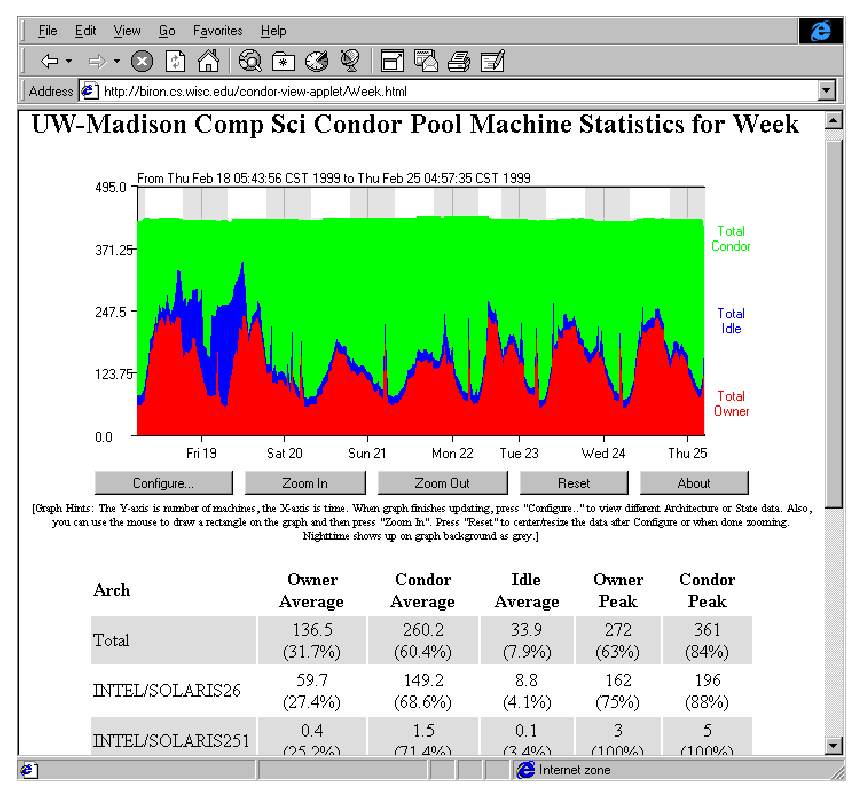
\includegraphics{contrib/view-screenshot.ps}
\caption{\label{fig:view-screenshot}Screen shot of CondorView Client}
\end{figure}

After unpacking and installing the CondorView Client, a script named
\Prog{make\_stats} can be invoked to create HTML pages displaying Condor usage
for the past hour, day, week, or month.  
By using the Unix \Prog{cron} facility to periodically execute
\Prog{make\_stats}, Condor pool usage statistics can be kept up to date
automatically.  
This simple model allows the CondorView Client to be easily installed;
no Web server CGI interface is needed.

%%%%%%%%%%%%%%%%%%%%%%%%%%%%%%%%%%%%%%%%%%%%%%%%%%%%%%%%%%%%%%%%%%%%%%
\subsection{\label{sec:condorview-client-step-by-step}
Step-by-Step Installation of the CondorView Client}
%%%%%%%%%%%%%%%%%%%%%%%%%%%%%%%%%%%%%%%%%%%%%%%%%%%%%%%%%%%%%%%%%%%%%%

\index{installation!CondorView Client}
\index{CondorView!Client installation}
\begin{enumerate}

\item Make certain that the CondorView Server is configured.
Section ~\ref{sec:Contrib-CondorView-Install}
describes configuration of the server.
The server logs information on disk in order to provide a persistent,
historical database of pool statistics.
The CondorView Client makes queries over the network to this
database.
The \Condor{collector} includes this database support.
To activate the persistent database logging, add the following entries to
the configuration file for the \Condor{collector} chosen to act as the ViewServer.
\begin{verbatim}
    POOL_HISTORY_DIR = /full/path/to/directory/to/store/historical/data 
    KEEP_POOL_HISTORY = True 
\end{verbatim}

\item Create a directory where CondorView is to place the HTML files.  
This directory should be one published by a web server, so that HTML
files which exist in this directory can be accessed using a web browser.  
This directory is referred to as the \File{VIEWDIR} directory.

\item Download the \Prog{view\_client} contrib module.
Follow links for contrib modules on the downloads page at
\URL{http://www.cs.wisc.edu/condor/downloads-v2/download.pl}.

\item Unpack or untar this contrib module into the
directory \File{VIEWDIR}.
This creates several files and subdirectories.
Further unpack the jar file within the \File{VIEWDIR} directory with:
\begin{verbatim} 
  jar -xf condorview.jar
\end{verbatim}

\item Edit the \Prog{make\_stats} script.  At the beginning of the file
are six parameters to customize.
The parameters are

        \begin{description}

	\item[\MacroNI{ORGNAME}] A brief name that identifies an
	organization. An example is ``Univ of Wisconsin''.  Do not
	use any slashes in the name or other special regular-expression
	characters. Avoid the characters \Bs \^\  and \$.

	\item[\MacroNI{CONDORADMIN}] The e-mail
	address of the Condor administrator at your site.  
	This e-mail address will appear at the bottom of the web pages.

	\item[\MacroNI{VIEWDIR}] The full path name
	(\emph{not} a relative path) to the \File{VIEWDIR} directory set
	by installation step 2.  
	It is the directory that contains the \Prog{make\_stats} script.

	\item[\MacroNI{STATSDIR}]  The full path name of the
	directory which contains the \Condor{stats} binary.
	The \Condor{stats} program is included in the \Release{bin}
	directory. 
	The value for \MacroNI{STATSDIR} is added to the \MacroNI{PATH}
	parameter by default.  

	\item[\MacroNI{PATH}] A list of subdirectories,
	separated by colons, where the \Prog{make\_stats} script can find
	the \Prog{awk}, \Prog{bc}, \Prog{sed}, \Prog{date}, and \Condor{stats}
	programs.  
	If \Prog{perl} is installed, the path should also
	include the directory where \Prog{perl} is installed.
	The following default works on most systems:
        \begin{verbatim} 
        PATH=/bin:/usr/bin:$STATSDIR:/usr/local/bin
        \end{verbatim}

        \end{description}

\item To create all of the initial HTML files, run
\begin{verbatim}
        ./make_stats setup  
\end{verbatim}
Open the file \File{index.html} to verify that things look good.

\index{CondorView!use of \Prog{crontab} program}
\index{crontab program}

\item Add the \Prog{make\_stats} program to \Prog{cron}.  
Running \Prog{make\_stats} in step 6 created a \File{cronentries} file.
This \File{cronentries} file is ready to be processed by the Unix
\Prog{crontab} command.
The \Prog{crontab} manual page contains details about
the \Prog{crontab} command and the \Prog{cron} daemon.
Look at the
\File{cronentries} file; by default, it will run 
\Prog{make\_stats} \Arg{hour} every 15 minutes, 
\Prog{make\_stats} \Arg{day} once an hour, 
\Prog{make\_stats} \Arg{week} twice per day, and 
\Prog{make\_stats} \Arg{month} once per day.
These are reasonable defaults.  
Add these commands to cron on any
system that can access the \MacroNI{VIEWDIR} and
\MacroNI{STATSDIR} directories,
even on a system that does not have Condor installed.
The commands do not need to run as root user;
in fact, they should probably not run as root.  These commands can run
as any user that has read/write access to the \File{VIEWDIR} directory.
The command
\begin{verbatim} 
  crontab cronentries
\end{verbatim}
can set the crontab file;
note that this command overwrites the current, existing crontab file with the 
entries from the file \File{cronentries}.

\item Point the web browser at the \File{VIEWDIR} directory
to complete the installation.

\end{enumerate}


%%%%%%%%%%%%%%%%%%%%%%%%%%%%%%%%%%%%%%%%%%%%%%%%%%%%%%%%%%%%%%%%%%%%%%
%%%%%%%%%%%%%%%%%%%%%%%%%%%%%%%%%%%%%%%%%%%%%%%%%%%%%%%%%%%%%%%%%%%%%%%%%%%%%%%%
\subsection{\label{sec:Dynamic-Deployment}Dynamic Deployment}
%%%%%%%%%%%%%%%%%%%%%%%%%%%%%%%%%%%%%%%%%%%%%%%%%%%%%%%%%%%%%%%%%%%%%%%%%%%%%%%%
\index{dynamic deployment}
\index{deployment commands}

Dynamic deployment is a mechanism that allows rapid, automated
installation and start up of Condor resources on a given machine.
In this way any machine can be added to a Condor pool.
The dynamic
deployment tool set also provides tools to remove a machine from the
pool, without leaving residual effects on the machine such as leftover
installations, log files, and working directories.

\index{Condor commands!condor\_cold\_start}
Installation and start up is provided by \Condor{cold\_start}.
The \Condor{cold\_start} program determines the operating system and
architecture of the target machine, and transfers the correct
installation package from an ftp, http, or grid ftp site.
After transfer, it
installs Condor and creates a local working
directory for Condor to run in.  As a last step, \Condor{cold\_start}
begins running Condor in a manner which allows for later easy and reliable
shut down.

\index{Condor commands!condor\_cold\_stop}
The program that reliably shuts down and uninstalls a previously
dynamically installed Condor instance is \Condor{cold\_stop}.
\Condor{cold\_stop} begins by safely and reliably shutting off the
running Condor installation.  It ensures that Condor has
completely shut down before continuing, and optionally ensures that
there are no queued jobs at the site.
Next, \Condor{cold\_stop}
removes and optionally archives the Condor working directories,
including the \File{log} directory. 
These archives can be stored to a
mounted file system or to a grid ftp site.
As a last step,
\Condor{cold\_stop} uninstalls the Condor executables and libraries.
The end result is that the machine resources are left unchanged after
a dynamic deployment of Condor leaves.

%%%%%%%%%%%%%%%%%%%%%%%%%%%%%%%%%%%%%%%%%%%%%%%%%%%%%%%%%%%%%%%%%%%%%%%%%%%%%%%%
\subsubsection{Configuration and Usage}
%%%%%%%%%%%%%%%%%%%%%%%%%%%%%%%%%%%%%%%%%%%%%%%%%%%%%%%%%%%%%%%%%%%%%%%%%%%%%%%%

\index{dynamic deployment!configuration}
Dynamic deployment is designed for the expert Condor user
and administrator.
Tool design choices were made for functionality,
not ease-of-use.

Like every installation of Condor, a dynamically deployed installation
relies on a configuration.
To add a target
machine to a previously created Condor pool,
the global configuration file for that pool is a good starting point.
Modifications to that configuration can be made in a separate, 
local configuration file used in the dynamic deployment.
The global configuration file must
be placed on an ftp, http, grid ftp, or file server 
accessible by \Condor{cold\_start}.  The local configuration file
is to be on a file system accessible by the target machine.
There are some specific configuration variables that may be set for
dynamic deployment.  
A list of executables and directories which must be present
for Condor to start on the target machine may be set with
the configuration variables \Macro{DEPLOYMENT\_REQUIRED\_EXECS} and
\Macro{DEPLOYMENT\_REQUIRED\_DIRS}. 
If defined and the comma-separated list of executables or directories are
not present, then \Condor{cold\_start} exits with error.
Note this does not affect what is installed, only
whether start up is successful. 

A list of executables and directories which are recommended to be present
for Condor to start on the target machine may be set with
the configuration variables \Macro{DEPLOYMENT\_RECOMMENDED\_EXECS} and
\Macro{DEPLOYMENT\_RECOMMENDED\_DIRS}. 
If defined and the comma-separated lists of executables or directories are
not present, then \Condor{cold\_start} prints a warning message
and continues.
Here is a portion of the configuration relevant to
a dynamic deployment of a Condor submit node:

\footnotesize
\begin{verbatim}
DEPLOYMENT_REQUIRED_EXECS    = MASTER, SCHEDD, PREEN, STARTER, \
                               STARTER_STANDARD, SHADOW, \
                               SHADOW_STANDARD, GRIDMANAGER, GAHP, CONDOR_GAHP
DEPLOYMENT_REQUIRED_DIRS     = SPOOL, LOG, EXECUTE
DEPLOYMENT_RECOMMENDED_EXECS = CREDD
DEPLOYMENT_RECOMMENDED_DIRS  = LIB, LIBEXEC
\end{verbatim}
\normalsize

Additionally, the user must
specify which Condor services will be started.  This is done through
the \MacroNI{DAEMON\_LIST} configuration variable.  Another excerpt
from a dynamic submit node deployment configuration:

\footnotesize
\begin{verbatim}
DAEMON_LIST  = MASTER, SCHEDD
\end{verbatim}
\normalsize

Finally, the location
of the dynamically installed Condor executables is tricky to set,
since the location is unknown before installation.
Therefore,
the variable \Macro{DEPLOYMENT\_RELEASE\_DIR} is defined in the environment.
It corresponds to the location of the dynamic Condor installation.
If, as is often the case, 
the configuration file specifies the location of Condor executables in
relation to the \MacroNI{RELEASE\_DIR} variable, the configuration can
be made dynamically deployable by setting \MacroNI{RELEASE\_DIR} to
\MacroNI{DEPLOYMENT\_RELEASE\_DIR} as 

\footnotesize
\begin{verbatim}
RELEASE_DIR = $(DEPLOYMENT_RELEASE_DIR)
\end{verbatim}
\normalsize

In addition to setting up the configuration, the user must also
determine where the installation package will reside.
The installation package can be in either tar or 
gzipped tar form, and may
reside on a ftp, http, grid ftp, or file server.  
Create this installation package by tar'ing up the binaries and libraries
needed, and place them on the appropriate server.
The binaries can be tar'ed in a flat structure or within \File{bin} and
\File{sbin}.  Here is a list of files to give an example
structure for a dynamic deployment of the \Condor{schedd} daemon.

\footnotesize
\begin{verbatim}
% tar tfz latest-i686-Linux-2.4.21-37.ELsmp.tar.gz
bin/
bin/condor_config_val
bin/condor_q
sbin/
sbin/condor_preen
sbin/condor_shadow.std
sbin/condor_starter.std
sbin/condor_schedd
sbin/condor_master
sbin/condor_gridmanager
sbin/gahp_server
sbin/condor_starter
sbin/condor_shadow
sbin/condor_c-gahp
sbin/condor_off 
\end{verbatim}
\normalsize

%%%%%%%%%%%%%%%%%%%%%%%%%%%%%%%%%%%%%%%%%%%%%%%%%%%%%%%%%%%%%%%%%%%%%%

%%%%%%%%%%%%%%%%%%%%%%%%%%%%%%%%%%%%%%%%%%%%%%%%%%%%%%%%%%%%%%%%%%%%%%
\section{\label{sec:Configuring-Condor}Configuration}
%%%%%%%%%%%%%%%%%%%%%%%%%%%%%%%%%%%%%%%%%%%%%%%%%%%%%%%%%%%%%%%%%%%%%%

\index{Condor!configuration}
\index{configuration}

This section describes how to configure all parts of the Condor
system.  General information about the configuration
files and their syntax is followed by a description of
settings that affect all
Condor daemons and tools.
The 
settings that control the policy under which Condor will start,
suspend, resume, vacate or kill jobs
are described in 
section~\ref{sec:Configuring-Policy} on Policy Configuration for the
\Condor{startd}. 

%%%%%%%%%%%%%%%%%%%%%%%%%%%%%%%%%%%%%%%%%%%%%%%%%%%%%%%%%%%%%%%%%%%%%%
\subsection{\label{sec:Intro-to-Config-Files}Introduction to
Configuration Files} 
%%%%%%%%%%%%%%%%%%%%%%%%%%%%%%%%%%%%%%%%%%%%%%%%%%%%%%%%%%%%%%%%%%%%%%

The Condor configuration files are used to customize how Condor
operates at a given site.  The basic configuration as shipped with
Condor works well for most sites.

Each Condor program will, as part of its initialization process,
configure itself by calling a library routine which parses the
various configuration files that might be used, including pool-wide,
platform-specific, and machine-specific configuration files.
Environment variables may also contribute to the configuration.

The result of configuration is a list of key/value pairs.
Each key is a configuration variable name,
and each value is a string literal
that may utilize macro substitution (as defined below).
Some configuration variables are evaluated by Condor as ClassAd
expressions; some are not.  Consult the documentation for each specific
case.  Unless otherwise noted, configuration values that are expected
to be numeric or boolean constants may be any valid ClassAd expression
of operators on constants.  Example:

\begin{verbatim}
MINUTE          = 60
HOUR            = (60 * $(MINUTE))
SHUTDOWN_GRACEFUL_TIMEOUT = ($(HOUR)*24)
\end{verbatim}

%%%%%%%%%%%%%%%%%%%%%%%%%%%%%%%%%%%%%%%%%%%%%%%%%%%%%%%%%%%%%%%%%%%%%%
\subsubsection{\label{sec:Ordering-Config-File}Ordered Evaluation to
Set the Configuration} 
%%%%%%%%%%%%%%%%%%%%%%%%%%%%%%%%%%%%%%%%%%%%%%%%%%%%%%%%%%%%%%%%%%%%%%
\index{configuration file!evaluation order}

Multiple files, as well as a program's environment variables
determine the configuration.
The order in which attributes are defined is important, as later
definitions override existing definitions.
The order in which the (multiple) configuration files are parsed 
is designed to ensure the security of the system.
Attributes which must be set a specific way 
must appear in the last file to be parsed.
This prevents both the naive and the malicious Condor user 
from subverting the system through its configuration.
The order in which items are parsed is
\begin{enumerate}
\item global configuration file
\item local configuration file
\item specific environment variables prefixed with \MacroNI{\_CONDOR\_}
\end{enumerate}

The locations for these files are as given in
section~\ref{sec:Config-File-Locations} on
page~\pageref{sec:Config-File-Locations}.

Some Condor tools utilize environment variables to set their
configuration.
These tools search for specifically-named environment variables.
The variables are prefixed by the string \MacroNI{\_CONDOR\_}
or \MacroNI{\_condor\_}.
The tools strip off the prefix, and utilize what remains
as configuration.
As the use of environment variables is the last within
the ordered evaluation, 
the environment variable definition is used.
The security of the system is not compromised,
as only specific variables are considered for definition
in this manner, not any environment variables with
the \MacroNI{\_CONDOR\_} prefix.


%%%%%%%%%%%%%%%%%%%%%%%%%%%%%%%%%%%%%%%%%%%%%%%%%%%%%%%%%%%%%%%%%%%%%%
\subsubsection{\label{sec:Config-File-Macros}Configuration File Macros} 
%%%%%%%%%%%%%%%%%%%%%%%%%%%%%%%%%%%%%%%%%%%%%%%%%%%%%%%%%%%%%%%%%%%%%%

\index{macro!in configuration file}
\index{configuration file!macro definitions}

Macro definitions are of the form:
\begin{verbatim}
<macro_name> = <macro_definition>
\end{verbatim}

The macro name given on the left hand side of the definition is
a case sensitive identifier.
There must be white space between the macro name, the
equals sign (\verb@=@), and the macro definition.
The macro definition is a string literal that may utilize macro substitution.

Macro invocations are of the form: 
\begin{verbatim}
$(macro_name)
\end{verbatim}

Macro definitions may contain references to other macros, even ones
that are not yet defined, as long as they are eventually defined in
the configuration files.
All macro expansion is done after all configuration files have been parsed,
with the exception of macros that reference themselves.

\begin{verbatim}
A = xxx
C = $(A) 
\end{verbatim}
is a legal set of macro definitions, and the resulting value of 
\MacroNI{C} is
\Expr{xxx}.
Note that
\MacroNI{C} is actually bound to 
\MacroUNI{A}, not its value.

As a further example,
\begin{verbatim}
A = xxx
C = $(A)
A = yyy
\end{verbatim}
is also a legal set of macro definitions, and the resulting value of
\MacroNI{C} is \Expr{yyy}.  

A macro may be incrementally defined by invoking itself in its
definition.  For example,
\begin{verbatim}
A = xxx
B = $(A)
A = $(A)yyy
A = $(A)zzz
\end{verbatim}
is a legal set of macro definitions, and the resulting value of 
\MacroNI{A}
is \Expr{xxxyyyzzz}.
Note that invocations of a macro in
its own definition are immediately
expanded.
\MacroUNI{A} is immediately expanded in line 3 of the example.
If it were not, then the definition would be impossible to
evaluate.

Recursively defined macros such as
\begin{verbatim}
A = $(B)
B = $(A)
\end{verbatim}
are \emph{not} allowed.
They create definitions that Condor refuses to parse. 

All entries in a configuration file must have an operator,
which will be an equals sign (\verb@=@).
Identifiers are alphanumerics combined with the underscore character,
optionally with a subsystem name and a period as a prefix.
As a special case,
a line without an operator that begins with a left square bracket
will be ignored.
The following two-line example treats the first line as a comment,
and correctly handles the second line.
\begin{verbatim}
[Condor Settings]
my_classad = [ foo=bar ]
\end{verbatim}

% functionality added to version 6.7.13
To simplify pool administration,
any configuration variable name may be prefixed by
a subsystem 
(see the \MacroUNI{SUBSYSTEM} macro in 
section~\ref{sec:Pre-Defined-Macros}
for the list of subsystems)
and the period (\verb@.@) character.
For configuration variables defined this way,
the value is applied to the specific subsystem.
For example,
the ports that Condor may use can be restricted to a range 
using the \MacroNI{HIGHPORT} and \MacroNI{LOWPORT} configuration
variables.

\begin{verbatim}
  MASTER.LOWPORT   = 20000
  MASTER.HIGHPORT  = 20100
\end{verbatim}

Note that all configuration variables may utilize this syntax,
but nonsense configuration variables may result.
For example, it makes no sense to define
\begin{verbatim}
  NEGOTIATOR.MASTER_UPDATE_INTERVAL = 60
\end{verbatim}
since the \Condor{negotiator} daemon does not use the
\MacroNI{MASTER\_UPDATE\_INTERVAL} variable.

It makes little sense to do so, but Condor will configure
correctly with a definition such as
\begin{verbatim}
  MASTER.MASTER_UPDATE_INTERVAL = 60
\end{verbatim}
The \Condor{master} uses this configuration variable,
and the prefix of \MacroNI{MASTER.} causes this configuration
to be specific to the \Condor{master} daemon.

% the local functionality added in 7.1.4
This syntax has been further expanded to allow for the
specification of a local name on the command line 
using the command line option
\begin{verbatim}
  -local-name <local-name>
\end{verbatim}
This allows multiple instances of a daemon to be run 
by the same \Condor{master} daemon,
each instance with its own local configuration variable.

The ordering used to look up a variable, called \verb@<parameter name>@:

\begin{enumerate}
\item \verb@<subsystem name>.<local name>.<parameter name>@

\item \verb@<local name>.<parameter name>@

\item \verb@<subsystem name>.<parameter name>@

\item \verb@<parameter name>@
\end{enumerate}

If this local name is not specified on the command line, 
numbers 1 and 2 are skipped.
As soon as the first match is found, the search is completed,
and the corresponding value is used.

This example configures a \Condor{master} to run 2 \Condor{schedd}
daemons.  The \Condor{master} daemon needs the configuration:
\begin{verbatim}
  XYZZY           = $(SCHEDD)
  XYZZY_ARGS      = -local-name xyzzy
  DAEMON_LIST     = $(DAEMON_LIST) XYZZY
  DC_DAEMON_LIST  = + XYZZY
  XYZZY_LOG       = $(LOG)/SchedLog.xyzzy
\end{verbatim}

Using this example configuration, the \Condor{master} starts up a
second \Condor{schedd} daemon, 
where this second \Condor{schedd} daemon is passed 
\OptArg{-local-name}{xyzzy}
on the command line.

Continuing the example,
configure the \Condor{schedd} daemon named \Attr{xyzzy}.
This \Condor{schedd} daemon will share all configuration variable
definitions with the other \Condor{schedd} daemon,
except for those specified separately.

\begin{verbatim}
  SCHEDD.XYZZY.SCHEDD_NAME = XYZZY
  SCHEDD.XYZZY.SCHEDD_LOG  = $(XYZZY_LOG)
  SCHEDD.XYZZY.SPOOL       = $(SPOOL).XYZZY
\end{verbatim}

Note that the example \MacroNI{SCHEDD\_NAME} and \MacroNI{SPOOL} are
specific to the \Condor{schedd} daemon, as opposed to a different daemon
such as the \Condor{startd}.
Other Condor daemons using this feature will
have different requirements for which parameters need to be
specified individually.  This example works for the \Condor{schedd},
and more local configuration can, and likely would be specified.

Also note that each daemon's log file must be specified individually,
and in two places: one specification is for use by the \Condor{master},
and the other is for use by the daemon itself.
In the example,
the \Attr{XYZZY} \Condor{schedd} configuration variable
\MacroNI{SCHEDD.XYZZY.SCHEDD\_LOG} definition references the
\Condor{master} daemon's \MacroNI{XYZZY\_LOG}.


%%%%%%%%%%%%%%%%%%%%%%%%%%%%%%%%%%%%%%%%%%%%%%%%%%%%%%%%%%%%%%%%%%%%%%
\subsubsection{\label{sec:Other-Syntax}Comments and Line Continuations}
%%%%%%%%%%%%%%%%%%%%%%%%%%%%%%%%%%%%%%%%%%%%%%%%%%%%%%%%%%%%%%%%%%%%%%

A Condor configuration file may contain comments and
line continuations.
A comment is any line beginning with a pound character (\verb@#@).
A continuation is any entry that continues across multiples lines.
Line continuation is accomplished by placing the backslash
character (\Bs) at the end of any line to be continued onto another.
Valid examples of line continuation are
\begin{verbatim}
  START = (KeyboardIdle > 15 * $(MINUTE)) && \
  ((LoadAvg - CondorLoadAvg) <= 0.3)
\end{verbatim}
and
\begin{verbatim}
  ADMIN_MACHINES = condor.cs.wisc.edu, raven.cs.wisc.edu, \
  stork.cs.wisc.edu, ostrich.cs.wisc.edu, \
  bigbird.cs.wisc.edu
  HOSTALLOW_ADMINISTRATOR = $(ADMIN_MACHINES)
\end{verbatim}

Note that a line continuation character may currently be used within
a comment, so the following example does \emph{not} set the
configuration variable \MacroNI{FOO}:
\begin{verbatim}
  # This comment includes the following line, so FOO is NOT set \
  FOO = BAR
\end{verbatim}
It is a poor idea to use this functionality.

%%%%%%%%%%%%%%%%%%%%%%%%%%%%%%%%%%%%%%%%%%%%%%%%%%%%%%%%%%%%%%%%%%%%%%
\subsubsection{\label{sec:Program-Defined-Macros}Executing a Program to Produce Configuration Macros}
%%%%%%%%%%%%%%%%%%%%%%%%%%%%%%%%%%%%%%%%%%%%%%%%%%%%%%%%%%%%%%%%%%%%%%

Instead of reading from a file,
Condor may run a program to obtain configuration macros.
The vertical bar character (\Bar) as the last character defining
a file name provides the syntax necessary to tell 
Condor to run a program.
This syntax may only be used in the definition of
the \Env{CONDOR\_CONFIG} environment variable,
or the \Macro{LOCAL\_CONFIG\_FILE} configuration variable.

The command line for the program 
is formed by the characters preceding the vertical bar character.
The standard output of the program is parsed as a configuration 
file would be.

An example:
\begin{verbatim}
LOCAL_CONFIG_FILE = /bin/make_the_config|
\end{verbatim}

Program \Prog{/bin/make\_the\_config} is executed, and its output
is the set of configuration macros.

Note that either a program is executed to generate the
configuration macros or the configuration is read from 
one or more files.
The syntax uses space characters to separate command line elements,
if an executed program produces the configuration macros.
Space characters would otherwise separate the list of files.
This syntax does not permit distinguishing one from the other,
so only one may be specified.

%%%%%%%%%%%%%%%%%%%%%%%%%%%%%%%%%%%%%%%%%%%%%%%%%%%%%%%%%%%%%%%%%%%%%%
\subsubsection{\label{sec:Macros-Requiring-Restart}Macros That Will Require a Restart When Changed}
%%%%%%%%%%%%%%%%%%%%%%%%%%%%%%%%%%%%%%%%%%%%%%%%%%%%%%%%%%%%%%%%%%%%%%
\index{configuration change requiring a restart of Condor}
When any of the following listed configuration variables are changed,
Condor must be restarted.
Reconfiguration using \Condor{reconfig} will not be enough.

\begin{itemize}
  \item \verb@BIND_ALL_INTERFACES@
  \item \verb@FetchWorkDelay@
  \item \verb@MAX_NUM_CPUS@
  \item \verb@MAX_TRACKING_GID@
  \item \verb@MIN_TRACKING_GID@
  \item \verb@NETWORK_INTERFACE@
  \item \verb@NUM_CPUS@
  \item \verb@PREEMPTION_REQUIREMENTS_STABLE@
  \item \verb@PRIVSEP_ENABLED@
  \item \verb@PROCD_ADDRESS@
\end{itemize}

%%%%%%%%%%%%%%%%%%%%%%%%%%%%%%%%%%%%%%%%%%%%%%%%%%%%%%%%%%%%%%%%%%%%%%
\subsubsection{\label{sec:Pre-Defined-Macros}Pre-Defined Macros}
%%%%%%%%%%%%%%%%%%%%%%%%%%%%%%%%%%%%%%%%%%%%%%%%%%%%%%%%%%%%%%%%%%%%%%

\index{configuration!pre-defined macros}
\index{configuration file!pre-defined macros}
Condor provides pre-defined macros that help configure Condor.
Pre-defined macros are listed as \MacroUNI{macro\_name}.

This first set are entries whose values are determined at
run time and cannot be overwritten.  These are inserted automatically by
the library routine which parses the configuration files.
This implies that a change to the underlying value of any of these
variables will require a full restart of Condor in order to use
the changed value.
\begin{description}
  
\label{param:FullHostname}
\item[\MacroU{FULL\_HOSTNAME}]
  The fully qualified host name of the local machine, 
  which is host name plus domain name.
  
\label{param:Hostname}
\item[\MacroU{HOSTNAME}]
  The host name of the local machine, \emph{without} a domain name.
  
\label{param:IpAddress}
\item[\MacroU{IP\_ADDRESS}]
  The ASCII string version of the local machine's IP address.

\label{param:Tilde}
\item[\MacroU{TILDE}]
  The full path to the
  home directory of the Unix user \Login{condor}, if such a user exists on the
  local machine.

  \label{sec:Condor-Subsystem-Names}
  \index{configuration file!subsystem names}
\label{param:Subsystem}
\item[\MacroU{SUBSYSTEM}]
  The subsystem
  name of the daemon or tool that is evaluating the macro.
  This is a unique string which identifies a given daemon within the
  Condor system.  The possible subsystem names are:

  \index{subsystem names}
  \index{macro!subsystem names}
  \begin{itemize}
  \label{list:subsystem names}
  \item \verb@C_GAHP@
  \item \verb@CKPT_SERVER@
  \item \verb@COLLECTOR@
  \item \verb@DBMSD@
  \item \verb@DEFRAG@
  \item \verb@EC2_GAHP@
  \item \verb@GRIDMANAGER@
  \item \verb@HAD@
  \item \verb@HDFS@
  \item \verb@JOB_ROUTER@
  \item \verb@KBDD@ 
  \item \verb@LEASEMANAGER@
  \item \verb@MASTER@
  \item \verb@NEGOTIATOR@
  \item \verb@QUILL@
  \item \verb@REPLICATION@
  \item \verb@ROOSTER@
  \item \verb@SCHEDD@
  \item \verb@SHADOW@
  \item \verb@STARTD@
  \item \verb@STARTER@
  %\item \verb@STORK@
  \item \verb@SUBMIT@
  \item \verb@TOOL@
  \item \verb@TRANSFERER@
  \end{itemize}

\end{description}

This second set of macros are entries whose default values are
determined automatically at run time but which can be overwritten.  
\index{configuration file!macros}
\begin{description}

\label{param:Arch}
\item[\MacroU{ARCH}]
  Defines the string
  used to identify the architecture of the local machine to Condor.
  The \Condor{startd} will advertise itself with this attribute so
  that users can submit binaries compiled for a given platform and
  force them to run on the correct machines.  \Condor{submit} will
  append a requirement to the job ClassAd that it must
  run on the same \MacroNI{ARCH} and \MacroNI{OPSYS} of the machine where
  it was submitted, unless the user specifies \MacroNI{ARCH} and/or
  \MacroNI{OPSYS} explicitly in their submit file.  See the
  the \Condor{submit} manual page
  on page~\pageref{man-condor-submit} for details.

\label{param:OpSys}
\item[\MacroU{OPSYS}]
  Defines the string used to identify the operating system
  of the local machine to Condor.
  If it is not defined in the configuration file, Condor will
  automatically insert the operating system of this machine as
  determined by \Prog{uname}.

\label{param:OpSysVer}
\item[\MacroU{OPSYS\_VER}]
  Defines the integer used to identify the operating system version number.

\label{param:OpSysAndVer}
\item[\MacroU{OPSYS\_AND\_VER}]
  Defines the string used prior to Condor version 7.7.2 as \MacroUNI{OPSYS}.

\label{param:UnameArch}
\item[\MacroU{UNAME\_ARCH}]
  The architecture as reported by \Prog{uname}(2)'s \Code{machine} field.
  Always the same as \MacroNI{ARCH} on Windows.

\label{param:UnameOpsys}
\item[\MacroU{UNAME\_OPSYS}]
  The operating system as reported by \Prog{uname}(2)'s \Code{sysname} field.
  Always the same as \MacroNI{OPSYS} on Windows.

\label{param:DetectedMemory}
\item[\MacroU{DETECTED\_MEMORY}]
  The amount of detected physical memory (RAM) in Mbytes.

\label{param:DetectedCores}
\item[\MacroU{DETECTED\_CORES}]
  The number of detected CPU cores.  
  This includes hyper threaded cores, if there are any.

\label{param:Pid}
\item[\MacroU{PID}]
  The process ID for the daemon or tool.

\label{param:Ppid}
\item[\MacroU{PPID}]
  The process ID of the parent process for the daemon or tool.

\label{param:Username}
\item[\MacroU{USERNAME}]
  The user name of the UID of the daemon or tool.
  For daemons started as root, but running under another UID
  (typically the user \Login{condor}), this will be the other UID.

\label{param:FilesystemDomain}
\item[\MacroU{FILESYSTEM\_DOMAIN}]
  Defaults to the fully
  qualified host name of the machine it is evaluated on.  See
  section~\ref{sec:Shared-Filesystem-Config-File-Entries}, Shared
  File System Configuration File Entries for the full description of
  its use and under what conditions it could be desirable to change it.

\label{param:UIDDomain}
\item[\MacroU{UID\_DOMAIN}]
  Defaults to the fully
  qualified host name of the machine it is evaluated on.  See
  section~\ref{sec:Shared-Filesystem-Config-File-Entries} 
  for the full description of this configuration variable.

\end{description}

Since \MacroUNI{ARCH} and \MacroUNI{OPSYS} will automatically be set to the
correct values, we recommend that you do not overwrite them.


%%%%%%%%%%%%%%%%%%%%%%%%%%%%%%%%%%%%%%%%%%%%%%%%%%%%%%%%%%%%%%%%%%%%%%
\subsection{\label{sec:Config-File-Special}Special Macros}
%%%%%%%%%%%%%%%%%%%%%%%%%%%%%%%%%%%%%%%%%%%%%%%%%%%%%%%%%%%%%%%%%%%%%%

\index{configuration file!\$ENV definition}
\index{\$ENV!in configuration file}
References to the Condor process's environment are allowed in the
configuration files.
Environment references use the \Macro{ENV} macro and are of the form:
\begin{verbatim}
  $ENV(environment_variable_name)
\end{verbatim}
For example, 
\begin{verbatim}
  A = $ENV(HOME)
\end{verbatim}
binds \MacroNI{A} to the value of the \Env{HOME} environment variable.
Environment references are not currently used in standard Condor
configurations.
However, they can sometimes be useful in custom configurations.

\index{\$RANDOM\_CHOICE()!in configuration}
This same syntax is used in the \Macro{RANDOM\_CHOICE()} macro to
allow a random choice of a parameter
within a configuration file.
These references are of the form:
\begin{verbatim}
  $RANDOM_CHOICE(list of parameters)
\end{verbatim}
This allows a random choice within the parameter list to be made
at configuration time.  Of the list of parameters, one is
chosen when encountered during configuration.  For example,
if one of the integers 0-8 (inclusive) should be randomly
chosen, the macro usage is
\begin{verbatim}
  $RANDOM_CHOICE(0,1,2,3,4,5,6,7,8)
\end{verbatim}

\index{\$RANDOM\_INTEGER()!in configuration}
The \Macro{RANDOM\_INTEGER()} macro is similar to the \MacroNI{RANDOM\_CHOICE()}
macro, and is used to select a random integer within a configuration file.
References are of the form:
\begin{verbatim}
  $RANDOM_INTEGER(min, max [, step])
\end{verbatim}
A random integer within the range \verb@min@ and \verb@max@, inclusive,
is selected at configuration time.
The optional \verb@step@ parameter
controls the stride within the range, and it defaults to the value 1.
For example, to randomly chose an even integer in the range 0-8 (inclusive),
the macro usage is
\begin{verbatim}
  $RANDOM_INTEGER(0, 8, 2)
\end{verbatim}

See section~\ref{sec:randomintegerusage} on
page~\pageref{sec:randomintegerusage}
for an actual use of this specialized macro.
%%%%%%%%%%%%%%%%%%%%%%%%%%%%%%%%%%%%%%%%%%%%%%%%%%%%%%%%%%%%%%%%%%%%%%
\subsection{\label{sec:Condor-wide-Config-File-Entries}Condor-wide Configuration File Entries} 
%%%%%%%%%%%%%%%%%%%%%%%%%%%%%%%%%%%%%%%%%%%%%%%%%%%%%%%%%%%%%%%%%%%%%%

\index{configuration!Condor-wide configuration variables}

This section describes settings which affect all parts of the Condor
system. 
Other system-wide settings can be found in
section~\ref{sec:Network-Related-Config-File-Entries} on
``Network-Related Configuration File Entries'', and
section~\ref{sec:Shared-Filesystem-Config-File-Entries} on ``Shared
File System Configuration File Entries''. 

\begin{description}
  
\label{param:CondorHost}
\item[\Macro{CONDOR\_HOST}]
  This macro is used to define the
  \MacroUNI{COLLECTOR\_HOST} macro.  Normally the \Condor{collector}
  and \Condor{negotiator} would run on the same machine.  If for some
  reason they were not run on the same machine,
  \MacroUNI{CONDOR\_HOST} would not be needed.  Some
  of the host-based security macros use \MacroUNI{CONDOR\_HOST} by
  default.  See section~\ref{sec:Host-Security}, on Setting up
  IP/host-based security in Condor for details.
  
\label{param:CollectorHost}
\item[\Macro{COLLECTOR\_HOST}]
  The host name of the machine where the \Condor{collector} is running for
  your pool.  Normally, it is defined relative to
  the \MacroUNI{CONDOR\_HOST}
  macro.  There is no default value for this macro;
  \MacroNI{COLLECTOR\_HOST} must be defined for the pool to work
  properly.

  In addition to defining the host name, this setting can optionally be
  used to specify the network port of the \Condor{collector}.
  The port is separated from the host name by a colon ('\verb@:@').
  For example,
  \begin{verbatim}
    COLLECTOR_HOST = $(CONDOR_HOST):1234
  \end{verbatim}
  If no port is specified, the default port of 9618 is used.
  Using the default port is recommended for most sites.
  It is only changed if there is a conflict with another
  service listening on the same network port.
  For more information about specifying a non-standard port for the
  \Condor{collector} daemon,
  see section~\ref{sec:Ports-NonStandard} on
  page~\pageref{sec:Ports-NonStandard}.


\label{param:NegotiatorHost} 
\item[\Macro{NEGOTIATOR\_HOST}]
  This configuration variable is no longer used.
  It previously defined the host name of the machine where 
  the \Condor{negotiator} is running.
  At present, the port where the \Condor{negotiator} is listening 
  is dynamically allocated. 

  % commented out by Karen in 2008, as this 6.7ism is too old
  %For pools running 6.7.3 and older versions: The
  %host name of the machine where the \Condor{negotiator} is running for
  %the pool.
  %Normally, it is defined relative to the \MacroUNI{CONDOR\_HOST}
  %macro.  There is no default value for this macro;
  %\MacroNI{NEGOTIATOR\_HOST} must be defined for the pool to work
  %properly.
  %This variable may also be used to optionally define a network port for
  %the \Condor{negotiator} daemon, as explained for the
  %\MacroNI{COLLECTOR\_HOST} variable.

\label{param:CondorViewHost}
\item[\Macro{CONDOR\_VIEW\_HOST}]
  A list of CondorView servers, separated by commas and/or spaces.
  Each CondorView server is denoted by the host name of the machine
  it is running on, optionally appended by a colon and the port number.
  This service is optional, and requires additional configuration 
  to enable it.  There is no default value for
  \MacroNI{CONDOR\_VIEW\_HOST}.  If \MacroNI{CONDOR\_VIEW\_HOST} is not
  defined, no CondorView server is used.
  See section~\ref{sec:Contrib-CondorView-Install} on
  page~\pageref{sec:Contrib-CondorView-Install} for more details.

\label{param:ScheddHost}
\item[\Macro{SCHEDD\_HOST}]
  The host name of the machine where the \Condor{schedd} is running for
  your pool.  This is the host that queues submitted jobs.
  If the host specifies \Macro{SCHEDD\_NAME} or \Macro{MASTER\_NAME}, that
  name must be included in the form name\verb$@$hostname.
  In most condor installations, there is a \Condor{schedd} running on
  each host from which jobs are submitted.  The default value of
  \Macro{SCHEDD\_HOST} is the current host with the optional name included.  For most pools, this
  macro is not defined, nor does it need to be defined..

\label{param:ReleaseDir}
\item[\Macro{RELEASE\_DIR}]
  The full path to
  the Condor release directory, which holds the \File{bin},
  \File{etc}, \File{lib}, and \File{sbin} directories.  Other macros
  are defined relative to this one.  There is no default value for
  \Macro{RELEASE\_DIR}.

\label{param:Bin}
\item[\Macro{BIN}]
  This directory points to the
  Condor directory where user-level programs are installed.  It is
  usually defined relative to the \MacroUNI{RELEASE\_DIR} macro.
  There is no default value for \Macro{BIN}.
  
\label{param:Lib}
\item[\Macro{LIB}]
  This directory points to the
  Condor directory where libraries used to link jobs for Condor's
  standard universe are stored.  The \Condor{compile} program uses
  this macro to find these libraries, so it must be defined for
  \Condor{compile} to function.  \MacroUNI{LIB} is usually defined
  relative to the \MacroUNI{RELEASE\_DIR} macro, and has no default
  value.

\label{param:LibExec}
\item[\Macro{LIBEXEC}]
  This directory points
  to the Condor directory where support commands that Condor
  needs will be placed.
  Do not add this directory to a user or system-wide path.

\label{param:Include}
\item[\Macro{INCLUDE}]
  This directory points to the Condor directory where header files reside.
  \MacroUNI{INCLUDE} would usually be defined relative to
  the \MacroUNI{RELEASE\_DIR} configuration macro.
  There is no default value, but
  if defined, it can make inclusion of necessary header files
  for compilation of programs (such as those programs
  that use \File{libcondorapi.a})
  easier through the use of \Condor{config\_val}.

\label{param:Sbin}
\item[\Macro{SBIN}]
  This directory points to the
  Condor directory where Condor's system binaries (such as the
  binaries for the Condor daemons) and administrative tools are
  installed.  Whatever directory \MacroU{SBIN} points to ought
  to be in the \Env{PATH} of users acting as Condor
  administrators.  \Macro{SBIN} has no default value.

\label{param:LocalDir}
\item[\Macro{LOCAL\_DIR}]
  The location of the
  local Condor directory on each machine in your pool.  One common
  option is to use the condor user's home directory which may be
  specified with \MacroUNI{TILDE}.  There is no default value for
  \Macro{LOCAL\_DIR}.  For example:
  \begin{verbatim}
    LOCAL_DIR = $(tilde)
  \end{verbatim}
  
  On machines with a shared file system, where either the
  \MacroUNI{TILDE} directory or another directory you want to use is
  shared among all machines in your pool, you might use the
  \MacroUNI{HOSTNAME} macro and have a directory with many
  subdirectories, one for each machine in your pool, each named by
  host names.  For example:
  \begin{verbatim}
    LOCAL_DIR = $(tilde)/hosts/$(hostname)      
  \end{verbatim}
  or:
  \begin{verbatim}
    LOCAL_DIR = $(release_dir)/hosts/$(hostname)
  \end{verbatim}
  
\label{param:Log}
\item[\Macro{LOG}]
  Used to specify the
  directory where each Condor daemon writes its log files.  The names
  of the log files themselves are defined with other macros, which use
  the \MacroUNI{LOG} macro by default.  The log directory also acts as
  the current working directory of the Condor daemons as the run, so
  if one of them should produce a core file for any reason, it would
  be placed in the directory defined by this macro.  \MacroNI{LOG} is
  required to be defined.  Normally, \MacroUNI{LOG} is defined in
  terms of \MacroUNI{LOCAL\_DIR}.

\label{param:Run}
\item[\Macro{RUN}]
  A path and directory name to be used by the Condor init script to 
  specify the directory where the \Condor{master} should write its process ID
  (PID) file. 
  The default if not defined is \MacroUNI{LOG}.
  
\label{param:Spool}
\item[\Macro{SPOOL}]
  The spool directory is where
  certain files used by the \Condor{schedd} are stored, such as the
  job queue file and the initial executables of any jobs that have
  been submitted.  In addition, for systems not using a checkpoint
  server, all the checkpoint files from jobs that have been submitted
  from a given machine will be store in that machine's spool
  directory.  Therefore, you will want to ensure that the spool
  directory is located on a partition with enough disk space.  If a
  given machine is only set up to execute Condor jobs and not submit
  them, it would not need a spool directory (or this macro defined).
  There is no default value for \Macro{SPOOL}, and the \Condor{schedd}
  will not function without it \Macro{SPOOL} defined.  Normally,
  \MacroUNI{SPOOL} is defined in terms of \MacroUNI{LOCAL\_DIR}.
  
\label{param:Execute}
\item[\Macro{EXECUTE}]
  This directory acts as
  a place to create the scratch directory of any Condor job that is executing
  on
  the local machine.  The scratch directory is the destination of
  any input files that were specified for transfer.  It also serves
  as the job's working directory if the job is using file transfer
  mode and no other working directory was specified.
  If a given machine is set up to only submit
  jobs and not execute them, it would not need an execute directory,
  and this macro need not be defined.  There is no default value for
  \MacroNI{EXECUTE}, and the \Condor{startd} will not function if
  \MacroNI{EXECUTE} is undefined.  Normally, \MacroUNI{EXECUTE} is
  defined in terms of \MacroUNI{LOCAL\_DIR}.  To customize the execute
  directory independently for each batch slot, use \MacroNI{SLOT<N>\_EXECUTE}.

\label{param:SlotNExecute}
\item[\Macro{SLOT<N>\_EXECUTE}]
  Specifies an
  execute directory for use by a specific batch slot.
  \MacroNI{<N>} represents the number of the batch slot, such as 1, 2, 3, etc.
  This execute directory serves the same purpose as \Macro{EXECUTE}, but it
  allows the configuration of the directory independently for each batch
  slot.  Having slots each using a different partition would be
  useful, for example, in preventing one job from filling up the same
  disk that other jobs are trying to write to.  If this parameter is
  undefined for a given batch slot, it will use \MacroNI{EXECUTE} as
  the default.  Note that each slot will advertise \AdAttr{TotalDisk}
  and \AdAttr{Disk} for the partition containing its execute
  directory.

\label{param:LocalConfigFile}
\item[\Macro{LOCAL\_CONFIG\_FILE}]
  Identifies the
  location of the local, machine-specific configuration
  file for each machine
  in the pool.  The two most common choices would be putting this
  file in the \MacroUNI{LOCAL\_DIR}, or putting all
  local configuration files for the pool in a shared directory, each one
  named by host name.  For example,
  \begin{verbatim}
    LOCAL_CONFIG_FILE = $(LOCAL_DIR)/condor_config.local
  \end{verbatim}
  or,
  \begin{verbatim}
    LOCAL_CONFIG_FILE = $(release_dir)/etc/$(hostname).local
  \end{verbatim}
  or, not using the release directory
  \begin{verbatim}
    LOCAL_CONFIG_FILE = /full/path/to/configs/$(hostname).local
  \end{verbatim}
  
  The value of \MacroNI{LOCAL\_CONFIG\_FILE} is treated as a list of files,
  not a
  single file.  The items in the list are delimited by either commas
  or space characters.
  This allows the specification of multiple files as
  the local configuration file, each one processed in the
  order given (with parameters set in later files overriding values
  from previous files).  This allows the use of one global
  configuration file for multiple platforms in the pool, defines a
  platform-specific configuration file for each platform, and uses a
  local configuration file for each machine. 
  If the list of files is changed in one of the later read files, the new list
  replaces the old list, but any files that have already been processed
  remain processed, and are removed from the new list if they are present
  to prevent cycles.
  See section~\ref{sec:Program-Defined-Macros} on 
  page~\pageref{sec:Program-Defined-Macros} for directions on
  using a program to generate the configuration macros that would
  otherwise reside in one or more files as described here.
  If \MacroNI{LOCAL\_CONFIG\_FILE} is not defined, no local configuration
  files are processed.  For more information on this, see
  section~\ref{sec:Multiple-Platforms} about Configuring Condor for
  Multiple Platforms on page~\pageref{sec:Multiple-Platforms}.

  If all files in a directory are local configuration files to be processed,
  then consider using \MacroNI{LOCAL\_CONFIG\_DIR}, defined at
  section~\ref{param:LocalConfigDir}.

\label{param:RequireLocalConfigFile}
\item[\Macro{REQUIRE\_LOCAL\_CONFIG\_FILE}]
  A boolean value that defaults to \Expr{True}.
  When \Expr{True}, Condor exits with an error,
  if any file listed in \MacroNI{LOCAL\_CONFIG\_FILE} cannot be read.
  A value of \Expr{False} allows local configuration files to be missing.
  This is most useful for sites that have 
  both large numbers of machines in the pool and a local configuration file
  that uses the \MacroUNI{HOSTNAME} macro in its definition.
  Instead of having an empty file for every host
  in the pool, files can simply be omitted.

\label{param:LocalConfigDir} 
\item[\Macro{LOCAL\_CONFIG\_DIR}]
  A directory may be used as a container for local configuration files. 
  The files found in the directory are sorted into lexicographical order 
  by file name, and 
  then each file is treated as though it was listed in 
  \MacroNI{LOCAL\_CONFIG\_FILE}. 
  \MacroNI{LOCAL\_CONFIG\_DIR} is processed before any files listed in 
  \MacroNI{LOCAL\_CONFIG\_FILE}, and is checked again after processing
  the \MacroNI{LOCAL\_CONFIG\_FILE} list. 
  It is a list of directories, and each directory is processed in the order
  it appears in the list. 
  The process is not recursive, so any directories found inside the directory
  being processed are ignored. 
  See also \MacroNI{LOCAL\_CONFIG\_DIR\_EXCLUDE\_REGEXP}.

\label{param:LocalConfigDirExcludeRegexp}
\item[\Macro{LOCAL\_CONFIG\_DIR\_EXCLUDE\_REGEXP}]
  A regular expression that specifies file names to be ignored when
  looking for configuration files within the directories specified via
  \MacroNI{LOCAL\_CONFIG\_DIR}.  The default expression ignores files
  with names beginning with a `.' or a `\verb|#|', as well as files with names
  ending in `\~{}'.  This avoids accidents that can be caused by
  treating temporary files created by text editors as configuration
  files.

\label{param:CondorIds}
\item[\Macro{CONDOR\_IDS}]
  The User ID (UID) and Group ID (GID) pair that the Condor daemons
  should run as, if the daemons are spawned as root.
  This value can also be specified in the \Env{CONDOR\_IDS}
  environment variable.
  If the Condor daemons are not started as root, then neither this
  \MacroNI{CONDOR\_IDS} configuration macro nor the \Env{CONDOR\_IDS}
  environment variable are used.
  The value is given by two integers, separated by a period.  For
  example, \verb@CONDOR_IDS = 1234.1234@.
  If this pair is not specified in either the configuration file or in the
  environment, and the Condor daemons are spawned as root,
  then Condor will
  search for a \verb@condor@ user on the system, and run as that user's
  UID and GID.
  See section~\ref{sec:uids} on UIDs in Condor for more details.

\label{param:CondorAdmin}
\item[\Macro{CONDOR\_ADMIN}]
  The email address that Condor will send mail to if something goes wrong in
  the pool.  For example, if a daemon crashes, the \Condor{master}
  can send an \Term{obituary} to this address with the last few lines
  of that daemon's log file and a brief message that describes what
  signal or exit status that daemon exited with.  There is no default
  value for \MacroNI{CONDOR\_ADMIN}.

\label{param:SubsysAdminEmail}
\item[\MacroB{<SUBSYS>\_ADMIN\_EMAIL}]
\index{SUBSYS\_ADMIN\_EMAIL macro@\texttt{<SUBSYS>\_ADMIN\_EMAIL} macro}
  The email address that Condor will send mail to if something goes wrong
  with the named \MacroNI{<SUBSYS>}.  Identical to \MacroNI{CONDOR\_ADMIN},
  but done on a per subsystem basis. There is no default value.
  
\label{param:CondorSupportEmail}
\item[\Macro{CONDOR\_SUPPORT\_EMAIL}]
  The email address to be included at the bottom of all email Condor
  sends out under the label ``Email address of the local Condor
  administrator:''.  
  This is the address where Condor users at your site should send
  their questions about Condor and get technical support.
  If this setting is not defined, Condor will use the address
  specified in \MacroNI{CONDOR\_ADMIN} (described above).

\label{param:EmailSignature}
\item[\Macro{EMAIL\_SIGNATURE}]
  Every e-mail sent by Condor includes a short signature line appended
  to the body.  By default, this signature includes the URL to the
  global Condor project website.  
  When set, this variable defines an alternative signature line to be
  used instead of the default. 
  Note that the value can only be one line in length.
  This variable could be used to direct users
  to look at local web site with information specific to the installation
  of Condor.

\label{param:Mail}
\item[\Macro{MAIL}]
  The full path to a mail
  sending program that uses \Opt{-s} to specify a subject for the
  message.  On all platforms, the default shipped with Condor should
  work.  Only if you installed things in a non-standard location on
  your system would you need to change this setting.  There is no
  default value for \MacroNI{MAIL}, and the \Condor{schedd} will not
  function unless \MacroNI{MAIL} is defined.

\label{param:MailFrom}
\item[\Macro{MAIL\_FROM}]
  The e-mail address that notification e-mails appear to come from.
  Contents is that of the \Expr{From} header.
  There is no default value; if undefined, the \Expr{From} header may
  be nonsensical.

\label{param:SMTPServer}
\item[\Macro{SMTP\_SERVER}]
  For Windows platforms only, the host name of the server through which
  to route notification e-mail.
  There is no default value; if undefined and the debug level is
  at  \Expr{FULLDEBUG}, an error message will be generated.

\label{param:ReservedSwap}
\item[\Macro{RESERVED\_SWAP}]
  The amount of swap space in Mbytes to reserve for this machine.
  Condor will not start up more \Condor{shadow} processes if the
  amount of free swap space on this machine falls below this level.
  The default value is 0, which disables this check.
  It is anticipated that this configuration variable will no longer
  be used in the near future.
  If \MacroNI{RESERVED\_SWAP} is \emph{not} set to 0,
  the value of \Macro{SHADOW\_SIZE\_ESTIMATE} is used.

\label{param:ReservedDisk}
\item[\Macro{RESERVED\_DISK}]
  Determines how much disk space you want to reserve for your own machine.
  When Condor is reporting the amount of free disk space in a given
  partition on your machine, it will always subtract this amount.  An
  example is the \Condor{startd}, which advertises the amount of free
  space in the \MacroUNI{EXECUTE} directory.  The default value of
  \Macro{RESERVED\_DISK} is zero.
  
\label{param:Lock}
\item[\Macro{LOCK}]
  Condor needs to create
  lock files to synchronize access to various log files.  Because of
  problems with network file systems and file locking over
  the years, we \emph{highly} recommend that you put these lock
  files on a local partition on each machine.  If you do not have your
  \MacroUNI{LOCAL\_DIR} on a local partition, be sure to change this
  entry.

  Whatever user or group Condor is running as needs to have
  write access to this directory.  If you are not running as root, this
  is whatever user you started up the \Condor{master} as.  If you are
  running as root, and there is a condor account, it is most
  likely condor.
  Otherwise, it is whatever you set in the \Env{CONDOR\_IDS}
  \index{environment variables!CONDOR\_IDS@\texttt{CONDOR\_IDS}}
  \index{CONDOR\_IDS@\texttt{CONDOR\_IDS}!environment variable}
  environment variable, or whatever you define in the
  \MacroNI{CONDOR\_IDS} setting in the Condor config files.
  See section~\ref{sec:uids} on UIDs in Condor for details.

  If no value for \MacroNI{LOCK} is provided, the value of \MacroNI{LOG}
  is used.


\label{param:History}
\item[\Macro{HISTORY}]
  Defines the
  location of the Condor history file, which stores information about
  all Condor jobs that have completed on a given machine.  This macro
  is used by both the \Condor{schedd} which appends the information
  and \Condor{history}, the user-level program used to view
  the history file.
  This configuration macro is given the default value of
  \File{\$(SPOOL)/history} in the default configuration.
  If not defined,
  no history file is kept.
  % PKK
  % Described in default config file: YES
  % Defined in the default config file: YES 
  % Default definition in config file: $(SPOOL)/history
  % Result if not defined or RHS is empty: no history file is kept.

\label{param:EnableHistoryRotation} 
\item[\Macro{ENABLE\_HISTORY\_ROTATION}]
  If this is defined to be true, then the
  history file will be rotated. If it is false, then it will not be
  rotated, and it will grow indefinitely, to the limits allowed by the
  operating system. If this is not defined, it is assumed to be
  true. The rotated files will be stored in the same directory as the
  history file. 

\label{param:MaxHistoryLog}
\item[\Macro{MAX\_HISTORY\_LOG}]
  Defines the maximum size for the history file, in bytes. It defaults
  to 20MB. This parameter is only used if history file rotation is
  enabled. 

\label{param:MaxHistoryRotations}
\item[\Macro{MAX\_HISTORY\_ROTATIONS}]
  When history file rotation is turned on, this controls how many
  backup files there are. It default to 2, which means that there may
  be up to three history files (two backups, plus the history file
  that is being currently written to). When the history file is
  rotated, and this rotation would cause the number of backups to be
  too large, the oldest file is removed. 

\label{param:MaxJobQueueLogRotations}
\item[\Macro{MAX\_JOB\_QUEUE\_LOG\_ROTATIONS}]
  The schedd periodically rotates the job queue database file in order
  to save disk space.  This option controls how many rotated files are
  saved.  It defaults to 1, which means there may be up to two history
  files (the previous one, which was rotated out of use, and the current one
  that is being written to).  When the job queue file is rotated,
  and this rotation would cause the number of backups to be larger
  the the maximum specified, the oldest file is removed.

\label{param:ClassadLogStrictParsing}
\item[\Macro{CLASSAD\_LOG\_STRICT\_PARSING}]
  A boolean value that defaults to \Expr{True}. 
  When \Expr{True}, ClassAd log files will be read using 
  a strict syntax checking for ClassAd expressions.  
  ClassAd log files include the job queue log and the accountant log.
  When \Expr{False}, 
  ClassAd log files are read without strict expression syntax checking, 
  which allows some legacy ClassAd log data to be read in a backward
  compatible manner.  
  This configuration variable may no longer be supported in future releases, 
  eventually requiring all ClassAd log files to pass strict 
  ClassAd syntax checking. 

\label{param:DefaultDomainName}
\item[\Macro{DEFAULT\_DOMAIN\_NAME}]
  The value to be appended to a machine's host name,
  representing a domain name, which Condor then uses
  to form a fully qualified host name.
  This is required if there is no fully qualified host name 
  in file \File{/etc/hosts} or in NIS.
  Set the value in the global configuration file,
  as Condor may depend on knowing this value in order to locate
  the local configuration file(s).
  The default value as given in the sample configuration file of
  the Condor download is bogus, and must be changed.
  If this variable is removed from the global configuration file,
  or if the definition is empty, then Condor attempts to discover
  the value.

\label{param:NoDNS}
\item[\Macro{NO\_DNS}]
  A boolean value that defaults to \Expr{False}.
  When \Expr{True}, Condor constructs host names using the host's IP address
  together with the value defined for \MacroNI{DEFAULT\_DOMAIN\_NAME}. 

\label{param:CMIPAddr}
\item[\Macro{CM\_IP\_ADDR}]
  If neither \MacroNI{COLLECTOR\_HOST} nor 
  \MacroNI{COLLECTOR\_IP\_ADDR} macros are defined, then this
  macro will be used to determine the IP address of the central
  manager (collector daemon).
  This macro is defined by an IP address.
  % PKK
  % Described in default config file: NO
  % Defined in the default config file: NO
  % Default definition in config file: N/A
  % Result if not defined or RHS is empty: Condor performs above algorithm

\label{param:EmailDomain}
\item[\Macro{EMAIL\_DOMAIN}]
  By default, if a user does not specify \AdAttr{notify\_user} in the
  submit description file, any email Condor sends about that job will
  go to "username@UID\_DOMAIN".
  If your machines all share a common UID domain (so that you would
  set \MacroNI{UID\_DOMAIN} to be the same across all machines in your
  pool), but email to user@UID\_DOMAIN is not the right place for
  Condor to send email for your site, you can define the default
  domain to use for email.
  A common example would be to set \MacroNI{EMAIL\_DOMAIN} to the fully
  qualified host name of each machine in your pool, so users submitting
  jobs from a specific machine would get email sent to
  user@machine.your.domain, instead of user@your.domain.  
  You would do this by setting \MacroNI{EMAIL\_DOMAIN} to
  \MacroUNI{FULL\_HOSTNAME}. 
  In general, you should leave this setting commented out unless two
  things are true: 1) \MacroNI{UID\_DOMAIN} is set to your domain, not
  \MacroUNI{FULL\_HOSTNAME}, and 2) email to user@UID\_DOMAIN will not 
  work. 
  % PKK
  % Described in default config file: YES
  % Defined in the default config file: NO
  % Default definition in config file: bogus
  % Result if not defined or RHS is empty: 
  %	Condor will try to use the notify_user attribute email in the job ad.
  %	If that is not present, then it will use the UID_DOMAIN embedded in
  %	the job ad.
  %	If that is not present, then it will use the UID_DOMAIN found in the
  %	config file.
  %	If that is not present, then I suspect there is a bug and the code will
  %	segfault!!! (This needs fixing...)
  
\label{param:CreateCoreFiles}
\item[\Macro{CREATE\_CORE\_FILES}]
  Defines whether or not Condor daemons are to
  create a core file in the \Macro{LOG} directory
  if something really bad happens.  It is
  used to set
  the resource limit for the size of a core file.  If not defined,
  it leaves in place whatever limit was in effect
  when the Condor daemons (normally the \Condor{master}) were started.
  This allows Condor to inherit the default system core file generation
  behavior at start up.  For Unix operating systems, this behavior can
  be inherited from the parent shell, or specified in a shell script
  that starts Condor.
  If this parameter is set and \Expr{True}, the limit is increased to
  the maximum.  If it is set to \Expr{False}, the limit is set at 0
  (which means that no core files are created).  Core files
  greatly help the Condor developers debug any problems you might be
  having.  By using the parameter, you do not have to worry about
  tracking down where in your boot scripts you need to set the core
  limit before starting Condor. You set the parameter
  to whatever behavior you want Condor to enforce.  This parameter
  defaults to undefined to allow the initial operating system default
  value to take precedence, 
  and is commented out in the default configuration file. 
  % PKK
  % Described in default config file: YES
  % Defined in the default config file: NO
  % Default definition in config file: bogus
  % Result if not defined or RHS is empty: shell's default corelimit size applies

\label{param:CkptProbe}
\item[\Macro{CKPT\_PROBE}]
  Defines the path and executable name of the helper process Condor will use to
  determine information for the \Attr{CheckpointPlatform} attribute
  in the machine's ClassAd. 
  The default value is \File{\$(LIBEXEC)/condor\_ckpt\_probe}.

\label{param:AbortOnException}
\item[\Macro{ABORT\_ON\_EXCEPTION}]
  When Condor programs detect a fatal internal exception, they
  normally log an error message and exit.  If you have turned on
  \Macro{CREATE\_CORE\_FILES}, in some cases you may also want to turn
  on \Macro{ABORT\_ON\_EXCEPTION} so that core files are generated
  when an exception occurs.  Set the following to True if that is what
  you want.

\label{param:QQueryTimeout}
\item[\Macro{Q\_QUERY\_TIMEOUT}]
  Defines the timeout (in seconds) that \Condor{q} uses when trying to
  connect to the \Condor{schedd}.  Defaults to 20 seconds.
  % PKK
  % Described in default config file: NO
  % Defined in the default config file: NO
  % Default definition in config file: N/A
  % Result if not defined or RHS is empty: defaults to 20 seconds.

\label{param:DeadCollectorMaxAvoidanceTime}
\item[\Macro{DEAD\_COLLECTOR\_MAX\_AVOIDANCE\_TIME}]
  Defines the interval of time
  (in seconds) between checks for a failed primary \Condor{collector} daemon.
  If connections to the dead primary \Condor{collector} take very
  little time to fail, new attempts to query the primary \Condor{collector} may
  be more frequent than the specified maximum avoidance time.
  The default value equals one hour.
  This variable has relevance to flocked jobs, as it defines 
  the maximum time they may be reporting to the primary \Condor{collector}
  without the \Condor{negotiator} noticing.

\label{param:PasswdCacheRefresh}
\item[\Macro{PASSWD\_CACHE\_REFRESH}]
  Condor can cause NIS servers to become overwhelmed by queries for uid
  and group information in large pools. In order to avoid this problem,
  Condor caches UID and group information internally. This integer value allows
  pool administrators to specify (in seconds) how long Condor should wait
  until refreshes a cache entry. The default is set to 300 seconds, or
  5 minutes, plus a random number of seconds between 0 and 60 to avoid
  having lots of processes refreshing at the same time.
  This means that if a pool administrator updates the user
  or group database (for example, \File{/etc/passwd} or \File{/etc/group}),
  it can take up
  to 6 minutes before Condor will have the updated information. This
  caching feature can be disabled by setting the refresh interval to
  0. In addition, the cache can also be flushed explicitly by running
  the command \Condor{reconfig}.
  This configuration variable has no effect on Windows.
  % PKK
  % Described in default config file: NO
  % Defined in the default config file: NO
  % Default definition in config file: N/A
  % Result if not defined or RHS is empty: 300 seconds

\label{param:SysapiGetLoadavg}
\item[\Macro{SYSAPI\_GET\_LOADAVG}]
  If set to False, then Condor will not attempt to compute the load average
  on the system, and instead will always report the system load average
  to be 0.0.  Defaults to True.

\label{param:NetworkMaxPendingConnects}
\item[\Macro{NETWORK\_MAX\_PENDING\_CONNECTS}]
  This specifies a limit to the maximum number of simultaneous network
  connection attempts.  This is primarily relevant to \Condor{schedd},
  which may try to connect to large numbers of startds when claiming
  them.  The negotiator may also connect to large numbers of startds
  when initiating security sessions used for sending MATCH messages.  On
  Unix, the default for this parameter is eighty percent of the process file
  descriptor limit.  On windows, the default is 1600.

\label{param:WantUDPCommandSocket}
\item[\Macro{WANT\_UDP\_COMMAND\_SOCKET}]
  This setting, added in version 6.9.5, controls if Condor daemons
  should create a UDP command socket in addition to the TCP command
  socket (which is required).
  The default is \Expr{True}, and modifying it requires restarting all
  Condor daemons, not just a \Condor{reconfig} or SIGHUP.

  Normally, updates sent to the \Condor{collector} use UDP, in
  addition to certain keep alive messages and other non-essential
  communication.
  However, in certain situations, it might be desirable to disable the
  UDP command port.

  Unfortunately, due to a limitation in how these command sockets are
  created, it is not possible to define this setting on a per-daemon
  basis, for example, by trying to set
  \MacroNI{STARTD.WANT\_UDP\_COMMAND\_SOCKET}.
  At least for now, this setting must be defined machine wide to
  function correctly.

  If this setting is set to true on a machine running a
  \Condor{collector}, the pool should be configured to use TCP updates
  to that collector (see section~\ref{sec:tcp-collector-update} on
  page~\pageref{sec:tcp-collector-update} for more information).

\label{param:AllowScriptsToRunAsExecutables}
\item[\Macro{ALLOW\_SCRIPTS\_TO\_RUN\_AS\_EXECUTABLES}]
  A boolean value that, when \Expr{True}, permits scripts on Windows
  platforms to be used in place of the \SubmitCmd{executable} in a job
  submit description file, in place of a \Condor{dagman} pre or post script,
  or in producing the configuration, for example. 
  Allows a script to be used in any circumstance previously
  limited to a Windows executable or a batch file.
  The default value is \Expr{True}.
  See section~\ref{sec:windows-scripts-as-executables} on
  page~\pageref{sec:windows-scripts-as-executables} for further description.

\label{param:OpenVerbForExtFiles}
\item[\Macro{OPEN\_VERB\_FOR\_<EXT>\_FILES}]
  A string that defines a Windows \Term{verb} for use in a root hive
  registry look up.
  \verb@<EXT>@ defines the file name extension, which represents a
  scripting language, also needed for the look up.
  See section~\ref{sec:windows-scripts-as-executables} on
  page~\pageref{sec:windows-scripts-as-executables} for a more complete
  description.

\label{param:EnableClassadCaching}
\item[\Macro{ENABLE\_CLASSAD\_CACHING}]
  A boolean value that controls the caching of ClassAds.
  Caching saves memory when a Condor process contains
  many ClassAds with the same expressions.
  The default value is \Expr{True}, which enables caching.

\label{param:StrictClassadEvaluation}
\item[\Macro{STRICT\_CLASSAD\_EVALUATION}]
  A boolean value that controls how ClassAd expressions are evaluated. 
  If set to \Expr{True}, then New ClassAd evaluation semantics are used.
  This means that attribute references without a \Attr{MY.} or
  \Attr{TARGET.} prefix are only looked up in the local ClassAd.
  If set to the default value of \Expr{False}, 
  Old ClassAd evaluation semantics are used.
  See section~\ref{sec:classad-newandold}  on
  page~\pageref{sec:classad-newandold} for details.

\label{param:ClassadUserLibs}
\item[\Macro{CLASSAD\_USER\_LIBS}]
  A comma separated list of paths to shared libraries that contain
  additional ClassAd functions to be used during ClassAd evaluation.
  
\label{param:CondorFsync}
\item[\Macro{CONDOR\_FSYNC}]
  A boolean value that controls whether Condor calls fsync when
  writing the user job and transaction logs.  Setting this value to false
  will disable calls to fsync, which can help performance for schedd
  log writes at the cost of some durability of the log contents should
  there be a power or hardware failure.  This value is true by default.

\end{description}


%%%%%%%%%%%%%%%%%%%%%%%%%%%%%%%%%%%%%%%%%%%%%%%%%%%%%%%%%%%%%%%%%%%%%%%%%%%
\subsection{\label{sec:Daemon-Logging-Config-File-Entries}Daemon Logging Configuration File Entries} 
%%%%%%%%%%%%%%%%%%%%%%%%%%%%%%%%%%%%%%%%%%%%%%%%%%%%%%%%%%%%%%%%%%%%%%%%%%%

\index{configuration!daemon logging configuration variables}
These entries control how and where the Condor daemons write to log
files.  Many of the entries in this section represents multiple
macros. There is one for each subsystem (listed
in section~\ref{sec:Condor-Subsystem-Names}).
The macro name for each substitutes \MacroNI{<SUBSYS>} with the name
of the subsystem corresponding to the daemon.
\begin{description}
  
\label{param:SubsysLog}
\item[\MacroB{<SUBSYS>\_LOG}]
\index{SUBSYS\_LOG macro@\texttt{<SUBSYS>\_LOG} macro}
  The name of
  the log file for a given subsystem.  For example,
  \MacroUNI{STARTD\_LOG} gives the location of the log file for
  \Condor{startd}. The default is \File{\$(LOG)/<SUBSYS>LOG}.
  If the log file cannot be written to,
  then the daemon will attempt to log this into a new file of the name
  \File{\$(LOG)/dprintf\_failure.<SUBSYS>} before the daemon exits.

\label{param:MaxSubsysLog}
\item[\Macro{MAX\_<SUBSYS>\_LOG}]
  Controls the maximum length in bytes to which a
  log will be allowed to grow.  Each log file will grow to the
  specified length, then be saved to a file with an ISO timestamp 
  suffix. The oldest rotated file receives the ending \File{.old}. 
  The \File{.old} files are overwritten each time the maximum 
  number of rotated files (determined by the value of
  \MacroNI{MAX\_NUM\_<SUBSYS>\_LOG}) is exceeded.
  Thus, the maximum space devoted to logging for 
  any one program will be \Expr{MAX\_NUM\_<SUBSYS>\_LOG + 1} times 
  the maximum length of its log file.  A value of 0 specifies that 
  the file may grow without bounds. The default is 1 Mbyte.
 
\label{param:MaxNumSubsysLog}
\item[\Macro{MAX\_NUM\_<SUBSYS>\_LOG}]
  An integer that controls the maximum number of rotations a log file 
  is allowed to perform before the oldest one will be 
  rotated away. Thus, at most \Expr{MAX\_NUM\_<SUBSYS>\_LOG + 1}
  log files of the same program coexist at a given time.
  The default value is 1.

\label{param:TruncSubsysLogOnOpen}
\item[\Macro{TRUNC\_<SUBSYS>\_LOG\_ON\_OPEN}]
  If this macro is defined and set
  to \Expr{True}, the affected log will be truncated and started from an
  empty file with each invocation of the program.  Otherwise, new
  invocations of the program will append to the previous log
  file.  By default this setting is \Expr{False} for all daemons.
  
\label{param:SubsysLogKeepOpen}
\item[\MacroB{<SUBSYS>\_LOG\_KEEP\_OPEN}]
\index{SUBSYS\_LOG\_KEEP\_OPEN macro@\texttt{<SUBSYS>\_LOG\_KEEP\_OPEN} macro}
  A boolean value that controls whether or not the log file is kept open 
  between writes.
  When \Expr{True}, the daemon will not open and close the log file
  between writes.  Instead the daemon will hold the log file open until the log
  needs to be rotated. 
  When \Expr{False}, the daemon reverts to the previous behavior
  of opening and closing the log file between writes.  
  When the \MacroUNI{<SUBSYS>\_LOCK} macro is defined,
  setting \MacroUNI{<SUBSYS>\_LOG\_KEEP\_OPEN} has no effect,
  as the daemon
  will unconditionally revert back to the open/close between writes behavior.
  On Windows platforms,
  the value defaults to \Expr{True} for all daemons. 
  On Linux platforms,
  the value defaults to \Expr{True} for all daemons,
  except the \Condor{shadow},
  due to a global file descriptor limit.

\label{param:SubsysLock} 
\item[\MacroB{<SUBSYS>\_LOCK}]
\index{SUBSYS\_LOCK macro@\texttt{<SUBSYS>\_LOCK} macro}
  This macro
  specifies the lock file used to synchronize append operations to the
  log file for this subsystem.  It must be a separate file from the
  \MacroUNI{<SUBSYS>\_LOG} file, since the \MacroUNI{<SUBSYS>\_LOG} file may be
  rotated and you want to be able to synchronize access across log
  file rotations.  A lock file is only required for log files which
  are accessed by more than one process.  Currently, this includes
  only the \MacroNI{SHADOW} subsystem.  This macro is defined relative
  to the \MacroUNI{LOCK} macro.

\label{param:JobQueueLog} 
\item[\Macro{JOB\_QUEUE\_LOG}]
  A full path and file name, specifying the job queue log.  
  The default value, when not defined is \File{\MacroUNI{SPOOL}/job\_queue.log}.
  This specification can be useful,
  if there is a solid state drive which is big enough to hold the
  frequently written to \File{job\_queue.log},
  but not big enough to hold the whole contents of the spool directory.

\label{param:FileLockViaMutex} 
\item[\Macro{FILE\_LOCK\_VIA\_MUTEX}]
  This macro setting only works on Win32 -- it is ignored on Unix.  If set
  to be \Expr{True}, then log locking is implemented via a kernel mutex
  instead of via file locking.  On Win32, mutex access is FIFO, while
  obtaining a file lock is non-deterministic.  Thus setting to \Expr{True}
  fixes problems on Win32 where processes (usually shadows) could starve
  waiting for a lock on a log file.  Defaults to \Expr{True} on Win32, and is
  always \Expr{False} on Unix.

\label{param:LockDebugLogToAppend}
\item[\Macro{LOCK\_DEBUG\_LOG\_TO\_APPEND}]
  A boolean value that defaults to \Expr{False}.
  This variable controls whether a daemon's debug lock is used when
  appending to the log.  
  When \Expr{False}, the debug lock is only used when rotating the log file.
  This is more efficient, 
  especially when many processes share the same log file.
  When \Expr{True}, the debug lock is used when writing to the log,
  as well as when rotating the log file.  
  This setting is ignored under Windows,
  and the behavior of Windows platforms is as though 
  this variable were \Expr{True}.
  Under Unix, the default value of \Expr{False} is appropriate when
  logging to file systems that support the POSIX semantics of \Expr{O\_APPEND}.
  On non-POSIX-compliant file systems, 
  it is possible for the characters in log messages from multiple processes
  sharing the same log to be interleaved, unless locking is used.
  Since Condor does not support sharing of debug logs between
  processes running on different machines, many non-POSIX-compliant
  file systems will still avoid interleaved messages without requiring
  Condor to use a lock.  Tests of AFS and NFS have
  not revealed any problems when appending to the log without locking.

\label{param:EnableUserlogLocking}
\item[\Macro{ENABLE\_USERLOG\_LOCKING}]
  When \Expr{True} (the default value),
  a user's job log (as specified in a submit description file)
  will be locked before being written to.
  If \Expr{False}, Condor will not lock the file before writing.

\label{param:NewLocking}
\item[\Macro{CREATE\_LOCKS\_ON\_LOCAL\_DISK}]
  A boolean value utilized only for Unix operating systems, 
  that defaults to \Expr{True}. 
  This variable is only relevant if \MacroNI{ENABLE\_USERLOG\_LOCKING}
  is \Expr{True}.
  When \Expr{True}, lock files are written to a directory named \File{condorLocks},
  thereby using a local drive to avoid known problems with locking on NFS.
  The location of the \File{condorLocks} directory is determined by
  \begin{enumerate}
  \item The value of \MacroNI{TEMP\_DIR}, if defined.
  \item The value of \MacroNI{TMP\_DIR}, if defined and \MacroNI{TEMP\_DIR}
  is not defined.
  \item The default value of \File{/tmp}, if neither \MacroNI{TEMP\_DIR}
  nor \MacroNI{TMP\_DIR} is defined.
  \end{enumerate}

\label{param:TouchLogInterval}
\item[\Macro{TOUCH\_LOG\_INTERVAL}]
  The time interval in seconds between when daemons touch
  their log files.  The change in last modification time for the
  log file is useful when a daemon restarts after failure or shut down.
  The last modification date is printed, and it provides an upper bound
  on the length of time that the daemon was not running.
  Defaults to 60 seconds.

\label{param:LogsUseTimestamp}
\item[\Macro{LOGS\_USE\_TIMESTAMP}]
  This macro controls how the current time is formatted at the start of
  each line in the daemon log files. When \Expr{True}, the Unix time is
  printed (number of seconds since 00:00:00 UTC, January 1, 1970).
  When \Expr{False} (the default value), the time is printed like so:
  \Expr{<Month>/<Day> <Hour>:<Minute>:<Second>} in the local timezone.

\label{param:DebugTimeFormat}
\item[\Macro{DEBUG\_TIME\_FORMAT}]
  This string defines how to format the current time printed at the
  start of each line in the daemon log files.  The value is a format 
  string is passed to the C \Procedure{strftime} function,
  so see that manual page for platform-specific details.
  If not defined, the default value is 
\begin{verbatim}
   "%m/%d %H:%M:%S "  
\end{verbatim}

\label{param:SubsysDebug}
\item[\MacroB{<SUBSYS>\_DEBUG}]
\index{SUBSYS\_DEBUG macro@\texttt{<SUBSYS>\_DEBUG} macro}
  All of the
  Condor daemons can produce different levels of output depending on
  how much information is desired.  The various levels of
  verbosity for a given daemon are determined by this macro.  All
  daemons have the default level \Dflag{ALWAYS}, and log messages for
  that level will be printed to the daemon's log, regardless of this
  macro's setting.  Settings are a comma- or space-separated list
  of the following values:

  \begin{description}
    \label{list:debug-level-description}

  \label{dflag:all}
  \item[\Dflag{ALL}]
    \index{SUBSYS\_DEBUG macro levels@\texttt{<SUBSYS>\_DEBUG} macro levels!D\_ALL@\texttt{D\_ALL}}
    This flag turns on \emph{all} debugging output by enabling all of the debug
    levels at once.  There is no need to list any other debug levels in addition
    to \Dflag{ALL}; doing so would be redundant.  Be warned: this will
    generate
    about a \emph{HUGE} amount of output.
    To obtain a higher
    level of output than the default, consider using \Dflag{FULLDEBUG} before
    using this option.

  \label{dflag:fulldebug}
  \item[\Dflag{FULLDEBUG}]
    \index{SUBSYS\_DEBUG macro levels@\texttt{<SUBSYS>\_DEBUG} macro levels!D\_FULLDEBUG@\texttt{D\_FULLDEBUG}}
    This level
    provides verbose output of a general nature into the log files.  
    Frequent log messages for very specific debugging
    purposes would be excluded. In those cases, the messages would
    be viewed by having that another flag and \Dflag{FULLDEBUG} both
    listed in the configuration file.

  \label{dflag:daemoncore} 
  \item[\Dflag{DAEMONCORE}]
    \index{SUBSYS\_DEBUG macro levels@\texttt{<SUBSYS>\_DEBUG} macro levels!D\_DAEMONCORE@\texttt{D\_DAEMONCORE}}
    Provides log
    file entries specific to DaemonCore, such as
    timers the daemons have set and the commands that are registered.
    If both \Dflag{FULLDEBUG} and \Dflag{DAEMONCORE} are set,
    expect \emph{very} verbose output.

  \label{dflag:priv}
  \item[\Dflag{PRIV}]
    \index{SUBSYS\_DEBUG macro levels@\texttt{<SUBSYS>\_DEBUG} macro levels!D\_PRIV@\texttt{D\_PRIV}}
    This flag provides log
    messages about the \Term{privilege state} switching that the daemons
    do.  See section~\ref{sec:uids} on UIDs in Condor for details.

  \label{dflag:command}
  \item[\Dflag{COMMAND}]
    \index{SUBSYS\_DEBUG macro levels@\texttt{<SUBSYS>\_DEBUG} macro levels!D\_COMMAND@\texttt{D\_COMMAND}}
    With this flag set, any
    daemon that uses DaemonCore will print out a log message
    whenever a command comes in.  The name and integer of the command,
    whether the command was sent via UDP or TCP, and where
    the command was sent from are all logged.  
    Because the messages about the command used by \Condor{kbdd} to
    communicate with the \Condor{startd} whenever there is activity on
    the X server, and the command used for keep-alives are both only
    printed with \Dflag{FULLDEBUG} enabled, it is best if this setting
    is used for all daemons.

  \label{dflag:load}
  \item[\Dflag{LOAD}]
    \index{SUBSYS\_DEBUG macro levels@\texttt{<SUBSYS>\_DEBUG} macro levels!D\_LOAD@\texttt{D\_LOAD}}
    The \Condor{startd} keeps track
    of the load average on the machine where it is running.  Both the
    general system load average, and the load average being generated by
    Condor's activity there are determined.
    With this flag set, the \Condor{startd}
    will log a message with the current state of both of these
    load averages whenever it computes them.  This flag only affects the
    \Condor{startd}.

  \label{dflag:keyboard} 
  \item[\Dflag{KEYBOARD}]
    \index{SUBSYS\_DEBUG macro levels@\texttt{<SUBSYS>\_DEBUG} macro levels!D\_KEYBOARD@\texttt{D\_KEYBOARD}}
    With this flag set, the \Condor{startd} will print out a log message
    with the current values for remote and local keyboard idle time.
    This flag affects only the \Condor{startd}.

  \label{dflag:job}
  \item[\Dflag{JOB}]
    \index{SUBSYS\_DEBUG macro levels@\texttt{<SUBSYS>\_DEBUG} macro levels!D\_JOB@\texttt{D\_JOB}}
    When this flag is set, the
    \Condor{startd} will send to its log file the contents of any
    job ClassAd that the \Condor{schedd} sends to claim the
    \Condor{startd} for its use.  This flag affects only the
    \Condor{startd}.
    
  \label{dflag:machine}
  \item[\Dflag{MACHINE}]
    \index{SUBSYS\_DEBUG macro levels@\texttt{<SUBSYS>\_DEBUG} macro levels!D\_MACHINE@\texttt{D\_MACHINE}}
    When this flag is set,
    the \Condor{startd} will send to its log file the contents of
    its resource ClassAd when the \Condor{schedd} tries to claim the
    \Condor{startd} for its use.  This flag affects only the
    \Condor{startd}.

  \label{dflag:syscalls}
  \item[\Dflag{SYSCALLS}]
    \index{SUBSYS\_DEBUG macro levels@\texttt{<SUBSYS>\_DEBUG} macro levels!D\_SYSCALLS@\texttt{D\_SYSCALLS}}
    This flag is used to
    make the \Condor{shadow} log remote syscall requests and return
    values.  This can help track down problems a user is having with a
    particular job by providing the system calls the job is
    performing. If any are failing, the reason for the
    failure is given.  The \Condor{schedd} also uses this flag for the server
    portion of the queue management code.  With \Dflag{SYSCALLS}
    defined in \MacroNI{SCHEDD\_DEBUG} there will be verbose logging of all
    queue management operations the \Condor{schedd} performs.  

  \label{dflag:match}
  \item[\Dflag{MATCH}]
    \index{SUBSYS\_DEBUG macro levels@\texttt{<SUBSYS>\_DEBUG} macro levels!D\_MATCH@\texttt{D\_MATCH}}
    When this flag is
    set, the \Condor{negotiator} logs a message for every match.

  \label{dflag:network}
  \item[\Dflag{NETWORK}]
    \index{SUBSYS\_DEBUG macro levels@\texttt{<SUBSYS>\_DEBUG} macro levels!D\_NETWORK@\texttt{D\_NETWORK}}
    When this flag is set,
    all Condor daemons will log a message on every TCP accept, connect,
    and close, and on every UDP send and receive.  This flag is not
    yet fully supported in the \Condor{shadow}.

  \label{dflag:hostname}
  \item[\Dflag{HOSTNAME}]
    \index{SUBSYS\_DEBUG macro levels@\texttt{<SUBSYS>\_DEBUG} macro levels!D\_HOSTNAME@\texttt{D\_HOSTNAME}}
    When this flag is set, the Condor daemons and/or tools will print
    verbose messages explaining how they resolve host names, domain
    names, and IP addresses.
    This is useful for sites that are having trouble getting Condor to
    work because of problems with DNS, NIS or other host name resolving
    systems in use.

  \label{dflag:ckpt}
  \item[\Dflag{CKPT}]
    \index{SUBSYS\_DEBUG macro levels@\texttt{<SUBSYS>\_DEBUG} macro levels!D\_CKPT@\texttt{D\_CKPT}}
    When this flag is set,
    the Condor process checkpoint support code, which is linked into a STANDARD 
    universe user job, will output some low-level details about the checkpoint
    procedure into the \MacroUNI{SHADOW\_LOG}.

  \label{dflag:security}
  \item[\Dflag{SECURITY}]
    \index{SUBSYS\_DEBUG macro levels@\texttt{<SUBSYS>\_DEBUG} macro levels!D\_SECURITY@\texttt{D\_SECURITY}}
    This flag will enable debug messages pertaining to the setup of 
    secure network communication, 
    including messages for the negotiation of a socket 
    authentication mechanism, the management of a session key cache.
    and messages about the authentication process itself.  See
    section~\ref{sec:Config-Security} for more information about
    secure communication configuration.

  \label{dflag:procfamily}
  \item[\Dflag{PROCFAMILY}]
    \index{SUBSYS\_DEBUG macro levels@\texttt{<SUBSYS>\_DEBUG} macro levels!D\_PROCFAMILY@\texttt{D\_PROCFAMILY}}
    Condor often times needs to manage an entire family of processes, (that
    is, a 
    process and all descendants of that process).  This debug flag will 
    turn on debugging output for the management of families of processes.

  \label{dflag:accountant}
  \item[\Dflag{ACCOUNTANT}]
    \index{SUBSYS\_DEBUG macro levels@\texttt{<SUBSYS>\_DEBUG} macro levels!D\_ACCOUNTANT@\texttt{D\_ACCOUNTANT}}
    When this flag is set,
    the \Condor{negotiator} will output debug messages relating to the computation
    of user priorities (see section~\ref{sec:UserPrio}).

  \label{dflag:protocol}
  \item[\Dflag{PROTOCOL}]
    \index{SUBSYS\_DEBUG macro levels@\texttt{<SUBSYS>\_DEBUG} macro levels!D\_PROTOCOL@\texttt{D\_PROTOCOL}}
    Enable debug messages relating to the protocol for Condor's matchmaking and
    resource claiming framework.
    
  \label{dflag:pid}
  \item[\Dflag{PID}]
    \index{SUBSYS\_DEBUG macro levels@\texttt{<SUBSYS>\_DEBUG} macro levels!D\_PID@\texttt{D\_PID}}
    This flag is different from the other flags, because it is
    used to change the formatting of all log messages that are printed,
    as opposed to specifying what kinds of messages should be printed.
    If \Dflag{PID} is set, Condor will always print out the process
    identifier (PID) of the process writing each line to the log file.
    This is especially helpful for Condor daemons that can fork
    multiple helper-processes (such as the \Condor{schedd} or
    \Condor{collector}) so the log file will clearly show which thread
    of execution is generating each log message.
    
  \label{dflag:fds}
  \item[\Dflag{FDS}]
    \index{SUBSYS\_DEBUG macro levels@\texttt{<SUBSYS>\_DEBUG} macro levels!D\_FDS@\texttt{D\_FDS}}
    This flag is different from the other flags, because it is
    used to change the formatting of all log messages that are printed,
    as opposed to specifying what kinds of messages should be printed.
    If \Dflag{FDS} is set, Condor will always print out the file descriptor
    that the open of the log file was allocated by the operating system.
    This can be helpful in debugging Condor's use of system file
    descriptors as it will generally track the number of file descriptors
    that Condor has open.

  \label{dflag:category}
  \item[\Dflag{CATEGORY}]
    \index{SUBSYS\_DEBUG macro levels@\texttt{<SUBSYS>\_DEBUG} macro levels!D\_CATEGORY@\texttt{D\_CATEGORY}}
    This flag is different from the other flags, because it is
    used to change the formatting of all log messages that are printed,
    as opposed to specifying what kinds of messages should be printed.
    If \Dflag{CATEGORY} is set, Condor will include the debugging level flags 
    that were in effect for each line of output.  
    This may be used to filter log output by the level or 
    tag it, for example, identifying all
    logging output at level \Dflag{SECURITY}, or \Dflag{ACCOUNTANT}.

  \end{description}

\label{param:AllDebug}
\item[\Macro{ALL\_DEBUG}]
  Used to make all subsystems
  share a debug flag. Set the parameter \MacroNI{ALL\_DEBUG}
  instead of changing all of the individual parameters.  For example,
  to turn on all debugging in all subsystems, set
  \verb$ALL_DEBUG = D_ALL$.

\label{param:ToolDebug}
\item[\Macro{TOOL\_DEBUG}]
  Uses the same values (debugging levels) as \MacroNI{<SUBSYS>\_DEBUG} to
  describe the amount of debugging information sent to \File{stderr} 
  for Condor tools.

\end{description}

Log files may optionally be specified per debug level as follows:
\begin{description}

\label{param:SubsysLevelLog}
\item[\MacroB{<SUBSYS>\_<LEVEL>\_LOG}]
\index{SUBSYS\_LEVEL\_LOG macro@\texttt{<SUBSYS>\_<LEVEL>\_LOG} macro}
  The name of a log file for messages at a specific debug level for a
  specific subsystem.  
  \verb@<LEVEL>@ is defined by any debug level,
  but without the \verb@D_@ prefix.
  See section~\ref{list:debug-level-description} for the list of debug levels.
  If the debug level is included in
  \MacroUNI{<SUBSYS>\_DEBUG}, then all messages of this debug level will be
  written both to the log file defined by \MacroNI{<SUBSYS>\_LOG} and the
  the log file defined by \MacroNI{<SUBSYS>\_<LEVEL>\_LOG}.  As examples,
  \MacroNI{SHADOW\_SYSCALLS\_LOG} specifies a log file for all remote
  system call debug messages,
  and \Macro{NEGOTIATOR\_MATCH\_LOG} specifies a log file that only captures
  \Condor{negotiator} debug events occurring with matches.

\label{param:MaxSubsysLevelLog}
\item[\Macro{MAX\_<SUBSYS>\_<LEVEL>\_LOG}]
  See section~\ref{param:MaxSubsysLog}, the definition of
  \MacroNI{MAX\_<SUBSYS>\_LOG}.

\label{param:TruncSubsysLevelLogOnOpen}
\item[\Macro{TRUNC\_<SUBSYS>\_<LEVEL>\_LOG\_ON\_OPEN}]
  Similar to \Macro{TRUNC\_<SUBSYS>\_LOG\_ON\_OPEN}.

\end{description}

The following macros control where and what is written to the 
event log,
a file that receives job user log events, 
but across all users and user's jobs.

\begin{description}

\label{param:EventLog}
\item[\Macro{EVENT\_LOG}]
  The full path and file name of the event log.
  There is no default value for this variable,
  so no event log will be written, if not defined.

\label{param:EventLogMaxSize}
\item[\Macro{EVENT\_LOG\_MAX\_SIZE}]
  Controls the maximum length in bytes to which the event log
  will be allowed to grow. The log file will grow to the specified length,
  then be saved to a file with the suffix .old.
  The .old  files are overwritten each time the log is saved.
  A value of 0 specifies that the file may grow without bounds (and
  disables rotation).   The default is 1 Mbyte.
  For backwards compatibility, \MacroNI{MAX\_EVENT\_LOG} will be used if
  \MacroNI{EVENT\_LOG\_MAX\_SIZE} is not defined.
  If \MacroNI{EVENT\_LOG} is not defined, this parameter has no effect.

\label{param:MaxEventLog}
\item[\Macro{MAX\_EVENT\_LOG}]
  See \MacroNI{EVENT\_LOG\_MAX\_SIZE}.

\label{param:EventLogMaxRotations}
\item[\Macro{EVENT\_LOG\_MAX\_ROTATIONS}]
  Controls the maximum number of rotations of the event log that
  will be stored.  If this value is 1 (the default), the event log
  will be rotated to a ``.old'' file as described above.  However, if
  this is greater than 1, then multiple rotation files will be stores,
  up to \MacroNI{EVENT\_LOG\_MAX\_ROTATIONS} of them.  These files
  will be named, instead of the ``.old'' suffix, ``.1'', ``.2'', with
  the ``.1'' being the most recent rotation.  This is an integer
  parameter with a default value of 1.
  If \MacroNI{EVENT\_LOG} is not defined, or if
  \MacroNI{EVENT\_LOG\_MAX\_SIZE} has a value of 0 (which disables
  event log rotation), this parameter has no effect.

\label{param:EventLogRotationLock}
\item[\Macro{EVENT\_LOG\_ROTATION\_LOCK}]
  Controls the lock file that will be used to ensure that, when
  rotating files, the rotation is done by a single process.  This is a
  string parameter; it's default value is the file path of the
  event log itself, with a ``.lock'' appended.
  If \MacroNI{EVENT\_LOG} is not defined, or if
  \MacroNI{EVENT\_LOG\_MAX\_SIZE} has a value of 0 (which disables
  event log rotation), this parameter has no effect.

\label{param:EventLogFsync}
\item[\Macro{EVENT\_LOG\_FSYNC}]
  A boolean value that controls whether Condor will perform an
  \Procedure{fsync} after writing each event to the event log.
  When \Expr{True},
  an \Procedure{fsync} operation is performed after each event.
  This \Procedure{fsync} operation forces the operating system to
  synchronize the updates to the event log to the disk, but can
  negatively affect the performance of the system.  
  Defaults to \Expr{False}.

\label{param:EventLogLocking}
\item[\Macro{EVENT\_LOG\_LOCKING}]
  A boolean value that defaults to \Expr{True}.
  When \Expr{True},
  the event log (as specified by \MacroNI{EVENT\_LOG})
  will be locked before being written to.
  When \Expr{False}, Condor does not lock the file before writing.

\label{param:EventLogUseXML}
\item[\Macro{EVENT\_LOG\_USE\_XML}]
  A boolean value that defaults to \Expr{False}.
  When \Expr{True}, events are logged in XML format.
  If \MacroNI{EVENT\_LOG} is not defined, this parameter has no effect.

\label{param:EventLogJobAdInformationAttrs}
\item[\Macro{EVENT\_LOG\_JOB\_AD\_INFORMATION\_ATTRS}]
  A comma separated list of job ClassAd attributes,
  whose evaluated values form a new event, the \Expr{JobAdInformationEvent},
  given Event Number 028.
  This new event is placed in the event log in addition to each logged event.
  If \MacroNI{EVENT\_LOG} is not defined, this configuration variable
  has no effect.
  This configuration variable is the same as the job ClassAd attribute
  \AdAttr{JobAdInformationAttrs} (see
  page~\pageref{JobAdInformationAttrs-job-attribute}),
  but it applies to the system Event Log rather than the user job log.

\end{description}

%%%%%%%%%%%%%%%%%%%%%%%%%%%%%%%%%%%%%%%%%%%%%%%%%%%%%%%%%%%%%%%%%%%%%%%%%%%
\subsection{\label{sec:DaemonCore-Config-File-Entries}DaemonCore Configuration File Entries} 
%%%%%%%%%%%%%%%%%%%%%%%%%%%%%%%%%%%%%%%%%%%%%%%%%%%%%%%%%%%%%%%%%%%%%%%%%%%

\index{configuration!DaemonCore configuration variables}
Please read section~\ref{sec:DaemonCore} for details
on DaemonCore.  There are certain configuration file settings that
DaemonCore uses which affect all Condor daemons (except the checkpoint
server, standard universe shadow, and standard universe starter, none of
which use DaemonCore).
\begin{description}

\label{param:HostAllow}
\item[\Macro{HOSTALLOW\Dots}]
  All macros that begin with either \Macro{HOSTALLOW} or
  \Macro{HOSTDENY} are settings for Condor's host-based security.
  See section~\ref{sec:Host-Security} on Setting up
  IP/host-based security in Condor for details on these
  macros and how to configure them.

\label{param:EnableRuntimeConfig}
\item[\Macro{ENABLE\_RUNTIME\_CONFIG}]
  The \Condor{config\_val} tool has an option \Opt{-rset} for
  dynamically setting run time configuration values, and which only affect
  the in-memory configuration variables.
  Because of the potential security implications of this feature, by
  default, Condor daemons will not honor these requests.
  To use this functionality, Condor administrators must specifically
  enable it by setting \MacroNI{ENABLE\_RUNTIME\_CONFIG} to \Expr{True}, and
  specify what configuration variables can be changed using the
  \MacroNI{SETTABLE\_ATTRS\Dots} family of configuration options.
  Defaults to \Expr{False}.

\label{param:EnablePersistentConfig}
\item[\Macro{ENABLE\_PERSISTENT\_CONFIG}]
  The \Condor{config\_val} tool has a \Opt{-set} option for
  dynamically setting persistent configuration values.
  These values override options in the normal Condor configuration
  files.
  Because of the potential security implications of this feature, by
  default, Condor daemons will not honor these requests.
  To use this functionality, Condor administrators must specifically
  enable it by setting \MacroNI{ENABLE\_PERSISTENT\_CONFIG} to \Expr{True},
  creating a directory where the Condor daemons will hold these
  dynamically-generated persistent configuration files (declared using
  \MacroNI{PERSISTENT\_CONFIG\_DIR}, described below) and specify what
  configuration variables can be changed using the
  \MacroNI{SETTABLE\_ATTRS\Dots} family of configuration options.
  Defaults to \Expr{False}.

\label{param:PersistentConfigDir}
\item[\Macro{PERSISTENT\_CONFIG\_DIR}]
  Directory where daemons should store dynamically-generated
  persistent configuration files (used to support
  \Condor{config\_val} \Opt{-set})
  This directory should \Bold{only} be writable by root, or the user
  the Condor daemons are running as (if non-root).
  There is no default, administrators that wish to use this
  functionality must create this directory and define this setting.
  This directory must not be shared by multiple Condor installations,
  though it can be shared by all Condor daemons on the same host.
  Keep in mind that this directory should not be placed on an NFS
  mount where ``root-squashing'' is in effect, or else Condor daemons
  running as root will not be able to write to them.
  A directory (only writable by root) on the local file system is
  usually the best location for this directory.

\label{param:SettableAttrs}
\item[\Macro{SETTABLE\_ATTRS\Dots}]
  All macros that begin with \Macro{SETTABLE\_ATTRS} or
  \MacroNI{<SUBSYS>.SETTABLE\_ATTRS} are settings used to restrict the 
  configuration values that can be changed using the \Condor{config\_val} 
  command.
  Section~\ref{sec:Host-Security} on Setting up
  IP/Host-Based Security in Condor for details on these
  macros and how to configure them.  
  In particular, section~\ref{sec:Host-Security}
  on page~\pageref{sec:Host-Security} contains details specific to
  these macros.

\label{param:ShutdownGracefulTimeout}
\item[\Macro{SHUTDOWN\_GRACEFUL\_TIMEOUT}]
  Determines how long
  Condor will allow daemons try their graceful shutdown methods
  before they do a hard shutdown.  It is defined in terms of seconds.
  The default is 1800 (30 minutes).

\label{param:SubsysAddressFile}
\item[\MacroB{<SUBSYS>\_ADDRESS\_FILE}]
  \index{SUBSYS\_ADDRESS\_FILE macro@\texttt{<SUBSYS>\_ADDRESS\_FILE} macro}
  \index{NEGOTIATOR\_ADDRESS\_FILE macro@\texttt{NEGOTIATOR\_ADDRESS\_FILE} macro}
  \index{configuration macro!\texttt{NEGOTIATOR\_ADDRESS\_FILE}}
  \index{COLLECTOR\_ADDRESS\_FILE macro@\texttt{COLLECTOR\_ADDRESS\_FILE} macro}
  \index{configuration macro!\texttt{COLLECTOR\_ADDRESS\_FILE}}
  A complete path to a file that is to contain an
  IP address and port number for a daemon. 
  Every Condor daemon that uses
  DaemonCore has a command port where commands are sent.
  The IP/port of the daemon is put in that daemon's ClassAd,
  so that other machines in the pool can query the
  \Condor{collector} (which listens on a well-known port)
  to find the address of a given daemon on a given machine.
  When tools and daemons are all executing on the same
  single machine, communications do not require a query of the
  \Condor{collector} daemon.
  Instead, they look in a file on the local disk
  to find the IP/port.
  This macro causes daemons to write the
  IP/port of their command socket to a specified file.
  In this way,
  local tools will continue to operate,
  even if the machine running the \Condor{collector} crashes.
  Using this file will also generate
  slightly less network traffic in the pool,
  since tools including \Condor{q} and
  \Condor{rm} do not need to send any messages over the network to
  locate the \Condor{schedd} daemon.
  This macro is not necessary for the \Condor{collector} 
  daemon, since its command socket is at a well-known port.  
  
  The macro is named by substituting \MacroNI{<SUBSYS>}
  with the appropriate subsystem string as defined in
  section~\ref{sec:Condor-Subsystem-Names}.
  
\label{param:SubsysDaemonAdFile}
\item[\MacroB{<SUBSYS>\_DAEMON\_AD\_FILE}]
  \index{SUBSYS\_DAEMON\_AD\_FILE macro@\texttt{<SUBSYS>\_DAEMON\_AD\_FILE} macro}
  A complete path to a file that is to contain the ClassAd for a daemon.
  When the daemon sends a ClassAd describing itself to the
  \Condor{collector}, it will also place a copy of the ClassAd in this
  file. Currently, this setting only works for the \Condor{schedd}.

\index{SUBSYS\_ATTRS macro@\texttt{<SUBSYS>\_ATTRS} macro}
\index{SUBSYS\_EXPRS macro@\texttt{<SUBSYS>\_EXPRS} macro}
\MacroIndex{STARTD\_ATTRS}
\MacroIndex{STARTD\_EXPRS}
\label{param:SubsysExprs}
\item[\MacroB{<SUBSYS>\_ATTRS} or
\label{param:SubsysAttrs}
\MacroB{<SUBSYS>\_EXPRS}]
  Allows any DaemonCore daemon to advertise arbitrary
  expressions from the configuration file in its ClassAd.  Give the
  comma-separated list of entries from the configuration file you want in the
  given daemon's ClassAd.
  Frequently used to add attributes to machines so that the
  machines can discriminate between other machines in a job's 
  \Opt{rank} and \Opt{requirements}.

  The macro is named by substituting \MacroNI{<SUBSYS>}
  with the appropriate subsystem string as defined in
  section~\ref{sec:Condor-Subsystem-Names}.

  \MacroNI{<SUBSYS>\_EXPRS} is a historic setting that functions identically to
  \MacroNI{<SUBSYS>\_ATTRS}. Use \MacroNI{<SUBSYS>\_ATTRS}.

  \Note The \Condor{kbdd} does not send
  ClassAds now, so this entry does not affect it.  The
  \Condor{startd}, \Condor{schedd}, \Condor{master}, and
  \Condor{collector} do send ClassAds, so those would be valid
  subsystems to set this entry for.
  
  \MacroNI{SUBMIT\_EXPRS} not part of the \MacroNI{<SUBSYS>\_EXPRS}, it is
  documented in section~\ref{sec:Submit-Config-File-Entries}

  Because of the different syntax of the configuration
  file and ClassAds, a little extra work is required to get a
  given entry into a ClassAd.  In particular, ClassAds require quote
  marks (") around strings.  Numeric values and boolean expressions
  can go in directly.  
  For example, if the \Condor{startd} is to advertise a string macro, a numeric
  macro, and a boolean expression, do something similar to:

  \begin{verbatim}
    STRING = This is a string 
    NUMBER = 666
    BOOL1 = True
    BOOL2 = CurrentTime >= $(NUMBER) || $(BOOL1)
    MY_STRING = "$(STRING)"
    STARTD_ATTRS = MY_STRING, NUMBER, BOOL1, BOOL2
  \end{verbatim}

\label{param:DaemonShutdown}
\item[\Macro{DAEMON\_SHUTDOWN}]
  Starting with Condor version 6.9.3, whenever a daemon is about to
  publish a ClassAd update to the \Condor{collector}, it will evaluate
  this expression.
  If it evaluates to \Expr{True}, the daemon will gracefully shut itself down,
  exit with the exit code 99,
  and will not be restarted by the \Condor{master} (as if it sent
  itself a \Condor{off} command).
  The expression is evaluated in the context of the ClassAd that is
  being sent to the \Condor{collector}, so it can reference any
  attributes that can be seen with
  \verb@condor_status -long [-daemon_type]@ (for example,
  \verb@condor_status -long [-master]@ for the \Condor{master}).
  Since each daemon's ClassAd will contain different attributes,
  administrators should define these shutdown expressions specific to
  each daemon, for example:
  \begin{verbatim}
    STARTD.DAEMON_SHUTDOWN = when to shutdown the startd
    MASTER.DAEMON_SHUTDOWN = when to shutdown the master
  \end{verbatim}
  Normally, these expressions would not be necessary, so if not
  defined, they default to FALSE.
  One possible use case is for Condor glide-in, to have the
  \Condor{startd} shut itself down if it has not been claimed by a job
  after a certain period of time.

  \Note This functionality does not work in conjunction with Condor's
  high-availability support (see section~\ref{sec:high-availability}
  on page~\pageref{sec:high-availability} for more information).
  If you enable high-availability for a particular daemon, you should
  not define this expression.

\label{param:DaemonShutdownFast}
\item[\Macro{DAEMON\_SHUTDOWN\_FAST}]
  Identical to \MacroNI{DAEMON\_SHUTDOWN} (defined above), except the
  daemon will use the fast shutdown mode (as if it sent itself a
  \Condor{off} command using the \Opt{-fast} option).

\label{param:UseCloneToCreateProcesses}
\item[\Macro{USE\_CLONE\_TO\_CREATE\_PROCESSES}]
  A boolean value that controls how a Condor daemon creates a new process on
  Linux platforms. If set to the default value of \Expr{True},
  the \Expr{clone} system call is used. Otherwise, the \Expr{fork} system
  call is used. \Expr{clone} provides scalability improvements for daemons
  using a large amount of memory, for example, a \Condor{schedd} with a lot of
  jobs in the queue. Currently, the use of \Expr{clone} is available on
  Linux systems.  If
  Condor detects that it is running under the \Prog{valgrind} analysis tools,
  this setting is ignored and treated as \Expr{False}, to work around
  incompatibilities.

\label{param:NotRespondingTimeout}
\item[\Macro{NOT\_RESPONDING\_TIMEOUT}]
  When a Condor daemon's parent process is another Condor daemon, 
  the child daemon will
  periodically send a short message to its parent stating that it is alive
  and well. If the parent does not hear from the child for a while,
  the parent assumes that the child is hung,
  kills the child, and restarts the child. This parameter
  controls how long the parent waits before killing the child. It is defined
  in terms of seconds and defaults to 3600 (1 hour). The child sends its
  alive and well messages at an interval of one third of this value.

\label{param:SubsysNotRespondingTimeout}
\item[\MacroB{<SUBSYS>\_NOT\_RESPONDING\_TIMEOUT}]
  Identical to \MacroNI{NOT\_RESPONDING\_TIMEOUT}, but controls the timeout
  for a specific type of daemon. For example,
  \MacroNI{SCHEDD\_NOT\_RESPONDING\_TIMEOUT} controls how long the
  \Condor{schedd}'s parent daemon will wait without receiving an 
  alive and well
  message from the \Condor{schedd} before killing it.

\label{param:NotRespondingWantCore}
\item[\Macro{NOT\_RESPONDING\_WANT\_CORE}]
  A boolean value with a default value of \Expr{False}.
  This parameter is for debugging purposes on Unix systems, and it
  controls the behavior of the parent process when the parent process
  determines that a child process is not responding.
  If \MacroNI{NOT\_RESPONDING\_WANT\_CORE} is \Expr{True}, the parent 
  will send a SIGABRT instead of SIGKILL to the child process.
  If the child process is configured with the configuration variable
  \MacroNI{CREATE\_CORE\_FILES} enabled, the child process will then
  generate a core dump.
  See \MacroNI{NOT\_RESPONDING\_TIMEOUT} on page
  \pageref{param:NotRespondingTimeout}, and 
  \MacroNI{CREATE\_CORE\_FILES} on page
  \pageref{param:CreateCoreFiles} for related details.

\label{param:LockFileUpdateInterval}
\item[\Macro{LOCK\_FILE\_UPDATE\_INTERVAL}]
  An integer value representing seconds,
  controlling how often valid lock files should have their on disk
  timestamps updated. Updating the timestamps prevents administrative programs,
  such as \Prog{tmpwatch}, from deleting long lived lock files.
  If set to a value less than 60, the update time will be 60 seconds.
  The default value is 28800, which is 8 hours. 
  This variable only takes effect at the start or restart of a daemon.

\label{param:MaxAcceptsPerCycle}
\item[\Macro{MAX\_ACCEPTS\_PER\_CYCLE}]
  An integer value that defaults to 4.
  It is a limit on the number of accepts of new, incoming, 
  socket connect requests per DaemonCore event cycle.
  It has the most noticeable effect on the \Condor{schedd},
  and would be given a higher integer value for tuning purposes when 
  there is a high number of jobs starting and exiting per second.

\end{description}

%%%%%%%%%%%%%%%%%%%%%%%%%%%%%%%%%%%%%%%%%%%%%%%%%%%%%%%%%%%%%%%%%%%%%%%%%%%
\subsection{\label{sec:Network-Related-Config-File-Entries}Network-Related Configuration File Entries}
%%%%%%%%%%%%%%%%%%%%%%%%%%%%%%%%%%%%%%%%%%%%%%%%%%%%%%%%%%%%%%%%%%%%%%%%%%%
\index{configuration!network-related configuration variables}

More information about networking in Condor can be found in
section~\ref{sec:Networking} on page~\pageref{sec:Networking}.

\begin{description}

\label{param:BindAllInterfaces}
\item[\Macro{BIND\_ALL\_INTERFACES}]
  For systems with multiple network interfaces, if this configuration
  setting is \Expr{False}, Condor will only bind network sockets to 
  the IP address specified with
  \MacroNI{NETWORK\_INTERFACE} (described below).  If set to \Expr{True},
  the default value, Condor will listen on all interfaces.
  However, currently Condor is still only able to advertise a single
  IP address, even if it is listening on multiple interfaces.  By
  default, it will advertise the IP address of the network interface
  used to contact the collector, since this is the most likely to be
  accessible to other processes which query information from the same
  collector.
  More information about using this setting can be found in
  section~\ref{sec:Using-BindAllInterfaces} on
  page~\pageref{sec:Using-BindAllInterfaces}. 

\label{param:CcbAddress}
\item[\Macro{CCB\_ADDRESS}] This is the address of a
  \Condor{collector} that will serve as this daemon's Condor
  Connection Broker (CCB).  Multiple addresses may be listed
  (separated by commas and/or spaces) for redundancy.  The CCB server
  must authorize this daemon at DAEMON level for this configuration to
  succeed.  It is highly recommended to also configure
  \Macro{PRIVATE\_NETWORK\_NAME} if you configure \Macro{CCB\_ADDRESS}
  so communications originating within the same private network do not
  need to go through CCB.  For more information about CCB,
  see page~\pageref{sec:CCB}.

\label{param:CcbHeartbeatInterval}
\item[\Macro{CCB\_HEARTBEAT\_INTERVAL}] This is the maximum
  number of seconds of silence on a daemon's connection to the CCB server
  after which it will ping the server to verify that the connection still
  works.  The default is 20 minutes.  This feature serves to both speed
  up detection of dead connections and to generate a guaranteed minimum
  frequency of activity to attempt to prevent the connection from being
  dropped.  The special value 0 disables the heartbeat.  The heartbeat
  is automatically disabled if the CCB server is older than 7.5.0.

\label{param:UseSharedPort}
\item[\Macro{USE\_SHARED\_PORT}] A boolean value that
  specifies whether a Condor process should rely on
  \Condor{shared\_port} for receiving incoming connections.  
  Under Unix, write access to the location defined by 
  \Macro{DAEMON\_SOCKET\_DIR} is required for this to take
  effect.  The default is \Expr{False}.  If set to \Expr{True},
  \MacroNI{SHARED\_PORT} should be added to \MacroNI{DAEMON\_LIST}.
  For more information about using
  a shared port, see page~\pageref{sec:Config-shared-port}.

\label{param:SubsysMaxFileDescriptors}
\item[\MacroB{<SUBSYS>\_MAX\_FILE\_DESCRIPTORS}]
\index{SUBSYS\_MAX\_FILE\_DESCRIPTORS macro@\texttt{<SUBSYS>\_MAX\_FILE\_DESCRIPTORS}}
This setting is identical to \MacroNI{MAX\_FILE\_DESCRIPTORS}, but it
only applies to a specific condor subsystem.  If the
subsystem-specific setting is unspecified, \MacroNI{MAX\_FILE\_DESCRIPTORS}
is used.

\label{param:MaxFileDescriptors}
\item[\Macro{MAX\_FILE\_DESCRIPTORS}] Under Unix, this specifies the
maximum number of file descriptors to allow the Condor daemon to use.
File descriptors are a system resource used for open files and for
network connections.  Condor daemons that make many simultaneous
network connections may require an increased number of file
descriptors.  For example, see page~\pageref{sec:CCB} for information
on file descriptor requirements of CCB.  Changes to this configuration
variable require a restart of Condor in order to take effect.  Also note
that only if Condor is running as root will it be able to increase the
limit above the hard limit (on maximum open files) that it inherits.

\label{param:NetworkInterface}
\item[\Macro{NETWORK\_INTERFACE}]
  An IP address of the form \Expr{123.123.123.123} or the name
  of a network device, as in the example \Expr{eth0}.
  The wild card character (\Expr{*}) may be used within either.
  For example, \Expr{123.123.*} would match a network interface
  with an IP address of \Expr{123.123.123.123} or \Expr{123.123.100.100}.
  The default value is \Expr{*}, which matches all network interfaces.

  The effect of this variable depends on the value of
  \MacroNI{BIND\_ALL\_INTERFACES}.  There are two cases:

  If \MacroNI{BIND\_ALL\_INTERFACES} is \Expr{True} (the default),
  \MacroNI{NETWORK\_INTERFACE} controls what IP address
  will be advertised as the public address of the daemon.  
  If multiple network interfaces match the value and
  \MacroNI{ENABLE\_ADDRESS\_REWRITING} is \Expr{True} (the default),
  the IP address that is chosen to be advertised will be the one that
  is used to communicate with the \Condor{collector}.
  If \MacroNI{ENABLE\_ADDRESS\_REWRITING} is \Expr{False}, the IP address
  that is chosen to be advertised will be the one associated with the
  first device (in system-defined order) that is in a public address
  space, or a private address space, or a loopback address, in that
  order of preference.  
  If it is desired to advertise an IP address
  that is not associated with any local network interface, 
  for example, when TCP forwarding is being used,
  then \Macro{TCP\_FORWARDING\_HOST} should be used instead of
  \MacroNI{NETWORK\_INTERFACE}.

  If \MacroNI{BIND\_ALL\_INTERFACES} is \Expr{False},
  then \MacroNI{NETWORK\_INTERFACE} specifies which IP address Condor
  should use for all incoming and outgoing communication.
  If more than one IP address matches the value, 
  then the IP address that is
  chosen will be the one associated with the first device (in
  system-defined order) that is in a public address space, or a
  private address space, or a loopback address, in that order of
  preference.

  More information about configuring Condor on machines with multiple
  network interfaces can be found in
  section~\ref{sec:Multiple-Interfaces} on
  page~\pageref{sec:Multiple-Interfaces}.

\label{param:PrivateNetworkName}
\item[\Macro{PRIVATE\_NETWORK\_NAME}]
  If two Condor daemons are trying to communicate with each other, and
  they both belong to the same private network, this setting will
  allow them to communicate directly using the private network
  interface, instead of having to use CCB or to go through a public IP address.
  Each private network should be assigned a unique network name.
  This string can have any form, but it must be unique for a
  particular private network.
  If another Condor daemon or tool is configured with the same
  \MacroNI{PRIVATE\_NETWORK\_NAME}, it will attempt to contact this
  daemon using its private network address.
  Even for sites using CCB, this is an important optimization, since
  it means that two daemons on the same network can communicate
  directly, without having to go through the broker.
  If CCB is enabled, and the \MacroNI{PRIVATE\_NETWORK\_NAME} is
  defined, the daemon's private address will be defined automatically.
  Otherwise, you can specify a particular private IP address to use by
  defining the \MacroNI{PRIVATE\_NETWORK\_INTERFACE} setting
  (described below).
  There is no default for this setting.
  After changing this setting and running \Condor{reconfig}, it may
  take up to one \Condor{collector} update interval before the change becomes visible.
  % DWW
  % Described in default config file: NO
  % Defined in the default config file: NO
  % Default definition in config file: N/A
  % Result if not defined or RHS is empty: No change in behavior.

\label{param:PrivateNetworkInterface}
\item[\Macro{PRIVATE\_NETWORK\_INTERFACE}]
  For systems with multiple network interfaces, if this configuration
  setting and \MacroNI{PRIVATE\_NETWORK\_NAME} are both defined,
  Condor daemons will advertise some additional attributes in their
  ClassAds to help other Condor daemons and tools in the same private
  network to communicate directly.

  \MacroNI{PRIVATE\_NETWORK\_INTERFACE} defines what IP address
  of the form \Expr{123.123.123.123} or name
  of a network device (as in the example \Expr{eth0})
  a given multi-homed machine should use for the private network.
  The asterisk (\verb|*|) may be used as a wild card character within either
  the IP address or the device name.
  If another Condor daemon or tool is configured with the same
  \MacroNI{PRIVATE\_NETWORK\_NAME}, it will attempt to contact this
  daemon using the IP address specified here.
  The syntax for specifying an IP address is identical to 
  \MacroNI{NETWORK\_INTERFACE}.
  Sites using CCB only need to define
  the \MacroNI{PRIVATE\_NETWORK\_NAME},
  and the \MacroNI{PRIVATE\_NETWORK\_INTERFACE} will be defined automatically.
  Unless CCB is enabled, there is no default value for this variable.
  After changing this variable and running \Condor{reconfig}, 
  it may take up to one \Condor{collector} update interval 
  before the change becomes visible.

\label{param:TcpForwardingHost}
\item[\Macro{TCP\_FORWARDING\_HOST}]
  This specifies the host or IP address that should be used as the
  public address of this daemon.  If a host name is specified, be aware
  that it will be resolved to an IP address by this daemon, not by the clients
  wishing to connect to it.  It is the IP address that is advertised, not
  the host name.  This setting is useful if Condor on this
  host may be reached through a NAT or firewall by connecting to an
  IP address that forwards connections to this host.  It
  is assumed that the port number on the \MacroNI{TCP\_FORWARDING\_HOST}
  that forwards to this host is the same port number assigned to
  Condor on this host.  This option could also be used when ssh port
  forwarding is being used.  In this case, the incoming addresses
  of connections to this daemon will appear as though they are coming
  from the forwarding host rather than from the real remote host, so any
  authorization settings that rely on host addresses should be
  considered accordingly.

\label{param:EnableAddressRewriting}
\item[\Macro{ENABLE\_ADDRESS\_REWRITING}]
  A boolean value that defaults to \Expr{True}.  When
  \MacroNI{NETWORK\_INTERFACE} matches only one IP address or
  \MacroNI{TCP\_FORWARDING\_HOST} is defined or
  \MacroNI{NET\_REMAP\_ENABLE} is \Expr{True}, this setting has no effect and
  the behavior is as though it had been set to \Expr{False}.  When \Expr{True},
  IP addresses published by Condor daemons are automatically rewritten to
  match the IP address of the network interface used to make the
  publication.  For example, if the \Condor{schedd} advertises itself to
  two pools via flocking, and the \Condor{collector} for one pool is reached
  by the \Condor{schedd} through a private network interface, while
  the \Condor{collector} for the other pool is reached through a different
  network interface, the IP address published by the \Condor{schedd}
  daemon will match the address of the respective network interfaces
  used in the two cases.  The intention is to make it easier for
  Condor daemons to operate in a multi-homed environment.

\label{param:HighPort}
\item[\Macro{HIGHPORT}]
  Specifies an upper limit of given port numbers for Condor to use,
  such that Condor is restricted to a range of port numbers.
  If this macro is not explicitly specified, then Condor will
  not restrict the port numbers that it uses. Condor will use
  system-assigned port numbers.
  For this macro to work, both \MacroNI{HIGHPORT} and
  \MacroNI{LOWPORT} (given below) must be defined.
  % PKK
  % Described in default config file: YES
  % Defined in the default config file: NO
  % Default definition in config file: bogus
  % Result if not defined or RHS is empty: Condor uses any ports available,
  % regardless of the LOWPORT setting

\label{param:LowPort}
\item[\Macro{LOWPORT}]
  Specifies a lower limit of given port numbers for Condor to use,
  such that Condor is restricted to a range of port numbers.
  If this macro is not explicitly specified, then Condor will
  not restrict the port numbers that it uses. Condor will use
  system-assigned port numbers.
  For this macro to work, both \MacroNI{HIGHPORT} (given above) and
  \MacroNI{LOWPORT} must be defined.
  % PKK
  % Described in default config file: YES
  % Defined in the default config file: NO
  % Default definition in config file: bogus
  % Result if not defined or RHS is empty: Condor uses any ports available,
  % regardless of the HIGHPORT setting

\label{param:InLowPort}
\item[\Macro{IN\_LOWPORT}]
  An integer value that specifies a lower limit of given port numbers
  for Condor to use on incoming connections (ports for listening),
  such that Condor is restricted to a range of port numbers.
  This range implies the use of both \MacroNI{IN\_LOWPORT} and
  \MacroNI{IN\_HIGHPORT}.
  A range of port numbers less than 1024 may be used for daemons 
  running as root.
  Do not specify \MacroNI{IN\_LOWPORT} in combination with 
  \MacroNI{IN\_HIGHPORT} such that the range crosses the port 1024
  boundary.
  Applies only to Unix machine configuration.
  Use of \MacroNI{IN\_LOWPORT} and \MacroNI{IN\_HIGHPORT} overrides
  any definition of \MacroNI{LOWPORT} and \MacroNI{HIGHPORT}.

\label{param:InHighPort}
\item[\Macro{IN\_HIGHPORT}]
  An integer value that specifies an upper limit of given port numbers
  for Condor to use on incoming connections (ports for listening),
  such that Condor is restricted to a range of port numbers.
  This range implies the use of both \MacroNI{IN\_LOWPORT} and
  \MacroNI{IN\_HIGHPORT}.
  A range of port numbers less than 1024 may be used for daemons 
  running as root.
  Do not specify \MacroNI{IN\_LOWPORT} in combination with 
  \MacroNI{IN\_HIGHPORT} such that the range crosses the port 1024
  boundary.
  Applies only to Unix machine configuration.
  Use of \MacroNI{IN\_LOWPORT} and \MacroNI{IN\_HIGHPORT} overrides
  any definition of \MacroNI{LOWPORT} and \MacroNI{HIGHPORT}.

\label{param:OutLowPort}
\item[\Macro{OUT\_LOWPORT}]
  An integer value that specifies a lower limit of given port numbers
  for Condor to use on outgoing connections,
  such that Condor is restricted to a range of port numbers.
  This range implies the use of both \MacroNI{OUT\_LOWPORT} and
  \MacroNI{OUT\_HIGHPORT}.
  A range of port numbers less than 1024 is inappropriate, as
  not all daemons and tools will be run as root.
  Applies only to Unix machine configuration.
  Use of \MacroNI{OUT\_LOWPORT} and \MacroNI{OUT\_HIGHPORT} overrides
  any definition of \MacroNI{LOWPORT} and \MacroNI{HIGHPORT}.

\label{param:OutHighPort}
\item[\Macro{OUT\_HIGHPORT}]
  An integer value that specifies an upper limit of given port numbers
  for Condor to use on outgoing connections,
  such that Condor is restricted to a range of port numbers.
  This range implies the use of both \MacroNI{OUT\_LOWPORT} and
  \MacroNI{OUT\_HIGHPORT}.
  A range of port numbers less than 1024 is inappropriate, as
  not all daemons and tools will be run as root.
  Applies only to Unix machine configuration.
  Use of \MacroNI{OUT\_LOWPORT} and \MacroNI{OUT\_HIGHPORT} overrides
  any definition of \MacroNI{LOWPORT} and \MacroNI{HIGHPORT}.

\label{param:UpdateCollectorWithTcp}
\item[\Macro{UPDATE\_COLLECTOR\_WITH\_TCP}]
  If your site needs to use TCP connections to send ClassAd updates to
  your collector, set to \Expr{True}
  to enable this feature.
  Please read section~\ref{sec:tcp-collector-update} on ``Using TCP to
  Send Collector Updates'' on page~\pageref{sec:tcp-collector-update}
  for more details and a discussion of when this
  functionality is needed. 
  At this time, this setting only affects the main \Condor{collector}
  for the site, not any sites that a \Condor{schedd} might flock to. 
  For large pools, it is also necessary to
  ensure that the collector has a high enough file descriptor limit
  (e.g. using \Macro{MAX\_FILE\_DESCRIPTORS}.
  Defaults to \Expr{False}.
  % PKK
  % Described in default config file: YES
  % Defined in the default config file: NO
  % Default definition in config file: bogus
  % Result if not defined or RHS is empty: disable the feature of TCP updates to
  % collectors
  % WARNING: The code also looks for UPDATE_COLLECTORS_WITH_TCP, which
  % means the SAME THING as UPDATE_COLLECTOR_WITH_TCP

\label{param:TcpUpdateCollectors}
\item[\Macro{TCP\_UPDATE\_COLLECTORS}]
  The list of collectors which will be updated with TCP instead of UDP.
  Please read section~\ref{sec:tcp-collector-update} on ``Using TCP to
  Send Collector Updates'' on page~\pageref{sec:tcp-collector-update}
  for more details and a discussion of when a site needs this
  functionality. 
  If not defined, no collectors use TCP instead of UDP.
  % PKK
  % Described in default config file: NO
  % Defined in the default config file: NO
  % Default definition in config file: N/A
  % Result if not defined or RHS is empty: no collectors are updated with TCP
  % WARNING: Look in Version 6.5.2 version history for more information about
  % this particular entry.

\label{param:SubsysTimeoutMultiplier}
\item[\MacroB{<SUBSYS>\_TIMEOUT\_MULTIPLIER}]
  \index{SUBSYS\_TIMEOUT\_MULTIPLIER macro@\texttt{<SUBSYS>\_TIMEOUT\_MULTIPLIER} macro}
  An integer value that defaults to 1.
  This value multiplies configured timeout values
  for all targeted subsystem communications,
  thereby increasing the time until a timeout occurs.
  This configuration variable is intended for use by developers for
  debugging purposes, where communication timeouts interfere.

\label{param:NonblockingCollectorUpdate}
\item[\Macro{NONBLOCKING\_COLLECTOR\_UPDATE}]
  A boolean value that defaults to \Expr{True}.
  When \Expr{True}, the establishment of TCP connections
  to the \Condor{collector} daemon
  for a security-enabled pool are done in a nonblocking manner.

\label{param:NegotiatorUseNonblockingStartdContact}
\item[\Macro{NEGOTIATOR\_USE\_NONBLOCKING\_STARTD\_CONTACT}]
  A boolean value that defaults to \Expr{True}.
  When \Expr{True}, the establishment of TCP connections
  from the \Condor{negotiator} daemon to the \Condor{startd} daemon
  for a security-enabled pool are done in a nonblocking manner.

\end{description}

%%%%%%%%%%%%%%%%%%%%%%%%%%%%%%%%%%%%%%%%%%%%%%%%%%%%%%%%%%%%%%%%%%%%%%%%%%%
\subsection{\label{sec:Shared-Filesystem-Config-File-Entries}Shared File System Configuration File Macros} 
%%%%%%%%%%%%%%%%%%%%%%%%%%%%%%%%%%%%%%%%%%%%%%%%%%%%%%%%%%%%%%%%%%%%%%%%%%%
\index{configuration!shared file system configuration variables}

These macros control how Condor interacts with various shared and
network file systems.  If you are using AFS as your shared file system,
be sure to read section~\ref{sec:Condor-AFS} on Using Condor with
AFS.
For information on submitting jobs under shared file systems,
see
section~\ref{sec:shared-fs}.
\begin{description}

\label{param:UidDomain}
\item[\Macro{UID\_DOMAIN}]
  The \MacroNI{UID\_DOMAIN} macro
  is used to decide under which user to run jobs.
  If the \MacroUNI{UID\_DOMAIN}
  on the submitting machine is different than
  the \MacroUNI{UID\_DOMAIN}
  on the machine that runs a job, then Condor runs
  the job as the user \Login{nobody}.
  For example, if the submit machine has
  a \MacroUNI{UID\_DOMAIN} of
  flippy.cs.wisc.edu, and the machine where the job will execute
  has a \MacroUNI{UID\_DOMAIN} of
  cs.wisc.edu, the job will run as user \Login{nobody}, because
  the two \MacroUNI{UID\_DOMAIN}s are not the same.
  If the \MacroUNI{UID\_DOMAIN}
  is the same on both the submit and execute machines,
  then Condor will run the job as the user that submitted the job.

  A further check attempts to assure that the submitting
  machine can not lie about its \MacroNI{UID\_DOMAIN}.
  Condor compares the 
  submit machine's claimed value for \MacroNI{UID\_DOMAIN}
  to its fully qualified name.
  If the two do not end the same, then the submit machine
  is presumed to be lying about its \MacroNI{UID\_DOMAIN}.
  In this case, Condor will run the job as user \Login{nobody}.
  For example, a job submission to the Condor pool at the UW Madison
  from flippy.example.com, claiming a \MacroNI{UID\_DOMAIN} of
  of cs.wisc.edu,
  will run the job as the user \Login{nobody}.

  Because of this verification,
  \MacroUNI{UID\_DOMAIN} must be a real domain name.
  At the Computer Sciences department
  at the UW Madison, we set the \MacroUNI{UID\_DOMAIN}
  to be cs.wisc.edu to
  indicate that whenever someone submits from a department machine, we
  will run the job as the user who submits it.

  Also see \MacroNI{SOFT\_UID\_DOMAIN}
  below for information about one more check
  that Condor performs before running a job as a given user.

  A few details:

  An administrator could set \MacroNI{UID\_DOMAIN}
  to *. This will match all domains,
  but it is a gaping security hole. It is not recommended.

  An administrator can also leave \MacroNI{UID\_DOMAIN} undefined.
  This will force Condor to always run jobs as user \Login{nobody}.
  Running standard universe jobs as user \Login{nobody} enhances
  security and should cause no problems, because the jobs use remote
  I/O to access all of their files.
  However, if vanilla jobs are run as
  user \Login{nobody}, then files that need to be accessed by the job will need
  to be marked as world readable/writable so the user \Login{nobody} can access
  them.

  When Condor sends e-mail about a job, Condor sends the e-mail to
  %% This is the wrong LaTeX  macro to use, but we don't have a correct one.
  \File{user@\$(UID\_DOMAIN)}.
  If \MacroNI{UID\_DOMAIN}
  is undefined, the e-mail is sent to \File{user@submitmachinename}.


\label{param:TrustUidDomain}
\item[\Macro{TRUST\_UID\_DOMAIN}]
  As an added security precaution when Condor is about to spawn a job,
  it ensures that the \MacroNI{UID\_DOMAIN} of a given
  submit machine is a substring of that machine's fully-qualified
  host name.
  However, at some sites, there may be multiple UID spaces that do
  not clearly correspond to Internet domain names.
  In these cases, administrators may wish to use names to describe the
  UID domains which are not substrings of the host names of the
  machines.
  For this to work, Condor must not do this regular security check.
  If the \MacroNI{TRUST\_UID\_DOMAIN} setting is defined to \Expr{True},
  Condor will not perform this test, and will trust whatever
  \MacroNI{UID\_DOMAIN} is presented by the submit machine when trying
  to spawn a job, instead of making sure the submit machine's host name
  matches the \MacroNI{UID\_DOMAIN}.
  When not defined, the default is \Expr{False},
  since it is more secure to perform this test. 
  % PKK
  % Described in default config file: YES
  % Defined in the default config file: NO
  % Default definition in config file: bogus
  % Result if not defined or RHS is empty: this entry is considered False

\label{param:SoftUidDomain}
\item[\Macro{SOFT\_UID\_DOMAIN}]
  A boolean variable that defaults to \Expr{False} when not defined.
  When Condor is about to run a job as a particular user 
  (instead of as user \Login{nobody}),
  it verifies that the UID given for the user is in the
  password file and actually matches the given user name.
  However, under installations that do not have every user
  in every machine's password file,
  this check will fail and the execution attempt will be aborted.
  To cause Condor not to do
  this check, set this configuration variable to \Expr{True}.
  Condor will then run the job under the user's UID.

\label{param:SlotNUser}
\item[\Macro{SLOT<N>\_USER}]
  The name of a user for Condor to use instead of
  user nobody,
  as part of a solution that plugs a security hole whereby
  a lurker process can prey on a subsequent job run as user name nobody. 
  \MacroNI{<N>} is an integer associated with slots.
  On Windows, \MacroNI{SLOT<N>\_USER}
  will only work if the credential of the specified
  user is stored on the execute machine using \Condor{store\_cred}.
  See Section~\ref{sec:RunAsNobody} for more information.

\label{param:StarterAllowRunAsOwner}
\item[\Macro{STARTER\_ALLOW\_RUNAS\_OWNER}]
  A boolean expression evaluated with the job ad as the
  target, that determines whether the job may run under the job owner's
  account (\Expr{True}) or whether it will run as \MacroNI{SLOT<N>\_USER} or
  nobody (\Expr{False}).  On Unix, this defaults to \Expr{True}.
  On Windows, it defaults to \Expr{False}.
  The job ClassAd may also contain the attribute
  \Attr{RunAsOwner} which is logically ANDed with the \Condor{starter} daemon's
  boolean value.  Under Unix, if the job does not specify it, this
  attribute defaults to \Expr{True}.
  Under Windows, the attribute defaults to \Expr{False}.
  In Unix, if the \Attr{UidDomain} of the machine and job do not
  match, then there is no possibility to run the job as the owner
  anyway, so, in that case, this setting has no effect.  See
  Section~\ref{sec:RunAsNobody} for more information.

\label{param:DedicatedExecuteAccountRegexp}
\item[\Macro{DEDICATED\_EXECUTE\_ACCOUNT\_REGEXP}]
  This is a regular expression (i.e. a string matching pattern) that
  matches the account name(s) that are dedicated to running condor
  jobs on the execute machine and which will never be used for more
  than one job at a time.  The default matches no account name.  If
  you have configured \MacroNI{SLOT<N>\_USER} to be a \emph{different}
  account for each Condor slot, and no non-condor processes will ever be
  run by these accounts, then this pattern should match the names of
  all \MacroNI{SLOT<N>\_USER} accounts.  Jobs run under a dedicated
  execute account are reliably tracked by Condor, whereas other jobs,
  may spawn processes that Condor fails to detect.  Therefore, a
  dedicated execution account provides more reliable tracking of CPU
  usage by the job and it also guarantees that when the job exits, no
  ``lurker'' processes are left behind.  When the job exits, condor
  will attempt to kill all processes owned by the dedicated execution
  account.  Example:

\begin{verbatim}
SLOT1_USER = cndrusr1
SLOT2_USER = cndrusr2
STARTER_ALLOW_RUNAS_OWNER = False
DEDICATED_EXECUTE_ACCOUNT_REGEXP = cndrusr[0-9]+
\end{verbatim}

  You can tell if the starter is in fact treating the account as a
  dedicated account, because it will print a line such as the following
  in its log file:

\begin{verbatim}
Tracking process family by login "cndrusr1"
\end{verbatim}


\label{param:ExecuteLoginIsDedicated}
\item[\Macro{EXECUTE\_LOGIN\_IS\_DEDICATED}]
  This configuration setting is deprecated because it cannot handle the
  case where some jobs run as dedicated accounts and some do not.  Use
  \MacroNI{DEDICATED\_EXECUTE\_ACCOUNT\_REGEXP} instead.

  A boolean value that defaults to \Expr{False}.  When \Expr{True},
  Condor knows that all jobs are being run by dedicated execution
  accounts (whether they are running as the job owner or as nobody or as
  \MacroNI{SLOT<N>\_USER}).  Therefore, when the job exits, all processes
  running under the same account will be killed.

\label{param:FilesystemDomain}
\item[\Macro{FILESYSTEM\_DOMAIN}]
  The \MacroNI{FILESYSTEM\_DOMAIN}
  macro is an arbitrary string that is used to decide if
  two machines (a submitting machine and an execute machine) share a
  file system.
  Although the macro name contains the word ``DOMAIN'',
  the macro is not required to be a domain name. 
  It often is a domain name.

  % NO LONGER TRUE
  % Vanilla Unix jobs currently require a shared file system in order to
  % share any data files or see the output of the program.
  % Condor decides if there is a shared filesystem by comparing the values
  % of 
  % \MacroUNI{FILESYSTEM\_DOMAIN}
  % of both the submitting and execute machines.
  % If the values are the same,
  % Condor assume there is a shared file system.
  % Condor implements the check
  % by extending the Requirements for your job.
  % You can see these requirements by using the \oArg{-v} argument
  % to \Condor{submit}.

  Note that this implementation is not ideal: machines may share some
  file systems but not others. Condor currently has no way to express
  this automatically. You can express the need to use a
  particular file system by adding additional attributes to your machines
  and submit files, similar to the example given in 
  Frequently Asked Questions, 
  section~\ref{sec:FAQ} on
  how to run jobs only on machines that have 
  certain software packages.

  Note that if you do not set 
  \MacroUNI{FILESYSTEM\_DOMAIN}, Condor defaults
  to setting the macro's value to be the fully qualified host name
  of the local machine.
  Since each machine will have a different
  \MacroUNI{FILESYSTEM\_DOMAIN},
  they will not be considered to have shared file systems.

  
  % no longer used, and gone from the sample config file as of 5/30/03.
  %\item[\Macro{HAS\_AFS}] \label{param:HasAfs} Set this macro to \Expr{True} if
  %  all the machines you plan on adding in your pool can all access a
  %  common set of AFS fileservers.  Otherwise, set it to \Expr{False}.
  
\label{param:ReserveAfsCache}
\item[\Macro{RESERVE\_AFS\_CACHE}]
  If your machine is running AFS and the AFS cache lives on the same
  partition as the other Condor directories, and you want Condor to
  reserve the space that your AFS cache is configured to use, set this
  macro to \Expr{True}.  It defaults to \Expr{False}.
  
\label{param:UseNfs}
\item[\Macro{USE\_NFS}]
  This macro influences
  how Condor jobs running in the standard universe access their
  files.  By default, Condor will redirect the file I/O requests
  of standard universe jobs from the executing machine to the submitting
  machine.  So, as a Condor job migrates around
  the network, the file system always appears to be identical to the
  file system where the job was submitted.  However, consider the case
  where a user's data files are sitting on an NFS server. The machine
  running the user's program will send all I/O over the network to the
  submitting machine, which in turn sends all the I/O back
  over the network to the NFS file server. Thus,
  all of the program's I/O is being sent over the network twice.
  
  If this configuration variable is \Expr{True}, 
  then Condor will attempt to read/write files directly on the 
  executing machine without redirecting I/O back to the submitting
  machine, if both the submitting machine and the machine running the job
  are both accessing the same NFS servers (\emph{if} they are both in the
  same \MacroUNI{FILESYSTEM\_DOMAIN} and in the same \MacroUNI{UID\_DOMAIN},
  as described above).  The result is I/O performed by Condor standard
  universe jobs is only sent over the network once.  
  While sending all file operations over the network twice might sound
  really bad, unless you are operating over networks where bandwidth
  as at a very high premium, practical experience reveals that this
  scheme offers very little real performance gain.  There are also
  some (fairly rare) situations where this scheme can break down.
  
  Setting \MacroUNI{USE\_NFS} to \Expr{False} is always safe.  It may result
  in slightly more network traffic, but Condor jobs are most often heavy
  on CPU and light on I/O.  It also ensures that a remote
  standard universe Condor job will always use Condor's remote system
  calls mechanism to reroute I/O and therefore see the exact same
  file system that the user sees on the machine where she/he submitted
  the job.
  
  Some gritty details for folks who want to know: If the you set
  \MacroUNI{USE\_NFS} to \Expr{True}, and the \MacroUNI{FILESYSTEM\_DOMAIN} of
  both the submitting machine and the remote machine about to execute
  the job match, and the \MacroUNI{FILESYSTEM\_DOMAIN} claimed by the
  submit machine is indeed found to be a subset of what an inverse
  look up to a DNS (domain name server) reports as the fully qualified
  domain name for the submit machine's IP address (this security
  measure safeguards against the submit machine from lying),
  \emph{then} the job will access files using a local system call,
  without redirecting them to the submitting machine (with
  NFS).  Otherwise, the system call will get routed back to the
  submitting machine using Condor's remote system call mechanism.
  \Note When submitting a vanilla job, \Condor{submit} will, by default,
  append requirements to the Job ClassAd that specify the machine to run
  the job must be in the same \MacroUNI{FILESYSTEM\_DOMAIN} and the same
  \MacroUNI{UID\_DOMAIN}.

  This configuration variable similarly changes the semantics of Chirp file I/O
  when running in the vanilla, java or parallel universe.  
  If this variable is set in those universes, Chirp will not send I/O requests 
  over the network as requested, 
  but perform them directly to the locally mounted file system.  
  Other than Chirp file access, this variable is unused
  outside of the standard universe.

\label{param:IgnoreNFSLockErrors}
\item[\Macro{IGNORE\_NFS\_LOCK\_ERRORS}]
  When set to \Expr{True}, all errors related to file locking errors from
  NFS are ignored.
  Defaults to \Expr{False}, not ignoring errors.
  
\label{param:UseAfs}
\item[\Macro{USE\_AFS}]
  If your machines have AFS,
  this macro determines whether Condor will use remote system calls for
  standard universe jobs to send I/O requests to the submit machine,
  or if it should use local file access on the execute machine (which
  will then use AFS to get to the submitter's files).  Read the
  setting above on \MacroUNI{USE\_NFS} for a discussion of why you might
  want to use AFS access instead of remote system calls.
  
  One important difference between \MacroUNI{USE\_NFS} and
  \MacroUNI{USE\_AFS} is the AFS cache.  With \MacroUNI{USE\_AFS} set to
  \Expr{True}, the remote Condor job executing on some machine will start
  modifying the AFS cache, possibly evicting the machine owner's
  files from the cache to make room for its own.  Generally speaking,
  since we try to minimize the impact of having a Condor job run on a
  given machine, we do not recommend using this setting.

  While sending all file operations over the network twice might sound
  really bad, unless you are operating over networks where bandwidth
  as at a very high premium, practical experience reveals that this
  scheme offers very little real performance gain.  There are also
  some (fairly rare) situations where this scheme can break down.
  
  Setting \MacroUNI{USE\_AFS} to \Expr{False} is always safe.  It may result
  in slightly more network traffic, but Condor jobs are usually heavy
  on CPU and light on I/O.  \Expr{False} ensures that a remote
  standard universe Condor job will always see the exact same
  file system that the user on sees on the machine where he/she
  submitted the job.  Plus, it will ensure that the machine where the
  job executes does not have its AFS cache modified as a result of
  the Condor job being there.  
  
  However, things may be different at your site, which is why the
  setting is there.

\end{description}

%%%%%%%%%%%%%%%%%%%%%%%%%%%%%%%%%%%%%%%%%%%%%%%%%%%%%%%%%%%%%%%%%%%%%%%%%%%
\subsection{\label{sec:Checkpoint-Server-Config-File-Entries}Checkpoint Server Configuration File Macros} 
%%%%%%%%%%%%%%%%%%%%%%%%%%%%%%%%%%%%%%%%%%%%%%%%%%%%%%%%%%%%%%%%%%%%%%%%%%%

\index{configuration!checkpoint server configuration variables}
These macros control whether or not Condor uses a checkpoint server.
This section
describes the settings that the checkpoint server itself needs defined. 
See section~\ref{sec:Ckpt-Server} on Installing a Checkpoint Server
for details on installing and running a checkpoint server.

\begin{description}
  
\label{param:CkptServerHost}
\item[\Macro{CKPT\_SERVER\_HOST}]
  The host name of a checkpoint server.

\label{param:StarterChoosesCkptServer}
\item[\Macro{STARTER\_CHOOSES\_CKPT\_SERVER}]
  If this parameter is \Expr{True} or undefined on
  the submit machine, the checkpoint server specified by
  \MacroUNI{CKPT\_SERVER\_HOST} on the execute machine is used.  If it is
  \Expr{False} on the submit machine, the checkpoint server
  specified by \MacroUNI{CKPT\_SERVER\_HOST} on the submit machine is
  used.
  
\label{param:CkptServerDir}
\item[\Macro{CKPT\_SERVER\_DIR}]
  The full path of the
  directory the checkpoint server should use to store checkpoint files.
  Depending on the size of the pool and the size of the jobs submitted,
  this directory and its subdirectories might
  need to store many Mbytes of data.

\label{param:UseCkptServer}
\item[\Macro{USE\_CKPT\_SERVER}]
  A boolean which determines if a given submit machine is to use a
  checkpoint server if one is available.  If a
  checkpoint server is not available or the variable \MacroNI{USE\_CKPT\_SERVER}
  is set to \Expr{False},
  checkpoints will be written to the local \MacroUNI{SPOOL} directory on
  the submission machine.

\label{param:MaxDiscardedRunTime}
\item[\Macro{MAX\_DISCARDED\_RUN\_TIME}]
  If the \Condor{shadow} daemon is unable to read a
  checkpoint file from the checkpoint server, it keeps trying only if
  the job has accumulated more than this many seconds of CPU usage.
  Otherwise, the job is started from scratch.  
  Defaults to 3600 (1 hour). 
  This variable is only used if \MacroUNI{USE\_CKPT\_SERVER} is \Expr{True}.

\label{param:CkptServerCheckParentInterval}
\item[\Macro{CKPT\_SERVER\_CHECK\_PARENT\_INTERVAL}]
  This is the number of seconds between checks to see whether the parent
  of the checkpoint server (usually the \Condor{master}) has died.  If the
  parent has died, the checkpoint server shuts itself down.
  The default is 120 seconds.
  A setting of 0 disables this check.

\label{param:CkptServerInterval}
\item[\Macro{CKPT\_SERVER\_INTERVAL}]
  The maximum number of seconds the checkpoint server
  waits for activity on network sockets before performing other
  tasks. The default value is 300 seconds.

\label{param:CkptServerClassadFile}
\item[\Macro{CKPT\_SERVER\_CLASSAD\_FILE}]
  A string that represents a file in the file system to which
  ClassAds will be written. The ClassAds denote information about stored
  checkpoint files, such as owner, shadow IP address, name of the
  file, and size of the file. This information is also independently
  recorded in the \File{TransferLog}. The default setting is undefined,
  which means a checkpoint server ClassAd file will not be kept.

\label{param:CkptServerCleanInterval}
\item[\Macro{CKPT\_SERVER\_CLEAN\_INTERVAL}]
  The number of seconds that must pass until the ClassAd log file
  as described by the \MacroNI{CKPT\_SERVER\_CLASSAD\_FILE} variable gets
  truncated. The default is 86400 seconds, which is one day.

\label{param:CkptServerRemoveStaleCkptInterval}
\item[\Macro{CKPT\_SERVER\_REMOVE\_STALE\_CKPT\_INTERVAL}]
  The number of seconds between attempts to discover and remove
  stale checkpoint files. It defaults to 86400 seconds, which is one day.

\label{param:CkptServerSocketBufsize}
\item[\Macro{CKPT\_SERVER\_SOCKET\_BUFSIZE}]
  The number of bytes representing the size of the TCP
  send/recv buffer on the socket file descriptor related to moving
  the checkpoint file to and from the checkpoint server. 
  The default value is 0, which allows the operating system to decide the size.

\label{param:CkptServerMaxProcesses}
\item[\Macro{CKPT\_SERVER\_MAX\_PROCESSES}]
  The maximum number of child processes that could be working on
  behalf of the checkpoint server. This includes store processes and
  restore processes. The default value is 50.

\label{param:CkptServerMaxStoreProcesses}
\item[\Macro{CKPT\_SERVER\_MAX\_STORE\_PROCESSES}]
  The maximum number of child process strictly devoted
  to the storage of checkpoints. 
  The default is the value of \MacroNI{CKPT\_SERVER\_MAX\_PROCESSES}.

\label{param:CkptServerMaxRestoreProcesses}
\item[\Macro{CKPT\_SERVER\_MAX\_RESTORE\_PROCESSES}]
  The maximum number of child process strictly devoted
  to the restoring of checkpoints. 
  The default is the value of \MacroNI{CKPT\_SERVER\_MAX\_PROCESSES}.

\label{param:CkptServerStaleCkptAgeCutoff}
\item[\Macro{CKPT\_SERVER\_STALE\_CKPT\_AGE\_CUTOFF}]
  The number of seconds after which if a checkpoint file has not
  been accessed, it is considered stale.
  The default value is 5184000 seconds, which is sixty days.

\end{description}


%%%%%%%%%%%%%%%%%%%%%%%%%%%%%%%%%%%%%%%%%%%%%%%%%%%%%%%%%%%%%%%%%%%%%%%%%%%
\subsection{\label{sec:Master-Config-File-Entries}\condor{master} Configuration File Macros} 
%%%%%%%%%%%%%%%%%%%%%%%%%%%%%%%%%%%%%%%%%%%%%%%%%%%%%%%%%%%%%%%%%%%%%%%%%%%

\index{configuration!condor\_master configuration variables}
These macros control the \Condor{master}.
\begin{description}
  
\label{param:DaemonList}
\item[\Macro{DAEMON\_LIST}]
  This macro
  determines what daemons the \Condor{master} will start and keep its
  watchful eyes on.  The list is a comma or space separated list of
  subsystem names (listed in
  section~\ref{sec:Condor-Subsystem-Names}).  For example,
\begin{verbatim}
  DAEMON_LIST = MASTER, STARTD, SCHEDD
\end{verbatim}

  \Note This configuration variable cannot be changed 
  by using \Condor{reconfig} or 
  by sending a SIGHUP.
  To change this configuration variable, restart the
  \Condor{master} daemon
  by using \Condor{restart}.
  Only then will the change take effect.

  \Note On your central manager, your \MacroUNI{DAEMON\_LIST}
  will be different from your regular pool, since it will include
  entries for the \Condor{collector} and \Condor{negotiator}.  
  
\label{param:DCDaemonList}
\item[\Macro{DC\_DAEMON\_LIST}]
  A list delimited by commas and/or spaces that
  lists the daemons in \MacroNI{DAEMON\_LIST} which use the Condor
  DaemonCore library.  The \Condor{master} must differentiate between
  daemons that use DaemonCore and those that do not,
  so it uses the appropriate inter-process communication mechanisms.
  This list currently includes all Condor daemons except the checkpoint server
  by default.

  As of Condor version 7.2.1, a daemon may be appended to the default
  \MacroNI{DC\_DAEMON\_LIST} value by placing the plus character
  (\verb@+@) before the first entry in the \MacroNI{DC\_DAEMON\_LIST} 
  definition.
  For example:
\begin{verbatim}
  DC_DAEMON_LIST = +NEW_DAEMON
\end{verbatim}

\label{param:SUBSYS}
\item[\MacroB{<SUBSYS>}]
  \index{SUBSYS macro@\texttt{<SUBSYS>} macro}
  Once you have defined which
  subsystems you want the \Condor{master} to start, you must provide
  it with the full path to each of these binaries.  For example:
  \begin{verbatim}
    MASTER          = $(SBIN)/condor_master
    STARTD          = $(SBIN)/condor_startd
    SCHEDD          = $(SBIN)/condor_schedd
  \end{verbatim}
  These are most often defined relative to the \MacroUNI{SBIN} macro.

  The macro is named by substituting \MacroNI{<SUBSYS>}
  with the appropriate subsystem string as defined in
  section~\ref{sec:Condor-Subsystem-Names}.

\label{param:DaemonNameEnvironment}
\item[\Macro{<DaemonName>\_ENVIRONMENT}]
  \MacroNI{<DaemonName>} is the name of a daemon listed in
  \MacroNI{DAEMON\_LIST}.
  Defines changes to the environment that the daemon is invoked with.
  It should use the same syntax
  for specifying the environment as the environment specification in
  a submit description file.
  For example, to redefine the
  \Env{TMP} and \Env{CONDOR\_CONFIG} environment variables seen by the
  \Condor{schedd}, place the following in the configuration:
  \footnotesize
\begin{verbatim}
  SCHEDD_ENVIRONMENT = "TMP=/new/value CONDOR_CONFIG=/special/config"
\end{verbatim}
  \normalsize
  When the \Condor{schedd} daemon is started by the \Condor{master}, it would
  see the specified values of \Env{TMP} and \Env{CONDOR\_CONFIG}.

\label{param:SubsysArgs}
\item[\MacroB{<SUBSYS>\_ARGS}]
  \index{SUBSYS\_ARGS macro@\texttt{<SUBSYS>\_ARGS} macro}
  This macro allows
  the specification of additional command line arguments for any
  process spawned by the \Condor{master}.  List the desired arguments
  using the same syntax as the arguments specification in a
  \Condor{submit} submit file (see
  page~\pageref{man-condor-submit-arguments}), with one exception: do
  not escape double-quotes when using the old-style syntax (this is
  for backward compatibility).  Set the arguments for a specific
  daemon with this macro, and the macro will affect only that
  daemon. Define one of these for each daemon the \Condor{master} is
  controlling.  For example, set \MacroUNI{STARTD\_ARGS} to specify
  any extra command line arguments to the \Condor{startd}.

  The macro is named by substituting \MacroNI{<SUBSYS>}
  with the appropriate subsystem string as defined in
  section~\ref{sec:Condor-Subsystem-Names}.

\label{param:SubsysUserid}
\item[\MacroB{<SUBSYS>\_USERID}]
  \index{SUBSYS\_USERID macro@\texttt{<SUBSYS>\_USERID} macro}
  The account name that should be used to run the \MacroNI{SUBSYS} process
  spawned by the \Condor{master}.  When not defined, the process is
  spawned as the same user that is running \Condor{master}.  When
  defined, the real user id of the spawned process will be set to the
  specified account, so if this account is not \Login{root}, the process will
  not have \Login{root} privileges.  The \Condor{master} must be running as
  root in order to start processes as other users.  Example configuration:

\begin{verbatim}
COLLECTOR_USERID = condor
NEGOTIATOR_USERID = condor
\end{verbatim}

  The above example runs the \Condor{collector} and \Condor{negotiator}
  as the \Login{condor} user with no \Login{root} privileges.
  If we specified some account other than the \Login{condor} user,
  as set by the (\MacroNI{CONDOR\_IDS}) configuration variable, then we
  would need to configure the log files for these daemons to be in a
  directory that they can write to.  When using GSI security or any
  other security method in which the daemon credential is owned by \Login{root},
  it is also necessary to make a copy of the credential, make it be
  owned by the account the daemons are using, and configure the daemons
  to use that copy.

\label{param:Preen}
\item[\Macro{PREEN}]
  In addition to the daemons
  defined in \MacroUNI{DAEMON\_LIST}, the \Condor{master} also starts up
  a special process, \Condor{preen} to clean out junk files that have
  been left laying around by Condor.  This macro determines where the
  \Condor{master} finds the \Condor{preen} binary.
  If this macro is set to nothing, \Condor{preen} will not run.

\label{param:PreenArgs}
\item[\Macro{PREEN\_ARGS}]
  Controls how \Condor{preen} behaves by allowing the specification
  of command-line arguments.
  This macro works as \MacroUNI{<SUBSYS>\_ARGS} does.
  The difference is that you must specify this macro for
  \Condor{preen} if you want it to do anything.
  \Condor{preen} takes action only
  because of command line arguments.
  \Opt{-m} means you want e-mail about files \Condor{preen} finds that it
  thinks it should remove.
  \Opt{-r} means you want \Condor{preen} to actually remove these files.

\item[\Macro{PREEN\_INTERVAL}]
\label{param:PreenInterval}
  This macro determines how often \Condor{preen} should be started.
  It is defined in terms of seconds and defaults to 86400 (once a day).

\label{param:PublishObituaries}
\item[\Macro{PUBLISH\_OBITUARIES}]
  When a daemon crashes, the \Condor{master} can send e-mail to the
  address specified by \MacroUNI{CONDOR\_ADMIN} with an obituary letting
  the administrator know that the daemon died, the cause of
  death (which signal or exit status it exited with), and
  (optionally) the last few entries from that daemon's log file.  If
  you want obituaries, set this macro to \Expr{True}.

\label{param:ObituaryLogLength}
\item[\Macro{OBITUARY\_LOG\_LENGTH}]
  This macro controls how many lines
  of the log file are part of obituaries.  This macro has a default
  value of 20 lines.

\label{param:StartMaster}
\item[\Macro{START\_MASTER}]
  If this setting is defined and set to \Expr{False}
  when the \Condor{master} starts up, the first
  thing it will do is exit.  This appears strange, but perhaps you
  do not want Condor to run on certain machines in your pool, yet
  the boot scripts for your entire pool are handled by a centralized
  This is
  an entry you would most likely find in a local configuration file,
  not a global configuration file.

\label{param:StartDaemons}
\item[\Macro{START\_DAEMONS}]
  This macro
  is similar to the \MacroUNI{START\_MASTER} macro described above.
  However, the \Condor{master} does not exit; it does not start any
  of the daemons listed in the \MacroUNI{DAEMON\_LIST}.
  The daemons may be started at a later time with a \Condor{on}
  command.

\label{param:MasterUpdateInterval}
\item[\Macro{MASTER\_UPDATE\_INTERVAL}]
  This macro determines how often
  the \Condor{master} sends a ClassAd update to the
  \Condor{collector}.  It is defined in seconds and defaults to 300
  (every 5 minutes).
  
\label{param:MasterCheckNewExecInterval}
\item[\Macro{MASTER\_CHECK\_NEW\_EXEC\_INTERVAL}]
  This macro controls how often the \Condor{master} checks the timestamps
  of the running daemons.  If any daemons have been modified, the
  master restarts them.  It is defined in seconds and defaults to 300
  (every 5 minutes).

\label{param:MasterNewBinaryRestart}
\item[\Macro{MASTER\_NEW\_BINARY\_RESTART}]
  Defines a mode of operation for the restart of the \Condor{master},
  when it notices that the \Condor{master} binary has changed.
  Valid values are \Expr{GRACEFUL}, \Expr{PEACEFUL}, and \Expr{NEVER},
  with a default value of \Expr{GRACEFUL}.
  On a \Expr{GRACEFUL} restart of the master, child processes are told to exit,
  but if they do not before a timer expires, then they are killed.
  On a \Expr{PEACEFUL} restart, child processes are told to exit,
  after which the \Condor{master} waits until they do so.

\label{param:MasterNewBinaryDelay}
\item[\Macro{MASTER\_NEW\_BINARY\_DELAY}]
  Once the \Condor{master} has
  discovered a new binary, this macro controls how long it waits
  before attempting to execute the new binary.  This delay exists
  because the \Condor{master} might notice a new binary while it
  is in the process of being copied,
  in which case trying to execute it yields
  unpredictable results.  The entry is defined in seconds and
  defaults to 120 (2 minutes).

\label{param:ShutdownFastTimeout}
\item[\Macro{SHUTDOWN\_FAST\_TIMEOUT}]
  This macro determines the maximum
  amount of time daemons are given to perform their
  fast shutdown procedure before the \Condor{master} kills them
  outright.  It is defined in seconds and defaults to 300 (5 minutes).

\label{param:MasterShutdownProgram}
\item[\Macro{MASTER\_SHUTDOWN\_$<$Name$>$}]
  A full path and file name of
  a program that the \Condor{master} is to execute
  via the Unix \Procedure{execl} call, 
  or the similar Win32 \Procedure{\_execl} call,
  instead of the normal call to \Procedure{exit}.
  Multiple programs to execute may be defined with multiple entries,
  each with a unique \MacroNI{Name}.
  These macros have no affect on a
  \Condor{master} unless \Condor{set\_shutdown} is run.  
  The \MacroNI{Name} specified as an argument to the \Condor{set\_shutdown}
  program must match the \MacroNI{Name} portion of one of these
  \MacroNI{MASTER\_SHUTDOWN\_$<$Name$>$} macros; if not, the
  \Condor{master} will log an error and ignore the command.  If a
  match is found, the \Condor{master} will attempt to verify the
  program, and it will store the path and program name.  When the
  \Condor{master} shuts down (that is, just before it exits),
  the program is then executed as described above.
  The manual page for \Condor{set\_shutdown} on
  page~\pageref{man-condor-set-shutdown} contains details on the use
  of this program.

  \Note This program will be run with root privileges under Unix 
  or administrator privileges under Windows.  
  The administrator must ensure that this cannot
  be used in such a way as to violate system integrity.

\label{param:MasterBackoffConstant}
\item[\Macro{MASTER\_BACKOFF\_CONSTANT} and
  \Macro{MASTER\_<name>\_BACKOFF\_CONSTANT}]
  When a daemon crashes, \Condor{master} uses an exponential back off
  delay before restarting it; see the discussion at the end of this
  section for a detailed discussion on how these parameters work together.
  These settings define the constant value of the expression used to
  determine how long to wait before starting the daemon again (and,
  effectively becomes the initial backoff time).  It is an integer in
  units of seconds, and defaults to 9 seconds.

  \MacroUNI{MASTER\_<name>\_BACKOFF\_CONSTANT} is the daemon-specific
  form of \MacroNI{MASTER\_BACKOFF\_CONSTANT}; if this daemon-specific
  macro is not defined for a specific daemon, the non-daemon-specific
  value will used.

\label{param:MasterBackoffFactor}
\item[\Macro{MASTER\_BACKOFF\_FACTOR} and
      \Macro{MASTER\_<name>\_BACKOFF\_FACTOR}]
  When a daemon crashes, \Condor{master} uses an exponential back off
  delay before restarting it; see the discussion at the end of this
  section for a detailed discussion on how these parameters work together.
  This setting is the base of the
  exponent used to determine how long to wait before starting the
  daemon again.  It defaults to 2 seconds.

  \MacroUNI{MASTER\_<name>\_BACKOFF\_FACTOR} is the daemon-specific
  form of \MacroNI{MASTER\_BACKOFF\_FACTOR}; if this daemon-specific
  macro is not defined for a specific daemon, the non-daemon-specific
  value will used.

\label{param:MasterBackoffCeiling}
\item[\Macro{MASTER\_BACKOFF\_CEILING} and
      \Macro{MASTER\_<name>\_BACKOFF\_CEILING}]
  When a daemon crashes, \Condor{master} uses an exponential back off
  delay before restarting it; see the discussion at the end of this
  section for a detailed discussion on how these parameters work together.
  This entry determines the maximum amount of time you want the master
  to wait between attempts to start a given daemon.
  (With 2.0 as the \MacroUNI{MASTER\_BACKOFF\_FACTOR},
  1 hour is obtained in 12 restarts).  It is defined in terms of
  seconds and defaults to 3600 (1 hour).

  \MacroUNI{MASTER\_<name>\_BACKOFF\_CEILING} is the daemon-specific
  form of \MacroNI{MASTER\_BACKOFF\_CEILING}; if this daemon-specific
  macro is not defined for a specific daemon, the non-daemon-specific
  value will used.

\label{param:MasterRecoverFactor}
\item[\Macro{MASTER\_RECOVER\_FACTOR} and
      \Macro{MASTER\_<name>\_RECOVER\_FACTOR}]
  A macro to set how long a daemon 
  needs to run without crashing before it is considered \emph{recovered}.
  Once a
  daemon has recovered, the number of restarts is reset, so the
  exponential back off returns to its initial state.  
  The macro is defined in
  terms of seconds and defaults to 300 (5 minutes).

  \MacroUNI{MASTER\_<name>\_RECOVER\_FACTOR} is the daemon-specific
  form of \MacroNI{MASTER\_RECOVER\_FACTOR}; if this daemon-specific
  macro is not defined for a specific daemon, the non-daemon-specific
  value will used.

\end{description}

When a daemon crashes, \Condor{master} will restart the daemon after a
delay (a back off).
The length of this delay is based on how many times it has been
restarted, and gets larger after each crashes. 
The equation for calculating this backoff time is
given by: $$t = c + k^n$$ where $t$ is the calculated time, $c$ is
the constant defined by \MacroUNI{MASTER\_BACKOFF\_CONSTANT}, $k$ is
the ``factor'' defined by \MacroUNI{MASTER\_BACKOFF\_FACTOR}, and $n$
is the number of restarts already attempted (0 for the first restart,
1 for the next, etc.).

With default values, after the first crash, the delay would be $t = 9
+ 2.0^0$, giving 10 seconds (remember, $n = 0$).  If the daemon keeps
crashing, the delay increases.

For example, take the \MacroUNI{MASTER\_BACKOFF\_FACTOR} (which defaults
to 2.0) to the power the number of times the daemon has restarted, and add
\MacroUNI{MASTER\_BACKOFF\_CONSTANT} (which defaults to 9).
Thus:

 $1^{st}$ crash:  $n = 0$, so: $t = 9 + 2^0 = 9 + 1 = 10\ seconds$

 $2^{nd}$ crash:  $n = 1$, so: $t = 9 + 2^1 = 9 + 2 = 11\ seconds$

 $3^{rd}$ crash:  $n = 2$, so: $t = 9 + 2^2 = 9 + 4 = 13\ seconds$

    ...

 $6^{th}$ crash:  $n = 5$, so: $t = 9 + 2^5 = 9 + 32 = 41\ seconds$

    ...

 $9^{th}$ crash:  $n = 8$, so: $t = 9 + 2^8 = 9 + 256 = 265\ seconds$

And, after the 13 crashes, it would be:

 $13^{th}$ crash:  $n = 12$, so: $t = 9 + 2^{12} = 9 + 4096 = 4105\ seconds$

This is bigger than the \MacroUNI{MASTER\_BACKOFF\_CEILING}, which
defaults to 3600, so the daemon would really be restarted after only
3600 seconds, not 4105.
The \Condor{master} tries again every hour (since the numbers would
get larger and would always be capped by the ceiling).
Eventually, imagine that daemon finally started and did not crash.
This might happen if, for example, an administrator reinstalled
an accidentally deleted binary after receiving e-mail about
the daemon crashing.
If it stayed alive for
\MacroUNI{MASTER\_RECOVER\_FACTOR} seconds (defaults to 5 minutes),
the count of how many restarts this daemon has performed is reset to
0.

The moral of the example is that 
the defaults work quite well, and you probably 
will not want to change them for any reason.
\begin{description}

\label{param:MasterName}
\item[\Macro{MASTER\_NAME}]
  Defines a unique name given for a \Condor{master} daemon on a machine.
  For a \Condor{master} running as \Login{root},
  it defaults to the fully qualified host name.
  When \emph{not} running as \Login{root},
  it defaults to the user that instantiates the
  \Condor{master}, concatenated with an at symbol (\verb$@$),
  concatenated with the fully qualified host name.
  If more than one \Condor{master} is running on the same host, 
  then the \MacroNI{MASTER\_NAME} for each
  \Condor{master} must be defined to uniquely identify the separate
  daemons. 

  A defined \MacroNI{MASTER\_NAME} is presumed to be of the form
  \verb$identifying-string@full.host.name$.
  If the string does not include an \verb$@$ sign,
  Condor appends one, followed by the fully qualified host name
  of the local machine.
  The \verb$identifying-string$ portion may contain any
  alphanumeric ASCII characters or punctuation marks, except the \verb$@$ sign.
  We recommend that the string does not contain the \verb$:$ (colon)
  character, since that might cause problems with certain tools.
  Previous to Condor 7.1.1, when the string included
  an \verb$@$ sign, Condor replaced whatever followed the \verb$@$
  sign with the fully qualified host name of the local machine.
  Condor does not modify any portion of the string, if it
  contains an \verb$@$ sign.
  This is useful for remote job submissions under the high availability
  of the job queue.

  If the \MacroNI{MASTER\_NAME} setting is used, and the
  \Condor{master} is configured to spawn a \Condor{schedd},
  the name
  defined with \MacroNI{MASTER\_NAME} takes precedence over the
  \Macro{SCHEDD\_NAME} setting (see section~\ref{param:ScheddName} on
  page~\pageref{param:ScheddName}). 
  Since Condor makes the assumption that there is only one
  instance of the \Condor{startd} running on a machine,
  the \MacroNI{MASTER\_NAME} is not automatically propagated to the
  \Condor{startd}.
  However, in situations where multiple \Condor{startd} daemons are
  running on the same host (for example, when using \Condor{glidein}),
  the \MacroNI{STARTD\_NAME} should be set to uniquely identify 
  the \Condor{startd} daemons
  (this is done automatically in the case of \Condor{glidein}).

  If a Condor daemon (master, schedd or startd) has been given a
  unique name, all Condor tools that need to contact that daemon can
  be told what name to use via the \Opt{-name} command-line option.


\label{param:MasterExprs}
\item[\Macro{MASTER\_ATTRS}]
  This macro is described in section~\ref{param:SubsysExprs} as
  \MacroNI{<SUBSYS>\_ATTRS}.

\label{param:MasterDebug}
\item[\Macro{MASTER\_DEBUG}]
  This macro is described in section~\ref{param:SubsysDebug} as
  \MacroNI{<SUBSYS>\_DEBUG}.

\label{param:MasterAddressFile}
\item[\Macro{MASTER\_ADDRESS\_FILE}]
  This macro is described in
  section~\ref{param:SubsysAddressFile} as
  \MacroNI{<SUBSYS>\_ADDRESS\_FILE}. 

\label{param:SecondaryCollectorList}
\item[\Macro{SECONDARY\_COLLECTOR\_LIST}]
  This macro has been removed as of Condor version 6.9.3.
  Use the \Macro{COLLECTOR\_HOST} configuration variable, which may define a
  list of \Condor{collector} daemons.

\label{param:AllowAdminCommands}
\item[\Macro{ALLOW\_ADMIN\_COMMANDS}]
  If set to NO for a given host, this
  macro disables administrative commands, such as 
  \Condor{restart}, \Condor{on}, and \Condor{off}, to that host.

\label{param:MasterInstanceLock}
\item[\Macro{MASTER\_INSTANCE\_LOCK}]
  Defines the name of a file for the \Condor{master} daemon
  to lock in order to prevent multiple \Condor{master}s
  from starting.
  This is useful when using shared file systems like NFS which do
  not technically support locking in the case where the lock files
  reside on a local disk.
  If this macro is not defined, the default file name will be
  \File{\$(LOCK)/InstanceLock}.
  \File{\$(LOCK)} can instead be defined to
  specify the location of all lock files, not just the 
  \Condor{master}'s \File{InstanceLock}.
  If \File{\$(LOCK)} is undefined, then the master log itself is locked.

\label{param:AddWindowsFirewallException}
\item[\Macro{ADD\_WINDOWS\_FIREWALL\_EXCEPTION}]
  When set to \Expr{False}, the
  \Condor{master} will not automatically add Condor to the Windows
  Firewall list of trusted applications. Such trusted applications can
  accept incoming connections without interference from the firewall. This
  only affects machines running Windows XP SP2 or higher. The default
  is \Expr{True}.

\label{param:WindowsFirewallFailureRetry} 
\item[\Macro{WINDOWS\_FIREWALL\_FAILURE\_RETRY}]
  An integer value (default value is 60) that represents
  the number of times the \Condor{master} will retry to add
  firewall exceptions.
  When a Windows machine boots
  up, Condor starts up by default as well. Under certain conditions, the
  \Condor{master} may have difficulty adding exceptions to the Windows
  Firewall because of a delay in other services starting up.
  Examples of services that may possibly be slow are the 
  SharedAccess service, the Netman service, or the Workstation service.
  This configuration variable allows administrators to set the number of
  times (once every 10 seconds) that the \Condor{master} will retry
  to add firewall exceptions. A value of 0 means that Condor will
  retry indefinitely.

\label{param:UseProcessGroups} 
\item[\Macro{USE\_PROCESS\_GROUPS}]
  A boolean value that defaults to \Expr{True}.  When \Expr{False},
  Condor daemons on Unix machines will \emph{not} create new sessions
  or process groups. Condor uses processes groups to help it track the
  descendants of processes it creates. This can cause problems when
  Condor is run under another job execution system (e.g. Condor Glidein).

\end{description}

%%%%%%%%%%%%%%%%%%%%%%%%%%%%%%%%%%%%%%%%%%%%%%%%%%%%%%%%%%%%%%%%%%%%%%%%%%%
\subsection{\label{sec:Startd-Config-File-Entries}\condor{startd}
Configuration File Macros}
%%%%%%%%%%%%%%%%%%%%%%%%%%%%%%%%%%%%%%%%%%%%%%%%%%%%%%%%%%%%%%%%%%%%%%%%%%%

\index{configuration!condor\_startd configuration variables}
\Note If you are running Condor on a multi-CPU machine, be sure
to also read section~\ref{sec:Configuring-SMP} on
page~\pageref{sec:Configuring-SMP} which describes how to set up and
configure Condor on SMP machines.

These settings control general operation of the \Condor{startd}.
Examples using these configuration macros,
as well as further explanation is found in
section~\ref{sec:Configuring-Policy} on
Configuring The Startd Policy.

\begin{description}

\label{param:Start}
\item[\Macro{START}]
  A boolean expression
  that, when \Expr{True}, indicates that the machine is willing
  to start running a Condor job.
  \MacroNI{START} is considered when the \Condor{negotiator} daemon
  is considering evicting the job to replace it with one that will
  generate a better rank for the \Condor{startd} daemon,
  or a user with a higher priority.

\label{param:Suspend}
\item[\Macro{SUSPEND}]
  A boolean expression that, when \Expr{True},
  causes Condor to suspend running a Condor job.
  The machine may still be claimed, but the job makes no further
  progress, and Condor does not generate a load on the machine.

\label{param:Preempt}
\item[\Macro{PREEMPT}]
  A boolean expression that, when \Expr{True},
  causes Condor to stop a currently running job once
  \Macro{MAXJOBRETIREMENTTIME} has expired.  This expression is not
  evaluated if \MacroNI{WANT\_SUSPEND} is \Expr{True}.

\label{param:WantHold}
\item[\Macro{WANT\_HOLD}]
  A boolean expression that defaults to \Expr{False}.
  When \Expr{True} and the value of \MacroNI{PREEMPT} becomes \Expr{True}
  and \MacroNI{WANT\_SUSPEND} is \Expr{False} and \MacroNI{MAXJOBRETIREMENTTIME}
  has expired,
  the job is put on hold for the reason
  (optionally) specified by the variables \MacroNI{WANT\_HOLD\_REASON} and
  \MacroNI{WANT\_HOLD\_SUBCODE}.
  As usual, the job owner may specify
  \SubmitCmd{periodic\_release} and/or \SubmitCmd{periodic\_remove}
  expressions to react to specific hold states automatically.
  The attribute \AdAttr{HoldReasonCode} in the job ClassAd is set to 
  the value 21 when
  \MacroNI{WANT\_HOLD} is responsible for putting the job on hold.

  Here is an example policy that puts jobs on hold
  that use too much virtual memory:

\footnotesize
\begin{verbatim}
VIRTUAL_MEMORY_AVAILABLE_MB = (VirtualMemory*0.9)
MEMORY_EXCEEDED = ImageSize/1024 > $(VIRTUAL_MEMORY_AVAILABLE_MB)
PREEMPT = ($(PREEMPT)) || ($(MEMORY_EXCEEDED))
WANT_SUSPEND = ($(WANT_SUSPEND)) && ($(MEMORY_EXCEEDED)) =!= TRUE
WANT_HOLD = ($(MEMORY_EXCEEDED))
WANT_HOLD_REASON = \
   ifThenElse( $(MEMORY_EXCEEDED), \
               "Your job used too much virtual memory.", \
               undefined )
\end{verbatim}
\normalsize

\label{param:WantHoldReason}
\item[\Macro{WANT\_HOLD\_REASON}]
  An expression that defines a string utilized to set the job ClassAd
  attribute \AdAttr{HoldReason} when a job is put on hold due to
  \MacroNI{WANT\_HOLD}.
  If not defined or if the expression evaluates to \Expr{Undefined},
  a default hold reason is provided.

\label{param:WantHoldSubcode}
\item[\Macro{WANT\_HOLD\_SUBCODE}]
  An expression that defines an integer value utilized to set the job ClassAd
  attribute \AdAttr{HoldReasonSubCode}  when a job is put on hold due to
  \MacroNI{WANT\_HOLD}.
  If not defined or if the expression evaluates to \Expr{Undefined},
  the value is set to 0.
  Note that \AdAttr{HoldReasonCode} is always set to 21.

\label{param:Continue}
\item[\Macro{CONTINUE}]
  A boolean expression that, when \Expr{True},
  causes Condor to continue the execution of a suspended job.

\label{param:Kill}
\item[\Macro{KILL}]
  A boolean expression that, when \Expr{True},
  causes Condor to immediately stop the
  execution of a vacating job, without delay.
  The job is hard-killed, so any attempt by the job to checkpoint or
  clean up will be aborted.  This expression should normally be
  \Expr{False}.  When desired, it may be used to abort the graceful
  shutdown of a job earlier than the limit imposed by
  \Macro{MachineMaxVacateTime}.

\label{param:PeriodicCheckpoint}
\item[\Macro{PERIODIC\_CHECKPOINT}]
  A boolean expression that, when \Expr{True}, causes Condor to
  initiate a checkpoint of the currently running job. This setting
  applies to all standard universe jobs and to vm universe jobs
  that have set \SubmitCmd{vm\_checkpoint} to \Expr{True}
  in the submit description file.

\label{param:Rank}
\item[\Macro{RANK}]
  A floating point value that Condor uses to compare potential jobs.
  A larger value for a specific job ranks that job above
  others with lower values for \MacroNI{RANK}.

\label{param:IsValidCheckpointPlatform}
\item[\Macro{IS\_VALID\_CHECKPOINT\_PLATFORM}]
  A boolean expression that is logically ANDed with the
  with the \MacroNI{START} expression to limit which machines a
  standard universe job may continue execution on once they have
  produced a checkpoint.
  The default expression is

   \footnotesize
   \begin{verbatim}
   IS_VALID_CHECKPOINT_PLATFORM =
   (
     ( (TARGET.JobUniverse == 1) == FALSE) ||
   
     (
       (MY.CheckpointPlatform =!= UNDEFINED) &&
       (
         (TARGET.LastCheckpointPlatform =?= MY.CheckpointPlatform) ||
         (TARGET.NumCkpts == 0)
       )
     )
   )
   \end{verbatim}
   \normalsize

\label{param:WantSuspend}
\item[\Macro{WANT\_SUSPEND}]
  A boolean expression that, when \Expr{True},
  tells Condor to evaluate the \MacroNI{SUSPEND} expression to decide
  whether to suspend a running job.  When \Expr{True}, the \MacroNI{PREEMPT}
  expression is not evaluated.
  When not explicitly set, the \Condor{startd} exits with an error.
  When explicitly set, but the evaluated value is anything other than
  \Expr{True}, the value is utilized as if it were \Expr{False}.

\label{param:WantVacate}
\item[\Macro{WANT\_VACATE}]
  A boolean expression that, when \Expr{True}, defines that a preempted
  Condor job is to be vacated, instead of killed.  This means the
  job will be soft-killed and given time to checkpoint or clean up.
  The amount of time given depends on \Macro{MachineMaxVacateTime}
  and \Macro{KILL}.

\label{param:EnableVersionedOpsys}
\item[\Macro{ENABLE\_VERSIONED\_OPSYS}]
  A boolean expression that determines whether pre-7.7.2 strings used for
  the machine ClassAd attribute \Attr{OpSys} are used or not.
  Defaults to \Expr{False} on Windows platforms, meaning that the newer
  behavior of setting \Expr{OpSys = "WINDOWS"} and \Expr{OpSysVer = 601}
  (for example), while \Expr{OpSysAndVer = "WINNT61"}.
  On platforms \emph{other} than Windows, the default value is \Expr{True},
  meaning that the values for \Attr{OpSys} and \Attr{OpSysAndVer} are the same,
  implementing the pre-7.7.2 behavior.

\label{param:IsOwner}
\item[\Macro{IS\_OWNER}]
  A boolean expression that defaults to being defined as
\begin{verbatim}
        IS_OWNER = (START =?= FALSE)
\end{verbatim}
  Used to describe the state of the machine with respect to its use
  by its owner.
  Job ClassAd attributes are not used in defining \MacroNI{IS\_OWNER},
  as they would be \Expr{Undefined}.

\label{param:StartdHistory}
\item[\Macro{STARTD\_HISTORY}]
  A file name where the \Condor{startd} daemon will
  maintain a job history file in an analogous way to that of the 
  history file defined by the configuration variable \MacroNI{HISTORY}.
  It will be rotated in the same way,
  and the same parameters that apply to the \MacroNI{HISTORY} file
  rotation apply to the \Condor{startd} daemon history as well.

\end{description}




\begin{description}

\label{param:Starter}
\item[\Macro{STARTER}]
  This macro holds the
  full path to the \Condor{starter} binary that the \Condor{startd} should 
  spawn.
  It is normally defined relative to \MacroUNI{SBIN}.
  
\label{param:KillingTimeout}
\item[\Macro{KILLING\_TIMEOUT}]
  The amount of time in seconds that the \Condor{startd} should wait after 
  sending a job-defined signal and before forcibly killing the job.  
  Applies to all job universes other than the standard universe.
  The default value is 30 seconds. 

\label{param:PollingInterval}
\item[\Macro{POLLING\_INTERVAL}]
  When a
  \Condor{startd} enters the claimed state, this macro determines how often
  the state of the machine is polled to check the need to suspend, resume,
  vacate or kill the job.  It is defined in terms of seconds and defaults to
  5.
  
\label{param:UpdateInterval}
\item[\Macro{UPDATE\_INTERVAL}]
  Determines how often the \Condor{startd} should send a ClassAd update
  to the \Condor{collector}.  The \Condor{startd} also sends update on any
  state or activity change, or if the value of its \Expr{START} expression
  changes.  See section~\ref{sec:States} on \Condor{startd}
  states, section~\ref{sec:Activities} on \Condor{startd}
  Activities, and section~\ref{sec:Start-Expr} on \Condor{startd}
  \Expr{START} expression for details on states, activities, and the
  \Expr{START} expression.  This macro is defined in
  terms of seconds and defaults to 300 (5 minutes).
  
\label{param:UpdateOffset}
\item[\Macro{UPDATE\_OFFSET}]
  An integer value representing the number of seconds of delay 
  that the \Condor{startd} should wait
  before sending its initial update, and the first update after a
  \Condor{reconfig} command is sent to the \Condor{collector}.
  The time of all other updates sent after this initial update
  is determined by \MacroUNI{UPDATE\_INTERVAL}.
  Thus, the first update will be sent after
  \MacroUNI{UPDATE\_OFFSET} seconds, and the second update will be sent after
  \MacroUNI{UPDATE\_OFFSET} + \MacroUNI{UPDATE\_INTERVAL}.
  This is useful when used in conjunction
  with the \MacroNI{\$RANDOM\_INTEGER()} macro for large pools,
  to spread out the updates
  sent by a large number of \Condor{startd} daemons.
  Defaults to zero.
  The example configuration
  \footnotesize
  \begin{verbatim}
  startd.UPDATE_INTERVAL = 300
  startd.UPDATE_OFFSET   = $RANDOM_INTEGER(0,300)
  \end{verbatim}
  \normalsize
  causes the initial update to occur at a random number of seconds
  falling between 0 and 300,
  with all further updates occurring at fixed 300
  second intervals following the initial update.

\label{param:MachineMaxVacateTime}
\item[\Macro{MachineMaxVacateTime}] An integer expression representing
  the number of seconds the machine is willing to wait for a job that
  has been soft-killed to gracefully shut down.  The default value is
  600 seconds (10 minutes).  This expression is evaluated when the job
  starts running.  The job may adjust the wait time by setting
  \Attr{JobMaxVacateTime}.  If the job's setting is less than the
  machine's, the job's specification is used.  
  If the job's setting is larger than the machine's,
  the result depends on whether the job has any excess
  retirement time.  If the job has more retirement time left than the
  machine's maximum vacate time setting, then retirement time will be
  converted into vacating time, up to the amount of
  \Attr{JobMaxVacateTime}.  The \Macro{KILL} expression may be used
  to abort the graceful shutdown of the job at any time.  At the time
  when the job is preempted, the \Macro{WANT\_VACATE} expression may
  be used to skip the graceful shutdown of the job.

\label{param:MaxJobRetirementTime}
\item[\Macro{MAXJOBRETIREMENTTIME}]
  An integer value representing the number of seconds a preempted job
  will be allowed to run before being evicted. The default value of 0
  (when the configuration variable is not present) means that the job
  gets no retirement time.  If the job vacating policy grants the job
  X seconds of vacating time, a preempted job will be soft-killed X seconds
  before the end of its retirement time, so that hard-killing of the job
  will not happen until the end of the retirement time if the job does
  not finish shutting down before then.
  Note that in peaceful shutdown mode of the
  \Condor{startd}, retirement time is treated as though infinite.
  In graceful shutdown mode, the job will not be preempted until the
  configured retirement time expires or \Macro{SHUTDOWN\_GRACEFUL\_TIMEOUT}
  expires.  In fast shutdown mode, retirement time is ignored.  See
  \MacroNI{MAXJOBRETIREMENTTIME} in
  section~\ref{sec:State-Expression-Summary} for further explanation.

\label{param:ClaimWorklife}
\item[\Macro{CLAIM\_WORKLIFE}]
  If provided, this expression specifies the number of seconds after
  which a claim will stop accepting additional jobs.  By default, once
  the negotiator gives a schedd a claim to a slot, the schedd will
  keep running jobs on that slot as long as it has more jobs with
  matching requirements, without returning the slot to the unclaimed
  state and renegotiating for machines.  Once \MacroNI{CLAIM\_WORKLIFE}
  expires, any existing job may continue to run as usual, but once it
  finishes or is preempted, the claim is closed.
  This may be useful if you want to force periodic renegotiation of
  resources without preemption having to occur.  For example, if you
  have some low-priority jobs which should never be interrupted with
  kill signals, you could prevent them from being killed with
  \Expr{MaxJobRetirementTime}, but now high-priority jobs may have to
  wait in line when they match to a machine that is busy running one of
  these uninterruptible jobs.  You can prevent the high-priority jobs
  from ever matching to such a machine by using a rank expression in the
  job or in the negotiator's rank expressions, but then the low-priority
  claim will never be interrupted; it can keep running more jobs.  The
  solution is to use \Expr{CLAIM\_WORKLIFE} to force the claim to stop
  running additional jobs after a certain amount of time.
  The default value for \Expr{CLAIM\_WORKLIFE} is -1, which is treated
  as an infinite claim worklife, so claims may be held indefinitely
  (as long as they are not preempted and the schedd does not
  relinquish them, of course).  A value of 0 has the effect of not allowing
  more than one job to run per claim, since it immediately expires after the
  first job starts running.

\label{param:MaxClaimAlivesMissed}
\item[\Macro{MAX\_CLAIM\_ALIVES\_MISSED}]
  The \Condor{schedd} sends periodic updates
  to each \Condor{startd} as a keep alive (see the description of
  \Macro{ALIVE\_INTERVAL} on page~\pageref{param:AliveInterval}).  
  If the \Condor{startd} does not receive any keep alive messages, it assumes
  that something has gone wrong with the \Condor{schedd} and that the resource
  is not being effectively used.
  Once this happens, the \Condor{startd} considers the claim to have timed out,
  it releases the claim, and starts advertising itself as available
  for other jobs.
  Because these keep alive messages are sent via UDP, they are
  sometimes dropped by the network.
  Therefore, the \Condor{startd} has some tolerance for missed keep alive
  messages, so that in case a few keep alives are lost, the \Condor{startd}
  will not immediately release the claim.
  This setting controls how many keep alive messages can be missed
  before the \Condor{startd} considers the claim no longer valid.
  The default is 6.

\label{param:StartdHasBadUtmp}
\item[\Macro{STARTD\_HAS\_BAD\_UTMP}]
  When the \Condor{startd} is computing the idle time of all the
  users of the machine (both local and remote), it checks the
  \File{utmp} file to find all the currently active ttys, and only
  checks access time of the devices associated with active logins.
  Unfortunately, on some systems, \File{utmp} is unreliable, and the
  \Condor{startd} might miss keyboard activity by doing this.  So, if your
  \File{utmp} is unreliable, set this macro to \Expr{True} and the
  \Condor{startd} will check the access time on all tty and pty devices.
  
\label{param:ConsoleDevices}
\item[\Macro{CONSOLE\_DEVICES}]
  This macro allows the \Condor{startd} to monitor console (keyboard and mouse)
  activity by checking the access times on special files in
  \File{/dev}.  Activity on these files shows up as 
  \AdAttr{ConsoleIdle}
  time in the \Condor{startd}'s ClassAd.  Give a comma-separated list of
  the names of devices considered the console, without the
  \File{/dev/} portion of the path name.  The defaults vary from
  platform to platform, and are usually correct.  

  One possible exception to this is on Linux, where
  we use ``mouse'' as
  one of the entries.  Most Linux installations put in a
  soft link from \File{/dev/mouse} that points to the appropriate
  device (for example, \File{/dev/psaux} for a PS/2 bus mouse, or
  \File{/dev/tty00} for a serial mouse connected to com1).  However,
  if your installation does not have this soft link, you will either
  need to put it in (you will be glad you did), or change this
  macro to point to the right device. 
  
  Unfortunately, modern versions of Linux do not update the access time of
  device files for USB devices. Thus, these files cannot be be used to
  determine when the console is in use. Instead, use the \Condor{kbdd} daemon,
  which gets this information by connecting to the X server.
  
\label{param:StartdJobExprs}
\item[\Macro{STARTD\_JOB\_EXPRS}]
  When the machine is claimed by a remote user,
  the \Condor{startd} can also advertise
  arbitrary attributes from the job ClassAd in the machine ClassAd.
  List the attribute names to be advertised.  \Note Since
  these are already ClassAd expressions, do not do anything
  unusual with strings.   
  This setting defaults to ``JobUniverse''.

\label{param:StartdAttrs}
\item[\Macro{STARTD\_ATTRS}]
  This macro is described in section~\ref{param:SubsysAttrs} as
  \MacroNI{<SUBSYS>\_ATTRS}.

\label{param:StartdDebug}
\item[\Macro{STARTD\_DEBUG}]
  This macro
  (and other settings related to debug logging in the \Condor{startd}) is
  described in section~\ref{param:SubsysDebug} as
  \MacroNI{<SUBSYS>\_DEBUG}.

\label{param:StartdAddressFile}
\item[\Macro{STARTD\_ADDRESS\_FILE}]
  This macro is described in section~\ref{param:SubsysAddressFile} as
  \MacroNI{<SUBSYS>\_ADDRESS\_FILE} 

\label{param:StartdShouldWriteClaimIdFile}
\item[\Macro{STARTD\_SHOULD\_WRITE\_CLAIM\_ID\_FILE}]
  The \Condor{startd} can be configured
  to write out the \Attr{ClaimId} for the next available claim on all
  slots to separate files.
  This boolean attribute controls whether the \Condor{startd} should
  write these files.
  The default value is \Expr{True}.
  
\label{param:StartdClaimIdFile}
\item[\Macro{STARTD\_CLAIM\_ID\_FILE}]
  This macro controls what file names are used if the above
  \MacroNI{STARTD\_SHOULD\_WRITE\_CLAIM\_ID\_FILE} is true.  By
  default, Condor will write the ClaimId into a file in the
  \MacroU{LOG} directory called \File{.startd\_claim\_id.slotX}, where
  \verb@X@ is the value of \Attr{SlotID}, the integer that
  identifies a given slot on the system, or \verb@1@ on a
  single-slot machine.
  If you define your own value for this setting, you should provide a
  full path, and Condor will automatically append the \verb@.slotX@
  portion of the file name.

\label{param:SlotWeight}
\item[\Macro{SlotWeight}]
  This may be used to give a slot greater weight when
  calculating usage, computing fair shares, and enforcing group
  quotas.  For example, claiming a slot with \Expr{SlotWeight = 2} is
  equivalent to claiming two \Expr{SlotWeight = 1} slots.  The default
  value is \AdAttr{Cpus}, the number of CPUs associated with the slot,
  which is 1 unless specially configured.  Any expression referring to
  attributes of the slot ClassAd and evaluating to a positive floating
  point number is valid.

\label{param:NumCpus}
\item[\Macro{NUM\_CPUS}]
  An integer value, which can be used to lie to the \Condor{startd} daemon
  about how many CPUs a machine has.
  When set, it overrides the value determined with Condor's 
  automatic computation of the number of CPUs in the machine.
  Lying in this way can allow multiple Condor jobs to run on a
  single-CPU machine, by having that machine treated like an SMP
  machine with multiple CPUs, which could have different Condor jobs
  running on each one.
  Or, an SMP machine may advertise more slots than it has CPUs.
  However, lying in this manner will hurt the performance of the jobs,
  since now multiple jobs will run on the same CPU,
  and the jobs will compete with each other.
  The option is only meant for people who specifically want this
  behavior and know what they are doing.  
  It is disabled by default.

  The default value is equal to \Macro{DETECTED\_CORES} minus
  hyperthreaded cores if \Macro{COUNT\_HYPERTHREAD\_CPUS} is false.  If
  that value exceeds \Macro{MAX\_NUM\_CPUS}, then the latter is used
  instead.

  Note that this setting cannot be changed with a simple reconfigure, 
  either by sending a SIGHUP or by using the \Condor{reconfig} command.
  To change this, restart the \Condor{startd} daemon for the
  change to take effect. The command will be
\begin{verbatim}
  condor_restart -startd
\end{verbatim}

  If lying about a given machine, 
  this fact should probably be advertised in the machine's ClassAd
  by using the \MacroNI{STARTD\_ATTRS} setting.
  This way, jobs submitted in the pool could specify that they did or
  did not want to be matched with machines that were only really
  offering these fractional CPUs.

\label{param:MaxNumCpus}
\item[\Macro{MAX\_NUM\_CPUS}]
  An integer value used as a ceiling for the number of CPUs detected
  by Condor on a machine.
  This value is ignored if \MacroNI{NUM\_CPUS} is set.
  If set to zero, there is no ceiling. 
  If not defined, the default value is zero, and thus there is no ceiling. 

  Note that this setting cannot be changed with a simple reconfigure, 
  either by sending a SIGHUP or by using the \Condor{reconfig} command.
  To change this, restart the \Condor{startd} daemon for the
  change to take effect. The command will be
\begin{verbatim}
  condor_restart -startd
\end{verbatim}

\label{param:CountHyperthreadCpus}
\item[\Macro{COUNT\_HYPERTHREAD\_CPUS}]
  This macro controls how Condor sees hyper threaded
  processors. When set to \Expr{True} (the default), it includes virtual CPUs in
  the default value of \MacroNI{NUM\_CPUS}. On dedicated cluster nodes, 
  counting virtual CPUs can sometimes improve total throughput at the expense 
  of individual job speed. However, counting them on desktop workstations can
  interfere with interactive job performance.

\label{param:Memory}
\item[\Macro{MEMORY}]
  Normally, Condor will automatically detect the amount of physical
  memory available on your machine.  Define \MacroNI{MEMORY} to tell
  Condor how much physical memory (in MB) your machine has, overriding
  the value Condor computes automatically.  The actual amount of memory
  detected by Condor is always available in the pre-defined configuration
  macro \Macro{DETECTED\_MEMORY}.

\label{param:ReservedMemory}
\item[\Macro{RESERVED\_MEMORY}]
  How much memory would you like reserved from Condor?  By default,
  Condor considers all the physical memory of your machine as
  available to be used by Condor jobs.  If \MacroNI{RESERVED\_MEMORY} is
  defined, Condor subtracts it from the amount of memory it advertises
  as available.

\label{param:StartdName}
\item[\Macro{STARTD\_NAME}]
  Used to give an alternative value to the \Attr{Name} attribute
  in the \Condor{startd}'s ClassAd.
  This esoteric configuration macro might be used in the situation
  where there are two \Condor{startd} daemons running on one machine,
  and each reports to the same \Condor{collector}.
  Different names will distinguish the two daemons.
  See the description of \MacroNI{MASTER\_NAME} in
  section~\ref{param:MasterName} on page~\pageref{param:MasterName}
  for defaults and composition of valid Condor daemon names.

\label{param:RunBenchmarks}
\item[\Macro{RUNBENCHMARKS}]
  Specifies when to run benchmarks.
  When the machine is in the Unclaimed state and this expression
  evaluates to \Expr{True}, benchmarks will be run.
  If RunBenchmarks is specified and set to anything other than \Expr{False},
  additional benchmarks will be run when the \Condor{startd} initially starts.
  To disable start up benchmarks, set \MacroNI{RunBenchmarks} to \Expr{False},
  or comment it out of the configuration file.

\label{param:DedicatedScheduler}
\item[\Macro{DedicatedScheduler}]
  A string that identifies the dedicated scheduler this machine is managed by.
  Section~\ref{sec:Configure-Dedicated-Resource}
  on page~\pageref{sec:Configure-Dedicated-Resource} details the use of
  a dedicated scheduler.

\label{param:StartdNoclaimShutdown}
\item[\Macro{STARTD\_NOCLAIM\_SHUTDOWN}]
  The number of seconds to run without receiving a claim before
  shutting Condor down on this machine.  Defaults to unset, which
  means to never shut down.  This is primarily intended for \condor{glidein}.
  Use in other situations is not recommended.

\label{param:StartdPublishWinreg}
\item[\Macro{STARTD\_PUBLISH\_WINREG}]
  A string containing a semicolon-separated list of Windows registry key names.
  For each registry key, the contents of the registry key are published in
  the machine ClassAd.
  All attribute names are prefixed with \Expr{WINREG\_}. 
  The remainder of the attribute name is formed in one of two ways.
  The first way explicitly specifies the name within the list with the
  syntax
\begin{verbatim}
  STARTD_PUBLISH_WINREG = AttrName1 = KeyName1; AttrName2 = KeyName2
\end{verbatim}

  The second way of forming the attribute name derives the attribute names
  from the key names in the list.
  The derivation uses the last three path elements in the key name and changes
  each illegal character to an underscore character.
  Illegal characters are essentially any non-alphanumeric character. 
  In addition, the percent character (\verb@%@) is replaced by the
  string \Expr{Percent},
  and the string \Expr{/sec} is replaced by the string \Expr{\_Per\_Sec}.

  Condor expects that the hive identifier, 
  which is the first element in the full path given by a key name,
  will be the valid abbreviation.
  Here is a list of abbreviations:
  \begin{description}
    \item \Expr{HKLM} is the abbreviation for  \Expr{HKEY\_LOCAL\_MACHINE}
    \item \Expr{HKCR} is the abbreviation for  \Expr{HKEY\_CLASSES\_ROOT}
    \item \Expr{HKCU} is the abbreviation for  \Expr{HKEY\_CURRENT\_USER}
    \item \Expr{HKPD} is the abbreviation for  \Expr{HKEY\_PERFORMANCE\_DATA}
    \item \Expr{HKCC} is the abbreviation for  \Expr{HKEY\_CURRENT\_CONFIG}
    \item \Expr{HKU} is the abbreviation for  \Expr{HKEY\_USERS}
  \end{description}
  The \Expr{HKPD} key names are unusual, 
  as they are not shown in \Prog{regedit}.
  Their values are periodically updated at the interval defined by 
  \MacroNI{UPDATE\_INTERVAL}. 
  The others are not updated until \Condor{reconfig} is issued.

  Here is a complete example of the configuration variable definition,
\begin{verbatim}
    STARTD_PUBLISH_WINREG = HKLM\Software\Perl\BinDir; \
     BATFile_RunAs_Command = HKCR\batFile\shell\RunAs\command; \
     HKPD\Memory\Available MBytes; \
     BytesAvail = HKPD\Memory\Available Bytes; \
     HKPD\Terminal Services\Total Sessions; \
     HKPD\Processor\% Idle Time; \
     HKPD\System\Processes
\end{verbatim}
  which generates the following portion of a machine ClassAd: 
\begin{verbatim}
  WINREG_Software_Perl_BinDir = "C:\Perl\bin\perl.exe"
  WINREG_BATFile_RunAs_Command = "%SystemRoot%\System32\cmd.exe /C \"%1\" %*"
  WINREG_Memory_Available_MBytes = 5331
  WINREG_BytesAvail = 5590536192.000000
  WINREG_Terminal_Services_Total_Sessions = 2
  WINREG_Processor_Percent_Idle_Time = 72.350384
  WINREG_System_Processes = 166
\end{verbatim}

\label{param:MountUnderScratch}
\item[\Macro{MOUNT\_UNDER\_SCRATCH}]
  A comma separated list of directories. 
  For each directory in the list, 
  Condor creates a directory in the job's temporary scratch directory,
  but make it available at the given name using bind mounts.
  This is available on Linux systems which provide bind mounts 
  and per-process tree mount tables,
  such as Red Hat Enterprise Linux 5.
  As an example:
\begin{verbatim}
  MOUNT_UNDER_SCRATCH = /tmp,/var/tmp
\end{verbatim}
  The job will think that it sees the usual \File{/tmp} and \File{/var/tmp}
  directories, 
  but they will actually exist as subdirectories in 
  the job's temporary scratch directory. 
  This is useful, because the job's scratch directory will be cleaned up 
  after the job completes,
  and because jobs will not be able to fill up the real \File{/tmp} directory. 

\end{description}

These macros control if the \Condor{startd} daemon should perform
backfill computations whenever resources would otherwise be idle.  
See section~\ref{sec:Backfill} on page~\pageref{sec:Backfill} on
Configuring Condor for Running Backfill Jobs for details.

\begin{description}

\label{param:EnableBackfill}
\item[\Macro{ENABLE\_BACKFILL}]
  A boolean value that, when \Expr{True}, indicates that the machine is willing
  to perform backfill computations when it would otherwise be idle.
  This is not a policy expression that is evaluated, it is a simple
  \Expr{True} or \Expr{False}.
  This setting controls if any of the other backfill-related
  expressions should be evaluated.
  The default is \Expr{False}.

\label{param:BackfillSystem}
\item[\Macro{BACKFILL\_SYSTEM}]
  A string that defines what backfill system to use for spawning and managing
  backfill computations.
  Currently, the only supported value for this is \AdStr{BOINC}, which
  stands for the \Term{Berkeley Open Infrastructure for Network
  Computing}.
  See \URL{http://boinc.berkeley.edu} for more information about
  BOINC.
  There is no default value, administrators must define this.
  
\label{param:StartBackfill}
\item[\Macro{START\_BACKFILL}]
  A boolean expression that is evaluated whenever a Condor resource is in the
  Unclaimed/Idle state and the \MacroNI{ENABLE\_BACKFILL} expression
  is \Expr{True}.  
  If \MacroNI{START\_BACKFILL} evaluates to \Expr{True}, the machine
  will enter the Backfill state and attempt to spawn a backfill
  computation. 
  This expression is analogous to the \Macro{START} expression that
  controls when a Condor resource is available to run normal Condor
  jobs.
  The default value is \Expr{False} (which means do not spawn a
  backfill job even if the machine is idle and
  \MacroNI{ENABLE\_BACKFILL} expression is \Expr{True}).
  For more information about policy expressions and the Backfill
  state, see section~\ref{sec:Configuring-Policy} beginning on
  page~\pageref{sec:Configuring-Policy}, especially
  sections~\ref{sec:States}, \ref{sec:Activities}, and
  \ref{sec:State-and-Activity-Transitions}.

\label{param:EvictBackfill}
\item[\Macro{EVICT\_BACKFILL}]
  A boolean expression that is evaluated whenever a Condor resource is in the
  Backfill state which, when \Expr{True}, indicates the machine should
  immediately kill the currently running backfill computation and
  return to the Owner state.
  This expression is a way for administrators to define a policy where
  interactive users on a machine will cause backfill jobs to be
  removed.
  The default value is \Expr{False}.
  For more information about policy expressions and the Backfill
  state, see section~\ref{sec:Configuring-Policy} beginning on
  page~\pageref{sec:Configuring-Policy}, especially
  sections~\ref{sec:States}, \ref{sec:Activities}, and
  \ref{sec:State-and-Activity-Transitions}.

\end{description}


These macros only apply to the \Condor{startd} daemon when it is running on an
SMP machine. 
See section~\ref{sec:Configuring-SMP} on
page~\pageref{sec:Configuring-SMP} on Configuring The Startd for 
SMP Machines for details.

\begin{description}

\label{param:StartdResourcePrefix}
\item[\Macro{STARTD\_RESOURCE\_PREFIX}] 
  A string which specifies what prefix to give the unique Condor
  resources that are advertised on SMP machines.
  Previously, Condor used the term \Term{virtual machine} to describe
  these resources, so the default value for this setting was ``vm''.
  However, to avoid confusion with other kinds of virtual machines
  (the ones created using tools like VMware or Xen), the old
  \Term{virtual machine} terminology has been changed, and we now use
  the term \Term{slot}.
  Therefore, the default value of this prefix is now ``slot''.
  If sites want to keep using ``vm'', or prefer something other
  ``slot'', this setting enables sites to define what string the
  \Condor{startd} will use to name the individual resources on an SMP
  machine.

\label{param:SlotsConnectedToConsole}
\item[\Macro{SLOTS\_CONNECTED\_TO\_CONSOLE}] 
  An integer which indicates how many of the machine slots
  the \Condor{startd} is representing should be "connected" to the
  console (in other words, notice when there's console activity).
  This defaults to all slots (N in a machine with N CPUs).

\label{param:SlotsConnectedToKeyboard}
\item[\Macro{SLOTS\_CONNECTED\_TO\_KEYBOARD}]
  An integer which indicates how many of the machine slots
  the \Condor{startd} is representing should be "connected" to the
  keyboard (for remote tty activity, as well as console activity).
  Defaults to 1.

\label{param:DisconnectedKeyboardIdleBoost}
\item[\Macro{DISCONNECTED\_KEYBOARD\_IDLE\_BOOST}]
  If there are slots not connected to either the keyboard
  or the console, the corresponding idle time reported will be the
  time since the \Condor{startd} was spawned, plus the value of this macro.
  It defaults to 1200 seconds (20 minutes). 
  We do this because if the slot is configured not to care
  about keyboard activity, we want it to be available to Condor jobs
  as soon as the \Condor{startd} starts up, instead of having to wait for 15
  minutes or more (which is the default time a machine must be idle
  before Condor will start a job).
  If you do not want this boost, set the value to 0.  
  If you change your START expression to require more than 15 minutes
  before a job starts, but you still want jobs to start right away on
  some of your SMP nodes, increase this macro's value.

\label{param:StartdSlotAttrs}
\item[\Macro{STARTD\_SLOT\_ATTRS}]
  The list of ClassAd attribute names that should be shared across all
  slots on the same machine.
  This setting was formerly know as \Macro{STARTD\_VM\_ATTRS} or
  \Macro{STARTD\_VM\_EXPRS} (before version 6.9.3).
  For each attribute in the list, the attribute's value is taken from
  each slot's machine ClassAd and placed into the machine
  ClassAd of all the other slots within the machine.
  For example, if the configuration file for a 2-slot machine
  contains
\begin{verbatim}
        STARTD_SLOT_ATTRS = State, Activity, EnteredCurrentActivity
\end{verbatim}
  then the machine ClassAd for both slots will contain
  attributes that will be of the form:
\begin{verbatim}
     slot1_State = "Claimed"
     slot1_Activity = "Busy"
     slot1_EnteredCurrentActivity = 1075249233
     slot2_State = "Unclaimed"
     slot2_Activity = "Idle"
     slot2_EnteredCurrentActivity = 1075240035
\end{verbatim}

\end{description}

The following settings control the number of slots reported
for a given SMP host, and what attributes each one has.  
They are only needed if you do not want to have an SMP machine report
to Condor with a separate slot for each CPU, with all
shared system resources evenly divided among them.
Please read section~\ref{sec:SMP-Divide} on
page~\pageref{sec:SMP-Divide} for details on how to properly configure
these settings to suit your needs.

\Note You can only change the number of each type of slot
the \Condor{startd} is reporting with a simple reconfig (such as
sending a SIGHUP signal, or using the \Condor{reconfig} command).
You cannot change the definition of the different slot
types with a reconfig.  
If you change them, you must restart the \Condor{startd} for the
change to take effect (for example, using 
\Code{condor\_restart -startd}).

\Note Prior to version 6.9.3, any settings that included the term
``slot'' used to use ``virtual machine'' or ``vm''.
If you're looking for information about one of these older settings,
search for the corresponding attribute names using ``slot'', instead.

\begin{description}

\label{param:MaxSlotTypes}
\item[\Macro{MAX\_SLOT\_TYPES}]
  The maximum number of different slot types.  
  Note: this is the maximum number of different \emph{types}, not of
  actual slots.
  Defaults to 10.  
  (You should only need to change this setting if you define more than
  10 separate slot types, which would be pretty rare.)

\label{param:SlotTypeN}
\item[\Macro{SLOT\_TYPE\_<N>}]
  This setting defines a given slot type, by specifying
  what part of each shared system resource (like RAM, swap space, etc)
  this kind of slot gets.  This setting has \emph{no} effect unless you also
  define \MacroNI{NUM\_SLOTS\_TYPE\_<N>}.
  N can be any integer from 1 to the value of
  \MacroUNI{MAX\_SLOT\_TYPES}, such as
  \MacroNI{SLOT\_TYPE\_1}. 
  The format of this entry can be somewhat complex, so please refer to
  section~\ref{sec:SMP-Divide} on page~\pageref{sec:SMP-Divide} for
  details on the different possibilities.

\label{param:SlotTypeNPartitionable}
\item[\Macro{SLOT\_TYPE\_<N>\_PARTITIONABLE}]
  A boolean variable that defaults to \Expr{False}.
  When \Expr{True}, this slot permits dynamic provisioning, as specified in
  section~ \ref{sec:SMP-dynamicprovisioning}.

\label{param:ClaimPartitionableLeftovers}
\item[\Macro{CLAIM\_PARTITIONABLE\_LEFTOVERS}]
  A boolean variable that defaults to \Expr{True}.
  When \Expr{True} within the configuration for both the \Condor{schedd}
  and the \Condor{startd}, 
  and the \Condor{schedd} claims a partitionable slot,
  the \Condor{startd} returns the slot's ClassAd and a claim id for
  leftover resources.
  In doing so, the \Condor{schedd} can claim multiple dynamic slots 
  without waiting for a negotiation cycle.

\label{param:MachineResourceNames}
\item[\Macro{MACHINE\_RESOURCE\_NAMES}]
  A comma and/or space separated list of resource names that represent
  custom resources specific to a machine.
  These resources are further intended to be statically divided or
  partitioned, and these resource names identify the configuration variables
  that define the partitioning.

\label{param:MachineResourceResourcename}
\item[\Macro{MACHINE\_RESOURCE\_<name>}]
  An integer that specifies the quantity of the customized local machine
  resource available for an SMP machine.
  The portion of this configuration variable's name identified with
  \Expr{<name>} is as defined in \Macro{MACHINE\_RESOURCE\_NAMES}.

\label{param:MustModifyRequestExprs}
\item[\Macro{MUST\_MODIFY\_REQUEST\_EXPRS}]
  A boolean value that defaults to \Expr{False}.
  When \Expr{False},
  configuration variables whose names begin with 
  \MacroNI{MODIFY\_REQUEST\_EXPR} are only applied if the job claim 
  still matches the partitionable slot after modification.
  If \Expr{True},
  the modifications always take place, 
  and if the modifications cause the claim to no longer match, 
  then the \Condor{startd} will simply refuse the claim.

\label{param:ModifyRequestExprRequestmemory}
\item[\Macro{MODIFY\_REQUEST\_EXPR\_REQUESTMEMORY}]
  A boolean expression used by the \Condor{startd} daemon to modify the
  evaluated value of the \Attr{RequestMemory} job ClassAd attribute,
  before it used to provision a dynamic slot. 
  The default value is given by
  \footnotesize
  \begin{verbatim}
  quantize(RequestMemory,{TotalSlotMemory / TotalSlotCpus / 4})
  \end{verbatim}
  \normalsize

\label{param:ModifyRequestExprRequestdisk}
\item[\Macro{MODIFY\_REQUEST\_EXPR\_REQUESTDISK}]
  A boolean expression used by the \Condor{startd} daemon to modify the
  evaluated value of the \Attr{RequestDisk} job ClassAd attribute,
  before it used to provision a dynamic slot. 
  The default value is given by
  \Expr{quantize(RequestDisk,{1024})}.

\label{param:ModifyRequestExprRequestcpus}
\item[\Macro{MODIFY\_REQUEST\_EXPR\_REQUESTCPUS}]
  A boolean expression used by the \Condor{startd} daemon to modify the
  evaluated value of the \Attr{RequestCpus} job ClassAd attribute,
  before it used to provision a dynamic slot. 
  The default value is given by
  \Expr{quantize(RequestCpus,{1})}

\label{param:NumSlotsTypeN}
\item[\Macro{NUM\_SLOTS\_TYPE\_<N>}]
  This macro controls how many of a given slot type
  are actually reported to Condor.
  There is no default.

\label{param:NumSlots}
\item[\Macro{NUM\_SLOTS}]
  An integer value representing the number of slots reported when
  the SMP machine is being evenly divided, and the slot
  type settings described above are not being used.
  The default is one slot for each CPU.
  This setting can be used to reserve some CPUs on an SMP which would
  not be reported to the Condor pool.
  This value cannot be used to
  make Condor advertise more slots than there are CPUs on the machine.
  To do that, use \Macro{NUM\_CPUS}.

\label{param:AllowVMCruft}
\item[\Macro{ALLOW\_VM\_CRUFT}]
  A boolean value that Condor sets and uses internally, currently
  defaulting to \Expr{True}.  When \Expr{True},
  Condor looks for configuration variables named with the
  previously used string \MacroNI{VM} after searching unsuccessfully
  for variables named with the currently used string \MacroNI{SLOT}.
  When \Expr{False}, Condor does \emph{not} look for variables named
  with the previously used string \MacroNI{VM} after searching
  unsuccessfully for the string \MacroNI{SLOT}. 

\end{description}

The following configuration variables support java universe jobs.

\begin{description}
\label{param:Java}
\item[\Macro{JAVA}]
  The full path to the Java interpreter (the Java Virtual Machine).

\label{param:JavaClasspathArgument}
\item[\Macro{JAVA\_CLASSPATH\_ARGUMENT}]
  The command line argument to the Java interpreter (the Java Virtual Machine)
  that specifies the Java Classpath.
  Classpath is a Java-specific term that denotes the list of
  locations (\File{.jar} files and/or directories)
  where the Java interpreter can
  look for the Java class files that a Java program requires.

\label{param:JavaClasspathSeparator}
\item[\Macro{JAVA\_CLASSPATH\_SEPARATOR}]
  The single character used to delimit constructed entries in the
  Classpath for the given operating system and Java Virtual Machine.
  If not defined, the operating system is queried for its default
  Classpath separator.

\label{param:JavaClasspathDefault}
\item[\Macro{JAVA\_CLASSPATH\_DEFAULT}]
  A list of path names to \File{.jar} files to be added to the Java Classpath 
  by default.
  The comma and/or space character delimits list entries.

\label{param:JavaExtraArguments}
\item[\Macro{JAVA\_EXTRA\_ARGUMENTS}]
  A list of additional arguments to be passed to the Java executable.
\end{description}

The following configuration variables control .NET version advertisement.

\begin{description}
\label{param:StartdPublishDotnet}
\item[\Macro{STARTD\_PUBLISH\_DOTNET}]
  A boolean value that controls the advertising of the .NET framework 
  on Windows platforms.
  When \Expr{True}, the \Condor{startd} will advertise all installed versions 
  of the .NET framework within the \Attr{DotNetVersions} attribute 
  in the \Condor{startd} machine ClassAd.
  The default value is \Expr{True}.
  Set the value to \Expr{false} to turn off .NET version advertising.
  
\label{param:DotNetVersions}
\item[\Macro{DOT\_NET\_VERSIONS}]
  A string expression that administrators can use to override the way that
  .NET versions are advertised.  
  If the administrator wishes to advertise .NET installations,
  but wishes to do so in a format different than what the \Condor{startd}
  publishes in its ClassAds,
  setting a string in this expression will result in the \Condor{startd}
  publishing the string when \Macro{STARTD\_PUBLISH\_DOTNET} is \Expr{True}.
  No value is set by default.
\end{description}

These macros control the power management capabilities of the 
\Condor{startd} to optionally put the machine in to a low power state
and wake it up later.
See section~\ref{sec:power-man} on page~\pageref{sec:power-man} on
Power Management for more details.

\begin{description}

\label{param:HibernateCheckInterval}
\item[\Macro{HIBERNATE\_CHECK\_INTERVAL}]
  An integer number of seconds that
  determines how often the \Condor{startd} checks to see if the 
  machine is ready to enter a low power state.
  The default value is 0,
  which disables the check.
  If not 0, the \MacroNI{HIBERNATE} expression is
  evaluated within the context of each slot at the given interval.  
  If used, a value 300 (5 minutes) is recommended.

  As a special case, the interval is ignored when the 
  machine has just returned from a low power state (excluding 
  shutdown (5)).  In order to avoid machines from volleying between 
  a running state and a low power state, an hour of uptime is enforced
  after a machine has been woken.  After the hour has passed,
  regular checks resume.

\label{param:Hibernate}
\item[\Macro{HIBERNATE}]
  A string expression that represents lower power state.  When this
  state name evaluates to a valid non-``NONE'' state (see below),
  causes Condor to put the machine into the specified low power state.
  The following names are supported
  (and are not case sensitive):

  \begin{itemize}
  \item[] "NONE", "0": No-op: do not enter a low power state
  \item[] "S1",   "1", "STANDBY", "SLEEP": On Windows, this is Sleep (standby)
  \item[] "S2",   "2": On Windows, this is Sleep (standby)
  \item[] "S3",   "3", "RAM", "MEM", "SUSPEND": On Windows, this is Sleep (standby)
  \item[] "S4",   "4", "DISK", "HIBERNATE": Hibernate
  \item[] "S5",   "5", "SHUTDOWN", "OFF": Shutdown (soft-off)
  \end{itemize}
  
  The \MacroNI{HIBERNATE} expression is written in terms of the S-states
  as defined in the Advanced Configuration and Power Interface 
  (ACPI) specification.  The S-states take the form S$n$, where $n$ is 
  an integer in the range $0$ to $5$, inclusive.  The number that results 
  from evaluating the expression determines which S-state to enter. The 
  $n$ from S$n$ notation was adopted because at this junction in time 
  it appears to be the standard naming scheme for power states on several
  popular Operating Systems, including various flavors of Windows and Linux
  distributions.  The other strings ("RAM", "DISK", etc.) are
  provided for ease of configuration.

  Since this expression is evaluated in the context of each slot on the
  machine, any one slot has veto power over the other slots.  If the 
  evaluation of \MacroNI{HIBERNATE} in one slot evaluates to "NONE"
  or "0", then the machine will not be placed into a low power
  state.  On the other 
  hand, if all slots evaluate to a non-zero value, but differ in value, 
  then the largest value is used as the representative power state.

  Strings that do not match any in the table above are treated as
  "NONE".

\label{param:Unhibernate}
\item[\Macro{UNHIBERNATE}]
  A boolean expression that specifies when an offline machine should be
  woken up.
  The default value is \Expr{MachineLastMatchTime =!= UNDEFINED}.
  This expression does not do anything,
  unless there is an instance of \Condor{rooster} running,
  or another program that evaluates the
  \Attr{Unhibernate} expression of offline machine ClassAds.
  In addition, the collecting of offline machine ClassAds must be enabled
  for this expression to work.  The variable 
  \Macro{PERSISTENT\_AD\_LOG} on page~\pageref{param:PersistentAdLog}
  detailed on page~\pageref{param:OfflineLog} explains this.
  The special attribute
  \Attr{MachineLastMatchTime} is updated in the ClassAds of offline machines
  when a job would have been matched to the machine if it had been online.
  For multi-slot machines, the offline ClassAd for slot1 will also contain
  the attributes \Attr{slot<X>\_MachineLastMatchTime},
  where \MacroNI{X} is replaced by the
  slot id of the other slots that would have been matched while offline.
  This allows the slot1 \Macro{UNHIBERNATE} expression to refer to
  all of the slots on the machine, in case that is necessary.
  By default,
  \Condor{rooster} will wake up a machine if any slot on the machine has
  its \Macro{UNHIBERNATE} expression evaluate to \Expr{True}.

\label{param:HibernationPlugin}
\item[\Macro{HIBERNATION\_PLUGIN}]
  A string which specifies the path and executable name of 
  the hibernation plug-in that the \Condor{startd} should use 
  in the detection of low power states and switching to the low power states.
  The default value is \File{\$(LIBEXEC)/power\_state}.  
  A default executable in that location which meets these specifications is
  shipped with Condor. 

  The \Condor{startd} initially invokes this plug-in with both the
  value defined for \MacroNI{HIBERNATION\_PLUGIN\_ARGS}
  and the argument \Arg{ad}, 
  and expects the plug-in to output a ClassAd to its standard output stream.
  The \Condor{startd} will use this ClassAd to determine what low power
  setting to use on further invocations of the plug-in.
  To that end, the ClassAd must contain the attribute
  \Attr{HibernationSupportedStates}, a comma separated list of
  low power modes that are available.  
  The recognized mode strings are the same as those in the table for
  the configuration variable \MacroNI{HIBERNATE}.
  The optional attribute \Attr{HibernationMethod} specifies a string 
  which describes the mechanism used by the plug-in.
  The default Linux plug-in shipped with Condor will produce 
  one of the strings
  \verb@NONE@, \verb@/sys@, \verb@/proc@, or \verb@pm-utils@.
  The optional attribute \Attr{HibernationRawMask}
  is an integer which represents the bit mask of the modes detected.

  Subsequent \Condor{startd} invocations of the plug-in have command
  line arguments defined by \MacroNI{HIBERNATION\_PLUGIN\_ARGS} plus the
  argument \OptArg{set}{<power-mode>}, where \Arg{<power-mode>}
  is one of the supported states as given in the attribute
  \Attr{HibernationSupportedStates}.

\label{param:HibernationPluginArgs}
\item[\Macro{HIBERNATION\_PLUGIN\_ARGS}]
  Command line arguments appended to the command that invokes the plug-in.
  The additional argument \Arg{ad} is appended  
  when the \Condor{startd} initially invokes the plug-in.

\label{param:HibernationOverrideWOL}
\item[\Macro{HIBERNATION\_OVERRIDE\_WOL}]
  A boolean value that defaults to \Expr{False}.
  When \Expr{True}, it causes the \Condor{startd} daemon's detection of
  the whether or not the network interface handles WOL packets to be ignored.
  When \Expr{False}, hibernation is disabled if the network interface
  does not use WOL packets to wake from hibernation.
  Therefore, when \Expr{True} hibernation can be enabled despite
  the fact that WOL packets are not used to wake machines.

\label{param:LinuxHibernationMethod}
\item[\Macro{LINUX\_HIBERNATION\_METHOD}]
  A string that can be used to override the default search used by
  Condor on Linux platforms to detect the hibernation method to use.
  This is used by the default hibernation plug-in executable that is
  shipped with Condor.  The default behavior orders its search with:
  \begin{enumerate}
  \item Detect and use the \Prog{pm-utils} command line tools.
    The corresponding string is defined with \verb@"pm-utils"@. 
  \item Detect and use the directory in the virtual file system
    \File{/sys/power}.
    The corresponding string is defined with \verb@"/sys"@.
  \item Detect and use the directory in the virtual file system
    \File{/proc/ACPI}.
    The corresponding string is defined with \verb@"/proc"@.
  \end{enumerate}
  To override this ordered search behavior,
  and force the use of one particular method,
  set \MacroNI{LINUX\_HIBERNATION\_METHOD} to one of the defined strings.

\label{param:OfflineLog}
\item[\Macro{OFFLINE\_LOG}]
  This configuration variables is no longer used.
  It has been replaced by \MacroNI{PERSISTENT\_AD\_LOG}.

\label{param:OfflineExpireAdsAfter}
\item[\Macro{OFFLINE\_EXPIRE\_ADS\_AFTER}]
  An integer number of seconds specifying the lifetime of the
  persistent machine ClassAd representing a hibernating machine.
  Defaults to the largest 32-bit integer.

\end{description}

The following macros control the optional computation of resource
availability statistics in the \Condor{startd}.

\begin{description}

\label{param:StartdComputeAvailStats}
\item[\Macro{STARTD\_COMPUTE\_AVAIL\_STATS}]
  A boolean value that determines if the \Condor{startd} computes resource
  availability statistics.  The default is \Expr{False}.

  If \Macro{STARTD\_COMPUTE\_AVAIL\_STATS} is \Expr{True}, 
  the \Condor{startd} will
  define the following ClassAd attributes for resources:

  \begin{description}
  \item[\AdAttr{AvailTime}]
  \index{ClassAd machine attribute!AvailTime}
    The proportion of the time (between 0.0 and 1.0)
    that this resource has been in a state other than Owner.
  \item[\AdAttr{LastAvailInterval}]
  \index{ClassAd machine attribute!LastAvailInterval}
    The duration in seconds of the last period between Owner states.
  \end{description}

  The following attributes will also be included if the resource is
  not in the Owner state:

  \begin{description}
  \item[\AdAttr{AvailSince}]
  \index{ClassAd machine attribute!AvailSince}
    The time at which the resource last left the
    Owner state.  Measured in the number of seconds since the
    epoch (00:00:00 UTC, Jan 1, 1970).
  \item[\AdAttr{AvailTimeEstimate}]
  \index{ClassAd machine attribute!AvailTimeEstimate}
    Based on past history, an estimate
    of how long the current period between Owner states will last.
  \end{description}

\label{param:StartdAvailConfidence}
\item[\Macro{STARTD\_AVAIL\_CONFIDENCE}]
  A floating point number representing the confidence level of the
  \Condor{startd} daemon's \Attr{AvailTime} estimate.
  By default, the estimate is based on
  the 80th percentile of past values, so the value is initially set to 0.8.

\label{param:StartdMaxAvailPeriodSamples}
\item[\Macro{STARTD\_MAX\_AVAIL\_PERIOD\_SAMPLES}]
  An integer that limits the number of samples of past available
  intervals stored by the \Condor{startd} to limit memory and disk consumption.
  Each sample requires 4 bytes of memory and approximately 10 bytes of
  disk space.

\end{description}

%%%%%%%%%%%%%%%%%%%%%%%%%%%%%%%%%%%%%%%%%%%%%%%%%%%%%%%%%%%%%%%%%%%%%%%%%%%
\subsection{\label{sec:Schedd-Config-File-Entries}\condor{schedd}
Configuration File Entries}
%%%%%%%%%%%%%%%%%%%%%%%%%%%%%%%%%%%%%%%%%%%%%%%%%%%%%%%%%%%%%%%%%%%%%%%%%%%

\index{configuration!condor\_schedd configuration variables}
These macros control the \Condor{schedd}.
\begin{description}

\label{param:Shadow}
\item[\Macro{SHADOW}]
  This macro determines the
  full path of the \Condor{shadow} binary that the \Condor{schedd}
  spawns.  It is normally defined in terms of \MacroUNI{SBIN}. 
  
\label{param:StartLocalUniverse}
\item[\Macro{START\_LOCAL\_UNIVERSE}]
  A boolean value that defaults to \Expr{TotalLocalJobsRunning < 200}.
  The \Condor{schedd} uses this macro to determine whether to start
  a \SubmitCmd{local} universe job. 
  At intervals determined by \MacroNI{SCHEDD\_INTERVAL}, 
  the \Condor{schedd} daemon evaluates this macro
  for each idle \SubmitCmd{local} universe job that it has.
  For each job, if the \MacroNI{START\_LOCAL\_UNIVERSE} 
  macro is \Expr{True}, then the job's \Macro{Requirements} expression
  is evaluated. If both conditions are met, then the job is allowed
  to begin execution. 
  
  The following example only allows 10 \SubmitCmd{local} universe jobs to
  execute concurrently. The attribute \Attr{TotalLocalJobsRunning}
  is supplied by \Condor{schedd}'s ClassAd:
  
  \footnotesize
  \begin{verbatim}
    START_LOCAL_UNIVERSE = TotalLocalJobsRunning < 10
  \end{verbatim}
  \normalsize
  
\label{param:StarterLocal}
\item[\Macro{STARTER\_LOCAL}]
  The complete path and executable name of the \Condor{starter} to
  run for \SubmitCmd{local} universe jobs.  This variable's value
  is defined in the initial configuration provided with Condor as
  \footnotesize
  \begin{verbatim}
  STARTER_LOCAL = $(SBIN)/condor_starter
  \end{verbatim}
  \normalsize
  This variable would only be modified or hand added into 
  the configuration for a pool to be upgraded from one
  running a version of Condor that existed before the
  \SubmitCmd{local} universe to one that includes the
  \SubmitCmd{local} universe, but without utilizing the newer, provided
  configuration files.

\label{param:LocalUnivExecute}
\item[\Macro{LOCAL\_UNIV\_EXECUTE}]
  A string value specifying the execute location for local
  universe jobs.  Each running local universe job will receive a
  uniquely named subdirectory within this directory.
  If not specified, it defaults to \File{\$(SPOOL)/local\_univ\_execute}.

\label{param:StartSchedulerUniverse}
\item[\Macro{START\_SCHEDULER\_UNIVERSE}]
  A boolean value that defaults to \Expr{TotalSchedulerJobsRunning < 200}.
  The \Condor{schedd} uses this macro to determine whether to start
  a \SubmitCmd{scheduler} universe job. 
  At intervals determined by \MacroNI{SCHEDD\_INTERVAL}, 
  the \Condor{schedd} daemon evaluates this macro
  for each idle \SubmitCmd{scheduler} universe job that it has.
  For each job, if the \MacroNI{START\_SCHEDULER\_UNIVERSE} 
  macro is \Expr{True}, then the job's \Macro{Requirements} expression
  is evaluated. If both conditions are met, then the job is allowed
  to begin execution. 
  
  The following example only allows 10 \SubmitCmd{scheduler} universe jobs to
  execute concurrently. The attribute \Attr{TotalSchedulerJobsRunning}
  is supplied by \Condor{schedd}'s ClassAd:
  
  \footnotesize
  \begin{verbatim}
    START_SCHEDULER_UNIVERSE = TotalSchedulerJobsRunning < 10
  \end{verbatim}
  \normalsize
  
  
\label{param:MaxJobsRunning}
\item[\Macro{MAX\_JOBS\_RUNNING}]
  An integer representing a limit on the number of processes
  spawned by a given \Condor{schedd} daemon,
  for all job universes except the grid universe. 
  The number of processes limit includes \Condor{shadow} processes,
  scheduler universe processes, including \Condor{dagman}, and
  local universe \Condor{starter} processes.
  Limiting the number of running scheduler and local universe
  jobs below the upper limit set by \MacroNI{MAX\_JOBS\_RUNNING} is best
  done using \MacroNI{START\_LOCAL\_UNIVERSE} and
  \MacroNI{START\_SCHEDULER\_UNIVERSE}.
  The actual number of allowed \Condor{shadow} daemons may be reduced,
  if the amount of memory defined by \MacroNI{RESERVED\_SWAP} limits the
  number of \Condor{shadow} daemons.
  A value for \MacroNI{MAX\_JOBS\_RUNNING} that is less than or equal to 0
  prevents any new job from starting.  Changing this setting to be below
  the current number of jobs that are running will cause running jobs to
  be aborted until the number running is within the limit.

  Like all integer configuration variables, \MacroNI{MAX\_JOBS\_RUNNING}
  may be a ClassAd expression that evaluates to an integer, and which
  refers to constants either directly or via macro substitution.
  The default value is an expression that depends on the total amount
  of memory and the operating system.  The default
  expression requires 1MByte of RAM per running job on the submit machine.
  In some environments and configurations, this is overly
  generous and can be cut by as much as 50\%.
  On Windows platforms, the number of running jobs is still capped at 200.
  A 64-bit version of Windows  is recommended in order to raise the value
  above the default.
  Under Unix, the maximum default is now 10,000.  To scale higher, we
  recommend that the system ephemeral port range is extended
  such that there are at least 2.1 ports per running job.

  Here are example configurations:

\footnotesize
\begin{verbatim}
## Example 1:
MAX_JOBS_RUNNING	= 10000

## Example 2:
## This is more complicated, but it produces the same limit as the default.
## First define some expressions to use in our calculation.
## Assume we can use up to 80% of memory and estimate shadow private data
## size of 800k.
MAX_SHADOWS_MEM	= ceiling($(DETECTED_MEMORY)*0.8*1024/800)
## Assume we can use ~21,000 ephemeral ports (avg ~2.1 per shadow).
## Under Linux, the range is set in /proc/sys/net/ipv4/ip_local_port_range.
MAX_SHADOWS_PORTS	= 10000
## Under windows, things are much less scalable, currently.
## Note that this can probably be safely increased a bit under 64-bit windows.
MAX_SHADOWS_OPSYS	= ifThenElse(regexp("WIN.*","$(OPSYS)"),200,100000)
## Now build up the expression for MAX_JOBS_RUNNING.  This is complicated
## due to lack of a min() function.
MAX_JOBS_RUNNING	= $(MAX_SHADOWS_MEM)
MAX_JOBS_RUNNING	= \
  ifThenElse( $(MAX_SHADOWS_PORTS) < $(MAX_JOBS_RUNNING), \
              $(MAX_SHADOWS_PORTS), \
              $(MAX_JOBS_RUNNING) )
MAX_JOBS_RUNNING	= \
  ifThenElse( $(MAX_SHADOWS_OPSYS) < $(MAX_JOBS_RUNNING), \
              $(MAX_SHADOWS_OPSYS), \
              $(MAX_JOBS_RUNNING) )
\end{verbatim}
\normalsize

\label{param:MaxJobsSubmitted}
\item[\Macro{MAX\_JOBS\_SUBMITTED}]
  This integer value limits the number of jobs permitted in 
  a \Condor{schedd} daemon's queue. Submission of a new cluster
  of jobs fails, if the total number of jobs would exceed this limit. 
  The default value for this variable is the largest positive
  integer value.

\label{param:MaxShadowExceptions}
\item[\Macro{MAX\_SHADOW\_EXCEPTIONS}]
  This macro controls the maximum
  number of times that \Condor{shadow} processes can have a fatal
  error (exception) before the \Condor{schedd} will relinquish
  the match associated with the dying shadow.  Defaults to 5.

\label{param:MaxPendingStartdContacts}
\item[\Macro{MAX\_PENDING\_STARTD\_CONTACTS}]
  An integer value that limits
  the number of simultaneous connection attempts by the \Condor{schedd}
  when it is requesting claims from one or more \Condor{startd} daemons.
  The intention is to protect the \Condor{schedd} from being overloaded
  by authentication operations.  The default value is 0.
  The special value 0 indicates no limit.

\label{param:MaxConcurrentDownloads}
\item[\Macro{MAX\_CONCURRENT\_DOWNLOADS}]
  This specifies the maximum
  number of simultaneous transfers of output files from execute
  machines to the submit machine.  The limit applies to all jobs
  submitted from the same \Condor{schedd}.  The default is 10.  A
  setting of 0 means unlimited transfers.  This limit currently does
  not apply to grid universe jobs or standard universe jobs, and it
  also does not apply to streaming output files.  When the limit is
  reached, additional transfers will queue up and wait before
  proceeding.

\label{param:MaxConcurrentUploads}
\item[\Macro{MAX\_CONCURRENT\_UPLOADS}]
  This specifies the maximum
  number of simultaneous transfers of input files from the submit
  machine to execute machines.  The limit applies to all jobs
  submitted from the same \Condor{schedd}.  The default is 10.  A
  setting of 0 means unlimited transfers.  This limit currently does
  not apply to grid universe jobs or standard universe jobs.  When the
  limit is reached, additional transfers will queue up and wait before
  proceeding.

\label{param:ScheddQueryWorkers}
\item[\Macro{SCHEDD\_QUERY\_WORKERS}]
  This specifies the maximum number of concurrent sub-processes that
  the \Condor{schedd} will spawn to handle queries.  The setting is
  ignored in Windows.  In Unix, the default is 3.  If the limit is
  reached, the next query will be handled in the \Condor{schedd}'s main
  process.

\label{param:ScheddInterval}
\item[\Macro{SCHEDD\_INTERVAL}]
  This macro determines the maximum interval for both how often the
  \Condor{schedd} sends a ClassAd update to the \Condor{collector} and
  how often the \Condor{schedd} daemon evaluates jobs.  It is defined
  in terms of seconds and defaults to 300 (every 5 minutes).

\label{param:WindowedStatWidth}
\item[\Macro{WINDOWED\_STAT\_WIDTH}]
  The number of seconds that forms a time window within which performance
  statistics of the \Condor{schedd} daemon are calculated.
  Defaults to 300 seconds.

\label{param:ScheddIntervalTimeslice}
\item[\Macro{SCHEDD\_INTERVAL\_TIMESLICE}]
  The bookkeeping done by the
  \Condor{schedd} takes more time when there are large numbers of jobs
  in the job queue.  However, when it is not too expensive to do this
  bookkeeping, it is best to keep the collector up to date with the
  latest state of the job queue.  Therefore, this macro is used to
  adjust the bookkeeping interval so that it is done more frequently
  when the cost of doing so is relatively small, and less frequently
  when the cost is high.  The default is 0.05, which means the schedd
  will adapt its bookkeeping interval to consume no more than 5\% of the
  total time available to the schedd.  The lower bound is configured by
  \Macro{SCHEDD\_MIN\_INTERVAL} (default 5 seconds), and the upper bound
  is configured by \Macro{SCHEDD\_INTERVAL} (default 300 seconds).


% \label{param:RealTimeJobSuspendUpdates}
% \item[\Macro{REAL\_TIME\_JOB\_SUSPEND\_UPDATES}] 
%  If set to \Expr{True},
%  then the \Condor{shadow} will immediately update the
%  \Condor{schedd} upon the suspension or resumption of a job.
%  This allows \Condor{q} to show a
%  job in a suspended state in its default output.
%  In the \Expr{ST} column, there will be an \Expr{S} instead of an
%  \Expr{R} when the job is running, but suspended.

%  This attribute's real time connotation is currently applied only
%  to jobs in the vanilla, standard, and java universes.
%  Other universes may display a suspension state where applicable,
%  but the information may be stale.

%  The default value and when not present in the configuration
%  file is \Expr{False}.
  
\label{param:JobStartCount}
\item[\Macro{JOB\_START\_COUNT}]
  This macro works together with the \Macro{JOB\_START\_DELAY} macro to
  throttle job starts.  The default and minimum values for this
  integer configuration variable are both 1.

\label{param:JobStartDelay}
\item[\Macro{JOB\_START\_DELAY}]
  This integer-valued macro works together with the
  \Macro{JOB\_START\_COUNT} macro
  to throttle job starts.  The  \Condor{schedd} daemon starts
  \MacroUNI{JOB\_START\_COUNT} jobs at a time, then delays for
  \MacroUNI{JOB\_START\_DELAY} seconds before starting the next set of jobs.
  This delay prevents a sudden, large load on resources required by
  the jobs during their start up phase.
  The resulting job start rate
  averages as fast as
  (\MacroUNI{JOB\_START\_COUNT}/\MacroUNI{JOB\_START\_DELAY}) jobs/second.
  This setting is defined in terms of seconds and defaults to 0, which means
  jobs will be started as fast as possible.  If you wish to throttle
  the rate of specific types of jobs, you can use the job attribute
  \AdAttr{NextJobStartDelay}.

\label{param:MaxNextJobStartDelay}
\item[\Macro{MAX\_NEXT\_JOB\_START\_DELAY}]
  An integer number of seconds representing the maximum allowed value
  of the job ClassAd attribute \AdAttr{NextJobStartDelay}.  It defaults to 600,
  which is 10 minutes.

\label{param:JobStopCount}
\item[\Macro{JOB\_STOP\_COUNT}]
  An integer value representing the number of jobs operated on at one time
  by the \Condor{schedd} daemon, when throttling the rate at which jobs
  are stopped via \Condor{rm}, \Condor{hold}, or \Condor{vacate\_job}.  
  The default and minimum values are both 1.
  This variable is ignored for grid and scheduler universe jobs.

\label{param:JobStopDelay}
\item[\Macro{JOB\_STOP\_DELAY}]
  An integer value representing the number of seconds delay utilized by
  the \Condor{schedd} daemon, when throttling the rate at which jobs
  are stopped via \Condor{rm}, \Condor{hold}, or \Condor{vacate\_job}.  
  The  \Condor{schedd} daemon stops
  \MacroUNI{JOB\_STOP\_COUNT} jobs at a time, then delays for
  \MacroUNI{JOB\_STOP\_DELAY} seconds before stopping the next set of jobs.
  This delay prevents a sudden, large load on resources required by
  the jobs when they are terminating.
  The resulting job stop rate averages as fast as
  \Expr{JOB\_STOP\_COUNT/JOB\_STOP\_DELAY} jobs per second.
  This configuration variable is also used during the graceful shutdown of the
  \Condor{schedd} daemon.
  During graceful shutdown, this macro determines the wait time in
  between requesting each \Condor{shadow} daemon to gracefully shut down.  
  The default value is 0, which means jobs will be stopped as fast as possible.
  This variable is ignored for grid and scheduler universe jobs.

\label{param:JobIsFinishedInterval}
\item[\Macro{JOB\_IS\_FINISHED\_INTERVAL}]
  The \Condor{schedd} maintains a list of jobs that are ready to permanently
  leave the job queue, e.g. they have completed or been removed.  This
  integer-valued macro specifies a delay in seconds to place between the
  taking jobs permanently out of the queue.  The default value is 0, which
  tells the \Condor{schedd} to not impose any delay.  
  
\label{param:AliveInterval}
\item[\Macro{ALIVE\_INTERVAL}]
  An initial value for an integer number of seconds defining
  how often the \Condor{schedd} sends a UDP keep
  alive message to any \Condor{startd} it has claimed.
  When the \Condor{schedd} claims a \Condor{startd}, 
  the \Condor{schedd} tells the \Condor{startd} how often it is
  going to send these messages.
  The utilized interval for sending keep alive messages is the smallest of
  the two values \MacroNI{ALIVE\_INTERVAL} and the expression
  \Expr{JobLeaseDuration/3}, formed with the job ClassAd attribute
  \Attr{JobLeaseDuration}.
  The value of the interval is further constrained by the floor value 
  of 10 seconds.
  If the \Condor{startd} does not receive any of these keep alive messages
  during a certain period of time (defined via
  \Macro{MAX\_CLAIM\_ALIVES\_MISSED}, described on
  page~\pageref{param:MaxClaimAlivesMissed})
  the \Condor{startd} releases the claim, and the \Condor{schedd} no longer pays for
  the resource (in terms of user priority in the system).
  The macro is defined in terms of seconds and defaults to 300, which is
  5 minutes.

\label{param:StartdSendsAlives}
\item[\Macro{STARTD\_SENDS\_ALIVES}]
  A boolean value that defaults to \Expr{True},
  causing keep alive messages to be sent from the \Condor{startd} to the
  \Condor{schedd} by TCP during a claim.
  When \Expr{False}, the \Condor{schedd} daemon sends keep alive signals
  to the the \Condor{startd}, reversing the direction.
  If both \Condor{startd} and \Condor{schedd} daemons are Condor version 7.5.4
  or more recent, this variable is only used by the \Condor{schedd} daemon.
  For earlier Condor versions, the variable must be set to the same value,
  and it must be set for both daemons.

\label{param:RequestClaimTimeout}
\item[\Macro{REQUEST\_CLAIM\_TIMEOUT}]
  This macro sets the time (in
  seconds) that the \Condor{schedd} will wait for a claim to be granted by the
  \Condor{startd}.  The default is 30 minutes.  This is only likely to matter
  if the \Condor{startd} has an existing claim and it takes a long time for the
  existing claim to be preempted due to \Expr{MaxJobRetirementTime}.
  Once a request times out, the \Condor{schedd} will simply begin the process
  of finding a machine for the job all over again.

  Normally, it is not a good idea to set this to be very small (e.g. a
  few minutes).  Doing so can lead to failure to preempt, because the
  preempting job will spend a significant fraction of its time waiting
  to be re-matched.  During that time, it would miss out on any
  opportunity to run if the job it is trying to preempt gets out of
  the way.

\label{param:ShadowSizeEstimate}
\item[\Macro{SHADOW\_SIZE\_ESTIMATE}]
  The estimated private virtual memory size of each
  \Condor{shadow} process in Kbytes.
  This value is only used if \MacroNI{RESERVED\_SWAP} is non-zero.
  The default value is 800.

\label{param:ShadowReniceIncrement}
\item[\Macro{SHADOW\_RENICE\_INCREMENT}]
  When the \Condor{schedd} spawns a new
  \Condor{shadow}, it can do so with a \Term{nice-level}.  A
  nice-level is a Unix mechanism that allows users to assign their own
  processes a lower priority so that the processes run with less
  priority than other tasks on the machine.  The value can be any
  integer between 0 and 19, with a value of 19 being the lowest
  priority.  It defaults to 0.

\label{param:SchedUnivReniceIncrement}
\item[\Macro{SCHED\_UNIV\_RENICE\_INCREMENT}]
  Analogous to \MacroNI{JOB\_RENICE\_INCREMENT} and
  \MacroNI{SHADOW\_RENICE\_INCREMENT}, scheduler universe jobs can be
  given a nice-level.  The value can be any integer between 0 and 19,
  with a value of 19 being the lowest priority.  It defaults to 0.

\label{param:QueueCleanInterval}
\item[\Macro{QUEUE\_CLEAN\_INTERVAL}]
  The \Condor{schedd} maintains the job queue on a given machine.  It does so
  in a persistent way such that if the \Condor{schedd} crashes, it can recover
  a valid state of the job queue.  The mechanism it uses is a
  transaction-based log file (the \File{job\_queue.log} file,
  not the \File{SchedLog} file).  This file contains an initial
  state of the job queue, and a series of transactions that were
  performed on the queue (such as new jobs submitted, jobs completing,
  and checkpointing).  Periodically, the \Condor{schedd} will go through
  this log, truncate all the transactions and create a new file with
  containing only the new initial state of the log.
  This is a somewhat expensive operation,
  but it speeds up when the \Condor{schedd} restarts since there are
  fewer transactions it has to play to figure out what state the job
  queue is really in.  This macro determines how often the \Condor{schedd}
  should rework this queue to cleaning it up.  It is defined in terms of
  seconds and defaults to 86400 (once a day). 
  
\label{param:WallClockCkptInterval}
\item[\Macro{WALL\_CLOCK\_CKPT\_INTERVAL}]
  The job queue contains a counter for each job's ``wall clock'' run
  time, i.e., how long each job has executed so far.  This counter is
  displayed by \Condor{q}.  The counter is updated when the job is
  evicted or when the job completes.  When the \Condor{schedd} crashes, the run
  time for jobs that are currently running will not be added to the
  counter (and so, the run time counter may become smaller than the
  CPU time counter).  The \Condor{schedd} saves run time ``checkpoints''
  periodically for running jobs so if the \Condor{schedd} crashes, only run
  time since the last checkpoint is lost.  This macro controls how
  often the \Condor{schedd} saves run time checkpoints.  It is defined in terms
  of seconds and defaults to 3600 (one hour).  A value of 0 will
  disable wall clock checkpoints.

\label{param:QueueAllUsersTrusted}
\item[\Macro{QUEUE\_ALL\_USERS\_TRUSTED}]
  Defaults to False. If set to True, then unauthenticated users are allowed
  to write to the queue, and also we always trust whatever the \Attr{Owner}
  value is set to be by the client in the job ad. This was added so users
  can continue to use the SOAP web-services interface over HTTP (w/o
  authenticating) to submit jobs in a secure, controlled environment -- for
  instance, in a portal setting.
     
\label{param:QueueSuperUsers}
\item[\Macro{QUEUE\_SUPER\_USERS}]
  A comma and/or space separated list of user names on a given machine that
  are given \Term{super-user access} to the job queue, meaning that they can
  modify or delete the job ClassAds of other users.  When not on this list,
  users can only modify or delete their own ClassAds from the job queue.
  Whatever user name corresponds with the UID that Condor is running as --
  usually user \Login{condor} --
  will automatically be included in this list,
  because that is needed for Condor's proper functioning.
  See section~\ref{sec:uids} on UIDs in Condor for more details on this.
  By default, the Unix user \Login{root} and the Windows user 
  \Login{administrator} are given the ability to remove other user's jobs,
  in addition to user \Login{condor}.

\label{param:QueueSuperUserMayImpersonate}
\item[\Macro{QUEUE\_SUPER\_USER\_MAY\_IMPERSONATE}]
  A regular expression that matches the user names 
  (that is, job owner names) 
  that the queue super user may impersonate when managing jobs.
  When not set, the default behavior is to allow impersonation of any
  user who has had a job in the queue during the life of the \Condor{schedd}.
  For proper functioning of the \Condor{shadow}, the \Condor{gridmanager}, and
  the \Condor{job\_router}, this expression, if set, must match the owner
  names of all jobs that these daemons will manage.  
  Note that a regular expression that matches only part of the user name 
  is still considered a match.  
  If acceptance of partial matches is not desired, 
  the regular expression should begin with \verb|^| and end with \verb|$|.

\label{param:SystemJobMachineAttrs}
\item[\Macro{SYSTEM\_JOB\_MACHINE\_ATTRS}]
  This macro specifies a space and/or comma separated list of
  machine attributes that should be recorded in the job ClassAd.  The
  default attributes are \Attr{Cpus} and \Attr{SlotWeight}.  When
  there are multiple run attempts, history of machine attributes from
  previous run attempts may be kept.  The number of run attempts to
  store is specified by the configuration variable
  \Macro{SYSTEM\_JOB\_MACHINE\_ATTRS\_HISTORY\_LENGTH}.  A machine
  attribute named \Attr{X} will be inserted into the job ClassAd as an
  attribute named \Attr{MachineAttrX0}.  The previous value of this
  attribute will be named \Attr{MachineAttrX1}, the previous to that
  will be named \Attr{MachineAttrX2}, and so on, up to the specified
  history length.  A history of length 1 means that only \Attr{MachineAttrX0}
  will be recorded.  Additional attributes to record may be specified on
  a per-job basis by using the \SubmitCmd{job\_machine\_attrs} submit
  file command.  The value recorded in the job ClassAd is the evaluation of
  the machine attribute in the context of the job ClassAd when 
  the \Condor{schedd}
  daemon initiates the start up of the job.  If the evaluation results in
  an \Expr{Undefined} or \Expr{Error} result, 
  the value recorded in the job ClassAd will be
  \Expr{Undefined} or \Expr{Error} respectively.

\label{param:SystemJobMachineAttrsHistoryLength}
\item[\Macro{SYSTEM\_JOB\_MACHINE\_ATTRS\_HISTORY\_LENGTH}]
  The integer number of run attempts to store in
  the job ClassAd when recording the values of machine attributes listed
  in \Macro{SYSTEM\_JOB\_MACHINE\_ATTRS}.  The default is 1.
  The history length may also be extended on a per-job
  basis by using the submit file command
  \SubmitCmd{job\_machine\_attrs\_history\_length}.  The larger of the
  system and per-job history lengths will be used.  A history length of 0
  disables recording of machine attributes.

\label{param:ScheddLock}
\item[\Macro{SCHEDD\_LOCK}]
  This macro specifies what lock file should be used for access to the
  \File{SchedLog} file.  It must be a separate file from the
  \File{SchedLog}, since the \File{SchedLog} may be rotated and
  synchronization across log file rotations
  is desired.
  This macro is defined relative to the \MacroUNI{LOCK} macro.

\label{param:ScheddName}
\item[\Macro{SCHEDD\_NAME}]
  Used to give an alternative value to the \Attr{Name} attribute 
  in the \Condor{schedd}'s ClassAd.

  See the description of \MacroNI{MASTER\_NAME} in
  section~\ref{param:MasterName} on page~\pageref{param:MasterName}
  for defaults and composition of valid Condor daemon names.
  Also, note that if the \MacroNI{MASTER\_NAME} setting is defined for
  the \Condor{master} that spawned a given \Condor{schedd}, that name
  will take precedence over whatever is defined in
  \MacroNI{SCHEDD\_NAME}. 

\label{param:ScheddAttrs}
\item[\Macro{SCHEDD\_ATTRS}]
  This macro is described in section~\ref{param:SubsysExprs} as
  \MacroNI{<SUBSYS>\_ATTRS}.

\label{param:ScheddDebug}
\item[\Macro{SCHEDD\_DEBUG}]
  This macro
  (and other settings related to debug logging in the \Condor{schedd}) is
  described in section~\ref{param:SubsysDebug} as
  \MacroNI{<SUBSYS>\_DEBUG}.

\label{param:ScheddAddressFile}
\item[\Macro{SCHEDD\_ADDRESS\_FILE}]
  This macro is described in
  section~\ref{param:SubsysAddressFile} as
  \MacroNI{<SUBSYS>\_ADDRESS\_FILE}. 

\label{param:ScheddExecute}
\item[\Macro{SCHEDD\_EXECUTE}]
  A directory to use as a temporary sandbox for local universe jobs.
  Defaults to \File{\MacroUNI{SPOOL}/execute}.

\label{param:FlockNegotiatorHosts} 
\item[\Macro{FLOCK\_NEGOTIATOR\_HOSTS}]
  Defines a comma and/or space separated list of \Condor{negotiator} host
  names for pools in which the \Condor{schedd} should attempt to run jobs.
  If not set,
  the \Condor{schedd} will query the \Condor{collector} daemons for 
  the addresses of the \Condor{negotiator} daemons.
  If set, then the \Condor{negotiator} daemons must be specified in order,
  corresponding to the list set by \MacroNI{FLOCK\_COLLECTOR\_HOSTS}.
  In the typical case, where each pool
  has the \Condor{collector} and \Condor{negotiator} running on the 
  same machine,
  \MacroUNI{FLOCK\_NEGOTIATOR\_HOSTS} should have the same definition as
  \MacroUNI{FLOCK\_COLLECTOR\_HOSTS}.  This configuration value is also
  typically used as a macro for adding the \Condor{negotiator} to the relevant
  authorization lists.

\label{param:FlockCollectorHosts}
\item[\Macro{FLOCK\_COLLECTOR\_HOSTS}]
  This macro defines a list of collector host names (not including the
  local \MacroUNI{COLLECTOR\_HOST} machine) for pools in which the
  \Condor{schedd} should attempt to run jobs.  Hosts in the list
  should be in order of preference.  The \Condor{schedd} will only
  send a request to a central manager in the list if the local pool
  and pools earlier in the list are not satisfying all the job
  requests.  \MacroUNI{HOSTALLOW\_NEGOTIATOR\_SCHEDD} (see
  section~\ref{param:HostAllow}) must also be configured to allow
  negotiators from all of the pools to contact the \Condor{schedd} at
  the \DCPerm{NEGOTIATOR} authorization level.  Similarly, the central
  managers of the remote pools must be configured to allow this
  \Condor{schedd} to join the pool (this requires \DCPerm{ADVERTISE\_SCHEDD}
  authorization level, which defaults to \DCPerm{WRITE}).

  \label{param:NegotiateAllJobsInCluster}
\item[\Macro{NEGOTIATE\_ALL\_JOBS\_IN\_CLUSTER}]
  If this macro is set to False (the default), when the \Condor{schedd} fails
  to start an idle job, it will not try to start any other
  idle jobs in the same cluster during that negotiation cycle.  This
  makes negotiation much more efficient for large job clusters.
  However, in some cases other jobs in the cluster can be started even
  though an earlier job can't.  For example, the jobs' requirements
  may differ, because of different disk space, memory, or
  operating system requirements.  Or, machines may be willing to run
  only some jobs in the cluster, because their requirements reference
  the jobs' virtual memory size or other attribute.  Setting this
  macro to True will force the \Condor{schedd} to try to start all idle jobs in
  each negotiation cycle.  This will make negotiation cycles last
  longer, but it will ensure that all jobs that can be started will be
  started.

\label{param:PeriodicExprInterval}
\item[\Macro{PERIODIC\_EXPR\_INTERVAL}]
  This macro determines the minimum period,
  in seconds, between evaluation of periodic job control expressions,
  such as periodic\_hold, periodic\_release, and periodic\_remove,
  given by the user in a Condor submit file. By default, this value is
  60 seconds.  A value of 0 prevents the \Condor{schedd} from
  performing the periodic evaluations.

\label{param:MaxPeriodicExprInterval}
\item[\Macro{MAX\_PERIODIC\_EXPR\_INTERVAL}]
  This macro determines the maximum period,
  in seconds, between evaluation of periodic job control expressions,
  such as periodic\_hold, periodic\_release, and periodic\_remove,
  given by the user in a Condor submit file. By default, this value is
  1200 seconds.  If Condor is behind on processing events, the actual
  period between evaluations may be higher than specified.

\label{param:PeriodicExprTimeslice}
\item[\Macro{PERIODIC\_EXPR\_TIMESLICE}]
  This macro is used to adapt the
  frequency with which the \Condor{schedd} evaluates periodic job
  control expressions.  When the job queue is very large, the cost of
  evaluating all of the ClassAds is high, so in order for the
  \Condor{schedd} to continue to perform well, it makes sense to
  evaluate these expressions less frequently.  The default time slice
  is 0.01, so the \Condor{schedd} will set the interval between
  evaluations so that it spends only 1\% of its time in this activity.
  The lower bound for the interval is configured by
  \Macro{PERIODIC\_EXPR\_INTERVAL} (default 60 seconds) and the
  upper bound is configured with \Macro{MAX\_PERIODIC\_EXPR\_INTERVAL}
  (default 1200 seconds).

\label{param:SystemPeriodicHold}
\item[\Macro{SYSTEM\_PERIODIC\_HOLD}]
  This expression behaves identically
  to the job expression \AdAttr{periodic\_hold}, but it is evaluated by
  the \Condor{schedd} daemon individually for each job in the queue.
  It defaults to \Expr{False}.
  When \Expr{True}, it causes the job to stop running and go on hold.
  Here is an
  example that puts jobs on hold if they have been restarted too many
  times, have an unreasonably large virtual memory \Attr{ImageSize}, or have
  unreasonably large disk usage for an invented environment.

\footnotesize
\begin{verbatim}
SYSTEM_PERIODIC_HOLD = \
  (JobStatus == 1 || JobStatus == 2) && \
  (JobRunCount > 10 || ImageSize > 3000000 || DiskUsage > 10000000)
\end{verbatim}
\normalsize

\label{param:SystemPeriodicHoldReason}
\item[\Macro{SYSTEM\_PERIODIC\_HOLD\_REASON}]
  This string expression is evaluated when the job is placed on hold
  due to \MacroNI{SYSTEM\_PERIODIC\_HOLD} evaluating to \Expr{True}.
  If it evaluates to a non-empty string, this value is used to set the
  job attribute \AdAttr{HoldReason}.
  Otherwise, a default description is used.

\label{param:SystemPeriodicHoldSubCode}
\item[\Macro{SYSTEM\_PERIODIC\_HOLD\_SUBCODE}]
  This integer expression is evaluated when the job is placed on hold
  due to \MacroNI{SYSTEM\_PERIODIC\_HOLD} evaluating to \Expr{True}.
  If it evaluates to a valid integer, this value is used to set the job
  attribute \Attr{HoldReasonSubCode}.  
  Otherwise, a default of 0 is used.
  The attribute \AdAttr{HoldReasonCode} is set to 26, which
  indicates that the job went on hold due to a system job policy expression.

\label{param:SystemPeriodicRelease}
\item[\Macro{SYSTEM\_PERIODIC\_RELEASE}]
  This expression behaves identically
  to the job expression \AdAttr{periodic\_release}, but it is evaluated by
  the \Condor{schedd} daemon individually for each job in the queue.
  It defaults to \Expr{False}.
  When \Expr{True}, it causes a held job to return to the idle state.
  Here is an example
  that releases jobs from hold if they have tried to run less than 20
  times, have most recently been on hold for over 20 minutes, and have
  gone on hold due to ``Connection timed out'' when trying to execute
  the job, because the file system containing the job's executable is
  temporarily unavailable.

\footnotesize
\begin{verbatim}
SYSTEM_PERIODIC_RELEASE = \
  (JobRunCount < 20 && CurrentTime - EnteredCurrentStatus > 1200 ) && ( \
    (HoldReasonCode == 6 && HoldReasonSubCode == 110) \
  )
\end{verbatim} 
\normalsize


  \label{param:SystemPeriodicRemove}
\item[\Macro{SYSTEM\_PERIODIC\_REMOVE}]
  This expression behaves identically
  to the job expression \AdAttr{periodic\_remove}, but it is evaluated for
  every job in the queue.  As it is in the configuration file, it is
  easy for an administrator to set a remove policy that applies to all jobs.
  It defaults to \Expr{False}.
  When \Expr{True}, it causes the job to be removed from the queue.
  Here is an example
  that removes jobs which have been on hold for 30 days:

\footnotesize
\begin{verbatim}
SYSTEM_PERIODIC_REMOVE = \
  (JobStatus == 5 && CurrentTime - EnteredCurrentStatus > 3600*24*30)
\end{verbatim}
\normalsize

\label{param:ScheddAssumeNegotiatorGone}
\item[\Macro{SCHEDD\_ASSUME\_NEGOTIATOR\_GONE}]
  This macro determines the period,
  in seconds, that the \Condor{schedd} will wait for the \Condor{negotiator} to
  initiate a negotiation cycle before the schedd will simply try to claim
  any local \Condor{startd}.  This allows for a machine that is acting as
  both a submit and execute node to run jobs locally if it cannot
  communicate with the central manager. The default value, if not
  specified, is 1200 (20 minutes).

\label{param:ScheddRoundAttr}
\item[\Macro{SCHEDD\_ROUND\_ATTR\_<xxxx>}]
  This is used to round off attributes in
  the job ClassAd so that similar jobs may be grouped together for
  negotiation purposes.  There are two cases.  One is that a
  percentage such as 25\% is specified.  In this case, the value of
  the attribute named \verb@<xxxx>\@ in the job ClassAd will be
  rounded up to the next multiple of the specified percentage of the
  values order of magnitude.  For example, a setting of 25\% will
  cause a value near 100 to be rounded up to the next multiple of 25
  and a value near 1000 will be rounded up to the next multiple of
  250.  The other case is that an integer, such as 4, is specified
  instead of a percentage.  In this case, the job attribute is rounded
  up to the specified number of decimal places.
  Replace \verb@<xxxx>@ with the name of the attribute to round, and set this
  macro equal to the number of decimal places to round up.  For example, to
  round the value of job ClassAd attribute \Attr{foo}  up to the nearest
  100, set 
\begin{verbatim}
        SCHEDD_ROUND_ATTR_foo = 2
\end{verbatim}
  When the schedd rounds up an attribute value, it will save the raw 
  (un-rounded) actual value in an attribute with the same name appended
  with ``\_RAW".  So in the above example, the raw value will be stored
  in attribute \Attr{foo\_RAW} in the job ClassAd.
  The following are set by default:
\begin{verbatim}
        SCHEDD_ROUND_ATTR_ImageSize = 25%
        SCHEDD_ROUND_ATTR_ResidentSetSize = 25%
        SCHEDD_ROUND_ATTR_ProportionalSetSizeKb = 25%
        SCHEDD_ROUND_ATTR_ImageSize = 25%
        SCHEDD_ROUND_ATTR_ExecutableSize = 25%
        SCHEDD_ROUND_ATTR_DiskUsage = 25%
        SCHEDD_ROUND_ATTR_NumCkpts = 4
\end{verbatim}
  Thus, an ImageSize near 100MB will be rounded up to the next
  multiple of 25MB.  If your batch slots have less
  memory or disk than the rounded values, it may be necessary to
  reduce the amount of rounding, because the job requirements
  will not be met.

\label{param:ScheddBackupSpool}
\item[\Macro{SCHEDD\_BACKUP\_SPOOL}]
  This macro is used to enable the
  \Condor{schedd} to make a backup of the job queue as it starts.  If
  set to ``True'', the \Condor{schedd} will create host specific a
  backup of the current spool file to the spool directory.  This
  backup file will be overwritten each time the \Condor{schedd}
  starts.  \Macro{SCHEDD\_BACKUP\_SPOOL} defaults to ``False''.

\label{param:ScheddPreemptionRequirements}
\item[\Macro{SCHEDD\_PREEMPTION\_REQUIREMENTS}]
  This boolean expression is
  utilized only for machines allocated by a dedicated scheduler.
  When \Expr{True}, a machine becomes a candidate for job preemption.
  This configuration variable has no default;
  when not defined, preemption will never be considered.

\label{param:ScheddPreemptionRank}
\item[\Macro{SCHEDD\_PREEMPTION\_RANK}]
  This floating point value is
  utilized only for machines allocated by a dedicated scheduler.
  It is evaluated in context of a job ClassAd,
  and it represents a machine's preference for running a job.
  This configuration variable has no default;
  when not defined, preemption will never be considered.

\label{param:ParallelSchedulingGroup}
\item[\Macro{ParallelSchedulingGroup}]
  For parallel jobs which must be assigned within a group
  of machines (and not cross group boundaries),
  this configuration variable is a string which 
  identifies a group of which this machine is a member. 
  Each machine within a group sets this configuration variable with 
  a string that identifies the group.

\label{param:PerJobHistoryDir}
\item[\Macro{PER\_JOB\_HISTORY\_DIR}]
  If set to a directory writable by the Condor user, when a job
  leaves the \Condor{schedd}'s queue, a copy of its ClassAd will
  be written in that directory.  The files are named ``history.''
  with the job's cluster and process number appended.  For
  example, job 35.2 will result in a file named ``history.35.2''.
  Condor does not rotate or delete the files, so without an
  external entity to clean the directory it can grow very large.
  This option defaults to being unset.  When not set, no such
  files are written.

\label{param:DedicatedSchedulerUseFifo}
\item[\Macro{DEDICATED\_SCHEDULER\_USE\_FIFO}]
  When this parameter is set to true (the default), parallel 
  universe jobs will be scheduled in a first-in, first-out manner.
  When set to false, parallel jobs are scheduled using a
  best-fit algorithm. Using the best-fit algorithm is not recommended,
  as it can cause starvation.

\label{param:ScheddSendVacateViaTcp}
\item[\Macro{SCHEDD\_SEND\_VACATE\_VIA\_TCP}]
  A boolean value that defaults to \Expr{False}.
  When \Expr{True}, the \Condor{schedd} daemon sends vacate signals via TCP,
  instead of the default UDP.

\label{param:ScheddClusterInitialValue}
\item[\Macro{SCHEDD\_CLUSTER\_INITIAL\_VALUE}]
  An integer that specifies the initial cluster number value to use within a
  job id when a job is first submitted.
  If the job cluster number reaches the value set by 
  \MacroNI{SCHEDD\_CLUSTER\_MAXIMUM\_VALUE} and wraps,
  it will be re-set to the value given by this variable.
  The default value is 1.

\label{param:ScheddClusterIncrementValue}
\item[\Macro{SCHEDD\_CLUSTER\_INCREMENT\_VALUE}]
  A positive integer that defaults to 1, representing a stride used
  for the assignment of cluster numbers within a job id.
  When a job is submitted, the job will be assigned a job id.  The cluster
  number of the job id will be equal to the previous cluster number used
  plus the value of this variable.

\label{param:ScheddClusterMaximumValue}
\item[\Macro{SCHEDD\_CLUSTER\_MAXIMUM\_VALUE}]
  An integer that specifies an upper bound on assigned job cluster id values.
  For value $M$, the maximum job cluster id assigned to 
  any job will be $M-1$. When the maximum id is reached, cluster ids will 
  continue assignment using \MacroNI{SCHEDD\_CLUSTER\_INITIAL\_VALUE}. The 
  default value of this variable is zero,
  which represents the behavior of having no maximum cluster id value. 

  Note that Condor does not check for nor take responsibility for duplicate
  cluster ids for queued jobs. 
  If \MacroNI{SCHEDD\_CLUSTER\_MAXIMUM\_VALUE} is set to a non-zero value,
  the system administrator is
  responsible for ensuring that older jobs do not stay in the queue long
  enough for cluster ids of new jobs to wrap around and reuse the same id.
  With a low enough value, it is possible for jobs to be erroneously assigned 
  duplicate cluster ids, which will result in a corrupt job queue.

\label{param:GridManagerSelectionExpr}
\item[\Macro{GRIDMANAGER\_SELECTION\_EXPR}]
  By default, the \Condor{schedd} daemon will start a new 
  \Condor{gridmanager} process for each
  discrete user that submits a grid universe job,
  that is, for each discrete value of job attribute \Attr{Owner} across
  all grid universe job ClassAds.
  For additional isolation and/or scalability of grid job management,
  additional \Condor{gridmanager} processes can be spawned to share the load;
  to do so, set this variable to be a ClassAd expression.
  The result of the evaluation of this expression in the
  context of a grid universe job ClassAd will be treated as a hash value.
  All jobs that hash to the same value via this expression will go to the
  same \Condor{gridmanager}.
  For instance, to spawn a separate \Condor{gridmanager} process to
  manage each unique remote site, the following expression works:
\begin{verbatim}
  GRIDMANAGER_SELECTION_EXPR = GridResource 
\end{verbatim}

\label{param:CkptServerClientTimeout}
\item[\Macro{CKPT\_SERVER\_CLIENT\_TIMEOUT}]
  An integer which specifies how long in seconds the \Condor{schedd} is
  willing to wait for a response from a checkpoint server before declaring
  the checkpoint server down. The value of 0 makes the schedd block for
  the operating system configured time (which could be a very long time)
  before the \Syscall{connect} returns on its own with a connection timeout.
  The default value is 20.

\label{param:CkptServerClientTimeoutRetry}
\item[\Macro{CKPT\_SERVER\_CLIENT\_TIMEOUT\_RETRY}]
  An integer which specifies how long in seconds the \Condor{schedd} will
  ignore a checkpoint server that is deemed to be down. After this time
  elapses, the \Condor{schedd} will try again in talking to the checkpoint
  server.
  The default is 1200.

\label{param:ScheddJobQueueLogFlushDelay}
\item[\Macro{SCHEDD\_JOB\_QUEUE\_LOG\_FLUSH\_DELAY}]
  An integer which specifies an upper bound in seconds on how long it
  takes for changes to the job ClassAd to be visible to the Condor Job Router.
  The default is 5 seconds.

\label{param:RotateHistoryDaily}
\item[\Macro{ROTATE\_HISTORY\_DAILY}]
  A boolean value that defaults to \Expr{False}.
  When \Expr{True}, the history file will be rotated daily,
  in addition to the rotations that occur due to the definition of  
  \MacroNI{MAX\_HISTORY\_LOG} that rotate due to size.

\label{param:RotateHistoryMonthly}
\item[\Macro{ROTATE\_HISTORY\_MONTHLY}]
  A boolean value that defaults to \Expr{False}.
  When \Expr{True}, the history file will be rotated monthly,
  in addition to the rotations that occur due to the definition of  
  \MacroNI{MAX\_HISTORY\_LOG} that rotate due to size.

\label{param:StatisticsToPublish}
\item[\Macro{STATISTICS\_TO\_PUBLISH}]
  A comma and/or space separated list that identifies which daemons are to
  publish Statistics attributes in their ClassAds, as well as a level of
  verbosity to identify which attributes to include and which to omit from
  the ClassAd. 
  The syntax defines the two aspects by separating them with a colon;
  the first aspect defines which daemon is to publish the statistics,
  and the second aspect defines the verbosity.
  This first aspect may be \Expr{SCHEDD} or \Expr{SCHEDULER} to publish
  Statistics attributes in the ClassAd of the \Condor{schedd}.
  Or, it may be \Expr{DC} or \Expr{DAEMONCORE} to publish 
  DaemonCore statistics.
  After the colon may be the value \Expr{0}, \Expr{1}, \Expr{2}, or \Expr{3}.
  A value of  \Expr{0} turns off the publishing of any Statistics attributes.
  A value of  \Expr{1} is the default level, where some Statistics attributes
  are published and others are omitted.
  A value of  \Expr{2} is the verbose level, where all Statistics attributes
  are published.
  A value of  \Expr{3} is the super verbose level, which is currently unused,
  but intended to be all Statistics attributes published at the verbose
  level plus extra information.
  As an example, to cause a verbose setting of the publication of Statistics
  attributes for the \Condor{schedd}:
\begin{verbatim}
  STATISTICS_TO_PUBLISH = SCHEDD:2
\end{verbatim}
  
\label{param:StatisticsWindowSeconds}
\item[\Macro{STATISTICS\_WINDOW\_SECONDS}]
  The amount of time given in seconds defining the interval of time over
  which \Condor{schedd} daemon Statistics attributes are quantized.
  Defaults to 1200 seconds, which is 20 minutes.

\label{param:ScheddCollectStatsForName}
\item[\Macro{SCHEDD\_COLLECT\_STATS\_FOR\_<Name>}]
  A boolean expression that when \Expr{True} creates a set of \Condor{schedd}
  ClassAd attributes of statistics collected for a particular set.
  These attributes are named using the prefix of \Expr{<Name>}.
  The set includes each entity for which this expression is \Expr{True}.
  As an example, assume that \Condor{schedd} statistics attributes are to
  be created for only user Einstein's jobs.
  Defining
\begin{verbatim}
  SCHEDD_COLLECT_STATS_FOR_Einstein = (Owner=="einstein")
\end{verbatim}
  causes the creation of the set of statistics attributes with names such as
  \Attr{EinsteinJobsCompleted} and \Attr{EinsteinJobsCoredumped}.

\label{param:ScheddCollectStatsByName}
\item[\Macro{SCHEDD\_COLLECT\_STATS\_BY\_<Name>}]
  Defines a string expression.  The evaluated string is used in the naming of 
  a set of \Condor{schedd} statistics ClassAd attributes.
  The naming begins with \Expr{<Name>}, an underscore character, 
  and the evaluated string.
  Each character not permitted in an attribute name will be converted
  to the underscore character.
  For example,
\footnotesize
\begin{verbatim}
  SCHEDD_COLLECT_STATS_BY_Host = splitSlotName(RemoteHost)[1]
\end{verbatim}
\normalsize
  a set of statistics attributes will be created and kept. 
  If the string expression were to evaluate to \AdStr{storm.04.cs.wisc.edu},
  the names of two of these attributes will be
  \Attr{Host\_storm\_04\_cs\_wisc\_edu\_JobsCompleted} and 
  \Attr{Host\_storm\_04\_cs\_wisc\_edu\_JobsCoredumped}.
  
\label{param:ScheddExpireStatsByName}
\item[\Macro{SCHEDD\_EXPIRE\_STATS\_BY\_<Name>}]
  The number of seconds after which the \Condor{schedd} daemon will stop
  collecting and discard the statistics for a subset 
  identified by \Expr{<Name>},
  if no event has occurred to cause any counter or statistic for the subset
  to be updated. 
  If this variable is not defined for a particular \Expr{<Name>},
  then the default value will be \Expr{60*60*24*7}, which is one week's time.

\end{description}

%%%%%%%%%%%%%%%%%%%%%%%%%%%%%%%%%%%%%%%%%%%%%%%%%%%%%%%%%%%%%%%%%%%%%%%%%%%
\subsection{\label{sec:Shadow-Config-File-Entries}\condor{shadow}
Configuration File Entries}
%%%%%%%%%%%%%%%%%%%%%%%%%%%%%%%%%%%%%%%%%%%%%%%%%%%%%%%%%%%%%%%%%%%%%%%%%%%

\index{configuration!condor\_shadow configuration variables}
These settings affect the \Condor{shadow}.
\begin{description}

\label{param:ShadowLock}
\item[\Macro{SHADOW\_LOCK}]
  This macro specifies the lock file to be used for access to the
  \File{ShadowLog} file.  It must be a separate file from the
  \File{ShadowLog}, since the \File{ShadowLog} may be rotated 
  and you want to synchronize access across log file rotations.
  This macro is defined relative to the \MacroUNI{LOCK} macro.

\label{param:ShadowDebug}
\item[\Macro{SHADOW\_DEBUG}]
  This macro (and other settings related to debug logging in the shadow) is
  described in section~\ref{param:SubsysDebug} as
  \MacroNI{<SUBSYS>\_DEBUG}.

\label{param:ShadowQueueUpdateInterval}
\item[\Macro{SHADOW\_QUEUE\_UPDATE\_INTERVAL}]
  The amount of time (in seconds) between ClassAd updates that the
  \Condor{shadow} daemon sends to the \Condor{schedd} daemon.
  Defaults to 900 (15 minutes).

\label{param:ShadowLazyQueueUpdate}
\item[\Macro{SHADOW\_LAZY\_QUEUE\_UPDATE}]
  This boolean macro specifies if the \Condor{shadow} should
  immediately update the job queue for certain attributes (at this
  time, it only effects the \AdAttr{NumJobStarts} and
  \AdAttr{NumJobReconnects} counters) or if it should wait and only
  update the job queue on the next periodic update.
  There is a trade-off between performance and the semantics of these
  attributes, which is why the behavior is controlled by a
  configuration macro.
  If the \Condor{shadow} do not use a lazy update, and immediately
  ensures the changes to the job attributes are written to the job
  queue on disk, the semantics for the attributes are very solid
  (there's only a tiny chance that the counters will be out of sync
  with reality), but this introduces a potentially large performance
  and scalability problem for a busy \Condor{schedd}.
  If the \Condor{shadow} uses a lazy update, there is no additional cost
  to the \Condor{schedd}, but it means that \Condor{q} will not
  immediately see the changes to the job attributes, and if the
  \Condor{shadow} happens to crash or be killed during that time, the
  attributes are never incremented.
  Given that the most obvious usage of these counter attributes is for
  the periodic user policy expressions (which are evaluated directly
  by the \Condor{shadow} using its own copy of the job's ClassAd,
  which is immediately updated in either case), and since the
  additional cost for aggressive updates to a busy \Condor{schedd}
  could potentially cause major problems, the default is \Expr{True}
  to do lazy, periodic updates.

\label{param:ShadowWorklife}
\item[\Macro{SHADOW\_WORKLIFE}]
  The integer number of seconds after which the \Condor{shadow} will exit
  when the current job finishes, instead of fetching a new job to
  manage.  Having the \Condor{shadow} continue managing jobs helps
  reduce overhead and can allow the \Condor{schedd} to achieve higher
  job completion rates.  The default is 3600, one hour.  The value 0
  causes \Condor{shadow} to exit after running a single job.

\label{param:CompressPeriodicCkpt}
\item[\Macro{COMPRESS\_PERIODIC\_CKPT}]
  A boolean value that when \Expr{True}, directs the \Condor{shadow}
  to instruct applications to compress periodic checkpoints when possible.
  The default is \Expr{False}.

\label{param:CompressVacateCkpt}
\item[\Macro{COMPRESS\_VACATE\_CKPT}]
  A boolean value that when \Expr{True}, directs the \Condor{shadow}
  to instruct applications to compress vacate checkpoints when possible.
  The default is \Expr{False}.

\label{param:PeriodicMemorySync}
\item[\Macro{PERIODIC\_MEMORY\_SYNC}]
  This boolean value specifies whether the \Condor{shadow} should instruct
  applications to commit dirty memory pages to swap space during a
  periodic checkpoint.  The default is \Expr{False}.  This potentially
  reduces the number of dirty memory pages at vacate time, thereby
  reducing swapping activity on the remote machine.

\label{param:SlowCkptSpeed}
\item[\Macro{SLOW\_CKPT\_SPEED}]
  This macro specifies the speed at which vacate checkpoints should be
  written, in kilobytes per second.  If zero (the default), vacate
  checkpoints are written as fast as possible.  Writing vacate
  checkpoints slowly can avoid overwhelming the remote machine with
  swapping activity.

\label{param:ShadowJobCleanupRetryDelay}
\item[\Macro{SHADOW\_JOB\_CLEANUP\_RETRY\_DELAY}]
  This integer specifies the number of seconds to wait between tries
  to commit the final update to the job ClassAd in the \Condor{schedd}'s
  job queue.  The default is 30.

\label{param:ShadowMaxJobCleanupRetries}
\item[\Macro{SHADOW\_MAX\_JOB\_CLEANUP\_RETRIES}]
  This integer specifies the number of times to try committing
  the final update to the job ClassAd in the \Condor{schedd}'s
  job queue.  The default is 5.

\label{param:ShadowCheckproxyInterval}
\item[\Macro{SHADOW\_CHECKPROXY\_INTERVAL}]
  The number of seconds between tests to see if the job proxy has been
  updated or should be refreshed.  The default is 600 seconds (10 minutes).
  This variable's value should be small in comparison to the refresh interval
  required to keep delegated credentials from expiring 
  (configured via
  \Macro{DELEGATE\_JOB\_GSI\_CREDENTIALS\_REFRESH} and
  \Macro{DELEGATE\_JOB\_GSI\_CREDENTIALS\_LIFETIME}).  
  If this variable's value is too small, 
  proxy updates could happen very frequently, 
  potentially creating a lot of load on the submit machine.

\label{param:ShadowRunUnknownUserJobs}
\item[\Macro{SHADOW\_RUN\_UNKNOWN\_USER\_JOBS}]
  A boolean that defaults to \Expr{False}.
  When \Expr{True}, it allows the \Condor{shadow} daemon to run jobs 
  as user \Login{nobody} when remotely submitted and from
  users not in the local password file.
\end{description}

%%%%%%%%%%%%%%%%%%%%%%%%%%%%%%%%%%%%%%%%%%%%%%%%%%%%%%%%%%%%%%%%%%%%%%%%%%%
\subsection{\label{sec:Starter-Config-File-Entries}\condor{starter}
Configuration File Entries}
%%%%%%%%%%%%%%%%%%%%%%%%%%%%%%%%%%%%%%%%%%%%%%%%%%%%%%%%%%%%%%%%%%%%%%%%%%%

\index{configuration!condor\_starter configuration variables}
These settings affect the \Condor{starter}.
\begin{description}

\label{param:ExecTransferAttempts}
\item[\Macro{EXEC\_TRANSFER\_ATTEMPTS}]
  Sometimes due to a router misconfiguration, kernel bug, or other
  network problem, the transfer of the initial checkpoint from
  the submit machine to the execute machine will fail midway through.
  This parameter allows a retry of the transfer a certain number of times
  that must be equal to or greater than 1. If this parameter is not
  specified, or specified incorrectly, then it will default to three.
  If the transfer of the initial executable fails every attempt, then
  the job goes back into the idle state until the next renegotiation
  cycle.

  \Note: This parameter does not exist in the NT starter.

\label{param:JobReniceIncrement}
\item[\Macro{JOB\_RENICE\_INCREMENT}]
  When the \Condor{starter} spawns a Condor job, it can do so with a
  \Term{nice-level}.
  A nice-level is a
  Unix mechanism that allows users to assign their own processes a lower 
  priority, such that these processes do not interfere with interactive
  use of the machine.
  For machines with lots
  of real memory and swap space, such that the only scarce resource is CPU time,
  use this macro in conjunction with a policy that
  allows Condor to always start jobs on the machines. 
  Condor jobs would always run,
  but interactive response on the machines would never suffer.
  A user most likely will not notice Condor is
  running jobs.  See section~\ref{sec:Configuring-Policy} on
  Startd Policy Configuration for more details on setting up a
  policy for starting and stopping jobs on a given machine.

  The ClassAd expression is evaluated in the context of the job ad
  to an integer value, which is
  set by the \Condor{starter} daemon for each job just before the
  job runs.
  The range of allowable values are integers in the range of 0 to 19
  (inclusive),
  with a value of 19 being the lowest priority.  
  If the integer value is outside this range,
  then on a Unix machine, a value greater than 19 is auto-decreased to 19;
  a value less than 0 is treated as 0.
  For values outside this range, a Windows machine ignores the value
  and uses the default instead.
  The default value is 10, which maps to the idle priority class on
  a Windows machine.

\label{param:StarterLocalLogging}
\item[\Macro{STARTER\_LOCAL\_LOGGING}]
  This macro determines whether the
  starter should do local logging to its own log file, or send debug
  information back to the \Condor{shadow} where it will end up in the
  ShadowLog.  It defaults to \Expr{True}.

\label{param:StarterDebug}
\item[\Macro{STARTER\_DEBUG}]
  This setting (and other settings related to debug logging in the starter) is
  described above in section~\ref{param:SubsysDebug} as
  \MacroUNI{<SUBSYS>\_DEBUG}.

\label{param:StarterUpdateInterval}
\item[\Macro{STARTER\_UPDATE\_INTERVAL}]
  An integer value representing the number of seconds between 
  ClassAd updates that the \Condor{starter} daemon sends to the 
  \Condor{shadow} and \Condor{startd} daemons. 
  Defaults to 300 (5 minutes).

\label{param:StarterUpdateIntervalTimeslice}
\item[\Macro{STARTER\_UPDATE\_INTERVAL\_TIMESLICE}]
  A floating point value, specifying the highest fraction of time that the 
  \Condor{starter} daemon should spend collecting
  monitoring information about the job, such as disk usage.
  The default  value is 0.1.  
  If monitoring, such as checking disk usage takes a long time,
  the \Condor{starter} will monitor less frequently than specified by
  \MacroNI{STARTER\_UPDATE\_INTERVAL}.

\label{param:UserJobWrapper} 
\item[\Macro{USER\_JOB\_WRAPPER}]
  The full path and file name of an executable or script.
  If specified, Condor never directly executes a job, but instead
  invokes this executable,
  allowing an administrator to specify the executable (wrapper script) 
  that will handle the execution of all user jobs.  
  The command-line arguments passed to this program will include the
  full path to the actual user job which should be executed, followed by all
  the command-line parameters to pass to the user job.
  This wrapper script must ultimately replace its image with the user job;
  thus, it must \Procedure{exec} the user job, not \Procedure{fork} it.

  For Bourne type shells (\Prog{sh}, \Prog{bash}, \Prog{ksh}), 
  the last line should be:
\begin{verbatim}
        exec "$@"
\end{verbatim}
  For the C type shells (\Prog{csh}, \Prog{tcsh}), the last line should be:
\begin{verbatim}
        exec $*:q
\end{verbatim}

  This syntax is precise, to correctly handle program arguments
  which contain white space characters.

  For Windows machines, the wrapper will either be
  a batch script with a file extension of \File{.bat} or \File{.cmd},
  or an executable with a file extension of \File{.exe} or \File{.com}.

  If the wrapper script encounters an error as it runs,
  and it is unable to run the user job, 
  it is important that the wrapper script indicate this to the Condor system
  so that Condor does not assign the exit code of the wrapper script to the
  job.  
  To do this, the wrapper script should write a useful error message
  to the file named in the environment variable 
  \Env{\_CONDOR\_WRAPPER\_ERROR\_FILE},
  and then the wrapper script should exit with a non-zero value.
  If this file is created by the wrapper script, 
  Condor assumes that the wrapper script has failed, 
  and Condor will place the job back in the queue marking it as Idle, 
  such that the job will again be run.
  The \Condor{starter} will also copy the contents of this error file to
  the \Condor{starter} log, so the administrator can debug the problem.

  When a wrapper script is in use, the executable of a job submission may be
  specified by a relative path, as long as the submit description file
  also contains:
\begin{verbatim}
        +PreserveRelativeExecutable = True
\end{verbatim}
  For example,
\begin{verbatim}
        # Let this executable be resolved by user's path in the wrapper
        cmd = sleep
        +PreserveRelativeExecutable = True
\end{verbatim}
  Without this extra attribute:
\begin{verbatim}
        # A typical fully-qualified executable path
        cmd = /bin/sleep
\end{verbatim}


\label{param:UseVisibleDesktop} 
\item[\Macro{USE\_VISIBLE\_DESKTOP}]
  This setting is only meaningful on Windows machines.  If True, Condor will
  allow the job to create windows on the desktop of the execute machine and
  interact with the job.  This is particularly useful for debugging why an
  application will not run under Condor.  If False, Condor uses the default
  behavior of creating a new, non-visible desktop to run the job on.
  See section~\ref{sec:platform-windows} for details on how Condor 
  interacts with the desktop.

\label{param:StarterJobEnvironment}
\item[\Macro{STARTER\_JOB\_ENVIRONMENT}]
  This macro sets the default environment inherited by jobs.  The syntax is
  the same as the syntax for environment settings in the job submit file
  (see page~\pageref{man-condor-submit-environment}).
  If the same environment variable is assigned by this macro and by the user
  in the submit file, the user's setting takes precedence.

\label{param:JobInheritsStarterEnvironment} 
\item[\Macro{JOB\_INHERITS\_STARTER\_ENVIRONMENT}]
  A boolean value that defaults to \Expr{False}.
  When \Expr{True},
  it causes jobs to inherit all environment variables from 
  the \Condor{starter}.
  This is useful for glidein jobs that need to
  access environment variables from the batch system running the glidein
  daemons.
  When the user job and/or \MacroNI{STARTER\_JOB\_ENVIRONMENT} define
  an environment variable that is in the \Condor{starter}'s
  environment, the setting from the \Condor{starter}'s environment
  is overridden.
  This variable does not apply to standard universe jobs.

\label{param:NamedChroot} 
\item[\Macro{NAMED\_CHROOT}]
  A comma and/or space separated list of full paths to one or more directories,
  under which the \Condor{starter} may run a chroot-ed job.
  This allows Condor to invoke \Procedure{chroot} before launching a job,
  if the job requests such by defining the job ClassAd attribute
  \Attr{RequestedChroot} with a directory that matches one in this list.
  There is no default value for this variable.

\label{param:StarterUploadTimeout} 
\item[\Macro{STARTER\_UPLOAD\_TIMEOUT}]
  An integer value that specifies the network communication timeout to use
  when transferring files back to the submit machine.  The default value is
  set by the \Condor{shadow} daemon to 300.
  Increase this value if the disk on the submit machine
  cannot keep up with large bursts of activity, such as many jobs all
  completing at the same time.

\label{param:EnforceCpuAffinity} 
\item[\Macro{ENFORCE\_CPU\_AFFINITY}]
  A boolean value that defaults to \Expr{False}.  When \Expr{False},
  the affinity of jobs and their descendants to a CPU is not enforced.
  When \Expr{True}, Condor jobs and their descendants maintain their
  affinity to a CPU.
  When \Expr{True}, more fine grained affinities may be specified with
  \MacroNI{SLOT<N>\_CPU\_AFFINITY}.

\label{param:SlotNCpuAffinity} 
\item[\Macro{SLOT<N>\_CPU\_AFFINITY}]
  A comma separated list of cores to which a Condor job running on
  a specific slot given by the value of \MacroNI{<N>} show affinity.
  Note that slots are numbered beginning with the value 1,
  while CPU cores are numbered beginning with the value 0.
  This affinity list only takes effect if
  \Expr{ENFORCE\_CPU\_AFFINITY = True}.

\label{param:EnableURLTransfers} 
\item[\Macro{ENABLE\_URL\_TRANSFERS}]
  A boolean value that when \Expr{True} causes the \Condor{starter} for
  a job to invoke all plug-ins defined by \MacroNI{FILETRANSFER\_PLUGINS}
  to determine their capabilities for handling protocols to be
  used in file transfer specified with a URL.
  When \Expr{False}, a URL transfer specified in a job's submit description
  file will cause an error issued by \Condor{submit}.
  The default value is \Expr{True}.

\label{param:FiletransferPlugins} 
\item[\Macro{FILETRANSFER\_PLUGINS}]
  A comma separated list of full and absolute path and executable names
  for plug-ins that will accomplish the task of doing file transfer
  when a job requests the transfer of an input file by specifying a URL. 
  See section~\ref{sec:URL-transfer} for a description of the functionality
  required of a plug-in.

\label{param:EnableChirp} 
\item[\Macro{ENABLE\_CHIRP}]
  A boolean value that defaults to \Expr{True}. An administrator
  would set the value to \Expr{False} to disable Chirp remote file access 
  from execute machines. 

\label{param:UsePSS} 
\item[\Macro{USE\_PSS}]
  A boolean value, that when \Expr{True} causes the \Condor{starter} to
  measure the PSS (Proportional Set Size) of each Condor job.
  The default value is \Expr{True}.
  When running many short lived jobs, performance problems in 
  the \Condor{procd} have been observed, and a setting of \Expr{False}
  may relieve these problems.

\label{param:MemoryUsageMetric} 
\item[\Macro{MEMORY\_USAGE\_METRIC}]
  A ClassAd expression that produces an initial value for the job ClassAd
  attribute \Attr{MemoryUsage} in jobs that are \emph{not} standard 
  universe and \emph{not} vm universe.

\label{param:MemoryUsageMetricVM} 
\item[\Macro{MEMORY\_USAGE\_METRIC\_VM}]
  A ClassAd expression that produces an initial value for the job ClassAd
  attribute \Attr{MemoryUsage} in vm universe jobs.

\label{param:StarterRlimitAs} 
\item[ \Macro{STARTER\_RLIMIT\_AS}]
  An integer ClassAd expression, 
  evaluated by the \Condor{starter} to set the \Code{RLIMIT\_AS} parameter
  of the \Procedure{setrlimit} system call.
  This limits the virtual memory size of each process in the user job.  
  The expression is
  evaluated in the context of both the machine and job ClassAds,
  where the machine ClassAd is the \Expr{my} ClassAd,
  and the job ClassAd is the \Expr{target} ClassAd.
  There is no default value for this variable.

\end{description}

%%%%%%%%%%%%%%%%%%%%%%%%%%%%%%%%%%%%%%%%%%%%%%%%%%%%%%%%%%%%%%%%%%%%%%%%%%%
\subsection{\label{sec:Submit-Config-File-Entries}\condor{submit}
Configuration File Entries}
%%%%%%%%%%%%%%%%%%%%%%%%%%%%%%%%%%%%%%%%%%%%%%%%%%%%%%%%%%%%%%%%%%%%%%%%%%%
\index{configuration!condor\_submit configuration variables}

\begin{description}
\label{param:DefaultUniverse}
\item[\Macro{DEFAULT\_UNIVERSE}]
  The universe under which a job is executed may be specified in the submit
  description file.
  If it is not specified in the submit description file, then
  this variable specifies the universe (when defined).
  If the universe is not specified in the submit description
  file, and if this variable is not defined, then
  the default universe for a job will be the vanilla universe.

\label{param:JobDefaultRequestMemory}
\item[\Macro{JOB\_DEFAULT\_REQUESTMEMORY}]
  The amount of memory in Mbytes to acquire for a job, 
  if the job does not specify how much it needs using the 
  \SubmitCmd{request\_memory} submit command.
  If this variable is not defined, then the default is defined by
  the expression
\begin{verbatim}
  ifThenElse(MemoryUsage =!= UNDEFINED,MemoryUsage,1)
\end{verbatim}

\label{param:JobDefaultRequestDisk}
\item[\Macro{JOB\_DEFAULT\_REQUESTDISK}]
  The amount of disk in Kbytes to acquire for a job,
  if the job does not specify how much it needs using the 
  \SubmitCmd{request\_disk} submit command.
  If the job defines the value, then that value takes precedence. 
  If not set, then then the default is defined as \Expr{DiskUsage}.

\label{param:JobDefaultRequestCpus}
\item[\Macro{JOB\_DEFAULT\_REQUESTCPUS}]
  The number of CPUs to acquire for a job,
  if the job does not specify how many it needs using the 
  \SubmitCmd{request\_cpus} submit command.
  If the job defines the value, then that value takes precedence. 
  If not set, then then the default is 1.

\end{description}

If you want \Condor{submit} to automatically append an expression to
the \AdAttr{Requirements} expression or \AdAttr{Rank} expression of 
jobs at your site use the following macros:
\begin{description}
  
\label{param:AppendReqVanilla}
\item[\Macro{APPEND\_REQ\_VANILLA}]
  Expression to be appended to vanilla job requirements.
  
\label{param:AppendReqStandard}
\item[\Macro{APPEND\_REQ\_STANDARD}]
  Expression to be appended to standard job requirements.

\label{param:AppendReq}
\item[\Macro{APPEND\_REQUIREMENTS}]
  Expression to be appended to any type of universe jobs. 
  However, if \MacroNI{APPEND\_REQ\_VANILLA} or \MacroNI{APPEND\_REQ\_STANDARD}
  is defined, then ignore the \MacroNI{APPEND\_REQUIREMENTS} for those
  universes.

\label{param:AppendRank}
\item[\Macro{APPEND\_RANK}]
  Expression to be appended to job rank.  \MacroNI{APPEND\_RANK\_STANDARD} or
  \MacroNI{APPEND\_RANK\_VANILLA} will override this setting if defined.

\label{param:AppendRankStandard}
\item[\Macro{APPEND\_RANK\_STANDARD}]
  Expression to be appended to standard job rank.

\label{param:AppendRankVanilla}
\item[\Macro{APPEND\_RANK\_VANILLA}]
  Expression to append to vanilla job rank.

\end{description}

\Note The \Macro{APPEND\_RANK\_STANDARD} and 
\Macro{APPEND\_RANK\_VANILLA} macros were called
\Macro{APPEND\_PREF\_STANDARD} and
\Macro{APPEND\_PREF\_VANILLA} in previous versions of Condor.

In addition, you may provide default \AdAttr{Rank} expressions if your users
do not specify their own with:

\begin{description}

\label{param:DefaultRank}
\item[\Macro{DEFAULT\_RANK}]
  Default rank expression for any job that does not specify
  its own rank expression in the submit description file.  
  There is no default value, such that when undefined,
  the value used will be 0.0.

\label{param:DefaultRankVanilla}
\item[\Macro{DEFAULT\_RANK\_VANILLA}]
  Default rank for vanilla universe jobs.  
  There is no default value, such that when undefined,
  the value used will be 0.0.
  When both \MacroNI{DEFAULT\_RANK} and \MacroNI{DEFAULT\_RANK\_VANILLA}
  are defined, the value for \MacroNI{DEFAULT\_RANK\_VANILLA} is
  used for vanilla universe jobs.

\label{param:DefaultRankStandard}
\item[\Macro{DEFAULT\_RANK\_STANDARD}]
  Default rank for standard universe jobs.
  There is no default value, such that when undefined,
  the value used will be 0.0.
  When both \MacroNI{DEFAULT\_RANK} and \MacroNI{DEFAULT\_RANK\_STANDARD}
  are defined, the value for \MacroNI{DEFAULT\_RANK\_STANDARD} is
  used for standard universe jobs.

\label{param:DefaultBufferSize}
\item[\Macro{DEFAULT\_IO\_BUFFER\_SIZE}]
  Condor keeps a buffer of recently-used data for each file an
  application opens.  This macro specifies the default maximum number
  of bytes to be buffered for each open file at the executing machine.
  The \Condor{status} \MacroNI{buffer\_size} command will override this
  default.  If this macro is undefined, a default size of 512 KB will
  be used.

\label{param:DefaultBufferBlockSize}
\item[\Macro{DEFAULT\_IO\_BUFFER\_BLOCK\_SIZE}] 
  When buffering is enabled,
  Condor will attempt to consolidate small read and write operations
  into large blocks.  This macro specifies the default block size
  Condor will use.  The \Condor{status} \MacroNI{buffer\_block\_size}
  command will override this default.  If this macro is undefined, a
  default size of 32 KB will be used.

\label{param:SubmitSkipFilechecks}
\item[\Macro{SUBMIT\_SKIP\_FILECHECKS}]
  If \Expr{True}, \Condor{submit} behaves as if the \Opt{-disable} 
  command-line option is used.
  This tells \Condor{submit} to disable file permission checks 
  when submitting a job
  for read permissions on all input files, such as those defined by
  commands \SubmitCmd{input} and \SubmitCmd{transfer\_input\_files},
  as well as write permission to output files, such as a
  log file defined by \SubmitCmd{log} and output files defined with 
  \SubmitCmd{output} or \SubmitCmd{transfer\_output\_files}.
  This can significantly decrease the amount of time required to submit
  a large group of jobs.
  The default value is \Expr{False}.

\label{param:WarnOnUnusedSubmitFileMacros}
\item[\Macro{WARN\_ON\_UNUSED\_SUBMIT\_FILE\_MACROS}]
  A boolean variable that defaults to \Expr{True}.
  When \Expr{True}, \Condor{submit}
  performs checks on the job's submit description file contents
  for commands that define a macro, but do not use the macro within
  the file.
  A warning is issued, but job submission continues.
  A definition of a new macro occurs when the lhs of a command is not
  a known submit command.  This check may help spot spelling errors
  of known submit commands.

\label{param:SubmitSendReschedule}
\item[\Macro{SUBMIT\_SEND\_RESCHEDULE}]
  A boolean expression that when False, prevents \Condor{submit} from
  automatically sending a \Condor{reschedule} command as it completes.
  The \Condor{reschedule} command causes the \Condor{schedd} daemon
  to start searching for machines with which to match the submitted
  jobs.  When True, this step always occurs.
  In the case that the machine where the job(s) are submitted is
  managing a huge number of jobs (thousands or tens of thousands),
  this step would hurt performance in such a way that it became
  an obstacle to scalability.
  The default value is True.

\label{param:SubmitExprs}
\item[\Macro{SUBMIT\_EXPRS}]
  A comma-separated list of ClassAd attributes to be inserted into all 
  the job ClassAds that \Condor{submit} creates.  This is equivalent
  to the \verb@"+"@ syntax in a submit description file.
  Attributes defined in the submit description file with \verb@"+"@ will
  override attributes defined in the configuration file with
  \MacroNI{SUBMIT\_EXPRS}. 
  Note that adding an attribute to a job's ClassAd will \emph{not} function
  as a method for specifying default values of submit description file commands
  forgotten in a job's submit description file.
  The command in the submit description file results in actions by
  \Condor{submit},
  while the use of \MacroNI{SUBMIT\_EXPRS} adds a job ClassAd attribute
  at a later point in time.

\label{param:LogOnNfsIsError}
\item[\Macro{LOG\_ON\_NFS\_IS\_ERROR}]
  A boolean value that controls whether \Condor{submit} prohibits
  job submit files with user log files on NFS.  If
  \MacroNI{LOG\_ON\_NFS\_IS\_ERROR} is set to \Expr{True}, such
  submit files will be rejected.  If \MacroNI{LOG\_ON\_NFS\_IS\_ERROR}
  is set to \Expr{False},
  the job will be submitted.  If not defined,
  \MacroNI{LOG\_ON\_NFS\_IS\_ERROR} defaults to \Expr{False}.

\label{param:SubmitMaxProcsInCluster}
\item[\Macro{SUBMIT\_MAX\_PROCS\_IN\_CLUSTER}]
  An integer value that limits the maximum number of jobs that would
  be assigned within a single cluster.  Job submissions that would exceed
  the defined value fail, issuing an error message, and with no jobs
  submitted.
  The default value is 0, which does not limit the number of jobs
  assigned a single cluster number.

\label{param:EnableDeprecationWarnings}
\item[\Macro{ENABLE\_DEPRECATION\_WARNINGS}]
  A boolean value that defaults to \Expr{False}.
  When \Expr{True}, \Condor{submit} issues warnings when a job requests
  features that are no longer supported. 

\end{description}

%%%%%%%%%%%%%%%%%%%%%%%%%%%%%%%%%%%%%%%%%%%%%%%%%%%%%%%%%%%%%%%%%%%%%%%%%%%
\subsection{\label{sec:Preen-Config-File-Entries}\condor{preen}
Configuration File Entries}
%%%%%%%%%%%%%%%%%%%%%%%%%%%%%%%%%%%%%%%%%%%%%%%%%%%%%%%%%%%%%%%%%%%%%%%%%%%

\index{configuration!condor\_preen configuration variables}
These macros affect \Condor{preen}.

\begin{description}

\item[\Macro{PREEN\_ADMIN}]
\label{param:PreenAdmin}
  This macro sets the e-mail address where \Condor{preen} will send e-mail
  (if it is configured to send email at all; see the entry for \MacroNI{PREEN}).
  Defaults to \MacroUNI{CONDOR\_ADMIN}.

\label{param:ValidSpoolFiles}
\item[\Macro{VALID\_SPOOL\_FILES}]
  This macro contains a (comma or space separated) list of files that
  \Condor{preen} considers valid files to find in the \MacroUNI{SPOOL}
  directory. There is no default value. \Condor{preen} will add to the
  list files and directories that are normally present in the
  \MacroUNI{SPOOL} directory.
  
\label{param:InvalidLogFiles}
\item[\Macro{INVALID\_LOG\_FILES}]
  This macro contains a (comma or space separated) list of files that
  \Condor{preen} considers invalid files to find in the \MacroUNI{LOG}
  directory.  There is no default value.

\end{description}


%%%%%%%%%%%%%%%%%%%%%%%%%%%%%%%%%%%%%%%%%%%%%%%%%%%%%%%%%%%%%%%%%%%%%%%%%%%
\subsection{\label{sec:Collector-Config-File-Entries}\condor{collector}
Configuration File Entries}
%%%%%%%%%%%%%%%%%%%%%%%%%%%%%%%%%%%%%%%%%%%%%%%%%%%%%%%%%%%%%%%%%%%%%%%%%%%

\index{configuration!condor\_collector configuration variables}
These macros affect the \Condor{collector}.
\begin{description}
  
\label{param:ClassadLifetime}
\item[\Macro{CLASSAD\_LIFETIME}]
  The default maximum age in seconds for ClassAds collected by the
  \Condor{collector}.  ClassAds older than the maximum age are
  discarded by the \Condor{collector} as stale.

  If present, the ClassAd attribute \Attr{ClassAdLifetime} specifies the
  ClassAd's lifetime in seconds.  
  If \Attr{ClassAdLifetime} is not present in the ClassAd, 
  the \Condor{collector} will use the value of
  \MacroUNI{CLASSAD\_LIFETIME}.  
  This variable is defined in terms of seconds, 
  and it defaults to 900 seconds (15 minutes).
  
\label{param:MasterCheckInterval}
\item[\Macro{MASTER\_CHECK\_INTERVAL}]
  This macro defines how often the
  collector should check for machines that have ClassAds from some
  daemons, but not from the \Condor{master} (\Term{orphaned daemons})
  and send e-mail about it.  It is defined in seconds and 
  defaults to 10800 (3 hours).

\label{param:CollectorRequirements}
\item[\Macro{COLLECTOR\_REQUIREMENTS}]
  A boolean expression that filters out unwanted ClassAd updates.  The
  expression is evaluated for ClassAd updates that have 
  passed through enabled security authorization checks.
  The default behavior when this expression is not
  defined is to allow all ClassAd updates to take place.
  If \Expr{False}, a ClassAd update will be rejected.

  Stronger security mechanisms are the better way to
  authorize or deny updates to the \Condor{collector}.
  This configuration variable exists to help those that
  use host-based security, and
  do not trust all processes that run on the hosts in the pool.
  This configuration variable may be used to throw out ClassAds that
  should not be allowed.  For example, for
  \Condor{startd} daemons that run on a fixed port,
  configure this expression to ensure that 
  only machine ClassAds advertising the expected
  fixed port are accepted.  As a convenience, before evaluating the
  expression, some basic sanity checks are performed on the ClassAd to
  ensure that all of the ClassAd attributes used by Condor to contain
  IP:port information are consistent.  To validate this
  information, the attribute to check is \AdAttr{TARGET.MyAddress}.
 

\label{param:ClientTimeout}
\item[\Macro{CLIENT\_TIMEOUT}]
  Network timeout that the \Condor{collector} uses when talking to any daemons
  or tools that are sending it a ClassAd update.
  It is defined in seconds and defaults to 30.
  
\label{param:QueryTimeout}
\item[\Macro{QUERY\_TIMEOUT}]
  Network timeout when talking to anyone doing a query.
  It is defined in seconds and defaults to 60.
  
\label{param:CondorDevelopers}
\item[\Macro{CONDOR\_DEVELOPERS}]
  By default,
  Condor will send e-mail once per week to this address with the output
  of the \Condor{status} command, which lists how many machines
  are in the pool and how many are running jobs.  The default
  value of \Email{condor-admin@cs.wisc.edu} will send this report to
  the Condor Team developers at the University of Wisconsin-Madison.
  The Condor Team uses
  these weekly status messages in order to have some idea as to how
  many Condor pools exist in the world.  We appreciate
  getting the reports, as this is one way we can convince funding
  agencies that Condor is being used in the real world.  
  If you do not wish this information to be sent to the Condor Team,
  explicitly set the value to \Expr{NONE} to disable this feature,
  or replace the
  address with a desired location.  
  If undefined (commented out) in the configuration file, Condor follows
  its default behavior.

\label{param:CollectorName}
\item[\Macro{COLLECTOR\_NAME}]
  This macro is used to specify a short description of your pool.
  It should be about 20 characters long.  For example, the name of the
  UW-Madison Computer Science Condor Pool is \AdStr{UW-Madison CS}.  
  While this macro might seem similar to \MacroNI{MASTER\_NAME} or
  \MacroNI{SCHEDD\_NAME}, it is unrelated.
  Those settings are used to uniquely identify (and locate) a specific
  set of Condor daemons, if there are more than one running on the same
  machine.
  The \MacroNI{COLLECTOR\_NAME} setting is just used as a
  human-readable string to describe the pool, which is included in the
  updates set to the \MacroNI{CONDOR\_DEVELOPERS\_COLLECTOR} (see
  below). 

\label{param:CondorDevelopersCollector}
\item[\Macro{CONDOR\_DEVELOPERS\_COLLECTOR}]
  By default, every pool sends
  periodic updates to a central \Condor{collector} at UW-Madison with
  basic information about the status of the pool.  Updates include only
  the number of total machines, the number of jobs submitted, the
  number of machines running jobs, the host name of the central
  manager, and the \MacroUNI{COLLECTOR\_NAME}.  These
  updates help the Condor Team see how Condor is being used around the world.
  By default, they will be sent to \File{condor.cs.wisc.edu}.
  To discontinue sending updates,
  explicitly set this macro to \Expr{NONE}. 
  If undefined or commented out in the configuration file, Condor follows
  its default behavior.

\label{param:CollectorUpdateInterval}
\item[\Macro{COLLECTOR\_UPDATE\_INTERVAL}]
  This variable is defined in seconds and defaults to 900 (every 15 minutes).
  It controls the frequency of the periodic
  updates sent to a central \Condor{collector} at UW-Madison as
  defined by \MacroNI{CONDOR\_DEVELOPERS\_COLLECTOR}.

\label{param:CollectorSocketBufsize}
\item[\Macro{COLLECTOR\_SOCKET\_BUFSIZE}] 
  This specifies the buffer size, in
  bytes, reserved for \Condor{collector} network UDP sockets.  The default is
  10240000, or a ten megabyte buffer.  This is a healthy size, even for a large
  pool.  The larger this value, the less likely the \Condor{collector} will
  have stale information about the pool due to dropping update packets.  If
  your pool is small or your central manager has very little RAM, considering
  setting this parameter to a lower value (perhaps 256000 or 128000).

  \Note For some Linux distributions, it may be necessary to raise the
  OS's system-wide limit for network buffer sizes. The parameter that
  controls this limit is /proc/sys/net/core/rmem\_max. You can see the
  values that the \Condor{collector} actually uses by enabling D\_FULLDEBUG
  for the collector and looking at the log line that looks like this:

  Reset OS socket buffer size to 2048k (UDP), 255k (TCP).

  For changes to this parameter to take effect, \Condor{collector} must
  be restarted.

\label{param:CollectorTcpSocketBufsize}
\item[\Macro{COLLECTOR\_TCP\_SOCKET\_BUFSIZE}]
  This specifies the TCP buffer
  size, in  bytes, reserved for \Condor{collector} network sockets.  The
  default is 131072, or a 128 kilobyte buffer.  This is a healthy size, even
  for a large pool.  The larger this value, the less likely the
  \Condor{collector} will have stale information about the pool due to
  dropping update packets.  If your pool is small or your central
  manager has very little RAM, considering setting this parameter to a
  lower value (perhaps 65536 or 32768).

  \Note See the note for \Macro{COLLECTOR\_SOCKET\_BUFSIZE}.

\label{param:KeepPoolHistory}
\item[\Macro{KEEP\_POOL\_HISTORY}]
  This boolean macro is used to decide if the collector will write
  out statistical information about the pool to history files.
  The default is \Expr{False}.
  The location, size, and frequency of history logging is controlled
  by the other macros.

\label{param:PoolHistoryDir}
\item[\Macro{POOL\_HISTORY\_DIR}]
  This macro sets the name of the directory where the history
  files reside (if history logging is enabled).
  The default is the \File{SPOOL} directory.

\label{param:PoolHistoryMaxStorage} 
\item[\Macro{POOL\_HISTORY\_MAX\_STORAGE}]
  This macro sets the maximum combined size of the history files.
  When the size of the history files is close to this limit, the oldest
  information will be discarded.
  Thus, the larger this parameter's value is, the larger the time
  range for which history will be available.  The default value is
  10000000 (10 Mbytes).

\label{param:PoolHistorySamplingInterval}
\item[\Macro{POOL\_HISTORY\_SAMPLING\_INTERVAL}]
  This macro sets the interval, in seconds, between samples for
  history logging purposes. 
  When a sample is taken, the collector goes through the information
  it holds, and summarizes it.
  The information is written to the history file once for each 4
  samples.
  The default (and recommended) value is 60 seconds. Setting this
  macro's value too low will increase the load on the collector,
  while setting it to high will produce less precise statistical
  information.

\label{param:CollectorDaemonStats}
\item[\Macro{COLLECTOR\_DAEMON\_STATS}]
  A boolean value that controls whether or not the \Condor{collector} daemon
  keeps update statistics on incoming updates.  
  The default value is \Expr{True}.
  If enabled, the \Condor{collector} will insert several attributes
  into the ClassAds that it stores and sends.  ClassAds without the
  \Attr{UpdateSequenceNumber} and \Attr{DaemonStartTime} attributes will not
  be counted, and will not have attributes inserted (all modern Condor
  daemons which publish ClassAds publish these attributes).

  \index{ClassAd attribute added by the condor\_collector!UpdatesTotal}
  \index{ClassAd attribute added by the condor\_collector!UpdatesSequenced}
  \index{ClassAd attribute added by the condor\_collector!UpdatesLost}
  The attributes inserted are \Attr{UpdatesTotal}, \Attr{UpdatesSequenced},
  and \Attr{UpdatesLost}.  \Attr{UpdatesTotal} is the total number of
  updates (of this ClassAd type) the \Condor{collector} has received 
  from this host.
  \Attr{UpdatesSequenced} is the number of updates that the \Condor{collector}
  could have as lost.  In particular, for the first update from a
  daemon, it is impossible to tell if any previous ones have been lost or not.
  \Attr{UpdatesLost} is the number of updates that the \Condor{collector}
  has detected as being lost.
  See page~\pageref{sec:Collector-Added-Attributes} for more information on the
  added attributes.

\label{param:CollectorStatsSweep}
\item[\Macro{COLLECTOR\_STATS\_SWEEP}]
  This value specifies the number of
  seconds between sweeps of the \Condor{collector}'s per-daemon update
  statistics.  Records for daemons which have not reported in this amount
  of time are purged in order to save memory.  The default is two days.
  It is unlikely that you would ever need to adjust this.

\index{ClassAd attribute added by the condor\_collector!UpdatesHistory}
\label{param:CollectorDaemonHistorySize}
\item[\Macro{COLLECTOR\_DAEMON\_HISTORY\_SIZE}]
  This variable controls the
  size of the published update history that the \Condor{collector} inserts into
  the ClassAds it stores and sends.  The default value is 128, which
  means that history is stored and published for the latest 128
  updates.  This variable's value is ignored,
  if \Macro{COLLECTOR\_DAEMON\_STATS} is not enabled.

  If the value is a non-zero one, the \Condor{collector} will insert
  attribute
  \Attr{UpdatesHistory} into the ClassAd (similar to \Attr{UpdatesTotal}).
  Attr{UpdatesHistory} is a hexadecimal string which represents
  a bitmap of the last \Macro{COLLECTOR\_DAEMON\_HISTORY\_SIZE} updates.
  The most significant bit (MSB) of the bitmap represents the
  most recent update, and the least significant bit (LSB) represents
  the least recent.  A value of zero means that the update was not lost,
  and a value of 1 indicates that the update was detected as lost.

  For example, if the last update was not lost, the previous was lost, and
  the previous two not, the bitmap would be 0100, and the matching hex
  digit would be \AdStr{4}.  Note that the MSB can never be marked as lost
  because its loss can only be detected by a non-lost update 
  (a gap is found in the sequence numbers).  
  Thus, \Expr{UpdatesHistory = "0x40"} 
  would be the history for the last 8 updates.  
  If the next updates are all successful, the values published,
  after each update,
  would be: 0x20, 0x10, 0x08, 0x04, 0x02, 0x01, 0x00.

  See page~\pageref{sec:Collector-Added-Attributes} for more information on the
  added attribute.


\label{param:CollectorClassHistorySize}
\item[\Macro{COLLECTOR\_CLASS\_HISTORY\_SIZE}]
  This variable controls the
  size of the published update history that the \Condor{collector} inserts into
  the \Condor{collector} ClassAds it produces.  
  The default value is zero.

  If this variable has a non-zero value, the \Condor{collector} will insert
  \Attr{UpdatesClassHistory} into the \Condor{collector} ClassAd 
  (similar to \Attr{UpdatesHistory}).  
  These are added per class of ClassAd, however.  
  The classes refer to the type of ClassAds.
  Additionally, there is a Total class created,
  which represents the history of all ClassAds that this \Condor{collector}
  receives.

  Note that the \Condor{collector} always publishes Lost, Total and Sequenced
  counts for all ClassAd classes.  This is similar to the
  statistics gathered if \Macro{COLLECTOR\_DAEMON\_STATS} is enabled.

\label{param:CollectorQueryWorkers}
\item[\Macro{COLLECTOR\_QUERY\_WORKERS}]
  This variable sets the maximum
  number of worker processes that the \Condor{collector} can have.  
  When receiving a query request, 
  the Unix \Condor{collector} will \Procedure{fork} a new
  process to handle the query, freeing the main process to handle
  other requests.  When the number of outstanding worker processes
  reaches this maximum, the request is handled by the main process.
  This variable is ignored on Windows, and its default value is zero.
  The default configuration, however, has a value of 2.

\label{param:CollectorDebug}
\item[\Macro{COLLECTOR\_DEBUG}]
  This macro (and other macros related to debug logging in the 
  \Condor{collector}
  is described in section~\ref{param:SubsysDebug} as
  \MacroNI{<SUBSYS>\_DEBUG}.

\label{param:CondorViewClassadTypes}
\item[\Macro{CONDOR\_VIEW\_CLASSAD\_TYPES}]
  Provides the ClassAd types that will be forwarded to the
  \MacroNI{CONDOR\_VIEW\_HOST}. The ClassAd types can be found with 
  \Condor{status} \Opt{-any}. The default forwarding behavior of the 
  \Condor{collector} is equivalent to 
\begin{verbatim}
  CONDOR_VIEW_CLASSAD_TYPES=Machine,Submitter
\end{verbatim} 
  There is no default value for this variable.

\end{description}

The following macros control where, when, and for how long Condor 
persistently stores absent ClassAds.
See section~\ref{sec:Absent-Ads} on 
page~\pageref{sec:Absent-Ads} for more details.

\begin{description}

\label{param:AbsentRequirements}
\item[\Macro{ABSENT\_REQUIREMENTS}]
  A boolean expression evaluated by the \Condor{collector} when a 
  machine ClassAd would otherwise expire.
  If \Expr{True}, the ClassAd instead becomes absent.
  If not defined, the implementation will behave as if \Expr{False},
  and no absent ClassAds will be stored.

\label{param:AbsentExpireAdsAfter}
\item[\Macro{ABSENT\_EXPIRE\_ADS\_AFTER}]
  The integer number of seconds after which the \Condor{collector} 
  forgets about an absent ClassAd.
  If 0, the ClassAds persist forever.  
  Defaults to 30 days.

\label{param:PersisentAdLog}
\item[\Macro{PERSISTENT\_AD\_LOG}]
  The full path and file name of a file that stores machine ClassAds 
  for every hibernating or absent machine.  This forms a persistent storage
  of these ClassAds, in case the \Condor{collector} daemon crashes.

  To avoid \Condor{preen} removing this log, place it in a directory
  other than the directory defined by \MacroUNI{SPOOL}.  
  Alternatively, if this log file is to go in the 
  directory defined by \MacroUNI{SPOOL}, add the file to the list
  given by \MacroNI{VALID\_SPOOL\_FILES}.

  This configuration variable replaces \MacroNI{OFFLINE\_LOG},
  which is no longer used.

\end{description}

%%%%%%%%%%%%%%%%%%%%%%%%%%%%%%%%%%%%%%%%%%%%%%%%%%%%%%%%%%%%%%%%%%%%%%%%%%%
\subsection{\label{sec:Negotiator-Config-File-Entries}\condor{negotiator}
Configuration File Entries}
%%%%%%%%%%%%%%%%%%%%%%%%%%%%%%%%%%%%%%%%%%%%%%%%%%%%%%%%%%%%%%%%%%%%%%%%%%%
\index{configuration!condor\_negotiator configuration variables}

These macros affect the \Condor{negotiator}.
\begin{description}
  
\label{param:NegotiatorInterval}
\item[\Macro{NEGOTIATOR\_INTERVAL}]
  Sets how often the \Condor{negotiator} starts a negotiation cycle.
  It is defined in seconds and defaults to 60 (1 minute).
  
\label{param:NegotiatorCycleDelay}
\item[\Macro{NEGOTIATOR\_CYCLE\_DELAY}]
  An integer value that represents the minimum number of seconds
  that must pass before a new negotiation cycle may start.
  The default value is 20.
  \MacroNI{NEGOTIATOR\_CYCLE\_DELAY} is intended only for use by
  Condor experts.

\label{param:NegotiatorTimeout}
\item[\Macro{NEGOTIATOR\_TIMEOUT}]
  Sets the timeout that the negotiator uses on its network connections
  to the \Condor{schedd} and \Condor{startd}s.
  It is defined in seconds and defaults to 30.

\label{param:NegotiationCycleStatsLength}
\item[\Macro{NEGOTIATION\_CYCLE\_STATS\_LENGTH}] Specifies how many
  recent negotiation cycles should be included in the history that is
  published in the \Condor{negotiator}'s ad.  The default is 3 and the
  maximum allowed value is 100.  Setting this value to 0 disables
  publication of negotiation cycle statistics.  The
  statistics about recent cycles are stored in several attributes per
  cycle.  Each of these attribute names will have a number appended to
  it to indicate how long ago the cycle happened, for example:
  \AdAttr{LastNegotiationCycleDuration0},
  \AdAttr{LastNegotiationCycleDuration1},
  \AdAttr{LastNegotiationCycleDuration2}, \Dots.  The attribute
  numbered 0 applies to the most recent negotiation cycle.  The
  attribute numbered 1 applies to the next most recent negotiation
  cycle, and so on.  See
  page~\pageref{attr:LastNegotiationCycleActiveSubmitterCount<X>} for a
  list of attributes that are published.

\label{param:PriorityHalfLife}
\item[\Macro{PRIORITY\_HALFLIFE}]
  This macro defines the half-life of the user priorities.  See
  section~\ref{sec:user-priority-explained}
  on User Priorities for details.  It is defined in seconds and defaults
  to 86400 (1 day).

\label{param:DefaultPrioFactor} 
\item[\Macro{DEFAULT\_PRIO\_FACTOR}]
  This macro sets the priority factor for local users. See
  section~\ref{sec:user-priority-explained}
  on User Priorities for details.  Defaults to 1.

\label{param:NiceUserPrioFactor} 
\item[\Macro{NICE\_USER\_PRIO\_FACTOR}]
  This macro sets the priority factor for nice users. See
  section~\ref{sec:user-priority-explained}
  on User Priorities for details.  Defaults to 10000000.

\label{param:RemotePrioFactor} 
\item[\Macro{REMOTE\_PRIO\_FACTOR}]
  This macro defines the priority factor for remote users (users who
  who do not belong to the accountant's local domain - see
  below). See section~\ref{sec:user-priority-explained}
  on User Priorities for details.  Defaults to 10000.

\label{param:AccountantLocalDomain} 
\item[\Macro{ACCOUNTANT\_LOCAL\_DOMAIN}]
  This macro is used to decide if a user is local or remote. A user
  is considered to be in the local domain if the UID\_DOMAIN matches
  the value of this macro. Usually, this macro is set
  to the local UID\_DOMAIN. If it is not defined, all users are considered
  local.

\label{param:MaxAccountantDatabaseSize}
\item[\Macro{MAX\_ACCOUNTANT\_DATABASE\_SIZE}] 
  This macro defines the maximum size (in bytes) that the accountant
  database log file can reach before it is truncated (which re-writes
  the file in a more compact format).
  If, after truncating, the file is larger than one half the maximum
  size specified with this macro, the maximum size will be
  automatically expanded.
  The default is 1 megabyte (1000000).

\label{param:NegotiatorDiscountSuspendedResources} 
\item[\Macro{NEGOTIATOR\_DISCOUNT\_SUSPENDED\_RESOURCES}]
   This macro tells the negotiator to not count resources that are suspended
   when calculating the number of resources a user is using. 
   Defaults to false, that is, a user is still charged for a resource even
   when that resource has suspended the job.

\label{param:NegotiatorSocketCacheSize}
\item[\Macro{NEGOTIATOR\_SOCKET\_CACHE\_SIZE}]
  This macro defines the maximum number of sockets that the \Condor{negotiator}
  keeps in its open socket cache.
  Caching open sockets makes the negotiation
  protocol more efficient by eliminating the need for socket
  connection establishment for each negotiation cycle.  The default is
  currently 16.  To be effective, this parameter should be set to a
  value greater than the number of \Condor{schedd}s submitting jobs to the
  negotiator at any time.  If you lower this number, you must run
  \Condor{restart} and not just \Condor{reconfig} for the change to
  take effect.

\label{param:NegotiatorInformStartd}
\item[\Macro{NEGOTIATOR\_INFORM\_STARTD}]
  Boolean setting that controls if the \Condor{negotiator} should
  inform the \Condor{startd} when it has been matched with a job.
  The default is \Expr{True}.
  When this is set to \Expr{False}, the \Condor{startd} will never
  enter the Matched state, and will go directly from Unclaimed to
  Claimed.
  Because this notification is done via UDP, if a pool is configured
  so that the execute hosts do not create UDP command sockets (see the
  \Macro{WANT\_UDP\_COMMAND\_SOCKET} setting described in
  section~\ref{param:WantUDPCommandSocket} on
  page~\pageref{param:WantUDPCommandSocket} for details), the
  \Condor{negotiator} should be configured not to attempt to contact
  these \Condor{startds} by configuring this setting to \Expr{False}.

\label{param:NegotiatorPreJobRank}
\item[\Macro{NEGOTIATOR\_PRE\_JOB\_RANK}]
  Resources that match a request
  are first sorted by this expression.  If there are any ties in the
  rank of the top choice, the top resources are sorted by the
  user-supplied rank in the job ClassAd, then by
  \MacroNI{NEGOTIATOR\_POST\_JOB\_RANK}, then by
  \MacroNI{PREEMPTION\_RANK} (if the match would cause preemption and
  there are still any ties in the top choice).  \verb@MY@ refers to
  attributes of the machine ClassAd and \verb@TARGET@ refers to the
  job ClassAd.  The purpose of the pre job rank is to allow the pool
  administrator to override any other rankings, in order to optimize
  overall throughput.  For example, it is commonly used to minimize
  preemption, even if the job rank prefers a machine that is busy.  If
  undefined, this expression has no effect on the ranking of matches.
  The standard configuration file shipped with Condor specifies an
  expression to steer jobs away from busy resources:

\begin{verbatim}
  NEGOTIATOR_PRE_JOB_RANK = RemoteOwner =?= UNDEFINED
\end{verbatim}

\label{param:NegotiatorPostJobRank}
\item[\Macro{NEGOTIATOR\_POST\_JOB\_RANK}]
  Resources that match a request are first sorted by
  \MacroNI{NEGOTIATOR\_PRE\_JOB\_RANK}.  If there are any ties in the
  rank of the top choice, the top resources are sorted by the
  user-supplied rank in the job ClassAd, then by
  \MacroNI{NEGOTIATOR\_POST\_JOB\_RANK}, then by
  \MacroNI{PREEMPTION\_RANK} (if the match would cause preemption and
  there are still any ties in the top choice).  \Expr{MY.} refers to
  attributes of the machine ClassAd and \Expr{TARGET.} refers to the
  job ClassAd.  The purpose of the post job rank is to allow the pool
  administrator to choose between machines that the job ranks equally.
  The default value is undefined, which causes this rank to have no
  effect on the ranking of matches.  The following example expression
  steers jobs toward faster machines and tends to fill a cluster of
  multi-processors by spreading across all machines before filling up
  individual machines.  In this example, the expression is chosen to
  have no effect when preemption would take place, allowing control to
  pass on to \MacroNI{PREEMPTION\_RANK}.

\begin{verbatim}
  UWCS_NEGOTIATOR_POST_JOB_RANK = \
   (RemoteOwner =?= UNDEFINED) * (KFlops - SlotID)
\end{verbatim}


\label{param:PreemptionRequirements}
\item[\Macro{PREEMPTION\_REQUIREMENTS}]
  When considering user priorities, the negotiator will not preempt
  a job running on a given machine unless the
  \MacroNI{PREEMPTION\_REQUIREMENTS} expression evaluates to \Expr{True} and the
  owner of the idle job has a better priority than the owner of the
  running job. 
  The \MacroNI{PREEMPTION\_REQUIREMENTS} expression is evaluated within the
  context of the candidate machine ClassAd and the candidate idle job
  ClassAd; thus the \verb@MY@ scope prefix refers to the machine ClassAd,
  and the \verb@TARGET@ scope prefix refers to the ClassAd of the idle
  (candidate) job.  There is no direct access to the currently running job,
  but attributes of the currently running job that need to be accessed
  in \MacroNI{PREEMPTION\_REQUIREMENTS} can be placed in the machine ClassAd
  using \Macro{STARTD\_JOB\_EXPRS}.
  If not explicitly set in the Condor configuration file, the default value
  for this expression is \Expr{True}.
  \MacroNI{PREEMPTION\_REQUIREMENTS} should include the term 
  \Expr{(SubmitterGroup =?= RemoteGroup)} if a preemption policy that respects
  \Term{group quotas} is desired.
  Note that this setting does not
  influence other potential causes of preemption, such as startd
  \MacroNI{RANK}, or \MacroNI{PREEMPT} expressions.  See
  section \ref{sec:Disabling Preemption} for a general discussion of
  limiting preemption.

\label{param:PreemptionRequirementsStable} 
\item[\Macro{PREEMPTION\_REQUIREMENTS\_STABLE}]
  A boolean value that defaults to \Expr{True}, implying that all attributes
  utilized to define the \MacroNI{PREEMPTION\_REQUIREMENTS} variable will not
  change within a negotiation period time interval.
  If utilized attributes will change during the 
  negotiation period time interval, then set this variable to \Expr{False}. 

\label{param:PreemptionRank}
\item[\Macro{PREEMPTION\_RANK}]
  Resources that match a request are first sorted by
  \MacroNI{NEGOTIATOR\_PRE\_JOB\_RANK}.  If there are any ties in the
  rank of the top choice, the top resources are sorted by the
  user-supplied rank in the job ClassAd, then by
  \MacroNI{NEGOTIATOR\_POST\_JOB\_RANK}, then by
  \MacroNI{PREEMPTION\_RANK} (if the match would cause preemption and
  there are still any ties in the top choice).  \verb@MY@ refers to
  attributes of the machine ClassAd and \verb@TARGET@ refers to the
  job ClassAd.  This expression is used to rank machines that the job
  and the other negotiation expressions rank the same.  For example,
  if the job has no preference, it is usually preferable to preempt a
  job with a small \AdAttr{ImageSize} instead of a job with a large
  \AdAttr{ImageSize}.  The default is to rank all preemptable matches
  the same.  However, the negotiator will always prefer to match the
  job with an idle machine over a preemptable machine, if none of the
  other ranks express a preference between them.

\label{param:PreemptionRankStable}
\item[\Macro{PREEMPTION\_RANK\_STABLE}]
  A boolean value that defaults to \Expr{True}, implying that all attributes
  utilized to define the \MacroNI{PREEMPTION\_RANK} variable will not
  change within a negotiation period time interval.
  If utilized attributes will change during the 
  negotiation period time interval, then set this variable to \Expr{False}.

\label{param:NegotiatorSlotConstraint}
\item[\Macro{NEGOTIATOR\_SLOT\_CONSTRAINT}]
  An expression which constrains which machine ClassAds are fetched from the
  \Condor{collector} by the \Condor{negotiator} during a negotiation
  cycle.

\label{param:NegotiatorSlotPoolsizeConstraint}
\label{param:GroupDynamicMachConstraint}
\item[\Macro{NEGOTIATOR\_SLOT\_POOLSIZE\_CONSTRAINT} or
  \Macro{GROUP\_DYNAMIC\_MACH\_CONSTRAINT}]
  This optional expression specifies which machine ClassAds should be counted
  when computing the size of the pool.
  It applies both for group quota allocation and when there are no groups.
  The default is to count all machine ClassAds.
  When extra slots exist for special purposes,
  as, for example, suspension slots or file transfer slots,
  this expression can be used to inform the \Condor{negotiator} that 
  only normal slots should be counted when computing how big each group's 
  share of the pool should be.
 
  The name \MacroNI{NEGOTIATOR\_SLOT\_POOLSIZE\_CONSTRAINT} replaces
  \MacroNI{GROUP\_DYNAMIC\_MACH\_CONSTRAINT} as of Condor version 7.7.3.
  Using the older name causes a warning to be logged, although the
  behavior is unchanged.

\label{param:NegotiatorDebug}
\item[\Macro{NEGOTIATOR\_DEBUG}]
  This macro (and other settings related to debug logging in the negotiator) is
  described in section~\ref{param:SubsysDebug} as \MacroNI{<SUBSYS>\_DEBUG}.

\label{param:NegotiatorMaxTimePerSubmitter}
\item[\Macro{NEGOTIATOR\_MAX\_TIME\_PER\_SUBMITTER}]
  The maximum number of seconds
  the \Condor{negotiator} will spend with a submitter during one
  negotiation cycle.  Once this time limit has been reached, the
  \Condor{negotiator} will still finish its current pie spin, but it will skip
  over the submitter if subsequent pie spins are needed to dish out all
  of the available machines.  It defaults to one year.  See
  \MacroNI{NEGOTIATOR\_MAX\_TIME\_PER\_PIESPIN} for more information.

\label{param:NegotiatorMaxTimePerPieSpin}
\item[\Macro{NEGOTIATOR\_MAX\_TIME\_PER\_PIESPIN}]
  The maximum number of seconds the
  \Condor{negotiator} will spend with a submitter in one pie spin.
  A negotiation cycle is composed of at least one pie spin, possibly more,
  depending on whether there are still machines left over after
  computing fair shares and negotiating with each submitter.  By
  limiting the maximum length of a pie spin or the maximum time per
  submitter per negotiation cycle, the \Condor{negotiator} is protected
  against spending a long time talking to one submitter, for example someone
  with a very slow \Condor{schedd} daemon.
  But, this can result in unfair allocation of
  machines or some machines not being allocated at all.
  See section~\ref{sec:PieSlice} on page~\pageref{sec:PieSlice}
  for a description of a pie slice.

\label{param:NegotiatorMatchExprs}
\item[\Macro{NEGOTIATOR\_MATCH\_EXPRS}]
  A comma-separated list of macro names that are inserted as
  ClassAd attributes into matched job ClassAds.
  The attribute name in the ClassAd will be given the prefix
  \Attr{NegotiatorMatchExpr}, 
  if the macro name does not already begin with that.
  Example:

\footnotesize
\begin{verbatim}
  NegotiatorName = "My Negotiator"
  NEGOTIATOR_MATCH_EXPRS = NegotiatorName
\end{verbatim}
\normalsize

  As a result of the above configuration, jobs that are matched by this
  \Condor{negotiator} will contain the following attribute when they are 
  sent to the \Condor{startd}:

\footnotesize
\begin{verbatim}
  NegotiatorMatchExprNegotiatorName = "My Negotiator"
\end{verbatim}
\normalsize

  The expressions inserted by the \Condor{negotiator} may be useful in 
  \Condor{startd} policy expressions,
  when the \Condor{startd} belongs to multiple Condor pools.

\label{param:NegotiatorMatchlistCaching}
\item[\Macro{NEGOTIATOR\_MATCHLIST\_CACHING}]
  A boolean value that defaults to \Expr{True}.
  When \Expr{True}, it enables an optimization in the \Condor{negotiator}
  that works with auto clustering.
  In determining the sorted list of machines that a job might use,
  the job goes to the first machine off the top of the list. 
  If \MacroNI{NEGOTIATOR\_MATCHLIST\_CACHING} is \Expr{True},
  and if the next job is part of the same auto cluster,
  meaning that it is a very similar job,
  the \Condor{negotiator} will reuse the previous list of machines,
  instead of recreating the list from scratch.

  If matching grid resources, and the desire is for a
  given resource to potentially match multiple times per \Condor{negotiator}
  pass, \MacroNI{NEGOTIATOR\_MATCHLIST\_CACHING} should be \Expr{False}.
  See section~\ref{sec:Grid-Matchmaking} on page~\pageref{sec:Grid-Matchmaking}
  in the subsection on Advertising Grid Resources to Condor for an example.

\label{param:NegotiatorConsiderPreemption}
\item[\Macro{NEGOTIATOR\_CONSIDER\_PREEMPTION}]
  For expert users only. A boolean value (defaults to \Expr{True}),
  that when \Expr{False},
  can cause the \Condor{negotiator} to run
  faster and also have better spinning pie accuracy.
  \emph{Only set this to \Expr{False} if \Macro{PREEMPTION\_REQUIREMENTS}
  is \Expr{False},
  and if all \Condor{startd} rank expressions are \Expr{False}.}

\label{param:StartdAdReevalExpr}
\item[\Macro{STARTD\_AD\_REEVAL\_EXPR}]
  A boolean value evaluated in the context of each machine ClassAd within
  a negotiation cycle that determines whether the ClassAd from the
  \Condor{collector} is to replace the stashed ClassAd utilized during
  the previous negotiation cycle.
  When \Expr{True},
  the ClassAd from the \Condor{collector} does replace the stashed one.
  When not defined, the default value is to replace the stashed ClassAd
  if the stashed ClassAd's sequence number is older than its potential
  replacement.

\label{param:NegotiatorUpdateAfterCycle}
\item[\Macro{NEGOTIATOR\_UPDATE\_AFTER\_CYCLE}]
  A boolean value that defaults to \Expr{False}.
  When \Expr{True}, it will force the \Condor{negotiator} daemon to publish 
  an update to the \Condor{collector} at the end of every negotiation cycle.
  This is useful if monitoring statistics for the previous negotiation cycle. 

\label{param:NegotiatorReadConfigBeforeCycle}
\item[\Macro{NEGOTIATOR\_READ\_CONFIG\_BEFORE\_CYCLE}]
  A boolean value that defaults to \Expr{False}.
  When \Expr{True}, the \Condor{negotiator} will re-read the configuration
  prior to beginning each negotiation cycle.  
  Note that this operation will update configured behaviors such as 
  concurrency limits, but not data structures
  constructed during a full reconfiguration,
  such as the group quota hierarchy.
  A full reconfiguration, for example as accomplished with \Condor{reconfig},
  remains the best way to 
  guarantee that all \Condor{negotiator} configuration is completely updated.

\end{description}

The following configuration macros affect negotiation for group users.
\begin{description}

\label{param:GroupNames}
\item[\Macro{GROUP\_NAMES}]
  A comma-separated list of the recognized group names, case insensitive.
  If undefined (the default), group support is disabled.
  Group names must not conflict with any user names.
  That is, if there is a \verb@physics@ group, there may not be
  a \verb@physics@ user.
  Any group that is defined here must also have a quota,
  or the group will be ignored. Example: 
  \begin{verbatim}
    GROUP_NAMES = group_physics, group_chemistry 
  \end{verbatim}

\label{param:GroupQuotaGroupname}
\item[\Macro{GROUP\_QUOTA\_<groupname>}]
  A floating point value to represent a static quota specifying
  an integral number of machines for the hierarchical group
  identified by \Expr{<groupname>}.
  It is meaningless to specify a non integer value, 
  since only integral numbers of machines can be allocated.
  Example:
  \begin{verbatim}
    GROUP_QUOTA_group_physics = 20
    GROUP_QUOTA_group_chemistry = 10
  \end{verbatim}
  When both static and dynamic quotas are defined for a specific group,
  the static quota is used and the dynamic quota is ignored. 

\label{param:GroupQuotaDynamicGroupname}
\item[\Macro{GROUP\_QUOTA\_DYNAMIC\_<groupname>}]
  A floating point value in the range 0.0 to 1.0, inclusive,
  representing a fraction of a pool's machines (slots) set as
  a dynamic quota for the hierarchical group identified by \Expr{<groupname>}.
  For example, the following
  specifies that a quota of 25\% of the total machines are
  reserved for members of the group\_biology group.
  \begin{verbatim}
  	GROUP_QUOTA_DYNAMIC_group_biology = 0.25
  \end{verbatim}
  The group name must be specified in the \Macro{GROUP\_NAMES} list.
  \MoreTodo
  %Condor does not verify that the
  %quota value is reasonable, nor does Condor verify that all specified
  %quotas are consistent.  This parameter is evaluated whenever Condor
  %negotiates for the group.  When both are defined, static quotas
  %supersede dynamic quotas.

\label{param:GroupPrioFactorGroupname}
\item[\Macro{GROUP\_PRIO\_FACTOR\_<groupname>}]
  A floating point value greater than or equal to 1.0 to specify the
  default user priority factor for \verb@<groupname>@. 
  The group name must also be specified in the \MacroNI{GROUP\_NAMES} list.
  \MacroNI{GROUP\_PRIO\_FACTOR\_<groupname>} is evaluated when
  the negotiator first negotiates for the user as a member of the group.
  All members of the group inherit the default priority factor
  when no other value is present.
  For example, the following setting
  specifies that all members of the group named \verb@group_physics@
  inherit a default user priority factor of 2.0:
  \begin{verbatim}
    GROUP_PRIO_FACTOR_group_physics = 2.0
  \end{verbatim}

\label{param:GroupAutoregroup}
\item[\Macro{GROUP\_AUTOREGROUP}]
  A boolean value (defaults to \Expr{False}) that when \Expr{True},
  causes users who submitted to a specific group to
  also negotiate a second time with the \Expr{<none>} group,
  to be considered with the independent job submitters. 
  This allows group submitted jobs to be matched with idle machines
  even if the group is over its quota.  The user name that is
  used for accounting and prioritization purposes is still
  the group user as specified by \AdAttr{AccountingGroup}
  in the job ClassAd.

\label{param:GroupAutoregroupGroupname}
\item[\Macro{GROUP\_AUTOREGROUP\_<groupname>}]
  This is the same as \MacroNI{GROUP\_AUTOREGROUP}, but it is settable
  on a per-group basis.  If no value is specified for a given group,
  the default behavior is determined by \MacroNI{GROUP\_AUTOREGROUP},
  which in turn defaults to \Expr{False}.

\label{param:GroupAcceptSurplus}
\item[\Macro{GROUP\_ACCEPT\_SURPLUS}]
  A boolean value that, when \Expr{True}, specifies that groups should be 
  allowed to use more than their configured quota when there is not enough 
  demand from other groups to use all of the available machines.
  The default value is \Expr{False}. 

\label{param:GroupAcceptSurplusGroupname}
\item[\Macro{GROUP\_ACCEPT\_SURPLUS\_<groupname>}]
  A boolean value applied as a group-specific version of 
  \MacroNI{GROUP\_ACCEPT\_SURPLUS}.
  When not specified, the value of \MacroNI{GROUP\_ACCEPT\_SURPLUS} applies
  to the named group.

\label{param:GroupQuotaRoundRobinRate}
\item[\Macro{GROUP\_QUOTA\_ROUND\_ROBIN\_RATE}]
  The maximum sum of weighted slots that should be handed out to an individual 
  submitter in each iteration within a negotiation cycle. 
  If slot weights are not being used by the \Condor{negotiator},
  as specified by \Expr{NEGOTIATOR\_USE\_SLOT\_WEIGHTS = False},
  then this value is just the (unweighted) number of slots. 
  The default value is a very big number, effectively infinite. 
  Setting the value to a number smaller than the size of the pool 
  can help avoid starvation. 
  An example of the starvation problem is when there are a subset of machines 
  in a pool with large memory,
  and there are multiple job submitters who desire all of these machines.
  Normally, Condor will decide how much of the full pool each person should get,
  and then attempt to hand out that number of resources to each person. 
  Since the big memory machines are only a subset of pool, 
  it may happen that they are all given to the first person contacted, 
  and the remainder requiring large memory machines get nothing. 
  Setting \MacroNI{GROUP\_QUOTA\_ROUND\_ROBIN\_RATE} to a value that is small 
  compared to the size of subsets of machines will reduce starvation at the 
  cost of possibly slowing down the rate at which resources are allocated.

\label{param:GroupQuotaMaxAllocationRounds}
\item[\Macro{GROUP\_QUOTA\_MAX\_ALLOCATION\_ROUNDS}]
  An integer that specifies the maximum number of times within 
  one negotiation cycle the \Condor{negotiator} will calculate how many 
  slots each group deserves and attempt to allocate them. 
  The default value is 3. 
  The reason it may take more than one round is that some groups may not 
  have jobs that match some of the available machines, 
  so some of the slots that were withheld for those groups 
  may not get allocated in any given round.

\label{param:NegotiatorUseSlotWeights}
\item[\Macro{NEGOTIATOR\_USE\_SLOT\_WEIGHTS}]
  A boolean value with a default of \Expr{True}. 
  When \Expr{True}, the \Condor{negotiator} pays attention to the
  machine ClassAd attribute \Attr{SlotWeight}. 
  When \Expr{False}, each slot effectively has a weight of 1.

\label{param:GroupSortExpr}
\item[\Macro{GROUP\_SORT\_EXPR}]
  \fbox{This definition is not complete.}
  A ClassAd expression that controls the order in which the 
  \Condor{negotiator} considers groups when allocating resources.
  The default value is set such that group \Expr{<none>} always
  goes last when considering hierarchical group quotas.
%  The default value uses the expression
%\footnotesize
%\begin{verbatim}
%\end{verbatim}
%\normalsize

\label{param:NegotiatorAllowQuotaOversubscription}
\item[\Macro{NEGOTIATOR\_ALLOW\_QUOTA\_OVERSUBSCRIPTION}]
  A boolean value that defaults to \Expr{True}.
  When \Expr{True}, 
  the behavior of resource allocation when considering groups is
  more like it was in the 7.4 stable series of Condor.
  In implementation, when \Expr{True}, the static quotas of subgroups
  will \emph{not} be scaled when the sum of these static quotas of subgroups
  sums to more than the group's static quota.
  This behavior is desirable when using static quotas,
  unless the sum of subgroup quotas is considerably less than the group's
  quota, as scaling is currently based on the number of machines available,
  not assigned quotas (for static quotas).

\end{description}

% entire section commented out Nov 2005
%%%%%%%%%%%%%%%%%%%%%%%%%%%%%%%%%%%%%%%%%%%%%%%%%%%%%%%%%%%%%%%%%%%%%%%%%%%
% \subsection{\label{sec:Eventd-Config-File-Entries}
% \condor{eventd} Configuration File Entries}
%%%%%%%%%%%%%%%%%%%%%%%%%%%%%%%%%%%%%%%%%%%%%%%%%%%%%%%%%%%%%%%%%%%%%%%%%%%

% \index{configuration!condor\_eventd configuration variables}
% These macros affect the Condor Event daemon.  See
% section~\ref{sec:EventD} on page~\pageref{sec:EventD} for an
% introduction.  The eventd is not included in the main Condor binary
% distribution or installation procedure.  It can be installed as a
% contrib module.
% 
% \begin{description}
  
% \label{param:EventList}
% \item[\Macro{EVENT\_LIST}]
% List of macros
% which define events to be managed by the event daemon.

% \label{param:EventdCapInfo}
% \item[\Macro{EVENTD\_CAPACITY\_INFO}]
% Configures the bandwidth limits used when scheduling job checkpoint
% transfers before \MacroNI{SHUTDOWN} events.
% The \MacroNI{EVENTD\_CAPACITY\_INFO} file has the same
% format as the \MacroNI{NETWORK\_CAPACITY\_INFO} file, described in
% section~\ref{sec:Bandwidth-Alloc-Capinfo}.

% \label{param:EventdRouteInfo}
% \item[\Macro{EVENTD\_ROUTING\_INFO}]
% Configures the network routing information used when scheduling job
% checkpoint transfers before \MacroNI{SHUTDOWN} events.
% The \MacroNI{EVENTD\_ROUTING\_INFO} file has the same
% format as the \MacroNI{NETWORK\_ROUTING\_INFO} file, described in
% section~\ref{sec:Bandwidth-Alloc-Routes}.

% \label{param:EventdInterval}
% \item[\Macro{EVENTD\_INTERVAL}]
% The number
% of seconds between collector queries to determine pool
% state.  The default is 15 minutes (300 seconds).

% \label{param:EventdMaxPreparation}
% \item[\Macro{EVENTD\_MAX\_PREPARATION}]
%  The number of minutes before a
% scheduled event when the eventd should start periodically querying the
% collector.  If 0 (default), the eventd always polls.

% \label{param:EventdShutdownSlowStartInterval}
% \item[\Macro{EVENTD\_SHUTDOWN\_SLOW\_START\_INTERVAL}]
% The number of seconds
% between each machine startup after a shutdown event.  The default is 0.

% \label{param:EventdShutdownCleanupInterval}
% \item[\Macro{EVENTD\_SHUTDOWN\_CLEANUP\_INTERVAL}]
% The number of seconds
% between each check for old shutdown configurations in the pool.  The default
% is one hour (3600 seconds).

% \end{description}

%%%%%%%%%%%%%%%%%%%%%%%%%%%%%%%%%%%%%%%%%%%%%%%%%%%%%%%%%%%%%%%%%%%%%%
\subsection{\label{sec:Procd-Config-File-Entries}\condor{procd}
Configuration File Macros}
%%%%%%%%%%%%%%%%%%%%%%%%%%%%%%%%%%%%%%%%%%%%%%%%%%%%%%%%%%%%%%%%%%%%%%

\begin{description}

\label{param:UseProcd}
\item[\Macro{USE\_PROCD}]
  This boolean variable
  determines whether the \Condor{procd} will be used for
  managing process families. If the \Condor{procd} is not used, each
  daemon will run the process family tracking logic on its own. Use of
  the \Condor{procd} results in improved scalability because only one
  instance of this logic is required. The \Condor{procd} is required
  when using privilege separation (see Section~\ref{sec:PrivSep}) or
  group ID-based process tracking (see
  Section~\ref{sec:GroupTracking}). In either of these cases, the
  \MacroNI{USE\_PROCD} setting will be ignored and a \Condor{procd} will
  always be used. 
  By default, the \Condor{master} will start a
  \Condor{procd} that all other daemons that need process family tracking 
  will use.
  A daemon that uses the \Condor{procd} will start a \Condor{procd} for
  use by itself and all of its child daemons.

\label{param:ProcdMaxSnapshotInterval}
\item[\Macro{PROCD\_MAX\_SNAPSHOT\_INTERVAL}]
  This setting determines the maximum time that the \Condor{procd} will
  wait between probes of the system for information about the process
  families it is tracking.

\label{param:ProcdLog}
\item[\Macro{PROCD\_LOG}]
  Specifies a log file for the \Condor{procd} to use.
  Note that by design, the \Condor{procd} does not
  include most of the other logic that is shared amongst the various
  Condor daemons. This is because the \Condor{procd} is a component of
  the PrivSep Kernel (see Section~\ref{sec:PrivSep} for more information
  regarding privilege separation). This means that the \Condor{procd}
  does not include the normal Condor logging subsystem, and thus 
  multiple debug levels are not supported.
  \MacroNI{PROCD\_LOG} defaults to \File{\$(LOG)/ProcLog}.
  Note that enabling \Dflag{PROCFAMILY} in the debug level for any
  other daemon will cause it to log all interactions with the
  \Condor{procd}.


\label{param:MaxProcdLog}
\item[\Macro{MAX\_PROCD\_LOG}]
  Controls the maximum length in bytes to which the \Condor{procd}
  log will be allowed to grow.  The log file will grow to the
  specified length, then be saved to a file with the suffix
  \File{.old}.  The \File{.old}
  file is overwritten each time the log is saved, thus the maximum
  space devoted to logging will be twice the
  maximum length of this log file.  A value of 0 specifies that the
  file may grow without bounds.  The default is 10 Mbyte.

\label{param:ProcdAddress}
\item[\Macro{PROCD\_ADDRESS}]
  This specifies
  the address that the \Condor{procd} will use to receive requests
  from other Condor daemons. On Unix, this should point to a file system
  location that can be used for a named pipe. On Windows, named pipes
  are also used but they do not exist in the file system. The default
  setting therefore depends on the platform: 
  \verb@$(LOCK)/procd_pipe@ on Unix and
%  \Code{$\backslash$$\backslash$.$\backslash$pipe$\backslash$procd\_pipe}
  \verb@\\.\pipe\procd_pipe@ on Windows.

\label{param:UseGIDProcessTracking}
\item[\Macro{USE\_GID\_PROCESS\_TRACKING}]
  A boolean value that defaults to \Expr{False}.
  When \Expr{True}, a job's initial process is assigned a dedicated GID
  which is further used by the \Condor{procd} to reliably track all
  processes associated with a job.
  When \Expr{True}, values for \MacroNI{MIN\_TRACKING\_GID} and 
  \MacroNI{MAX\_TRACKING\_GID} must also be set, or Condor will abort,
  logging an error message.
  See section~\ref{sec:GroupTracking} on page~\pageref{sec:GroupTracking} for 
  a detailed description.

\label{param:MinTrackingGID}
\item[\Macro{MIN\_TRACKING\_GID}]
  An integer value, that together with \MacroNI{MAX\_TRACKING\_GID}
  specify a range of GIDs to be assigned on a per slot basis for
  use by the \Condor{procd} in tracking processes associated with a job.
  See section~\ref{sec:GroupTracking} on page~\pageref{sec:GroupTracking} for 
  a detailed description.

\label{param:MaxTrackingGID}
\item[\Macro{MAX\_TRACKING\_GID}]
  An integer value, that together with \MacroNI{MIN\_TRACKING\_GID}
  specify a range of GIDs to be assigned on a per slot basis for
  use by the \Condor{procd} in tracking processes associated with a job.
  See section~\ref{sec:GroupTracking} on page~\pageref{sec:GroupTracking} for 
  a detailed description.

\label{param:BaseCgroup}
\item[\Macro{BASE\_CGROUP}]
  The path to the directory used as the virtual file system for the
  implementation of Linux kernel cgroups.
  This variable has no default value,
  and if not defined, cgroup tracking will not be used.
  See section~\ref{sec:CGroupTracking} on page~\pageref{sec:CGroupTracking} for 
  a description of cgroup-based process tracking.

\end{description}

%%%%%%%%%%%%%%%%%%%%%%%%%%%%%%%%%%%%%%%%%%%%%%%%%%%%%%%%%%%%%%%%%%%%%%
\subsection{\label{sec:Credd-Config-File-Entries}\condor{credd}
Configuration File Macros}
%%%%%%%%%%%%%%%%%%%%%%%%%%%%%%%%%%%%%%%%%%%%%%%%%%%%%%%%%%%%%%%%%%%%%%
 
\index{Condor daemon!condor\_credd@\Condor{credd}}
\index{daemon!condor\_credd@\Condor{credd}}
\index{condor\_credd daemon}
\index{configuration!condor\_credd configuration variables}
These macros affect the \Condor{credd}.

\begin{description}

\label{param:CreddHost}
\item[\Macro{CREDD\_HOST}]
  The host name of the machine running the \Condor{credd} daemon.

\label{param:CreddCacheLocally}
\item[\Macro{CREDD\_CACHE\_LOCALLY}]
  A boolean value that defaults to \Expr{False}.
  When \Expr{True}, the first successful password fetch operation to the
  \Condor{credd} daemon causes the password to be stashed in a local, 
  secure password store.
  Subsequent uses of that password do not require
  communication with the \Condor{credd} daemon.
  
\label{param:SkipWindowsLogonNetwork}
\item[\Macro{SKIP\_WINDOWS\_LOGON\_NETWORK}]
  A boolean value that defaults to \Expr{False}.
  When \Expr{True}, Windows authentication skips trying authentication
  with the \Expr{LOGON\_NETWORK} method first, 
  and attempts authentication  with \Expr{LOGON\_INTERACTIVE} method. 
  This can be useful if many authentication failures are noticed, 
  potentially leading to users getting locked out.

\end{description}


%%%%%%%%%%%%%%%%%%%%%%%%%%%%%%%%%%%%%%%%%%%%%%%%%%%%%%%%%%%%%%%%%%%%%%%%%%%
\subsection{\label{sec:Gridmanager-Config-File-Entries}\condor{gridmanager}
Configuration File Entries}
%%%%%%%%%%%%%%%%%%%%%%%%%%%%%%%%%%%%%%%%%%%%%%%%%%%%%%%%%%%%%%%%%%%%%%%%%%%

\index{configuration!condor\_gridmanager configuration variables}
These macros affect the \Condor{gridmanager}.
\begin{description}

\label{param:GridmanagerLog}
\item[\Macro{GRIDMANAGER\_LOG}]
  Defines the path and file name for the log of the \Condor{gridmanager}. 
  The owner of the file is the \Login{condor} user.

\label{param:GridmanagerCheckproxyInterval}
\item[\Macro{GRIDMANAGER\_CHECKPROXY\_INTERVAL}]
  The number of seconds
  between checks for an updated X509 proxy credential. The default
  is 10 minutes (600 seconds).

\label{param:GridmanagerProxyRefreshTime}
\item[\Macro{GRIDMANAGER\_PROXY\_REFRESH\_TIME}]
  For GRAM jobs, the \Condor{gridmanager} will not forward a refreshed
  proxy until the lifetime left for the proxy on the remote machine
  falls below this value.
  The value is in seconds and the default is 21600 (6 hours).

\label{param:GridmanagerMinimumProxyTime}
\item[\Macro{GRIDMANAGER\_MINIMUM\_PROXY\_TIME}]
  The minimum number of
  seconds before expiration of the X509 proxy credential for the
  gridmanager to continue operation. If seconds until expiration is
  less than this number, the gridmanager will shutdown and wait for
  a refreshed proxy credential. The default is 3 minutes (180 seconds).

\label{param:HoldJobIfCredentialExpires}
\item[\Macro{HOLD\_JOB\_IF\_CREDENTIAL\_EXPIRES}]
  True or False.  Defaults to True.
  If True, and for grid universe jobs only,
  Condor-G will place a job on hold
  \MacroNI{GRIDMANAGER\_MINIMUM\_PROXY\_TIME} seconds
  before the proxy expires.
  If False,
  the job will stay in the last known state,
  and Condor-G will periodically check to see if the job's proxy has been
  refreshed, at which point management of the job will resume.

\label{param:GridmanagerContactScheddDelay}
\item[\Macro{GRIDMANAGER\_CONTACT\_SCHEDD\_DELAY}]
  The minimum number of
  seconds between connections to the \Condor{schedd}. The default is 5 seconds.

\label{param:GridmanagerJobProbeInterval}
\item[\Macro{GRIDMANAGER\_JOB\_PROBE\_INTERVAL}]
  The number of seconds between
  active probes of the status of a submitted job.
  The default is 5 minutes (300 seconds).

\label{param:CondorJobPollInterval}
\item[\Macro{CONDOR\_JOB\_POLL\_INTERVAL}]
  After a condor grid type job is submitted,
  how often (in seconds) the \Condor{gridmanager}
  should probe the remote \Condor{schedd} to check the jobs status.  
  This defaults to 300 seconds (5 minutes).
  Setting this to a lower number will decrease latency (Condor will discover
  that a job has finished more quickly), but will increase network traffic.


\label{param:GridmanagerResourceProbeInterval}
\item[\Macro{GRIDMANAGER\_RESOURCE\_PROBE\_INTERVAL}]
  When a resource appears to be down, how often (in seconds) the
  \Condor{gridmanager}
  should ping it to test if it is up again.

\label{param:GridmanagerResourceProbeDelay}
\item[\Macro{GRIDMANAGER\_RESOURCE\_PROBE\_DELAY}]
  The number of seconds
  between pings of a remote resource that is currently down.
  The default is 5 minutes (300 seconds).

\label{param:GridmanagerEmptyResourceDelay}
\item[\Macro{GRIDMANAGER\_EMPTY\_RESOURCE\_DELAY}]
  The number of seconds
  that the \Condor{gridmanager} retains information about a grid
  resource, once the \Condor{gridmanager} has no active jobs
  on that resource.
  An active job is a grid universe job that is in the queue,
  but is not in the HELD state.
  Defaults to 300 seconds.

\label{param:GridmanagerMaxSubmittedJobsPerResource}
\item[\Macro{GRIDMANAGER\_MAX\_SUBMITTED\_JOBS\_PER\_RESOURCE}]
  An integer value that limits the number of jobs
  that a \Condor{gridmanager} daemon will submit to a resource.
  It is useful for controlling the number of \Prog{jobmanager}
  processes running on the front-end node of a cluster.
  This number may be exceeded, if it is reduced through the use
  of \Condor{reconfig} while the \Condor{gridmanager} is running,
  or if the \Condor{gridmanager} receives new
  jobs from the \Condor{schedd} that were already submitted
  (that is, their \MacroNI{GridJobId} is not undefined).
  In these cases, submitted jobs will not be killed,
  but no new jobs can be submitted until the number of submitted
  jobs falls below the current limit.
  Defaults to 1000.

\label{param:GridmanagerMaxJobmanagersPerResource}
\item[\Macro{GRIDMANAGER\_MAX\_JOBMANAGERS\_PER\_RESOURCE}]
  For grid jobs of type \SubmitCmd{gt2}, limits the number of globus-job-manager
  processes that the \Condor{gridmanager} lets run at a time on
  the remote head node. Allowing too many globus-job-managers to run
  causes severe load on the headnote, possibly making it
  non-functional.
  This number may be exceeded if it is reduced through the use
  of \Condor{reconfig} while the \Condor{gridmanager} is running
  or if some globus-job-managers take a few extra seconds to exit.
  The value 0 means there is no limit. The default value is 10.

\label{param:Gahp}
\item[\Macro{GAHP}]
  The full path to the binary of the GAHP server.
  This configuration variable is no longer used.
  Use \MacroNI{GT2\_GAHP} at section~\ref{param:GT2GAHP} instead.

\label{param:GahpArgs}
\item[\Macro{GAHP\_ARGS}]
  Arguments to be passed to the GAHP server.
  This configuration variable is no longer used.

\label{param:GridmanagerGahpCallTimeout}
\item[\Macro{GRIDMANAGER\_GAHP\_CALL\_TIMEOUT}]
  The number of seconds after
  which a pending GAHP command should time out. 
  The default is 5 minutes (300 seconds).

\label{param:GridmanagerMaxPendingRequests}
\item[\Macro{GRIDMANAGER\_MAX\_PENDING\_REQUESTS}]
  The maximum number of GAHP
  commands that can be pending at any time. The default is 50.

\label{param:GridmanagerConnectFailureRetryCount}
\item[\Macro{GRIDMANAGER\_CONNECT\_FAILURE\_RETRY\_COUNT}]
  The number of times
  to retry a command that failed due to a timeout or a failed connection.
  The default is 3.

\label{param:GridmanagerGlobusCommitTimeout}
\item[\Macro{GRIDMANAGER\_GLOBUS\_COMMIT\_TIMEOUT}]
  The duration, in seconds, of the
  two phase commit timeout to Globus for gt2 jobs only.
  This maps directly to the \texttt{two\_phase} setting in the Globus RSL.

% configuration variable introduced into Condor due to Globus a GAHP
% bug.  Users with Globus where this bug has been fixed should never
% use nor even know about this configuration variable.
% \label{param:GridmanagerRestartOnAnyDownResources} 
% \item[\Macro{GRIDMANAGER\_RESTART\_ON\_ANY\_DOWN\_RESOURCES}]
% The current GAHP server can transition into a state where it
% cannot contact remote machines,
% making the machines appear to be down.
% Restarting the GAHP server fixes the problem.
% This parameter controls whether one machine or
% all machine need to appear to be down to trigger a restart of the GAHP
% server.

% configuration variable introduced into Condor due to Globus a GAHP
% bug.  Users with Globus where this bug has been fixed should never
% use nor even know about this configuration variable.
%\label{param:GridmanagerMaxTimeDownResources} 
%\item[\Macro{GRIDMANAGER\_MAX\_TIME\_DOWN\_RESOURCES}]
%Related to GRIDMANAGER\_RESTART\_ON\_ANY\_DOWN\_RESOURCES,
%this configuration variable defines how long (in seconds) one or
%more machines need to be down (or just appear to be) to trigger a restart
%of the GAHP server.

\label{param:GlobusGatekeeperTimeout}
\item[\Macro{GLOBUS\_GATEKEEPER\_TIMEOUT}]
  The number of seconds after which if a gt2 grid
  universe job fails to ping the gatekeeper, the job will be put on hold.
  Defaults to 5 days (in seconds).

\label{param:GramVersionDetection}
\item[\Macro{GRAM\_VERSION\_DETECTION}]
  A boolean value that defaults to \Expr{True}.
  When \Expr{True}, the \Condor{gridmanager} treats grid types
  \Expr{gt2} and \Expr{gt5} identically, and queries each server to
  determine which protocol it is using.
  When \Expr{False}, the \Condor{gridmanager} trusts the grid type
  provided in job attribute \Attr{GridResource}, and treats the server
  accordingly.
  Beware that identifying a \Expr{gt2} server as \Expr{gt5} can result in
  overloading the server, if a large number of jobs are submitted.

\label{param:CGAHPLog}
\item[\Macro{C\_GAHP\_LOG}]
  The complete path and file name of the Condor GAHP server's log.
  There is no default value. The expected location as defined
  in the example configuration is \File{/temp/CGAHPLog.\MacroUNI{USERNAME}}.

\label{param:MaxCGAHPLog}
\item[\Macro{MAX\_C\_GAHP\_LOG}]
  The maximum size of the \MacroNI{C\_GAHP\_LOG}.

\label{param:CGAHPWorkerThreadLog}
\item[\Macro{C\_GAHP\_WORKER\_THREAD\_LOG}]
  The complete path and file name of the Condor GAHP worker process' log.
  There is no default value.
  The expected location as defined in the example configuration is
  \File{/temp/CGAHPWorkerLog.\MacroUNI{USERNAME}}.

\label{param:CGAHPContactScheddDelay}
\item[\Macro{C\_GAHP\_CONTACT\_SCHEDD\_DELAY}]
  The number of seconds that the \Condor{C-gahp} daemon waits between
  consecutive connections to the remote \Condor{schedd} in order to
  send batched sets of commands to be executed on that remote \Condor{schedd}
  daemon.
  The default value is 5.

\label{param:GLITELocation}
\item[\Macro{GLITE\_LOCATION}]
  The complete path to the directory containing the Glite software.
  There is no default value. The expected location as given
  in the example configuration is \File{\MacroUNI{LIB}/glite}.
  The necessary Glite software is included with Condor,
  and is required for pbs and lsf jobs.

\label{param:CondorGAHP}
\item[\Macro{CONDOR\_GAHP}]
  The complete path and file name of the Condor GAHP executable.
  There is no default value. The expected location as given
  in the example configuration is \File{\MacroUNI{SBIN}/condor\_c-gahp}.

\label{param:EC2GAHP}
\item[\Macro{EC2\_GAHP}]
  The complete path and file name of the EC2 GAHP executable.
  There is no default value. The expected location as given
  in the example configuration is \File{\MacroUNI{SBIN}/ec2\_gahp}.

\label{param:GT2GAHP}
\item[\Macro{GT2\_GAHP}]
  The complete path and file name of the GT2 GAHP executable.
  There is no default value. The expected location as given
  in the example configuration is \File{\MacroUNI{SBIN}/gahp\_server}.

\label{param:BatchGAHP}
\item[\Macro{BATCH\_GAHP}]
  The complete path and file name of the batch GAHP executable,
  to be used for PBS, LSF, SGE, and similar batch systems.
  The default location is
  \File{\MacroUNI{GLITE\_LOCATION}/bin/batch\_gahp}.

\label{param:PBSGAHP}
\item[\Macro{PBS\_GAHP}]
  The complete path and file name of the PBS GAHP executable.
  The use of the configuration variable \MacroNI{BATCH\_GAHP}
  is preferred and encouraged,
  as this variable may no longer be supported in a future
  version of Condor.
  A value given with this configuration variable will override
  a value specified by \MacroNI{BATCH\_GAHP},
  and the value specified by \MacroNI{BATCH\_GAHP} is the default
  if this variable is not defined.

\label{param:LSFGAHP}
\item[\Macro{LSF\_GAHP}]
  The complete path and file name of the LSF GAHP executable.
  The use of the configuration variable \MacroNI{BATCH\_GAHP}
  is preferred and encouraged,
  as this variable may no longer be supported in a future
  version of Condor.
  A value given with this configuration variable will override
  a value specified by \MacroNI{BATCH\_GAHP},
  and the value specified by \MacroNI{BATCH\_GAHP} is the default
  if this variable is not defined.

\label{param:UnicoreGAHP}
\item[\Macro{UNICORE\_GAHP}]
  The complete path and file name of the
  wrapper script that invokes the Unicore GAHP executable.
  There is no default value. The expected location as given
  in the example configuration is \File{\MacroUNI{SBIN}/unicore\_gahp}.

\label{param:NorduGridGAHP}
\item[\Macro{NORDUGRID\_GAHP}]
  The complete path and file name of the
  wrapper script that invokes the NorduGrid GAHP executable.
  There is no default value. The expected location as given
  in the example configuration is \File{\MacroUNI{SBIN}/nordugrid\_gahp}.

\label{param:CREAMGAHP}
\item[\Macro{CREAM\_GAHP}]
  The complete path and file name of the CREAM GAHP executable.
  There is no default value.
  The expected location as given in the example configuration is
  \File{\MacroUNI{SBIN}/cream\_gahp}.

\label{param:DeltacloudGAHP}
\item[\Macro{DELTACLOUD\_GAHP}]
  The complete path and file name of the Deltacloud GAHP executable.
  There is no default value.
  The expected location as given in the example configuration is
  \File{\MacroUNI{SBIN}/deltacloud\_gahp}.

\label{param:SGEGAHP}
\item[\Macro{SGE\_GAHP}]
  The complete path and file name of the SGE GAHP executable.
  The use of the configuration variable \MacroNI{BATCH\_GAHP}
  is preferred and encouraged,
  as this variable may no longer be supported in a future
  version of Condor.
  A value given with this configuration variable will override
  a value specified by \MacroNI{BATCH\_GAHP},
  and the value specified by \MacroNI{BATCH\_GAHP} is the default
  if this variable is not defined.

\end{description}

%%%%%%%%%%%%%%%%%%%%%%%%%%%%%%%%%%%%%%%%%%%%%%%%%%%%%%%%%%%%%%%%%%%%%%%%%%
\subsection{\label{sec:JobRouter-Config-File-Entries}\condor{job\_router}
Configuration File Entries}
%%%%%%%%%%%%%%%%%%%%%%%%%%%%%%%%%%%%%%%%%%%%%%%%%%%%%%%%%%%%%%%%%%%%%%%%%%%

\index{configuration!condor\_job\_router configuration variables}
These macros affect the \Condor{job\_router} daemon.

\begin{description}

\label{param:JobRouterDefaults}
\item[\Macro{JOB\_ROUTER\_DEFAULTS}]
  Defined by a single ClassAd in New ClassAd syntax, 
  used to provide default values for all routes in the \Condor{job\_router}
  daemon's routing table.
  Where an attribute is set outside of these defaults,
  that attribute value takes precedence.

\label{param:JobRouterEntries}
\item[\Macro{JOB\_ROUTER\_ENTRIES}]
  Specification of the job routing table.  It is a list of ClassAds,
  in New ClassAd syntax,
  where each individual ClassAd is surrounded by square brackets,
  and the ClassAds are separated from each other by spaces.
  Each ClassAd describes one entry in the routing table,
  and each describes a site that jobs may be routed to.

  A \Condor{reconfig} command causes the \Condor{job\_router} daemon
  to rebuild the routing table.
  Routes are distinguished by a routing table entry's ClassAd attribute
  \Attr{Name}.
  Therefore, a \Attr{Name} change in an existing route has the potential to
  cause the inaccurate reporting of routes.

  Instead of setting job routes using this configuration variable,
  they may be read from an
  external source using the \MacroNI{JOB\_ROUTER\_ENTRIES\_FILE} or
  be dynamically generated by an external program via the
  \MacroNI{JOB\_ROUTER\_ENTRIES\_CMD} configuration variable.


\label{param:JobRouterEntriesFile}
\item[\Macro{JOB\_ROUTER\_ENTRIES\_FILE}]
  A path and file name of a file that contains the ClassAds,
  in New ClassAd syntax, describing the routing table.
  The specified file is periodically reread to check for new information.
  This occurs every \MacroUNI{JOB\_ROUTER\_ENTRIES\_REFRESH} seconds.

\label{param:JobRouterEntriesCmd}
\item[\Macro{JOB\_ROUTER\_ENTRIES\_CMD}]
  Specifies the command line of an external program
  to run.  The output of the program defines or updates the routing table,
  and the output must be given in New ClassAd syntax.
  The specified command is periodically rerun to regenerate or update
  the routing table.
  This occurs every \MacroUNI{JOB\_ROUTER\_ENTRIES\_REFRESH} seconds.
  Specify the full path and file name of the executable within this
  command line, as no assumptions may be made about the current working
  directory upon command invocation.
  To enter spaces in any command-line arguments or in the command name itself,
  surround the right hand side of this definition with double quotes,
  and use single quotes around individual arguments that contain spaces.
  This is the same as when dealing with spaces within job arguments
  in a Condor submit description file. 

\label{param:JobRouterEntriesRefresh}
\item[\Macro{JOB\_ROUTER\_ENTRIES\_REFRESH}]
  The number of seconds between updates to the routing table described by
  \MacroNI{JOB\_ROUTER\_ENTRIES\_FILE} or
  \MacroNI{JOB\_ROUTER\_ENTRIES\_CMD}.
  The default value is 0, meaning no periodic updates occur.
  With the default value of 0, the routing table can be modified
  when a \Condor{reconfig} command is invoked 
  or when the \Condor{job\_router} daemon restarts.

\label{JobRouterLock}
\item[\Macro{JOB\_ROUTER\_LOCK}] This specifies the name of a lock
 file that is used to ensure that multiple instances of
 \condor{job\_router} never run with the same
 \MacroNI{JOB\_ROUTER\_NAME}.  Multiple instances running with the
 same name could lead to mismanagement of routed jobs.  The default
 value is \verb@$(LOCK)/$(JOB_ROUTER_NAME)Lock@.

\label{JobRouterSourceJobConstraint}
\item[\Macro{JOB\_ROUTER\_SOURCE\_JOB\_CONSTRAINT}]
  Specifies a global \Attr{Requirements} expression that must be true
  for all newly routed jobs,
  in addition to any \Attr{Requirements} specified within a routing table entry.
  In addition to the configurable constraints, the
 \Condor{job\_router} also has some hard-coded constraints.  It avoids
 recursively routing jobs by requiring that the job's attribute \Attr{RoutedBy}
 does not match \Macro{JOB\_ROUTER\_NAME}.  When not running as root,
 it also avoids routing jobs belonging to other users.

\label{JobRouterMaxJobs}
\item[\Macro{JOB\_ROUTER\_MAX\_JOBS}]
  An integer value representing the maximum number of jobs that may be routed,
  summed over all routes.
  The default value is -1, which means an unlimited number of jobs
  may be routed.

\label{MaxJobMirrorUpdateLag}
\item[\Macro{MAX\_JOB\_MIRROR\_UPDATE\_LAG}]
  An integer value that administrators will rarely consider changing,
  representing the maximum number of
  seconds the \Condor{job\_router} daemon waits,
  before it decides that routed copies have gone awry,
  due to the failure of events to appear
  in the \Condor{schedd}'s job queue log file.
  The default value is 600.
  As the \Condor{job\_router} daemon uses the \Condor{schedd}'s
  job queue log file entries for synchronization of routed copies,
  when an expected log file event fails to appear after this wait period,
  the \Condor{job\_router} daemon acts presuming the expected event
  will never occur.

\label{JobRouterPollingPeriod}
\item[\Macro{JOB\_ROUTER\_POLLING\_PERIOD}]
  An integer value representing the number of seconds
  between cycles in the \Condor{job\_router} daemon's task loop.
  The default is 10 seconds.
  A small value makes the \Condor{job\_router} daemon 
  quick to see new candidate jobs for routing.
  A large value makes the \Condor{job\_router} daemon generate less
  overhead at the cost of being slower to see new candidates for routing.
  For very large job queues where a few minutes of
  routing latency is no problem, increasing this value to a few
  hundred seconds would be reasonable.

\label{JobRouterName}
\item[\Macro{JOB\_ROUTER\_NAME}]
  A unique identifier utilized to name multiple instances of
  the \Condor{job\_router} daemon on the same machine.
  Each instance must have a different name,
  or all but the first to start up will refuse to run.
  The default is "jobrouter".

  Changing this value when routed jobs already exist is not currently
  gracefully handled.  However, it can be done if one also uses
  \Condor{qedit} to change the value of \Attr{ManagedManager} and
  \Attr{RoutedBy} from the old name to the new name.  The following commands
  may be helpful:

\begin{verbatim}
condor_qedit -constraint 'RoutedToJobId =!= undefined && \
  ManagedManager == "insert_old_name"' \
  ManagedManager '"insert_new_name"'
condor_qedit -constraint 'RoutedBy == "insert_old_name"' \
  RoutedBy '"insert_new_name"'
\end{verbatim}

\label{JobRouterReleaseOnHold}
\item[\Macro{JOB\_ROUTER\_RELEASE\_ON\_HOLD}]
  A boolean value that defaults to \Expr{True}.
  It controls how the \Condor{job\_router} handles the routed copy when it
  goes on hold.
  When \Expr{True}, the \Condor{job\_router} leaves the original job 
  ClassAd in the same state as when claimed.  When \Expr{False},
  the \Condor{job\_router} does not attempt to reset the original job
  ClassAd to a pre-claimed state upon yielding control of the job.

\label{JobRouterSchedd1Spool}
\item[\Macro{JOB\_ROUTER\_SCHEDD1\_SPOOL}]
  The path to the spool directory for the \Condor{schedd} serving as the
  source of jobs for routing.  If not specified, this defaults to
  \Macro{SPOOL}.  If specified, this parameter must point to the spool
  directory of the \Condor{schedd} identified by \Macro{JOB\_ROUTER\_SCHEDD1\_NAME}.

\label{JobRouterSchedd2Spool}
\item[\Macro{JOB\_ROUTER\_SCHEDD2\_SPOOL}]
  The path to the spool directory for the \Condor{schedd} to which the
  routed copy of the jobs are submitted.  If not specified, this defaults to
  \Macro{SPOOL}.  If specified, this parameter must point to the spool
  directory of the \Condor{schedd} identified by \Macro{JOB\_ROUTER\_SCHEDD2\_NAME}.
  Note that when \Condor{job\_router} is running as root and is
  submitting routed jobs to a different \Condor{schedd} than the
  source \Condor{schedd}, it is required that \Condor{job\_router}
  have permission to impersonate the job owners of the routed jobs.
  It is therefore usually necessary to configure
  \Macro{QUEUE\_SUPER\_USER\_MAY\_IMPERSONATE} in the configuration
  of the target \Condor{schedd}.

\label{JobRouterSchedd1Name}
\item[\Macro{JOB\_ROUTER\_SCHEDD1\_NAME}]
  The advertised daemon name of the \Condor{schedd} serving as the
  source of jobs for routing.  If not specified, this defaults to the
  local \Condor{schedd}.  If specified, this parameter must name the
  same \Condor{schedd} whose spool is configured in
  \Macro{JOB\_ROUTER\_SCHEDD1\_SPOOL}.  If the named \Condor{schedd} is
  not advertised in the local pool, \Macro{JOB\_ROUTER\_SCHEDD1\_POOL}
  will also need to be set.

\label{JobRouterSchedd2Name}
\item[\Macro{JOB\_ROUTER\_SCHEDD2\_NAME}]
  The advertised daemon name of the \Condor{schedd} to which the
  routed copy of the jobs are submitted.  If not specified, this defaults to
  the local \Condor{schedd}.  If specified, this parameter must name the
  same \Condor{schedd} whose spool is configured in
  \Macro{JOB\_ROUTER\_SCHEDD2\_SPOOL}.  If the named \Condor{schedd} is
  not advertised in the local pool, \Macro{JOB\_ROUTER\_SCHEDD2\_POOL}
  will also need to be set.
  Note that when \Condor{job\_router} is running as root and is
  submitting routed jobs to a different \Condor{schedd} than the
  source \Condor{schedd}, it is required that \Condor{job\_router}
  have permission to impersonate the job owners of the routed jobs.
  It is therefore usually necessary to configure
  \Macro{QUEUE\_SUPER\_USER\_MAY\_IMPERSONATE} in the configuration
  of the target \Condor{schedd}.

\label{JobRouterSchedd1Pool}
\item[\Macro{JOB\_ROUTER\_SCHEDD1\_POOL}]
  The Condor pool (collector address) of the \Condor{schedd} serving as the
  source of jobs for routing.  If not specified, this defaults to the
  local pool.

\label{JobRouterSchedd2Pool}
\item[\Macro{JOB\_ROUTER\_SCHEDD2\_POOL}]
  The Condor pool (collector address) of the \Condor{schedd} to which
  the routed copy of the jobs are submitted.  If not specified, this
  defaults to the local pool.

\end{description}



%%%%%%%%%%%%%%%%%%%%%%%%%%%%%%%%%%%%%%%%%%%%%%%%%%%%%%%%%%%%%%%%%%%%%%%%%%%
\subsection{\label{sec:LeaseManager-Config-File-Entries}\condor{lease\_manager}
Configuration File Entries}
%%%%%%%%%%%%%%%%%%%%%%%%%%%%%%%%%%%%%%%%%%%%%%%%%%%%%%%%%%%%%%%%%%%%%%%%%%%$

\index{configuration!condor\_lease\_manager configuration variables}
These macros affect the \Condor{lease\_manager}.

The \Condor{lease\_manager} expects to use the syntax
\begin{verbatim}
 <subsystem name>.<parameter name>
\end{verbatim}
in configuration.
This allows multiple instances of the
\Condor{lease\_manager} to be easily configured using the syntax
\begin{verbatim}
 <subsystem name>.<local name>.<parameter name>
\end{verbatim}

\begin{description}

\label{param:LeaseManager.GetAdsInterval}
\item[\Macro{LeaseManager.GETADS\_INTERVAL}]
  An integer value, given in seconds, that controls the frequency
  with which the \Condor{lease\_manager}
  pulls relevant resource ClassAds from the \Condor{collector}.
  The default value is 60 seconds, with a minimum value of 2 seconds.


\label{param:LeaseManager.UpdateInterval}
\item[\Macro{LeaseManager.UPDATE\_INTERVAL}]
  An integer value, given in seconds, that controls the frequency
  with which the \Condor{lease\_manager}
  sends its ClassAds to the \Condor{collector}.
  The default value is 60 seconds, with a minimum value of 5 seconds.

\label{param:LeaseManager.PruneInterval}
\item[\Macro{LeaseManager.PRUNE\_INTERVAL}]
  An integer value, given in seconds, that controls the frequency
  with which the \Condor{lease\_manager} \Term{prunes} its leases.
  This involves checking all leases to see if they have expired.
  The default value is 60 seconds, with no minimum value.

\label{param:LeaseManager.DebugAds}
\item[\Macro{LeaseManager.DEBUG\_ADS}]
  A boolean value that defaults to \Expr{False}.
  When \Expr{True}, it enables extra
  debugging information about the resource ClassAds that it retrieves
  from the \Condor{collector} and about the search ClassAds that it sends
  to the \Condor{collector}.

\label{param:LeaseManager.MaxLeaseDuration}
\item[\Macro{LeaseManager.MAX\_LEASE\_DURATION}]
  An integer value representing seconds which determines 
  the maximum duration of a lease.  This can
  be used to provide a hard limit on lease durations.  Normally, the
  \Condor{lease\_manager} honors the \Attr{MaxLeaseDuration} attribute
  from the resource ClassAd.  If this configuration variable is defined,
  it limits the effective maximum duration for all resources to this value.
  The default value is 1800 seconds.

  Note that leases can be renewed, and thus can be extended beyond this
  limit.  To provide a limit on the total duration of a lease, use 
  \MacroNI{LeaseManager.MAX\_TOTAL\_LEASE\_DURATION}.

\label{param:LeaseManager.MaxTotalLeaseDuration}
\item[\Macro{LeaseManager.MAX\_TOTAL\_LEASE\_DURATION}]
  An integer value representing seconds used to limit
  the \emph{total} duration of leases, over
  all its renewals.  
  The default value is 3600 seconds.

\label{param:LeaseManager.DefaultMaxLeaseDuration}
\item[\Macro{LeaseManager.DEFAULT\_MAX\_LEASE\_DURATION}]
  The \Condor{lease\_manager} uses the
  \Attr{MaxLeaseDuration} attribute from the resource ClassAd to limit the
  lease duration.  If this attribute is not present in a resource
  ClassAd, then this configuration variable is used instead.
  This integer value is given in units of seconds,
  with a default value of 60 seconds.

\label{param:LeaseManager.ClassadLog}
\item[\Macro{LeaseManager.CLASSAD\_LOG}]
  This variable defines a full path and file name to the location
  where the \Condor{lease\_manager} keeps persistent state information.
  This variable has no default value.

\label{param:LeaseManager.QueryAdtype}
\item[\Macro{LeaseManager.QUERY\_ADTYPE}]
  This parameter controls the type of the query in the ClassAd sent to
  the \Condor{collector}, which will control the types of ClassAds
  returned by the \Condor{collector}.  This parameter must be a valid
  ClassAd type name, with a default value of \AdStr{Any}.

\label{param:LeaseManager.QueryConstraints}
\item[\Macro{LeaseManager.QUERY\_CONSTRAINTS}]
  A ClassAd expression that controls the constraint in the query sent to the
  \Condor{collector}.
  It is used to further constrain the types
  of ClassAds from the \Condor{collector}.
  There is no default value, resulting in no constraints being placed on query.

\end{description}

%%%%%%%%%%%%%%%%%%%%%%%%%%%%%%%%%%%%%%%%%%%%%%%%%%%%%%%%%%%%%%%%%%%%%%%%%%%
\subsection{\label{sec:GridMonitor-Config-File-Entries}Grid Monitor
Configuration File Entries}
%%%%%%%%%%%%%%%%%%%%%%%%%%%%%%%%%%%%%%%%%%%%%%%%%%%%%%%%%%%%%%%%%%%%%%%%%%%

\index{configuration!Grid Monitor configuration variables}
These macros affect the Grid Monitor.
\begin{description}

\label{param:EnableGridMonitor}
\item[\Macro{ENABLE\_GRID\_MONITOR}]
  A boolean value that when \Expr{True} enables the Grid Monitor.
  The Grid Monitor is used to reduce load on Globus gatekeepers.
  This parameter only affects grid jobs of type \SubmitCmd{gt2}.
  The variable \MacroNI{GRID\_MONITOR} must also be correctly configured.
  Defaults to \Expr{True}.
  See section~\ref{sec:Condor-G-GridMonitor} on
  page~\pageref{sec:Condor-G-GridMonitor}
  for more information.

\label{param:GridMonitor}
\item[\Macro{GRID\_MONITOR}]
  The complete path name of the \Prog{grid\_monitor.sh} tool used to reduce
  the load on Globus gatekeepers.
  This parameter only affects grid jobs of type \SubmitCmd{gt2}.
  This parameter is not referenced unless
  \MacroNI{ENABLE\_GRID\_MONITOR} is set to \Expr{True} (the default value). 

\label{param:GridMonitorHeartbeatTimeout}
\item[\Macro{GRID\_MONITOR\_HEARTBEAT\_TIMEOUT}]
  The integer number of seconds that may pass without hearing from a 
  working Grid Monitor before it is assumed to be dead.
  Defaults to 300 (5 minutes).  Increasing this number
  will improve the ability of the Grid Monitor to survive in the face of
  transient problems,
  but will also increase the time before Condor notices a problem.

\label{param:GridMonitorRetryDuration}
\item[\Macro{GRID\_MONITOR\_RETRY\_DURATION}]
  When Condor-G attempts to start the Grid Monitor at a particular
  site, it will wait this many seconds to start hearing from the
  Grid Monitor. Defaults to 900 (15 minutes).  If this duration
  passes without success, the Grid Monitor will be disabled for the
  site in question for the period of time set by
  \Macro{GRID\_MONITOR\_DISABLE\_TIME}.

\label{param:GridMonitorNoStatusTimeout}
\item[\Macro{GRID\_MONITOR\_NO\_STATUS\_TIMEOUT}]
  Jobs can disappear from the Grid Monitor's status reports for
  short periods of time under normal circumstances, but a prolonged
  absence is often a sign of problems on the remote machine. This variable
  sets the amount of time (in seconds) that a job can be absent before the
  \Condor{gridmanager} reacts by restarting the GRAM \Prog{jobmanager}.
  The default is 900, which is 15 minutes.

\label{param:GridMonitorDisableTime}
\item[\Macro{GRID\_MONITOR\_DISABLE\_TIME}]
  When an error occurs with a Grid Monitor job, this parameter controls
  how long the \Condor{gridmanager} will wait before attempting to
  start a new Grid Monitor job. The value is in seconds and the default
  is 3600 (1 hour).

\end{description}


%%%%%%%%%%%%%%%%%%%%%%%%%%%%%%%%%%%%%%%%%%%%%%%%%%%%%%%%%%%%%%%%%%%%%%%%%%%
\subsection{\label{sec:Grid-Config-File-Entries}Configuration File
Entries Relating to Grid Usage and Glidein}
%%%%%%%%%%%%%%%%%%%%%%%%%%%%%%%%%%%%%%%%%%%%%%%%%%%%%%%%%%%%%%%%%%%%%%%%%%%

\index{configuration!grid and glidein configuration variables}
These macros affect the Condor's usage of grid resources
and glidein.
\begin{description}
\label{param:GlideinServerURLS}
\item[\Macro{GLIDEIN\_SERVER\_URLS}]
  A comma or space-separated list of URLs that contain the binaries
  that must be copied by \Condor{glidein}.
  There are no default values, but working URLs that copy from the UW site
  are provided in the distributed sample configuration files.

\label{param:GlexecJob}
\item[\Macro{GLEXEC\_JOB}]
  A boolean value that defaults to \Expr{False}.
  When \Expr{True}, it enables the use of \Prog{glexec} on the machine.

\label{param:Glexec}
\item[\Macro{GLEXEC}]
  The full path and file name of the \Prog{glexec} executable.

\end{description}

%%%%%%%%%%%%%%%%%%%%%%%%%%%%%%%%%%%%%%%%%%%%%%%%%%%%%%%%%%%%%%%%%%%%%%%%%%%
\subsection{\label{sec:DAGMan-Config-File-Entries}Configuration File 
Entries for DAGMan}
%%%%%%%%%%%%%%%%%%%%%%%%%%%%%%%%%%%%%%%%%%%%%%%%%%%%%%%%%%%%%%%%%%%%%%%%%%%

\index{configuration!DAGMan configuration variables}
These macros affect the operation of DAGMan and DAGMan
jobs within Condor.

\Bold{Note}: Many, if not all, of these configuration variables will
be most appropriately set on a per DAG basis, rather than in the
global Condor configuration files.  Per DAG configuration is explained
in section~\ref{sec:DAG-configuration}.

\begin{description}

\label{param:DAGManUserLogScanInterval}
\item[\Macro{DAGMAN\_USER\_LOG\_SCAN\_INTERVAL}]
  An integer value representing the number of seconds that 
  \Condor{dagman} waits between checking job log files for status updates.
  Setting this value lower than the default increases the CPU
  time \Condor{dagman} spends checking files, perhaps fruitlessly, but
  increases responsiveness to nodes completing or failing.
  The legal range of values is 1 to INT\_MAX.
  If not defined, it defaults to 5 seconds.

\label{param:DAGManDebugCacheEnable}
\item[\Macro{DAGMAN\_DEBUG\_CACHE\_ENABLE}]
  A boolean value that determines if log line caching for the \File{dagman.out}
  file should be enabled in the \Condor{dagman} process to increase
  performance (potentially by orders of magnitude) when writing the
  \File{dagman.out} file to an NFS server. 
  Currently, this cache is only utilized in Recovery Mode.  
  If not defined, it defaults to \Expr{False}.

\label{param:DAGManDebugCacheSize}
\item[\Macro{DAGMAN\_DEBUG\_CACHE\_SIZE}]
  An integer value representing the number of bytes of log lines to
  be stored in the log line cache. When the cache surpasses this number,
  the entries are written out in one call to the logging subsystem. A value of
  zero is not recommended since each log line would surpass the cache size 
  and be emitted in addition to bracketing log lines explaining that the 
  flushing was happening.
  The legal range of values is 0 to INT\_MAX.
  If defined with a value less than 0, the  value 0 will be used.
  If not defined, it defaults to 5 Megabytes.

\label{param:DAGManMaxSubmitsPerInterval}
\item[\Macro{DAGMAN\_MAX\_SUBMITS\_PER\_INTERVAL}]
  An integer that controls how many individual jobs
  \Condor{dagman} will submit in a row
  before servicing other requests (such as a \Condor{rm}).
  The legal range of values is 1 to 1000.
  If defined with a value less than 1, the  value 1 will be used.
  If defined with a value greater than 1000, the value 1000 will be used.
  If not defined, it defaults to 5.

\label{param:DAGManMaxSubmitAttempts}
\item[\Macro{DAGMAN\_MAX\_SUBMIT\_ATTEMPTS}]
  An integer that controls how
  many times in a row \Condor{dagman} will attempt to execute
  \Condor{submit} for a given job before giving up.
  Note that consecutive attempts use an exponential backoff,
  starting with 1 second.
  The legal range of values is 1 to 16.
  If defined with a value less than 1, the  value 1 will be used.
  If defined with a value greater than 16, the value 16 will be used.
  Note that a value of 16 would result in \Condor{dagman} trying for
  approximately 36 hours before giving up.
  If not defined,
  it defaults to 6 (approximately two minutes before giving up).

\label{param:DAGManSubmitDelay}
\item[\Macro{DAGMAN\_SUBMIT\_DELAY}]
  An integer that controls the number of seconds that \Condor{dagman}
  will sleep before submitting consecutive jobs.  It can be increased to
  help reduce the load on the \Condor{schedd} daemon.  The legal range
  of values is any non negative integer.  If defined with a value less
  than 0, the value 0 will be used.

\label{param:DAGManStartupCycleDetect}
\item[\Macro{DAGMAN\_STARTUP\_CYCLE\_DETECT}]
  A boolean value that defaults to \Expr{False}.
  When \Expr{True},
  causes \Condor{dagman} to check for cycles in the DAG before
  submitting DAG node jobs,
  in addition to its run time cycle detection.

\label{param:DAGManRetrySubmitFirst}
\item[\Macro{DAGMAN\_RETRY\_SUBMIT\_FIRST}]
  A boolean value that controls whether a failed submit is retried first
  (before any other submits) or last (after all other ready jobs are
  submitted).  If this value is set to \Expr{True}, when a job submit
  fails, the job is placed at the head of the queue of ready jobs, so
  that it will be submitted again before any other jobs are submitted.
  This had been the behavior of \Condor{dagman}.
  If this value is set to \Expr{False}, when a job submit fails, the job
  is placed at the tail of the queue of ready jobs.
  If not defined, it defaults to \Expr{True}.

\label{param:DAGManRetryNodeFirst}
\item[\Macro{DAGMAN\_RETRY\_NODE\_FIRST}]
  A boolean value that controls whether a failed node with retries
  is retried first (before any other ready nodes) or last (after all
  other ready nodes).  If this value is set to \Expr{True}, when a
  node with retries fails after the submit succeeded, the node is
  placed at the head of the queue of ready nodes, so that it will be
  tried again before any other jobs are submitted.  If this value is
  set to \Expr{False}, when a node with retries fails, the node
  is placed at the tail of the queue of ready nodes.
  This had been the behavior of \Condor{dagman}.
  If not defined, it defaults to \Expr{False}.

\label{param:DAGManMaxJobsIdle}
\item[\Macro{DAGMAN\_MAX\_JOBS\_IDLE}]
  An integer value that controls the maximum number of idle node jobs
  allowed within the DAG before \Condor{dagman} temporarily stops
  submitting jobs.  Once idle jobs start to run, \Condor{dagman} will
  resume submitting jobs.  If both the command line option and the
  configuration parameter are specified, the command line option overrides
  the configuration variable.  Unfortunately,
  \MacroNI{DAGMAN\_MAX\_JOBS\_IDLE} currently counts each individual
  process within a cluster as a job, which is inconsistent with
  \MacroNI{DAGMAN\_MAX\_JOBS\_SUBMITTED}.  The default is that there is
  no limit on the maximum number of idle jobs.

\label{param:DAGManMaxJobsSubmitted}
\item[\Macro{DAGMAN\_MAX\_JOBS\_SUBMITTED}]
  An integer value that controls the maximum number of node jobs within the
  DAG that will  be submitted to Condor at one time.  Note that this
  variable has the same functionality as the \OptArg{-maxjobs} 
  command line option to \Condor{submit\_dag}.
  If both the command line option and the
  configuration parameter are specified, the command line option overrides
  the configuration variable.  A single invocation of \Condor{submit}
  counts as one job, even if the submit file produces a multi-job cluster.
  The default is that there is no limit on the maximum number of jobs
  run at one time.

\label{param:DAGManMungeNodeNames}
\item[\Macro{DAGMAN\_MUNGE\_NODE\_NAMES}]
  A boolean value that controls whether \Condor{dagman} automatically
  renames nodes when running multiple DAGs.
  The renaming is done to avoid possible name conflicts.
  If this value is set to \Expr{True},
  all node names have the DAG number followed by the period character
  (\verb@.@) prepended to them.
  For example, the first DAG specified on the \Condor{submit\_dag}
  command line is considered DAG number 0, the second is DAG number 1, etc.
  So if DAG number 2 has a node named B,
  that node will internally be renamed to 2.B.
  If not defined, \MacroNI{DAGMAN\_MUNGE\_NODE\_NAMES} defaults to \Expr{True}.

\label{param:DAGManIgnoreDuplicateJobExecution}
\item[\Macro{DAGMAN\_IGNORE\_DUPLICATE\_JOB\_EXECUTION}]
  This configuration variable is no longer used. The improved functionality
  of the \MacroNI{DAGMAN\_ALLOW\_EVENTS} macro eliminates the
  need for this variable.

  For completeness, here is the definition for historical purposes: 
  A boolean value that controls
  whether \Condor{dagman} aborts or continues with a DAG
  in the rare case that Condor erroneously executes
  the job within a DAG node more than once.
  A bug in Condor very occasionally causes a job to run twice.
  Running a job twice is contrary to the semantics of a DAG.
  The configuration macro \MacroNI{DAGMAN\_IGNORE\_DUPLICATE\_JOB\_EXECUTION}
  determines whether  \Condor{dagman} considers this a fatal error or not.
  The default value is \Expr{False}; \Condor{dagman} considers
  running the job more than once a fatal error, 
  logs this fact,
  and aborts the DAG.
  When set to \Expr{True}, \Condor{dagman} still
  logs this fact,
  but continues with the DAG. 

  This configuration macro is to remain at its default value 
  except in the case
  where a site encounters the Condor bug in which DAG job nodes
  are executed twice,
  and where it is certain
  that having a DAG job node run twice will not corrupt the DAG.
  The logged messages within \File{*.dagman.out} files
  in the case of that a node job runs twice
  contain the string
  "EVENT ERROR."

\label{param:DAGManAllowEvents}
\item[\Macro{DAGMAN\_ALLOW\_EVENTS}]
  An integer that controls which bad events are considered
  fatal errors by \Condor{dagman}.  This macro replaces and expands
  upon the functionality of the
  \MacroNI{DAGMAN\_IGNORE\_DUPLICATE\_JOB\_EXECUTION} macro.
  If \MacroNI{DAGMAN\_ALLOW\_EVENTS} is set, it overrides the
  setting of \MacroNI{DAGMAN\_IGNORE\_DUPLICATE\_JOB\_EXECUTION}.

  The \MacroNI{DAGMAN\_ALLOW\_EVENTS} value is a logical bitwise OR of the
  following values:
  \begin{description}
  \item 0 = allow no bad events
  \item 1 = allow all bad events, \emph{except} the event
    \AdStr{job re-run after terminated event}
  \item 2 = allow terminated/aborted event combination
  \item 4 = allow a \AdStr{job re-run after terminated event} bug
  \item 8 = allow garbage or orphan events
  \item 16 = allow an execute or terminate event before job's submit event
  \item 32 = allow two terminated events per job, as sometimes seen
    with grid jobs
  \item 64 = allow duplicated events in general
  \end{description}

  The default value is 114, which allows terminated/aborted event combination,
  allows an execute and/or terminated event before job's submit event,
  allows double terminated events, and allows general duplicate events.

  As examples, a value of 6 instructs \Condor{dagman} to allow both
  the terminated/aborted event combination and the 
  \AdStr{job re-run after terminated event} bug.
  A value of 0 means that any bad event will be considered a fatal error.

  A value of 5 will never abort the DAG because of a bad event.
  But this value should almost never be used,
  because the \AdStr{job re-run after terminated event} 
  bug breaks the semantics of the DAG.

\label{param:DAGManDebug}
\item[\Macro{DAGMAN\_DEBUG}]
  This variable is described in section~\ref{param:SubsysDebug} as
  \MacroNI{<SUBSYS>\_DEBUG}.

\label{Param:MaxDAGManLog}
\item[\Macro{MAX\_DAGMAN\_LOG}]
  This variable is described in section~\ref{param:MaxSubsysLog} as
  \MacroNI{MAX\_<SUBSYS>\_LOG}.

\label{param:DAGManCondorSubmitExe}
\item[\Macro{DAGMAN\_CONDOR\_SUBMIT\_EXE}]
  The executable that \Condor{dagman} will use to submit Condor jobs.
  If not defined, \Condor{dagman} looks for \Condor{submit} in the path.

\label{param:DAGManStorkSubmitExe}
\item[\Macro{DAGMAN\_STORK\_SUBMIT\_EXE}]
  The executable that \Condor{dagman} will use to submit Stork jobs.
  If not defined, \Condor{dagman} looks for \Prog{stork\_submit} in the path.

\label{param:DAGManCondorRmExe}
\item[\Macro{DAGMAN\_CONDOR\_RM\_EXE}]
  The executable that \Condor{dagman} will use to remove Condor jobs.
  If not defined, \Condor{dagman} looks for \Condor{rm} in the path.

\label{param:DAGManStorkRmExe}
\item[\Macro{DAGMAN\_STORK\_RM\_EXE}]
  The executable that \Condor{dagman} will use to remove Stork jobs.
  If not defined, \Condor{dagman} looks for \Prog{stork\_rm} in the path.

\label{param:DAGManProhibitMultiJobs}
\item[\Macro{DAGMAN\_PROHIBIT\_MULTI\_JOBS}]
  A boolean value that controls whether \Condor{dagman} prohibits
  node job submit description files that queue multiple job procs other than 
  parallel universe.  If a DAG references such a submit file, the
  DAG will abort during the initialization process.  If not defined,
  \MacroNI{DAGMAN\_PROHIBIT\_MULTI\_JOBS} defaults to \Expr{False}.

\label{param:DAGManLogOnNfsIsError}
\item[\Macro{DAGMAN\_LOG\_ON\_NFS\_IS\_ERROR}]
  A boolean value that controls whether \Condor{dagman} prohibits
  node job submit description files with user log files on NFS.
  This value is ignored if \MacroNI{CREATE\_LOCKS\_ON\_LOCAL\_DISK} is 
  \Expr{True} and
  \MacroNI{ENABLE\_USERLOG\_LOCKING} is \Expr{True}.
  If a DAG references such a submit description file and
  \MacroNI{DAGMAN\_LOG\_ON\_NFS\_IS\_ERROR} is \Expr{True},
  the DAG will abort during the initialization process. 
  If \MacroNI{DAGMAN\_LOG\_ON\_NFS\_IS\_ERROR} is \Expr{False}, a warning
  will be issued, but the DAG will still be submitted.
  It is \emph{strongly}
  recommended that \MacroNI{DAGMAN\_LOG\_ON\_NFS\_IS\_ERROR}
  remain set to the default value, because running a DAG with node job
  log files on NFS will often cause errors.
  If not defined, \MacroNI{DAGMAN\_LOG\_ON\_NFS\_IS\_ERROR} defaults to
  \Expr{True}.

\label{param:DAGManAbortDuplicates}
\item[\Macro{DAGMAN\_ABORT\_DUPLICATES}]
  A boolean value that controls whether to attempt to abort duplicate
  instances of \Condor{dagman} running the same DAG on the same
  machine.  When \Condor{dagman} starts up, if no DAG lock file exists,
  \Condor{dagman} creates the lock file and writes its PID into it.  If
  the lock file does exist, and \MacroNI{DAGMAN\_ABORT\_DUPLICATES} is
  set to \Expr{True}, \Condor{dagman} checks whether a process with the
  given PID exists, and if so, it assumes that there is already another
  instance of \Condor{dagman} running the same DAG.  Note that this
  test is not foolproof: it is possible that, if \Condor{dagman} crashes,
  the same PID gets reused by another process before \Condor{dagman}
  gets rerun on that DAG.  This should be quite rare, however.
  If not defined, \MacroNI{DAGMAN\_ABORT\_DUPLICATES} defaults to
  \Expr{True}.

\label{param:DAGManSubmitDepthFirst}
\item[\Macro{DAGMAN\_SUBMIT\_DEPTH\_FIRST}]
  A boolean value that controls whether to submit ready DAG node jobs
  in (more-or-less) depth first order, as opposed to breadth-first order.
  Setting \MacroNI{DAGMAN\_SUBMIT\_DEPTH\_FIRST} to \Expr{True} does
  \emph{not} override dependencies defined in the DAG.  Rather, it
  causes newly ready nodes to be added to the head, rather than the tail,
  of the ready node list.  If there are no PRE scripts in the DAG, this
  will cause the ready nodes to be submitted depth-first.  If there
  are PRE scripts, the order will not be strictly depth-first, but it
  will tend to favor depth rather than breadth in executing the DAG.
  If \MacroNI{DAGMAN\_SUBMIT\_DEPTH\_FIRST} is set to \Expr{True},
  consider also setting \MacroNI{DAGMAN\_RETRY\_SUBMIT\_FIRST} and
  \Macro{DAGMAN\_RETRY\_NODE\_FIRST} to \Expr{True}.
  If not defined, \MacroNI{DAGMAN\_SUBMIT\_DEPTH\_FIRST} defaults to
  \Expr{False}.

\label{param:DAGManOnExitRemove}
\item[\Macro{DAGMAN\_ON\_EXIT\_REMOVE}]
  Defines the \Attr{OnExitRemove} ClassAd expression placed
  into the \Condor{dagman} submit description file by \Condor{submit\_dag}.
  The default expression is designed to ensure that \Condor{dagman} is
  automatically re-queued by the \Condor{schedd} daemon if it exits abnormally
  or is killed (for example, during a reboot).
  If this results in \Condor{dagman}
  staying in the queue when it should exit, consider changing 
  to a less restrictive expression, as in the example
\footnotesize
\begin{verbatim}
  (ExitBySignal == false || ExitSignal =!= 9)
\end{verbatim}
\normalsize
  If not defined, \MacroNI{DAGMAN\_ON\_EXIT\_REMOVE} defaults to
  the expression
\footnotesize
\begin{verbatim}
  ( ExitSignal =?= 11 || (ExitCode =!= UNDEFINED && ExitCode >=0 && ExitCode <= 2))
\end{verbatim}
\normalsize

\item[\Macro{DAGMAN\_ABORT\_ON\_SCARY\_SUBMIT}]
\label{param:DAGManAbortOnScarySubmit}
  A boolean value that controls whether to abort a DAG upon detection of
  a scary submit event.
  An example of a scary submit event is one in which the Condor ID
  does not match the expected value.
  Note that in all Condor versions prior to 6.9.3,
  \Condor{dagman} did \emph{not} abort a DAG upon detection of
  a scary submit event.
  This behavior is what now happens if
  \MacroNI{DAGMAN\_ABORT\_ON\_SCARY\_SUBMIT} is set to \Expr{False}.
  If not defined, \MacroNI{DAGMAN\_ABORT\_ON\_SCARY\_SUBMIT} defaults to
  \Expr{True}.

\label{param:DAGManPendingReportInterval}
\item[\Macro{DAGMAN\_PENDING\_REPORT\_INTERVAL}]
  An integer value representing the number of seconds that controls
  how often \Condor{dagman}
  will print a report of pending nodes to the \File{dagman.out} file.
  The report will only be printed if \Condor{dagman} has
  been waiting at least \MacroNI{DAGMAN\_PENDING\_REPORT\_INTERVAL}
  seconds without seeing any node job user log events, in order to
  avoid cluttering the \File{dagman.out} file.
  This feature is mainly intended to help diagnose \Condor{dagman} processes 
  that are stuck waiting indefinitely for a job to finish.
  If not defined,
  \MacroNI{DAGMAN\_PENDING\_REPORT\_INTERVAL} defaults to 600 seconds
  (10 minutes).

\label{param:DAGManInsertSubFile}
\item[\Macro{DAGMAN\_INSERT\_SUB\_FILE}]
  A file name of a file containing submit description file commands to be
  inserted into the \File{.condor.sub} file created by \Condor{submit\_dag}.
  The specified file is inserted into the \File{.condor.sub} file before
  the \SubmitCmd{queue} command and before any commands specified with the
  \Opt{-append} \Condor{submit\_dag} command line option.
  Note that the \MacroNI{DAGMAN\_INSERT\_SUB\_FILE} value can be overridden
  by the \Condor{submit\_dag} \Opt{-insert\_sub\_file} command line option.

\label{param:DAGManAutoRescue}
\item[\Macro{DAGMAN\_AUTO\_RESCUE}]
  A boolean value that controls whether \Condor{dagman} automatically
  runs Rescue DAGs.  If \MacroNI{DAGMAN\_AUTO\_RESCUE} is \Expr{True}
  and the DAG input file \File{my.dag} is submitted,
  and if a Rescue DAG such as the examples \File{my.dag.rescue001} or
  \File{my.dag.rescue002} exists, 
  then the largest magnitude Rescue DAG will be run.
  If not defined, \MacroNI{DAGMAN\_AUTO\_RESCUE} defaults to \Expr{True}.

\label{param:DAGManMaxRescueNum}
\item[\Macro{DAGMAN\_MAX\_RESCUE\_NUM}]
  An integer value that controls the maximum rescue DAG
  number that will be written, 
  in the case that \MacroNI{DAGMAN\_OLD\_RESCUE} is \Expr{False},
  or run if \MacroNI{DAGMAN\_AUTO\_RESCUE} is \Expr{True}.
  The maximum legal value is 999; the minimum value is 0,
  which prevents a rescue DAG from being written at all,
  or automatically run.
  If not defined, \MacroNI{DAGMAN\_MAX\_RESCUE\_NUM} defaults to 100.

\label{param:DAGManWritePartialRescue}
\item[\Macro{DAGMAN\_WRITE\_PARTIAL\_RESCUE}]
  A boolean value that controls whether \Condor{dagman} writes a partial
  or a full DAG file as a Rescue DAG.  
  As of Condor version 7.2.2, writing a partial DAG is preferred.
  If not defined, \MacroNI{DAGMAN\_WRITE\_PARTIAL\_RESCUE} defaults to
  \Expr{True}.

\label{param:DAGManResetRetriesUponRescue}
\item[\Macro{DAGMAN\_RESET\_RETRIES\_UPON\_RESCUE}]
  A boolean value that controls whether node retries are reset in a Rescue
  DAG.  If this value is \Expr{False}, the number of node retries written
  in a Rescue DAG is decreased,
  if any retries were used in the original run of the DAG; 
  otherwise, the original number of retries is allowed
  when running the Rescue DAG.
  If not defined, \MacroNI{DAGMAN\_RESET\_RETRIES\_UPON\_RESCUE} defaults to
  \Expr{True}.

\label{param:DAGManCopyToSpool}
\item[\Macro{DAGMAN\_COPY\_TO\_SPOOL}]
  A boolean value that when \Expr{True} copies the \Condor{dagman} binary
  to the spool directory when a DAG is submitted.
  Setting this variable to \Expr{True} allows
  long-running DAGs to survive a DAGMan version upgrade.
  For running large numbers of small DAGs, leave this
  variable unset or set it to \Expr{False}.
  The default value if not defined is \Expr{False}.

\label{param:DAGManDefaultNodeLog}
\item[\Macro{DAGMAN\_DEFAULT\_NODE\_LOG}]
  The name of a file to be used as a user log by any node jobs that
  do not define their own log files.
  The default value if not defined is \File{<DagFile>.nodes.log},
  where \verb@<DagFile>@ is replaced by the command line argument
  to \Condor{submit\_dag} that specifies the DAG input file.

\label{param:DAGManGenerateSubDagSubmits}
\item[\Macro{DAGMAN\_GENERATE\_SUBDAG\_SUBMITS}]
  A boolean value specifying whether \Condor{dagman} itself should
  create the \File{.condor.sub} files for nested DAGs.  
  If set to \Expr{False}, nested DAGs will fail unless
  the \File{.condor.sub} files are generated manually by running
  \Condor{submit\_dag} \Arg{-no\_submit} on each nested DAG, or the
  \Arg{-do\_recurse} flag is passed to \Condor{submit\_dag} for the
  top-level DAG.
  DAG nodes specified with the
  \MacroNI{SUBDAG EXTERNAL} keyword or with submit description file names ending
  in \File{.condor.sub} are considered nested DAGs.
  The default value if not defined is \Expr{True}.

\label{param:DAGManMaxJobHolds}
\item[\Macro{DAGMAN\_MAX\_JOB\_HOLDS}]
  An integer value defining the maximum number of times a node job is
  allowed to go on hold. As a job goes on hold this number of
  times, it is removed from the queue.  For example, if the value
  is 2, as the job goes on hold for the second time,
  it will be removed.
  At this time, this feature is not fully compatible with node jobs
  that have more than one \Attr{ProcID}.
  The number of holds of each process in the cluster count towards the
  total, rather than counting individually.
  So, this setting should take that possibility into account,
  possibly using a larger value.
  A value of 0 allows a job to go on hold any number of times.
  The default value if not defined is 100.

\label{param:DAGManVerbosity}
\item[\Macro{DAGMAN\_VERBOSITY}]
  An integer value defining the verbosity of output to the
  \File{dagman.out} file, as follows (each level includes all output
  from lower debug levels):
  \begin{itemize}
    \item level = 0; never produce output,
          except for usage info
    \item level = 1; very quiet, output severe errors
    \item level = 2; output errors and warnings
    \item level = 3; normal output
    \item level = 4; internal debugging output
    \item level = 5; internal debugging output; outer loop debugging
    \item level = 6; internal debugging output; inner loop debugging
    \item level = 7; internal debugging output; rarely used
  \end{itemize}
  The default value if not defined is 3.

\label{param:DAGManMaxPreScripts}
\item[\Macro{DAGMAN\_MAX\_PRE\_SCRIPTS}]
  An integer defining the maximum number of PRE scripts that any given
  \Condor{dagman} will run at the same time.  The default value if not
  defined is 0, which means to allow any number of PRE scripts to run.

\label{param:DAGManMaxPostScripts}
\item[\Macro{DAGMAN\_MAX\_POST\_SCRIPTS}]
  An integer defining the maximum number of POST scripts that any given
  \Condor{dagman} will run at the same time.  The default value if not
  defined is 0, which means to allow any number of POST scripts to run.

\label{param:DAGManAllowLogError}
\item[\Macro{DAGMAN\_ALLOW\_LOG\_ERROR}]
  A boolean value defining whether \Condor{dagman} will still attempt
  to run a node job, even if errors are detected in the user log
  specification.  This setting has an effect only on nodes that are
  Stork jobs (not Condor jobs).  The default value if not defined is
  \Expr{False}.

\label{param:DAGManUseStrict}
\item[\Macro{DAGMAN\_USE\_STRICT}]
  An integer defining the level of strictness \Condor{dagman} will apply
  when turning warnings into fatal errors, as follows:
  \begin{itemize}
    \item 0: no warnings become errors
    \item 1: severe warnings become errors
    \item 2: medium-severity warnings become errors
    \item 3: almost all warnings become errors
  \end{itemize}
  Using a strictness value greater than 0 may help find problems with
  a DAG that may otherwise escape notice.
  The default value if not defined is 0.

\label{param:DAGmanAlwaysRunPost}
\item[\Macro{DAGMAN\_ALWAYS\_RUN\_POST}]
  A boolean value defining whether \Condor{dagman} will ignore the return value
  of a PRE script when deciding to run a POST script.  The default is
  \Expr{True}, which says that the POST script will run regardless of the return
  value of the PRE script. Changing this to \Expr{False} will restore old
  behavior of \Condor{dagman}, which is that the failure of a PRE script causes
  the POST script to not be executed.

\label{param:DAGmanHoldClaimTime}
\item[\Macro{DAGMAN\_HOLD\_CLAIM\_TIME}]
  An integer defining the number of seconds that \Condor{dagman} will cause a
  hold on a claim after a job is finished, 
  using the job ClassAd attribute \Attr{KeepClaimIdle}.
  The default value is 20. 
  A value of 0 causes \Condor{dagman} not to set the job ClassAd attribute.

\label{param:DAGmanAlwaysUseNodeLog}
\item[\Macro{DAGMAN\_ALWAYS\_USE\_NODE\_LOG}]
  A boolean value defining whether \Condor{dagman} watches for events in its
  default node log.
  The default log is defined by the value of \Macro{DAGMAN\_DEFAULT\_NODE\_LOG}.
  The default value is \Expr{True}.
  If \Expr{True},
  then \Condor{dagman} writes POST script terminate events to the default log,
  and not to the user log specified in the submit description file.
  \Condor{dagman} will also only read events from the default log file.
  This variable must be \Expr{False} if \Condor{dagman} from Condor
  version 7.9.0 or later is submitting jobs to a \Condor{schedd} daemon
  or using a \Condor{submit} executable that is older than Condor version 7.9.0.

\end{description}

%%%%%%%%%%%%%%%%%%%%%%%%%%%%%%%%%%%%%%%%%%%%%%%%%%%%%%%%%%%%%%%%%%%%%%%%%%%
\subsection{\label{sec:Config-Security}Configuration File Entries
Relating to Security}
%%%%%%%%%%%%%%%%%%%%%%%%%%%%%%%%%%%%%%%%%%%%%%%%%%%%%%%%%%%%%%%%%%%%%%%%%%%

\index{configuration!security configuration variables}
These macros affect the secure operation of Condor.
Many of these macros are described in
section~\ref{sec:Security} on Security.

\begin{description}
\label{param:SecAuthentication}
\item[\Macro{SEC\_*\_AUTHENTICATION}]
\Todo

\label{param:SecEncryption}
\item[\Macro{SEC\_*\_ENCRYPTION}]
\Todo

\label{param:SecIntegrity}
\item[\Macro{SEC\_*\_INTEGRITY}]
\Todo

\label{param:SecNegotiation}
\item[\Macro{SEC\_*\_NEGOTIATION}]
\Todo

\label{param:SecAuthenticationMethods}
\item[\Macro{SEC\_*\_AUTHENTICATION\_METHODS}]
\Todo

\label{param:SecCryptoMethods}
\item[\Macro{SEC\_*\_CRYPTO\_METHODS}]
\Todo

\label{param:GSIDaemonName}
\item[\Macro{GSI\_DAEMON\_NAME}]
  This configuration variable is retired.
  Instead use \Macro{ALLOW\_CLIENT} or \Macro{DENY\_CLIENT} as
  appropriate. When used, this variable defined
  a comma separated list of the subject
  name(s) of the certificate(s) used by Condor daemons to
  which this configuration of Condor will connect.
  The \verb|*| character may be used as a wild card character.
  When \MacroNI{GSI\_DAEMON\_NAME} is defined, 
  only certificates matching
  \MacroNI{GSI\_DAEMON\_NAME} pass the authentication step, and no
  check is performed to require that the host name of the daemon
  matches the host name in the daemon's certificate.  
  When \MacroNI{GSI\_DAEMON\_NAME} is not defined, 
  the host name of the daemon and certificate must match unless
  exempted by the use of \MacroNI{GSI\_SKIP\_HOST\_CHECK} and/or
  \MacroNI{GSI\_SKIP\_HOST\_CHECK\_CERT\_REGEX}.

\label{param:GSISkipHostCheck}
\item[\Macro{GSI\_SKIP\_HOST\_CHECK}]
  A boolean variable that controls whether a check is performed during
  GSI authentication of a Condor daemon.  
  When the default value of \Expr{False},
  the check is not skipped, so the daemon host name must match the
  host name in the daemon's certificate, 
  unless otherwise exempted by the use of \Macro{GSI\_DAEMON\_NAME} or
  \MacroNI{GSI\_SKIP\_HOST\_CHECK\_CERT\_REGEX}.
  When \Expr{True}, this check is skipped, and hosts will not be rejected
  due to a mismatch of certificate and host name.

\label{param:GSISkipHostCheckCertRegex}
\item[\Macro{GSI\_SKIP\_HOST\_CHECK\_CERT\_REGEX}]
  This may be set to a regular expression.  GSI certificates of Condor
  daemons with a subject name that are matched in full by this regular
  expression are not required to have a matching daemon host name and
  certificate host name.  
  The default is an empty regular expression,
  which will not match any certificates,
  even if they have an empty subject name.

\label{param:GSIDaemonDirectory}
\item[\Macro{GSI\_DAEMON\_DIRECTORY}]
  A directory name used in the
  construction of complete paths for the configuration variables
  \MacroNI{GSI\_DAEMON\_CERT},
  \MacroNI{GSI\_DAEMON\_KEY}, and
  \MacroNI{GSI\_DAEMON\_TRUSTED\_CA\_DIR},
  for any of these configuration variables are not explicitly set.

\label{param:GSIDaemonCert}
\item[\Macro{GSI\_DAEMON\_CERT}]
  A complete path and file name to the
  X.509 certificate to be used in GSI authentication.
  If this configuration variable is not defined, and
  \MacroNI{GSI\_DAEMON\_DIRECTORY} is defined, then Condor uses
  \MacroNI{GSI\_DAEMON\_DIRECTORY} to construct the path and file name as
  \begin{verbatim}
  GSI_DAEMON_CERT  = $(GSI_DAEMON_DIRECTORY)/hostcert.pem
  \end{verbatim}

\label{param:GSIDaemonKey}
\item[\Macro{GSI\_DAEMON\_KEY}]
  A complete path and file name to the
  X.509 private key to be used in GSI authentication.
  If this configuration variable is not defined, and
  \MacroNI{GSI\_DAEMON\_DIRECTORY} is defined, then Condor uses
  \MacroNI{GSI\_DAEMON\_DIRECTORY} to construct the path and file name as
  \begin{verbatim}
  GSI_DAEMON_KEY  = $(GSI_DAEMON_DIRECTORY)/hostkey.pem
  \end{verbatim}

\label{param:GSIDaemonTrustedCADir}
\item[\Macro{GSI\_DAEMON\_TRUSTED\_CA\_DIR}]
  The directory that contains the
  list of trusted certification authorities to be used in GSI authentication.
  The files in this directory are the public keys and signing policies
  of the trusted certification authorities.
  If this configuration variable is not defined, and
  \MacroNI{GSI\_DAEMON\_DIRECTORY} is defined, then Condor uses
  \MacroNI{GSI\_DAEMON\_DIRECTORY} to construct the directory path as
  \begin{verbatim}
  GSI_DAEMON_TRUSTED_CA_DIR  = $(GSI_DAEMON_DIRECTORY)/certificates
  \end{verbatim}

\label{param:GSIDaemonProxy}
\item[\Macro{GSI\_DAEMON\_PROXY}]
  A complete path and file name to the
  X.509 proxy to be used in GSI authentication.
  When this configuration variable is defined, use of this proxy
  takes precedence over use of a certificate and key.

\label{param:DelegateJobGSICredentials} 
\item[\Macro{DELEGATE\_JOB\_GSI\_CREDENTIALS}]
  A boolean value that defaults to \Expr{True} for Condor version 6.7.19
  and more recent versions.
  When \Expr{True}, a job's GSI X.509 credentials are delegated,
  instead of being copied.
  This results in a more secure communication when not encrypted.

\label{param:DelegateFullJobGSICredentials} 
\item[\Macro{DELEGATE\_FULL\_JOB\_GSI\_CREDENTIALS}]
  A boolean value that controls whether Condor will delegate a full or limited
  GSI X.509 proxy.  
  The default value of \Expr{False} indicates the limited GSI X.509 proxy.

\label{param:DelegateJobGSICredentialsLifetime}
\item[\Macro{DELEGATE\_JOB\_GSI\_CREDENTIALS\_LIFETIME}]
  An integer value that specifies the maximum number of seconds for
  which delegated proxies should be valid.  
  The default value is one day.
  A value of 0 indicates that the delegated proxy should be valid for as
  long as allowed by the credential used to create the proxy.  
  The job may override this configuration setting by using the
  \SubmitCmd{delegate\_job\_GSI\_credentials\_lifetime} submit file
  command.  This configuration variable currently only applies to
  proxies delegated for non-grid jobs and Condor-C jobs.  It does not
  currently apply to globus grid jobs, which always behave as though
  the value is 0.
  This variable has no effect if \Macro{DELEGATE\_JOB\_GSI\_CREDENTIALS}
  is \Expr{False}.

\label{param:DelegateJobGSICredentialsRefresh}
\item[\Macro{DELEGATE\_JOB\_GSI\_CREDENTIALS\_REFRESH}]
  A floating point number between 0 and 1 that indicates the fraction of 
  a proxy's lifetime at which point delegated
  credentials with a limited lifetime should be renewed.  
  The renewal is attempted periodically at or near the specified fraction
  of the lifetime of the delegated credential.  
  The default value is 0.25.
  This setting has no effect if \Macro{DELEGATE\_JOB\_GSI\_CREDENTIALS} is 
  \Expr{False} or if
  \Macro{DELEGATE\_JOB\_GSI\_CREDENTIALS\_LIFETIME} is 0.  
  For non-grid jobs, the precise timing of the proxy refresh depends on
  \Macro{SHADOW\_CHECKPROXY\_INTERVAL}.  
  To ensure that the delegated proxy remains valid, 
  the interval for checking the proxy should be,
  at most, half of the interval for refreshing it.

\label{param:GridMap}
\item[\Macro{GRIDMAP}]
  The complete path and file name of the Globus Gridmap file.
  The Gridmap file is used to map
  X.509 distinguished names to Condor user ids.

\label{param:SecDefaultSessionDuration}
\MacroIndex{SEC\_DEFAULT\_SESSION\_DURATION}
\item[\Macro{SEC\_<access-level>\_SESSION\_DURATION}]
  The amount of time in seconds before
  a communication session expires.
  A session is a record of necessary information to do communication
  between a client and daemon, and is protected by a shared secret key.
  The session expires to reduce the window of opportunity where
  the key may be compromised by attack.  A short session duration
  increases the frequency with which daemons have to reauthenticate
  with each other, which may impact performance.

  If the client and server are configured with different durations,
  the shorter of the two will be used.  The default for daemons is
  86400 seconds (1 day) and the default for command-line tools is 60
  seconds.  The shorter default for command-line tools is intended to
  prevent daemons from accumulating a large number of communication
  sessions from the short-lived tools that contact them over time.  A
  large number of security sessions consumes a large amount of memory.
  It is therefore important when changing this configuration setting
  to preserve the small session duration for command-line tools.

  One example of how to safely change the session duration is to
  explicitly set a short duration for tools and \Condor{submit}
  and a longer duration for everything else:

\begin{verbatim}
SEC_DEFAULT_SESSION_DURATION = 50000
TOOL.SEC_DEFAULT_SESSION_DURATION = 60
SUBMIT.SEC_DEFAULT_SESSION_DURATION = 60
\end{verbatim}

Another example of how to safely change the session duration is to
explicitly set the session duration for a specific daemon:

\begin{verbatim}
COLLECTOR.SEC_DEFAULT_SESSION_DURATION = 50000
\end{verbatim}

\label{param:SecDefaultSessionLease}
\MacroIndex{SEC\_DEFAULT\_SESSION\_LEASE}
\item[\Macro{SEC\_<access-level>\_SESSION\_LEASE}]
  The maximum number of seconds an unused security session will be
  kept in a daemon's session cache before being removed to save memory.
  The default is 3600.  If the server and client have different
  configurations, the smaller one will be used.

\label{param:SecInvalidateSessionsViaTcp}
\item[\Macro{SEC\_INVALIDATE\_SESSIONS\_VIA\_TCP}]
  Use TCP (if True) or UDP (if False)
  for responding to attempts to use an invalid security session.  This happens,
  for example, if a daemon restarts and receives incoming commands from
  other daemons that are still using a previously established security session.
  The default is True.

\label{param:FSRemoteDir}
\item[\Macro{FS\_REMOTE\_DIR}]
  The location of a file visible to both server and client in
  Remote File System authentication.
  The default when not defined is the directory 
  \File{/shared/scratch/tmp}.

\label{param:EncryptExecuteDirectory}
\item[\Macro{ENCRYPT\_EXECUTE\_DIRECTORY}]
  The execute directory for jobs on Windows platforms may be
  encrypted by setting this configuration variable to \Expr{True}.
  Defaults to \Expr{False}.
  The method of encryption uses the EFS (Encrypted File System)
  feature of Windows NTFS v5.

\label{param:SecTCPSessionTimeout}
\item[\Macro{SEC\_TCP\_SESSION\_TIMEOUT}]
  The length of time in seconds until the timeout
  on individual network operations when establishing a UDP security
  session via TCP.
  The default value is 20 seconds.
  Scalability issues with a large pool would be the only basis
  for a change from the default value.

\label{param:SecTCPSessionDeadline}
\item[\Macro{SEC\_TCP\_SESSION\_DEADLINE}]
  An integer representing the total length of time in seconds until giving up
  when establishing a security session.  Whereas
  \Macro{SEC\_TCP\_SESSION\_TIMEOUT} specifies the timeout
  for individual blocking operations (connect, read, write), this
  setting specifies the total time across all operations, including
  non-blocking operations that have little cost other than holding
  open the socket.
  The default value is 120 seconds.
  The intention of this setting is to avoid waiting for hours
  for a response in the rare event that the other side
  freezes up and the socket remains in a connected state.
  This problem has been observed in some types of operating system
  crashes.

\label{param:SecDefaultAuthenticationTimeout}
\item[\Macro{SEC\_DEFAULT\_AUTHENTICATION\_TIMEOUT}]
  The length of time in seconds that Condor should attempt
  authenticating network connections before giving up.
  The default is 20 seconds.
  Like other security settings, the portion of the configuration variable
  name, \MacroNI{DEFAULT}, 
  may be replaced by a different access level to specify the timeout to use for
  different types of commands, for example
  \MacroNI{SEC\_CLIENT\_AUTHENTICATION\_TIMEOUT}.

\label{param:SecPasswordFile}
\item[\Macro{SEC\_PASSWORD\_FILE}]
  For Unix machines, the path and file name
  of  the file containing the pool password for password authentication.


\label{param:AuthSSLServerCAFile}
\item[\Macro{AUTH\_SSL\_SERVER\_CAFILE}]
  The path and file name of
  a file containing one or more trusted CA's certificates
  for the server side of a communication authenticating 
  with SSL.

\label{param:AuthSSLClientCAFile}
\item[\Macro{AUTH\_SSL\_CLIENT\_CAFILE}]
  The path and file name of
  a file containing one or more trusted CA's certificates
  for the client side of a communication authenticating 
  with SSL.


\label{param:AuthSSLServerCADir}  
\item[\Macro{AUTH\_SSL\_SERVER\_CADIR}]
  The path to a directory that may contain the 
  certificates (each in its own file) for multiple trusted CAs 
  for the server side of a communication authenticating 
  with SSL.
  When defined, the authenticating entity's certificate 
  is utilized to identify the trusted CA's certificate
  within the directory.

\label{param:AuthSSLClientCADir} 
\item[\Macro{AUTH\_SSL\_CLIENT\_CADIR}]
  The path to a directory that may contain the 
  certificates (each in its own file) for multiple trusted CAs 
  for the client side of a communication authenticating with SSL.
  When defined, the authenticating entity's certificate 
  is utilized to identify the trusted CA's certificate
  within the directory.


\label{param:AuthSSLServerCertfile}  
\item[\Macro{AUTH\_SSL\_SERVER\_CERTFILE}]
  The path and file name of the file containing the public certificate
  for the server side of a communication authenticating with SSL.

\label{param:AuthSSLClientCertfile}
\item[\Macro{AUTH\_SSL\_CLIENT\_CERTFILE}]
  The path and file name of the file containing the public certificate
  for the client side of a communication authenticating with SSL.


\label{param:AuthSSLServerKeyfile}
\item[\Macro{AUTH\_SSL\_SERVER\_KEYFILE}]
  The path and file name of the file containing the private key
  for the server side of a communication authenticating with SSL.

\label{param:AuthSSLClientKeyfile}
\item[\Macro{AUTH\_SSL\_CLIENT\_KEYFILE}]
  The path and file name of the file containing the private key
  for the client side of a communication authenticating with SSL.


\label{param:CertificateMapfile}
\item[\Macro{CERTIFICATE\_MAPFILE}]
  A path and file name of the unified map file.

\label{param:SecEnableMatchPasswordAuthentication}
\item[\Macro{SEC\_ENABLE\_MATCH\_PASSWORD\_AUTHENTICATION}]
  This is a special authentication mechanism designed to minimize
  overhead in the \Condor{schedd} when communicating with the execute
  machine.  Essentially, matchmaking results in a secret being shared
  between the \Condor{schedd} and \Condor{startd}, and this is used to
  establish a strong security session between the execute and submit
  daemons without going through the usual security negotiation protocol.
  This is especially important when operating at large scale over high
  latency networks (e.g. a glidein pool with one schedd and thousands of
  startds on a network with 0.1 second round trip times).

  The default value for this configuration option is \Expr{False}.  To
  have any effect, it must be \Expr{True} in the configuration of both
  the execute side (startd) as well as the submit side (schedd).  When
  this authentication method is used, all other security negotiation
  between the submit and execute daemons is bypassed.  All inter-daemon
  communication between the submit and execute side will use the
  startd's settings for \MacroNI{SEC\_DAEMON\_ENCRYPTION} and
  \MacroNI{SEC\_DAEMON\_INTEGRITY}; the configuration of these values in
  the schedd, shadow, and starter are ignored.

  Important: For strong security, at least one of the two, integrity or
  encryption, should be enabled in the startd configuration.  Also, some
  form of strong mutual authentication (e.g. GSI) should be enabled
  between all daemons and the central manager or the shared secret which
  is exchanged in matchmaking cannot be safely encrypted when transmitted
  over the network.

  The schedd and shadow will be authenticated as
  \verb|submit-side@matchsession| when they talk to the startd and
  starter.  The startd and starter will be authenticated as
  \verb|execute-side@matchsession| when they talk to the schedd and
  shadow.  On the submit side, authorization of the execute side happens
  automatically.  On the execute side, it is necessary to explicitly
  authorize the submit side.  Example:

\begin{verbatim}
  ALLOW_DAEMON = submit-side@matchsession/192.168.123.*
\end{verbatim}

  Replace the example netmask with something suitable for your situation.

\label{param:KerberosServerKeytab}
\item[\Macro{KERBEROS\_SERVER\_KEYTAB}]
  The path and file name of the keytab file that holds the necessary Kerberos
  principals.
  If not defined, this variable's value is set by the installed Kerberos;
  it is \File{/etc/v5srvtab} on most systems.

\label{param:KerberosServerPrincipal}
\item[\Macro{KERBEROS\_SERVER\_PRINCIPAL}]
  An exact Kerberos principal to use.
  The default value is \verb$host/<hostname>@<realm>$, as set by the
  installed Kerberos.
  Where both \MacroNI{KERBEROS\_SERVER\_PRINCIPAL} and
  \MacroNI{KERBEROS\_SERVER\_SERVICE} are defined, this value takes
  precedence.

\label{param:KerberosServerUser}
\item[\Macro{KERBEROS\_SERVER\_USER}]
  The user name that the Kerberos server principal will map to after
  authentication.
  The default value is \verb@condor@.

\label{param:KerberosServerService}
\item[\Macro{KERBEROS\_SERVER\_SERVICE}]
  A string representing the Kerberos service name.
  This string is prepended with a slash character (\verb@/@) and the host name
  in order to form the Kerberos server principal.
  This value defaults to \verb@host@, resulting in the same default value
  as specified by using \MacroNI{KERBEROS\_SERVER\_PRINCIPAL}.
  Where both \MacroNI{KERBEROS\_SERVER\_PRINCIPAL} and
  \MacroNI{KERBEROS\_SERVER\_SERVICE} are defined, the value of
  \MacroNI{KERBEROS\_SERVER\_PRINCIPAL} takes precedence.


\label{param:KerberosClientKeytab}
\item[\Macro{KERBEROS\_CLIENT\_KEYTAB}]
  The path and file name of the keytab file for the client
  in Kerberos authentication.
  This variable has no default value.

\end{description}

%%%%%%%%%%%%%%%%%%%%%%%%%%%%%%%%%%%%%%%%%%%%%%%%%%%%%%%%%%%%%%%%%%%%%%%%%%%
\subsection{\label{sec:Config-PrivSep}Configuration File Entries
Relating to PrivSep}
%%%%%%%%%%%%%%%%%%%%%%%%%%%%%%%%%%%%%%%%%%%%%%%%%%%%%%%%%%%%%%%%%%%%%%%%%%%
\index{configuration!PrivSep configuration variables}
\begin{description}
\label{param:PrivSepEnabled}
\item[\Macro{PRIVSEP\_ENABLED}]
  A boolean variable that, when \Expr{True}, enables PrivSep.
  When \Expr{True}, the \Condor{procd} is used,
  ignoring the definition of the configuration variable \Macro{USE\_PROCD}.
  The default value when this configuration variable is not defined
  is \Expr{False}.

\label{param:PrivSepSwitchboard}
\item[\Macro{PRIVSEP\_SWITCHBOARD}]
  The full (trusted) path and file name of the \Condor{root\_switchboard}
  executable.

\end{description}

%%%%%%%%%%%%%%%%%%%%%%%%%%%%%%%%%%%%%%%%%%%%%%%%%%%%%%%%%%%%%%%%%%%%%%%%%%%
\subsection{\label{sec:Config-VMs}Configuration File Entries
Relating to Virtual Machines}
%%%%%%%%%%%%%%%%%%%%%%%%%%%%%%%%%%%%%%%%%%%%%%%%%%%%%%%%%%%%%%%%%%%%%%%%%%%

\index{configuration!virtual machine configuration variables}
These macros affect how Condor runs \SubmitCmd{vm} universe jobs on
a matched machine within the pool.
They specify items related to the \Condor{vm-gahp}.

\begin{description}
\label{param:VMGAHPServer}
\item[\Macro{VM\_GAHP\_SERVER}]
  The complete path and file name of the \Condor{vm-gahp}.
  There is no default value for this required configuration variable.

\label{param:VMGAHPLog}
\item[\Macro{VM\_GAHP\_LOG}]
  The complete path and file name of the \Condor{vm-gahp} log.
  If not specified on a Unix platform, the \Condor{starter}
  log will be used for \Condor{vm-gahp} log items. 
  There is no default value for this required configuration variable
  on Windows platforms.

\label{param:MaxVMGAHPLog}
\item[\Macro{MAX\_VM\_GAHP\_LOG}]
  Controls the maximum length (in bytes) to which the \Condor{vm-gahp} log
  will be allowed to grow.

\label{param:VMType}
\item[\Macro{VM\_TYPE}]
  Specifies the type of supported virtual machine software.
  It will be the value \verb@kvm@, \verb@xen@ or \verb@vmware@.
  There is no default value for this required configuration variable.

\label{param:VMMaxMemory}
\item[\Macro{VM\_MEMORY}]
  An integer to specify the maximum amount of memory in Mbytes
  that will be allowed to the virtual machine program.

\label{param:VMMaxNumber}
\item[\Macro{VM\_MAX\_NUMBER}]
  An integer limit on the number of executing virtual machines.
  When not defined, the default value is the same \MacroNI{NUM\_CPUS}.
  When it evaluates to \Expr{Undefined},
  as is the case when not defined with a numeric value,
  no meaningful limit is imposed.

\label{param:VMStatusInterval}
\item[\Macro{VM\_STATUS\_INTERVAL}]
  An integer number of seconds that defaults to 60,
  representing the interval between job status checks by the
  \Condor{starter} to see if the job has finished.
  A minimum value of 30 seconds is enforced.

\label{param:VMGAHPReqTimeout}
\item[\Macro{VM\_GAHP\_REQ\_TIMEOUT}]
  An integer number of seconds that defaults to 300 (five minutes),
  representing the amount of time Condor will wait for a command issued
  from the \Condor{starter} to the \Condor{vm-gahp} to be completed.
  When a command times out, an error is reported to the \Condor{startd}.

\label{param:VMRecheckInterval}
\item[\Macro{VM\_RECHECK\_INTERVAL}]
  An integer number of seconds that defaults to 600 (ten minutes),
  representing the amount of time the \Condor{startd} waits after a
  virtual machine error as reported by the \Condor{starter},
  and before checking a final time on the status of the virtual machine.
  If the check fails, Condor disables starting any new vm universe jobs
  by removing the \Attr{VM\_Type} attribute from the machine ClassAd.

\label{param:VMSoftSuspend}
\item[\Macro{VM\_SOFT\_SUSPEND}]
  A boolean value that defaults to \Expr{False},
  causing Condor to free the memory of a vm universe job when
  the job is suspended.
  When \Expr{True}, the memory is not freed.

\label{param:VMUnivNobodyUser}
\item[\Macro{VM\_UNIV\_NOBODY\_USER}]
  Identifies a login name of a user with a home directory that
  may be used for job owner of a vm universe job.
  The \Login{nobody} user normally utilized when the job arrives
  from a different UID domain will not be allowed to invoke a VMware
  virtual machine.

\label{param:AlwaysVMUnivUseNobody}
\item[\Macro{ALWAYS\_VM\_UNIV\_USE\_NOBODY}]
  A boolean value that defaults to \Expr{False}.
  When \Expr{True}, all vm universe jobs (independent of their
  UID domain) will run as the user defined in \MacroNI{VM\_UNIV\_NOBODY\_USER}.

\label{param:VMNetworking}
\item[\Macro{VM\_NETWORKING}]
  A boolean variable describing if networking is supported.
  When not defined, the default value is \Expr{False}.

\label{param:VMNetworkingType}
\item[\Macro{VM\_NETWORKING\_TYPE}]
  A string describing the type of networking,
  required and relevant only when \MacroNI{VM\_NETWORKING} is \Expr{True}.
  Defined strings are
  \begin{verbatim}
    bridge
    nat
    nat, bridge
  \end{verbatim}

\label{param:VMNetworkingDefaultType}
\item[\Macro{VM\_NETWORKING\_DEFAULT\_TYPE}]
  Where multiple networking types are given in \MacroNI{VM\_NETWORKING\_TYPE},
  this optional configuration variable identifies which to use.
  Therefore, for 
  \begin{verbatim}
  VM_NETWORKING_TYPE = nat, bridge
  \end{verbatim}
  this variable may be defined as either \Expr{nat} or \Expr{bridge}.
  Where multiple networking types are given in \MacroNI{VM\_NETWORKING\_TYPE},
  and this variable is \emph{not} defined, a default of \Expr{nat}
  is used.

\label{param:VMNetworkingBridgeInterface}
\item[\Macro{VM\_NETWORKING\_BRIDGE\_INTERFACE}]
  For Xen and KVM only, a required string if bridge networking is to be
  enabled.  It specifies the networking interface that vm universe jobs
  will use.

\label{param:LibvirtXmlScript}
\item[\Macro{LIBVIRT\_XML\_SCRIPT}]
  For Xen and KVM only, a path and executable specifying a program.
  When the \Condor{vm-gahp} is ready to start a Xen or KVM 
  \SubmitCmd{vm} universe job, 
  it will invoke this program to generate the XML description of 
  the virtual machine,
  which it then provides to the virtualization software.
  The job ClassAd will be provided to this program via standard input. 
  This program should print the XML to standard output.
  If this configuration variable is not set,
  the \Condor{vm-gahp} will generate the XML itself. 
  The provided script in \File{\MacroUNI{LIBEXEC}/libvirt\_simple\_script.awk} 
  will generate the same XML that the \Condor{vm-gahp} would.

\label{param:LibvirtXmlScriptArgs}
\item[\Macro{LIBVIRT\_XML\_SCRIPT\_ARGS}]
  For Xen and KVM only, the command-line arguments to be given to 
  the program specified by  \MacroNI{LIBVIRT\_XML\_SCRIPT}. 

\end{description}

The following configuration variables are specific to the VMware
virtual machine software.

\begin{description}
\label{param:VMwarePerl}
\item[\Macro{VMWARE\_PERL}]
  The complete path and file name to \Prog{Perl}.
  There is no default value for this required variable.

\label{param:VMwareScript}
\item[\Macro{VMWARE\_SCRIPT}]
  The complete path and file name of the script that controls VMware.
  There is no default value for this required variable.

\label{param:VMwareNetworkingType}
\item[\Macro{VMWARE\_NETWORKING\_TYPE}]
  An optional string used in networking that the \Condor{vm-gahp}
  inserts into the VMware configuration file to define a networking type.
  Defined types are \Expr{nat} or \Expr{bridged}.
  If a default value is needed, the inserted string will be \Expr{nat}.

\label{param:VMwareNatNetworkingType}
\item[\Macro{VMWARE\_NAT\_NETWORKING\_TYPE}]
  An optional string used in networking that the \Condor{vm-gahp}
  inserts into the VMware configuration file to define a networking type.
  If nat networking is used, this variable's definition takes
  precedence over one defined by \MacroNI{VMWARE\_NETWORKING\_TYPE}.

\label{param:VMwareBridgeNetworkingType}
\item[\Macro{VMWARE\_BRIDGE\_NETWORKING\_TYPE}]
  An optional string used in networking that the \Condor{vm-gahp}
  inserts into the VMware configuration file to define a networking type.
  If bridge networking is used, this variable's definition takes
  precedence over one defined by \MacroNI{VMWARE\_NETWORKING\_TYPE}.

\label{param:VMwareLocalSettingsFile}
\item[\Macro{VMWARE\_LOCAL\_SETTINGS\_FILE}]
  The complete path and file name to a file, whose contents will be
  inserted into the VMware description file (i.e., the .vmx file) before
  Condor starts the virtual machine. This parameter is optional.

\end{description}

The following configuration variables are specific to the Xen
virtual machine software.

\begin{description}

\label{param:XenBootloader}
\item[\Macro{XEN\_BOOTLOADER}]
  A required full path and executable for the Xen bootloader,
  if the kernel image includes a disk image.

\end{description}

The following two macros affect the configuration of Condor where Condor is
running on a host machine, the host machine is running an
inner virtual machine,
and Condor is also running on that inner virtual machine.
These two variables have nothing to do with the \SubmitCmd{vm}
universe.

\begin{description}
\label{param:VMPHostMachine}
\item[\Macro{VMP\_HOST\_MACHINE}]
  A configuration variable for the inner virtual machine,
  which specifies the host name.

\label{param:VMPVMList}
\item[\Macro{VMP\_VM\_LIST}]
  For the host, 
  a comma separated list of the host names or IP addresses
  for machines running inner virtual machines on a host.
\end{description}

%%%%%%%%%%%%%%%%%%%%%%%%%%%%%%%%%%%%%%%%%%%%%%%%%%%%%%%%%%%%%%%%%%%%%%%%%%%
\subsection{\label{sec:HA-Config-File-Entries}Configuration File Entries
Relating to High Availability}
%%%%%%%%%%%%%%%%%%%%%%%%%%%%%%%%%%%%%%%%%%%%%%%%%%%%%%%%%%%%%%%%%%%%%%%%%%%

\index{configuration!high availability configuration variables}
These macros affect the high availability operation of Condor.

\begin{description}
\label{param:MasterHAList}
\item[\Macro{MASTER\_HA\_LIST}]
  Similar to \MacroNI{DAEMON\_LIST}, this macro defines a list of daemons that
  the \Condor{master} starts and keeps its watchful eyes on.
  However, the \MacroNI{MASTER\_HA\_LIST} daemons are run in a
  \emph{High Availability} mode.
  The list is a comma or space separated list of subsystem names
  (as listed in section~\ref{sec:Condor-Subsystem-Names}).
  For example,
  \begin{verbatim}
        MASTER_HA_LIST = SCHEDD
  \end{verbatim}

  The \emph{High Availability} feature allows for several \Condor{master}
  daemons (most likely on separate machines) to work together to
  insure that a particular service stays available.  These
  \Condor{master} daemons ensure that one and only one of them will
  have the listed daemons running.

  To use this feature, the lock URL must be set with
  \MacroNI{HA\_LOCK\_URL}.

  Currently, only file URLs are supported 
  (those with \File{file:\Dots}).
  The default value for \MacroNI{MASTER\_HA\_LIST} is 
  the empty string, which disables the feature.
  
\label{param:HALockURL}
\item[\Macro{HA\_LOCK\_URL}]
  This macro specifies the URL that the \Condor{master} processes use to
  synchronize for the \emph{High Availability} service.
  Currently, only file URLs are supported; for example,
  \File{file:/share/spool}.  Note that this URL must be identical
  for all \Condor{master} processes sharing this resource.  For
  \Condor{schedd} sharing, we recommend setting up \MacroNI{SPOOL}
  on an NFS share and having all \emph{High Availability}
  \Condor{schedd} processes sharing it,
  and setting the \MacroNI{HA\_LOCK\_URL} to point at this directory
  as well.  For example:
\begin{verbatim}
        MASTER_HA_LIST = SCHEDD
        SPOOL = /share/spool
        HA_LOCK_URL = file:/share/spool
        VALID_SPOOL_FILES = SCHEDD.lock
\end{verbatim}

  A separate lock is created for each \emph{High Availability} daemon.

  There is no default value for \MacroNI{HA\_LOCK\_URL}.

  Lock files are in the form \verb@<@SUBSYS\verb@>@.lock.
  \Condor{preen} is not currently aware of the lock files and will
  delete them if they are placed in the \MacroNI{SPOOL} directory,
  so be sure to add \verb@<@SUBSYS\verb@>@.lock to 
  \Macro{VALID\_SPOOL\_FILES} for each \emph{High Availability} daemon.

\label{param:HASubsysLockURL}
\item[\Macro{HA\_<SUBSYS>\_LOCK\_URL}]
  This macro controls the 
  \emph{High Availability} lock URL for a specific subsystem
  as specified in the configuration variable name,
  and it overrides the system-wide lock URL specified by
  \MacroNI{HA\_LOCK\_URL}.  If not defined for each subsystem,
  \MacroNI{HA\_<SUBSYS>\_LOCK\_URL} is ignored, and the value of
  \MacroNI{HA\_LOCK\_URL} is used.

\label{param:HALockHoldTime}
\item[\Macro{HA\_LOCK\_HOLD\_TIME}]
  This macro
  specifies the number of seconds that the \Condor{master} will hold the
  lock for each \emph{High Availability} daemon.
  Upon gaining the shared lock,
  the \Condor{master} will hold the lock for this number of seconds.
  Additionally, the \Condor{master} will periodically renew
  each lock as long as the \Condor{master} and the daemon are running.
  When the daemon dies, or the \Condor{master} exists, the
  \Condor{master} will immediately release the lock(s) it holds.

  \MacroNI{HA\_LOCK\_HOLD\_TIME} defaults to 3600 seconds (one hour).

\label{param:HASubsysLockHoldTime}
\item[\Macro{HA\_<SUBSYS>\_LOCK\_HOLD\_TIME}]
  This macro controls the \emph{High Availability} lock
  hold time for a specific subsystem
  as specified in the configuration variable name,
  and it overrides the system wide poll period specified by
  \MacroNI{HA\_LOCK\_HOLD\_TIME}.
  If not defined for each subsystem,
  \MacroNI{HA\_<SUBSYS>\_LOCK\_HOLD\_TIME} is ignored,
  and the value of \MacroNI{HA\_LOCK\_HOLD\_TIME} is used.

\label{param:HALockPollPeriod} 
\item[\Macro{HA\_POLL\_PERIOD}]
  This macro specifies how often the \Condor{master} polls the
  \emph{High Availability} locks to see if any locks are either stale
  (meaning not updated for \MacroNI{HA\_LOCK\_HOLD\_TIME} seconds),
  or have been released by the owning \Condor{master}.
  Additionally, the \Condor{master} renews any locks that it
  holds during these polls.

  \MacroNI{HA\_POLL\_PERIOD} defaults to 300 seconds (five minutes).

\label{param:HALockPollSubsysPeriod}
\item[\Macro{HA\_<SUBSYS>\_POLL\_PERIOD}]
  This macro controls the \emph{High Availability} poll period
  for a specific subsystem
  as specified in the configuration variable name,
  and it overrides the system wide poll period specified by
  \MacroNI{HA\_POLL\_PERIOD}.
  If not defined for each subsystem,
  \MacroNI{HA\_<SUBSYS>\_POLL\_PERIOD} is ignored,
  and the value of \MacroNI{HA\_POLL\_PERIOD} is used.

\label{param:MasterSubsysController}
\item[\Macro{MASTER\_<SUBSYS>\_CONTROLLER}]
  Used only in HA configurations involving the \Condor{had}.

  The \Condor{master} has the concept of a controlling and controlled
  daemon, typically
  with the \Condor{had} daemon serving as the controlling process.
  In this case, all \Condor{on} and \Condor{off} commands directed
  at controlled daemons are given to the controlling daemon, which
  then handles the command, and, when required, sends appropriate
  commands to the \Condor{master} to do the actual work.  This allows
  the controlling daemon to know the state of the controlled daemon.

  As of 6.7.14, this configuration variable must be specified for all
  configurations using \Condor{had}.
  To configure the \Condor{negotiator} controlled by \Condor{had}:

\begin{verbatim}
MASTER_NEGOTIATOR_CONTROLLER = HAD
\end{verbatim}

  The macro is named by substituting \MacroNI{<SUBSYS>}
  with the appropriate subsystem string as defined in
  section~\ref{sec:Condor-Subsystem-Names}.


\label{param:HADList}
\item[\Macro{HAD\_LIST}]
  A comma-separated list of all \Condor{had} daemons
  in the form \Expr{IP:port} or \Expr{hostname:port}.
  Each central manager machine that runs the \Condor{had} daemon
  should appear in this list.
  If \MacroNI{HAD\_USE\_PRIMARY} is set to \Expr{True},
  then the first machine in this list is the primary central
  manager, and all others in the list are backups.

  All central manager machines must be configured with 
  an identical \MacroNI{HAD\_LIST}.
  The machine addresses are identical to the addresses defined
  in \MacroNI{COLLECTOR\_HOST}.

%The following examples are all valid HAD\_LIST declarations: 
%
%HAD\_LIST =<132.68.37.104:10001>,<132.68.37.105:10002>,<132.68.37.106:1045>
%
%HAD\_LIST =132.68.37.104:10001,132.68.37.105:10002,132.68.37.106:1045
%
%HAD\_LIST=ds-r3.cs.technion.ac.il:10001,ds-r3.cs.technion.ac.il:10002,ds-r3.cs.technion.ac.il:1045
%

\label{param:HADUsePrimary}
\item[\Macro{HAD\_USE\_PRIMARY}]
  Boolean value to determine if the first machine in the 
  \MacroNI{HAD\_LIST} configuration variable is
  a primary central manager.
  Defaults to \Expr{False}.

\label{param:HADControllee}
\item[\Macro{HAD\_CONTROLLEE}]
  This macro is used to specify the name of the daemon which the
  \Condor{had} daemon controls.   This name should match the daemon
  name in the \Condor{master}'s \MacroNI{DAEMON\_LIST}.  The default
  value of \MacroNI{HAD\_CONTROLLEE} is ``NEGOTIATOR''.

\label{param:HADConnectionTimeout}
\item[\Macro{HAD\_CONNECTION\_TIMEOUT}]
  The time (in seconds) that the \Condor{had} daemon waits before giving
  up on the establishment of a TCP connection.
  The failure of the communication connection
  is the detection mechanism for the failure of a central
  manager machine.
  For a LAN, a recommended value is 2 seconds.
  The use of authentication (by Condor) increases the connection
  time.
  The default value is 5 seconds.
  If this value is set too low,
  \Condor{had} daemons will incorrectly assume
  the failure of other machines.

\label{param:HADArgs}
\item[\Macro{HAD\_ARGS}]
  Command line arguments passed by the \Condor{master} daemon
  as it invokes the \Condor{had} daemon.
  To make high availability work, the \Condor{had} daemon
  requires the port number it is to use.
  This argument is of the form
  \begin{verbatim}
   -p $(HAD_PORT_NUMBER)
  \end{verbatim}
  where \MacroNI{HAD\_PORT\_NUMBER} is a helper configuration variable
  defined with the desired port number.
  Note that this port number must be the same value here as
  used in \MacroNI{HAD\_LIST}.
  There is no default value.


\label{param:HAD}
\item[\Macro{HAD}]
  The path to the \Condor{had} executable. Normally it is defined
  relative to \MacroUNI{SBIN}.
  This configuration variable has no default value.

\label{param:MaxHADLog}
\item[\Macro{MAX\_HAD\_LOG}]
  Controls the maximum length in bytes to which the \Condor{had}
  daemon log will be allowed to grow. It will grow to the specified length,
  then be saved to a file with the suffix \File{.old}. 
  The \File{.old}  file is overwritten each time the log is saved,
  thus the maximum space devoted to logging is twice the maximum length
  of this log file.
  A value of 0 specifies that this file may grow without bounds.
  The default is 1 Mbyte.

\label{param:HADDebug}
\item[\Macro{HAD\_DEBUG}]
  Logging level for the \Condor{had} daemon.
  See \MacroNI{<SUBSYS>\_DEBUG} for values.

\label{param:HADLog}
\item[\Macro{HAD\_LOG}]
  Full path and file name of the log file.
  There is no default value.

\label{param:ReplicationList}
\item[\Macro{REPLICATION\_LIST}]
  A comma-separated list of all \Condor{replication} daemons
  in the form \Expr{IP:port} or \Expr{hostname:port}.
  Each central manager machine that runs the \Condor{had} daemon
  should appear in this list.
  All potential central manager machines must be configured with
  an identical \MacroNI{REPLICATION\_LIST}.

\label{param:StateFile}
\item[\Macro{STATE\_FILE}]
  A full path and file name of the file protected by the replication
  mechanism.
  When not defined, the default path and file used is
  \begin{verbatim}
  $(SPOOL)/Accountantnew.log
  \end{verbatim}

\label{param:ReplicationInterval}
\item[\Macro{REPLICATION\_INTERVAL}]
  Sets how often the \Condor{replication} daemon initiates its tasks of
  replicating the \MacroUNI{STATE\_FILE}.
  It is defined in seconds and defaults to 300 (5 minutes).

\label{param:MaxTransferLifetime}
\item[\Macro{MAX\_TRANSFERER\_LIFETIME}]
  A timeout period within which the process that
  transfers the state file must complete its transfer.
  The recommended value is
  \Expr{2 * average size of state file / network rate}.
  It is defined in seconds and defaults to 300 (5 minutes).

\label{param:HADUpdateInterval}
\item[\Macro{HAD\_UPDATE\_INTERVAL}]
  Like \MacroNI{UPDATE\_INTERVAL},
  determines how often the \Condor{had} is to send a ClassAd update
  to the \Condor{collector}.
  Updates are also sent at each and every change in state.
  It is defined in seconds and defaults to 300 (5 minutes).

\label{param:HADUseReplication}
\item[\Macro{HAD\_USE\_REPLICATION}]
  A boolean value that defaults to \Expr{False}.
  When \Expr{True}, the use of \Condor{replication} daemons is enabled.

\label{param:ReplicationArgs}
\item[\Macro{REPLICATION\_ARGS}]
  Command line arguments passed by the \Condor{master} daemon
  as it invokes the \Condor{replication} daemon.
  To make high availability work, the \Condor{replication} daemon
  requires the port number it is to use.
  This argument is of the form
  \begin{verbatim}
  -p $(REPLICATION_PORT_NUMBER)
  \end{verbatim}
  where \MacroNI{REPLICATION\_PORT\_NUMBER} is a helper configuration
  variable defined with the desired port number.
  Note that this port number must be the same value as
  used in \MacroNI{REPLICATION\_LIST}.
  There is no default value.

\label{param:Replication}
\item[\Macro{REPLICATION}]
  The full path and file name of the \Condor{replication} executable.
  It is normally defined relative to \MacroUNI{SBIN}.
  There is no default value.

\label{param:MaxReplicationLog}
\item[\Macro{MAX\_REPLICATION\_LOG}]
  Controls the maximum length in bytes to which the \Condor{replication}
  daemon log will be allowed to grow. It will grow to the specified length,
  then be saved to a file with the suffix \File{.old}.
  The \File{.old}  file is overwritten each time the log is saved,
  thus the maximum space devoted to logging is twice the maximum length
  of this log file.
  A value of 0 specifies that this file may grow without bounds.
  The default is 1 Mbyte.

\label{param:ReplicationDebug}
\item[\Macro{REPLICATION\_DEBUG}]
  Logging level for the \Condor{replication} daemon.
  See \MacroNI{<SUBSYS>\_DEBUG} for values.

\label{param:ReplicationLog}
\item[\Macro{REPLICATION\_LOG}]
  Full path and file name to the log file.
  There is no default value.

\label{param:Transferer}
\item[\Macro{TRANSFERER}]
  The full path and file name of the \Condor{transferer} executable.
  Versions of Condor previous to 7.2.2 hard coded the location
  as \File{\MacroUNI{RELEASE\_DIR}/sbin/condor\_transferer}.
  This is now the default value.
  The future default value is likely to change, 
  and be defined relative to \MacroUNI{SBIN}.

\label{param:TransfererLog}
\item[\Macro{TRANSFERER\_LOG}]
  Full path and file name to the log file.
  There is no default value for this variable; a definition is required
  if the \Condor{replication} daemon does a file transfer.

\label{param:TransfererDebug}
\item[\Macro{TRANSFERER\_DEBUG}]
  Logging level for the \Condor{transferer} daemon.
  See \MacroNI{<SUBSYS>\_DEBUG} for values.

\label{param:MaxTransfererLog}
\item[\Macro{MAX\_TRANSFERER\_LOG}]
  Controls the maximum length in bytes to which the \Condor{transferer}
  daemon log will be allowed to grow.
  A value of 0 specifies that this file may grow without bounds.
  The default is 1 Mbyte.

\end{description}

%%%%%%%%%%%%%%%%%%%%%%%%%%%%%%%%%%%%%%%%%%%%%%%%%%%%%%%%%%%%%%%%%%%%%%
\subsection{\label{sec:MyProxy-Config-File-Entries}MyProxy
Configuration File Macros}
%%%%%%%%%%%%%%%%%%%%%%%%%%%%%%%%%%%%%%%%%%%%%%%%%%%%%%%%%%%%%%%%%%%%%%
 
In some cases, Condor can autonomously refresh GSI certificate proxies
via \Prog{MyProxy}, available from
\URL{http://myproxy.ncsa.uiuc.edu/}.

\begin{description}

\label{param:MyProxyGetDelegation}
\item[\Macro{MYPROXY\_GET\_DELEGATION}]
  The full path name to the
  \Prog{myproxy-get-delegation} executable, installed as part of the
  \Prog{MyProxy} software.  Often, it is necessary to wrap the actual
  executable with a script that sets the environment, such as the
  \MacroNI{LD\_LIBRARY\_PATH}, correctly.  If this macro is defined,
  Condor-G and \Condor{credd} will have the capability to autonomously
  refresh proxy certificates.  By default, this macro is undefined.

\end{description}

%%%%%%%%%%%%%%%%%%%%%%%%%%%%%%%%%%%%%%%%%%%%%%%%%%%%%%%%%%%%%%%%%%%%%%
\subsection{\label{sec:API-Config-File-Entries}
Configuration File Macros Affecting APIs}
%%%%%%%%%%%%%%%%%%%%%%%%%%%%%%%%%%%%%%%%%%%%%%%%%%%%%%%%%%%%%%%%%%%%%%

\begin{description}

\label{param:EnableSoap}
\item[\Macro{ENABLE\_SOAP}]
  A boolean value that defaults to \Expr{False}.
  When \Expr{True}, Condor daemons will respond to HTTP PUT commands
  as if they were SOAP calls. When \Expr{False},
  all HTTP PUT commands are denied.

\label{param:EnableWebServer}
\item[\Macro{ENABLE\_WEB\_SERVER}]
  A boolean value that defaults to \Expr{False}.
  When \Expr{True}, Condor daemons will respond to HTTP GET commands,
  and send the static files sitting in the subdirectory defined
  by the configuration variable \MacroNI{WEB\_ROOT\_DIR}.
  In addition, web commands are considered a READ command,
  so the client will be checked by host-based security.

\label{param:SoapLeaveInQueue}
\item[\Macro{SOAP\_LEAVE\_IN\_QUEUE}]
  A boolean expression that when \Expr{True},
  causes a job in the completed state to remain in the queue,
  instead of being removed based on the completion of file transfer.
  If provided, this expression will be logically ANDed with the
  default behavior of leaving the job in the queue until \Expr{FilesRetrieved}
  becomes \Expr{True}.

\label{param:WebRootDir}
\item[\Macro{WEB\_ROOT\_DIR}]
  A complete path to the directory containing all the files served
  by the web server.

\label{param:SubsysEnableSoapSSL}
\item[\MacroB{<SUBSYS>\_ENABLE\_SOAP\_SSL}]
  \index{SUBSYS\_ENABLE\_SOAP\_SSL macro@\texttt{<SUBSYS>\_ENABLE\_SOAP\_SSL} macro}
  A boolean value that defaults to \Expr{False}.
  When \Expr{True}, enables SOAP over SSL for the specified
  \MacroNI{<SUBSYS>}.
  Any specific \MacroNI{<SUBSYS>\_ENABLE\_SOAP\_SSL} setting overrides
  the value of \MacroNI{ENABLE\_SOAP\_SSL}.

\label{param:EnableSoapSSL}
\item[\Macro{ENABLE\_SOAP\_SSL}]
  A boolean value that defaults to \Expr{False}.
  When \Expr{True}, enables SOAP over SSL for all daemons.

\label{param:SubsysSoapSSLPort}
\item[\MacroB{<SUBSYS>\_SOAP\_SSL\_PORT}]
  \index{SUBSYS\_SOAP\_SSL\_PORT macro@\texttt{<SUBSYS>\_SOAP\_SSL\_PORT} macro}
  The port number on which SOAP over SSL messages are
  accepted, when SOAP over SSL is enabled.
  The \MacroNI{<SUBSYS>} must be specified, because multiple daemons
  running on a single machine may not share a port.
  This parameter is required when SOAP over SSL is enabled.
  There is no default value.

  The macro is named by substituting \MacroNI{<SUBSYS>}
  with the appropriate subsystem string as defined in
  section~\ref{sec:Condor-Subsystem-Names}.

\label{param:SoapSSLServerKeyfile}
\item[\Macro{SOAP\_SSL\_SERVER\_KEYFILE}]
  The complete path and file name to specify the daemon's
  identity, as used in authentication when SOAP over SSL is enabled.
  The file is to be  an OpenSSL PEM file containing a certificate
  and private key.
  This parameter is required when SOAP over SSL is enabled.
  There is no default value.

\label{param:SoapSSLServerKeyfilePassword}
\item[\Macro{SOAP\_SSL\_SERVER\_KEYFILE\_PASSWORD}]
  An optional complete path and file name to specify
  a password for unlocking the daemon's private key.
  There is no default value.

\label{param:SoapSSLCaFile}
\item[\Macro{SOAP\_SSL\_CA\_FILE}]
  The complete path and file name to specify 
  a file containing certificates of trusted Certificate Authorities (CAs).
  Only clients who present a certificate signed by a trusted
  CA will be authenticated.
  When SOAP over SSL is enabled, this parameter or
  \Macro{SOAP\_SSL\_CA\_DIR} must be set.
  There is no default value.

\label{param:SoapSSLCaDir}
\item[\Macro{SOAP\_SSL\_CA\_DIR}]
  The complete path to a directory
  containing certificates of trusted Certificate Authorities (CAs).
  Only clients who present a certificate signed by a trusted
  CA will be authenticated.
  When SOAP over SSL is enabled, this variable or the variable
  \Macro{SOAP\_SSL\_CA\_FILE} must be defined.
  There is no default value.

\label{param:SoapSSLDhFile}
\item[\Macro{SOAP\_SSL\_DH\_FILE}]
  An optional complete path and file name to a DH file
  containing keys for a DH key exchange.
  There is no default value.

\label{param:SoapSslSkipHostCheck}
\item[\Macro{SOAP\_SSL\_SKIP\_HOST\_CHECK}]
  When a SOAP server is authenticated via SSL, the server's host name
  is normally compared with the host name contained in the server's
  X.509 credential. If the two do not match, authentication fails.
  When this boolean variable is set to \Expr{True},
  the host name comparison is disabled.
  The default value is \Expr{False}.

\end{description}



%%%%%%%%%%%%%%%%%%%%%%%%%%%%%%%%%%%%%%%%%%%%%%%%%%%%%%%%%%%%%%%%%%%%%%
%\subsection{\label{sec:Stork-Config-File-Entries}Stork Configuration
%File Macros}
%%%%%%%%%%%%%%%%%%%%%%%%%%%%%%%%%%%%%%%%%%%%%%%%%%%%%%%%%%%%%%%%%%%%%%
%
%\begin{description}
%
%\label{param:StorkMaxNumJobs}
%\item[\Macro{STORK\_MAX\_NUM\_JOBS}]
  %An integer limit on the number of concurrent data placement jobs
  %handled by Stork.  The default value when not defined is 10.
%
%\label{param:StorkMaxRetry}
%\item[\Macro{STORK\_MAX\_RETRY}]
  %An integer limit on the
  %number of attempts for a single data placement job.  For data transfers,
  %this includes transfer attempts on the primary protocol, all
  %alternate protocols, and all retries.
  %The default value when not defined is 10.
%
%\label{param:StorkMaxDelayInMinutes}
%\item[\Macro{STORK\_MAXDELAY\_INMINUTES}]
  %An integer limit (in minutes) on the run time for a data placement job,
  %after which the job is considered failed.
  %The default value when not defined is 10,
  %and the minimum legal value is 1.
%
%\label{param:StorkTmpCredDir}
%\item[\Macro{STORK\_TMP\_CRED\_DIR}]
  %The full path to the temporary credential storage directory used by Stork.
  %The default value is \File{/tmp} when not defined. 
%
%\label{param:StorkModuleDir}
%\item[\Macro{STORK\_MODULE\_DIR}]
  %The full path to the directory containing Stork modules.
  %The default value when not defined is 
  %as defined by \MacroUNI{LIBEXEC}.  It is a fatal error for
  %both \MacroNI{STORK\_MODULE\_DIR} and \MacroNI{LIBEXEC} to be undefined.
%
%\label{param:CreddSuperUsers}
%\item[\Macro{CRED\_SUPER\_USERS}]
  %Access to a stored credential is
  %restricted to the user who submitted the credential, and any user
  %names specified in this macro.  The format is a space or comma
  %separated list of user names which are valid on the \Stork{credd}
  %host.
  %The default value of this macro is \Expr{root} on Unix systems, and
  %\Expr{Administrator} on Windows systems.
%
%\label{param:CredStoreDir}
%\item[\Macro{CRED\_STORE\_DIR}]
  %Directory for storing credentials.  This
  %directory must exist prior to starting \Stork{credd}.  It is highly
  %recommended to restrict access permissions to \emph{only} the
  %directory owner.
  %The default value is \Expr{\$(SPOOL\_DIR)/cred}.
%
%\label{param:CredIndexFile}
%\item[\Macro{CRED\_INDEX\_FILE}]
  %Index file path of saved credentials.
  %This file will be automatically created if it does not exist.
  %The default value is \Expr{\$(CRED\_STORE\_DIR)/cred-index}.
%
%\label{param:DefaultCredExpireThreshold}
%\item[\Macro{DEFAULT\_CRED\_EXPIRE\_THRESHOLD}]
  %\Stork{credd} will attempt
  %to refresh credentials when their remaining lifespan is less than this
  %value.
  %Units = seconds.  Default value = 3600 seconds (1 hour).
%
%\label{param:CredCheckInterval}
%\item[\Macro{CRED\_CHECK\_INTERVAL}]
  %\Stork{credd} periodically checks
  %remaining lifespan of stored credentials, at this interval.
  %Units = seconds.  Default value = 60 seconds (1 minute).
%
%\end{description}

%%%%%%%%%%%%%%%%%%%%%%%%%%%%%%%%%%%%%%%%%%%%%%%%%%%%%%%%%%%%%%%%%%%%%%%%%%%
\subsection{\label{sec:Config-ssh-to-job}Configuration File Entries
Relating to \Condor{ssh\_to\_job}}
%%%%%%%%%%%%%%%%%%%%%%%%%%%%%%%%%%%%%%%%%%%%%%%%%%%%%%%%%%%%%%%%%%%%%%%%%%%

\index{configuration!condor\_ssh\_to\_job configuration variables}
These macros affect how Condor deals with \Condor{ssh\_to\_job},
a tool that allows users to interactively debug jobs.  
With these configuration variables, 
the administrator can control who can use the tool,
and how the \Prog{ssh} programs are invoked.
The manual page for \Condor{ssh\_to\_job} is at
section~\ref{man-condor-ssh-to-job}.

\begin{description}
\label{param:EnableSSHToJob}
\item[\Macro{ENABLE\_SSH\_TO\_JOB}]
  A boolean expression read by the \Condor{starter},
  that when \Expr{True} allows
  the owner of the job or a queue super user on the \Condor{schedd}
  where the job was submitted to connect to the job via \Prog{ssh}.
  The expression may refer to attributes of both the job and 
  the machine ClassAds.
  The job ClassAd attributes may be referenced by using the prefix
  \Expr{TARGET.},
  and the machine ClassAd attributes may be referenced by using the prefix
  \Expr{MY.}.
  When \Expr{False},
  it prevents \Condor{ssh\_to\_job} from starting an \Prog{ssh} session.
  The default value is \Expr{True}.

\label{param:ScheddEnableSSHToJob}
\item[\Macro{SCHEDD\_ENABLE\_SSH\_TO\_JOB}]
  A boolean expression read by the \Condor{schedd},
  that when \Expr{True} allows the owner of the job or a queue super user 
  to connect to the job via \Prog{ssh} if the execute machine also
  allows \Condor{ssh\_to\_job} access (see \MacroNI{ENABLE\_SSH\_TO\_JOB}).
  The expression may refer to attributes of only the job ClassAd.
  When \Expr{False},
  it prevents \Condor{ssh\_to\_job} from starting an
  \Prog{ssh} session for all jobs managed by the \Condor{schedd}.
  The default value is \Expr{True}.

\label{param:SSHToJobSSHClientCmd}
\item[\Macro{SSH\_TO\_JOB\_<SSH-CLIENT>\_CMD}]
  A string read by the \Condor{ssh\_to\_job} tool.
  It specifies the command and arguments to use when invoking
  the program specified by \MacroNI{<SSH-CLIENT>}.
  Values substituted for the placeholder \MacroNI{<SSH-CLIENT>} may be
  \verb@SSH@, \verb@SFTP@, \verb@SCP@, or any other \Prog{ssh} client capable
  of using a command as a proxy for the connection to \Prog{sshd}.
  The entire command plus arguments string is enclosed in double quote marks.
  Individual arguments may be quoted with single quotes,
  using the same syntax as for arguments in a \Condor{submit} file.
  The following substitutions are made within the arguments:

\begin{description}
  \item \verb@%h@: is substituted by the remote host
  \item \verb@%i@: is substituted by the ssh key
  \item \verb@%k@: is substituted by the known hosts file
  \item \verb@%u@: is substituted by the remote user
  \item \verb@%x@: is substituted by a proxy command suitable for use with the \Prog{OpenSSH}
  ProxyCommand option
  \item \verb@%%@:  is substituted by the percent mark character
\end{description}

  The default string is:\\
  \Expr{"ssh -oUser=\%u -oIdentityFile=\%i -oStrictHostKeyChecking=yes -oUserKnownHostsFile=\%k -oGlobalKnownHostsFile=\%k -oProxyCommand=\%x \%h"}

  When the \MacroNI{<SSH-CLIENT>} is \Prog{scp}, \%h is omitted.


\label{param:SSHToJobSSHD}
\item[\Macro{SSH\_TO\_JOB\_SSHD}]
  The path and executable name of the \Prog{ssh} daemon.
  The value is read by the \Condor{starter}.
  The default value is \File{/usr/sbin/sshd}.

\label{param:SSHToJobSSHDArgs}
\item[\Macro{SSH\_TO\_JOB\_SSHD\_ARGS}]
  A string, read by the \Condor{starter} that specifies the command-line
  arguments to be passed to the \Prog{sshd} to handle an incoming ssh
  connection on its \File{stdin} or \File{stdout} streams in inetd mode.
  Enclose the entire arguments string in double quote marks.
  Individual arguments may be quoted with single quotes,
  using the same syntax as
  for arguments in a Condor submit description file.
  Within the arguments, 
  the characters \verb@%f@ are replaced by the path to the \Prog{sshd}
  configuration file
  the characters \verb@%%@ are replaced by a single percent character.
  The default value is the string \verb@"-i -e -f %f"@.

\label{param:SSHToJobSSHDConfigTemplate}
\item[\Macro{SSH\_TO\_JOB\_SSHD\_CONFIG\_TEMPLATE}]
  A string, read by the \Condor{starter} that specifies 
  the path and file name of an \Prog{sshd} configuration template file.
  The template is turned into an \Prog{sshd}
  configuration file by replacing macros within the template that
  specify such things as the paths to key files.
  The macro replacement
  is done by the script \Expr{\$(LIBEXEC)/condor\_ssh\_to\_job\_sshd\_setup}.
  The default value is 
  \Expr{\$(LIB)/condor\_ssh\_to\_job\_sshd\_config\_template}.

\label{param:SSHToJobSSHKeygen}
\item[\Macro{SSH\_TO\_JOB\_SSH\_KEYGEN}]
  A string, read by the \Condor{starter} that specifies 
  the path to \Prog{ssh\_keygen}, the program used to create ssh keys.

\label{param:SSHToJobSSHKeygenArgs}
\item[\Macro{SSH\_TO\_JOB\_SSH\_KEYGEN\_ARGS}]
  A string, read by the \Condor{starter} that specifies 
  the command-line arguments to be passed to the \Prog{ssh\_keygen}
  to generate an ssh key.
  Enclose the entire arguments string in double quotes.
  Individual arguments may be quoted with single quotes, using the same
  syntax as for arguments in a Condor submit description file.
  Within the arguments, 
  the characters \verb@%f@ are replaced by the path to the key file to be
  generated,
  and the characters \verb@%%@ are replaced by a single percent character.
  The default value is the string
  \verb|"-N '' -C '' -q -f %f -t rsa"|.
  If the user specifies additional
  arguments with the command
  \verb@condor_ssh_to_job -keygen-options@,
  then those arguments are placed after the arguments specified by
  the value of \MacroNI{SSH\_TO\_JOB\_SSH\_KEYGEN\_ARGS}.

\end{description}

%%%%%%%%%%%%%%%%%%%%%%%%%%%%%%%%%%%%%%%%%%%%%%%%%%%%%%%%%%%%%%%%%%%%%%%%%%%
\subsection{\label{sec:Config-rooster}\Condor{rooster} Configuration File Macros}
%%%%%%%%%%%%%%%%%%%%%%%%%%%%%%%%%%%%%%%%%%%%%%%%%%%%%%%%%%%%%%%%%%%%%%%%%%%

\index{configuration!condor\_rooster configuration variables}
\Condor{rooster} is an optional daemon that may be added to the
\Condor{master} daemon's \MacroNI{DAEMON\_LIST}.
It is responsible for waking up
hibernating machines when their \Macro{UNHIBERNATE} expression becomes
\Expr{True}.
In the typical case, a pool runs a single instance of
\Condor{rooster} on the central manager.
However, if the network topology requires that 
Wake On LAN packets be sent to specific machines from different locations,
\Condor{rooster} can be run on any
machine(s) that can read from the pool's \Condor{collector} daemon.

For \Condor{rooster} to wake up hibernating machines, the collecting
of offline machine ClassAds must be enabled.  See variable
\Macro{PERSISTENT\_AD\_LOG} on page~\pageref{param:PersistentAdLog}
for details on how to do this.

\begin{description}

\label{param:RoosterInterval}
\item[\Macro{ROOSTER\_INTERVAL}]
  The integer number of seconds between checks for offline machines that
  should be woken.  The default value is 300.

\label{param:RoosterMaxUnhibernate}
\item[\Macro{ROOSTER\_MAX\_UNHIBERNATE}]
  An integer specifying the maximum number of machines to wake up per
  cycle.  The default value of 0 means no limit.

\label{param:RoosterUnhibernate}
\item[\Macro{ROOSTER\_UNHIBERNATE}]
  A boolean expression that specifies which machines should be woken up.
  The default expression is \Expr{Offline \&\& Unhibernate}.
  If network topology or other considerations demand that some machines
  in a pool be woken up by one instance of \Condor{rooster}, 
  while others be woken up by a different instance,
  \Macro{ROOSTER\_UNHIBERNATE} may be set locally such that it is
  different for the two instances of \Condor{rooster}.
  In this way, the different instances will only
  try to wake up their respective subset of the pool.

\label{param:RoosterUnhibernateRank}
\item[\Macro{ROOSTER\_UNHIBERNATE\_RANK}] A ClassAd expression
 specifying which machines should be woken up first in a given cycle.
  Higher ranked machines are woken first.  If the number of machines
 to be woken up is limited by \Macro{ROOSTER\_MAX\_UNHIBERNATE}, the
 rank may be used for determining which machines are woken before
 reaching the limit.

\label{param:RoosterWakeupCmd}
\item[\Macro{ROOSTER\_WAKEUP\_CMD}]
  A string representing the command line invoked by \Condor{rooster}
  that is to wake up a machine.
  The command and any arguments should be enclosed in double quote marks,
  the same as \SubmitCmd{arguments} syntax in a Condor submit description file.
  The default value is \verb@"$(BIN)/condor_power -d -i"@.
  The command is expected to read
  from its standard input a ClassAd representing the offline machine.

\end{description}

%%%%%%%%%%%%%%%%%%%%%%%%%%%%%%%%%%%%%%%%%%%%%%%%%%%%%%%%%%%%%%%%%%%%%%%%%%%
\subsection{\label{sec:Config-shared-port}\Condor{shared\_port} Configuration File Macros}
%%%%%%%%%%%%%%%%%%%%%%%%%%%%%%%%%%%%%%%%%%%%%%%%%%%%%%%%%%%%%%%%%%%%%%%%%%%
\index{configuration!condor\_shared\_port configuration variables}
These configuration variables affect the \Condor{shared\_port} daemon.
For general discussion of \Condor{shared\_port},
see~\pageref{sec:shared-port-daemon}.

\begin{description}

\label{param:SharedPortDaemonAdFile}
\item[\Macro{SHARED\_PORT\_DAEMON\_AD\_FILE}]
  This specifies the full path and name of a file used to publish the
  address of \Condor{shared\_port}.  This file is read by the other
  daemons that have \Expr{USE\_SHARED\_PORT=True} and which are therefore
  sharing the same port.  The default typically does not need to be changed.

\label{param:SharedPortMaxWorkers}
\item[\Macro{SHARED\_PORT\_MAX\_WORKERS}] An integer that specifies
 the maximum number of sub-processes created by \Condor{shared\_port}
 while servicing requests to connect to the daemons that are sharing the port.
 The default is 50.

\label{param:DaemonSocketDir}
\item[\Macro{DAEMON\_SOCKET\_DIR}] This specifies the directory where
 Unix versions of Condor daemons will create named sockets so that incoming
 connections can be forwarded to them by \Condor{shared\_port}.  If
 this directory does not exist, it will be created. The maximum length
 of named socket paths plus names is restricted by the operating system,
 so it is important that this path not exceed 90 characters.

Write access to this directory grants permission to receive
 connections through the shared port.  By default, the directory is
 created to be owned by Condor and is made to be only writable by
 Condor.  One possible reason to broaden access to this directory is
 if execute nodes are accessed via CCB and the submit node is behind a
 firewall with only one open port (the port assigned to
 \Condor{shared\_port}).  In this case, commands that interact with
 the execute node such as \Condor{ssh\_to\_job} will not be able to
 operate unless run by a user with write access to
 \MacroNI{DAEMON\_SOCKET\_DIR}.  In this case, one could grant
 tmp-like permissions to this directory so that all users can receive
 CCB connections back through the firewall.  (But consider the wisdom
 of having a firewall in the first place if you are going to
 circumvent it in this way.)  The default
 \MacroNI{DAEMON\_SOCKET\_DIR} is \verb|$(LOCK)/daemon_sock|.  This
 directory must be on a local file system that supports named sockets.

\label{param:SharedPortArgs}
\item[\Macro{SHARED\_PORT\_ARGS}] Like all daemons started by
 \Condor{master}, \Condor{shared\_port} arguments can be customized.
  One reason to do this is to specify the port number that
 \Condor{shared\_port} should use.  For example, the following line
 configures \Condor{shared\_port} to use port 4080.

\begin{verbatim}
SHARED_PORT_ARGS = -p 4080
\end{verbatim}

If no port is specified, a port will be dynamically chosen; it may be
 different each time Condor is started.
\end{description}

%%%%%%%%%%%%%%%%%%%%%%%%%%%%%%%%%%%%%%%%%%%%%%%%%%%%%%%%%%%%%%%%%%%%%%%%%%%
\subsection{\label{sec:Config-hooks}Configuration File Entries Relating to Hooks}
%%%%%%%%%%%%%%%%%%%%%%%%%%%%%%%%%%%%%%%%%%%%%%%%%%%%%%%%%%%%%%%%%%%%%%%%%%%
\index{configuration!hook configuration variables}
\index{Job Router}

These macros control the various hooks that interact with Condor.
Currently, there are two independent sets of hooks.
One is a set of fetch work hooks, some of which are invoked by
the \Condor{startd} to optionally fetch work,
and some are invoked by the \Condor{starter}.
See section~\ref{sec:job-hooks} on page~\pageref{sec:job-hooks} on
Job Hooks for more details.
The other set replace functionality of the \Condor{job\_router} daemon.
Documentation for the \Condor{job\_router} daemon is in
section~\ref{sec:JobRouter} on page~\pageref{sec:JobRouter}.

\begin{description}

\label{param:SlotNJobHookKeyword}
\item[\Macro{SLOT<N>\_JOB\_HOOK\_KEYWORD}]
  For the fetch work hooks,
  the keyword used to define which set of hooks a particular
  compute slot should invoke.
  The value of \verb@<N>@ is replaced by the slot
  identification number. For example, on slot 1, the variable name will be
  called \MacroNI{[SLOT1\_JOB\_HOOK\_KEYWORD}.
  There is no default keyword.
  Sites that wish to use these job hooks must explicitly define the
  keyword and the corresponding hook paths.

\label{param:StartdJobHookKeyword}
\item[\Macro{STARTD\_JOB\_HOOK\_KEYWORD}]
  For the fetch work hooks,
  the keyword used to define which set of hooks a particular
  \Condor{startd} should invoke.
  This setting is only used if a slot-specific keyword is not defined
  for a given compute slot.
  There is no default keyword.
  Sites that wish to use job hooks must explicitly define the
  keyword and the corresponding hook paths.

\label{param:HookFetchWork}
\item[\Macro{<Keyword>\_HOOK\_FETCH\_WORK}]
  For the fetch work hooks,
  the full path to the program to invoke whenever the \Condor{startd}
  wants to fetch work.
  \MacroNI{<Keyword>} is the hook keyword defined to distinguish
  between sets of hooks.
  There is no default.

\label{param:HookReplyFetch}
\item[\Macro{<Keyword>\_HOOK\_REPLY\_FETCH}]
  For the fetch work hooks,
  the full path to the program to invoke when the hook defined by
  \MacroNI{<Keyword>\_HOOK\_FETCH\_WORK}  returns data and the the \Condor{startd}
  decides if it is going to accept the fetched job or not.
  \MacroNI{<Keyword>} is the hook keyword defined to distinguish
  between sets of hooks.

\label{param:HookReplyClaim}
\item[\Macro{<Keyword>\_HOOK\_REPLY\_CLAIM}]
  For the fetch work hooks,
  the full path to the program to invoke whenever the \Condor{startd}
  finishes fetching a job and decides what to do with it.
  \MacroNI{<Keyword>} is the hook keyword defined to distinguish

  between sets of hooks.
  There is no default.

\label{param:HookPrepareJob}
\item[\Macro{<Keyword>\_HOOK\_PREPARE\_JOB}]
  For the fetch work hooks,
  the full path to the program invoked by the \Condor{starter} before it
  runs the job.
  \MacroNI{<Keyword>} is the hook keyword defined to distinguish
  between sets of hooks.

\label{param:HookUpdateJobInfo}
\item[\Macro{<Keyword>\_HOOK\_UPDATE\_JOB\_INFO}]
  This configuration variable is used by both fetch work hooks and
  by \Condor{job\_router} hooks.

  For the fetch work hooks,
  the full path to the program invoked by the \Condor{starter} periodically
  as the job runs, allowing the \Condor{starter} to present an updated
  and augmented job ClassAd to the program.
  See section~\ref{sec:job-hooks-hooks} on page~\pageref{sec:job-hooks-hooks}
  for the list of additional attributes included.
  When the job is first invoked, the \Condor{starter} will invoke the program
  after \MacroUNI{STARTER\_INITIAL\_UPDATE\_INTERVAL} seconds.
  Thereafter, the \Condor{starter} will invoke the program every 
  \MacroUNI{STARTER\_UPDATE\_INTERVAL} seconds.
  \MacroNI{<Keyword>} is the hook keyword defined to distinguish
  between sets of hooks.

  As a Job Router hook,
  the full path to the program invoked when the Job Router polls the status
  of routed jobs at intervals set by \MacroNI{JOB\_ROUTER\_POLLING\_PERIOD}.
  \MacroNI{<Keyword>} is the hook keyword defined by
  \MacroNI{JOB\_ROUTER\_HOOK\_KEYWORD} to identify the hooks.

\label{param:HookEvictClaim}
\item[\Macro{<Keyword>\_HOOK\_EVICT\_CLAIM}]
  For the fetch work hooks,
  the full path to the program to invoke whenever the \Condor{startd}
  needs to evict a fetched claim.
  \MacroNI{<Keyword>} is the hook keyword defined to distinguish
  between sets of hooks.
  There is no default.

\label{param:HookJobExit}
\item[\Macro{<Keyword>\_HOOK\_JOB\_EXIT}]
  For the fetch work hooks,
  the full path to the program invoked by the \Condor{starter}
  whenever a job exits,
  either on its own or when being evicted from an execution slot. 
  \MacroNI{<Keyword>} is the hook keyword defined to distinguish
  between sets of hooks.

\label{param:HookJobExitTimeout}
\item[\Macro{<Keyword>\_HOOK\_JOB\_EXIT\_TIMEOUT}]
  For the fetch work hooks,
  the number of seconds the \Condor{starter} will wait for the hook
  defined by \MacroNI{<Keyword>\_HOOK\_JOB\_EXIT} hook to exit,
  before continuing with job clean up.  Defaults to 30 seconds.
  \MacroNI{<Keyword>} is the hook keyword defined to distinguish
  between sets of hooks.

\label{param:FetchWorkDelay}
\item[\Macro{FetchWorkDelay}]
  An expression that defines the number of seconds that the
  \Condor{startd} should wait after an invocation of
  \Macro{<Keyword>\_HOOK\_FETCH\_WORK} completes before the hook should be
  invoked again.
  The expression is evaluated in the context of the slot ClassAd, and
  the ClassAd of the currently running job (if any).
  The expression must evaluate to an integer.
  If not defined, the \Condor{startd} will wait 300 seconds (five
  minutes) between attempts to fetch work.
  For more information about this expression, see
  section~\ref{sec:job-hooks-fetch-work-delay} on
  page~\pageref{sec:job-hooks-fetch-work-delay}.

\label{param:JobRouterHookKeyword}
\item[\Macro{JOB\_ROUTER\_HOOK\_KEYWORD}]
  For the Job Router hooks,
  the keyword used to define the set of hooks the \Condor{job\_router}
  is to invoke to replace functionality of routing translation.
  There is no default keyword.
  Use of these hooks requires the explicit definition of the
  keyword and the corresponding hook paths.

\label{param:HookTranslateJob}
\item[\Macro{<Keyword>\_HOOK\_TRANSLATE\_JOB}]
  A Job Router hook,
  the full path to the program invoked when the Job Router has determined
  that a job meets the definition for a route.  
  This hook is responsible for doing the transformation of the job.
  \MacroNI{<Keyword>} is the hook keyword defined by
  \MacroNI{JOB\_ROUTER\_HOOK\_KEYWORD} to identify the hooks.

\label{param:HookJobFinalize}
\item[\Macro{<Keyword>\_HOOK\_JOB\_FINALIZE}]
  A Job Router hook,
  the full path to the program invoked when the Job Router has determined
  that the job completed.
  \MacroNI{<Keyword>} is the hook keyword defined by
  \MacroNI{JOB\_ROUTER\_HOOK\_KEYWORD} to identify the hooks.

\label{param:HookJobCleanup}
\item[\Macro{<Keyword>\_HOOK\_JOB\_CLEANUP}]
  A Job Router hook,
  the full path to the program invoked when the Job Router finishes 
  managing the job.
  \MacroNI{<Keyword>} is the hook keyword defined by
  \MacroNI{JOB\_ROUTER\_HOOK\_KEYWORD} to identify the hooks.

\end{description}

The following macros describe the \Term{Daemon ClassAd Hook}
capabilities of Condor.  
The Daemon ClassAd Hook mechanism is used to run executables (called jobs) 
directly from the \Condor{startd} and \Condor{schedd} daemons.
The output from the jobs is incorporated into the machine ClassAd
generated by the respective daemon. 
The mechanism is described in section~\ref{sec:daemon-classad-hooks} 
on page~\pageref{sec:daemon-classad-hooks}.

\begin{description}

\label{param:StartdCronName}
\label{param:ScheddCronName}
\item[\Macro{STARTD\_CRON\_NAME} and \Macro{SCHEDD\_CRON\_NAME}]
  These variables will be honored through Condor versions 7.6,
  and support will be removed in Condor version 7.7.
  They are no longer documented as to their usage.

  Defines a logical name to be used in the formation of related
  configuration macro names.
  This macro made other Daemon ClassAd Hook macros
  more readable and maintainable.  A common example was
\begin{verbatim}
   STARTD_CRON_NAME = HAWKEYE
\end{verbatim}
  This example allowed the naming of other related macros
  to contain the string \verb@HAWKEYE@ in their name, replacing the
  string \verb@STARTD_CRON@.

  The value of these variables may not be \verb@BENCHMARKS@.
  The Daemon ClassAd Hook mechanism is used to implement a set of provided
  hooks that provide benchmark attributes.

\label{param:StartdCronConfigVal}
\label{param:ScheddCronConfigVal}
\label{param:BenchmarkConfigVal}
\item[\Macro{STARTD\_CRON\_CONFIG\_VAL} and \Macro{SCHEDD\_CRON\_CONFIG\_VAL}
  and \Macro{BENCHMARKS\_CONFIG\_VAL}]
  This configuration variable can be used to specify the
  path and executable name of the
  \Condor{config\_val} program which the jobs (hooks) should use to
  get configuration information from the daemon.  If defined,
  an environment variable by the same name with the same value will be
  passed to all jobs.

\label{param:StartdCronAutopublish}
\item[\Macro{STARTD\_CRON\_AUTOPUBLISH}]
  Optional setting that determines if the \Condor{startd} should
  automatically publish a new update to the \Condor{collector} after
  any of the jobs produce output.
  Beware that enabling this setting can greatly increase the network
  traffic in a Condor pool, especially when many modules are
  executed, or if the period in which they run is short.
  There are three possible (case insensitive) values for this
  variable: 
  \begin{description}
     \item[\Expr{Never}] This default value causes the
     \Condor{startd} to not automatically publish updates based on
     any jobs. Instead, updates rely on the usual behavior for sending
     updates, which is periodic, based on the \Macro{UPDATE\_INTERVAL}
     configuration variable, or whenever a given slot changes state.
     \item[\Expr{Always}] Causes the \Condor{startd} to always send a new
     update to the \Condor{collector} whenever any job exits.
     \item[\Expr{If\_Changed}] Causes the \Condor{startd} to only send a
     new update to the \Condor{collector} if the output produced by a
     given job is different than the previous output of the
     same job.
     The only exception is the \Attr{LastUpdate} attribute, 
     which is automatically set for all jobs to be the timestamp when
     the job last ran. It is ignored when
     \MacroNI{STARTD\_CRON\_AUTOPUBLISH} is set to \Expr{If\_Changed}.
  \end{description}

\label{param:StartdCronJobList}
\label{param:ScheddCronJobList}
\label{param:BenchmarksJobList}
\item[\Macro{STARTD\_CRON\_JOBLIST} and \Macro{SCHEDD\_CRON\_JOBLIST}
  and \Macro{BENCHMARKS\_JOBLIST}]
  These configuration variables are defined by a comma and/or white space
  separated list of job names to run.  Each is the logical name of a job.
  This name must be unique; no two jobs may have the same name.

\label{param:StartdCronJobPrefix}
\label{param:ScheddCronJobPrefix}
\label{param:BenchmarksJobPrefix}
\item[\Macro{STARTD\_CRON\_<JobName>\_PREFIX} 
       and \Macro{SCHEDD\_CRON\_<JobName>\_PREFIX}
       and \Macro{BENCHMARKS\_<JobName>\_PREFIX}]
  Specifies a string which is prepended by
  Condor to all attribute names that the job generates.
  The use of prefixes avoids the conflicts that would be caused by
  attributes of the same name generated and utilized by different jobs.
  For example, if a module prefix is \verb@xyz_@,
  and an individual attribute is named \verb@abc@,
  then the resulting attribute name will be \verb@xyz_abc@.
  Due to restrictions on ClassAd names, a prefix is only permitted to contain
  alpha-numeric characters and the underscore character.

  \Expr{<JobName>} is the logical name assigned for a job as defined by
  configuration variable \MacroNI{STARTD\_CRON\_JOBLIST}, 
  \MacroNI{SCHEDD\_CRON\_JOBLIST}, or \MacroNI{BENCHMARKS\_JOBLIST}.

\label{param:StartdCronJobSlots}
\label{param:BenchmarksJobSlots}
\item[\Macro{STARTD\_CRON\_<JobName>\_SLOTS} 
       and \Macro{BENCHMARKS\_<JobName>\_SLOTS}]
  A comma separated list of slots.
  The output of the job specified by \Expr{<JobName>}
  is incorporated into ClassAds;
  this list specifies which slots are to incorporate the output attributes
  of the job.
  If not specified, the default is to incorporate the output attributes into
  the ClassAd of all slots.

  \Expr{<JobName>} is the logical name assigned for a job as defined by
  configuration variable \MacroNI{STARTD\_CRON\_JOBLIST} 
  or \MacroNI{BENCHMARKS\_JOBLIST}.

\label{param:StartdCronJobExecutable}
\label{param:ScheddCronJobExecutable}
\label{param:BenchmarksJobExecutable}
\item[\Macro{STARTD\_CRON\_<JobName>\_EXECUTABLE} 
       and \Macro{SCHEDD\_CRON\_<JobName>\_EXECUTABLE}
       and \Macro{BENCHMARKS\_<JobName>\_EXECUTABLE}]
  The full path and executable to run for this job.
  Note that multiple jobs may specify the same executable,
  although the jobs need to have different logical names.

  \Expr{<JobName>} is the logical name assigned for a job as defined by
  configuration variable \MacroNI{STARTD\_CRON\_JOBLIST}, 
  \MacroNI{SCHEDD\_CRON\_JOBLIST}, or \MacroNI{BENCHMARKS\_JOBLIST}.

\label{param:StartdCronJobPeriod}
\label{param:ScheddCronJobPeriod}
\label{param:BenchmarksJobPeriod}
\item[\Macro{STARTD\_CRON\_<JobName>\_PERIOD} 
       and \Macro{SCHEDD\_CRON\_<JobName>\_PERIOD}
       and \Macro{BENCHMARKS\_<JobName>\_PERIOD}]
  The period specifies time intervals at which the job should be run.
  For periodic jobs, this
  is the time interval that passes between starting the execution of the job.
  The value may be specified in seconds, minutes,  or hours.
  Specify this time by appending the character \Expr{s}, \Expr{m}, or \Expr{h}
  to the value.
  As an example, 5m starts the execution of the job every five minutes.
  If no character is appended to the value, seconds are used as a default.
  In \Expr{WaitForExit} mode, the value has a different meaning:
  the period specifies the length of time after the job ceases execution and
  before it is restarted.
  The minimum valid value of the period is 1 second.

  \Expr{<JobName>} is the logical name assigned for a job as defined by
  configuration variable \MacroNI{STARTD\_CRON\_JOBLIST}, 
  \MacroNI{SCHEDD\_CRON\_JOBLIST}, or \MacroNI{BENCHMARKS\_JOBLIST}.

\label{param:StartdCronJobMode}
\label{param:ScheddCronJobMode}
\label{param:BenchmarksJobMode}
\item[\Macro{STARTD\_CRON\_<JobName>\_MODE} 
       and \Macro{SCHEDD\_CRON\_<JobName>\_MODE}
       and \Macro{BENCHMARKS\_<JobName>\_MODE}]
  A string that specifies a mode within which the job operates.
  Legal values are 
  \begin{itemize}
  \item \Expr{Periodic}, which is the default.  
  \item \Expr{WaitForExit}
  \item \Expr{OneShot}
  \item \Expr{OnDemand}
  \end{itemize}

  \Expr{<JobName>} is the logical name assigned for a job as defined by
  configuration variable \MacroNI{STARTD\_CRON\_JOBLIST}, 
  \MacroNI{SCHEDD\_CRON\_JOBLIST}, or \MacroNI{BENCHMARKS\_JOBLIST}.

  The default \Expr{Periodic} mode is used for most jobs.
  In this mode, the job is expected to be started by the
  \Condor{startd} daemon, gather and publish its data, and then exit.

  In \Expr{WaitForExit} mode
  the \Condor{startd} daemon interprets the period as defined by 
  \MacroNI{STARTD\_CRON\_<JobName>\_PERIOD} differently.
  In this case, it refers to the amount of time to wait after the job exits
  before restarting it.  With a value of 1, the job is kept
  running nearly continuously.
  In general, \Expr{WaitForExit} mode is for jobs that produce
  a periodic stream of updated data, but it can be used for other
  purposes, as well.

  The \Expr{OneShot} mode is used for jobs that are run once at the
  start of the daemon.  If the \Expr{reconfig\_rerun} option is
  specified, the job will be run again after any reconfiguration.

  The \Expr{OnDemand} mode is used only by the \Expr{BENCHMARKS} mechanism.
  All benchmark jobs must be be \Expr{OnDemand} jobs.  Any other jobs
  specified as \Expr{OnDemand} will never run.  Additional future
  features may allow for other \Expr{OnDemand} job uses.

\label{param:StartdCronJobReconfig}
\label{param:ScheddCronJobReconfig}
\item[\Macro{STARTD\_CRON\_<JobName>\_RECONFIG} 
       and \Macro{SCHEDD\_CRON\_<JobName>\_RECONFIG}]
  A boolean value that when \Expr{True}, causes the 
  daemon to send an HUP signal to the job when the daemon is reconfigured.
  The job is expected to reread its configuration at that time.

  \Expr{<JobName>} is the logical name assigned for a job as defined by
  configuration variable \MacroNI{STARTD\_CRON\_JOBLIST} or
  \MacroNI{SCHEDD\_CRON\_JOBLIST}.

\label{param:StartdCronJobReconfigReRun}
\label{param:ScheddCronJobReconfigReRun}
\item[\Macro{STARTD\_CRON\_<JobName>\_RECONFIG\_RERUN} 
       and \Macro{SCHEDD\_CRON\_<JobName>\_RECONFIG\_RERUN}]
  A boolean value that when \Expr{True}, causes the daemon ClassAd hooks
  mechanism to re-run the specified job when the daemon is
  reconfigured via \Condor{reconfig}.
  The default value is \Expr{False}.

  \Expr{<JobName>} is the logical name assigned for a job as defined by
  configuration variable \MacroNI{STARTD\_CRON\_JOBLIST} or
  \MacroNI{SCHEDD\_CRON\_JOBLIST}.

\label{param:StartdCronJobJobLoad}
\label{param:ScheddCronJobJobLoad}
\label{param:BenchmarksJobJobLoad}
\item[\Macro{STARTD\_CRON\_<JobName>\_JOB\_LOAD} 
       and \Macro{SCHEDD\_CRON\_<JobName>\_JOB\_LOAD}
       and \Macro{BENCHMARKS\_<JobName>\_JOB\_LOAD}]
  A floating point value that represents the assumed and therefore expected
  CPU load that a job induces on the system.
  This job load is then used to limit the total number of jobs that run
  concurrently, by not starting new jobs if the assumed total load from
  all jobs is over a set threshold.
  The default value for each individual 
  \MacroNI{STARTD\_CRON} or a \MacroNI{SCHEDD\_CRON} job is 0.01.
  The default value for each individual 
  \MacroNI{BENCHMARKS} job is 1.0.

  \Expr{<JobName>} is the logical name assigned for a job as defined by
  configuration variable \MacroNI{STARTD\_CRON\_JOBLIST}, 
  \MacroNI{SCHEDD\_CRON\_JOBLIST}, or \MacroNI{BENCHMARKS\_JOBLIST}.

\label{param:StartdCronMaxJobLoad}
\label{param:ScheddCronMaxJobLoad}
\label{param:BenchmarksMaxJobLoad}
\item[\Macro{STARTD\_CRON\_MAX\_JOB\_LOAD} 
       and \Macro{SCHEDD\_CRON\_MAX\_JOB\_LOAD}
       and \Macro{BENCHMARKS\_MAX\_JOB\_LOAD}]
  A floating point value representing a threshold for CPU load,
  such that if starting another job would cause the sum of assumed loads
  for all running jobs to exceed this value,
  no further jobs will be started.
  The default value for \MacroNI{STARTD\_CRON} or a \MacroNI{SCHEDD\_CRON} 
  hook managers is 0.1.
  This implies that a maximum of 10 jobs (using their default, assumed
  load) could be concurrently running.
  The default value for the \MacroNI{BENCHMARKS} hook manager is 1.0.
  This implies that only 1 \MacroNI{BENCHMARKS} job (at the default, assumed
  load) may be running.

\label{param:StartdCronJobKill}
\label{param:ScheddCronJobKill}
\label{param:BenchmarksJobKill}
\item[\Macro{STARTD\_CRON\_<JobName>\_KILL} 
       and \Macro{SCHEDD\_CRON\_<JobName>\_KILL}
       and \Macro{BENCHMARKS\_<JobName>\_KILL}]
  A boolean value applicable only for jobs with a \Expr{MODE} of anything
  other than  \Expr{WaitForExit}.
  The default value is \Expr{False}.

  This variable controls the behavior of the daemon hook manager when it
  detects that an instance of the job's executable is still running
  as it is time to invoke the job again.
  If \Expr{True}, the daemon hook manager will kill the currently running job
  and then invoke an new instance of the job.
  If \Expr{False}, the existing job invocation is allowed to
  continue running. 

  \Expr{<JobName>} is the logical name assigned for a job as defined by
  configuration variable \MacroNI{STARTD\_CRON\_JOBLIST}, 
  \MacroNI{SCHEDD\_CRON\_JOBLIST}, or \MacroNI{BENCHMARKS\_JOBLIST}.

\label{param:StartdCronJobArgs}
\label{param:ScheddCronJobArgs}
\label{param:BenchmarksJobArgs}
\item[\Macro{STARTD\_CRON\_<JobName>\_ARGS} 
       and \Macro{SCHEDD\_CRON\_<JobName>\_ARGS}
       and \Macro{BENCHMARKS\_<JobName>\_ARGS}]
  The command line arguments to pass to the job as it is invoked.
  The first argument will be  \Expr{<JobName>}.

  \Expr{<JobName>} is the logical name assigned for a job as defined by
  configuration variable \MacroNI{STARTD\_CRON\_JOBLIST}, 
  \MacroNI{SCHEDD\_CRON\_JOBLIST}, or \MacroNI{BENCHMARKS\_JOBLIST}.

\label{param:StartdCronJobEnv}
\label{param:ScheddCronJobEnv}
\label{param:BenchmarksJobEnv}
\item[\Macro{STARTD\_CRON\_<JobName>\_ENV} 
       and \Macro{SCHEDD\_CRON\_<JobName>\_ENV}
       and \Macro{BENCHMARKS\_<JobName>\_ENV}]
  The environment string to pass to the job.
  The syntax is the same as that of \MacroNI{<DaemonName>\_ENVIRONMENT}
  as defined at ~\ref{param:DaemonNameEnvironment}.

  \Expr{<JobName>} is the logical name assigned for a job as defined by
  configuration variable \MacroNI{STARTD\_CRON\_JOBLIST}, 
  \MacroNI{SCHEDD\_CRON\_JOBLIST}, or \MacroNI{BENCHMARKS\_JOBLIST}.

\label{param:StartdCronJobCwd}
\label{param:ScheddCronJobCwd}
\label{param:BenchmarksJobCwd}
\item[\Macro{STARTD\_CRON\_<JobName>\_CWD} 
       and \Macro{SCHEDD\_CRON\_<JobName>\_CWD}
       and \Macro{BENCHMARKS\_<JobName>\_CWD}]
  The working directory in which to start the job.

  \Expr{<JobName>} is the logical name assigned for a job as defined by
  configuration variable \MacroNI{STARTD\_CRON\_JOBLIST}, 
  \MacroNI{SCHEDD\_CRON\_JOBLIST}, or \MacroNI{BENCHMARKS\_JOBLIST}.

\end{description}

%%%%%%%%%%%%%%%%%%%%%%%%%%%%%%%%%%%%%%%%%%%%%%%%%%%%%%%%%%%%%%%%%%%%%%%%%%%
\subsection{\label{sec:Config-hooks}Configuration File Entries Only for Windows Platforms}
%%%%%%%%%%%%%%%%%%%%%%%%%%%%%%%%%%%%%%%%%%%%%%%%%%%%%%%%%%%%%%%%%%%%%%%%%%%
\index{configuration!Windows platform configuration variables}
These macros are utilized only on Windows platforms.

\begin{description}

\label{param:WindowsRmdir}
\item[\Macro{WINDOWS\_RMDIR}] The complete path and executable name of the
  Condor version of the built-in \Prog{rmdir} program.
  The Condor version will not fail when the directory contains files that have
  ACLs that deny the SYSTEM process delete access.
  If not defined, the built-in Windows \Prog{rmdir} program is invoked,
  and a value defined for \Macro{WINDOWS\_RMDIR\_OPTIONS} is ignored.

\label{param:WindowsRmdirOptions}
\item[\Macro{WINDOWS\_RMDIR\_OPTIONS}] Command line options to be specified
  when configuration variable \MacroNI{WINDOWS\_RMDIR} is defined.
  Defaults to \Opt{/S} \Opt{/C} when configuration variable 
  \MacroNI{WINDOWS\_RMDIR} is defined and its definition contains the
  string \AdStr{condor\_rmdir.exe}.

\end{description}

%%%%%%%%%%%%%%%%%%%%%%%%%%%%%%%%%%%%%%%%%%%%%%%%%%%%%%%%%%%%%%%%%%%%%%%%%%%
\subsection{\label{sec:Config-defrag}\Condor{defrag} Configuration File Macros}
%%%%%%%%%%%%%%%%%%%%%%%%%%%%%%%%%%%%%%%%%%%%%%%%%%%%%%%%%%%%%%%%%%%%%%%%%%%
\index{configuration!condor\_defrag configuration variables}
These configuration variables affect the \Condor{defrag} daemon.  A general
discussion of \Condor{defrag} may be found in section~\ref{sec:SMP-defrag}.

\begin{description}

\label{param:DefragName}
\item[\Macro{DEFRAG\_NAME}]
  Used to give an alternative value to the \Attr{Name} attribute
  in the \Condor{defrag}'s ClassAd.
  This esoteric configuration macro might be used in the situation
  where there are two \Condor{defrag} daemons running on one machine,
  and each reports to the same \Condor{collector}.
  Different names will distinguish the two daemons.
  See the description of \MacroNI{MASTER\_NAME} in
  section~\ref{param:MasterName} on page~\pageref{param:MasterName}
  for defaults and composition of valid Condor daemon names.

\label{param:DefragDrainingMachinesPerHour}
\item[\Macro{DEFRAG\_DRAINING\_MACHINES\_PER\_HOUR}] A floating point
  number that specifies how many machines should be drained per hour.
  The default is 0, so no draining will happen unless this setting is changed.
  Each \Condor{startd} is considered to be one machine.  
  The actual number of machines drained per hour may be less than this if
  draining is halted by one of the other defragmentation policy controls.
  The granularity in timing of draining initiation is
  controlled by \Macro{DEFRAG\_INTERVAL}.  The lowest rate of draining
  that is supported is one machine per day or one machine per
  \Macro{DEFRAG\_INTERVAL}, whichever is lower.
  A fractional number of machines contributing to the value of 
  \MacroNI{DEFRAG\_DRAINING\_MACHINES\_PER\_HOUR} is rounded to the nearest
  whole number of machines on a per day basis.

\label{param:DefragRequirements}
\item[\Macro{DEFRAG\_REQUIREMENTS}] An expression that specifies which
  machines to drain.  The default is 
\begin{verbatim}
  PartitionableSlot && Offline=!=True  
\end{verbatim}
  A machine, meaning a \Condor{startd},
  is matched if \emph{any} of its slots match this expression. 
  Machines are automatically excluded if they are already draining,
  or if they match \Macro{DEFRAG\_WHOLE\_MACHINE\_EXPR}.

\label{param:DefragRequirements}
\item[\Macro{DEFRAG\_CANCEL\_REQUIREMENTS}] An expression that specifies
  which draining machines should have draining be canceled.  This defaults
  to \Macro{DEFRAG\_WHOLE\_MACHINE\_EXPR}.  This could be used to drain
  partial rather than whole machines.

\label{param:DefragRank}
\item[\Macro{DEFRAG\_RANK}] An expression that specifies which machines
  are more desirable to drain.  
  The expression should evaluate to a number for each
  candidate machine to be drained.  If the number of machines to be
  drained is less than the number of candidates, 
  the machines with higher rank will be chosen.  
  The rank of a machine, meaning a \Condor{startd},
  is the rank of its highest ranked slot.
  The default rank is \Expr{-ExpectedMachineGracefulDrainingBadput}.

\label{param:DefragWholeMachineExpr}
\item[\Macro{DEFRAG\_WHOLE\_MACHINE\_EXPR}] An expression that
  specifies which machines are already operating as whole machines.  
  The default is 
\begin{verbatim}
  Cpus == TotalCpus && Offline=!=True
\end{verbatim}
  A machine is
  matched if \emph{any} slot on the machine matches this expression.
  Each \Condor{startd} is considered to be one machine.  Whole machines
  are excluded when selecting machines to drain.  They are also counted
  against \Macro{DEFRAG\_MAX\_WHOLE\_MACHINES}.

\label{param:DefragMaxWholeMachines}
\item[\Macro{DEFRAG\_MAX\_WHOLE\_MACHINES}] An integer that specifies
  the maximum number of whole machines.  When the number of whole
  machines is greater than or equal to this, 
  no new machines will be selected for draining.  
  Each \Condor{startd} is counted as one machine.  
  The special value -1 indicates that there is no limit.
  The default is -1.

\label{param:DefragMaxConcurrentDraining}
\item[\Macro{DEFRAG\_MAX\_CONCURRENT\_DRAINING}] An integer that
  specifies the maximum number of draining machines.  
  When the number of machines that are draining is greater than 
  or equal to this, no new machines will be selected for draining.
  Each draining \Condor{startd} is counted as one machine.  
  The special value -1 indicates that there is no limit.  
  The default is -1.

\label{param:DefragInterval}
\item[\Macro{DEFRAG\_INTERVAL}] An integer that specifies the number
  of seconds between evaluations of the defragmentation policy.  
  In each cycle, the state of the pool is observed and machines are drained, 
  if specified by the policy.  
  The default is 600 seconds.  
  Very small intervals could create excessive load on the \Condor{collector}.

\label{param:DefragSchedule}
\item[\Macro{DEFRAG\_SCHEDULE}] A setting that specifies the draining
  schedule to use when draining machines.  
  Possible values are \Expr{graceful}, \Expr{quick}, and \Expr{fast}.
  The default is \Expr{graceful}.

\begin{description}
  \item[graceful] Initiate a graceful eviction of the job.  This means
  all promises that have been made to the job are honored, including
  \MacroNI{MaxJobRetirementTime}.  The eviction of jobs is coordinated
  to reduce idle time.  This means that if one slot has a job with a long
  retirement time and the other slots have jobs with shorter retirement times,
  the effective retirement time for all of the jobs is the longer one.

  \item[quick] \MacroNI{MaxJobRetirementTime} is not honored.  Eviction
  of jobs is immediately initiated.  Jobs are given time to shut down
  and produce a checkpoint according to the usual policy,
  as given by \MacroNI{MachineMaxVacateTime}.

  \item[fast] Jobs are immediately hard-killed, with no chance to
  gracefully shut down or produce a checkpoint.
\end{description}

\label{param:DefragStateFile}
\item[\Macro{DEFRAG\_STATE\_FILE}] The path to a file used to record
  information used by \Condor{defrag} when it is restarted.  
  This should only need to be modified if there will be multiple instances of
  the \Condor{defrag} daemon running on the same machine.  
  The default is \File{\$(LOCK)/defrag\_state}.

\label{param:DefragLog}
\item[\Macro{DEFRAG\_LOG}] The path to the \Condor{defrag} daemon's log file.
  The default log location is \File{\$(LOG)/DefragLog}.

\end{description}

%%%%%%%%%%%%%%%%%%%%%%%%%%%%%%%%%%%%%%%%%%%%%%%%%%%%%%%%%%%%%%%%%%%%%%
\section{\label{sec:UserPrio}User Priorities and Negotiation}
%%%%%%%%%%%%%%%%%%%%%%%%%%%%%%%%%%%%%%%%%%%%%%%%%%%%%%%%%%%%%%%%%%%%%%

% Karen's understanding of this stuff, in preparation for a re-write
% of the section:

% Users request machines (by submitting jobs).
% Each user has a calculated priority.
%   A larger priority is worse.
%   This priority essentially tells how many machines the user is
%   currently using.  The priority can be made worse (larger number)
%   by the settings of various configuration variables.
% During each negotiation cycle, all machines are allocated (presuming
%   that there are more requests than machines).
% Each user is allocated machines in a ratio of 1/user's priority.
% Within the negotiation cycle, each user is given an initial
%   allocation of machines.  From there, remaining unallocated machines
%   are divided up among users that want more.  In a round robin
%   manner, each user is allocated a fraction of the remaining
%   unallocated machines.  this fraction is 1/user's priority.

\index{priority!in machine allocation}
\index{user priority}
Condor uses priorities to determine machine allocation for jobs.
This section details the priorities and the allocation of
machines (negotiation).

For accounting purposes, each user is identified by username@uid\_domain.
Each user is assigned a priority value even if submitting jobs from
different machines in the same domain, or even if submitting from multiple
machines in the different domains.

The numerical priority value assigned to a user is inversely related to the 
\emph{goodness} of the priority.
A user with a numerical priority of 5 gets 
more resources than a user with a numerical priority of 50.
There are two 
priority values assigned to Condor users:
\begin{itemize}
	\item Real User Priority (RUP), which measures resource usage of the 
		user.
	\item Effective User Priority (EUP), which determines the number of
		resources the user can get.
\end{itemize}
This section describes these two priorities and how they affect resource
allocations in Condor.
Documentation on configuring and controlling 
priorities may be found in section~\ref{sec:Negotiator-Config-File-Entries}.

%%%%%%%%%%%%%%%%%%%%%%%%%%%%%%%%%%%%%%%%%%%%%%%%%%%%%%%%%%%%%%%%%%%%%%
\subsection{\label{sec:RUP}Real User Priority (RUP)}
%%%%%%%%%%%%%%%%%%%%%%%%%%%%%%%%%%%%%%%%%%%%%%%%%%%%%%%%%%%%%%%%%%%%%%
\index{real user priority (RUP)}
\index{user priority!real (RUP)}
A user's RUP measures the resource usage of the user 
through time.
Every user begins with a RUP of one half (0.5), and
at steady state, the RUP of a user equilibrates to the number of resources 
used by that user.  Therefore, if a specific user continuously uses exactly 
ten resources for a long period of time, the RUP of that user stabilizes at 
ten.

However, if the user decreases the number of resources used, the RUP
gets better.  The rate at which the priority value decays 
can be set by the macro \Macro{PRIORITY\_HALFLIFE}, a time period 
defined in seconds.   Intuitively, if the \Macro{PRIORITY\_HALFLIFE} in a pool 
is set to 86400 (one day), and if a user whose RUP was 10 removes all his 
jobs, the user's RUP would be 5 one day later, 2.5 two days later,
and so on.

%%%%%%%%%%%%%%%%%%%%%%%%%%%%%%%%%%%%%%%%%%%%%%%%%%%%%%%%%%%%%%%%%%%%%%
\subsection{\label{sec:EUP}Effective User Priority (EUP)}
%%%%%%%%%%%%%%%%%%%%%%%%%%%%%%%%%%%%%%%%%%%%%%%%%%%%%%%%%%%%%%%%%%%%%%
\index{effective user priority (EUP)}
\index{user priority!effective (EUP)}
The effective user priority (EUP) of a user is used to determine
how many resources that user may receive.
The EUP is linearly related to the RUP
by a \emph{priority factor} which may be defined on a per-user basis.
Unless otherwise configured, the priority factor for all users is 1.0,
and so the EUP is the same as the the RUP.
However, if desired, the priority factors of
specific users (such as remote submitters) can be increased so that 
others are served preferentially.

The number of resources that a user may receive is inversely related
to the ratio between the EUPs of submitting users.
Therefore user $A$ with EUP=5 will receive
twice as many resources as user $B$ with EUP=10 and four times as many 
resources as user $C$ with EUP=20.
However, if $A$ does not use the full number
of allocated resources,
the available resources are repartitioned and distributed among
remaining users according to the inverse ratio rule.

% edited to here

Condor supplies mechanisms to directly support two policies in which EUP may
be useful:
\begin{description}
	\item[Nice users]  A job may be submitted with the parameter 
	\AdAttr{nice\_user} set to TRUE in the submit command file.
	A nice user job gets its RUP boosted by the 
	\Macro{NICE\_USER\_PRIO\_FACTOR} priority factor specified in the 
	configuration file, leading to a (usually very large) EUP.
	This corresponds to a low priority for resources.
	These jobs are therefore equivalent to Unix background jobs,
	which use resources not used by other Condor users.

	\item[Remote Users] The flocking feature of Condor (see
	section~\ref{sec:Flocking}) allows the \Condor{schedd} to
	submit to more than one pool.
	In addition, the submit-only feature allows a user to run a
	\Condor{schedd} that is submitting jobs into another pool.
	In such situations, submitters from other domains
	can submit to the local pool.
	It is often desirable to have Condor treat local users
	preferentially over these remote users.
	If configured, Condor will boost the RUPs of remote users by
	\Macro{REMOTE\_PRIO\_FACTOR}
	specified in the configuration file,
	thereby lowering their priority for resources.
\end{description}

The priority boost factors for individual users can be set with the 
\Opt{setfactor} option of \Condor{userprio}.
Details may be found in the \Condor{userprio} manual page 
on page~\pageref{man-condor-userprio}.


%%%%%%%%%%%%%%%%%%%%%%%%%%%%%%%%%%%%%%%%%%%%%%%%%%%%%%%%%%%%%%%%%%%%%%
\subsection{Priorities in Negotiation and Preemption}
%%%%%%%%%%%%%%%%%%%%%%%%%%%%%%%%%%%%%%%%%%%%%%%%%%%%%%%%%%%%%%%%%%%%%%
\index{negotiation!priority}
\index{matchmaking!priority}
\index{preemption!priority}
Priorities are used to ensure that users get their fair share of resources.  
The priority values are used at allocation time, meaning during
negotiation and matchmaking.
Therefore, there are ClassAd attributes that take on defined values
only during negotiation, making them ephemeral.
In addition to allocation, Condor may preempt a machine claim 
and reallocate it when conditions change.

Too many preemptions lead to thrashing,
a condition in which negotiation for a machine identifies a
new job with a better priority most every cycle.
Each job is, in turn, preempted, and no job finishes.
To avoid this situation, the \Macro{PREEMPTION\_REQUIREMENTS} 
configuration variable is defined for and used only by 
the \Condor{negotiator} daemon
to specify the conditions that must be met for a preemption to
occur.  It is usually defined to deny preemption if a current running
job has been running for a relatively short period of time.  This
effectively limits the number of preemptions per resource per time
interval.
Note that \MacroNI{PREEMPTION\_REQUIREMENTS} only applies to preemptions
due to user priority.  It does not have any effect if the machine's 
\MacroNI{RANK}
expression prefers a different job, or if the machine's policy
causes the job to vacate due to other activity on the machine.
See section \ref{sec:Disabling Preemption} for a general discussion of
limiting preemption.

The following ephemeral attributes may be used within policy definitions.
Care should be taken when using these attributes, 
due to their ephemeral nature;
they are not always defined, so the usage of an expression to 
check if defined such as
\begin{verbatim}
  (RemoteUserPrio =?= UNDEFINED)
\end{verbatim}
is likely necessary.

Within these attributes, those with names that contain the
string \Attr{Submitter} refer to characteristics about the candidate job's user;
those with names that contain the string \Attr{Remote}
refer to characteristics about the user currently using the resource.
Further,  those with names that end with the
string \Attr{ResourcesInUse} have values that may change within
the time period associated with a single negotiation cycle.
Therefore, the configuration variables \Macro{PREEMPTION\_REQUIREMENTS\_STABLE}
and and \Macro{PREEMPTION\_RANK\_STABLE} exist to inform the 
\Condor{negotiator} daemon that values may change.
See section~\ref{param:PreemptionRequirementsStable} on
page~\pageref{param:PreemptionRequirementsStable} for
definitions of these configuration variables.

\begin{description}

\item[\index{ClassAd attribute, ephemeral!SubmitterUserPrio}\AdAttr{SubmitterUserPrio}:] 
  A floating point value representing the user priority of the 
  candidate job.
\item[\index{ClassAd attribute, ephemeral!SubmitterUserResourcesInUse}\AdAttr{SubmitterUserResourcesInUse}:] 
  The integer number of slots currently utilized by the user
  submitting the candidate job.
\item[\index{ClassAd attribute, ephemeral!RemoteUserPrio}\AdAttr{RemoteUserPrio}:]
  A floating point value representing the user priority of the 
  job currently running on the machine.
  This version of the attribute, with no slot represented in the attribute name,
  refers to the current slot being evaluated.
\item[\index{ClassAd attribute, ephemeral!Slot<N>\_RemoteUserPrio}\AdAttr{Slot<N>\_RemoteUserPrio}:]
  A floating point value representing the user priority of the 
  job currently running on the particular slot represented
  by \verb@<N>@ on the machine.
\item[\index{ClassAd attribute, ephemeral!RemoteUserResourcesInUse}\AdAttr{RemoteUserResourcesInUse}:]
  The integer number of slots currently utilized by the user
  of the job currently running on the machine.
\item[\index{ClassAd attribute, ephemeral!SubmitterGroupResourcesInUse}\AdAttr{SubmitterGroupResourcesInUse}:]
  If the owner of the candidate job is a member of a valid accounting group,
  with a defined group quota,
  then this attribute is the integer number of slots currently 
  utilized by the group.
\item[\index{ClassAd attribute, ephemeral!SubmitterGroup}\AdAttr{SubmitterGroup}:]
  The accounting group name of the requesting submitter.
\item[\index{ClassAd attribute, ephemeral!SubmitterGroupQuota}\AdAttr{SubmitterGroupQuota}:]
  If the owner of the candidate job is a member of a valid accounting group,
  with a defined group quota,
  then this attribute is the integer number of slots defined as the
  group's quota.
\item[\index{ClassAd attribute, ephemeral!RemoteGroupResourcesInUse}\AdAttr{RemoteGroupResourcesInUse}:]
  If the owner of the currently running job is a member of a valid 
  accounting group, with a defined group quota,
  then this attribute is the integer number of slots currently 
  utilized by the group.
\item[\index{ClassAd attribute, ephemeral!RemoteGroup}\AdAttr{RemoteGroup}:]
  The accounting group name of the owner of the currently running job.
\item[\index{ClassAd attribute, ephemeral!RemoteGroupQuota}\AdAttr{RemoteGroupQuota}:]
  If the owner of the currently running job is a member of a valid 
  accounting group, with a defined group quota,
  then this attribute is the integer number of slots defined as the
  group's quota.
\item[\index{ClassAd attribute, ephemeral!SubmitterNegotiatingGroup}\AdAttr{SubmitterNegotiatingGroup}:]
  The accounting group name that the candidate job is negotiating under.
\item[\index{ClassAd attribute, ephemeral!RemoteNegotiatingGroup}\AdAttr{RemoteNegotiatingGroup}:]
  The accounting group name that the currently running job negotiated under.
\item[\index{ClassAd attribute, ephemeral!SubmitterAutoregroup}\AdAttr{SubmitterAutoregroup}:]
  Boolean attribute is \Expr{True} if candidate job is negotiated via autoregoup.
\item[\index{ClassAd attribute, ephemeral!RemoteAutoregroup}\AdAttr{RemoteAutoregroup}:]
  Boolean attribute is \Expr{True} if currently running job negotiated via autoregoup.
\end{description}


%%%%%%%%%%%%%%%%%%%%%%%%%%%%%%%%%%%%%%%%%%%%%%%%%%%%%%%%%%%%%%%%%%%%%%
\subsection{Priority Calculation}
%%%%%%%%%%%%%%%%%%%%%%%%%%%%%%%%%%%%%%%%%%%%%%%%%%%%%%%%%%%%%%%%%%%%%%
This section may be skipped if the reader so feels, but for the curious,
here is Condor's priority calculation algorithm.

The RUP of a user $u$ at time $t$, $\pi_r(u,t)$, is calculated 
every time interval $\delta t$ using the formula 
$$\pi_r(u,t) = \beta\times\pi(u,t-\delta t) + (1-\beta)\times\rho(u,t)$$
where $\rho(u,t)$ is the number of resources used by user $u$ at time $t$,
and $\beta=0.5^{{\delta t}/h}$. $h$ is the half life period set by 
\Macro{PRIORITY\_HALFLIFE}.

The EUP of user $u$ at time $t$, $\pi_e(u,t)$
is calculated by
$$\pi_e(u,t) = \pi_r(u,t)\times f(u,t)$$
where $f(u,t)$ is the priority boost factor for user $u$ at time $t$.

As mentioned previously, the RUP calculation is designed so that at steady
state, each user's RUP stabilizes at the number of resources used by that user. 
The definition of $\beta$ ensures that the calculation of $\pi_r(u,t)$ can be 
calculated over non-uniform time intervals $\delta t$ without affecting the 
calculation.  The time interval $\delta t$ varies due to events internal to 
the system, but Condor guarantees that unless the central manager machine is 
down, no matches will be unaccounted for due to this variance.

% Derek's explanation:
%  > Preferably the user priority is determined by the number of
%  > processors jobs of the user currently occupy, i.e., the "history"
%  > should not play a role.
%  
%  this is the responsibility of the condor "accountant", which lives
%  inside the condor_negotiator daemon.  the knob you want to turn is
%  called "PRIORITY_HALFLIFE".  think of your user priority as a
%  radioactive substance. :) consider a priority that exactly matches
%  your current resource usage the "stable state", and a priority
%  "contaminated" with past usage "radioactive."  if it's got a long
%  halflife, it takes a long time for your priority to decay back to
%  "normal".  if the halflife is very short, it'll decay very quickly,
%  and will remain very close to your current usage.  so, just set
%  PRIORITY_HALFLIFE to a small floating point value (like 0.0001), and
%  your user priority should always match your current usage.  if you're
%  not using any resources, your priority will go back to the baseline
%  value instantly.

%%%%%%%%%%%%%%%%%%%%%%%%%%%%%%%%%%%%%%%%%%%%%%%%%%%%%%%%%%%%%%%%%%%%%%
\subsection{\label{sec:negotiation}Negotiation}
%%%%%%%%%%%%%%%%%%%%%%%%%%%%%%%%%%%%%%%%%%%%%%%%%%%%%%%%%%%%%%%%%%%%%%
\index{negotiation}
\index{matchmaking!negotiation algorithm}

Negotiation is the method Condor undergoes periodically to
match queued jobs with resources capable of running jobs.
The \Condor{negotiator} daemon is responsible for
negotiation.

During a negotiation cycle, the \Condor{negotiator} daemon
accomplishes the following ordered list of items.
\begin{enumerate}
  \item Build a list of all possible resources,
  regardless of the state of those resources.
  \item Obtain a list of all job submitters (for the entire pool).
  \item Sort the list of all job submitters based on EUP
  (see section ~\ref{sec:EUP} for an explanation of EUP).
  The submitter with the best priority is first within the sorted list.
  \item Iterate until there are either no more resources to match,
  or no more jobs to match.
    \begin{description}
      \item For each submitter (in EUP order):
        \begin{description}
          \item For each submitter, get each job.
	  Since jobs may be submitted from more than one machine
	  (hence to more than one \Condor{schedd} daemon),
	  here is a further definition of the ordering of these jobs.
	  With jobs from a single \Condor{schedd} daemon, 
	  jobs are typically returned in job priority order.
	  When more than one \Condor{schedd} daemon is involved,
	  they are contacted in an undefined order. 
	  All jobs from a single \Condor{schedd} daemon are considered
	  before moving on to the next.
	  For each job:
              \begin{itemize}
	        \item For each machine in the pool that can execute jobs:
                  \begin{enumerate}
		  \item If \Expr{machine.requirements} evaluates to
		  \Expr{False} or
		  \Expr{job.requirements} evaluates to \Expr{False},
		  skip this machine
		  \item If the machine is in the Claimed state, but
		  not running a job, skip this machine.
		  \item If this machine is not running a job, add it to
		  the potential match list by reason of
		  No Preemption.
		  \item If the machine is running a job
                    \begin{itemize}
		    \item If the \Expr{machine.RANK} on this job is
		    better than the running job, add this machine to the
		    potential match list by reason of Rank.
		    \item  If the EUP of this job is better than the EUP
		    of the currently running job, and
		    \MacroNI{PREEMPTION\_REQUIREMENTS} is \Expr{True},
		    and the \Expr{machine.RANK} on this job is not worse
		    than the currently running job, add this machine to the
		    potential match list by reason of Priority.
                    \end{itemize}
                  \end{enumerate}
	        \item Of machines in the potential match list, sort by
		\MacroNI{NEGOTIATOR\_PRE\_JOB\_RANK}, \Expr{job.RANK},
		\MacroNI{NEGOTIATOR\_POST\_JOB\_RANK}, Reason for claim
		(No Preemption, then Rank, then Priority),
		\MacroNI{PREEMPTION\_RANK}
	        \item The job is assigned to the top machine on the
		potential match list.  The machine is removed
		from the list of resources to match
		(on this negotiation cycle).
              \end{itemize}
          \end{description}
    \end{description}
\end{enumerate}

The \Condor{negotiator} asks the \Condor{schedd} for the 
"next job" from a given submitter/user.
Typically, the \Condor{schedd} returns jobs in the order of
job priority.
If priorities are the same,
job submission time is used; older jobs go first.
If a cluster has multiple procs in it and one of the jobs cannot be matched,
the \Condor{schedd} will not return any more jobs in that cluster
on that negotiation pass.
This is an optimization based on the theory that the cluster jobs are similar.
The configuration variable \Macro{NEGOTIATE\_ALL\_JOBS\_IN\_CLUSTER}
disables the cluster-skipping optimization.
Use of the configuration variable \Macro{SIGNIFICANT\_ATTRIBUTES}
will change the
definition of what the \Condor{schedd} considers a cluster from the
default definition of all jobs that share the same \Attr{ClusterId}.

%%%%%%%%%%%%%%%%%%%%%%%%%%%%%%%%%%%%%%%%%%%%%%%%%%%%%%%%%%%%%%%%%%%%%%
\subsection{\label{sec:PieSlice}The Layperson's Description of the Pie Spin and Pie Slice}
%%%%%%%%%%%%%%%%%%%%%%%%%%%%%%%%%%%%%%%%%%%%%%%%%%%%%%%%%%%%%%%%%%%%%%
\index{pie slice}
\index{pie spin}
\index{scheduling!pie slice}
\index{scheduling!pie spin}

Condor schedules in a variety of ways.
First, it takes all users who have submitted jobs and calculates their priority.
Then, it totals the number of resources available at the moment,
and using the ratios of the user priorities,
it calculates the number of machines each user could get.
This is their \Term{pie slice}.

The Condor matchmaker goes in user priority order, 
contacts each user, and asks for job information. 
The \Condor{schedd} daemon (on behalf of a user)
tells the matchmaker about a job,
and the matchmaker looks at available resources
to create a list of resources that match the requirements expression.
With the list of resources that match,
it sorts them according to the rank expressions within ClassAds.
If a machine prefers a job, the job is assigned to that machine,
potentially preempting a job that might already be running on that machine.
Otherwise, give the machine to the job that the job ranks highest.
If the machine ranked highest is already running a job,
we may preempt running job
for the new job. 
A default policy for preemption states that the user must
have a 20\Percent\  better priority in order for preemption to succeed.
If the job has no preferences as to what sort of machine it gets,
matchmaking gives it the first idle resource to meet its requirements.

This matchmaking cycle continues until the user has received all of the
machines in their pie slice.
The matchmaker then contacts the next highest
priority user and offers that user their pie slice worth of machines.
After contacting all users,
the cycle is repeated with any still available resources
and recomputed pie slices.
The matchmaker continues \Term{spinning the pie} 
until it runs out of machines or all the \Condor{schedd} daemons
say they have no more jobs. 

%%%%%%%%%%%%%%%%%%%%%%%%%%%%%%%%%%%%%%%%%%%%%%%%%%%%%%%%%%%%%%%%%%%%%%
\subsection{\label{sec:group-accounting}Group Accounting}
%%%%%%%%%%%%%%%%%%%%%%%%%%%%%%%%%%%%%%%%%%%%%%%%%%%%%%%%%%%%%%%%%%%%%%
\index{groups!accounting}
\index{accounting!by group}
\index{priority!by group}

By default, Condor does all accounting on a per-user basis, and this
accounting is primarily used to compute priorities for Condor's
fair-share scheduling algorithms. 
However, accounting can also be done on a per-group basis.
Multiple users can all submit jobs into the same accounting group,
and all of the jobs will be treated with the same priority.

\index{ClassAd job attribute!AccountingGroup}
To use an accounting group,
each job inserts an attribute into the job ClassAd which
defines the accounting group name for the job.
A common name is decided upon and used for the group.
The following line is an example that defines the attribute
within the job's submit description file:
\begin{verbatim}
+AccountingGroup = "group_physics"
\end{verbatim}

The \AdAttr{AccountingGroup} attribute is a string,
and it therefore must be enclosed in double quote marks.
The string may have a maximum length of 40 characters.
The name should \emph{not} be qualified with a domain.
Certain parts of the Condor system 
do append the value \MacroUNI{UID\_DOMAIN}
(as specified in the configuration file on the submit machine)
to this string for internal use.
For example, if the value of \MacroNI{UID\_DOMAIN} is
\Expr{example.com}, and the accounting group name
is as specified,
\Condor{userprio} will show statistics
for this accounting group using the appended domain, for example
\footnotesize
\begin{verbatim}
                                    Effective
User Name                           Priority
------------------------------      ---------
group_physics@example.com                0.50
user@example.com                        23.11
heavyuser@example.com                  111.13
...
\end{verbatim}
\normalsize

Additionally, the \Condor{userprio} command allows administrators to
remove an entity from the accounting system in Condor.
The \Opt{-delete} option to \Condor{userprio}
accomplishes this
if all the jobs from a given accounting group are completed,
and the administrator wishes to remove that group from the system.
The \Opt{-delete} option
identifies the accounting group with the fully-qualified name
of the accounting group.
For example
\footnotesize
\begin{verbatim}
condor_userprio -delete group_physics@example.com
\end{verbatim}
\normalsize

Condor removes entities itself as they are no longer
relevant.
Intervention by an administrator to delete entities can
be beneficial when the use of thousands
of short term accounting groups leads to scalability
issues.

Note that the name of an accounting group may include a period (.).
Inclusion of a period character in the accounting group name
only has relevance if the portion of the name before the
period matches a group name,
as described in the next section on group quotas.

%%%%%%%%%%%%%%%%%%%%%%%%%%%%%%%%%%%%%%%%%%%%%%%%%%%%%%%%%%%%%%%%%%%%%%
\subsection{\label{sec:group-quotas}Hierarchical Group Quotas}
%%%%%%%%%%%%%%%%%%%%%%%%%%%%%%%%%%%%%%%%%%%%%%%%%%%%%%%%%%%%%%%%%%%%%%

\index{negotiation!by group}
\index{groups!quotas}
\index{quotas!hierarchical quotas for a group}
The use of group quotas modifies the negotiation for 
available resources (machines) within a Condor pool.
This solves the difficulties inherent when
priorities assigned based on each single user are insufficient.
This may be the case when
different groups (of varying size) own computers,
and the groups choose to combine their computers to
form a Condor pool.
Consider an imaginary Condor pool example with thirty computers;
twenty computers are owned by the physics group and ten
computers are owned by the chemistry group.
One notion of fair allocation could be implemented 
by configuring the twenty machines owned by the physics group
to prefer (using the \MacroNI{RANK} configuration macro)
jobs submitted by the users identified as associated
with the physics group.
Likewise, the ten machines owned by the chemistry group are
configured to prefer jobs from users associated with the
the chemistry group.
This routes jobs to execute on specific machines,
perhaps causing more preemption than necessary.
The (fair allocation) policy desired is likely somewhat different,
if these thirty machines have been pooled.
The desired policy does not tie users to specific sets of machines,
but to numbers of machines (a quota).
Given thirty similar machines,
the desired policy allows users within the physics group to have
preference on up to twenty of the machines within the pool,
and the machines can be any of the machines that are available.

The implementation of quotas is hierarchical,
such that quotas may be described for groups, subgroups,
sub subgroups, etc.  
The hierarchy is described by adherence to a naming scheme
set up in advance.

A quota for a set of users requires an identification of
the set; members are called group users.
Jobs under the group quota
specify the group user with the 
\AdAttr{AccountingGroup} job ClassAd attribute.
This is the same attribute as is used with group accounting.

The submit description file syntax for specifying a job is to be
part of a group includes 
a series of names separated by the period character ('\Expr{.}').
Example syntax that shows only 2 levels of a (limited) hierarchy is
\begin{verbatim}
  +AccountingGroup = "<group>.<subgroup>.<user>"
\end{verbatim}
Both \verb@<group>@ and \verb@<subgroup>@ are names chosen for the group.
Group names are case-insensitive for negotiation.
The topmost level group name is not required to begin with the
string \AdStr{group\_},
as in the examples
\AdStr{group\_physics.newton} and \AdStr{group\_chemistry.curie},
but it is a useful convention,
because group names must not conflict with subgroup or user names.
Note that a job specifying a value for the \Attr{AccountingGroup}
ClassAd attribute that lacks at least one period in the specification
will cause the job to not be considered part of a
group when negotiating, even if the group name 
(highest within the hierarchy) has a quota.
Furthermore, there will be no warnings that the group quota is not
in effect for the job, as this syntax defines group accounting.

Configuration controls the order of negotiation for
groups, subgroups within the hierarchy defined, and individual users,
as well as sets quotas
(preferentially allocated numbers of machines)
for the groups.

Quotas are categorized as either static or dynamic.
A static quota specifies an integral numbers of machines (slots),
independent of the size of the pool.
A dynamic quota specifies a percentage of machines (slots) calculated
based on the current number of machines in the pool.
It is intended that only one of a static or a dynamic quota is defined 
for a specified group.
If both are defined, then the static quota is implemented, 
and the dynamic quota is ignored.

\begin{description}
\item[Static Quotas]
In the hierarchical implementation,
there are two cases defined here,
to specify for the allocation of machines where
there is both a group and a subgroup.
In the first case, the sum for the numbers of machines
within all of a group's subgroups totals to fewer than the specification for
the group's static quota.
For example:
\begin{verbatim}
  GROUP_QUOTA_group_physics = 100
  GROUP_QUOTA_group_physics.experiment1 = 20
  GROUP_QUOTA_group_physics.experiment2 = 70
\end{verbatim}
In this case, the unused quota of 10 machines is assigned to
the \Expr{group\_physics} submitters.  

In the second case, the specification for the numbers of machines
of a set of subgroups totals to more than the specification for
the group's quota.
For example:
\begin{verbatim}
  GROUP_QUOTA_group_chemistry = 100
  GROUP_QUOTA_group_chemistry.lab1 = 40
  GROUP_QUOTA_group_chemistry.lab2 = 80
\end{verbatim}
In this case, 
a warning is written to the log for the \Condor{negotiator} daemon,
and each of the subgroups will have their static quota scaled.
In this example, the ratio 100/120 scales each subgroup.
\Expr{lab1} will have a revised (floating point) quota of 33.333 machines,
and \Expr{lab2} will have a revised (floating point) quota of 66.667 machines.
As numbers of machines are always integer values,
the floating point values are truncated for quota allocation.
Fractional remainders resulting from the truncation are summed
and assigned to the next higher level within the group hierarchy.

\item[Dynamic Quotas]
A dynamic quota specifies a percentage of machines (slots) calculated
based on the quota of the next higher level group within the hierarchy.
For groups at the top level, a dynamic quota specifies a percentage of
machines (slots) that currently exist in the pool.
The quota is specified for a group (subgroup, etc.) by a floating point
value in range 0.0 to 1.0 (inclusive).

Like static quota specification, there are two cases defined:
when the dynamic quotas of all sub groups of a specific group
sum to a fraction less than 1.0,
and when the dynamic quotas of all sub groups of a specific group
sum to greater than 1.0.

Here is an example configuration in which dynamic group quotas are assigned for
a single group and its subgroups.
\begin{verbatim}
  GROUP_QUOTA_DYNAMIC_group_econ = .6
  GROUP_QUOTA_DYNAMIC_group_econ.project1 = .2
  GROUP_QUOTA_DYNAMIC_group_econ.project2 = .15
  GROUP_QUOTA_DYNAMIC_group_econ.project3 = .2
\end{verbatim}
The sum of dynamic quotas for the subgroups is .55, 
which is less than 1.0.
If the pool has 100 slots, 
then the \Expr{project1} subgroup is assigned a quota that
equals (100)(.6)(.2) = 12 machines. 
The \Expr{project2} subgroup is assigned a quota that
equals (100)(.6)(.15) = 9 machines. 
The \Expr{project3} subgroup is assigned a quota that
equals (100)(.6)(.2) = 12 machines. 
The 60-33=27 machines unused by the subgroups are assigned
for use by job submitters in the parent \Expr{group\_econ} group.

If the calculated dynamic quota of the subgroups resulted in non integer
numbers of machines,
integer numbers of machines are assigned based on the truncation of the
non integer dynamic group quota.
The unused, surplus quota of machines resulting from
fractional remainders resulting from the truncation are summed
and assigned to the next higher level within the group hierarchy.

Here is another example configuration in which dynamic group quotas 
are assigned for a single group and its subgroups.
\begin{verbatim}
  GROUP_QUOTA_DYNAMIC_group_stat = .5
  GROUP_QUOTA_DYNAMIC_group_stat.project1 = .4
  GROUP_QUOTA_DYNAMIC_group_stat.project2 = .3
  GROUP_QUOTA_DYNAMIC_group_stat.project3 = .4
\end{verbatim}
In this case, the sum of dynamic quotas for the subgroups is 1.1, 
which is greater than 1.0 .
A warning is written to the log for the \Condor{negotiator} daemon,
and each of the subgroups will have their dynamic group quota scaled
for this example.
.4 becomes .4/1.1=.3636,
and .3 becomes .3/1.1=.2727 .
If the pool has 100 slots, 
then each of the \Expr{project1} and \Expr{project3} subgroups 
is assigned a dynamic quota of
(100)(.5)(.3636), which is 18.1818 machines. 
The \Expr{project2} subgroup is assigned a dynamic quota of
(100)(.5)(.2727), which is 13.6364 machines. 
The quota for each of \Expr{project1} and \Expr{project3} results 
in the truncated amount of 18 machines,
and \Expr{project2} results in the truncated amount of 13 machines,
with the 0.1818 + .6364 + .1818 = 1.0 remaining machine assigned to
job submitters in the parent group, \Expr{group\_stat}. 


\item[Mixed Quotas - Both Static and Dynamic]
\end{description}
\MoreTodo


% Note: the label was on a separate line from the name, but 
% while that makes it look neat, it also adds an extra space in 
% the PDF output, so don't do it. 
%%%%%%%%%%%%%%%%%%%%%%%%%%%%%%%%%%%%%%%%%%%%%%%%%%%%%%%%%%%%%%%%%%%%%%
\section{\label{sec:Configuring-Policy}Policy Configuration for the \Condor{startd}}
%%%%%%%%%%%%%%%%%%%%%%%%%%%%%%%%%%%%%%%%%%%%%%%%%%%%%%%%%%%%%%%%%%%%%%

\index{configuration!startd policy}
\index{configuration!of machines, to implement a given policy}
\index{startd!configuration}
\index{daemon!condor\_startd@\Condor{startd}}
This section describes the configuration of machines,
such that they,
through the \Condor{startd} daemon,
implement a desired policy for when remote jobs should start, be
suspended, (possibly) resumed, vacate (with a checkpoint) or be killed
(no checkpoint).
This policy is the heart of Condor's balancing act
between the needs and wishes of resource owners (machine owners) and
resource users (people submitting their jobs to Condor).
Please read
this section carefully if you plan to change any of the settings
described here, as a wrong setting can have a severe impact on
either the owners of machines in your pool (they may
ask to be removed from the pool entirely) or the users of your pool
(they may stop using Condor).

Before the details, there are a few things to note:
\begin{itemize}
\item Much of this section refers to ClassAd expressions.
Please read through section~\ref{sec:classad-reference} on
ClassAd expressions before continuing.

\item If defining the policy for an SMP machine
(a multi-CPU machine),
also read section~\ref{sec:Configuring-SMP} for specific information on
configuring the \Condor{startd} daemon for SMP machines.  
Each \Term{slot} represented by the \Condor{startd} daemon on an
SMP machine has its own \Term{state} and \Term{activity}
(as described below). 
In the future, each slot will be able to have its
own individual policy expressions defined.
Within this manual section, the word ``machine''
refers to an individual slot within
an SMP machine.
\end{itemize}

To define a policy, set expressions in
the configuration file (see section~\ref{sec:Configuring-Condor} on
Configuring Condor for an introduction to Condor's
configuration files).
The expressions are evaluated in the context of the machine's ClassAd
and a job ClassAd.
The expressions can therefore reference attributes from either
ClassAd. 
See the unnumbered Appendix on page~\pageref{sec:Job-ClassAd-Attributes}
for a list of job ClassAd attributes.
See the unnumbered Appendix on page~\pageref{sec:Machine-ClassAd-Attributes}
for a list of machine ClassAd attributes.
The \MacroNI{START} expression is explained.
It describes the conditions that must be met for a machine to
start a job.
The \MacroNI{RANK} expression for a machine is described.
It allows the specification of
the kinds of jobs a machine prefers to run.
A final discussion details how the \Condor{startd} daemon works.
Included are
the machine \Term{states} and \Term{activities}, to give
an idea of what is possible in policy decisions.
Two example policy settings are presented.

%%%%%%%%%%%%%%%%%%%%%%%%%%%%%%%%%%%%%%%%%%%%%%%%%%%%%%%%%%%%%%%%%%%%%%
\subsection{\label{sec:Startd-Attributes}
Startd ClassAd Attributes}
%%%%%%%%%%%%%%%%%%%%%%%%%%%%%%%%%%%%%%%%%%%%%%%%%%%%%%%%%%%%%%%%%%%%%%

\index{condor\_startd daemon@\Condor{startd} daemon}
\index{daemon!condor\_startd@\Condor{startd}}
\index{Condor daemon!condor\_startd@\Condor{startd}}
The \Condor{startd} daemon represents the machine on which it is running to
the Condor pool.  
The daemon publishes characteristics about the
machine in the machine's ClassAd to aid matchmaking with resource requests.
The values of these attributes may be listed by using the command:
\Prog{\condor{status} -l hostname}.
On an SMP machine, the \Condor{startd} will break the machine up and advertise
it as separate slots, each with its own name and ClassAd.


%%%%%%%%%%%%%%%%%%%%%%%%%%%%%%%%%%%%%%%%%%%%%%%%%%%%%%%%%%%%%%%%%%%%%%
\subsection{\label{sec:Start-Expr}
The \MacroNI{START} expression}
%%%%%%%%%%%%%%%%%%%%%%%%%%%%%%%%%%%%%%%%%%%%%%%%%%%%%%%%%%%%%%%%%%%%%%

The most important expression to the \Condor{startd}
is the \Macro{START} expression.  
This expression describes the conditions that must be met for a
machine to run a job. 
This expression can reference attributes
in the machine's ClassAd (such as \Attr{KeyboardIdle} and \Attr{LoadAvg})
and attributes in a job ClassAd (such as
\Attr{Owner}, \Attr{Imagesize}, and \Attr{Cmd}, the name of the
executable the job will run).
The value of the \MacroNI{START} expression plays a crucial role in
determining the state and activity of a machine.

The \Expr{Requirements} expression is used for
matching machines with jobs.

The \Condor{startd} defines the
\Expr{Requirements} expression by logically \Bold{and}ing the 
\MacroNI{START} expression and the \MacroNI{IS\_VALID\_CHECKPOINT\_PLATFORM}
expression. 

In situations where a machine wants to make itself
unavailable for further matches, the \Expr{Requirements}
expression is set to FALSE.  
When the \MacroNI{START} expression locally evaluates to TRUE, the
machine advertises the \Expr{Requirements} expression as TRUE and
does not publish the \MacroNI{START} expression.

Normally, the expressions in the machine ClassAd are evaluated against
certain request ClassAds in the \Condor{negotiator} to see if there is
a match, or against whatever request ClassAd currently has claimed the
machine.  However, by locally evaluating an expression, the machine only
evaluates the expression against its own ClassAd.  If an expression
cannot be locally evaluated (because it references other expressions
that are only found in a request ad, such as \Attr{Owner} or
\Attr{Imagesize}), the expression is (usually) undefined.
See section~\ref{sec:classad-reference} for specifics on
how undefined terms are handled in ClassAd expression evaluation. 

A note of caution is in order when modifying the \MacroNI{START} to
reference job ClassAd attributes.  The default \MacroNI{Is\_OWNER}
expression is a function of the \MacroNI{START} expression
\begin{verbatim}
START =?= FALSE
\end{verbatim}
See a detailed discussion of the \MacroNI{IS\_OWNER} expression in
section~\ref{sec:Owner-State}.  However, the machine locally
evaluates the \MacroNI{IS\_OWNER} expression to determine if it is
capable of running jobs for Condor.  Any job ClassAd attributes
appearing in the \MacroNI{START} expression, and hence in the
\MacroNI{IS\_OWNER} expression are undefined in this context, and may
lead to unexpected behavior.  Whenever the \MacroNI{START} expression
is modified to reference job ClassAd attributes, the
\MacroNI{IS\_OWNER} expression should also be modified to reference
only machine ClassAd attributes.

\Note If you have machines with lots of real memory and swap space such
that the only scarce resource is CPU time, consider
defining \Macro{JOB\_RENICE\_INCREMENT} 
so that Condor starts jobs on the machine with low priority.
Then, further configure to set up the machines with:
\begin{verbatim}
        START = True
        SUSPEND = False
        PREEMPT = False
        KILL = False
\end{verbatim}
In this way, Condor jobs always run and can never be kicked off
from activity on the machine. 
However, because they would run with ``nice priority'', interactive 
response on the machines will not suffer.
You probably would not notice Condor was running the jobs, 
assuming you had enough free memory for the Condor jobs that there
was little swapping.

%%%%%%%%%%%%%%%%%%%%%%%%%%%%%%%%%%%%%%%%%%%%%%%%%%%%%%%%%%%%%%%%%%%%%%
\index{IS\_VALID\_CHECKPOINT\_PLATFORM macro@\texttt{IS\_VALID\_CHECKPOINT\_PLATFORM} macro}
\index{configuration macro!\texttt{IS\_VALID\_CHECKPOINT\_PLATFORM}}
\subsection{\label{sec:Is-Valid-Checkpoint-Platform}The \MacroNI{IS\_VALID\_CHECKPOINT\_PLATFORM} expression}
%%%%%%%%%%%%%%%%%%%%%%%%%%%%%%%%%%%%%%%%%%%%%%%%%%%%%%%%%%%%%%%%%%%%%%

A checkpoint is the platform-dependent information necessary
to continue the execution of a standard universe job.
Therefore, the machine (platform) upon which a job executed
and produced a checkpoint limits the machines (platforms)
which may use the checkpoint to continue job execution.
This platform-dependent information is no longer
the obvious combination of architecture and operating system, 
but may include subtle items such as the 
difference between the normal, bigmem, and hugemem kernels
within the Linux operating system.
This results in the incorporation of a separate
expression to indicate the ability of a machine to
resume and continue the execution of a job that has produced
a checkpoint.
The \MacroNI{REQUIREMENTS} expression is dependent on this information.

At a high level, \MacroNI{IS\_VALID\_CHECKPOINT\_PLATFORM} is an expression
which becomes true when a job's checkpoint platform matches the
current checkpointing platform of the machine. 
Since this expression is \Bold{and}ed with the \MacroNI{START} expression
to produce the \MacroNI{REQUIREMENTS} expression,
it must also behave correctly when evaluating in the context of jobs
that are not standard universe.

In words,
the current default policy for this expression:

\Bold{Any non standard universe job may run on this machine.  
A standard universe job may run on machines with the new checkpointing
identification system. 
A standard universe job may run if it has not yet produced a
first checkpoint.
If a standard universe job has produced a checkpoint, then make sure the 
checkpoint platforms between the job and the machine match.}

The following  is the default boolean expression for this
policy.
A \Attr{JobUniverse} value of 1 denotes the standard universe.
This expression  may be
overridden in the Condor configuration files.

\footnotesize
\begin{verbatim}
IS_VALID_CHECKPOINT_PLATFORM = 
(
  (TARGET.JobUniverse =!= 1) ||

  (
    (MY.CheckpointPlatform =!= UNDEFINED) &&
    (
      (TARGET.LastCheckpointPlatform =?= MY.CheckpointPlatform) ||
      (TARGET.NumCkpts == 0)
    )
  )
)
\end{verbatim}
\normalsize

\MacroNI{IS\_VALID\_CHECKPOINT\_PLATFORM}
is a separate policy expression because the complexity of
\MacroNI{IS\_VALID\_CHECKPOINT\_PLATFORM} can be very high.
While this
functionality is conceptually separate from the normal \MacroNI{START}
policies usually constructed, it is also a part of the \Expr{Requirements}
to allow the job to run.

%%%%%%%%%%%%%%%%%%%%%%%%%%%%%%%%%%%%%%%%%%%%%%%%%%%%%%%%%%%%%%%%%%%%%%
\subsection{\label{sec:Rank-Expression}
The \Macro{RANK} expression}
%%%%%%%%%%%%%%%%%%%%%%%%%%%%%%%%%%%%%%%%%%%%%%%%%%%%%%%%%%%%%%%%%%%%%%

A machine may be configured to prefer certain jobs over others
using the \MacroNI{RANK} expression.
It is an
expression, like any other in a machine ClassAd.
It can
reference any attribute found in either the machine ClassAd or a job ClassAd.
The most common use of this expression is likely to configure a
machine to prefer to run jobs from the owner of that machine, or by
extension, a group of machines to prefer jobs from the owners of those
machines.

\index{configuration!example}
For example, imagine there is a small research group with 4 machines
called tenorsax, piano, bass, and drums.
These machines are owned by the 4 users
coltrane, tyner, garrison, and jones,
respectively.  

Assume that there is a large Condor pool in the department,
and this small research group has spent a lot of money on really fast machines 
for the group.
As part of the larger pool, 
but to implement a policy that gives priority on the fast machines to
anyone in the small research group,
set the \MacroNI{RANK}
expression on the machines to reference the \Attr{Owner} attribute and
prefer requests where that attribute matches one of the people in the
group as in
\begin{verbatim}
  RANK = Owner == "coltrane" || Owner == "tyner" \
    || Owner == "garrison" || Owner == "jones"
\end{verbatim}

The \MacroNI{RANK} expression is evaluated as a floating point number.
However, like in C, boolean expressions evaluate to either 1 or 0
depending on if they are \Expr{True} or \Expr{False}.
So, if this expression
evaluated to 1, 
because the remote job was owned by one of the preferred users,
it would be a larger value than any other
user for whom the expression would evaluate to 0.

A more complex \MacroNI{RANK} expression
has the same basic set up,
where anyone from the group has priority on their fast machines.
Its difference is that
the machine owner has better priority on their own machine.
To set this up for Garrison's machine (\Expr{bass}),
place the following entry in the local configuration file 
of machine \Expr{bass}:
\begin{verbatim}
  RANK = (Owner == "coltrane") + (Owner == "tyner") \
    + ((Owner == "garrison") * 10) + (Owner == "jones")
\end{verbatim}
Note that the parentheses in this expression are important, because 
the \Expr{+} operator has higher default precedence than \Expr{==}.

The use of \Expr{+} instead of \Expr{||} allows us to 
distinguish which terms matched and which ones did not.
If anyone not in the research group quartet was running a job on
the machine called \Expr{bass},
the \MacroNI{RANK} would evaluate numerically to 0, since none
of the boolean terms evaluates to 1, and 0+0+0+0 still equals 0.

Suppose Elvin Jones submits a job.
His job would match the \Expr{bass} machine,
assuming \MacroNI{START} evaluated to \Expr{True} for him at that time.
The \MacroNI{RANK} would numerically evaluate to 1.
Therefore, the Elvin Jones job could preempt the Condor job currently running.
Further assume that later Jimmy Garrison submits a job.
The \MacroNI{RANK} evaluates to 10 on machine \Expr{bass}, 
since the boolean that matches gets multiplied by 10.
Due to this, Jimmy Garrison's job could preempt Elvin Jones' job
on the \Expr{bass} machine where Jimmy Garrison's jobs are preferred.

The \MacroNI{RANK} expression is not required to reference the
\Attr{Owner} of the jobs.
Perhaps there is one machine with an enormous amount of memory,
and others with not much at all.
Perhaps configure this
large-memory machine to prefer to run jobs with larger memory
requirements:
\begin{verbatim}
  RANK = ImageSize
\end{verbatim}

That's all there is to it.
The bigger the job, the more this machine wants to run it.
It is an altruistic preference, always servicing
the largest of jobs, no matter who submitted them.
A little less altruistic is the \MacroNI{RANK} on Coltrane's machine that
prefers John Coltrane's jobs over those with the largest
\Attr{Imagesize}:
\begin{verbatim}
  RANK = (Owner == "coltrane" * 1000000000000) + Imagesize
\end{verbatim}
This \MacroNI{RANK} does not work if a job is submitted with an image
size of more $10^{12}$ Kbytes.
However, with that size, this \MacroNI{RANK} expression
preferring that job would not be Condor's
only problem! 

%%%%%%%%%%%%%%%%%%%%%%%%%%%%%%%%%%%%%%%%%%%%%%%%%%%%%%%%%%%%%%%%%%%%%%
\subsection{\label{sec:States} Machine States}
%%%%%%%%%%%%%%%%%%%%%%%%%%%%%%%%%%%%%%%%%%%%%%%%%%%%%%%%%%%%%%%%%%%%%%

\index{state!of a machine}
\index{machine state}
A machine is assigned a \Term{state} by Condor.
The state depends on whether or not the machine is available to run Condor
jobs, and if so, what point in the negotiations has been reached.
The possible states are

\begin{description}
  
\index{machine state!Owner}
\index{owner state}
\item[Owner] The machine is being used by the machine owner, and/or
  is not available to run Condor jobs.
  When the machine first starts up, it begins in this state.
  
\index{machine state!Unclaimed}
\index{unclaimed state}
\item[Unclaimed] The machine is available to run Condor jobs, but it is
  not currently doing so.
  
\index{machine state!Matched}
\index{matched state}
\item[Matched] The machine is available to run jobs, and it has been
  matched by the negotiator with a specific schedd.
  That schedd just has not yet claimed this machine.
  In this state, the machine is unavailable for further matches.

\index{machine state!Claimed}
\index{claimed state}
\item[Claimed] The machine has been claimed by a schedd. 
  
\index{machine state!Preempting}
\index{preempting state}
\item[Preempting] The machine was claimed by a schedd, but is now
  preempting that claim for one of the following reasons.
  \begin{enumerate}
  \item the owner of the machine came back
  \item another user with higher priority has jobs waiting to run
  \item another request that this resource would rather serve was found
  \end{enumerate}

\index{machine state!Backfill}
\index{backfill state}
\item[Backfill] The machine is running a backfill computation while
  waiting for either the machine owner to come back or to be matched
  with a Condor job.
  This state is only entered if the machine is specifically configured
  to enable backfill jobs.

\index{machine state!Drained}
\index{drained state}
\item[Drained] The machine is not running jobs, because it is being
  drained.  One reason a machine may be drained is to consolidate
  resources that have been divided in a partitionable slot.
  Consolidating the resources gives large jobs a chance to run.

\end{description}

Figure~\ref{fig:machine-states} shows
the states and the possible transitions between the states.

%\begin{figure}[hbt]
%\centering
%\includegraphics{admin-man/machine-states.eps}
%\caption{\label{fig:machine-states}Machine States}
%\end{figure}

\begin{figure}[hbt]
\centering
\includegraphics{admin-man/states.eps}
\caption{\label{fig:machine-states}Machine States}
\end{figure}

Each transition is labeled with a letter.
The cause of each transition is described below.


\begin{itemize}


\item Transitions out of the Owner state

\begin{description}

\item[A] The machine switches from Owner to Unclaimed whenever the
  \MacroNI{START} expression no longer locally evaluates to FALSE.
  This indicates that the machine is potentially available to run a
  Condor job.

\item[N] The machine switches from the Owner to the Drained state
  whenever draining of the machine is initiated,
  for example by \Condor{drain} or by the \Condor{defrag} daemon.

\end{description}


\item Transitions out of the Unclaimed state

\begin{description}

\item[B] The machine switches from Unclaimed back to Owner whenever the
  \MacroNI{START} expression locally evaluates to FALSE.
  This indicates that the machine is unavailable to run a Condor job
  and is in use by the resource owner.

\item[C] The transition from Unclaimed to Matched happens whenever the
  \Condor{negotiator} matches this resource with a Condor job.

\item[D] The transition from Unclaimed directly to Claimed also happens
  if the \Condor{negotiator} matches this resource with a Condor job.
  In this case the \Condor{schedd} receives the match and initiates
  the claiming protocol with the machine before the \Condor{startd}
  receives the match notification from the \Condor{negotiator}.

\item[E] The transition from Unclaimed to Backfill happens if the
  machine is configured to run backfill computations (see
  section~\ref{sec:Backfill}) and the \MacroNI{START\_BACKFILL}
  expression evaluates to TRUE.

\item[P] The transition from Unclaimed to Drained happens
  if draining of the machine is initiated,
  for example by \Condor{drain} or by the \Condor{defrag} daemon.

\end{description}


\item Transitions out of the Matched state

\begin{description}

\item[F] The machine moves from Matched to Owner if either the
  \MacroNI{START} expression locally evaluates to FALSE, or if the 
  \Macro{MATCH\_TIMEOUT} timer expires.
  This timeout is used to ensure that if a machine is matched with a
  given \Condor{schedd}, but that \Condor{schedd} does not contact the
  \Condor{startd} to claim it, that the machine will give up on the
  match and become available to be matched again.
  In this case, since the \MacroNI{START} expression does not locally
  evaluate to FALSE, as soon as transition \Bold{F} is complete, the
  machine will immediately enter the Unclaimed state again (via
  transition \Bold{A}).
  The machine might also go from Matched to Owner if the
  \Condor{schedd} attempts to perform the claiming protocol but
  encounters some sort of error.
  Finally, the machine will move into the Owner state if the
  \Condor{startd} receives a \Condor{vacate} command while it is in
  the Matched state.

\item[G] The transition from Matched to Claimed occurs when the
  \Condor{schedd} successfully completes the claiming protocol with
  the \Condor{startd}.

\end{description}

\item Transitions out of the Claimed state

\begin{description}

\item[H] From the Claimed state, the only possible destination is the
  Preempting state.
  This transition can be caused by many reasons:
  \begin{itemize}
  \item The \Condor{schedd} that has claimed the machine has no more
    work to perform and releases the claim
  \item The \MacroNI{PREEMPT} expression evaluates to TRUE (which usually
    means the resource owner has started using the machine again and
    is now using the keyboard, mouse, CPU, etc)  
  \item The \Condor{startd} receives a \Condor{vacate} command
  \item The \Condor{startd} is told to shutdown (either via a signal
    or a \Condor{off} command)
  \item The resource is matched to a job with a better priority
    (either a better user priority, or one where the machine rank is
    higher)
  \end{itemize}

\end{description}


\item Transitions out of the Preempting state

\begin{description}

\item[I] The resource will move from Preempting back to Claimed if the
  resource was matched to a job with a better priority.

\item[J] The resource will move from Preempting to Owner if the
  \MacroNI{PREEMPT} expression had evaluated to TRUE, if \Condor{vacate}
  was used, or if the \MacroNI{START} expression locally evaluates to
  FALSE when the \Condor{startd} has finished evicting whatever job it
  was running when it entered the Preempting state.

\end{description}


\item Transitions out of the Backfill state

\begin{description}

\item[K] The resource will move from Backfill to Owner for the
  following reasons:
  \begin{itemize}
  \item The \MacroNI{EVICT\_BACKFILL} expression evaluates to TRUE
  \item The \Condor{startd} receives a \Condor{vacate} command
  \item The \Condor{startd} is being shutdown
  \end{itemize}
 
\item[L] The transition from Backfill to Matched occurs whenever a
  resource running a backfill computation is matched with a
  \Condor{schedd} that wants to run a Condor job.

\item[M] The transition from Backfill directly to Claimed is similar
  to the transition from Unclaimed directly to Claimed.
  It only occurs if the \Condor{schedd} completes the claiming
  protocol before the \Condor{startd} receives the match notification
  from the \Condor{negotiator}.

\end{description}

\item Transitions out of the Drained state

\begin{description}

\item[O] The transition from Drained to Owner state happens when
  draining is finalized or is canceled.  When a draining request is
  made, the request either asks for the machine to stay in a Drained
  state until canceled, or it asks for draining to be automatically
  finalized once all slots have finished draining.

\end{description}

\end{itemize}

%%%%%%%%%%%%%%%%%%%%%%%%%%%%%%%%%%%%%%%%%%%%%%%%%%%%%%%%%%%%%%%%%%%%%%
\subsubsection{\label{sec:ClaimedState} The Claimed State and Leases}
%%%%%%%%%%%%%%%%%%%%%%%%%%%%%%%%%%%%%%%%%%%%%%%%%%%%%%%%%%%%%%%%%%%%%%
\index{machine state!claimed, the claim lease}
\index{claim lease}

When a \Condor{schedd} claims a \Condor{startd}, there is a claim lease.
So long as the keep alive updates from the \Condor{schedd} to the
\Condor{startd} continue to arrive, the lease is reset.
If the lease duration passes with no updates,
the \Condor{startd} drops the claim and evicts any jobs the
\Condor{schedd} sent over.

The alive interval is the amount of time between,
or the frequency at which the \Condor{schedd} sends keep alive updates 
to all \Condor{schedd} daemons.
An alive update resets the claim lease at the \Condor{startd}.
Updates are UDP packets.

Initially, as when the \Condor{schedd} starts up,
the alive interval starts at the value set by the 
configuration variable \Macro{ALIVE\_INTERVAL}.  
It may be modified when a job is started.
The job's ClassAd attribute \Attr{JobLeaseDuration} is checked.
If the value of \Expr{JobLeaseDuration/3} is less than the current
alive interval,
then the alive interval is set to either this lower value
or the imposed lowest limit on the alive interval of 10 seconds.
Thus, the alive interval starts at \MacroNI{ALIVE\_INTERVAL} and goes down,
never up.

If a claim lease expires,
the \Condor{startd} will drop the claim.
The length of the claim lease is 
the job's ClassAd attribute \Attr{JobLeaseDuration}.
\Attr{JobLeaseDuration} defaults to 20 minutes time,
except when explicitly
set within the job's submit description file.
If \Attr{JobLeaseDuration} is explicitly set to 0, 
or it is not set as may be the case for a Web Services job
that does not define the attribute, 
then \Attr{JobLeaseDuration} is given the Undefined value.
Further, when undefined,
the claim lease duration is calculated with
\Expr{MAX\_CLAIM\_ALIVES\_MISSED * alive interval}.
The alive interval is the \emph{current} value,
as sent by the \Condor{schedd}.
If the \Condor{schedd} reduces the current alive interval,
it does not update the \Condor{startd}.

%%%%%%%%%%%%%%%%%%%%%%%%%%%%%%%%%%%%%%%%%%%%%%%%%%%%%%%%%%%%%%%%%%%%%%
\subsection{\label{sec:Activities}
Machine Activities}
%%%%%%%%%%%%%%%%%%%%%%%%%%%%%%%%%%%%%%%%%%%%%%%%%%%%%%%%%%%%%%%%%%%%%%

\index{machine activity}
\index{activity!of a machine}
Within some machine states,
\Term{activities} of the machine are defined.
The state has meaning regardless of activity.
Differences between activities are significant.
Therefore, a ``state/activity'' pair describes
a machine.
The following list describes all the possible state/activity pairs.

\begin{itemize}

\item Owner
\begin{description}
\index{machine activity!Idle}
\item[Idle] This is the only activity for Owner state.  As far as
  Condor is concerned the machine is Idle, since it is not doing
  anything for Condor.
\end{description}

\index{machine activity!Unclaimed}
\item Unclaimed
\begin{description}
  \item[Idle] This is the normal activity of Unclaimed machines.
    The machine is still Idle in that the machine owner is willing to
    let Condor jobs run, but Condor is not using the
    machine for anything.
  
  \index{machine activity!Benchmarking}
  \item[Benchmarking] The machine is running benchmarks to
    determine the speed on this machine.
    This activity only occurs in the Unclaimed state.
    How often the activity occurs is
    determined by the \MacroNI{RUNBENCHMARKS} expression.
\end{description}

\item Matched
\begin{description}
  \item[Idle] When Matched, the machine is still Idle to Condor.
\end{description}

\item Claimed
\begin{description}
\item[Idle] In this activity, the machine has been claimed, but the
  schedd that claimed it has yet to \Term{activate} the claim by
  requesting a \Condor{starter} to be spawned to service a job.
  The machine returns to this state (usually briefly) when jobs
  (and therefore \Condor{starter}) finish.
  
\index{machine activity!Busy}
\item[Busy] Once a \Condor{starter} has been started and the claim is
  active, the machine moves to the Busy activity to signify that it is
  doing something as far as Condor is concerned.
  
\index{machine activity!Suspended}
\item[Suspended] If the job is suspended by Condor, the machine goes
  into the Suspended activity.
  The match between the schedd and machine has not been broken (the
  claim is still valid), but the job is not making any progress and
  Condor is no longer generating a load on the machine.

\index{machine activity!Retiring}
\item[Retiring] When an active claim is about to be preempted for any
reason, it enters retirement, while it waits for the current job to
finish.  The \MacroNI{MaxJobRetirementTime} expression determines how
long to wait (counting since the time the job started).  Once the job
finishes or the retirement time expires, the Preempting state is
entered.
\end{description}

\item Preempting
  The preempting state is used for evicting a Condor job from a given
  machine.
  When the machine enters the Preempting state, it checks the
  \MacroNI{WANT\_VACATE} expression to determine its activity.

\begin{description}
\index{machine activity!Vacating}
\item[Vacating] In the Vacating activity, the job that was running is
  in the process of checkpointing.
  As soon as the checkpoint process completes,
  the machine moves into either the Owner state or the
  Claimed state, depending on the reason for its preemption.
  
\index{machine activity!Killing}
\item[Killing] Killing means that the machine has requested the running
  job to exit the machine immediately, without checkpointing.
\end{description}

\index{machine activity!Backfill}
\item Backfill
\begin{description}
\item[Idle] The machine is configured to run backfill jobs and is
  ready to do so, but it has not yet had a chance to spawn a backfill
  manager (for example, the BOINC client).

\item[Busy] The machine is performing a backfill computation.

\item[Killing] The machine was running a backfill computation, but it
  is now killing the job to either return resources to the machine
  owner, or to make room for a regular Condor job.

\end{description}

\index{machine activity!Drained}
\item Drained
\begin{description}

\item[Idle] All slots have been drained.

\item[Retiring] This slot has been drained.  It is waiting for other
  slots to finish draining.

\end{description}

\end{itemize}

Figure~\ref{fig:machine-activities} on
page~\pageref{fig:machine-activities} gives the overall view of all
machine states and activities and shows the possible transitions
from one to another within the Condor system.  
Each transition is labeled with a number on the diagram, and
transition numbers referred to in this manual will be \Bold{bold}.  

\index{machine state and activities figure}
\index{state and activities figure}
\index{activities and state figure}
\begin{figure}[hbt]
\centering
\includegraphics{admin-man/activities.eps}
\caption{\label{fig:machine-activities}Machine States and Activities}
\end{figure}

Various expressions are used to determine when and if many of these
state and activity transitions occur.  Other transitions are initiated
by parts of the Condor protocol (such as when the \Condor{negotiator}
matches a machine with a schedd).  The following section describes the
conditions that lead to the various state and activity transitions.

%%%%%%%%%%%%%%%%%%%%%%%%%%%%%%%%%%%%%%%%%%%%%%%%%%%%%%%%%%%%%%%%%%%%%%
\subsection{\label{sec:State-and-Activity-Transitions}
State and Activity Transitions}
%%%%%%%%%%%%%%%%%%%%%%%%%%%%%%%%%%%%%%%%%%%%%%%%%%%%%%%%%%%%%%%%%%%%%%

\index{machine state!transitions|(}
\index{machine activity!transitions|(}
\index{state!transitions|(}
\index{activity!transitions|(}
This section traces through all possible state and activity
transitions within a machine and describes the conditions under which
each one occurs.
Whenever a transition occurs, Condor records when the machine entered its
new activity and/or new state.
These times are often used to write expressions that determine
when further transitions occurred.
For example, enter the Killing activity if a machine has been in
the Vacating activity longer than a specified amount of time. 

%%%%%%%%%%%%%%%%%%%%%%%%%%%%%%%%%%%%%%%%%%%%%%%%%%%%%%%%%%%%%%%%%%%%%%
\subsubsection{\label{sec:Owner-State}
Owner State}
%%%%%%%%%%%%%%%%%%%%%%%%%%%%%%%%%%%%%%%%%%%%%%%%%%%%%%%%%%%%%%%%%%%%%%

\index{machine state!Owner}
\index{owner state}
When the startd is first spawned, the machine it represents enters the
Owner state. 
The machine remains in the Owner state while the
expression \Macro{IS\_OWNER} is TRUE.
If the \MacroNI{IS\_OWNER} expression is FALSE,
then the machine transitions to the Unclaimed state.
The default value for the 
\MacroNI{IS\_OWNER} expression is optimized for a shared resource
\begin{verbatim}
START =?= FALSE
\end{verbatim}
So,
the machine will remain in the Owner state as long as the \MacroNI{START}
expression locally evaluates to FALSE.
Section~\ref{sec:Start-Expr} provides more detail on the
\MacroNI{START} expression.
If the \MacroNI{START} locally evaluates to TRUE or cannot be locally
evaluated (it evaluates to UNDEFINED), transition \Bold{1}
occurs and the machine enters the Unclaimed state.
The \MacroNI{IS\_OWNER} expression is locally evaluated by the machine,
and should not reference job ClassAd attributes, which would be
UNDEFINED.

For dedicated resources, the recommended value for the \MacroNI{IS\_OWNER}
expression is FALSE.

The Owner state represents a resource that is in use by its
interactive owner (for example, if the keyboard is being used).
The Unclaimed state represents a resource that is neither in use by
its interactive user, nor the Condor system.
From Condor's point of view, there is little difference between the
Owner and Unclaimed states.
In both cases, the resource is not currently in use by the Condor
system.
However, if a job matches the resource's \MacroNI{START} expression, the
resource is available to run a job, regardless of if it is in the
Owner or Unclaimed state.
The only differences between the two states are how the resource shows
up in \Condor{status} and other reporting tools, and the fact that
Condor will not run benchmarking on a resource in the Owner state.
As long as the \MacroNI{IS\_OWNER} expression is TRUE, the machine is
in the Owner State.
When the \MacroNI{IS\_OWNER} expression is FALSE, the machine goes into
the Unclaimed State.

Here is an example that assumes that an \MacroNI{IS\_OWNER}
expression is not present in the configuration.
If the \MacroNI{START} expression is
\begin{verbatim}
START = KeyboardIdle > 15 * $(MINUTE) && Owner == "coltrane" 
\end{verbatim}
and if \Attr{KeyboardIdle} is 34 seconds,
then the machine would remain in the Owner state.
Owner is undefined, and
\verb@anything && FALSE@ is FALSE.

If, however, the \MacroNI{START} expression is
\begin{verbatim}
        START = KeyboardIdle > 15 * $(MINUTE) || Owner == "coltrane"
\end{verbatim}
and \Attr{KeyboardIdle} is 34 seconds, then the machine
leaves the Owner state and becomes Unclaimed.
This is because
\verb@FALSE || UNDEFINED@ is UNDEFINED.
So, while this machine is not available to just anybody,
if user coltrane has jobs submitted, the machine is willing to run them.
Any other user's jobs have to wait
until \Attr{KeyboardIdle} exceeds 15 minutes.
However, since coltrane might claim this resource,
but has not yet, the machine goes to the Unclaimed state.

While in the Owner state, the startd polls the status of the
machine every \Macro{UPDATE\_INTERVAL} to see if anything has changed
that would lead it to a different state.
This minimizes the impact on the Owner
while the Owner is using the machine.
Frequently waking up, computing load averages, checking the access
times on files, computing free swap space take time,
and there is nothing
time critical that the startd needs to be sure to notice as soon as it
happens.
If the \MacroNI{START} expression evaluates to TRUE and five
minutes pass before the startd notices,
that's a drop in the bucket of high-throughput computing.

The machine can only transition to the Unclaimed state from the Owner
state. It does so when the \MacroNI{IS\_OWNER} expression no longer
evaluates to FALSE.  By default, that happens when \MacroNI{START} no longer
locally evaluates to FALSE.

Whenever the machine is not actively running a job, it will transition
back to the Owner state if \MacroNI{IS\_OWNER} evaluates to TRUE.  Once a
job is started, the value of \MacroNI{IS\_OWNER} does not matter; the job
either runs to completion or is preempted.  Therefore, you must
configure the preemption policy if you want to transition back to the
Owner state from Claimed Busy.

If draining of the machine is initiated while in the Owner state, the
slot transitions to Drained/Retiring (transition \Bold{36}).

%%%%%%%%%%%%%%%%%%%%%%%%%%%%%%%%%%%%%%%%%%%%%%%%%%%%%%%%%%%%%%%%%%%%%%
\subsubsection{\label{sec:Unclaimed-State}Unclaimed State}
%%%%%%%%%%%%%%%%%%%%%%%%%%%%%%%%%%%%%%%%%%%%%%%%%%%%%%%%%%%%%%%%%%%%%%
\index{machine state!Unclaimed}
\index{unclaimed state}

If the \MacroNI{IS\_OWNER} expression becomes TRUE, then the machine returns
to the Owner state.
If the \MacroNI{IS\_OWNER} expression becomes FALSE, then the machine remains
in the Unclaimed state.
If the \MacroNI{IS\_OWNER} expression is not present in the configuration files,
then the default value for the \MacroNI{IS\_OWNER} expression is 
\begin{verbatim}
START =?= FALSE
\end{verbatim}
so that
while in the Unclaimed state, if the \MacroNI{START} expression locally
evaluates to FALSE, the machine returns to the Owner state by
transition \Bold{2}.

When in the Unclaimed state,
the \Macro{RUNBENCHMARKS}
expression is relevant.
If \MacroNI{RUNBENCHMARKS} evaluates to TRUE while the machine
is in the Unclaimed state,
then the machine will transition from the Idle
activity to the Benchmarking activity (transition \Bold{3}) and
perform benchmarks to determine \Attr{MIPS} and \Attr{KFLOPS}.  
When the benchmarks complete, the machine returns to the Idle activity
(transition \Bold{4}).

The startd automatically inserts an attribute, \Attr{LastBenchmark},
whenever it runs benchmarks, so commonly \Attr{RunBenchmarks} is
defined in terms of this attribute, for example:
\begin{verbatim}
        BenchmarkTimer = (CurrentTime - LastBenchmark)
        RunBenchmarks = $(BenchmarkTimer) >= (4 * $(HOUR))
\end{verbatim}
Here, a macro, \MacroNI{BenchmarkTimer} is defined to help write the
expression.
This macro holds the time since the last benchmark,
so when this time exceeds 4 hours, we run the benchmarks again.
The startd keeps a weighted average of these benchmarking
results to try to get the most accurate numbers possible.
This is why
it is desirable for 
the startd to run them more than once in its lifetime.

\Note \Attr{LastBenchmark} is initialized to 0 before benchmarks
have ever been run.
To have the \Condor{startd} run benchmarks as soon as the machine is
Unclaimed (if it has not done so already),
include a term using \Attr{LastBenchmark} as in the example above.

\Note If \MacroNI{RUNBENCHMARKS} is defined and set to something
other than FALSE, the startd will automatically run one set of
benchmarks when it first starts up.
To disable benchmarks, both at startup and at any time thereafter,
set \MacroNI{RUNBENCHMARKS} to FALSE or comment it out of the
configuration file.

From the Unclaimed state, the machine can go to four other possible
states: Owner (transition \Bold{2}), Backfill/Idle, Matched, or
Claimed/Idle.

Once the \Condor{negotiator} matches an Unclaimed machine with a
requester at a given schedd, the negotiator sends a command to both
parties, notifying them of the match.  
If the schedd receives that notification and initiates the claiming
procedure with the machine before the negotiator's message gets to the
machine, the Match state is skipped,
and the machine goes
directly to the Claimed/Idle state (transition \Bold{5}).
However, normally the machine will enter the Matched state (transition
\Bold{6}), even if it is only for a brief period of time.

If the machine has been configured to perform backfill jobs (see
section~\ref{sec:Backfill}), while it is in Unclaimed/Idle it will
evaluate the \Macro{START\_BACKFILL} expression.
Once \MacroNI{START\_BACKFILL} evaluates to TRUE, the machine will enter
the Backfill/Idle state (transition \Bold{7}) to begin the process of
running backfill jobs.

If draining of the machine is initiated while in the Unclaimed state,
the slot transitions to Drained/Retiring (transition \Bold{37}).

%%%%%%%%%%%%%%%%%%%%%%%%%%%%%%%%%%%%%%%%%%%%%%%%%%%%%%%%%%%%%%%%%%%%%%
\subsubsection{\label{sec:Matched-State}Matched State}
%%%%%%%%%%%%%%%%%%%%%%%%%%%%%%%%%%%%%%%%%%%%%%%%%%%%%%%%%%%%%%%%%%%%%%
\index{machine state!Matched}
\index{matched state}

The Matched state is not very interesting to Condor.
Noteworthy in this state is that the machine lies about its \MacroNI{START}
expression while in this state and says that \Expr{Requirements} are
\Expr{False} to prevent being matched again before it has been claimed.
Also interesting is that
the startd starts a timer to make sure it does not stay in the
Matched state too long.
The timer is set with the \Macro{MATCH\_TIMEOUT}
\label{param:MatchTimeout} configuration file macro.
It is specified in seconds and defaults to 120 (2 minutes).
If the schedd that was matched with this machine does not
claim it within this period of time, the machine gives up,
and goes back into the Owner state via transition \Bold{8}.
It will probably leave the Owner state right away for the
Unclaimed state again and wait for another match. 

At any time while the machine is in the Matched state, if the
\MacroNI{START} expression locally evaluates to FALSE, the machine enters
the Owner state directly (transition \Bold{8}).

If the schedd that was matched with the machine claims it before the
\MacroNI{MATCH\_TIMEOUT} expires, the machine goes into the Claimed/Idle
state (transition \Bold{9}).

%%%%%%%%%%%%%%%%%%%%%%%%%%%%%%%%%%%%%%%%%%%%%%%%%%%%%%%%%%%%%%%%%%%%%%
\subsubsection{\label{sec:Claimed-State}Claimed State}
%%%%%%%%%%%%%%%%%%%%%%%%%%%%%%%%%%%%%%%%%%%%%%%%%%%%%%%%%%%%%%%%%%%%%%
\index{machine state!Claimed}
\index{claimed state}

The Claimed state is certainly the most complex state.
It has the most possible activities and the most expressions that
determine its next activities.
In addition, the \Condor{checkpoint} and \Condor{vacate} commands affect
the machine when it is in the Claimed state.
In general, there are two sets of expressions that might take effect.
They depend on the universe of the request: standard or vanilla.
The standard universe expressions are the normal expressions.
For example:
\begin{verbatim}
        WANT_SUSPEND            = True
        WANT_VACATE             = $(ActivationTimer) > 10 * $(MINUTE)
        SUSPEND                 = $(KeyboardBusy) || $(CPUBusy)
        ...
\end{verbatim}

The vanilla expressions have the string``\_VANILLA'' appended to their names.
For example:
\begin{verbatim}
        WANT_SUSPEND_VANILLA    = True
        WANT_VACATE_VANILLA     = True
        SUSPEND_VANILLA         = $(KeyboardBusy) || $(CPUBusy)
        ...
\end{verbatim}

Without specific vanilla versions, the normal versions
will be used for all jobs, including vanilla jobs.  
In this manual, the normal expressions are referenced.
The difference exists for the
the resource owner that might want the machine
to behave differently for vanilla jobs, since they cannot checkpoint.
For example, owners may want vanilla jobs to remain suspended for
longer than standard jobs.

While Claimed, the \Macro{POLLING\_INTERVAL} takes effect, and the
startd polls the machine much more frequently to evaluate its
state.

If the machine owner starts typing on the console again,
it is best to notice this as
soon as possible to be able to start doing whatever 
the machine owner wants at that point.
For SMP machines, if any slot is in the Claimed state, the
startd polls the machine frequently.
If already polling one slot, it does not
cost much to evaluate the state of all the slots at
the same time.

There are a variety of events that may cause the startd to try to get
rid of or temporarily suspend a running job.  Activity on the
machine's console, load from other jobs, or shutdown of the startd via
an administrative command are all possible sources of interference.
Another one is the appearance of a higher priority claim to the
machine by a different Condor user.

Depending on the configuration, the startd may respond quite
differently to activity on the machine, such as keyboard activity or
demand for the cpu from processes that are not managed by Condor.  The
startd can be configured to completely ignore such activity or to
suspend the job or even to kill it.  A standard configuration for a desktop
machine might be to go through
successive levels of getting the job out of the way.
The first and least costly to the job is suspending it.
This works for both standard and vanilla jobs.
If suspending the job for a short while does not satisfy the machine
owner (the owner is still using the machine after a specific period of
time), the startd moves on to vacating the job.
Vacating a standard universe job
involves performing a checkpoint so that the work already completed
is not lost.  Vanilla jobs are sent a \Term{soft kill signal} so that they
can gracefully shut down if necessary; the default is \verb@SIGTERM@.
If vacating does not satisfy the machine owner (usually because it is
taking too long and the owner wants their machine back \emph{now}),
the final, most drastic stage is reached: killing.  
Killing is a quick death to the job, using a hard-kill signal that cannot
be intercepted by the application.  For vanilla jobs that do no special
signal handling, vacating and killing are equivalent.

The \MacroNI{WANT\_SUSPEND} expression determines if the machine will
evaluate the \MacroNI{SUSPEND} expression to consider entering the
Suspended activity.
The \MacroNI{WANT\_VACATE} expression determines what happens when the
machine enters the Preempting state.
It will go to the Vacating
activity or directly to Killing. 
If one or both of these expressions evaluates to FALSE, the machine
will skip that stage of getting rid of the job and proceed directly to
the more drastic stages.

When the machine first enters the Claimed state, it goes to the Idle
activity.  From there, it has two options.  
It can enter the Preempting state via transition \Bold{10} (if a 
\Condor{vacate} arrives, or if the \MacroNI{START} expression locally
evaluates to FALSE),  
or it can enter the Busy activity (transition \Bold{11}) if the
schedd that has claimed the machine decides to activate the claim and
start a job.

From Claimed/Busy, the machine can transition to three other state/activity
pairs.
The startd evaluates the \MacroNI{WANT\_SUSPEND} expression to decide
which other expressions to evaluate.  
If \MacroNI{WANT\_SUSPEND} is TRUE, then the startd evaluates the
\MacroNI{SUSPEND} expression.
If \MacroNI{WANT\_SUSPEND} is any value other than TRUE, then the startd will
evaluate the \MacroNI{PREEMPT} expression and skip the Suspended activity
entirely.
By transition, the possible state/activity destinations from Claimed/Busy:

\begin{description}
  
\item[Claimed/Idle] If the starter that is serving a given job exits
  (for example because the jobs completes), the machine will go
  to Claimed/Idle (transition \Bold{12}).
  
\item[Claimed/Retiring] If \MacroNI{WANT\_SUSPEND} is FALSE and the
  \MacroNI{PREEMPT} expression is TRUE, the machine enters the
  Retiring activity (transition \Bold{13}).  From there, it
  waits for a configurable amount of time for the job to finish
  before moving on to preemption.

  Another reason the machine would go from Claimed/Busy to
  Claimed/Retiring is if the \Condor{negotiator} matched the machine
  with a ``better'' match.  This better match could either be from the
  machine's perspective using the startd \MacroNI{RANK} expression,
  or it could be from the negotiator's perspective due to
  a job with a higher user priority.

  Another case resulting in a transition to Claimed/Retiring is when
  the startd is being shut down.  The only exception is a ``fast''
  shutdown, which bypasses retirement completely.
  
\item[Claimed/Suspended] If both the \MacroNI{WANT\_SUSPEND} and
  \MacroNI{SUSPEND} expressions evaluate to TRUE, the machine
  suspends the job (transition \Bold{14}).
  
\end{description}
  
If a \Condor{checkpoint} command arrives,
or the \MacroNI{PERIODIC\_CHECKPOINT} expression evaluates to TRUE,
there is no state change.
The startd has no way of knowing when this process completes,
so periodic checkpointing can not be another state.
Periodic checkpointing remains in the Claimed/Busy state
and appears as a running job.

From the Claimed/Suspended state, the following transitions
may occur:

\begin{description}
  
\item[Claimed/Busy] If the \MacroNI{CONTINUE} expression evaluates to
  TRUE, the machine resumes the job and enters the
  Claimed/Busy state (transition \Bold{15}) or the Claimed/Retiring
  state (transition \Bold{16}), depending on whether the claim
  has been preempted.

\item[Claimed/Retiring] If the \MacroNI{PREEMPT} expression is TRUE, the machine
  will enter the Claimed/Retiring activity (transition \Bold{16}).

\item[Preempting] If the claim is in suspended retirement and the
  retirement time expires, the job enters the Preempting state
  (transition \Bold{17}).  This is only possible if
  \MacroNI{MaxJobRetirementTime} \emph{decreases} during the suspension.


\end{description}

For the Claimed/Retiring state, the following transitions may occur:

\begin{description}

\item[Preempting] If the job finishes or the job's run time exceeds
the value defined for the job ClassAd attribute \Attr{MaxJobRetirementTime},
the Preempting state is entered
(transition \Bold{18}).  The run time is computed from the time when the
job was started by the startd minus any suspension time.  When retiring
due to \Condor{startd} daemon shutdown or restart,
it is possible for the administrator to issue a
\Term{peaceful} shutdown command, which causes \MacroNI{MaxJobRetirementTime}
to effectively be infinite, avoiding any killing of jobs.  It is also
possible for the administrator to issue a \Term{fast} shutdown command,
which causes
\MacroNI{MaxJobRetirementTime} to be effectively 0.

\item[Claimed/Busy] If the startd was retiring because of a preempting
claim only and the preempting claim goes away, the normal Claimed/Busy
state is resumed (transition \Bold{19}).  If instead the retirement
is due to owner activity (\MacroNI{PREEMPT}) or the startd is being shut down,
no unretirement is possible.

\item[Claimed/Suspended] In exactly the same way that suspension may
happen from the Claimed/Busy state, it may also happen during the
Claimed/Retiring state (transition \Bold{20}).
In this case, when the job continues from suspension, it moves back
into Claimed/Retiring (transition \Bold{16}) instead of Claimed/Busy
(transition \Bold{15}).

\end{description}


%%%%%%%%%%%%%%%%%%%%%%%%%%%%%%%%%%%%%%%%%%%%%%%%%%%%%%%%%%%%%%%%%%%%%%
\subsubsection{\label{sec:Preempting-State}Preempting State}
%%%%%%%%%%%%%%%%%%%%%%%%%%%%%%%%%%%%%%%%%%%%%%%%%%%%%%%%%%%%%%%%%%%%%%
\index{machine state!Preempting}
\index{preempting state}

The Preempting state is less complex than the Claimed state.
There are two activities.
Depending on the value of \MacroNI{WANT\_VACATE}, a machine will
be in the
Vacating activity (if TRUE) or the Killing activity (if FALSE).  

While in the Preempting state (regardless of activity) the machine
advertises its \Expr{Requirements} expression as FALSE to signify that
it is not available for further matches, either because it is about to
transition
to the Owner state, or because it has already been matched with
one preempting match, and further preempting matches are disallowed
until the machine has been claimed by the new match.

The main function of the Preempting state is to get rid of the starter
associated with the resource.  If the \Condor{starter} associated with
a given claim exits while the machine is still in the Vacating
activity, then the job successfully completed a graceful shutdown.
For standard universe jobs, this means that a checkpoint was saved.
For other jobs, this means the application was given an opportunity to
do a graceful shutdown, by intercepting the soft kill signal.

If the machine is in the Vacating activity, it keeps evaluating the 
\MacroNI{KILL} expression.
As soon as this expression evaluates to TRUE,
the machine enters the Killing activity (transition \Bold{21}).
If the Vacating activity lasts for as long as the maximum
vacating time, then the machine also enters the Killing activity.
The maximum vacating time is determined by the configuration variable
\Macro{MachineMaxVacateTime}.
This may be adjusted by the setting of the job ClassAd
attribute \Attr{JobMaxVacateTime}.

When the starter exits, or if there was no starter running when the
machine enters the Preempting state (transition \Bold{10}),
the other purpose of the Preempting state is completed:
notifying the schedd that had claimed this machine that the claim is
broken.

At this point, the machine enters either the Owner state by
transition \Bold{22} (if the job was preempted because the machine
owner came back) or the Claimed/Idle state by transition \Bold{23}
(if the job was preempted because a better match was found).

If the machine enters the Killing activity, (because either
\MacroNI{WANT\_VACATE} was FALSE or the \MacroNI{KILL} expression evaluated
to TRUE), it attempts to force the \Condor{starter} to immediately
kill the underlying Condor job.
Once the machine has begun to hard kill the Condor job, the
\Condor{startd} starts a timer, the length of which is defined by the
\Macro{KILLING\_TIMEOUT} \label{param:KillingTimeout} macro.
This macro is defined in seconds and defaults to 30.
If this timer expires and the machine is still in
the Killing activity, something has gone seriously wrong with the
\Condor{starter} and the startd tries to vacate the job immediately by
sending SIGKILL to all of the \Condor{starter}'s children, and then to
the \Condor{starter} itself.

Once the \Condor{starter} has killed off all the processes associated
with the job and exited, and once the schedd that had claimed the
machine is notified that the claim is broken, the machine will leave
the Preempting/Killing state.
If the job was preempted because a better match was found, the machine
will enter Claimed/Idle (transition \Bold{24}).
If the preemption was caused by the machine owner (the \MacroNI{PREEMPT}
expression evaluated to TRUE, \Condor{vacate} was used, etc), the
machine will enter the Owner state (transition \Bold{25}).


%%%%%%%%%%%%%%%%%%%%%%%%%%%%%%%%%%%%%%%%%%%%%%%%%%%%%%%%%%%%%%%%%%%%%%
\subsubsection{\label{sec:Backfill-State}Backfill State}
%%%%%%%%%%%%%%%%%%%%%%%%%%%%%%%%%%%%%%%%%%%%%%%%%%%%%%%%%%%%%%%%%%%%%%
\index{machine state!Backfill}
\index{backfill state}

The Backfill state is used whenever the machine is performing low
priority background tasks to keep itself busy.
For more information about backfill support in Condor, see
section~\ref{sec:Backfill} on page~\pageref{sec:Backfill}.
This state is only used if the machine has been configured to enable
backfill computation, if a specific backfill manager has been
installed and configured, and if the machine is otherwise idle (not
being used interactively or for regular Condor computations).
If the machine meets all these requirements, and the
\MacroNI{START\_BACKFILL} expression evaluates to TRUE, the machine will
move from the Unclaimed/Idle state to Backfill/Idle (transition
\Bold{7}).

Once a machine is in Backfill/Idle, it will immediately attempt to
spawn whatever backfill manager it has been configured to use
(currently, only the BOINC client is supported as a backfill manager
in Condor).
Once the BOINC client is running, the machine will enter
Backfill/Busy (transition \Bold{26}) to indicate that it is now
performing a backfill computation.

\Note On SMP machines, the \Condor{startd} will only spawn a single
instance of the BOINC client, even if multiple slots are
available to run backfill jobs.
Therefore, only the first machine to enter Backfill/Idle will cause a
copy of the BOINC client to start running.
If a given slot on an SMP enters the Backfill state and a
BOINC client is already running under this \Condor{startd}, the
slot will immediately enter Backfill/Busy without waiting
to spawn another copy of the BOINC client.

If the BOINC client ever exits on its own (which normally wouldn't
happen), the machine will go back to Backfill/Idle (transition
\Bold{27}) where it will immediately attempt to respawn the BOINC
client (and return to Backfill/Busy via transition \Bold{26}).

As the BOINC client is running a backfill computation, a number of
events can occur that will drive the machine out of the Backfill
state.
The machine can get matched or claimed for a Condor job, interactive
users can start using the machine again, the machine might be evicted
with \Condor{vacate}, or the \Condor{startd} might be shutdown.
All of these events cause the \Condor{startd} to kill the BOINC client
and all its descendants, and enter the Backfill/Killing state
(transition \Bold{28}).

Once the BOINC client and all its children have exited the system, the
machine will enter the Backfill/Idle state to indicate that the BOINC
client is now gone (transition \Bold{29}).
As soon as it enters Backfill/Idle after the BOINC client exits, the
machine will go into another state, depending on what caused the BOINC
client to be killed in the first place.

If the \MacroNI{EVICT\_BACKFILL} expression evaluates to TRUE while a
machine is in Backfill/Busy, after the BOINC client is gone, the
machine will go back into the Owner/Idle state (transition
\Bold{30}).
The machine will also return to the Owner/Idle state after the BOINC
client exits if \Condor{vacate} was used, or if the \Condor{startd} is
being shutdown.

When a machine running backfill jobs is matched with a requester that
wants to run a Condor job, the machine will either enter the Matched
state, or go directly into Claimed/Idle.
As with the case of a machine in Unclaimed/Idle (described above), the
\Condor{negotiator} informs both the \Condor{startd} and the
\Condor{schedd} of the match, and the exact state transitions at the
machine depend on what order the various entities initiate
communication with each other.
If the \Condor{schedd} is notified of the match and sends a request to
claim the \Condor{startd} before the \Condor{negotiator} has a chance
to notify the \Condor{startd}, once the BOINC client exits, the
machine will immediately enter Claimed/Idle (transition \Bold{31}).
Normally, the notification from the \Condor{negotiator} will reach the
\Condor{startd} before the \Condor{schedd} attempts to claim it.
In this case, once the BOINC client exits, the machine will enter
Matched/Idle (transition \Bold{32}).

%%%%%%%%%%%%%%%%%%%%%%%%%%%%%%%%%%%%%%%%%%%%%%%%%%%%%%%%%%%%%%%%%%%%%%
\subsubsection{\label{sec:Drained-State}Drained State}
%%%%%%%%%%%%%%%%%%%%%%%%%%%%%%%%%%%%%%%%%%%%%%%%%%%%%%%%%%%%%%%%%%%%%%
\index{machine state!Drained}
\index{drained state}

The Drained state is used when the machine is being drained,
for example by \Condor{drain} or by the \Condor{defrag} daemon,
and the slot has finished running
jobs and is no longer willing to run new jobs.

Slots initially enter the Drained/Retiring state.  Once all slots have
been drained, the slots transition to the Idle activity (transition
\Bold{33}).

If draining is finalized or canceled, the slot transitions to
Owner/Idle (transitions \Bold{34} and \Bold{35}).

%%%%%%%%%%%%%%%%%%%%%%%%%%%%%%%%%%%%%%%%%%%%%%%%%%%%%%%%%%%%%%%%%%%%%%
\subsection{\label{sec:State-Expression-Summary}
State/Activity Transition Expression Summary}
%%%%%%%%%%%%%%%%%%%%%%%%%%%%%%%%%%%%%%%%%%%%%%%%%%%%%%%%%%%%%%%%%%%%%%
\index{machine state!transitions summary}
\index{machine activity!transitions summary}
\index{state!transitions summary}
\index{activity!transitions summary}
This section is a summary of the information from the
previous sections.
It serves as a quick reference.

\begin{description}
  
\item[\Macro{START}] When TRUE, the machine is willing to spawn
  a remote Condor job.
  
\item[\Macro{RUNBENCHMARKS}] While in the Unclaimed state, the machine
  will run benchmarks whenever TRUE.
  
\item[\Macro{MATCH\_TIMEOUT}] If the machine has been in the Matched
  state longer than this value, it will transition to the Owner state.
  
\item[\Macro{WANT\_SUSPEND}] If TRUE, the machine evaluates
  the \MacroNI{SUSPEND} expression to see if it should transition to the
  Suspended activity.  
  If any value other than TRUE, the machine will look at
  the \MacroNI{PREEMPT} expression.
  
\item[\Macro{SUSPEND}] If \MacroNI{WANT\_SUSPEND} is TRUE, and the machine
  is in the Claimed/Busy state, it enters the Suspended activity
  if \MacroNI{SUSPEND} is TRUE.
  
\item[\Macro{CONTINUE}] If the machine is in the Claimed/Suspended
  state, it enter the Busy activity if \MacroNI{CONTINUE} is TRUE.
  
\item[\Macro{PREEMPT}] If the machine is either in the Claimed/Suspended
  activity, or is in the Claimed/Busy activity and
  \MacroNI{WANT\_SUSPEND} is FALSE, the machine enters the Claimed/Retiring
  state whenever \MacroNI{PREEMPT} is TRUE. 

\item[\Macro{CLAIM\_WORKLIFE}] If provided, this expression specifies
the number of seconds during which a claim will continue accepting new
jobs.  Once this time expires, any existing job may continue to run as
usual, but once it finishes or is preempted, the claim is closed.
This may be useful if you want to force periodic renegotiation of
resources without preemption having to occur.  For example, if you
have some low-priority jobs which should never be interrupted with
kill signals, you could prevent them from being killed with
\Attr{MaxJobRetirementTime}, but now high-priority jobs may have to
wait in line when they match to a machine that is busy running one of
these uninterruptible jobs.  You can prevent the high-priority jobs
from ever matching to such a machine by using a rank expression in the
job or in the negotiator's rank expressions, but then the low-priority
claim will never be interrupted; it can keep running more jobs.  The
solution is to use \MacroNI{CLAIM\_WORKLIFE} to force the claim to stop
running additional jobs after a certain amount of time.
The default value for \MacroNI{CLAIM\_WORKLIFE} is -1, which is treated
as an infinite claim worklife, so claims may be held indefinitely (as
long as they are not preempted and the schedd does not relinquish
them, of course).

\item[\Macro{MachineMaxVacateTime}] When the machine enters the
Preempting/Vacating state, this expression specifies the maximum
time in seconds that the \Condor{startd} will wait for the job to
finish.  The job may adjust the wait time by setting
\AdAttr{JobMaxVacateTime}.  If the job's setting is less than the
machine's, the job's is used.  If the job's setting is larger than
the machine's, the result depends on whether the job has any excess
retirement time.  If the job has more retirement time left than the
machine's maximum vacate time setting, then retirement time will be
converted into vacating time, up to the amount of
\Attr{JobMaxVacateTime}.  Once the vacating time expires, the
job is hard-killed.  The \Macro{KILL} expression may be used
to abort the graceful shutdown of the job at any time.

\item[\Macro{MAXJOBRETIREMENTTIME}] If the machine is in the
Claimed/Retiring state, this expression specifies the maximum time (in
seconds) that the \Condor{startd} will wait for the job to finish.
The clock starts when the
job is started and is paused during any suspension.  The job may
provide its own expression for \Attr{MaxJobRetirementTime}, but this
can only be used to take \emph{less} than the time granted by the
\Condor{startd}, never more.  For convenience, standard universe and
nice\_user jobs are submitted with a default retirement time of 0, so
they will never wait in retirement unless the user overrides the
default.

The machine enters the Preempting state with the goal of finishing
shutting down the job by the end of the retirement time.  If the job
vacating policy grants the job X seconds of vacating time, the
transition to the Preempting state will happen X seconds before the
end of the retirement time, so that the hard-killing of the job will not
happen until the end of the retirement time, if the job does not finish
shutting down before then.

This expression is evaluated in the context of the job ClassAd, so it
may refer to attributes of the current job as well as machine
attributes.  The expression is continually re-evaluated while the job
is running, so it is possible, though unusual, to have an expression
that changes over time.  For example, if you want the retirement time
to drop to 0 if an especially high priority job is waiting for the
current job to retire, you could use \AdAttr{PreemptingRank} in the
expression.  Example:

\begin{verbatim}
MAXJOBRETIREMENTTIME = 3600 * ( \
  MY.PreemptingRank =?= UNDEFINED || \
  PreemptingRank < 600)
\end{verbatim}

In this example, the retirement time is 3600 seconds, but if a job gets
matched to this machine and it has a \AdAttr{PreemptingRank} of 600 or more,
the retirement time drops to 0 and the current job is immediately preempted.

\item[\Macro{WANT\_VACATE}] This is checked only when the
  \MacroNI{PREEMPT} expression is TRUE and the machine enters the
  Preempting state.
  If \MacroNI{WANT\_VACATE} is TRUE, the machine enters the Vacating
  activity.  
  If it is FALSE, the machine will proceed directly to the Killing
  activity.  
  
\item[\Macro{KILL}] If the machine is in the Preempting/Vacating state, it
  enters Preempting/Killing whenever \MacroNI{KILL} is TRUE. 
  
\item[\Macro{KILLING\_TIMEOUT}] If the machine is in the
  Preempting/Killing state for longer than \MacroNI{KILLING\_TIMEOUT}
  seconds, the \Condor{startd} sends a SIGKILL to the \Condor{starter}
  and all its children to try to kill the job as quickly as possible.
  
\item[\MacroNI{PERIODIC\_CHECKPOINT}] If the machine is in the
  Claimed/Busy state and \MacroNI{PERIODIC\_CHECKPOINT} is TRUE, the
  user's job begins a periodic checkpoint.
  
\item[\Macro{RANK}] If this expression evaluates to a higher number for
  a pending resource request than it does for the current request, the
  machine preempts the current request (enters the
  Preempting/Vacating state).  When the preemption is complete, the
  machine enters the Claimed/Idle state with the new resource
  request claiming it.

\item[\Macro{START\_BACKFILL}] When TRUE, if the machine is otherwise
  idle, it will enter the Backfill state and spawn a backfill
  computation (using BOINC).

\item[\Macro{EVICT\_BACKFILL}] When TRUE, if the machine is currently
  running a backfill computation, it will kill the BOINC client and
  return to the Owner/Idle state.

\end{description}
\index{machine state!transitions|)}
\index{machine activity!transitions|)}
\index{state!transitions|)}
\index{activity!transitions|)}

%%%%%%%%%%%%%%%%%%%%%%%%%%%%%%%%%%%%%%%%%%%%%%%%%%%%%%%%%%%%%%%%%%%%%%
\subsection{\label{sec:Policy-Settings}Policy Settings}
%%%%%%%%%%%%%%%%%%%%%%%%%%%%%%%%%%%%%%%%%%%%%%%%%%%%%%%%%%%%%%%%%%%%%%

This section describes the default configuration
policy and then provides examples of extensions to these
policies.

%%%%%%%%%%%%%%%%%%%%%%%%%%%%%%%%%%%%%%%%%%%%%%%%%%%%%%%%%%%%%%%%%%%%%%
\subsubsection{\label{sec:Default-Policy}Default Policy Settings}
%%%%%%%%%%%%%%%%%%%%%%%%%%%%%%%%%%%%%%%%%%%%%%%%%%%%%%%%%%%%%%%%%%%%%%

\index{policy!default with Condor}
\index{Condor!default policy}
These settings are the default as shipped with Condor.  They have been
used for many years with no problems.  The vanilla expressions are
identical to the regular ones. (They are not listed here.  If
not defined, the standard expressions are used for vanilla jobs
as well).

The following are macros to help write the expressions
clearly.

\begin{description}
  
\item[\MacroNI{StateTimer}] Amount of time in seconds in the current state.

\item[\MacroNI{ActivityTimer}] Amount of time in seconds in the current activity. 

\item[\MacroNI{ActivationTimer}] Amount of time in seconds that the job has been
  running on this machine.

\item[\MacroNI{LastCkpt}] Amount of time since the last periodic checkpoint.

\item[\MacroNI{NonCondorLoadAvg}] The difference between the system load and
  the Condor load (the load generated by everything but Condor).

\item[\MacroNI{BackgroundLoad}] Amount of background load permitted
  on the machine and still start a Condor job.

\item[\MacroNI{HighLoad}] If the \MacroUNI{NonCondorLoadAvg} goes over
  this, the CPU is considered too busy, and eviction of the Condor
  job should start. 

\item[\MacroNI{StartIdleTime}] Amount of time the keyboard must to be idle
  before Condor will start a job.

\item[\MacroNI{ContinueIdleTime}] Amount of time the keyboard must to be idle
  before resumption of a suspended job.

\item[\MacroNI{MaxSuspendTime}] Amount of time a job may be
  suspended before more drastic measures are taken.

\item[\MacroNI{KeyboardBusy}] A boolean expression that evaluates to TRUE
    when the keyboard is being used.

\item[\MacroNI{CPUIdle}] A boolean expression that evaluates to TRUE
    when the CPU is idle.

\item[\MacroNI{CPUBusy}] A boolean expression that evaluates
    to TRUE when the CPU is busy.

\item[\MacroNI{MachineBusy}] The CPU or the Keyboard is busy.

\item[\MacroNI{CPUIsBusy}] A boolean value set to the same value as 
    \MacroNI{CPUBusy}.

\item[\MacroNI{CPUBusyTime}] The value 0 if \MacroNI{CPUBusy}
    is False; the time in seconds since
    \MacroNI{CPUBusy} became True.
    
\end{description}

\begin{verbatim}
##  These macros are here to help write legible expressions:
MINUTE          = 60
HOUR            = (60 * $(MINUTE))
StateTimer      = (CurrentTime - EnteredCurrentState)
ActivityTimer   = (CurrentTime - EnteredCurrentActivity)
ActivationTimer = (CurrentTime - JobStart)
LastCkpt        = (CurrentTime - LastPeriodicCheckpoint)

NonCondorLoadAvg        = (LoadAvg - CondorLoadAvg)
BackgroundLoad          = 0.3
HighLoad                = 0.5
StartIdleTime           = 15 * $(MINUTE)
ContinueIdleTime        = 5 * $(MINUTE)
MaxSuspendTime          = 10 * $(MINUTE)

KeyboardBusy            = KeyboardIdle < $(MINUTE)
ConsoleBusy             = (ConsoleIdle  < $(MINUTE))
CPUIdle                = $(NonCondorLoadAvg) <= $(BackgroundLoad)
CPUBusy                = $(NonCondorLoadAvg) >= $(HighLoad)
KeyboardNotBusy         = ($(KeyboardBusy) == False)
MachineBusy             = ($(CPUBusy) || $(KeyboardBusy)
\end{verbatim}

Macros are defined to want to suspend jobs (instead of
killing them) in the case of jobs that use little memory,
when the keyboard is not being used, and for vanilla universe
jobs.
We want to gracefully vacate jobs which
have been running for more than 10 minutes
or are vanilla universe jobs.
\begin{verbatim}
WANT_SUSPEND       = ( $(SmallJob) || $(KeyboardNotBusy) \
                       || $(IsVanilla) )
WANT_VACATE        = ( $(ActivationTimer) > 10 * $(MINUTE) \
                       || $(IsVanilla) )
\end{verbatim}

Finally, definitions of the actual expressions.
Start a job if 
the keyboard has been idle long enough and
the load average is low enough OR the machine is currently
running a Condor job.
Note that Condor would only run one job at a time.
It just may prefer to run a different job, as defined by
the machine rank or user priorities.
\begin{verbatim}
START        = ( (KeyboardIdle > $(StartIdleTime)) \
                  && ( $(CPUIdle) || \
                       (State != "Unclaimed" && State != "Owner")) )
\end{verbatim}

Suspend a job if the keyboard has been touched.
Alternatively, suspend if the CPU has been busy for more than two minutes
and the job has been running for more than 90 seconds.
\begin{verbatim}
SUSPEND         = ( $(KeyboardBusy) || \
                 ( (CpuBusyTime > 2 * $(MINUTE)) \
                    && $(ActivationTimer) > 90 ) )
\end{verbatim}

Continue a suspended job if the CPU is idle, the Keyboard has been
idle for long enough, and the job has been suspended more
than 10 seconds.
\begin{verbatim}
CONTINUE        = ( $(CPUIdle) && ($(ActivityTimer) > 10) \
                  && (KeyboardIdle > $(ContinueIdleTime)) )
\end{verbatim}

There are two conditions that signal preemption.
The first condition is if the job is suspended,
but it has been suspended too long.
The second condition is if suspension is not desired and the machine is busy. 
\begin{verbatim}
PREEMPT	        = ( ((Activity == "Suspended") && \
                    ($(ActivityTimer) > $(MaxSuspendTime))) \
                    || (SUSPEND && (WANT_SUSPEND == False)) )
\end{verbatim}


Do not give jobs any time to retire on their own when they are about to
be preempted.

\begin{verbatim}
MAXJOBRETIREMENTTIME = 0
\end{verbatim}


Kill jobs that take too long leaving gracefully.
\begin{verbatim}
MachineMaxVacateTime = 10 * $(MINUTE)
\end{verbatim}

\begin{verbatim}
KILL            = False
\end{verbatim}

Finally, specify periodic checkpointing.  
For jobs smaller than 60 Mbytes, do a periodic checkpoint every 6 hours.  
For larger jobs, only checkpoint every 12 hours.
\begin{verbatim}
PERIODIC_CHECKPOINT     = ( (ImageSize < 60000) && \
                            ($(LastCkpt) > (6 * $(HOUR))) ) || \ 
                          ( $(LastCkpt) > (12 * $(HOUR)) )
\end{verbatim}

\index{policy!at UW-Madison}

At UW-Madison, we have a fast network.
We simplify our expression considerably to
\begin{verbatim}
PERIODIC_CHECKPOINT     = $(LastCkpt) > (3 * $(HOUR))
\end{verbatim}

For reference, the entire set of policy settings are included
once more without comments:

\begin{verbatim}
##  These macros are here to help write legible expressions:
MINUTE          = 60
HOUR            = (60 * $(MINUTE))
StateTimer      = (CurrentTime - EnteredCurrentState)
ActivityTimer   = (CurrentTime - EnteredCurrentActivity)
ActivationTimer = (CurrentTime - JobStart)
LastCkpt        = (CurrentTime - LastPeriodicCheckpoint)

NonCondorLoadAvg        = (LoadAvg - CondorLoadAvg)
BackgroundLoad          = 0.3
HighLoad                = 0.5
StartIdleTime           = 15 * $(MINUTE)
ContinueIdleTime        = 5 * $(MINUTE)
MaxSuspendTime          = 10 * $(MINUTE)

KeyboardBusy            = KeyboardIdle < $(MINUTE)
ConsoleBusy             = (ConsoleIdle  < $(MINUTE))
CPUIdle                = $(NonCondorLoadAvg) <= $(BackgroundLoad)
CPUBusy                = $(NonCondorLoadAvg) >= $(HighLoad)
KeyboardNotBusy         = ($(KeyboardBusy) == False)
MachineBusy             = ($(CPUBusy) || $(KeyboardBusy)

WANT_SUSPEND       = ( $(SmallJob) || $(KeyboardNotBusy) \
                       || $(IsVanilla) )
WANT_VACATE        = ( $(ActivationTimer) > 10 * $(MINUTE) \
                       || $(IsVanilla) )
START        = ( (KeyboardIdle > $(StartIdleTime)) \
                  && ( $(CPUIdle) || \
                       (State != "Unclaimed" && State != "Owner")) )
SUSPEND         = ( $(KeyboardBusy) || \
                 ( (CpuBusyTime > 2 * $(MINUTE)) \
                    && $(ActivationTimer) > 90 ) )
CONTINUE        = ( $(CPUIdle) && ($(ActivityTimer) > 10) \
                  && (KeyboardIdle > $(ContinueIdleTime)) )
PREEMPT	        = ( ((Activity == "Suspended") && \
                    ($(ActivityTimer) > $(MaxSuspendTime))) \
                    || (SUSPEND && (WANT_SUSPEND == False)) )
MAXJOBRETIREMENTTIME = 0
MachineMaxVacateTime = 10 * $(MINUTE)
KILL                 = False
PERIODIC_CHECKPOINT     = ( (ImageSize < 60000) && \
                            ($(LastCkpt) > (6 * $(HOUR))) ) || \ 
                          ( $(LastCkpt) > (12 * $(HOUR)) )
\end{verbatim}

%%%%%%%%%%%%%%%%%%%%%%%%%%%%%%%%%%%%%%%%%%%%%%%%%%%%%%%%%%%%%%%%%%%%%%
\subsubsection{\label{sec:Test-job Policy Example}
Test-job Policy Example}
%%%%%%%%%%%%%%%%%%%%%%%%%%%%%%%%%%%%%%%%%%%%%%%%%%%%%%%%%%%%%%%%%%%%%%

This example shows how the default macros can be used to
set up a machine for running test jobs from a specific user.
Suppose we want the machine to
behave normally, except if user coltrane submits a job.
In that case, we
want that job to start regardless of what is happening on the machine.
We do not want the job suspended, vacated or killed.
This is reasonable if 
we know coltrane is submitting very short
running programs for testing purposes. 
The jobs should be executed right away.
This works with any machine
(or the whole pool, for that matter) by adding the following 5 expressions
to the existing configuration:
\begin{verbatim}
        START      = ($(START)) || Owner == "coltrane"
        SUSPEND    = ($(SUSPEND)) && Owner != "coltrane"
        CONTINUE   = $(CONTINUE)
        PREEMPT    = ($(PREEMPT)) && Owner != "coltrane"
        KILL       = $(KILL)
\end{verbatim}
Notice that there is nothing special in either the
\MacroNI{CONTINUE} or \MacroNI{KILL} expressions.
If Coltrane's jobs never suspend, they never look at \MacroNI{CONTINUE}.  
Similarly, if they never preempt, they never look at \MacroNI{KILL}. 


%%%%%%%%%%%%%%%%%%%%%%%%%%%%%%%%%%%%%%%%%%%%%%%%%%%%%%%%%%%%%%%%%%%%%%
\subsubsection{\label{sec:Time of Day Policy}
Time of Day Policy}
%%%%%%%%%%%%%%%%%%%%%%%%%%%%%%%%%%%%%%%%%%%%%%%%%%%%%%%%%%%%%%%%%%%%%%

\index{policy!time of day}
Condor can be
configured to only run jobs at
certain times of the day.
In general, we discourage configuring a system like this, since you
can often get lots of good cycles out of machines, even when their
owners say ``I'm always using my machine during the day.''
However, if you submit mostly vanilla jobs or other jobs that cannot
checkpoint, it might be a good idea to only allow the jobs to run when
you know the machines will be idle and when they will not be
interrupted.

To configure this kind of policy, you should use the \Attr{ClockMin}
and \Attr{ClockDay} attributes, defined in
section~\ref{sec:Startd-Attributes} on ``Startd ClassAd Attributes''.
These are special attributes which are automatically inserted by the
\Condor{startd} into its ClassAd, so you can always reference them in
your policy expressions.
\Attr{ClockMin} defines the number of minutes that have passed since
midnight.  
For example, 8:00am is 8 hours after midnight, or 8 * 60 minutes, or
480.
5:00pm is 17 hours after midnight, or 17 * 60, or 1020.
\Attr{ClockDay} defines the day of the week, Sunday = 0, Monday = 1,
and so on.  

To make the policy expressions easy to read, we recommend using macros
to define the time periods when you want jobs to run or not run.  
For example, assume regular ``work hours'' at your site are from
8:00am until 5:00pm, Monday through Friday: 

\begin{verbatim}
WorkHours = ( (ClockMin >= 480 && ClockMin < 1020) && \
              (ClockDay > 0 && ClockDay < 6) ) 
AfterHours = ( (ClockMin < 480 || ClockMin >= 1020) || \
               (ClockDay == 0 || ClockDay == 6) )
\end{verbatim}

Of course, you can fine-tune these settings by changing the definition
of \Macro{AfterHours} and \Macro{WorkHours} for your site.

Assuming you are using the default policy expressions discussed above,
there are only a few minor changes required to force Condor jobs to
stay off of your machines during work hours:

\begin{verbatim}
# Only start jobs after hours.
START = $(AfterHours) && $(CPUIdle) && KeyboardIdle > $(StartIdleTime)

# Consider the machine busy during work hours, or if the keyboard or
# CPU are busy.
MachineBusy = ( $(WorkHours) || $(CPUBusy) || $(KeyboardBusy) )
\end{verbatim}

By default, the \MacroNI{MachineBusy} macro is used to define the
\MacroNI{SUSPEND} and \MacroNI{PREEMPT} expressions.  
If you have changed these expressions at your site, you will need to
add \MacroUNI{WorkHours} to your \MacroNI{SUSPEND} and \MacroNI{PREEMPT}
expressions as appropriate.  

Depending on your site, you might also want to avoid suspending jobs
during work hours, so that in the morning, if a job is running, it
will be immediately preempted, instead of being suspended for some
length of time:

\begin{verbatim}
WANT_SUSPEND = $(AfterHours)
\end{verbatim}

%%%%%%%%%%%%%%%%%%%%%%%%%%%%%%%%%%%%%%%%%%%%%%%%%%%%%%%%%%%%%%%%%%%%%%
\index{policy!desktop/non-desktop}
\index{preemption!desktop/non-desktop}
\subsubsection{\label{sec:Desktop/Non-Desktop Policy}
Desktop/Non-Desktop Policy}
%%%%%%%%%%%%%%%%%%%%%%%%%%%%%%%%%%%%%%%%%%%%%%%%%%%%%%%%%%%%%%%%%%%%%%

Suppose you have two classes of machines in your pool: desktop
machines and dedicated cluster machines.  In this case, you might not
want keyboard activity to have any effect on the dedicated machines.
For example, when you log into these machines to debug some problem,
you probably do not want a running job to suddenly be killed.  Desktop
machines, on the other hand, should do whatever is necessary to remain
responsive to the user.

There are many ways to achieve the desired behavior.  One way is to
make a standard desktop policy and a standard non-desktop policy and
to copy the desired one into the local configuration file for each
machine.  Another way is to define one standard policy (in
\condor{config}) with a simple toggle that can be set in the local
configuration file.  The following example illustrates the latter
approach.

For ease of use, an entire policy is included in this example.  Some of the
expressions are just the usual default settings.

\begin{verbatim}
# If "IsDesktop" is configured, make it an attribute of the machine ClassAd.
STARTD_ATTRS = IsDesktop

# Only consider starting jobs if:
# 1) the load average is low enough OR the machine is currently
#    running a Condor job
# 2) AND the user is not active (if a desktop)
START = ( ($(CPUIdle) || (State != "Unclaimed" && State != "Owner")) \
          && (IsDesktop =!= True || (KeyboardIdle > $(StartIdleTime))) )

# Suspend (instead of vacating/killing) for the following cases:
WANT_SUSPEND = ( $(SmallJob) || $(JustCpu) \
                 || $(IsVanilla) )

# When preempting, vacate (instead of killing) in the following cases:
WANT_VACATE  = ( $(ActivationTimer) > 10 * $(MINUTE) \
                 || $(IsVanilla) )

# Suspend jobs if:
# 1) The CPU has been busy for more than 2 minutes, AND
# 2) the job has been running for more than 90 seconds
# 3) OR suspend if this is a desktop and the user is active
SUSPEND = ( ((CpuBusyTime > 2 * $(MINUTE)) && ($(ActivationTimer) > 90)) \
            || ( IsDesktop =?= True && $(KeyboardBusy) ) )

# Continue jobs if:
# 1) the CPU is idle, AND 
# 2) we've been suspended more than 5 minutes AND
# 3) the keyboard has been idle for long enough (if this is a desktop)
CONTINUE = ( $(CPUIdle) && ($(ActivityTimer) > 300) \
             && (IsDesktop =!= True || (KeyboardIdle > $(ContinueIdleTime))) )

# Preempt jobs if:
# 1) The job is suspended and has been suspended longer than we want
# 2) OR, we don't want to suspend this job, but the conditions to
#    suspend jobs have been met (someone is using the machine)
PREEMPT = ( ((Activity == "Suspended") && \
            ($(ActivityTimer) > $(MaxSuspendTime))) \
           || (SUSPEND && (WANT_SUSPEND == False)) )

# Replace 0 in the following expression with whatever amount of
# retirement time you want dedicated machines to provide.  The other part
# of the expression forces the whole expression to 0 on desktop
# machines.
MAXJOBRETIREMENTTIME = (IsDesktop =!= True) * 0

# Kill jobs if they have taken too long to vacate gracefully
MachineMaxVacateTime = 10 * $(MINUTE)
KILL = False

\end{verbatim}

With this policy in \condor{config}, the local configuration files for
desktops can be easily configured with the following line:

\begin{verbatim}
IsDesktop = True
\end{verbatim}

In all other cases, the default policy described above will ignore
keyboard activity.

%%%%%%%%%%%%%%%%%%%%%%%%%%%%%%%%%%%%%%%%%%%%%%%%%%%%%%%%%%%%%%%%%%%%%%
\subsubsection{\label{sec:Disabling Preemption}
Disabling Preemption}
%%%%%%%%%%%%%%%%%%%%%%%%%%%%%%%%%%%%%%%%%%%%%%%%%%%%%%%%%%%%%%%%%%%%%%

\index{policy!disabling preemption}
\index{preemption!disabling}
Preemption can result in jobs being killed by Condor.  When this
happens, the jobs remain in the queue and will be automatically
rescheduled.  We highly recommend designing jobs that work well in
this environment, rather than simply disabling preemption.

Planning for preemption makes jobs more robust in the face of other
sources of failure.  One way to live happily with preemption is to use
Condor's standard universe, which provides the ability to produce
checkpoints.
If a job is incompatible with the requirements of standard universe,
the job can still gracefully shutdown and restart by intercepting the soft
kill signal.

All that being said, there may be cases where it is appropriate
to force 
Condor to never kill jobs within some upper time limit.
This can be achieved with the following policy in the configuration of
the execute nodes:

\index{MAXJOBRETIREMENTTIME macro@\texttt{MAXJOBRETIREMENTTIME} macro}
\index{configuration macro!\texttt{MAXJOBRETIREMENTTIME}}
\footnotesize
\begin{verbatim}
# When we want to kick a job off, let it run uninterrupted for
# up to 2 days before forcing it to vacate.
MAXJOBRETIREMENTTIME = $(HOUR) * 24 * 2
\end{verbatim}
\normalsize

Construction of this expression may be more complicated.
For example, it could provide
a different retirement time to different users or different types of
jobs.  Also be aware that the job may come with its own definition
of \AdAttr{MaxJobRetirementTime}, but this may only cause \emph{less}
retirement time to be used, never more than what the machine offers.

The longer the retirement time that is given, the slower reallocation
of resources in the pool can become if there are long-running jobs.
However, by preventing jobs from being killed, 
you may decrease the number of
cycles that are wasted on non-checkpointable jobs that are killed.
That is the basic trade off.

Note that the use of \MacroNI{MAXJOBRETIREMENTTIME} limits the killing
of jobs, but it does not prevent the preemption of resource claims.
Therefore, it is technically not a way of disabling preemption, but
simply a way of forcing preempting claims to wait until an existing
job finishes or runs out of time.  In other words, it limits the preemption
of jobs but not the preemption of claims.

Limiting the preemption of jobs is often more desirable than limiting
the preemption of resource claims.  
However, if you really do want to limit the preemption of resource claims,
the following policy may be used.  Some of these settings apply to the
execute node and some apply to the central manager, so this policy should
be configured so that it is read by both.

\footnotesize
\begin{verbatim}
#Disable preemption by machine activity.
PREEMPT = False
#Disable preemption by user priority.
PREEMPTION_REQUIREMENTS = False
#Disable preemption by machine RANK by ranking all jobs equally.
RANK = 0
#Since we are disabling claim preemption, we
# may as well optimize negotiation for this case:
NEGOTIATOR_CONSIDER_PREEMPTION = False
\end{verbatim}
\normalsize

Be aware of the consequences of this policy. 
Without any preemption of resource claims, once the 
\Condor{negotiator} gives
the \Condor{schedd} a match to a machine,
the \Condor{schedd} may hold onto this claim indefinitely,
as long as the user keeps supplying more jobs to run.
If this is not desired, force claims to be retired after
some amount of time using \Macro{CLAIM\_WORKLIFE}. 
This enforces a time limit, beyond which no new jobs may be started on
an existing claim; therefore the \Condor{schedd} daemon is forced to go back to
the \Condor{negotiator} to request a new match, if there is still
more work to do.  Example execute machine configuration to include in
addition to the example above:

\footnotesize
\begin{verbatim}
# after 20 minutes, schedd must renegotiate to run
# additional jobs on the machine
CLAIM_WORKLIFE = 1200
\end{verbatim}
\normalsize

Also be aware that in all versions of Condor prior to 6.8.1, it is
not advisable to set \Macro{NEGOTIATOR\_CONSIDER\_PREEMPTION} to False,
because of a bug that can lead to some machines never being
matched to jobs.

%%%%%%%%%%%%%%%%%%%%%%%%%%%%%%%%%%%%%%%%%%%%%%%%%%%%%%%%%%%%%%%%%%%%%%
\subsubsection{\label{sec:Job-Suspension}Job Suspension}
%%%%%%%%%%%%%%%%%%%%%%%%%%%%%%%%%%%%%%%%%%%%%%%%%%%%%%%%%%%%%%%%%%%%%%
\index{policy!suspending jobs instead of evicting them}
As new jobs are submitted that receive a higher priority than
currently executing jobs,
the executing jobs may be preempted.
If the preempted jobs are not capable of writing checkpoints,
they lose whatever forward progress they have made,
and are sent back to the job queue to await starting over again as
another machine becomes available.
An alternative to this is to use suspension to freeze the job while some
other task runs,
and then unfreeze it so that it can continue on from where it left off.
This does not require any special handling in the job,
unlike most strategies that take checkpoints.
However, it does require a special configuration of Condor.
This example implements a policy that allows the job to decide
whether it should be evicted or suspended.
The jobs announce their choice through the use of the invented
job ClassAd attribute \Attr{IsSuspendableJob},
that is also utilized in the configuration.

The implementation of this policy utilizes two categories of slots,
identified as suspendable or nonsuspendable.
A job identifies which category of slot it wishes to run on.
This affects two aspects of the policy:
\begin{itemize}
\item{Of two jobs that might run on a slot, which job is chosen.} 
The four cases that may occur depend on
whether the currently running job identifies itself as 
suspendable or nonsuspendable, and whether the potentially running job
identifies itself as suspendable or nonsuspendable.
  \begin{enumerate}
  \item If the currently running job is one that identifies 
  itself as suspendable,
  and the potentially running job identifies itself as nonsuspendable,
  the currently running job is suspended, in favor of running the
  nonsuspendable one.  This occurs independent of the user priority of
  the two jobs.
  \item If both the currently running job and the potentially running job 
  identify themselves as suspendable,
  then the relative priorities of the users and the preemption policy 
  determines whether the new job will replace the existing job.
  \item If both the currently running job and the potentially running job 
  identify themselves as nonsuspendable,
  then the relative priorities of the users and the preemption policy 
  determines whether the new job will replace the existing job.
  \item If the currently running job is one that identifies 
  itself as nonsuspendable,
  and the potentially running job identifies itself as suspendable,
  the currently running job continues running.
  \end{enumerate}
\item{What happens to a currently running job that is preempted.}
A job that identifies itself as suspendable will be suspended,
which means it is frozen in place,
and will later be unfrozen when the preempting job is finished.
A job that identifies itself as nonsuspendable is evicted,
which means it writes a checkpoint, when possible,
and then is killed.
The job will return to the idle state in the job queue,
and it can try to run again in the future.
\end{itemize}


\index{ClassAd functions!eval()}
\footnotesize
\begin{verbatim}
# Lie to Condor, to achieve 2 slots for each real slot
NUM_CPUS = $(DETECTED_CORES)*2
# There is no good way to tell Condor that the two slots should be treated
# as though they share the same real memory, so lie about how much
# memory we have.
MEMORY = $(DETECTED_MEMORY)*2

# Slots 1 through DETECTED_CORES are nonsuspendable and the rest are
# suspendable
IsSuspendableSlot = SlotID > $(DETECTED_CORES)

# If I am a suspendable slot, my corresponding nonsuspendable slot is
# my SlotID plus $(DETECTED_CORES)
NonSuspendableSlotState = eval(strcat("slot",SlotID-$(DETECTED_CORES),"_State")

# The above expression looks at slotX_State, so we need to add
# State to the list of slot attributes to advertise.
STARTD_SLOT_ATTRS = $(STARTD_SLOT_ATTRS) State

# For convenience, advertise these expressions in the machine ad.
STARTD_ATTRS = $(STARTD_ATTRS) IsSuspendableSlot NonSuspendableSlotState

MyNonSuspendableSlotIsIdle = \
  (NonSuspendableSlotState =!= "Claimed" && NonSuspendableSlotState =!= "Preempting")

# NonSuspendable slots are always willing to start jobs.
# Suspendable slots are only willing to start if the NonSuspendable slot is idle.
START = \
  IsSuspendableSlot!=True && IsSuspendableJob=!=True || \
  IsSuspendableSlot && IsSuspendableJob==True && $(MyNonSuspendableSlotIsIdle)

# Suspend the suspendable slot if the other slot is busy.
SUSPEND = \
  IsSuspendableSlot && $(MyNonSuspendableSlotIsIdle)!=True

WANT_SUSPEND = $(SUSPEND)

CONTINUE = ($(SUSPEND)) != True

\end{verbatim}
\normalsize

Note that in this example, the job ClassAd attribute \Attr{IsSuspendableJob}
has no special meaning to Condor.  It is an invented name chosen
for this example.
To take advantage of the policy, a job that wishes to be suspended
must submit the job so that this attribute is defined.
The following line should be placed in the job's submit description file:
\begin{verbatim}
+IsSuspendableJob = True
\end{verbatim}

%%%%%%%%%%%%%%%%%%%%%%%%%%%%%%%%%%%%%%%%%%%%%%%%%%%%%%%%%%%%%%%%%%%%%%%%%%%
\section{\label{sec:Security}Security}
%%%%%%%%%%%%%%%%%%%%%%%%%%%%%%%%%%%%%%%%%%%%%%%%%%%%%%%%%%%%%%%%%%%%%%%%%%%
\index{security!in Condor|(}

Security in Condor is a broad issue, with many aspects to consider.
Because Condor's main purpose is to allow users to run arbitrary code
on large numbers of computers, it is important to try to limit who can
access a Condor pool and what privileges they have when using the
pool.  This section covers these topics.

There is a distinction between the
kinds of resource attacks Condor can defeat,
and the kinds of attacks Condor cannot defeat.
Condor cannot
prevent security breaches of users that can elevate their privilege to
the root or administrator account.
Condor does not run user jobs in
sandboxes (standard universe jobs are a partial exception to this),
so Condor cannot defeat all malicious actions by user jobs.
An example of a malicious job is
one that launches a distributed denial of service attack.
Condor assumes that users are trustworthy.
Condor can prevent unauthorized access to the Condor pool,
to help ensure that only trusted users have access to the pool.
In addition, Condor provides encryption and
integrity checking, to ensure that data (both Condor's data and user
jobs' data) has not been examined or tampered with while in transit.

Broadly speaking, the aspects of security in
Condor may be categorized and described: 

\begin{description}

\item[Users] Authorization or capability in an operating system is
based on a process owner.
Both those that submit jobs and Condor daemons
become process owners.
The Condor system prefers that Condor daemons are run as the user
\Login{root}, while other common operations are owned by a
user of Condor.
Operations that do not belong to either \Login{root} or a Condor user
are often owned by the \Login{condor} user.
See Section~\ref{sec:uids} for more detail.

\item[Authentication] 
Proper identification of a user is accomplished by the
process of authentication.
It attempts to distinguish between real users and impostors.
By default, Condor's authentication uses the user id (UID)
to determine identity,
but Condor can choose among a variety of authentication mechanisms,
including the stronger  authentication methods Kerberos and GSI.

\item[Authorization] Authorization specifies who is allowed
to do what.
Some users are allowed to submit jobs,
while other users are allowed administrative privileges over Condor itself.
Condor provides authorization on either a per-user or on
a per-machine basis.

\item[Privacy] Condor may encrypt data sent across the network, which
prevents others from viewing the data.
With persistence and sufficient computing power,
decryption is possible. 
Condor can encrypt the data sent for internal communication, 
as well as user data, such as files and executables.
Encryption operates on network
transmissions: unencrypted data is stored on disk.

\item[Integrity] 
The  \Term{man-in-the-middle} attack tampers with data
without the awareness of either side of the communication.
Condor's integrity check sends additional cryptographic data
to verify that network data transmissions have not been
tampered with.
Note that the integrity information is only for network
transmissions: data stored on disk does not have this integrity
information. 

\end{description}


%%%%%%%%%%%%%%%%%%%%%%%%%%%%%%%%%%%%%%%%%%%%%%%%%%%%%%%%%%%%%%%%%%%%%%
\subsection{\label{sec:Config-Security}Condor's Security Model}
%%%%%%%%%%%%%%%%%%%%%%%%%%%%%%%%%%%%%%%%%%%%%%%%%%%%%%%%%%%%%%%%%%%%%%

At the heart of Condor's security model is the notion that 
communications are subject to various security checks. 
A request from one Condor daemon to another may require
authentication to prevent subversion of the system.
A request from a user of Condor may need to be denied
due to the confidential nature of the request.
The security model handles these example situations
and many more.

Requests to Condor are
categorized into groups of \Term{access levels},
based on the type of operation requested.
The user of a specific request must be authorized at
the required access level.
For example,
executing the \Condor{status} command requires
the \DCPerm{READ} access level.
Actions that accomplish management tasks,
such as shutting down or restarting of a daemon
require an \DCPerm{ADMINISTRATOR} access level.
See
Section~\ref{sec:Security-Authorization}
for a full list of Condor's access levels and their meanings.

There are two sides to any communication or command invocation in Condor.
One side is identified as the \Term{client},
and the other side is identified as the \Term{daemon}.
The client is the party that initiates the command,
and the daemon is the party that processes the command and responds.
In some cases it is easy to distinguish the
client from the daemon, while in other cases it is not as easy.
Condor tools such as \Condor{submit} and \Condor{config\_val} are clients.
They send commands to daemons and act as clients in all their communications.
For example, the \Condor{submit} command communicates
with the \Condor{schedd}.
Behind the scenes, Condor daemons also communicate with each other;
in this case the daemon initiating the command plays the role of the client.
For instance,
the \Condor{negotiator} daemon acts as a client when contacting the
\Condor{schedd} daemon to initiate matchmaking.
Once a match has been found,
the \Condor{schedd} daemon acts as a client and contacts the
\Condor{startd} daemon.

Condor's security model
is implemented using configuration.
Commands in Condor are executed over TCP/IP network connections.
While network communication enables Condor to manage
resources that are distributed across an organization (or beyond),
it also brings in security challenges.
Condor must have ways of ensuring that commands are being sent
by trustworthy users.
Jobs that are operating on sensitive data must be allowed to use
encryption such that the data is not seen by outsiders.
Jobs may need assurance that data has not been tampered with.
These issues
can be addressed with Condor's authentication,
encryption, and integrity features.


%%%%%%%%%%%%%%%%%%%%%%%%%%%%%%%%%%%%%%%%%%%%%%%%%%%%%%%%%%%%%%%%%%%%%%
\subsubsection{\label{sec:Security-access-levels}Access Level Descriptions}
%%%%%%%%%%%%%%%%%%%%%%%%%%%%%%%%%%%%%%%%%%%%%%%%%%%%%%%%%%%%%%%%%%%%%%
\index{security!access levels}
Authorization is granted based on specified access levels.
This list describes each access level,
and provides examples of their usage.
The levels implement a partial hierarchy;  a higher level often implies
a \DCPerm{READ} or both a 
\DCPerm{WRITE} and a \DCPerm{READ} level of access as described.

\begin{description}

\item[\DCPerm{READ}] \label{sec-level-read} This access level
   can obtain or read information about Condor.
   Examples that require only \DCPerm{READ} access are
   viewing the status of the pool with \Condor{status}, 
   checking a job queue with \Condor{q},
   or viewing user priorities with \Condor{userprio}.
   \DCPerm{READ} access does not allow any
   changes, and it does not allow job submission.

\item[\DCPerm{WRITE}] \label{sec-level-write} This access level is
   required to send (write) information to Condor. Examples that
   require \DCPerm{WRITE} access are job submission with
   \Condor{submit} and advertising a machine so it appears in the pool
   (this is usually done automatically by the \Condor{startd} daemon).
   The \DCPerm{WRITE} level of access implies \DCPerm{READ} access. 

\item[\DCPerm{ADMINISTRATOR}] \label{sec-level-administrator} This
   access level has additional Condor
   administrator rights to the pool.  It includes the ability to
   change user priorities with the command \Condor{userprio},
   as well as the ability to turn Condor on and off
   (as with the commands \Condor{on} and \Condor{off}).
   The \DCPerm{ADMINISTRATOR} level of access implies both
   \DCPerm{READ} and \DCPerm{WRITE} access.

\item[\DCPerm{SOAP}] \label{sec-level-soap} This
   access level is required for the authorization of any party that will 
   use the Web Services (SOAP) interface to Condor.
   It is not a general access level to be used with the variety
   of configuration variables for authentication, encryption,
   and integrity checks.

\item[\DCPerm{CONFIG}] \label{sec-level-config} This access level is
   required to modify a daemon's configuration using
   the \Condor{config\_val} command.
   By default, this level of access can
   change any configuration parameters of a Condor pool,
   except those specified in
   the \File{condor\_config.root} configuration file.
   The \DCPerm{CONFIG} level of access implies \DCPerm{READ} access. 

\item[\DCPerm{OWNER}] \label{sec-level-owner} This level of access is
   required for commands that the owner of a machine (any local user)
   should be able to use, in addition to the Condor administrators.
   An example that requires the \DCPerm{OWNER} access level is
   the \Condor{vacate} command.
   The command causes the \Condor{startd} daemon to vacate any
   Condor job currently running on a machine.
   The owner of that machine should be able to cause the removal
   of a job running on the machine.

\item[\DCPerm{DAEMON}] \label{sec-level-daemon} This access level
   is used for commands that are internal to the operation of
   Condor.  An example of this internal operation is when the
   \Condor{startd} daemon sends
   its ClassAd updates to the \Condor{collector} daemon (which may be
   more specifically controlled by the \DCPerm{ADVERTISE\_STARTD}
   access level).
   Authorization at this access level should only be given to
   the user account under which the Condor daemons run.
   The \DCPerm{DAEMON} level of access implies both
   \DCPerm{READ} and \DCPerm{WRITE} access.  Any setting for this access
   level that is not defined will default to the corresponding setting
   in the \DCPerm{WRITE} access level.

\item[\DCPerm{NEGOTIATOR}] \label{sec-level-negotiator} This 
   access level is used specifically to verify that commands are
   sent by the \Condor{negotiator} daemon.
   The \Condor{negotiator} daemon runs on the central manager of
   the pool.
   Commands requiring this access
   level are the ones that tell the \Condor{schedd} daemon to begin
   negotiating, and those that tell an available \Condor{startd} daemon
   that it has been matched to a \Condor{schedd} with jobs to run.
   The \DCPerm{NEGOTIATOR} level of access implies \DCPerm{READ} access. 

\item[\DCPerm{ADVERTISE\_MASTER}] \label{sec-level-advertise-master} This
   access level is used specifically for commands used to advertise a
   \Condor{master} daemon to the collector.  Any setting for this access
   level that is not defined will default to the corresponding setting
   in the \DCPerm{DAEMON} access level.

\item[\DCPerm{ADVERTISE\_STARTD}] \label{sec-level-advertise-master} This
   access level is used specifically for commands used to advertise a
   \Condor{startd} daemon to the collector.  Any setting for this access
   level that is not defined will default to the corresponding setting
   in the \DCPerm{DAEMON} access level.

\item[\DCPerm{ADVERTISE\_SCHEDD}] \label{sec-level-advertise-master} This
   access level is used specifically for commands used to advertise a
   \Condor{schedd} daemon to the collector.  Any setting for this access
   level that is not defined will default to the corresponding setting
   in the \DCPerm{DAEMON} access level.

\item[\DCPerm{CLIENT}] \label{sec-level-client} This access level is
   different from all the others.  Whereas all of the other access levels
   refer to the security policy for accepting connections \emph{from} others,
   the \DCPerm{CLIENT} access level applies when a Condor daemon or tool is
   connecting \emph{to} some other Condor daemon.  In other words, it specifies
   the policy of the client that is initiating the operation, rather than
   the server that is being contacted.

\end{description}


The following is a list of registered commands that daemons will
accept.  The list is ordered by daemon.
For each daemon, the commands are grouped by the access level
required for a daemon to accept the command from a
given machine.

ALL DAEMONS:

\begin{description}
\item[\DCPerm{WRITE}]

  The command sent as a result of \Condor{reconfig} to reconfigure a daemon.
\end{description}

STARTD:

\begin{description}
\item[\DCPerm{WRITE}] 

All commands that relate to a \Condor{schedd} daemon claiming
  a machine, starting jobs there, or stopping those jobs.

The command that \Condor{checkpoint} sends to periodically checkpoint
  all running jobs.

\item[\DCPerm{READ}]

The command that \Condor{preen} sends to request the
  current state of the \Condor{startd} daemon.

\item[\DCPerm{OWNER}]
The command that \Condor{vacate} sends to cause
  any running jobs to stop running.

\item[\DCPerm{NEGOTIATOR}]
The command that the \Condor{negotiator} daemon sends to
  match a machine's \Condor{startd} daemon with a given \Condor{schedd}
  daemon.
\end{description}

NEGOTIATOR:

\begin{description}
\item[\DCPerm{WRITE}]
The command that initiates a new negotiation
  cycle. It is sent by the \Condor{schedd} when new jobs are submitted
  or a \Condor{reschedule} command is issued.

\item[\DCPerm{READ}]
The command that can retrieve the current state
  of user priorities in the pool, sent by the \Condor{userprio} command.

\item[\DCPerm{ADMINISTRATOR}]
The command that can set the current
  values of user priorities, sent as a result of the \Condor{userprio}
  command.
\end{description}

COLLECTOR:

\begin{description}

\item[\DCPerm{ADVERTISE\_MASTER}]
Commands that update the \Condor{collector} daemon with new \Condor{master} ClassAds.

\item[\DCPerm{ADVERTISE\_SCHEDD}]
Commands that update the \Condor{collector} daemon with new \Condor{schedd} ClassAds.

\item[\DCPerm{ADVERTISE\_STARTD}]
Commands that update the \Condor{collector} daemon with new \Condor{startd} ClassAds.

\item[\DCPerm{DAEMON}]
All other commands that update the \Condor{collector} daemon with new
ClassAds.  Note that the specific access levels such as
\DCPerm{ADVERTISE\_STARTD} default to the \DCPerm{DAEMON} settings,
which in turn defaults to \DCPerm{WRITE}.

\item[\DCPerm{READ}]
All commands that query the \Condor{collector} daemon for ClassAds.
\end{description}

SCHEDD: 

\begin{description}
\item[\DCPerm{NEGOTIATOR}]
The command that the \Condor{negotiator} sends to
  begin negotiating with this \Condor{schedd} to match its jobs with available
  \Condor{startds}.

\item[\DCPerm{WRITE}]
The command which \Condor{reschedule} sends to
  the \Condor{schedd} to get it to update the \Condor{collector} with a current ClassAd
  and begin a negotiation cycle.

  The commands which write information into the job queue (such as
  \Condor{submit} and \Condor{hold}).  
  Note that for most commands which attempt to write to the job queue, Condor
  will perform an additional user-level authentication step.  
  This additional user-level authentication prevents, for example, an
  ordinary user from removing a different user's jobs.

\item[\DCPerm{READ}]
The command from any
  tool to view the status of the job queue.  

 The commands that a \Condor{startd} sends to the \Condor{schedd} when
 the \Condor{schedd} daemon's claim is being preempted and also when the
 lease on the claim is renewed.  These operations only require
 \DCPerm{READ} access, rather than \DCPerm{DAEMON} in order to
 limit the level of trust that the \Condor{schedd} must have for the
 \Condor{startd}.  Success of these commands is only possible if the
 \Condor{startd} knows the secret claim id, so effectively, authorization for
 these commands is more specific than Condor's general security model
 implies.  The \Condor{schedd} \emph{automatically} grants the
 \Condor{startd} \DCPerm{READ} access for the duration of the claim.
 Therefore, if one desires to only authorize specific execute
 machines to run jobs, one must either limit which machines are
 allowed to advertise themselves to the pool (most common) or
 configure the \Condor{schedd}'s \Macro{ALLOW\_CLIENT} setting to only
 allow connections from the \Condor{schedd} to the trusted execute machines.

\end{description}

MASTER:  All commands are registered with \DCPerm{ADMINISTRATOR}
access:

\begin{description}
\item[restart] : Master restarts itself (and all its children)	
\item[off] : Master shuts down all its children
\item[off -master] : Master shuts down all its children and exits
\item[on] : Master spawns all the daemons it is configured to spawn
\end{description}

%%%%%%%%%%%%%%%%%%%%%%%%%%%%%%%%%%%%%%%%%%%%%%%%%%%%%%%%%%%%%%%%%%%%%%
\subsection{\label{sec:Security-Negotiation}Security Negotiation}
%%%%%%%%%%%%%%%%%%%%%%%%%%%%%%%%%%%%%%%%%%%%%%%%%%%%%%%%%%%%%%%%%%%%%%

Because of the wide range of environments and security demands necessary,
Condor must be flexible.
Configuration provides this flexibility.
The process by which Condor determines the security settings that will
be used when a connection is established is called
\Term{security negotiation}.
Security negotiation's primary purpose is to determine which
of the features of authentication, encryption, and integrity checking
will be enabled for a connection.
In addition, since Condor supports multiple
technologies for authentication and encryption,
security negotiation also
determines which technology is chosen for the connection.

%The issue of allowing flexible configuration of security options is
%complicated by the fact that Condor components that wish to interact
%may be configured to use different security options. This should not
%preclude the interaction from taking place. Pretend Frida, an
%aggressive cycle-scavenger, runs a variety of Condor tools from her
%workstation.  She would prefer not to use authentication as part of
%her interactions with Condor (because she thinks it's a waste of
%CPU). A \Condor{schedd} that she submits jobs to, however, refuses to
%accept any job unless it can be sure of the submitter's identity, and
%thus wishes to force authentication. Given the \Condor{schedd}'s
%policy, Frida would rather her jobs run even if she does have to
%authenticate first, so job submission should be allowed to commence
%(with authentication turned on, of course).

Security negotiation is a completely separate process from
matchmaking, and should not be confused with any specific function of
the \Condor{negotiator} daemon. 
Security negotiation occurs when one
Condor daemon or tool initiates communication with another Condor daemon,
to determine the security settings by which the communication will
be ruled.
The \Condor{negotiator} daemon does negotiation,
whereby queued jobs and available machines within a pool
go through the process of matchmaking (deciding out which
machines will run which jobs).

%%%%%%%%%%%%%%%%%%%%%%%%%%%%%%%%%%%%%%%%%%%%%%%%%%%%%%%%%%%%%%%%%%%%%%
\subsubsection{\label{sec:security-negotiation-features}Configuration}
%%%%%%%%%%%%%%%%%%%%%%%%%%%%%%%%%%%%%%%%%%%%%%%%%%%%%%%%%%%%%%%%%%%%%%

The configuration macro names that determine what features will be used during
client-daemon communication follow the pattern:
\begin{verbatim}
    SEC_<context>_<feature>
\end{verbatim}

The \verb@<feature>@
portion of the macro name determines which security feature's
policy is being set.
\verb@<feature>@ may be any one of
\begin{verbatim}
    AUTHENTICATION
    ENCRYPTION
    INTEGRITY
    NEGOTIATION
\end{verbatim}

The \verb@<context>@ component of the security policy macros can be
used to craft a fine-grained security policy based on the type of
communication taking place.
\verb@<context>@ may be any one of
\begin{verbatim}
    CLIENT
    READ
    WRITE
    ADMINISTRATOR
    CONFIG
    OWNER
    DAEMON
    NEGOTIATOR
    ADVERTISE_MASTER
    ADVERTISE_STARTD
    ADVERTISE_SCHEDD
    DEFAULT
\end{verbatim}

Any of these constructed configuration macros may be set to
any of the following values:
\begin{verbatim}
    REQUIRED
    PREFERRED
    OPTIONAL
    NEVER 
\end{verbatim}

Security negotiation resolves various client-daemon combinations
of desired security features in order to set a policy.

As an example, consider Frida the scientist.
Frida wants to avoid authentication when possible.
She sets
\begin{verbatim}
    SEC_DEFAULT_AUTHENTICATION = OPTIONAL
\end{verbatim}
The machine running the \Condor{schedd}
to which Frida will remotely submit jobs,
however,
is operated by a security-conscious system administrator who dutifully
sets:
\begin{verbatim}
    SEC_DEFAULT_AUTHENTICATION = REQUIRED
\end{verbatim}
When Frida submits her jobs, Condor's security negotiation determines
that authentication will be used, and allows the command to continue.
This example illustrates the point that the most restrictive
security policy sets the levels of security enforced.
There is actually more to the understanding of this scenario.
Some Condor commands, such as the use of \Condor{submit}
to submit jobs \emph{always} require
authentication of the submitter, no matter what the policy says. 
This is because the identity
of the submitter needs to be known in order to carry out the operation.
Others commands, such as \Condor{q}, do not always require
authentication, so in the above example, the server's policy would
force Frida's \Condor{q} queries to be authenticated, whereas a different
policy could allow \Condor{q} to happen without any authentication.


Whether or not security negotiation occurs depends on the
setting at both the client and daemon side of the 
configuration variable(s) defined by \MacroNI{SEC\_*\_NEGOTIATION}.
\MacroNI{SEC\_DEFAULT\_NEGOTIATION} is a variable representing
the entire set of configuration variables for \MacroNI{NEGOTIATION}.
For the client side setting,
the only definitions that make sense are \Expr{REQUIRED} and \Expr{NEVER}.
For the daemon side setting,
the \Expr{PREFERRED} value makes no sense.
Table~\ref{table:Sec-Negotiation} shows how security negotiation
resolves various client-daemon combinations of security negotiation policy
settings.
Within the table, Yes means the security negotiation will take place.
No means it will not.
Fail means that the policy settings are incompatible and the communication
cannot continue.

\begin{table}[tb]
\centering
\begin{tabular}{|c|c|c|c|c|}
  \hline
  \multicolumn{2}{|c|}{\hfill} & \multicolumn{3}{c|}{Daemon Setting} \\
  \cline{3-5}
  \multicolumn{2}{|c|}{\hfill} & NEVER & OPTIONAL & REQUIRED \\
  \hline
  \cline{2-5}
  Client & NEVER & No & No & Fail \\
  \cline{2-5}
  Setting & REQUIRED & Fail & Yes & Yes \\
  \hline
\end{tabular}
\caption{\label{table:Sec-Negotiation}Resolution of security negotiation.  }
\end{table}


Enabling authentication, encryption, and integrity checks is
dependent on security negotiation taking place.
The enabled security negotiation further sets the policy for
these other features.
Table~\ref{table:Sec-Resolution} shows how security features
are resolved for client-daemon combinations of security feature policy
settings.
Like Table~\ref{table:Sec-Negotiation},
Yes means the feature will be utilized.
No means it will not.
Fail implies incompatibility and the feature cannot be resolved.


\begin{table}[tb]
\centering
\begin{tabular}{|c|c|c|c|c|c|}
  \hline
  \multicolumn{2}{|c|}{\hfill} & \multicolumn{4}{c|}{Daemon Setting} \\
  \cline{3-6}
  \multicolumn{2}{|c|}{\hfill} & NEVER & OPTIONAL & PREFERRED & REQUIRED \\
  \hline
  \hfill & NEVER & No & No & No & Fail \\
  \cline{2-6}
  Client & OPTIONAL & No & No & Yes & Yes \\
  \cline{2-6}
  Setting & PREFERRED & No & Yes & Yes & Yes \\
  \cline{2-6}
  \hfill & REQUIRED & Fail & Yes & Yes & Yes \\
  \hline
\end{tabular}
\caption{\label{table:Sec-Resolution}Resolution of security features. }
\end{table}


The enabling of encryption and/or integrity checks is dependent on
authentication taking place.
The authentication provides a key exchange.
The key is needed for both encryption and integrity checks.

Setting \verb@SEC_CLIENT_<feature>@ determines the policy for all
outgoing commands.
The policy for incoming commands
(the daemon side of the communication)
takes a more fine-grained approach that implements a set of
access levels for the received command.
For example, it is desirable to have all incoming administrative
requests require authentication.
Inquiries on pool status may not be so restrictive.
To implement this, the administrator configures the policy:

\begin{verbatim}
SEC_ADMINISTRATOR_AUTHENTICATION = REQUIRED
SEC_READ_AUTHENTICATION          = OPTIONAL
\end{verbatim}

The \verb@DEFAULT@ value for \verb@<context>@ provides a way
to set a policy for all access levels
(\verb@READ@, \verb@WRITE@, etc.)
that do not have a specific configuration variable defined.
In addition, some access levels will default to the settings specified
for other access levels.  For example, \DCPerm{ADVERTISE\_STARTD}
defaults to \DCPerm{DAEMON}, and \DCPerm{DAEMON} defaults to
\DCPerm{WRITE}, which then defaults to the general \verb@DEFAULT@
setting.

%%%%%%%%%%%%%%%%%%%%%%%%%%%%%%%%%%%%%%%%%%%%%%%%%%%%%%%%%%%%%%%%%%%%%%
\subsubsection{\label{sec:security-negotiation-methods}Configuration for 
Security Methods}
%%%%%%%%%%%%%%%%%%%%%%%%%%%%%%%%%%%%%%%%%%%%%%%%%%%%%%%%%%%%%%%%%%%%%%

Authentication and encryption can each be accomplished by a variety
of methods or technologies.
Which method is utilized is determined during
security negotiation.

The configuration macros that determine the methods
to use for authentication and/or encryption are
\begin{verbatim}
SEC_<context>_AUTHENTICATION_METHODS
SEC_<context>_CRYPTO_METHODS
\end{verbatim}

These macros are defined by a comma or space delimited list of
possible methods to use.
Section \ref{sec:Security-Authentication} lists all implemented
authentication methods.
Section \ref{sec:Security-Encryption} lists all implemented
encryption methods.



%%%%%%%%%%%%%%%%%%%%%%%%%%%%%%%%%%%%%%%%%%%%%%%%%%%%%%%%%%%%%%%%%%%%%%
\subsection{\label{sec:Security-Authentication}Authentication}
%%%%%%%%%%%%%%%%%%%%%%%%%%%%%%%%%%%%%%%%%%%%%%%%%%%%%%%%%%%%%%%%%%%%%%
\index{authentication|(}
\index{security!authentication}

The client side of any communication uses one of two macros
to specify whether authentication is to occur:
\index{SEC\_DEFAULT\_AUTHENTICATION macro@\texttt{SEC\_DEFAULT\_AUTHENTICATION} macro}
\index{configuration macro!\texttt{SEC\_DEFAULT\_AUTHENTICATION}}
\index{SEC\_CLIENT\_AUTHENTICATION macro@\texttt{SEC\_CLIENT\_AUTHENTICATION} macro}
\index{configuration macro!\texttt{SEC\_CLIENT\_AUTHENTICATION}}
\begin{verbatim}
    SEC_DEFAULT_AUTHENTICATION
    SEC_CLIENT_AUTHENTICATION
\end{verbatim}

For the daemon side, there are a larger number of macros to specify whether
authentication is to take place, based upon the necessary
access level:
\index{SEC\_DEFAULT\_AUTHENTICATION macro@\texttt{SEC\_DEFAULT\_AUTHENTICATION} macro}
\index{configuration macro!\texttt{SEC\_DEFAULT\_AUTHENTICATION}}
\index{SEC\_READ\_AUTHENTICATION macro@\texttt{SEC\_READ\_AUTHENTICATION} macro}
\index{configuration macro!\texttt{SEC\_READ\_AUTHENTICATION}}
\index{SEC\_WRITE\_AUTHENTICATION macro@\texttt{SEC\_WRITE\_AUTHENTICATION} macro}
\index{configuration macro!\texttt{SEC\_WRITE\_AUTHENTICATION}}
\index{SEC\_ADMINISTRATOR\_AUTHENTICATION macro@\texttt{SEC\_ADMINISTRATOR\_AUTHENTICATION} macro}
\index{configuration macro!\texttt{SEC\_ADMINISTRATOR\_AUTHENTICATION}}
\index{SEC\_CONFIG\_AUTHENTICATION macro@\texttt{SEC\_CONFIG\_AUTHENTICATION} macro}
\index{configuration macro!\texttt{SEC\_CONFIG\_AUTHENTICATION}}
\index{SEC\_OWNER\_AUTHENTICATION macro@\texttt{SEC\_OWNER\_AUTHENTICATION} macro}
\index{configuration macro!\texttt{SEC\_OWNER\_AUTHENTICATION}}
\index{SEC\_DAEMON\_AUTHENTICATION macro@\texttt{SEC\_DAEMON\_AUTHENTICATION} macro}
\index{configuration macro!\texttt{SEC\_DAEMON\_AUTHENTICATION}}
\index{SEC\_NEGOTIATOR\_AUTHENTICATION macro@\texttt{SEC\_NEGOTIATOR\_AUTHENTICATION} macro}
\index{configuration macro!\texttt{SEC\_NEGOTIATOR\_AUTHENTICATION}}
\index{SEC\_ADVERTISE\_MASTER\_AUTHENTICATION macro@\texttt{SEC\_ADVERTISE\_MASTER\_AUTHENTICATION} macro}
\index{configuration macro!\texttt{SEC\_ADVERTISE\_MASTER\_AUTHENTICATION}}
\index{SEC\_ADVERTISE\_STARTD\_AUTHENTICATION macro@\texttt{SEC\_ADVERTISE\_STARTD\_AUTHENTICATION} macro}
\index{configuration macro!\texttt{SEC\_ADVERTISE\_STARTD\_AUTHENTICATION}}
\index{SEC\_ADVERTISE\_SCHEDD\_AUTHENTICATION macro@\texttt{SEC\_ADVERTISE\_SCHEDD\_AUTHENTICATION} macro}
\index{configuration macro!\texttt{SEC\_ADVERTISE\_SCHEDD\_AUTHENTICATION}}
\begin{verbatim}
    SEC_DEFAULT_AUTHENTICATION
    SEC_READ_AUTHENTICATION
    SEC_WRITE_AUTHENTICATION
    SEC_ADMINISTRATOR_AUTHENTICATION
    SEC_CONFIG_AUTHENTICATION
    SEC_OWNER_AUTHENTICATION
    SEC_DAEMON_AUTHENTICATION
    SEC_NEGOTIATOR_AUTHENTICATION
    SEC_ADVERTISE_MASTER_AUTHENTICATION
    SEC_ADVERTISE_STARTD_AUTHENTICATION
    SEC_ADVERTISE_SCHEDD_AUTHENTICATION
\end{verbatim}

As an example, the macro defined in the configuration file
for a daemon as
\begin{verbatim}
SEC_WRITE_AUTHENTICATION = REQUIRED
\end{verbatim}
signifies that the daemon must authenticate the client for
any communication that requires the \DCPerm{WRITE} access level.
If the daemon's configuration contains
\begin{verbatim}
SEC_DEFAULT_AUTHENTICATION = REQUIRED
\end{verbatim}
and does not contain any other security configuration for
\verb@AUTHENTICATION@, then this default defines the daemon's needs
for authentication over all access levels.
Where a specific macro is defined, the more specific value takes
precedence over the default definition.


If authentication is to be done, then the communicating parties
must negotiate a mutually acceptable method of
authentication to be used.
A list of acceptable methods may be provided by the client, using the
macros
\index{SEC\_DEFAULT\_AUTHENTICATION\_METHODS macro@\texttt{SEC\_DEFAULT\_AUTHENTICATION\_METHODS} macro}
\index{configuration macro!\texttt{SEC\_DEFAULT\_AUTHENTICATION\_METHODS}}
\index{SEC\_CLIENT\_AUTHENTICATION\_METHODS macro@\texttt{SEC\_CLIENT\_AUTHENTICATION\_METHODS} macro}
\index{configuration macro!\texttt{SEC\_CLIENT\_AUTHENTICATION\_METHODS}}
\begin{verbatim}
    SEC_DEFAULT_AUTHENTICATION_METHODS
    SEC_CLIENT_AUTHENTICATION_METHODS
\end{verbatim}
A list of acceptable methods may be provided by the daemon, using the
macros
\index{SEC\_DEFAULT\_AUTHENTICATION\_METHODS macro@\texttt{SEC\_DEFAULT\_AUTHENTICATION\_METHODS} macro}
\index{configuration macro!\texttt{SEC\_DEFAULT\_AUTHENTICATION\_METHODS}}
\index{SEC\_READ\_AUTHENTICATION\_METHODS macro@\texttt{SEC\_READ\_AUTHENTICATION\_METHODS} macro}
\index{configuration macro!\texttt{SEC\_READ\_AUTHENTICATION\_METHODS}}
\index{SEC\_WRITE\_AUTHENTICATION\_METHODS macro@\texttt{SEC\_WRITE\_AUTHENTICATION\_METHODS} macro}
\index{configuration macro!\texttt{SEC\_WRITE\_AUTHENTICATION\_METHODS}}
\index{SEC\_ADMINISTRATOR\_AUTHENTICATION\_METHODS macro@\texttt{SEC\_ADMINISTRATOR\_AUTHENTICATION\_METHODS} macro}
\index{configuration macro!\texttt{SEC\_ADMINISTRATOR\_AUTHENTICATION\_METHODS}}
\index{SEC\_DAEMON\_AUTHENTICATION\_METHODS macro@\texttt{SEC\_DAEMON\_AUTHENTICATION\_METHODS} macro}
\index{configuration macro!\texttt{SEC\_DAEMON\_AUTHENTICATION\_METHODS}}
\index{SEC\_CONFIG\_AUTHENTICATION\_METHODS macro@\texttt{SEC\_CONFIG\_AUTHENTICATION\_METHODS} macro}
\index{configuration macro!\texttt{SEC\_CONFIG\_AUTHENTICATION\_METHODS}}
\index{SEC\_OWNER\_AUTHENTICATION\_METHODS macro@\texttt{SEC\_OWNER\_AUTHENTICATION\_METHODS} macro}
\index{configuration macro!\texttt{SEC\_OWNER\_AUTHENTICATION\_METHODS}}
\index{SEC\_NEGOTIATOR\_AUTHENTICATION\_METHODS macro@\texttt{SEC\_NEGOTIATOR\_AUTHENTICATION\_METHODS} macro}
\index{configuration macro!\texttt{SEC\_NEGOTIATOR\_AUTHENTICATION\_METHODS}}
\index{SEC\_ADVERTISE\_MASTER\_AUTHENTICATION\_METHODS macro@\texttt{SEC\_ADVERTISE\_MASTER\_AUTHENTICATION\_METHODS} macro}
\index{configuration macro!\texttt{SEC\_ADVERTISE\_MASTER\_AUTHENTICATION\_METHODS}}
\index{SEC\_ADVERTISE\_STARTD\_AUTHENTICATION\_METHODS macro@\texttt{SEC\_ADVERTISE\_STARTD\_AUTHENTICATION\_METHODS} macro}
\index{configuration macro!\texttt{SEC\_ADVERTISE\_STARTD\_AUTHENTICATION\_METHODS}}
\index{SEC\_ADVERTISE\_SCHEDD\_AUTHENTICATION\_METHODS macro@\texttt{SEC\_ADVERTISE\_SCHEDD\_AUTHENTICATION\_METHODS} macro}
\index{configuration macro!\texttt{SEC\_ADVERTISE\_SCHEDD\_AUTHENTICATION\_METHODS}}
\begin{verbatim}
    SEC_DEFAULT_AUTHENTICATION_METHODS
    SEC_READ_AUTHENTICATION_METHODS
    SEC_WRITE_AUTHENTICATION_METHODS
    SEC_ADMINISTRATOR_AUTHENTICATION_METHODS
    SEC_CONFIG_AUTHENTICATION_METHODS
    SEC_OWNER_AUTHENTICATION_METHODS
    SEC_DAEMON_AUTHENTICATION_METHODS
    SEC_NEGOTIATOR_AUTHENTICATION_METHODS
    SEC_ADVERTISE_MASTER_AUTHENTICATION_METHODS
    SEC_ADVERTISE_STARTD_AUTHENTICATION_METHODS
    SEC_ADVERTISE_SCHEDD_AUTHENTICATION_METHODS
\end{verbatim}
The methods are
given as a comma-separated list of acceptable values.
These variables list the authentication methods that are available
to be used.
The ordering of the list defines preference;
the first item in the list indicates the highest preference.
Defined values are
\begin{verbatim}
    GSI
    SSL
    KERBEROS
    PASSWORD
    FS
    FS_REMOTE
    NTSSPI
    CLAIMTOBE
    ANONYMOUS
\end{verbatim}

For example, a client may be configured with:
\begin{verbatim}
SEC_CLIENT_AUTHENTICATION_METHODS = FS, GSI
\end{verbatim}
and a daemon the client is trying to contact with:
\begin{verbatim}
SEC_DEFAULT_AUTHENTICATION_METHODS = GSI
\end{verbatim}

Security negotiation will determine that GSI authentication is the only
compatible choice. If there are multiple compatible authentication
methods, security negotiation will make a list of acceptable methods and
they will be tried in order until one succeeds. 

As another example, the macro
\begin{verbatim}
SEC_DEFAULT_AUTHENTICATION_METHODS = KERBEROS, NTSSPI
\end{verbatim}
indicates that either Kerberos or Windows authentication may be used,
but Kerberos is preferred over Windows.
Note that if the client and daemon agree that multiple authentication
methods may be used, then they are tried in turn. For instance, if
they both agree that Kerberos or NTSSPI may be used, then Kerberos
will be tried first, and if there is a failure for any reason, then
NTSSPI will be tried. 

An additional specialized method of authentication exists for
communication between the \Condor{schedd} and \Condor{startd}.  It is
especially useful when operating at large scale over high latency
networks or in situations where it is inconvenient to set up one of
the other methods of strong authentication between the submit and
execute daemons.  See the description of
\MacroNI{SEC\_ENABLE\_MATCH\_PASSWORD\_AUTHENTICATION} on
\pageref{param:SecEnableMatchPasswordAuthentication} for
details.

If the configuration for a machine does not define any variable
for \MacroNI{SEC\_<access-level>\_AUTHENTICATION},
then Condor uses a default value of \verb@OPTIONAL@.
Authentication will be required for
any operation which modifies the job queue,
such as \Condor{qedit} and \Condor{rm}.
If the configuration for a machine does not define any variable
for \MacroNI{SEC\_<access-level>\_AUTHENTICATION\_METHODS},
the default value for a Unix machine is \verb@FS@, \verb@KERBEROS@,
\verb@GSI@. 
This default value for a Windows machine is
\verb@NTSSPI@, \verb@KERBEROS@, \verb@GSI@. 

%%%%%%%%%%%%%%%%%%%%%%%%%%%%%%%%%%%%%%%%%%%%%%%%%%%%%%%%%%%%%%%%%%%%%%
\subsubsection{\label{sec:GSI-Authentication}GSI Authentication}
%%%%%%%%%%%%%%%%%%%%%%%%%%%%%%%%%%%%%%%%%%%%%%%%%%%%%%%%%%%%%%%%%%%%%%
\index{authentication!GSI}
The GSI (Grid Security Infrastructure) protocol provides
an avenue for Condor to do
PKI-based (Public Key Infrastructure) authentication using X.509
certificates. 
The basics of GSI are well-documented elsewhere, such as
\URL{http://www.globus.org/}. 

A simple introduction to this type of authentication
defines Condor's use of terminology,
and it illuminates the needed items that Condor must access to
do this authentication.
Assume that 
A authenticates to B.
In this example, A is the client, and B is the daemon within
their communication.
This example's one-way authentication implies that B
is verifying the identity of A,
using the certificate A provides,
and utilizing B's own set of trusted CAs (Certification Authorities).
Client A provides its certificate (or proxy) to daemon B.
B does two things:
B checks that the certificate is valid,
and B checks to see that the CA that signed A's certificate
is one that B trusts.

For the GSI authentication protocol,
an X.509 certificate is required.
\index{certificate!X.509}
Files with predetermined names hold a certificate,
a key, and optionally, a proxy.
A separate directory has one or more files that become the list of
trusted CAs.

Allowing Condor to do this GSI authentication
requires knowledge of the locations of
the client A's certificate and the daemon B's list of
trusted CAs.
When one side of the communication (as either client A or daemon B)
is a Condor daemon, these locations are determined
by configuration or by default locations.
When one side of the communication (as a client A)
is a user of Condor (the process owner of a Condor tool,
for example \Condor{submit}), these locations are determined by the
pre-set values of environment variables or by default locations.

\begin{description}
\item[GSI certificate locations for Condor daemons]

For a Condor daemon, the certificate may be a single host certificate,
\index{host certificate}
and all Condor daemons on the same machine may share the same certificate.
In some cases, the certificate can also be copied to other machines,
where local copies are necessary.
This may occur only in cases where a single host certificate can
match multiple host names, something that is beyond the scope of this
manual. 
The certificates must be protected by access rights to files,
since the password file is not encrypted.

The specification of the location of the necessary files
through configuration uses the following precedence.
\begin{enumerate}
\item
Configuration variable \Macro{GSI\_DAEMON\_DIRECTORY} gives the complete
path name to the directory that contains the certificate, key,
and directory with trusted CAs.
Condor uses this directory as follows in its construction of the following
configuration variables:
\footnotesize
\begin{verbatim}
GSI_DAEMON_CERT           = $(GSI_DAEMON_DIRECTORY)/hostcert.pem
GSI_DAEMON_KEY            = $(GSI_DAEMON_DIRECTORY)/hostkey.pem 
GSI_DAEMON_TRUSTED_CA_DIR = $(GSI_DAEMON_DIRECTORY)/certificates 
\end{verbatim}

\normalsize
Note that no proxy is assumed in this case.
\item
If the \MacroNI{GSI\_DAEMON\_DIRECTORY} is not defined, 
or when defined,
the location may be overridden with specific configuration
variables that specify the complete path and file name of 
the certificate with
  \begin{description}
  \item{\Macro{GSI\_DAEMON\_CERT}}
  \end{description}
the key with
  \begin{description}
  \item{\Macro{GSI\_DAEMON\_KEY}}
  \end{description}
a proxy with
  \begin{description}
  \item{\Macro{GSI\_DAEMON\_PROXY}}
  \end{description}
the complete path to the directory containing the list of trusted CAs with 
  \begin{description}
  \item{\Macro{GSI\_DAEMON\_TRUSTED\_CA\_DIR}}
  \end{description}
\item
The default location assumed is \File{/etc/grid-security}.
Note that this implemented by setting the value of  
\MacroNI{GSI\_DAEMON\_DIRECTORY}.
\end{enumerate}

When a daemon acts as the client within authentication,
the daemon needs a listing of those from which it
will accept certificates.
This is done with \MacroNI{GSI\_DAEMON\_NAME}.
This name is specified with the following format
\footnotesize
\begin{verbatim}
GSI_DAEMON_NAME = /X.509/name/of/server/1,/X.509/name/of/server/2,...
\end{verbatim}
\normalsize

Condor will also need a way to map an X.509 distinguished
name to a Condor user id.
There are two ways to accomplish this mapping.
For a first way to specify the mapping, see
section~\ref{sec:Security-Unified-Map-File}
to use Condor's unified map file.
The second way to do the mapping is within
an administrator-maintained GSI-specific file called an X.509 map file,
mapping from X.509 Distinguished Name (DN) to Condor user id.
It is similar to a Globus grid map file, except that it is only used for
mapping to a user id, not for authorization. 
If the user names in the
map file do not specify a domain for the user
(specification would appear as \verb|user@domain|),
then the value of \MacroNI{UID\_DOMAIN} is used.
Entries (lines) in the file each contain two items.
The first item in an entry is the 
X.509 certificate subject name, and it is enclosed in double quote marks
(using the character \verb@"@).
The second item is the Condor user id.
The two items in an entry are separated by tab or space character(s).
Here is an example of an entry in an X.509 map file.
Entries must be on a single line; this example is broken
onto two lines for formatting reasons.

\footnotesize
\begin{verbatim}
"/C=US/O=Globus/O=University of Wisconsin/
OU=Computer Sciences Department/CN=Alice Smith" asmith
\end{verbatim}
\normalsize

Condor finds the map file in one of three ways.
If the configuration variable \Macro{GRIDMAP} is defined,
it gives the full path name to the map file.
When not defined,
Condor looks for the map file in 
\begin{verbatim}
$(GSI_DAEMON_DIRECTORY)/grid-mapfile
\end{verbatim}
If \Macro{GSI\_DAEMON\_DIRECTORY} is not defined,
then the third place Condor looks for the map file is given by
\begin{verbatim}
/etc/grid-security/grid-mapfile
\end{verbatim}


\item[GSI certificate locations for Users]

The user specifies the location of a certificate, proxy, etc.
in one of two ways:
\begin{enumerate}
\item
Environment variables give the location of necessary items.

  \Env{X509\_USER\_PROXY} gives the path and file name of the proxy.
  This proxy will have been created using the \Prog{grid-proxy-init} program, 
  which will place the proxy in the \File{/tmp}
  directory with the file name being determined by the format:
  \begin{verbatim}
  /tmp/x509up_uXXXX
  \end{verbatim}
  The specific file name is given by substituting the \verb@XXXX@
  characters with the UID of the user.
  Note that when a valid proxy is used, the certificate and key locations
  are not needed. 

  \Env{X509\_USER\_CERT} gives the path and file name of the
  certificate. It is also used if a proxy location has been checked,
  but the proxy is no longer valid.  

  \Env{X509\_USER\_KEY} gives the path and file name of the
  key. Note that most keys are password encrypted, such that knowing
  the location could not lead to using the key. 

  \Env{X509\_CERT\_DIR} gives the path to the directory 
  containing the list of trusted CAs. 

\item
Without environment variables to give locations of necessary
certificate information,
Condor uses a default directory for the user.
This directory is given by 
\begin{verbatim}
$(HOME)/.globus
\end{verbatim}
\end{enumerate}

\item[Example GSI Security Configuration]

Here is an example portion of the configuration file that would
enable and require GSI authentication,
along with a minimal set of other variables to make it work. 

\footnotesize
\begin{verbatim}
SEC_DEFAULT_AUTHENTICATION = REQUIRED
SEC_DEFAULT_AUTHENTICATION_METHODS = GSI
SEC_DEFAULT_INTEGRITY = REQUIRED
GSI_DAEMON_DIRECTORY = /etc/grid-security
GRIDMAP = /etc/grid-security/grid-mapfile

# authorize based on user names produced by the map file
ALLOW_READ = *@cs.wisc.edu/*.cs.wisc.edu
ALLOW_DAEMON = condor@cs.wisc.edu/*.cs.wisc.edu
ALLOW_NEGOTIATOR = condor@cs.wisc.edu/condor.cs.wisc.edu, \
                   condor@cs.wisc.edu/condor2.cs.wisc.edu
ALLOW_ADMINISTRATOR = condor-admin@cs.wisc.edu/*.cs.wisc.edu

# condor daemon certificate(s) trusted by condor tools and daemons
# when connecting to other condor daemons
GSI_DAEMON_NAME = /C=US/O=Condor/O=UW/OU=CS/CN=condor@cs.wisc.edu

# clear out any host-based authorizations
# (unnecessary if you leave authentication REQUIRED,
#  but useful if you make it optional and want to
#  allow some unauthenticated operations, such as
#  ALLOW_READ = */*.cs.wisc.edu)
HOSTALLOW_READ =
HOSTALLOW_WRITE =
HOSTALLOW_NEGOTIATOR =
HOSTALLOW_ADMINISTRATOR =
\end{verbatim}
\normalsize

The
\MacroNI{SEC\_DEFAULT\_AUTHENTICATION} macro specifies that
authentication is required for all communications.
This single macro covers all communications, but could be
replaced with a set of macros that require authentication for
only specific communications.

The macro \MacroNI{GSI\_DAEMON\_DIRECTORY} is specified
to give
Condor a single place to find the daemon's certificate.
This path may be a directory on a shared file system such as AFS. 
Alternatively, this path name can point to 
local copies of the certificate stored
in a local file system.

The macro \MacroNI{GRIDMAP} specifies the file
to use for mapping GSI names to user names within Condor.  For example,
it might look like this:

\footnotesize
\begin{verbatim}
"/C=US/O=Condor/O=UW/OU=CS/CN=condor@cs.wisc.edu" condor@cs.wisc.edu
\end{verbatim}
\normalsize

Additional mappings would be needed for the users who submit jobs to
the pool or who issue administrative commands.

\end{description}

%%%%%%%%%%%%%%%%%%%%%%%%%%%%%%%%%%%%%%%%%%%%%%%%%%%%%%%%%%%%%%%%%%%%%%
\subsubsection{\label{sec:SSL-Authentication}SSL Authentication}
%%%%%%%%%%%%%%%%%%%%%%%%%%%%%%%%%%%%%%%%%%%%%%%%%%%%%%%%%%%%%%%%%%%%%%
\index{authentication!SSL}
SSL authentication is similar to GSI authentication,
but without GSI's delegation (proxy) capabilities.
SSL utilizes X.509 certificates.

All SSL authentication is mutual authentication in Condor.
This means that when SSL authentication is used and when one process
communicates with another, each process must be able to verify the
signature on the certificate presented by the other process.  
The process that initiates the connection is the client,
and the process that receives the connection is the server.
For example, when a \Condor{startd} daemon
authenticates with a \Condor{collector} daemon
to provide a machine ClassAd,
the \Condor{startd} daemon initiates the connection and acts as the client,
and the \Condor{collector} daemon acts as the server.

The names and locations of keys and certificates for clients,
servers, and the files used to specify trusted certificate authorities
(CAs) are defined by settings in the configuration files.
The contents of the files are identical in format
and interpretation to those used by
other systems which use SSL, such as Apache httpd.

The configuration variables 
\Macro{AUTH\_SSL\_CLIENT\_CERTFILE} and \Macro{AUTH\_SSL\_SERVER\_CERTFILE}
specify the file location
for the certificate file for the initiator and recipient of connections,
respectively.
Similarly, the configuration variables
\Macro{AUTH\_SSL\_CLIENT\_KEYFILE} and \Macro{AUTH\_SSL\_SERVER\_KEYFILE}
specify the locations for keys.

The configuration variables 
\Macro{AUTH\_SSL\_SERVER\_CAFILE} and \Macro{AUTH\_SSL\_CLIENT\_CAFILE}
each specify a path and file name, providing the location
of a file containing one or more
certificates issued by trusted certificate authorities.
Similarly,
\Macro{AUTH\_SSL\_SERVER\_CADIR} and \Macro{AUTH\_SSL\_CLIENT\_CADIR}
each specify a directory with one or more files,
each which may contain a single CA certificate.  The directories
must be prepared using the OpenSSL \Code{c\_rehash} utility.

%%%%%%%%%%%%%%%%%%%%%%%%%%%%%%%%%%%%%%%%%%%%%%%%%%%%%%%%%%%%%%%%%%%%%%
\subsubsection{\label{sec:Kerberos-Authentication}Kerberos Authentication}
%%%%%%%%%%%%%%%%%%%%%%%%%%%%%%%%%%%%%%%%%%%%%%%%%%%%%%%%%%%%%%%%%%%%%%
\index{authentication!Kerberos}
\index{Kerberos authentication}

If Kerberos is used for authentication,
then a mapping from a
Kerberos domain (called a realm) to a Condor UID domain is necessary.
There are two ways to accomplish this mapping.
For a first way to specify the mapping, see
section~\ref{sec:Security-Unified-Map-File}
to use Condor's unified map file.
A second way to specify the mapping defines
the configuration variable
\Macro{KERBEROS\_MAP\_FILE}
to define a path to an administrator-maintained Kerberos-specific 
map file.
The configuration syntax is
\begin{verbatim}
KERBEROS_MAP_FILE = /path/to/etc/condor.kmap
\end{verbatim}

Lines within this map file have the syntax
\begin{verbatim}
   KERB.REALM = UID.domain.name
\end{verbatim}

Here are two lines from a map file to use as an example:
\begin{verbatim}
   CS.WISC.EDU   = cs.wisc.edu
   ENGR.WISC.EDU = ee.wisc.edu
\end{verbatim}

If a \MacroNI{KERBEROS\_MAP\_FILE}
configuration variable is defined and set,
then all permitted realms must be explicitly mapped.
If no map file is specified, then Condor assumes that the
Kerberos realm is the same as the Condor UID domain.

\index{authentication!Kerberos principal}
The configuration variable
\Macro{KERBEROS\_SERVER\_PRINCIPAL}
defines the name of a Kerberos principal.
If \MacroNI{KERBEROS\_SERVER\_PRINCIPAL} is not defined,
then the default value used is \verb@host@.
A principal specifies a unique name to which a set of credentials
may be assigned.

Condor takes the specified (or default) principal and appends
a slash character, the host name, an '@' (at sign character),
and the Kerberos realm.
As an example, the configuration
\begin{verbatim}
KERBEROS_SERVER_PRINCIPAL = condor-daemon
\end{verbatim}
results in Condor's use of
\begin{verbatim}
condor-daemon/the.host.name@YOUR.KERB.REALM
\end{verbatim}
as the server principal.

Here is
an example of configuration settings that use Kerberos for
authentication and require authentication of all communications
of the write or administrator access level.
\footnotesize
\begin{verbatim}
SEC_WRITE_AUTHENTICATION                 = REQUIRED
SEC_WRITE_AUTHENTICATION_METHODS         = KERBEROS
SEC_ADMINISTRATOR_AUTHENTICATION         = REQUIRED
SEC_ADMINISTRATOR_AUTHENTICATION_METHODS = KERBEROS
\end{verbatim}
\normalsize

Kerberos authentication on Unix platforms
requires access to various files that
usually are only accessible by the root user.
At this time,
the only supported way to use KERBEROS authentication on Unix platforms
is to start daemons Condor as user \Login{root}.

%%%%%%%%%%%%%%%%%%%%%%%%%%%%%%%%%%%%%%%%%%%%%%%%%%%%%%%%%%%%%%%%%%%%%%
\subsubsection{\label{sec:Password-Authentication} Password Authentication}
%%%%%%%%%%%%%%%%%%%%%%%%%%%%%%%%%%%%%%%%%%%%%%%%%%%%%%%%%%%%%%%%%%%%%%

The password method provides mutual authentication through the use of
a shared secret.  This is often a good choice when strong security is
desired,
but an existing Kerberos or X.509 infrastructure is not in place.
Password authentication is available on both Unix and Windows.
It currently can only be used for daemon-to-daemon authentication.
The shared secret in this context is referred to as
the \Term{pool password}.

Before a daemon can use password authentication, the pool password
must be stored on the daemon's local machine.
On Unix, the password
will be placed in a file defined by the configuration variable
\Macro{SEC\_PASSWORD\_FILE}. This file will be accessible only by the
UID that Condor is started as.  On Windows, the same secure password
store that is used for user passwords will be used for the pool
password (see section \ref{sec:windows-sps}).

Under Unix, the password file can be generated by using the following
command to write directly to the password file:
\begin{verbatim}
condor_store_cred -f /path/to/password/file
\end{verbatim}

Under Windows (or under Unix), storing the pool password is done
with the \Opt{-c} option when using to \Condor{store\_cred} \Opt{add}.
Running
\begin{verbatim}
condor_store_cred -c add
\end{verbatim}
prompts for the pool password and store it on the local machine,
making it available for daemons to use in authentication. The
\Condor{master} must be running for this command to work.

In addition, storing the pool password to a given machine requires
\verb@CONFIG@-level access. For example, if the pool password should
only be set locally, and only by root, the following would be placed in
the global configuration file.
\begin{verbatim}
ALLOW_CONFIG = root@mydomain/$(IP_ADDRESS)
\end{verbatim}

It is also possible to set the pool password remotely, but this is
recommended only if it can be done over an encrypted channel.  This is
possible on Windows, for example, in an environment where common
accounts exist across all the machines in the pool. In this case,
\verb@ALLOW_CONFIG@ can be set to allow the Condor administrator (who
in this example has an account \Login{condor} common to all machines in
the pool) to set the password from the central manager as follows.
\begin{verbatim}
ALLOW_CONFIG = condor@mydomain/$(CONDOR_HOST)
\end{verbatim}
The Condor administrator then executes
\begin{verbatim}
condor_store_cred -c -n host.mydomain add
\end{verbatim}
from the central manager to store the password to a given machine.
Since the \Login{condor} account exists on both the central manager and
\verb@host.mydomain@, the NTSSPI authentication method can be used to
authenticate and encrypt the connection.  \Condor{store\_cred} will
warn and prompt for cancellation, if the channel is not encrypted for
whatever reason (typically because common accounts do not exist or
Condor's security is misconfigured).

When a daemon is authenticated using a pool password, its security
principle is \verb|condor_pool@$(UID_DOMAIN)|, where
\verb@$(UID_DOMAIN)@ is taken from the daemon's configuration.  The
\verb@ALLOW_DAEMON@ and \verb@ALLOW_NEGOTIATOR@ configuration
variables for authorization
should restrict access using this name. For example,
\begin{verbatim}
ALLOW_DAEMON = condor_pool@mydomain/*, condor@mydomain/$(IP_ADDRESS)
ALLOW_NEGOTIATOR = condor_pool@mydomain/$(CONDOR_HOST)
\end{verbatim}
This configuration allows remote \verb@DAEMON@-level and
\verb@NEGOTIATOR@-level access, if the pool password is known.  Local
daemons authenticated as \verb|condor@mydomain| are also allowed
access. This is done so local authentication can be done using
another method such as \verb@FS@.


\begin{description}
\item[Example Security Configuration Using Pool Password]
\index{security!sample configuration using pool password}
The following example configuration uses pool password authentication and
network message integrity checking for all communication between Condor
daemons.

\begin{verbatim}
SEC_PASSWORD_FILE = $(LOCK)/pool_password
SEC_DAEMON_AUTHENTICATION = REQUIRED
SEC_DAEMON_INTEGRITY = REQUIRED
SEC_DAEMON_AUTHENTICATION_METHODS = PASSWORD
SEC_NEGOTIATOR_AUTHENTICATION = REQUIRED
SEC_NEGOTIATOR_INTEGRITY = REQUIRED
SEC_NEGOTIATOR_AUTHENTICATION_METHODS = PASSWORD
SEC_CLIENT_AUTHENTICATION_METHODS = FS, PASSWORD, KERBEROS, GSI
ALLOW_DAEMON = condor_pool@$(UID_DOMAIN)/*.cs.wisc.edu, \
               condor@$(UID_DOMAIN)/$(IP_ADDRESS)
ALLOW_NEGOTIATOR = condor_pool@$(UID_DOMAIN)/negotiator.machine.name
\end{verbatim}


\item[Example Using Pool Password for \Condor{startd} Advertisement]
\index{security!sample configuration using pool password for startd advertisement}

One problem with the pool password method of authentication is that it
involves a single, shared secret.
This does not scale well with the addition of
remote users who flock to the local pool.
However, the pool password may still be used for authenticating portions
of the local pool, while others
(such as the remote \Condor{schedd} daemons involved in flocking)
are authenticated by other means.

In this example, only the \Condor{startd} daemons in the local pool
are required to have the
pool password when they advertise themselves to the \Condor{collector} daemon.

\begin{verbatim}
SEC_PASSWORD_FILE = $(LOCK)/pool_password
SEC_ADVERTISE_STARTD_AUTHENTICATION = REQUIRED
SEC_ADVERTISE_STARTD_INTEGRITY = REQUIRED
SEC_ADVERTISE_STARTD_AUTHENTICATION_METHODS = PASSWORD
SEC_CLIENT_AUTHENTICATION_METHODS = FS, PASSWORD, KERBEROS, GSI
ALLOW_ADVERTISE_STARTD = condor_pool@$(UID_DOMAIN)/*.cs.wisc.edu
\end{verbatim}

\end{description}

%%%%%%%%%%%%%%%%%%%%%%%%%%%%%%%%%%%%%%%%%%%%%%%%%%%%%%%%%%%%%%%%%%%%%%
\subsubsection{\label{sec:FS-Authentication}File System Authentication}
%%%%%%%%%%%%%%%%%%%%%%%%%%%%%%%%%%%%%%%%%%%%%%%%%%%%%%%%%%%%%%%%%%%%%%

\index{authentication!using a file system}
This form of authentication utilizes the ownership of a file
in the identity verification of a client.
A daemon authenticating a client requires the client to write
a file in a specific location (\File{/tmp}).
The daemon then checks the ownership of the file.
The file's ownership verifies the identity of the client.
In this way, the file system becomes the trusted authority.
This authentication method is only appropriate for clients and daemons
that are on the same computer. 

%%%%%%%%%%%%%%%%%%%%%%%%%%%%%%%%%%%%%%%%%%%%%%%%%%%%%%%%%%%%%%%%%%%%%%
\subsubsection{\label{sec:FSR-Authentication}File System Remote Authentication}
%%%%%%%%%%%%%%%%%%%%%%%%%%%%%%%%%%%%%%%%%%%%%%%%%%%%%%%%%%%%%%%%%%%%%%
\index{authentication!using a remote file system}
Like file system authentication,
this form of authentication utilizes the ownership of a file
in the identity verification of a client.
In this case,
a daemon authenticating a client requires the client to write
a file in a specific location,
but the location is not restricted to \File{/tmp}.
The location of the file is specified by the configuration
variable \Macro{FS\_REMOTE\_DIR}.

% %%%%%%%%%%%%%%%%%%%%%%%%%%%%%%%%%%%%%%%%%%%%%%%%%%%%%%%%%%%%%%%%%%%%%%
% \index{authentication!using a remote file system}
% \Todo

% %%%%%%%%%%%%%%%%%%%%%%%%%%%%%%%%%%%%%%%%%%%%%%%%%%%%%%%%%%%%%%%%%%%%%%
% \subsubsection{\label{sec:Passwd-Authentication}Password Authentication}
% %%%%%%%%%%%%%%%%%%%%%%%%%%%%%%%%%%%%%%%%%%%%%%%%%%%%%%%%%%%%%%%%%%%%%%
% \index{authentication!using a password}
% Authentication can be done interactively.
% This method of authentication can only be used for verifying the
% identity of a client.
% It requires a command line ?,
% and the client is prompted for a password.

%%%%%%%%%%%%%%%%%%%%%%%%%%%%%%%%%%%%%%%%%%%%%%%%%%%%%%%%%%%%%%%%%%%%%%
\subsubsection{\label{sec:NTSSPI-Authentication}Windows Authentication}
%%%%%%%%%%%%%%%%%%%%%%%%%%%%%%%%%%%%%%%%%%%%%%%%%%%%%%%%%%%%%%%%%%%%%%
\index{authentication!Windows}
This authentication is done only among Windows machines using
a proprietary method.
The Windows security interface SSPI is used to enforce NTLM
(NT LAN Manager).
The authentication is based on challenge and response, using the user's
password as a key.
This is similar to Kerberos.
The main difference 
is that Kerberos provides an access token that typically grants
access to an entire network, whereas NTLM authentication only 
verifies an identity to one machine at a time.
NTSSPI is best-used in a way similar to file system authentication in
Unix, and probably should not be used for authentication between two
computers. 

%%%%%%%%%%%%%%%%%%%%%%%%%%%%%%%%%%%%%%%%%%%%%%%%%%%%%%%%%%%%%%%%%%%%%%
\subsubsection{\label{sec:CLAIM-Authentication}Claim To Be Authentication}
%%%%%%%%%%%%%%%%%%%%%%%%%%%%%%%%%%%%%%%%%%%%%%%%%%%%%%%%%%%%%%%%%%%%%%
Claim To Be authentication accepts any identity claimed by the client.
As such, it does not authenticate.
It is included in Condor and in the list of authentication methods
for testing purposes only.

%%%%%%%%%%%%%%%%%%%%%%%%%%%%%%%%%%%%%%%%%%%%%%%%%%%%%%%%%%%%%%%%%%%%%%
\subsubsection{\label{sec:ANON-Authentication}Anonymous Authentication}
%%%%%%%%%%%%%%%%%%%%%%%%%%%%%%%%%%%%%%%%%%%%%%%%%%%%%%%%%%%%%%%%%%%%%%
Anonymous authentication causes authentication to be skipped entirely.
As such, it does not authenticate.
It is included in Condor and in the list of authentication methods
for testing purposes only.

\index{authentication|)}

%%%%%%%%%%%%%%%%%%%%%%%%%%%%%%%%%%%%%%%%%%%%%%%%%%%%%%%%%%%%%%%%%%%%%%
\subsection{\label{sec:Security-Unified-Map-File}The Unified Map File for Authentication}
%%%%%%%%%%%%%%%%%%%%%%%%%%%%%%%%%%%%%%%%%%%%%%%%%%%%%%%%%%%%%%%%%%%%%%
\index{security!unified map file}

Condor's unified map file allows the mappings
from authenticated names to a Condor canonical user name
to be specified as a single list within a single file. 
The location of the unified map file is defined 
by the configuration variable
\Macro{CERTIFICATE\_MAPFILE}; it specifies the
path and file name of the unified map file.
Each mapping is on its own line of the unified map file.
Each line contains 3 fields, separated by white space 
(space or tab characters):
\begin{enumerate}
\item{The name of the authentication method to which the mapping applies.}
\item{A regular expression representing the authenticated name
to be mapped.}
\item{The canonical Condor user name.}
\end{enumerate}

Allowable authentication method names are the same as used to define
any of the configuration variables \MacroNI{SEC\_*\_AUTHENTICATION\_METHODS},
as repeated here:
\begin{verbatim}
    GSI
    SSL
    KERBEROS
    PASSWORD
    FS
    FS_REMOTE
    NTSSPI
    CLAIMTOBE
    ANONYMOUS
\end{verbatim}

The fields that represent an authenticated name and the canonical
Condor user name may utilize regular expressions as defined 
by PCRE (Perl-Compatible Regular Expressions).
Due to this, more than one line (mapping) within the unified
map file may match.
Look ups are therefore defined to use the first mapping that
matches.

A regular expression may need to contain spaces, and in this case the
entire expression can be surrounded by double quote marks. If a
double quote character also needs to appear in such an expression, it
is preceded by a backslash.

The default behavior of Condor when no map file is specified is to
do the following mappings, with some additional logic noted below:
\begin{verbatim}
FS (.*) \1
FS_REMOTE (.*) \1
GSI (.*) GSS_ASSIST_GRIDMAP
SSL (.*) ssl@unmapped
KERBEROS ([^/]*)/?[^@]*@(.*) \1@\2
NTSSPI (.*) \1
CLAIMTOBE (.*) \1
PASSWORD (.*) \1
\end{verbatim}

For GSI (or SSL), the special name \MacroNI{GSS\_ASSIST\_GRIDMAP} instructs 
Condor to use the GSI grid map file (configured with \Macro{GRIDMAP}
as shown in section~\ref{sec:GSI-Authentication}) to do the mapping.
If no mapping can be found for GSI (with or without the use of
\MacroNI{GSS\_ASSIST\_GRIDMAP}), the user is mapped to \verb|gsi@unmapped|.

For Kerberos, if \Macro{KERBEROS\_MAP\_FILE} is specified, the domain portion
of the name is obtained by mapping the Kerberos realm to the value specified
in the map file, rather than just using the realm verbatim as the domain
portion of the condor user name.  See section~\ref{sec:Kerberos-Authentication}
for details.

\index{unauthenticated}
\index{unmapped}
If authentication did not happen or failed and was not required, then
the user is given the name \verb|unauthenticated@unmapped|.

With the integration of VOMS for GSI authentication,
the interpretation of the regular expression
representing the authenticated name may change.
First, the full serialized DN and FQAN are used in attempting a match.
If no match is found using the full DN and FQAN,
then the DN is then used on its own without the FQAN.
Using this, roles or user names from the VOMS attributes may be extracted
to be used as the target for mapping.
And, in this case the FQAN are verified, permitting reliance
on their authenticity.

%%%%%%%%%%%%%%%%%%%%%%%%%%%%%%%%%%%%%%%%%%%%%%%%%%%%%%%%%%%%%%%%%%%%%%
\subsection{\label{sec:Security-Encryption}Encryption}
%%%%%%%%%%%%%%%%%%%%%%%%%%%%%%%%%%%%%%%%%%%%%%%%%%%%%%%%%%%%%%%%%%%%%%
\index{security!encryption}
Encryption provides privacy support between two communicating parties.
Through configuration macros, both the client and the daemon
can specify whether encryption is required for further communication.

The client uses one of two macros to enable or disable encryption:
\index{SEC\_DEFAULT\_ENCRYPTION macro@\texttt{SEC\_DEFAULT\_ENCRYPTION} macro}
\index{configuration macro!\texttt{SEC\_DEFAULT\_ENCRYPTION}}
\index{SEC\_CLIENT\_ENCRYPTION macro@\texttt{SEC\_CLIENT\_ENCRYPTION} macro}
\index{configuration macro!\texttt{SEC\_CLIENT\_ENCRYPTION}}
\begin{verbatim}
    SEC_DEFAULT_ENCRYPTION
    SEC_CLIENT_ENCRYPTION
\end{verbatim}

For the daemon, there are seven macros to enable or disable encryption:
\index{SEC\_DEFAULT\_ENCRYPTION macro@\texttt{SEC\_DEFAULT\_ENCRYPTION} macro}
\index{configuration macro!\texttt{SEC\_DEFAULT\_ENCRYPTION}}
\index{SEC\_READ\_ENCRYPTION macro@\texttt{SEC\_READ\_ENCRYPTION} macro}
\index{configuration macro!\texttt{SEC\_READ\_ENCRYPTION}}
\index{SEC\_WRITE\_ENCRYPTION macro@\texttt{SEC\_WRITE\_ENCRYPTION} macro}
\index{configuration macro!\texttt{SEC\_WRITE\_ENCRYPTION}}
\index{SEC\_ADMINISTRATOR\_ENCRYPTION macro@\texttt{SEC\_ADMINISTRATOR\_ENCRYPTION} macro}
\index{configuration macro!\texttt{SEC\_ADMINISTRATOR\_ENCRYPTION}}
\index{SEC\_DAEMON\_ENCRYPTION macro@\texttt{SEC\_DAEMON\_ENCRYPTION} macro}
\index{configuration macro!\texttt{SEC\_DAEMON\_ENCRYPTION}}
\index{SEC\_CONFIG\_ENCRYPTION macro@\texttt{SEC\_CONFIG\_ENCRYPTION} macro}
\index{configuration macro!\texttt{SEC\_CONFIG\_ENCRYPTION}}
\index{SEC\_OWNER\_ENCRYPTION macro@\texttt{SEC\_OWNER\_ENCRYPTION} macro}
\index{configuration macro!\texttt{SEC\_OWNER\_ENCRYPTION}}
\index{SEC\_NEGOTIATOR\_ENCRYPTION macro@\texttt{SEC\_NEGOTIATOR\_ENCRYPTION} macro}
\index{configuration macro!\texttt{SEC\_OWNER\_ENCRYPTION}}
\index{SEC\_ADVERTISE\_MASTER\_ENCRYPTION macro@\texttt{SEC\_ADVERTISE\_MASTER\_ENCRYPTION} macro}
\index{configuration macro!\texttt{SEC\_ADVERTISE\_MASTER\_ENCRYPTION}}
\index{SEC\_ADVERTISE\_STARTD\_ENCRYPTION macro@\texttt{SEC\_ADVERTISE\_STARTD\_ENCRYPTION} macro}
\index{configuration macro!\texttt{SEC\_ADVERTISE\_STARTD\_ENCRYPTION}}
\index{SEC\_ADVERTISE\_SCHEDD\_ENCRYPTION macro@\texttt{SEC\_ADVERTISE\_SCHEDD\_ENCRYPTION} macro}
\index{configuration macro!\texttt{SEC\_ADVERTISE\_SCHEDD\_ENCRYPTION}}
\begin{verbatim}
    SEC_DEFAULT_ENCRYPTION
    SEC_READ_ENCRYPTION
    SEC_WRITE_ENCRYPTION
    SEC_ADMINISTRATOR_ENCRYPTION
    SEC_CONFIG_ENCRYPTION
    SEC_OWNER_ENCRYPTION
    SEC_DAEMON_ENCRYPTION
    SEC_NEGOTIATOR_ENCRYPTION
    SEC_ADVERTISE_MASTER_ENCRYPTION
    SEC_ADVERTISE_STARTD_ENCRYPTION
    SEC_ADVERTISE_SCHEDD_ENCRYPTION
\end{verbatim}

As an example, the macro defined in the configuration file
for a daemon as
\begin{verbatim}
SEC_CONFIG_ENCRYPTION = REQUIRED
\end{verbatim}
signifies that any communication that changes a daemon's configuration
must be encrypted.
If a daemon's configuration contains
\begin{verbatim}
SEC_DEFAULT_ENCRYPTION = REQUIRED
\end{verbatim}
and does not contain any other security configuration for
ENCRYPTION, then this default defines the daemon's needs
for encryption over all access levels.
Where a specific macro is present, its value takes
precedence over any default given.

If encryption is to be done, then the communicating parties
must find (negotiate) a mutually acceptable method of
encryption to be used.
A list of acceptable methods may be provided by the client, using the
macros
\index{SEC\_DEFAULT\_CRYPTO\_METHODS macro@\texttt{SEC\_DEFAULT\_CRYPTO\_METHODS} macro}
\index{configuration macro!\texttt{SEC\_DEFAULT\_CRYPTO\_METHODS}}
\index{SEC\_CLIENT\_CRYPTO\_METHODS macro@\texttt{SEC\_CLIENT\_CRYPTO\_METHODS} macro}
\index{configuration macro!\texttt{SEC\_CLIENT\_CRYPTO\_METHODS}}
\begin{verbatim}
    SEC_DEFAULT_CRYPTO_METHODS
    SEC_CLIENT_CRYPTO_METHODS
\end{verbatim}
A list of acceptable methods may be provided by the daemon, using the
macros
\index{SEC\_DEFAULT\_CRYPTO\_METHODS macro@\texttt{SEC\_DEFAULT\_CRYPTO\_METHODS} macro}
\index{configuration macro!\texttt{SEC\_DEFAULT\_CRYPTO\_METHODS}}
\index{SEC\_READ\_CRYPTO\_METHODS macro@\texttt{SEC\_READ\_CRYPTO\_METHODS} macro}
\index{configuration macro!\texttt{SEC\_READ\_CRYPTO\_METHODS}}
\index{SEC\_WRITE\_CRYPTO\_METHODS macro@\texttt{SEC\_WRITE\_CRYPTO\_METHODS} macro}
\index{configuration macro!\texttt{SEC\_WRITE\_CRYPTO\_METHODS}}
\index{SEC\_ADMINISTRATOR\_CRYPTO\_METHODS macro@\texttt{SEC\_ADMINISTRATOR\_CRYPTO\_METHODS} macro}
\index{configuration macro!\texttt{SEC\_ADMINISTRATOR\_CRYPTO\_METHODS}}
\index{SEC\_DAEMON\_CRYPTO\_METHODS macro@\texttt{SEC\_DAEMON\_CRYPTO\_METHODS} macro}
\index{configuration macro!\texttt{SEC\_DAEMON\_CRYPTO\_METHODS}}
\index{SEC\_CONFIG\_CRYPTO\_METHODS macro@\texttt{SEC\_CONFIG\_CRYPTO\_METHODS} macro}
\index{configuration macro!\texttt{SEC\_CONFIG\_CRYPTO\_METHODS}}
\index{SEC\_OWNER\_CRYPTO\_METHODS macro@\texttt{SEC\_OWNER\_CRYPTO\_METHODS} macro}
\index{configuration macro!\texttt{SEC\_OWNER\_CRYPTO\_METHODS}}
\index{SEC\_NEGOTIATOR\_CRYPTO\_METHODS macro@\texttt{SEC\_NEGOTIATOR\_CRYPTO\_METHODS} macro}
\index{configuration macro!\texttt{SEC\_NEGOTIATOR\_CRYPTO\_METHODS}}
\index{SEC\_ADVERTISE\_MASTER\_CRYPTO\_METHODS macro@\texttt{SEC\_ADVERTISE\_MASTER\_CRYPTO\_METHODS} macro}
\index{configuration macro!\texttt{SEC\_ADVERTISE\_MASTER\_CRYPTO\_METHODS}}
\index{SEC\_ADVERTISE\_STARTD\_CRYPTO\_METHODS macro@\texttt{SEC\_ADVERTISE\_STARTD\_CRYPTO\_METHODS} macro}
\index{configuration macro!\texttt{SEC\_ADVERTISE\_STARTD\_CRYPTO\_METHODS}}
\index{SEC\_ADVERTISE\_SCHEDD\_CRYPTO\_METHODS macro@\texttt{SEC\_ADVERTISE\_SCHEDD\_CRYPTO\_METHODS} macro}
\index{configuration macro!\texttt{SEC\_ADVERTISE\_SCHEDD\_CRYPTO\_METHODS}}
\begin{verbatim}
    SEC_DEFAULT_CRYPTO_METHODS
    SEC_READ_CRYPTO_METHODS
    SEC_WRITE_CRYPTO_METHODS
    SEC_ADMINISTRATOR_CRYPTO_METHODS
    SEC_CONFIG_CRYPTO_METHODS
    SEC_OWNER_CRYPTO_METHODS
    SEC_DAEMON_CRYPTO_METHODS
    SEC_NEGOTIATOR_CRYPTO_METHODS
    SEC_ADVERTISE_MASTER_CRYPTO_METHODS
    SEC_ADVERTISE_STARTD_CRYPTO_METHODS
    SEC_ADVERTISE_SCHEDD_CRYPTO_METHODS
\end{verbatim}

The methods are
given as a comma-separated list of acceptable values.
These variables list the encryption methods that are available
to be used.
The ordering of the list gives preference;
the first item in the list indicates the highest preference.
Possible values are
\begin{verbatim}
    3DES
    BLOWFISH
\end{verbatim}

%%%%%%%%%%%%%%%%%%%%%%%%%%%%%%%%%%%%%%%%%%%%%%%%%%%%%%%%%%%%%%%%%%%%%%
\subsection{\label{sec:Security-Integrity}Integrity}
%%%%%%%%%%%%%%%%%%%%%%%%%%%%%%%%%%%%%%%%%%%%%%%%%%%%%%%%%%%%%%%%%%%%%%
\index{security!integrity}

An integrity check assures that the messages between communicating parties
have not been tampered with.
Any change, such as addition, modification, or deletion can
be detected.
Through configuration macros, both the client and the daemon
can specify whether an integrity check is required of further communication.

The client uses one of two macros to enable or disable an integrity check:
\index{SEC\_DEFAULT\_INTEGRITY macro@\texttt{SEC\_DEFAULT\_INTEGRITY} macro}
\index{configuration macro!\texttt{SEC\_DEFAULT\_INTEGRITY}}
\index{SEC\_CLIENT\_INTEGRITY macro@\texttt{SEC\_CLIENT\_INTEGRITY} macro}
\index{configuration macro!\texttt{SEC\_CLIENT\_INTEGRITY}}
\begin{verbatim}
    SEC_DEFAULT_INTEGRITY
    SEC_CLIENT_INTEGRITY
\end{verbatim}

For the daemon, there are seven macros to enable or disable an integrity check:
\index{SEC\_DEFAULT\_INTEGRITY macro@\texttt{SEC\_DEFAULT\_INTEGRITY} macro}
\index{configuration macro!\texttt{SEC\_DEFAULT\_INTEGRITY}}
\index{SEC\_READ\_INTEGRITY macro@\texttt{SEC\_READ\_INTEGRITY} macro}
\index{configuration macro!\texttt{SEC\_READ\_INTEGRITY}}
\index{SEC\_WRITE\_INTEGRITY macro@\texttt{SEC\_WRITE\_INTEGRITY} macro}
\index{configuration macro!\texttt{SEC\_WRITE\_INTEGRITY}}
\index{SEC\_ADMINISTRATOR\_INTEGRITY macro@\texttt{SEC\_ADMINISTRATOR\_INTEGRITY} macro}
\index{configuration macro!\texttt{SEC\_ADMINISTRATOR\_INTEGRITY}}
\index{SEC\_DAEMON\_INTEGRITY macro@\texttt{SEC\_DAEMON\_INTEGRITY} macro}
\index{configuration macro!\texttt{SEC\_DAEMON\_INTEGRITY}}
\index{SEC\_CONFIG\_INTEGRITY macro@\texttt{SEC\_CONFIG\_INTEGRITY} macro}
\index{configuration macro!\texttt{SEC\_CONFIG\_INTEGRITY}}
\index{SEC\_OWNER\_INTEGRITY macro@\texttt{SEC\_OWNER\_INTEGRITY} macro}
\index{configuration macro!\texttt{SEC\_OWNER\_INTEGRITY}}
\index{SEC\_NEGOTIATOR\_INTEGRITY macro@\texttt{SEC\_NEGOTIATOR\_INTEGRITY} macro}
\index{configuration macro!\texttt{SEC\_NEGOTIATOR\_INTEGRITY}}
\index{SEC\_ADVERTISE\_MASTER\_INTEGRITY macro@\texttt{SEC\_ADVERTISE\_MASTER\_INTEGRITY} macro}
\index{configuration macro!\texttt{SEC\_ADVERTISE\_MASTER\_INTEGRITY}}
\index{SEC\_ADVERTISE\_STARTD\_INTEGRITY macro@\texttt{SEC\_ADVERTISE\_STARTD\_INTEGRITY} macro}
\index{configuration macro!\texttt{SEC\_ADVERTISE\_STARTD\_INTEGRITY}}
\index{SEC\_ADVERTISE\_SCHEDD\_INTEGRITY macro@\texttt{SEC\_ADVERTISE\_SCHEDD\_INTEGRITY} macro}
\index{configuration macro!\texttt{SEC\_ADVERTISE\_SCHEDD\_INTEGRITY}}
\begin{verbatim}
    SEC_DEFAULT_INTEGRITY
    SEC_READ_INTEGRITY
    SEC_WRITE_INTEGRITY
    SEC_ADMINISTRATOR_INTEGRITY
    SEC_CONFIG_INTEGRITY
    SEC_OWNER_INTEGRITY
    SEC_DAEMON_INTEGRITY
    SEC_NEGOTIATOR_INTEGRITY
    SEC_ADVERTISE_MASTER_INTEGRITY
    SEC_ADVERTISE_STARTD_INTEGRITY
    SEC_ADVERTISE_SCHEDD_INTEGRITY
\end{verbatim}

As an example, the macro defined in the configuration file
for a daemon as
\begin{verbatim}
SEC_CONFIG_INTEGRITY = REQUIRED
\end{verbatim}
signifies that any communication that changes a daemon's configuration
must have its integrity assured.
If a daemon's configuration contains
\begin{verbatim}
SEC_DEFAULT_INTEGRITY = REQUIRED
\end{verbatim}
and does not contain any other security configuration for
\verb@INTEGRITY@, then this default defines the daemon's needs
for integrity checks over all access levels.
Where a specific macro is present, its value takes
precedence over any default given.

A signed MD5 check sum is currently the only available method
for integrity checking.
Its use is implied whenever integrity checks occur.
If more methods are implemented, then there will be further
macros to allow both the client and the daemon to specify
which methods are acceptable.

%%%%%%%%%%%%%%%%%%%%%%%%%%%%%%%%%%%%%%%%%%%%%%%%%%%%%%%%%%%%%%%%%%%%%%
\subsection{\label{sec:Security-Authorization}Authorization}
%%%%%%%%%%%%%%%%%%%%%%%%%%%%%%%%%%%%%%%%%%%%%%%%%%%%%%%%%%%%%%%%%%%%%%
\index{security!authorization}
\index{authorization!for security}
\index{security!based on user authorization}

Authorization protects resource usage by granting or denying
access requests made to the resources.
It defines who is allowed to do what.

Authorization is defined in terms of users.
An initial implementation provided authorization
based on hosts (machines), while the current implementation
relies on user-based authorization.
Section~\ref{sec:Host-Security}
on Setting Up IP/Host-Based Security in Condor describes the
previous implementation.
This IP/Host-Based security still exists, and it can be used,
but significantly stronger and more flexible
security can be achieved with the newer
authorization based on fully qualified user names.
This section discusses user-based authorization. 

% format for the configuration macro index entries
%\index{ macro@\texttt{} macro}
%\index{configuration macro!\texttt{}}

The authorization portion of the security of a Condor pool is
based on a set of configuration macros.
The macros list which user will be authorized
to issue what request given a specific access level.
When a daemon is to be authorized, its user name is the 
login under which the daemon is executed.

These configuration macros define a set of users that will be
allowed to (or denied from) carrying out various Condor commands.
Each access level may have its own list of authorized users.
A complete list of the authorization macros:
\index{ALLOW\_READ macro@\texttt{ALLOW\_READ} macro}
\index{configuration macro!\texttt{ALLOW\_READ}}
\index{ALLOW\_WRITE macro@\texttt{ALLOW\_WRITE} macro}
\index{configuration macro!\texttt{ALLOW\_WRITE}}
\index{ALLOW\_ADMINISTRATOR macro@\texttt{ALLOW\_ADMINISTRATOR} macro}
\index{configuration macro!\texttt{ALLOW\_ADMINISTRATOR}}
\index{ALLOW\_SOAP macro@\texttt{ALLOW\_SOAP} macro}
\index{configuration macro!\texttt{ALLOW\_SOAP}}
\index{ALLOW\_CONFIG macro@\texttt{ALLOW\_CONFIG} macro}
\index{configuration macro!\texttt{ALLOW\_CONFIG}}
\index{ALLOW\_DAEMON macro@\texttt{ALLOW\_DAEMON} macro}
\index{configuration macro!\texttt{ALLOW\_DAEMON}}
\index{ALLOW\_OWNER macro@\texttt{ALLOW\_OWNER} macro}
\index{configuration macro!\texttt{ALLOW\_OWNER}}
\index{ALLOW\_NEGOTIATOR macro@\texttt{ALLOW\_NEGOTIATOR} macro}
\index{configuration macro!\texttt{ALLOW\_NEGOTIATOR}}
\index{DENY\_READ macro@\texttt{DENY\_READ} macro}
\index{configuration macro!\texttt{DENY\_READ}}
\index{DENY\_WRITE macro@\texttt{DENY\_WRITE} macro}
\index{configuration macro!\texttt{DENY\_WRITE}}
\index{DENY\_ADMINISTRATOR macro@\texttt{DENY\_ADMINISTRATOR} macro}
\index{configuration macro!\texttt{DENY\_ADMINISTRATOR}}
\index{DENY\_SOAP macro@\texttt{DENY\_SOAP} macro}
\index{configuration macro!\texttt{DENY\_SOAP}}
\index{DENY\_CONFIG macro@\texttt{DENY\_CONFIG} macro}
\index{configuration macro!\texttt{DENY\_CONFIG}}
\index{DENY\_DAEMON macro@\texttt{DENY\_DAEMON} macro}
\index{configuration macro!\texttt{DENY\_DAEMON}}
\index{DENY\_OWNER macro@\texttt{DENY\_OWNER} macro}
\index{configuration macro!\texttt{DENY\_OWNER}}
\index{DENY\_NEGOTIATOR macro@\texttt{DENY\_NEGOTIATOR} macro}
\index{configuration macro!\texttt{DENY\_NEGOTIATOR}}
\begin{verbatim}
    ALLOW_READ
    ALLOW_WRITE
    ALLOW_ADMINISTRATOR
    ALLOW_CONFIG
    ALLOW_SOAP
    ALLOW_OWNER
    ALLOW_NEGOTIATOR
    ALLOW_DAEMON
    DENY_READ
    DENY_WRITE
    DENY_ADMINISTRATOR
    DENY_SOAP
    DENY_CONFIG
    DENY_OWNER
    DENY_NEGOTIATOR
    DENY_DAEMON
\end{verbatim}

In addition, the following are used to control authorization of
specific types of Condor daemons when advertising themselves to the
pool.  If unspecified, these default to the broader
\MacroNI{ALLOW\_DAEMON} and \MacroNI{DENY\_DAEMON} settings.

\index{ALLOW\_ADVERTISE\_MASTER macro@\texttt{ALLOW\_ADVERTISE\_MASTER} macro}
\index{configuration macro!\texttt{ALLOW\_ADVERTISE\_MASTER}}
\index{ALLOW\_ADVERTISE\_STARTD macro@\texttt{ALLOW\_ADVERTISE\_STARTD} macro}
\index{configuration macro!\texttt{ALLOW\_ADVERTISE\_STARTD}}
\index{ALLOW\_ADVERTISE\_SCHEDD macro@\texttt{ALLOW\_ADVERTISE\_SCHEDD} macro}
\index{configuration macro!\texttt{ALLOW\_ADVERTISE\_SCHEDD}}
\index{DENY\_ADVERTISE\_MASTER macro@\texttt{DENY\_ADVERTISE\_MASTER} macro}
\index{configuration macro!\texttt{DENY\_ADVERTISE\_MASTER}}
\index{DENY\_ADVERTISE\_STARTD macro@\texttt{DENY\_ADVERTISE\_STARTD} macro}
\index{configuration macro!\texttt{DENY\_ADVERTISE\_STARTD}}
\index{DENY\_ADVERTISE\_SCHEDD macro@\texttt{DENY\_ADVERTISE\_SCHEDD} macro}
\index{configuration macro!\texttt{DENY\_ADVERTISE\_SCHEDD}}
\begin{verbatim}
    ALLOW_ADVERTISE_MASTER
    ALLOW_ADVERTISE_STARTD
    ALLOW_ADVERTISE_SCHEDD
    DENY_ADVERTISE_MASTER
    DENY_ADVERTISE_STARTD
    DENY_ADVERTISE_SCHEDD
\end{verbatim}


Each client side of a connection may also specify its own list of
trusted servers.  This is done using the following settings.  Note
that the FS and CLAIMTOBE authentication methods are not symmetric.
The client is authenticated by the server, but the server is not
authenticated by the client.  When the server is not authenticated to
the client, only the network address of the host may be authorized and
not the specific identity of the server.

\index{ALLOW\_CLIENT macro@\texttt{ALLOW\_CLIENT} macro}
\index{configuration macro!\texttt{ALLOW\_CLIENT}}
\index{DENY\_CLIENT macro@\texttt{DENY\_CLIENT} macro}
\index{configuration macro!\texttt{DENY\_CLIENT}}
\begin{verbatim}
  ALLOW_CLIENT
  DENY_CLIENT
\end{verbatim}

The names \MacroNI{ALLOW\_CLIENT} and \MacroNI{DENY\_CLIENT} should
be thought of as
``when I am acting as a client, these are the servers I allow or deny.''
It should \emph{not} be confused with the incorrect thought
``when I am the server, these are the clients I allow or deny.''

All authorization settings are defined by a comma-separated list of
fully qualified users.
Each fully qualified user
is described using the following format:
\begin{verbatim}
    username@domain/hostname
\end{verbatim}
The information to the left of the slash character describes
a user within a domain.
The information to the right of the slash character describes
one or more machines from which the user would be issuing a command. 
This host name may take the form of either a fully qualified host name
of the form
\begin{verbatim}
bird.cs.wisc.edu
\end{verbatim}
or an IP address
of the form
\begin{verbatim}
128.105.128.0
\end{verbatim}

An example is
\begin{verbatim}
zmiller@cs.wisc.edu/bird.cs.wisc.edu
\end{verbatim}

Within the format, wild card characters (the asterisk, *) are allowed.
The use of wild cards is limited to one wild card on either side
of the slash character.
A wild card character used in the host name is further limited
to come at the beginning of a fully qualified host name
or at the end of an IP address.
For example,
\begin{verbatim}
*@cs.wisc.edu/bird.cs.wisc.edu
\end{verbatim}
refers to any user that comes from \verb@cs.wisc.edu@,
where the command is originating from the machine
\verb@bird.cs.wisc.edu@.
Another valid example,
\begin{verbatim}
zmiller@cs.wisc.edu/*.cs.wisc.edu
\end{verbatim}
refers to commands coming from any machine within the 
\verb@cs.wisc.edu@ domain, and issued by \verb@zmiller@.
A third valid example,
\begin{verbatim}
*@cs.wisc.edu/*
\end{verbatim}
refers to commands coming from any user within the 
\verb@cs.wisc.edu@ domain
where the command is issued from any machine.
A fourth valid example,
\begin{verbatim}
*@cs.wisc.edu/128.105.*
\end{verbatim}
refers to commands coming from any user within the 
\verb@cs.wisc.edu@ domain
where the command is issued from machines within the network that match
the first two octets of the IP address.

If the set of machines is specified by an IP address,
then further specification using a net mask
identifies a physical set (subnet) of machines.
This physical set of machines is specified using the form
\begin{verbatim}
network/netmask
\end{verbatim}
The \verb@network@ is an IP address.
The net mask takes one of two forms.
It may be a decimal number which refers to the number of leading
bits of the IP address that are used in describing a subnet.
Or, the net mask may take the form of
\begin{verbatim}
a.b.c.d
\end{verbatim}
where \verb@a@,
\verb@b@,
\verb@c@, and
\verb@d@
are decimal numbers that each specify an 8-bit mask.
An example net mask is
\begin{verbatim}
255.255.192.0
\end{verbatim}
which specifies the bit mask
\begin{verbatim}
11111111.11111111.11000000.00000000
\end{verbatim}

A single complete example of a configuration variable that uses
a net mask is
\footnotesize
\begin{verbatim}
ALLOW_WRITE = joesmith@cs.wisc.edu/128.105.128.0/17
\end{verbatim}
\normalsize
User \verb@joesmith@ within the
\verb@cs.wisc.edu@ domain is given write authorization
when originating from machines that match their leftmost
17 bits of the IP address.

This flexible set of configuration macros could used to define
conflicting authorization.
Therefore, the following protocol defines the precedence of the
configuration macros.
\begin{description}
\item{1. }\MacroNI{DENY\_*} macros take precedence over \Macro{ALLOW\_* macros}
where there is a conflict.
This implies that if a specific user is both denied and granted authorization,
the conflict is resolved by denying access.
\item{2. }If macros are omitted, the default behavior is to grant
authorization for every user.
\end{description}

In addition, there are some hard-coded authorization rules that
 cannot be modified by configuration.
\begin{enumerate}

\index{unauthenticated}
\item Connections with a name matching \verb|*@unmapped| are not
 allowed to do any job management commands (e.g. submitting, removing,
 or modifying jobs).  This prevents these operations from being done
 by unauthenticated users and users who are authenticated but lacking
 a name in the map file.

\item To simplify flocking, the \Condor{schedd} automatically grants
 the \Condor{startd} \DCPerm{READ} access for the duration of a claim
 so that claim-related communications are possible.  The
 \Condor{shadow} grants the \Condor{starter} \DCPerm{DAEMON} access so
 that file transfers can be done.  The identity that is granted access
 in both these cases is the authenticated name (if available) and IP
 address of the \Condor{startd} when the \Condor{schedd} initially
 connects to it to request the claim.  It is important that only trusted
 \Condor{startd}s are allowed to publish themselves to the collector
 or that the \Condor{schedd}'s \MacroNI{ALLOW\_CLIENT} setting prevent
 it from allowing connections to \Condor{startd}s that it does not trust
 to run jobs.

\item When \Macro{SEC\_ENABLE\_MATCH\_PASSWORD\_AUTHENTICATION} is
 true, \verb|execute-side@matchsession| is automatically granted
 \DCPerm{READ} access to the \Condor{schedd} and \DCPerm{DAEMON}
 access to the \Condor{shadow}.

\end{enumerate}

%%%%%%%%%%%%%%%%%%%%%%%%%%%%%%%%%%%%%%%%%%%%%%%%%%%%%%%%%%%%%%%%%%%%%%
\subsubsection{\label{sec:Security-sample2} Example of Authorization Security Configuration}
%%%%%%%%%%%%%%%%%%%%%%%%%%%%%%%%%%%%%%%%%%%%%%%%%%%%%%%%%%%%%%%%%%%%%%

An example of the configuration variables for the user-side
authorization is derived from the necessary access levels
as described in
Section~\ref{sec:Security-access-levels}.

\footnotesize
\begin{verbatim}
ALLOW_READ            = *@cs.wisc.edu/*
ALLOW_WRITE           = *@cs.wisc.edu/*.cs.wisc.edu
ALLOW_ADMINISTRATOR   = condor-admin@cs.wisc.edu/*.cs.wisc.edu
ALLOW_CONFIG          = condor-admin@cs.wisc.edu/*.cs.wisc.edu
ALLOW_NEGOTIATOR      = condor@cs.wisc.edu/condor.cs.wisc.edu, \
                        condor@cs.wisc.edu/condor2.cs.wisc.edu
ALLOW_DAEMON          = condor@cs.wisc.edu/*.cs.wisc.edu

# Clear out any old-style HOSTALLOW settings:
HOSTALLOW_READ =
HOSTALLOW_WRITE =
HOSTALLOW_DAEMON =
HOSTALLOW_NEGOTIATOR =
HOSTALLOW_ADMINISTRATOR =
HOSTALLOW_OWNER =
\end{verbatim}
\normalsize


This example configuration authorizes
any authenticated user in the 
\verb@cs.wisc.edu@ domain to 
carry out a request that requires the 
\DCPerm{READ} access level
from any machine.
Any user in the 
\verb@cs.wisc.edu@ domain may 
carry out a request that requires the 
\DCPerm{WRITE} access level
from any machine in the
\verb@cs.wisc.edu@ domain.
Only the user called \verb@condor-admin@ may 
carry out a request that requires the 
\DCPerm{ADMINISTRATOR} access level
from any machine in the
\verb@cs.wisc.edu@ domain.
The administrator, logged into any machine within
the \verb@cs.wisc.edu@ domain is authorized at the
\DCPerm{CONFIG} access level.
Only the negotiator daemon, running as
\verb@condor@ on the two central managers
are authorized 
with the
\DCPerm{NEGOTIATOR} access level.
And, the last line of the example presumes that there is a
user called condor, and that the daemons have all been started
up as this user.
It authorizes only programs (which will be the daemons)
running as 
\verb@condor@ to
carry out requests that require the 
\DCPerm{DAEMON} access level,
where the commands originate from
any machine in the
\verb@cs.wisc.edu@ domain.

In the local configuration file for each host, the host's
owner should be authorized
as the owner of the machine.
An example of the entry in the local configuration file:
\footnotesize
\begin{verbatim}
ALLOW_OWNER           = username@cs.wisc.edu/hostname.cs.wisc.edu
\end{verbatim}
\normalsize
In this example the owner has a login of
\verb@username@, and the machine's name is represented by
\verb@hostname@.

%%%%%%%%%%%%%%%%%%%%%%%%%%%%%%%%%%%%%%%%%%%%%%%%%%%%%%%%%%%%%%%%%%%%%%
\subsubsection{\label{sec:Security-Debugging} Debugging Security Configuration}
%%%%%%%%%%%%%%%%%%%%%%%%%%%%%%%%%%%%%%%%%%%%%%%%%%%%%%%%%%%%%%%%%%%%%%

If the authorization policy denies a network request, an explanation
of why the request was denied is printed in the log file of the daemon
that denied the request.  The line in the log file contains the words
\verb|PERMISSION DENIED|.

To get Condor to generate a similar explanation of why requests are
accepted, add \Macro{D\_SECURITY} to the daemon's debug options (and
restart or reconfig the daemon).  The line in the log file for these
cases will contain the words \verb|PERMISSION GRANTED|.  If you do not
want to see a full explanation but just want to see when requests
are made, add \Macro{D\_COMMAND} to the daemon's debug options.

If the authorization policy makes use of host or domain names, then
be aware that Condor depends on DNS to map IP addresses to names.  The
security and accuracy of your DNS service is therefore a requirement.
Typos in DNS mappings are an occasional source of unexpected behavior.
If the authorization policy is not behaving as expected, carefully compare
the names in the policy with the host names Condor mentions in the
explanations of why requests are granted or denied.

%%%%%%%%%%%%%%%%%%%%%%%%%%%%%%%%%%%%%%%%%%%%%%%%%%%%%%%%%%%%%%%%%%%%%%
\subsection{\label{sec:Security-Sessions}Security Sessions}
%%%%%%%%%%%%%%%%%%%%%%%%%%%%%%%%%%%%%%%%%%%%%%%%%%%%%%%%%%%%%%%%%%%%%%
\index{security!sessions}
\index{sessions}

To set up and configure secure communications in Condor,
authentication, encryption, and integrity checks can be used.  
However, these come at a cost: performing strong authentication can
take a significant amount of time, and  generating the cryptographic
keys for encryption and integrity checks can take a significant amount
of processing power. 

The Condor system makes many network connections between different
daemons.  
If each one of these was to be authenticated,
and new keys were generated for each connection,
Condor would not be able to scale well.  
Therefore, Condor uses the concept of \Term{sessions} to cache
relevant security information for future use and greatly speed up the
establishment of secure communications between the various Condor
daemons.

A new session is established the first time a connection is made from one daemon to another.
Each session has a fixed lifetime after which it will expire and
a new session will need to be created again.
But while a valid session exists, it can be re-used as many times as
needed, thereby preventing the need to continuously re-establish secure connections.
Each entity of a connection will have access to a \Term{session key} that proves the
identity of the other entity on the opposing side of the connection.
This session key is exchanged securely using
a strong authentication method, such as Kerberos or GSI.
Other authentication methods, such as \MacroNI{NTSSPI},
\MacroNI{FS\_REMOTE},  \MacroNI{CLAIMTOBE}, and
\MacroNI{ANONYMOUS}, do not support secure key exchange.
An entity
listening on the wire may be able to impersonate the client or server
in a session that does not use a strong authentication method.

Establishing a secure session requires that either the encryption or the integrity options be enabled.
If the encryption capability is enabled, then the session will be restarted using the session key
as the encryption key.
If integrity capability is enabled, then the check sum includes the session key even
though it is not transmitted.
Without either of these two methods enabled,
it is possible for an
attacker to use an open session to make a connection to a daemon and
use that connection for nefarious purposes.
It is strongly recommended that if \emph{you have authentication turned
on, you should also turn on integrity and/or encryption}.

The configuration parameter \MacroNI{SEC\_DEFAULT\_NEGOTIATION} will allow
a user to set the default level of secure sessions in Condor.
Like other security settings, the possible values for this parameter can be
\verb@REQUIRED@, \verb@PREFERRED@, \verb@OPTIONAL@,
or \verb@NEVER@.
If you disable sessions and you have authentication turned
on, then most authentication (other than commands like
\Condor{submit}) will fail because Condor requires sessions when you
have security turned on. 
On the other hand, if you are not using strong security in Condor, but
you are relying on the default host-based security, turning off
sessions may be useful in certain situations. These might include debugging problems
with the security session management or slightly decreasing the memory
consumption of the daemons, which keep track of the sessions in use. 

Session lifetimes for specific daemons are already properly configured in the default installation
of Condor.
Condor tools such as \Condor{q} and \Condor{status} create a
session that expires after one minute. 
Theoretically they should not create a session at all,
because the
session cannot be reused between program invocations, but this is
difficult to do in the general case.
This allows a very small window of time for any possible attack,
and it helps
keep the memory footprint of running daemons down,
because they are not keeping track of all of the sessions.
The session durations may be manually tuned
by using macros in the configuration file,
but this is not recommended.


%%%%%%%%%%%%%%%%%%%%%%%%%%%%%%%%%%%%%%%%%%%%%%%%%%%%%%%%%%%%%%%%%%%%%%
\subsection{\label{sec:Host-Security}Host-Based Security in
Condor} 
%%%%%%%%%%%%%%%%%%%%%%%%%%%%%%%%%%%%%%%%%%%%%%%%%%%%%%%%%%%%%%%%%%%%%%
\index{security!host-based}

This section describes the mechanisms for setting up Condor's
host-based security.
This is now an outdated form of implementing security
levels for machine access.
It remains available and documented for purposes of backward compatibility.
If used at the same time as the user-based authorization,
the two specifications are merged together.

The host-based security paradigm allows control over which machines can
join a Condor pool, which machines can find out information about
your pool, and which machines within a pool can perform
administrative commands.  By default, Condor is configured to allow
anyone to view or join a pool. It is recommended that this parameter is changed
to only allow access from machines that you trust.

This section discusses how the host-based security works inside Condor.
It lists the different levels of access and what
parts of Condor use which levels.
There is a description of how to configure
a pool to grant or deny certain levels of access to various
machines.
Configuration examples and the settings of configuration variables
using the \Condor{config\_val} command complete this section.

Inside the Condor daemons or tools that use DaemonCore (see
section~\ref{sec:DaemonCore} for details), most
tasks are accomplished by sending commands to another Condor daemon.
These commands are represented by an integer value to specify which command
is being requested, followed
by any optional information that the protocol requires at that point
(such as a ClassAd, capability string, etc).
When the daemons start up,
they will register which commands they are willing to accept, what to
do with arriving commands, and the access level required for
each command.
When a command request is received by a daemon, Condor identifies the  access level
required and checks the IP address of the sender to verify that
it satisfies the allow/deny settings
from the configuration file.
If permission is granted, the command request is honored;
otherwise, the request will be aborted.
%% What does it mean for a command to be aborted?  Is it just
%% thrown away (ignored), or is a reply sent indicating failure?

Settings for the access levels in the global
configuration file will affect all the machines in the pool.
Settings in a local configuration file will only affect the specific machine.
The settings for a given machine determine what other hosts can send
commands to that machine.
If a machine foo is to be given
administrator access on machine bar, place foo in
bar's configuration file access list (not the other way around).


The following are the various access levels that commands within
Condor can be registered with:

\begin{description}

\item[\DCPerm{READ}] \label{dcperm:read} Machines with \DCPerm{READ}
   access can read information from the Condor daemons.  For example, they can
   view the status of the pool, see the job queue(s), and view user
   permissions.  \DCPerm{READ} access does not allow a machine to
   alter any information, and does not allow
   job submission. A machine listed
   with \DCPerm{READ} permission will be unable join a Condor pool; the machine can
   only view information about the pool.

\item[\DCPerm{WRITE}] \label{dcperm:write} Machines with
   \DCPerm{WRITE} access can write information to the Condor daemons.
   Most important for granting a machine with this access is that the machine
   will be able to join a pool since they are allowed to send ClassAd
   updates to the central manager.
   The machine can talk to the other machines
   in a pool in order to submit or run jobs.
   In addition, any machine with
   \DCPerm{WRITE} access can request the \Condor{startd} daemon to perform
   periodic checkpoints on an executing job. After the
   checkpoint is completed, the job will continue to execute and the
   machine will still be claimed by the original \Condor{schedd} daemon.
   This allows users on the machines where they submitted their jobs
   to use the \Condor{checkpoint} command to get their jobs to
   periodically checkpoint, even if the users do not have an account on the
   machine where the jobs execute.

   \textbf{IMPORTANT:} For a machine to join a Condor pool, the machine must
   have both \DCPerm{WRITE} permission \textbf{AND} \DCPerm{READ} permission.
   \DCPerm{WRITE} permission is not enough.

\item[\DCPerm{ADMINISTRATOR}] \label{dcperm:administrator} Machines
   with \DCPerm{ADMINISTRATOR} access are granted additional Condor
   administrator rights to the pool.  This includes the ability to
   change user priorities with the command \Condor{userprio},
   and the ability to turn Condor on and off
   (with the command \Code{\Condor{off} \Sinful{machine}}).
   It is recommended that few machines be granted administrator access in a pool;
   typically these are the machines that are used by Condor and system
   administrators as their primary workstations,
   or the machines running as the pool's central manager.

   \textbf{IMPORTANT:} Giving \DCPerm{ADMINISTRATOR} privileges to a machine
   grants administrator access for the pool to
   \textbf{ANY USER} on that machine. This includes any
   users who can run Condor jobs on that machine.
   It is recommended that \DCPerm{ADMINISTRATOR} access is granted with due diligence.

\item[\DCPerm{OWNER}] \label{dcperm:owner} This level of access is
   required for commands that the owner of a machine (any local user)
   should be able to use, in addition to the Condor administrators.
   For example, the \Condor{vacate} command causes the
   \Condor{startd} daemon to vacate any running Condor job.
   It requires \DCPerm{OWNER} permission,
   so that any user logged into a local machine
   can issue a \Condor{vacate} command.

\item[\DCPerm{NEGOTIATOR}] \label{dcperm:negotiator} This
   access level is used specifically to verify that commands are
   sent by the \Condor{negotiator} daemon.
   The \Condor{negotiator} daemon runs on the central manager of
   the pool.
   Commands requiring this access
   level are the ones that tell the \Condor{schedd} daemon to begin
   negotiating, and those that tell an available \Condor{startd} daemon
   that it has been matched to a \Condor{schedd} with jobs to run.

\item[\DCPerm{CONFIG}] \label{dcperm:config} This access level is
   required to modify a daemon's configuration using
   the \Condor{config\_val} command.
   By default, machines with this level of access are able
   to change any configuration parameter, except those specified in
   the \File{condor\_config.root} configuration file.
   Therefore, one should exercise extreme caution before
   granting this level of host-wide access.
   Because of the implications caused by \DCPerm{CONFIG} privileges,
   it is disabled by default for all hosts.

\item[\DCPerm{DAEMON}] \label{dcperm:daemon} This access level
   is used for commands that are internal to the operation of
   Condor.  An example of this internal operation is when the
   \Condor{startd} daemon sends
   its ClassAd updates to the \Condor{collector} daemon (which may be
   more specifically controlled by the \DCPerm{ADVERTISE\_STARTD}
   access level).
   Authorization at this access level should only be given to
   hosts that actually run Condor in your pool.
   The \DCPerm{DAEMON} level of access implies both
   \DCPerm{READ} and \DCPerm{WRITE} access.  Any setting for this access
   level that is not defined will default to the corresponding setting
   in the \DCPerm{WRITE} access level.

\item[\DCPerm{ADVERTISE\_MASTER}] \label{dcperm:advertise-master} This
   access level is used specifically for commands used to advertise a
   \Condor{master} daemon to the collector.  Any setting for this access
   level that is not defined will default to the corresponding setting
   in the \DCPerm{DAEMON} access level.

\item[\DCPerm{ADVERTISE\_STARTD}] \label{dcperm:advertise-startd} This
   access level is used specifically for commands used to advertise a
   \Condor{startd} daemon to the collector.  Any setting for this access
   level that is not defined will default to the corresponding setting
   in the \DCPerm{DAEMON} access level.

\item[\DCPerm{ADVERTISE\_SCHEDD}] \label{dcperm:advertise-schedd} This
   access level is used specifically for commands used to advertise a
   \Condor{schedd} daemon to the collector.  Any setting for this access
   level that is not defined will default to the corresponding setting
   in the \DCPerm{DAEMON} access level.

\item[\DCPerm{CLIENT}] \label{dcperm:client} This access level is
   different from all the others.  Whereas all of the other access levels
   refer to the security policy for accepting connections \emph{from} others,
   the \DCPerm{CLIENT} access level applies when a Condor daemon or tool is
   connecting \emph{to} some other Condor daemon.  In other words, it specifies
   the policy of the client that is initiating the operation, rather than
   the server that is being contacted.

\end{description}

\DCPerm{ADMINISTRATOR} and \DCPerm{NEGOTIATOR} access default to 
the central manager machine.
\DCPerm{OWNER} access defaults to the local machine, as well as
any machines
given with \DCPerm{ADMINISTRATOR} access.
\DCPerm{CONFIG} access is not granted to any machine
as its default.
These defaults are sufficient for most pools, and should not be changed without
a compelling reason.
If machines other than the default are to have to have \DCPerm{OWNER}
access, they probably should also have \DCPerm{ADMINISTRATOR} access.
By granting machines \DCPerm{ADMINISTRATOR} access, they
will automatically have \DCPerm{OWNER} access, given how
\DCPerm{OWNER} access is set within the configuration.

%%%%%%%%%%%%%%%%%%%%%%%%%%%%%%%%%%%%%%%%%%%%%%%%%%%%%%%%%%%%%%%%%%%%%%
\subsection{\label{sec:Example-Sec-Config}Examples of Security Configuration}
%%%%%%%%%%%%%%%%%%%%%%%%%%%%%%%%%%%%%%%%%%%%%%%%%%%%%%%%%%%%%%%%%%%%%%
\index{security!configuration examples} 

Here is a sample security configuration:
\footnotesize
\begin{verbatim}
ALLOW_ADMINISTRATOR = $(CONDOR_HOST)
ALLOW_OWNER = $(FULL_HOSTNAME), $(ALLOW_ADMINISTRATOR)
ALLOW_READ = *
ALLOW_WRITE = *
ALLOW_NEGOTIATOR = $(COLLECTOR_HOST)
ALLOW_NEGOTIATOR_SCHEDD = $(COLLECTOR_HOST), $(FLOCK_NEGOTIATOR_HOSTS)
ALLOW_WRITE_COLLECTOR = $(ALLOW_WRITE), $(FLOCK_FROM)
ALLOW_WRITE_STARTD    = $(ALLOW_WRITE), $(FLOCK_FROM)
ALLOW_READ_COLLECTOR  = $(ALLOW_READ), $(FLOCK_FROM)
ALLOW_READ_STARTD     = $(ALLOW_READ), $(FLOCK_FROM)
ALLOW_CLIENT = *
\end{verbatim}
\normalsize

This example configuration presumes that the \Condor{collector}
and \Condor{negotiator} daemons are running on the same machine.

For each access level, an ALLOW or a DENY may be added.
\begin{itemize}

\item If there is an ALLOW, it means "only allow these machines".  No
    ALLOW means allow anyone.

\item If there is a DENY, it means "deny these machines".  No DENY
    means deny nobody.

\item If there is both an ALLOW and a DENY, it means allow the
    machines listed in ALLOW except for the machines listed in DENY.

\item Exclusively for the \DCPerm{CONFIG} access,
    no ALLOW means allow no one.
    Note that this is different than the other ALLOW configurations.
    It is different to enable more stringent security where
    older configurations are used, since
    older configuration files would not have a 
    \DCPerm{CONFIG} configuration entry.
\end{itemize}

Multiple machine entries
in the configuration files
may be separated by either a space or a comma.
The machines may be listed by

\begin{itemize}
\item Individual host names, for example: \Expr{condor.cs.wisc.edu}
\item Individual IP address, for example: \Expr{128.105.67.29}
\item IP subnets (use a trailing \Expr{*}),
 for example: \Expr{144.105.*, 128.105.67.*}
\item Host names with a wild card \Expr{*} character
 (only one \Expr{*} is allowed per name),
 for example: \Expr{*.cs.wisc.edu, sol*.cs.wisc.edu}
\end{itemize}

To resolve an entry that falls into both allow and deny:
individual
machines have a higher order of precedence than wild card entries, and
host names with a wild card have a higher order of precedence than IP
subnets.
Otherwise, DENY has a higher order of precedence than ALLOW.
This is how most people would intuitively expect it to work.  

In addition, the above access levels may be specified on a
per-daemon basis, instead of machine-wide for all daemons.
Do this with the subsystem string (described in
section~\ref{sec:Condor-Subsystem-Names} on Subsystem Names),
which is one of: \Expr{STARTD}, \Expr{SCHEDD}, \Expr{MASTER}, \Expr{NEGOTIATOR},
or \Expr{COLLECTOR}.
For example, to grant different read access for the \Condor{schedd}:
\footnotesize
\begin{verbatim}
ALLOW_READ_SCHEDD = <list of machines>
\end{verbatim}
\normalsize


Here are more examples of configuration settings.
Notice that \DCPerm{ADMINISTRATOR} access is
only granted through an \Expr{ALLOW} setting to explicitly grant access to
a small number of machines.  We recommend this.

\begin{itemize}

\item Let any machine join the pool.
Only the central manager has
administrative access.
\footnotesize
\begin{verbatim}
ALLOW_ADMINISTRATOR = $(CONDOR_HOST)
ALLOW_OWNER = $(FULL_HOSTNAME), $(ALLOW_ADMINISTRATOR)
\end{verbatim}
\normalsize

\item Only allow machines at NCSA to join or view the pool.
The central manager is the only machine with \DCPerm{ADMINISTRATOR} access.
\footnotesize
\begin{verbatim}
ALLOW_READ = *.ncsa.uiuc.edu
ALLOW_WRITE = *.ncsa.uiuc.edu
ALLOW_ADMINISTRATOR = $(CONDOR_HOST)
ALLOW_OWNER = $(FULL_HOSTNAME), $(ALLOW_ADMINISTRATOR)
\end{verbatim}
\normalsize

\item Only allow machines at NCSA and the U of I Math department join the
pool, \emph{except do not} allow lab machines to do so.
Also, do not
allow the 177.55 subnet (perhaps this is the dial-in subnet).
Allow anyone to view pool statistics.  The machine named
bigcheese administers the pool (not the central manager).
\footnotesize
\begin{verbatim}
ALLOW_WRITE = *.ncsa.uiuc.edu, *.math.uiuc.edu
DENY_WRITE = lab-*.edu, *.lab.uiuc.edu, 177.55.*
ALLOW_ADMINISTRATOR = bigcheese.ncsa.uiuc.edu
ALLOW_OWNER = $(FULL_HOSTNAME), $(ALLOW_ADMINISTRATOR)
\end{verbatim}
\normalsize

\item Only allow machines at NCSA and UW-Madison's CS department to
view the pool.  Only NCSA machines and the machine raven.cs.wisc.edu can join
the pool.
Note: the machine raven.cs.wisc.edu has the read access it needs through the
wild card setting in \MacroNI{ALLOW\_READ}).
This example also shows
how to use the continuation character, \verb@\@, to continue a long list of 
machines onto multiple lines, making it more readable.
This works for all configuration file entries, not just host access entries.
\footnotesize
\begin{verbatim}
ALLOW_READ = *.ncsa.uiuc.edu, *.cs.wisc.edu
ALLOW_WRITE = *.ncsa.uiuc.edu, raven.cs.wisc.edu
ALLOW_ADMINISTRATOR = $(CONDOR_HOST), bigcheese.ncsa.uiuc.edu, \
                          biggercheese.uiuc.edu
ALLOW_OWNER = $(FULL_HOSTNAME), $(ALLOW_ADMINISTRATOR)
\end{verbatim}
\normalsize

\item Allow anyone except the military to view the status of the
pool, but only let machines at NCSA view the job queues.
Only NCSA machines can join the pool.
The central manager, bigcheese, and
biggercheese can perform most administrative functions.
However, only biggercheese can update user priorities.
\footnotesize
\begin{verbatim}
DENY_READ = *.mil
ALLOW_READ_SCHEDD = *.ncsa.uiuc.edu 
ALLOW_WRITE = *.ncsa.uiuc.edu
ALLOW_ADMINISTRATOR = $(CONDOR_HOST), bigcheese.ncsa.uiuc.edu, \
                          biggercheese.uiuc.edu
ALLOW_ADMINISTRATOR_NEGOTIATOR = biggercheese.uiuc.edu
ALLOW_OWNER = $(FULL_HOSTNAME), $(ALLOW_ADMINISTRATOR)
\end{verbatim}
\normalsize

\end{itemize}

%%%%%%%%%%%%%%%%%%%%%%%%%%%%%%%%%%%%%%%%%%%%%%%%%%%%%%%%%%%%%%%%%%%%%%
\subsection{\label{sec:Change-Sec-Config}Changing the Security Configuration}
%%%%%%%%%%%%%%%%%%%%%%%%%%%%%%%%%%%%%%%%%%%%%%%%%%%%%%%%%%%%%%%%%%%%%%
\index{security!changing the configuration}

A new security feature introduced in
Condor version 6.3.2 enables more fine-grained control over the
configuration settings that can be modified remotely with the
\Condor{config\_val} command.
The manual page for \Condor{config\_val} on
page~\pageref{man-condor-config-val} details how to use 
\Condor{config\_val} to modify configuration settings remotely. 
Since certain configuration attributes can have a large impact on the 
functioning of the Condor system and the security of the machines in a
Condor pool, it is important to restrict the ability to change
attributes remotely.

For each security access level described,
the Condor
administrator can define which configuration settings a host at that
access level is allowed to change.
Optionally, the administrator can define separate lists of settable
attributes for each Condor daemon, or the administrator
can define one list that is used by all daemons.

For each command that requests a change in configuration setting,
Condor searches all the different possible security access
levels to see which, if any, the request satisfies.
(Some hosts can qualify for multiple access levels. For example, any
host with \DCPerm{ADMINISTRATOR} permission probably has
\DCPerm{WRITE} permission also).
Within the qualified access level,
Condor searches for the list of attributes that may be modified.
If the request is covered by the list,
the request will be granted.
If not covered, the request will be refused.

The default configuration shipped with Condor is exceedingly
restrictive.
Condor users or administrators cannot set
configuration values from remote hosts with \Condor{config\_val}.
Enabling this feature requires a change to the
settings in the configuration file.
Use this security feature carefully.
Grant access only for attributes which you need to be able to modify
in this manner, and grant access only at the most restrictive
security level possible.

The most secure use of this feature allows Condor users to set
attributes in the configuration file which are not used by Condor
directly.
These are custom attributes published by various Condor
daemons with the \MacroNI{<SUBSYS>\_ATTRS} setting described in
section~\ref{param:SubsysAttrs} on page~\pageref{param:SubsysAttrs}.
It is secure to grant access only to modify attributes that are used by Condor
to publish information.
Granting access to modify
settings used to control the behavior of Condor is
not secure.
The goal is to
ensure no
one can use the power to change configuration attributes to compromise 
the security of your Condor pool.

The control lists are defined by configuration settings that contain 
\Macro{SETTABLE\_ATTRS} in their name.
The name of the control lists have the following form: 

\footnotesize
\begin{verbatim}
<SUBSYS>.SETTABLE_ATTRS_<PERMISSION-LEVEL>
\end{verbatim}
\normalsize

The two parts of this name that can vary are
the \verb@<PERMISSION-LEVEL>@ and the \verb@<SUBSYS>@.
The \verb@<PERMISSION-LEVEL>@ can be any of the security access levels
described earlier in this section.
Examples include \DCPerm{WRITE}, \DCPerm{OWNER}, and \DCPerm{CONFIG}.

The \verb@<SUBSYS>@ is an optional portion of the name. 
It can be used to
define separate rules for which configuration attributes can be set
for each kind of Condor daemon (for example, 
\Expr{STARTD}, \Expr{SCHEDD}, and \Expr{MASTER}).
There are many configuration settings that can be defined differently
for each daemon that use this \verb@<SUBSYS>@ naming convention.
See section~\ref{sec:Condor-Subsystem-Names} on
page~\pageref{sec:Condor-Subsystem-Names} for a list.
If there is no daemon-specific value for a given daemon, Condor will
look for \Macro{SETTABLE\_ATTRS\_<PERMISSION-LEVEL>}.

Each control list is defined by a comma-separated list of attribute
names which should be allowed to be modified.
The lists can contain wild cards characters (\verb@*@). 

Some examples of valid definitions of control lists with explanations:

\begin{itemize}

\item \begin{verbatim}SETTABLE_ATTRS_CONFIG = *\end{verbatim}
Grant unlimited access to modify configuration attributes
to any request that came from a machine in the \DCPerm{CONFIG} access
level. 
This was the default behavior before Condor version 6.3.2.

\item \begin{verbatim}SETTABLE_ATTRS_ADMINISTRATOR = *_DEBUG, MAX_*_LOG\end{verbatim} 
Grant access to change any configuration setting that ended
with \verb@_DEBUG@ (for example, \MacroNI{STARTD\_DEBUG}) and any
attribute that matched \verb@MAX_*_LOG@ (for example,
\MacroNI{MAX\_SCHEDD\_LOG}) to any host with \DCPerm{ADMINISTRATOR}
access. 

\item \begin{verbatim}STARTD.SETTABLE_ATTRS_OWNER = HasDataSet\end{verbatim}
Allows any request to modify the \MacroNI{HasDataSet} 
attribute that came from a host with \DCPerm{OWNER} access.
By default, \DCPerm{OWNER} covers any request originating from the
local host, plus any machines listed in the \DCPerm{ADMINISTRATOR}
level.
Therefore, any Condor job would qualify for OWNER access to the
machine where it is running. 
So, this setting would allow any process running on a given host,
including a Condor job, to modify the \MacroNI{HasDataSet} variable for
that host. 
\MacroNI{HasDataSet} is not used by Condor, it is an invented attribute
included in the \Macro{STARTD\_ATTRS} setting in order for this
example to make sense.

\end{itemize}

%%%%%%%%%%%%%%%%%%%%%%%%%%%%%%%%%%%%%%%%%%%%%%%%%%%%%%%%%%%%%%%%%%%%%%
\subsection{\label{sec:security-networks}Using 
Condor w/ Firewalls, Private Networks, and NATs}
%%%%%%%%%%%%%%%%%%%%%%%%%%%%%%%%%%%%%%%%%%%%%%%%%%%%%%%%%%%%%%%%%%%%%%

This topic is now addressed in more detail in
section~\ref{sec:Networking}, which explains network communication in
Condor.

%%%%%%%%%%%%%%%%%%%%%%%%%%%%%%%%%%%%%%%%%%%%%%%%%%%%%%%%%%%%%%%%%%%%%%
\subsection{\label{sec:uids}User Accounts in Condor on Unix Platforms}
%%%%%%%%%%%%%%%%%%%%%%%%%%%%%%%%%%%%%%%%%%%%%%%%%%%%%%%%%%%%%%%%%%%%%%

\index{UIDs in Condor|(}

On a Unix system,
UIDs (User IDentification numbers) form part of an operating system's
tools for maintaining access control.
Each executing program has a UID,
a unique identifier of a user executing the program.
This is also called the real UID.
\index{UID!real}
A common situation has one user executing the program owned
by another user.
Many system commands work this way, with a user (corresponding
to a person) executing a program belonging to (owned by) \Login{root}.
Since the program may require privileges that \Login{root} has which
the user does not have, a special bit in the program's
protection specification (a setuid bit) allows the program
to run with the UID of the program's owner, instead of the
user that executes the program.
This UID of the program's owner is called an effective UID.
\index{UID!effective}

%GID (group identification)
Condor works most smoothly when its daemons run as \Login{root}.
The daemons then have the ability to switch their 
effective UIDs at will.
When the daemons run as \Login{root},
they normally leave their effective UID and GID (Group IDentification)
to be those of user and group \Login{condor}.
This allows access to the log files without
changing the ownership of the log files.
It also allows access to these files when
the user \Login{condor}'s home directory resides on an NFS server.
\Login{root} can not normally access NFS files.

If there is no \Login{condor} user and group on the system, an
administrator can specify which UID and GID the Condor daemons should
use when they do not need root privileges in two ways:
either with the \Env{CONDOR\_IDS} environment variable or the
\Macro{CONDOR\_IDS} configuration variable.
In either case, the value should be the UID integer, followed by a
period, followed by the GID integer.
For example, if a Condor administrator does not want to create a
\Login{condor} user, and instead wants their Condor daemons to run as
the \Login{daemon} user (a common non-root user for system daemons to
execute as), the \Login{daemon} user's UID was 2, and group
\Login{daemon} had a GID of 2, the corresponding setting in the Condor
configuration file would be \Expr{CONDOR\_IDS = 2.2}.

On a machine where a job is submitted,
the \Condor{schedd} daemon
changes its effective UID to \Login{root}
such that it has the capability to start up a \Condor{shadow} daemon
for the job.
Before a \Condor{shadow} daemon is created,
the \Condor{schedd} daemon
switches back to \Login{root},
so that it can start up the \Condor{shadow} daemon with the (real) UID
of the user who submitted the job.
Since the \Condor{shadow} runs as the owner of the job,
all remote system calls are performed under the owner's UID
and GID.
This ensures that as the job executes,
it can access only files that its owner could access if the job
were running locally, without Condor.

On the machine where the job executes, the 
job runs either as the submitting user or as user \Login{nobody},
to help ensure that the job cannot access local resources or do harm.  
If the \Macro{UID\_DOMAIN} matches,
and the user exists as the same UID in password files
on both the submitting machine and on the execute machine,
the job will run as the submitting user.
If the user does not exist in the execute machine's
password file and \Macro{SOFT\_UID\_DOMAIN} is True,
then the job will run under the submitting user's UID anyway (as
defined in the submitting machine's password file).
If \MacroNI{SOFT\_UID\_DOMAIN} is False,
and \MacroNI{UID\_DOMAIN} matches,
and the user is not in the execute machine's password file,
then the job execution attempt will be aborted.

%%%%%%%%%%%%%%%%%%%%%%%%%%%%%%%%%%%%%%%%%%%%%%%%%%%%%%%%%%%%%%%%%%%%%%
\subsubsection{\label{sec:Non-Root}Running Condor as Non-Root}
%%%%%%%%%%%%%%%%%%%%%%%%%%%%%%%%%%%%%%%%%%%%%%%%%%%%%%%%%%%%%%%%%%%%%%

While we strongly recommend starting up the Condor daemons as \Login{root},
we understand that it is not always possible to do so.
The main problems of not running Condor daemons as \Login{root}
appear when one Condor installation is shared by many users on a
single machine, or if machines are set up to only execute
Condor jobs.  With a submit-only installation for a
single user, there is no need for or benefit from running as
\Login{root}.

The effects of Condor of running both with and without root access
are classified for each daemon:

\begin{description}

\item[\Condor{startd}] A Condor machine set up to execute jobs where the
   \Condor{startd} is not started as \Login{root}
   relies on the good will of the Condor users to agree to the policy
   configured for the \Condor{startd} to enforce for starting, suspending,
   vacating, and killing Condor jobs. 
   When the \Condor{startd} is started
   as \Login{root}, however, these policies may be enforced regardless of
   malicious users.  By running as \Login{root}, the Condor daemons run with a
   different UID than the Condor job. 
   The user's job is started as either the UID of the user who submitted
   it, or as user \Login{nobody}, depending on the \Macro{UID\_DOMAIN}
   settings.
   Therefore, the Condor job cannot do anything to the Condor daemons.
   Without starting the daemons as \Login{root}, all
   processes started by Condor, including the user's job, run with
   the same UID. Only \Login{root} can switch UIDs.
   Therefore, a user's job could kill the \Condor{startd} and
   \Condor{starter}. By doing so, the user's job avoids
   getting suspended or vacated.
   This is nice for the job, as it obtains unlimited access to the
   machine, but it is awful for the machine owner or administrator.
   If there is trust of the users submitting jobs to Condor,
   this might not be a concern.  
   However, to ensure that the policy chosen is
   enforced by Condor, the \Condor{startd} should be
   started as \Login{root}.

   In addition, some system information cannot be obtained without
   \Login{root} access on some platforms.
   As a result, when running without \Login{root} access,
   the \Condor{startd} must
   call other programs such as \Prog{uptime},
   to get this information.
   This is much less efficient than getting the
   information directly from the kernel,
   as is done when running as \Login{root}.
   On Linux, this information is available without root access,
   so it is not a concern on those platforms.

   If all of Condor cannot be run as \Login{root}, at least consider
   installing the \Condor{startd} as setuid root.  That
   would solve both problems.  Barring that,
   install it as a setgid sys or kmem program,
   depending on
   whatever group has read access to \File{/dev/kmem} on the system.
   That would solve the system information problem.

\item[\Condor{schedd}] The biggest problem with running the \Condor{schedd}
    without \Login{root} access is that the \Condor{shadow} processes which it
    spawns are stuck with the same UID that the \Condor{schedd} has.
    This requires users to go out of their way
    to grant write access to user or group that the \Condor{schedd} is run as
    for any files or directories their jobs write or create.
    Similarly, read access must be granted to their input files.

    Consider installing \Condor{submit} as a setgid \Login{condor}
    program so that at least the \File{stdout}, \File{stderr} and
    user log files get created with the right permissions.  If
    \Condor{submit} is a setgid program, it will automatically set
    its umask to 002 and create group-writable files.  This
    way, the simple case of a job that only writes to \File{stdout}
    and \File{stderr} will work.  If users have programs that open
    their own files, they will need to know and set the proper permissions
    on the directories they submit from.

\item[\Condor{master}] The \Condor{master} spawns both the
    \Condor{startd} and the \Condor{schedd}. To have both running
    as \Login{root}, have the \Condor{master} run as \Login{root}.
    This happens
    automatically if the \Condor{master} is started from boot scripts.

\item[\Condor{negotiator} and \Condor{collector}]
    There is no need to have either of these daemons running as \Login{root}.

\item[\Condor{kbdd}] On platforms that need the \Condor{kbdd},
    the \Condor{kbdd} must run as \Login{root}.  If it is
    started as any other user, it will not work.  Consider
    installing this program as a setuid root binary if the \Condor{master} will
    not be run as \Login{root}.
    Without the \Condor{kbdd},
    the \Condor{startd} has no way to monitor USB mouse or keyboard activity,
    although it will notice keyboard activity on ttys such as
    xterms and remote logins.

\end{description}

If Condor is not run as root, then choose almost any user name.
A common choice is to set up and use the \Login{condor} user; this
simplifies the setup,
because Condor will look for its configuration
files in the \Login{condor} user's directory.
If \Login{condor} is not selected,
then the configuration must be placed properly such that
Condor can find its configuration files. 

If users will be submitting jobs as a user different than the user
Condor is running as (perhaps you are running as the \Login{condor} user and
users are submitting as themselves), then users have to be careful to
only have file permissions properly set up to be accessible by the
user Condor is using. In practice, this means creating world-writable
directories for output from Condor jobs.  This creates a potential
security risk, in that any user on the machine where the job is
submitted can alter the data, remove it, or do other undesirable
things.  It is only acceptable in an environment where users can trust
other users.

Normally, users without \Login{root} access who wish to use Condor on their
machines create a \File{condor} home directory somewhere within their
own accounts and start up the daemons (to run with the UID of the
user).  As in the case where the daemons run as user \Login{condor}, there is
no ability to switch UIDs or GIDs.  The daemons run as the UID and GID
of the user who started them.  On a machine where jobs are submitted,
the \Condor{shadow} daemons all run as this same user. 
But, if other
users are using Condor on the machine in this environment, the
\Condor{shadow} daemons for these other users' jobs execute with the
UID of the user who started the daemons.  This is a security risk,
since the Condor job of the other user has access to all the files and
directories of the user who started the daemons.  Some installations
have this level of trust, but others do not.  Where this level of
trust does not exist, it is best to set up a \Login{condor} account and group,
or to have each user start up their own Personal Condor submit
installation.

When a machine is an execution site for a Condor job, the Condor job
executes with the UID of the user who started the \Condor{startd}
daemon.  This is also potentially a security risk, which is why we do
not recommend starting up the execution site daemons as a regular
user.  Use either \Login{root} or a user
such as \Login{condor} that exists
only to run Condor jobs.

%%%%%%%%%%%%%%%%%%%%%%%%%%%%%%%%%%%%%%%%%%%%%%%%%%%%%%%%%%%%%%%%%%%%%%
\subsubsection{\label{sec:RunAsNobody}Running Jobs as the Nobody User}
%%%%%%%%%%%%%%%%%%%%%%%%%%%%%%%%%%%%%%%%%%%%%%%%%%%%%%%%%%%%%%%%%%%%%%
\index{user nobody!potential security risk with jobs}
\index{UID!potential risk running jobs as user nobody}
\index{security!running jobs as user nobody}

Under Unix, Condor runs jobs either as the user that submitted the
jobs, or as the user called \Login{nobody}.  Condor uses user
\Login{nobody} if the value of the \MacroNI{UID\_DOMAIN} configuration
variable of the submitting and executing machines are different or if
\Macro{STARTER\_ALLOW\_RUNAS\_OWNER} is false or if the job ClassAd
contains \Attr{RunAsOwner}=False.  Under Windows, Condor by default
runs jobs under a dynamically created local account that exists for
the duration of the job, but it can optionally run the job as the user
account that owns the job if \Macro{STARTER\_ALLOW\_RUNAS\_OWNER} is
True and the job contains \Attr{RunAsOwner}=True.

When Condor cleans up after executing a vanilla universe job, it does
the best that it can by deleting all of the processes started by the
job.  During the life of the job, it also does its best to track the
CPU usage of all processes created by the job.  There are a variety of
mechanisms used by Condor to detect all such processes, but, in
general, the only foolproof mechanism is for the job to run under a
dedicated execution account (as it does under Windows by default).
With all other mechanisms, it is possible to fool Condor, and leave
processes behind after Condor has cleaned up.  In the case of a shared
account, such as the Unix user \Login{nobody}, it is possible for the
job to leave a lurker process lying in wait for the next job run as
\Login{nobody}.  The lurker process may prey maliciously on the next
\Login{nobody} user job, wreaking havoc.

Condor could prevent this problem by simply killing all processes run by
the \Login{nobody} user, but this would annoy many system administrators.
The \Login{nobody} user is often used for non-Condor system processes.
It may also be used by other Condor jobs running on the same machine, if
it is a multi-processor machine.

Condor provides a two-part solution to this difficulty.
First, create user accounts specifically for Condor to use instead
of user \Login{nobody}.
These can be low-privilege accounts,
as the \Login{nobody} user is.
Create one of these accounts for each job execution slot per computer,
so that distinct users can be used for concurrent processes.
This prevents malicious behavior between
processes running on distinct slots.
Section ~\ref{sec:Configuring-SMP} details slots.
For a sample machine with two compute slots,
create two users that are intended only to be used by Condor.
As an example, call them \Login{cndrusr1} and \Login{cndrusr2}.
Tell Condor about these users
with the \Macro{SLOT<N>\_USER} configuration variables,
where \MacroNI{<N>} is replaced with the slot number.
In this example:

\begin{verbatim}
   SLOT1_USER = cndrusr1
   SLOT2_USER = cndrusr2
\end{verbatim}

Then tell Condor that these accounts are intended only to be used by Condor,
so Condor can kill all the processes belonging to these users upon
job completion.
The configuration variable \Macro{DEDICATED\_EXECUTE\_ACCOUNT\_REGEXP}
is introduced and set to a regular expression that matches the account
names we have just created.

\begin{verbatim}
   DEDICATED_EXECUTE_ACCOUNT_REGEXP = cndrusr[0-9]+
\end{verbatim}

Finally, tell Condor not to run jobs as the job owner:

\begin{verbatim}
   STARTER_ALLOW_RUNAS_OWNER = False
\end{verbatim}

Notes:
\begin{enumerate}

\item{ Currently, none of these configuration settings apply to
standard universe jobs.  Normally, standard universe jobs do not
create additional processes. }

\item{
On Windows, \MacroNI{SLOT<N>\_USER} will only work if the credential
of the specified user is stored on the execute machine
using \Condor{store\_cred}.
See the \Condor{store\_cred}
manual page (in section~\ref{man-condor-store-cred})
for details of this command.  However, the default behavior in Windows
is to run jobs under a dynamically created dedicated execution account,
so just using the default behavior is sufficient to avoid problems
with lurker processes.
}
\item {
You can tell if the starter is in fact treating the account as a
dedicated account, because it will print a line such as the following
in its log file:

\begin{verbatim}
Tracking process family by login "cndrusr1"
\end{verbatim}
}
\end{enumerate}


%%%%%%%%%%%%%%%%%%%%%%%%%%%%%%%%%%%%%%%%%%%%%%%%%%%%%%%%%%%%%%%%%%%%%%
\subsubsection{\label{sec:DirOfJob}Working Directories for Jobs}
%%%%%%%%%%%%%%%%%%%%%%%%%%%%%%%%%%%%%%%%%%%%%%%%%%%%%%%%%%%%%%%%%%%%%%
\index{cwd!of jobs}
\index{current working directory}

Every executing process has a notion of its current working directory.
This is the directory that acts as the base for all file system
access. 
There are two current working directories for any Condor job:
one where the job is submitted and a
second where the job executes.
When a user submits a job,
the submit-side current working directory is
the same as for the user when the \Condor{submit} command
is issued.
The \SubmitCmd{initialdir} submit command may change this,
thereby allowing different jobs to have different working
directories.
This is useful when submitting large numbers of jobs.
This submit-side current working directory remains unchanged for the
entire life of a job. 
The submit-side current working directory is also 
the working directory of the \Condor{shadow} daemon.
This is particularly relevant for standard universe jobs,
since file system
access for the job goes through the \Condor{shadow} daemon, and
therefore all accesses behave as if they were executing without
Condor.

There is also an execute-side current working directory.
For standard universe jobs,
it is set to the
\File{execute} subdirectory of Condor's home directory.
This directory is world-writable, since a Condor job usually runs as user
\Login{nobody}.
Normally, standard universe jobs would never access this directory,
since all I/O system calls are passed back to the
\Condor{shadow} daemon on the submit machine.
In the event, however,
that a job crashes and creates a core dump file, the execute-side
current working directory needs to be accessible by the job
so that it can write the core file.
The core file is moved back to the submit machine,
and the \Condor{shadow} daemon is informed.
The \Condor{shadow} daemon
sends e-mail to the job owner announcing the core file, and provides a
pointer to where
the core file resides in the submit-side current working directory.

\index{UIDs in Condor|)}


\input{admin-man/privsep.tex}

\index{security!in Condor|)}

%%%%%%%%%%%%%%%%%%%%%%%%%%%%%%%%%%%%%%%%%%%%%%%%%%%%%%%%%%%%%%%%%%%%%%
\section{\label{sec:Networking}Networking (includes sections on Port Usage and CCB)}
%%%%%%%%%%%%%%%%%%%%%%%%%%%%%%%%%%%%%%%%%%%%%%%%%%%%%%%%%%%%%%%%%%%%%%
\index{network}

This section on
network communication in Condor
discusses which network ports are used,
how Condor behaves on machines with multiple network interfaces
and IP addresses,
and how to facilitate functionality in a pool that spans
firewalls and private networks.

The security section of the manual contains some
information that is relevant to the discussion of network
communication which will not be duplicated here, so please
see section~\ref{sec:Security} as well.

Firewalls, private networks, and network address translation (NAT)
pose special problems for Condor.
There are currently two main mechanisms for dealing with firewalls
within Condor:

\begin{enumerate}

\item Restrict Condor to use a specific range of port numbers, and
  allow connections through the firewall that use any port within the
  range.

\item Use \Term{Condor Connection Brokering} (CCB).

\end{enumerate}

Each method has its own advantages and disadvantages,
as described below.


%%%%%%%%%%%%%%%%%%%%%%%%%%%%%%%%%%%%%%%%%%%%%%%%%%%%%%%%%%%%%%%%%%%%%%
% all of these define their own \subsection, so include them directly
%%%%%%%%%%%%%%%%%%%%%%%%%%%%%%%%%%%%%%%%%%%%%%%%%%%%%%%%%%%%%%%%%%%%%%

%%%%%%%%%%%%%%%%%%%%%%%%%%%%%%%%%%%%%%%%%%%%%%%%%%%%%%%%%%%%%%%%%%%%%%%%%%%
\subsection{\label{sec:Port-Details}Port Usage in Condor}
%%%%%%%%%%%%%%%%%%%%%%%%%%%%%%%%%%%%%%%%%%%%%%%%%%%%%%%%%%%%%%%%%%%%%%%%%%
\index{port usage}

%%%%%%%%%%%%%%%%%%%%%%%%%%%%%%%%%%%%%%%%%%%%%%%%%%%%%%%%%%%%%%%%%%%%%%%%%%%
\subsubsection{\label{sec:IPv4-Port-Specification}IPv4 Port Specification}
%%%%%%%%%%%%%%%%%%%%%%%%%%%%%%%%%%%%%%%%%%%%%%%%%%%%%%%%%%%%%%%%%%%%%%%%%%%
\index{IPv4 port specification}
\index{port usage!IPv4 port specification}
The general form for IPv4 port specification is 
\begin{verbatim}
<IP:port?param1name=value1&param2name=value2&param3name=value3&...> 
\end{verbatim}

These parameters and values are URL-encoded.
This means any special character is encoded with \Percent,
followed by two hexadecimal digits specifying the ASCII value.
Special characters are any non-alphanumeric character. 

Condor currently recognizes the following parameters with an
IPv4 port specification:
\begin{description}
\item[\Expr{CCBID}]
  Provides contact information for forming a CCB connection to a daemon, 
  or a space separated list, if the daemon is registered with more than 
  one CCB server.
  Each contact information is specified in the form of \verb|IP:port#ID|.
  Note that spaces between list items will be URL encoded by \verb|%20|.
\item[\Expr{PrivNet}]
  Provides the name of the daemon's private network.
  This value is specified in the configuration with 
  \MacroNI{PRIVATE\_NETWORK\_NAME}.
\item[\Expr{sock}]
  Provides the name of \Condor{shared\_port} daemon named socket.
\item[\Expr{PrivAddr}]
  Provides the daemon's private address in form of
  \Expr{IP:port}.
\end{description}

%%%%%%%%%%%%%%%%%%%%%%%%%%%%%%%%%%%%%%%%%%%%%%%%%%%%%%%%%%%%%%%%%%%%%%%%%%%
\subsubsection{\label{sec:Ports-Standard}Default Port Usage}
%%%%%%%%%%%%%%%%%%%%%%%%%%%%%%%%%%%%%%%%%%%%%%%%%%%%%%%%%%%%%%%%%%%%%%%%%%%

Every Condor daemon listens on a network port for incoming commands.
(Using \Condor{shared\_port}, this port may be shared between multiple
daemons.)
Most daemons listen on a dynamically assigned port.
In order to send a message,
Condor daemons and tools locate the correct port to use
by querying the \Condor{collector},
extracting the port number from the ClassAd.
One of the attributes included in every daemon's ClassAd is the full
IP address and port number upon which the daemon is listening.

To access the \Condor{collector} itself,
all Condor daemons and tools
must know the port number  where the \Condor{collector} is listening.
The \Condor{collector} is the only daemon with a well-known,
fixed port.
By default, Condor uses port 9618 for the \Condor{collector} daemon.
However, this port number can be changed (see below).

As an optimization for daemons and tools communicating with another
daemon that is running on the same host,
each Condor daemon can be configured to
write its IP address and port number into a well-known file.
The file names are controlled using the \MacroB{<SUBSYS>\_ADDRESS\_FILE}
configuration variables,
as described in section~\ref{param:SubsysAddressFile} on
page~\pageref{param:SubsysAddressFile}. 

\Note In the 6.6 stable series, and Condor versions earlier than
6.7.5, the \Condor{negotiator} also listened on a fixed, well-known
port (the default was 9614).
However, beginning with version 6.7.5, the \Condor{negotiator} behaves
like all other Condor daemons, and publishes its own ClassAd to the
\Condor{collector} which includes the dynamically assigned port 
the \Condor{negotiator} is listening on.
All Condor tools and daemons that need to communicate with the
\Condor{negotiator} will either use the
\Macro{NEGOTIATOR\_ADDRESS\_FILE} or will query the
\Condor{collector} for the \Condor{negotiator}'s ClassAd.

Sites that configure any checkpoint servers will introduce
other fixed ports into their network.
Each \Condor{ckpt\_server} will listen to 4 fixed ports: 5651, 5652,
5653, and 5654.
There is currently no way to configure alternative values for any of
these ports.


%%%%%%%%%%%%%%%%%%%%%%%%%%%%%%%%%%%%%%%%%%%%%%%%%%%%%%%%%%%%%%%%%%%%%%%%%%%
\subsubsection{\label{sec:Ports-NonStandard}Using 
a Non Standard, Fixed Port for the \Condor{collector}}
%%%%%%%%%%%%%%%%%%%%%%%%%%%%%%%%%%%%%%%%%%%%%%%%%%%%%%%%%%%%%%%%%%%%%%%%%%%
\index{port usage!nonstandard ports for central managers}
By default,
Condor uses port 9618 for the \Condor{collector} daemon.
To use a different port number for this daemon,
the configuration variables that tell Condor these communication
details are modified.
Instead of
\begin{verbatim}
CONDOR_HOST = machX.cs.wisc.edu
COLLECTOR_HOST = $(CONDOR_HOST)
\end{verbatim}
the configuration might be
\begin{verbatim}
CONDOR_HOST = machX.cs.wisc.edu
COLLECTOR_HOST = $(CONDOR_HOST):9650
\end{verbatim}

If a non standard port is defined, the same value of
\MacroNI{COLLECTOR\_HOST} (including the port) must be used for all
machines in the Condor pool.
Therefore, this setting should be modified in the global
configuration file (\File{condor\_config} file),
or the value must be duplicated across
all configuration files in the pool if a single configuration file
is not being shared.

When querying the \Condor{collector} for a remote pool that is running
on a non standard port, any Condor tool that accepts the \Opt{-pool}
argument can optionally be given a port number.  For example:
\footnotesize
\begin{verbatim}
        % condor_status -pool foo.bar.org:1234
\end{verbatim}
\normalsize


%%%%%%%%%%%%%%%%%%%%%%%%%%%%%%%%%%%%%%%%%%%%%%%%%%%%%%%%%%%%%%%%%%%%%%%%%%%
\subsubsection{\label{sec:Ports-Dynamic-Collector}Using 
a Dynamically Assigned Port for the \Condor{collector}}
%%%%%%%%%%%%%%%%%%%%%%%%%%%%%%%%%%%%%%%%%%%%%%%%%%%%%%%%%%%%%%%%%%%%%%%%%%%

On single machine pools, 
it is permitted to configure the
\Condor{collector} daemon
to use a dynamically assigned port,
as given out by the operating system.
This prevents port conflicts with other services on the same machine.
However, a dynamically assigned port is only to be used on
single machine Condor pools,
and only if the
\Macro{COLLECTOR\_ADDRESS\_FILE} 
configuration variable has also been defined.
This mechanism allows all of the Condor daemons and tools running on
the same machine to find the port upon which the \Condor{collector}
daemon is listening,
even when this port is not defined in the
configuration file and is not known in advance.

To enable the \Condor{collector} daemon to use a dynamically assigned port,
the port number is set to 0 in the \Macro{COLLECTOR\_HOST}
variable.
The \MacroNI{COLLECTOR\_ADDRESS\_FILE}
configuration variable must also be defined,
as it provides a known file where the IP address
and port information will be stored.
All Condor clients know to look at the
information stored in this file.
For example:
\footnotesize
\begin{verbatim}
COLLECTOR_HOST = $(CONDOR_HOST):0
COLLECTOR_ADDRESS_FILE = $(LOG)/.collector_address
\end{verbatim}
\normalsize

\Note Using a port of 0 for the \Condor{collector}
and specifying a
\MacroNI{COLLECTOR\_ADDRESS\_FILE}
only works in Condor version 6.6.8 or later in the 6.6 stable series,
and in version 6.7.4 or later in the 6.7 development series.
Do not attempt to do this with older versions of Condor.

Configuration definition of \MacroNI{COLLECTOR\_ADDRESS\_FILE}
is in section~\ref{param:SubsysAddressFile} on
page~\pageref{param:SubsysAddressFile},
and
\MacroNI{COLLECTOR\_HOST}
is in
section~\ref{param:CollectorHost} on
page~\pageref{param:CollectorHost}.


%%%%%%%%%%%%%%%%%%%%%%%%%%%%%%%%%%%%%%%%%%%%%%%%%%%%%%%%%%%%%%%%%%%%%%%%%%%
\subsubsection{\label{sec:Ports-Firewalls}Restricting Port Usage to
 Operate with Firewalls}
%%%%%%%%%%%%%%%%%%%%%%%%%%%%%%%%%%%%%%%%%%%%%%%%%%%%%%%%%%%%%%%%%%%%%%%%%%%

\index{port usage!firewalls}
If a Condor pool is completely behind a firewall,
then no special consideration or port usage is needed.
However, if there is a firewall between the machines within
a Condor pool, then
configuration variables may be set to force the usage of
specific ports, and to utilize a specific range of ports.

By default,
Condor uses port 9618 for the \Condor{collector} daemon,
and dynamic (apparently random) ports for everything else.
See section~\ref{sec:Ports-Dynamic-Collector},
if a dynamically assigned port is desired for the
\Condor{collector} daemon.

All of the Condor daemons on a machine
may be configured to share a single
port.  See section~\ref{sec:Config-shared-port} for more information.

The configuration variables
\Macro{HIGHPORT} and \Macro{LOWPORT} facilitate setting a restricted
range of ports that Condor will use.
This may be useful when some machines are behind a firewall.
The configuration macros
\MacroNI{HIGHPORT} and \MacroNI{LOWPORT} 
will restrict dynamic ports to the range specified.
The configuration variables are fully defined
in section~\ref{sec:Network-Related-Config-File-Entries}.
All of these ports must be greater than 0 and less than 65,536.
Note that both \MacroNI{HIGHPORT} and \MacroNI{LOWPORT} must be at 
least 1024 for Condor version 6.6.8.
In general, use ports greater than 1024,
in order
to avoid port conflicts with standard services on the machine.
Another reason for using ports greater than 1024 is that
daemons and tools are often not run as \Login{root},
and only \Login{root} may listen to a port lower than 1024.
Also, the range must include enough ports that are not in use, 
or Condor cannot work.

The range of ports assigned may be restricted based on 
incoming (listening) and outgoing (connect) ports
with the configuration variables
\Macro{IN\_HIGHPORT},
\Macro{IN\_LOWPORT},
\Macro{OUT\_HIGHPORT}, and
\Macro{OUT\_LOWPORT}.
See section~\ref{sec:Network-Related-Config-File-Entries}
for complete definitions of these configuration variables.
A range of ports lower than 1024 for daemons
running as \Login{root} is appropriate for incoming ports,
but not for outgoing ports.
The use of ports below 1024 (versus above 1024)
has security implications; 
therefore, it is inappropriate to assign a range that crosses
the 1024 boundary.


\Note Setting \MacroNI{HIGHPORT} and \MacroNI{LOWPORT} will not
automatically force the \Condor{collector} to bind to a port within
the range.
The only way to control what port the \Condor{collector} uses is by
setting the \MacroNI{COLLECTOR\_HOST} (as described above).

The total number of ports needed depends on the size of the pool,
the usage of the machines within the pool (which machines
run which daemons),
and the number of jobs that may execute at one time.
Here we discuss how many ports are used by each
participant in the system.  This assumes that \Condor{shared\_port}
is not being used.  If it \emph{is} being used, then all daemons
can share a single incoming port.

The central manager of the pool needs
\Expr{5 + \MacroNI{NEGOTIATOR\_SOCKET\_CACHE\_SIZE}}
ports for daemon communication,
where 
\Macro{NEGOTIATOR\_SOCKET\_CACHE\_SIZE}
is specified in the
configuration or defaults to the value 16.

Each execute machine (those machines running a \Condor{startd} daemon)
requires
\Expr{ 5 + (5 * number of slots advertised by that machine)}
ports.
By default, the number of slots advertised
will equal the number of physical CPUs in that machine.

Submit machines (those machines running a \Condor{schedd} daemon)
require
\Expr{ 5 + (5 *  \MacroNI{MAX\_JOBS\_RUNNING})} ports.
The configuration variable \Macro{MAX\_JOBS\_RUNNING}
limits (on a per-machine basis, if desired)
the maximum number of jobs.
Without this configuration macro,
the maximum number of jobs that could be simultaneously
executing at one time
is a function of the number of reachable execute machines. 

Also be aware that \MacroNI{HIGHPORT} and \MacroNI{LOWPORT}
only impact dynamic port selection used by the Condor system,
and they do not impact port selection used by jobs submitted to Condor.
Thus, jobs submitted to Condor that may create
network connections may not work in a port restricted environment.
For this reason, specifying \MacroNI{HIGHPORT} and \MacroNI{LOWPORT}
is not going to produce the
expected results if a user submits MPI applications to be executed under
the parallel universe.

Where desired, a local
configuration for machines \emph{not} behind a firewall
can override the usage of \MacroNI{HIGHPORT} and \MacroNI{LOWPORT},
such that the ports used for these machines are not restricted.
This can be accomplished by adding the following to the
local configuration file of those machines \emph{not}
behind a firewall:
\begin{verbatim}
HIGHPORT = UNDEFINED
LOWPORT  = UNDEFINED
\end{verbatim}


If the maximum number of ports allocated using 
\MacroNI{HIGHPORT} and \MacroNI{LOWPORT}
is too few,
socket binding errors of the form
\footnotesize
\begin{verbatim}
failed to bind any port within <$LOWPORT> - <$HIGHPORT>
\end{verbatim}
\normalsize
are likely to appear repeatedly in log files.


%%%%%%%%%%%%%%%%%%%%%%%%%%%%%%%%%%%%%%%%%%%%%%%%%%%%%%%%%%%%%%%%%%%%%%%%%%%
\subsubsection{\label{sec:Ports-MultipleCollectors}Multiple Collectors}
%%%%%%%%%%%%%%%%%%%%%%%%%%%%%%%%%%%%%%%%%%%%%%%%%%%%%%%%%%%%%%%%%%%%%%%%%%%
\index{port usage!multiple collectors}
\Todo


%%%%%%%%%%%%%%%%%%%%%%%%%%%%%%%%%%%%%%%%%%%%%%%%%%%%%%%%%%%%%%%%%%%%%%%%%%%
\subsubsection{\label{sec:Ports-Conflicts}Port Conflicts}
%%%%%%%%%%%%%%%%%%%%%%%%%%%%%%%%%%%%%%%%%%%%%%%%%%%%%%%%%%%%%%%%%%%%%%%%%%%
\index{port usage!conflicts}
\Todo



\input{admin-man/shared-port-daemon.tex}

\input{admin-man/multiple-interfaces.tex}

\input{admin-man/tcp-update.tex}


% NAT -- Network address translation
% when access to internet uses a single IP addr/port,
%  but there are multiple computers communicating by this single
%  place
% The NAT is an extra layer that translates the multiple addr/port
%  to the single, and visa versa (from the single to one of the
%  multiple).

% Lore from Derek:
% however, "nat" is also one of those strange condor-team terms (like
% "frank") that has it's own, special meaning. :)
%
% a "nat" is a unit for measuring productivity (or lack thereof) in
% condor work over time.  it can be normalized to any time unit you
% want, by dividing the amount of work accomplished into the time scale
% you want.  1 nat is *very* little work over a given time period,
% almost too small to measure unless you use a long time scale.  at the
% time it first came up, we decided that jim basney *sleeps* at about 40
% nats, just for comparison. :)


\input{admin-man/ckpt-server.tex}

\section{\label{sec:DaemonCore}DaemonCore}
%%%%%%%%%%%%%%%%%%%%%%%%%%%%%%%%%%%%%%%%%%%%%%%%%%%%%%%%%%%%%%%%%%%%%%%%%%%

\index{daemoncore|(}
\index{Condor!shared functionality in daemons}
This section is a brief description of \Term{DaemonCore}.  DaemonCore
is a library that is shared among most of the Condor daemons which
provides common functionality.  Currently, the following daemons use
DaemonCore:

\begin{itemize}
\item \Condor{master}
\item \Condor{startd}
\item \Condor{schedd}
\item \Condor{collector}
\item \Condor{negotiator}
\item \Condor{kbdd}
\item \Condor{gridmanager}
\item \Condor{credd}
\item \Condor{had}
\item \Condor{replication}
\item \Condor{transferer}
\item \Condor{job\_router}
\item \Condor{lease\_manager}
\item \Condor{rooster}
\item \Condor{shared\_port}
\item \Condor{defrag}
\end{itemize}

Most of DaemonCore's details are not interesting for administrators.
However, DaemonCore does provide a uniform interface for the daemons
to various Unix signals, and provides a common set of command-line
options that can be used to start up each daemon.

%%%%%%%%%%%%%%%%%%%%%%%%%%%%%%%%%%%%%%%%%%%%%%%%%%%%%%%%%%%%%%%%%%%%%%%%%%%
\subsection{\label{sec:DaemonCore-Signals}DaemonCore and Unix signals}
%%%%%%%%%%%%%%%%%%%%%%%%%%%%%%%%%%%%%%%%%%%%%%%%%%%%%%%%%%%%%%%%%%%%%%%%%%%

\index{daemoncore!Unix signals}
One of the most visible features that DaemonCore provides for
administrators is that all daemons which use it behave the same way on
certain Unix signals.  The signals and the behavior DaemonCore
provides are listed below:

\begin{description}
\item[SIGHUP] Causes the daemon to reconfigure itself.
\item[SIGTERM] Causes the daemon to gracefully shutdown.
\item[SIGQUIT] Causes the daemon to quickly shutdown.
\end{description}

Exactly what gracefully and quickly means varies from daemon
to daemon.  For daemons with little or no state 
(the \Condor{kbdd}, \Condor{collector} and \Condor{negotiator})
there is no difference, and both \Code{SIGTERM} and \Code{SIGQUIT} signals
result in the daemon shutting itself down quickly.
For the \Condor{master},
a graceful shutdown causes the \Condor{master} to ask all of 
its children to perform their own graceful shutdown methods.
The quick shutdown causes the \Condor{master} to ask all of 
its children to perform their own quick shutdown methods.
In both cases, the \Condor{master} exits after all its children have exited.
In the \Condor{startd}, if the machine is not claimed and running a job, 
both the \Code{SIGTERM} and \Code{SIGQUIT} signals result in an immediate exit.
However, if the \Condor{startd} is running a job,
a graceful shutdown results in that job writing a checkpoint,
while a fast shutdown does not.
In the \Condor{schedd}, if there are no jobs currently running,
there will be no \Condor{shadow} processes,
and both signals result in an immediate exit.
However, with jobs running, a graceful shutdown causes
the \Condor{schedd} to ask each \Condor{shadow} to gracefully vacate
the job it is serving, 
while a quick shutdown results in a hard kill of every \Condor{shadow},
with no chance to write a checkpoint.  

For all daemons, a reconfigure results in the daemon re-reading
its configuration file(s), causing any settings that have changed
to take effect.
See section~\ref{sec:Configuring-Condor} on
page~\pageref{sec:Configuring-Condor}, Configuring Condor for full
details on what settings are in the configuration files and what they do.

%%%%%%%%%%%%%%%%%%%%%%%%%%%%%%%%%%%%%%%%%%%%%%%%%%%%%%%%%%%%%%%%%%%%%%%%%%%
\subsection{\label{sec:DaemonCore-Arguments}DaemonCore and
Command-line Arguments} 
%%%%%%%%%%%%%%%%%%%%%%%%%%%%%%%%%%%%%%%%%%%%%%%%%%%%%%%%%%%%%%%%%%%%%%%%%%%

\index{daemoncore!command line arguments}
\index{Condor daemon!command line arguments}
The second visible feature that DaemonCore provides to administrators
is a common set of command-line arguments that all daemons understand.
These arguments and what they do are described below:

\begin{description}

\item[-a string] Append a period character (\verb@'.'@) concatenated with
  \Opt{string} to the file name of the log for this daemon,
  as specified in the configuration file.

\item[-b] Causes the daemon to start up in the background.  When a
  DaemonCore process starts up with this option, it disassociates itself
  from the terminal and forks itself, so that it runs in the
  background.  This is the default behavior for Condor daemons.

\item[-c filename] Causes the daemon to use the specified \Opt{filename}
  as a full path and file name as its global configuration file.  This
  overrides the \Env{CONDOR\_CONFIG} environment variable and the
  regular locations that Condor checks for its configuration file.

\item[-d] Use dynamic directories.
 The \MacroUNI{LOG}, \MacroUNI{SPOOL}, and \MacroUNI{EXECUTE} directories
 are all created by the daemon at run time,
 and they are named by appending the
 parent's IP address and PID to the value in the 
 configuration file.
 These values are then inherited by all children of the daemon
 invoked with this \Opt{-d} argument.
 For the \Condor{master},
 all Condor processes will use the new directories.
 If a \Condor{schedd} is invoked with the \Arg{-d} argument,
 then only the \Condor{schedd} daemon and any
 \Condor{shadow} daemons it spawns will use the dynamic
 directories (named with the \Condor{schedd} daemon's PID).

 Note that by using a dynamically-created spool directory
 named by the IP address and PID,
 upon restarting daemons,
 jobs submitted to the original \Condor{schedd} daemon
 that were stored in the old spool directory will not be noticed
 by the new \Condor{schedd} daemon,
 unless you manually specify the old, dynamically-generated 
 \MacroNI{SPOOL} directory path in the configuration of the
 new \Condor{schedd} daemon.

\item[-f] Causes the daemon to start up in the foreground.  Instead of
  forking, the daemon runs in the foreground.  

  \Note When the \Condor{master} starts up daemons, it does
  so with the \Opt{-f} option, as it has already forked a process for the
  new daemon.  There will be a \Opt{-f} in the argument list for all
  Condor daemons that the \Condor{master} spawns.

\item[-k filename] For non-Windows operating systems,
  causes the daemon to read out a PID from the
  specified \Opt{filename}, and send a SIGTERM to that process.
  The daemon started with this optional argument waits until the
  daemon it is attempting to kill has exited.  

\item[-l directory] Overrides the value of \Macro{LOG} as specified in
  the configuration files.  Primarily, this option is used with the
  \Condor{kbdd} when it needs to run as the individual user logged
  into the machine, instead of running as root.  Regular users would
  not normally have permission to write files into Condor's log
  directory.  Using this option, they can override the value of
  \MacroNI{LOG} and have the \Condor{kbdd} write its log file into a
  directory that the user has permission to write to.

\item[-local-name name] Specify a local name for this instance of
  the daemon.  This local name will be used to look up
  configuration parameters. 
  Section~\ref{sec:Config-File-Macros} contains
  details on how this local name will be used in the configuration.

\item[-p port] Causes the daemon to bind to the specified port as its
  command socket.  The \Condor{master} daemon
  uses this option to ensure that the
  \Condor{collector} and \Condor{negotiator} start up using
  well-known ports that the rest of Condor depends upon them using.

\item[-pidfile filename] Causes the daemon to write out its PID
  (process id number) to the specified \Opt{filename}.
  This file can be used to
  help shutdown the daemon without first searching through 
  the output of the Unix \Prog{ps} command.

  Since daemons run with their current working directory set to the
  value of \MacroNI{LOG}, if you don't specify a full path
  (one that begins with a ``/''),
  the file will be placed in the \MacroNI{LOG} directory.

\item[-q] Quiet output; write less verbose error
 messages to \File{stderr} when something goes wrong,
 and before regular logging can be initialized.

\item[-r minutes] Causes the daemon to set a timer, upon expiration
  of which, it sends itself a SIGTERM for graceful shutdown.

\item[-t] Causes the daemon to print out its error message to
  \File{stderr} instead of its specified log file.  This option forces
  the \Opt{-f} option.

\item[-v] Causes the daemon to print out version information and
  exit.

\end{description}

\index{daemoncore|)}

% host-security.tex incorporated into security.tex
% \input{admin-man/host-security.tex}

% Pool management section is so out of date Feb 07, that
% it is best to not include it until it is rewritten
%%%%%%%%%%%%%%%%%%%%%%%%%%%%%%%%%%%%%%%%%%%%%%%%%%%%%%%%%%%%%%%%%%%%%%
\section{\label{sec:Pool-Management}Pool Management}
%%%%%%%%%%%%%%%%%%%%%%%%%%%%%%%%%%%%%%%%%%%%%%%%%%%%%%%%%%%%%%%%%%%%%%
\index{pool management}

Condor provides administrative tools to help with
pool management.
This section describes some of these tasks.

All of the commands described in this section are subject to the
security policy chosen for the Condor pool.
As such, the commands must be either run from a
machine that has the proper authorization, 
or run by a user that is authorized to issue the commands.
Section~\ref{sec:Security} on
page~\pageref{sec:Security} details the implementation of 
security in Condor.

%%%%%%%%%%%%%%%%%%%%%%%%%%%%%%%%%%%%%%%%%%%%%%%%%%%%%%%%%%%%%%%%%%%%%%
\subsection{\label{sec:Pool-Upgrade}
Upgrading -- Installing a New Version on an Existing Pool}
%%%%%%%%%%%%%%%%%%%%%%%%%%%%%%%%%%%%%%%%%%%%%%%%%%%%%%%%%%%%%%%%%%%%%%
\index{pool management!installing a new version on an existing pool}
\index{installation!installing a new version on an existing pool}

An upgrade changes the running version of Condor
from the current installation to a newer version.
The safe method
to install and start running a newer version of Condor
in essence is:
shut down the current installation of Condor,
install the newer version,
and then restart Condor using the newer version.
To allow for falling back to the current version,
place the new version in a separate directory.
Copy the existing configuration files,
and modify the copy to point to and use the new version,
as well as incorporate any configuration variables that are new or changed
in the new version.
Set the \Env{CONDOR\_CONFIG} environment variable
to point to the new copy of the configuration,
so the new version of Condor will use the new configuration when restarted.

When upgrading from a version of Condor earlier than 6.8 to more recent version,
note that the configuration settings must be modified for security reasons.
Specifically, the \Macro{HOSTALLOW\_WRITE} configuration variable
must be explicitly changed,
or no jobs may be submitted,
and error messages will be issued by Condor tools.

Another way to upgrade leaves Condor running. 
Condor will automatically restart itself if the \Condor{master} binary
is updated,
and this method takes advantage of this. 
Download the newer version, placing it such that it does not 
overwrite the currently running version.
With the download will be a new set of configuration files;
update this new set with any specializations implemented in the currently
running version of Condor.
Then, modify the currently running installation by changing its
configuration such that the path to binaries points instead
to the new binaries.
One way to do that (under Unix) is to use a symbolic link that points 
to the current Condor installation directory (for example, \File{/opt/condor}).
Change the symbolic link to point to the new directory. 
If Condor is configured to locate its binaries via the symbolic link, 
then after the symbolic link changes, 
the \Condor{master} daemon notices the new binaries and restarts itself. 
How frequently it checks is controlled by the configuration variable 
\Macro{MASTER\_CHECK\_NEW\_EXEC\_INTERVAL}, which defaults 5 minutes.

When the \Condor{master} notices new binaries, 
it begins a graceful restart. 
On an execute machine, 
a graceful restart means that running jobs are preempted. 
Standard universe jobs will attempt to take a checkpoint. 
This could be a bottleneck if all machines in a large pool 
attempt to do this at the same time. 
If they do not complete within the cutoff time specified by the \MacroNI{KILL} 
policy expression (defaults to 10 minutes), 
then the jobs are killed without producing a checkpoint. 
It may be appropriate to increase this cutoff time, 
and a better approach may be to upgrade the pool in stages 
rather than all at once. 

For universes other than the standard universe, jobs are preempted. 
If jobs have been guaranteed a certain amount of uninterrupted run time 
with \MacroNI{MaxJobRetirementTime}, 
then the job is not killed until the specified amount of 
retirement time has been exceeded (which is 0 by default). 
The first step of killing the job is a soft kill signal, 
which can be intercepted by the job so that it can exit gracefully, 
perhaps saving its state. 
If the job has not gone away once the \MacroNI{KILL} expression fires 
(10 minutes by default), 
then the job is forcibly hard-killed. 
Since the graceful shutdown of jobs may rely on shared resources such as disks 
where state is saved, 
the same reasoning applies as for the standard universe: 
it may be appropriate to increase the cutoff time 
for large pools, 
and a better approach may be to upgrade the pool in stages 
to avoid jobs running out of time. 

Another time limit to be aware of is the configuration variable 
\MacroNI{SHUTDOWN\_GRACEFUL\_TIMEOUT}. 
This defaults to 30 minutes. 
If the graceful restart is not completed within this time, 
a fast restart ensues. 
This causes jobs to be hard-killed. 

%%%%%%%%%%%%%%%%%%%%%%%%%%%%%%%%%%%%%%%%%%%%%%%%%%%%%%%%%%%%%%%%%%%%%%
\subsection{\label{sec:Pool-Shutdown-and-Restart}
Shutting Down and Restarting a Condor Pool}
%%%%%%%%%%%%%%%%%%%%%%%%%%%%%%%%%%%%%%%%%%%%%%%%%%%%%%%%%%%%%%%%%%%%%%
\index{pool management!shutting down Condor}
\index{pool management!restarting Condor}

\begin{description}
\item[Shutting Down Condor]
There are a variety of ways to shut down all or parts of a Condor pool.
All utilize the \Condor{off} tool.

To stop a single execute machine from running jobs,
the \Condor{off} command specifies the machine by host name.
\begin{verbatim}
  condor_off -startd <hostname>
\end{verbatim}
A running \SubmitCmd{standard} universe job will be allowed to 
take a checkpoint before the job is killed.
A running job under another universe will be killed.
If it is instead desired that the machine stops running jobs
only after the currently executing job completes, the command is
\begin{verbatim}
  condor_off -startd -peaceful <hostname>
\end{verbatim}
Note that this waits indefinitely for the running job to finish,
before the \Condor{startd} daemon exits.

Th shut down all execution machines within the pool,
\begin{verbatim}
  condor_off -all -startd
\end{verbatim}

To wait indefinitely for each machine in the pool to finish its current
Condor job,
shutting down all of the execute machines as they no longer
have a running job,
\begin{verbatim}
  condor_off -all -startd -peaceful
\end{verbatim}

To shut down Condor on a machine from which jobs are submitted,
\begin{verbatim}
  condor_off -schedd <hostname>
\end{verbatim}

If it is instead desired that the submit machine shuts down
only after all jobs that are currently in the queue are finished,
first disable new submissions to the queue 
by setting the configuration variable
\begin{verbatim}
  MAX_JOBS_SUBMITTED = 0
\end{verbatim}
See instructions below in section~\ref{sec:Reconfigure-Pool} for how
to reconfigure a pool.
After the reconfiguration, the command to wait for all jobs to complete
and shut down the submission of jobs is
\begin{verbatim}
  condor_off -schedd -peaceful <hostname>
\end{verbatim}

Substitute the option \Opt{-all} for the host name,
if all submit machines in the pool are to be shut down.

\item[Restarting Condor, If Condor Daemons Are Not Running]
If Condor is not running,
perhaps because one of the \Condor{off} commands was used,
then starting Condor daemons back up depends on which part of
Condor is currently not running.

If no Condor daemons are running, then starting Condor is a matter
of executing the \Condor{master} daemon.
The \Condor{master} daemon will then invoke all other specified daemons
on that machine.
The \Condor{master} daemon executes on every machine that is to run Condor.

If a specific daemon needs to be started up, and the \Condor{master} daemon
is already running, then issue the command on the specific machine with
\begin{verbatim}
  condor_on -subsystem <subsystemname>
\end{verbatim}
where \verb@<subsystemname>@ is replaced by the daemon's subsystem
name.
Or, this command might be issued from another machine in the pool
(which has administrative authority) with
\begin{verbatim}
  condor_on <hostname> -subsystem <subsystemname>
\end{verbatim}
where \verb@<subsystemname>@ is replaced by the daemon's subsystem
name, and \verb@<hostname>@ is replaced by the host name of the
machine where this \Condor{on} command is to be directed.

\item[Restarting Condor, If Condor Daemons Are Running]
If Condor daemons are currently running, but need to be killed and
newly invoked,
the \Condor{restart} tool does this.
This would be the case for a new value of a configuration variable for
which using \Condor{reconfig} is inadequate.

To restart all daemons on all machines in the pool,
\begin{verbatim}
  condor_restart -all
\end{verbatim}

To restart all daemons on a single machine in the pool,
\begin{verbatim}
  condor_restart <hostname>
\end{verbatim}
where \verb@<hostname>@ is replaced by the host name of the
machine to be restarted.

\end{description}

%%%%%%%%%%%%%%%%%%%%%%%%%%%%%%%%%%%%%%%%%%%%%%%%%%%%%%%%%%%%%%%%%%%%%%
\subsection{\label{sec:Reconfigure-Pool}Reconfiguring a Condor Pool}
%%%%%%%%%%%%%%%%%%%%%%%%%%%%%%%%%%%%%%%%%%%%%%%%%%%%%%%%%%%%%%%%%%%%%%
\index{pool management!reconfiguration}

To change a global configuration variable and have all the
machines start to use the new setting, change the value within the file,
and send a \Condor{reconfig} command to each host.
Do this with a \emph{single} command,
\begin{verbatim}
  condor_reconfig -all
\end{verbatim}

If the global configuration file is not shared among all the machines,
as it will be if using a shared file system,
the change must be made to each copy of the global configuration file
before issuing the \Condor{reconfig} command.

Issuing a \Condor{reconfig} command is inadequate for some
configuration variables.
For those, a restart of Condor is required.
Those configuration variables that require a restart are listed in
section~\ref{sec:Macros-Requiring-Restart}
on page~\pageref{sec:Macros-Requiring-Restart}.
The manual page for \Condor{restart} is at
~\ref{man-condor-restart}.

%%%%%%%%%%%%%%%%%%%%%%%%%%%%%%%%%%%%%%%%%%%%%%%%%%%%%%%%%%%%%%%%%%%%%%
\subsection{\label{sec:Absent-Ads}Absent ClassAds}
%%%%%%%%%%%%%%%%%%%%%%%%%%%%%%%%%%%%%%%%%%%%%%%%%%%%%%%%%%%%%%%%%%%%%%
\index{pool management!absent ClassAds}

By default, Condor assumes that resources are transient: 
the \Condor{collector}
will discard ClassAds older than \Macro{CLASSAD\_LIFETIME} seconds.
Its default configuration value is 15 minutes, 
and as such, the default value for \Macro{UPDATE\_INTERVAL} will 
pass three times before Condor forgets about a resource.
In some pools, especially those with dedicated resources, 
this approach may make it unnecessarily difficult to determine 
what the composition of the pool ought to be, 
in the sense of knowing which machines would be in the pool,
if Condor were properly functioning on all of them.

This assumption of transient machines can be modified by 
the use of absent ClassAds.  
When a machine ClassAd would otherwise expire, 
the \Condor{collector} evaluates the configuration variable
\Macro{ABSENT\_REQUIREMENTS} against the machine ClassAd.
If \Expr{True}, 
the machine ClassAd will be saved in a persistent manner and 
be marked as absent;
this causes the machine to appear in the output of 
\Expr{condor\_status -absent}.
When the machine returns to the pool, 
its first update to the \Condor{collector} will 
invalidate the absent machine ClassAd.

Absent ClassAds, like offline ClassAds, 
are stored to disk to ensure that they are remembered,
even across \Condor{collector} crashes.
The configuration variable \Macro{PERSISTENT\_AD\_LOG}
defines the file in which the ClassAds are stored,
and replaces the no longer used variable \MacroNI{OFFLINE\_LOG}.
Absent ClassAds are retained on disk as maintained by 
the \Condor{collector} for a length of time in seconds defined by the
configuration variable \Macro{ABSENT\_EXPIRE\_ADS\_AFTER}.
A value of 0 for this variable means that the ClassAds are never discarded,
and the default value is thirty days.

Absent ClassAds are only returned by the \Condor{collector} when 
using the \Opt{-collector} option to \Condor{status},
or when the absent machine ClassAd attribute is mentioned on 
the \Condor{status} command line.  
This renders absent ClassAds invisible to the rest of the Condor infrastructure.



\input{admin-man/high-availability.tex}
%%%%%%%%%%%%%%%%%%%%%%%%%%%%%%%%%%%%%%%%%%%%%%%%%%%%%%%%%%%%%%%%%%%%%%%%%%%
\section{\label{sec:special-environments}Setting Up for Special
Environments} 
%%%%%%%%%%%%%%%%%%%%%%%%%%%%%%%%%%%%%%%%%%%%%%%%%%%%%%%%%%%%%%%%%%%%%%%%%%%

The following sections describe how to set up Condor for use in
special environments or configurations.

\input{admin-man/afs.tex}
\input{admin-man/url-transfer.tex}
\input{admin-man/multiple-platforms.tex}
\input{admin-man/full-condor-compile.tex}
\input{admin-man/kbdd.tex}
\input{admin-man/condor-view-server.tex}
% put into the Grid Computing chapter
%%%%%%%%%%%%%%%%%%%%%%%%%%%%%%%%%%%%%%%%%%%%%%%%%%%%%%%%%%%%%%%%%%%%%%%
\subsection{\label{sec:Flocking}
Flocking: Configuring a Schedd to Submit to Multiple Pools}
%%%%%%%%%%%%%%%%%%%%%%%%%%%%%%%%%%%%%%%%%%%%%%%%%%%%%%%%%%%%%%%%%%%%%%

The \Condor{schedd} may be configured to submit jobs to more than one
pool---this is known as flocking. If Condor pool A can send jobs to
Condor pool B, then we say that A flocks to B. Flocking can be one
way, such as A flocking to B, or it can be set up in both directions. 

To configure flocking, you normally need to set just two configuration
variables. Assume you have the situation where pool A is flocking to
pool B. In pool A, set \Macro{FLOCK\_TO} to the host name of the
central manager of pool B. You could set a list of host names, if you
were flocking to multiple pools. In pool B, set \Macro{FLOCK\_FROM}
to the names of all the hosts from pool A that might flock to pool
B. If you don't wish to list all of the hosts, you can use a wildcard
to allow multiple hosts. For example, you could say use
``*.cs.wisc.edu'' to allow all hosts from the cs.wisc.edu domain. 

If you wish to also allow flocking from pool B to pool A, you can
simply set up flocking in the other direction.

When you flock to another pool, you will not attempt to flock a
particular job unless you cannot currently run it in your pool. Jobs
that are run in another pool can only be standard universe jobs, and
they are run as user ``nobody''.

\MacroUNI{HOSTALLOW\_NEGOTIATOR\_SCHEDD} (see
section~\ref{param:HostAllow}) must also be configured to allow
negotiators from all of the \MacroU{FLOCK\_NEGOTIATOR\_HOSTS} to
contact the schedd.  

% This was the old text for this section. I believe it to be pretty 
% outdated, but I didn't want to get rid of it yet. --Alain 11-Oct-01
% The \Condor{schedd} may be configured to submit jobs to more than one
% pool.
% In the default configuration, the \Condor{schedd} contacts the
% Central Manager specified by the \Macro{CONDOR\_HOST} macro (described
% in section~\ref{sec:Condor-wide-Config-File-Entries} on
% page~\pageref{sec:Condor-wide-Config-File-Entries})
% to locate execute machines
% available to run jobs in its queue.
% However, the
% \Macro{FLOCK\_NEGOTIATOR\_HOSTS} and \Macro{FLOCK\_COLLECTOR\_HOSTS}
% macros (described in
% section~\ref{sec:Schedd-Config-File-Entries} on
% page~\pageref{sec:Schedd-Config-File-Entries}) may 
% be used to specify additional 
% Central Managers for the \Condor{schedd} to contact.
% When the local
% pool does not satisfy all job requests, the \Condor{schedd} will try
% the pools specified by these macros in turn until all jobs are
% satisfied.

% \MacroUNI{HOSTALLOW\_NEGOTIATOR\_SCHEDD} (see
% section~\ref{param:HostAllow}) must also be configured to allow
% negotiators from all of the \MacroU{FLOCK\_NEGOTIATOR\_HOSTS} to contact the schedd.
% Please make sure the \MacroUNI{NEGOTIATOR\_HOST} is first in the 
% \MacroUNI{HOSTALLOW\_NEGOTIATOR\_SCHEDD} list.
% Similarly, the central managers of the remote pools must be configured
% to listen to requests from this schedd.

\input{admin-man/virtual-machines.tex}
%%%%%%%%%%%%%%%%%%%%%%%%%%%%%%%%%%%%%%%%%%%%%%%%%%%%%%%%%%%%%%%%%%%%%%
\subsection{\label{sec:Configuring-SMP}
Configuring The \Condor{startd} for SMP Machines}
%%%%%%%%%%%%%%%%%%%%%%%%%%%%%%%%%%%%%%%%%%%%%%%%%%%%%%%%%%%%%%%%%%%%%%

\index{SMP machines!configuration|(}
This section describes how to configure the \Condor{startd} for SMP
(Symmetric Multi-Processor) machines.
Machines with more than one CPU may
be configured to run more than one job at a time.
As always, owners of the resources have great flexibility in defining
the policy under which multiple jobs may run, suspend, vacate, etc.  

%%%%%%%%%%%%%%%%%%%%%%%%%%%%%%%%%%%%%%%%%%%%%%%%%%%%%%%%%%%%%%%%%%%%%%
\subsubsection{\label{sec:How-Resources-Represented}
How Shared Resources are Represented to Condor}
%%%%%%%%%%%%%%%%%%%%%%%%%%%%%%%%%%%%%%%%%%%%%%%%%%%%%%%%%%%%%%%%%%%%%%

The way SMP machines are represented to the Condor system is that
the shared resources are broken up into individual \Term{slots}.
Each slot can be matched and claimed by users.
Each slot is represented by an individual ClassAd
(see the ClassAd reference, section~\ref{sec:classad-reference}, for
details). 
In this way, each SMP machine will appear to the Condor system as
a collection of separate slots.  
As an example, an SMP machine named
vulture.cs.wisc.edu would appear to Condor as the
multiple machines, named slot1@vulture.cs.wisc.edu,
slot2@vulture.cs.wisc.edu,
slot3@vulture.cs.wisc.edu, and so on.

\index{partitioning SMP machines}
The way that the \Condor{startd} breaks up the
shared system resources into the different slots
is configurable.
All shared system resources (like RAM, disk space, swap space, etc.)
can either be divided evenly among all the slots, with each
CPU getting its own slot, or you can define your own
\Term{slot types}, so that resources can be unevenly
partitioned.  Regardless of the partitioning scheme used, it is important
to remember the goal is to create a representative slot
ClassAd, to be used for matchmaking with jobs.  Condor does not
directly enforce slot shared resource allocations, and jobs
are free to oversubscribe to shared resources.

Consider an example where two slots are each defined with 50\Percent of
available RAM.  The resultant ClassAd for each slot will advertise one
half the available RAM.  Users may submit jobs with RAM requirements
that match these slots.  However, jobs run on either slot are free to
consume more than 50\Percent of available RAM.  Condor will not
directly enforce a RAM utilization limit on either slot.  If a shared
resource enforcement capability is needed, it is possible to write a
Startd policy that will evict a job that oversubscribes to shared
resources, see section \ref{sec:Config-SMP-Policy}.

The following section gives details on how to configure Condor to
divide the resources on an SMP machine into separate slots.

%%%%%%%%%%%%%%%%%%%%%%%%%%%%%%%%%%%%%%%%%%%%%%%%%%%%%%%%%%%%%%%%%%%%%%
\subsubsection{\label{sec:SMP-Divide}
Dividing System Resources in SMP Machines}
%%%%%%%%%%%%%%%%%%%%%%%%%%%%%%%%%%%%%%%%%%%%%%%%%%%%%%%%%%%%%%%%%%%%%%
\index{partitioning SMP machines}

This section describes the settings that allow you to define your own
slot types and to control how many slots of each
type are reported to Condor.

There are two main ways to go about partitioning an SMP machine:

\begin{description}

\item[Define your own slot types.]
  By defining your own types, you can specify what fraction of shared
  system resources (CPU, RAM, swap space and disk space) go to each
  slot.
  Once you define your own types, you can control how many of each
  type are reported at any given time.

\item[Evenly divide all resources.]  
  If you do not define your own types, the \Condor{startd} will
  automatically	partition your machine into slots for you.
  It will do so by placing a single CPU in each slot, and evenly dividing
  all shared resources among the slots.
  With this default partitioning, you only specify how many
  slots are reported at a time.
  By default, all slots are reported to Condor.

\end{description}

The number of each type being
reported can be changed at run-time, by issuing a reconfiguration
command to
the \Condor{startd} daemon (sending a SIGHUP or using \Condor{reconfig}).
However, the definitions for the types themselves cannot be changed
with reconfiguration.
If you change any slot type definitions, you must use \Condor{restart}
\begin{verbatim}
condor_restart -startd
\end{verbatim}
for that change to take effect.

%%%%%%%%%%%%%%%%%%%%%%%%%%%%%%%%%%%%%%%%%%%%%%%%%%%%%%%%%%%%%%%%%%%%%%
\subsubsection{\label{sec:Slot-Type-Define}
Defining Slot Types}
%%%%%%%%%%%%%%%%%%%%%%%%%%%%%%%%%%%%%%%%%%%%%%%%%%%%%%%%%%%%%%%%%%%%%%

To define your own slot types, add configuration file
parameters that list how much of each system resource you want in the
given slot type.  Do this by defining configuration
variables of the form
\Macro{SLOT\_TYPE\_<N>}.
The \verb@<N>@ represents an integer (for example, 
\MacroNI{SLOT\_TYPE\_1}), which specifies the slot type defined.
Note that there may be multiple slots of each type.  The number created
is configured with \MacroNI{NUM\_SLOTS\_TYPE\_<N>} as described later in
this section.

A type describes what share of the total system resources a given
slot has available to it.

The type can be defined by:
\begin{itemize}
  % \frac{1}{4} doesn't work
  %\item A simple fraction, such as \frac{1}{4}
  \item A simple fraction, such as 1/4
  \item A simple percentage, such as 25\Percent
  \item A comma-separated list of attributes, with a percentage,
	fraction, numerical value, or \Expr{auto} for each one.
  \item A comma-separated list including a blanket value that serves
        as a default for any resources not explicitly specified in the list.
\end{itemize}
A simple fraction or percentage causes an allocation
of the total system resources.
This includes the number of CPUs.
A comma-separated list allows a fine-tuning of
the amounts for specific attributes.

The attributes that specify the number of CPUs
and the total amount of RAM in
the SMP machine do not change.
For these attributes, specify either absolute values or
percentages of the total available amount (or \Expr{auto}).  
For example, in a machine with 128 Mbytes of RAM,
all the following definitions result in the same allocation amount.
\begin{verbatim}
mem=64
mem=1/2
mem=50%
mem=auto
\end{verbatim}

Other attributes are dynamic, such as disk space and swap space.
For these, specify a percentage or fraction of the total
value that is allocated to each slot, instead of specifying absolute values.
As the total values of these resources change on your machine, each
slot will take its fraction of the total and report that as its
available amount.

The disk space allocated to each slot is taken from the disk partition
containing the slots execute directory (configured with
\Macro{EXECUTE} or \Macro{SLOT<N>\_EXECUTE}).  If every slot is in a
different partition, then each one may be defined with up to
100\Percent for its disk share.  If some slots are in the same
partition, then their total is not allowed to exceed 100\Percent.

The four attribute names are case insensitive when defining slot types.
The first letter of the attribute name distinguishes between
the attributes.
The four attributes, with several examples of acceptable names for
each are
\begin{itemize}
  \item Cpus, C, c, cpu 
  \item ram, RAM, MEMORY, memory, Mem, R, r, M, m
  \item disk, Disk, D, d
  \item swap, SWAP, S, s, VirtualMemory, V, v
\end{itemize}

As an example, consider a
host of 4 CPUs and 256 megs of RAM.
Here are valid example slot type definitions. 
Types 1-3 are all equivalent to each other, as are types 4-6.  Note that
in a real configuration, you would not use all of these slot types together
because they add up to more than 100\Percent of the various system resources.
Also note that in a real configuration, you would need to also define
\MacroNI{NUM\_SLOTS\_TYPE\_<N>} for each slot type.

\begin{verbatim}
SLOT_TYPE_1 = cpus=2, ram=128, swap=25%, disk=1/2

SLOT_TYPE_2 = cpus=1/2, memory=128, virt=25%, disk=50%

SLOT_TYPE_3 = c=1/2, m=50%, v=1/4, disk=1/2

SLOT_TYPE_4 = c=25%, m=64, v=1/4, d=25%

SLOT_TYPE_5 = 25%

SLOT_TYPE_6 = 1/4
\end{verbatim}


The default value for each resource share is \Expr{auto}.  The share
may also be explicitly set to \Expr{auto}.  All slots with the value
\Expr{auto} for a given type of resource will evenly divide
whatever remains after subtracting out whatever was explicitly
allocated in other slot definitions.  For example, if one slot is
defined to use 10\Percent of the memory and the rest define it as
\Expr{auto} (or leave it undefined), then the rest of the slots will
evenly divide 90\Percent of the memory between themselves.

In both of the following examples, the disk share is set to \Expr{auto},
cpus is 1, and everything else is 50\Percent:

\begin{verbatim}
SLOT_TYPE_1 = cpus=1, ram=1/2, swap=50%

SLOT_TYPE_1 = cpus=1, disk=auto, 50%
\end{verbatim}


The number of slots of each type is set with the
configuration variable
\Macro{NUM\_SLOTS\_TYPE\_<N>},
where N is the type as given in the
\MacroNI{SLOT\_TYPE\_<N>}variable.

Note that it is possible to set the configuration variables such
that they specify an impossible configuration.
If this occurs, the \Condor{startd} daemon fails after writing
a message to its log attempting to indicate the configuration
requirements that it could not implement.

%%%%%%%%%%%%%%%%%%%%%%%%%%%%%%%%%%%%%%%%%%%%%%%%%%%%%%%%%%%%%%%%%%%%%%
\subsubsection{\label{sec:Config-Slot-Number}
Evenly Divided Resources}
%%%%%%%%%%%%%%%%%%%%%%%%%%%%%%%%%%%%%%%%%%%%%%%%%%%%%%%%%%%%%%%%%%%%%%

If you are not defining your own slot types, then all resources
are divided equally among the slots.
The number of slots within the SMP machine is the only attribute
that needs to be defined.
Its definition is accomplished by setting the configuration
variable \Macro{NUM\_SLOTS} to the
integer number of slots desired.
If variable \MacroNI{NUM\_SLOTS} is not defined,
it defaults to the number of CPUs within the SMP machine.
You cannot use \MacroNI{NUM\_SLOTS} to make Condor advertise more
slots than there are CPUs on the machine.
To do that, use \Macro{NUM\_CPUS}.

%%%%%%%%%%%%%%%%%%%%%%%%%%%%%%%%%%%%%%%%%%%%%%%%%%%%%%%%%%%%%%%%%%%%%%
\subsubsection{\label{sec:Config-SMP-Policy}
Configuring Startd Policy for SMP Machines}
%%%%%%%%%%%%%%%%%%%%%%%%%%%%%%%%%%%%%%%%%%%%%%%%%%%%%%%%%%%%%%%%%%%%%%

\index{configuration!SMP machines}
Section~\ref{sec:Configuring-Policy} details the Startd
Policy Configuration.
This section continues the discussion with respect to SMP machines.

Each slot within an SMP machine is treated as an
independent machine,
each with its own view of its machine state.
There is a single set of policy expressions for the SMP machine
as a whole.
This policy may consider the slot state(s) in its expressions.
This makes some policies easy to set, but it makes
other policies difficult or impossible to set.

An easy policy to set
configures how many of the slots
notice console or tty activity on the SMP as a whole.
Slots that are not configured to notice any activity will report
ConsoleIdle and KeyboardIdle times from when the
\Condor{startd} daemon was started,
(plus a configurable number of seconds).
With this, you can set up a multiple CPU machine with
the default policy
settings plus add that the keyboard and console noticed by only one
slot.
Assuming a reasonable load average (see
section~\ref{sec:SMP-Load} below on ``Load Average for SMP
Machines''), only the one slot will suspend or vacate its job
when the owner starts typing at their machine again.
The rest of the slots could be matched with jobs and leave
them running, even while the user was interactively using the
machine. 
If the default policy is used,
all slots notice
tty and console activity
and
currently running jobs would suspend or preempt.

This example policy is
controlled with the following configuration variables.
\begin{itemize}
\item \Macro{SLOTS\_CONNECTED\_TO\_CONSOLE}
\item \Macro{SLOTS\_CONNECTED\_TO\_KEYBOARD}
\item \Macro{DISCONNECTED\_KEYBOARD\_IDLE\_BOOST}
\end{itemize}

These configuration variables are fully described in
section~\ref{sec:Startd-Config-File-Entries} on
page~\pageref{sec:Startd-Config-File-Entries} which lists all the
configuration file settings for the \Condor{startd}.

% Karen's edit goes to this line.
% need discussion here about what canNOT be done given the single
% set  of policy expressions.
The configuration of slots allows each slot to advertise
its own machine ClassAd.
Yet, there is only one set of policy expressions for the SMP
machine as a whole.
This makes the implementation of certain types of policies impossible.
While evaluating the state of one slot (within the SMP machine),
the state of other slots (again within the SMP machine) are not
available.
Decisions for one slot cannot be based on what other machines within the SMP
are doing.

Specifically, the evaluation of a slot policy expression works in
the following way.
\begin{enumerate}
\item 
The configuration file specifies policy expressions that are shared among
all of the slots on the SMP machine.
\item 
Each slot reads the configuration file and sets up its own machine ClassAd.
\item 
Each slot is now separate from the others.  It has a
different state, a different machine ClassAd, and if there is a job
running, a separate job ad.
Each slot periodically
evaluates the policy expressions, changing its own state
as necessary.
This occurs independently of the other slots on the machine.
So, if the \Condor{startd} daemon is evaluating a policy expression
on a specific slot,
and the policy expression refers to \Attr{ProcID}, \Attr{Owner},
or any attribute from a job ad,
it \emph{always} refers to the ClassAd of the
job running on the specific slot.
\end{enumerate}

To set a different policy for the slots within an SMP machine,
a (\verb@SUSPEND@) policy will be of the form
\begin{verbatim}
SUSPEND = ( (SlotID == 1) && (PolicyForSlot1) ) || \
            ( (SlotID == 2) && (PolicyForSlot2) )
\end{verbatim}
where \verb@(PolicyForSlot1)@ and \verb@(PolicyForSlot2)@ are the
desired expressions for each slot.

%%%%%%%%%%%%%%%%%%%%%%%%%%%%%%%%%%%%%%%%%%%%%%%%%%%%%%%%%%%%%%%%%%%%%%
\subsubsection{\label{sec:SMP-Load}
Load Average for SMP Machines}
%%%%%%%%%%%%%%%%%%%%%%%%%%%%%%%%%%%%%%%%%%%%%%%%%%%%%%%%%%%%%%%%%%%%%%

Most operating systems define the load average for an SMP machine as
the total load on all CPUs.
For example, if you have a 4-CPU machine with 3 CPU-bound processes
running at the same time, the load would be 3.0
In Condor, we maintain this view of the total load average and publish
it in all resource ClassAds as \Attr{TotalLoadAvg}.

Condor also provides a per-CPU load average for SMP machines.
This nicely represents the model that each node on an SMP is a slot,
separate from the other nodes.
All of the default, single-CPU policy expressions can be used directly
on SMP machines, without modification, since the \Attr{LoadAvg} and
\Attr{CondorLoadAvg} attributes are the per-slot versions,
not the total, SMP-wide versions.

The per-CPU load average on SMP machines is a Condor invention. 
No system call exists to ask the operating system for this value.
Condor already computes the load average generated by Condor on each
slot.
It does this by close monitoring of all processes spawned by any of the
Condor daemons, even ones that are orphaned and then inherited by
\Prog{init}. 
This Condor load average per slot is reported as
the attribute
\Attr{CondorLoadAvg} in all resource ClassAds, and the total Condor
load average for the entire machine is reported as
\Attr{TotalCondorLoadAvg}. 
The total, system-wide load average for the entire
machine  is reported as \Attr{TotalLoadAvg}.
Basically, Condor walks through all the slots and assigns out
portions of the total load average to each one. 
First, Condor assigns the known Condor load average to each node that
is generating load.  
If there's any load average left in the total system load, it is
considered an owner load.
Any slots Condor believes are in the Owner state (like
ones that have keyboard activity), are the first to get assigned
this owner load.
Condor hands out owner load in increments of at most 1.0, so generally
speaking, no slot has a load average above 1.0.
If Condor runs out of total load average before it runs out of virtual
machines, all the remaining machines believe that they have no load average
at all.
If, instead, Condor runs out of slots and it still has owner
load remaining, Condor starts assigning that load to Condor nodes as
well,
giving individual nodes with a load average higher than 1.0.


%%%%%%%%%%%%%%%%%%%%%%%%%%%%%%%%%%%%%%%%%%%%%%%%%%%%%%%%%%%%%%%%%%%%%%
\subsubsection{\label{sec:SMP-logging}
Debug logging in the SMP Startd}
%%%%%%%%%%%%%%%%%%%%%%%%%%%%%%%%%%%%%%%%%%%%%%%%%%%%%%%%%%%%%%%%%%%%%%

This section describes how the \Condor{startd} daemon
handles its debugging messages for SMP machines.
In general, a given log message will either be something that is
machine-wide (like reporting the total system load average), or it
will be specific to a given slot.
Any log entrees specific to a slot have an extra
header printed out in the entry: \texttt{slot\#:}.  
So, for example, here's the output about system resources that are
being gathered (with \Dflag{FULLDEBUG} and \Dflag{LOAD} turned on) on
a 2-CPU machine with no Condor activity, and the keyboard connected to
both slots:
\begin{verbatim}
11/25 18:15 Swap space: 131064
11/25 18:15 number of Kbytes available for (/home/condor/execute): 1345063
11/25 18:15 Looking up RESERVED_DISK parameter
11/25 18:15 Reserving 5120 Kbytes for file system
11/25 18:15 Disk space: 1339943
11/25 18:15 Load avg: 0.340000 0.800000 1.170000
11/25 18:15 Idle Time: user= 0 , console= 4 seconds
11/25 18:15 SystemLoad: 0.340   TotalCondorLoad: 0.000  TotalOwnerLoad: 0.340
11/25 18:15 slot1: Idle time: Keyboard: 0        Console: 4
11/25 18:15 slot1: SystemLoad: 0.340  CondorLoad: 0.000  OwnerLoad: 0.340
11/25 18:15 slot2: Idle time: Keyboard: 0        Console: 4
11/25 18:15 slot2: SystemLoad: 0.000  CondorLoad: 0.000  OwnerLoad: 0.000
11/25 18:15 slot1: State: Owner           Activity: Idle
11/25 18:15 slot2: State: Owner           Activity: Idle
\end{verbatim}

If, on the other hand, this machine only had one slot
connected to the keyboard and console, and the other slot was running a
job, it might look something like this:
\begin{verbatim}
11/25 18:19 Load avg: 1.250000 0.910000 1.090000
11/25 18:19 Idle Time: user= 0 , console= 0 seconds
11/25 18:19 SystemLoad: 1.250   TotalCondorLoad: 0.996  TotalOwnerLoad: 0.254
11/25 18:19 slot1: Idle time: Keyboard: 0        Console: 0
11/25 18:19 slot1: SystemLoad: 0.254  CondorLoad: 0.000  OwnerLoad: 0.254
11/25 18:19 slot2: Idle time: Keyboard: 1496     Console: 1496
11/25 18:19 slot2: SystemLoad: 0.996  CondorLoad: 0.996  OwnerLoad: 0.000
11/25 18:19 slot1: State: Owner           Activity: Idle
11/25 18:19 slot2: State: Claimed         Activity: Busy
\end{verbatim}

As you can see, shared system resources are printed without the header
(like total swap space), and slot-specific messages (like the load
average or state of each slot) get the special header appended.  


%%%%%%%%%%%%%%%%%%%%%%%%%%%%%%%%%%%%%%%%%%%%%%%%%%%%%%%%%%%%%%%%%%%%%%
\subsubsection{\label{sec:SMP-exprs}
Configuring STARTD\_ATTRS on a per-slot basis}
%%%%%%%%%%%%%%%%%%%%%%%%%%%%%%%%%%%%%%%%%%%%%%%%%%%%%%%%%%%%%%%%%%%%%%

The \Macro{STARTD\_ATTRS} (and legacy \MacroNI{STARTD\_EXPRS}) settings
can be configured on a per-slot basis.
The \Condor{startd} daemon builds the list of items to
advertise by combining the lists in this order:
\begin{enumerate}
\item{\MacroNI{STARTD\_ATTRS}}
\item{\MacroNI{STARTD\_EXPRS}}
\item{\MacroNI{SLOT<N>\_STARTD\_ATTRS}}
\item{\MacroNI{SLOT<N>\_STARTD\_EXPRS}}
\end{enumerate}

For example, consider the following configuration:
\begin{verbatim}
STARTD_ATTRS = favorite_color, favorite_season
SLOT1_STARTD_ATTRS = favorite_movie
SLOT2_STARTD_ATTRS = favorite_song
\end{verbatim}

This will result in the \Condor{startd} ClassAd for
slot1 defining values for
\Attr{favorite\_color}, \Attr{favorite\_season},
and \Attr{favorite\_movie}.
slot2 will have values for
\Attr{favorite\_color}, \Attr{favorite\_season}, and \Attr{favorite\_song}.

Attributes themselves in the \Expr{STARTD\_ATTRS} list
can also be defined on a per-slot basis.
Here is another example:

\begin{verbatim}
favorite_color = "blue"
favorite_season = "spring"
STARTD_ATTRS = favorite_color, favorite_season
SLOT2_favorite_color = "green"
SLOT3_favorite_season = "summer"
\end{verbatim}

For this example, the \Condor{startd} ClassAds are
\begin{description}
\item{slot1}:
\begin{verbatim}
favorite_color = "blue"
favorite_season = "spring"
\end{verbatim}
\item{slot2}:
\begin{verbatim}
favorite_color = "green"
favorite_season = "spring"
\end{verbatim}
\item{slot3}:
\begin{verbatim}
favorite_color = "blue"
favorite_season = "summer"
\end{verbatim}
\end{description}

%%%%%%%%%%%%%%%%%%%%%%%%%%%%%%%%%%%%%%%%%%%%%%%%%%%%%%%%%%%%%%%%%%%%%%
\subsubsection{\label{sec:SMP-dynamicprovisioning}
Dynamic \Condor{startd} Provisioning: Dynamic Slots}
%%%%%%%%%%%%%%%%%%%%%%%%%%%%%%%%%%%%%%%%%%%%%%%%%%%%%%%%%%%%%%%%%%%%%%
\index{dynamic \Condor{startd} provisioning}
\index{slots!dynamic \Condor{startd} provisioning}
\index{slots!subdividing slots}
\index{dynamic slots}
\index{partitionable slots}

\Term{Dynamic provisioning},
also referred to as a partitionable \Condor{startd} or as dynamic slots,
allows users to mark slots as partitionable. 
This means that more than one job can occupy a single slot at any one time. 
Typically, slots have a fixed set of resources,
including the CPUs, memory and disk space. 
By partitioning the slot, 
these resources become more flexible and able to be better utilized.

Dynamic provisioning provides powerful configuration
possibilities, and so should be used with care. 
Specifically, while preemption occurs for each individual dynamic slot,
it cannot occur directly for the partitionable slot, 
or for groups of dynamic slots. 
For example, for a large number of jobs requiring 1GB of memory,
a pool might be split up into 1GB dynamic slots. 
In this instance a job requiring 2GB of memory will be starved
and unable to run.  A partial solution to this problem is provided
by \Condor{defrag}, which is discussed in section~\ref{sec:SMP-defrag}.

Here is an example that demonstrates how more than one job
can be matched to a single slot using dynamic provisioning.
In this example, slot1 has the following resources:
\begin{description}
  \item{cpu=10}
  \item{memory=10240}
  \item{disk=BIG}
\end{description}
Assume that JobA is allocated to this slot.
JobA includes the following requirements:
\begin{description}
  \item{cpu=3}
  \item{memory=1024}
  \item{disk=10240} 
\end{description}
The portion of the slot that is utilized is referred to as Slot1.1,
and after allocation, the slot advertises that it has
the following resources still available:
\begin{description}
  \item{cpu=7}
  \item{memory=9216}
  \item{disk=BIG-10240}
\end{description}
As each new job is allocated to Slot1,
it breaks into Slot1.1, Slot1.2, etc., until the entire set of
available resources have been consumed by jobs.

To enable dynamic provisioning, 
set the \Macro{SLOT\_TYPE\_<N>\_PARTITIONABLE} configuration variable 
to \Expr{True}.
The string \MacroNI{N} within the configuration variable name
is the slot number.

In a pool using dynamic provisioning, 
jobs can have extra, and desired, resources specified in the submit
description file:
\begin{description}
  \item{request\_cpus}
  \item{request\_memory}
  \item{request\_disk (in kilobytes)}
\end{description}

This example shows a portion of the job submit description file
for use when submitting a job to a pool with dynamic provisioning.
\begin{verbatim}
universe = vanilla

request_cpus = 3
request_memory = 1024
request_disk = 10240

queue 
\end{verbatim}

For each type of slot,
the original, partitionable slot and the new smaller, dynamic slots,
an attribute is added to identify it.
The original slot,
as defined at page~\pageref{PartitionableSlot-machine-attribute},
will have an attribute stating 
\begin{verbatim}
  PartitionableSlot = True
\end{verbatim}
and the dynamic slots will have an attribute, 
as defined at page~\pageref{DynamicSlot-machine-attribute},
\begin{verbatim}
  DynamicSlot = True
\end{verbatim}
These attributes may be used in a \MacroNI{START} expression for 
the purposes of creating detailed policies.

A partitionable slot will always appear as though it is not running a job.
It will eventually show as having no available resources, 
which will prevent further matching to new jobs.
Because it has been effectively broken up into smaller slots,
these will show as running jobs directly.
These dynamic slots can also be preempted in the same way as 
nonpartitioned slots.

%%%%%%%%%%%%%%%%%%%%%%%%%%%%%%%%%%%%%%%%%%%%%%%%%%%%%%%%%%%%%%%%%%%%%%
\subsubsection{\label{sec:SMP-defrag}
Defragmenting Dynamic Slots}
%%%%%%%%%%%%%%%%%%%%%%%%%%%%%%%%%%%%%%%%%%%%%%%%%%%%%%%%%%%%%%%%%%%%%%
\index{Condor daemon!condor\_defrag@\Condor{defrag}}
\index{daemon!condor\_defrag@\Condor{defrag}}
\index{condor\_defrag daemon}

When partitionable slots are used, some attention must be given to the
problem of the starvation of large jobs due to the fragmentation of resources.
The problem is that over time the machine resources may become
partitioned into slots suitable for running small jobs.
If a sufficient number of these slots do not happen to become idle at the
same time on a machine, then a large job will not be able to claim that
machine, even if the large job has a better priority than the small jobs.

One way of addressing the partitionable slot fragmentation problem is
to periodically drain all jobs from fragmented machines so that they
become defragmented.  
The \Condor{defrag} daemon implements a configurable policy for doing that.
To use this daemon,
\MacroNI{DEFRAG} must be added to \MacroNI{DAEMON\_LIST},
and the defragmentation policy must be configured.
Typically, only one instance of the \Condor{defrag} daemon would be
run per pool.  
It is a lightweight daemon that should not require a lot of system resources.

Here is an example configuration that puts the \Condor{defrag} daemon to work:

\begin{verbatim}
DAEMON_LIST = $(DAEMON_LIST) DEFRAG
DEFRAG_INTERVAL = 3600
DEFRAG_DRAINING_MACHINES_PER_HOUR = 1.0
DEFRAG_MAX_WHOLE_MACHINES = 20
DEFRAG_MAX_CONCURRENT_DRAINING = 10
\end{verbatim}

This example policy tells \Condor{defrag} to initiate draining 
jobs from 1 machine per hour,
but to avoid initiating new draining if there are 
20 completely defragmented machines or 10 machines in a draining state.
A full description of each configuration variable
used by the \Condor{defrag} daemon may be found in 
section~\ref{sec:Config-defrag}.

By default, when a machine is drained, existing jobs are gracefully evicted.
This means that each job will be allowed to use the remaining
time promised to it by \MacroNI{MaxJobRetirementTime}.  
If the job has not finished when the retirement time runs out, 
the job will be killed with a soft kill signal, 
so that it has an opportunity to save a checkpoint
(if the job supports this).
No new jobs will be allowed to start while the machine is draining.
To reduce unused time on the
machine caused by some jobs having longer retirement time than others,
the eviction of jobs with shorter retirement time is delayed until the
job with the longest retirement time needs to be evicted.

There is a trade off between reduced starvation and throughput.
Frequent draining of machines reduces the chance of starvation of
large jobs.  However, frequent draining reduces total throughput.
Some of the machine's resources may go unused during draining,
if some jobs finish before others.  
If jobs that cannot produce checkpoints are killed
because they run past the end of their retirement time during draining,
this also adds to the cost of draining.

To help gauge the costs of draining, the \Condor{startd} advertises
the accumulated time that was unused due to draining and the time
spent by jobs that were killed due to draining.  
These are advertised
respectively in the attributes \AdAttr{TotalMachineDrainingUnclaimedTime} and
\AdAttr{TotalMachineDrainingBadput}.  
The \Condor{defrag} daemon
averages these values across the pool and advertises the result in its
daemon ClassAd in the attributes \AdAttr{AvgDrainingBadput} and
\AdAttr{AvgDrainingUnclaimed}.  
Details of all attributes published by
the \Condor{defrag} daemon are described in
section~\ref{sec:Defrag-ClassAd-Attributes}.

The following command may be used to view the \Condor{defrag} daemon
ClassAd:

\begin{verbatim}
condor_status -l -any -constraint 'MyType == "Defrag"'
\end{verbatim}

\index{SMP machines!configuration|)}

%%%%%%%%%%%%%%%%%%%%%%%%%%%%%%%%%%%%%%%%%%%%%%%%%%%%%%%%%%%%%%%%%%%%%%%%%%%
\subsection{\label{sec:Config-Dedicated-Jobs}
Condor's Dedicated Scheduling} 
%%%%%%%%%%%%%%%%%%%%%%%%%%%%%%%%%%%%%%%%%%%%%%%%%%%%%%%%%%%%%%%%%%%%%%%%%%
\index{dedicated scheduling}
\index{MPI application!under the dedicated scheduler}

The dedicated scheduler is a part of the \Condor{schedd} that handles 
the scheduling of parallel jobs that require more than one machine
concurrently running per job.  
MPI applications are a common use for the dedicated scheduler, 
but parallel applications which do not require MPI can also be run 
with the dedicated scheduler.
All jobs which use the parallel universe are routed to the dedicated scheduler
within the \Condor{schedd} they were submitted to.  
A default Condor installation
does not configure a dedicated scheduler; 
the administrator must designate one or more \Condor{schedd} daemons
to perform as dedicated scheduler.

%%%%%%%%%%%%%%%%%%%%%%%%%%%%%%%%%%%%%%%%%%%%%%%%%%%%%%%%%%%%%%%%%%%%%%
\subsubsection{\label{sec:Setup-Dedicated-Scheduler}
Selecting and Setting Up a Dedicated Scheduler}
%%%%%%%%%%%%%%%%%%%%%%%%%%%%%%%%%%%%%%%%%%%%%%%%%%%%%%%%%%%%%%%%%%%%%%

We recommend that you select a single machine within a 
Condor pool to act as the dedicated scheduler.
This becomes the machine from upon which all users submit their 
parallel universe jobs.
The perfect choice for the dedicated scheduler 
is the single, front-end machine for
a dedicated cluster of compute nodes.
For the pool without an obvious choice for a submit machine,
choose a machine that all users can log into, as well as one
that is likely to be up and running all the time.
All of Condor's other resource requirements for a submit machine apply to
this machine, such as having enough disk space in the spool
directory to hold jobs. See section~\ref{sec:Preparing-to-Install} on
page~\pageref{sec:Preparing-to-Install} for details on these issues. 

%%%%%%%%%%%%%%%%%%%%%%%%%%%%%%%%%%%%%%%%%%%%%%%%%%%%%%%%%%%%%%%%%%%%%%
\subsubsection{\label{sec:Configure-Dedicated-Resource}
Configuration Examples for Dedicated Resources} 
%%%%%%%%%%%%%%%%%%%%%%%%%%%%%%%%%%%%%%%%%%%%%%%%%%%%%%%%%%%%%%%%%%%%%%

Each machine may have its own policy for the execution of jobs.
This policy is set by configuration.
Each machine with aspects of its configuration that are dedicated
identifies the dedicated scheduler.
And, the ClassAd representing a job to be executed on
one or more of these dedicated machines includes an identifying attribute.
An example configuration file with the following various policy settings
is \File{/etc/condor\_config.local.dedicated.resource}.

Each dedicated machine defines the configuration variable
\Macro{DedicatedScheduler}, which identifies
the dedicated scheduler it is managed by.
The local configuration file for any dedicated resource contains
a modified form of

\begin{verbatim}
DedicatedScheduler = "DedicatedScheduler@full.host.name"
STARTD_ATTRS = $(STARTD_ATTRS), DedicatedScheduler
\end{verbatim}

Substitute the host name of the dedicated scheduler
machine for the string "\verb@full.host.name@". 

If running personal Condor, the name of the scheduler includes
the user name it was started as, so the configuration appears as:

\begin{verbatim}
DedicatedScheduler = "DedicatedScheduler@username@full.host.name"
STARTD_ATTRS = $(STARTD_ATTRS), DedicatedScheduler
\end{verbatim}

All dedicated resources must have policy expressions which allow for
jobs to always run, but not be preempted.
The resource must also be configured to prefer jobs from the dedicated 
scheduler over all other jobs.
Therefore, configuration gives
the dedicated scheduler of choice the highest rank.
It is worth noting that Condor puts no other requirements on a
resource for it to be considered dedicated.  

Job ClassAds from the dedicated scheduler 
contain the attribute \Attr{Scheduler}.
The attribute is defined by a string of the form 
\begin{verbatim}
Scheduler = "DedicatedScheduler@full.host.name"
\end{verbatim}
The host name of the dedicated scheduler
substitutes for the string \verb@full.host.name@. 

Different resources in the pool may have different dedicated policies
by varying the local configuration.

\begin{description}
\item[Policy Scenario: Machine Runs Only Jobs That Require Dedicated Resources]
%%%%%%%%%%%%%%%%%%%%%%%%%%%

One possible scenario for the use of a dedicated resource
is to only run jobs that require the dedicated resource.
To enact this policy, the configure with the following expressions:

\begin{verbatim}
START     = Scheduler =?= $(DedicatedScheduler)
SUSPEND   = False
CONTINUE  = True
PREEMPT   = False
KILL      = False
WANT_SUSPEND   = False
WANT_VACATE    = False
RANK      = Scheduler =?= $(DedicatedScheduler)
\end{verbatim}

The \Macro{START} expression specifies that a job with the \Attr{Scheduler}
attribute must match the string corresponding
\Attr{DedicatedScheduler} attribute in the machine ClassAd.
The \Macro{RANK} expression specifies that this same job 
(with the \Attr{Scheduler} attribute)
has the highest rank.
This prevents other jobs from preempting it based on user priorities.
The rest of the expressions disable all of the \Condor{startd} daemon's
regular policies for evicting jobs when keyboard and CPU activity is
discovered on the machine.


\item[Policy Scenario: Run Both Jobs That Do and Do Not Require Dedicated Resources]
%%%%%%%%%%%%%%%%%%%%%%%%%%%

While the first example works nicely for jobs requiring
dedicated resources,
it can 
lead to poor utilization of the dedicated machines.  
A more sophisticated strategy allows 
the machines to run other jobs, when no jobs that
require dedicated resources exist.
The machine is
configured to prefer jobs that require dedicated resources,
but not prevent others from running.

To implement this,
configure the machine as a dedicated resource (as above)
modifying only the \MacroNI{START} expression:

\begin{verbatim}
START = True
\end{verbatim}

\item[Policy Scenario: Adding Desk-Top Resources To The Mix]
%%%%%%%%%%%%%%%%%%%%%%%%%%%

A third policy example allows all jobs.
These desk-top machines use a preexisting \MacroNI{START} expression that
takes the machine owner's usage into account for some jobs.
The machine does not preempt jobs that must run on dedicated
resources,
while it will preempt other jobs based on a previously set
policy.
So, the default pool policy is used for starting and
stopping jobs, while jobs that require a dedicated resource always start 
and are not preempted.

The \MacroNI{START}, \MacroNI{SUSPEND}, \MacroNI{PREEMPT}, and
\MacroNI{RANK} policies are set in the global configuration.
Locally, the configuration is modified to this hybrid policy
by adding a second case.

\begin{verbatim}
SUSPEND    = Scheduler =!= $(DedicatedScheduler) && ($(SUSPEND))
PREEMPT    = Scheduler =!= $(DedicatedScheduler) && ($(PREEMPT))
RANK_FACTOR    = 1000000
RANK   = (Scheduler =?= $(DedicatedScheduler) * $(RANK_FACTOR)) \
               + $(RANK)
START  = (Scheduler =?= $(DedicatedScheduler)) || ($(START))
\end{verbatim}

Define \Macro{RANK\_FACTOR} to be a
larger value than the maximum value possible for the existing rank expression.
\Macro{RANK} is just a floating point value, so there is no harm in
having a value that is very large. 

\end{description}

%%%%%%%%%%%%%%%%%%%%%%%%%%%%%%%%%%%%%%%%%%%%%%%%%%%%%%%%%%%%%%%%%%%%%%
\subsubsection{\label{sec:Configure-Dedicated-Preemption}
Preemption with Dedicated Jobs}
%%%%%%%%%%%%%%%%%%%%%%%%%%%%%%%%%%%%%%%%%%%%%%%%%%%%%%%%%%%%%%%%%%%%%%

The dedicated scheduler can optionally preempt running MPI jobs in
favor of higher priority MPI jobs in its queue.  Note that this is
different from preemption in non-parallel universes, and MPI jobs cannot
be preempted either by a machine's user pressing a key or by other means.

By default, the dedicated scheduler will never preempt running MPI jobs.
Two configuration file items control dedicated preemption: 
\Macro{SCHEDD\_PREEMPTION\_REQUIREMENTS} and \Macro{SCHEDD\_PREEMPTION\_RANK}.
These have no default value, so if either are not defined, preemption will
never occur. \MacroNI{SCHEDD\_PREEMPTION\_REQUIREMENTS} must evaluate to 
\Expr{True}
for a machine to be a candidate for this kind of preemption.
If more machines are 
candidates for preemption than needed to satisfy a higher priority job, the
machines are sorted by \MacroNI{SCHEDD\_PREEMPTION\_RANK}, and
only the highest ranked machines are taken.

Note that preempting one node of a running MPI job requires killing
the entire job on all of its nodes.  So, when preemption happens, it
may end up freeing more machines than strictly speaking are needed.
Also, as Condor cannot produce checkpoints for MPI jobs,
preempted jobs will be re-run, starting again from the beginning.
Thus, the administrator should be careful when
enabling dedicated preemption.  The following example shows how to
enable dedicated preemption.

\begin{verbatim}
STARTD_JOB_EXPRS = JobPrio
SCHEDD_PREEMPTION_REQUIREMENTS = (My.JobPrio < Target.JobPrio)
SCHEDD_PREEMPTION_RANK = 0.0
\end{verbatim}

In this case, preemption is enabled by the user job priority. If a set
of machines is running a job at user priority 5, and the user submits
a new job at user priority 10, the running job will be preempted for
the new job.  The old job is put back in the queue, and will begin again
from the beginning when assigned to a new set of machines.

%%%%%%%%%%%%%%%%%%%%%%%%%%%%%%%%%%%%%%%%%%%%%%%%%%%%%%%%%%%%%%%%%%%%%%
\subsubsection{\label{sec:Configure-Dedicated-Groups}
Grouping Dedicated Nodes into Parallel Scheduling Groups}
%%%%%%%%%%%%%%%%%%%%%%%%%%%%%%%%%%%%%%%%%%%%%%%%%%%%%%%%%%%%%%%%%%%%%%
\index{parallel scheduling groups}

In some parallel environments, machines are divided into groups, and
jobs should not cross groups of machines.
That is, all the nodes of a parallel
job should be allocated to machines within the same group.  
The most common example is a pool of machine using InfiniBand switches.
For example, 
each switch might connect 16 machines, 
and a pool might have 160 machines on 10 switches.
If the InfiniBand switches are not routed to each other, 
each job must run on machines connected to the same switch.
The dedicated scheduler's 
\Term{Parallel Scheduling Groups} feature supports this operation.

Each \Condor{startd} must define which group it belongs to by setting the 
\Macro{ParallelSchedulingGroup} variable in the configuration file, and 
advertising it into the machine ClassAd.  
The value of this variable is a string,
which should be the same for all \Condor{startd} daemons within a given group.
The property must be advertised in the \Condor{startd} ClassAd
by appending \MacroNI{ParallelSchedulingGroup}
to the \Macro{STARTD\_ATTRS} configuration variable.

The submit description file for a parallel universe job which
must not cross group boundaries contains 
\begin{verbatim}
+WantParallelSchedulingGroups = True
\end{verbatim}

The dedicated scheduler enforces the allocation to within a group.

\input{admin-man/backfill.tex}
%\input{admin-man/high-availability.tex}
%%%%%%%%%%%%%%%%%%%%%%%%%%%%%%%%%%%%%%%%%%%%%%%%%%%%%%%%%%%%%%%%%%%%%%%%%%%
\subsection{\label{sec:GroupTracking}Group ID-Based Process Tracking} 
%%%%%%%%%%%%%%%%%%%%%%%%%%%%%%%%%%%%%%%%%%%%%%%%%%%%%%%%%%%%%%%%%%%%%%%%%%%

One function that Condor often must perform is keeping track of all
processes created by a job. This is done so that Condor can provide
resource usage statistics about jobs, and also so that Condor can properly
clean up any processes that jobs leave behind when they exit.

In general, tracking process families is difficult to do reliably.
By default Condor uses a combination of process parent-child
relationships, process groups, and information that Condor places in a
job's environment to track process families on a best-effort
basis. This usually works well, but it can falter for certain
applications or for jobs that try to evade detection.

Jobs that run with a user account dedicated for Condor's use
can be reliably tracked, since all Condor needs to do is look for all
processes running using the given account. Administrators must specify
in Condor's configuration what accounts can be considered dedicated
via the \Macro{DEDICATED\_EXECUTE\_ACCOUNT\_REGEXP} setting. See
Section~\ref{sec:RunAsNobody} for further details.

Ideally, jobs can be reliably tracked regardless of the user account
they execute under. This can be accomplished with group ID-based
tracking. This method of tracking requires that a range of dedicated
\emph{group} IDs (GID) be set aside for Condor's use. The number of GIDs
that must be set aside for an execute machine is equal to its number
of execution slots. GID-based tracking is only available on Linux, and
it requires that Condor either runs as \Login{root} or uses privilege
separation (see Section~\ref{sec:PrivSep}).

GID-based tracking works by placing a dedicated GID in the
supplementary group list of a job's initial process. Since modifying
the supplementary group ID list requires
\Login{root} privilege, the job will not be able to create processes
that go unnoticed by Condor.

Once a suitable GID range has been set aside for process tracking,
GID-based tracking can be enabled via the
\Macro{USE\_GID\_PROCESS\_TRACKING} parameter. The minimum and maximum
GIDs included in the range are specified with the
\Macro{MIN\_TRACKING\_GID} and \Macro{MAX\_TRACKING\_GID}
settings. For example, the following would enable GID-based tracking
for an execute machine with 8 slots.
\begin{verbatim}
USE_GID_PROCESS_TRACKING = True
MIN_TRACKING_GID = 750
MAX_TRACKING_GID = 757
\end{verbatim}

If the defined range is too small, such that there is not a GID available
when starting a job,
then the \Condor{starter} will fail as it tries to start the job.
An error message will be logged stating that there are no more tracking GIDs.

GID-based process tracking requires use of the \Condor{procd}. If
\MacroNI{USE\_GID\_PROCESS\_TRACKING} is true, the \Condor{procd} will
be used regardless of the \Macro{USE\_PROCD} setting.  Changes to
\MacroNI{MIN\_TRACKING\_GID} and \MacroNI{MAX\_TRACKING\_GID} require
a full restart of Condor.

%%%%%%%%%%%%%%%%%%%%%%%%%%%%%%%%%%%%%%%%%%%%%%%%%%%%%%%%%%%%%%%%%%%%%%%%%%%
\subsection{\label{sec:CGroupTracking}Cgroup-Based Process Tracking} 
%%%%%%%%%%%%%%%%%%%%%%%%%%%%%%%%%%%%%%%%%%%%%%%%%%%%%%%%%%%%%%%%%%%%%%%%%%%
\index{cgroup based process tracking}

A new feature in Linux kernels version 2.6.24 and more recent kernels
allows Condor to
more accurately and safely manage jobs composed of sets of processes.
This Linux feature is called Control Groups, or cgroups for short, and 
it is available starting with RHEL 6, Debian 6, and related distributions.  
Documentation about Linux kernel support for cgroups can be found in
the Documentation directory in the kernel source code distribution.
Another good reference is 
\URL{http://docs.redhat.com/docs/en-US/Red\_Hat\_Enterprise\_Linux/6/html/Resource\_Management\_Guide/index.html}
Even if cgroup support is built into the kernel, 
many distributions do not install the cgroup tools by default.
In order to use cgroups, 
the tools must be installed.  
On RPM-based systems, these can be installed with the command

\begin{verbatim}
yum install libcgroup\*
\end{verbatim}

Starting with Condor version 7.7.0, 
the \Condor{starter} daemon can optionally use cgroups
to accurately track all the processes started by a job, 
even when quickly-exiting parent processes spawn many child processes.
As with the GID-based tracking, 
this is only implemented when a \Condor{procd} daemon is running.
The Condor team recommends enabling this feature on Linux platforms 
that support it.
When cgroup tracking is enabled, 
Condor is able to report a much more accurate
measurement of the physical memory used by a set of processes.

Kernel cgroups are named in a virtual file system hierarchy. 
Condor will put each
running job on the execute node in a separate cgroup, 
named using the job's attributes by \Expr{job\_<ClusterId>\_<ProcId>},
where \Expr{<ClusterId>} is replaced by 
the job ClassAd attribute \Attr{ClusterId},
and \Expr{<ProcId>} is replaced by 
the job ClassAd attribute \Attr{ProcId}.
These directories will be under a base directory named 
by the Condor configuration variable \Macro{BASE\_CGROUP}.  
This variable has no default value, so if the variable is not set,
cgroup tracking will not be used.  
Unless there is a need for integration of Condor jobs with other
cgroup-based tracking, 
a good choice for \MacroNI{BASE\_CGROUP} location might be \File{/condor}. 

Condor itself will not mount the virtual cgroup file systems.  
This can either be done by hand at each system reboot, 
by the \Prog{cgconfig} service 
which reads a file called \File{/etc/cgconfig.conf}, 
or automatically by the \Prog{systemd} service 
on systems which use \Prog{systemd} instead of \Prog{init}.

Here is an example of the contents of file \File{cgconfig.conf}:

\begin{verbatim}
mount {
        cpuacct = /mnt/cgroups/cpuacct;
        memory  = /mnt/cgroups/memory;
        freezer = /mnt/cgroups/freezer;
        blkio   = /mnt/cgroups/blkio;
}

group condor {
        cpuacct {}
        memory {}
        freezer {}
        blkio {}
}
\end{verbatim}

If the mount command shows that no cgroup file systems are mounted, 
then either the by hand method or the \Prog{cgconfig} service 
will need to mount the four controllers which Condor needs:
cpuacct, memory, freezer and blkio.  

Once cgroup-based tracking is configured, 
usage should be invisible to the user and administrator.  
The \Condor{procd} log, as defined by configuration variable
\MacroNI{PROCD\_LOG}, 
will mention that it is using this method, 
but no user visible changes should occur,
other than the impossibility of a quickly-forking process escaping from the
control of the \Condor{starter},
and the more accurate reporting of memory usage.

%%%%%%%%%%%%%%%%%%%%%%%%%%%%%%%%%%%%%%%%%%%%%%%%%%%%%%%%%%%%%%%%%%%%%%%%%%%
\subsection{\label{sec:Resource-Limits}Limiting Resource Usage} 
%%%%%%%%%%%%%%%%%%%%%%%%%%%%%%%%%%%%%%%%%%%%%%%%%%%%%%%%%%%%%%%%%%%%%%%%%%%
\index{resource limits}
\index{limits!on resource usage}

An administrator can strictly limit the usage of system resources
by jobs for any job that may be wrapped using
the script defined by the configuration variable
\Macro{USER\_JOB\_WRAPPER}.
These are jobs within universes that are controlled by the
\Condor{starter} daemon, and they include 
the \SubmitCmd{vanilla}, \SubmitCmd{standard}, \SubmitCmd{java},
\SubmitCmd{local}, and \SubmitCmd{parallel} universes.

The job's ClassAd is written by the \Condor{starter} daemon.
It will need to contain attributes that the script defined by
\MacroNI{USER\_JOB\_WRAPPER} can use to implement 
platform specific resource limiting actions.
Examples of resources that may be referred to for limiting purposes
are RAM, swap space, file descriptors, stack size, and core file size. 

An initial sample of a \MacroNI{USER\_JOB\_WRAPPER} script is provided
in the installation at
\File{\$(LIBEXEC)/condor\_limits\_wrapper.sh}.
Here is the contents of that file:

\footnotesize
\begin{verbatim}
#!/bin/sh
# Copyright 2008 Red Hat, Inc.
#
# Licensed under the Apache License, Version 2.0 (the "License");
# you may not use this file except in compliance with the License.
# You may obtain a copy of the License at
#
#     http://www.apache.org/licenses/LICENSE-2.0
#
# Unless required by applicable law or agreed to in writing, software
# distributed under the License is distributed on an "AS IS" BASIS,
# WITHOUT WARRANTIES OR CONDITIONS OF ANY KIND, either express or implied.
# See the License for the specific language governing permissions and
# limitations under the License.

if [[ $_CONDOR_MACHINE_AD != "" ]]; then
   mem_limit=$((`egrep '^Memory' $_CONDOR_MACHINE_AD | cut -d ' ' -f 3` * 1024))
#   block_size=$((`stat -f -c %s .` / 1024))
#   disk_limit=$((`egrep '^Disk' $_CONDOR_MACHINE_AD | cut -d ' ' -f 3` / $block_size))
   disk_limit=`egrep '^Disk' $_CONDOR_MACHINE_AD | cut -d ' ' -f 3`
   vm_limit=`egrep '^VirtualMemory' $_CONDOR_MACHINE_AD | cut -d ' ' -f 3`

   ulimit -d $mem_limit
   if [[ $? != 0 ]] || [[ $mem_limit = "" ]]; then
      echo "Failed to set Memory Resource Limit" > $_CONDOR_WRAPPER_ERROR_FILE
      exit 1
   fi
   ulimit -f $disk_limit
   if [[ $? != 0 ]] || [[ $disk_limit = "" ]]; then
      echo "Failed to set Disk Resource Limit" > $_CONDOR_WRAPPER_ERROR_FILE
      exit 1
   fi
   ulimit -v $vm_limit
   if [[ $? != 0 ]] || [[ $vm_limit = "" ]]; then
      echo "Failed to set Virtual Memory Resource Limit" > $_CONDOR_WRAPPER_ERROR_FILE
      exit 1
   fi
fi

exec "$@"
error=$?
echo "Failed to exec($error): $@" > $_CONDOR_WRAPPER_ERROR_FILE
exit 1
\end{verbatim}
\normalsize

If used in an unmodified form,
this script sets the job's limits on a per slot basis for
memory, disk, and virtual memory usage,
with the limits defined by the values in the machine ClassAd.
This example file will need to be modified and merged for use with a
preexisting \MacroNI{USER\_JOB\_WRAPPER} script.

If additional functionality is added to the script,
an administrator is likely to use the \MacroNI{USER\_JOB\_WRAPPER} script
in conjunction with \Macro{SUBMIT\_EXPRS} to force the job ClassAd
to contain attributes that the \MacroNI{USER\_JOB\_WRAPPER} script
expects to have defined.

The following variables are set in the environment of the
the \MacroNI{USER\_JOB\_WRAPPER} script by the \Condor{starter}
daemon, when the \MacroNI{USER\_JOB\_WRAPPER} is defined.
\begin{description}
\item[\Env{\_CONDOR\_MACHINE\_AD}
\index{environment variables!\_CONDOR\_MACHINE\_AD}]
  The full path and file name of the file containing the machine ClassAd.
\item[\Env{\_CONDOR\_JOB\_AD}
\index{environment variables!\_CONDOR\_JOB\_AD}]
  The full path and file name of the file containing the job ClassAd.
\item[\Env{\_CONDOR\_WRAPPER\_ERROR\_FILE}
\index{environment variables!\_CONDOR\_WRAPPER\_ERROR\_FILE}]
  The full path and file name of the file that the \MacroNI{USER\_JOB\_WRAPPER}
  script should create, if there is an error.
  The text in this file will be included in any Condor failure messages. 
\end{description}

%%%%%%%%%%%%%%%%%%%%%%%%%%%%%%%%%%%%%%%%%%%%%%%%%%%%%%%%%%%%%%%%%%%%%%%%%%%
\subsection{\label{sec:Concurrency-Limits}Concurrency Limits} 
%%%%%%%%%%%%%%%%%%%%%%%%%%%%%%%%%%%%%%%%%%%%%%%%%%%%%%%%%%%%%%%%%%%%%%%%%%%
\index{concurrency limits}

Condor's implementation of the mechanism called \Term{concurrency limits}
allows an administrator to define and set integer limits on
consumable resources.
These limits are utilized during matchmaking, preventing matches when
the resources are allocated.
Typical uses of this mechanism will include
the management of software licenses, database connections,
and any other consumable resource external to Condor.

Use of the concurrency limits mechanism requires configuration variables
to set distinct limits,
while jobs must identify the need for a specific resource.

In the configuration, a string must be chosen as a name for the
particular resource.
This name is used in the configuration of a \Condor{negotiator} daemon
variable that defines the concurrency limit, or integer quantity
available of this resource.
For example, assume that there are 3 licenses for the X software.
The configuration variable concurrency limit may be:
\begin{verbatim}
XSW_LIMIT = 3
\end{verbatim}
where \AdStr{XSW} is the invented name of this resource,
which is appended with the string \MacroNI{\_LIMIT}.
With this limit, a maximum of 3 jobs declaring that they need this
resource may be executed concurrently.

In addition to named limits, such as in the example named limit \MacroNI{XSW},
configuration may specify a concurrency limit for all resources
that are not covered by specifically-named limits.
The configuration variable \Macro{CONCURRENCY\_LIMIT\_DEFAULT} sets
this value.  For example,
\begin{verbatim}
CONCURRENCY_LIMIT_DEFAULT = 1
\end{verbatim}
sets a limit of 1 job in execution for any job that declares its
requirement for a resource that is not named in the configuration.
If \MacroNI{CONCURRENCY\_LIMIT\_DEFAULT} is omitted  from the
configuration, then no limits are placed on the number of 
concurrently executing jobs of resources for which there is no
specifically named concurrency limit. 

The job must declare its need for a resource by placing a command
in its submit description file or adding an attribute to the
job ClassAd.
In the submit description file, an example job that requires
the X software adds:
\begin{verbatim}
concurrency_limits = XSW
\end{verbatim}
This results in the job ClassAd attribute
\begin{verbatim}
ConcurrencyLimits = "XSW"
\end{verbatim}

The implementation of the job ClassAd attribute \Attr{ConcurrencyLimits}
has a more general implementation.
It is either a string or a string list.
A list contains items delimited by space characters and comma characters.
Therefore, a job that requires the 3 separate resources 
named as  \AdStr{XSW}, \AdStr{y}, and  \AdStr{Z}, 
will contain in its submit description file:
\begin{verbatim}
concurrency_limits = y,XSW,Z
\end{verbatim}

Additionally, a numerical value identifying the number of resources
required may be specified in the definition of a resource,
following the resource name by a colon character and the integer
number of resources.
Modifying the given example to specify that 3 of 
the \AdStr{XSW} resource are needed results in: 
\begin{verbatim}
concurrency_limits = y,XSW:3,Z
\end{verbatim}

Concurrency limit defaults may also be declared for named groups, which
allow default limits to be ``scoped'' by a group name, as in this example:
\begin{verbatim}
CONCURRENCY_LIMIT_DEFAULT = 5
CONCURRENCY_LIMIT_DEFAULT_LARGE = 100
CONCURRENCY_LIMIT_DEFAULT_SMALL = 25
\end{verbatim}

With the above configuration, a concurrency limit named ``large.swlicense'' 
will receive a default limit of 100.  A concurrency limit named
``large.dbsession'' will also receive a default limit of 100.  A limit named
``small.dbsession'' will receive a default limit of 25.  A concurrency limit 
``other.license'' will receive the global default limit of 5, as there is
no declaration for \MacroNI{CONCURRENCY\_LIMIT\_DEFAULT\_OTHER}.

Note that the maximum for any given limit,
as specified with the configuration variable \MacroNI{<*>\_LIMIT},
is as strictly enforced \Bold{as possible}.
In the presence of preemption and dropped updates from
the \Condor{startd} daemon to the \Condor{collector} daemon,
it is possible for the limit to be exceeded.
Condor will never kill a job to free up a limit,
including the case where a limit maximum is exceeded. 



%%%%%%%%%%%%%%%%%%%%%%%%%%%%%%%%%%%%%%%%%%%%%%%%%%%%%%%%%%%%%%%%%%%%%%
\section{\label{sec:Java}Java Applications}
%%%%%%%%%%%%%%%%%%%%%%%%%%%%%%%%%%%%%%%%%%%%%%%%%%%%%%%%%%%%%%%%%%%%%%
\index{Java}

Condor allows users to access a wide variety of
machines distributed around the world.
The Java Virtual Machine (JVM)
\index{Java Virtual Machine}
\index{JVM}
provides a uniform platform on any machine, regardless of the
machine's architecture or operating system.
The Condor Java universe brings together these
two features to create a distributed, homogeneous computing environment.

Compiled Java programs can be submitted to Condor, and Condor
can execute the programs on any machine in the pool that will run
the Java Virtual Machine.


The \Condor{status} command can be used to see a list of
machines in the pool for which Condor can use the Java Virtual
Machine.

\footnotesize
\begin{verbatim}
% condor_status -java

Name               JavaVendor Ver    State     Activity LoadAv  Mem  ActvtyTime

adelie01.cs.wisc.e Sun Micros 1.6.0_ Claimed   Busy     0.090   873  0+00:02:46
adelie02.cs.wisc.e Sun Micros 1.6.0_ Owner     Idle     0.210   873  0+03:19:32
slot10@bio.cs.wisc Sun Micros 1.6.0_ Unclaimed Idle     0.000   118  7+03:13:28
slot2@bio.cs.wisc. Sun Micros 1.6.0_ Unclaimed Idle     0.000   118  7+03:13:28
...
\end{verbatim}
\normalsize

If there is no output from the
\Condor{status} command,
then Condor does not know the location details of the Java Virtual
Machine on machines in the pool,
or no machines have Java correctly installed.
In this case,
contact your system administrator or see section \ref{sec:java-install}
for more information on getting Condor to work together
with Java.

%%%%%
\subsection{A Simple Example Java Application}
%%%%%
\index{Java!job example}

Here is a complete, if simple, example.
Start with a simple Java program, \File{Hello.java}:

\begin{verbatim}
public class Hello {
        public static void main( String [] args ) {
                System.out.println("Hello, world!\n");
        }
}
\end{verbatim}

Build this program using your Java compiler.
On most platforms, this is
accomplished with the command
\begin{verbatim}
javac Hello.java
\end{verbatim}

Submission to Condor requires a submit description file.
If submitting where files are accessible using a
shared file system,
this simple submit description file works:

\begin{verbatim}
  ####################
  #
  # Example 1
  # Execute a single Java class
  #
  ####################

  universe       = java
  executable     = Hello.class
  arguments      = Hello
  output         = Hello.output
  error          = Hello.error
  queue
\end{verbatim}

The Java universe must be explicitly selected.

The main class of the program is given in the \SubmitCmd{executable} statement.
This is a file name which contains the entry point of the program.
The name of the main class (not a file name) must
be specified as the first argument to the program.

If submitting the job where a shared file system is \emph{not}
accessible,
the submit description file becomes:

\begin{verbatim}
  ####################
  #
  # Example 1
  # Execute a single Java class,
  # not on a shared file system
  #
  ####################

  universe       = java
  executable     = Hello.class
  arguments      = Hello
  output         = Hello.output
  error          = Hello.error
  should_transfer_files = YES
  when_to_transfer_output = ON_EXIT
  queue
\end{verbatim}
For more information about using Condor's file transfer mechanisms,
see section~\ref{sec:file-transfer}.

To submit the job, where the submit description file
is named \File{Hello.cmd}, 
execute 
\begin{verbatim}
condor_submit Hello.cmd
\end{verbatim}

To monitor the job, the commands \Condor{q} and \Condor{rm}
are used as with all jobs.

%%%%%
\subsection{Less Simple Java Specifications}
%%%%%

\begin{description}
\item[Specifying more than 1 class file.]
\index{Java!multiple class files}
For programs that 
consist of more than one \Code{.class} file,
identify the files in the submit description file:

\begin{verbatim}
executable = Stooges.class
transfer_input_files = Larry.class,Curly.class,Moe.class
\end{verbatim}

The \SubmitCmd{executable} command does not change.
It still identifies the class file that contains the program's
entry point.

\item[JAR files.]
\index{Java!using JAR files}
If the program consists of a large number of class files,
it may be easier to collect them all together into
a single Java Archive (JAR) file.
A JAR can be created with:

\footnotesize
\begin{verbatim}
% jar cvf Library.jar Larry.class Curly.class Moe.class Stooges.class
\end{verbatim}
\normalsize

Condor must then be told where to find the JAR as well
as to use the JAR. 
The JAR file that contains the entry point
is specified with the \SubmitCmd{executable} command.
All JAR files are specified with the \SubmitCmd{jar\_files}
command.
For this example that collected all the class files
into a single JAR file, the submit description file contains:

\begin{verbatim}
executable = Library.jar
jar_files = Library.jar
\end{verbatim}

Note that the JVM must know whether it is receiving JAR files
or class files.
Therefore, Condor must also be informed, in order to pass the
information on to the JVM.
That is why there is a difference in submit description file commands
for the two ways of specifying files (\SubmitCmd{transfer\_input\_files}
and \SubmitCmd{jar\_files}).

If there are multiple JAR files,
the \SubmitCmd{executable} command specifies the JAR file
that contains the program's entry point.
This file is also listed with the \SubmitCmd{jar\_files} command:
\begin{verbatim}
executable = sortmerge.jar
jar_files = sortmerge.jar,statemap.jar
\end{verbatim}

\item[Using a third-party JAR file.]
As Condor requires that all JAR files (third-party or not)
be available,
specification of a third-party JAR file is no different than
other JAR files.
If the sortmerge example above also relies on
version 2.1 from http://jakarta.apache.org/commons/lang/,
and this JAR file has been placed in the same directory with
the other JAR files, then the submit description file contains
\footnotesize
\begin{verbatim}
executable = sortmerge.jar
jar_files = sortmerge.jar,statemap.jar,commons-lang-2.1.jar
\end{verbatim}
\normalsize

\item[An executable JAR file.]
When the JAR file is an executable, 
specify the program's entry point in the \SubmitCmd{arguments}
command:
\begin{verbatim}
executable = anexecutable.jar
jar_files  = anexecutable.jar
arguments  = some.main.ClassFile
\end{verbatim}

\item[Discovering the main class within a JAR file.]
As of Java version 1.4, 
Java virtual machines have a \Opt{-jar} option,
which takes a single JAR file as an argument.
With this option, 
the Java virtual machine discovers the main class to run 
from the contents of the Manifest file,
which is bundled within the JAR file.  
Condor's \SubmitCmd{java} universe does not support this discovery,
so before submitting the job,
the name of the main class must be identified.

For a Java application which is run on the command line with

\begin{verbatim}
  java -jar OneJarFile.jar
\end{verbatim}

the equivalent version after discovery might look like

\begin{verbatim}
  java -classpath OneJarFile.jar TheMainClass
\end{verbatim}

The specified value for \verb@TheMainClass@
can be discovered by unjarring the JAR file,
and looking for the MainClass definition in the Manifest file.
Use that definition in the Condor submit description file.
Partial contents of that file Java universe submit file will appear as

\begin{verbatim}
  universe   = java
  executable =  OneJarFile.jar
  jar_files = OneJarFile.jar
  Arguments = TheMainClass More-Arguments
  queue 
\end{verbatim}


\item[Packages.]
\index{Java!using packages}
An example of a Java class that is declared in a non-default
package is
\begin{verbatim}
package hpc;

 public class CondorDriver
 {
     // class definition here
 }
\end{verbatim}
The JVM needs to know the location of this package.
It is passed as a command-line argument, implying the use
of the naming convention and directory structure.

Therefore, the submit description file for this example will contain
\begin{verbatim}
arguments = hpc.CondorDriver
\end{verbatim}

\item[JVM-version specific features.]
If the program uses Java features found only in certain
JVMs, then the Java application submitted to Condor
must only run on those machines within the
pool that run the needed JVM.
Inform Condor by adding a \Code{requirements}
statement to the submit description file.
For example, to require version 3.2, add to the submit description
file:

\begin{verbatim}
requirements = (JavaVersion=="3.2")
\end{verbatim}

\item[Benchmark speeds.]
Each machine with Java capability in a Condor pool
will execute a benchmark to determine its speed.
The benchmark is taken when Condor is started on
the machine, and it uses the SciMark2
(\URL{http://math.nist.gov/scimark2}) benchmark.
The result of the benchmark is held as an attribute
within the 
machine ClassAd.
The attribute is called \AdAttr{JavaMFlops}.
Jobs that are run under the Java universe (as all other Condor jobs)
may prefer or require a machine of a specific speed
by setting \AdAttr{rank} or \AdAttr{requirements} in
the submit description file.
As an example, to execute only on machines of a minimum speed:

\begin{verbatim}
requirements = (JavaMFlops>4.5)
\end{verbatim}

\item[JVM options.]
Options to the JVM itself are specified in the 
submit description file:

\begin{verbatim}
java_vm_args = -DMyProperty=Value -verbose:gc -Xmx1024m
\end{verbatim}

These options are those which go after the java command, but before
the user's main class.  Do not use this to set the classpath, as
Condor handles that itself.  Setting these options is useful for
setting system properties, system assertions and debugging certain
kinds of problems.

\end{description}

%%%%%
\subsection{Chirp I/O}
%%%%%

\index{Chirp}
If a job has more sophisticated I/O requirements that cannot
be met by Condor's file transfer mechanism,
then the Chirp facility may provide a solution.
Chirp has two advantages over simple, whole-file transfers.
First, it permits the input files to be decided upon at run-time
rather than submit time, and second,
it permits partial-file I/O with results than can be seen as the
program executes.
However, small changes to the program are required
in order to take advantage of Chirp.
Depending on the style of the program, use either Chirp I/O streams
or UNIX-like I/O functions.

\index{Chirp!ChirpInputStream}
\index{Chirp!ChirpOutputStream}
Chirp I/O streams are the easiest way to get started.
Modify the program to use the objects \Code{ChirpInputStream}
and \Code{ChirpOutputStream} instead of \Code{FileInputStream} and
\Code{FileOutputStream}.
These classes are completely documented
\index{Software Developer's Kit!Chirp}
\index{SDK!Chirp}
in the Condor Software Developer's Kit (SDK).
Here is a simple code example:

\begin{verbatim}
import java.io.*;
import edu.wisc.cs.condor.chirp.*;

public class TestChirp {

   public static void main( String args[] ) {

      try {
         BufferedReader in = new BufferedReader(
            new InputStreamReader(
               new ChirpInputStream("input")));

         PrintWriter out = new PrintWriter(
            new OutputStreamWriter(
               new ChirpOutputStream("output")));

         while(true) {
            String line = in.readLine();
            if(line==null) break;
            out.println(line);
         }
         out.close();
      } catch( IOException e ) {
         System.out.println(e);
      }
   }
}
\end{verbatim}

\index{Chirp!ChirpClient}
To perform UNIX-like I/O with Chirp,
create a \Code{ChirpClient} object.
This object supports familiar operations such as \Code{open}, \Code{read},
\Code{write}, and \Code{close}.
Exhaustive detail of the methods may be found in the Condor 
SDK, but here is a brief example:

\begin{verbatim}
import java.io.*;
import edu.wisc.cs.condor.chirp.*;

public class TestChirp {

   public static void main( String args[] ) {

      try {
         ChirpClient client = new ChirpClient();
         String message = "Hello, world!\n";
         byte [] buffer = message.getBytes();

         // Note that we should check that actual==length.
         // However, skip it for clarity.

         int fd = client.open("output","wct",0777);
         int actual = client.write(fd,buffer,0,buffer.length);
         client.close(fd);

         client.rename("output","output.new");
         client.unlink("output.new");

      } catch( IOException e ) {
         System.out.println(e);
      }
   }
}
\end{verbatim}

\index{Chirp!Chirp.jar}
Regardless of which I/O style, 
the Chirp library must be specified and included with the job.
The Chirp JAR (\Code{Chirp.jar})
is found in the \File{lib} directory of the Condor installation.
Copy it into your working directory in order to
compile the program after modification to use Chirp I/O.

\begin{verbatim}
% condor_config_val LIB
/usr/local/condor/lib
% cp /usr/local/condor/lib/Chirp.jar .
\end{verbatim}

Rebuild the program with the Chirp JAR file in the class path.

\begin{verbatim}
% javac -classpath Chirp.jar:. TestChirp.java
\end{verbatim}

The Chirp JAR file must be specified in the submit description file.
Here is an example submit description file that works for both
of the given test programs:

\begin{verbatim}
universe = java
executable = TestChirp.class
arguments = TestChirp
jar_files = Chirp.jar
+WantIOProxy = True
queue
\end{verbatim}

%%%%%%%%%%%%%%%%%%%%%%%%%%%%%%%%%%%%%%%%%%%%%%%%%%%%%%%%%%%%%%%%%%%%%%
\section{\label{sec:vm-install}Virtual Machines}
%%%%%%%%%%%%%%%%%%%%%%%%%%%%%%%%%%%%%%%%%%%%%%%%%%%%%%%%%%%%%%%%%%%%%%

\index{virtual machines}
\index{installation!for the vm universe}

Virtual machines can be executed on any execution site with VMware, Xen
(via \Prog{libvirt}), or KVM.
To do this, Condor must be informed of some details of the 
virtual machine installation, and the execution machines must
be configured correctly.
This permits the execution of \SubmitCmd{vm} universe jobs.

What follows is not a comprehensive list of the options that
help set up to use the \SubmitCmd{vm} universe; rather,
it is intended to serve as a starting point for those users interested in
getting \SubmitCmd{vm} universe jobs up and running quickly.
Details of configuration variables are in section~\ref{sec:Config-VMs}.

Begin by installing the virtualization package on all execute machines,
according to the vendor's instructions.
We have successfully used VMware Server, Xen, and KVM.
If considering running on a Windows system, 
a \Prog{Perl} distribution will also need to be installed;
we have successfully used \Prog{ActivePerl}. 

For VMware, \Prog{VMware Server 1} must be installed
and running on the execute machine.

For Xen, there are three things that must exist on 
an execute machine to fully support \SubmitCmd{vm} universe jobs. 
\begin{enumerate}
\item
A Xen-enabled kernel must be running. 
This running Xen kernel acts as Dom0, in Xen terminology, 
under which all VMs are started, called DomUs Xen terminology. 

\item
The \Prog{libvirtd} daemon must be available,
and \Prog{Xend} services must be running. 

\item
The \Prog{pygrub} program must be available,
for execution of VMs whose disks contain the kernel they will run.
\end{enumerate}

For KVM, there are two things that must exist on
an execute machine to fully support \SubmitCmd{vm} universe jobs. 
\begin{enumerate}
\item
The machine must have the KVM kernel module installed and running.

\item
The \Prog{libvirtd} daemon must be installed and running.

\end{enumerate}

%%%%%%%%%%%%%%%%%%%%%%%%%%%%%%%%%%%%%%%
\subsection{Configuration Variables}
%%%%%%%%%%%%%%%%%%%%%%%%%%%%%%%%%%%%%%%

There are configuration variables related to the virtual machines
for \SubmitCmd{vm} universe jobs.
Some options are required, while others are optional.
Here we only discuss those that are required.

First, the type of virtual machine that is installed on the
execute machine must be specified. 
For now, only one type can be utilized per machine.
For instance, the following tells Condor to use VMware:

\begin{verbatim}
VM_TYPE = vmware
\end{verbatim}

The location of the \Condor{vm-gahp} and
its log file must also be specified on the execute machine.
On a Windows installation, these options would look like this:

\begin{verbatim}
VM_GAHP_SERVER = $(SBIN)/condor_vm-gahp.exe
VM_GAHP_LOG = $(LOG)/VMGahpLog
\end{verbatim}

%You must also provide a version string for the Virtual Machine software
%you are using:

%\begin{verbatim}
%VM_VERSION = server1.0.4
%\end{verbatim}

%While required, this option does not alter the behavior of Condor.
%Instead, it is added to the ClassAd for the machine, so it 
%can be matched against.  This way, if future releases of VMware/Xen support
%new features that are desirable for your job, you can match on this string.


%%%%%%%%%%%%%%%%%%%%%%%%%%%%%%%%%%%%%%%
\subsubsection{VMware-Specific Configuration}
%%%%%%%%%%%%%%%%%%%%%%%%%%%%%%%%%%%%%%%

To use VMware, identify the location of the \Prog{Perl} executable
on the execute machine.
In most cases, the default value should suffice:

\begin{verbatim}
VMWARE_PERL = perl
\end{verbatim}

This, of course, assumes the \Prog{Perl} executable is in the path
of the \Condor{master} daemon.
If this is not the case,
then a full path to the \Prog{Perl} executable will be required.

The final required configuration is the location of the VMware control script
used by the \Condor{vm-gahp} on the execute machine
to talk to the virtual machine hypervisor.
It is located in Condor's \File{sbin} directory:

\begin{verbatim}
VMWARE_SCRIPT = $(SBIN)/condor_vm_vmware
\end{verbatim}

Note that an execute machine's \MacroNI{EXECUTE} variable should not
contain any symbolic links in its path,
if the machine is configured to run VMware \SubmitCmd{vm} universe jobs.
See the FAQ entry in section~\ref{sec:vmware-symlink-bug} for details.

%%%%%%%%%%%%%%%%%%%%%%%%%%%%%%%%%%%%%%%
\subsubsection{Xen-Specific and KVM-Specific Configuration}
%%%%%%%%%%%%%%%%%%%%%%%%%%%%%%%%%%%%%%%

Once the configuration options have been set, restart the \Condor{startd} 
daemon on that host.  For example:

\begin{verbatim}
> condor_restart -startd leovinus
\end{verbatim}

The \Condor{startd} daemon takes a few moments to exercise the VM
capabilities of the \Condor{vm-gahp}, query its properties, and then 
advertise the machine to the pool as VM-capable.
If the set up succeeded,
 then \Condor{status} will reveal that the host is now 
VM-capable by printing the VM type and the version number:

\begin{verbatim}
> condor_status -vm leovinus
\end{verbatim}

After a suitable amount of time, if this command does not give any output,
then the \Condor{vm-gahp} is having difficulty executing the VM software.
The exact cause of the problem depends on the details of the VM, the local 
installation, and a variety of other factors. We can offer only limited 
advice on these matters:

For Xen and KVM,
the \SubmitCmd{vm} universe is only available when \Login{root} starts Condor.
This is a restriction currently imposed because root privileges are 
required to create a virtual machine on top of a Xen-enabled kernel.
Specifically, root is needed 
to properly use the \Prog{libvirt} utility that controls 
creation and management of Xen and KVM guest virtual machines.
This restriction may be lifted in future versions,
depending on features provided by the underlying tool \Prog{libvirt}.

%%%%%%%%%%%%%%%%%%%%%%%%%%%%%%%%%%%%%%%%%%%%%%%%%%%%%%%%%%%%%%%%%%%%%%
\section{\label{sec:power-man}Power Management}
%%%%%%%%%%%%%%%%%%%%%%%%%%%%%%%%%%%%%%%%%%%%%%%%%%%%%%%%%%%%%%%%%%%%%%
\index{power management|(}
\index{green computing|(}
\index{offline machine}

Condor supports placing machines in low power states.
A machine in the low power state is identified as being offline.
Power setting decisions are based upon  
Condor configuration.

Power conservation is relevant when machines are not in heavy use,
or when there are known periods of low activity within the pool.

%%%%%%%%%%%%%%%%%%%%%%%%%%%%%%%%%%%%%%%
\subsection{Entering a Low Power State}
%%%%%%%%%%%%%%%%%%%%%%%%%%%%%%%%%%%%%%%
\index{power management!entering a low power state}

By default, Condor does not do power management.
When desired, the ability to place a machine into a low
power state is accomplished through configuration.
This occurs when all slots on a machine agree that a low power state
is desired.

A slot's readiness to hibernate is determined by the 
evaluating the \Macro{HIBERNATE} configuration variable
(see section~\ref{param:Hibernate} on page~\pageref{param:Hibernate})
within the context of the slot.
Readiness is evaluated at fixed intervals, 
as determined by the \Macro{HIBERNATE\_CHECK\_INTERVAL} configuration variable.
A non-zero value of this variable enables the power management facility.
It is an integer value representing seconds,
and it need not be a small value.
There is a trade off between the extra time not at a low power state
and the unnecessary computation of readiness.  

To put the machine in a low power state rapidly
after it has become idle, consider checking each slot's state frequently,
as in the example configuration:

\begin{verbatim}
HIBERNATE_CHECK_INTERVAL = 20
\end{verbatim}

This checks each slot's readiness every 20 seconds.
A more common value for frequency of checks is 300 (5 minutes).
A value of 300 loses some degree of granularity,
but it is more reasonable as machines are likely to be put 
in to a low power state after a few hours, rather than minutes.
 
A slot's readiness or willingness to enter a low power state is 
determined by the \MacroNI{HIBERNATE} expression. 
Because this expression is evaluated in the context of each slot,
and not on the machine as a whole, 
any one slot can veto a change of power state.  
The \MacroNI{HIBERNATE} expression may reference a wide array of variables.
Possibilities include the change in power state if 
none of the slots are claimed, or if the slots are not in the
Owner state.

Here is a concrete example.
Assume that the \MacroNI{START} expression is not set to always be \Expr{True}.
This permits an easy determination whether or not
the machine is in an Unclaimed state through the use of
an auxiliary macro called \MacroNI{ShouldHibernate}.

\footnotesize
\begin{verbatim}
TimeToWait 	= (2 * $(HOUR))
ShouldHibernate = ( (KeyboardIdle > $(StartIdleTime)) \
                    && $(CPUIdle) \
                    && ($(StateTimer) > $(TimeToWait)) )
\end{verbatim}
\normalsize

This macro evaluates to \Expr{True} if the following are all \Expr{True}:
\begin{itemize}
\item The keyboard has been idle long enough.
\item The CPU is idle.
\item The slot has been Unclaimed for more than 2 hours.
\end{itemize}

The sample \MacroNI{HIBERNATE} expression 
that enters the power state called \verb@"RAM"@, if
\MacroNI{ShouldHibernate} evaluates to \Expr{True},
and remains in its current state otherwise is

\footnotesize
\begin{verbatim}
HibernateState 	= "RAM"
HIBERNATE = ifThenElse($(ShouldHibernate), $(HibernateState), "NONE" )
\end{verbatim}
\normalsize

If any slot returns \verb@"NONE"@,
that slot vetoes the decision to enter a low power state.
Only when values returned by all slots are all non-zero 
is there a decision to enter a low power state.
If all agree to enter the low power state, but differ in which state to enter,
then the largest magnitude value is chosen. 


%%%%%%%%%%%%%%%%%%%%%%%%%%%%%%%%%%%%%%%
\subsection{Returning From a Low Power State}
%%%%%%%%%%%%%%%%%%%%%%%%%%%%%%%%%%%%%%%
\index{power management!leaving a low power state}

The Condor command line tool \Condor{power} may wake a machine
from a low power state by 
sending a UDP Wake On LAN (WOL) packet.  See the \Condor{power} manual page on
page~\pageref{man-condor-power}.

\index{Condor daemon!condor\_rooster@\Condor{rooster}}
\index{daemon!condor\_rooster@\Condor{rooster}}
\index{condor\_rooster daemon}
To automatically call \Condor{power} under specific conditions,
\Condor{rooster} may be used.  The configuration options for
\Condor{rooster} are described in section~\ref{sec:Config-rooster}.

%%%%%%%%%%%%%%%%%%%%%%%%%%%%%%%%%%%%%%%
\subsection{Keeping a ClassAd for a Hibernating Machine}
%%%%%%%%%%%%%%%%%%%%%%%%%%%%%%%%%%%%%%% 

A pool's \Condor{collector} daemon can be configured to keep a 
persistent ClassAd entry for each machine, once it has entered hibernation.
This is required by \Condor{rooster} so that it can evaluate the
\Macro{UNHIBERNATE} expression of the offline machines.

To do this, define a log file using the \Macro{OFFLINE\_LOG}
configuration variable.
See section~\ref{param:OfflineLog} on
page~\pageref{param:OfflineLog} for the definition.
An optional expiration time for each ClassAd can
be specified with \Macro{OFFLINE\_EXPIRE\_ADS\_AFTER}.
The timing begins from the time the hibernating machine's ClassAd enters
the \Condor{collector} daemon.
See section~\ref{param:OfflineExpireAdsAfter} on
page~\pageref{param:OfflineExpireAdsAfter} for the definition.

%%%%%%%%%%%%%%%%%%%%%%%%%%%%%%%%%%%%%%%
\subsection{Linux Platform Details}
%%%%%%%%%%%%%%%%%%%%%%%%%%%%%%%%%%%%%%%
\index{power management!Linux platform details}

Depending on the Linux distribution and version,
there are three 
methods for controlling a machine's power state.
The methods:
\begin{enumerate}
\item \Prog{pm-utils} is a set of command line tools which can be used to
  detect and switch power states.
  In Condor, this is defined by the string \verb@"pm-utils"@.
\item The directory in the virtual file system \File{/sys/power} 
  contains virtual files that can be used to detect and set the power states.
  In Condor, this is defined by the string \verb@"/sys"@.
\item The directory in the virtual file system \File{/proc/acpi} 
  contains virtual files that can be used to detect and set the power states.
  In Condor, this is defined by the string \verb@"/proc"@.
\end{enumerate}

By default, the Condor attempts to detect the method
to use in the order shown.  The first method detected as usable
on the system is chosen.

This ordered detection may be bypassed,
to use a specified method instead by setting the configuration
variable \MacroNI{LINUX\_HIBERNATION\_METHOD} with
one of the defined strings.
This variable is defined in 
section~\ref{param:LinuxHibernationMethod} on
page~\pageref{param:LinuxHibernationMethod}.
If no usable methods are detected or the method specified by
\MacroNI{LINUX\_HIBERNATION\_METHOD} is either not detected or invalid,
hibernation is disabled.

The details of this selection process, and the final method selected
can be logged via enabling \MacroNI{D\_FULLDEBUG} in the relevant
subsystem's log configuration.


%%%%%%%%%%%%%%%%%%%%%%%%%%%%%%%%%%%%%%%
\subsection{Windows Platform Details}
%%%%%%%%%%%%%%%%%%%%%%%%%%%%%%%%%%%%%%%
\index{power management!Windows platform troubleshooting}

If after a suitable amount of time,
a Windows machine has not entered the expected power state,
then Condor is having difficulty exercising the operating system's
low power capabilities.  
While the cause will be specific to the machine's hardware,
it may also be due to improperly configured software.  
For hardware difficulties,
the likely culprit is the configuration within the machine's BIOS,
for which Condor can offer little guidance.
For operating system difficulties,
the Vista \Prog{powercfg} tool can be used to discover the available 
power states on the machine.
The following command demonstrates how to
list all of the supported power states of the machine:

\begin{verbatim}
> powercfg -A
The following sleep states are available on this system: 
Standby (S3) Hibernate Hybrid Sleep
The following sleep states are not available on this system:
Standby (S1)
        The system firmware does not support this standby state.
Standby (S2)
        The system firmware does not support this standby state.
\end{verbatim}

Note that the \MacroNI{HIBERNATE} expression is written in terms of the 
S$n$ state, where $n$ is the value evaluated from the expression.

This tool can also be used to enable and disable other sleep states.
This example turns hibernation on.

\begin{verbatim}
> powercfg -h on
\end{verbatim}

If this tool is insufficient for configuring the machine in the manner required,
the \Prog{Power Options} control panel application offers
the full extent of the machine's power management abilities.
Windows 2000 and XP lack the \Prog{powercfg} program,
so all configuration must be done via the \Prog{Power Options}
control panel application.

\index{green computing|)}
\index{power management|)}


\index{administrator's manual|)}


\chapter{Miscellaneous Concepts}
\label{misc-concepts}
\input{misc/misc.tex}

% Grid Computing
\chapter{Grid Computing}
\label{grid-computing}
\input{grids/grid-computing.tex}

% Platform-specific release notes
\chapter{Platform-Specific Information}
\label{platforms}
\input{platforms/platforms.tex}

\chapter{Frequently Asked Questions (FAQ)}
\label{sec:FAQ}

\index{Condor!FAQ|(}
\index{Condor!Frequently Asked Questions|(}
\index{FAQ|(}
\index{Frequently Asked Questions|(}

This is where you can find quick answers to some commonly asked
questions about Condor.

%%%%%%%%%%%%%%%%%%%%%%%%%%%%%%%%%%%%%%%%%%%%%%%%
\section{Obtaining \& Installing Condor}
%%%%%%%%%%%%%%%%%%%%%%%%%%%%%%%%%%%%%%%%%%%%%%%%

\index{FAQ!installing Condor}
%%%%%%%%%%%%%%%%%%%%%%%%%%%%%%%%%%%%%%%%%%%%%%%%
\subsection*{Where can I download Condor?}
%%%%%%%%%%%%%%%%%%%%%%%%%%%%%%%%%%%%%%%%%%%%%%%%
\index{Condor!downloading}
\index{Condor!distribution}
\index{Condor!getting}
\index{Condor!binaries}

Condor can be downloaded from the mirrors listed at
\URL{http://www.cs.wisc.edu/condor/downloads}.  

%%%%%%%%%%%%%%%%%%%%%%%%%%%%%%%%%%%%%%%%%%%%%%%%
\subsection*{When I click to download Condor, it sends me back to the downloads page!}
%%%%%%%%%%%%%%%%%%%%%%%%%%%%%%%%%%%%%%%%%%%%%%%%

If you are trying to download Condor through a web proxy, try
disabling it.
Our web site uses the ``referring page'' as you navigate through our
download menus in order to give you the right version of Condor, but
sometimes proxies block this information from reaching our web site.

%%%%%%%%%%%%%%%%%%%%%%%%%%%%%%%%%%%%%%%%%%%%%%%%
\subsection*{What platforms are supported?}
%%%%%%%%%%%%%%%%%%%%%%%%%%%%%%%%%%%%%%%%%%%%%%%%

Supported platforms are listed in section~\ref{sec:Availability}, on
page~\pageref{sec:Availability}.
There is also platform-specific information at
Chapter~\ref{platforms} on page~\pageref{platforms}.

%%%%%%%%%%%%%%%%%%%%%%%%%%%%%%%%%%%%%%%%%%%%%%%%
\subsection*{Can I get the source code?}
%%%%%%%%%%%%%%%%%%%%%%%%%%%%%%%%%%%%%%%%%%%%%%%%
\index{Condor!source code}

For Condor version 7.0.0 and later releases,
the Condor source code is available for 
public download with the binary distributions.

%%%%%%%%%%%%%%%%%%%%%%%%%%%%%%%%%%%%%%%%%%%%%%%%
\subsection*{What is Personal Condor?}
%%%%%%%%%%%%%%%%%%%%%%%%%%%%%%%%%%%%%%%%%%%%%%%%
\index{Condor!Personal}
\index{Personal Condor}

Personal Condor is a term used to describe a specific style of Condor
installation suited for individual users who do not have their own
pool of machines, but want to submit Condor jobs to run elsewhere.

A Personal Condor is essentially a one-machine, self-contained Condor
pool which can use \Term{flocking} to access resources in other Condor
pools.
See Section~\ref{sec:Flocking}, on page~\pageref{sec:Flocking} for
more information on flocking.


%%%%%%%%%%%%%%%%%%%%%%%%%%%%%%%%%%%%%%%%%%%%%%%%
\subsection*{What do I do now? My installation of Condor does not work.}
%%%%%%%%%%%%%%%%%%%%%%%%%%%%%%%%%%%%%%%%%%%%%%%%

\index{port usage!FAQ on communication errors}
What to do to get Condor running properly depends on what sort of
error occurs. 
One common error category are communication errors.
Condor daemon log files report a failure to bind.
For example:

\footnotesize
\begin{verbatim}
(date and time) Failed to bind to command ReliSock
\end{verbatim}
\normalsize

Or, the errors in the various log files may be of the form:

\footnotesize
\begin{verbatim}
(date and time) Error sending update to collector(s)
(date and time) Can't send end_of_message
(date and time) Error sending UDP update to the collector

(date and time) failed to update central manager

(date and time) Can't send EOM to the collector
\end{verbatim}
\normalsize

This problem can also be observed by running \Condor{status}.
It will give a message of the form:
\footnotesize
\begin{verbatim}
Error:  Could not fetch ads --- error communication error
\end{verbatim}
\normalsize

To solve this problem, understand that
Condor uses the first network interface it sees on the machine.
Since machines often have more than one interface,
this problem usually implies that the wrong network
interface is being used.  It also may be the case that
the system simply has the wrong IP address configured.

It is incorrect to use the localhost network interface.
This has IP address 127.0.0.1 on all machines.
To check if this incorrect IP address is being used,
look at the contents of the
CollectorLog file on the pool's
your central manager right after it is started.  
The contents will be of the form:

\footnotesize
\begin{verbatim}
5/25 15:39:33 ******************************************************
5/25 15:39:33 ** condor_collector (CONDOR_COLLECTOR) STARTING UP
5/25 15:39:33 ** $CondorVersion: 6.2.0 Mar 16 2001 $
5/25 15:39:33 ** $CondorPlatform: INTEL-LINUX-GLIBC21 $
5/25 15:39:33 ** PID = 18658
5/25 15:39:33 ******************************************************
5/25 15:39:33 DaemonCore: Command Socket at <128.105.101.15:9618>
\end{verbatim}
\normalsize

The last line tells the IP address and port the collector has
bound to and is listening on.
If the IP address is 127.0.0.1, then Condor is definitely using the wrong
network interface.

There are two solutions to this problem.
One solution changes the order of the network interfaces.
The preferred solution
sets which network interface Condor should use
by adding the following parameter to the
local Condor configuration file:

\begin{verbatim}
NETWORK_INTERFACE = machine-ip-address
\end{verbatim}

Where \verb@machine-ip-address@ is the IP address of the interface you wish
Condor to use.

%%%%%%%%%%%%%%%%%%%%%%%%%%%%%%%%%%%%%%%%%%%%%%%%
\subsection*{After an installation of Condor, why do the daemons refuse to start?}
%%%%%%%%%%%%%%%%%%%%%%%%%%%%%%%%%%%%%%%%%%%%%%%%

This message appears in the log files:
\footnotesize
\begin{verbatim}
ERROR "The following configuration macros appear to contain default values 
that must be changed before Condor will run.  These macros are:
hostallow_write 
(found on line 1853 of /scratch/adesmet/TRUNK/work/src/localdir/condor_config)"
at line 217 in file condor_config.C
\end{verbatim}
\normalsize

As of Condor 6.8.0, if 
Condor sees the bare key word: 
\Expr{YOU\_MUST\_CHANGE\_THIS\_INVALID\_CONDOR\_CONFIGURATION\_VALUE}
as the value of a configuration file entry,
Condor daemons will log the given error message and exit.

By default, an installation of Condor 6.8.0 and later releases
will have the
configuration file entry \MacroNI{HOSTALLOW\_WRITE} set to the above sentinel
value. 
The Condor administrator must alter this value to be the correct domain
or IP addresses that the administrator desires.
The wild card character (\verb@*@) may be used to define this entry,
but that allows anyone, from anywhere,
to submit jobs into the pool.
A better value will be of the form \Expr{*.domainname.com}.

%%%%%%%%%%%%%%%%%%%%%%%%%%%%%%%%%%%%%%%%%%%%%%%%
\subsection*{Why do standard universe jobs never run after an upgrade?}
%%%%%%%%%%%%%%%%%%%%%%%%%%%%%%%%%%%%%%%%%%%%%%%%
\label{sec:checkpoint-platform-faq}

Standard universe jobs that remain in the job queue across an upgrade
from any Condor release previous to 6.7.15
to any Condor release of 6.7.15 or more recent
cannot run.
They are missing a required ClassAd attribute
(\Attr{LastCheckpointPlatform}) added for
all standard universe jobs as of Condor version 6.7.15.
This new attribute describes the platform where a job was
running when it produced a checkpoint.
The attribute is utilized to identify platforms capable of 
continuing the job (using the checkpoint).

This attribute becomes necessary due to bugs in some Linux kernels.
A standard universe job may be continued on some, but not all
Linux machines.
And, the \Attr{CkptOpSys} attribute is not specific enough
to be utilized.

There are two possible solutions for these standard universe jobs that
cannot run, yet are in the queue:

\begin{enumerate}
  \item Remove and resubmit the standard universe jobs that
  remain in the queue across the upgrade. 
  This includes all standard universe jobs that have flocked in to 
  the pool.
  Note that the resubmitted jobs will start over again from the beginning.

  \item For each standard universe job in the queue,
  modify its job ClassAd such that it can possibly run within the
  upgraded pool.
  If the job has already run and produced a checkpoint on a machine
  before the upgrade, determine the machine that produced the checkpoint
  using the \Attr{LastRemoteHost} attribute
  in the job's ClassAd.
  Then look at that machine's ClassAd (after the upgrade) to
  determine and extract the value of the \Attr{CheckpointPlatform} attribute.
  Add this (using \Condor{qedit}) as the value of the 
  new attribute \Attr{LastCheckpointPlatform} in the job's ClassAd.
  Note that this operation must also have to be performed on standard
  universe jobs flocking in to an upgraded pool. 
  It is recommended that pools that flock between each other upgrade to a
  post 6.7.15 version of Condor.
\end{enumerate}

Note that if the upgrade to Condor takes place at the same time
as a platform change (such as booting an upgraded kernel),
there is no way to properly set the \Attr{LastCheckpointPlatform} attribute.
The only option is to remove and resubmit the standard universe jobs.

%%%%%%%%%%%%%%%%%%%%%%%%%%%%%%%%%%%%%%%%%%%%%%%%
\section{Setting up Condor}
%%%%%%%%%%%%%%%%%%%%%%%%%%%%%%%%%%%%%%%%%%%%%%%%

%%%%%%%%%%%%%%%%%%%%%%%%%%%%%%%%%%%%%%%%%%%%%%%%
\subsection*{How do I set up a central manager on a machine with multiple network interfaces?}
%%%%%%%%%%%%%%%%%%%%%%%%%%%%%%%%%%%%%%%%%%%%%%%%

Please see section~\ref{sec:Multiple-Interfaces} on 
page~\pageref{sec:Multiple-Interfaces}.

%%%%%%%%%%%%%%%%%%%%%%%%%%%%%%%%%%%%%%%%%%%%%%%%
\subsection*{How do I get more than one job to run on my SMP machine?}
%%%%%%%%%%%%%%%%%%%%%%%%%%%%%%%%%%%%%%%%%%%%%%%%

Condor will automatically recognize a SMP machine and advertise each
CPU of the machine separately.
For more details, see section~\ref{sec:Configuring-SMP} on
page~\pageref{sec:Configuring-SMP}.

%%%%%%%%%%%%%%%%%%%%%%%%%%%%%%%%%%%%%%%%%%%%%%%%
\subsection*{How do I configure a separate policy for the CPUs of an SMP machine?}
%%%%%%%%%%%%%%%%%%%%%%%%%%%%%%%%%%%%%%%%%%%%%%%%

Please see section~\ref{sec:Configuring-SMP} on
page~\pageref{sec:Configuring-SMP} for a lengthy discussion on
this topic.

%%%%%%%%%%%%%%%%%%%%%%%%%%%%%%%%%%%%%%%%%%%%%%%%
\subsection*{How do I set up my machines so that only specific users' jobs will run on them?}
%%%%%%%%%%%%%%%%%%%%%%%%%%%%%%%%%%%%%%%%%%%%%%%%
\index{running a job!on only certain machines}

Restrictions on what jobs will run on a given resource are
enforced by only starting jobs that meet specific constraints,
and these constraints are specified as part of the configuration.

To specify that a given machine should only run certain users' jobs,
and always run the jobs regardless of other activity on the machine,
load average, etc.,
place the following entry in the
machine's Condor configuration file:

\footnotesize
\begin{verbatim}
START = ( (User == "userfoo@baz.edu") || \
          (User == "userbar@baz.edu") )
\end{verbatim}
\normalsize

A more likely scenario is that the machine is restricted to run
only specific users' jobs, contingent on the machine not having
other interactive activity and not being heavily loaded.
The following entries are in the machine's Condor configuration file. 
Note that extra configuration variables are defined to make 
the \MacroNI{START} variable easier to read.

\footnotesize
\begin{verbatim}
# Only start jobs if:
# 1) the job is owned by the allowed users, AND
# 2) the keyboard has been idle long enough, AND
# 3) the load average is low enough OR the machine is currently
#    running a Condor job, and would therefore accept running
#    a different one
AllowedUser    = ( (User == "userfoo@baz.edu") || \
                   (User == "userbar@baz.edu") )
KeyboardUnused = (KeyboardIdle > $(StartIdleTime))
NoOwnerLoad    = ($(CPUIdle) || (State != "Unclaimed" && State != "Owner"))
START          = $(AllowedUser) && $(KeyboardUnused) && $(NoOwnerLoad)
\end{verbatim}
\normalsize

To configure multiple machines to do so, create a common
configuration file containing this entry for them to share.

%%%%%%%%%%%%%%%%%%%%%%%%%%%%%%%%%%%%%%%%%%%%%%%%
\subsection*{How do I configure Condor to run my jobs only on machines that have the right packages installed?}
%%%%%%%%%%%%%%%%%%%%%%%%%%%%%%%%%%%%%%%%%%%%%%%%

This is a two-step process.
First, you need to tell the machines to report that they have special
software installed, and second, you need to tell the jobs to require
machines that have that software.

To tell the machines to report the presence of special software, first
add a parameter to their configuration files like so:

\begin{verbatim}
HAS_MY_SOFTWARE = True
\end{verbatim}

And then, if there are already \MacroNI{STARTD\_ATTRS} defined in that file, add
\MacroNI{HAS\_MY\_SOFTWARE} to them, or, if not, add the line:

\footnotesize
\begin{verbatim}
STARTD_ATTRS = HAS_MY_SOFTWARE, $(STARTD_ATTRS)
\end{verbatim}
\normalsize

\Note For these changes to take effect, each \Condor{startd} you update
needs to be reconfigured with \Condor{reconfig} -startd.

Next, to tell your jobs to only run on machines that have this
software, add a requirements statement to their submit files like so:

\footnotesize
\begin{verbatim}
Requirements = (HAS_MY_SOFTWARE =?= True)
\end{verbatim}
\normalsize

\Note Be sure to use =?= instead of == so that if a machine doesn't have
the HAS\_MY\_SOFTWARE parameter defined, the job's Requirements
expression will not evaluate to ``undefined'', preventing it from
running anywhere!


%%%%%%%%%%%%%%%%%%%%%%%%%%%%%%%%%%%%%%%%%%%%%%%%
\subsection*{How do I configure Condor to only run jobs at night?}
%%%%%%%%%%%%%%%%%%%%%%%%%%%%%%%%%%%%%%%%%%%%%%%%
\index{running a job!only at night|}
\index{running a job!at certain times of day|}

A commonly requested policy for running batch jobs is to only allow
them to run at night, or at other pre-specified times of the day.
Condor allows you to configure this policy with the use of the
\Attr{ClockMin} and \Attr{ClockDay} \Condor{startd} attributes.  
A complete example of how to use these attributes for this kind of
policy is discussed in subsubsection~\ref{sec:Time of Day Policy} on
page~\pageref{sec:Time of Day Policy}.


%%%%%%%%%%%%%%%%%%%%%%%%%%%%%%%%%%%%%%%%%%%%%%%%
\subsection*{How do I configure Condor such that all machines do not produce checkpoints at the same time?}
%%%%%%%%%%%%%%%%%%%%%%%%%%%%%%%%%%%%%%%%%%%%%%%%
\label{sec:randomintegerusage}
\index{checkpoint!periodic}
\index{\$RANDOM\_INTEGER()!in configuration}
If machines are configured to produce checkpoints at fixed intervals,
a large number of jobs are queued (submitted) at the same time,
and these jobs start on machines at about the same time,
then all these jobs will be trying to write out their checkpoints
at the same time.
It is likely to cause rather poor performance during this burst of
writing.

The \Macro{RANDOM\_INTEGER()} macro can help in this instance.
Instead of defining \Macro{PERIODIC\_CHECKPOINT} to be a fixed
interval, each machine is configured to randomly choose 
one of a set of intervals.
For example, to set a machine's interval for producing checkpoints
to within the range of two to three hours, use the following
configuration:
\footnotesize
\begin{verbatim}
PERIODIC_CHECKPOINT = $(LastCkpt) > ( 2 * $(HOUR) + \
      $RANDOM_INTEGER(0,60,10) * $(MINUTE) )
\end{verbatim}
\normalsize

The interval used is set at configuration time.
Each machine is randomly assigned a different interval 
(2 hours, 2 hours and 10 minutes, 2 hours and 20 minutes, etc.)
at which to produce checkpoints.
Therefore, the various machines will not all attempt to
produce checkpoints at the same time.

%%%%%%%%%%%%%%%%%%%%%%%%%%%%%%%%%%%%%%%%%%%%%%%%
\subsection*{Why will the \Condor{master} not run when a local configuration file is missing?}
%%%%%%%%%%%%%%%%%%%%%%%%%%%%%%%%%%%%%%%%%%%%%%%%

If a \Macro{LOCAL\_CONFIG\_FILE} 
is specified in the global configuration file,
but the specified file does not exist,
the \Condor{master} will not start up, and it prints a variation
of the following example message.

\footnotesize
\begin{verbatim}
ERROR: Can't read config file /mnt/condor/hosts/bagel/condor_config.local
\end{verbatim}
\normalsize

This is not a bug; it is a feature!
Condor has always worked this way on purpose.
There is a potentially
large security hole if Condor is configured to read from a file that
does not exist.
By creating that file, a malicious user could
change all sorts of Condor settings.
This is an easy way
to gain root access to a machine,
where the daemons are running as root.

The intent is that
if you've set up your global configuration file to read
from a local configuration file, and the local file is not there,
then something is wrong.
It is better for the \Condor{master} to exit right away and
log an error message than to start up.

If the \Condor{master} continued with the local configuration file
missing, either A) someone could breach security or B) you will have
potentially important configuration information missing.
Consider the example where the local configuration file was on an NFS
partition and the server was down. 
There would be all sorts of
really important stuff in the local configuration file,
and Condor might do bad things if it started without those settings.  

If supplied it with an empty file, the \Condor{master} works fine.



%%%%%%%%%%%%%%%%%%%%%%%%%%%%%%%%%%%%%%%%%%%%%%%%
\section{Running Condor Jobs}
%%%%%%%%%%%%%%%%%%%%%%%%%%%%%%%%%%%%%%%%%%%%%%%%

%%%%%%%%%%%%%%%%%%%%%%%%%%%%%%%%%%%%%%%%%%%%%%%%
\index{job!not running, why?}
\subsection*{Why aren't any or all of my jobs running?}
%%%%%%%%%%%%%%%%%%%%%%%%%%%%%%%%%%%%%%%%%%%%%%%%

Please see 
Section~\ref{sec:job-not-running}, on page~\pageref{sec:job-not-running}
for information on why a job might not be running.


%%%%%%%%%%%%%%%%%%%%%%%%%%%%%%%%%%%%%%%%%%%%%%%%
\subsection*{I'm at the University of Wisconsin-Madison Computer Science Dept., and I am having problems!}
%%%%%%%%%%%%%%%%%%%%%%%%%%%%%%%%%%%%%%%%%%%%%%%%

Please see the web page \URL{http://www.cs.wisc.edu/condor/uwcs}.
As
it explains, your home directory is in AFS, which by default has
access control restrictions which can prevent Condor jobs from running
properly.
The above URL will explain how to solve the problem.

%%%%%%%%%%%%%%%%%%%%%%%%%%%%%%%%%%%%%%%%%%%%%%%%
\subsection*{I'm getting a lot of e-mail from Condor.  Can I just delete it all?}
%%%%%%%%%%%%%%%%%%%%%%%%%%%%%%%%%%%%%%%%%%%%%%%%

Generally you shouldn't ignore \Bold{all} of the mail Condor sends,
but you can reduce the amount you get by telling Condor that you don't
want to be notified every time a job successfully completes, only when
a job experiences an error.
To do this, include a line in your submit file like the following:

\begin{verbatim}
Notification = Error
\end{verbatim}

See the Notification parameter in the \Condor{q} man page on
page~\pageref{man-condor-submit-notification} of this manual for more
information.

%%%%%%%%%%%%%%%%%%%%%%%%%%%%%%%%%%%%%%%%%%%%%%%%
\subsection*{Why will my vanilla jobs only run on the machine where I submitted them from?}
%%%%%%%%%%%%%%%%%%%%%%%%%%%%%%%%%%%%%%%%%%%%%%%%

Check the following:
\begin {enumerate}

\item{Did you submit the job from a local file system that other
computers can't access?}

See Section~\ref{sec:Shared-Filesystem-Config-File-Entries}, on
page~\pageref{sec:Shared-Filesystem-Config-File-Entries}.

\item{Did you set a special requirements expression for 
vanilla jobs that's preventing them from running but not other jobs?}

See Section~\ref{sec:Shared-Filesystem-Config-File-Entries}, on
page~\pageref{sec:Shared-Filesystem-Config-File-Entries}.

\item{Is Condor running as a non-root user?}

See Section~\ref{sec:Non-Root}, on page~\pageref{sec:Non-Root}.

\end{enumerate}

%%%%%%%%%%%%%%%%%%%%%%%%%%%%%%%%%%%%%%%%%%%%%%%%
\subsection*{Why does the \Attr{requirements} expression for the job I submitted\\
have extra things that I did not put in my submit description file?}
%%%%%%%%%%%%%%%%%%%%%%%%%%%%%%%%%%%%%%%%%%%%%%%%
\index{requirements attribute!automatic extensions}
There are several extensions to the submitted \Attr{requirements}
that are automatically added by Condor.
Here is a list:
\begin{itemize}
  \item Condor automatically adds \Attr{arch} and \Attr{opsys} if 
  not specified in the submit description file. It is assumed that
  the executable needs to execute on the same platform as the machine
  on which the job is submitted.

  \item Condor automatically adds the expression
  \Expr{(Memory * 1024 > ImageSize)}.
  This ensures that the job will run on a machine with at
  least as much physical memory as the memory footprint of the job.

  \item Condor automatically adds the expression
  \Expr{(Disk >= DiskUsage)} if not already specified.
  This ensures that the job will run on a machine with enough disk
  space for the job's local I/O (if there is any).

  \item A pool administrator may define configuration variables that
  cause expressions to be added to \Attr{requirements}.
  These configuration variables are \MacroNI{APPEND\_REQUIREMENTS},
  \MacroNI{APPEND\_REQ\_VANILLA}, and \MacroNI{APPEND\_REQ\_STANDARD}.
  These configuration variables give
  pool administrators the flexibility to set policy for a local pool.

  \item Older versions of Condor needed to add confusing clauses
  about WINNT and the FileSystemDomain to vanilla universe jobs.
  This made sure that the jobs ran on a machine where files were
  accessible.
  The Windows version supported automatically transferring files
  with the vanilla job,
  while the Unix version relied on a shared file system.
  Since the Unix version of Condor now supports transferring files,
  these expressions are no longer added to the
  \Attr{requirements} for a job.
\end{itemize}


%%%%%%%%%%%%%%%%%%%%%%%%%%%%%%%%%%%%%%%%%%%%%%%%
\subsection*{When I use \Condor{compile} to produce a job, I get an error that says, "Internal ld was not invoked!". What does this mean?}
%%%%%%%%%%%%%%%%%%%%%%%%%%%%%%%%%%%%%%%%%%%%%%%%
\index{condor\_compile@\Condor{compile}}

\Condor{compile} enforces a specific behavior in the compilers and
linkers that it supports
(for example \Prog{gcc}, \Prog{g77}, \Prog{cc}, \Prog{CC}, \Prog{ld})
where a special linker script
provided by Condor must be invoked during the final linking stages of
the supplied compiler or linker.

In some rare cases,
as with \Prog{gcc} compiled with
the options \Opt{--with-as} or \Opt{--with-ld},
the enforcement mechanism
we rely upon to have \Prog{gcc}
choose our supplied linker script is not honored
by the compiler.
When this happens, an executable is produced,
but the executable is devoid of the
Condor libraries which both identify it as a Condor executable linked
for the standard universe and implement the feature sets of remote I/O
and transparent process checkpointing and migration.

Often, the only fix in order to use the compiler desired,
is to reconfigure and recompile the compiler itself,
such that it does not use the errant options mentioned. 

With Condor's standard universe,
we highly recommend that your source files
are compiled with the supported compiler for your platform.
See
section~\ref{sec:Availability}
for the list of supported compilers.
For a Linux platform, the supported compiler
is the default compiler that came with the distribution.
It is often found in the directory \File{/usr/bin}.

%%%%%%%%%%%%%%%%%%%%%%%%%%%%%%%%%%%%%%%%%%%%%%%%
\subsection*{Why might my job be preempted (evicted)?}
%%%%%%%%%%%%%%%%%%%%%%%%%%%%%%%%%%%%%%%%%%%%%%%%

There are four circumstances under which Condor may evict a job.
They are controlled by different expressions.

Reason number 1 is the user priority:
controlled by the \Attr{PREEMPTION\_REQUIREMENTS}
expression in the configuration file.
If there is a job from a 
higher priority user sitting idle,
the \Condor{negotiator} daemon may evict 
a currently running job submitted from a lower priority user if 
\Attr{PREEMPTION\_REQUIREMENTS} is True.
For more on user priorities,
see section~\ref{sec:Priorities} and
section~\ref{sec:UserPrio}.

Reason number 2 is the owner (machine) policy:
controlled by the \Attr{PREEMPT} expression in the configuration file.
When a job is running and the \Attr{PREEMPT} expression
evaluates to True,
the \Condor{startd} will evict the job.
The \Attr{PREEMPT} expression should reflect 
the requirements under which the machine owner will not permit
a job to continue to run.
For example, a policy to evict a currently running job when a key is hit
or when it is the 9:00am work arrival time,
would be expressed in the \Attr{PREEMPT} expression 
and enforced by the \Condor{startd}.
For more on the \Attr{PREEMPT} expression,
see section~\ref{sec:Configuring-Policy}.

Reason number 3 is the owner (machine) preference:
controlled by the \Attr{RANK} expression in the 
configuration file (sometimes called the startd rank or machine rank).
The \Attr{RANK} expression is evaluated as a floating point number.
When one job is running, a second idle job that evaluates to a higher
\Attr{RANK} value 
tells the \Condor{startd} to prefer the second job over the first.
Therefore, the \Condor{startd} will evict the first 
job so that it can start running the second (preferred) job.
For more on \Attr{RANK},
see section~\ref{sec:Configuring-Policy}.

Reason number 4 is if Condor is to be shutdown:
on a machine that is currently running a job.
Condor evicts the currently running job before proceeding
with the shutdown.

%%%%%%%%%%%%%%%%%%%%%%%%%%%%%%%%%%%%%%%%%%%%%%%%
\subsection*{Condor does not stop the Condor jobs running on my Linux machine
when I use my keyboard and mouse.  Is there a bug?}
%%%%%%%%%%%%%%%%%%%%%%%%%%%%%%%%%%%%%%%%%%%%%%%%
\index{Linux!keyboard and mouse activity}

There is no bug in Condor.
Unfortunately,
recent Linux 2.4.x and all Linux 2.6.x kernels through 
version 2.6.10
do not post proper state information,
such that Condor can detect keyboard and mouse activity.
Condor 
implements workarounds to piece together the needed
state information for PS/2 devices.
A better fix of the problem utilizes the 
kernel patch linked to from the directions posted at
\URL{http://www.cs.wisc.edu/condor/kernel.patch.html}.
This patch works better for PS/2 devices, and
may also work for USB devices.
A future version of Condor will implement better recognition
of USB devices,
such that the kernel patch will also definitively work for USB devices.


%%%%%%%%%%%%%%%%%%%%%%%%%%%%%%%%%%%%%%%%%%%%%%%%
\subsection*{What signals get sent to my jobs when Condor needs to preempt or kill them, or when I remove them from the queue?  Can I tell Condor which signals to send?}
%%%%%%%%%%%%%%%%%%%%%%%%%%%%%%%%%%%%%%%%%%%%%%%%

The answer is dependent on the universe of the jobs.

Under the scheduler universe,
the signal jobs get upon \Condor{rm} can be set by
the user in the submit description file with the form of
\begin{verbatim}
remove_kill_sig = SIGWHATEVER
\end{verbatim}
If this command is not defined, 
Condor further looks for a command 
in the submit description file with the form
\begin{verbatim}
kill_sig = SIGWHATEVER
\end{verbatim}
And, if that command is also not given,
Condor uses SIGTERM.

For all other universes, the jobs get the value of
the submit description file command
\verb@kill_sig@, which is SIGTERM by default.

If a job is killed or evicted, the job is sent a
\verb@kill_sig@, 
unless it is on the receiving end of a hard kill,
in which case it gets SIGKILL.

Under all universes,
the signal is sent only to the parent PID of the job,
namely, the first child of the \Condor{starter}.
If the child itself is forking,
the child must catch and forward signals as appropriate.
This in turn depends on the user's desired behavior.
The exception to this is (again) where the job is receiving
a hard kill.
Condor sends the value SIGKILL to all the PIDs in the family.

%%%%%%%%%%%%%%%%%%%%%%%%%%%%%%%%%%%%%%%%%%%%%%%%
\subsection*{Why does my Linux job have an enormous ImageSize and
refuse to run anymore?}
%%%%%%%%%%%%%%%%%%%%%%%%%%%%%%%%%%%%%%%%%%%%%%%%

\index{job!image size}
\index{ImageSize}

Sometimes Linux jobs run, are preempted and can not start again because
Condor thinks the image size of the job is too big. This is because
Condor has a problem calculating the image size of a program on Linux
that uses threads. It is particularly noticeable in the Java universe,
but it also happens in the vanilla universe. It is not an issue in the
standard universe, because threaded programs are not allowed.

On Linux, each thread appears to consume as much memory as the entire
program consumes, so the image size appears to be (number-of-threads *
image-size-of-program). If your program uses a lot of threads, your
apparent image size balloons. You can see the image size that Condor
believes your program has by using the -l option to \Condor{q}, and
looking at the \Attr{ImageSize} attribute.

When you submit your job, Condor creates or extends the requirements
for your job. In particular, it adds a requirement that you job must
run on a machine with sufficient memory:

\footnotesize
\begin{verbatim}
Requirements = ... ((Memory * 1024) >= ImageSize) ...
\end{verbatim}
\normalsize

Note that memory is the execution machine's memory in Mbytes,
while \Attr{ImageSize} is in Kbytes.
\Attr{ImageSize} is not a perfect measure of the memory requirements of a job.
It over-counts memory that is shared between processes.
It may appear quite large if the job uses \Procedure{mmap} on a large file.
It does not account for memory that the job uses indirectly in the operating
system's file system cache.

In the Requirements expression above, 
Condor added \Expr{(Memory * 1024) >= ImageSize)} on behalf of the job.
To prevent Condor from doing this,
provide your own expression about memory in the submit description file,
as in this example:

\begin{verbatim}
Requirements = Memory > 1024
\end{verbatim}

You will need to change the value 1024 to a reasonably good estimate of 
the actual
memory requirements of the program, in Mbytes. This example says that
the program requires 1 Gbyte of memory. If you underestimate the
memory your application needs, you may have bad performance if the job
runs on machines that have insufficient memory.

In addition, if you have modified your machine policies to preempt
jobs when \Attr{ImageSize} is large,
you will need to change those policies.

%%%%%%%%%%%%%%%%%%%%%%%%%%%%%%%%%%%%%%%%%%%%%%%%
\subsection*{Why does the time output from \Condor{status} appear
as [?????] ? }
%%%%%%%%%%%%%%%%%%%%%%%%%%%%%%%%%%%%%%%%%%%%%%%%
\index{timing information!incorrect}
\index{clock skew}
\index{skew in timing information}

Condor collects timing information for a large variety of uses.
Collection of the data relies on accurate times.
Being a distributed system, clock skew among machines causes 
errant timing calculations.
Values can be reported too large or too small, with the possibility
of calculating negative timing values.

This problem may be seen by the user when looking at the output
of \Condor{status}.
If the \Opt{ActivityTime} field appears
as [?????],
then this calculated statistic was negative.
\Condor{status} recognizes that a negative amount of time will
be nonsense to report, and instead displays this string. 

The solution to the problem is to synchronize the clocks on
these machines.
An administrator can do this using a tool such as \Prog{ntp}.

%%%%%%%%%%%%%%%%%%%%%%%%%%%%%%%%%%%%%%%%%%%%%%%%
\subsection*{The user condor's home directory cannot be found.  Why?}
%%%%%%%%%%%%%%%%%%%%%%%%%%%%%%%%%%%%%%%%%%%%%%%%

\index{NIS!Condor must be dynamically linked}
\index{user condor!home directory not found}
This problem may be observed after installation, when attempting
to execute
\footnotesize
\begin{verbatim}
~condor/condor/bin/condor_config_val  -tilde
\end{verbatim}
\normalsize
and there is a user named condor.
The command prints a message such as
\footnotesize
\begin{verbatim}
     Error: Specified -tilde but can't find condor's home directory
\end{verbatim}
\normalsize

In this case, the difficulty stems from 
using NIS,
because the Condor daemons fail to communicate properly with NIS to get
account information.
To fix the problem, a dynamically linked version of Condor must
be installed.

%%%%%%%%%%%%%%%%%%%%%%%%%%%%%%%%%%%%%%%%%%%%%%%%
\subsection*{Condor commands (including \Condor{q}) are really slow. What is going on?}
%%%%%%%%%%%%%%%%%%%%%%%%%%%%%%%%%%%%%%%%%%%%%%%%
\index{Condor commands!really slow; why?}

Some Condor programs will react slowly if they expect to find a
\Condor{collector} daemon, yet cannot contact one.
Notably, \Condor{q} can be very slow.
The \Condor{schedd} daemon will also be slow,
and it will log lots of harmless messages complaining.
If you are not running a \Condor{collector} daemon,
it is important that the configuration variable
\Macro{COLLECTOR\_HOST} be set to nothing.
This is typically done by setting \MacroNI{CONDOR\_HOST} with
\footnotesize
\begin{verbatim}
CONDOR_HOST=
COLLECTOR_HOST=$(CONDOR_HOST)
\end{verbatim}
\normalsize
or
\footnotesize
\begin{verbatim}
COLLECTOR_HOST=
\end{verbatim}
\normalsize

%%%%%%%%%%%%%%%%%%%%%%%%%%%%%%%%%%%%%%%%%%%%%%%%
\subsection*{Where are my missing files?  The command \Expr{when\_to\_transfer\_output = ON\_EXIT\_OR\_EVICT} is in the submit description file.}
%%%%%%%%%%%%%%%%%%%%%%%%%%%%%%%%%%%%%%%%%%%%%%%%
\index{submit commands!when\_to\_transfer\_output}
\index{file transfer mechanism!missing files}
\index{transferring files}
Although it may appear as if files are missing,
they are not.
The transfer does take place whenever a job is 
preempted by another job, vacates the machine, or is killed.
Look for the files in the directory defined by
the \MacroNI{SPOOL} configuration variable.
See
section~\ref{sec:file-transfer-if-when}, on
page~\pageref{sec:file-transfer-if-when} for details on the naming
of the intermediate files.

%%%%%%%%%%%%%%%%%%%%%%%%%%%%%%%%%%%%%%%%%%%%%%%%
\subsection*{\label{sec:vmware-symlink-bug}Why are my vm universe VMware jobs failing and being put on hold?}
%%%%%%%%%%%%%%%%%%%%%%%%%%%%%%%%%%%%%%%%%%%%%%%%

Strange behavior has been noted when Condor tries to run a 
\SubmitCmd{vm} universe VMware
job using a path to a VMX file that contains a symbolic link.
An example of an error message that may appear in such a job's user log:
\begin{verbatim}
Error from starter on master_vmuniverse_strtd@nostos.cs.wisc
.edu: register(/scratch/gquinn/condor/git/CONDOR_SRC/src/con
dor_tests/31426/31426vmuniverse/execute/dir_31534/vmN3hylp_c
ondor.vmx) = 1/Error: Command failed: A file was not found/(
ERROR) Can't create snapshot for vm(/scratch/gquinn/condor/g
it/CONDOR_SRC/src/condor_tests/31426/31426vmuniverse/execute
/dir_31534/vmN3hylp_condor.vmx)
\end{verbatim}
To work around this problem:
\begin{itemize}
\item If using file transfer
(the submit description file contains
\SubmitCmd{vmware\_should\_transfer\_files = true}),
then modify any
configuration variable \Macro{EXECUTE} values on all execute machines,
such that they do not contain symbolic link path components.
\item If using a shared file system, ensure that the
submit description file command
\SubmitCmd{vmware\_dir} does not use
symbolic link path name components.
\end{itemize}

%%%%%%%%%%%%%%%%%%%%%%%%%%%%%%%%%%%%%%%%%%%%%%%%
\section{Condor on Windows}
%%%%%%%%%%%%%%%%%%%%%%%%%%%%%%%%%%%%%%%%%%%%%%%%

\index{FAQ!Condor on Windows machines}
%%%%%%%%%%%%%%%%%%%%%%%%%%%%%%%%%%%%%%%%%%%%%%%%
\subsection*{Will Condor work on a network of mixed Unix and Windows machines?}
%%%%%%%%%%%%%%%%%%%%%%%%%%%%%%%%%%%%%%%%%%%%%%%%

You can have a Condor pool that consists of both Unix and Windows machines.

Your central manager can be either Windows or Unix.  For example,
even if you had a pool consisting strictly of Unix machines, you could
use a Windows box for your central manager, and vice versa.

Submitted jobs can originate from either a 
Windows \Bold{or} a Unix machine,
and be destined to run on Windows
\Bold{or} a Unix machine.
Note that there are still restrictions on the supported universes
for jobs executed on Windows machines.

So, in summary:

\begin{enumerate}

\item{A single Condor pool can consist of both Windows and Unix
machines.}

\item{It does not matter at all if your Central Manager is Unix or Windows.}

\item{Unix machines can submit jobs to run on other Unix or Windows
machines.}

\item{Windows machines can submit jobs to run on other Windows
or Unix machines.}

\end{enumerate}


%%%%%%%%%%%%%%%%%%%%%%%%%%%%%%%%%%%%%%%%%%%%%%%%
\subsection*{What versions of Windows will Condor run on?}
%%%%%%%%%%%%%%%%%%%%%%%%%%%%%%%%%%%%%%%%%%%%%%%%

See Section~\ref{sec:Availability}, on
page~\pageref{sec:Availability}.


%%%%%%%%%%%%%%%%%%%%%%%%%%%%%%%%%%%%%%%%%%%%%%%%
\subsection*{My Windows program works fine when executed on its own, but it
does not work when submitted to Condor.}
%%%%%%%%%%%%%%%%%%%%%%%%%%%%%%%%%%%%%%%%%%%%%%%%

\underline{First}, make sure that the program really does work
outside of Condor under Windows,
that the disk is not full,
and that the system is not out of user resources.

\underline{As the next consideration},
know that 
some Windows programs do not run properly because they are dynamically linked,
and they cannot find the \File{.dll} files that they depend on.
Version 6.4.x of Condor sets the \Env{PATH} to be empty when
running a job.
To avoid these difficulties, do one of the following
\begin{enumerate}
\item statically link the application
\item wrap the job in a script that sets up the environment
\item submit the job from a correctly-set environment with the command
\begin{verbatim}
getenv = true
\end{verbatim}
in the submit description file.
This will copy your environment into the job's environment.
\item send the required \File{.dll} files along with the job
using the submit description file command \Opt{transfer\_input\_files}.
\end{enumerate}


%%%%%%%%%%%%%%%%%%%%%%%%%%%%%%%%%%%%%%%%%%%%%%%%
\subsection*{Why is the \Condor{master} daemon failing to start, giving an error about\\
   	"In StartServiceCtrlDispatcher, Error number: 1063"?}
%%%%%%%%%%%%%%%%%%%%%%%%%%%%%%%%%%%%%%%%%%%%%%%%
In Condor for Windows, the \Condor{master} daemon is started as a service.
Therefore,
starting the \Condor{master} daemon as you would on Unix will not work.
Start Condor on Windows machines using either
\begin{verbatim}
	net start condor
\end{verbatim}
or start the Condor service from the Service Control Manager located in
the Windows Control Panel.

%%%%%%%%%%%%%%%%%%%%%%%%%%%%%%%%%%%%%%%%%%%%%%%%
\subsection*{Jobs submitted from Windows give an error referring to a credential.}
%%%%%%%%%%%%%%%%%%%%%%%%%%%%%%%%%%%%%%%%%%%%%%%%

Jobs submitted from a Windows machine require a stashed password in
order for Condor to perform certain operations on the user's behalf.
Refer to section \ref{sec:windows-sps} for information about password
storage on Windows.  The command which stashes a password for a user
is \Condor{store\_cred}.  See the manual page on on
page~\pageref{man-condor-store-cred} for usage details.
\index{job!credential error on Windows}

The error message that Condor gives if a user has not stashed a
password is of the form:
\footnotesize
\begin{verbatim}
ERROR: No credential stored for username@machinename

        Correct this by running:
	        condor_store_cred add
\end{verbatim}
\normalsize

%%%%%%%%%%%%%%%%%%%%%%%%%%%%%%%%%%%%%%%%%%%%%%%%
\subsection*{Jobs submitted from Unix to execute on Windows do not work properly.}
%%%%%%%%%%%%%%%%%%%%%%%%%%%%%%%%%%%%%%%%%%%%%%%%

A difficulty with defaults causes jobs submitted from Unix for execution
on a Windows platform to remain in the queue, but make no progress.
For jobs with this problem, log files will contain error messages
pointing to shadow exceptions.

This difficulty stems from the defaults for whether file transfer
takes place.
The workaround for this problem is to place the lines
\begin{verbatim}
   should_transfer_files = YES
   when_to_transfer_output = ON_EXIT
\end{verbatim}
into the submit description file for jobs submitted from a Unix
machine for execution on a Windows machine.


%%%%%%%%%%%%%%%%%%%%%%%%%%%%%%%%%%%%%%%%%%%%%%%%
\subsection*{When I run \Condor{status} I get a communication error, or the Condor daemon log files report a failure to bind.}
%%%%%%%%%%%%%%%%%%%%%%%%%%%%%%%%%%%%%%%%%%%%%%%%

Condor uses the first network interface it sees on your machine.
This problem usually means you have an extra, inactive network
interface (such as a RAS dial up interface) defined before the
regular network interface.

To solve this problem, either change the order of the network
interfaces in the Control Panel, or explicitly set which network
interface Condor should use by adding the following definition to the
Condor configuration file:

\begin{verbatim}
NETWORK_INTERFACE = <ip-address>
\end{verbatim}

Where \verb@<ip-address>@ is the IP address of the interface that
Condor is to use.

%%%%%%%%%%%%%%%%%%%%%%%%%%%%%%%%%%%%%%%%%%%%%%%%
\subsection*{My job starts but exits right away with status 128.}
%%%%%%%%%%%%%%%%%%%%%%%%%%%%%%%%%%%%%%%%%%%%%%%%
\index{job!exiting with status 128 \(NT\)}

This can occur when the machine your job is running on is missing a
DLL (Dynamically Linked Library) required by your program.
The solution is to find the DLL file the program needs and put it in
the TRANSFER\_INPUT\_FILES list in the job's submit file.

To find out what DLLs your program depends on, right-click the program
in Explorer, choose Quickview, and look under ``Import List''.


%%%%%%%%%%%%%%%%%%%%%%%%%%%%%%%%%%%%%%%%%%%%%%%%
\subsection*{How can I access network files with Condor on Windows?}
%%%%%%%%%%%%%%%%%%%%%%%%%%%%%%%%%%%%%%%%%%%%%%%%

Five methods for making access of network files work with Condor
are given in 
section~\ref{sec:network-files-solutions}.

%%%%%%%%%%%%%%%%%%%%%%%%%%%%%%%%%%%%%%%%%%%%%%%%
\subsection*{What is wrong when \Condor{off} cannot find my host, and \Condor{status} does not give me a complete host name?}
%%%%%%%%%%%%%%%%%%%%%%%%%%%%%%%%%%%%%%%%%%%%%%%%

Given the command
\begin{verbatim}
  condor_off hostname2
\end{verbatim}
an error message of the form
\begin{verbatim}
  Can't find address for master hostname2.somewhere.edu
\end{verbatim}
appears.
Yet, when looking at the host names with
\begin{verbatim}
  condor_status -master
\end{verbatim}
the output is of the form 
\begin{verbatim}
  hostname1.somewhere.edu
  hostname2
  hostname3.somewhere.edu
\end{verbatim}

To correct this incomplete host name, add an entry to the
configuration file for
\Macro{DEFAULT\_DOMAIN\_NAME} 
that specifies the domain name to be used.
For the example given, the configuration entry will be
\begin{verbatim}
  DEFAULT_DOMAIN_NAME = somewhere.edu
\end{verbatim}

After adding this configuration file entry, use \Condor{restart}
to restart the Condor daemons and effect the change.

%To correct this incomplete host name on Windows 2000 or XP,
%use the ``Append parent suffixes of the primary DNS suffix''
%checkbox for the TCP/IP Advanced Properties.
%Disable and reenable the connection to make the change take
%effect.
%
%To correct this incomplete host name on Windows NT Version 4,
%set the domain in the TCP/IP Properties dialog box.
%Restart Condor after making this change.

%%%%%%%%%%%%%%%%%%%%%%%%%%%%%%%%%%%%%%%%%%%%%%%%
\subsection*{Does \MacroNI{USER\_JOB\_WRAPPER} work on Windows machines?}
%%%%%%%%%%%%%%%%%%%%%%%%%%%%%%%%%%%%%%%%%%%%%%%%
The \Macro{USER\_JOB\_WRAPPER} configuration variable
does work on Windows machines.
The wrapper must be either a
batch script with a file name extension of \File{.bat} or \File{.cmd},
or an
executable with a file name extension of \File{.exe} or \File{.com}.

An example of a batch script sets environment variables:
\footnotesize
\begin{verbatim}
REM set some environment variables
set LICENSE_SERVER=192.168.1.202:5012
set MY_PARAMS=2

REM Run the actual job now
%*
\end{verbatim}
\normalsize


%%%%%%%%%%%%%%%%%%%%%%%%%%%%%%%%%%%%%%%%%%%%%%%%
\subsection*{\Condor{store\_cred} is failing, and I'm sure I'm typing my password correctly.}
%%%%%%%%%%%%%%%%%%%%%%%%%%%%%%%%%%%%%%%%%%%%%%%%

First, make sure the \Condor{schedd} daemon is running.

Next, check the log file written by the \Condor{schedd} daemon.
It will contain more detailed information about the failure.
Frequently, the error is a result of 
\verb@PERMISSION DENIED@ errors.
More information about proper configuration of 
security settings is on page~\pageref{sec:Host-Security}.


%%%%%%%%%%%%%%%%%%%%%%%%%%%%%%%%%%%%%%%%%%%%%%%%
\subsection*{My submit machine cannot have more than 120 jobs running concurrently. Why?}
%%%%%%%%%%%%%%%%%%%%%%%%%%%%%%%%%%%%%%%%%%%%%%%%

\index{Windows!out of desktop heap}
Windows is likely to be running out of desktop heap. 
Confirm this to be the case
by looking in the log for the \Condor{schedd} daemon
to see if \Condor{shadow} daemons are immediately
exiting with status 128.
If this is the case, increase the desktop heap size.
Open the registry key:

\footnotesize
\begin{verbatim}
HKEY_LOCAL_MACHINE\System\CurrentControlSet\Control\Session Manager\SubSystems\Windows
\end{verbatim}
\normalsize

The SharedSection value can have three values separated by commas.
The third value controls the desktop heap size for non-interactive desktops,
which the Condor service uses.
The default is 512 (Kbytes).
60 \Condor{shadow} daemons consume about 256 Kbytes,
hence 120 shadows can run with the default value.
To be able to run a maximum of 300 \Condor{shadow} daemons,
set this value at 1280.

Reboot the system for the changes to take effect.
For more information,
see Microsoft Article Q184802.

%%%%%%%%%%%%%%%%%%%%%%%%%%%%%%%%%%%%%%%%%%%%%%%%
\subsection*{Why do Condor daemons exit after logging a 10038 (WSAENOTSOCK) error on some machines?}
%%%%%%%%%%%%%%%%%%%%%%%%%%%%%%%%%%%%%%%%%%%%%%%%

Usually when Condor daemons exit in this manner, it is because the system in
question has a non-standard Winsock Layered Service Provider (LSP) installed
on it. An LSP is, in effect, a plug-in for the TCP/IP protocol stack.
LSPs have been 
installed as part of anti-virus software and other security-related
packages.

There are several tools available to check your system for the
presence of LSPs. One with which we have had success is \Prog{LSP-Fix},
available at \URL{http://www.cexx.org/lspfix.htm}.
Any non-Microsoft LSPs identified by
this tool may potentially be causing the WSAENOTSOCK error in Condor.
Although the \Prog{LSP-Fix} tool allows the direct removal of an LSP,
it is likely advisable to completely remove the application for which
the LSP is a part via the Control Panel.

Another approach is to completely reset the TCP/IP stack to its
original state.  This can be done using the \verb@netsh@ tool:
\begin{verbatim}
netsh int ip reset reset-stack.log
\end{verbatim}
The command will return the TCP/IP stack back to the state is was
in when the OS was first installed.  The log file defined above will
record all the configuration changes made by \verb@netsh@.

%%%%%%%%%%%%%%%%%%%%%%%%%%%%%%%%%%%%%%%%%%%%%%%%
\subsection*{Why do Condor daemons exit with "Unexpected performance counter size", "unable to spawn the ProcD" or "loadavg thread died, restarting. (exit code=2)" errors?}
%%%%%%%%%%%%%%%%%%%%%%%%%%%%%%%%%%%%%%%%%%%%%%%%

Condor on Windows platforms relies on built-in performance counters
for its operation. 
If performance counters that Condor requires are disabled,
daemons may exit with a message such as

\footnotesize
\begin{verbatim}
1/26 09:16:42 (fd:2) (pid:5732) ERROR: "Unexpected performance counter
    size for total CPU: 0 (expected: 8)" at line 2846 in file
    ..\src\condor_procapi\procapi.cpp
\end{verbatim}
\normalsize

or

\footnotesize
\begin{verbatim}
1/20 15:29:14 (pid:2484) ERROR "unable to spawn the ProcD" at line 136
    in file ..\src\condor_c++_util\proc_family_proxy.C
\end{verbatim}
\normalsize

and even

\footnotesize
\begin{verbatim}
4/16 10:49:13 loadavg thread died, restarting. (exit code=2)
\end{verbatim}
\normalsize

To enable the performance counters, check the registry key
\footnotesize
\begin{verbatim}
HKEY_LOCAL_MACHINE\SYSTEM\CurrentControlSet\Services\PerfProc\Performance
\end{verbatim}
\normalsize
If a value for \verb@Disable Performance Counters@ exists, delete it or set
it to \verb@0@.

%%%%%%%%%%%%%%%%%%%%%%%%%%%%%%%%%%%%%%%%%%%%%%%%
\subsection*{Why does the Windows Installer fail with ``Error 2738. Could not access VBScript run time for custom action''?}
%%%%%%%%%%%%%%%%%%%%%%%%%%%%%%%%%%%%%%%%%%%%%%%%

This error results when the VBScript engine is not registered.
Since Condor's installer depends on the VBScript engine for custom steps,
the installer will fail if it cannot find the VBScript engine.

The fix is to register the VMScript engine.
With Administrative privilege:

\begin{enumerate}
\item Launch the Command Prompt (\Prog{cmd.exe}) as the Administrator. 
\item At the Command Prompt, change directories to the \File{System32} folder, 
within the Windows folder.
\item Issue the command 
\begin{verbatim}
  regsvr32 vbscript.dll
\end{verbatim}
\end{enumerate}

If successful, the message
\begin{verbatim}
  DllRegisterServer in vbscript.dll succeeded.  
\end{verbatim}
is printed.

%%%%%%%%%%%%%%%%%%%%%%%%%%%%%%%%%%%%%%%%%%%%%%%%
\subsection*{Why does Condor sometimes fail to parse floating point numbers?}
%%%%%%%%%%%%%%%%%%%%%%%%%%%%%%%%%%%%%%%%%%%%%%%%

Condor assumes that all floating point numbers are of the form x.y, which,
depending on a computer's current locale, may not always be the case. This
problem occurs even if Condor is running under an account that has had the
locale configured correctly.  The problem lies in the template user account
which is used to create Condor's dynamic accounts. Even if the entire
system is configured to use a new locale, this template account seems to
retain the original system locale. The following steps can be used fix
this problem.

To create a default user profile, you must be logged on as 
\textbf{Administrator} or be a member of the \textbf{Administrators} group.
Create a new user profile for all new user accounts on a computer to be
based on. To create subsequent profiles, you can use the new user account
as a template. Here is how to use the new user profile as a template account
to use as a new user's profile:
\begin{enumerate}
\item \textbf{Log on} to the computer as the new user, and customize the
desktop if appropriate. 
\item Optionally, install and configure any applications to be shared
by user accounts made from this template. 
\item \textbf{Log off}, and then log on as the \textbf{Administrator}. 
\item In the \textbf{Control Panel}, open the \textbf{System} Control Panel
 applet. 
 \begin{itemize}
 \item On \textbf{Vista} click on the 
 \textbf{Advanced system settings} \textbf{Task} listed in the left pane.
 \end{itemize} 
\item On the \textbf{Advanced} tab, under \textbf{User Profiles}, 
click \textbf{Settings}. 
\item Under \textbf{Profiles stored on this computer}, select the user
you created to be the template, and then click \textbf{Copy To}. 
\item To create the default user profile for the computer, type the path
to the default user:
 \begin{itemize}
 \item On Windows 2000: \verb@%WinDir%\Profiles\Default@;
 \item On Windows XP: \verb@%SystemDrive%\Documents and Settings\Defualt@;
 \item On Vista: \verb@%SystemDrive%\Users\Default@.
 \end{itemize}
\item In the \textbf{Copy To} dialog box, under \textbf{Permitted to use},
click \textbf{Change}. 
\item In the \textbf{Select User or Group} dialog box, in the 
\textbf{Enter the object name to select} text box, type: \textbf{Everyone}
and click \textbf{OK}.
\item Click \textbf{OK} to dismiss the \textbf{Copy To} dialog box.
\item Click \textbf{OK} again to dismiss the \textbf{User Profiles} dialog box.
\item Finally, click \textbf{OK} one last time to dismiss the
\textbf{System Properties} dialog.
\end{enumerate}

If Condor has already created some dynamic accounts, you will need to remove
them so that Condor can re-create them with the new template account.

%%%%%%%%%%%%%%%%%%%%%%%%%%%%%%%%%%%%%%%%%%%%%%%%
\section{Grid Computing}
%%%%%%%%%%%%%%%%%%%%%%%%%%%%%%%%%%%%%%%%%%%%%%%%

\index{grid computing!FAQs}

%%%%%%%%%%%%%%%%%%%%%%%%%%%%%%%%%%%%%%%%%%%%%%%%
\subsection*{What must be installed to access grid resources?}
%%%%%%%%%%%%%%%%%%%%%%%%%%%%%%%%%%%%%%%%%%%%%%%%
A single machine with Condor installed such that jobs may
be submitted is the minimum software necessary.
If matchmaking or glidein is desired,
then a single machine must not only be running Condor
such that jobs may be submitted,
but also fill the role of a central manager.
A Personal Condor installation may satisfy both.

%%%%%%%%%%%%%%%%%%%%%%%%%%%%%%%%%%%%%%%%%%%%%%%%
\subsection*{I am the administrator at Physics, and I have a 64-node cluster
running Condor.
The administrator at Chemistry is also running Condor on her 64-node cluster.
We would like to be able to share resources.
How do we do this?}
%%%%%%%%%%%%%%%%%%%%%%%%%%%%%%%%%%%%%%%%%%%%%%%%

Condor's flocking feature
allows multiple Condor pools to share resources.
By setting configuration variables within each pool,
jobs may be executed on either cluster.
See the manual section on flocking, section~\ref{sec:Flocking},
for details.

%%%%%%%%%%%%%%%%%%%%%%%%%%%%%%%%%%%%%%%%%%%%%%%%
\subsection*{What is glidein?}
%%%%%%%%%%%%%%%%%%%%%%%%%%%%%%%%%%%%%%%%%%%%%%%%

\index{glidein}
Glidein provides a way to temporarily add a resource
to a local Condor pool.
Glidein uses Globus resource-management software to run jobs
on the resource.
Those jobs are initially portions of Condor
software, such that Condor is running on the resource,
configured to be part of the local pool.
Then, Condor may execute the user's jobs.
There are several benefits to working in this way.
Standard universe jobs may be submitted to run on the resource.
Condor can also dynamically schedule jobs across the grid.

See the section on Glidein, section~\ref{sec:Glidein} of the manual
for further information.


%%%%%%%%%%%%%%%%%%%%%%%%%%%%%%%%%%%%%%%%%%%%%%%%
\subsection*{Using my Globus gatekeeper to submit jobs to the Condor pool
does not work.  What is wrong?}
%%%%%%%%%%%%%%%%%%%%%%%%%%%%%%%%%%%%%%%%%%%%%%%%
\index{Globus!gatekeeper errors}

The Condor configuration file is in a non-standard location,
and the Globus software does not know how to locate it,
when you see either of the following error messages.

\underline{first error message}
\footnotesize
\begin{verbatim}
% globus-job-run \
  globus-gate-keeper.example.com/jobmanager-condor /bin/date

Neither the environment variable CONDOR_CONFIG, /etc/condor/,
nor ~condor/ contain a condor_config file.  Either set
CONDOR_CONFIG to point to a valid config file, or put a
"condor_config" file in /etc/condor or ~condor/ Exiting.

GRAM Job failed because the job failed when the job manager
attempted to run it (error code 17)
\end{verbatim}
\normalsize

\underline{second error message}
\footnotesize
\begin{verbatim}
% globus-job-run \
   globus-gate-keeper.example.com/jobmanager-condor /bin/date

ERROR: Can't find address of local schedd GRAM Job failed
because the job failed when the job manager attempted to run it
(error code 17)
\end{verbatim}
\normalsize

As described in
section~\ref{sec:Preparing-to-Install}, 
Condor searches for its configuration file using the following
ordering.
\begin{enumerate}
\item File specified in the \Env{CONDOR\_CONFIG} environment variable
\item \File{\$(HOME)/.condor/condor\_config}
\item \File{/etc/condor/condor\_config}
\item \File{/usr/local/etc/condor\_config}
\item \File{\Tilde condor/condor\_config}
\end{enumerate}

Presuming the configuration file is not in a standard location,
you will need to set the \Env{CONDOR\_CONFIG} environment variable
\index{environment variables!CONDOR\_CONFIG}
by hand, or set it in an initialization script.
One of the following solutions for an initialization may be used.
\begin{enumerate}
\item 
Wherever \Prog{globus-gatekeeper} is launched,
replace it with a minimal shell script that sets
\Env{CONDOR\_CONFIG} and then starts \Prog{globus-gatekeeper}.
Something like the following should work:

\footnotesize
\begin{verbatim}
  #! /bin/sh
  CONDOR_CONFIG=/path/to/condor_config
  export CONDOR_CONFIG
  exec /path/to/globus/sbin/globus-gatekeeper "$@"
\end{verbatim}
\normalsize
\item 
If you are starting \Prog{globus-gatekeeper} using \Prog{inetd},
\Prog{xinetd}, or a similar program,
set the environment variable there.
If you are using \Prog{inetd}, you can use the \Prog{env} program
to set the environment.
This example does this;
the example is shown on multiple lines,
but it will be all on one line in the \Prog{inetd} configuration. 
\footnotesize
\begin{verbatim}
globus-gatekeeper stream tcp nowait root /usr/bin/env
env CONDOR_CONFIG=/path/to/condor_config
/path/to/globus/sbin/globus-gatekeeper
-co /path/to/globus/etc/globus-gatekeeper.conf
\end{verbatim}
\normalsize
If you're using \Prog{xinetd}, add an env setting
something like the following:
\footnotesize
\begin{verbatim}
service gsigatekeeper
{
    env = CONDOR_CONFIG=/path/to/condor_config
    cps = 1000 1
    disable = no
    instances = UNLIMITED
    max_load = 300
    nice = 10
    protocol = tcp
    server = /path/to/globus/sbin/globus-gatekeeper
    server_args = -conf /path/to/globus/etc/globus-gatekeeper.conf
    socket_type = stream
    user = root
    wait = no
}
\end{verbatim}
\normalsize

\end{enumerate}

%%%%%%%%%%%%%%%%%%%%%%%%%%%%%%%%%%%%%%%%%%%%%%%%
\section{Managing Large Workflows}
%%%%%%%%%%%%%%%%%%%%%%%%%%%%%%%%%%%%%%%%%%%%%%%%

%%%%%%%%%%%%%%%%%%%%%%%%%%%%%%%%%%%%%%%%%%%%%%%%
\subsection*{How do I get meaningful output from \Condor{q} with so many jobs in the queue?}
%%%%%%%%%%%%%%%%%%%%%%%%%%%%%%%%%%%%%%%%%%%%%%%%
 
There are several ways to constrain the output of \Condor{q} when there are
lots and lots of jobs in the queue.
To see only the jobs that are currently running:
\begin{verbatim}
  condor_q -run
\end{verbatim}
To see only the jobs that are currently on hold:
\begin{verbatim}
  condor_q -hold
\end{verbatim}
To see other output,  combine options.
For example, to see only running jobs submitted by A. Einstein
that belong to cluster 77:
\begin{verbatim}
  condor_q -run einstein 77
\end{verbatim}
Another example uses the \Opt{-constraint} option to \Condor{q}.
To see only the jobs in the queue that started running,
but were interrupted and then started again from the beginning,
perhaps more than once: 
\footnotesize
\begin{verbatim}
  condor_q -constraint 'NumJobStarts > 1'
\end{verbatim}
\normalsize
Complete details of \Condor{q} are contained in the manual page
at page~\pageref{man-condor-q}.

%%%%%%%%%%%%%%%%%%%%%%%%%%%%%%%%%%%%%%%%%%%%%%%%
\subsection*{What does Condor offer that can help with running
a large number of jobs?}
%%%%%%%%%%%%%%%%%%%%%%%%%%%%%%%%%%%%%%%%%%%%%%%%

Many of the features of DAGMan are targeted at helping with the 
administration and running of large numbers of jobs.
See section~\ref{sec:DAGLotsaJobs} at page~\pageref{sec:DAGLotsaJobs}.
 

%%%%%%%%%%%%%%%%%%%%%%%%%%%%%%%%%%%%%%%%%%%%%%%%
\section{Troubleshooting}
%%%%%%%%%%%%%%%%%%%%%%%%%%%%%%%%%%%%%%%%%%%%%%%%

%%%%%%%%%%%%%%%%%%%%%%%%%%%%%%%%%%%%%%%%%%%%%%%%
\subsection*{If I see \texttt{PERMISSION DENIED} in my log files,
what does that mean?}
%%%%%%%%%%%%%%%%%%%%%%%%%%%%%%%%%%%%%%%%%%%%%%%%
\index{permission denied}

Most likely, the Condor installation has been misconfigured
and Condor's access control security functionality is preventing
daemons and tools from communicating with each other.
Other symptoms of this problem include Condor tools (such as
\Condor{status} and \Condor{q}) not producing any output, or commands
that appear to have no effect (for example, \Condor{off} or
\Condor{on}). 

The solution is to properly configure the \Macro{HOSTALLOW\_*} and
\Macro{HOSTDENY\_*} settings (for host/IP based authentication) or to
configure strong authentication and set \Macro{ALLOW\_*} and
\Macro{DENY\_*} as appropriate.
Host-based authentication is described in
section~\ref{sec:Host-Security} on page~\pageref{sec:Host-Security}.
Information about other forms of authentication is provided in 
section~\ref{sec:Config-Security} on page~\pageref{sec:Config-Security}.

%%%%%%%%%%%%%%%%%%%%%%%%%%%%%%%%%%%%%%%%%%%%%%%%
\subsection*{What happens if the central manager crashes?}
%%%%%%%%%%%%%%%%%%%%%%%%%%%%%%%%%%%%%%%%%%%%%%%%
\index{crashes}
\index{recovery from crashes}

If the central manager crashes, jobs that are already running will
continue to run unaffected.
Queued jobs will remain in the queue unharmed, but can not begin
running until the central manager is restarted and begins matchmaking
again.
Nothing special needs to be done after the central manager is brought
back on line.

%%%%%%%%%%%%%%%%%%%%%%%%%%%%%%%%%%%%%%%%%%%%%%%%
\subsection*{Why did the \Condor{schedd} daemon die and restart?}
%%%%%%%%%%%%%%%%%%%%%%%%%%%%%%%%%%%%%%%%%%%%%%%%
\index{condor\_schedd daemon!receiving signal 25}

The \Condor{schedd} daemon receives signal 25,
dies, and is restarted when the
history file reaches a 2 Gbyte size limit.
On 32-bit OSes, Condor cannot write log files larger than
2 Gbytes.
If you need to keep more than 2 Gbytes of history, you can set a
maximum history file size of 2 Gbytes and multiple rotations of the
file.
For example, to keep 6 Gbytes of history, you would put these lines in
your Condor configuration file:
\begin{verbatim}
ENABLE_HISTORY_ROTATION = True
MAX_HISTORY_LOG = 2000000000
MAX_HISTORY_ROTATIONS = 2
\end{verbatim}

%%%%%%%%%%%%%%%%%%%%%%%%%%%%%%%%%%%%%%%%%%%%%%%%
\subsection*{When I ssh/telnet to a machine to check particulars of how
Condor is doing something, it is always vacating or unclaimed when I
know a job had been running there!}
%%%%%%%%%%%%%%%%%%%%%%%%%%%%%%%%%%%%%%%%%%%%%%%%

Depending on how your policy is set up, Condor will track \emph{any} tty
on the machine for the purpose of determining if a job is to be vacated
or suspended on the machine. It could be the case that after you ssh
there, Condor notices activity on the tty allocated to your connection
and then vacates the job.

%%%%%%%%%%%%%%%%%%%%%%%%%%%%%%%%%%%%%%%%%%%%%%%%
\subsection*{What is wrong? I get no output from \Condor{status}, but the Condor daemons are running.}
%%%%%%%%%%%%%%%%%%%%%%%%%%%%%%%%%%%%%%%%%%%%%%%%

\underline{One likely error message} within the collector log of the form
\footnotesize
\begin{verbatim}
DaemonCore: PERMISSION DENIED to host <xxx.xxx.xxx.xxx> for command 0 (UPDATE_STARTD_AD)
\end{verbatim}
\normalsize
indicates a permissions problem.
The \Condor{startd} daemons do not have write permission to the
\Condor{collector} daemon.
This could be because
you used domain names in your \MacroNI{HOSTALLOW\_WRITE} and/or
\MacroNI{HOSTDENY\_WRITE} configuration macros,
but the domain name server (DNS) is not properly configured at your site.
Without the proper configuration, Condor cannot resolve
the IP addresses of your machines
into fully-qualified domain names (an inverse look up).
If this is the problem, then the solution takes one of two forms:
\begin{enumerate}
\item Fix the DNS so that inverse look ups (trying to get the domain name
   from an IP address) works for your machines.  You can
   either fix the DNS itself,
   or use the \MacroNI{DEFAULT\_DOMAIN\_NAME} setting in your Condor
         configuration file.
\item Use numeric IP addresses in the \MacroNI{HOSTALLOW\_WRITE} and/or
   \MacroNI{HOSTDENY\_WRITE} configuration macros
   instead of domain names.
   As an example of this, assume your site has a machine such as
   foo.your.domain.com, and it has two subnets, with IP addresses
   129.131.133.10, and 129.131.132.10.
   If the configuration macro is set as 

\begin{verbatim}
 HOSTALLOW_WRITE = *.your.domain.com
\end{verbatim}

   and this does not work, use

\begin{verbatim}
 HOSTALLOW_WRITE = 192.131.133.*, 192.131.132.*
\end{verbatim}
\end{enumerate}

\underline{Alternatively}, this permissions problem
may be caused by being too restrictive in the setting of
your \MacroNI{HOSTALLOW\_WRITE} and/or
\MacroNI{HOSTDENY\_WRITE} configuration macros.
If it is, then the solution is to change the macros,
for example from
\begin{verbatim}
 HOSTALLOW_WRITE = condor.your.domain.com
\end{verbatim}
to
\begin{verbatim}
 HOSTALLOW_WRITE = *.your.domain.com
\end{verbatim}
or possibly
\footnotesize
\begin{verbatim}
 HOSTALLOW_WRITE = condor.your.domain.com, foo.your.domain.com, \
 bar.your.domain.com 
\end{verbatim}
\normalsize


\underline{Another likely error message} within the collector log of the form
\footnotesize
\begin{verbatim}
DaemonCore: PERMISSION DENIED to host <xxx.xxx.xxx.xxx> for command 5 (QUERY_STARTD_ADS)
\end{verbatim}
\normalsize
indicates a similar problem as above, but read permission
is the problem (as opposed to write permission).
Use the solutions given above.

%%%%%%%%%%%%%%%%%%%%%%%%%%%%%%%%%%%%%%%%%%%%%%%%
\subsection*{Why does Condor leave mail processes around?}
%%%%%%%%%%%%%%%%%%%%%%%%%%%%%%%%%%%%%%%%%%%%%%%%

Under FreeBSD and Mac OSX operating systems,
misconfiguration of of a system's outgoing mail causes
Condor to inadvertently leave paused and zombie mail
processes around when Condor attempts to send notification e-mail.
The solution to this problem is
to correct the mailer configuration.

Execute the following command as the user under which Condor
daemons run to determine whether outgoing e-mail works.

\begin{verbatim}
$ uname -a | mail -v your@emailaddress.com
\end{verbatim}

If no e-mail arrives, then outgoing e-mail does not work
correctly.

Note that this problem does not manifest itself
on non-BSD Unix platforms, such as Linux.

%%%%%%%%%%%%%%%%%%%%%%%%%%%%%%%%%%%%%%%%%%%%%%%%
\subsection*{\label{sec:xen-jiffies-bug}Why are there spurious Condor errors on some machines running Xen kernels?}
%%%%%%%%%%%%%%%%%%%%%%%%%%%%%%%%%%%%%%%%%%%%%%%%

Some older Xen kernels had a problem where the kernel's jiffy counter
could jump backwards in time. This breaks an assumption made by the
\Condor{procd}. This problem can only be worked around by upgrading
the Xen kernel to a version that fixes the issue with the jiffy counter.
Running Condor on an affected Xen kernel often results in failures
of the following forms in Condor daemon log files:
\begin{itemize}
\item \verb@error: parent process's birthday is later than our own@
\item \verb@ERROR: No family with the given PID is registered@
\end{itemize}

%%%%%%%%%%%%%%%%%%%%%%%%%%%%%%%%%%%%%%%%%%%%%%%%
\section{Other questions}
%%%%%%%%%%%%%%%%%%%%%%%%%%%%%%%%%%%%%%%%%%%%%%%%


%%%%%%%%%%%%%%%%%%%%%%%%%%%%%%%%%%%%%%%%%%%%%%%%
\subsection*{Is there a Condor mailing-list?}
%%%%%%%%%%%%%%%%%%%%%%%%%%%%%%%%%%%%%%%%%%%%%%%%
\index{Condor!mailing lists}
\index{mailing lists}
\index{Condor!new versions, notification of}
\index{Condor!contact information}

Yes. There are two useful mailing lists.
First, we run an extremely low traffic mailing list solely to announce new
versions of Condor.
Follow the instructions for Condor World at
\URL{http://www.cs.wisc.edu/condor/mail-lists/}.
Second, our users can be extremely knowledgeable,
and they help each other solve problems
using the Condor Users mailing list.
Again, follow the instructions for Condor Users at
\URL{http://www.cs.wisc.edu/condor/mail-lists/}.



%%%%%%%%%%%%%%%%%%%%%%%%%%%%%%%%%%%%%%%%%%%%%%%%
\subsection*{My question isn't in the FAQ!}
%%%%%%%%%%%%%%%%%%%%%%%%%%%%%%%%%%%%%%%%%%%%%%%%

If you have any questions that are not listed in this FAQ, try looking
through the rest of the manual.
Try joining the Condor Users mailing list, where our users
support each other in finding answers to problems.
Follow the instructions at
\URL{http://www.cs.wisc.edu/condor/mail-lists/}.
If you still can't find an answer, feel free to contact us at
\Email{condor-admin@cs.wisc.edu}.

Note that Condor's free e-mail support is provided on a best-effort
basis, and at times we may not be able to provide a timely response.
If guaranteed support is important to you, please inquire about our
paid support services.



\index{Condor!FAQ|)}
\index{Condor!Frequently Asked Questions|)}
\index{FAQ|)}
\index{Frequently Asked Questions|)}


\chapter{Contrib and Source Modules}
\label{sec:Contrib}
%%%%%%%%%%%%%%%%%%%%%%%%%%%%%%%%%%%%%%%%%%%%%%%%%%%%%%%%%%%%%%%%%%%%%%%%%%%
\section{\label{sec:Contrib-Info}Introduction}
%%%%%%%%%%%%%%%%%%%%%%%%%%%%%%%%%%%%%%%%%%%%%%%%%%%%%%%%%%%%%%%%%%%%%%%%%%%

Contrib modules are stand alone, separate pieces of code that work
together with Condor to accomplish some task.
These modules are available for download at 
\URL{http://research.cs.wisc.edu/condor/downloads-v2}.
Documentation for these modules is either here and identified
as a contrib module, 
or may be within the module itself.

Other features of Condor are available within the source code,
but are not compiled in to the binaries distributed.
To utilize these features, 
acquire the source code and build it.
Enable the feature as described in this documentation.

This chapter documents the CondorView Client contrib module,
Quill (available with the source code),
and using Condor with the Hadoop File System (available with the source code).


%%%%%%%%%%%%%%%%%%%%%%%%%%%%%%%%%%%%%%%%%%%%%%%%%%%%%%%%%%%%%%%%%%%%%%%%%%%
\section{\label{sec:Condor-HDFS}Using Condor with the Hadoop File System}
%%%%%%%%%%%%%%%%%%%%%%%%%%%%%%%%%%%%%%%%%%%%%%%%%%%%%%%%%%%%%%%%%%%%%%%%%%%
\index{Hadoop Distributed File System (HDFS)!integrated with Condor}

The Hadoop project is an Apache project,
headquartered at \URL{http://hadoop.apache.org}, 
which implements an open-source, distributed file system across a large set
of machines.  
The file system proper is called the Hadoop File System, or HDFS,
and there are several Hadoop-provided tools which use the file system,
most notably databases and tools which use 
the map-reduce distributed programming style.  

Distributed with the Condor source code,
Condor provides a way to manage the daemons which implement an HDFS,
but no direct support for the high-level tools which run atop this file system.
There are two types of daemons, which together create an instance of 
a Hadoop File System.
The first is called the Name node, 
which is like the central manager for a Hadoop cluster.
There is only one active Name node per HDFS.
If the Name node is not running, no files can be accessed.
The HDFS does not support fail over of the Name node,
but it does support a hot-spare for the Name node,
called the Backup node.
Condor can configure one node to be running as a Backup node.
The second kind of daemon is the Data node,
and there is one Data node per machine in the distributed file system.
As these are both implemented in Java,
Condor cannot directly manage these daemons.
Rather, Condor provides a small DaemonCore daemon,
called \Condor{hdfs},
which reads the Condor configuration file, 
responds to Condor commands like \Condor{on} and \Condor{off},
and runs the Hadoop Java code.
It translates entries in the Condor configuration file 
to an XML format native to HDFS.
These configuration items are listed with the 
\Condor{hdfs} daemon in section~\ref{sec:HDFS-Config-File-Entries}. 
So, to configure HDFS in Condor,
the Condor configuration file should specify one machine in the
pool to be the HDFS Name node, and others to be the Data nodes.

Once an HDFS is deployed, 
Condor jobs can directly use it in a vanilla universe job,
by transferring input files directly from the HDFS by specifying 
a URL within the job's submit description file command
\SubmitCmd{transfer\_input\_files}. 
See section~\ref{sec:URL-transfer} for the administrative details
to set up transfers specified by a URL.
It requires that a plug-in is accessible and defined to handle
\Expr{hdfs} protocol transfers. 


%%%%%%%%%%%%%%%%%%%%%%%%%%%%%%%%%%%%%%%%%%%%%%%%%%%%%%%%%%%%%%%%%%%%%%%%%%%
\subsection{\label{sec:HDFS-Config-File-Entries}\condor{hdfs}
Configuration File Entries}
%%%%%%%%%%%%%%%%%%%%%%%%%%%%%%%%%%%%%%%%%%%%%%%%%%%%%%%%%%%%%%%%%%%%%%%%%%%$

\index{configuration!condor\_hdfs configuration variables}
These macros affect the \Condor{hdfs} daemon.
Many of these variables determine how the \Condor{hdfs} daemon sets
the HDFS XML configuration.

\begin{description}

\label{param:HDFSHome}
\item[\Macro{HDFS\_HOME}]
  The directory path for the Hadoop file system installation directory.
  Defaults to \File{\MacroUNI{RELEASE\_DIR}/libexec}.
  This directory is required to contain 

  \begin{itemize}
  \item{directory \File{lib}},
  containing all necessary jar files for the execution of a Name node
  and Data nodes.
  \item{directory \File{conf}},
  containing default Hadoop file system configuration files with names that
  conform to \Expr{*-site.xml}.
  \item{directory \File{webapps}},
  containing JavaServer pages (jsp) files for the Hadoop file 
  system's embedded server.
  \end{itemize}

\label{param:HDFSNamenode}
\item[\Macro{HDFS\_NAMENODE}]
  The host and port number for the HDFS Name node.
  There is no default value for this required variable.
  Defines the value of \Expr{fs.default.name} in the HDFS XML configuration.

\label{param:HDFSNamenodeWeb}
\item[\Macro{HDFS\_NAMENODE\_WEB}]
  The IP address and port number for the HDFS embedded web server within the
  Name node with the syntax of \Expr{a.b.c.d:portnumber}.
  There is no default value for this required variable.
  Defines the value of \Expr{dfs.http.address} in the HDFS XML configuration.

\label{param:HDFSDatanodeWeb}
\item[\Macro{HDFS\_DATANODE\_WEB}]
  The IP address and port number for the HDFS embedded web server within the
  Data node with the syntax of \Expr{a.b.c.d:portnumber}.
  The default value for this optional variable is 0.0.0.0:0, which means
  bind to the default interface on a dynamic port.
  Defines the value of \Expr{dfs.datanode.http.address} in 
  the HDFS XML configuration.

\label{param:HDFSNamenodeDir}
\item[\Macro{HDFS\_NAMENODE\_DIR}]
  The path to the directory on a local file system where the Name node will
  store its meta-data for file blocks.
  There is no default value for this variable; it is required to be defined
  for the Name node machine.
  Defines the value of \Expr{dfs.name.dir} in the HDFS XML configuration.

\label{param:HDFSDatanodeDir}
\item[\Macro{HDFS\_DATANODE\_DIR}]
  The path to the directory on a local file system where the Data node will
  store file blocks.
  There is no default value for this variable; it is required to be defined
  for a Data node machine.
  Defines the value of \Expr{dfs.data.dir} in the HDFS XML configuration.

\label{param:HDFSDatanodeAddress}
\item[\Macro{HDFS\_DATANODE\_ADDRESS}]
  The IP address and port number of this machine's Data node.
  There is no default value for this variable; it is required to be defined
  for a Data node machine, and may be given the value \Expr{0.0.0.0:0}
  as a Data node need not be running on a known port.
  Defines the value of \Expr{dfs.datanode.address} in the HDFS XML
  configuration.

\label{param:HDFS}
\item[\Macro{HDFS\_NODETYPE}] This parameter specifies the type of
  HDFS service provided by this machine.  Possible values are
  \Expr{HDFS\_NAMENODE} and \Expr{HDFS\_DATANODE}.  The default value
  is \Expr{HDFS\_DATANODE}.

\label{param:HDFSBackupnode}
\item[\Macro{HDFS\_BACKUPNODE}]
  The host address and port number for the HDFS Backup node.
  There is no default value.
  It defines the value of the HDFS dfs.namenode.backup.address
  field in the HDFS XML configuration file.

\label{param:HDFSBackupnodeWeb}
\item[\Macro{HDFS\_BACKUPNODE\_WEB}]
  The address and port number for the HDFS embedded web server 
  within the Backup node,
  with the syntax of hdfs://<host\_address>:<portnumber>.
  There is no default value for this required variable. 
  It defines the value of dfs.namenode.backup.http-address in the 
  HDFS XML configuration. 

\label{param:HDFSNamenodeRole}
\item[\Macro{HDFS\_NAMENODE\_ROLE}]
  If this machine is selected to be the Name node,
  then the role must be defined. 
  Possible values are \Expr{ACTIVE}, \Expr{BACKUP}, \Expr{CHECKPOINT}, 
  and \Expr{STANDBY}.
  The default value is \Expr{ACTIVE}.
  The \Expr{STANDBY} value exists for future expansion.
  If \MacroNI{HDFS\_NODETYPE} is selected to be Data node
  (\MacroNI{HDFS\_DATANODE}), then this variable is ignored.  

\label{param:HDFSLog4j}
\item[\Macro{HDFS\_LOG4J}]
  Used to set the configuration for the HDFS debugging level.
  Currently one of  \Expr{OFF}, \Expr{FATAL}, \Expr{ERROR}, \Expr{WARN},
  \Expr{INFODEBUG}, \Expr{ALL} or \Expr{INFO}.
  Debugging output is written to \File{\MacroUNI{LOG}/hdfs.log}.
  The default value is \Expr{INFO}.

\label{param:HDFSAllow}
\item[\Macro{HDFS\_ALLOW}]
  A comma separated list of hosts that are authorized with read and write
  access to the invoked HDFS.
  Note that this configuration variable name is likely to change to
  \MacroNI{HOSTALLOW\_HDFS}.

\label{param:HDFSDeny}
\item[\Macro{HDFS\_DENY}]
  A comma separated list of hosts that are denied access to the invoked HDFS.
  Note that this configuration variable name is likely to change to
  \MacroNI{HOSTDENY\_HDFS}.

\label{param:HDFSNamenodeClass}
\item[\Macro{HDFS\_NAMENODE\_CLASS}]
  An optional value that specifies the class to invoke.
  The default value is \verb@org.apache.hadoop.hdfs.server.namenode.NameNode@.

\label{param:HDFSDatanodeClass}
\item[\Macro{HDFS\_DATANODE\_CLASS}]
  An optional value that specifies the class to invoke.
  The default value is \verb@org.apache.hadoop.hdfs.server.datanode.DataNode@.

\label{param:HDFSSiteFile}
\item[\Macro{HDFS\_SITE\_FILE}]
  The optional value that specifies the HDFS XML configuration file to generate.
  The default value is \File{hdfs-site.xml}.

\label{param:HDFSReplication}
\item[\Macro{HDFS\_REPLICATION}]
  An integer value that facilitates setting the replication factor of an HDFS,
  defining the value of \Expr{dfs.replication} in the HDFS XML
  configuration.  This configuration variable is optional, as the HDFS has
  its own default value of 3 when not set through configuration.

\end{description}


%%%%%%%%%%%%%%%%%%%%%%%%%%%%%%%%%%%%%%%
\section{\label{sec:Quill}Quill}
%%%%%%%%%%%%%%%%%%%%%%%%%%%%%%%%%%%%%%%
\index{Quill|(}
\index{Condor daemon!condor\_quill@\Condor{quill}}
\index{daemon!condor\_quill@\Condor{quill}}
\index{condor\_quill daemon}
\index{Condor daemon!condor\_dbmsd@\Condor{dbmsd}}
\index{daemon!condor\_dbmsd@\Condor{dbmsd}}
\index{condor\_dbmsd daemon}
Quill is an optional component of Condor that maintains a mirror 
of Condor operational data
in a relational database.  The \Condor{quill} daemon updates
the data in the relation database, and the \Condor{dbmsd} daemon
maintains the database itself.

As of Condor version 7.5.5,
Quill is distributed only with the source code.
It is not included in the builds of Condor provided by UW,
but it is available as a feature that can be enabled by those who compile
Condor from the source code.
Find the code within the \File{condor\_contrib} directory, 
in the directories \File{condor\_tt} and \File{condor\_dbmsd}.

%%%%%%%%%%%%%%%%%%%%%%%%%%%%%%%%%%%%%%%
\subsection{\label{sec:Quill-Installation}Installation and Configuration}
%%%%%%%%%%%%%%%%%%%%%%%%%%%%%%%%%%%%%%%

Quill uses the \Prog{PostgreSQL} database management system.
Quill uses the \Prog{PostgreSQL} server as its back end
and client library, 
\Prog{libpq} to talk to the server.
We \Bold{strongly recommend} the use of version 
8.2 or later due to its integrated facilities of certain key 
database maintenance tasks, and stronger security features.

Obtain \Prog{PostgreSQL} from

\URL{http://www.postgresql.org/ftp/source/}

Installation instructions are detailed in:
\URL{http://www.postgresql.org/docs/8.2/static/installation.html}

Configure \Prog{PostgreSQL} after installation:

\begin{enumerate}

\item Initialize the database with the \Prog{PostgreSQL} command 
\verb@initdb@.

\item Configure to accept TCP/IP connections.
For \Prog{PostgreSQL} version 8,
use the \Code{listen\_addresses} variable in 
\File{postgresql.conf} file as a guide.
For example,
\Code{listen\_addresses = '*'}
means listen on any IP interface.

\item Configure automatic vacuuming.
Ensure that these variables with these defaults are
commented in and/or set properly in the 
\File{postgresql.conf} configuration file:
\begin{verbatim}
# Turn on/off automatic vacuuming
autovacuum = on

# time between autovacuum runs, in secs
autovacuum_naptime = 60

# min # of tuple updates before vacuum
autovacuum_vacuum_threshold = 1000

# min # of tuple updates before analyze
autovacuum_analyze_threshold = 500

# fraction of rel size before vacuum
autovacuum_vacuum_scale_factor = 0.4 

# fraction of rel size before analyze
autovacuum_analyze_scale_factor = 0.2

# default vacuum cost delay for 
   # autovac, -1 means use 
   # vacuum_cost_delay
autovacuum_vacuum_cost_delay = -1  

# default vacuum cost limit for 
   # autovac, -1 means use
   # vacuum_cost_limit
autovacuum_vacuum_cost_limit = -1   
\end{verbatim}


\item Configure \Prog{PostgreSQL} to accept TCP/IP connections from 
specific hosts.
Modify the \File{pg\_hba.conf} file 
(which usually resides in the \Prog{PostgreSQL} server's data directory).
Access is required by the \Condor{quill} daemon,
as well as the database users
\Username{quillreader} and \Username{quillwriter}.
For example, to give
database users \Username{quillreader} and \Username{quillwriter}
password-enabled access to all databases on current machine from any
machine in the 128.105.0.0/16 subnet, add the following:

\begin{tabular}{llllll}
host&all&quillreader&128.105.0.0&255.255.0.0&md5\\
host&all&quillwriter&128.105.0.0&255.255.0.0&md5
\end{tabular}

Note that in addition to the database specified by
the configuration variable \MacroNI{QUILL\_DB\_NAME},
the \Condor{quill} daemon also needs access to the database
"template1".
In order to create the database in the first place, 
the \Condor{quill} daemon needs to connect to the database.

\item Start the \Prog{PostgreSQL} server service. See the
installation instructions for the appropriate method to start the service at
\URL{http://www.postgresql.org/docs/8.2/static/installation.html}

\item The \Condor{quill} and \Condor{dbmsd} daemons and client tools connect
to the database as users \Username{quillreader} and 
\Username{quillwriter}.
These are database users, not operating system users.
The two types of users are quite different from each other.
If these database users do not exist,
add them using the 
\Prog{createuser} command supplied with the installation.
Assign them with appropriate passwords;
these passwords will be used by the Quill tools to connect
to the database in a secure way.
User \Username{quillreader} should not be allowed to create
more databases nor create more users.
User \Username{quillwriter} should
not be allowed to create more users,
however it should be allowed to create more databases.
The following commands create the two users
with the appropriate permissions,
and be ready to enter the corresponding passwords when prompted.

\footnotesize
\begin{verbatim}
/path/to/postgreSQL/bin/directory/createuser quillreader \
	--no-createdb --no-createrole --pwprompt

/path/to/postgreSQL/bin/directory/createuser quillwriter \
	--createdb --no-createrole --pwprompt
\end{verbatim}
\normalsize

Answer ``no'' to the question about the ability for role creation.

\item Create a database for Quill to store data in
with the \verb@createdb@ command. 
Create this database with the \Username{quillwriter} user as the owner.
A sample command to do this is
\footnotesize
\begin{verbatim}
createdb -O quillwriter quill
\end{verbatim}
\normalsize
\verb@quill@ is the database name to use with the \MacroNI{QUILL\_DB\_NAME}
configuration variable.

\item The \Condor{quill} and \Condor{dbmsd} daemons need read and write access
to the database.
They connect as user \Username{quillwriter},
which has owner privileges to the database.
Since this gives all access to the \Username{quillwriter} user,
its password cannot be stored in a public place 
(such as in a ClassAd).
For this reason, the \Username{quillwriter} password is stored
in a file named \File{.pgpass} in the Condor spool directory.
Appropriate protections on this file guarantee secure access to the database.
This file must be created and protected by the site administrator;
if this file does not exist as and where expected, the \Condor{quill}
and \Condor{dbmsd} daemons log an error and exit.
The \File{.pgpass} file contains a single line that
has fields separated by colons and is properly terminated by
an operating system specific newline character (Unix) or CRLF (Windows).
The first field may be either the machine name and fully qualified domain,
or it may be a dotted quad IP address.
This is followed by four fields containing:
the TCP port number, 
the name of the database,
the "quillwriter" user name,
and the password.
The form used in the first field must exactly match the value set for 
the configuration variable \Macro{QUILL\_DB\_IP\_ADDR}.
Condor uses a string comparison between the two, and it does not resolve the
host names to compare IP addresses.
Example:
\footnotesize
\begin{verbatim}
machinename.cs.wisc.edu:5432:quill:quillwriter:password
\end{verbatim}
\normalsize

\end{enumerate}

After the \Prog{PostgreSQL} database is initialized and running, 
the Quill schema
must be loaded into it.  First, load the plsql programming language
into the server:

\begin{verbatim}
createlang plpgsql [databasename]
\end{verbatim}

Then, load the Quill schema from the sql files in the \File{sql} subdirectory
of the Condor release directory:

\begin{verbatim}
psql [databasename] [username] < common_createddl.sql
psql [databasename] [username] < pgsql_createddl.sql
\end{verbatim}
where \verb@[username]@ will be \verb@quillwriter@.


After \Prog{PostgreSQL} is configured and running, Condor must also be
configured to use Quill, since by default Quill is configured to be off.

\begin{description}
\item Add the file \File{.pgpass} to the 
  \MacroNI{VALID\_SPOOL\_FILES} variable, since \Condor{preen} must
  be told not to delete this file.
  This step may not be necessary, depending on which version of Condor 
  you are upgrading from. 
 
\item Set up configuration variables that are specific to the installation,
and check that the \MacroNI{HISTORY} variable is set.
\footnotesize
\begin{verbatim}
HISTORY                 = $(SPOOL)/history
QUILL_ENABLED           = TRUE
QUILL_USE_SQL_LOG       = FALSE
QUILL_NAME              = some-unique-quill-name.cs.wisc.edu
QUILL_DB_USER           = quillwriter
QUILL_DB_NAME           = database-for-some-unique-quill-name
QUILL_DB_IP_ADDR        = databaseIPaddress:port
# the following parameter's units is in seconds
QUILL_POLLING_PERIOD    = 10
QUILL_HISTORY_DURATION 	= 30
QUILL_MANAGE_VACUUM     = FALSE
QUILL_IS_REMOTELY_QUERYABLE = TRUE
QUILL_DB_QUERY_PASSWORD =  password-for-database-user-quillreader
QUILL_ADDRESS_FILE      = $(LOG)/.quill_address
QUILL_DB_TYPE           = PGSQL
# The Purge and Reindex intervals are in seconds
DATABASE_PURGE_INTERVAL	= 86400
DATABASE_REINDEX_INTERVAL = 86400
# The History durations are all in days 
QUILL_RESOURCE_HISTORY_DURATION  = 7
QUILL_RUN_HISTORY_DURATION = 7
QUILL_JOB_HISTORY_DURATION = 3650
#The DB Size limit is in gigabytes
QUILL_DBSIZE_LIMIT      = 20
QUILL_MAINTAIN_DB_CONN  = TRUE
SCHEDD_SQLLOG           = $(LOG)/schedd_sql.log
SCHEDD_DAEMON_AD_FILE   = $(LOG)/.schedd_classad

\end{verbatim}
\normalsize

\end{description}

The default Condor configuration file should already contain definitions
for \MacroNI{QUILL} and \MacroNI{QUILL\_LOG}.  
When upgrading from a previous version that did not have Quill to
a new one that does, define these two configuration variables.

Only one machine should run the \Condor{dbmsd} daemon.  
On this machine, add it to the \MacroNI{DAEMON\_LIST} configuration variable.
All Quill-enabled machines should also run the \Condor{quill} daemon.
The machine running the \Condor{dbmsd} daemon can also 
run a \Condor{quill} daemon.  An example \MacroNI{DAEMON\_LIST}
for a machine running both daemons,
and acting as both a submit machine and a central manager might 
look like the following:

\footnotesize
\begin{verbatim}
DAEMON_LIST  = MASTER, SCHEDD, COLLECTOR, NEGOTIATOR, DBMSD, QUILL
\end{verbatim}
\normalsize

The \Condor{dbmsd} daemon will need configuration file entries
common to all daemons.
If not already in the configuration file, add the following entries:

\begin{verbatim}
DBMSD = $(SBIN)/condor_dbmsd
DBMSD_ARGS = -f
DBMSD_LOG = $(LOG)/DbmsdLog
MAX_DBMSD_LOG = 10000000
\end{verbatim}

%%%%%%%%%%%%%%%%%%%%%%%%%%%%%%%%%%%%%%%
\subsubsection{\label{sec:Quill-Config}Configuration Variables}
%%%%%%%%%%%%%%%%%%%%%%%%%%%%%%%%%%%%%%%

\index{configuration!Quill configuration variables}
These macros affect the Quill database
management and interface to its representation of the job queue.

\begin{description}
\label{param:Quill}
\item[\Macro{QUILL}]
  The full path name to the \Condor{quill} daemon.

\label{param:QuillArgs}
\item[\Macro{QUILL\_ARGS}]
  Arguments to be passed to the \Condor{quill} daemon upon its invocation.

\label{param:QuillLog}
\item[\Macro{QUILL\_LOG}]
  Path to the Quill daemon's log file.

\label{param:QuillEnabled}
\item[\Macro{QUILL\_ENABLED}]
  A boolean variable that defaults to \Expr{False}.
  When \Expr{True}, Quill functionality is enabled.
  When \Expr{False}, the Quill daemon writes a message to its log and exits.
  The \Condor{q} and \Condor{history} tools then do not use Quill.

\label{param:QuillName}
\item[\Macro{QUILL\_NAME}]
  A string that uniquely identifies an instance of the \Condor{quill}
  daemon, as there may be more than \Condor{quill} daemon per pool.
  The string must not be the same as for any \Condor{schedd} daemon.

  See the description of \MacroNI{MASTER\_NAME} in
  section~\ref{param:MasterName} on page~\pageref{param:MasterName}
  for defaults and composition of valid Condor daemon names.

\label{param:QuillUseSQLLog}
\item[\Macro{QUILL\_USE\_SQL\_LOG}]
  In order for Quill to store historical job information or resource
  information, the Condor daemons must write information to the SQL logfile.
  By default, this is set to \Expr{False}, and the only information Quill
  stores in the database is the current job queue.
  This can be set on a per daemon basis. For example, to store information
  about historical jobs, but not store execute resource information, set
  \MacroNI{QUILL\_USE\_SQL\_LOG} to \Expr{False} and set
  \MacroNI{SCHEDD.\_QUILL\_USE\_SQL\_LOG} to \Expr{True}.

\label{param:QuillDBName}
\item[\Macro{QUILL\_DB\_NAME}]
  A string that identifies a database within a database server.

\label{param:QuillDBUser}
\item[\Macro{QUILL\_DB\_USER}] 
  A string that identifies the \Prog{PostgreSQL} user that Quill 
  will connect as to the database.
  We recommend \Username{quillwriter} for this setting. 
  There is no default setting for \MacroNI{QUILL\_DB\_USER}, 
  so it must be specified in the configuration file. 

\label{param:QuillDBType}
\item[\Macro{QUILL\_DB\_TYPE}]
  A string that distinguishes between database system types.
  Defaults to the only database system currently defined,
  \verb@"PGSQL"@.

\label{param:QuillDBIPAddr}
\item[\Macro{QUILL\_DB\_IP\_ADDR}]
  The host address of the database server. It can be either an IP address
  or an IP address.
  It must match exactly what is used in the \File{.pgpass} file.
  More than one Quill server can talk to the same database
  server.  This can be accomplished by letting all the 
  \MacroNI{QUILL\_DB\_IP\_ADDR} values point to the same database server.

\label{param:QuillPollingPeriod}
\item[\Macro{QUILL\_POLLING\_PERIOD}]
  The frequency, in number of seconds, at which the Quill daemon
  polls the file \File{job\_queue.log} for updates.
  New information in the log file is sent to the database.
  The default value is 10.
  Since Quill works by periodically sniffing the log file for updates and 
  then sending those updates to the database, 
  this variable controls the trade off between the currency of query results 
  and Quill's load on the system, which is usually negligible.

\label{param:QuillNotRespondingTimeout}
\item[\Macro{QUILL\_NOT\_RESPONDING\_TIMEOUT}]
  The length of time, in seconds, before the \Condor{master}
  may decide that the \Condor{quill} daemon is hung due to 
  a lack of communication,
  potentially causing  the \Condor{master} to kill and
  restart the \Condor{quill} daemon.
  When the \Condor{quill} daemon is processing a very long log file, it 
  may not be able to communicate with the master. 
  The default is 3600 seconds, or one hour. It may be
  advisable to increase this to several hours. 

\label{param:QuillMaintainDBConn}
\item[\Macro{QUILL\_MAINTAIN\_DB\_CONN}]
  A boolean variable that defaults to \Expr{True}.
  When \Expr{True}, the \Condor{quill} daemon
  maintains an open connection the database server,
  which speeds up updates to the database.
  As each open connection consumes resources at the database server,
  we recommend a setting of \Expr{False} for large pools.

\label{param:QuillDatabasePurgeInterval}
\item[\Macro{DATABASE\_PURGE\_INTERVAL}] 
  The interval, in seconds, between scans of the database to identify and
  delete records that are beyond their history durations. 
  The default value is 86400, or one day.

\label{param:QuillJobHistoryDuration}
\item[\Macro{QUILL\_JOB\_HISTORY\_DURATION}]
  The number of days after entry into the database that a job will
  remain in the database.
  After \MacroNI{QUILL\_JOB\_HISTORY\_DURATION} days, the job is deleted.
  The job history is the final ClassAd, and contains all information 
  necessary for \Condor{history} to succeed.
  The default is 3650, or about 10 years. 

\label{param:QuillRunHistoryDuration}
\item[\Macro{QUILL\_RUN\_HISTORY\_DURATION}]
  The number of days after entry into the database that extra information 
  about the job will remain in the database.
  After \MacroNI{QUILL\_RUN\_HISTORY\_DURATION} days, the records are deleted.
  This data includes matches made for the job, file transfers the job 
  performed, and user log events.
  The default is 7 days, or one week. 

\label{param:QuillResourceHistoryDuration}
\item[\Macro{QUILL\_RESOURCE\_HISTORY\_DURATION}]
  The number of days after entry into the database that a resource record will
  remain in the database.
  After \MacroNI{QUILL\_RESOURCE\_HISTORY\_DURATION} days, the record is 
  deleted.
  The resource history data includes the ClassAd of a compute slot,
  submitter ClassAds, and daemon ClassAds.
  The default is 7 days, or one week. 

\label{param:QuillDBSizeLimit}
\item[\Macro{QUILL\_DBSIZE\_LIMIT}]
  At intervals of time set by \MacroNI{DATABASE\_PURGE\_INTERVAL},
  the \Condor{quill} daemon estimates the size of the database. 
  If the size of the database exceeds the limit set by this variable, 
  the \Condor{quill} daemon will e-mail the administrator a warning. 
  This size is given in Gbytes, and defaults to 20. 

\label{param:QuillManageVacuum}
\item[\Macro{QUILL\_MANAGE\_VACUUM}]
  A boolean value that defaults to \Expr{False}.
  When \Expr{True}, the \Condor{quill} daemon takes on 
  the maintenance task of vacuuming the database.
  As of \Prog{PostgreSQL} version 8.1, the database
  can perform this task automatically; 
  therefore, having the \Condor{quill} daemon vacuum is not necessary.
  A value of \Expr{True} causes warnings to be written to the log file.

\label{param:QuillShouldReindex}
\item[\Macro{QUILL\_SHOULD\_REINDEX}]
  A boolean value that defaults to \Expr{True}.
  When \Expr{True}, the \Condor{quill} daemon will re-index the database
  tables when the history file is purged of old data. So, if Quill is
  configured to never delete history data, the tables are never re-indexed.

\label{param:QuillDatabaseReindexInterval}
\item[\Macro{DATABASE\_REINDEX\_INTERVAL}] 
  Because \Prog{PostgreSQL} does not aggressively maintain the index 
  structures for deleted tuples, it can lead to bloated index structures.
  This variable is the interval, in seconds, 
  between re-index commands on the database.
  The default value is 86400, or one day.
  This is only used when the \MacroNI{QUILL\_DB\_TYPE} is set to
  \verb@"PGSQL"@.

\label{param:QuillIsRemotelyQueryable}
\item[\Macro{QUILL\_IS\_REMOTELY\_QUERYABLE}]
  A boolean value that defaults to \Expr{True}.
  Thanks to \Prog{PostgreSQL},
  one can now remotely query both the job queue and the history tables. 
  This variable controls whether this remote querying 
  feature should be enabled.  
  Note that even if \Expr{False}, one can still query the job queue 
  at the remote \Condor{schedd} daemon.

\label{param:QuillDBQueryPassword}
\item[\Macro{QUILL\_DB\_QUERY\_PASSWORD}]
  Defines the password string needed by \Condor{q} to gain read
  access for remotely querying the Quill database.
  In order for the query tools to connect to a database, 
  they need to provide the password that is assigned to the 
  database user \Username{quillreader}. 
  This variable is then advertised by the \Condor{quill} daemon
  to the \Condor{collector}.  
  This facility enables remote querying: remote \Condor{q} query tools first 
  ask the \Condor{collector} for
  the password associated with a particular Quill database, 
  and then query that database.  
  Users who do not have access to the \Condor{collector} 
  cannot view the password, and as such cannot query the database.

\label{param:QuillAddressFile}
\item[\Macro{QUILL\_ADDRESS\_FILE}]
  When defined, it specifies the path and file name of a local file
  that contains the IP address and port number of the Quill daemon.
  By using the file, tools executed on the local machine do not need
  to query the central manager in order to find the \Condor{quill} daemon.

\label{param:DBMSD} 
\item[\Macro{DBMSD}]
  The full path name to the \Condor{dbmsd} daemon.
  The default location is \File{\$(SBIN)/condor\_dbmsd}.

\label{param:DBMSDArgs}
\item[\Macro{DBMSD\_ARGS}]
  Arguments to be passed to the \Condor{dbmsd} daemon upon its invocation.
  The default arguments are \verb@-f@.

\label{param:DBMSDLog}
\item[\Macro{DBMSD\_LOG}]
  Path to the \Condor{dbmsd} daemon's log file.
  The default log location is \File{\$(LOG)/DbmsdLog}.

\label{param:DBMSDNotRespondingTimeout}
\item[\Macro{DBMSD\_NOT\_RESPONDING\_TIMEOUT}]
  The length of time, in seconds, before the \Condor{master}
  may decide that the \Condor{dbmsd} is hung due to a lack of communication,
  potentially causing  the \Condor{master} to kill and
  restart the \Condor{dbmsd} daemon.
  When the \Condor{dbmsd} is purging or re-indexing a very large database, 
  it may not be able to communicate with the master. 
  The default is 3600 seconds, or one hour. 
  It may be advisable to increase this to several hours. 

\end{description}

%%%%%%%%%%%%%%%%%%%%%%%%%%%%%%%%%%%%%%%
\subsection{\label{sec:Quill-Example}Four Usage Examples}
%%%%%%%%%%%%%%%%%%%%%%%%%%%%%%%%%%%%%%%


\begin{enumerate}
\item Query a remote Quill daemon on \File{regular.cs.wisc.edu}
for all the jobs in the queue
\begin{verbatim}
	condor_q -name quill@regular.cs.wisc.edu
	condor_q -name schedd@regular.cs.wisc.edu

\end{verbatim}
There are two ways to get to a Quill daemon: directly using its name as 
specified in the \MacroNI{QUILL\_NAME} configuration variable, or indirectly
by querying the \Condor{schedd} daemon using its name.
In the latter case, \Condor{q} will detect 
if that \Condor{schedd} daemon is being serviced by a database, and if so, directly query it.
In both cases, the IP address and port of the database server hosting the data of 
this particular remote Quill daemon can be figured out by the \MacroNI{QUILL\_DB\_IP\_ADDR} 
and \MacroNI{QUILL\_DB\_NAME} variables specified in the \MacroNI{QUILL\_AD}
sent by the quill daemon to the collector and in the \MacroNI{SCHEDD\_AD} sent by
the \Condor{schedd} daemon.  

\item Query a remote Quill daemon on \File{regular.cs.wisc.edu} for all historical 
jobs belonging to owner einstein.
\begin{verbatim}
	condor_history -name quill@regular.cs.wisc.edu einstein
\end{verbatim}

\item Query the local Quill daemon for the average time spent in the queue 
for all non-completed jobs. 
\begin{verbatim}
	condor_q -avgqueuetime 
\end{verbatim}
The average queue time is defined as the average of
\Expr{(currenttime - jobsubmissiontime)} over all jobs which are neither
completed \Expr{(JobStatus == 4)} or removed \Expr{(JobStatus == 3)}.

\item Query the local Quill daemon for all historical jobs completed since 
Apr 1, 2005 at 13h 00m.
\begin{verbatim}
	condor_history -completedsince '04/01/2005 13:00'
\end{verbatim}
It fetches all jobs
which got into the 'Completed' state on or after the
specified time stamp.  It use the \Prog{PostgreSQL} date/time
syntax rules, as it encompasses most format options.  See
\URL{http://www.postgresql.org/docs/8.2/static/datatype-datetime.html}
for the various time stamp formats.

\end{enumerate}

%%%%%%%%%%%%%%%%%%%%%%%%%%%%%%%%%%%%%%%
\subsection{\label{sec:Quill-Security}Quill and Security}
%%%%%%%%%%%%%%%%%%%%%%%%%%%%%%%%%%%%%%%

There are several layers of security in Quill, some provided by Condor and
others provided by the database.  First, all accesses to the database
are password-protected.

\begin{enumerate}
\item The query tools, \Condor{q} and
\Condor{history} connect to the database as user \Username{quillreader}.
The password for this user can vary from one database to another and
as such, each Quill daemon advertises this password to the collector.
The query tools then obtain this password from the collector and
connect successfully to the database.  Access to the database by the
\Username{quillreader} user is read-only, as this is sufficient for the
query tools.  The \Condor{quill} daemon ensures this protected access using the sql
GRANT command when it first creates the tables in the database.  Note that
access to the \Username{quillreader} password itself can be blocked by
blocking access to the collector, a feature already supported in Condor.

\item The \Condor{quill} and \Condor{dbmsd} daemons, on the other hand,
need read and write access to the database.
As such, they connect as user \Username{quillwriter},
who has owner privileges to the database.  Since this gives all
access to the \Username{quillwriter} user, this password cannot
be stored in a public place (such as the collector).  For this
reason, the \Username{quillwriter} password is stored in a file called
\File{.pgpass} in the Condor spool directory.
Appropriate protections on this file guarantee secure access to the database.
This file must be created and protected by the site administrator;
if this file does not exist as and where expected, the \Condor{quill}
daemon logs an error and exits.

\item The \Attr{IsRemotelyQueryable} attribute in the Quill ClassAd advertised
by the Quill daemon to the collector can be used by site administrators
to disallow the database from being read by all remote Condor query tools.

\end{enumerate}

%%%%%%%%%%%%%%%%%%%%%%%%%%%%%%%%%%%%%%%
\subsection{\label{sec:Quill-Schema}Quill and Its RDBMS Schema}
%%%%%%%%%%%%%%%%%%%%%%%%%%%%%%%%%%%%%%%

\newcommand{\cd}{{C}ondor}
\newcommand{\qp}{{Q}uill}
\newcommand{\ca}{{C}lass{A}d}
\newcommand{\cas}{{C}lass{A}ds}
\newcommand{\pg}{{P}ostgre{SQL}}
\newcommand{\oc}{{O}racle}
\newcommand{\db}{{D}bmsd}

\noindent \textbf{Notes:}
\begin{itemize}
\item The type ``timestamp(\textit{precision}) with timezone'' is
abbreviated ``ts(\textit{precision}) w tz.''
\item The column O. Type is an abbreviation for Oracle Type.
\item The column P. Type is an abbreviation for {PostgreSQL} Type.
\end{itemize}
Although the current version of Condor does not support Oracle, we
anticipate supporting it in the future, so Oracle support in this
schema document is for future reference.
\vspace{24pt}

%%% ADMINISTRATIVE TABLES
\subsubsection{Administrative Tables}
\begin{center}
% currencies
  \begin{tabular}{|l|l|l|p{3.3in}|}\hline
    \multicolumn{4}{|c|}{\textbf{Attributes of currencies Table}}\\ \hline
    \textbf{Name} & \textbf{O. Type} & \textbf{P. Type} & \textbf{Description}\\ \hline
    datasource & varchar(4000) & varchar(4000) & Identifier of the data source.\\ \hline
    lastupdate & ts(3) w tz & ts(3) w tz & Time of the last update sent to the database from the data source.\\ \hline
  \end{tabular}
\vspace{24pt}

% error_sqllogs
  \begin{tabular}{|l|l|l|p{3.2in}|}\hline
    \multicolumn{4}{|c|}{\textbf{Attributes of error\_sqllogs Table}}\\ \hline
    \textbf{Name} & \textbf{O. Type} & \textbf{P. Type} & \textbf{Description}\\ \hline
    logname & varchar(100) & varchar(100) & Name of the {SQL} log file causing a {SQL} error. \\ \hline
    host & varchar(50) & varchar(50) & The host where the {SQL} log resides.\\ \hline
    lastmodified & ts(3) w tz & ts(3) w tz & The last modified time of the {SQL} log. \\ \hline
    errorsql & varchar(4000) & text & The {SQL} statement causing an error.\\ \hline
    logbody & clob & text & The body of the {SQL} log.\\ \hline
    errormessage & varchar(4000) & varchar(4000) & The description of the error.\\
    \multicolumn{4}{|l|}{\textbf{INDEX:} Index named error\_sqllog\_idx on (logname, host, lastmodified)}\\ \hline
  \end{tabular}
\vspace{24pt}

% maintenance_log
  \begin{tabular}{|l|l|l|p{3.4in}|}\hline
    \multicolumn{4}{|c|}{\textbf{Attributes of maintenance\_log Table}}\\ \hline
    \textbf{Name} & \textbf{O. Type} & \textbf{P. Type} & \textbf{Description}\\ \hline
    eventts & ts(3) w tz & ts(3) w tz & Time the event occurred.\\ \hline
    eventmsg & varchar(4000) & varchar(4000) & Message describing the event.\\ \hline
  \end{tabular}
\vspace{24pt}

% quilldbmonitor
  \begin{tabular}{|l|l|l|p{4.1in}|}\hline
    \multicolumn{4}{|c|}{\textbf{Attributes of quilldbmonitor Table}}\\ \hline
    \textbf{Name} & \textbf{O. Type} & \textbf{P. Type} & \textbf{Description}\\ \hline
    dbsize & integer & integer & Size of the database in megabytes.\\ \hline
  \end{tabular}
\vspace{24pt}

% quill_schema_version
  \begin{tabular}{|l|l|l|p{3.6in}|}\hline
    \multicolumn{4}{|c|}{\textbf{Attributes of quill\_schema\_version Table}}\\ \hline
    \textbf{Name} & \textbf{O. Type} & \textbf{P. Type} & \textbf{Description}\\ \hline
    major & int & int & Major version number. \\ \hline
    minor & int & int & Minor version number. \\ \hline
    back\_to\_major & int & int & The major number of the old version this version is compatible to. \\ \hline
    back\_to\_minor & int & int & The minor number of the old version this version is compatible to. \\ \hline
  \end{tabular}
\vspace{24pt}

% throwns
  \begin{tabular}{|l|l|l|p{3.2in}|}\hline
    \multicolumn{4}{|c|}{\textbf{Attributes of throwns Table}}\\ \hline
    \textbf{Name} & \textbf{O. Type} & \textbf{P. Type} & \textbf{Description}\\ \hline
    filename & varchar(4000) & varchar(4000) & The name of the log that was truncated. \\ \hline
    machine\_id & varchar(4000) & varchar(4000) & The machine where the truncated log resides. \\ \hline
    log\_size & numeric(38) & numeric(38) & The size of the truncated log. \\ \hline
    throwtime & ts(3) w tz & ts(3) w tz & The time when the truncation occurred. \\ \hline
  \end{tabular}
\vspace{24pt}
\end{center}


%%% DAEMON TABLES
\subsubsection{Daemon Tables}
\begin{center}
% daemons_horizontal
  \begin{tabular}{|l|l|l|p{2.3in}|}\hline
    \multicolumn{4}{|c|}{\textbf{Attributes of daemons\_horizontal Table}}\\ \hline
    \textbf{Name} & \textbf{O. Type} & \textbf{P. Type} & \textbf{Description}\\ \hline
    mytype & varchar(100) & varchar(100) & The type of daemon \ca, e.g. ``Master'' \\ \hline
    name & varchar(500) & varchar(500) & The name identifier of the daemon \ca. \\ \hline
    lastreportedtime & ts(3) w tz & ts(3) w tz & Time when the daemon last reported to \qp. \\ \hline
    monitorselftime & ts(3) w tz & ts(3) w tz & The time when the daemon last collected information about itself. \\ \hline
    monitorselfcpuusage & numeric(38) & numeric(38) & The amount of {CPU} this daemon has used. \\ \hline
    monitorselfimagesize & numeric(38) & numeric(38) & The amount of virtual memory this daemon has used. \\ \hline
    monitorselfresidentsetsize & numeric(38) & numeric(38) & The amount of physical memory this daemon has used. \\ \hline
    monitorselfage & integer & integer & How long the daemon has been running. \\ \hline
    updatesequencenumber & integer & integer & The sequence number associated with the update. \\ \hline
    updatestotal & integer & integer & The number of updates received from the daemon. \\ \hline
    updatessequenced & integer & integer & The number of updates that were in order. \\ \hline
    updateslost & integer & integer & The number of updates that were lost. \\ \hline
    updateshistory & varchar(4000) & varchar(4000) & Bitmask of the last 32 updates. \\ \hline
    lastreportedtime\_epoch & integer & integer & The equivalent epoch time of last heard from. \\ \hline
    \multicolumn{4}{|l|}{\textbf{PRIMARY KEY:} (mytype, name)} \\ \hline
    \multicolumn{4}{|l|}{\textbf{NOT NULL:} mytype and name cannot be null} \\ \hline
  \end{tabular}
\vspace{24pt}

% daemons_horizontal_history
  \begin{tabular}{|l|l|l|p{2.3in}|}\hline
    \multicolumn{4}{|c|}{\textbf{Attributes of daemons\_horizontal\_history Table}}\\ \hline
    \textbf{Name} & \textbf{O. Type} & \textbf{P. Type} & \textbf{Description}\\ \hline
    mytype & varchar(100) & varchar(100) & The type of daemon \ca, e.g. ``Master'' \\ \hline
    name & varchar(500) & varchar(500) & The name identifier of the daemon \ca. \\ \hline
    lastreportedtime & ts(3) w tz & ts(3) w tz &  Time when the daemon last reported to \qp. \\ \hline
    monitorselftime & ts(3) w tz & ts(3) w tz & The time when the daemon last collected information about itself. \\ \hline
    monitorselfcpuusage & numeric(38) & numeric(38) & The amount of {CPU} this daemon has used. \\ \hline
    monitorselfimagesize & numeric(38) & numeric(38) & The amount of virtual memory this daemon has used. \\ \hline
    monitorselfresidentsetsize & numeric(38) & numeric(38) & The amount of physical memory this daemon has used. \\ \hline
    monitorselfage & integer & integer & How long the daemon has been running. \\ \hline
    updatesequencenumber & integer & integer & The sequence number associated with the update. \\ \hline
    updatestotal & integer & integer & The number of updates received from the daemon. \\ \hline
    updatessequenced & integer & integer & The number of updates that were in order. \\ \hline
    updateslost & integer & integer & The number of updates that were lost. \\ \hline
    updateshistory & varchar(4000) & varchar(4000) &  Bitmask of the last 32 updates. \\ \hline
    endtime & ts(3) w tz & ts(3) w tz & End of when the \ca\ is valid. \\ \hline
  \end{tabular}
\vspace{24pt}

% daemons_vertical
  \begin{tabular}{|l|l|l|p{3.1in}|}\hline
    \multicolumn{4}{|c|}{\textbf{Attributes of daemons\_vertical Table}}\\ \hline
    \textbf{Name} & \textbf{O. Type} & \textbf{P. Type} & \textbf{Description}\\ \hline
    mytype & varchar(100) & varchar(100) & The type of daemon \ca, e.g. ``Master'' \\ \hline
    name & varchar(500) & varchar(500) &  The name identifier of the daemon \ca. \\ \hline
    attr & varchar(4000) & varchar(4000) & Attribute name.\\ \hline
    val & clob & text & Attribute value.\\ \hline
    lastreportedtime & ts(3) w tz & ts(3) w tz & Time when the daemon last reported to \qp.\\ \hline
    \multicolumn{4}{|l|}{\textbf{PRIMARY KEY:} (mytype, name, attr)} \\ \hline
    \multicolumn{4}{|l|}{\textbf{NOT NULL:} mytype, name, and attr cannot be null} \\ \hline
  \end{tabular}
\vspace{24pt}

% daemons_vertical_history
  \begin{tabular}{|l|l|l|p{3.1in}|}\hline
    \multicolumn{4}{|c|}{\textbf{Attributes of daemons\_vertical\_history Table}}\\ \hline
    \textbf{Name} & \textbf{O. Type} & \textbf{P. Type} & \textbf{Description}\\ \hline
    mytype & varchar(100) & varchar(100) & The type of daemon \ca, e.g. ``Master'' \\ \hline
    name & varchar(500) & varchar(500) & The name identifier of the daemon \ca. \\ \hline
    lastreportedtime & ts(3) w tz & ts(3) w tz &  Time when the daemon last reported to \qp.\\ \hline
    attr & varchar(4000) & varchar(4000) & Attribute name.\\ \hline
    val & clob & text & Attribute value.\\ \hline
    endtime & ts(3) w tz & ts(3) w tz & End of when the \ca\ is valid. \\ \hline
  \end{tabular}
\vspace{24pt}

% submitters_horizontal
  \begin{tabular}{|l|l|l|p{3.1in}|}\hline
    \multicolumn{4}{|c|}{\textbf{Attributes of submitters\_horizontal table}}\\ \hline
    \textbf{Name} & \textbf{O. Type} & \textbf{P. Type} & \textbf{Description}\\ \hline
    name & varchar(500) & varchar(500) & Name of the submitter \ca. \\ \hline
    scheddname & varchar(4000) & varchar(4000) & Name of the schedd where the submitter ad is from. \\ \hline
    lastreportedtime & ts(3) w tz & ts(3) w tz & Last time a submitter \ca\ was sent to \qp. \\ \hline
    idlejobs & integer & integer & Number of idle jobs of the submitter. \\ \hline
    runningjobs & integer & integer & Number of running jobs of the submitter. \\ \hline
    heldjobs & integer & integer & Number of held jobs of the submitter. \\ \hline
    flockedjobs & integer & integer & Number of flocked jobs of the submitter. \\ \hline
  \end{tabular}
\vspace{24pt}

% submitters_horizontal_history
  \begin{tabular}{|l|l|l|p{3.1in}|}\hline
    \multicolumn{4}{|c|}{\textbf{Attributes of submitters\_horizontal\_history table}}\\ \hline
    \textbf{Name} & \textbf{O. Type} & \textbf{P. Type} & \textbf{Description}\\ \hline
    name & varchar(500) & varchar(500) & Name of the submitter \ca. \\ \hline
    scheddname & varchar(4000) & varchar(4000) & Name of the schedd where the submitter ad is from. \\ \hline
    lastreportedtime & ts(3) w tz & ts(3) w tz & Last time a submitter \ca\ was sent to \qp. \\ \hline
    idlejobs & integer & integer & Number of idle jobs of the submitter. \\ \hline
    runningjobs & integer & integer & Number of running jobs of the submitter. \\ \hline
    heldjobs & integer & integer & Number of held jobs of the submitter. \\ \hline
    flockedjobs & integer & integer & Number of flocked jobs of the submitter. \\ \hline
    endtime & ts(3) w tz & ts(3) w tz & End of when the \ca\ is valid. \\ \hline
  \end{tabular}
\vspace{24pt}
\end{center}


%%% FILES TABLES
\subsubsection{Files Tables}
\begin{center}
% files
  \begin{tabular}{|l|l|l|p{3.2in}|}\hline
    \multicolumn{4}{|c|}{\textbf{Attributes of files Table}}\\ \hline
    \textbf{Name} & \textbf{O. Type} & \textbf{P. Type} & \textbf{Description}\\ \hline
    file\_id & int & int & Unique numeric identifier of the file.\\ \hline
    name & varchar(4000) & varchar(4000) & File name.\\ \hline
    host & varchar(4000) & varchar(4000) & Name of machine where the file is located.\\ \hline
    path & varchar(4000) & varchar(4000) & Directory path to the file.\\ \hline
    acl\_id & integer & integer & Not yet used, null.\\ \hline
    lastmodified & ts(3) w tz & ts(3) w tz & Timestamp of the file.\\ \hline
    filesize & numeric(38) & numeric(38) & Size of the file in bytes.\\ \hline
    checksum & varchar(32) & varchar(32) & MD5 checksum of the file.\\ \hline
    \multicolumn{4}{|l|}{\textbf{PRIMARY KEY:} file\_id} \\ \hline
    \multicolumn{4}{|l|}{\textbf{NOT NULL:} file\_id cannot be null} \\ \hline
  \end{tabular}
\vspace{24pt}

% fileusages
  \begin{tabular}{|l|l|l|p{3.2in}|}\hline
    \multicolumn{4}{|c|}{\textbf{Attributes of fileusages Table}}\\ \hline
    \textbf{Name} & \textbf{O. Type} & \textbf{P. Type} & \textbf{Description}\\ \hline
    globaljobid & varchar(4000) & varchar(4000) & Global identifier of the job that used the file.\\ \hline
    file\_id & int & int & Numeric identifier of the file.\\ \hline
    usagetype & varchar(4000) & varchar(4000) & Type of use of the file by the job, e.g., input, output, command.\\ \hline
    \multicolumn{4}{|l|}{\textbf{REFERENCE:} file\_id references files(file\_id)} \\ \hline
  \end{tabular}
\vspace{24pt}

% transfers
  \begin{tabular}{|l|l|l|p{2.4in}|}\hline
    \multicolumn{4}{|c|}{\textbf{Attributes of transfers Table}}\\ \hline
    \textbf{Name} & \textbf{O. Type} & \textbf{P. Type} & \textbf{Description}\\ \hline
    globaljobid & varchar(4000) & varchar(4000) & Unique global identifier for the job.\\ \hline
    src\_name & varchar(4000) & varchar(4000) & Name of the file on the source machine.\\ \hline
    src\_host & varchar(4000) & varchar(4000) & Name of the source machine.\\ \hline
    src\_port & integer & integer & Source port number used for the transfer.\\ \hline
    src\_path & varchar(4000) & varchar(4000) & Path to the file on the source machine.\\ \hline
    src\_daemon & varchar(30) & varchar(30) & \cd\ demon performing the transfer on the source machine.\\ \hline
    src\_protocol & varchar(30) & varchar(30) & The protocol used on the source machine.\\ \hline
    src\_credential\_id & integer & integer & Not yet used, null.\\ \hline
    src\_acl\_id & integer & integer & Not yet used, null.\\ \hline
    dst\_name & varchar(4000) & varchar(4000) & Name of the file on the destination machine.\\ \hline
    dst\_host & varchar(4000) & varchar(4000) & Name of the destination machine.\\ \hline
    dst\_port & integer & integer & Destination port number used for the transfer.\\ \hline
    dst\_path & varchar(4000) & varchar(4000) & Path to the file on the destination machine.\\ \hline
    dst\_daemon & varchar(30) & varchar(30) & \cd\ daemon receiving the transfer on the destination machine.\\ \hline
    dst\_protocol & varchar(30) & varchar(30) & The protocol used on the destination machine.\\ \hline
    dst\_credential\_id & integer & integer & Not yet used, null.\\ \hline
    dst\_acl\_id & integer & integer &  Not yet used, null.\\ \hline
    transfer\_intermediary\_id & integer & integer &  Not yet used, null; will use someday if a proxy is used.\\ \hline
    transfer\_size\_bytes & numeric(38) & numeric (38) & Size of the data transfered in bytes.\\ \hline
    elapsed & numeric(38) & numeric(38) & Number of seconds that elapsed during the transfer.\\ \hline
    checksum & varchar(256) & varchar(256) & Checksum of the file.\\ \hline
    transfer\_time & ts(3) w tz & ts(3) w tz & Time when the transfer took place.\\ \hline
    last\_modified & ts(3) w tz & ts(3) w tz & Last modified time for the file that was transfered.\\ \hline
    is\_encrypted & varchar(5) & varchar(5) & (boolean) True if the file is encrypted.\\ \hline
    delegation\_method\_id & integer & integer & Not yet used, null.\\ \hline
    completion\_code & integer & integer & Indicates whether the transfer failed or succeeded.\\ \hline
  \end{tabular}
\vspace{24pt}
\end{center}


%%% INTERFACE TABLES
\subsubsection{Interface Tables}
\begin{center}
% cdb_users
  \begin{tabular}{|l|l|l|p{3.4in}|}\hline
    \multicolumn{4}{|c|}{\textbf{Attributes of cdb\_users Table}}\\ \hline
    \textbf{Name} & \textbf{O. Type} & \textbf{P. Type} & \textbf{Description}\\ \hline
    userid & varchar(30) & varchar(30) & Unique identifier of the user\\ \hline
    password & character(32) & character(32) & Encrypted password\\ \hline
    admin & varchar(5) & varchar(5) & (boolean) True if the user has administrator privileges\\ \hline
  \end{tabular}\\
\vspace{24pt}

% l_eventtype
  \begin{tabular}{|l|l|l|p{3.2in}|}\hline
    \multicolumn{4}{|c|}{\textbf{Attributes of l\_eventtype Table}}\\ \hline
    \textbf{Name} & \textbf{O. Type} & \textbf{P. Type} & \textbf{Description}\\ \hline
    eventtype & integer & integer & Numeric type code of the event.\\ \hline
    description & varchar(4000) & varchar(4000) & Description of the type of event associated with the eventtype code.\\ \hline
  \end{tabular}
\vspace{24pt}

% l_jobstatus
  \begin{tabular}{|l|l|l|p{3.2in}|}\hline
    \multicolumn{4}{|c|}{\textbf{Attributes of l\_jobstatus Table}}\\ \hline
    \textbf{Name} & \textbf{O. Type} & \textbf{P. Type} & \textbf{Description}\\ \hline
    jobstatus & integer & integer & Numeric code for job status.\\ \hline
    abbrev & char(1) & char(1) & Single letter code for job status.\\ \hline
    description & varchar(4000) & varchar(4000) & Description of job status.\\ \hline
    \multicolumn{4}{|l|}{\textbf{PRIMARY KEY:} jobstatus} \\ \hline
    \multicolumn{4}{|l|}{\textbf{NOT NULL:} jobstatus cannot be null} \\ \hline
  \end{tabular}
\vspace{24pt}
\end{center}


%%% JOBS TABLES
\subsubsection{Jobs Tables}
\begin{center}
% clusterads_horizontal
  \begin{tabular}{|l|l|l|p{2.6in}|}\hline
    \multicolumn{4}{|c|}{\textbf{Attributes of clusterads\_horizontal Table}}\\ \hline
    \textbf{Name} & \textbf{O. Type} & \textbf{P. Type} & \textbf{Description}\\ \hline
    scheddname & varchar(4000) & varchar(4000) & Name of the schedd the job is submitted to.\\ \hline
    cluster\_id & integer & integer & Cluster identifier for the job.\\ \hline
    owner & varchar(30) & varchar(30) & User who submitted the job.\\ \hline
    jobstatus & integer & integer & Current status of the job.\\ \hline
    jobprio & integer & integer & Priority for this job.\\ \hline
    imagesize & numeric(38) & numeric(38) & Estimate of memory image size of the job in kilobytes.\\ \hline
    qdate & ts(3) w tz & ts(3) w tz & Time the job was submitted to the job queue.\\ \hline
    remoteusercpu & numeric(38) & numeric(38) & Total number of seconds of user CPU time the job used on remote machines.\\ \hline
    remotewallclocktime & numeric(38) & numeric(38) & Committed cumulative number of seconds the job has been allocated to a machine.\\ \hline
    cmd & clob & text & Path to and filename of the job to be executed.\\ \hline
    args & clob & text & Arguments passed to the job.\\ \hline
    jobuniverse & integer & integer & The \cd\ universe used by the job.\\ \hline
    \multicolumn{4}{|l|}{\textbf{PRIMARY KEY:} (scheddname, cluster\_id)} \\ \hline
    \multicolumn{4}{|l|}{\textbf{NOT NULL:} scheddname and cluster\_id cannot be null} \\ \hline
  \end{tabular}
\vspace{24pt}

% clusterads_vertical
\begin{tabular}{|l|l|l|p{3.2in}|}\hline
    \multicolumn{4}{|c|}{\textbf{Attributes of clusterads\_vertical Table}}\\ \hline
    \textbf{Name} & \textbf{O. Type} & \textbf{P. Type} & \textbf{Description}\\ \hline
    scheddname & varchar(4000) & varchar(4000) & Name of the schedd that the job is submitted to.\\ \hline
    cluster\_id & integer & integer & Cluster identifier for the job.\\ \hline
    attr & varchar(2000) & varchar(2000) & Attribute name.\\ \hline
    val & clob & text & Attribute value.\\ \hline
    \multicolumn{4}{|l|}{\textbf{PRIMARY KEY:} (scheddname, cluster\_id, attr)} \\ \hline
  \end{tabular}
\vspace{24pt}

% jobs_horizontal_history Part 1
  \begin{tabular}{|l|l|l|p{2.4in}|}\hline
    \multicolumn{4}{|c|}{\textbf{Attributes of jobs\_horizontal\_history Table -- Part 1 of 3}}
\\ \hline
    \textbf{Name} & \textbf{O. Type} & \textbf{P. Type} & \textbf{Description}\\ \hline
    scheddname & varchar(4000) & varchar(4000) & Name of the schedd that submitted the job.\\ \hline
    scheddbirthdate & integer & integer & The birth date of the schedd where the job is submitted.\\ \hline
    cluster\_id & integer & integer & Cluster identifier for the job.\\ \hline
    proc\_id & integer & integer & Process identifier for the job.\\ \hline
    qdate & ts(3) w tz & ts(3) w tz & Time the job was submitted to the job queue.\\ \hline
    owner & varchar(30) & varchar(30) & User who submitted the job.\\ \hline
    globaljobid & varchar(4000) & varchar(4000) & Unique global identifier for the job.\\ \hline
    numckpts & integer & integer & Number of checkpoints written by the job during its lifetime.\\ 
\hline
    numrestarts & integer & integer & Number of restarts from a checkpoint attempted by the job in its lifetime.\\ \hline
    numsystemholds & integer & integer & Number of times Condor-G placed the job on hold.\\ \hline
    condorversion & varchar(4000) & varchar(4000) & Version of \cd\ that ran the job.\\ \hline
    condorplatform & varchar(4000) & varchar(4000) & Platform of the computer where the schedd runs.\\ \hline
    rootdir & varchar(4000) & varchar(4000) & Root directory on the system where the job is submitted from.\\ \hline
    iwd & varchar(4000) & varchar(4000) & Initial working directory of the job.\\ \hline
    jobuniverse & integer & integer & The Condor universe used by the job.\\ \hline
    cmd & clob & text & Path to and filename of the job to be executed.\\ \hline
    minhosts & integer & integer & Minimum number of hosts that must be in the claimed state for this job, before the job may enter the running state.\\ \hline
    maxhosts & integer & integer & Maximum number of hosts this job would like to claim.\\ \hline
    jobprio & integer & integer & Priority for this job.\\ \hline
    negotiation\_user\_name & varchar(4000) & varchar(4000) & User name in which the job is negotiated.\\ \hline
    env & clob & text & Environment under which the job ran.\\ \hline
    userlog & varchar(4000) & varchar(4000) & User log where the job events are written to.\\ \hline
    coresize & numeric(38) & numeric(38) & Maximum allowed size of the core file.\\ \hline
    \multicolumn{4}{|c|}{\textbf{Table Continues on Next Page}}\\ \hline
  \end{tabular}
\vspace{24pt}

% jobs_horizontal_history Part 2
  \begin{tabular}{|l|l|l|p{2.6in}|}\hline
    \multicolumn{4}{|c|}{\textbf{Attributes of jobs\_horizontal\_history Table -- Part 2 of 3}}
\\ \hline
    \textbf{Name} & \textbf{O. Type} & \textbf{P. Type} & \textbf{Description}\\ \hline
    killsig & varchar(4000) & varchar(4000) & Signal to be sent if the job is put on hold.\\ \hline
    stdin & varchar(4000) & varchar(4000) & The file used as stdin.\\ \hline
    transferin & varchar(5) & varchar(5) & (boolean) For globus universe jobs. True if input should be transferred to the remote machine.\\ \hline
    stdout & varchar(4000) & varchar(4000) & The file used as stdout.\\ \hline
    transferout & varchar(5) & varchar(5) & (boolean) For globus universe jobs. True if output should be transferred back to the submit machine.\\ \hline
    stderr & varchar(4000) & varchar(4000) & The file used as stderr.\\ \hline
    transfererr & varchar(5) & varchar(5) & (boolean) For globus universe jobs. True if error output should be transferred back to the submit machine.\\ \hline
    shouldtransferfiles & varchar (4000) & varchar(4000) & Whether \cd\ should transfer files to and from the machine where the job runs.\\ \hline
    transferfiles & varchar(4000) & varchar(4000) & Depreciated. Similar to shouldtransferfiles.\\ \hline
    executablesize & numeric(38) & numeric(38) & Size of the executable in kilobytes.\\ \hline
    diskusage & integer & integer & Size of the executable and input files to be transferred.\\ \hline
    filesystemdomain & varchar(4000) & varchar(4000) & Name of the networked file system used by the job.\\ \hline
    args & clob & text & Arguments passed to the job.\\ \hline
    lastmatchtime & ts(3) w tz & ts(3) w tz & Time when the job was last successfully matched with a resource.\\ \hline
    numjobmatches & integer & integer & Number of times the negotiator matches the job with a resource.\\ \hline
    jobstartdate & ts(3) w tz & ts(3) w tz & Time when the job first began running.\\ \hline
    jobcurrentstartdate & ts(3) w tz & ts(3) w tz & Time when the job's current run started.\\ \hline
    jobruncount & integer & integer & Number of times a shadow has been started for the job.\\ \hline
    filereadcount & numeric(38) & numeric(38) & Number of read(2) calls the job made (only standard universe).\\ \hline
    filereadbytes & numeric(38) & numeric(38) & Number of bytes read by the job (only standard universe).\\ \hline
    filewritecount & numeric(38) & numeric(38) & Number of write calls the job made (only standard universe).\\ \hline
    filewritebytes & numeric(38) & numeric(38) & Number of bytes written by the job (only standard universe).\\ \hline
    \multicolumn{4}{|c|}{\textbf{Table Continues on Next Page}}\\ \hline
  \end{tabular}
\vspace{24pt}

% jobs_horizontal_history Part 3
  \begin{tabular}{|l|l|l|p{2.6in}|}\hline
    \multicolumn{4}{|c|}{\textbf{Attributes of jobs\_horizontal\_history Table -- Part 3 of 3}}
\\ \hline
    \textbf{Name} & \textbf{O. Type} & \textbf{P. Type} & \textbf{Description}\\ \hline
    fileseekcount & numeric(38) & numeric(38) & Number of seek calls that this job made (only standard universe).\\ \hline
    totalsuspensions & integer & integer & Number of times the job has been suspended during its lifetime\\ \hline
    imagesize & numeric(38) & numeric(38) & Estimate of memory image size of the job in kilobytes.\\ \hline
    exitstatus & integer & integer & No longer used by Condor.\\ \hline
    localusercpu & numeric(38) & numeric(38) & Number of seconds of user CPU time the job used on the submit machine.\\ \hline
    localsyscpu & numeric(38) & numeric(38) & Number of seconds of system CPU time the job used on the submit machine.\\ \hline
    remoteusercpu & numeric(38) & numeric(38) & Number of seconds of user CPU time the job used on remote machines.\\ \hline
    remotesyscpu & numeric(38) & numeric(38) & Number of seconds of system CPU time the job used on remote machines.\\ \hline
    bytessent & numeric(38) & numeric(38) & Number of bytes sent to the job.\\ \hline
    bytesrecvd & numeric(38) & numeric(38) & Number of bytes received by the job.\\ \hline
    rscbytessent & numeric(38) & numeric(38) & Number of remote system call bytes sent to the job.\\ \hline
    rscbytesrecvd & numeric(38) & numeric(38) & Number of remote system call bytes received by the job.\\ \hline
    exitcode & integer & integer & Exit return code of the user job. Used when a job exits by means other than a signal.\\ \hline
    jobstatus & integer & integer & Current status of the job.\\ \hline
    enteredcurrentstatus & ts(3) w tz & ts(3) w tz & Time the job entered into its current status.\\ \hline
    remotewallclocktime & numeric(38) & numeric(38) & Cumulative number of seconds the job has been allocated to a machine.\\ \hline
    lastremotehost & varchar(4000) & varchar(4000) & The remote host for the last run of the job.\\ \hline
    completiondate & ts(3) w tz & ts(3) w tz & Time when the job completed; 0 if job has not yet completed.\\ \hline
    enteredhistorytable & ts(3) w tz & ts(3) w tz & Time when the job entered the history table.\\ \hline
    \multicolumn{4}{|l|}{\textbf{PRIMARY KEY:} (scheddname, scheddbirthdate, cluster\_id, proc\_id)}\\ \hline
    \multicolumn{4}{|l|}{\textbf{NOT NULL:} scheddname, scheddbirthdate, cluster\_id, and proc\_id cannot be null}\\ \hline
    \multicolumn{4}{|l|}{\textbf{INDEX:} Index named hist\_h\_i\_owner on owner}\\ \hline
  \end{tabular}
\vspace{24pt}

% jobs_vertical_history
  \begin{tabular}{|l|l|l|p{2.9in}|}\hline
    \multicolumn{4}{|c|}{\textbf{Attributes of jobs\_vertical\_history Table}}\\ \hline
    \textbf{Name} & \textbf{O. Type} & \textbf{P. Type} & \textbf{Description}\\ \hline
    scheddname & varchar(4000) & varchar(4000) & Name of the schedd that submitted the job.\\ \hline
    scheddbirthdate & integer & integer & The birth date of the schedd where the job is submitted.\\ \hline
    cluster\_id & integer & integer & Cluster identifier for the job.\\ \hline
    proc\_id & integer & integer & Process identifier for the job.\\ \hline
    attr & varchar(2000) & varchar(2000) & Attribute name.\\ \hline
    val & clob & text & Attribute value.\\ \hline
    \multicolumn{4}{|l|}{\textbf{PRIMARY KEY:} (scheddname, scheddbirthdate, cluster\_id, proc\_id, attr)}\\ \hline
    \multicolumn{4}{|l|}{\textbf{NOT NULL:} scheddname, scheddbirthdate, cluster\_id, proc\_id, and attr cannot be null}\\ \hline
  \end{tabular}
\vspace{24pt}

% procads_horizontal
  \begin{tabular}{|l|l|l|p{2.6in}|}\hline
    \multicolumn{4}{|c|}{\textbf{Attributes of procads\_horizontal Table}}\\ \hline
    \textbf{Name} & \textbf{O. Type} & \textbf{P. Type} & \textbf{Description}\\ \hline
    scheddname & varchar(4000) & varchar(4000) & Name of the schedd that submitted the job.\\ \hline
    cluster\_id & integer & integer & Cluster identifier for the job.\\ \hline
    proc\_id & integer & integer & Process identifier for the job.\\ \hline
    jobstatus & integer & integer & Current status of the job.\\ \hline
    imagesize & numeric(38) & numeric(38) & Estimate of memory image size of the job in kilobytes.\\ \hline
    remoteusercpu & numeric(38) & numeric(38) & Total number of seconds of user CPU time the job used on remote machines.\\ \hline
    remotewallclocktime & numeric(38) & numeric(38) & Cumulative number of seconds the job has been allocated to a machine.\\ \hline
    remotehost & varchar(4000) & varchar(4000) & Name of the machine running the job.\\ \hline
    globaljobid & varchar(4000) & varchar(4000) & Unique global identifier for the job.\\ \hline
    jobprio & integer & integer & Priority of the job.\\ \hline
    args & clob & text & Arguments passed to the job.\\ \hline
    shadowbday & ts(3) w tz & ts(3) w tz & The time when the shadow was started.\\ \hline
    enteredcurrentstatus & ts(3) w tz & ts(3) w tz & Time the job entered its current status.\\ \hline
    numrestarts & integer & integer & Number of times the job has restarted.\\ \hline
    \multicolumn{4}{|l|}{\textbf{PRIMARY KEY:} (scheddname, cluster\_id, proc\_id)} \\ \hline
    \multicolumn{4}{|l|}{\textbf{NOT NULL:} scheddname, cluster\_id, and proc\_id cannot be null} \\ \hline
  \end{tabular}
\vspace{24pt}

% procads_vertical
  \begin{tabular}{|l|l|l|p{3.2in}|}\hline
    \multicolumn{4}{|c|}{\textbf{Attributes of procads\_vertical Table}}\\ \hline
    \textbf{Name} & \textbf{O. Type} & \textbf{P. Type} & \textbf{Description}\\ \hline
    scheddname & varchar(4000) & varchar(4000) & Name of the schedd that submitted the job.\\ \hline
    cluster\_id & integer & integer & Cluster identifier for the job.\\ \hline
    proc\_id & integer & integer & Process identifier for the job.\\ \hline
    attr & varchar(2000) & varchar(2000) & Attribute name.\\ \hline
    val & clob & text & Attribute value.\\ \hline
  \end{tabular}
\vspace{24pt}
\end{center}


%%% MACHINES TABLES
\subsubsection{Machines Tables}
\begin{center}
% machines_horizontal Part 1 of 2
  \begin{tabular}{|l|l|l|p{2.4in}|}\hline
    \multicolumn{4}{|c|}{\textbf{Attributes of machines\_horizontal Table -- Part 1 of 2}}\\ \hline
    \textbf{Name} & \textbf{O. Type} & \textbf{P. Type} & \textbf{Description}\\ \hline
    machine\_id & varchar(4000) & varchar(4000) & Unique identifier of the machine.\\ \hline
    opsys & varchar(4000) & varchar(4000) & Operating system running on the machine.\\ \hline
    arch & varchar(4000) & varchar(4000) & Architecture of the machine.\\ \hline
    state & varchar(4000) & varchar(4000) & Condor state of the machine.\\ \hline
    activity & varchar(4000) & varchar(4000) & Condor job activity on the machine.\\ \hline
    keyboardidle & integer & integer & Number of seconds since activity has been detected on any keyboard or mouse associated with the machine.\\ \hline
    consoleidle & integer & integer & Number of seconds since activity has been detected on the console keyboard or mouse.\\ \hline
    loadavg & real & real & Current load average of the machine.\\ \hline
    condorloadavg & real & real & Portion of load average generated by Condor\\ \hline
    totalloadavg & real & real & \\ \hline
    virtualmemory & integer & integer & Amount of currently available virtual memory in kilobytes.\\ \hline
    memory & integer & integer & Amount of {RAM} in megabytes.\\ \hline
    totalvirtualmemory & integer & integer & \\ \hline
    cpubusytime & integer & integer & Time in seconds since cpuisbusy became true.\\ \hline
    cpuisbusy & varchar(5) & varchar(5) & (boolean) True when the CPU is busy.\\ \hline
    currentrank & real & real & The machine owner's affinity for running the Condor job which it is currently hosting.\\ \hline
    clockmin & integer & integer & Number of minutes passed since midnight.\\ \hline
    clockday & integer & integer & The day of the week.\\ \hline
    lastreportedtime & ts(3) w tz & ts(3) w tz & Time when the Condor central manager last received a status update from this machine.\\ \hline
    enteredcurrentactivity & ts(3) w tz & ts(3) w tz & Time when the machine entered the current activity.\\ \hline
    enteredcurrentstate & ts(3) w tz & ts(3) w tz & Time when the machine entered the current state.\\ \hline
    updatesequencenumber & integer & integer & Each update includes a sequence number.\\ \hline
    \multicolumn{4}{|c|}{\textbf{Table Continues on Next Page}}\\ \hline
  \end{tabular}
\vspace{24pt}

% machines_horizontal Part 2 of 2
  \begin{tabular}{|l|l|l|p{2.4in}|}\hline
    \multicolumn{4}{|c|}{\textbf{Attributes of machines\_horizontal Table -- Part 2 of 2}}\\ \hline
    updatestotal & integer & integer & The number of updates received from the daemon.\\ \hline
    updatessequenced & integer & integer & The number of updates that were in order.\\ \hline
    updateslost & integer & integer & The number of updates that were lost.\\ \hline
    globaljobid & varchar(4000) & varchar(4000) & Unique global identifier for the job.\\ \hline
    lastreportedtime\_epoch & integer & integer & The equivalent epoch time of lastreportedtime.\\ \hline
    \multicolumn{4}{|l|}{\textbf{PRIMARY KEY:} machine\_id} \\ \hline    
  \end{tabular}
\vspace{24pt}

% machines_horizontal_history Part 1 of 2
  \begin{tabular}{|l|l|l|p{2.4in}|}\hline
    \multicolumn{4}{|c|}{\textbf{Attributes of machines\_horizontal\_history Table -- Part 1 of 2}}\\ \hline
    \textbf{Name} & \textbf{O. Type} & \textbf{P. Type} & \textbf{Description}\\ \hline
    machine\_id & varchar(4000) & varchar(4000) & Unique identifier of the machine.\\ \hline
    opsys & varchar(4000) & varchar(4000) & Operating system running on the machine.\\ \hline
    arch & varchar(4000) & varchar(4000) & Architecture of the machine.\\ \hline
    state & varchar(4000) & varchar(4000) & Condor state of the machine.\\ \hline
    activity & varchar(4000) & varchar(4000) & Condor job activity on the machine.\\ \hline
    keyboardidle & integer & integer & Number of seconds since activity has been detected on any keyboard or mouse associated with the machine.\\ \hline
    consoleidle & integer & integer & Number of seconds since activity has been detected on the console keyboard or mouse.\\ \hline
    loadavg & real & real & Current load average of the machine.\\ \hline
    condorloadavg & real & real & Portion of load average generated by Condor\\ \hline
    totalloadavg & real & real & \\ \hline
    virtualmemory & integer & integer & Amount of currently available virtual memory in kilobytes.\\ \hline
    memory & integer & integer & Amount of {RAM} in megabytes.\\ \hline
    totalvirtualmemory & integer & integer & \\ \hline
    cpubusytime & integer & integer & Time in seconds since cpuisbusy became true.\\ \hline
    cpuisbusy & varchar(5) & varchar(5) & (boolean) True when the CPU is busy.\\ \hline
    currentrank & real & real & The machine owner's affinity for running the Condor job which it is currently hosting.\\ \hline
    clockmin & integer & integer & Number of minutes passed since midnight.\\ \hline
    clockday & integer & integer & The day of the week.\\ \hline
    lastreportedtime & ts(3) w tz & ts(3) w tz & Time when the Condor central manager last received a status update from this machine.\\ \hline
    enteredcurrentactivity & ts(3) w tz & ts(3) w tz & Time when the machine entered the current activity.\\ \hline
    enteredcurrentstate & ts(3) w tz & ts(3) w tz & Time when the machine entered the current state.\\ \hline
    updatesequencenumber & integer & integer & Each update includes a sequence number.\\ \hline
    \multicolumn{4}{|c|}{\textbf{Table Continues on Next Page}}\\ \hline
  \end{tabular}
\vspace{24pt}

% machines_horizontal_history Part 2 of 2
  \begin{tabular}{|l|l|l|p{2.7in}|}\hline
    \multicolumn{4}{|c|}{\textbf{Attributes of machines\_horizontal\_history Table -- Part 2 of 2}}\\ \hline
    \textbf{Name} & \textbf{O. Type} & \textbf{P. Type} & \textbf{Description}\\ \hline
    updatestotal & integer & integer & The number of updates received from the daemon.\\ \hline
    updatessequenced & integer & integer & The number of updates that were in order.\\ \hline
    updateslost & integer & integer & The number of updates that were lost.\\ \hline
    globaljobid & varchar(4000) & varchar(4000) & Unique global identifier for the job.\\ \hline
    end\_time & ts(3) w tz & ts(3) w tz & The end of when the \ca\ is valid.\\ \hline
  \end{tabular}
\vspace{24pt}


% machines_vertical
  \begin{tabular}{|l|l|l|p{3.2in}|}\hline
    \multicolumn{4}{|c|}{\textbf{Attributes of machines\_vertical Table}}\\ \hline
    \textbf{Name} & \textbf{O. Type} & \textbf{P. Type} & \textbf{Description}\\ \hline
    machine\_id & varchar(4000) & varchar(4000) & Unique identifier of the machine.\\ \hline
    attr & varchar(2000) & varchar(2000) & Attribute name.\\ \hline
    val & clob & text & Attribute value.\\ \hline
    start\_time & ts(3) w tz & ts(3) w tz & Time when this attribute--value pair became valid.\\ \hline
    \multicolumn{4}{|l|}{\textbf{PRIMARY KEY:} (machine\_id, attr)} \\ \hline
    \multicolumn{4}{|l|}{\textbf{NOT NULL:} machine\_id and attr cannot be null} \\ \hline
  \end{tabular}
\vspace{24pt}

% machines_vertical_history
  \begin{tabular}{|l|l|l|p{3.2in}|}\hline
    \multicolumn{4}{|c|}{\textbf{Attributes of machines\_vertical\_history Table}}\\ \hline
    \textbf{Name} & \textbf{O. Type} & \textbf{P. Type} & \textbf{Description}\\ \hline
    machine\_id & varchar(4000) & varchar(4000) & Unique identifier of the machine.\\ \hline
    attr & varchar(4000) & varchar(4000) & Attribute name.\\ \hline
    val & clob & text & Attribute value.\\ \hline
    start\_time & ts(3) w tz & ts(3) w tz & Time when this attribute--value pair became valid.\\ \hline
    end\_time & ts(3) w tz & ts(3) w tz & Time when this attribute--value pair became invalid.\\ \hline
  \end{tabular}
\vspace{24pt}
\end{center}


%%% MATCHMAKING TABLES
\subsubsection{Matchmaking Tables}
\begin{center}
% matches
  \begin{tabular}{|l|l|l|p{3.0in}|}\hline
    \multicolumn{4}{|c|}{\textbf{Attributes of matches Table}}\\ \hline
    \textbf{Name} & \textbf{O. Type} & \textbf{P. Type} & \textbf{Description}\\ \hline
    match\_time & ts(3) w tz & ts(3) w tz & Time the match was made.\\ \hline
    username & varchar(4000) & varchar(4000) & User who submitted the job.\\ \hline
    scheddname & varchar(4000) & varchar(4000) & Name of the schedd that the job is submitted to.\\ \hline
    cluster\_id & integer & integer & Cluster identifier for the job.\\ \hline
    proc\_id & integer & integer & Process identifier for the job.\\ \hline
    globaljobid & varchar(4000) & varchar(4000) & Unique global identifier for the job.\\ \hline
    machine\_id & varchar(4000) & varchar(4000) & Identifier of the machine the job matched with.\\ \hline
    remote\_user & varchar(4000) & varchar(4000) & User that was preempted.\\ \hline
    remote\_priority & real & real & The preempted user's priority.\\ \hline
  \end{tabular}
\vspace{24pt}

% rejects
  \begin{tabular}{|l|l|l|p{3.2in}|}\hline
    \multicolumn{4}{|c|}{\textbf{Attributes of rejects Table}}\\ \hline
    \textbf{Name} & \textbf{O. Type} & \textbf{P. Type} & \textbf{Description}\\ \hline
    reject\_time & ts(3) w tz & ts(3) w tz & Time when the job was rejected.\\ \hline
    username & varchar(4000) & varchar(4000) & User who submitted the job.\\ \hline
    scheddname & varchar(4000) & varchar(4000) & Name of the schedd that submitted the job.\\ \hline
    cluster\_id & integer & integer & Cluster identifier for the job.\\ \hline
    proc\_id & integer & integer & Process identifier for the job.\\ \hline    
    globaljobid & varchar(4000) & varchar(4000) & Unique global identifier for the job.\\ \hline
  \end{tabular}
\vspace{24pt}
\end{center}


%%% RUNTIME TABLES
\subsubsection{Runtime Tables}
\begin{center}
% events
  \begin{tabular}{|l|l|l|p{3.2in}|}\hline
    \multicolumn{4}{|c|}{\textbf{Attributes of events Table}}\\ \hline
    \textbf{Name} & \textbf{O. Type} & \textbf{P. Type} & \textbf{Description}\\ \hline
    scheddname & varchar(4000) & varchar(4000) & Name of the schedd that submitted the job.\\ \hline
    cluster\_id & integer & integer & Cluster identifier for the job.\\ \hline
    proc\_id & integer & integer & Process identifier for the job.\\ \hline
    globaljobid & varchar(4000) & varchar(4000) & Global identifier of the job that generated the event.\\ \hline
    run\_id & numeric(12,0) & numeric(12,0) & Identifier of the run that the event is associated with.\\ \hline
    eventtype & integer & integer & Numeric type code of the event.\\ \hline
    eventtime & ts(3) w tz & ts(3) w tz & Time the event occurred.\\ \hline
    description & varchar(4000) & varchar(4000) & Description of the event.\\ \hline
  \end{tabular}
\vspace{24pt}

% generic_messages
  \begin{tabular}{|l|l|l|p{3.3in}|}\hline
    \multicolumn{4}{|c|}{\textbf{Attributes of generic\_messages Table}}\\ \hline
    \textbf{Name} & \textbf{O. Type} & \textbf{P. Type} & \textbf{Description}\\ \hline
    eventtype & varchar(4000) & varchar(4000) & The type of event.\\ \hline
    eventkey & varchar(4000) & varchar(4000) & The key of the event.\\ \hline
    eventtime & ts(3) w tz & ts(3) w tz & The time of the event.\\ \hline
    eventloc & varchar(4000) & varchar(4000) & The location of the event.\\ \hline
    attname & varchar(4000) & varchar(4000) & The attribute name.\\ \hline
    attval & clob & text & The attribute value.\\ \hline
    attrtype & varchar(4000) & varchar(4000) & The attribute type.\\ \hline
  \end{tabular}
\vspace{24pt}

% runs
  \begin{tabular}{|l|l|l|p{2.5in}|}\hline
    \multicolumn{4}{|c|}{\textbf{Attributes of runs Table}}\\ \hline
    \textbf{Name} & \textbf{O. Type} & \textbf{P. Type} & \textbf{Description}\\ \hline
    run\_id & numeric(12) & numeric(12) & Unique identifier of the run.\\ \hline
    machine\_id & varchar(4000) & varchar(4000) & Identifier of the machine where the job ran.\\ \hline
    scheddname & varchar(4000) & varchar(4000) & Name of the schedd that submitted the job.\\ \hline
    cluster\_id & integer & integer & Cluster identifier for the job.\\ \hline
    proc\_id & integer & integer & Process identifier for the job.\\ \hline
    spid & integer & integer & Subprocess identifier for the job. \\ \hline
    globaljobid & varchar(4000) & varchar(4000) & Identifier of the job that was run.\\ \hline 
    startts & ts(3) w tz & ts(3) w tz & Time when the job started.\\ \hline
    endts & ts(3) w tz & ts(3) w tz & Time when the job ended.\\ \hline
    endtype & smallint & smallint & The type of ending event.\\ \hline
    endmessage & varchar(4000) & varchar(4000) & The ending message.\\ \hline
    wascheckpointed & varchar(7) & varchar(7) & Whether the run was checkpointed.\\ \hline
    imagesize & numeric(38) & numeric(38) & The image size of the executable.\\ \hline
    runlocalusageuser & integer & integer & The time the job spent in usermode on execute machines (only standard universe).\\ \hline
    runlocalusagesystem & integer & integer & The time the job was in system calls.\\ \hline
    runremoteusageuser & integer & integer & The time the shadow spent working for the job.\\ \hline
    runremoteusagesystem & integer & integer & The time the shadow spent in system calls for the job.\\ \hline
    runbytessent & numeric(38) & numeric(38) & Number of bytes sent to the run.\\ \hline
    runbytesreceived & numeric(38) & numeric(38) & Number of bytes received from the run.\\ \hline
    \multicolumn{4}{|l|}{\textbf{PRIMARY KEY:} run\_id} \\ \hline    
    \multicolumn{4}{|l|}{\textbf{NOT NULL:} run\_id cannot be null} \\ \hline    
  \end{tabular}
\vspace{24pt}
\end{center}


%%% SYSTEM TABLES
\subsubsection{System Tables}
\begin{center}
% dummy_single_row_table
  \begin{tabular}{|l|l|l|p{4in}|}\hline
    \multicolumn{4}{|c|}{\textbf{Attributes of dummy\_single\_row\_table Table}}\\ \hline
    \textbf{Name} & \textbf{O. Type} & \textbf{P. Type} & \textbf{Description}\\ \hline
    a & varchar(1) & varchar(1) & A dummy column. \\ \hline
  \end{tabular}
\vspace{24pt}

% history_jobs_to_purge
  \begin{tabular}{|l|l|l|p{3.2in}|}\hline
    \multicolumn{4}{|c|}{\textbf{Attributes of history\_jobs\_to\_purge Table}}\\ \hline
    scheddname & varchar(4000) & varchar(4000) & Name of the schedd that submitted the job. \\ \hline
    cluster\_id & integer & integer & Cluster identifier for the job. \\ \hline
    proc\_id & integer & integer & Process identifier for the job. \\ \hline
    globaljobid & varchar(4000) & varchar(4000) & Unique global identifier for the job. \\ \hline
  \end{tabular}
\vspace{24pt}

% jobqueuepollinginfo
  \begin{tabular}{|l|l|l|p{2.6in}|}\hline
    \multicolumn{4}{|c|}{\textbf{Attributes of jobqueuepollinginfo Table}}\\ \hline
    \textbf{Name} & \textbf{O. Type} & \textbf{P. Type} & \textbf{Description}\\ \hline
    scheddname & varchar(4000) & varchar(4000) & Name of the schedd that submitted the job.\\ \hline
    last\_file\_mtime & integer & integer & The last modification time of the file.\\ \hline
    last\_file\_size & numeric(38) & numeric(38) & The last size of the file in bytes.\\ \hline
    last\_next\_cmd\_offset & integer & integer & The last offset for the next command.\\ \hline
    last\_cmd\_offset & integer & integer & The last offset of the current command.\\ \hline
    last\_cmd\_type & smallint & smallint & The last type of command.\\ \hline
    last\_cmd\_key & varchar(4000) & varchar(4000) & The last key of the command.\\ \hline
    last\_cmd\_mytype & varchar(4000) & varchar(4000) & The last my \ca\ type of the command.\\ \hline
    last\_cmd\_targettype & varchar(4000) & varchar(4000) & The last target \ca\ type.\\ \hline
    last\_cmd\_name & varchar(4000) & varchar(4000) & The attribute name of the command.\\ \hline
    last\_cmd\_value & varchar(4000) & varchar(4000) & The attribute value of the command.\\ \hline
  \end{tabular}
\end{center}

%\end{document}


%%%%%%%%%%%%%%%%%%%%%%%%%%%%%%%%%%%%%%%%%%%%%%%%%%%%%%%%%%%%%%%%%%%%%%
\section{\label{sec:CondorView-Client-Install}
The CondorView Client Contrib Module} 
%%%%%%%%%%%%%%%%%%%%%%%%%%%%%%%%%%%%%%%%%%%%%%%%%%%%%%%%%%%%%%%%%%%%%%
\index{CondorView!Client}
\index{contrib module!CondorView client}

The CondorView Client contrib module is used to automatically generate
World Wide Web pages to display usage statistics of a Condor
pool.
Included in the module is a shell script which invokes the \Condor{stats}
command to retrieve pool usage statistics from the CondorView server, and
generate HTML pages from the results.  
Also included is a Java applet, which graphically visualizes Condor 
usage information.  
Users can interact with the applet to customize the visualization and to
zoom in to a specific time frame.
Figure~\ref{fig:view-screenshot} on page~\pageref{fig:view-screenshot}
is a screen shot of a web page created by CondorView.  
To get a further feel for what pages generated by CondorView look like,
view the statistics for the University of Wisconsin-Madison pool 
by visiting the URL 
\URL{http://condor-view.cs.wisc.edu/condor-view-applet}.

\begin{figure}[hbt]
\centering
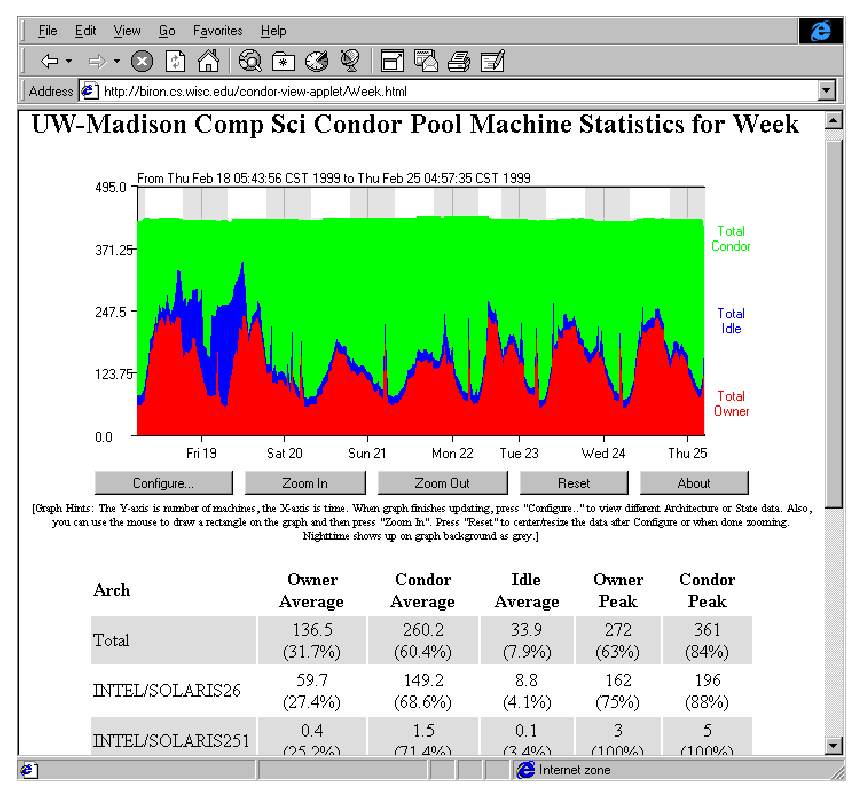
\includegraphics{contrib/view-screenshot.ps}
\caption{\label{fig:view-screenshot}Screen shot of CondorView Client}
\end{figure}

After unpacking and installing the CondorView Client, a script named
\Prog{make\_stats} can be invoked to create HTML pages displaying Condor usage
for the past hour, day, week, or month.  
By using the Unix \Prog{cron} facility to periodically execute
\Prog{make\_stats}, Condor pool usage statistics can be kept up to date
automatically.  
This simple model allows the CondorView Client to be easily installed;
no Web server CGI interface is needed.

%%%%%%%%%%%%%%%%%%%%%%%%%%%%%%%%%%%%%%%%%%%%%%%%%%%%%%%%%%%%%%%%%%%%%%
\subsection{\label{sec:condorview-client-step-by-step}
Step-by-Step Installation of the CondorView Client}
%%%%%%%%%%%%%%%%%%%%%%%%%%%%%%%%%%%%%%%%%%%%%%%%%%%%%%%%%%%%%%%%%%%%%%

\index{installation!CondorView Client}
\index{CondorView!Client installation}
\begin{enumerate}

\item Make certain that the CondorView Server is configured.
Section ~\ref{sec:Contrib-CondorView-Install}
describes configuration of the server.
The server logs information on disk in order to provide a persistent,
historical database of pool statistics.
The CondorView Client makes queries over the network to this
database.
The \Condor{collector} includes this database support.
To activate the persistent database logging, add the following entries to
the configuration file for the \Condor{collector} chosen to act as the ViewServer.
\begin{verbatim}
    POOL_HISTORY_DIR = /full/path/to/directory/to/store/historical/data 
    KEEP_POOL_HISTORY = True 
\end{verbatim}

\item Create a directory where CondorView is to place the HTML files.  
This directory should be one published by a web server, so that HTML
files which exist in this directory can be accessed using a web browser.  
This directory is referred to as the \File{VIEWDIR} directory.

\item Download the \Prog{view\_client} contrib module.
Follow links for contrib modules on the downloads page at
\URL{http://www.cs.wisc.edu/condor/downloads-v2/download.pl}.

\item Unpack or untar this contrib module into the
directory \File{VIEWDIR}.
This creates several files and subdirectories.
Further unpack the jar file within the \File{VIEWDIR} directory with:
\begin{verbatim} 
  jar -xf condorview.jar
\end{verbatim}

\item Edit the \Prog{make\_stats} script.  At the beginning of the file
are six parameters to customize.
The parameters are

        \begin{description}

	\item[\MacroNI{ORGNAME}] A brief name that identifies an
	organization. An example is ``Univ of Wisconsin''.  Do not
	use any slashes in the name or other special regular-expression
	characters. Avoid the characters \Bs \^\  and \$.

	\item[\MacroNI{CONDORADMIN}] The e-mail
	address of the Condor administrator at your site.  
	This e-mail address will appear at the bottom of the web pages.

	\item[\MacroNI{VIEWDIR}] The full path name
	(\emph{not} a relative path) to the \File{VIEWDIR} directory set
	by installation step 2.  
	It is the directory that contains the \Prog{make\_stats} script.

	\item[\MacroNI{STATSDIR}]  The full path name of the
	directory which contains the \Condor{stats} binary.
	The \Condor{stats} program is included in the \Release{bin}
	directory. 
	The value for \MacroNI{STATSDIR} is added to the \MacroNI{PATH}
	parameter by default.  

	\item[\MacroNI{PATH}] A list of subdirectories,
	separated by colons, where the \Prog{make\_stats} script can find
	the \Prog{awk}, \Prog{bc}, \Prog{sed}, \Prog{date}, and \Condor{stats}
	programs.  
	If \Prog{perl} is installed, the path should also
	include the directory where \Prog{perl} is installed.
	The following default works on most systems:
        \begin{verbatim} 
        PATH=/bin:/usr/bin:$STATSDIR:/usr/local/bin
        \end{verbatim}

        \end{description}

\item To create all of the initial HTML files, run
\begin{verbatim}
        ./make_stats setup  
\end{verbatim}
Open the file \File{index.html} to verify that things look good.

\index{CondorView!use of \Prog{crontab} program}
\index{crontab program}

\item Add the \Prog{make\_stats} program to \Prog{cron}.  
Running \Prog{make\_stats} in step 6 created a \File{cronentries} file.
This \File{cronentries} file is ready to be processed by the Unix
\Prog{crontab} command.
The \Prog{crontab} manual page contains details about
the \Prog{crontab} command and the \Prog{cron} daemon.
Look at the
\File{cronentries} file; by default, it will run 
\Prog{make\_stats} \Arg{hour} every 15 minutes, 
\Prog{make\_stats} \Arg{day} once an hour, 
\Prog{make\_stats} \Arg{week} twice per day, and 
\Prog{make\_stats} \Arg{month} once per day.
These are reasonable defaults.  
Add these commands to cron on any
system that can access the \MacroNI{VIEWDIR} and
\MacroNI{STATSDIR} directories,
even on a system that does not have Condor installed.
The commands do not need to run as root user;
in fact, they should probably not run as root.  These commands can run
as any user that has read/write access to the \File{VIEWDIR} directory.
The command
\begin{verbatim} 
  crontab cronentries
\end{verbatim}
can set the crontab file;
note that this command overwrites the current, existing crontab file with the 
entries from the file \File{cronentries}.

\item Point the web browser at the \File{VIEWDIR} directory
to complete the installation.

\end{enumerate}


%%%%%%%%%%%%%%%%%%%%%%%%%%%%%%
\section{Job Monitor/Log Viewer}
%%%%%%%%%%%%%%%%%%%%%%%%%%%%%%
\index{Job monitor}
\index{viewing!log files}

The Condor Job Monitor is a Java application designed to allow users to 
view user log files. 
It is identified as the Contrib Module called log\_viewer. 

To view a user log file, select it using the open file command in the File menu.  After the file is parsed, it will be visually represented.  Each horizontal line represents an individual job.  The x-axis
is time.  Whether a job is running at a particular time is represented by its color at that time -- white for running, black for idle.  For example, a job which appears predominantly white has made
efficient progress, whereas a job which appears predominantly black has received an inordinately small proportion of computational time. 


\subsection{\label{sec:transition-states}Transition States}

A transition state is the state of a job at any time.  It is called a "transition" because it is defined by the two events which bookmark it.  There are two basic transition states: running and idle. 
An idle job typically is a job which has just been submitted into the Condor pool and is waiting to be matched with an appropriate machine or a job which has vacated from a machine and has been
returned to the pool.  A running job, by contrast, is a job which is making active progress. 

Advanced users may want a visual distinction between two types of running transitions: "goodput" or "badput".  Goodput is the transition state preceding an eventual job completion or
checkpoint.  Badput is the transition state preceding a non-checkpointed eviction event.  Note that "badput" is potentially a misleading nomenclature; a job which is not checkpointed by the
Condor program may checkpoint itself or make progress in some other way.  To view these two transition as distinct transitions, select the appropriate option from the "View" menu. 


\subsection{\label{sec:events}Events}

There are two basic kinds of events: checkpoint events and error events.   Plus advanced users can ask to see more events. 


\subsection{\label{sec:job-selector}Selecting Jobs}

To view any arbitrary selection of jobs in a job file, use the job selector tool.  Jobs appear visually by order of appearance within the actual text log file.  For example, the log file might contain jobs
775.1, 775.2, 775.3, 775.4, and 775.5, which appear in that order.  A user who wishes to see only jobs 775.2 and 775.5 can select only these two jobs in the job selector tool and click the "Ok" or
"Apply" button.  The job selector supports double clicking; double
click on any single job to see it drawn in isolation. 

\subsection{\label{sec:zooming}Zooming}

To view a small area of the log file, zoom in on the area which you would like to see in greater detail. You can zoom in, out and do a full zoom. A full zoom redraws the log file in its entirety. For
example, if you have zoomed in very close and would like to go all the way back out, you could do so with a succession of zoom outs or with one full zoom. 

There is a difference between using the menu driven zooming and the mouse driven zooming. The menu driven zooming will recenter itself around the current center, whereas mouse driven
zooming will recenter itself (as much as possible) around the mouse click. To help you re-find the clicked area, a box will flash after the zoom. This is called the "zoom finder" and it can be turned
off in the zoom menu if you prefer. 

\subsection{\label{sec:k-m-shortcuts}Keyboard and Mouse Shortcuts}

\begin{enumerate}
\item The Keyboard shortcuts: 

\begin{itemize}
\item Arrows - an approximate ten percent scrollbar movement
\item PageUp and PageDown - an approximate one hundred percent scrollbar movement 
\item Control + Left or Right - approximate one hundred percent scrollbar movement 
\item End and Home - scrollbar movement to the vertical extreme 
\item Others - as seen beside menu items
\end{itemize}

\item The mouse shortcuts: 

\begin{itemize}
\item Control + Left click - zoom in 
\item Control + Right click - zoom out
\item Shift + left click - re-center
\end{itemize}
\end{enumerate}
 




\chapter{Version History and Release Notes}
\label{Version-History}
%%%%%%%%%%%%%%%%%%%%%%%%%%%%%%%%%%%%%%%%%%%%%%%%%%%%%%%%%%%%%%%%%%%%%%
\section{\label{sec:History-Intro}Introduction to Condor Versions}
%%%%%%%%%%%%%%%%%%%%%%%%%%%%%%%%%%%%%%%%%%%%%%%%%%%%%%%%%%%%%%%%%%%%%%

This chapter provides descriptions of what features have been added or
bugs fixed for each version of Condor.
The first section describes the Condor version numbering scheme, what
the numbers mean, and what the different \Term{release series} are.
The rest of the sections each describe a specific release series, and
all the Condor versions found in that series.

%%%%%%%%%%%%%%%%%%%%%%%%%%%%%%%%%%%%%%%%%%%%%%%%%%%%%%%%%%%%%%%%%%%%%%
\subsection{\label{sec:Version-Number-Scheme}
Condor Version Number Scheme}
%%%%%%%%%%%%%%%%%%%%%%%%%%%%%%%%%%%%%%%%%%%%%%%%%%%%%%%%%%%%%%%%%%%%%%

Starting with version 6.0.1, Condor adopted a new, hopefully easy to
understand version numbering scheme.
It reflects the fact that Condor is both a production system and a
research project.
The numbering scheme was primarily taken from the Linux kernel's
version numbering, so if you are familiar with that, it should seem
quite natural.

There will usually be two Condor versions available at any given time,
the \Term{stable} version, and the \Term{development} version.
Gone are the days of ``patch level 3'', ``beta2'', or any other random
words in the version string.
All versions of Condor now have exactly three numbers, separated by
``.''   

\begin{itemize}

\item The first number represents the major version number, and will
change very infrequently.

\item \emph{The thing that determines whether a version of Condor is
\Term{stable} or \Term{development} is the second digit.
Even numbers represent stable versions, while odd numbers represent
development versions.}

\item The final digit represents the minor version number, which
defines a particular version in a given release series.

\end{itemize}


%%%%%%%%%%%%%%%%%%%%%%%%%%%%%%%%%%%%%%%%%%%%%%%%%%%%%%%%%%%%%%%%%%%%%%
\subsection{\label{sec:Stable-Series}The Stable Release Series}
%%%%%%%%%%%%%%%%%%%%%%%%%%%%%%%%%%%%%%%%%%%%%%%%%%%%%%%%%%%%%%%%%%%%%%

People expecting the stable, production Condor system should download
the stable version, denoted with an even number in the second digit of
the version string.
Most people are encouraged to use this version.  
We will only offer our paid support for versions of Condor from the
stable release series.

\emph{On the stable series, new minor version releases will only
be made for bug fixes and to support new platforms.}
No new features will be added to the stable series.
People are encouraged to install new stable versions of Condor when
they appear, since they probably fix bugs you care about.
Hopefully, there will not be many minor version releases for any given
stable series.


%%%%%%%%%%%%%%%%%%%%%%%%%%%%%%%%%%%%%%%%%%%%%%%%%%%%%%%%%%%%%%%%%%%%%%
\subsection{\label{sec:Developement-Series}
The Development Release Series}
%%%%%%%%%%%%%%%%%%%%%%%%%%%%%%%%%%%%%%%%%%%%%%%%%%%%%%%%%%%%%%%%%%%%%%

Only people who are interested in the latest research, new features
that haven't been fully tested, etc, should download the development
version, denoted with an odd number in the second digit of the version
string.  
We will make a best effort to ensure that the development series will
work, but we make no guarantees.

On the development series, new minor version releases will probably
happen frequently.
People should not feel compelled to install new minor versions unless
they know they want features or bug fixes from the newer development
version.

\emph{Most sites will probably never want to install a development
version of Condor for any reason.}
Only if you know what you are doing (and like pain), or were
explicitly instructed to do so by someone on the Condor Team, should
you install a development version at your site.

After the feature set of the development series is satisfactory to the
Condor Team, we will put a code freeze in place, and from that point
forward, only bug fixes will be made to that development series.
When we have fully tested this version, we will release a new stable
series, resetting the minor version number, and start work on a new
development release from there.

%%%%%%%%%%%%%%%%%%%%%%%%%%%%%%%%%%%%%%%%%%%%%%%%%%%%%%%%%%%%%%%%%%%%%%
% The rest of this file just inputs other files which contain sections
% describing each release series in detail.
%%%%%%%%%%%%%%%%%%%%%%%%%%%%%%%%%%%%%%%%%%%%%%%%%%%%%%%%%%%%%%%%%%%%%%

% upgrade instructions are in the Pool Management section
%%%%%%%%%%%%%%%%%%%%%%%%%%%%%%%%%%%%%%%%%%%%%%%%%%%%%%%%%%%%%%%%%%%%%%
\section{\label{sec:gotchas}Upgrading from the 7.6 series to the 7.8 series of Condor}
%%%%%%%%%%%%%%%%%%%%%%%%%%%%%%%%%%%%%%%%%%%%%%%%%%%%%%%%%%%%%%%%%%%%%%

\index{upgrading!items to be aware of}
While upgrading from the 7.6 series of Condor to the 7.8 series will bring many
new features and improvements introduced in the 7.7 series of Condor, it will
also introduce changes that administrators of sites running from an older
Condor version should be aware of when planning an upgrade.  Here is a list of
items that administrators should be aware of.

\begin{itemize}

\item In the grid universe, the Amazon grid-type is gone and has been replaced
	with the EC2 grid-type.  Also, support for grid-type gt4 (Web Services
	GRAM) has been removed.

\item Default job submit options related to file transfers have changed. 
Across all platforms, defaults are now
\begin{verbatim}
  should_transfer_files = IF_NEEDED
  when_to_transfer_output = ON_EXIT
\end{verbatim}
See section~\ref{sec:file-transfer-if-when} for details.

\item  On Linux and Mac OS, common utility code is now contained in a set of
shared libraries. In the Linux native packages, most of these libraries
are placed under \File{/usr/lib[64]/condor} and the RUNPATH attribute is set in
the binaries to search there for them.
In the tarball packages, these libraries are placed under \File{lib} and
\File{lib/condor}, and the RUNPATH attribute is set in the binaries to search
for them under the relative paths \File{../lib} and \File{../lib/condor}.
This means that if you move or copy a Condor binary from a tarball
package to a different location, you must do one of the following:
\begin{itemize}
	\item Move or copy the corresponding \File{lib/} directory with it, or
  \item Make a symlink in the new location pointing back to the original \File{lib/}
  directory, or
  \item Set environment variable \Env{LD\_LIBRARY\_PATH} to point to the original \File{lib/} and \File{lib/condor/}
  directories
\end{itemize}
One of the new shared libraries, \File{libcondor\_utils\_7\_8\_0}, has no \File{.so}
versioning. Instead, the Condor version is included in the library name.
This means that a Condor binary must always be matched with the
\File{libcondor\_utils} library from the same Condor release.


\item  The \Condor{hdfs} service is no longer included within the Condor
	release.  Instead, the Condor + HDFS integration previously bundled with
	version 7.6 is available in version 7.8 as a \Term{Contribution Module}.
	Contribution Modules are optional packages that add functionality to
	Condor, but are provided and maintained outside of the core code base.  See
	the Condor Wiki at
	\URL{https://condor-wiki.cs.wisc.edu/index.cgi/wiki?p=ContribModules}.

\item Previous to version 7.8, by default the \Condor{master} would restart any
	individual daemon under its control if it notices that the file
	modification time of the binary for that daemon has changed.  Now the
	\Condor{master} will only monitor the file modification time of the
	\Condor{master} binary itself.  See section~\ref{sec:Pool-Upgrade}.  Also,
	see \MacroNI{MASTER\_NEW\_BINARY\_RESTART} on
	page~\pageref{param:MasterNewBinaryRestart}.

\item In DAGMan, if you have a PRE and a POST script on a node, the default now
	is that the POST script is run even if the PRE script failed.   This change
	could impact unaware workflows such that POST scripts might erroneously
	report the node as succeeded. You can get the old behavior by setting
	\MacroNI{DAGMAN\_ALWAYS\_RUN\_POST} to False.  In addition, you can no
	longer directly submit a rescue DAG file with \Condor{submit\_dag} unless
	\MacroNI{DAGMAN\_WRITE\_PARTIAL\_RESCUE} is set to False (not normally
	recommended).  See section~\ref{sec:DAGMan}.

\item The \MacroNI{KILL} expression cannot be used to grant more time to a job
	than offered by \Macro{MachineMaxVacateTime}. In Condor v7.8 and above, it
	is anticipated that most sites will simply use a default value of False for
	\MacroNI{KILL} and set \MacroNI{MachineMaxVacateTime} to control how long
	to wait.  See page~\pageref{param:MachineMaxVacateTime} for more
	information.


\end{itemize}


%%%      PLEASE RUN A SPELL CHECKER BEFORE COMMITTING YOUR CHANGES!
%%%      PLEASE RUN A SPELL CHECKER BEFORE COMMITTING YOUR CHANGES!
%%%      PLEASE RUN A SPELL CHECKER BEFORE COMMITTING YOUR CHANGES!
%%%      PLEASE RUN A SPELL CHECKER BEFORE COMMITTING YOUR CHANGES!
%%%      PLEASE RUN A SPELL CHECKER BEFORE COMMITTING YOUR CHANGES!

%%%%%%%%%%%%%%%%%%%%%%%%%%%%%%%%%%%%%%%%%%%%%%%%%%%%%%%%%%%%%%%%%%%%%%
\section{\label{sec:History-7-9}Development Release Series 7.9}
%%%%%%%%%%%%%%%%%%%%%%%%%%%%%%%%%%%%%%%%%%%%%%%%%%%%%%%%%%%%%%%%%%%%%%

This is the development release series of Condor.
The details of each version are described below.

%%%%%%%%%%%%%%%%%%%%%%%%%%%%%%%%%%%%%%%%%%%%%%%%%%%%%%%%%%%%%%%%%%%%%%
\subsection*{\label{sec:New-7-9-1}Version 7.9.1}
%%%%%%%%%%%%%%%%%%%%%%%%%%%%%%%%%%%%%%%%%%%%%%%%%%%%%%%%%%%%%%%%%%%%%%

\noindent Release Notes:

\begin{itemize}

\item Condor version 7.9.1 not yet released.
%\item Condor version 7.9.1 released on Month Date, 2012.

\item Condor no longer looks for its main configuration file in the
location \File{\MacroUNI{GLOBUS\_LOCATION}/etc/condor\_config}.
\Ticket{2830}

\end{itemize}


\noindent New Features:

\begin{itemize}

\item \Condor{job\_router} can now submit the routed copy of jobs to a
different \Condor{schedd} than the one that serves as the source of
jobs to be routed.  The spool directories of the two
\Condor{schedds} must still be directly accessible to
\Condor{job\_router}.  This feature is enabled by using the new
optional configuration settings:

\begin{itemize}
\item \Macro{JOB\_ROUTER\_SCHEDD1\_SPOOL}
\item \Macro{JOB\_ROUTER\_SCHEDD2\_SPOOL}
\item \Macro{JOB\_ROUTER\_SCHEDD1\_NAME}
\item \Macro{JOB\_ROUTER\_SCHEDD2\_NAME}
\item \Macro{JOB\_ROUTER\_SCHEDD1\_POOL}
\item \Macro{JOB\_ROUTER\_SCHEDD2\_POOL}
\end{itemize}
\Ticket{3030}

\item \Condor{defrag} now has a policy option to cancel draining
of a machine that is in draining mode.  This can be used to effect
partial draining of machines.
\Ticket{2993}

\end{itemize}

\noindent Configuration Variable and ClassAd Attribute Additions and Changes:

\begin{itemize}

\item Added the attribute \Attr{DAGManNodesMask} to control the verboseness of
the log referred to by \Attr{DAGManNodesLog}.

\item The new configuration variable
\Macro{QUEUE\_SUPER\_USER\_MAY\_IMPERSONATE} specifies a regular
expression that matches the user names that
the queue super user may impersonate when managing jobs.  When not
set, the default behavior is to allow impersonation of any user who
has had a job in the queue during the life of the \Condor{schedd}.  For
proper functioning of the \Condor{shadow}, the \Condor{gridmanager}, and
the \Condor{job\_router}, this expression, if set, must match the owner
names of all jobs that these daemons will manage.
\Ticket{3030}

\label{JobRouterSchedd1Spool}
\item[\Macro{JOB\_ROUTER\_SCHEDD1\_SPOOL}]
  The path to the spool directory for the \Condor{schedd} serving as the
  source of jobs for routing.  If not specified, this defaults to
  \Macro{SPOOL}.  If specified, this parameter must point to the spool
  directory of the \Condor{schedd} identified by \Macro{JOB\_ROUTER\_SCHEDD1\_NAME}.

\label{JobRouterSchedd2Spool}
\item[\Macro{JOB\_ROUTER\_SCHEDD2\_SPOOL}]
  The path to the spool directory for the \Condor{schedd} to which the
  routed copy of the jobs are submitted.  If not specified, this defaults to
  \Macro{SPOOL}.  If specified, this parameter must point to the spool
  directory of the \Condor{schedd} identified by \Macro{JOB\_ROUTER\_SCHEDD2\_NAME}.

\label{JobRouterSchedd1Name}
\item[\Macro{JOB\_ROUTER\_SCHEDD1\_NAME}]
  The advertised daemon name of the \Condor{schedd} serving as the
  source of jobs for routing.  If not specified, this defaults to the
  local \Condor{schedd}.  If specified, this parameter must name the
  same \Condor{schedd} whose spool is configured in
  \Macro{JOB\_ROUTER\_SCHEDD1\_SPOOL}.  If the named \Condor{schedd} is
  not advertised in the local pool, \Macro{JOB\_ROUTER\_SCHEDD1\_POOL}
  will also need to be set.

\label{JobRouterSchedd2Name}
\item[\Macro{JOB\_ROUTER\_SCHEDD2\_NAME}]
  The advertised daemon name of the \Condor{schedd} to which the
  routed copy of the jobs are submitted.  If not specified, this defaults to
  the local \Condor{schedd}.  If specified, this parameter must name the
  same \Condor{schedd} whose spool is configured in
  \Macro{JOB\_ROUTER\_SCHEDD2\_SPOOL}.  If the named \Condor{schedd} is
  not advertised in the local pool, \Macro{JOB\_ROUTER\_SCHEDD2\_POOL}
  will also need to be set.

\label{JobRouterSchedd1Pool}
\item[\Macro{JOB\_ROUTER\_SCHEDD1\_POOL}]
  The Condor pool (collector address) of the \Condor{schedd} serving as the
  source of jobs for routing.  If not specified, this defaults to the
  local pool.

\label{JobRouterSchedd2Pool}
\item[\Macro{JOB\_ROUTER\_SCHEDD2\_POOL}]
  The Condor pool (collector address) of the \Condor{schedd} to which
  the routed copy of the jobs are submitted.  If not specified, this
  defaults to the local pool.

\label{JobRouterSchedd2Pool}
\item[\Macro{DEFRAG\_WHOLE\_MACHINE\_EXPR}]
  This new configuration value is an expression that specifies
  which draining machines should have draining be canceled.  This defaults
  to \Macro{DEFRAG\_WHOLE\_MACHINE\_EXPR}.  This could be used to drain
  partial rather than whole machines.
\Ticket{2993}

\end{itemize}

\noindent Bugs Fixed:

\begin{itemize}

\item The ClassAd functions \Procedure{splitUserName} and \Procedure{splitSlotName}
leaked a small amount of memory every time they were evaluated.  This bug was
introduced when these functions were added in 7.7.6.
\Ticket{3082}

\end{itemize}

\noindent Known Bugs:

\begin{itemize}

\item None.

\end{itemize}

\noindent Additions and Changes to the Manual:

\begin{itemize}

\item None.

\end{itemize}


%%%%%%%%%%%%%%%%%%%%%%%%%%%%%%%%%%%%%%%%%%%%%%%%%%%%%%%%%%%%%%%%%%%%%%
\subsection*{\label{sec:New-7-9-0}Version 7.9.0}
%%%%%%%%%%%%%%%%%%%%%%%%%%%%%%%%%%%%%%%%%%%%%%%%%%%%%%%%%%%%%%%%%%%%%%

\noindent Release Notes:

\begin{itemize}

\item Condor version 7.9.0 not yet released.
%\item Condor version 7.9.0 released on Month Date, 2012.

\end{itemize}


\noindent New Features:

\begin{itemize}

\item Machine slots can now be configured to identify and
divide customized local resources.
Jobs may then request these resources.
See section~\ref{sec:Configuring-SMP} for details.
\Ticket{2905}

\item Condor now supports and implements the caching of ClassAds 
to reduce memory footprints. Caching may be disabled by setting
the new configuration variable \Macro{ENABLE\_CLASSAD\_CACHING}
to \Expr{False}.
Third party use of the ClassAd library does not enable the
caching of ClassAds by default; 
Condor does enable the caching of ClassAds by default.
\Ticket{2541}
\Ticket{3127}

\item \Condor{status} now returns the \Condor{schedd} ClassAd directly 
from the \Condor{schedd} daemon,
if both options \Opt{-direct} and \Opt{-schedd} are given on the command line.
\Ticket{2492}

\item The new \Opt{-status} and \Opt{-echo} command line options to 
\Condor{wait} command cause it to show job start and terminate information,
and to print events to \Code{stdout}.
\Ticket{2926}

\item Added a \Expr{DEBUG} logging level output flag \Dflag{CATEGORY},
which causes Condor to include the logging level
flags in effect for each line of logged output.
\Ticket{2712}

\item \Condor{status} and \Condor{q} each have a new \Opt{-autoformat} option
to make some output format specifications easier than the existing
\Opt{-format} option.
See the \Condor{status} manual page located on page~\pageref{man-condor-status}
and the \Condor{q} manual page located on page~\pageref{man-condor-q} 
for details.
\Ticket{2941}

\item Enhanced the ClassAd log system to report the log line number 
on parse failures, 
and improved the ability to detect parse failures closer to 
the point of corruption.
\Ticket{2934}

\item Added an \Opt{-evaluate} option to \Condor{config\_val}, which causes the configured value queried from
a given daemon to be evaluated with respect to that daemon's ClassAd.
\Ticket{856}

\item Added code to \Condor{dagman},
such that a \Expr{VARS} assignment in a top-level DAG is applied to splices.
\Ticket{1780}

\item Condor now uses libraries from Globus 5.2.1.
\Ticket{2838}

\item When authenticating Condor daemons with GSI and
configuration variable \MacroNI{GSI\_DAEMON\_NAME} is undefined, 
Condor checks that the server name in the certificate matches the 
host name that the client is connecting to. 
When \MacroNI{GSI\_DAEMON\_NAME} is defined,
the old behavior is preserved: only certificates matching
\MacroNI{GSI\_DAEMON\_NAME} pass the authentication step, 
and no host name check is performed.  
The behavior of the host name check
may be further controlled with the new configuration variables
\MacroNI{GSI\_SKIP\_HOST\_CHECK} and
\MacroNI{GSI\_SKIP\_HOST\_CHECK\_CERT\_REGEX}.
\Ticket{1605}

\item Added new capability to \Condor{submit} to allow recursive macros in
submit description files. 
This facility allows one to update variables recursively. 
Before this new capability was added,
recursive definition would send \Condor{submit} into an
infinite loop of expanding the macro,
such that the expansion would fill up memory.
See section~\ref{macro-in-submit-description-file} for details.
\Ticket{406}

\item A DAGMan limitation and restriction has been removed.  
It is now permitted to define a \SubmitCmd{log} command using a macro,
within a node job's submit description file.
\Ticket{2428}

\item To enforce the dependencies of a DAG,
DAGMan now uses and watches only the default node
user log of the \Condor{dagman} job for events.  
DAGMan requests the \Condor{schedd} and \Condor{shadow} daemons to write each
event to this default log, 
in addition to writing to a log specified by the node job.
\Condor{dagman} writes POST script terminate events only to its default log;
these terminate events are not written to the user log.
This behavior can be turned off by setting the configuration variable
\Macro{DAGMAN\_ALWAYS\_USE\_NODE\_LOG} to \Expr{False}.
For correct behavior,
\MacroNI{DAGMAN\_ALWAYS\_USE\_NODE\_LOG} should be set to \Expr{False}
if \Condor{dagman} version 7.9.0 or later is submitting jobs 
to an older version of
a \Condor{schedd} daemon or of a \Condor{submit} executable.
\Ticket{2807}

\end{itemize}

\noindent Configuration Variable and ClassAd Attribute Additions and Changes:

\begin{itemize}

\item The new configuration variables \Macro{MACHINE\_RESOURCE\_NAMES}
(see section~\ref{param:MachineResourceNames})
and \Macro{MACHINE\_RESOURCE\_<name>}
(see section~\ref{param:MachineResourceResourcename})
identify and specify the use of customized local machine resources.
\Ticket{2905}

\item The new configuration variable \MacroNI{ENABLE\_CLASSAD\_CACHING}
controls whether the new caching feature of ClassAds is used.
The default value is \Expr{True}.
\Ticket{3127}

\item The new configuration variable \Macro{CLASSAD\_LOG\_STRICT\_PARSING}
controls whether ClassAd log files such as the job queue
log are read with strict parse checking on ClassAd expressions.
\Ticket{3069}

\item The default value for configuration variable \Macro{USE\_PROCD}
is now \Expr{True} for the \Condor{master} daemon.  
This means that by
default the \Condor{master} will start a \Condor{procd} daemon to be used 
by it and all other daemons on that machine.
\Ticket{2911}

\item There is a new configuration variable used by the \Condor{starter}.
If \Macro{STARTER\_RLIMIT\_AS} is set to an integer value, 
the \Condor{starter}
will use the \Procedure{setrlimit} system call with the 
\Code{RLIMIT\_AS} parameter to
limit the virtual memory size of each process in the user job.  
The value of this configuration variable is a ClassAd expression, 
evaluated in the context of both the machine and job ClassAds, 
where the machine ClassAd is the \Expr{my} ClassAd, 
and the job ClassAd is the \Expr{target} ClassAd.
\Ticket{1663}

\item New configuration variables were added to to the \Condor{schedd} to
define statistics that count subsets of jobs. 
These variables have the form \Macro{SCHEDD\_COLLECT\_STATS\_BY\_<Name>},
and should be defined by a ClassAd expression that evaluates to a string.
See section~\ref{param:ScheddCollectStatsByName}
for the complete definition.
The optional configuration variable of the form
\Macro{SCHEDD\_EXPIRE\_STATS\_BY\_<Name>} can be used to set an expiration time,
in seconds, for each set of statistics.
\Ticket{2862}

\item The new \SubmitCmd{batch\_queue} submit description file command
and new job ClassAd attribute \Attr{BatchQueue} specify which job
queue to use for grid universe jobs of type
\SubmitCmd{pbs}, \SubmitCmd{lsf}, and \SubmitCmd{sge}.
\Ticket{2996}

\item The new configuration variable \Macro{GSI\_SKIP\_HOST\_CHECK} is
a boolean that controls whether a check is performed during
GSI authentication of a Condor daemon.  
When the default value \Expr{False},
the check is not skipped, so the daemon host name must match the
host name in the daemon's certificate, unless otherwise exempted
by values of \MacroNI{GSI\_DAEMON\_NAME} or
\MacroNI{GSI\_SKIP\_HOST\_CHECK\_CERT\_REGEX}.
When \Expr{True}, this check is skipped, and hosts will not be rejected
due to a mismatch of certificate and host name.
\Ticket{1605}

\item The new configuration variable
\MacroNI{GSI\_SKIP\_HOST\_CHECK\_CERT\_REGEX} may be set to a
regular expression.  GSI certificates of Condor daemons with a
subject name that are matched in full by this regular expression
are not required to have a matching daemon host name and certificate
host name.  The default is an empty regular expression, which will
not match any certificates, even if they have an empty subject name.
\Ticket{1605}

\end{itemize}

\noindent Bugs Fixed:

\begin{itemize}

\item Fixed a bug in which usage of cgroups incorrectly included the page cache 
in the maximum memory usage.
This bug fix is also included in Condor version 7.8.2.
\Ticket{3003}

\item The EC2 GAHP will now respect the value of the environment variable
\Env{X509\_CERT\_DIR} and the configuration variable
\Macro{GSI\_DAEMON\_TRUSTED\_CA\_DIR} for \emph{all} secure connections.
\Ticket{2823}

\item Condor will avoid selecting down (disabled) network interfaces.  Previously Condor could select a down interface over an up (active) interface.
\Ticket{2893}

\item Made logic in the \Condor{negotiator} that computes submitter limits 
properly aware of the configuration variable
\Macro{NEGOTIATOR\_CONSIDER\_PREEMPTION}.
\Ticket{2952}


\item Condor no longer back-dates file modification times by 3 minutes
when transferring job input files into the job spool directory or the job
execute directory.
\Ticket{2423}

\item Fixed a bug in which the use of a pipe in the configuration file 
on Windows platforms would cause a visible console window 
to show up whenever the configuration was read.
\Ticket{1534}

\end{itemize}

\noindent Known Bugs:

\begin{itemize}

\item None.

\end{itemize}

\noindent Additions and Changes to the Manual:

\begin{itemize}

\item Machine ClassAd attribute string values relating to \Attr{OpSys} have
been documented for Scientific Linux platforms.
\Ticket{2366}

\end{itemize}



%%%      PLEASE RUN A SPELL CHECKER BEFORE COMMITTING YOUR CHANGES!
%%%      PLEASE RUN A SPELL CHECKER BEFORE COMMITTING YOUR CHANGES!
%%%      PLEASE RUN A SPELL CHECKER BEFORE COMMITTING YOUR CHANGES!
%%%      PLEASE RUN A SPELL CHECKER BEFORE COMMITTING YOUR CHANGES!
%%%      PLEASE RUN A SPELL CHECKER BEFORE COMMITTING YOUR CHANGES!

%%%%%%%%%%%%%%%%%%%%%%%%%%%%%%%%%%%%%%%%%%%%%%%%%%%%%%%%%%%%%%%%%%%%%%
\section{\label{sec:History-7-8}Stable Release Series 7.8}
%%%%%%%%%%%%%%%%%%%%%%%%%%%%%%%%%%%%%%%%%%%%%%%%%%%%%%%%%%%%%%%%%%%%%%

This is a stable release series of Condor.
As usual, only bug fixes (and potentially, ports to new platforms)
will be provided in future 7.8.x releases.
New features will be added in the 7.9.x development series.

The details of each version are described below.

%%%%%%%%%%%%%%%%%%%%%%%%%%%%%%%%%%%%%%%%%%%%%%%%%%%%%%%%%%%%%%%%%%%%%%
\subsection*{\label{sec:New-7-8-2}Version 7.8.2}
%%%%%%%%%%%%%%%%%%%%%%%%%%%%%%%%%%%%%%%%%%%%%%%%%%%%%%%%%%%%%%%%%%%%%%

\noindent Release Notes:

\begin{itemize}

\item Condor version 7.8.2 not yet released.
%\item Condor version 7.8.2 released on Month Date, 2012.

\end{itemize}


\noindent New Features:

\begin{itemize}

\item The \File{libcondorapi} library for reading and writing job event
logs is again available as a shared library on Linux and Mac OS platforms.
Since Condor 7.5.x, it had only been available as a static library.
\Ticket{3047}

\end{itemize}

\noindent Configuration Variable and ClassAd Attribute Additions and Changes:

\begin{itemize}

\item To avoid the output of an unnecessary DAGMan error message,
the value of \Macro{DAGMAN\_LOG\_ON\_NFS\_IS\_ERROR}
is ignored when both \MacroNI{CREATE\_LOCKS\_ON\_LOCAL\_DISK}
and \MacroNI{ENABLE\_USERLOG\_LOCKING} are \Expr{True}.
\Ticket{3087}

\end{itemize}

\noindent Bugs Fixed:

\begin{itemize}

\item Fixed a bug in which usage of cgroups incorrectly included the
page cache in the maximum memory usage.
This bug fix is also included in Condor version 7.9.0.
\Ticket{3003}

\item Jobs from a hook to fetch work, 
where the hook is defined by configuration variable 
\MacroNI{<Keyword>\_HOOK\_FETCH\_WORK},
now correctly receive dynamic slots from a partitionable slot 
instead of claiming the entire partitionable slot.
\Ticket{2819}

\item Fixed a bug in which a slot might become stuck in the Preempting state
when a \Condor{startd} is configured with a hook to fetch work,
as defined by \Macro{<Keyword>\_HOOK\_FETCH\_WORK}.
\Ticket{3076}

\item Fixed a bug that caused Condor to transfer a job's input files from
the execute machine back to the submit machine as if they were output files.
This would happen if the
job's input files were stored in Condor's spool directory;
occurred if the job was submitted via Condor-C or via 
\Condor{submit} with the \Opt{-spool} or \Opt{-remote} options.
\Ticket{2406}

\item Fixed a bug that could cause the first grid-type cream jobs destined 
for a particular CREAM server to never be submitted to that server.
This bug was probably introduced in Condor version 7.6.5.
\Ticket{3054}

\item Fixed several problems with the XML parsing class
\Code{ClassAdXMLParser} in the ClassAds library:
  \begin{itemize}
  \item Several methods named \Procedure{ParseClassAd} were declared, 
  but never implemented. 
\Ticket{3049}
  \item The parser silently dropped leading white space in string values.
\Ticket{3042}
  \item The parser could go into an infinite loop or leak memory when
    reading a malformed ClassAd XML document. 
\Ticket{3045}
  \end{itemize}

\item Fixed a bug that prevented the \Opt{-f} command line option to
\Condor{history} from being recognized.
The \Opt{-f} option was being interpreted as \Opt{-forward}. 
At least four letters are now required for the \Opt{-forward} option
(\Opt{-forw}) to prevent ambiguity.
\Ticket{3044}

\item The implementation of the \Condor{history} \Opt{-backwards} option, 
which is the default ordering for reading the history file,
in the 7.7 series did not work on Windows platforms.
This has been fixed.
\Ticket{3055}

\item Fixed a bug that caused an invalid proxy to be delegated when
refreshing the job's X.509 proxy when configuration variable
\Macro{DELEGATE\_JOB\_GSI\_CREDENTIALS\_LIFETIME} was set to 0.
\Ticket{3059}

\item Fixed a bug in which DAGMan did not account properly for jobs being
suspended and then unsuspended.
\Ticket{3108}

\item Job IDs generated by NorduGrid ARC 12.05 and above are now
properly recognized.
\Ticket{3062}

\item Fixed a bug in which Condor would not mark grid-type nordugrid jobs
as Running due to variation in the format of the job status value.
NorduGrid ARC job statuses of the form \Expr{INLRMS: ?} are now
properly recognized both with and without the space after the colon.
\Ticket{3118}

\item The \Condor{gridmanager} now properly handles X.509 proxy files
that are specified in the job ClassAd with a relative path name.
\Ticket{3027}

\item Fixed a bug that caused daemon names,
as set in configuration variables such as \MacroNI{STARTD\_NAME},
containing a period character to be ignored.
\Ticket{3172}

\item Fixed a bug that prevented the \Condor{schedd} from removing old
execute directories for local universe jobs on startup.
\Ticket{3176}

\item \Condor{dagman} now takes note of \Macro{ULOG\_JOB\_RECONNECT\_FAILED} 
events in the user log for counting idle jobs.
\Ticket{3189}

\end{itemize}

\noindent Known Bugs:

\begin{itemize}

\item None.

\end{itemize}

\noindent Additions and Changes to the Manual:

\begin{itemize}

\item None.

\end{itemize}


%%%%%%%%%%%%%%%%%%%%%%%%%%%%%%%%%%%%%%%%%%%%%%%%%%%%%%%%%%%%%%%%%%%%%%
\subsection*{\label{sec:New-7-8-1}Version 7.8.1}
%%%%%%%%%%%%%%%%%%%%%%%%%%%%%%%%%%%%%%%%%%%%%%%%%%%%%%%%%%%%%%%%%%%%%%

\noindent Release Notes:

\begin{itemize}

\item Condor version 7.8.1 released on June 15, 2012.

\end{itemize}


\noindent New Features:

\begin{itemize}

\item None.

\end{itemize}

\noindent Configuration Variable and ClassAd Attribute Additions and Changes:

\begin{itemize}

\item (Added in 7.8.0.) The new configuration variable
\Macro{ENABLE\_DEPRECATION\_WARNINGS} causes \Condor{submit} to issue
warnings when a job requests features that are no longer supported.
\Ticket{2968}

\item (Added in 7.7.6) The new configuration variable
\Macro{BATCH\_GAHP} should be used instead of \Macro{PBS\_GAHP},
\Macro{LSF\_GAHP} and \Macro{SGE\_GAHP}. These older configuration
variables are still recognized, but their use is now discouraged.
\Ticket{2670}

\item The default value for \Macro{GROUP\_SORT\_EXPR} was changed 
so that the \Expr{<none>} group would always negotiate last 
when using hierarchical group quotas.
Associated with that, 
the default value for \Macro{NEGOTIATOR\_ALLOW\_QUOTA\_OVERSUBSCRIPTION} 
was changed to \Expr{True}.  
These changes were made to make negotiation behave more like it did 
in the stable 7.4 series of Condor,
before hierarchical group quotas were added.
\Ticket{3040}

\end{itemize}

\noindent Bugs Fixed:

\begin{itemize}

\item Fixed a bug that caused events to not be written to the job event
log when the log is written in XML and a job policy expression triggering
the event contains any double quote marks.
\Ticket{3048}

\item Fixed a bug in the Condor init script that would cause
the init script to hang if Condor was not running.
\Ticket{2872}

\item Fixed a bug that caused parallel universe jobs using
Parallel Scheduling Groups 
(see section ~\ref{sec:Configure-Dedicated-Groups})
to occasionally stay idle even when
there were available machines to run them.
\Ticket{3017}

\item Fixed a bug that caused the \Condor{gridmanager} to crash when
attempting to submit jobs to a local PBS, LSF, or SGI cluster.
\Ticket{3014}

\item Fixed a bug in the handling of local universe jobs which caused
the \Condor{schedd} to log a spurious \Expr{ERROR} message
every time a local universe job exited, 
and then further caused the statistics for local universe jobs to be 
incorrectly computed.
\Ticket{3008}

\item Changed the internally used \Condor{ckpt\_probe} executable
to link statically, which should make the
checkpoint signature more resistant to non-significant changes in the system
configuration.
\Ticket{2901}

\item Restored Globus and VOMS support for the Mac OS X platform.
\Ticket{2991}

\item Fixed a bug when Condor runs under the PrivSep model,
in which if a job created a hard link from one file to another,
Condor was unable to transfer the files back to the submit side,
and the job was put on hold.
\Ticket{2987}

\item When configuration variables \MacroNI{MaxJobRetirementTime} or
\MacroNI{MachineMaxVacateTime} were very large, estimates of machine
draining badput and completion time were sometimes nonsensical
because of integer overflow.
\Ticket{3001}

\item Fixed a bug where per-job subdirectories and their contents
in \MacroUNI{SPOOL} would not be removed when the associated job
left the queue.
\Ticket{2942}

\item Fixed a bug that could cause the \Condor{schedd} to 
occasionally crash due to a race condition when running local universe jobs.
Associated with the bug would be the error message
\footnotesize
\begin{verbatim}
No local universe jobs were expected to be running, but one just exited!
\end{verbatim}
\normalsize
\Ticket{3009}

\end{itemize}

\noindent Known Bugs:

\begin{itemize}

\item None.

\end{itemize}

\noindent Additions and Changes to the Manual:

\begin{itemize}

\item Submit description file commands introduced in Condor version 7.7.1
have now been documented.
See the \Condor{submit} manual page at ~\ref{man-condor-submit} for
the newly added definitions of
\begin{description}
  \item[\SubmitCmd{ec2\_availability\_zone}]
  \item[\SubmitCmd{ec2\_ebs\_volumes}]
  \item[\SubmitCmd{ec2\_elastic\_ip}]
  \item[\SubmitCmd{ec2\_keypair\_file}]
  \item[\SubmitCmd{ec2\_vpc\_ip}]
  \item[\SubmitCmd{ec2\_vpc\_subnet}]
\end{description}

\item There is now a manual page for \Condor{router\_rm}, 
a script that provides additional features convenient for removing
jobs managed by the Condor Job Router.

\item Documentation not completed for the 7.7.6 release is now available.
The use of configuration variable \MacroNI{BATCH\_GAHP},
as well as the use of the new \SubmitCmd{grid\_resource} of
type \Expr{batch} for local submission of PBS, LSF, and SGE
jobs is documented.
See section ~\ref{sec:batch} for details.
\Ticket{2670}

\end{itemize}


%%%%%%%%%%%%%%%%%%%%%%%%%%%%%%%%%%%%%%%%%%%%%%%%%%%%%%%%%%%%%%%%%%%%%%
\subsection*{\label{sec:New-7-8-0}Version 7.8.0}
%%%%%%%%%%%%%%%%%%%%%%%%%%%%%%%%%%%%%%%%%%%%%%%%%%%%%%%%%%%%%%%%%%%%%%

\noindent Release Notes:

\begin{itemize}

\item Condor version 7.8.0 released on May 10, 2012.

\end{itemize}


\noindent New Features:

\begin{itemize}

\item (Added in 7.7.6.)  The new \Arg{-\_condor\_relocatable} argument
may be given as part of the invocation of a program that uses
standalone checkpointing.  This allows checkpointed programs to restart
without attempting to change to their original directory.
\Ticket{2877}

\item (Added in 7.7.5.) Added the \Arg{-absent} flag to \Condor{status},
which displays absent ClassAds.
\Ticket{2690}

\item (Added in 7.7.5.) Implement absent ads, which help track pool membership
in a persistent way.
\Ticket{2608} 

\end{itemize}

\noindent Configuration Variable and ClassAd Attribute Additions and Changes:

\begin{itemize}

\item The job ClassAd attribute \Attr{RemotePool} is now saved in
  \Attr{LastRemotePool} when the job finishes running.

\end{itemize}

\noindent Bugs Fixed:

\begin{itemize}

\item (Fixed in 7.7.6.) Fix \Arg{-absent}, \Arg{-vm}, and \Arg{-java}
flags to \Condor{status} so that they work with the \Arg{-long} option.
\Ticket{2943}

\item Support glob() on Scientific Linux 6 and others using the new
Linux system call fstatat(), but only when not using remote system calls.
\Ticket{2945}

\item Fixed potential startd crash introduced in v7.7.5 when claiming 
a partitionable slot that was in the Owner state. 
\Ticket{2936}

\item When ClassAd function stringListMember() is called with an empty
string as the second argument, it now evaluates to \Expr{False}.
Previously, it incorrectly evaluated to \Expr{Undefined}.
\Ticket{2953}

\item Format tags \%v and \%V for the \Opt{-format} option now properly
print all ClassAd value types. Previously, \Expr{True} and \Expr{False}
were printed as integers, and new ClassAd types like lists and nested
ClassAds could not be printed.
\Ticket{2960}

\item Restored RCS keyword strings CondorVersion and CondorPlatform to
the Condor binaries. These strings are found and printed by the 
\Opt{ident} program on Unix. They were missing in Condor versions 7.7.3
and later.
\Ticket{2932}

\item \Condor{job\_router} failed to route spooled source jobs.
\Ticket{2955}

\item Fixed a bug on Debian 6 and RHEL 6 that could cause standard
universe jobs to never checkpoint. This would happen if the job
triggered a call to NSCD (Name Service Caching Daemon) but NSCD 
wasn't running. 
Calls to NSCD can be triggered by a look up of a user account or
resolving a machine hostname to an IP address.
Now, NSCD is never consulted by a standard universe
job (this was already the behavior on other platforms).
\Ticket{2973}

\end{itemize}

\noindent Known Bugs:

\begin{itemize}

\item None.

\end{itemize}

\noindent Additions and Changes to the Manual:

\begin{itemize}

\item None.

\end{itemize}



%%%      PLEASE RUN A SPELL CHECKER BEFORE COMMITTING YOUR CHANGES!
%%%      PLEASE RUN A SPELL CHECKER BEFORE COMMITTING YOUR CHANGES!
%%%      PLEASE RUN A SPELL CHECKER BEFORE COMMITTING YOUR CHANGES!
%%%      PLEASE RUN A SPELL CHECKER BEFORE COMMITTING YOUR CHANGES!
%%%      PLEASE RUN A SPELL CHECKER BEFORE COMMITTING YOUR CHANGES!

%%%%%%%%%%%%%%%%%%%%%%%%%%%%%%%%%%%%%%%%%%%%%%%%%%%%%%%%%%%%%%%%%%%%%%
\section{\label{sec:History-7-7}Development Release Series 7.7}
%%%%%%%%%%%%%%%%%%%%%%%%%%%%%%%%%%%%%%%%%%%%%%%%%%%%%%%%%%%%%%%%%%%%%%

This is the development release series of Condor.
The details of each version are described below.


%%%%%%%%%%%%%%%%%%%%%%%%%%%%%%%%%%%%%%%%%%%%%%%%%%%%%%%%%%%%%%%%%%%%%%
\subsection*{\label{sec:New-7-7-5}Version 7.7.5}
%%%%%%%%%%%%%%%%%%%%%%%%%%%%%%%%%%%%%%%%%%%%%%%%%%%%%%%%%%%%%%%%%%%%%%

\noindent Release Notes:

\begin{itemize}

\item Condor version 7.7.5 not yet released.
%\item Condor version 7.7.5 released on Month Date, 2011.

\end{itemize}


\noindent New Features:

\begin{itemize}

\item  \Condor{q} \Opt{-run} now displays the value of the job ClassAd
attribute \Attr{EC2RemoteVirtualMachineName} instead of
\Expr{[????????????????]},
under the HOST(S) column for grid type ec2 jobs.
\Ticket{2599}

\end{itemize}

\noindent Configuration Variable and ClassAd Attribute Additions and Changes:

\begin{itemize}

\item The new configuration variable \Macro{JOB\_QUEUE\_LOG} 
specifies an alternative path and file name for the \File{job\_queue.log} file.
The default value is \File{\MacroUNI{SPOOL}/job\_queue.log}.
This alternative location can be
useful if there is a solid state drive which is big enough to hold the
frequently written to \File{job\_queue.log},
but not big enough to hold the whole contents of the spool directory.
\Ticket{2598}

\end{itemize}

\noindent Bugs Fixed:

\begin{itemize}

\item Communication errors were not always correctly handled when
fetching results of a query when using the \Opt{-stream} option to
\Condor{q}.  This problem was introduced in 7.7.0.
\Ticket{2601}

\end{itemize}

\noindent Known Bugs:

\begin{itemize}

\item None.

\end{itemize}

\noindent Additions and Changes to the Manual:

\begin{itemize}

\item None.

\end{itemize}


%%%%%%%%%%%%%%%%%%%%%%%%%%%%%%%%%%%%%%%%%%%%%%%%%%%%%%%%%%%%%%%%%%%%%%
\subsection*{\label{sec:New-7-7-4}Version 7.7.4}
%%%%%%%%%%%%%%%%%%%%%%%%%%%%%%%%%%%%%%%%%%%%%%%%%%%%%%%%%%%%%%%%%%%%%%

\noindent Release Notes:

\begin{itemize}

\item Condor version 7.7.4 not yet released.
%\item Condor version 7.7.4 released on Month Date, 2011.

\end{itemize}


\noindent New Features:

\begin{itemize}

\item None.

\end{itemize}

\noindent Configuration Variable and ClassAd Attribute Additions and Changes:

\begin{itemize}

\item None.

\end{itemize}

\noindent Bugs Fixed:

\begin{itemize}

\item None.

\end{itemize}

\noindent Known Bugs:

\begin{itemize}

\item None.

\end{itemize}

\noindent Additions and Changes to the Manual:

\begin{itemize}

\item None.

\end{itemize}


%%%%%%%%%%%%%%%%%%%%%%%%%%%%%%%%%%%%%%%%%%%%%%%%%%%%%%%%%%%%%%%%%%%%%%
\subsection*{\label{sec:New-7-7-3}Version 7.7.3}
%%%%%%%%%%%%%%%%%%%%%%%%%%%%%%%%%%%%%%%%%%%%%%%%%%%%%%%%%%%%%%%%%%%%%%

\noindent Release Notes:

\begin{itemize}

\item Condor version 7.7.3 not yet released.
%\item Condor version 7.7.3 released on Month Date, 2011.

\item
\emph{Condor now dynamically links with the ClassAds, Globus and VOMS
libraries on Mac OS X.}
A copy of these libraries is included with Condor.
\Ticket{2482}

\end{itemize}


\noindent New Features:

\begin{itemize}

\item In Condor version 7.7.2, multiple Condor installations led to the
possibility for some installations to use the wrong version of the ClassAds 
library.
This should no longer be an issue, 
as the binaries now use \Env{RUNPATH} instead of \Env{RPATH}, 
allowing use of the \Env{LD\_LIBRARY\_PATH} environment variable 
to set where to look for the shared libraries.
\Ticket{2539}

\item The Amazon SOAP interface is no longer present or supported in Condor.
The EC2 REST interface is favored and supported in Condor
using a \SubmitCmd{grid\_resource} of \SubmitCmd{ec2}.
\Ticket{2523}

\item The new \Condor{gather\_info} tool introduced in 
Condor version 7.5.6 has been updated and enhanced.
It collects data about a Condor installation, and, if desired, 
about a specific job. 
This information is useful to Condor developers to help 
debug problems in a pool or with a job.
\Ticket{1664}
\Ticket{2372}

\item The \Condor{userprio} tool supports two new command line options.
The \Opt{-grouporder} flag displays submitter entries 
for accounting groups at top of the list,
 in breadth-first order by group hierarchy.
The \Opt{-grouprollup} flag reports accounting statistics for groups 
as summed at a level within the group hierarchy.
\Ticket{1926}

\item The \Condor{collector} now avoids the performance problems caused
previously when clients initiated communication with the \Condor{collector},
but then delayed sending input.
\Ticket{2506}

\item When using versions of \Prog{glexec} that create a copy of the proxy 
for use by the job, 
Condor now ensures that this copy of the proxy is cleaned up
when the job is done.
\Ticket{2501}

\item The \Condor{startd} now logs a clear message, if it rejects a job
because no valid \Condor{starter} daemons were detected.
\Ticket{2470}

\item The new submit command \SubmitCmd{want\_graceful\_removal}
may be used to specify that a job being removed or put on hold should
be shut down gracefully, rather than being immediately hard-killed.
This allows the job to perform some final actions such as cleaning
up or saving state.  The usual policies governing the Preempting/Vacating
state apply in this case.  

This new submit command replaces a different mechanism that was added 
in Condor version 7.5.2 to achieve some of the same effects.  
The version 7.5.2 mechanism applied to vanilla jobs under Linux;
if the job set \SubmitCmd{remove\_kill\_sig} or \SubmitCmd{kill\_sig},
the hard-kill signal that Condor would normally send to end the job was
replaced with the signal specified by the user.  

With the new submit command, the version 7.5.2 mechanism is no longer used.
The soft-kill signal may still be customized using
\SubmitCmd{kill\_sig}, so a similar effect can be achieved by setting
\Expr{want\_graceful\_removal=True} and setting \SubmitCmd{kill\_sig}
to an alternative signal, if desired.  The new mechanism works on all
platforms and works for all universes in which the job is managed by
the \Condor{startd}; as such the new mechanism is not supported
in the grid, local, or scheduler universes.

In addition, the new submit command \SubmitCmd{job\_max\_vacate\_time}
replaces the \SubmitCmd{kill\_sig\_timeout} command.
\SubmitCmd{job\_max\_vacate\_time}
adjusts the time given to an evicted job for gracefully shutting down.
\Ticket{2536}

\item The \Condor{master} now logs a more informative error message
when it fails to start a daemon.
\Ticket{2580}

\item The \Condor{schedd} daemon now logs a more informative error message
when it rejects job ClassAd updates from the \Condor{shadow} due to
authorization problems.
\Ticket{2581}

\end{itemize}

\noindent Configuration Variable and ClassAd Attribute Additions and Changes:

\begin{itemize}

\item The new configuration variable \Macro{MachineMaxVacateTime} is
now used to express the maximum time in seconds that the machine is
willing to wait for a job to gracefully shut down.  
The default is 600 seconds (10 minutes).  
The boolean \MacroNI{KILL} expression was
previously used to terminate the graceful shutdown of jobs.  
It should normally be set to \Expr{False} now.  If desired, it may be
used to abort the graceful shutdown of the job earlier than
\MacroNI{MachineMaxVacateTime}.
\Ticket{2536}

\item The new configuration variable \Macro{NEGOTIATOR\_SLOT\_CONSTRAINT} 
defines an expression which constrains which ClassAds are fetched
by the \Condor{negotiator} from the \Condor{collector}
for the negotiation cycle. 
\Ticket{2277}

\item The new configuration variable 
\Macro{NEGOTIATOR\_SLOT\_POOLSIZE\_CONSTRAINT} 
replaces \Macro{GROUP\_DYNAMIC\_MACH\_CONSTRAINT}.
\MacroNI{GROUP\_DYNAMIC\_MACH\_CONSTRAINT} may still be used,
but a warning is written to the log,
identifying that the configuration needs to be updated to use the new name.
The pool size resulting from applying this constraint is used
to determine quotas for both dynamic quotas in hierarchical groups,
and when there are no groups.
\Ticket{2277}

\item The configuration variable \Macro{NEGOTIATOR\_STARTD\_CONSTRAINT\_REMOVE} 
was introduced in Condor version 7.7.1.
It has now been removed, as its functionality 
was made obsolete by \MacroNI{NEGOTIATOR\_SLOT\_CONSTRAINT}.
\Ticket{2277}

\item The configuration variables \Macro{IGNORE\_NFS\_LOCK\_ERRORS}
and \Macro{BIND\_ALL\_INTERFACES} no longer support the undocumented use of
'Y' or 'y' to mean \Expr{True}.

\end{itemize}

\noindent Bugs Fixed:

\begin{itemize}

\item When the \Condor{procd}'s named command pipe is removed, 
or when the inode of the pipe has been changed while the daemon is running, 
the \Condor{procd} will now exit.
Its previous behavior had the \Condor{procd} continue to execute 
in a useless mode of operation, unable to receive any communication.
\Ticket{2500}

\item For Mac OS X platforms, 
improper detection of a non existent process led to lines such as
\begin{verbatim}
ProcAPI sanity failure on pid 1317, age = -1901476270
\end{verbatim}
appearing in the \Condor{master} daemon log.
This should no longer be the case.
\Ticket{2594}

\item Fixed a bug introduced with hierarchical group quotas that
failed to correctly initialize table entries.
The fix adds logic to the accounting mechanism in the
\Condor{negotiator} daemon,
such that initialization occurs correctly 
when starting up and upon reconfiguration.
\Ticket{2509}

\item When \Condor{advertise} is used with the \Opt{-tcp} option, this
used to cause the following log message to appear in the \Condor{collector}
log:
\begin{verbatim}
DaemonCore: Can't receive command request from IP (perhaps a timeout?)
\end{verbatim}
\Ticket{2483}

\item Fixed a bug introduced in Condor version 7.7.0,
in which the setting of \MacroNI{NETWORK\_INTERFACE} did not have any effect.
\Ticket{2513}

\item \Prog{glexec} now also works when Condor is running as root.
\Ticket{2503}

\item The \Condor{master} daemon now successfully advertises itself in 
a Personal Condor installation,
when the \Condor{collector} is configured to use port 0
and to operate through a shared port.
\Ticket{2555}

\item Since Condor version 7.7.1, 
the configuration variable \Macro{WANT\_HOLD} did not work,
unless \Macro{WANT\_HOLD\_SUBCODE} was set to a non-zero value.
\Ticket{2565}

\item Since Condor version 7.7.2, there was a rare condition that could cause
a job to be removed from the queue,
if the job was put on hold while it was running.
In such cases, there was also a spurious
unsuspend event logged in the job's user log.
\Ticket{2577}

\item Fixed a bug introduced in 7.7.2 by the change of \Macro{OpSys} to "WINDOWS".
Submit files that used version 1 syntax for the \SubmitCmd{environment} command
were using Unix syntax rather than Windows syntax.
\Ticket{2607}

\end{itemize}

\noindent Known Bugs:

\begin{itemize}

\item None.

\end{itemize}

\noindent Additions and Changes to the Manual:

\begin{itemize}

\item None.

\end{itemize}


%%%%%%%%%%%%%%%%%%%%%%%%%%%%%%%%%%%%%%%%%%%%%%%%%%%%%%%%%%%%%%%%%%%%%%
\subsection*{\label{sec:New-7-7-2}Version 7.7.2}
%%%%%%%%%%%%%%%%%%%%%%%%%%%%%%%%%%%%%%%%%%%%%%%%%%%%%%%%%%%%%%%%%%%%%%

\noindent Release Notes:

\begin{itemize}

\item Condor version 7.7.2 released on October 11, 2011.
This release contains all features and bug fixes from Condor version 7.6.4
as are currently documented (section~\ref{sec:New-7-6-4}) in this manual. 

\item
\emph{Condor now dynamically links with the ClassAds, Globus and VOMS libraries on
linux.}
A copy of these libraries is included with Condor, under
\File{lib/condor/} in the tarball releases and under
\File{/usr/lib/condor/} or \File{/yrs/lib64/condor/} in the native package
releases.
\Ticket{2389}
\Ticket{2390}

\end{itemize}


\noindent New Features:

\begin{itemize}

\item Condor's standard universe now supports reading from and writing to
files that are larger than 2 GBytes,
when the standard universe application and
the \Condor{shadow} daemon are both 64-bit executables.
\Ticket{2337}

\item There is command line support to both suspend and continue jobs. 
The new tools \Condor{suspend} and \Condor{continue} will 
suspend and continue running jobs.
\Ticket{2368}

\item The EC2 GAHP now supports X.509 for connecting to and authenticating
with EC2 services.  See section~\ref{sec:Amazon-submit} for details
on using the X.509 protocol.
\Ticket{2084}

\item Previously, the dedicated scheduler attempted to change the
\Attr{Scheduler} attribute on all parallel job processes in a durable fashion,
resulting in an \Procedure{fsync} for each process.
This has been changed to be not durable, 
thereby improving the scalability by reducing the 
number of \Procedure{fsync} calls without impacting correctness. 
\Ticket{2367}

\item In PrivSep mode, when an error is encountered when trying to
switch to the user account chosen for running the job, 
the error message has been improved to make debugging easier.  
Now, the error message distinguishes between safety check failures 
for the UID, tracking group ID, primary group ID, and supplementary group IDs.
\Ticket{2364}

\item The name of the user used to execute the job is now logged in
the \Condor{starter} log, except when using \Prog{glexec}.
\Ticket{2268}

\item \Condor{dagman} now defaults to writing a partial DAG file
for a Rescue DAG,
as opposed to a full DAG file.
The Rescue DAG file is parsed in combination with the original DAG file, 
meaning that any
changes to the original DAG input file take effect when running a Rescue DAG.
\Ticket{2165}

\item The behavior of DAGMan is changed, such that, by default, 
POST scripts will be run regardless of the return value from 
the PRE script of the same node as described in section~\ref{dagman:SCRIPT}.  
The previous behavior of not running the POST script can be restored by
either adding the \Opt{-AlwaysRunPost} option to the \Condor{submit\_dag}
command line, 
or by setting the new configuration variable
\Macro{DAGMAN\_ALWAYS\_RUN\_POST} to \Expr{False}, 
as defined at~\ref{param:DAGmanAlwaysRunPost}.
\Ticket{2057}

\item DAGMan will now copy PRIORITY values from the DAG input file to 
the \Attr{JobPrio} attribute in the job ClassAd.  
Furthermore, the PRIORITY values are propagated to child nodes and SUBDAGs, 
so that child nodes always have priority at least that
of the maximum of the priorities of its parents.  
This has been a cause of confusion for DAGMan users.
\Ticket{2167}

% moved to 7.7.2 
% gittrac #659 
%\item Filip Krikava supplied a patch that limits the number of 
%file descriptors that DAGMan has open at a time.
%The reason for creating this capability is that
%DAGman tends to fail on wide DAGs, where many jobs are independent,
%rather than being linear, where jobs have many dependencies.

\item A matchmaking optimization has significantly improved the speed 
of matching,
when there are machines with many slots.
\Ticket{2403}

\item When the \Condor{schedd} is starting up and it encounters corruption
in its job transaction log, the error message in the log file now reports
the offset within the file at which the error occurred.
\Ticket{2450}

\end{itemize}

\noindent Configuration Variable and ClassAd Attribute Additions and Changes:

\begin{itemize}

\item The new job ClassAd attribute \Attr{PreserveRelativeExecutable}, 
when \Expr{True} prevents the \Condor{starter} from 
prepending \Attr{Iwd} to the command executable \Attr{Cmd},
when \Attr{Cmd} is a relative path name and \Attr{TransferExecutable} 
is \Expr{False}.
\Ticket{2460}

\item Attributes have been added to all daemons to publish statistics 
about the the number of timers, signals, socket, and pipe messages 
that have been handled, as well as the amount of time spent handling them.	Statistics attributes for DaemonCore
have names that begin with \Expr{DC} or \Expr{RecentDC}.
\Ticket{2354}

\item The default value of \Attr{OpSys} on Windows machines has been changed
to \AdStr{WINDOWS}, and a new attribute \Attr{OpSysVer} has been added 
that contains the version number of the operating system.  
This behavior is controlled by a new configuration variable
\Macro{ENABLE\_VERSIONED\_OPSYS} which defaults to \Expr{False} on Windows 
and to \Expr{True} on other platforms.  
The new machine ClassAd attribute \Attr{OpSys\_And\_Ver} will always contain 
the versioned operating system.  
Note that this change could cause problems with mixed pools,
because Condor version 7.7.2 \Condor{submit} may add \Expr{OpSys="WINDOWS"}, 
but machines running Condor versions prior to 7.7.2 will be publishing 
a versioned \Attr{OpSys} value,
unless there is an override in the configuration.
\Ticket{2366}

\item Configuration variable \Macro{COLLECTOR\_ADDRESS\_FILE} is now set 
in the example configuration,
similar to \MacroNI{MASTER\_ADDRESS\_FILE}.
This configuration variable is required when \Macro{COLLECTOR\_HOST} 
has the port set to 0, which means to select any available port.
In other environments, it should have no visible impact.
\Ticket{2375}

% gittrac #2197
\item Attributes have been added to the \Condor{schedd} 
to publish aggregate statistics
about jobs that are running and have completed, as well as counts of various
failures. 
% Next sentence is made into a comment, as there is no documentation
%     to look at.
% See section ??? for details.
\Ticket{2197}

\item The new configuration variable \Macro{DAGMAN\_WRITE\_PARTIAL\_RESCUE}
enables the new feature of writing a partial DAG file, instead of a full
DAG input file, as a Rescue DAG.  
See section~\ref{param:DAGManWritePartialRescue} for a definition.
Also, the configuration variable
\Macro{DAGMAN\_OLD\_RESCUE} no longer exists,
as it is incompatible with the implementation of partial Rescue DAGs.
\Ticket{2165}

\end{itemize}

\noindent Bugs Fixed:

\begin{itemize}

\item Fixed a bug introduced in Condor version 7.7.1, 
in the standard universe,
where the \Syscall{getdirentries} call failed during remote I/O situations.
\Ticket{2467}

\item Fixed a bug in the \Condor{startd} that was preventing dynamic slots
from being properly instantiated from partitionable slots.
\Ticket{2507}

\item Fixed a bug introduced in Condor version 7.7.0, 
in which the \Condor{startd} may erroneously report 
\Expr{Can't find hostname of client machine.}
In cases where Condor was unable to identify the host name, 
the \Attr{ClientMachine}
attribute in the machine ClassAd would have gone unset.
\Ticket{2382}

\item Fixed a bug existing since April 2001,
in which on start up of the \Condor{schedd}, with parallel universe jobs, 
the job queue sanity checking code would change the \Attr{Scheduler}
attribute on jobs,
only to have the attribute changed later by the dedicated scheduler.
\Ticket{2367}

\item Machine ClassAds with the \Attr{Offline} attribute set to \Expr{True},
and  with neither \Attr{MyType} nor \Attr{TargetType} 
attributes defined caused
the \Condor{collector} to fail to start when it was next restarted.
\Ticket{2417}

\item Fixed a file descriptor leak in the EC2 GAHP,
which would cause grid-type ec2 jobs to become held. 
The \Attr{HoldReason} for most such jobs would be 
\Expr{Unable to read from accesskey file.}
\Ticket{2447}

\item Fixed a bug that could cause a job's standard output and error to
be written to the wrong location when \SubmitCmd{should\_transfer\_files} was
set to \Expr{IF\_NEEDED},
and the job runs on the machine where file transfer is not needed.
If the standard output or error file names contained any path information,
the output would be written to \File{\_condor\_stdout} or
\File{\_condor\_stderr} in the job's initial working directory.
\Ticket{1811}

\item Fixed a bug introduced in Condor version 7.7.1
that could cause the \Condor{schedd} daemon to crash after
failing to expand a \verb@$$@ macro in the job ClassAd.
\Ticket{2491}

\end{itemize}

\noindent Known Bugs:

\begin{itemize}

\item In Condor version 7.7.2, 
the Condor daemons on Linux platforms rely on shared libraries.  
A bug in Condor version 7.7.1 and all previous versions of Condor
prevents a 7.7.1 \Condor{master} from starting 7.7.2 or later daemons.
This also means that a 7.7.1 \Condor{master} cannot upgrade itself to 
version 7.7.2.  
If a 7.7.1 \Condor{master} binary is replaced with 
a 7.7.2 \Condor{master} binary, 
Condor will shut off, and need to be restarted by hand.

\end{itemize}

\noindent Additions and Changes to the Manual:

\begin{itemize}

\item None.

\end{itemize}


%%%%%%%%%%%%%%%%%%%%%%%%%%%%%%%%%%%%%%%%%%%%%%%%%%%%%%%%%%%%%%%%%%%%%%
\subsection*{\label{sec:New-7-7-1}Version 7.7.1}
%%%%%%%%%%%%%%%%%%%%%%%%%%%%%%%%%%%%%%%%%%%%%%%%%%%%%%%%%%%%%%%%%%%%%%

\noindent Release Notes:

\begin{itemize}

%\item Condor version 7.7.1 not yet released.
\item Condor version 7.7.1 released on September 12, 2011.
This developer release contains all bug fixes from Condor version 7.6.3.

\end{itemize}


\noindent New Features:

\begin{itemize}

\item
\emph{Condor now dynamically links with the OpenSSL and Kerberos security
libraries, and Condor will use the operating system's version of these
libraries,  when they are available.} 
The tarball release of Condor on Linux platforms includes 
a copy of these libraries.  
If the operating system's version is incompatible with Condor, 
Condor will use its own copy instead.
Condor's copy of these libraries is located under \File{lib/condor/}.
To prevent Condor from considering using them, delete these libraries.
\Ticket{1874}

\item 
The ClassAd language now has an \Procedure{unparse} function.  
It converts an expression into a string, 
which is handy with the new \Procedure{eval} function.
\Ticket{1613}

\item
The new job ClassAd attribute \Attr{KeepClaimIdle} is defined with an integer
number of seconds in the job submit description file, as the example:
\begin{verbatim}
  +KeepClaimIdle = 300
\end{verbatim}
If set, then when the job exits, 
if there are no other jobs immediately ready to run for this user, 
the \Condor{schedd} daemon,
instead of relinquishing the claim back to the \Condor{negotiator}, 
will keep the claim for the specified number of seconds.  
This is useful if another job will be arriving soon, 
which can happen with linear DAGs.  
The \Condor{startd} slot
will go to the Claimed Idle state for at least that many seconds until
either a new job arrives or the timeout occurs.
See page~\pageref{sec:Job-ClassAd-Attributes},
the unnumbered Appendix A for a complete definition of this
job ClassAd attribute.
\Ticket{2094}

% gittrac #2122
\item The new \Arg{PRE\_SKIP} key word in DAGMan changes the
behavior of DAG node execution such that the node's job and POST script
may be skipped based on the exit value of the PRE script.
See section ~\ref{dagman:SCRIPT} for details.
\Ticket{2122}

% uncomment item, if it appears in 7.7.1
% gittrac #659 
%\item Filip Krikava supplied a patch that limits the number of 
%file descriptors that DAGMan has open at a time.
%The reason for creating this capability is that
%DAGman tends to fail on wide DAGs, where many jobs are independent,
%rather than being linear, where jobs have many dependencies.

\end{itemize}

\noindent Configuration Variable and ClassAd Attribute Additions and Changes:

\begin{itemize}

\item The new configuration variable 
\Macro{NEGOTIATOR\_STARTD\_CONSTRAINT\_REMOVE} defaults to \Expr{False}.
When \Expr{True}, any ClassAds not satisfying the expression 
in \MacroNI{GROUP\_DYNAMIC\_MACH\_CONSTRAINT} are removed from the
list of \Condor{startd} ClassAds considered for negotiation.
\Ticket{2232}

\item The new configuration variable
\Macro{NEGOTIATOR\_UPDATE\_AFTER\_CYCLE} defaults to \Expr{False}.
When \Expr{True}, it forces the \Condor{negotiator} daemon
to update the negotiator ClassAd in the \Condor{collector} daemon
at the end of every negotiation cycle.  
This is handy for monitoring and debugging activities.
\Ticket{2373}

\end{itemize}

\noindent Bugs Fixed:

\begin{itemize}

\item Expressions for periodic policies such as 
\MacroNI{PERIODIC\_HOLD} and \MacroNI{PERIODIC\_RELEASE} 
could inadvertently cause a claim to be released,
 if the \Condor{shadow} exited before waiting for final update from the 
\Condor{starter}. 
\Ticket{2329}

\item \Condor{submit} previously could incorrectly detect references
in the requirements expression to special attributes such as
\Attr{Memory} when the name of the attribute happened to appear in a
string literal or as part of the name of some other attribute.  
The detection of references to various special attributes influences the
automatic requirements which are appended to the job requirements.
\Ticket{2350}

\item In rare cases, CCB requests could cause the server to hang for
20 seconds while waiting for all of the request to arrive.
\Ticket{2360}

\end{itemize}

\noindent Known Bugs:

\begin{itemize}

\item None.

\end{itemize}

\noindent Additions and Changes to the Manual:

\begin{itemize}

\item None.

\end{itemize}


%%%%%%%%%%%%%%%%%%%%%%%%%%%%%%%%%%%%%%%%%%%%%%%%%%%%%%%%%%%%%%%%%%%%%%
\subsection*{\label{sec:New-7-7-0}Version 7.7.0}
%%%%%%%%%%%%%%%%%%%%%%%%%%%%%%%%%%%%%%%%%%%%%%%%%%%%%%%%%%%%%%%%%%%%%%

\noindent Release Notes:

\begin{itemize}

\item Condor version 7.7.0 released on July 29, 2011.
This developer release contains all bug fixes from Condor version 7.6.2.

\end{itemize}


\noindent New Features:

\begin{itemize}

\item A full port of Condor is available for RedHat Enterprise Linux 6
on the x86\_64 processor.
A full port includes support for the standard universe.

\item The matchmaking attributes \Attr{SubmitterUserResourcesInUse}
and \Attr{RemoteUserResourcesInUse} are now biased by slot weights.

% gittrac #1971
\item \Condor{submit} now accepts the new command line option \Opt{-addr},
naming the IP address of the \Condor{schedd} to submit to.

\item The \Condor{vm\_gahp} now is dynamically linked to libvirt.  
We believe this makes it more portable.

\item Programs \Condor{reconfig\_schedd} and \Condor{master\_off}
are no longer part of the distribution.
These programs were replaced many years ago by the more general
\Condor{reconfig} and \Condor{off} commands.

\item On Windows platforms, improved the ability of the \Condor{starter}
and \Condor{shadow} daemons to clean up the execute directory,
if jobs have changed the ACLs or permissions on files they have created.

\item \Condor{submit} now sets a default value for job ClassAd attribute
\Attr{RequestMemory}.

\item The submission performance of cream grid jobs has been substantially
improved by batching submit requests.

\item \Condor{q} \Opt{-better} now has cleaner output, and informs
the user when negotiation has not yet occurred.

\item Implemented many improvements to the Condor \Prog{init} scripts.

\item Deltacloud support has been updated to deltacloud version 0.8.

% gittrac #1960
\item As of Condor version 7.6.0,
vm universe submit description files no longer support
automatic creation of cdrom images from text input file.
Users must now explicitly create ISO images and transfer them
with the job.

\item \Condor{q} now supports the new option \Opt{-stream-results}.
  When this option is specified, \Condor{q} displays results as they
  are fetched from the job queue, rather than buffering up the query
  results before displaying anything.

% gittrac #1871 
% gittrac #2295
\item The new submit description file command \SubmitCmd{stack\_size} 
  applies to Linux jobs that are not running in the standard universe. 
  It sets the allocation of stack space to be other than the default
  value, which is unlimited.
  It also advertises the job ClassAd attribute \AdAttr{StackSize}.

% gittrac #1550
\item The new ClassAd function \Code{stringListsIntersect} evaluates to 
  \Expr{True} if two strings of delimited elements have any matching elements,
  and it evaluates to \Expr{False} otherwise.

% gittrac #1821
\item The grid universe now supports the \SubmitCmd{ec2} resource type,
  which uses the EC2 Query (REST) API to start virtual machines on cloud
  resources.

% gittrac #2090 
\item The behavior of DAGMan has changed, 
such that if multiple definitions of a VARS macroname 
for a specific node within a DAG input exist,
a warning is written to the log, of the format
\begin{verbatim}
Warning: VAR <macroname> is already defined in job <JobName>
Discovered at file "<DAG input file name>", line <line number>
\end{verbatim}
See section ~\ref{dagman:VARS} for details.

% gittrac #2297
\item The version number for ClassAds now matches the Condor version number. 

% gittrac #2259
\item When \Prog{glexec} fails to execute a job,
diagnostic error messages produced by \Prog{glexec} used to be discarded.
These error messages are now displayed in the log of the \Condor{starter} 
and in the job's hold reason. 

% gittrac #2185
\item New submit description file commands
\SubmitCmd{periodic\_hold\_reason}, \SubmitCmd{periodic\_hold\_subcode},
\SubmitCmd{on\_exit\_hold\_reason}, and \SubmitCmd{on\_exit\_hold\_subcode}
permit the job to set a hold reason string and subcode number.
Similarly, the system job policy can specify the reason and subcode 
using \Macro{SYSTEM\_PERIODIC\_HOLD\_REASON} and 
\Macro{SYSTEM\_PERIODIC\_HOLD\_SUBCODE}.
In addition, the \Condor{hold} command now accepts a \Opt{-subcode} option,
which is used to set the job attribute \Attr{HoldReasonSubCode}. 

\item If the \Condor{shadow} cannot write to the user log, 
the job is now put on hold.

\end{itemize}


\noindent Configuration Variable and ClassAd Attribute Additions and Changes:

\begin{itemize}

\item The new configuration variable \Macro{NEGOTIATOR\_UPDATE\_AFTER\_CYCLE}
defaults to \Expr{False}.
If set to \Expr{True}, it will force the \Condor{negotiator} daemon
to publish an update ClassAd to the \Condor{collector} at the end of 
every negotiation cycle. 
This is useful if monitoring cycle-based statistics.

\item The configuration variables for security 
\Macro{DENY\_CLIENT} and \Macro{HOSTDENY\_CLIENT}
now also look for the prefixes \Expr{TOOL} and \Expr{SUBMIT}.
 
% gittrac #1249
\item \Macro{CONDOR\_VIEW\_HOST} is now a comma and/or white space separated
list of hosts, in order to support more than one CondorView host.

\item For a job with an X.509 proxy credential, the new job ClassAd
attribute \AdAttr{X509UserProxyEmail} is the email address extracted
from the proxy.

% gittrac 2067
\item On Linux execute machines with kernel version more recent than 2.6.27,
the proportional set size (PSS) in Kbytes summed across all
processes in the job is now reported in the attribute
\AdAttr{ProportionalSetSizeKb}.  If the execute machine does not
support monitoring of PSS or PSS has not yet been measured, this
attribute will be undefined.  PSS differs from \AdAttr{ImageSize} in
how memory shared between processes is accounted.  The PSS for one
process is the sum of that process' memory pages divided by the
number of processes sharing each of the pages.  \AdAttr{ImageSize} is
the same, except there is no division by the number of processes
sharing the pages.

% gittrac #1755
\item The new configuration variable \Macro{DAGMAN\_USE\_STRICT} 
turns warnings into errors, as defined in section~\ref{param:DAGManUseStrict}.

% gittrac #2006
\item The \Condor{schedd} now publishes performance-related statistics.
  Page~\pageref{sec:Scheduler-ClassAd-Attributes} in Appendix A contains
  definitions for these new attributes:
  \begin{itemize}
    \item \Attr{DetectedMemory}
    \item \Attr{DetectedCpus}
    \item \Attr{UpdateInterval}
    \item \Attr{WindowedStatWidth}
    \item \Attr{ExitCode<N>}
    \item \Attr{ExitCodeCumulative<N>}
    \item \Attr{JobsSubmitted}
    \item \Attr{JobsSubmittedCumulative}
    \item \Attr{JobsStarted}
    \item \Attr{JobsStartedCumulative}
    \item \Attr{JobsCompleted}
    \item \Attr{JobsCompletedCumulative}
    \item \Attr{JobsExited}
    \item \Attr{JobsExitedCumulative}
    \item \Attr{ShadowExceptions}
    \item \Attr{ShadowExceptionsCumulative}
    \item \Attr{JobSubmissionRate}
    \item \Attr{JobStartRate}
    \item \Attr{JobCompletionRate}
    \item \Attr{MeanTimeToStart}
    \item \Attr{MeanTimeToStartCumulative}
    \item \Attr{MeanRunningTime}
    \item \Attr{MeanRunningTimeCumulative}
    \item \Attr{SumTimeToStartCumulative}
    \item \Attr{SumRunningTimeCumulative}
  \end{itemize}

% gittrac #1930
\item For Windows platforms, the \Condor{startd} now publishes the 
ClassAd attribute \Attr{DotNetVersions},
containing a comma separated list of installed .NET versions.

\end{itemize}

\noindent Bugs Fixed:

\begin{itemize}

\item Fixed a bug in which the \Condor{startd} daemon can get stuck in a
loop trying to execute an invalid, 
that is non-existent, Daemon ClassAd Hook job.

\item Fixed bug that would cause the \Condor{startd} daemon to incorrectly
report Benchmarking activity instead of Idle activity,
when there is a problem launching the benchmarking programs.

\item On Windows only, fixed a rare bug that could cause
a sporadic access violation when a Condor daemon spawned another process.

\item Fixed a bug introduced in Condor version 7.5.5,
which caused the \Condor{schedd} to die managing parallel jobs.

% commented out, as this bug fix is listed in the 7.6.1 version history.
% \item Fixed bug present throughout ClassAds,
% where expressions expecting a floating point value returned an error,
% if they got a boolean value.  This is common in \MacroNI{RANK} expressions.

\item The \Condor{startd} daemon now looks up the \Condor{kbdd} daemon address
on every update.  
This fixed problems if the \Condor{kbdd} daemon is restarted 
during the \Condor{startd} lifespan.

\item Fixed bug in \Condor{hold} that happened if the hold
reason contained a double quote character.

\item Fixed a bug introduced in Condor version 7.5.6 that
caused any Daemon ClassAd hook job with non-empty value for
\MacroNI{STARTD\_CRON\_<JobName>\_ARGS},
\MacroNI{SCHEDD\_CRON\_<JobName>\_ARGS}
or \MacroNI{BENCHMARKS\_<JobName>\_ARGS} to fail.
Also, the specification of 
\MacroNI{STARTD\_CRON\_<JobName>\_ENV},
\MacroNI{SCHEDD\_CRON\_<JobName>\_ENV},
or \MacroNI{BENCHMARKS\_<JobName>\_ENV} for these jobs was ignored.

\item Fixed bug in the RPM \Prog{init} script. 
A status request would always report Condor as inactive, 
and a shutdown request would not report failure if there was a
timeout shutting down Condor.

\item File transfer plug-ins now have a correctly set environment.

\item Fixed a problem with detecting IBM Java Virtual Machines whose
version strings have embedded newline characters.

\item \Condor{q} \Opt{-analyze} now works with ClassAd built-in functions.

\item Fixed bug in \Condor{q} \Opt{-run}, such that it displays
the host name correctly for local and scheduler universe jobs.

\item Standalone checkpointing now works with compressed checkpoints again.
This had been broken in Condor version 7.5.4.

%gittrac 1962
\item On Windows, \Prog{net stop condor} would sometimes cause the
\Condor{master} daemon to crash.  This is now fixed.

% gittrac #1928
\item \AdAttr{JobUniverse} was effectively a required attribute for
  jobs created via the Fetch Work hook,
  due to the need to set the \MacroNI{IS\_VALID\_CHECKPOINT\_PLATFORM}
  expression, such that it would not evaluate to \Expr{Undefined}.
  Now the default \MacroNI{IS\_VALID\_CHECKPOINT\_PLATFORM} expression
  evaluates to \Expr{True} when \AdAttr{JobUniverse} is not defined.

% gittrac #1943
\item When there are multiple cpus but only one slot, the slot name no
longer begins with \Expr{slot1@}.

% gittrac #1805 
\item The tool \Condor{advertise} seemed to be trying too hard to resolve
host names. This was fixed to only do the minimally necessary 
number of look ups.

\end{itemize}

\noindent Known Bugs:

\begin{itemize}

\item None.

\end{itemize}

\noindent Additions and Changes to the Manual:

\begin{itemize}

\item None.

\end{itemize}


%%%      PLEASE RUN A SPELL CHECKER BEFORE COMMITTING YOUR CHANGES!
%%%      PLEASE RUN A SPELL CHECKER BEFORE COMMITTING YOUR CHANGES!
%%%      PLEASE RUN A SPELL CHECKER BEFORE COMMITTING YOUR CHANGES!
%%%      PLEASE RUN A SPELL CHECKER BEFORE COMMITTING YOUR CHANGES!
%%%      PLEASE RUN A SPELL CHECKER BEFORE COMMITTING YOUR CHANGES!

%%%%%%%%%%%%%%%%%%%%%%%%%%%%%%%%%%%%%%%%%%%%%%%%%%%%%%%%%%%%%%%%%%%%%%
\section{\label{sec:History-7-6}Stable Release Series 7.6}
%%%%%%%%%%%%%%%%%%%%%%%%%%%%%%%%%%%%%%%%%%%%%%%%%%%%%%%%%%%%%%%%%%%%%%

This is a stable release series of Condor.
As usual, only bug fixes (and potentially, ports to new platforms)
will be provided in future 7.6.x releases.
New features will be added in the 7.7.x development series.

The details of each version are described below.

%%%%%%%%%%%%%%%%%%%%%%%%%%%%%%%%%%%%%%%%%%%%%%%%%%%%%%%%%%%%%%%%%%%%%%
\subsection*{\label{sec:New-7-6-7}Version 7.6.7}
%%%%%%%%%%%%%%%%%%%%%%%%%%%%%%%%%%%%%%%%%%%%%%%%%%%%%%%%%%%%%%%%%%%%%%

\noindent Release Notes:

\begin{itemize}

\item Condor version 7.6.7 not yet released.
%\item Condor version 7.6.7 released on Month Date, 2012.

\end{itemize}


\noindent New Features:

\begin{itemize}

\item None.

\end{itemize}

\noindent Configuration Variable and ClassAd Attribute Additions and Changes:

\begin{itemize}

\item None.

\end{itemize}

\noindent Bugs Fixed:

\begin{itemize}

\item Added the ability to delay reconfig in daemon core, and applied to the
\Condor{negotiator} to defer reconfiguration requests during the negotiation
cycle until after the cycle completes.
\Ticket{2931}

\item Fixed a potential infinite loop in the \Condor{gridmanager} for gt2
grid universe jobs. If the GRAM jobmanager was listening on a different
port than the \Condor{gridmanager} expected, the \Condor{gridmanager}
would alternate between states GM\_REGISTER and GM\_RESTART,
as visible in the \Condor{gridmanager} daemon log.
\Ticket{2916}

\item Added logic to the \Condor{negotiator} that enables job preemption 
to properly respect hierarchical group quotas.
\Ticket{2570}

\item Added logic to the \Condor{negotiator} to negotiate with full group 
quota instead of allocated-slots when no surplus sharing is in effect, to
address a bug where groups could fail to claim weighted slots.
\Ticket{2958}

\item Fixed a bug introduced in Condor version 7.6.2 that affects jobs run via
\Prog{glexec}.  
When \Prog{glexec} was configured in log-only mode, 
Condor failed to execute the job,
but reported that the job exited with exit code 1.
In such cases, 
the \Expr{stderr} of the job contained the following message:
\begin{verbatim}
fdpass_recv error on new_sock_fd
\end{verbatim}
\Ticket{2840}

\item Fixed a rare bug in which if the \Condor{startd} was configured 
to use partitionable slots,
it was possible for the \Condor{startd} to get partitioned into more slots
than there were resources.
That is, it was possible for a four cpu \Condor{startd}
to split into five slots.
\Ticket{2816}

\item Fixed a rare bug seen with parallel universe jobs,
in which if a claim was removed as the \Condor{shadow} was starting up, 
all ranks of the job would never completely start.
\Ticket{2786}

\item Fixed a bug that caused disk capacity to be under-reported 
on Windows platforms for drives with 1TB or more of free space.
\Ticket{2798}

\item Fixed a bug that caused communication failure in some cases,
 after the failure of authentication, when authentication was configured
to be optional.
\Ticket{2845}

\item Fixed a bug in which if the configuration variable \Macro{EVENT\_LOG} was 
set but the defined file was not writable,
the user's job log would not be written to. 
This bug would have been observable with DAGMan.
\Ticket{2858}

\item NorduGrid ARC LDAP servers that return attributes in an unexpected
order no longer cause the \Condor{gridmanager} to exit.
\Ticket{2888}

\item Condor failed to execute jobs when using \Prog{glexec} 
versions 0.9.0 through 0.9.5.
\Ticket{2907}

\end{itemize}

\noindent Known Bugs:

\begin{itemize}

\item None.

\end{itemize}

\noindent Additions and Changes to the Manual:

\begin{itemize}

\item None.

\end{itemize}


%%%%%%%%%%%%%%%%%%%%%%%%%%%%%%%%%%%%%%%%%%%%%%%%%%%%%%%%%%%%%%%%%%%%%%
\subsection*{\label{sec:New-7-6-6}Version 7.6.6}
%%%%%%%%%%%%%%%%%%%%%%%%%%%%%%%%%%%%%%%%%%%%%%%%%%%%%%%%%%%%%%%%%%%%%%

\noindent Release Notes:

\begin{itemize}

\item Condor version 7.6.6 released on January 17, 2012.

\end{itemize}


\noindent New Features:

\begin{itemize}

\item None.

\end{itemize}

\noindent Configuration Variable and ClassAd Attribute Additions and Changes:

\begin{itemize}

\item None.

\end{itemize}

\noindent Bugs Fixed:

\begin{itemize}

\item Fixed a memory leak affecting the \Condor{schedd} when the
configuration variable
\Macro{EVENT\_LOG\_JOB\_AD\_INFORMATION\_ATTRS} and/or the submit
description file command \SubmitCmd{job\_ad\_information\_attrs} were used.
\Ticket{2730}

\item Fixed a bug in the Windows implementation of \Condor{chirp} that caused
it to always return a status of -1073740777 for \Condor{chirp}
 commands that succeeded.
\Ticket{2739}

\item Fixed a bug in the Windows implementation of \Condor{chirp} that caused
the \Opt{put}, \Opt{whoami}, \Opt{getdir}, and \Opt{fetch} 
\Condor{chirp} commands to always fail.
\Ticket{2743}

\item Fixed a bug in the checkpoint server that could cause it to abort and
crash during a file rename operation on RHEL6 and newer versions.
\Ticket{2738}

\item Fix a bug introduced in Condor version 7.6.5,
that could cause the \Condor{schedd} to exit with the following error:
\begin{verbatim}
ERROR "Send_Signal: sent unsafe pid (0)" at line 5492 in file
/home/condor/execute/dir_10444/userdir/src/condor_daemon_core.V6/daemon_core.cpp
\end{verbatim}
\Ticket{2736}

\item Fixed the example Linux startup script \File{condor.boot.rpm}
to no longer assume that the contents of file \File{/var/run} will 
persist across a reboot,
or that environment variable \Env{USER} is set.
\Ticket{2133}

\end{itemize}

\noindent Known Bugs:

\begin{itemize}

\item None.

\end{itemize}

\noindent Additions and Changes to the Manual:

\begin{itemize}

\item None.

\end{itemize}


%%%%%%%%%%%%%%%%%%%%%%%%%%%%%%%%%%%%%%%%%%%%%%%%%%%%%%%%%%%%%%%%%%%%%%
\subsection*{\label{sec:New-7-6-5}Version 7.6.5}
%%%%%%%%%%%%%%%%%%%%%%%%%%%%%%%%%%%%%%%%%%%%%%%%%%%%%%%%%%%%%%%%%%%%%%

\noindent Release Notes:

\begin{itemize}

\item Condor version 7.6.5 released on December 28, 2011.

\item Restored the semantics of \Macro{GROUP\_AUTOREGROUP} to the
behavior it exhibited before Hierarchical Group Quotas were introduced
in Condor version 7.5.6.
That behavior has submitters with no accounting group,
which are listed as \Expr{<none>}, negotiate last.
And, in addition, any accounting groups with \MacroNI{GROUP\_AUTOREGROUP}
enabled negotiate both normally and then also along with the 
submitters with no accounting group.
For Condor versions 7.5.6 through 7.6.4, configuration variable
\MacroNI{GROUP\_AUTOREGROUP} (or \MacroNI{GROUP\_AUTOREGROUP\_<groupname>})
was a synonym for 
\Macro{GROUP\_ACCEPT\_SURPLUS} 
(or \MacroNI{GROUP\_ACCEPT\_SURPLUS\_<groupname>}).
They now implement distinct features,
and it is not legal to set both to \Expr{True} in the configuration
for the \Condor{negotiator}.
\Ticket{2679}

\end{itemize}


\noindent New Features:

\begin{itemize}

\item Added explicit support for Linux kernels with a major version number of 3,
to detect and utilize the load average information.
\Ticket{2579}

\end{itemize}

\noindent Configuration Variable and ClassAd Attribute Additions and Changes:

\begin{itemize}

\item None.

\end{itemize}

\noindent Bugs Fixed:

\begin{itemize}


%\item Exposed the negotiation order of accounting groups to configuration
%via the configuration parameter \Macro{GROUP\_SORT\_EXPR}.
%\Ticket{2678}

\item Fixed a bug in Chirp when using absolute file paths. This bug caused
most MPI jobs to fail in the parallel universe.
\Ticket{2630}

\item Fixed a bug in mapping users using the \Macro{CERTIFICATE\_MAPFILE}
mechanism, where entries using the NTSSPI method on Windows would not be mapped
using the map file, but would instead fall back to just the user name.
\Ticket{2709}

\item Fixed a hierarchical accounting groups bug in which
the \Condor{schedd} did not properly restore accounting group 
information to submitters on a restart of the \Condor{schedd},
and therefore negotiated for and allocated machines incorrectly.
\Ticket{2705}

\item The Windows installer had a bad value set for the configuration variable
\Macro{JAVA\_CLASSPATH\_SEPARATOR}, causing java universe jobs to fail. 
\Ticket{2586}

\item \MacroNI{HDFS} was not listed in the default
\MacroNI{DC\_DAEMON\_LIST}, so the \Condor{hdfs} daemon exited
shortly after being started,
and the HDFS service did not run.
\Ticket{849}

\item File System (FS) authentication now works when \File{/tmp} 
is on a Btrfs file system.  Previously, authentication failed.
\Ticket{2583}

\item Fixed a bug that caused a failure to start jobs when using PrivSep
and supplemental group process tracking.  
Prior to Condor version 7.6.4, this problem
only occurred when \Macro{USE\_CLONE\_TO\_CREATE\_PROCESSES} was set
to \Expr{False}.  
In Condor version 7.6.4, the problem occurred regardless of the setting
of this configuration variable.
\Ticket{2658}

\item Fixed a performance problem on Windows platforms
that caused claim activations to
fail when more than about 8 jobs were already running on that machine.
\Ticket{2441}

\item Fixed a bug in which the submit event would not be written to the user
job log,
if the job was submitted with the \Opt{-remote} or \Opt{-spool} option to
\Condor{submit}.
\Ticket{2569}

\item Fixed a bug that caused \Condor{q} with the \Opt{-analyze} option
to fail,
if a job or a machine ClassAd contained a string attribute ending in 
a backslash.
This resulted in output of the error message
\begin{verbatim}
  Unable to process machine ClassAds
\end{verbatim}
or
\begin{verbatim}
  Unable to process job ClassAd
\end{verbatim}
\Ticket{2603}

\item Fixed a bug that caused the \Condor{startd} to crash when being
reconfigured,
if the reconfigure caused the \Condor{startd} to remove 
a running Daemon ClassAd Hook job.
\Ticket{2636}

\item Configuration variables of the form \MacroNI{MAX\_<SUBSYS>\_<LEVEL>\_LOG}
now work properly on 32-bit Linux platforms.
Previously, the corresponding log file would grow without bound.
\Ticket{2638}

\item Fixed a bug in which Condor would fail to properly detect that it 
was running as Local System for non-English versions of Windows.
The bug caused Condor to fail to run jobs on the slot accounts.
\Ticket{2642}

\item Fixed a bug in the Windows version of Condor,
in which the transfer of output failed due to the use of the Everyone account,
which lacks read permission.
Usage of the Everyone account occurred as a fallback,
when the account name failed to exist because it
included the domain of the local submit machine.
The fix adds the same capability as exists on Linux platforms,
which uses the user name without the domain.
\Ticket{2643}

\item Fixed a bug in which job submission via Condor-C could fail,
because it did not convert account names to fully qualified (including domain)
before comparing to see
if the current account was the same as the desired account.
\Ticket{2644}

\item Fixed a bug in which use of the submit command 
\SubmitCmd{transfer\_input\_files} did not work for directories on 
Windows platforms.
\Ticket{2387}

\item Fixed a bug that could cause a failure in cleaning up job processes
when using \Prog{glexec} after a restart of the \Condor{master} daemon.
\Ticket{2614}

\item Fixed a bug in \Condor{power} that caused it to fail when
operating on a machine with a 15-byte subnet mask string.
\Ticket{2651}

\item Fixed a bug that could cause the \Condor{schedd} to no longer start
idle jobs or send ClassAds to the \Condor{collector}.
\Ticket{2647}

\item Fixed a bug that could cause the \Condor{schedd} to crash if a
hold reason contained a percent character (\verb|%|),
and the user log for the job was in XML format.
\Ticket{2660}

\item Fixed a Windows 7 and Vista bug in \Condor{softkill},
in which it would fail to kill the target process,
when run by a Personal Condor inside a System Condor slot account.
\Ticket{2677}

\item A possible fix has been made for a problem in which the
CCB-enabled daemon took an unexpectedly long time to timeout when
reading from the CCB server.  Additional information is logged
to help identify the problem if it still remains.
\Ticket{2695}

\item Fixed a bug in \Condor{dagman} that occurred when 
dealing with nested splices.
\Condor{dagman} incorrectly issued a parse error and exited
in the case where the parent splice contained only splices, and no nodes jobs.
\Ticket{1751}

\item Fixed a bug that caused grid universe jobs submitted via SOAP to
be held when trying to write output files into the spool directory.
\Ticket{2568}

\item Fixed a bug that caused \Condor{credd} and possibly other
daemons to crash when the file used for \MacroNI{CERTIFICATE\_MAPFILE}
contained more than 80 entries.
\Ticket{2409}

\item Fixed a bug that caused hibernation to fail on certain Linux platforms
for certain hibernation states.
To work correctly on these Linux platforms,
the plug-in needs the command line arguments defined by
\Macro{HIBERNATION\_PLUGIN\_ARGS} when initially invoked, 
as well as for other invocations.  
\Ticket{2561}

\item The \Condor{schedd} now aborts the claim and reschedules the job,
if it does not hear from the \Condor{startd} for longer than the job
lease duration.
\Ticket{2706}

\item Fixed some bugs in the renewing of CREAM job leases. Before, the
\Condor{gridmanager} could fail to renew the leases or attempt to set
lease expirations in the past.
\Ticket{2351}
\Ticket{2455}

\end{itemize}

\noindent Known Bugs:

\begin{itemize}

\item None.

\end{itemize}

\noindent Additions and Changes to the Manual:

\begin{itemize}

\item None.

\end{itemize}


%%%%%%%%%%%%%%%%%%%%%%%%%%%%%%%%%%%%%%%%%%%%%%%%%%%%%%%%%%%%%%%%%%%%%%
\subsection*{\label{sec:New-7-6-4}Version 7.6.4}
%%%%%%%%%%%%%%%%%%%%%%%%%%%%%%%%%%%%%%%%%%%%%%%%%%%%%%%%%%%%%%%%%%%%%%

\noindent Release Notes:

\begin{itemize}

%\item Condor version 7.6.4 not yet released.
\item Condor version 7.6.4 released on October 21, 2011.

\end{itemize}


\noindent New Features:

\begin{itemize}

\item The new Windows-only \Condor{rmdir} was included in Condor version 7.6.0,
but there was no version history entry for this introduced tool at release.
This item attempts to correct that oversight, 
as well as identify that usage of \Condor{rmdir},
instead of the built-in Windows \Prog{rmdir}, 
is enabled by default.
\Condor{rmdir} worked correctly in Condor version 7.6.0, 
contained a bug in Condor version 7.6.1,
and was fixed in Condor version 7.6.2.
\Ticket{1877}


\end{itemize}

\noindent Configuration Variable and ClassAd Attribute Additions and Changes:

\begin{itemize}

\item The new configuration variable \Macro{<Keyword>\_HOOK\_JOB\_EXIT\_TIMEOUT}
defines the number of seconds that the \Condor{starter} will wait
before continuing with a shut down,
if a hook defined by \MacroNI{<Keyword>\_HOOK\_JOB\_EXIT} has not completed.
The addition of this configuration variable fixes the bug described below.
\Ticket{2543}

\item The new configuration variable \Macro{SKIP\_WINDOWS\_LOGON\_NETWORK} 
is a boolean value which specifies whether the Windows
\Expr{LOGON\_NETWORK} authentication is skipped or not.
If skipped, Condor tries \Expr{LOGON\_INTERACTIVE} authentication first.
The addition of this configuration variable fixes the bug described below.
\Ticket{2549}  

% This actually should have gone into 7.6.1, where it was committed.
% It appears here in the 7.6.4 history by wrangler's order, without
% owning up to the improper appearance in this version.
\item The new configuration variable \Macro{SHADOW\_RUN\_UNKNOWN\_USER\_JOBS} 
defaults to \Expr{False}.
When \Expr{True}, 
it allows the \Condor{shadow} daemon to run jobs remotely submitted from 
users not in the local password file.
\Ticket{2004}

\end{itemize}
\noindent Bugs Fixed:

\begin{itemize}

%\item Properly support \Attr{MAX\_<subsys>\_LOG} values >= 2GB.
\item Implemented proper support of values greater than or equal to  2 GBytes
set for the configuration variable \Macro{MAX\_<SUBSYS>\_LOG}.
\Ticket{2471}

\item Updated the \Condor{negotiator} daemon's assessment of pool size 
to properly take partitionable slots into account.
See section ~\ref{sec:Configuring-SMP} for an explanation of 
partitionable slots on SMP machines.
\Ticket{2440}

\item Provided an informative error message 
when the \Condor{userprio} tool cannot locate the \Condor{negotiator} daemon.
\Ticket{2478}

\item \Condor{userprio} and the \Condor{negotiator} daemon 
did not correctly handle the names of submitters, 
when these names exceeded 63 characters in length.
The fix handles submitter names of arbitrary length.
\Ticket{2445}

\item Removed a spurious boolean flag reset in \Condor{q},
which resulted in an order dependency between the command line arguments
\Opt{-long} and \Opt{-format}.
\Ticket{2498}

\item Fixed a bug in which a graceful shutdown of a \Condor{startd}
did not correctly handle jobs using job deferral
which have landed on an execute machine but have not yet
reached their deferral time.
These jobs would appear to be running, despite the lack of
a \Condor{starter} daemon. 
These jobs now correctly transition to the idle state.
\Ticket{2486}

\item Corrected a hierarchical group quota bug in which
the user accounting mechanism in the \Condor{negotiator} daemon allowed 
submitter records to be deleted,
if the submitter's priority factor was explicitly set and
the value was equal to that defined by \MacroNI{DEFAULT\_PRIO\_FACTOR}.
\Ticket{2442}

\item Fixed CPU detection on Windows, such that the correct number of CPUs
is detected when there are more than 32 CPUs.
\Ticket{2381}

\item Fixed a memory leak in the \Condor{negotiator},
caused by the failure to
free memory returned from some calls to \Procedure{param\_without\_default}.
\Ticket{2299}

\item Jobs run via \Prog{glexec} always had their \Env{PATH} environment
variable cleared.  Now, if \Env{PATH} was specified for the job, 
in any of the ways that job environment may be specified, 
this setting is used.
\Ticket{2096}

\item Fixed an infinite loop that could happen in Condor daemons
shortly after the receipt of a new connection.  
This problem was introduced in Condor version 7.5.6.
\Ticket{2413}

\item Fixed a problem in \Condor{hdfs} that caused it to exit shortly
after starting up,
if the configuration variables 
\MacroNI{HDFS\_DENY}, \MacroNI{HOSTDENY\_WRITE}, or \MacroNI{HOSTDENY\_READ} 
were not defined.
Previously, if \MacroNI{HDFS\_DENY} was
not defined, \MacroNI{HOSTDENY\_WRITE} and \MacroNI{HOSTDENY\_READ}
were used to build the deny list.  
Now \MacroNI{DENY\_WRITE} and \MacroNI{DENY\_READ} are also used.
\Ticket{2414}

\item Removed an extra copy of the java files required to run gt4 and gt42
grid universe jobs. This does not affect Condor's operation.
\Ticket{2435}

\item Fixed a problem that caused the \Condor{schedd} to crash when
writing to some user logs with specific names.  The specific names that
caused crashes are not easy to describe.
\Ticket{2439}

\item Fixed a bug in which the \Condor{schedd} failed to start up
when any job ClassAd attribute value contained the ASCII character 255.
\Ticket{2450}

\item Fixed a bug in which \Condor{preen} failed to honor the 
\Opt{-remove} option, and would always remove lock files.
\Ticket{2497}

\item \Condor{preen} expected an old format for local lock file paths;
it now understands the proper format.
\Ticket{2496}

\item \Condor{preen} would EXCEPT when processing multiple 
subdirectories for local locks.
\Ticket{2495}

\item In 32-bit Condor binaries, the \Attr{ImageSize} of processes larger than 
4 GBytes was reported as 4 GBytes.  This limit has been raised to 4095 GBytes.

\item \SubmitCmd{vm} universe jobs using Xen or KVM would fail to start,
if the disk image files were transferred from the submit machine
and the default value defined for \Macro{LIBVIRT\_XML\_SCRIPT} was used.
The script did not provide absolute path names for the files.
\Ticket{2511}

\item Fixed a bug in which a completed Xen or KVM \SubmitCmd{vm} universe 
job's modified disk image files would not be transferred back 
to the submit machine.
\Ticket{2530}

\item Fixed a bug in which a \Condor{starter} configured to use job hooks 
could fail to run a job, 
but not wait for the job exit hook to complete before exiting.  
The bug fix introduces the new configuration variable
\Macro{<Keyword>\_HOOK\_JOB\_EXIT\_TIMEOUT},
which defines the number of seconds the \Condor{starter} will wait
before continuing with a shut down,
if the job exit hook has not completed.
\Ticket{2543}

\item In Condor version 7.5.4, an improvement was made to avoid reliance on
the machine specified by \MacroNI{NEGOTIATOR\_HOST} 
matching a reverse DNS look up of the \Condor{negotiator}.
However, this improvement was not made to the dedicated scheduler,
so matchmaking of parallel jobs was still subject to the
problems associated with the old algorithm.  
Now, the dedicated scheduler benefits from the same improved algorithm as the
non-dedicated scheduler.
\Ticket{2540}
  
\item Occasionally there have been problems with Windows 
\Expr{LOGON\_NETWORK} authentication,
leading to users being locked out from their account.
The new configuration variable \MacroNI{SKIP\_WINDOWS\_LOGON\_NETWORK},
when set to \Expr{True},
fixes the problem by allowing this mechanism to be skipped entirely,
instead proceeding straight to the \Expr{LOGON\_INTERACTIVE} authentication. 
This bug only affected users using the \Condor{credd}. 
\Ticket{2549}  

\item Condor now correctly groups CREAM jobs based on how CREAM servers 
authorize and map them.
The servers map them based on X.509 proxy subject name 
and first VOMS attribute. 
Previously, all VOMS attributes were considered.
This could cause unexpected behavior due to the aliasing of CREAM leases
and proxy delegations.
\Ticket{2271}

\item Communication errors in the job lease renewal protocol were
sometimes not correctly handled.  This resulted in the job being
killed.
\Ticket{2563}

\end{itemize}

\noindent Known Bugs:

\begin{itemize}

\item None.

\end{itemize}

\noindent Additions and Changes to the Manual:

\begin{itemize}

\item The manual now contains a manual page for \Condor{rmdir},
a Windows only replacement for the built-in Windows \Prog{rmdir}
introduced in Condor version 7.6.0.

\end{itemize}


%%%%%%%%%%%%%%%%%%%%%%%%%%%%%%%%%%%%%%%%%%%%%%%%%%%%%%%%%%%%%%%%%%%%%%
\subsection*{\label{sec:New-7-6-3}Version 7.6.3}
%%%%%%%%%%%%%%%%%%%%%%%%%%%%%%%%%%%%%%%%%%%%%%%%%%%%%%%%%%%%%%%%%%%%%%

\noindent Release Notes:

\begin{itemize}

\item Condor version 7.6.3 released on August 23, 2011.

\end{itemize}


\noindent New Features:

\begin{itemize}

\item None.

\end{itemize}

\noindent Configuration Variable and ClassAd Attribute Additions and Changes:

\begin{itemize}

\item None.

\end{itemize}

\noindent Bugs Fixed:

\begin{itemize}

\item Fixed a bug causing parallel universe jobs to be preempted upon 
renewal of the job lease, 
which by default happens within 20 minutes. 
This meant that essentially no parallel universe job that took
longer than 20 minutes would ever finish.
\Ticket{2317}

\item When the specified job requirements expression contained a
reference to \Attr{RequestMemory}, there was inconsistent behavior:
in some cases the default \Attr{RequestMemory} requirements were
suppressed, and in other cases not.  Now, the default
\Attr{RequestMemory} requirements are always suppressed when there
are explicit references to \Attr{RequestMemory} in the job
requirements.

\item Fixed a bug that could cause Condor to crash when using 
the Local Credential Mapping Service (LCMAPS) with
GSI authentication.
\Ticket{2340}

\item Fixed a bug that caused the \Condor{collector} daemon to crash
upon receiving a CCB command,
when \Macro{ENABLE\_CCB\_SERVER} was changed from \Expr{True} to \Expr{False}
without restarting the daemon.
\Ticket{2357}

\item The GT2 GAHP no longer consumes all of the CPU when compiled
with threaded Globus libraries.
\Ticket{2345}

\item Fixed a problem introduced in Condor version 7.5.6, 
which led to local lock files for user log locking always being created 
whether or 
not \MacroNI{ENABLE\_USERLOG\_LOCKING} was set to \Expr{False}.
\Ticket{2116}

\item Installation as a service by the MSI installer on Windows platforms 
now sets the default of Automatic Delayed.
\Ticket{2318}

\item In PrivSep mode, if started as \Login{root}, 
the \Condor{master} re-executes itself as the \Login{condor} user.
Previously, supplementary groups were preserved.
Now supplementary groups are cleared and set to the list of groups
to which the \Login{condor} user belongs.
\Ticket{2376}

% commit 3d145180fd55b0d50e74656765cebe561c840830
% commit fea686687f5dda08908e03b5595c517b3ddda03a
\item Fixed a bug where setting \Macro{DAGMAN\_PROHIBIT\_MULTI\_JOBS} to
\Expr{True} caused SUBDAGs to stop working.
\Ticket{2331}

\item Fixed a bug that caused scheduler universe jobs submitted via
Condor-C or \Condor{submit} \Opt{-spool} to be held and be unable to run.
The hold reason given was \Expr{File <filename> is missing or not executable}.
\Ticket{2396}

\item \Condor{submit} now exits with an error,
if the command \Expr{hold = True} is in the submit description file
when using \Opt{-spool} or \Opt{-remote} as command-line arguments. 
This combination of settings resulted in jobs being unable to run.
\Ticket{2398}

\end{itemize}

\noindent Known Bugs:

\begin{itemize}

\item None.

\end{itemize}

\noindent Additions and Changes to the Manual:

\begin{itemize}

\item None.

\end{itemize}


%%%%%%%%%%%%%%%%%%%%%%%%%%%%%%%%%%%%%%%%%%%%%%%%%%%%%%%%%%%%%%%%%%%%%%
\subsection*{\label{sec:New-7-6-2}Version 7.6.2}
%%%%%%%%%%%%%%%%%%%%%%%%%%%%%%%%%%%%%%%%%%%%%%%%%%%%%%%%%%%%%%%%%%%%%%

\noindent Release Notes:

\begin{itemize}

\item Condor version 7.6.2 released on July 19, 2011.

\end{itemize}


\noindent New Features:

\begin{itemize}

\item Improved how \Condor{dagman} deals with certain parse errors:
missing node name or submit description file in JOB lines.
Also, \Condor{dagman}
now prints DAG input file lines as they are parsed, 
if the debug verbosity setting is 6 or above,
as set with the \Condor{submit\_dag} command line option \Opt{-debug}.

\end{itemize}

\noindent Configuration Variable and ClassAd Attribute Additions and Changes:

\begin{itemize}

\item None.

\end{itemize}

\noindent Bugs Fixed:

\begin{itemize}

% gittrac #2275 
\item Fixed a bug in the \Condor{negotiator} that impacted the processing 
of machine \MacroNI{RANK} such that \Condor{startd} \MacroNI{RANK}
preemption only occurred if the preempting user had sufficient user priority 
to claim another machine. 

% gittrac #2235 
\item \Condor{ssh\_to\_job} did not work on systems using the 
dash shell for \Prog{/bin/sh}.

% gittrac #2263 
\item \Condor{ssh\_to\_job} now works with jobs that are run via 
\Prog{glexec}. Previously, it did not. 

% gittrac #1642 
\item When \Prog{glexec} was configured with \Expr{linger=on},
the \Condor{starter} would become unresponsive for the duration of the job. 
For jobs longer than the value set by configuration variable
\MacroNI{NOT\_RESPONDING\_TIMEOUT},
this caused the job to be aborted. 
This also prevented job resource usage monitoring from working 
while the job was running.

% gittrac #2262 
\item Fixed a bug in hierarchical group quotas that caused 
a warning to be logged, despite correct implementation.

% gittrac #2261 
\item \Condor{preen} now properly respects the convention that
the \Opt{-debug} option causes \Procedure{dprintf} logging to \Code{stderr}. 

% gittrac #2253 
% gittrac #2294 
\item Fixed a problem introduced in Condor version 7.5.5 
that could cause the \Condor{schedd} to crash when a job was removed 
during negotiation or when an idle parallel universe job left the queue. 

% gittrac #2247 
\item Fixed a problem that sometimes caused the \Condor{procd} to die.
The chain of events for this fixed bug were that
the \Condor{startd} killed the \Condor{starter} due to unresponsiveness,
and the \Condor{procd} would die.
Then \Condor{startd} logged the message
\Expr{ProcD has failed} and the \Condor{startd} exited. 

% gittrac #2233 
\item Fixed a problem introduced in Condor version 7.6.1 
that caused the \Condor{shadow} to crash without successfully putting the job 
on hold when the user log could not be opened for writing. 

% gittrac #2210 
\item \Condor{history} no longer crashes when given a constraint expression 
longer than 512 characters. 

% gittrac #2248 
\item PBS and LSF grid jobs that arrive in a queue via Condor-C
or remote submission again work properly. 

% gittrac #2210 
\item Fix a bug that can cause the \Condor{gridmanager} to crash 
when a CREAM job ClassAd is missing the \Attr{X509UserProxy} attribute. 

% gittrac #2202 
\item Fix a bug that caused CREAM jobs to have incomplete input files,
if the \Condor{gridmanager} crashed during transfer of those input files. 

% gittrac #2201 
\item Fix a bug in \Condor{submit} that caused grid jobs intended for 
CREAM services whose names contain extra dashes to become held. 

\item Fixed a bug in which \Condor{submit} would try, 
but fail to open the Deltacloud password file,
when the file name was dependent on an expression specified with \Expr{\$\$()}.

% gittrac #2173 
\item If the \Attr{Owner} attribute was not set in the ClassAd associated
with a cluster of jobs,
shared spooled executables were not correctly cleaned up.

% gittrac #2238 
\item Fixed a bug for 64-bit versions of Windows in which the
user \Login{condor-reuse-slot<N>} showed up on the login screen.

% gittrac #2288 
\item Fixed a bug introduced in Condor version 7.5.5,
which changed the default value of the configuration variable
\Macro{INVALID\_LOG\_FILES} from the empty set to a file called \File{core}.
This resulted in core files being removed unexpectedly by \Condor{preen},
and that complicated debugging of Condor.
Previous behavior has been restored.

% gittrac #2278 
\item Fixed a bug existing since Condor version 7.5.5 on Windows platforms.
The installer installed Java jar files in the correct \verb|$(BIN)| directory,
while the value for the configuration variable 
\MacroNI{JAVA\_CLASSPATH\_DEFAULT} utilized the obsolete \verb|$(LIB)|
directory.
The installer now correctly sets \MacroNI{JAVA\_CLASSPATH\_DEFAULT} 
to the \verb|$(BIN)| directory.

% gittrac #2308
\item Fixed a problem causing Condor to fail to start when
privsep was enabled and the environment had any variables
containing newlines.

\end{itemize}

\noindent Known Bugs:

\begin{itemize}

\item For Condor versions 7.6.2, 7.6.1, and 7.6.0,
a bug causes parallel universe jobs to be preempted upon 
renewal of the job lease, 
which by default will happen within 20 minutes, 
essentially meaning that no parallel universe job that takes
longer than 20 minutes can ever finish.
The work around for this bug is to place the following
configuration variable in the configuration of the submit machine:
\begin{verbatim}
  STARTD_SENDS_ALIVES = FALSE
\end{verbatim}
A \Condor{reconfig} is required, 
after which the preempted parallel universe jobs will then be
able to run to completion.

\end{itemize}

\noindent Additions and Changes to the Manual:

\begin{itemize}

\item None.

\end{itemize}


%%%%%%%%%%%%%%%%%%%%%%%%%%%%%%%%%%%%%%%%%%%%%%%%%%%%%%%%%%%%%%%%%%%%%%
\subsection*{\label{sec:New-7-6-1}Version 7.6.1}
%%%%%%%%%%%%%%%%%%%%%%%%%%%%%%%%%%%%%%%%%%%%%%%%%%%%%%%%%%%%%%%%%%%%%%

\noindent Release Notes:

\begin{itemize}

\item Condor version 7.6.1 released on June 3, 2011.

\end{itemize}


\noindent New Features:

\begin{itemize}

\item None.

\end{itemize}

\noindent Configuration Variable and ClassAd Attribute Additions and Changes:

\begin{itemize}

\item None.

\end{itemize}

\noindent Bugs Fixed:

\begin{itemize}

% gittrac #2170 
\item A bug introduced in Condor version 7.5.5 caused the \Condor{schedd}
to die when its attempt to claim a slot for a parallel universe job 
was rejected by the \Condor{startd}. 

% gittrac #2059
\item \Condor{q} \Opt{-analyze} failed to provide detailed analysis of
the job's requirements expression when the expression contained ClassAd
function calls in some cases. 

% gittrac #2192
\item Fixed an incorrect exit code from \Condor{q} 
when invoked with the \Opt{-name} option and using Quill.

%gittrac #2013
\item Fixed a segmentation fault bug introduced in Condor version 7.5.5,
in the checkpoint and restart of jobs using compressed checkpoint images
under the standard universe.
By default, Condor will not compress checkpoints under the standard universe.
Jobs which do not compress their checkpoints were immune to this bug.  
Compressed checkpoints are only available in 32-bit versions of Condor.
Generation of checkpoints in 64-bit versions of Condor are unaffected.

% gittrac #2069
\item In Condor version 7.6.0, the \Condor{schedd} would create a 
spool directory for every job. The corrected and previous behavior 
has now been restored, 
which is to create a spool directory only when needed.

%gittrac #2086
\item Fixed a bug introduced in Condor version 7.5.2,
that caused the \Condor{negotiator} daemon to crash
if any machine ClassAds contained cyclical attribute references.

%gittrac #2101
\item Fixed a bug that caused usage by \SubmitCmd{nice\_user} jobs to
be charged to the user directly rather than `nice-user.\emph{user}'.
This bug was introduced in the 7.5 series.

%gittrac #2081
\item Fixed bugs in the RPM init script that could cause some 
shutdown failures to be unreported, 
and they could cause status requests,
such as \Expr{service condor status},
to always report Condor as inactive.

\item Fixed a bug in the \Condor{gridmanager} that could cause a crash 
when a grid type \SubmitCmd{amazon} job was missing required attributes.

%gittrac #2105
\item Fixed bug in the \Condor{shadow}, in which it would treat 
the closed socket to the execute machine as an error,
after both it had asked for the claim to be deactivated and the 
\Condor{schedd} daemon was busy.  
As a result, a busy \Condor{schedd} could result in the job being re-run.

%gittrac #2109
\item The matchmaking attributes 
\Attr{SubmitterUserResourcesInUse} and \Attr{RemoteUserResourcesInUse} 
no longer ignore \Attr{SlotWeight}, if used by the \Condor{negotiator}.

%gittrac #2102
\item On Windows, the \Condor{kbdd} daemon was missing changes to the
port on which the \Condor{startd} was listening.
This resulted in failure of the \Condor{kbdd} to send updates in 
keyboard and mouse activity,
further causing the failure of policy implementation that relied upon 
knowledge of the activity.

%gittrac #2163
\item Fixed a bug present throughout ClassAds,
in which expressions expecting a floating point value returned an error,
if the expression actually evaluated to a boolean.
This is most common in machine \MacroNI{RANK} expressions.

%gittrac #2172
\item Fixed a bug in the \Condor{negotiator} daemon,
which caused a crash if the \Condor{negotiator} was reconfigured 
during a negotiation cycle, 
but only if hierarchical group quotas were in use.

%gittrac #2162
\item Fixed a bug in which when submitting a job into the \Condor{schedd}
remotely, or with spooling, 
the file transfer plug-ins activated on the submit machine 
and pulled down all the specified URLs in the transfer list 
to the spool directory. 
This behavior has been changed so that URLs are only downloaded 
when the job is actually running with a \Condor{starter} above it. 
This is usually on an execute node, but could also be in the local universe. 

%gittrac #2178
\item Removed the requirement that the Condor GAHP needs DAEMON-level 
authorization access to the \Condor{gridmanager}. 

%gittrac #2181
\item On Windows platforms only, 
fixed a bug that could cause a sporadic access violation 
when a Condor daemon spawned another process.

%gittrac #2191
\item Fixed a bug that would cause the \Condor{startd} to 
incorrectly report \Expr{Benchmarking} as its activity, instead of \Expr{Idle}
when there was a problem launching the benchmarking programs. 

%gittrac #2193
\item Fixed a bug in which the \Condor{startd} can get stuck in a loop,
trying to execute an invalid, non-existent Daemon ClassAd Hook job. 

%gittrac #2088
\item Fixed a bug in which the dedicated scheduler did not correctly 
deactivate claims,
tending to result in jobs that appear to move back and forth between
the \Expr{Idle} and \Expr{Running} states,
with the \Condor{shadow} daemon exiting each time with status 108.

\end{itemize}

\noindent Known Bugs:

\begin{itemize}

\item None.

\end{itemize}

\noindent Additions and Changes to the Manual:

\begin{itemize}

\item None.

\end{itemize}


%%%%%%%%%%%%%%%%%%%%%%%%%%%%%%%%%%%%%%%%%%%%%%%%%%%%%%%%%%%%%%%%%%%%%%
\subsection*{\label{sec:New-7-6-0}Version 7.6.0}
%%%%%%%%%%%%%%%%%%%%%%%%%%%%%%%%%%%%%%%%%%%%%%%%%%%%%%%%%%%%%%%%%%%%%%

\noindent Release Notes:

\begin{itemize}

\item Condor version 7.6.0 released on April 19, 2011.

% gittrac #2016
\item Prior to Condor version 7.5.0, commenting out \MacroNI{PREEN} in the
  default configuration file disabled \Condor{preen}.  
  Starting in Condor version 7.5.0,
  there was an internal default value for \MacroNI{PREEN}, so if
  the configuration variable was not set in any configuration file,
  \Condor{preen} would still run.
  To disable this functionality, \MacroNI{PREEN} can be explicitly set to
  nothing.

\end{itemize}


\noindent New Features:

\begin{itemize}

\item Condor can now create and manage virtual machine instances in a
cloud service via Deltacloud. This is done via the new
\SubmitCmd{deltacloud} grid type in the grid universe.
See section ~\ref{sec:Deltacloud} for details.

% gittrac #1931
\item Improved scalability of submission of cream grid type jobs.

\end{itemize}

\noindent Configuration Variable and ClassAd Attribute Additions and Changes:

\begin{itemize}

\item The new configuration variable \Macro{DELTACLOUD\_GAHP} specifies
where the \Prog{deltacloud\_gahp} binary is located. This binary is used to
manage deltacloud grid type jobs in the grid universe.
In a normal Condor installation, the value should be
\File{\$(SBIN)/deltacloud\_gahp}.

\item Several new job ClassAd attributes have been added to support
the deltacloud grid type in the grid universe.
These attributes are taken from the submit description file:
\AdAttr{DeltacloudUsername},
\AdAttr{DeltacloudPasswordFile},
\AdAttr{DeltacloudImageId},
\AdAttr{DeltacloudRealmId},
\AdAttr{DeltacloudHardwareProfile},
\AdAttr{DeltacloudHardwareProfileCpu},
\AdAttr{DeltacloudHardwareProfileMemory},
\AdAttr{DeltacloudHardwareProfileStorage},
\AdAttr{DeltacloudKeyname}, and
\AdAttr{DeltacloudUserData}.
%\AdAttr{DeltacloudRetryTimeout},
These attributes are set by Condor when the instance runs:
\AdAttr{DeltacloudAvailableActions},
\AdAttr{DeltacloudPrivateNetworkAddresses},
\AdAttr{DeltacloudPublicNetworkAddresses}.
See section ~\ref{sec:Deltacloud} for details of running jobs under
Deltacloud, and see section ~\ref{sec:Job-ClassAd-Attributes}
for definitions of these job ClassAd attributes.

% gittrac #2024
\item The configuration variable \Macro{JAVA\_MAXHEAP\_ARGUMENT} 
  has been removed. 
  This means that Java universe jobs will now run with the JVM's 
  default maximum heap setting,
  unless specified otherwise by the administrator using the configuration
  of \Macro{JAVA\_EXTRA\_ARGUMENTS},
  or by the job via 
  \SubmitCmd{java\_vm\_args} in the submit description file
  as described in section~\ref{sec:Java}.

% gittrac #2066
\item The configuration variable \Macro{TRUST\_UID\_DOMAIN}
  was set to \Expr{True} in the default \File{condor\_config.local}
  in the rpm and Debian packages.  This is no longer the case.
  This setting will therefore use the default value \Expr{False}.

\item The configuration variable \Macro{NEGOTIATOR\_INTERVAL} was set
  to 20 in the default \File{condor\_config.local} in the rpm and
  Debian packages.  This is no longer the case.  This setting
  therefore will use the default value 60.

\end{itemize}

\noindent Bugs Fixed:

\begin{itemize}

% gittrac #1957
\item Fixed a bug in \Condor{dagman} that caused it to fail when in recovery
mode in the face of a specific combination of node job failures with
retries.

% gittrac #1991
\item Fixed a bug that resulted in the spooled user log not being
  fetched by \Condor{transfer\_data}.  Prior to Condor version 7.5.4, this
  problem affected spooled jobs submitted with an explicit list of
  output files to transfer.  In Condor version 7.5.4, this problem also
  affected spooled jobs that auto-detected output files.

% gittrac #1985
\item When a job is submitted with the \Opt{-spool} option to \Condor{submit},
the \Condor{schedd} now correctly writes the submit event to the user log 
in its spool directory. 
Previously, it would try to write the event using the user
log path given to \Condor{submit} by the user, 
which \Condor{submit} may not have access to.

% gittrac #2001
\item Fixed a file descriptor leak in the \Condor{vm-gahp}. The leak would
cause the daemon to fail if a VMware job ran for more than 16 hours on a
Linux machine.

%gittrac #2017
\item Fixed a bug in \Condor{dagman} that caused it to treat any dollar
sign in the log file name of a node job's submit description file
as an illegal \Condor{dagman} macro.
Now only the sequence of characters \Expr{\$(} delimits a macro.

\end{itemize}

\noindent Known Bugs:

\begin{itemize}

\item There are two known issues related to the automatic creation
of checkpoints with the Condor checkpointing library in 
Condor version 7.6.0.
The first is that compression of
standalone checkpoints is disabled for 32-bit binaries.
It was always disabled previously, for 64-bit binaries.
A standalone checkpoint is one that is run outside
of Condor's standard universe.  The second problem has to do with compressed
32-bit checkpoint files within the standard universe.
If a user requests a compressed 32-bit checkpoint in the standard universe,
the resulting checkpoint will not be compressed.
As with standalone checkpoints, this has never been supported
in 64-bit binaries.  We hope to fix both problems in 
Condor version 7.6.1.

\end{itemize}

\noindent Additions and Changes to the Manual:

\begin{itemize}

\item None.

\end{itemize}


% as of April 2012, Karen no longer wants to include these older
% version histories with the 7.4 and 7.5 manuals.
%\input{version-history/7-5.history.tex}
%\input{version-history/7-4.history.tex}
% as of April 2011, Karen no longer wants to include these older
% version histories with the 7.6 and beyond manuals.
%\input{version-history/7-3.history.tex}
%\input{version-history/7-2.history.tex}
%\input{version-history/7-1.history.tex}
%\input{version-history/7-0.history.tex}
% Oct 2009, as we release 7.4, Karen commented out inclusion of the
% 6.9 and 6.8 histories
%\input{version-history/6-9.history.tex}
%\input{version-history/6-8.history.tex}
% Dec 2007, as we release 7.x, Karen commented out the older histories
%\input{version-history/6-7.history.tex}
%\input{version-history/6-6.history.tex}
% Feb 2007 -- still in the manual source, just not incorporating
% these old histories into the finished product, thereby
% reducing the size of the manual by 200 pages
%\input{version-history/6-5.history.tex}
%\input{version-history/6-4.history.tex}
%\input{version-history/6-3.history.tex}
%\input{version-history/6-2.history.tex}
%\input{version-history/6-1.history.tex}
%\input{version-history/6-0.history.tex}


\chapter{Command Reference Manual (man pages)}
\label{sec:command-reference}
%% bring in the commonalities between tools
\input{man-pages/tool_common.tex}

%% bring in the man pages

%% \input{man-pages/condor_bypass.tex}
\input{man-pages/cleanup_release.tex}
\input{man-pages/condor_advertise.tex}
%% condor_analyze functionality is in condor_q
%% \input{man-pages/condor_analyze.tex}
\input{man-pages/condor_check_userlogs.tex}
\input{man-pages/condor_checkpoint.tex}
\input{man-pages/condor_chirp.tex}
\input{man-pages/condor_cod.tex}
\input{man-pages/condor_cold_start.tex}
\input{man-pages/condor_cold_stop.tex}
\input{man-pages/condor_compile.tex}
\input{man-pages/condor_config_bind.tex}
\begin{ManPage}{\label{man-condor-config-val}\Condor{config\_val}}{1}
{Query or set a given Condor configuration variable}
\Synopsis \SynProg{\Condor{config\_val}}
\oOpt{options}
\oOpt{-config}
\oOpt{-verbose}
\Arg{variable}
\oArg{variable \Dots}

\SynProg{\Condor{config\_val}}
\oOpt{options}
\OptArg{-set}{string}
\oArg{string \Dots}

\SynProg{\Condor{config\_val}}
\oOpt{options}
\OptArg{-rset}{string}
\oArg{string \Dots}

\SynProg{\Condor{config\_val}}
\oOpt{options}
\OptArg{-unset}{variable}
\oArg{variable \Dots}

\SynProg{\Condor{config\_val}}
\oOpt{options}
\OptArg{-runset}{variable}
\oArg{variable \Dots}

\SynProg{\Condor{config\_val}} \oOpt{options} \Opt{-tilde}

\SynProg{\Condor{config\_val}} \oOpt{options} \Opt{-owner}

\SynProg{\Condor{config\_val}} \oOpt{options} \Opt{-config}

\SynProg{\Condor{config\_val}} \oOpt{options} \Opt{-dump} \oOpt{-expand} \oOpt{-evaluate}
\oOpt{-verbose}

\index{Condor commands!condor\_config\_val}
\index{condor\_config\_val command}

\Description

\Condor{config\_val} can be used to quickly see what the current
Condor configuration is on any given machine.  Given a list of
variables, \Condor{config\_val} will report what each of these
variables is currently set to.  If a given variable is not defined,
\Condor{config\_val} will halt on that variable, and report that it is
not defined.  By default, \Condor{config\_val} looks in the local
machine's configuration files in order to evaluate the variables.

\Condor{config\_val} can also be used to quickly set configuration
variables for a specific daemon on a given machine.  Each daemon
remembers settings made by \Condor{config\_val}.  The configuration
file is not modified by this command.  Persistent settings remain when
the daemon is restarted.  Runtime settings are lost when the daemon is
restarted.  In general, modifying a host's configuration with
\Condor{config\_val}  
requires the \DCPerm{CONFIG} access level, which is disabled on all
hosts by default.
Administrators have more
fine-grained control over which access levels can modify which
settings.
See section~\ref{sec:Config-Security} on
page~\pageref{sec:Config-Security} for more details on security settings.

The \Opt{-verbose} option displays the configuration
file name and line number where a configuration variable is defined.

Any changes made by \Condor{config\_val} will not take effect
until \Condor{reconfig} is invoked.

It is generally wise to test a new configuration on a single
machine to ensure that no syntax or other errors in the
configuration have been made before the reconfiguration of many machines.  
Having bad syntax or invalid configuration settings is a fatal error
for Condor daemons, and they will exit.
It is far better to discover such a problem on a single machine than to
cause all the Condor daemons in the pool to exit.

The \Opt{-set} option sets one or more persistent configuration file entries.
The \Arg{string} must be a single argument, so enclose it in double quote marks.
A string must be of the form \Expr{"variable = value"}.
Use of the \Opt{-set} option implies the use of configuration variables
\Macro{SETTABLE\_ATTRS\Dots} (see \ref{param:SettableAttrs}),
\Macro{ENABLE\_PERSISTENT\_CONFIG} (see \ref{param:EnablePersistentConfig}),
and \Macro{HOSTALLOW\Dots} (see \ref{param:HostAllow}).

The \Opt{-rset} option sets one or more runtime configuration file entries.
The \Arg{string} must be a single argument, so enclose it in double quote marks.
A string must be of the form \Expr{"variable = value"}.
Use of the \Opt{-rset} option implies the use of configuration variables
\Macro{SETTABLE\_ATTRS\Dots} (see \ref{param:SettableAttrs}),
\Macro{ENABLE\_RUNTIME\_CONFIG} (see \ref{param:EnableRuntimeConfig}),
and \Macro{HOSTALLOW\Dots} (see \ref{param:HostAllow}).

The \Opt{-unset} option changes one or more persistent configuration file
entries to their previous value.

The \Opt{-runset} option changes one or more runtime configuration file
entries to their previous value.

The \Opt{-tilde} option displays the path to the Condor home directory.

The \Opt{-owner} option displays the owner of the \Condor{config\_val} process.

The \Opt{-config} option displays the current configuration files in use.

The \Opt{-dump} option displays a list of all of the defined macros
in the configuration files found by \Condor{config\_val}, along with
their values. If the \Opt{-verbose} option is supplied as well,
then the specific configuration file which defined each variable,
along with the line number of its definition is also printed. 
\Note The output of this argument is likely to change 
in a future revision of Condor.
If the \Opt{-expand} option is given in addition to the \Opt{-dump} option,
then variable values in the configuration files are expanded before
being printed out.
If the \Opt{-evaluate} option is provided when querying the configuration of
a given daemon, the value of the requested parameter will be evaluated with 
respect to the classad of that daemon.

\begin{Options}
  \OptItem{\OptArg{-name}{machine\_name}}{ Query the specified
    machine's \Condor{master} daemon for its configuration. 
    Does not function together with any of the options:
    \Opt{-dump}, \Opt{-config}, or \Opt{-verbose}. }
  \OptItem{\OptArg{-pool}{centralmanagerhostname[:portnumber]}}
    { Use the given central manager and an optional port number
    to find daemons. }
  \OptItem{\OptArg{-address}{\Sinful{ip:port}}}
    { Connect to the given IP address and port number. }
  \OptItem{\Opt{-master \Bar -schedd \Bar -startd \Bar -collector \Bar -negotiator}}
    {The specific daemon to query. }
  \OptItem{\Opt{-local-name}}
    {Inspect the values of attributes that use local names.}
\end{Options}

\ExitStatus

\Condor{config\_val} will exit with a status value of 0 (zero) upon success,
and it will exit with the value 1 (one) upon failure.

\Examples

Here is a set of examples to show a sequence of operations using 
\Condor{config\_val}.
To request the \Condor{schedd} daemon on host perdita
to display the value of the \MacroNI{MAX\_JOBS\_RUNNING} configuration variable:
\footnotesize
\begin{verbatim}
   % condor_config_val -name perdita -schedd MAX_JOBS_RUNNING
   500
\end{verbatim}
\normalsize

To request the \Condor{schedd} daemon on host perdita
to set the value of the \MacroNI{MAX\_JOBS\_RUNNING} configuration variable
to the value 10.
\footnotesize
\begin{verbatim}
   % condor_config_val -name perdita -schedd -set "MAX_JOBS_RUNNING = 10"
   Successfully set configuration "MAX_JOBS_RUNNING = 10" on 
   schedd perdita.cs.wisc.edu <128.105.73.32:52067>.
\end{verbatim}
\normalsize

A command that will implement the change just set in the previous
example.
\footnotesize
\begin{verbatim}
   % condor_reconfig -schedd perdita
   Sent "Reconfig" command to schedd perdita.cs.wisc.edu
\end{verbatim}
\normalsize

A re-check of the configuration variable reflects the change implemented:
\footnotesize
\begin{verbatim}
   % condor_config_val -name perdita -schedd MAX_JOBS_RUNNING
   10
\end{verbatim}
\normalsize

To set the configuration variable \MacroNI{MAX\_JOBS\_RUNNING}
back to what it was before the command to set it to 10:
\footnotesize
\begin{verbatim}
   % condor_config_val -name perdita -schedd -unset MAX_JOBS_RUNNING
   Successfully unset configuration "MAX_JOBS_RUNNING" on 
   schedd perdita.cs.wisc.edu <128.105.73.32:52067>.
\end{verbatim}
\normalsize

A command that will implement the change just set in the previous
example.
\footnotesize
\begin{verbatim}
   % condor_reconfig -schedd perdita
   Sent "Reconfig" command to schedd perdita.cs.wisc.edu
\end{verbatim}
\normalsize

A re-check of the configuration variable reflects that variable
has gone back to is value before initial set of the variable:
\footnotesize
\begin{verbatim}
   % condor_config_val -name perdita -schedd MAX_JOBS_RUNNING
   500
\end{verbatim}
\normalsize

\end{ManPage}

\begin{ManPage}{\label{man-condor-configure}\Condor{configure}}{1}
{Configure or install Condor}

\index{Condor commands!condor\_configure}
\index{Condor commands!condor\_install}
\index{condor\_configure command}
\index{condor\_install command}

\Synopsis \SynProg{\Condor{configure} or \Condor{install}}
[\verb@--@\textbf{help}]

\SynProg{\Condor{configure}} or \SynProg{\Condor{install}}
[\verb@--@\textbf{install[=$<$path/to/release$>$] }]
[\verb@--@\textbf{install-dir=$<$path$>$}]
[\verb@--@\textbf{prefix=$<$path$>$}]
[\verb@--@\textbf{local-dir=$<$path$>$}]
[\verb@--@\textbf{make-personal-condor}]
[\verb@--@\textbf{type = $<$ submit, execute, manager $>$}]
[\verb@--@\textbf{central-manager = $<$ hostname$>$}]
[\verb@--@\textbf{owner = $<$ ownername $>$}]
[\verb@--@\textbf{make-personal-stork}]
[\verb@--@\textbf{overwrite}]
[\verb@--@\textbf{ignore-missing-libs}]
[\verb@--@\textbf{force}]
[\verb@--@\textbf{no-env-scripts}]
[\verb@--@\textbf{env-scripts-dir = $<$ directory $>$}]
[\verb@--@\textbf{backup}]
[\verb@--@\textbf{stork}]
[\verb@--@\textbf{credd}]
[\verb@--@\textbf{verbose}]

% 2 hyphens in a row, without any spaces inbetween poses a problem
% for LaTeX.  Things tried, without success.
%   --      results in a single hyphen
%   - -     results in a 2 hyphens, with too much space inbetween
%   -\--    results in a 2 hyphens, with too much space inbetween
%  $--$     results in 2 long, very high up dashes, with nice spacing
%  $-$$-$   results in 2 long, very high up dashes, with too much spacing

% Alain's fix
%   {\tt--}          makes one nice dash in html
%                    makes 2 nice dashes in postscript
%   {\tt--}{\tt--}   makes 2 nice dashes that collide with following letter
%                       in html
%                    makes 4  nice dashes in postscript
%   {\small{\tt--}}{\small{\tt--}}  2 nice dashes in html
%                                   4 nice dashes in postscript

% Peter's fix
%   ---            makes 2 dashes exactly as required in the html
%                  makes 1 very long dash in postscript

% Karen's final fix:  do everything manually (no LaTeX macros),
%  and use the verbatim.

\Description 

\Condor{configure} and \Condor{install} refer to a single script that installs
and/or configures Condor on Unix machines.  As the names imply,
\Condor{install} is intended to perform a Condor installation, and
\Condor{configure} is intended to configure (or reconfigure) an
existing installation.
Both will run with Perl 5.6.0 or more recent versions.

\Condor{configure} (and \Condor{install}) are designed to be run more
than one time where required.
It can install Condor when invoked with a correct configuration via
\begin{verbatim}
condor_install
\end{verbatim}
or 
\begin{verbatim}
condor_configure --install
\end{verbatim}
or, it can change the configuration files when invoked via
\begin{verbatim}
condor_configure
\end{verbatim}
Note that changes in the configuration files do not result
in changes while Condor is running.
To effect changes while Condor is running,
it is necessary to further use the \Condor{reconfig} or \Condor{restart}
command.
\Condor{reconfig}  is required where the currently executing
daemons need to be informed of configuration changes.
\Condor{restart} is required where the options
\verb@--@\textbf{make-personal-condor} or
\verb@--@\textbf{type}
are used, since these affect which daemons are running.

Running \Condor{configure} or \Condor{install} with no options results
in a usage screen being printed.
The \verb@--@\textbf{help} option can be used to display a full help screen.

Within the options given below, 
the phrase \Term{release directories} is the list of directories that are
released with Condor.  This list includes: 
\File{bin}, \File{etc}, \File{examples}, \File{include},
\File{lib}, \File{libexec}, \File{man}, \File{sbin},
\File{sql} and \File{src}.

\begin{Options}
  \OptItem{\Opt{---help}} {Print help screen and exit}

  \OptItem{\Opt{---install}} {Perform installation, assuming that
    the current working directory contains the release directories.
    Without further options, the configuration is that of
    a Personal Condor, a complete one-machine pool.
    If used as an 
    upgrade within an existing installation directory, existing 
    configuration files and local directory are preserved.  This
    is the default behavior of \Condor{install}. }

  \OptItem{\Opt{---install-dir=$<$path$>$}} {Specifies the path
    where Condor should be installed or the path where it already is
    installed. The default is the current working directory.}

  \OptItem{\Opt{---prefix=$<$path$>$}} {This is an alias for
    \Opt{--install-dir}.}

  \OptItem{\Opt{---local-dir=$<$path$>$}} {Specifies the
    location of the local directory, which is the directory that generally 
    contains the local (machine-specific) configuration file as well as the
    directories where Condor daemons write their run-time information 
    (\File{spool}, \File{log}, \File{execute}).
    This location is indicated  by the \MacroNI{LOCAL\_DIR} 
    variable in the configuration file. 
    When installing (that is, if \Opt{--install} is specified),
    \Condor{configure} 
    will properly create the local directory in the location specified.
    If none is specified, the default value is given by the evaluation of
    \File{\$(RELEASE\_DIR)/local.\$(HOSTNAME)}.

    During subsequent invocations of \Condor{configure}
    (that is, without the ---install option),
    if the ---local-dir option is specified, the new directory
    will be created and the \File{log}, \File{spool} and \File{execute} 
    directories will be moved there from their current location.}

  \OptItem{\Opt{---make-personal-condor}} {Installs and configures for 
     Personal Condor, a fully-functional, one-machine pool.}

  \OptItem{\Opt{---type= $<$ submit, execute, manager $>$}} {One
    or more of the types may be listed.
    This determines the roles that a machine may play in a pool.
    In general, any machine can be a submit and/or execute machine,
    and there is one central manager per pool.
    In the case of a Personal Condor,
    the machine fulfills all three of these roles.}

  \OptItem {\Opt{---central-manager=$<$hostname$>$}} {Instructs
    the current Condor installation to use the specified machine
    as the central manager. 
    This modifies the configuration variable \MacroNI{COLLECTOR\_HOST}
    to point to the given host name).
    The central manager machine's Condor configuration needs
    to be independently configured to 
    act as a manager using the option \Opt{--type=manager}. }

  \OptItem{\Opt{---owner=$<$ownername$>$}} {Set configuration
    such that Condor daemons will be executed as the given owner.
    This modifies the 
    ownership on the \File{log}, \File{spool} and \File{execute}
    directories and sets the \MacroNI{CONDOR\_IDS} value
    in the configuration file,
    to ensure that Condor daemons start up as the specified effective user.
    See section~\ref{sec:uids} on
    UIDs in Condor on page~\pageref{sec:uids} for details.
    This is only applicable when \Condor{configure} is run by root.
    If not run as root, the owner is the user running
    the \Condor{configure} command.  }

  \OptItem{\Opt{--overwrite}} {
    Always overwrite the contents of the \File{sbin} directory in
    the installation directory.  By default, \Condor{install}
    will not install if it finds an existing \File{sbin} directory
    with Condor programs in it.  In this case, \Condor{install}
    will exit with an error message.  Specify
    \Opt{--overwrite} or \Opt{--backup} to tell \Condor{install}
    what to do.

    This prevents \Condor{install} from moving an \File{sbin}
    directory out of the way that it should not move.  This is
    particularly useful when trying to install Condor in a
    location used by other things (\File{/usr}, \File{/usr/local}, etc.)
    For example: \Condor{install} \Opt{--prefix=/usr}
         will not move
    \File{/usr/sbin} out of the way unless you specify the
    \Opt{--backup} option.

    The \Opt{--backup} behavior is used to
    prevent \Condor{install} from overwriting running daemons --
    Unix semantics will keep the existing binaries running, even
    if they have been moved to a new directory.}

  \OptItem{\Opt{---backup}} {
    Always backup the \File{sbin} directory in the installation
    directory.  By default, \Condor{install} will not install if
    it finds an existing \File{sbin} directory with Condor programs
    in it.  In this case, \Condor{install} with exit with an
    error message.  You must specify \Opt{--overwrite} or
    \Opt{--backup} to tell \Condor{install} what to do.

    This prevents \Condor{install} from moving an \File{sbin}
    directory out of the way that it should not move.  This is
    particularly useful if you're trying to install Condor in a
    location used by other things (\File{/usr}, \File{/usr/local}, etc.)
    For example: \Condor{install} \Opt{--prefix=/usr}
         will not move
    \File{/usr/sbin} out of the way unless you specify the
    \Opt{--backup} option.

    The \Opt{--backup} behavior is used to
    prevent \Condor{install} from overwriting running daemons --
    Unix semantics will keep the existing binaries running, even
    if they have been moved to a new directory.}

  \OptItem{\Opt{---ignore-missing-libs}} {
    Ignore missing shared libraries that are detected by
    \Condor{install}.  By default, \Condor{install} will detect
    missing shared libraries such as \File{libstdc++.so.5} on
    Linux; it will print messages and exit if missing libraries
    are detected.  The \Opt{---ignore-missing-libs} will cause
    \Condor{install} to not exit, and to proceed with the
    installation if missing libraries are detected.  }

  \OptItem{\Opt{---force}} {
    This is equivalent to enabling both the \Opt{---overwrite} and
    \Opt{---ignore-missing-libs} command line options.  }

  \OptItem{\Opt{---no-env-scripts}} {
    By default, \Condor{configure} writes simple sh and csh
    shell scripts which can be sourced by their respective
    shells to set the user's \Env{PATH} and \Env{CONDOR\_CONFIG}
    environment
    variables.  This option prevents \Condor{configure} from
    generating these scripts.  }

  \OptItem{\Opt{---env-scripts-dir=$<$directory$>$}} {
    By default, the simple \Prog{sh} and \Prog{csh} shell scripts (see
    \Opt{---no-env-scripts} for details) are created in 
    the root directory of the Condor installation.  This option
    causes \Condor{configure} to generate these scripts in the
    specified directory.  }

  \OptItem{\Opt{---make-personal-stork}} {Creates a 
    Personal Stork, using the \Condor{credd} daemon.}

  \OptItem{\Opt{---stork}} {Configures the 
    Stork data placement server.
    Use this option with the \Opt{---credd} option.}

  \OptItem{\Opt{---credd}} {Configure the
    the \Condor{credd} daemon (credential manager daemon).}

  \OptItem{\Opt{---verbose}} {Print information about changes
    to configuration variables as they occur.}
\end{Options}

\ExitStatus

\Condor{configure} will exit with a status value of 0 (zero) upon success,
and it will exit with a nonzero value upon failure.

\Examples
Install Condor on the machine (machine1@cs.wisc.edu)
to be the pool's central manager.
On machine1,
within the directory that contains the unzipped Condor
distribution directories:
\footnotesize
\begin{verbatim}
% condor_install --type=submit,execute,manager
\end{verbatim}
\normalsize
This will allow the machine to submit and execute Condor jobs, 
in addition to being the central manager of the pool.


To change the configuration such that
machine2@cs.wisc.edu is an execute-only machine
(that is, a dedicated computing node)
within a pool with central manager on machine1@cs.wisc.edu,
issue the command on that machine2@cs.wisc.edu
from within the directory where Condor is installed:
\footnotesize
\begin{verbatim}
% condor_configure --central-manager=machine1@cs.wisc.edu --type=execute
\end{verbatim}
\normalsize



To change the location of the \MacroNI{LOCAL\_DIR} directory
in the configuration file, do (from the directory where Condor is installed):
\footnotesize
\begin{verbatim}
% condor_configure --local-dir=/path/to/new/local/directory
\end{verbatim}
\normalsize
This will move the \File{log},\File{spool},\File{execute} directories
to \File{/path/to/new/local/directory} from the current local directory.



\end{ManPage}

\begin{ManPage}{\label{man-condor-continue}\Condor{continue}}{1}
{continue suspended jobs from the Condor queue}
\Synopsis \SynProg{\Condor{continue}}
\ToolArgsBase

\SynProg{\Condor{continue}}
\ToolDebugOption
\ToolLocate
\Argnm{ cluster $|$ cluster.process $|$ user
$|$ \OptArg{-constraint}{expression} $|$ -all }


\index{Condor commands!condor\_continue}
\index{condor\_continue command}

\Description

\Condor{continue} continues one or more suspended jobs from the Condor job queue.  
If the \Opt{-name} option is specified, the named \Condor{schedd} is targeted
for processing.  
Otherwise, the local \Condor{schedd} is targeted.
The job(s) to be continued are identified by one of the job identifiers,
as described below.
For any given job, only the owner of the job or one of the queue super users
(defined by the \MacroNI{QUEUE\_SUPER\_USERS} macro) can continue the job.

\begin{Options}
	\ToolArgsBaseDesc
	\ToolLocateDesc
    \ToolDebugDesc
	\OptItem{\Arg{cluster}}{Continue all jobs in the specified cluster}
	\OptItem{\Arg{cluster.process}}{Continue the specific job in the cluster}
	\OptItem{\Arg{user}}{Continue jobs belonging to specified user}
	\OptItem{\OptArg{-constraint}{expression}} {Continue all jobs which match
	                the job ClassAd expression constraint}
	\OptItem{\Arg{-all}}{Continue all the jobs in the queue}
\end{Options}

\ExitStatus

\Condor{continue} will exit with a status value of 0 (zero) upon success,
and it will exit with the value 1 (one) upon failure.

\Examples
To continue all jobs except for a specific user:
\footnotesize
\begin{verbatim}
% condor_continue -constraint 'Owner =!= "foo"'
\end{verbatim}
\normalsize

\end{ManPage}

\input{man-pages/condor_convert_history.tex}
\input{man-pages/condor_dagman.tex}
\input{man-pages/condor_fetchlog.tex}
\input{man-pages/condor_findhost.tex}
\begin{ManPage}{\label{man-condor-gather-info}\Condor{gather\_info}}{1}
{Gather information about a Condor installation and a queued job}
\Synopsis

\SynProg{\Condor{gather\_info}}
[\verb@--@\textbf{jobid} \textit{$<$ClusterId.ProcId$>$}]
[\verb@--@\textbf{scratch} \textit{/path/to/directory}]

% \index{Condor commands!condor\_gather\_info}
% \index{condor\_gather\_info command}

\Description

\Note  The usage information that the 
Condor versions 7.7.3 and 7.7.4 \Condor{gather\_info} tool outputs
is not quite correct.
This manual page is more accurate for those releases.

\Condor{gather\_info} will collect and output information 
about the machine it is run upon,
about the Condor installation local to the machine, 
and optionally about a specified Condor job. 
The information gathered by this tool is most often used as a debugging aid
for the developers of Condor.

Without the \verb@--@\textbf{jobid} option, information about the
local machine and its Condor installation is gathered and
placed into the file called \File{condor-profile.txt},
in the current working directory. 
Specification of the information gathered is given in 
the \Bold{General Remarks} section below, 
under the category of Identity.

With the \verb@--@\textbf{jobid} option, 
additional information is gathered about the job identified by
its \Attr{ClusterId} and \Attr{ProcId} ClassAd attributes.
This information includes both categories as given in
the \Bold{General Remarks} section below:
Identity and Job information.
As the quantity of information can be extensive,
this information is placed into a compressed tar file.
The file is placed into the current working directory,
and it is named using the format
\File{cgi-<username>-jid<ClusterId>.<ProcId>-<year>-<month>-<day>-<hour>\_<minute>\_<second>-<TZ>.tar.gz}, where all values within \verb@<>@ are substituted
with current values.
The building of this potentially large tar file can require a fair
amount of temporary space.
If the \verb@--@\textbf{scratch} option is specified,
it identifies a directory in which to build the tar file.
If the \verb@--@\textbf{scratch} option is \emph{not} specified, 
then the directory will be \File{/tmp/cgi-<PID>},
where the process ID is that of the \Condor{gather\_info} executable.


\begin{Options}
  \OptItem{\OptArg{---jobid}{$<$ClusterId.ProcId$>$}}
  {Data mine information about this Condor job from the local 
  Condor installation and \Condor{schedd}.}
  \OptItem{\OptArg{---scratch}{/path/to/directory}}
  {A path to temporary space needed when building the output tar file.
  Defaults to \File{/tmp/cgi-<PID>}, where \Expr{<PID>} is replaced by
  the process ID of \Condor{gather\_info}.}
\end{Options}

\GenRem

The information gathered by this tool is:

\begin{enumerate}
	\item Identity
	\begin{itemize}
          \item User name who generated the report
          \item Script location and machine name
          \item Date of report creation
          \item \Shell{uname -a}
          \item Contents of \File{/etc/issue}
          \item Contents of \File{/etc/redhat-release}
          \item Contents of \File{/etc/debian\_version}
          \item \Shell{ps -auxww --forest}
          \item \Shell{df -h}
          \item \Shell{iptables -L}
          \item \Shell{ls `condor\_config\_val LOG`}
          \item \Shell{ldd `condor\_config\_val SBIN`/condor\_schedd}
          \item Contents of \File{/etc/hosts}
          \item Contents of \File{/etc/nsswitch.conf}
          \item \Shell{ulimit -a}
          \item Network interface configuration (\Shell{ifconfig})
          \item Condor version
          \item Location of Condor configuration files
          \item Condor configuration variables
		  \begin{itemize}
                \item All variables and values
                \item Definition locations for each configuration variable 
		  \end{itemize}
	\end{itemize}
	\item Job Information
	\begin{itemize}
    	\item \Shell{condor\_q jobid}
    	\item \Shell{condor\_q -l jobid}
    	\item \Shell{condor\_q -better-analyze jobid}
    	\item Job user log, if it exists
		\begin{itemize}
          	\item Only events pertaining to the job ID 
		\end{itemize}
	\end{itemize}
\end{enumerate}

\Files

\begin{description}
  \item{\File{condor-profile.txt}} The Identity portion of the information 
  gathered when \Condor{gather\_info} is run without arguments.
  \item{\File{cgi-<username>-jid<cluster>.<proc>-<year>-<month>-<day>-<hour>\_<minute>\_<second>-<TZ>.tar.gz}} The output file which contains all of 
  the information produced by this tool.
\end{description}

\ExitStatus

\Condor{gather\_info} will exit with a status value of 0 (zero) upon success,
and it will exit with the value 1 (one) upon failure.

\end{ManPage}

\input{man-pages/condor_glidein.tex}
\begin{ManPage}{\label{man-condor-history}\Condor{history}}{1}
{View log of Condor jobs completed to date}
\Synopsis
\SynProg{\Condor{history}}
\oOpt{-help} 

\SynProg{\Condor{history}}
\oOpt{-backwards}
\oOpt{-forwards}
\oOptArg{-completedsince}{postgrestimestamp}
\oOptArg{-constraint}{expr}
\oOptArg{-f}{filename}
\oOptArg{-format}{formatString AttributeName}
\oOpt{-l \Bar -long \Bar -xml} 
\oOptArg{-match}{number}
\oOptArg{-name}{schedd-name}
\oOpt{cluster \Bar cluster.process \Bar owner}

\Description
\Condor{history} displays a summary of all Condor jobs listed in the
specified history files, or in the Quill database, when Quill is enabled.
If no history files are specified (with the \Opt{-f} option) 
and Quill is not enabled, the local
history file as specified in Condor's configuration file
(\File{\MacroUNI{SPOOL}/history} by default) is read.  
The default listing summarizes in reverse chronological order
each job on a single line, and  contains the following items:

\index{Condor commands!condor\_history}
\index{condor\_history command}

\begin{description}
\item[ID] The cluster/process id of the job. 
\item[OWNER] The owner of the job. 
\item[SUBMITTED] The month, day, hour, and minute the job was submitted to the queue. 
\item[RUN\_TIME] Remote wall clock time accumulated by the job to date in days, hours, minutes, and seconds.  See the definition of
\AdAttr{RemoteWallClockTime} on page~\pageref{RemoteWallClockTime}.
\item[ST] Completion status of the job (C = completed and X = removed).
\item[COMPLETED] The time the job was completed.
\item[CMD] The name of the executable. 
\end{description}

If a job ID (in the form of \Argnm{cluster\_id} or \Argnm{cluster\_id.proc\_id}) or an
\Argnm{owner} is provided, output will be restricted to jobs with the
specified IDs and/or submitted by the specified owner.  
The \Argnm{-constraint} option can be used to display jobs that satisfy a
specified boolean expression.

The history file is kept in chronological order,
implying that new entries are appended at the end of the
file.
As of Condor version 6.7.19,
the format of the history file is altered to enable faster
reading of the history file backwards (most recent job first).
History files written with earlier versions of Condor,
as well as those that have entries of both
the older and newer format
need to be converted to the new format.
See the \Condor{convert\_history} manual page 
on page~\pageref{man-condor-convert-history}
for details on converting history files to the new format.

\begin{Options}
  \OptItem{\Opt{-help}}{Display usage information and exit.}
  \OptItem{\Opt{-backwards}}{List jobs in reverse chronological
    order. The job most recently added to the history file is first.
    This is the default ordering.}
  \OptItem{\Opt{-forwards}}{List jobs in chronological
    order. The job most recently added to the history file is last.}
  \OptItem{\OptArg{-completedsince}{postgrestimestamp}}{When Quill
    is enabled, display only job
    ads that were in the Completed job state on or after the date and
    time given by the \Arg{postgrestimestamp}. 
    The \Arg{postgrestimestamp} follows the syntax as given for
    \Prog{PostgreSQL} version 8.0. The behavior of this option
    is undefined when Quill is \emph{not} enabled. }
  \OptItem{\OptArg{-constraint}{expr}}{Display jobs that satisfy the
    expression.}
  \OptItem{\OptArg{-f}{filename}}{Use the specified file instead of the
    default history file. When Quill is enabled, this option will force 
    the query to read from the history file, and not the database.}
  \OptItem{\OptArg{-format}{formatString}{AttributeName}}{Display jobs
    with a custom format. See the \Condor{q} man page \Opt{-format} option
    for details.}
  \OptItem{\Opt{-l} or \Opt{-long}}{Display job ads in long format.}
  \OptItem{\OptArg{-match}{number}}{Limit the number of jobs displayed
    to \Arg{number}.}
  \OptItem{\OptArg{-name}{schedd-name}}{When Quill is enabled,
    query job ClassAds from the named \Condor{schedd} daemon,
    not the default \Condor{schedd} daemon.}
  \OptItem{\Opt{-xml}}{Display job ClassAds in xml format.
      The xml format is fully defined at
      \URL{http://www.cs.wisc.edu/condor/classad/refman/}.}
\end{Options}

\Examples

To see all historical jobs since April 1, 2005 at 1pm,
\footnotesize
\begin{verbatim}
%condor_history -completedsince '04/01/2005 13:00'
\end{verbatim}
\normalsize


\ExitStatus

\Condor{history} will exit with a status value of 0 (zero) upon success,
and it will exit with the value 1 (one) upon failure.

\end{ManPage}

\input{man-pages/condor_hold.tex}
\input{man-pages/condor_load_history.tex}
\input{man-pages/condor_master.tex}
\input{man-pages/condor_off.tex}
\input{man-pages/condor_on.tex}
\begin{ManPage}{\label{man-condor-power}\Condor{power}}{1}
{send packet intended to wake a machine from a low power state}
\Synopsis 
\SynProg{\Condor{power}}
\oOpt{-h}

\SynProg{\Condor{power}}
\oOpt{-d}
\oOpt{-i}
\oOptArg{-m}{MACaddress}
\oOptArg{-s}{subnet}
%\oOptArg{-p}{port}
\oArg{ClassAdFile}


\index{Condor commands!condor\_power}
\index{condor\_power command}

\Description

\Condor{power} sends one UDP Wake on LAN (WOL) packet to a machine
specified either by command line arguments or by the contents
of a machine ClassAd.
The machine ClassAd may be in a file, where the 
file name specified by the optional argument \Arg{ClassAdFile} 
is given on the command line.
With no command line arguments to specify the machine,
and no file specified, \Condor{power} quietly presumes that standard input
is the file source which will
specify the machine ClassAd that includes the public IP address
and subnet of the machine.

\Condor{power} needs a complete specification of the machine to
be successful.
If a MAC address is provided on the command line, but no subnet is given,
then the default value for the subnet is used.
If a subnet is provided on the command line, but no MAC address is given,
then \Condor{power} falls back to taking its information in the form
of the machine ClassAd as provided in a file or on standard input.
Note that this case implies that the command line specification of the 
subnet is ignored.

\Condor{power} relies on the router receiving the WOL packet to correctly
broadcast the request. 
Since routers are often configured to ignore
requests to broadcast messages on a different subnet than the sender,
the send of a WOL packet to a machine on a different subnet may fail.

\begin{Options}
  \OptItem{\Opt{-h}}{Print usage information and exit.}
  \OptItem{\Opt{-d}}{Enable debugging messages.}
  \OptItem{\Opt{-i}}{Read a ClassAd that is piped in through standard input. }
  \OptItem{\OptArg{-m}{MACaddress}} {Specify the MAC address in the standard
    format of six groups of two hexadecimal digits separated by colons. }
%  \OptItem{\OptArg{-p}{port}} {Specify a port. }
  \OptItem{\OptArg{-s}{subnet}}{Specify the subnet in the standard form
    of a mask for an IPv4 address.
    Without this option, a global broadcast will be sent. }

\end{Options}

\ExitStatus

\Condor{power} will exit with a status value of 0 (zero) upon success,
and it will exit with the value 1 (one) upon failure.

\end{ManPage}

\input{man-pages/condor_preen.tex}
\input{man-pages/condor_prio.tex}
\input{man-pages/condor_procd.tex}
\begin{ManPage}{\label{man-condor-q}\Condor{q}}{1}
{Display information about jobs in queue}
\Synopsis \SynProg{\Condor{q}}
\oOpt{-help} 

\SynProg{\Condor{q}}
\ToolDebugOption
\oOpt{-global} 
\oOptArg{-submitter}{submitter}
\oOptArg{-name}{name} 
\oOptArg{-pool}{centralmanagerhostname[:portnumber]}
\oOpt{-analyze}
\oOpt{-run}
\oOpt{-hold}
\oOpt{-globus}
\oOpt{-goodput}
\oOpt{-io}
\oOpt{-dag}
\oOpt{-long}
\oOpt{-xml}
\oOptArg{-attributes} {Attr1 [,Attr2 \Dots]}
\oOptArg{-format} {fmt attr}
\oOpt{-cputime}
\oOpt{-currentrun}
\oOpt{-avgqueuetime}
\oOptArg{-jobads}{file} 
\oOptArg{-machineads}{file} 
\oOptArg{-direct}{rdbms \Bar schedd} 
\oOpt{-stream-results}
\oArg{\{cluster \Bar cluster.process \Bar owner \Bar
  \OptArg{-constraint}{expression} \Dots \} }

\index{Condor commands!condor\_q}
\index{condor\_q command}

\Description
\Condor{q} displays information about jobs in the Condor job queue.  By
default, \Condor{q} queries the local job queue but this behavior may be 
modified by specifying:
\begin{itemize}
	\item the \Opt{-global} option, which queries all job queues in the pool
	\item a schedd name with the \Opt{-name} option, which causes the queue of 
		the named schedd to be queried 
	\item a submitter with the \Opt{-submitter} option, which causes all queues
		of the named submitter to be queried
\end{itemize}

To restrict the display to jobs of interest, a list of zero or more 
restrictions may be supplied.  Each restriction may be one of:
\begin{itemize}
	\item a \Arg{cluster} and a \Arg{process} matches jobs which
		belong to the specified cluster and have the specified process number
	\item a \Arg{cluster} without a \Arg{process} matches all jobs belonging
		to the specified cluster
	\item a \Arg{owner} matches all jobs owned by the specified owner
	\item a \OptArg{-constraint}{expression} which matches all jobs that
		satisfy the specified ClassAd expression. (See section~\ref{sec:classad-reference}
		for a discussion of ClassAd expressions.)
\end{itemize}
If no \Arg{owner} restrictions are present in the list, the job matches the 
restriction list if it matches at least one restriction in the list.  If 
\Arg{owner} restrictions are present, the job matches the list if it matches 
one of the \Arg{owner} restrictions \emph{and} at least one non-owner 
restriction.

If the \Opt{-long} option is specified, \Condor{q} displays a long description 
of the queried jobs by printing the entire job ClassAd.
The attributes of the job ClassAd may be displayed by means of the
\Opt{-format} option, which displays attributes with a \verb+printf(3)+
format.
Multiple \Opt{-format} options may be specified in the option list to display
several attributes of the job.
If neither \Opt{-long} or \Opt{-format} are specified, \Condor{q} displays a 
a one line summary of information as follows:

\begin{description}
\item[ID] The cluster/process id of the condor job. 
\item[OWNER] The owner of the job. 
\item[SUBMITTED] The month, day, hour, and minute the job was submitted to the 
	queue. 
\item[RUN\_TIME]  Wall-clock time accumulated by the job to date in days, 
	hours, minutes, and seconds.  
\item[ST] Current status of the job, which varies somewhat according
        to the job universe and the timing of updates.
        H = on hold,
        R = running,
%	S = suspended,
	I = idle
        (waiting for a machine to execute on), C = completed, 
        X = removed, and
        > = transferring output. 
\item[PRI] User specified priority of the job, ranges from -20 to +20, with 
	higher numbers corresponding to greater priority. 
\item[SIZE] The virtual image size of the executable in megabytes. 
\item[CMD] The name of the executable. 
\end{description}

If the \Opt{-dag} option is specified, the OWNER column is replaced
with NODENAME for jobs started by the \Condor{dagman} instance.

If the \Opt{-run} option is specified, the ST, PRI, SIZE, and CMD
columns are replaced with:

\begin{description}
\item[HOST(S)] The host where the job is running.
\end{description}

If the \Opt{-globus} option is specified, the ST, PRI, SIZE, and CMD
columns are replaced with:
\begin{description}
\item[STATUS] The state that Condor believes the job is in.
Possible values are
  \begin{description}
    \item[PENDING] The job is waiting for resources to become available
    in order to run.
    \item[ACTIVE] The job has received resources, and the application
    is executing.
    \item[FAILED] The job terminated before completion because of an error,
    user-triggered cancel, or system-triggered cancel.
    \item[DONE] The job completed successfully.
    \item[SUSPENDED] The job has been suspended.
    Resources which were allocated for this job may have been
    released due to a scheduler-specific reason.
    \item[UNSUBMITTED] The job has not been submitted to the scheduler yet,
    pending the reception of the 
    GLOBUS\_GRAM\_PROTOCOL\_JOB\_SIGNAL\_COMMIT\_REQUEST signal from a client.
    \item[STAGE\_IN] The job manager is staging in files,
    in order to run the job.
    \item[STAGE\_OUT] The job manager is staging out files
    generated by the job.
    \item[UNKNOWN]
  \end{description}
\item[MANAGER] 
A guess at what remote batch system is running the job.
It is a guess, because Condor looks at the Globus jobmanager contact
string to attempt identification.
If the value is fork, the job is running on the
remote host without a jobmanager.
Values may also be condor, lsf, or pbs.
\item[HOST] The host to which the job was submitted.
\item[EXECUTABLE] The job as specified as the executable in the
submit description file.
\end{description}

If the \Opt{-goodput} option is specified, the ST, PRI, SIZE, and CMD
columns are replaced with:

\begin{description}
\item[GOODPUT] The percentage of RUN\_TIME for this job which has been
saved in a checkpoint.  A low GOODPUT value indicates that the job is
failing to checkpoint.  If a job has not yet attempted a checkpoint,
this column contains \texttt{[?????]}.
\item[CPU\_UTIL] The ratio of CPU\_TIME to RUN\_TIME for checkpointed
work.  A low CPU\_UTIL indicates that the job is not running
efficiently, perhaps because it is I/O bound or because the job
requires more memory than available on the remote workstations.  If
the job has not (yet) checkpointed, this column contains \texttt{[??????]}.
\item[Mb/s] The network usage of this job, in Megabits per second of
run-time.
\end{description}

If the \Opt{-io} option is specified, the ST, PRI, SIZE, and CMD columns
are replaced with:

\begin{description}
\item{READ} The total number of bytes the application has read from files and sockets.
\item{WRITE} The total number of bytes the application has written to files and sockets.
\item{SEEK} The total number of seek operations the application has performed on files.
\item{XPUT} The effective throughput (average bytes read and written per second)
from the application's point of view.
\item{BUFSIZE} The maximum number of bytes to be buffered per file.
\item{BLOCKSIZE} The desired block size for large data transfers.
\end{description}

These fields are updated when a job produces a checkpoint or completes.
If a job
has not yet produced a checkpoint, this information is not available.

If the \Opt{-cputime} option is specified, the RUN\_TIME 
column is replaced with:

\begin{description}
\item[CPU\_TIME] The remote CPU time accumulated by the job to date
(which has been stored in a checkpoint) in days, hours, minutes, and
seconds.  (If the job is currently running, time accumulated during
the current run is \emph{not} shown.  If the job has not produced a checkpoint,
this column contains 0+00:00:00.)
\end{description}

The \Arg{-analyze} option may be used to determine why certain jobs are not
running by performing an analysis on a per machine basis for each machine in 
the pool.  The reasons may vary among failed constraints, insufficient priority,
resource owner preferences and prevention of preemption by the 
\Macro{PREEMPTION\_REQUIREMENTS} expression.  If the \Arg{-long} option is specified 
along with the \Arg{-analyze} option, the reason for failure is displayed on a 
per machine basis.

\begin{Options}
  \OptItem{\Opt{-help}}{Get a brief description of the supported options}
  \OptItem{\Opt{-global}}{Get queues of all the submitters in the system}
  \ToolDebugDesc
  \OptItem{\OptArg{-submitter}{submitter}}{List jobs of specific submitter 
    from all the queues in the pool}
  \OptItem{\OptArg{-pool}{centralmanagerhostname[:portnumber]}}
    {Use the \Argnm{centralmanagerhostname} as 
    the central manager to 
    locate schedds. (The default is the \Macro{COLLECTOR\_HOST}
    specified in the configuration file.}
  \OptItem{\Opt{-analyze}}{Perform an analysis to determine how
    many resources are available to run the requested jobs.  These results
    are only meaningful for jobs using Condor's matchmaker.  This option
    is never meaningful for Scheduler universe jobs and only meaningful
    for grid universe jobs doing matchmaking.}
  \OptItem{\Opt{-run}}{Get information about running jobs.}
  \OptItem{\Opt{-hold}}{Get information about jobs in the hold state.
    Also displays the time the job was placed into the hold state
    and the reason why the job was placed in the hold state.}
  \OptItem{\Opt{-globus}}{Get information only about jobs submitted
    to grid resources described as \SubmitCmd{gt2}
    or \SubmitCmd{gt5}.}
  \OptItem{\Opt{-goodput}}{Display job goodput statistics.}
  \OptItem{\Opt{-io}}{Display job input/output summaries.}
  \OptItem{\Opt{-dag}}{Display DAG node jobs under their \Condor{dagman} 
    instance. Child nodes are listed using indentation to show the structure
    of the DAG. }
  \OptItem{\OptArg{-name}{name}}{Show only the job queue of the named schedd}
  \OptItem{\Opt{-long}}{Display job ads in long format}
  \OptItem{\Opt{-xml}}{Display job ads  in xml format.
    The xml format is fully defined at
    \URL{http://www.cs.wisc.edu/condor/classad/refman/}.}
  \OptItem{\OptArg{-attributes}{Attr1 [,Attr2 \Dots]}}{Explicitly list the 
  attributes (by name, and in a comma separated list)
  which should be displayed when using the \Opt{-xml} or \Opt{-long} options.
  Limiting the number of attributes increases the efficiency of the query.}
  \OptItem{\OptArg{-format}{fmt attr}}{Display attribute or expression \Arg{attr}
    in format \Arg{fmt}.
    To display the attribute or expression the format must contain a single
    \Code{printf(3)} style conversion specifier.
    Attributes must be from the job ClassAd.
	Expressions are ClassAd expressions and may 
	refer to attributes in the job ClassAd.
	If the
    attribute is not present in a given ClassAd and cannot
	be parsed as an expression,
    then the format option will be silently skipped.
    The conversion specifier must match the type of the
    attribute or expression.
    \%s is suitable for strings such as \Attr{Owner},
    \%d for integers such as \Attr{ClusterId},
    and \%f for floating point numbers such as
    \Attr{RemoteWallClockTime}.  An incorrect format
    will result in undefined behavior.
    Do not use more than one conversion specifier in a given
    format.  More than one conversion specifier will result
    in undefined behavior.  To output multiple attributes
    repeat the \Opt{-format} option once for each desired
    attribute.
    Like {\Code{printf(3)}} style formats, you can include other
    text that will be reproduced directly.   You can specify
    a format without any conversion specifiers but you must
    still give attribute.
    You can include \Bs n to specify a line break. }
  \OptItem{\Opt{-cputime}} {Instead of wall-clock allocation time (RUN\_TIME), 
    display remote CPU time accumulated by the job to date in days,
    hours, minutes, and seconds.  (If the job is currently running, time
    accumulated during the current run is \emph{not} shown.)}
  \OptItem{\Opt{-currentrun}} {Normally, RUN\_TIME contains all the time
    accumulated during the current run plus all previous runs.  If this
    option is specified, RUN\_TIME only displays the time accumulated so
    far on this current run.}
  \OptItem{\Opt{-avgqueuetime}} {Display the average of time spent in the
    queue, considering all jobs not completed (those that do not have
    \Expr{JobStatus == 4} or \Expr{JobStatus == 3}.  }
  \OptItem{\OptArg{-jobads}{file}}{Display jobs from a list of
    ClassAds from a file, instead of the real ClassAds from the
    \Condor{schedd} daemon.
    This is most useful for debugging purposes.
    The ClassAds appear as if
    \Condor{q} \Opt{-l} is used with the header stripped out.}
  \OptItem{\OptArg{-machineads}{file}}{When doing analysis, use the
    machine ads from the file instead of the ones from the
    \Condor{collector} daemon. 
    This is most useful for debugging purposes. 
    The ClassAds appear as if \Condor{status} \Opt{-l} is used.}
  \OptItem{\OptArg{-direct}{rdbms \Bar schedd}}{When the
    use of Quill is enabled, this option allows a direct query to either
    the rdbms or the \Condor{schedd}
    daemon for the requested queue information.
    It also prevents the queue location discovery algorithm
    from failing over to alternate sources of information for the queue
    in case of error. It is useful for debugging an installation
    of Quill. One of the strings \Arg{rdbms} or
    \Arg{schedd} is required with this option.}
  \OptItem{\Opt{-stream-results}}{Display results as jobs are fetched
    from the job queue rather than storing results in memory until all
    jobs have been fetched.  This can reduce memory consumption when fetching
    large numbers of jobs, but if \Condor{q} is paused while displaying
    results, this could result in a timeout in communication with
    \Condor{schedd}.}
  \OptItem{Restriction list}{The restriction list may have zero or more items,
    each of which may be:
        \begin{description}
        \item[\Arg{cluster}] match all jobs belonging to cluster
        \item[\Arg{cluster.proc}] match all jobs belonging to cluster with
        a process number of \emph{proc}
        \item[\OptArg{-constraint}{expression}] match all jobs which match
        the ClassAd expression constraint
        \end{description} 
    A job matches the restriction list if it matches any restriction in the 
    list  Additionally, if \Arg{owner} restrictions are supplied, the job
    matches the list only if it also matches an \Arg{owner} restriction.}
\end{Options}

\GenRem

The default output from \Condor{q} is formatted to be human readable,
not script readable.
In an effort to make the output fit within 80 characters, values in
some fields might be truncated.
Furthermore, the Condor Project can (and does) change the formatting
of this default output as we see fit.
Therefore, any script that is attempting to parse data from \Condor{q}
is strongly encouraged to use the \Opt{-format} option (described
above, examples given below).

Although \Arg{-analyze} provides a very good first approximation, the analyzer 
cannot diagnose all possible situations because the analysis is based on 
instantaneous and local information.  Therefore, there are some situations 
(such as when several submitters are contending for resources, or if the pool 
is rapidly changing state) which cannot be accurately diagnosed.

\Arg{-goodput}, \Arg{-cputime}, and \Arg{-io} are most useful for STANDARD
universe jobs, since they rely on values computed when a job
checkpoints.

It is possible to to hold jobs that are in the X state, to avoid this it 
is best to construct a \OptArg{-constraint}{expression} that contains
'JobStatus != 3' if the user wishes to avoid this condition. 

\Examples

The \Opt{-format} option provides a way to specify both the job attributes
and formatting of those attributes.
There must be only one conversion specification per \Opt{-format} option.
As an example, to list only Jane Doe's jobs in the queue,
choosing to print and format only the owner of the job,
the command line arguments for the job, and the
process ID of the job:
\footnotesize
\begin{verbatim}
%condor_q -submitter jdoe -format "%s" Owner -format " %s " Args -format "ProcId = %d\n" ProcId
jdoe 16386 2800 ProcId = 0
jdoe 16386 3000 ProcId = 1
jdoe 16386 3200 ProcId = 2
jdoe 16386 3400 ProcId = 3
jdoe 16386 3600 ProcId = 4
jdoe 16386 4200 ProcId = 7
\end{verbatim}
\normalsize

To display only the JobID's of Jane Doe's jobs you can use the following.
\footnotesize
\begin{verbatim}
%condor_q -submitter jdoe -format "%d." ClusterId -format "%d\n" ProcId
27.0
27.1
27.2
27.3
27.4
27.7
\end{verbatim}
\normalsize

An example that shows the difference (first set of output)
between not using an option to \Condor{q} and (second
set of output) using the \Opt{-globus} option:
\footnotesize
\begin{verbatim}

 ID      OWNER            SUBMITTED     RUN_TIME ST PRI SIZE CMD
 100.0   smith          12/11 13:20   0+00:00:02 R  0   0.0  sleep 10

1 jobs; 0 idle, 1 running, 0 held



 ID      OWNER          STATUS  MANAGER  HOST                EXECUTABLE
 100.0   smith         ACTIVE fork     grid.example.com       /bin/sleep
\end{verbatim}
\normalsize

\ExitStatus

\Condor{q} will exit with a status value of 0 (zero) upon success,
and it will exit with the value 1 (one) upon failure.

\end{ManPage}

\input{man-pages/condor_qedit.tex}
\input{man-pages/condor_reconfig.tex}
\input{man-pages/condor_release.tex}
\input{man-pages/condor_reschedule.tex}
\input{man-pages/condor_restart.tex}
\input{man-pages/condor_rm.tex}
\input{man-pages/condor_rmdir.tex}
\input{man-pages/condor_router_history.tex}
\input{man-pages/condor_router_q.tex}
\input{man-pages/condor_run.tex}
\input{man-pages/condor_set_shutdown.tex}
\begin{ManPage}
{\label{man-condor-ssh-to-job}\Condor{ssh\_to\_job}}{1}
{create an ssh session to a running job}
\Synopsis \SynProg{\Condor{ssh\_to\_job}}
\oOpt{-help}

\SynProg{\Condor{ssh\_to\_job}}
\ToolDebugOption
\oOptArg{-name}{schedd-name}
\oOptArg{-pool}{pool-name}
\oOptArg{-ssh}{ssh-command}
\oOptArg{-keygen-options}{ssh-keygen-options}
\oOptArg{-shells}{shell1,shell2,...}
\oOpt{-auto-retry}
\Arg{cluster \Bar cluster.process \Bar cluster.process.node }
\oArg{remote-command}

\index{Condor commands!condor\_ssh\_to\_job}
\index{condor\_ssh\_to\_job command}

\Description

\Condor{ssh\_to\_job} creates an \Prog{ssh} session to a running job.
The job is specified with the argument.
If only the job \Arg{cluster} id is given,
then the job \Arg{process} id defaults to the value 0.

It is available in Unix Condor distributions, 
and it works for vanilla, vm, java, local, and parallel universe jobs.
The user must be the owner of the job or must be a queue super user, 
and both the \Condor{schedd} and \Condor{starter} daemons
must allow \Condor{ssh\_to\_job} access.
If no \Arg{remote-command} is specified, an interactive shell is created.
An alternate \Prog{ssh} program such as \Prog{sftp} may be specified,
using the \Opt{-ssh} option for uploading and downloading files.

The remote command or shell runs with the same user id as the running job,
and it is initialized with the same working directory.
The environment is initialized to be the same as that of the job,
plus any changes made by the shell setup scripts
and any environment variables passed by the \Prog{ssh} client.
In addition, the environment variable
\Env{\_CONDOR\_JOB\_PIDS} is defined.  
It is a space-separated list of PIDs associated with the job.
At a minimum, the list will contain the
PID of the process started when the job was launched,
and it will be the first item in the list.
It may contain additional PIDs of other processes that the job has created.

The \Prog{ssh} session and all processes it creates are treated by Condor as
though they are processes belonging to the job.
If the slot is preempted or suspended,
the \Prog{ssh} session is killed or suspended along with the job.
If the job exits before the \Prog{ssh} session finishes,
the slot remains in the Claimed Busy state and is treated as though not
all job processes have exited until all \Prog{ssh} sessions are closed.
Multiple \Prog{ssh} sessions may be created to the same job at the
same time.  Resource consumption of the \Prog{sshd} process and all processes
spawned by it are monitored by the \Condor{starter} as though these
processes belong to the job, so any policies such as \MacroNI{PREEMPT} that
enforce a limit on resource consumption also take into account resources
consumed by the \Prog{ssh} session.

\Condor{ssh\_to\_job} stores ssh keys in temporary files within a newly
created and uniquely named directory.
The newly created directory will be within the directory defined
by the environment variable \Env{TMPDIR}. 
When the ssh session is finished, this directory and the ssh keys
contained within it are removed.

See section~\ref{sec:Config-ssh-to-job}
for details of the configuration variables related to \Condor{ssh\_to\_job}.

An \Prog{ssh} session works by first authenticating and authorizing
a secure connection between \Condor{ssh\_to\_job} and the \Condor{starter}
daemon, using Condor protocols.
The \Condor{starter} generates an ssh key
pair and sends it securely to \Condor{ssh\_to\_job}.
Then the \Condor{starter} spawns \Prog{sshd} in inetd mode with its
stdin and stdout attached to the TCP connection from \Condor{ssh\_to\_job}.
\Condor{ssh\_to\_job} acts as a proxy
for the \Prog{ssh} client to communicate with \Prog{sshd},
using the existing connection authorized by Condor.
\emph{At no point is \Prog{sshd}
listening on the network for connections or running with any privileges
other than that of the user identity running the job.}
If CCB is being used to enable connectivity to the execute node from
outside of a firewall or private network, \Condor{ssh\_to\_job} is
able to make use of CCB in order to form the \Prog{ssh} connection.

The login shell of the user id running the job is used to run the
requested command, \Prog{sshd} subsystem, or interactive shell.  This
is hard-coded behavior in \Prog{OpenSSH} and cannot be overridden by
configuration.  This means that \Condor{ssh\_to\_job} access is
effectively disabled if the login shell disables access,
as in the example programs
\Prog{/bin/true} and \Prog{/sbin/nologin}.

\Condor{ssh\_to\_job} is intended to work with \Prog{OpenSSH}
as installed in typical environments.
It does not work on Windows platforms.
If the \Prog{ssh} programs are installed in non-standard locations,
then the paths to
these programs will need to be customized within the Condor configuration.
Versions of \Prog{ssh} other than \Prog{OpenSSH} may work,
but they will likely
require additional configuration of command-line arguments,
changes to the \Prog{sshd} configuration template file,
and possibly modification of the
\verb@$(LIBEXEC)/condor_ssh_to_job_sshd_setup@ script 
used by the \Condor{starter} to set up \Prog{sshd}.


\begin{Options}
  \OptItem{\Opt{-help}}{ Display brief usage information and exit. }
  \ToolDebugDesc
  \OptItem{\OptArg{-name}{schedd-name}}{Specify an alternate \Condor{schedd},
    if the default (local) one is not desired.}
  \OptItem{\OptArg{-pool}{pool-name}}{Specify an alternate Condor pool,
    if the default one is not desired.}
  \OptItem{\OptArg{-ssh}{ssh-command}}{Specify an alternate \Prog{ssh} program
    to run in place of \Prog{ssh}, for example \Prog{sftp} or \Prog{scp}.
    Additional arguments are specified as \Arg{ssh-command}.
    Since the arguments are delimited by spaces,
    place double quote marks around the whole command,
    to prevent the shell from splitting it into multiple arguments
    to \Condor{ssh\_to\_job}.
    If any arguments must contain spaces, enclose them within single quotes.}
  \OptItem{\OptArg{-keygen-options}{ssh-keygen-options}}{Specify additional
    arguments to the \Prog{ssh\_keygen} program,
    for creating the ssh key that is used for the duration of the session.
    For example, a different number of bits could be used,
    or a different key type than the default.}
  \OptItem{\OptArg{-shells}{shell1,shell2,...}}{Specify a comma-separated list
    of shells to attempt to launch.
    If the first shell does not exist on the remote machine,
    then the following ones in the list will be tried.
    If none of the specified shells can be found, \Prog{/bin/sh} is used
    by default.
    If this option is not specified, it defaults to the environment variable
    \Env{SHELL} from within the \Condor{ssh\_to\_job} environment.}
  \OptItem{\Opt{-auto-retry}}{Specifies that if the job is not yet running,
    \Condor{ssh\_to\_job} should keep trying periodically until it succeeds 
    or encounters some other error.}
  \OptItem{\Opt{-X}}{Enable X11 forwarding.}
\end{Options}

\Examples
\footnotesize
\begin{verbatim}
% condor_ssh_to_job 32.0
Welcome to slot2@tonic.cs.wisc.edu!
Your condor job is running with pid(s) 65881.
% gdb -p 65881
(gdb) where
...
% logout
Connection to condor-job.tonic.cs.wisc.edu closed.
\end{verbatim}
\normalsize

To upload or download files interactively with \Prog{sftp}:
\footnotesize
\begin{verbatim}
% condor_ssh_to_job -ssh sftp 32.0
Connecting to condor-job.tonic.cs.wisc.edu...
sftp> ls
...
sftp> get outputfile.dat
\end{verbatim}
\normalsize

This example shows downloading a file from the job with \Prog{scp}.
The string "remote" is used in place of a host name in this example.
It is not necessary to insert the correct remote host name, or even
a valid one, because the connection to the job is created automatically.
Therefore, the placeholder string "remote" is perfectly fine.
\footnotesize
\begin{verbatim}
% condor_ssh_to_job -ssh scp 32 remote:outputfile.dat .
\end{verbatim}
\normalsize

This example uses \Condor{ssh\_to\_job} to accomplish the
task of running \Prog{rsync} to synchronize a local file with
a remote file in the job's working directory.
Job id 32.0 is used in place of a host name in this example.
This causes \Prog{rsync} to insert the expected job id in the
arguments to \Condor{ssh\_to\_job}.
\footnotesize
\begin{verbatim}
% rsync -v -e "condor_ssh_to_job" 32.0:outputfile.dat .
\end{verbatim}
\normalsize

Note that \Condor{ssh\_to\_job} was added to Condor in version 7.3.  
If  one uses \Condor{ssh\_to\_job} to connect to a job
on an execute machine running a version of Condor older than the 7.3 series,
the command will fail with the error message
\begin{verbatim}
Failed to send CREATE_JOB_OWNER_SEC_SESSION to starter
\end{verbatim}

\ExitStatus

\Condor{ssh\_to\_job} will exit with a non-zero status value if it fails
to set up an ssh session.  If it succeeds, it will exit with the
status value of the remote command or shell.

\end{ManPage}

\begin{ManPage}{\Condor{stats}}{1}{Display historical information about the Condor pool}
\label{man-condor-stats}
\Synopsis \SynProg{\Condor{stats}}
\oOptArg{-f}{filename}
\oOpt{-orgformat}
\oOptArg{-pool}{centralmanagerhostname[:portnumber]}
\oOpt{time-range}
\Arg{query-type}

\index{Condor commands!condor\_stats}
\index{condor\_stats command}

\Description
\Condor{stats} displays historic information about a Condor pool.
Based on the type of information requested,
a query is sent to the \Condor{collector} daemon,
and the information received is displayed using the standard output.
If the \Opt{-f} option is used,
the information will be written to a file instead of
to standard output.
The \Opt{-pool} option can be used to get information from 
other pools, instead of from the local (default) pool.
The \Condor{stats} tool is used to query resource 
information (single or by platform),
submitter and user information,
and checkpoint server information.
If a time range is not specified,
the default query provides information for the previous 24 hours.
Otherwise, information can be retrieved for other time ranges such as the last
specified number of hours, last week, last month, or a specified date range.

The information is displayed in columns separated by tabs.
The first column always represents the time,
as a percentage of the range of the query.
Thus the first entry will have a value close to 0.0,
while the last will be close to 100.0.
If the \Opt{-orgformat} option is used,
the time is displayed as number of seconds
since the Unix epoch.
The information in the remainder of the columns depends on the query type.

Note that logging of pool history must be enabled in the \Condor{collector}
daemon, otherwise
no information will be available.

One query type is required.
If multiple queries are specified, only the last one takes effect.

\subsection*{Time Range Options}
\par
\begin{description}
    \OptItem{\Opt{-lastday}}{Get information for the last day.}
    \OptItem{\Opt{-lastweek}}{Get information for the last week.}
    \OptItem{\Opt{-lastmonth}}{Get information for the last month.}
    \OptItem{\OptArg{-lasthours}{n}}{Get information for the n last hours.}
    \OptItem{\OptArg{-from}{m d y}}{Get information for the time since the 
    beginning of the specified date. A start date prior to the Unix epoch 
    causes \Condor{stats} to print its usage information and quit.}
    \OptItem{\OptArg{-to}{m d y}}{Get information for the time up to 
    the beginning of the specified date, instead of up to now.
    A finish date in the future causes \Condor{stats} to print
    its usage information and quit.}
\end{description}
\par

\subsection*{Query Type Arguments}

The query types that do not list all of a category require further 
specification as given by an argument.

\par
\begin{description}

    \OptItem{\OptArg{-resourcequery}{hostname}}{A single resource query
     provides information about a single machine.
     The information also includes the keyboard idle time (in seconds),
     the load average, and the machine state.}

    \OptItem{\Opt{-resourcelist}}{A query of a single list of resources
    to provide a list of all the machines for which the \Condor{collector}
    daemon has historic information within the query's time range.}

    \OptItem{\OptArg{-resgroupquery}{arch/opsys | ``Total''}}{A query of
    a specified group to provide information about a group of machines
    based on their platform (operating system and architecture).
    The architecture is defined by the machine ClassAd \AdAttr{Arch},
    and the operating system is defined by the machine ClassAd
    \AdAttr{OpSys}.
    The string ``Total'' ask for information about all platforms.
    
    The columns displayed are the number of machines that are
    unclaimed, matched, claimed, preempting, owner, shutdown, delete, backfill, and drained state.}

    \OptItem{\Opt{-resgrouplist}}{Queries for a list of 
    all the group names for which the \Condor{collector} has
    historic information within the query's time range.}

    \OptItem{\OptArg{-userquery}{email\_address/submit\_machine}}{Query for
    a specific submitter on a specific machine.
    The information displayed includes the number of running jobs
    and the number of idle jobs. An example argument appears as }
\begin{verbatim}
    -userquery jondoe@sample.com/onemachine.sample.com
\end{verbatim}

    \OptItem{\Opt{-userlist}}{Queries for the list of all submitters
    for which the \Condor{collector} daemon has historic information 
    within the query's time range.}

    \OptItem{\OptArg{-usergroupquery}{email\_address |  ``Total''}}
    {Query for all jobs submitted by the specific user, regardless of
    the machine they were submitted from, or all jobs.
     The information displayed includes the number of running jobs
     and the number of idle jobs.  }

    \OptItem{\Opt{-usergrouplist}}{Queries for the list of all users
     for which the \Condor{collector} has historic information within
     the query's time range.}

    \OptItem{\OptArg{-ckptquery}{hostname}}{Query about a checkpoint 
     server given its host name.
     The information displayed includes the
     number of Mbytes received, Mbytes sent, average receive bandwidth
     (in Kbytes/sec), and average send bandwidth (in Kbytes/sec).
    }

    \OptItem{\Opt{-ckptlist}}{Query for the entire list of checkpoint
    servers for which the \Condor{collector} has historic information in
    the query's time range.}
\end{description}
\par

\begin{Options}
    \OptItem{\OptArg{-f}{filename}}{Write the information to a file
    instead of the standard output.}
    \OptItem{\OptArg{-pool}{centralmanagerhostname[:portnumber]}}
    {Contact the specified central manager instead of the local one.}
    \OptItem{\Opt{-orgformat}}{Display the information in
    an alternate format for timing, which presents timestamps since
    the Unix epoch.  This argument only affects the display of
    \Arg{resoursequery},
    \Arg{resgroupquery},
    \Arg{userquery},
    \Arg{usergroupquery}, and
    \Arg{ckptquery}.
    }
\end{Options}

\ExitStatus

\Condor{stats} will exit with a status value of 0 (zero) upon success,
and it will exit with the value 1 (one) upon failure.

\end{ManPage}

\begin{ManPage}{\label{man-condor-status}\Condor{status}}{1}
{Display status of the Condor pool}
\Synopsis \SynProg{\Condor{status}}
\ToolDebugOption
\oArg{help options}
\oArg{query options}
\oArg{display options}
\oArg{custom options}
\oArg{name \Dots}

\index{Condor commands!condor\_status}
\index{condor\_status command}

\Description
\Condor{status} is a versatile tool that may be used to monitor and query the 
Condor pool.  The \Condor{status} tool can be used to query resource 
information, submitter information, checkpoint server information, and daemon
master information.  The specific query sent and the resulting information 
display is controlled by the query options supplied.  Queries and display 
formats can also be customized.

The options that may be supplied to \Condor{status} belong to five groups:
\begin{itemize}
	\item \textbf{Help options} provide information about the \Condor{status}
		tool.
	\item \textbf{Query options} control the content and presentation of status
		information.
	\item \textbf{Display options} control the display of the queried 
		information.
	\item \textbf{Custom options} allow the user to customize query and
		display information.
	\item \textbf{Host options} specify specific machines to be queried
\end{itemize}

At any time, only one \Arg{help option}, one \Arg{query option} and one
\Arg{custom option} may be specified.  Any number of \Arg{custom} and \Arg{host
options} may be specified.

\begin{Options}
    \ToolDebugDesc
    \OptItem{\Opt{-help}}{(Help option) Display usage information}
    \OptItem{\Opt{-diagnose}}{(Help option) Print out query ClassAd without 
      performing query}
    \OptItem{\Opt{-any}}{(Query option) Query all ClassAds and display their type,
      target type, and name}
    \OptItem{\Opt{-avail}}{(Query option) Query \Condor{startd} ClassAds and identify
      resources which are available}
    \OptItem{\Opt{-ckptsrvr}}{(Query option) Query \Condor{ckpt\_server} ClassAds
      and display checkpoint server attributes}
    \OptItem{\Opt{-claimed}}{(Query option) Query \Condor{startd} ClassAds and print 
      information about claimed resources}
    \OptItem{\Opt{-cod}}{(Query option) Display only machine ClassAds
      that have COD claims. Information displayed includes
      the claim ID, the owner of the claim, and the state
      of the COD claim.}
    \OptItem{\Opt{-collector}}{(Query option) Query \Condor{collector} ClassAds
      and display attributes}
    \OptItem{\OptArg{-direct}{hostname}}{(Query option) Go directly to
      the given host name to get the ClassAds to display}
    \OptItem{\Opt{-java}}{(Query option) Display only Java-capable resources.}
    \OptItem{\Opt{-license}}{(Query option) Display license attributes.}
    \OptItem{\Opt{-master}}{(Query option) Query \Condor{master} ClassAds 
      and display daemon master attributes}
    \OptItem{\Opt{-negotiator}}{(Query option) Query \Condor{negotiator} 
      ClassAds and display attributes}
    \OptItem{\OptArg{-pool}{centralmanagerhostname[:portnumber]}}
      {(Query option) Query the specified central manager using an
      optional port number. 
      \Condor{status} queries the machine specified by the configuration
      variable \MacroNI{COLLECTOR\_HOST} by default.}
    \OptItem{\Opt{-quill}}{(Query option) Display attributes of machines
      running Quill.}
    \OptItem{\Opt{-run}}{(Query option) Display information about machines
      currently running jobs.}
    \OptItem{\Opt{-schedd}}{(Query option) Query \Condor{schedd} ClassAds and display
      attributes}
    \OptItem{\Opt{-server}}{(Query option) Query \Condor{startd} ClassAds and 
      display resource attributes}
    \OptItem{\Opt{-startd}}{(Query option) Query \Condor{startd} ClassAds} 
    \OptItem{\Opt{-state}}{(Query option) Query \Condor{startd} ClassAds and display 
      resource state information}
    \OptItem{\OptArg{-statistics}{WhichStatistics}}{(Query option) Can only be
      used if the \Opt{-direct} option has been specified.
      Identifies which Statistics attributes to include in the ClassAd.
      \Arg{WhichStatistics} is specified using the same syntax as defined 
      for \MacroNI{STATISTICS\_TO\_PUBLISH}.  See the definition at
      ~\ref{param:StatisticsToPublish} for details.}
    \OptItem{\Opt{-storage}}{(Query option) Display attributes of machines
      with network storage resources.}
    \OptItem{\Opt{-submitters}}{(Query option) Query ClassAds sent by submitters and
      display important submitter attributes}
    \OptItem{\OptArg{-subsystem}{type}}{(Query option) If \Arg{type} is
      one of \Arg{collector}, \Arg{negotiator}, \Arg{master},
      \Arg{schedd}, \Arg{startd}, or \Arg{quill},
      then behavior is the same as the query option without the
      \Opt{-subsystem} option.  For example,
      \OptArg{-subsystem}{collector} is the same as \Opt{-collector}.
      A value of \Arg{type} of \Arg{CkptServer},
      \Arg{Machine}, \Arg{DaemonMaster}, or \Arg{Scheduler}
      targets that type of ClassAd.  }
    \OptItem{\Opt{-vm}}{(Query option) Query \Condor{startd} ClassAds,
      and display only VM-enabled machines.  Information displayed includes
      the the machine name, the virtual machine software version,
      the state of machine, the virtual machine memory,
      and the type of networking.}

    \OptItem{\OptArg{-attributes}{Attr1[,Attr2 \Dots]}}{(Display option)
      Explicitly list the attributes in a comma separated list
      which should be displayed when using the \Opt{-xml} or \Opt{-long}
      options.  Limiting the number of attributes increases the efficiency 
      of the query.}  
    \OptItem{\Opt{-expert}}{(Display option) Display shortened error messages}
    \OptItem{\Opt{-long}}{(Display option) Display entire ClassAds 
      (same as \Opt{-verbose})}
    \OptItem{\OptArg{-sort}{expr}}{(Display option) Change the display order
      to be based on ascending values of an evaluated expression 
      given by \Arg{expr}.
      Evaluated expressions of a string type are in a case insensitive
      alphabetical order.
      If multiple \Opt{-sort} arguments appear on the command line,
      the primary sort will be on the leftmost one within the command line,
      and it is numbered 0.  
      A secondary sort will be based on the second expression,
      and it is numbered 1.
      For informational or debugging purposes, the ClassAd output to be 
      displayed will appear as if the ClassAd had two additional attributes.
      \AdAttr{CondorStatusSortKeyExpr<N>} is the expression,
      where \Expr{<N>} is replaced by the number of the sort.
      \AdAttr{CondorStatusSortKey<N>}
      gives the result of evaluating the sort expression that is numbered
      \Expr{<N>}.}
    \OptItem{\Opt{-total}}{(Display option) Display totals only}
    \OptItem{\Opt{-verbose}}{(Display option) Display entire ClassAds.  Implies
      that totals will not be displayed.}
    \OptItem{\Opt{-xml}}{(Display option) Display entire ClassAds,
      in XML format.  The XML format is fully defined at
      \URL{http://www.cs.wisc.edu/condor/classad/refman/}.}

    \OptItem{\OptArg{-constraint}{const}}{(Custom option) Add constraint 
      expression.  See section~\ref{sec:classad-reference} and
      section~\ref{sec:classad-query-examples} for
      details on ClassAds and on writing expressions.}
    \OptItem{\OptArg{-format}{fmt attr}}{(Custom option) Display attribute
      or expression \Arg{attr} in format \Arg{fmt}.
      To display the attribute or expression the format must contain a single
      \Code{printf(3)}-style conversion specifier.
      Attributes must be from the resource ClassAd.
      Expressions are ClassAd expressions and may
      refer to attributes in the resource ClassAd.
      If the attribute is not present in a given ClassAd and cannot 
      be parsed as an expression, then the
      format option will be silently skipped.
      The conversion specifier must match the type of the
      attribute or expression.
      \%s is suitable for strings such as \Attr{Name},
      \%d for integers such as \Attr{LastHeardFrom},
      and \%f for floating point numbers such as \Attr{LoadAvg}.
      \%v identifies the type of the attribute, 
      and then prints the value in an appropriate format.
      \%V identifies the type of the attribute, 
      and then prints the value in an appropriate format as it would
      appear in the \Opt{-long} format.
      As an example, strings used with \%V will have quote marks.
      An incorrect format will result in undefined behavior.
      Do not use more than one conversion specifier in a given
      format.  More than one conversion specifier will result
      in undefined behavior.  To output multiple attributes
      repeat the \Opt{-format} option once for each desired
      attribute.
      Like \Code{printf(3)}-style formats, one may include other
      text that will be reproduced directly.
      A format without any conversion specifiers may be specified,
      but an attribute is still required.
      Include \Bs n to specify a line break. }
\end{Options}

\GenRem
\begin{itemize}
	\item The default output from \Condor{status} is formatted to
	be human readable, not script readable.
	In an effort to make the output fit within 80 characters,
	values in some fields might be truncated.
	Furthermore, the Condor Project can (and does) change the
	formatting of this default output as we see fit.
	Therefore, any script that is attempting to parse data from
	\Condor{status} is strongly encouraged to use the
	\Opt{-format} option (described above).

	\item The information obtained from \Condor{startd} and \Condor{schedd}
	daemons
	may sometimes appear to be inconsistent.  This is normal since
	\Condor{startd}  and \Condor{schedd} daemons update the Condor
	manager at different rates, and since there is a
	delay as information propagates through the network and the system.

	\item Note that the \texttt{ActivityTime} in the \texttt{Idle} state is
	\emph{not} the amount of time that the machine has been idle.  See the
	section on \Condor{startd} states in the \emph{Administrator's Manual}
	for more information.

	\item When using \Condor{status} on a pool with SMP machines,
	you can either provide the host name, in which case you will
	get back information about all slots that are represented on
	that host, or you can list specific slots by name.
	See the examples below for details.

	\item If you specify host names, without domains, Condor will
	automatically try to resolve those host names into fully
	qualified host names for you.
	This also works when specifying specific nodes of an SMP
	machine.
	In this case, everything after the ``@'' sign is treated as a
	host name and that is what is resolved.

	\item You can use the \Opt{-direct} option in conjunction with
	almost any other set of options.
	However, at this time, the only daemon that will allow direct
	queries for its ad(s) is the \Condor{startd}.
	So, the only options currently not supported with
	\Opt{-direct} are \Opt{-schedd} and \Opt{-master}.
	Most other options use startd ads for their information, so
	they work seamlessly with \Opt{-direct}.
	The only other restriction on \Opt{-direct} is that you may
	only use 1 \Opt{-direct} option at a time.
	If you want to query information directly from multiple hosts,
	you must run \Condor{status} multiple times.

	\item Unless you use the local host name with \Opt{-direct},
	\Condor{status} will still have to contact a collector to find
	the address where the specified daemon is listening.
	So, using a \Opt{-pool} option in conjunction with
	\Opt{-direct} just tells \Condor{status} which collector to
	query to find the address of the daemon you want.
	The information actually displayed will still be retrieved
	directly from the daemon you specified as the argument to
	\Opt{-direct}.

\end{itemize}

\Examples

\underline{Example 1} To view information from all nodes of an SMP
machine, use only the host name.
For example, if you had a 4-CPU machine, named
\File{vulture.cs.wisc.edu}, you might see
\footnotesize
\begin{verbatim}
% condor_status vulture

Name               OpSys      Arch   State     Activity LoadAv Mem   ActvtyTime

slot1@vulture.cs.w LINUX      INTEL  Claimed   Busy     1.050   512  0+01:47:42
slot2@vulture.cs.w LINUX      INTEL  Claimed   Busy     1.000   512  0+01:48:19
slot3@vulture.cs.w LINUX      INTEL  Unclaimed Idle     0.070   512  1+11:05:32
slot4@vulture.cs.w LINUX      INTEL  Unclaimed Idle     0.000   512  1+11:05:34

                     Total Owner Claimed Unclaimed Matched Preempting Backfill

         INTEL/LINUX     4     0       2         2       0          0        0

               Total     4     0       2         2       0          0        0
\end{verbatim}
\normalsize


\underline{Example 2} To view information from a specific nodes of an
SMP machine, specify the node directly.
You do this by providing the name of the slot.
This has the form \texttt{slot\#@hostname}.
For example:
\footnotesize
\begin{verbatim}
% condor_status slot3@vulture

Name               OpSys      Arch   State     Activity LoadAv Mem   ActvtyTime

slot3@vulture.cs.w LINUX      INTEL  Unclaimed Idle     0.070   512  1+11:10:32

                     Total Owner Claimed Unclaimed Matched Preempting Backfill

         INTEL/LINUX     1     0       0         1       0          0        0

               Total     1     0       0         1       0          0        0
\end{verbatim}
\normalsize

\underline{Constraint option examples}

Further explanation and examples are in section~\ref{classad-query-examples}.

The Unix command
to use the constraint option to see all machines with the \Attr{OpSys}
of \AdStr{LINUX}:
\begin{verbatim}
% condor_status -constraint OpSys==\"LINUX\"
\end{verbatim}
Note that quotation marks must be escaped with the backslash characters
for most shells.

The Windows command to do the same thing:
\begin{verbatim}
>condor_status -constraint " OpSys==""LINUX"" "
\end{verbatim}
Note that quotation marks are used to delimit the single argument which
is the expression, and the quotation marks that identify the string
must be escaped by using a set of two double quote marks without
any intervening spaces.

To see all machines that are currently in the Idle state,
the Unix command is
\begin{verbatim}
% condor_status -constraint State==\"Idle\"
\end{verbatim}

To see all machines that are bench marked to have a MIPS rating
of more than 750, the Unix command is
\begin{verbatim}
% condor_status -constraint 'Mips>750' 
\end{verbatim}

\underline{-cod option example}

The \Opt{-cod} option displays the status of COD
claims within a given Condor pool. 

\footnotesize
\begin{verbatim}
Name        ID   ClaimState TimeInState RemoteUser JobId Keyword
astro.cs.wi COD1 Idle        0+00:00:04 wright
chopin.cs.w COD1 Running     0+00:02:05 wright     3.0   fractgen
chopin.cs.w COD2 Suspended   0+00:10:21 wright     4.0   fractgen

               Total  Idle  Running  Suspended  Vacating  Killing
 INTEL/LINUX       3     1        1          1         0        0
       Total       3     1        1          1         0        0
\end{verbatim}
\normalsize


\ExitStatus

\Condor{status} will exit with a status value of 0 (zero) upon success,
and it will exit with the value 1 (one) upon failure.

\end{ManPage}


\input{man-pages/condor_store_cred.tex}
\begin{ManPage}{\label{man-condor-submit}\Condor{submit}}{1}
{Queue jobs for execution under Condor}
\Synopsis \SynProg{\Condor{submit}}
\oOpt{-verbose}
\oOpt{-unused}
\oOptArg{-name}{schedd\_name}
\oOptArg{-remote}{schedd\_name}
\oOptArg{-addr}{\Sinful{ip:port}}
\oOptArg{-pool}{pool\_name}
\oOpt{-disable}
\oOptArg{-password}{passphrase}
\ToolDebugOption
% this option needs the dots in boldface, so using the macro oOptArg won't work
\Lbr\Opt{-append} \Arg{command} \Opt{\Dots}\Rbr 
\oOpt{-spool}
\oOptArg{-dump}{filename}
\oArg{submit description file}

\index{Condor commands!condor\_submit}
\index{condor\_submit command}

\Description

\Condor{submit} is the program for submitting jobs for execution
under Condor.
\Condor{submit} requires a submit description file which contains commands
to direct the queuing of jobs.
One submit description file may contain
specifications for the queuing of many Condor jobs at once.
A single invocation of \Condor{submit} may cause one or
more clusters.
A cluster is a set of jobs
specified in the submit description file
between \SubmitCmd{queue} commands for which the executable is not changed.
It is advantageous to submit
multiple jobs as a single cluster because:
\begin{itemize}
\item Only one copy of the checkpoint file is needed to 
represent all jobs in a cluster until they begin execution.
\item There is much less overhead involved for Condor to start the next
job in a cluster than for Condor to start a new cluster.  This can make
a big difference when submitting lots of short jobs.
\end{itemize}

Multiple clusters may be specified within a single
submit description file.
Each cluster must specify a single executable.

The job ClassAd attribute \Attr{ClusterId} identifies a cluster.
See specifics for this attribute
in the Appendix on page~\pageref{sec:Job-ClassAd-Attributes}.

Note that submission of jobs from a Windows machine requires
a stashed password to allow Condor to impersonate the user submitting
the job.
To stash a password, use the \Condor{store\_cred} command.
See the manual page at
page~\pageref{man-condor-store-cred} for details.

For lengthy lines within the submit description file,
the backslash (\Bs) is a line continuation character.
Placing the backslash at the end of a line causes the current line's command
to be continued with the next line of the file.
Submit description files may contain comments.
A comment is any line beginning with a pound character (\verb@#@). 

Here is a list of
the commands that may be placed in the submit description file
to direct the submission of a job.

\begin{Options}

\OptItem{\Opt{-verbose}}{Verbose output - display the created job ClassAd}

\OptItem{\Opt{-unused}}{As a default, causes no warnings to be issued about
  user-defined macros not being used within the submit description file.
  The meaning reverses (toggles) when
  the configuration variable \Macro{WARN\_ON\_UNUSED\_SUBMIT\_FILE\_MACROS}
  is set to the nondefault value of \Expr{False}.
  Printing the warnings can help identify spelling
  errors of submit description file commands.  The warnings are sent
  to stderr. }

\OptItem{\OptArg{-name}{schedd\_name}}{Submit to the specified \Condor{schedd}.
Use this option to submit to a \Condor{schedd} other than the default local one.
\Arg{schedd\_name} is the value of the \Attr{Name} ClassAd attribute on
the machine where the \Condor{schedd} daemon runs.}


\OptItem{\OptArg{-remote}{schedd\_name}}{Submit to the specified
\Condor{schedd}, spooling all required input files over the network connection.
\Arg{schedd\_name} is the value of the \Attr{Name} ClassAd attribute
on the machine where the \Condor{schedd} daemon runs.
This option is equivalent to using both \Opt{-name} and \Opt{-spool}.}

\OptItem{\OptArg{-addr}{\Sinful{ip:port}}}{Submit to the \Condor{schedd} at
the IP address and port given by the \Term{sinful string} argument 
\Arg{\Sinful{ip:port}}.}

\OptItem{\OptArg{-pool}{pool\_name}}{Look in the specified pool for the 
\Condor{schedd} to submit to.
This option is used with \Opt{-name} or \Opt{-remote}.}

\OptItem{\Opt{-disable}}{Disable file permission checks
  when submitting a job for read permissions on all input files, 
  such as those defined by 
  commands \SubmitCmd{input} and \SubmitCmd{transfer\_input\_files},
  as well as write permission to output files, such as a
  log file defined by \SubmitCmd{log} and output files defined with 
  \SubmitCmd{output} or \SubmitCmd{transfer\_output\_files}.  }

\OptItem{\OptArg{-password}{passphrase}}{Specify a password to the 
\Prog{MyProxy} server. }

\OptItem{\Opt{-debug}}{Cause debugging information to be sent to \File{stderr},
based on the value of the configuration variable \MacroNI{TOOL\_DEBUG}.}

\OptItem{\OptArg{-append}{command}}{Augment the commands in the submit 
description file with the given command.
This command will be considered to immediately precede the Queue
command within the submit description file, and come after all other
previous commands.
The submit description file is not modified.
Multiple commands are specified by using the \Opt{-append} option multiple times.
Each new command is given in a separate \Opt{-append} option.
Commands with spaces in them will need to be enclosed in double quote
marks.}

\OptItem{\Opt{-spool}}{Spool all required input files, user log, and
proxy over the connection to the \Condor{schedd}.
After submission, modify
local copies of the files without affecting your jobs. Any output
files for completed jobs need to be retrieved with \Condor{transfer\_data}.}

\OptItem{\OptArg{-dump}{filename}}{Sends all ClassAds to the specified
  file, instead of to the \Condor{schedd}.}

\OptItem{\Arg{submit description file}}{The pathname to the submit description
file. If this optional argument is missing or equal to ``-'', then the commands
are taken from standard input.}

\end{Options}

\subsection*{Submit Description File Commands}
\index{submit commands}
Each submit description file describes one cluster of jobs to be
placed in the Condor execution pool. All jobs in a cluster must share
the same executable, but they may have different input and output files,
and different program arguments. The submit description file is
the only command-line argument to \Condor{submit}. If the submit description
file argument is omitted, \Condor{submit} will read the submit description
from standard input.

The submit description file must contain 
one \Arg{executable} command and at least one \Arg{queue} command.
All of the other commands have default actions.

The commands which can appear in the submit description file are
numerous.  They are listed here in alphabetical order by category.

%%%%%%%%%%%%%%%%%%%%%%%%%%%%%%%
\emph{BASIC COMMANDS}
%%%%%%%%%%%%%%%%%%%%%%%%%%%%%%%
\begin{description} 

%%%%%%%%%%%%%%%%%%%
%% arguments
%%%%%%%%%%%%%%%%%%%

\index{submit commands!arguments}
\item[arguments = $<$argument\_list$>$]
\label{man-condor-submit-arguments}
List of arguments to be supplied
to the executable as part of the command line.

In the \SubmitCmd{java} universe, the first
argument must be the name of the class containing \Code{main}.

There are two permissible formats for specifying arguments,
identified as the old syntax and the new syntax.
The old syntax supports white space characters within arguments
only in special circumstances,
hence the new syntax, 
which supports uniform quoting of white space characters within arguments.

\Bold{Old Syntax}

In the old syntax, individual command line arguments are delimited 
(separated) by space characters.
To allow a double quote mark in an argument,
it is escaped with a backslash; that is,
the two character sequence \verb@\"@
becomes a single double quote mark within an argument.

Further interpretation of the argument string differs depending on the
operating system.  On Windows, the entire argument string is
passed verbatim (other than the backslash in front of double quote marks)
to the Windows application.  
Most Windows applications
will allow spaces within an argument value by surrounding
the argument with double quotes marks.
In all
other cases, there is no further interpretation of the arguments.

Example:

\begin{verbatim}
arguments = one \"two\" 'three'
\end{verbatim}

Produces in Unix vanilla universe:

\begin{verbatim}
argument 1: one
argument 2: "two"
argument 3: 'three'
\end{verbatim}

\Bold{New Syntax}

Here are the rules for using the new syntax:

\begin{enumerate}

\item The entire string representing the command line arguments is
surrounded by double quote marks.
This permits the white space characters of spaces and tabs to potentially
be embedded within a single argument. 
Putting the double quote mark within the arguments
is accomplished by escaping it with another double quote mark.

\item The white space characters of spaces or tabs delimit arguments.

\item To embed white space characters of spaces or tabs within a 
single argument,
surround the entire argument with single quote marks.

\item To insert a literal single quote mark, escape it within
an argument already delimited by single quote marks
by adding another single quote mark.

\end{enumerate}

Example:
\begin{verbatim}
arguments = "3 simple arguments"
\end{verbatim}
Produces:
\begin{verbatim}
argument 1: 3
argument 2: simple
argument 3: arguments
\end{verbatim}

Another example:
\begin{verbatim}
arguments = "one 'two with spaces'	3"
\end{verbatim}
Produces:
\begin{verbatim}
argument 1: one
argument 2: two with spaces
argument 3: 3
\end{verbatim}

And yet another example:
\begin{verbatim}
arguments = "one ""two"" 'spacey ''quoted'' argument'"
\end{verbatim}

Produces:
\begin{verbatim}
argument 1: one
argument 2: "two"
argument 3: spacey 'quoted' argument
\end{verbatim}

Notice that in the new syntax, the backslash has no special meaning.
This is for the convenience of Windows users.

%%%%%%%%%%%%%%%%%%%
%% environment
%%%%%%%%%%%%%%%%%%%

\label{man-condor-submit-environment}
\index{submit commands!environment}
\item[environment = $<$parameter\_list$>$] List of environment
\index{environment variables!setting, for a job}
variables.

There are two different formats for specifying the environment
variables: the old format and the new format.  The old format is
retained for backward-compatibility.  It suffers from a
platform-dependent syntax and the inability to insert some special
characters into the environment.

The new syntax for specifying environment values:

\begin{enumerate}

\item Put double quote marks around the entire argument string.  This
distinguishes the new syntax from the old.
The old syntax does not have double quote marks around it.
Any literal double quote marks within the string
must be escaped by repeating the double quote mark.

\item Each environment entry has the form

\begin{verbatim}
<name>=<value>
\end{verbatim}

\item Use white space (space or tab characters) to separate environment entries.

\item To put any white space in an environment entry, surround
the space and as much of the surrounding entry as desired with
single quote marks.

\item To insert a literal single quote mark, repeat the single quote mark
anywhere inside of a section surrounded by single quote marks.

\end{enumerate}

Example:

\begin{verbatim}
environment = "one=1 two=""2"" three='spacey ''quoted'' value'"
\end{verbatim}

Produces the following environment entries:

\begin{verbatim}
one=1
two="2"
three=spacey 'quoted' value
\end{verbatim}

Under the old syntax, there are no double quote marks surrounding the
environment specification.  Each environment entry remains of the form
\begin{verbatim}
<name>=<value>
\end{verbatim}
Under Unix, list multiple environment entries by separating them with
a semicolon (;).  Under Windows, separate multiple entries with a
vertical bar (\Bar).  There is no way to insert a literal semicolon
under Unix or a literal vertical bar under Windows.  Note that spaces
are accepted, but rarely desired, characters within parameter names
and values, because they are treated as literal characters, not
separators or ignored white space.  Place spaces within the parameter
list only if required.

A Unix example:

\begin{verbatim}
environment = one=1;two=2;three="quotes have no 'special' meaning"
\end{verbatim}

This produces the following:

\begin{verbatim}
one=1
two=2
three="quotes have no 'special' meaning"
\end{verbatim}

If the environment is set with the \Opt{environment} command \emph{and}
\Opt{getenv} is also set to true, values specified with
\Opt{environment} override values in the submitter's environment
(regardless of the order of the \Opt{environment} and \Opt{getenv}
commands).


%%%%%%%%%%%%%%%%%%%
%% error
%%%%%%%%%%%%%%%%%%%

\index{submit commands!error}
\item[error = $<$pathname$>$]
A path and file name used by Condor to capture any
error messages the program would normally write to the screen
(that is, this file becomes \File{stderr}).
A path is given with respect to the file system of the machine
on which the job is submitted.
The file is written (by the job)
in the remote scratch directory of the machine where the job is executed. 
When the job exits, the resulting file is transferred back to the machine
where the job was submitted, and the path is utilized for file placement.
If not specified, the default value of
\File{/dev/null} is used for submission to a Unix machine.
If not specified, error messages are ignored
for submission to a Windows machine.
More than one job should not use the same error file, since
this will cause one job to overwrite the errors of another.
The error file and the output file should not be the same file
as the outputs will overwrite each other or be lost.
For grid universe jobs, \SubmitCmd{error} may be a URL that the Globus
tool \Prog{globus\_url\_copy} understands.


%%%%%%%%%%%%%%%%%%%
%% executable
%%%%%%%%%%%%%%%%%%%

\index{submit commands!executable}
\item[executable = $<$pathname$>$]
An optional path and a required file name of the executable file for this
job cluster. Only one \SubmitCmd{executable} command within a
submit description file is guaranteed to work properly.
More than one often works.

If no path or a relative path is used, then the executable file
is presumed to be relative
to the current working directory of the user as the
\Condor{submit} command is issued.

If submitting into the standard universe, then the named executable
must have been re-linked with the Condor libraries (such as via the
\Condor{compile} command). If submitting into the vanilla universe
(the default), then the named executable need not be re-linked and can
be any process which can run in the background (shell scripts work
fine as well).  If submitting into the Java universe, then the
argument must be a compiled \File{.class} file.

%%%%%%%%%%%%%%%%%%%
%% getenv
%%%%%%%%%%%%%%%%%%%

\index{submit commands!getenv}
\label{man-condor-submit-getenv}
\item[getenv = $<$True \Bar\ False$>$] If \SubmitCmd{getenv} is set to
\index{environment variables!copying current environment}
\Expr{True}, then \Condor{submit} will copy all of the user's current
shell environment variables at the time of job submission into the job
ClassAd. The job will therefore execute with the same set of environment
variables that the user had at submit time. Defaults to \Expr{False}.
%You must be careful when using this feature, since the maximum allowed
%size of the environment in Condor is 10240 characters.
%If your environment is larger than that, Condor will not allow you to
%submit your job, and you will have to use the ``Environment'' setting
%described below, instead.

If the environment is set with the \Opt{environment} command \emph{and}
\Opt{getenv} is also set to true, values specified with
\Opt{environment} override values in the submitter's environment
(regardless of the order of the \Opt{environment} and \Opt{getenv}
commands).


%%%%%%%%%%%%%%%%%%%
%% input
%%%%%%%%%%%%%%%%%%%

\index{submit commands!input}
\item[input = $<$pathname$>$]
Condor assumes that its jobs are
long-running, and that the user will not wait at the terminal for their
completion. Because of this, the standard files which normally access
the terminal, (\File{stdin}, \File{stdout}, and \File{stderr}),
must refer to files. Thus,
the file name specified with \SubmitCmd{input} should contain any keyboard
input the program requires (that is, this file becomes \File{stdin}).
A path is given with respect to the file system of the machine
on which the job is submitted.
The file is transferred before execution
to the remote scratch directory of the machine where the job is executed. 
If not specified, the default value
of \File{/dev/null} is used for submission to a Unix machine.
If not specified, input is ignored
for submission to a Windows machine.
For grid universe jobs, \SubmitCmd{input} may be a URL that the Globus
tool \Prog{globus\_url\_copy} understands.

Note that this command does \emph{not} refer to the command-line
arguments of the program.  The command-line arguments are specified by
the \SubmitCmd{arguments} command.

%%%%%%%%%%%%%%%%%%%
%% log
%%%%%%%%%%%%%%%%%%%

\index{submit commands!log}
\item[log = $<$pathname$>$] Use \SubmitCmd{log} to specify a file name where
Condor will write a log file of what is happening with this job cluster.
For example, Condor will place a log entry into this file
when and where the job begins running,
when the job produces a checkpoint, or moves (migrates) to another machine,
and when the job completes.
Most users find specifying a \SubmitCmd{log} file to be handy;
its use is recommended. If no \SubmitCmd{log} entry is specified, 
Condor does not create a log for this cluster.

%%%%%%%%%%%%%%%%%%%
%% log_xml
%%%%%%%%%%%%%%%%%%%

\index{submit commands!log\_xml}
\item[log\_xml = $<$True \Bar\ False$>$]
If \SubmitCmd{log\_xml} is \Expr{True}, 
then the log file will be written in ClassAd XML.
If not specified, XML is not used.
Note that the file is an XML fragment; it is
missing the file header and footer.
Do not mix XML and non-XML within a single file.
If multiple jobs write to a
single log file, ensure that all of the jobs specify
this option in the same way.

%%%%%%%%%%%%%%%%%%%
%% notification
%%%%%%%%%%%%%%%%%%%

\index{submit commands!notification}
\label{man-condor-submit-notification}
\item[notification = $<$Always \Bar\ Complete \Bar\ Error \Bar\ Never$>$]
Owners of Condor jobs are notified by
e-mail when certain events occur.
If defined by \Arg{Always}, the owner will be notified
whenever the job produces a checkpoint, as well as when the job completes.
If defined by \Arg{Complete} (the default), the owner will
be notified when the job terminates.
If defined by \Arg{Error}, the owner will only be notified
if the job terminates abnormally.
If defined by \Arg{Never}, the owner will not receive e-mail,
regardless to what happens to the job.
The statistics included in the e-mail are documented in
section~\ref{sec:job-completion} on
page~\pageref{sec:job-completion}.

%%%%%%%%%%%%%%%%%%%
%% notify_user
%%%%%%%%%%%%%%%%%%%

\index{submit commands!notify\_user}
\item[notify\_user = $<$email-address$>$]
\label{man-condor-submit-notify-user}
Used to specify the e-mail
address to use when Condor sends e-mail about a job.  If not specified,
Condor defaults to using the e-mail address defined by
\begin{verbatim}
job-owner@UID_DOMAIN
\end{verbatim}
where the configuration variable \Macro{UID\_DOMAIN}
is specified by the Condor site administrator.
If \Macro{UID\_DOMAIN} has not been specified,
Condor sends the e-mail to:
\begin{verbatim}
job-owner@submit-machine-name
\end{verbatim}

%%%%%%%%%%%%%%%%%%%
%% output
%%%%%%%%%%%%%%%%%%%

\index{submit commands!output}
\item[output = $<$pathname$>$]
\label{man-condor-submit-output}
The \SubmitCmd{output} file captures
any information the program would ordinarily write to the screen
(that is, this file becomes \File{stdout}).
A path is given with respect to the file system of the machine
on which the job is submitted.
The file is written (by the job)
in the remote scratch directory of the machine where the job is executed. 
When the job exits, the resulting file is transferred back to the machine
where the job was submitted, and the path is utilized for file placement.
If not specified, the default value of
\File{/dev/null} is used for submission to a Unix machine.
If not specified, output is ignored
for submission to a Windows machine.
Multiple jobs should not use the same output
file, since this will cause one job to overwrite the output of
another.
The output file and the error file should not be the same file
as the outputs will overwrite each other or be lost.
For grid universe jobs, \SubmitCmd{output} may be a URL that the Globus
tool \Prog{globus\_url\_copy} understands.

Note that if a program explicitly opens and writes to a file,
that file should \emph{not} be specified as the \SubmitCmd{output} file.

%%%%%%%%%%%%%%%%%%%
%% priority
%%%%%%%%%%%%%%%%%%%

\index{submit commands!priority}
\item[priority = $<$integer$>$] 
\label{man-condor-submit-priority}
A Condor job priority 
can be any integer, with 0 being the default.
Jobs with higher numerical priority will
run before jobs with lower numerical priority. Note that this priority
is on a per user basis.
One user with many jobs may use this command
to order his/her own jobs,
and this will have no effect on whether or
not these jobs will run ahead of another user's jobs.

%%%%%%%%%%%%%%%%%%%
%% queue
%%%%%%%%%%%%%%%%%%%

% these do not put the right bracket on the same line
% \item[queue \Lbr number-of-procs \Rbr] Places one or more
% \item[queue $[$number-of-procs$]$] Places one or more
% this also doesn't work, but Karen doesn't know what else to try,
% and it isn't worth the time.
\index{submit commands!queue}
\item[queue \oOptnm{number-of-procs}] Places one or more
\label{man-condor-submit-queue}
copies of the job into the Condor queue.
The optional
argument \Arg{number-of-procs} specifies how many times to submit the
job to the queue, and it defaults to 1.
If desired, any commands may be placed
between subsequent \SubmitCmd{queue} commands, such as new \SubmitCmd{input},
\SubmitCmd{output}, \SubmitCmd{error}, \SubmitCmd{initialdir},
or \SubmitCmd{arguments} commands.
This is handy when submitting multiple runs into one cluster with
one submit description file.

%%%%%%%%%%%%%%%%%%%
%% universe
%%%%%%%%%%%%%%%%%%%

\index{submit commands!universe}
\item[universe = $<$vanilla \Bar\ standard \Bar\ scheduler
\Bar\ local \Bar\ grid \Bar\ java \Bar\ vm$>$]
\label{man-condor-submit-universe}
Specifies which Condor Universe to use when running this job.  The Condor
Universe specifies a Condor execution environment.
The \SubmitCmd{standard} Universe tells Condor that this job has been
re-linked via \Condor{compile} with the Condor libraries and therefore
supports checkpointing and remote system calls.
The \SubmitCmd{vanilla} Universe is the default (except where the
configuration variable \Macro{DEFAULT\_UNIVERSE} defines it
otherwise), and is an execution environment for jobs which have not
been linked with the Condor libraries.  \emph{Note:} Use the
\SubmitCmd{vanilla} Universe to submit shell scripts to Condor.
The \SubmitCmd{scheduler} is for a job that
should act as a metascheduler.
The \SubmitCmd{grid} universe forwards the job to an external job
management system.
Further specification of the \SubmitCmd{grid} universe is done with the
\SubmitCmd{grid\_resource} command.
The \SubmitCmd{java} universe is for programs written to the Java Virtual Machine.
The \SubmitCmd{vm} universe facilitates the execution of a virtual
machine.

\end{description} 


%%%%%%%%%%%%%%%%%%%%%%%%%%%%%%%
\emph{COMMANDS FOR MATCHMAKING}
%%%%%%%%%%%%%%%%%%%%%%%%%%%%%%%
\begin{description} 

%%%%%%%%%%%%%%%%%%%
%% rank
%%%%%%%%%%%%%%%%%%%

\index{submit commands!rank}
\item[rank = $<$ClassAd Float Expression$>$]
A ClassAd Floating-Point
expression that states how to rank machines which have already met the requirements
expression. Essentially, rank expresses preference.  A higher numeric value
equals better rank. Condor will give the job the machine with the
highest rank.  For example,
\begin{verbatim}
        requirements = Memory > 60
        rank = Memory
\end{verbatim}
asks Condor to find all available machines with more than 60 megabytes of memory
and give to the job the machine with the most amount of memory.
See section~\ref{sec:user-man-req-and-rank} 
within the Condor Users
Manual for complete information on the syntax and available attributes
that can be used in the ClassAd expression.

%%%%%%%%%%%%%%%%%%%
%% requirements
%%%%%%%%%%%%%%%%%%%

\index{submit commands!requirements}
\item[requirements = $<$ClassAd Boolean Expression$>$]
The requirements
command is a boolean ClassAd expression which uses C-like operators. In
order for any job in this cluster to run on a given machine, this
requirements expression must evaluate to true on the given machine. For
example, to require that whatever machine executes a Condor job has a
least 64 Meg of RAM and has a MIPS performance rating greater than 45,
use:
\begin{verbatim}
requirements = Memory >= 64 && Mips > 45
\end{verbatim}
For scheduler and local universe jobs, the requirements expression is
evaluated against
the \Attr{Scheduler} ClassAd which represents the 
the \Condor{schedd} daemon running on the submit machine,
rather than a remote machine.
Like all commands in the submit description file, if multiple requirements
commands are present, all but the last one are ignored.
By default, \Condor{submit} appends the following clauses to
the requirements expression:
\begin{enumerate}
        \item Arch and OpSys are set equal to the Arch and OpSys of the
submit machine.  In other words: unless you request otherwise, Condor will give your
job machines with the same architecture and operating system version as
the machine running \Condor{submit}.
        \item Disk $>=$ DiskUsage.
The \AdAttr{DiskUsage} attribute is initialized to the size of the
executable plus the size of any files specified in a
\SubmitCmd{transfer\_input\_files} command.
It exists to ensure there is enough disk space on the
target machine for Condor to copy over both the executable
and needed input files.
The \AdAttr{DiskUsage} attribute represents the maximum amount of
total disk space required by the job in kilobytes.
Condor automatically updates the \AdAttr{DiskUsage} attribute
approximately every 20 minutes while the job runs with the
amount of space being used by the job on the execute machine.
        \item (Memory * 1024) $>=$ ImageSize.  To ensure the target machine
has enough memory to run your job.
        \item If Universe is set to Vanilla, FileSystemDomain is set equal to
the submit machine's FileSystemDomain.
\end{enumerate}
View the requirements of a job
which has already been submitted (along with everything else about the
job ClassAd) with the command \Condor{q -l}; see the command reference for
\Condor{q} on page~\pageref{man-condor-q}.  Also, see the Condor Users
Manual for complete information on the syntax and available attributes
that can be used in the ClassAd expression.


\end{description} 

%%%%%%%%%%%%%%%%%%%%%%%%%%%%%%%
\emph{FILE TRANSFER COMMANDS}
%%%%%%%%%%%%%%%%%%%%%%%%%%%%%%%
\begin{description} 

%%%%%%%%%%%%%%%%%%%
%% output_destination
%%%%%%%%%%%%%%%%%%%

\index{submit commands!output\_destination}
\index{file transfer mechanism!output file(s) specified by URL}
\item[output\_destination = $<$destination-URL$>$] 
When present, defines a URL that specifies both a plug-in and a
destination for the transfer of the entire output sandbox or
a subset of output files as specified by the submit command
\SubmitCmd{transfer\_output\_files}.
The plug-in does the transfer of files, 
and no files are sent back to the submit machine.
See both section~\ref{sec:URL-transfer} and
section~\ref{sec:file-transfer-by-URL} for details. 

%%%%%%%%%%%%%%%%%%%
%% should_transfer_files
%%%%%%%%%%%%%%%%%%%

\index{submit commands!should\_transfer\_files}
\index{file transfer mechanism!submit command should\_transfer\_files}
\item[should\_transfer\_files = $<$YES \Bar\ NO \Bar\ IF\_NEEDED $>$] 
The \SubmitCmd{should\_transfer\_files} setting is used to define if Condor
should transfer files to and from the remote machine where the job
runs.
The file transfer mechanism is used to run jobs which are not in the
standard universe (and can therefore use remote system calls for file
access) on machines which do not have a shared file system with the
submit machine.
\SubmitCmd{should\_transfer\_files} equal to \Arg{YES} will cause Condor to
always transfer files for the job.
\Arg{NO} disables Condor's file transfer mechanism.
\Arg{IF\_NEEDED} will not transfer files for the job if it is matched
with a resource in the same \Attr{FileSystemDomain} as the submit
machine (and therefore, on a machine with the same shared file
system).
If the job is matched with a remote resource in a different 
\Attr{FileSystemDomain}, Condor will transfer the necessary files. 

If defining \SubmitCmd{should\_transfer\_files} you \emph{must} also
define \SubmitCmd{when\_to\_transfer\_output} (described below).
For more information about this and other settings related to
transferring files, see section~\ref{sec:file-transfer} on
page~\pageref{sec:file-transfer}.

Note that \SubmitCmd{should\_transfer\_files} is not supported
for jobs submitted to the grid universe.

%%%%%%%%%%%%%%%%%%%
%% skip_filechecks
%%%%%%%%%%%%%%%%%%%
\index{submit commands!skip\_filechecks}
\item[skip\_filechecks = $<$True \Bar\ False$>$]
When \Expr{True},
file permission checks for the submitted job are disabled.
When \Expr{False}, file permissions are checked; this is the behavior
when this command is not present in the submit description file.
File permissions are checked for read permissions on all input files,
such as those defined by 
commands \SubmitCmd{input} and \SubmitCmd{transfer\_input\_files},
and for write permission to output files, 
such as a log file defined by \SubmitCmd{log} and output files defined with
\SubmitCmd{output} or \SubmitCmd{transfer\_output\_files}.

%%%%%%%%%%%%%%%%%%%
%% stream_error
%%%%%%%%%%%%%%%%%%%
\index{submit commands!stream\_error}
\item[stream\_error = $<$True \Bar\ False$>$]
If \Expr{True}, then \File{stderr} is streamed back to
the machine from which the job was submitted.
If \Expr{False}, \File{stderr} is stored locally
and transferred back when the job completes.
This command is ignored if the job ClassAd attribute
\Attr{TransferErr} is
\Expr{False}.
The default value is \Expr{True} in the grid
universe and \Expr{False} otherwise.
This command must be used in conjunction with 
\SubmitCmd{error}, otherwise \File{stderr} will
sent to \File{/dev/null} on Unix machines and
ignored on Windows machines.

%%%%%%%%%%%%%%%%%%%
%% stream_input
%%%%%%%%%%%%%%%%%%%
\index{submit commands!stream\_input}
\item[stream\_input = $<$True \Bar\ False$>$]
If \Expr{True}, then \File{stdin} is streamed from the
machine on which the job was submitted.
The default value is \Expr{False}.
The command is only relevant for jobs submitted to
the vanilla or java universes, and
it is ignored by the grid
universe.
This command must be used in conjunction with 
\SubmitCmd{input}, otherwise \File{stdin} will
be \File{/dev/null} on Unix machines and
ignored on Windows machines.

%%%%%%%%%%%%%%%%%%%
%% stream_output
%%%%%%%%%%%%%%%%%%%
\index{submit commands!stream\_output}
\item[stream\_output = $<$True \Bar\ False$>$]
If \Expr{True}, then \File{stdout} is streamed back to
the machine from which the job was submitted.
If \Expr{False}, \File{stdout} is stored locally
and transferred back when the job completes.
This command is ignored if the job ClassAd attribute
\Attr{TransferOut} is
\Expr{False}.
The default value is \Expr{True} in the grid
universe and \Expr{False} otherwise.
This command must be used in conjunction with 
\SubmitCmd{output}, otherwise \File{stdout} will
sent to \File{/dev/null} on Unix machines and
ignored on Windows machines.

%%%%%%%%%%%%%%%%%%%
%% transfer_executable
%%%%%%%%%%%%%%%%%%%

\index{submit commands!transfer\_executable}
\item[transfer\_executable = $<$True \Bar\ False$>$]
This command is applicable to jobs submitted to the grid
and vanilla universes.
If \SubmitCmd{transfer\_executable} is set to
\Expr{False}, then Condor looks for the executable on the remote machine, and
does not transfer the executable over.
This is useful for an already pre-staged 
executable; Condor behaves more like rsh.
The default value is \Expr{True}.

%%%%%%%%%%%%%%%%%%%
%% transfer_input_files
%%%%%%%%%%%%%%%%%%%

\index{submit commands!transfer\_input\_files}
\item[transfer\_input\_files = $<$ file1,file2,file... $>$]
A comma-delimited list of all the files and directories to be transferred
into the working directory for the job, before the job is started.
By default, the file specified in the
\SubmitCmd{executable} command and any file specified in the \SubmitCmd{input}
command (for example, \File{stdin}) are transferred.

When a path to an input file or directory is specified, this specifies
the path to the file on the submit side.
The file is placed in the job's temporary scratch directory on the execute side,
and it is named using the base name of the original path.  For
example, \File{/path/to/input\_file} becomes \File{input\_file} in the job's
scratch directory.

A directory may be specified using a trailing path separator.
An example of a trailing path separator is the slash character on Unix
platforms; a directory example using a trailing path separator
is \File{input\_data/}. 
When a directory is specified with a trailing path separator,
the contents of the directory are
transferred,  but the directory itself is not transferred.
It is as if each of the items
within the directory were listed in the transfer list.
When there is no trailing path separator,
the directory is transferred, its contents are transferred,
and these contents are placed inside the transferred directory.

For grid universe jobs other than Condor-C, the transfer of
directories is not currently supported.

Symbolic links to files are transferred as the files they point to.
Transfer of symbolic links to directories is not currently supported.

For vanilla and vm universe jobs only,
a file may be specified by giving a URL, instead of a file name.
The implementation for URL transfers requires both configuration
and available plug-in.  See section~\ref{sec:URL-transfer} for details. 
 
For more information about this and other settings related to
transferring files, see section~\ref{sec:file-transfer} on
page~\pageref{sec:file-transfer}.

%%%%%%%%%%%%%%%%%%%
%% transfer_output_files
%%%%%%%%%%%%%%%%%%%

\index{submit commands!transfer\_output\_files}
\item[transfer\_output\_files = $<$ file1,file2,file... $>$]
This command forms an explicit list of output files and directories 
to be transferred
back from the temporary working directory on the execute machine to
the submit machine.
If there are multiple files, they must be delimited with commas.

For Condor-C jobs and all other non-grid universe jobs,
if \SubmitCmd{transfer\_output\_files} is not specified,
Condor will automatically transfer back all files in the job's
temporary working directory which have been
modified or created by the job.  Subdirectories are not scanned for
output, so if output from subdirectories is desired, the output list
must be explicitly specified.
For grid universe jobs other than Condor-C, desired output files must
also be explicitly listed.
Another reason to explicitly list output files is for a job that creates
many files, and the user wants only a subset transferred back.

For grid universe jobs other than with grid type \SubmitCmd{condor},
to have files other than standard output and standard error transferred
from the execute machine back to the submit machine,
do use \SubmitCmd{transfer\_output\_files}, listing
all files to be transferred.
These files are found on the execute machine in the
working directory of the job.

When a path to an output file or directory is specified,
it specifies the path to the file on the execute side.
As a destination on the submit side,
the file is placed in the job's initial working directory,
and it is named using the base name of the original path.
For example, \File{path/to/output\_file} becomes \File{output\_file} in
the job's initial working directory.
The name and path of the file
that is written on the submit side may be modified by
using \SubmitCmd{transfer\_output\_remaps}. Note that this remap
function only works with files but not with directories. 

A directory may be specified using a trailing path separator.
An example of a trailing path separator is the slash character on Unix
platforms; a directory example using a trailing path separator
is \File{input\_data/}. 
When a directory is specified with a trailing path separator,
the contents of the directory are
transferred,  but the directory itself is not transferred.
It is as if each of the items
within the directory were listed in the transfer list.
When there is no trailing path separator,
the directory is transferred, its contents are transferred,
and these contents are placed inside the transferred directory.

For grid universe jobs other than Condor-C, the transfer of
directories is not currently supported.

Symbolic links to files are transferred as the files they point to.
Transfer of symbolic links to directories is not currently supported.

For more information about this and other settings related to
transferring files, see section~\ref{sec:file-transfer} on
page~\pageref{sec:file-transfer}.

%%%%%%%%%%%%%%%%%%%
%% transfer_output_remaps
%%%%%%%%%%%%%%%%%%%

\index{submit commands!transfer\_output\_remaps}
\item[transfer\_output\_remaps $=$ $<$ `` name $=$ newname ; name2 $=$ newname2 ... ''$>$ ]
This specifies the name (and optionally path) to use when downloading output
files from the completed job.  Normally, output files are transferred back
to the initial working directory with the same name they had in the execution
directory.  This gives you the option to save them with a different path
or name.  If you specify a relative path, the final path will be relative
to the job's initial working directory.

\Arg{name} describes an output file name produced by your job, and
\Arg{newname} describes the file name it should be downloaded to.
Multiple remaps can be specified by separating each with a semicolon.
If you wish to remap file names that contain equals signs or
semicolons, these special characters may be escaped with a backslash.
You cannot specify directories to be remapped. 


%%%%%%%%%%%%%%%%%%%
%% when_to_transfer_output
%%%%%%%%%%%%%%%%%%%

\index{submit commands!when\_to\_transfer\_output}
\item[when\_to\_transfer\_output = $<$ ON\_EXIT \Bar\ ON\_EXIT\_OR\_EVICT $>$] 

Setting \SubmitCmd{when\_to\_transfer\_output} equal to \Arg{ON\_EXIT} will
cause Condor to transfer the job's output files back to the submitting
machine only when the job completes (exits on its own).

The \Arg{ON\_EXIT\_OR\_EVICT} option is intended for fault tolerant
jobs which periodically save their own state and can restart where
they left off.
In this case, files are spooled to the submit machine any time the
job leaves a remote site, either because it exited on its own, or was
evicted by the Condor system for any reason prior to job completion.
The files spooled back are placed in a directory defined by
the value of the \MacroNI{SPOOL} configuration variable.
Any output files transferred back to the submit machine are
automatically sent back out again as input files if the job restarts.

For more information about this and other settings related to
transferring files, see section~\ref{sec:file-transfer} on
page~\pageref{sec:file-transfer}.

\end{description} 

%%%%%%%%%%%%%%%%%%%%%%%%%%%%%%%
\emph{POLICY COMMANDS}
%%%%%%%%%%%%%%%%%%%%%%%%%%%%%%%
\begin{description} 

%%%%%%%%%%%%%%%%%%%
%% hold
%%%%%%%%%%%%%%%%%%%

\index{submit commands!hold}
\item[hold = $<$True \Bar\ False$>$] If \SubmitCmd{hold} is set to
\Expr{True}, then the submitted job will be placed into the Hold state.
Jobs in the Hold state will not run until released by \Condor{release}.
Defaults to \Expr{False}.

%%%%%%%%%%%%%%%%%%%
%% leave_in_queue
%%%%%%%%%%%%%%%%%%%

\index{submit commands!leave\_in\_queue}
\item[leave\_in\_queue = $<$ClassAd Boolean Expression$>$]
When the ClassAd Expression evaluates to \Expr{True}, the job is
not removed from the queue upon completion.
This allows the user of a remotely spooled job to retrieve output
files in cases where Condor would have removed them as part of
the cleanup associated with completion. The job will only exit
the queue once it has been marked for removal (via \Condor{rm},
for example) and the \SubmitCmd{leave\_in\_queue} expression has
become \Expr{False}.
\SubmitCmd{leave\_in\_queue} defaults to \Expr{False}.

As an example, if the job is to be removed once the output is retrieved
with \Condor{transfer\_data}, then use 
\footnotesize
\begin{verbatim}
leave_in_queue = (JobStatus == 4) && ((StageOutFinish =?= UNDEFINED) ||\
                 (StageOutFinish == 0))
\end{verbatim}
\normalsize

%%%%%%%%%%%%%%%%%%%
%% next_job_start_delay
%%%%%%%%%%%%%%%%%%%

\index{submit commands!next\_job\_start\_delay}
\item[next\_job\_start\_delay = $<$ClassAd Boolean Expression$>$]
This expression specifies the number of seconds to delay after starting up
this job before the next job is started.  The maximum
allowed delay is specified by the Condor configuration variable
\Macro{MAX\_NEXT\_JOB\_START\_DELAY}, which defaults to 10 minutes.
This command does not apply to \SubmitCmd{scheduler}
or \SubmitCmd{local} universe jobs.

This command has been historically used to implement a form
of job start throttling from the job submitter's perspective.
It was effective for the case of multiple job submission where
the transfer of extremely large input data sets to the execute
machine caused machine performance to suffer.
This command is no longer useful, as throttling should be
accomplished through configuration of the \Condor{schedd} daemon.

%%%%%%%%%%%%%%%%%%%
%% on_exit_hold
%%%%%%%%%%%%%%%%%%%

\index{submit commands!on\_exit\_hold}
\item[on\_exit\_hold = $<$ClassAd Boolean Expression$>$] 
The ClassAd expression is checked when the job exits, and if \Expr{True},
places the job into the Hold state.
If \Expr{False} (the default value when not defined),
then nothing happens and the \AdAttr{on\_exit\_remove} expression is
checked to determine if that needs to be applied.

For example:
Suppose a job is known to run for a minimum of an hour.
If the job exits after less than an hour, the job should be placed on
hold and an e-mail notification sent,
instead of being allowed to leave the queue.

\footnotesize
\begin{verbatim}
  on_exit_hold = (CurrentTime - JobStartDate) < (60 * $(MINUTE))
\end{verbatim}
\normalsize

This expression places the job on hold if it exits for any reason
before running for an hour. An e-mail will be sent to the user explaining
that the job was placed on hold because this expression became \Expr{True}.

\AdAttr{periodic\_*} expressions take
precedence over \AdAttr{on\_exit\_*} expressions,
and \AdAttr{*\_hold} expressions take
precedence over a \AdAttr{*\_remove} expressions.

Only job ClassAd attributes will be defined for use by this ClassAd expression.
This expression is available for the vanilla, java, parallel, grid,
local and scheduler universes.
It is additionally available, when submitted from a Unix machine,
for the standard universe.

\index{submit commands!on\_exit\_hold\_reason}
\item[on\_exit\_hold\_reason = $<$ClassAd String Expression$>$]
When the job is placed on hold due to the \SubmitCmd{on\_exit\_hold}
expression becoming \Expr{True}, this expression is evaluated to
set the value of \Attr{HoldReason} in the job ClassAd.
If this expression is \Expr{UNDEFINED} or produces an empty or invalid string,
a default description is used.

\index{submit commands!on\_exit\_hold\_subcode}
\item[on\_exit\_hold\_subcode = $<$ClassAd Integer Expression$>$]
When the job is placed on hold due to the \SubmitCmd{on\_exit\_hold}
expression becoming \Expr{True}, this expression is evaluated to set the
value of \Attr{HoldReasonSubCode} in the job ClassAd.
The default subcode is 0.  The \Attr{HoldReasonCode} will be set to 3, which
indicates that the job went on hold due to a job policy expression.


%%%%%%%%%%%%%%%%%%%
%% on_exit_remove
%%%%%%%%%%%%%%%%%%%

\index{submit commands!on\_exit\_remove}
\item[on\_exit\_remove = $<$ClassAd Boolean Expression$>$] 
The ClassAd expression is checked when the job exits, and if \Expr{True}
(the default value when undefined),
then it allows the job to leave the queue normally.
If \Expr{False}, then the job is placed back into the Idle state.
If the user job runs under the vanilla universe,
then the job restarts from the beginning.
If the user job runs under the standard universe,
then it continues from where it left off, using the last checkpoint.

For example,
suppose a job occasionally segfaults,
but chances are that the job will finish successfully
if the job is run again with the same data.
The \SubmitCmd{on\_exit\_remove} expression can cause the job
to run again with the following command.
Assume that the signal identifier for the segmentation fault is 11 on the
platform where the job will be running.
\footnotesize
\begin{verbatim}
  on_exit_remove = (ExitBySignal == False) || (ExitSignal != 11)
\end{verbatim}
\normalsize
This expression lets the job leave the queue if the job was
not killed by a signal or if it was
killed by a signal other than 11, representing segmentation fault in
this example.
So, if the exited due to signal 11, it will stay in the job queue.
In any other case of the job exiting,
the job will leave the queue as it normally would have done.

As another example,
if the job should only leave the queue if it exited on its own with
status 0,
this \SubmitCmd{on\_exit\_remove} expression works well:

\footnotesize
\begin{verbatim}
  on_exit_remove = (ExitBySignal == False) && (ExitCode == 0)
\end{verbatim}
\normalsize
If the job was killed by a signal or exited with a non-zero exit
status, Condor would leave the job in the queue to run again.

\AdAttr{periodic\_*} expressions take
precedence over \AdAttr{on\_exit\_*} expressions,
and \AdAttr{*\_hold} expressions take
precedence over a \AdAttr{*\_remove} expressions.

Only job ClassAd attributes will be defined for use by this ClassAd expression.
This expression is available for the vanilla, java, parallel, grid,
local and scheduler universes.
It is additionally available, when submitted from a Unix machine, for the
standard universe.  Note that the \Condor{schedd} daemon,
by default, only checks
these periodic expressions once every 300 seconds.  The period of
these evaluations can be adjusted by setting the
\MacroNI{PERIODIC\_EXPR\_INTERVAL} configuration macro.


%%%%%%%%%%%%%%%%%%%
%% periodic_hold
%%%%%%%%%%%%%%%%%%%

\index{submit commands!periodic\_hold}
\item[periodic\_hold = $<$ClassAd Boolean Expression$>$]
This expression is checked periodically at an interval of
the number of seconds set by
the configuration variable \MacroNI{PERIODIC\_EXPR\_INTERVAL}.
If it becomes \Expr{True}, the job will be placed on hold.
If unspecified, the default value is \Expr{False}.

\AdAttr{periodic\_*} expressions take
precedence over \AdAttr{on\_exit\_*} expressions,
and \AdAttr{*\_hold} expressions take
precedence over a \AdAttr{*\_remove} expressions.

Only job ClassAd attributes will be defined for use by this ClassAd expression.
This expression is available for the vanilla, java, parallel, grid,
local and scheduler universes.
It is additionally available, when submitted from a Unix machine,
for the standard universe.  Note that the \Condor{schedd} daemon,
by default, only checks
these periodic expressions once every 300 seconds.  The period of
these evaluations can be adjusted by setting the
\MacroNI{PERIODIC\_EXPR\_INTERVAL} configuration macro.

\index{submit commands!periodic\_hold\_reason}
\item[periodic\_hold\_reason = $<$ClassAd String Expression$>$]
When the job is placed on hold due to the \SubmitCmd{periodic\_hold}
expression becoming \Expr{True}, this expression is evaluated to
set the value of \Attr{HoldReason} in the job ClassAd.
If this expression is \Expr{UNDEFINED} or produces an empty or invalid string,
a default description is used.

\index{submit commands!periodic\_hold\_subcode}
\item[periodic\_hold\_subcode = $<$ClassAd Integer Expression$>$]
When the job is placed on hold due to the \SubmitCmd{periodic\_hold}
expression becoming true, this expression is evaluated to set the
value of \AdAttr{HoldReasonSubCode} in the job ClassAd.
The default subcode is 0.  The \Attr{HoldReasonCode} will be set to 3, which
indicates that the job went on hold due to a job policy expression.

%%%%%%%%%%%%%%%%%%%
%% periodic_release
%%%%%%%%%%%%%%%%%%%

\index{submit commands!periodic\_release}
\item[periodic\_release = $<$ClassAd Boolean Expression$>$]
This expression is checked periodically at an interval of
the number of seconds set by
the configuration variable \MacroNI{PERIODIC\_EXPR\_INTERVAL}
while the job is in the Hold state.
If the expression becomes \Expr{True}, the job will be released.

% The expression is evaluated:
%- every time there is a condor_reconfig
%- every time condor_reschedule happens
%- every time condor_submit happens
%- BUT never more often than condor_config SCHEDD_MIN_INTERVAL seconds
%(default of 5 seconds)
%- AND never less often than condor_config SCHEDD_INTERVAL seconds (defaults
%to 5 minutes).
%
%So the short answer: by default, every SCHEDD_INTERVAL (5 minutes by
%default) or more often as needed.

Only job ClassAd attributes will be defined for use by this ClassAd expression.
This expression is available for the vanilla, java, parallel, grid,
local and scheduler universes.
It is additionally available, when submitted from a Unix machine,
for the standard universe.  Note that the \Condor{schedd} daemon,
by default, only checks
periodic expressions once every 300 seconds.  The period of
these evaluations can be adjusted by setting the
\MacroNI{PERIODIC\_EXPR\_INTERVAL} configuration macro.

%%%%%%%%%%%%%%%%%%%
%% periodic_remove
%%%%%%%%%%%%%%%%%%%

\index{submit commands!periodic\_remove}
\item[periodic\_remove = $<$ClassAd Boolean Expression$>$]
This expression is checked periodically at an interval of
the number of seconds set by
the configuration variable \MacroNI{PERIODIC\_EXPR\_INTERVAL}.
If it becomes \Expr{True}, the job is removed from the queue.
If unspecified, the default value is \Expr{False}.

See section~\ref{condor-submit-examples},
the Examples section of the \Condor{submit} manual page,
for an example of a \SubmitCmd{periodic\_remove} expression.

\AdAttr{periodic\_*} expressions take
precedence over \AdAttr{on\_exit\_*} expressions,
and \AdAttr{*\_hold} expressions take
precedence over a \AdAttr{*\_remove} expressions.
So, the \AdAttr{periodic\_remove} expression takes precedent over
the \AdAttr{on\_exit\_remove} expression,
if the two describe conflicting actions.

Only job ClassAd attributes will be defined for use by this ClassAd expression.
This expression is available for the vanilla, java, parallel, grid,
local and scheduler universes.
It is additionally available, when submitted from a Unix machine,
for the standard universe.  Note that the \Condor{schedd} daemon,
by default, only checks
periodic expressions once every 300 seconds.  The period of
these evaluations can be adjusted by setting the
\MacroNI{PERIODIC\_EXPR\_INTERVAL} configuration macro.

\end{description} 



%%%%%%%%%%%%%%%%%%%%%%%%%%%%%%%
\emph{COMMANDS SPECIFIC TO THE STANDARD UNIVERSE}
%%%%%%%%%%%%%%%%%%%%%%%%%%%%%%%

\begin{description} 

%%%%%%%%%%%%%%%%%%%
%% allow_startup_script
%%%%%%%%%%%%%%%%%%%
\index{submit commands!allow\_startup\_script}
\item[allow\_startup\_script = $<$True \Bar\ False$>$]
If True, a standard universe job will execute a script
instead of submitting the job,
and the consistency check to see if the executable has
been linked using \Condor{compile} is omitted.
The \SubmitCmd{executable} command within the submit description
file specifies the name of the script.
The script is used to do preprocessing before the
job is submitted.
The shell script ends with an \Prog{exec} of the
job executable, such that the process id of the executable is the
same as that of the shell script.
Here is an example script that gets a copy of a machine-specific
executable before the \Prog{exec}.
\footnotesize
\begin{verbatim} 
   #! /bin/sh

   # get the host name of the machine
   $host=`uname -n`

   # grab a standard universe executable designed specifically
   # for this host
   scp elsewhere@cs.wisc.edu:${host} executable

   # The PID MUST stay the same, so exec the new standard universe process.
   exec executable ${1+"$@"}
\end{verbatim} 
\normalsize
If this command is not present (defined), then the value
defaults to false.

%%%%%%%%%%%%%%%%%%%
%% append_files
%%%%%%%%%%%%%%%%%%%

\index{submit commands!append\_files}
\item[append\_files = file1, file2, ...]

If your job attempts to access a file mentioned in this list,
Condor will force all writes to that file to be appended to the end.
Furthermore, condor\_submit will not truncate it.
This list uses the same syntax as compress\_files, shown above.

This option may yield some surprising results.  If several
jobs attempt to write to the same file, their output may be intermixed.
If a job is evicted from one or more machines during the course of its
lifetime, such an output file might contain several copies of the results.
This option should be only be used when you wish a certain file to be
treated as a running log instead of a precise result.

This option only applies to standard-universe jobs.

%%%%%%%%%%%%%%%%%%%
%% buffer_files, buffer_size, buffer_block_size
%%%%%%%%%%%%%%%%%%%

\index{submit commands!buffer\_files}
\index{submit commands!buffer\_size}
\index{submit commands!buffer\_block\_size}
\item[buffer\_files $=$ $<$ `` name $=$ (size,block-size) ; name2 $=$ (size,block-size) ... '' $>$ ]
\item[buffer\_size $=$ $<$bytes-in-buffer$>$]
\item[buffer\_block\_size $=$ $<$bytes-in-block$>$]
Condor keeps a buffer of recently-used data for each file a job accesses.
This buffer is used both to cache commonly-used data and to consolidate small
reads and writes into larger operations that get better throughput.
The default settings should produce reasonable results for most programs.

These options only apply to standard-universe jobs.

If needed, you may set the buffer controls individually for each file using
the buffer\_files option. For example, to set the buffer size to 1 Mbyte and
the block size to 256 Kbytes for the file \File{input.data}, use this command:

\begin{verbatim}
buffer_files = "input.data=(1000000,256000)"
\end{verbatim}

Alternatively, you may use these two options to set
the default sizes for all files used by your job:

\begin{verbatim}
buffer_size = 1000000
buffer_block_size = 256000
\end{verbatim}

If you do not set these, Condor will use the values given by these
two configuration file macros:

\begin{verbatim}
DEFAULT_IO_BUFFER_SIZE = 1000000
DEFAULT_IO_BUFFER_BLOCK_SIZE = 256000
\end{verbatim}

Finally, if no other settings are present, Condor will use
a buffer of 512 Kbytes
and a block size of 32 Kbytes.

%%%%%%%%%%%%%%%%%%%
%% compress_files
%%%%%%%%%%%%%%%%%%%

\index{submit commands!compress\_files}
\item[compress\_files = file1, file2, ...]

If your job attempts to access any of the files mentioned in this list,
Condor will automatically compress them (if writing) or decompress them (if reading).
The compress format is the same as used by GNU gzip.

The files given in this list may be simple file names or complete paths and may
include $*$ as a wild card.  For example, this list causes the file /tmp/data.gz,
any file named event.gz, and any file ending in .gzip to be automatically
compressed or decompressed as needed:

\begin{verbatim}
compress_files = /tmp/data.gz, event.gz, *.gzip
\end{verbatim}
Due to the nature of the compression format, compressed files must only
be accessed sequentially.  Random access reading is allowed but is very slow,
while random access writing is simply not possible.  This restriction may be
avoided by using both compress\_files and fetch\_files at the same time.  When
this is done, a file is kept in the decompressed state at the execution
machine, but is compressed for transfer to its original location.

This option only applies to standard universe jobs.

%%%%%%%%%%%%%%%%%%%
%% fetch_files
%%%%%%%%%%%%%%%%%%%

\index{submit commands!fetch\_files}
\item[fetch\_files = file1, file2, ...]
If your job attempts to access a file mentioned in this list,
Condor will automatically copy the whole file to the executing machine,
where it can be accessed quickly.  When your job closes the file,
it will be copied back to its original location.
This list uses the same syntax as compress\_files, shown above.

This option only applies to standard universe jobs.

%%%%%%%%%%%%%%%%%%%
%% file_remaps
%%%%%%%%%%%%%%%%%%%

\index{submit commands!file\_remaps}
\item[file\_remaps $=$ $<$ `` name $=$ newname ; name2 $=$ newname2 ... ''$>$ ]

Directs Condor to use a new file name in place of an old one.  \Arg{name}
describes a file name that your job may attempt to open, and \Arg{newname}
describes the file name it should be replaced with.
\Arg{newname} may include an optional leading
access specifier, \verb@local:@ or \verb@remote:@.  If left unspecified,
the default access specifier is \verb@remote:@.  Multiple remaps can be
specified by separating each with a semicolon.

This option only applies to standard universe jobs.

If you wish to remap file names that contain equals signs or semicolons,
these special characters may be escaped with a backslash.

\begin{description}
\item[Example One:]
Suppose that your job reads a file named \File{dataset.1}.
To instruct Condor
to force your job to read \File{other.dataset} instead,
add this to the submit file:
\begin{verbatim}
file_remaps = "dataset.1=other.dataset"
\end{verbatim}
\item[Example Two:]
Suppose that your run many jobs which all read in the same large file,
called \File{very.big}.
If this file can be found in the same place on
a local disk in every machine in the pool,
(say \File{/bigdisk/bigfile},) you can
instruct Condor of this fact by remapping \File{very.big} to
\File{/bigdisk/bigfile} and specifying that the file is to be read locally,
which will be much faster than reading over the network.
\begin{verbatim}
file_remaps = "very.big = local:/bigdisk/bigfile"
\end{verbatim}
\item[Example Three:]
Several remaps can be applied at once by separating each with a semicolon.
\footnotesize
\begin{verbatim}
file_remaps = "very.big = local:/bigdisk/bigfile ; dataset.1 = other.dataset"
\end{verbatim}
\normalsize
\end{description}


%%%%%%%%%%%%%%%%%%%
%% local_files
%%%%%%%%%%%%%%%%%%%

\index{submit commands!local\_files}
\item[local\_files = file1, file2, ...]

If your job attempts to access a file mentioned in this list,
Condor will cause it to be read or written at the execution machine.
This is most useful for temporary files not used for input or output.
This list uses the same syntax as compress\_files, shown above.

\begin{verbatim}
local_files = /tmp/*
\end{verbatim}

This option only applies to standard universe jobs.

%%%%%%%%%%%%%%%%%%%
%% want_remote_io
%%%%%%%%%%%%%%%%%%%

\index{submit commands!want\_remote\_io}
\item[want\_remote\_io = $<$True \Bar\ False$>$]
This option controls how a file is opened and manipulated in a standard
universe job.
If this option is true, which is the default, then the \Condor{shadow}
makes all decisions about how each and every file should be opened by
the executing job.
This entails a network round trip (or more) from the job to the
\Condor{shadow} and back again for every single \Syscall{open}
in addition to other needed information about the file.
If set to false, then when the job queries the \Condor{shadow} for the
first time about how to open a file, the \Condor{shadow} will inform the
job to automatically perform all of its file manipulation on the local
file system on the execute machine and any file remapping will be ignored.
This means that there \Bold{must} be a shared file system (such
as NFS or AFS) between the execute machine and the submit machine and that
\Bold{ALL} paths that the job could open on the execute machine must be valid.
The ability of the standard universe job to checkpoint, possibly to a
checkpoint server, is not affected by this attribute.
However, when the job resumes it will be expecting the same file system
conditions that were present when the job checkpointed.

\end{description} 

%%%%%%%%%%%%%%%%%%%%%%%%%%%%%%%
\emph{COMMANDS FOR THE GRID}
%%%%%%%%%%%%%%%%%%%%%%%%%%%%%%%
\begin{description} 

%%%%%%%%%%%%%%%%%%%
%% cream_attributes
%%%%%%%%%%%%%%%%%%%

\index{submit commands!cream\_attributes}
\item[cream\_attributes = $<$name=value;\Dots;name=value$>$]
Provides a list of attribute/value pairs to be set in a CREAM job description
of a grid universe job destined for the CREAM grid system.
The pairs are separated by semicolons, and written in New ClassAd syntax.

%%%%%%%%%%%%%%%%%%%
%% delegate_job_GSI_credentials_lifetime
%%%%%%%%%%%%%%%%%%%

\index{submit commands!delegate\_job\_GSI\_credentials\_lifetime}
\item[delegate\_job\_GSI\_credentials\_lifetime = $<$seconds$>$]
Specifies the maximum number of seconds for which
delegated proxies should be valid.  
The default behavior when this command is not specified
is determined by the configuration variable 
\Macro{DELEGATE\_JOB\_GSI\_CREDENTIALS\_LIFETIME}, 
which defaults to one day.  
A value of 0 indicates that the delegated proxy
should be valid for as long as allowed by the credential used to
create the proxy.  This setting currently only applies to proxies
delegated for non-grid jobs and for Condor-C jobs.  It does not currently
apply to globus grid jobs, which always behave as though this setting
were 0.  This variable has no effect if the configuration
variable \Macro{DELEGATE\_JOB\_GSI\_CREDENTIALS} is \Expr{False},
because in that case the job proxy is copied rather than delegated.

%%%%%%%%%%%%%%%%%%%
%% deltacloud_hardware_profile
%%%%%%%%%%%%%%%%%%%

\index{submit commands!deltacloud\_hardware\_profile}
\item[deltacloud\_hardware\_profile = $<$Deltacloud profile name$>$]
Used for \SubmitCmd{deltacloud} jobs.
An optional identifier for the type of VM desired. If not provided,
a service-defined default is used.

%%%%%%%%%%%%%%%%%%%
%% deltacloud_hardware_profile_cpu
%%%%%%%%%%%%%%%%%%%

\index{submit commands!deltacloud\_hardware\_profile\_cpu}
\item[deltacloud\_hardware\_profile\_cpu = $<$cpu details$>$]
Used for \SubmitCmd{deltacloud} jobs.
An optional description of the CPUs desired for the VM, overriding
the selected hardware profile.

%%%%%%%%%%%%%%%%%%%
%% deltacloud_hardware_profile_memory
%%%%%%%%%%%%%%%%%%%

\index{submit commands!deltacloud\_hardware\_profile\_memory}
\item[deltacloud\_hardware\_profile\_memory = $<$memory details$>$]
Used for \SubmitCmd{deltacloud} jobs.
An optional description of the memory (RAM) desired for the VM, overriding
the selected hardware profile.

%%%%%%%%%%%%%%%%%%%
%% deltacloud_hardware_profile_storage
%%%%%%%%%%%%%%%%%%%

\index{submit commands!deltacloud\_hardware\_profile\_storage}
\item[deltacloud\_hardware\_profile\_storage = $<$storage details$>$]
Used for \SubmitCmd{deltacloud} jobs.
An optional description of the storage (disk) desired for the VM, overriding
the selected hardware profile.

%%%%%%%%%%%%%%%%%%%
%% deltacloud_image_id
%%%%%%%%%%%%%%%%%%%

\index{submit commands!deltacloud\_image\_id}
\item[deltacloud\_image\_id = $<$Deltacloud image ID$>$]
Used for \SubmitCmd{deltacloud} jobs.
Identifier of the VM image to run.

%%%%%%%%%%%%%%%%%%%
%% deltacloud_keyname
%%%%%%%%%%%%%%%%%%%

\index{submit commands!deltacloud\_keyname}
\item[deltacloud\_keyname = $<$Deltacloud key name$>$]
Used for \SubmitCmd{deltacloud} jobs.
Identifier of the SSH key pair that should be used to allow remote login
to the running instance. The key pair needs to be created before
submission.

%%%%%%%%%%%%%%%%%%%
%% deltacloud_password_file
%%%%%%%%%%%%%%%%%%%

\index{submit commands!deltacloud\_password\_file}
\item[deltacloud\_password\_file = $<$pathname$>$]
Used for \SubmitCmd{deltacloud} jobs.
Path and file name of a file containing the secret key to be used to
authenticate with a Deltacloud service.

%%%%%%%%%%%%%%%%%%%
%% deltacloud_realm_id
%%%%%%%%%%%%%%%%%%%

\index{submit commands!deltacloud\_realm\_id}
\item[deltacloud\_realm\_id = $<$Deltacloud realm ID$>$]
Used for \SubmitCmd{deltacloud} jobs.
An optional identifier specifying which of multiple locations within a
cloud service should be used to run the VM. If not provided, a
service-selected default is used.

%%%%%%%%%%%%%%%%%%%
%% deltacloud_user_data
%%%%%%%%%%%%%%%%%%%

\index{submit commands!deltacloud\_user\_data}
\item[deltacloud\_user\_data = $<$data$>$]
Used for \SubmitCmd{deltacloud} jobs.
A string, representing a block of data that can be accessed 
by the virtual machine job inside the cloud service.

%%%%%%%%%%%%%%%%%%%
%% deltacloud_username
%%%%%%%%%%%%%%%%%%%

\index{submit commands!deltacloud\_username}
\item[deltacloud\_username = $<$Deltacloud username$>$]
Used for \SubmitCmd{deltacloud} jobs.
The user name to be used to authenticate with a Deltacloud service.

%%%%%%%%%%%%%%%%%%%
%% ec2_access_key_id
%%%%%%%%%%%%%%%%%%%

\index{submit commands!ec2\_access\_key\_id}
\item[ec2\_access\_key\_id = $<$pathname$>$]
For grid type \SubmitCmd{ec2} jobs,
identifies the file containing the access key.  

%%%%%%%%%%%%%%%%%%%
%% ec2_ami_id
%%%%%%%%%%%%%%%%%%%

\index{submit commands!ec2\_ami\_id}
\item[ec2\_ami\_id = $<$EC2 xMI ID$>$]
For grid type \SubmitCmd{ec2} jobs, identifies the machine image.
Services compatible with the EC2 Query API may refer to these
with abbreviations other than \Expr{AMI},
for example \Expr{EMI} is valid for Eucalyptus.

%%%%%%%%%%%%%%%%%%%
%% ec2_elastic_ip
%%%%%%%%%%%%%%%%%%%

\index{submit commands!ec2\_elastic\_ip}
\item[ec2\_elastic\_ip = $<$elastic IP address$>$]
For grid type \SubmitCmd{ec2} jobs,
specifies an Elastic IP address to associate with the instance.

%%%%%%%%%%%%%%%%%%%
%% ec2_instance_type
%%%%%%%%%%%%%%%%%%%

\index{submit commands!ec2\_instance\_type}
\item[ec2\_instance\_type = $<$instance type$>$]
For grid type \SubmitCmd{ec2} jobs, identifies the instance type.
Different services may offer different instance types,
so no default value is set.

%%%%%%%%%%%%%%%%%%%
%% ec2_keypair_file
%%%%%%%%%%%%%%%%%%%

\index{submit commands!ec2\_keypair\_file}
\item[ec2\_key\_pair\_file = $<$pathname$>$]
For grid type \SubmitCmd{ec2} jobs, 
specifies the path and file name into which to write the SSH key 
used to access the image, once it is running.

%%%%%%%%%%%%%%%%%%%
%% ec2_secret_access_key
%%%%%%%%%%%%%%%%%%%

\index{submit commands!ec2\_secret\_access\_key}
\item[ec2\_secret\_access\_key = $<$pathname$>$]
For grid type \SubmitCmd{ec2} jobs,
specifies the path and file name containing the secret access key.

%%%%%%%%%%%%%%%%%%%
%% ec2_security_groups
%%%%%%%%%%%%%%%%%%%

\index{submit commands!ec2\_security\_groups}
\item[ec2\_security\_groups = group1, group2, ...]
For grid type \SubmitCmd{ec2} jobs, 
defines the list of EC2 security groups which
should be associated with the job.

%%%%%%%%%%%%%%%%%%%
%% ec2_user_data
%%%%%%%%%%%%%%%%%%%

\index{submit commands!ec2\_user\_data}
\item[ec2\_user\_data = $<$data$>$]
For grid type \SubmitCmd{ec2} jobs, 
provides a block of data that can be accessed by the virtual machine.
If both \SubmitCmd{ec2\_user\_data} and 
\SubmitCmd{ec2\_user\_data\_file} are specified for a job,
the two blocks of data are concatenated, 
with the data from this \SubmitCmd{ec2\_user\_data} submit command 
occurring first.

%%%%%%%%%%%%%%%%%%%
%% ec2_user_data_file
%%%%%%%%%%%%%%%%%%%

\index{submit commands!ec2\_user\_data\_file}
\item[ec2\_user\_data\_file = $<$pathname$>$]
For grid type \SubmitCmd{ec2} jobs, 
specifies a path and file name whose contents can be 
accessed by the virtual machine.
If both \SubmitCmd{ec2\_user\_data} and 
\SubmitCmd{ec2\_user\_data\_file} are specified for a job,
the two blocks of data are concatenated, 
with the data from that \SubmitCmd{ec2\_user\_data} submit command 
occurring first.

%%%%%%%%%%%%%%%%%%%
%% globus_rematch
%%%%%%%%%%%%%%%%%%%

\label{condor-submit-globus-rematch}
\index{submit commands!globus\_rematch}
\item[globus\_rematch = $<$ClassAd Boolean Expression$>$]
This expression is evaluated by the \Condor{gridmanager} whenever:
\begin{enumerate}
\item
   the \SubmitCmd{globus\_resubmit} expression evaluates to \Expr{True}
\item
   the \Condor{gridmanager} decides it needs to retry a submission
   (as when a previous submission failed to commit)
\end{enumerate}
If \SubmitCmd{globus\_rematch} evaluates to \Expr{True},
then \emph{before} the job is submitted again to globus,
the \Condor{gridmanager} will request that the \Condor{schedd}
daemon renegotiate
with the matchmaker (the \Condor{negotiator}).
The result is this job will be matched again.

%%%%%%%%%%%%%%%%%%%
%% globus_resubmit
%%%%%%%%%%%%%%%%%%%

\label{condor-submit-globus-resubmit}
\index{submit commands!globus\_resubmit}
\item[globus\_resubmit = $<$ClassAd Boolean Expression$>$]
The expression is evaluated by the \Condor{gridmanager} each time
the \Condor{gridmanager} gets a job ad to manage.
Therefore, the expression is evaluated:
\begin{enumerate}
\item
   when a grid universe job is first submitted to Condor-G
\item
   when a grid universe job is released from the hold state
\item
   when Condor-G is restarted (specifically, whenever the \Condor{gridmanager}
   is restarted)
\end{enumerate}
If the expression evaluates to \Expr{True},
then any previous submission to the grid universe will be
forgotten and this job will be submitted again as a fresh submission to
the grid universe.
This may be useful if there is a desire to give up on a
previous submission and try again.
Note that this may result in the same job running more than
once.  Do not treat this operation lightly.

%%%%%%%%%%%%%%%%%%%
%% globus_rsl
%%%%%%%%%%%%%%%%%%%

\index{submit commands!globus\_rsl}
\item[globus\_rsl = $<$RSL-string$>$]
Used to provide any additional Globus RSL
string attributes which are not covered by other submit description
file commands or job attributes. Used for \SubmitCmd{grid} \SubmitCmd{universe}
jobs, where the grid resource has a \SubmitCmd{grid-type-string} of
\SubmitCmd{gt2}.

%%%%%%%%%%%%%%%%%%%
%% globus_xml
%%%%%%%%%%%%%%%%%%%

\index{submit commands!globus\_xml}
\item[globus\_xml = $<$XML-string$>$]
Used to provide any additional attributes in the GRAM XML job description
that Condor writes which are not covered by regular submit description
file parameters. Used for grid type \SubmitCmd{gt4} jobs.

%%%%%%%%%%%%%%%%%%%
%% grid_resource
%%%%%%%%%%%%%%%%%%%
\index{submit commands!grid\_resource}
\item[grid\_resource = $<$grid-type-string$>$ $<$grid-specific-parameter-list$>$ ]
For each \SubmitCmd{grid-type-string} value, 
there are further type-specific values that must specified.
This submit description file command allows each to
be given in a space-separated list.
Allowable \SubmitCmd{grid-type-string} values are
\SubmitCmd{condor}, \SubmitCmd{cream}, 
\SubmitCmd{deltacloud}, 
\SubmitCmd{ec2},
\SubmitCmd{gt2}, \SubmitCmd{gt4}, \SubmitCmd{gt5},
\SubmitCmd{lsf}, \SubmitCmd{nordugrid}, \SubmitCmd{pbs},
and \SubmitCmd{unicore}.
See section~\ref{sec:GridUniverse} for details on the variety of 
grid types.

For a \SubmitCmd{grid-type-string} of \SubmitCmd{condor},
the first parameter is the name of the remote \Condor{schedd}
daemon.
The second parameter is the name of the pool to which the remote
\Condor{schedd} daemon belongs.
See section~\ref{sec:Condor-C-Submit} for details.

For a \SubmitCmd{grid-type-string} of \SubmitCmd{cream},
there are three parameters.
The first parameter is the web services address of the CREAM server.
The second parameter is the 
name of the batch system that sits behind the CREAM server.
The third parameter identifies a site-specific queue
within the batch system.
See section~\ref{sec:CREAM} for details.

For a \SubmitCmd{grid-type-string} of \SubmitCmd{deltacloud},
the single parameter is the URL of the deltacloud service requested.
See section~\ref{sec:Deltacloud} for details.

For a \SubmitCmd{grid-type-string} of \SubmitCmd{ec2},
one additional parameter specifies the EC2 URL. 
See section~\ref{sec:Amazon}  for details. 

For a \SubmitCmd{grid-type-string} of \SubmitCmd{gt2},
the single parameter is the name of the pre-WS GRAM resource to be used.
See section~\ref{sec:Using-gt2} for details.

For a \SubmitCmd{grid-type-string} of \SubmitCmd{gt4},
the first parameter is the name of the WS GRAM service to be used.
The second parameter is the name of WS resource to be used (usually the
name of the back-end scheduler).
See section~\ref{sec:Using-gt4} for details.

For a \SubmitCmd{grid-type-string} of \SubmitCmd{gt5},
the single parameter is the name of the pre-WS GRAM resource to be used,
which is the same as for the \SubmitCmd{grid-type-string} of \SubmitCmd{gt2}.
See section~\ref{sec:Using-gt5} for details.

For a \SubmitCmd{grid-type-string} of \SubmitCmd{lsf}, no additional
parameters are used.
See section~\ref{sec:LSF} for details.

For a \SubmitCmd{grid-type-string} of \SubmitCmd{nordugrid},
the single parameter is the name of the NorduGrid resource to be used.
See section~\ref{sec:NorduGrid} for details.

For a \SubmitCmd{grid-type-string} of \SubmitCmd{pbs}, no additional
parameters are used.
See section~\ref{sec:PBS} for details.

For a \SubmitCmd{grid-type-string} of \SubmitCmd{unicore},
the first parameter is the name of the Unicore Usite to be used.
The second parameter is the name of the Unicore Vsite to be used.
See section~\ref{sec:Unicore} for details.


%%%%%%%%%%%%%%%%%%%
%% keystore_alias
%%%%%%%%%%%%%%%%%%%

\index{submit commands!keystore\_alias}
\item[keystore\_alias = $<$name$>$]
A string to locate the certificate in a Java keystore file,
as used for a \SubmitCmd{unicore} job.

%%%%%%%%%%%%%%%%%%%
%% keystore_file
%%%%%%%%%%%%%%%%%%%

\index{submit commands!keystore\_file}
\item[keystore\_file = $<$pathname$>$]
The complete path and file name of the Java keystore file
containing the certificate to be used for a \SubmitCmd{unicore} job.

%%%%%%%%%%%%%%%%%%%
%% keystore_passphrase_file
%%%%%%%%%%%%%%%%%%%
\index{submit commands!keystore\_passphrase\_file}
\item[keystore\_passphrase\_file = $<$pathname$>$]
The complete path and file name
to the file containing the passphrase protecting a Java keystore
file containing the certificate.
Relevant for a \SubmitCmd{unicore} job.

%%%%%%%%%%%%%%%%%%%
%% MyProxyCredentialName
%%%%%%%%%%%%%%%%%%%

\index{submit commands!MyProxyCredentialName}
\item[MyProxyCredentialName = $<$symbolic name$>$]
The symbolic name that identifies a credential to the \Prog{MyProxy} server.
This symbolic name is set as the credential is
initially stored on the server (using \Prog{myproxy-init}).


%%%%%%%%%%%%%%%%%%%
%% MyProxyHost
%%%%%%%%%%%%%%%%%%%

\index{submit commands!MyProxyHost}
\item[MyProxyHost = $<$host$>$:$<$port$>$]
The Internet address of the host that is the \Prog{MyProxy} server.
The \SubmitCmd{host} may be specified by either a host name
(as in \File{head.example.com}) or an IP address
(of the form 123.456.7.8).
The \SubmitCmd{port} number is an integer.

%%%%%%%%%%%%%%%%%%%
%% MyProxyNewProxyLifetime
%%%%%%%%%%%%%%%%%%%

\index{submit commands!MyProxyNewProxyLifetime}
\item[MyProxyNewProxyLifetime = $<$number-of-minutes$>$]
The new lifetime (in minutes) of the proxy after it is refreshed.

%%%%%%%%%%%%%%%%%%%
%% MyProxyPassword
%%%%%%%%%%%%%%%%%%%

\index{submit commands!MyProxyPassword}
\item[MyProxyPassword = $<$password$>$]
The password needed to refresh a credential on the \Prog{MyProxy} server.
This password is set when the user initially stores
credentials on the server (using \Prog{myproxy-init}).
As an alternative to using \SubmitCmd{MyProxyPassword} in the
submit description file,
the password may be specified as a command line argument to \Condor{submit}
with the \Arg{-password} argument.

%%%%%%%%%%%%%%%%%%%
%% MyProxyRefreshThreshold
%%%%%%%%%%%%%%%%%%%

\index{submit commands!MyProxyRefreshThreshold}
\item[MyProxyRefreshThreshold = $<$number-of-seconds$>$]
The time (in seconds) before the expiration of a proxy 
that the proxy should be refreshed.
For example, if \SubmitCmd{MyProxyRefreshThreshold} is set to the
value 600, the proxy will be refreshed 10 minutes before
it expires.

%%%%%%%%%%%%%%%%%%%
%% MyProxyServerDN
%%%%%%%%%%%%%%%%%%%

\index{submit commands!MyProxyServerDN}
\item[MyProxyServerDN = $<$credential subject$>$]
A string that specifies the expected Distinguished Name (credential subject,
abbreviated DN)
of the \Prog{MyProxy} server.
It must be specified when the \Prog{MyProxy} server
DN does not follow the
conventional naming scheme of a host credential.
This occurs, for
example, when the  \Prog{MyProxy} server DN begins with a user credential.


%%%%%%%%%%%%%%%%%%%
%% nordugrid_rsl
%%%%%%%%%%%%%%%%%%%

\index{submit commands!nordugrid\_rsl}
\item[nordugrid\_rsl = $<$RSL-string$>$]
Used to provide any additional RSL
string attributes which are not covered by regular submit description
file parameters. Used when the \SubmitCmd{universe} is \SubmitCmd{grid},
and the type of grid system is \SubmitCmd{nordugrid}.


%%%%%%%%%%%%%%%%%%%
%% transfer_error
%%%%%%%%%%%%%%%%%%%
\index{submit commands!transfer\_error}
\item[transfer\_error = $<$True \Bar\ False$>$]
For jobs submitted to the grid universe only.
If \Expr{True}, then the error output (from \File{stderr}) from the job
is transferred from the remote machine back to the submit machine.
The name of the file after transfer is given
by the \SubmitCmd{error} command.
If \Expr{False}, no transfer takes place (from the remote machine
to submit machine),
and the name of the file is given
by the \SubmitCmd{error} command.
The default value is \Expr{True}.

%%%%%%%%%%%%%%%%%%%
%% transfer_input
%%%%%%%%%%%%%%%%%%%
\index{submit commands!transfer\_input}
\item[transfer\_input = $<$True \Bar\ False$>$]
For jobs submitted to the grid universe only.
If \Expr{True}, then the job input (\File{stdin}) is transferred
from the machine where the job was submitted to the remote machine.
The name of the file that is transferred is given by the
\SubmitCmd{input} command.
If \Expr{False}, then the job's input is taken from a pre-staged
file on the remote machine, and
the name of the file is given by the \SubmitCmd{input} command.
The default value is \Expr{True}.

For transferring files other than \File{stdin},
see \SubmitCmd{transfer\_input\_files}.

%%%%%%%%%%%%%%%%%%%
%% transfer_output
%%%%%%%%%%%%%%%%%%%
\index{submit commands!transfer\_output}
\item[transfer\_output = $<$True \Bar\ False$>$]
For jobs submitted to the grid universe only.
If \Expr{True}, then the output (from \File{stdout}) from the job
is transferred from the remote machine back to the submit machine.
The name of the file after transfer is given
by the \SubmitCmd{output} command.
If \Expr{False}, no transfer takes place (from the remote machine
to submit machine),
and the name of the file is given
by the \SubmitCmd{output} command.
The default value is \Expr{True}.

For transferring files other than \File{stdout},
see \SubmitCmd{transfer\_output\_files}.

%%%%%%%%%%%%%%%%%%%
%% x509userproxy
%%%%%%%%%%%%%%%%%%%

\index{submit commands!x509userproxy}
\item[x509userproxy = $<$full-pathname$>$] Used to override the default
path name for X.509 user certificates. The default location for X.509 proxies
is the \File{/tmp} directory,
which is generally a local file system.
Setting
this value would allow Condor to access the proxy in a shared file system
(for example, AFS).
Condor will use the proxy specified in the submit description file first.
If nothing is specified in the submit description file,
it will use the environment variable X509\_USER\_CERT.
If that variable is not present,
it will search in the default location.

\SubmitCmd{x509userproxy} is relevant when
the \SubmitCmd{universe} is \SubmitCmd{vanilla},
or when the \SubmitCmd{universe} is \SubmitCmd{grid}
and the type of grid system is one of \SubmitCmd{gt2},
\SubmitCmd{gt4}, or \SubmitCmd{nordugrid}.
Defining a value causes the proxy to be delegated to the execute machine.
Further, VOMS attributes defined in the proxy will appear in
the job ClassAd.
See the unnumbered subsection labeled Job ClassAd Attributes
on page~\pageref{sec:Job-ClassAd-Attributes} for all job attribute descriptions.

\end{description} 


%%%%%%%%%%%%%%%%%%%%%%%%%%%%%%%
\emph{COMMANDS FOR PARALLEL, JAVA, and SCHEDULER UNIVERSES}
%%%%%%%%%%%%%%%%%%%%%%%%%%%%%%%
\begin{description} 

%%%%%%%%%%%%%%%%%%%
%% hold_kill_sig
%%%%%%%%%%%%%%%%%%%

\index{submit commands!hold\_kill\_sig}
\item[hold\_kill\_sig = $<$signal-number$>$] For the scheduler universe only,
\SubmitCmd{signal-number} is the signal delivered
to the job when the job is put on hold
with \Condor{hold}.
\SubmitCmd{signal-number} may be either the platform-specific name or value
of the signal.
If this command is not present,
the value of \SubmitCmd{kill\_sig} is used.


%%%%%%%%%%%%%%%%%%%
%% jar_files
%%%%%%%%%%%%%%%%%%%

\index{submit commands!jar\_files}
\item[jar\_files = $<$file\_list$>$]
Specifies a list of additional JAR files to include when using
the Java universe.  JAR files will be transferred along with
the executable and automatically added to the classpath.

%%%%%%%%%%%%%%%%%%%
%% java_vm_args
%%%%%%%%%%%%%%%%%%%

\index{submit commands!java\_vm\_args}
\item[java\_vm\_args = $<$argument\_list$>$]
Specifies a list of additional arguments to the Java VM itself,
When Condor runs the Java program, these are the arguments that 
go before the class name.  This can be used to set VM-specific 
arguments like stack size, garbage-collector arguments 
and initial property values.

%%%%%%%%%%%%%%%%%%%
%% machine_count
%%%%%%%%%%%%%%%%%%%

\index{submit commands!machine\_count}
\item[machine\_count = $<$max$>$] 
For the parallel universe,
a single value (\Arg{max}) is required.
It is neither a maximum or minimum, but 
the number of machines to be dedicated toward running the job.

%%%%%%%%%%%%%%%%%%%
%% remove_kill_sig
%%%%%%%%%%%%%%%%%%%

\index{submit commands!remove\_kill\_sig}
\item[remove\_kill\_sig = $<$signal-number$>$] For the scheduler universe only,
\SubmitCmd{signal-number} is the signal delivered
to the job when the job is removed
with \Condor{rm}.
\SubmitCmd{signal-number} may be either the platform-specific name or value
of the signal.
This example shows it both ways for a Linux signal:
\begin{verbatim}
remove_kill_sig = SIGUSR1
remove_kill_sig = 10
\end{verbatim}
If this command is not present,
the value of \SubmitCmd{kill\_sig} is used.

\end{description} 

%%%%%%%%%%%%%%%%%%%%%%%%%%%%%%%
\emph{COMMANDS FOR THE VM UNIVERSE}
%%%%%%%%%%%%%%%%%%%%%%%%%%%%%%%
\begin{description} 

%%%%%%%%%%%%%%%%%%%
%% vm_disk
%%%%%%%%%%%%%%%%%%%

\index{submit commands!vm\_disk}
\item[vm\_disk = file1:device1:permission1, file2:device2:permission2:format2, \Dots]
A list of comma separated disk files.
Each disk file is specified by 4 colon separated fields.
The first field is the path and file name of the disk file.
The second field specifies the device. 
The third field specifies permissions,
and the optional fourth field specifies the image format. 

An example that specifies two disk files:
\footnotesize
\begin{verbatim}
vm_disk = /myxen/diskfile.img:sda1:w,/myxen/swap.img:sda2:w
\end{verbatim}
\normalsize

%%%%%%%%%%%%%%%%%%%
%% vm_checkpoint
%%%%%%%%%%%%%%%%%%%

\index{submit commands!vm\_checkpoint}
\item[vm\_checkpoint = $<$True \Bar\ False$>$]
A boolean value specifying whether or not to take checkpoints.
If not specified, the default value is \Expr{False}.
In the current implementation, setting both
\SubmitCmd{vm\_checkpoint} and \SubmitCmd{vm\_networking}
to \Expr{True} does not yet work in all cases.
Networking cannot be used if a vm universe job uses a
checkpoint in order to continue execution after migration
to another machine.

%%%%%%%%%%%%%%%%%%%
%% vm_macaddr
%%%%%%%%%%%%%%%%%%%
\index{submit commands!vm\_macaddr}
\item[vm\_macaddr = $<$MACAddr$>$]
Defines that MAC address that the virtual machine's network interface
should have,
in the standard format of six groups of
two hexadecimal digits separated by colons.

%%%%%%%%%%%%%%%%%%%
%% vm_memory
%%%%%%%%%%%%%%%%%%%

\index{submit commands!vm\_memory}
\item[vm\_memory = $<$MBytes-of-memory$>$]
The amount of memory in MBytes that a vm universe job
requires.

%%%%%%%%%%%%%%%%%%%
%% vm_networking
%%%%%%%%%%%%%%%%%%%

\index{submit commands!vm\_networking}
\item[vm\_networking = $<$True \Bar\ False$>$]
Specifies whether to use networking or not.
In the current implementation, setting both
\SubmitCmd{vm\_checkpoint} and \SubmitCmd{vm\_networking}
to \Expr{True} does not yet work in all cases.
Networking cannot be used if a vm universe job uses a
checkpoint in order to continue execution after migration
to another machine.

%%%%%%%%%%%%%%%%%%%
%% vm_networking_type
%%%%%%%%%%%%%%%%%%%

\index{submit commands!vm\_networking\_type}
\item[vm\_networking\_type = $<$nat \Bar\ bridge $>$]
When \SubmitCmd{vm\_networking} is \Expr{True},
this definition augments the job's requirements to match
only machines with the specified networking.
If not specified, then either networking type matches.

%%%%%%%%%%%%%%%%%%%
%% vm_no_output_vm
%%%%%%%%%%%%%%%%%%%

\index{submit commands!vm\_no\_output\_vm}
\item[vm\_no\_output\_vm = $<$True \Bar\ False$>$]
When \Expr{True}, prevents Condor from transferring output
files back to the machine from which the vm universe job
was submitted.
If not specified, the default value is \Expr{False}.

%%%%%%%%%%%%%%%%%%%
%% vm_type
%%%%%%%%%%%%%%%%%%%

\index{submit commands!vm\_type}
\item[vm\_type = $<$vmware \Bar\ xen \Bar\ kvm$>$]
Specifies the underlying virtual machine software that this
job expects.

%%%%%%%%%%%%%%%%%%%
%% vmware_dir
%%%%%%%%%%%%%%%%%%%

\index{submit commands!vmware\_dir}
\item[vmware\_dir = $<$pathname$>$]
The complete path and name of the directory where VMware-specific
files and applications such as the VMDK (Virtual Machine Disk Format) and
VMX (Virtual Machine Configuration) reside.
This command is optional; when not specified, all relevant VMware image files
are to be listed using \SubmitCmd{transfer\_input\_files}.

%%%%%%%%%%%%%%%%%%%
%% vmware_should_transfer_files
%%%%%%%%%%%%%%%%%%%

\index{submit commands!vmware\_should\_transfer\_files}
\item[vmware\_should\_transfer\_files = $<$True \Bar\ False$>$]
Specifies whether Condor will transfer VMware-specific files 
located as specified by \SubmitCmd{vmware\_dir} to
the execute machine (\Expr{True}) or rely on access through 
a shared file system (\Expr{False}).
Omission of this required command (for VMware vm universe jobs)
results in an error message from \Condor{submit}, and the
job will not be submitted.

%%%%%%%%%%%%%%%%%%%
%% vmware_snapshot_disk
%%%%%%%%%%%%%%%%%%%

\index{submit commands!vmware\_snapshot\_disk}
\item[vmware\_snapshot\_disk = $<$True \Bar\ False$>$]
When \Expr{True}, causes Condor to utilize
a VMware snapshot disk for new or modified files.
If not specified, the default value is \Expr{True}.

%%%%%%%%%%%%%%%%%%%
%% xen_initrd
%%%%%%%%%%%%%%%%%%%

\index{submit commands!xen\_initrd}
\item[xen\_initrd = $<$image-file$>$]
When \SubmitCmd{xen\_kernel} gives a path and file name for
the kernel image to use, 
this optional command may specify a path to and ramdisk 
(\File{initrd}) image file.

%%%%%%%%%%%%%%%%%%%
%% xen_kernel
%%%%%%%%%%%%%%%%%%%

\index{submit commands!xen\_kernel}
\item[xen\_kernel = $<$included \Bar\  path-to-kernel$>$]
A value of \SubmitCmd{included} specifies that the kernel is
included in the disk file.
If not one of these values, then the value is a path and
file name of the kernel to be used.

%%%%%%%%%%%%%%%%%%%
%% xen_kernel_params
%%%%%%%%%%%%%%%%%%%

\index{submit commands!xen\_kernel\_params}
\item[xen\_kernel\_params = $<$string$>$]
A string that is appended to the Xen kernel command line.

%%%%%%%%%%%%%%%%%%%
%% xen_root
%%%%%%%%%%%%%%%%%%%

\index{submit commands!xen\_root}
\item[xen\_root = $<$string$>$]
A string that is appended to the Xen kernel command line
to specify the root device. This string is required when
\SubmitCmd{xen\_kernel} gives a path to a kernel.  Omission 
for this required case results in an error message during 
submission.

\end{description} 

%%%%%%%%%%%%%%%%%%%%%%%%%%%%%%%
\emph{ADVANCED COMMANDS}
%%%%%%%%%%%%%%%%%%%%%%%%%%%%%%%
\begin{description} 

%%%%%%%%%%%%%%%%%%%
%% concurrency_limits
%%%%%%%%%%%%%%%%%%%
\index{submit commands!concurrency\_limits}
\item[concurrency\_limits = $<$string-list$>$]
A list of resources that this job needs.
The resources are presumed to have concurrency limits placed upon them,
thereby limiting the number of concurrent jobs in execution which
need the named resource.
Commas and space characters delimit the items in the list.
Each item in the list may specify a numerical value identifying the integer
number of resources required for the job.
The syntax follows the resource name by a colon character (\verb@:@)
and the numerical value.
See section~\ref{sec:Concurrency-Limits} for details on concurrency limits.

%%%%%%%%%%%%%%%%%%%
%% copy_to_spool 
%%%%%%%%%%%%%%%%%%%

\index{submit commands!copy\_to\_spool}
\item[copy\_to\_spool = $<$True \Bar\ False$>$]
If \SubmitCmd{copy\_to\_spool} is \Expr{True},
then \Condor{submit} copies the executable to the local spool 
directory before running it on a remote host. 
As copying can be quite time consuming and unnecessary,
the default value is \Expr{False} for all job universes
other than the standard universe. 
When \Expr{False}, \Condor{submit} does not copy the executable
to a local spool directory.
The default is \Expr{True} in standard universe, because
resuming execution from a checkpoint can only be guaranteed to work using
precisely the same executable that created the checkpoint.

%%%%%%%%%%%%%%%%%%%
%% coresize
%%%%%%%%%%%%%%%%%%%

\index{submit commands!coresize}
\item[coresize = $<$size$>$] Should the user's program abort and produce
a core file, \SubmitCmd{coresize} specifies the maximum size in bytes of the
core file which the user wishes to keep. If \SubmitCmd{coresize} is not
specified in the command file, the system's user resource limit
\Env{coredumpsize} is used.
A value of -1 results in no limits being applied to the core file size.

%%%%%%%%%%%%%%%%%%
% cron_day_of_month
%%%%%%%%%%%%%%%%%%
\index{submit commands!cron\_day\_of\_month}
\item[cron\_day\_of\_month = $<$Cron-evaluated Day$>$]
The set of days of the month for which a deferral time applies.
See section~\ref{sec:CronTab} for further details and examples.

%%%%%%%%%%%%%%%%%%
% cron_day_of_week
%%%%%%%%%%%%%%%%%%
\index{submit commands!cron\_day\_of\_week}
\item[cron\_day\_of\_week = $<$Cron-evaluated Day$>$]
The set of days of the week for which a deferral time applies.
See section~\ref{sec:CronTab} for details, semantics, and examples.

%%%%%%%%%%%%%%%%%%
% cron_hour
%%%%%%%%%%%%%%%%%%
\index{submit commands!cron\_hour}
\item[cron\_hour = $<$Cron-evaluated Hour$>$]
The set of hours of the day for which a deferral time applies.
See section~\ref{sec:CronTab} for details, semantics, and examples.

%%%%%%%%%%%%%%%%%%
% cron_minute
%%%%%%%%%%%%%%%%%%
\index{submit commands!cron\_minute}
\item[cron\_minute = $<$Cron-evaluated Minute$>$]
The set of minutes within an hour for which a deferral time applies.
See section~\ref{sec:CronTab} for details, semantics, and examples.

%%%%%%%%%%%%%%%%%%
% cron_month
%%%%%%%%%%%%%%%%%%
\index{submit commands!cron\_month}
\item[cron\_month = $<$Cron-evaluated Month$>$]
The set of months within a year for which a deferral time applies.
See section~\ref{sec:CronTab} for details, semantics, and examples.

%%%%%%%%%%%%%%%%%%
% cron_prep_time
%%%%%%%%%%%%%%%%%%
\index{submit commands!cron\_prep\_time}
\item[cron\_prep\_time = $<$ClassAd Integer Expression$>$]
Analogous to \SubmitCmd{deferral\_prep\_time}.
The number of seconds prior to a job's deferral time that
the job may be matched and sent to an execution machine.

%%%%%%%%%%%%%%%%%%%
%% cron_window
%%%%%%%%%%%%%%%%%%%

\index{submit commands!cron\_window}
\item[cron\_window = $<$ClassAd Integer Expression$>$]
Analogous to the submit command \SubmitCmd{deferral\_window}.
It allows cron jobs that
miss their deferral time to begin execution.

See section~\ref{sec:JobDeferral} for further details and examples.

%%%%%%%%%%%%%%%%%%%
%% deferral_prep_time
%%%%%%%%%%%%%%%%%%%

\index{submit commands!deferral\_prep\_time}
\item[deferral\_prep\_time = $<$ClassAd Integer Expression$>$]
The number of seconds prior to a job's deferral time that
the job may be matched and sent to an execution machine.

See section~\ref{sec:JobDeferral} for further details.

%%%%%%%%%%%%%%%%%%%
%% deferral_time
%%%%%%%%%%%%%%%%%%%

\index{submit commands!deferral\_time}
\item[deferral\_time = $<$ClassAd Integer Expression$>$]
Allows a job to specify the time at which its execution
is to begin,
instead of beginning execution as soon as it arrives at the execution
machine. The deferral time is an expression that 
evaluates to a Unix Epoch timestamp (the number of
seconds elapsed since 00:00:00 on January 1, 1970, Coordinated
Universal Time). 
Deferral time is evaluated with respect to the execution machine.
This option delays the start of
execution, but not the matching and claiming of
a machine for the job.
If the job is not available and ready to begin
execution at the deferral time, it has missed its deferral time.
A job that misses its deferral time will be put on hold
in the queue. 

See section~\ref{sec:JobDeferral} for further details and examples.

Due to implementation details,
a deferral time may not be used for scheduler universe jobs.

%%%%%%%%%%%%%%%%%%%
%% deferral_window
%%%%%%%%%%%%%%%%%%%

\index{submit commands!deferral\_window}
\item[deferral\_window = $<$ClassAd Integer Expression$>$]
The deferral window is used in conjunction with the
\SubmitCmd{deferral\_time} command to allow jobs that
miss their deferral time to begin execution.

See section~\ref{sec:JobDeferral} for further details and examples.

%%%%%%%%%%%%%%%%%%%
%% email_attributes
%%%%%%%%%%%%%%%%%%%

\index{submit commands!email\_attributes}
\item[email\_attributes = $<$list-of-job-ad-attributes$>$] 
A comma-separated list of attributes from the job ClassAd. These
attributes and their values will be included in the e-mail notification
of job completion.

%%%%%%%%%%%%%%%%%%%
%% image_size
%%%%%%%%%%%%%%%%%%%

\index{submit commands!image\_size}
\item[image\_size = $<$size$>$] Advice to Condor specifying the maximum
virtual image size to which the job will grow during its execution.
Condor will then execute the job only on machines which have enough resources,
(such as virtual memory), to support executing the job.
If not specified, Condor will automatically make a (reasonably accurate)
estimate about the job's size and adjust this estimate as the program runs.
If specified and underestimated, the job may crash due to
the inability to acquire more address space; 
for example, if \Procedure{malloc} fails. 
If the image size is overestimated,
Condor may have difficulty finding machines which have the required resources.
\Arg{size} is specified in Kbytes. 
For example, for an image size of 8 Megabytes, \Arg{size} should be 8000.

%%%%%%%%%%%%%%%%%%%
%% initialdir
%%%%%%%%%%%%%%%%%%%

\index{submit commands!initialdir}
\label{man-condor-submit-initialdir}
\item[initialdir = $<$directory-path$>$] 
Used to give jobs a directory with respect to file input and output.
Also provides a directory 
(on the machine from which the job is submitted)
for the user log, when a full path is not specified. 

For vanilla universe jobs where there is a shared file system,
it is the current working directory on the machine where the
job is executed.

For vanilla or grid universe jobs where file transfer mechanisms are
utilized (there is \emph{not} a shared file system),
it is the directory on the machine from which the job is submitted
where the input files come from, and where the job's output
files go to.

For standard universe jobs,
it is the directory on the machine from which the job is submitted
where the \Condor{shadow} daemon runs;
the current working directory for file input and output accomplished
through remote system calls.

For scheduler universe jobs,
it is the directory on the machine from which the job is submitted
where the job runs;
the current working directory for file input and output with
respect to relative path names.

Note that the path to the executable is \emph{not} relative to
\SubmitCmd{initialdir}; if it is a relative path, it is relative to the
directory in which the \Condor{submit} command is run.

%%%%%%%%%%%%%%%%%%%
%% job_ad_information_attrs
%%%%%%%%%%%%%%%%%%%

\index{submit commands!job\_ad\_information\_attrs}
\label{man-condor-submit-job-ad-information-attrs}
\item[job\_ad\_information\_attrs =  $<$attribute-list$>$]
A comma-separated list of job ClassAd attribute names.
The named attributes and their values are written to the user log
whenever any event is being written to the log.
This implements the same thing as the configuration variable
\MacroNI{EVENT\_LOG\_INFORMATION\_ATTRS} (see
page~\pageref{param:EventLogJobAdInformationAttrs}),
but it applies to the user log, instead of the system event log.


%%%%%%%%%%%%%%%%%%%
%% job_lease_duration
%%%%%%%%%%%%%%%%%%%
\index{submit commands!job\_lease\_duration}
\item[job\_lease\_duration = $<$number-of-seconds$>$] For vanilla
and java universe jobs only, the duration (in seconds) of a
job lease.
The default value is twenty minutes for universes that support it.
If a job lease is not desired, the value can be explicitly set to 0 to
disable the job lease semantics.
See section~\ref{sec:Job-Lease} for details of job leases.

%%%%%%%%%%%%%%%%%%%
%% job_machine_attrs
%%%%%%%%%%%%%%%%%%%

\label{condor-submit-job-machine-attrs}
\index{submit commands!job\_machine\_attrs}
\index{submit commands!job\_machine\_attrs\_history\_length}
\item[job\_machine\_attrs = $<$attr1, attr2, \Dots $>$]
A comma and/or space separated list of machine attribute names that
should be recorded in the job ClassAd in addition to the ones specified
by the \Condor{schedd} daemon's system configuration variable
\Macro{SYSTEM\_JOB\_MACHINE\_ATTRS}.  When there are multiple run
attempts, history of machine attributes from previous run attempts
may be kept.  The number of run attempts to store may be extended
beyond the system-specified history length by using the submit file
command \SubmitCmd{job\_machine\_attrs\_history\_length}.  A machine
attribute named \Attr{X} will be inserted into the job ClassAd as an
attribute named \Attr{MachineAttrX0}.  The previous value of this
attribute will be named \Attr{MachineAttrX1}, the previous to that
will be named \Attr{MachineAttrX2}, and so on, up to the specified
history length.  A history of length 1 means that only \Attr{MachineAttrX0}
will be recorded.  The value recorded in the job ClassAd is the evaluation
of the machine attribute in the context of the job ClassAd when
the \Condor{schedd} daemon initiates the start up of the job.  If the
evaluation results in an \Expr{Undefined} or \Expr{Error} result, the value
recorded in the job ad will be \Expr{Undefined} or \Expr{Error}, respectively.

%%%%%%%%%%%%%%%%%%%
%% want_graceful_removal
%%%%%%%%%%%%%%%%%%%

\index{submit commands!want\_graceful\_removal}
\item[want\_graceful\_removal = $<$boolean expression$>$]
When \Expr{True}, this causes a graceful shutdown of the job when the
job is removed or put on hold, giving it time to clean up or save state.
Otherwise, the job is abruptly killed.  The default is \Expr{false}.

%%%%%%%%%%%%%%%%%%%
%% kill_sig
%%%%%%%%%%%%%%%%%%%

\index{submit commands!kill\_sig}
\item[kill\_sig = $<$signal-number$>$] When Condor needs to kick a job
off of a machine, it will send the job the signal specified by
\SubmitCmd{signal-number}.
\SubmitCmd{signal-number} needs to be an integer which
represents a valid signal on the execution machine.  For jobs submitted
to the standard universe, the default value is the number for
\verb@SIGTSTP@ which tells the Condor libraries to initiate a checkpoint
of the process.  For jobs submitted to other universes,
the default value, when not defined,
is \verb@SIGTERM@, which is the standard way to terminate a program in Unix.  

%%%%%%%%%%%%%%%%%%%
%% kill_sig_timeout
%%%%%%%%%%%%%%%%%%%

\index{submit commands!kill\_sig\_timeout}
\item[kill\_sig\_timeout = $<$seconds$>$] This submit command should
no longer be used as of Condor version 7.7.3;
use \SubmitCmd{job\_max\_vacate\_time} instead.
If \SubmitCmd{job\_max\_vacate\_time} is not defined,
this defines the number of seconds that Condor
should wait following the sending of the kill signal defined by
\SubmitCmd{kill\_sig} and forcibly killing the job.
The actual amount of time between sending the signal and forcibly killing
the job is the smallest of this value and the configuration variable
\Macro{KILLING\_TIMEOUT}, as defined on the execute machine.

%%%%%%%%%%%%%%%%%%%
%% load_profile
%%%%%%%%%%%%%%%%%%%

\index{submit commands!load\_profile}
\item[load\_profile = $<$True \Bar\ False$>$]
When \Expr{True}, loads the account profile of the dedicated run account for
Windows jobs.
May not be used with \SubmitCmd{run\_as\_owner}.

%%%%%%%%%%%%%%%%%%%
%% match_list_length
%%%%%%%%%%%%%%%%%%%

\index{submit commands!match\_list\_length}
\item[match\_list\_length = $<$integer value$>$]
Defaults to the value zero (0).
When \SubmitCmd{match\_list\_length} is defined with an integer value
greater than zero (0),
attributes are inserted into the job ClassAd.
The maximum number of attributes defined is given by the integer
value.
The job ClassAds introduced are given as
\begin{verbatim}
LastMatchName0 = "most-recent-Name"
LastMatchName1 = "next-most-recent-Name"
\end{verbatim}

The value for each introduced ClassAd is given by the
value of the \Attr{Name} attribute
from the machine ClassAd of a previous execution (match).
As a job is matched, the definitions for these attributes
will roll,
with \verb@LastMatchName1@ becoming \verb@LastMatchName2@,
\verb@LastMatchName0@ becoming \verb@LastMatchName1@,
and \verb@LastMatchName0@ being set by the most recent
value of the \Attr{Name} attribute.

An intended use of
these job attributes is in the requirements expression.
The requirements can allow a job to prefer a match with either the same
or a different resource than a previous match.

%%%%%%%%%%%%%%%%%%%
%% job_max_vacate_time
%%%%%%%%%%%%%%%%%%%

\index{job\_max\_vacate\_time}
\index{submit commands!job\_max\_vacate\_time}
\item[job\_max\_vacate\_time = $<$integer expression$>$]
An integer-valued expression (in seconds) that may be used to adjust
the time given to an evicted job for gracefully shutting down.  If the
job's setting is less than the machine's, the job's is used.  If the
job's setting is larger than the machine's, the result depends on
whether the job has any excess retirement time.  If the job has more
retirement time left than the machine's max vacate time setting, then
retirement time will be converted into vacating time, up to the amount
requested by the job.

Setting this expression does not affect the job's resource
requirements or preferences.  For a job to only run on a machine with
a minimum \AdAttr{MachineMaxVacateTime}, or to preferentially run on
such machines, explicitly specify this in the requirements and/or rank
expressions.

%%%%%%%%%%%%%%%%%%%
%% max_job_retirement_time
%%%%%%%%%%%%%%%%%%%

\index{max\_job\_retirement\_time}
\index{submit commands!max\_job\_retirement\_time}
\item[max\_job\_retirement\_time = $<$integer expression$>$]
An integer-valued expression (in seconds) that
does nothing unless the machine that runs the job has been configured
to provide retirement time
(see section~\ref{sec:State-Expression-Summary}).
Retirement time is a
grace period given to a job to finish
when a resource claim is about to be preempted.
The default behavior in many cases is to take as much
retirement time as the machine offers,
so this command will rarely appear in a submit description file.

When a resource claim is to be preempted, this expression in the
submit file specifies the maximum run time of the job (in seconds, since
the job started).
This expression has no effect,
if it is greater than the maximum retirement time provided
by the machine policy.
If the resource claim is \emph{not} preempted,
this expression and the machine retirement policy are irrelevant. 
If the resource claim \emph{is} preempted
the job will be allowed to run until the retirement
time expires, at which point it is hard-killed.
The job will be soft-killed when it is getting close
to the end of retirement in order to give it time
to gracefully shut down.  The amount of lead-time
for soft-killing is determined by the maximum vacating
time granted to the job.

Standard universe jobs and any jobs running with \SubmitCmd{nice\_user}
priority have a default \SubmitCmd{max\_job\_retirement\_time} of 0,
so no retirement time is utilized by default.
In all other cases,
no default value is provided,
so the maximum amount of retirement time is utilized by default.

Setting this expression does not affect the job's resource
requirements or preferences.  
For a job to only run on
a machine with a minimum \AdAttr{MaxJobRetirementTime},
or to preferentially run on such machines, explicitly
specify this in the requirements and/or rank expressions.

%%%%%%%%%%%%%%%%%%%
%% nice_user
%%%%%%%%%%%%%%%%%%%

\index{submit commands!nice\_user}
\label{man-condor-submit-nice}
\item[nice\_user = $<$True \Bar\ False$>$] Normally, when a machine
becomes available to Condor, Condor decides which job to run based upon
user and job priorities. Setting \SubmitCmd{nice\_user} equal to \Expr{True}
tells Condor not to use your regular user priority, but that this job
should have last priority among all users and all jobs. So jobs
submitted in this fashion run only on machines which no other
non-nice\_user job wants --- a true ``bottom-feeder'' job! This is very
handy if a user has some jobs they wish to run, but do not wish to use
resources that could instead be used to run other people's Condor jobs. Jobs
submitted in this fashion have ``nice-user.'' pre-appended in front of
the owner name when viewed from \Condor{q} or \Condor{userprio}.  The
default value is \SubmitCmd{False}.

%%%%%%%%%%%%%%%%%%%
%% noop_job
%%%%%%%%%%%%%%%%%%%

\index{submit commands!noop\_job}
\item[noop\_job = $<$ClassAd Boolean Expression$>$]
When this boolean expression is \Expr{True},
the job is immediately removed from the queue,
and Condor makes no attempt at running the job.
The log file for the job will show a
job submitted event and a job terminated event,
along with an exit code of 0,
unless the user specifies a different signal or exit code.

%%%%%%%%%%%%%%%%%%%
%% noop_job_exit_code
%%%%%%%%%%%%%%%%%%%

\index{submit commands!noop\_job\_exit\_code}
\item[noop\_job\_exit\_code = $<$return value$>$]
When \SubmitCmd{noop\_job} is in the submit description file
and evaluates to \Expr{True},
this command allows the job
to specify the return value as shown in the job's log file
job terminated event.
If not specified, the job will show as having terminated with status 0.
This overrides any value specified with \SubmitCmd{noop\_job\_exit\_signal}.

%%%%%%%%%%%%%%%%%%%
%% noop_job_exit_signal
%%%%%%%%%%%%%%%%%%%

\index{submit commands!noop\_job\_exit\_signal}
\item[noop\_job\_exit\_signal = $<$signal number$>$]
When \SubmitCmd{noop\_job} is in the submit description file
and evaluates to \Expr{True},
this command allows the job
to specify the signal number that the job's log event will show
the job having terminated with.


%%%%%%%%%%%%%%%%%%%
%% remote_initialdir
%%%%%%%%%%%%%%%%%%%
\index{submit commands!remote\_initialdir}
\item[remote\_initialdir = $<$directory-path$>$]
The path specifies the directory in which the job is to be
executed on the remote machine.  This is currently supported in all
universes except for the standard universe.


%%%%%%%%%%%%%%%%%%%
%% rendezvousdir
%%%%%%%%%%%%%%%%%%%
\index{submit commands!rendezvousdir}
\item[rendezvousdir = $<$directory-path$>$] Used to specify the
shared file system directory to be used for file system authentication
when submitting to a remote scheduler.  Should be a path to a preexisting
directory.

%%%%%%%%%%%%%%%%%%%
%% request_cpus
%%%%%%%%%%%%%%%%%%%
\index{submit commands!request\_cpus}
\item[request\_cpus = $<$num-cpus$>$] For pools that enable
dynamic \Condor{startd} provisioning
(see section~\ref{sec:SMP-dynamicprovisioning}),
the number of CPUs requested for this job.
If not specified, the number requested under dynamic \Condor{startd} 
provisioning will be 1.

%%%%%%%%%%%%%%%%%%%
%% request_disk
%%%%%%%%%%%%%%%%%%%
\index{submit commands!request\_disk}
\item[request\_disk = $<$quantity$>$] For pools that enable
dynamic \Condor{startd} provisioning
(see section~\ref{sec:SMP-dynamicprovisioning}),
the amount of disk space in Kbytes requested for this job,
setting an initial value for the job ClassAd attribute \Attr{DiskUsage}.
If not specified, the initial amount requested under dynamic \Condor{startd}
provisioning will depend on the job universe.
For \SubmitCmd{vm} universe jobs, it will be the size of the disk image.
For other universes,
it will be the sum of sizes of the job's executable and all input files.

%%%%%%%%%%%%%%%%%%%
%% request_memory
%%%%%%%%%%%%%%%%%%%
\index{submit commands!request\_memory}
\item[request\_memory = $<$quantity$>$] For pools that enable
dynamic \Condor{startd} provisioning
(see section~\ref{sec:SMP-dynamicprovisioning}),
the amount of memory space in Mbytes requested for this job,
setting an initial value for the job ClassAd attribute \Attr{ImageSize}.
If not specified, the initial amount requested under dynamic \Condor{startd}
provisioning will depend on the job universe.
For \SubmitCmd{vm} universe jobs that do not specify the request with
\SubmitCmd{vm\_memory}, it will be 0.
For other universes,
it will be the size of the job's executable.

%%%%%%%%%%%%%%%%%%%
%% run_as_owner
%%%%%%%%%%%%%%%%%%%

\index{submit commands!run\_as\_owner}
\item[run\_as\_owner = $<$True \Bar\ False$>$]
A boolean value that causes the job to be run under the login of 
the submitter,
if supported by the joint configuration of the submit and execute machines.
On Unix platforms, this defaults to \Expr{True},
and on Windows platforms, it defaults to \Expr{False}.
May not be used with \SubmitCmd{load\_profile}.
See section~\ref{sec:windows-run-as-owner} for administrative details on
configuring Windows to support this option, as well as 
section~\ref{param:StarterAllowRunAsOwner}
on page~\pageref{param:StarterAllowRunAsOwner} for a definition of
\MacroNI{STARTER\_ALLOW\_RUNAS\_OWNER}.

%%%%%%%%%%%%%%%%%%%
%% stack_size
%%%%%%%%%%%%%%%%%%%

\index{submit commands!stack\_size}
\item[stack\_size = $<$size in bytes$>$]
This command applies only to Linux platform jobs that are not standard
universe jobs.
An integer number of bytes, representing the amount of stack space to be 
allocated for the job.
This value replaces the default allocation of stack space,
which is unlimited in size.

%%%%%%%%%%%%%%%%%%%
%% submit_event_notes
%%%%%%%%%%%%%%%%%%%

\index{submit commands!submit\_event\_notes}
\item[submit\_event\_notes = $<$note$>$]
A string that is appended to the submit event in the job's log file.
For DAGMan jobs, the string \Expr{DAG Node:} and the node's name is
automatically defined for \SubmitCmd{submit\_event\_notes},
causing the logged submit event to identify the DAG node job submitted. 

%%%%%%%%%%%%%%%%%%%
% +
% This should always be at the end of the list
%%%%%%%%%%%%%%%%%%%

\item[+$<$attribute$>$ = $<$value$>$] A line which begins with a '+'
(plus) character instructs \Condor{submit} to insert the
following \Arg{attribute} into the job ClassAd with the given 
\Arg{value}. 

\end{description} 


\index{macro!in submit description file}
In addition to commands, the submit description file can contain macros
and comments:

\begin{description}

\item[Macros] Parameterless macros in the form of \MacroUNI{macro\_name}
may be inserted anywhere in Condor submit description files. Macros can be
defined by lines in the form of 
\begin{verbatim} 
        <macro_name> = <string> 
\end{verbatim} 
Three pre-defined macros are supplied by the submit description file parser.
The third of the pre-defined macros is only relevant to MPI applications
under the parallel universe.
The
\MacroU{Cluster} macro supplies the value of the
\index{ClassAd job attribute!ClusterId}
\index{ClusterId!job ClassAd attribute}
\index{job ID!cluster identifier}
\Attr{ClusterId} job
ClassAd attribute, and the
\MacroU{Process} macro supplies the value of the
\Attr{ProcId} job
ClassAd attribute.
These macros are
intended to aid in the specification of input/output files, arguments,
etc., for clusters with lots of jobs, and/or could be used to supply a
Condor process with its own cluster and process numbers on the command
line.
The 
\MacroU{Node} macro is defined for MPI applications run
as parallel universe jobs.
It is a unique value assigned for the duration of the job
that essentially identifies the machine on which a program is
executing.

\index{\$!as a literal character in a submit description file}
To use the dollar sign character (\verb@$@) as a literal,
without macro expansion, use
\begin{verbatim}
$(DOLLAR)
\end{verbatim}

In addition to the normal macro, there is also a special kind of macro
called a \Term{substitution macro}
\index{substitution macro!in submit description file}
that allows the substitution of
a ClassAd attribute value defined on the resource machine itself
(gotten after a match to the machine has been made)
into specific commands within the
submit description file. The substitution macro is of the form:
\begin{verbatim} 
$$(attribute)
\end{verbatim}

A common use of this macro is for the heterogeneous
submission of an executable:
\begin{verbatim}
executable = povray.$$(opsys).$$(arch)
\end{verbatim}
Values for the \AdAttr{opsys} and \AdAttr{arch} attributes are substituted at
match time for any given resource. This allows Condor to automatically
choose the correct executable for the matched machine.

An extension to the syntax of the substitution macro provides an
alternative string to use if the machine attribute within the
substitution macro is undefined.
The syntax appears as:
\begin{verbatim} 
$$(attribute:string_if_attribute_undefined)
\end{verbatim}

An example using this extended syntax provides a path name to a
required input file.
Since the file can be placed in different locations on
different machines, the file's path name is given as an argument
to the program.
\begin{verbatim} 
argument = $$(input_file_path:/usr/foo)
\end{verbatim}
On the machine, if the attribute \Attr{input\_file\_path} is not
defined, then the path \File{/usr/foo} is used instead.

A further extension to the syntax of the substitution macro allows the
evaluation of a ClassAd expression to define the value.
As all substitution macros, the expression is evaluated after
a match has been made.
Therefore, the expression may refer to machine attributes
by prefacing them with the scope resolution prefix \Attr{TARGET.},
as specified in section~\ref{ClassAd:evaluation}.
To place a ClassAd expression into the substitution macro,
square brackets are added to delimit the expression.
The syntax appears as:
\begin{verbatim} 
$$([ClassAd expression])
\end{verbatim}
An example of a job that uses this syntax may be one that
wants to know how much memory it can use. 
The application cannot detect this itself, as it would potentially use
all of the memory on a multi-slot machine.
So the job determines the memory per slot, 
reducing it by 10\Percent\
to account for miscellaneous overhead,
and passes this as a command line argument to the application.
In the submit description file will be
\begin{verbatim} 
arguments=--memory $$([TARGET.Memory * 0.9])
\end{verbatim}

\index{\$\$!as literal characters in a submit description file}
To insert two dollar sign characters (\verb@$$@) as literals
into a ClassAd string, use
\begin{verbatim}
$$(DOLLARDOLLAR)
\end{verbatim}

\index{\$ENV!in submit description file}
\index{submit commands!\$ENV macro}
\index{environment variables!in submit description file}
The environment macro, \$ENV, allows the evaluation of an environment
variable to be used in setting a submit description file command.
The syntax used is
\begin{verbatim} 
$ENV(variable)
\end{verbatim}
An example submit description file command that uses this functionality
evaluates the submitter's home directory in order to set the
path and file name of a log file:
\begin{verbatim} 
log = $ENV(HOME)/jobs/logfile
\end{verbatim}
The environment variable is evaluated when the submit description
file is processed.

\index{\$RANDOM\_CHOICE()!in submit description file}
\index{submit commands!\$RANDOM\_CHOICE() macro}
\index{RANDOM\_CHOICE() macro!use in submit description file}
The \$RANDOM\_CHOICE macro allows a random choice to be made
from a given list of parameters at submission time.
For an expression, if some randomness needs to be generated,
the macro may appear as
\begin{verbatim} 
    $RANDOM_CHOICE(0,1,2,3,4,5,6)
\end{verbatim}
When evaluated, one of the parameters values will be chosen. 

\item[Comments] Blank lines and lines beginning with a 
pound sign
('\#')
character are ignored by the submit description file parser. 

\end{description}



\ExitStatus

\Condor{submit} will exit with a status value of 0 (zero) upon success, and a
non-zero value upon failure.

\label{condor-submit-examples}
\Examples

\begin{itemize} 
\item{Submit Description File Example 1:} This example queues three jobs for
execution by Condor. The first will be given command line arguments of
\Arg{15} and \Arg{2000}, and it will write its standard output
to \File{foo.out1}.
The second will be given command line arguments of 
\Arg{30} and \Arg{2000}, and it will
write its standard output to \File{foo.out2}.
Similarly the third will have
arguments of 
\Arg{45} and \Arg{6000}, and it will use \File{foo.out3} for its standard
output. Standard error output (if any) from all three programs will
appear in \File{foo.error}.

\footnotesize
\begin{verbatim}
      ####################
      #
      # submit description file
      # Example 1: queuing multiple jobs with differing
      # command line arguments and output files.
      #                                                                      
      ####################                                                   
                                                                         
      Executable     = foo                                                   
      Universe       = standard
                                                                         
      Arguments      = 15 2000                                               
      Output  = foo.out1                                                     
      Error   = foo.err1
      Queue                                                                  
                                                                         
      Arguments      = 30 2000                                               
      Output  = foo.out2                                                     
      Error   = foo.err2
      Queue                                                                  
                                                                         
      Arguments      = 45 6000                                               
      Output  = foo.out3                                                     
      Error   = foo.err3
      Queue                   
\end{verbatim}
\normalsize

\item{Submit Description File Example 2:} This submit description file
example queues 150
runs of program \Prog{foo} which must have been compiled and linked for
an Intel x86 processor running RHEL 3.
Condor will not attempt
to run the processes on machines which have less than 32 Megabytes of
physical memory, and it will run them on machines which have at least 64
Megabytes, if such machines are available.
Stdin, stdout, and stderr will
refer to \File{in.0}, \File{out.0}, and \File{err.0} for the first run
of this program (process 0).
Stdin, stdout, and stderr will refer to
\File{in.1}, \File{out.1}, and \File{err.1} for process 1, and so forth.
A log file containing entries
about where and when Condor runs, takes checkpoints, and migrates processes
in this cluster will be written into file \File{foo.log}.

\footnotesize
\begin{verbatim}
      ####################                                                    
      #                                                                       
      # Example 2: Show off some fancy features including
      # use of pre-defined macros and logging.                                
      #                                                                       
      ####################                                                    
                                                                          
      Executable     = foo                                                    
      Universe       = standard
      Requirements   = OpSys == "LINUX" && Arch =="INTEL"
      Rank           = Memory >= 64
      Request_Memory = 32 Mb
      Image_Size     = 28 Mb
                                                                          
      Error   = err.$(Process)                                                
      Input   = in.$(Process)                                                 
      Output  = out.$(Process)                                                
      Log = foo.log                                                                       
      Queue 150
\end{verbatim}
\normalsize

\item{Submit Description File Example 3:}  This example targets the 
\Prog{/bin/sleep} program to run only on a platform running a 
RHEL 6 operating system.
The example presumes that the pool contains machines running more than one
version of Linux, 
and this job needs the particular operating system to run correctly.

\footnotesize
\begin{verbatim}
      ####################                                                    
      #                                                                       
      # Example 3: Run on a RedHat 6 machine
      #                                                                       
      ####################                                                    
      Universe     = vanilla
      Executable   = /bin/sleep
      Arguments    = 30
      Requirements = (OpSysAndVer == "RedHat6")
                                                                          
      Error   = err.$(Process)                                                
      Input   = in.$(Process)                                                 
      Output  = out.$(Process)                                                
      Log     = sleep.log                                                                       
      Queue
\end{verbatim}
\normalsize



\item{Command Line example:} The following command uses the
\Opt{-append} option to add two commands before the job(s) is queued.
A log file and an error log file are specified.
The submit description file is unchanged.
\footnotesize
\begin{verbatim}
condor_submit -a "log = out.log" -a "error = error.log" mysubmitfile
\end{verbatim}
\normalsize
Note that each of the added commands is contained within quote marks
because there are space characters within the command.

\item{\AdAttr{periodic\_remove} example:}
A job should be removed from the queue,
if the total suspension time of the job
is more than half of the run time of the job.

Including the command
\footnotesize
\begin{verbatim}
   periodic_remove = CumulativeSuspensionTime > 
                     ((RemoteWallClockTime - CumulativeSuspensionTime) / 2.0)
\end{verbatim}
\normalsize
in the submit description file causes this to happen.

\end{itemize} 


\GenRem
\begin{itemize}

\item For security reasons, Condor will refuse to run any jobs submitted
by user root (UID = 0) or by a user whose default group is group wheel
(GID = 0). Jobs submitted by user root or a user with a default group of
wheel will appear to sit forever in the queue in an idle state. 

\item All path names specified in the submit description file must be
less than 256 characters in length, and command line arguments must be
less than 4096 characters in length; otherwise, \Condor{submit} gives a
warning message but the jobs will not execute properly. 

\item Somewhat understandably, behavior gets bizarre if the user makes
the mistake of requesting multiple Condor jobs to write to the
same file, and/or if the user alters any files that need to be accessed
by a Condor job which is still in the queue.
For example, the compressing of data or
output files before a Condor job has completed is a common mistake.

\item To disable checkpointing for Standard Universe jobs, include the
line:
\begin{verbatim}
      +WantCheckpoint = False
\end{verbatim}
in the submit description file before the queue command(s).
\end{itemize}

\SeeAlso
Condor User Manual

\end{ManPage}


\input{man-pages/condor_submit_dag.tex}
\begin{ManPage}{\label{man-condor-suspend}\Condor{suspend}}{1}
{suspend jobs from the Condor queue}
\Synopsis \SynProg{\Condor{suspend}}
\ToolArgsBase

\SynProg{\Condor{suspend}}
\ToolDebugOption
\ToolLocate
\Argnm{ cluster $|$ cluster.process $|$ user
$|$ \OptArg{-constraint}{expression} $|$ -all }

\index{Condor commands!condor\_suspend}
\index{condor\_suspend command}

\Description

\Condor{suspend} suspends one or more jobs from the Condor job queue.  
If the \Opt{-name} option is specified, the named \Condor{schedd} is targeted
for processing.  
Otherwise, the local \Condor{schedd} is targeted.
The job(s) to be suspended are identified by one of the job identifiers, as
described below.
For any given job, only the owner of the job or one of the queue super users
(defined by the \MacroNI{QUEUE\_SUPER\_USERS} macro) can suspend the job.

\begin{Options}
	\ToolArgsBaseDesc
	\ToolLocateDesc
    \ToolDebugDesc
	\OptItem{\Arg{cluster}}{Suspend all jobs in the specified cluster}
	\OptItem{\Arg{cluster.process}}{Suspend the specific job in the cluster}
	\OptItem{\Arg{user}}{Suspend jobs belonging to specified user}
	\OptItem{\OptArg{-constraint}{expression}} {Suspend all jobs which match
	                the job ClassAd expression constraint}
	\OptItem{\Arg{-all}}{Suspend all the jobs in the queue}
\end{Options}

\ExitStatus

\Condor{suspend} will exit with a status value of 0 (zero) upon success,
and it will exit with the value 1 (one) upon failure.

\Examples
To suspend all jobs except for a specific user:
\footnotesize
\begin{verbatim}
% condor_suspend -constraint 'Owner =!= "foo"'
\end{verbatim}
\normalsize

Run \Condor{continue} to continue execution.
\end{ManPage}

\input{man-pages/condor_transfer_data.tex}
\input{man-pages/condor_updates_stats.tex}
\input{man-pages/condor_userlog.tex}
\begin{ManPage}{\label{man-condor-userprio}\Condor{userprio}}{1}
{Manage user priorities} 
\Synopsis \SynProg{\Condor{userprio}}
\oOptArg{-pool}{centralmanagerhostname[:portnumber]}
\oOpt{-all}
\oOpt{-usage}
\oOptArg{-setprio}{username value}
\oOptArg{-setfactor}{username value}
\oOptArg{-setaccum}{username value}
\oOptArg{-setbegin}{username value}
\oOptArg{-setlast}{username value}
\oOptArg{-resetusage}{username}
\oOpt{-resetall}
\oOptArg{-delete}{username}
\oOptArg{-getreslist}{username}
\oOpt{-allusers}
\oOptArg{-activefrom}{month day year}
\oOpt{-l}
\oOpt{-grouporder}
\oOpt{-grouprollup}

\index{Condor commands!condor\_userprio}
\index{condor\_userprio command}

\Description 
\Condor{userprio} with no arguments, lists the active users (see below) along with their
priorities, in increasing priority order. The -all option can be used to display
more detailed information about each user, which includes the following columns:

\begin{description}
\item[Effective Priority] The effective priority value of the user, which is used to
calculate the user's share when allocating resources. A lower value means a higher
priority, and the minimum value (highest priority) is 0.5. The effective priority is
calculated by multiplying the real priority by the priority factor.
\item[Real Priority] The value of the real priority of the user. This value follows the
user's resource usage.
\item[Priority Factor] The system administrator can set this value for each user, thus 
controlling a user's effective priority relative to other users. This can be used to
create different classes of users.
\item[Res Used] The number of resources currently used (e.g. the number of running jobs
for that user).
\item[Accumulated Usage] The accumulated number of resource-hours used by the user since
the usage start time.
\item[Usage Start Time] The time since when usage has been recorded for the user. This time
is set when a user job runs for the first time. It is reset to the present time when the
usage for the user is reset (with the -resetusage or -resetall options).
\item[Last Usage Time] The most recent time a resource usage has been recorded for the user.
\end{description}

The -usage option displays the username, accumulated usage, usage start time and last usage time
for each user, sorted on accumulated usage.

The -setprio, -setfactor options are used to change a user's real priority and priority factor.
The -setaccum option sets a user's accumulated usage.
The -setbegin, -setlast options are used to change a user's begin usage time and last usage time.
The -setaccum option sets a user's accumulated usage.
The -resetusage and -resetall options are used to reset the accumulated usage for users. The
usage start time is set to the current time when the accumulated usage is reset. These
options require administrator privileges.

By default only users for whom usage was recorded in the last 24 hours or whose priority is
greater than the minimum are listed. The -activefrom and -allusers options can be used
to display users who had some usage since a specified date, or ever. The summary line for 
last usage time will show this date.

The -getreslist option is used to display the resources currently used by a user. The
output includes the start time (the time the resource was allocated to the user), and
the match time (how long has the resource been allocated to the user).

Note that when specifying user names on the command line, the name must include the
UID domain (e.g. user@uid-domain - exactly the same way user names are listed by the
userprio command).

The -pool option can be used to contact a different central-manager instead of
the local one (the default).

For security purposes (authentication and authorization),
this command requires an administrator's level of access.
See
section~\ref{sec:Config-Security} on page~\pageref{sec:Config-Security}
for further explanation.

\begin{Options}

\OptItem{\OptArg{-pool}{centralmanagerhostname[:portnumber]}}
	{Contact specified \Arg{centralmanagerhostname} with an
	optional port number instead of the local central
	manager. This can be used to check other pools.  NOTE: The
	host name (and optionally port) specified refer to the host name
	(and port) of the \Condor{negotiator} to query for user
	priorities.  This is slightly different than most Condor tools
	that support -pool, which expect the host name (and optionally
	port) of the \Condor{collector}, instead.}

\OptItem{\Opt{-all}}
	{Display detailed information about each user.}

\OptItem{\Opt{-usage}}
	{Display usage information for each user.}

\OptItem{\OptArg{-setprio}{username value}}
	{Set the real priority of the specified user to the specified value.}

\OptItem{\OptArg{-setfactor}{username value}}
	{Set the priority factor of the specified user to the specified value.}

\OptItem{\OptArg{-setaccum}{username value}}
	{Set the accumulated usage of the specified user to the specified floating
     point value.}

\OptItem{\OptArg{-setbegin}{username value}}
	{Set the begin usage time of the specified user to the specified value.}

\OptItem{\OptArg{-setlast}{username value}}
	{Set the last usage time of the specified user to the specified value.}

\OptItem{\OptArg{-resetusage}{username}}
	{Reset the accumulated usage of the specified user to zero.}

\OptItem{\Opt{-resetall}}
	{Reset the accumulated usage of all the users to zero.}

\OptItem{\OptArg{-delete}{username}}
	{Remove the specified \Arg{username} from Condor's accounting.}

\OptItem{\OptArg{-getreslist}{username}}
	{Display all the resources currently allocated to the specified user.}

\OptItem{\Opt{-allusers}}
	{Display information for all the users who have some recorded accumulated usage.}

\OptItem{\OptArg{-activefrom}{month day year}}
	{Display information for users who have some recorded accumulated usage since
the specified date.}

\OptItem{\Opt{-l}}
	{Show the class-ad which was received from the central-manager in long format.}

\OptItem{\Opt{-grouporder}}
	{Display submitter information with \Term{accounting group} entries 
	at the top of the list, and in breadth-first order within 
	the group hierarchy tree.}

\OptItem{\Opt{-grouprollup}}
	{Report submitter statistics such that statistics for 
	\Term{accounting group} entries are accumulated by group hierarchy.
	Accounting group statistics for \Attr{ResourcesUsed<N>}, 
	\Attr{WeightedResourcesUsed<N>}, \Attr{AccumulatedUsage<N>}, 
	and \Attr{WeightedAccumulatedUsage<N>} include summed amounts from
	all subgroups. 
	For example, the \Attr{ResourcesUsed<N>} attribute for a group will 
	include the resources used by itself and all its subgroups.
	\Attr{BeginUsageTime<N>} uses the earliest minute,
	while \Attr{LastUsageTime<N>} uses the most recent.
	\Attr{Priority<N>} and \Attr{PriorityFactor<N>} are set to 0.0 
	when this option is in effect.}

\end{Options}

\ExitStatus

\Condor{userprio} will exit with a status value of 0 (zero) upon success,
and it will exit with the value 1 (one) upon failure.

\end{ManPage}

\input{man-pages/condor_vacate.tex}
\input{man-pages/condor_vacate_job.tex}
\input{man-pages/condor_version.tex}
\begin{ManPage}{\label{man-condor-wait}\Condor{wait}}{1}
{Wait for jobs to finish}

\Synopsis
\SynProg{\Condor{wait}}
\ToolArgsBase

\SynProg{\Condor{wait}}
\oOpt{-debug}
\oOpt{-status}
\oOpt{-echo}
\oOptArg{-wait}{seconds}
\oOptArg{-num}{number-of-jobs}
\Arg{log-file}
\oOpt{job ID}


\index{Condor commands!condor\_wait}
\index{condor\_wait command}

\Description

\Condor{wait} watches a user log file
(created with the \Opt{log} command within a submit description file)
and returns when one or more jobs from the
log have completed or aborted.

Because \Condor{wait} expects to find at least one job submitted
event in the log file, at least one job must have been successfully submitted
with \Condor{submit} before \Condor{wait} is executed.

\Condor{wait} will wait forever for jobs to finish, unless
a shorter wait time is specified.

\begin{Options}
    \ToolArgsBaseDesc
    \OptItem{\Opt{-debug}}{Show extra debugging information.}
    \OptItem{\Opt{-status}}{Show job start and terminate information.}
    \OptItem{\Opt{-echo}}{Print the events out to \Code{stdout}.}
    \OptItem{\OptArgnm{-wait}{seconds}}{Wait no more than the
    integer number of \Arg{seconds}.
    The default is unlimited time.} 
    \OptItem{\OptArgnm{-num}{number-of-jobs}}{Wait for the integer
    \Arg{number-of-jobs} jobs to end. The default is all jobs in the
    log file.} 
    \OptItem{log file}{The name of the log file to watch for
    information about the job.}
    \OptItem{job ID}{A specific job or set of jobs to watch.
    \index{job ID!use in \Condor{wait}}
    If the \Opt{job ID} is only the job ClassAd attribute \Attr{ClusterId},
    then \Condor{wait} waits for all jobs with the given 
    \Attr{ClusterId}.
    If the \Opt{job ID} is a pair of the 
    job ClassAd attributes, given by \Attr{ClusterId}.\Attr{ProcId},
    then \Condor{wait} waits for the specific job with this \Opt{job ID}.
    If this option is not specified, all jobs that exist in the log file
    when \Condor{wait} is invoked will be watched.}

\end{Options}

\GenRem 

\Condor{wait} is an inexpensive way to test or wait for the completion
of a job or a whole cluster, if you are trying to get a process
outside of Condor to synchronize with a job or set of jobs.

It can also be used to wait for the completion of a limited subset of
jobs, via the \Opt{-num} option.

\Examples

\begin{verbatim}
condor_wait logfile
\end{verbatim}
This command waits for all jobs that exist in \File{logfile} to complete.

\begin{verbatim}
condor_wait logfile 40
\end{verbatim}
This command waits for all jobs that exist in \File{logfile} 
with a job ClassAd attribute \Attr{ClusterId} of
40 to complete.

\begin{verbatim}
condor_wait -num 2 logfile
\end{verbatim}
This command waits for any two jobs that exist in \File{logfile} to
complete.

\begin{verbatim}
condor_wait logfile 40.1
\end{verbatim}
This command waits for job 40.1 that exists in \File{logfile} to
complete.

\begin{verbatim}
condor_wait -wait 3600 logfile 40.1
\end{verbatim}
This waits for job 40.1 to
complete by watching \File{logfile}, but it will not wait more than one
hour (3600 seconds).

\ExitStatus

\Condor{wait} exits with 0 if and only if the specified job or jobs
have completed or
aborted. \Condor{wait} returns 1 if unrecoverable errors occur, such
as a missing log file, if the job does not exist in the log file, or
the user-specified waiting time has expired.

\end{ManPage}

\input{man-pages/filelock_midwife.tex}
\input{man-pages/filelock_undertaker.tex}
\input{man-pages/gidd_alloc.tex}
\input{man-pages/install_release.tex}
\input{man-pages/procd_ctl.tex}
%\input{man-pages/stork_q.tex}
%\input{man-pages/stork_list_cred.tex}
%\input{man-pages/stork_rm.tex}
%\input{man-pages/stork_rm_cred.tex}
%\input{man-pages/stork_store_cred.tex}
%\input{man-pages/stork_status.tex}
%\input{man-pages/stork_submit.tex}
\input{man-pages/uniq_pid_midwife.tex}
\input{man-pages/uniq_pid_undertaker.tex}


%
%  The fancy header package gets confused after the man pages, so reset
%  the header and footer style
%
  \fancyhead[LE,RO]{\thepage}
  \fancyhead[RE]{\leftmark}
  \fancyhead[LO]{\rightmark}
  \fancyfoot[C]{Condor \VersionNotice\ Reference Manual}


% an appendix for all the various kinds and ClassAd attributes
\chapter{Appendix A:  ClassAd Attributes}
\label{sec:ClassAd-Attributes}
%%%%%%%%%%%%%%%%%%%%%%%%%%%%%%%%%%%%%%%%%%%%%%%%%%
\subsection*{\label{sec:ClassAd-Types}ClassAd Types}
%%%%%%%%%%%%%%%%%%%%%%%%%%%%%%%%%%%%%%%%%%%%%%%%%%

ClassAd attributes vary, 
depending on the entity producing the ClassAd.
Therefore, each ClassAd has an attribute named \AdAttr{MyType},
which describes the type of ClassAd.
In addition, the \Condor{collector} appends attributes to
any daemon's ClassAd, whenever the \Condor{collector} is
queried. These additional attributes are listed in
the unnumbered subsection labeled ClassAd Attributes Added by the \Condor{collector}
on page~\pageref{sec:Collector-Added-Attributes}.

Here is a list of defined values for \AdAttr{MyType},
as well as a reference to a list attributes relevant to
that type.

\begin{description}
  \item[\AdAttr{Job}]
  Each submitted job describes its state, for use by the
  \Condor{negotiator} daemon in finding a machine upon which to
  run the job.
  ClassAd attributes that appear in a job ClassAd are listed and described in
  the unnumbered subsection labeled Job ClassAd Attributes
  on page~\pageref{sec:Job-ClassAd-Attributes}.

  \item[\AdAttr{Machine}]
   Each machine in the pool (and hence, the \Condor{startd} daemon running
   on that machine) describes its state.
  ClassAd attributes that appear in a machine ClassAd 
  are listed and described in
  the unnumbered subsection labeled Machine ClassAd Attributes
  on page~\pageref{sec:Machine-ClassAd-Attributes}.

  \item[\AdAttr{DaemonMaster}]
   Each \Condor{master} daemon describes its state.
  ClassAd attributes that appear in a DaemonMaster ClassAd 
  are listed and described in
  the unnumbered subsection labeled DaemonMaster ClassAd Attributes
  on page~\pageref{sec:DaemonMaster-ClassAd-Attributes}.

  \item[\AdAttr{Scheduler}]
   Each \Condor{schedd} daemon describes its state.
  ClassAd attributes that appear in a Scheduler ClassAd 
  are listed and described in
  the unnumbered subsection labeled Scheduler ClassAd Attributes
  on page~\pageref{sec:Scheduler-ClassAd-Attributes}.

  \item[\AdAttr{Negotiator}]
   Each \Condor{negotiator} daemon describes its state.
  ClassAd attributes that appear in a Negotiator ClassAd 
  are listed and described in
  the unnumbered subsection labeled Negotiator ClassAd Attributes
  on page~\pageref{sec:Negotiator-ClassAd-Attributes}.

  \item[\AdAttr{Submitter}]
   Each submitter is described by a ClassAd.
  ClassAd attributes that appear in a Submitter ClassAd 
  are listed and described in
  the unnumbered subsection labeled Submitter ClassAd Attributes
  on page~\pageref{sec:Submitter-ClassAd-Attributes}.

  \item[\AdAttr{Collector}]
   Each \Condor{collector} daemon describes its state.
  ClassAd attributes that appear in a Collector ClassAd 
  are listed and described in
  the unnumbered subsection labeled Collector ClassAd Attributes
  on page~\pageref{sec:Collector-ClassAd-Attributes}.

  \item[\AdAttr{Query}]
  \Todo
  % Prose here about a \Attr{Query} value.

\end{description}

In addition, statistics are published for each DaemonCore daemon.
These attributes are listed and described in
the unnumbered subsection labeled DaemonCore Statistics Attributes
on page~\pageref{sec:DaemonCore-Statistics-Attributes}.

%%%%%%%%%%%%%%%%%%%%%%%%%%%%%%%%%%%%%%%%%%%%%%%%%%
\subsection*{\label{sec:Job-ClassAd-Attributes}Job ClassAd Attributes}
%%%%%%%%%%%%%%%%%%%%%%%%%%%%%%%%%%%%%%%%%%%%%%%%%%
\begin{description}

\index{ClassAd!job attributes}

%%% ClassAd attribute: AllRemoteHosts
\index{ClassAd job attribute!AllRemoteHosts}
\index{AllRemoteHosts!job ClassAd attribute}
\item[\AdAttr{AllRemoteHosts}:]  String containing a comma-separated list
of all the remote machines running a parallel or mpi universe job.

%%% ClassAd attribute: Args
\index{ClassAd job attribute!Args}
\index{Args!job ClassAd attribute}
\item[\AdAttr{Args}:]  String representing the arguments passed to the job.

%%% ClassAd attribute: CkptArch
\index{ClassAd job attribute!CkptArch}
\index{CkptArch!job ClassAd attribute}
\item[\AdAttr{CkptArch}:]  String describing the architecture of the machine
this job executed on at the time it last produced a checkpoint.
If the job has never produced a checkpoint,
this attribute is \Expr{undefined}.

%%% ClassAd attribute: CkptOpSys
\index{ClassAd job attribute!CkptOpSys}
\index{CkptOpSys!job ClassAd attribute}
\item[\AdAttr{CkptOpSys}:]  String describing the operating system of
the machine
this job executed on at the time it last produced a checkpoint.
If the job has never produced a checkpoint,
this attribute is \Expr{undefined}.

%%% ClassAd attribute: ClusterId
\index{ClassAd job attribute!ClusterId}
\index{ClusterId!job ClassAd attribute}
\index{cluster!definition}
\index{job ID!cluster identifier}
\item[\AdAttr{ClusterId}:]  Integer cluster identifier for this job.
A cluster is a group of jobs that were submitted together.  Each
job has its own unique job identifier within the cluster, but shares a
common cluster identifier.
The value changes each time a job or set of jobs are queued for
execution under Condor.

%%% ClassAd attribute: Cmd
\index{ClassAd job attribute!Cmd}
\index{Cmd!job ClassAd attribute}
\item[\AdAttr{Cmd}:]  The path to and the file name of the job to be executed.

%%% ClassAd attribute: ConcurrencyLimits
\index{ClassAd job attribute!ConcurrencyLimits}
\index{ConcurrencyLimits!job ClassAd attribute}
\item[\AdAttr{ConcurrencyLimits}:]  A string list,
delimited by commas and space characters.
The items in the list
identify named resources that the job requires.

%%% ClassAd attribute: CommittedTime
\index{ClassAd job attribute!CommittedTime}
\index{CommittedTime!job ClassAd attribute}
\label{CommittedTime}
\item[\AdAttr{CommittedTime}:] The number of seconds of wall clock time
that the job has been allocated a machine,
excluding the time spent on run attempts that
were evicted without a checkpoint.  
Like \AdAttr{RemoteWallClockTime},
this includes time the job spent in a suspended state,
so the total committed wall time spent running is 
\begin{verbatim}
CommittedTime - CommittedSuspensionTime
\end{verbatim}

%%% ClassAd attribute: CommittedSlotTime
\index{ClassAd job attribute!CommittedSlotTime}
\index{CommittedSlotTime!job ClassAd attribute}
\label{CommittedSlotTime}
\item[\AdAttr{CommittedSlotTime}:] This attribute is identical to
\AdAttr{CommittedTime} except that the time is multiplied by the
\AdAttr{SlotWeight} of the machine(s) that ran the job.  This relies
on \AdAttr{SlotWeight} being listed in \Macro{SYSTEM\_JOB\_MACHINE\_ATTRS}.

%%% ClassAd attribute: CumulativeSlotTime
\index{ClassAd job attribute!CumulativeSlotTime}
\index{CumulativeSlotTime!job ClassAd attribute}
\label{CumulativeSlotTime}
\item[\AdAttr{CumulativeSlotTime}:] This attribute is identical to
\AdAttr{RemoteWallClockTime} except that the time is multiplied by the
\AdAttr{SlotWeight} of the machine(s) that ran the job.  This relies
on \AdAttr{SlotWeight} being listed in \Macro{SYSTEM\_JOB\_MACHINE\_ATTRS}.

%%% ClassAd attribute: CompletionDate
\index{ClassAd job attribute!CompletionDate}
\index{CompletionDate!job ClassAd attribute}
\item[\AdAttr{CompletionDate}:]  The time when the job completed,
or the value 0 if the job has not yet completed.
Measured in the
number of seconds since the epoch (00:00:00 UTC, Jan 1, 1970).

%%% ClassAd attribute: CommittedSuspensionTime
\index{ClassAd job attribute!CommittedSuspensionTime}
\index{CommittedSuspensionTime!job ClassAd attribute}
\item[\AdAttr{CommittedSuspensionTime}:]  A running total of the number of
seconds the job has spent in suspension during time in which the job was
not evicted without a checkpoint.  This number is updated when the job is
checkpointed and when it exits.

%%% ClassAd attribute: CumulativeSuspensionTime
\index{ClassAd job attribute!CumulativeSuspensionTime}
\index{CumulativeSuspensionTime!job ClassAd attribute}
\item[\AdAttr{CumulativeSuspensionTime}:]  A running total of the number of
seconds the job has spent in suspension for the life of the job.

%%% ClassAd attribute: CurrentHosts
\index{ClassAd job attribute!CurrentHosts}
\index{CurrentHosts!job ClassAd attribute}
\item[\AdAttr{CurrentHosts}:]  The number of hosts in the claimed state,
due to this job.

%%% ClassAd attribute: DAGManJobId
\index{ClassAd job attribute!DAGManJobId}
\index{DAGManJobId!job ClassAd attribute}
\item[\AdAttr{DAGManJobId}:] For a DAGMan node job only,
the \Attr{ClusterId} job ClassAd attribute
of the \Condor{dagman} job which is the parent of this node job.
It is only one layer deep for nested DAGs.

%%% ClassAd attribute: DAGParentNodeNames
\index{ClassAd job attribute!DAGParentNodeNames}
\index{DAGParentNodeNames!job ClassAd attribute}
\item[\AdAttr{DAGParentNodeNames}:] For a DAGMan node job only,
a comma separated list of each \Arg{JobName} which is a parent node of
this job's node.
This attribute is passed through to the job via the \Condor{submit}
command line, if it does not exceed the line length defined with
\Code{\_POSIX\_ARG\_MAX}. For example, if a node job has two parents
with \Arg{JobName}s B and C, the \Condor{submit} command line will 
contain
\begin{verbatim}
  -append +DAGParentNodeNames=B,C
\end{verbatim}

%%% ClassAd attribute: DeltacloudAvailableActions
\index{ClassAd job attribute!DeltacloudAvailableActions}
\index{DeltacloudAvailableActions!job ClassAd attribute}
\item[\AdAttr{DeltacloudAvailableActions}:] 
Used for grid-type deltacloud jobs.
For a running job,
Condor sets this string to contain a comma-separated list of actions
that can be performed on a Deltacloud instance, 
as given by the selected service.

%%% ClassAd attribute: DeltacloudHardwareProfile
\index{ClassAd job attribute!DeltacloudHardwareProfile}
\index{DeltacloudHardwareProfile!job ClassAd attribute}
\item[\AdAttr{DeltacloudHardwareProfile}:] 
String taken from the submit description file command
\SubmitCmd{deltacloud\_hardware\_profile}. Specifies the
hardware configuration to be used for a grid-type deltacloud
job.

%%% ClassAd attribute: DeltacloudHardwareProfileCpu
\index{ClassAd job attribute!DeltacloudHardwareProfileCpu}
\index{DeltacloudHardwareProfileCpu!job ClassAd attribute}
\item[\AdAttr{DeltacloudHardwareProfileCpu}:] 
String taken from the submit description file command
\SubmitCmd{deltacloud\_hardware\_profile\_cpu}. Specifies CPU
details in the hardware configuration to be used for a grid-type
deltacloud job.

%%% ClassAd attribute: DeltacloudHardwareProfileMemory
\index{ClassAd job attribute!DeltacloudHardwareProfileMemory}
\index{DeltacloudHardwareProfileMemory!job ClassAd attribute}
\item[\AdAttr{DeltacloudHardwareProfileMemory}:] 
String taken from the submit description file command
\SubmitCmd{deltacloud\_hardware\_profile\_memory}. Specifies memory (RAM)
details in the hardware configuration to be used for a grid-type
deltacloud job.

%%% ClassAd attribute: DeltacloudHardwareProfileStorage
\index{ClassAd job attribute!DeltacloudHardwareProfileStorage}
\index{DeltacloudHardwareProfileStorage!job ClassAd attribute}
\item[\AdAttr{DeltacloudHardwareProfileStorage}:] 
String taken from the submit description file command
\SubmitCmd{deltacloud\_hardware\_profile\_storage}. Specifies memory (disk)
details in the hardware configuration to be used for a grid-type
deltacloud job.

%%% ClassAd attribute: DeltacloudImageId
\index{ClassAd job attribute!DeltacloudImageId}
\index{DeltacloudImageId!job ClassAd attribute}
\item[\AdAttr{DeltacloudImageId}:] 
String taken from the submit description file command
\SubmitCmd{deltacloud\_image\_id}.
Specifies the virtual machine image to use for a grid-type deltacloud
job.

%%% ClassAd attribute: DeltacloudKeyname
\index{ClassAd job attribute!DeltacloudKeyname}
\index{DeltacloudKeyname!job ClassAd attribute}
\item[\AdAttr{DeltacloudKeyname}:] 
String taken from the submit description file command
\SubmitCmd{deltacloud\_keyname}.
Specifies the SSH key pair to use for a grid-type deltacloud job.

%%% ClassAd attribute: DeltacloudPasswordFile
\index{ClassAd job attribute!DeltacloudPasswordFile}
\index{DeltacloudPasswordFile!job ClassAd attribute}
\item[\AdAttr{DeltacloudPasswordFile}:] 
String taken from the submit description file command
\SubmitCmd{deltacloud\_password\_file}.
Specifies a file containing the secret key to be used to authenticate
with the Deltacloud service for a grid-type deltacloud job.

%%% ClassAd attribute: DeltacloudPrivateNetworkAddresses
\index{ClassAd job attribute!DeltacloudPrivateNetworkAddresses}
\index{DeltacloudPrivateNetworkAddresses!job ClassAd attribute}
\item[\AdAttr{DeltacloudPrivateNetworkAddresses}:] 
For a running Deltacloud instance,
Condor receives and sets this comma-separated list of the private IP addresses
allocated to the running virtual machine.

%%% ClassAd attribute: DeltacloudPublicNetworkAddresses
\index{ClassAd job attribute!DeltacloudPublicNetworkAddresses}
\index{DeltacloudPublicNetworkAddresses!job ClassAd attribute}
\item[\AdAttr{DeltacloudPublicNetworkAddresses}:] 
For a running Deltacloud instance,
Condor receives and sets this comma-separated list of the public IP addresses
allocated to the running virtual machine.

%%% ClassAd attribute: DeltacloudRealmId
\index{ClassAd job attribute!DeltacloudRealmId}
\index{DeltacloudRealmId!job ClassAd attribute}
\item[\AdAttr{DeltacloudRealmId}:] 
String taken from the submit description file command
\SubmitCmd{deltacloud\_ream\_id}.
Specifies the realm to be used for a grid-type deltacloud job.

%%% ClassAd attribute: DeltacloudUserData
\index{ClassAd job attribute!DeltacloudUserData}
\index{DeltacloudUserData!job ClassAd attribute}
\item[\AdAttr{DeltacloudUserData}:] 
String taken from the submit description file command
\SubmitCmd{deltacloud\_user\_data}.
Specifies a block of data to be provided to the instance
for a grid-type deltacloud job.

%%% ClassAd attribute: DeltacloudUsername
\index{ClassAd job attribute!DeltacloudUsername}
\index{DeltacloudUsername!job ClassAd attribute}
\item[\AdAttr{DeltacloudUsername}:] 
String taken from the submit description file command
\SubmitCmd{deltacloud\_username}.
Specifies the user name to be used to authenticate
with the Deltacloud service for a grid-type deltacloud job.

%%% ClassAd attribute: DiskUsage
\index{ClassAd job attribute!DiskUsage}
\index{DiskUsage!job ClassAd attribute}
\item[\AdAttr{DiskUsage}:] Amount of disk space (Kbytes) in the Condor
execute directory on the execute machine that this job has used.
The initial estimate may be specified in the job
submit file using the \SubmitCmd{request\_disk} command.
If not initialized by the job's request,
\SubmitCmd{vm} universe jobs will default to an initial value of the disk
image size. 
If not initialized by the job's request,
non-\SubmitCmd{vm} universe jobs will default to an initial value of the 
sum of the job's executable and all input files.

%%% ClassAd attribute: EC2AccessKeyId
\index{ClassAd job attribute!EC2AccessKeyId}
\index{EC2AccessKeyId!job ClassAd attribute}
\item[\AdAttr{EC2AccessKeyId}:] 
Used for grid type ec2 jobs;
a string taken from the definition of the submit description file command
\SubmitCmd{ec2\_access\_key\_id}.
Defines the path and file name of the file containing the EC2 Query API's
access key.

%%% ClassAd attribute: EC2AmiID
\index{ClassAd job attribute!EC2AmiID}
\index{EC2AmiID!job ClassAd attribute}
\item[\AdAttr{EC2AmiID}:] 
Used for grid type ec2 jobs;
a string taken from the definition of the submit description file command
\SubmitCmd{ec2\_ami\_id}.
Identifies the machine image of the instance.

%%% ClassAd attribute: EC2ElasticIp
\index{ClassAd job attribute!EC2ElasticIp}
\index{EC2ElasticIp!job ClassAd attribute}
\item[\AdAttr{EC2ElasticIp}:] 
Used for grid type ec2 jobs;
a string taken from the definition of the submit description file command
\SubmitCmd{ec2\_elastic\_ip}.
Specifies an Elastic IP address to associate with the instance.

%%% ClassAd attribute: EC2InstanceName
\index{ClassAd job attribute!EC2InstanceName}
\index{EC2InstanceName!job ClassAd attribute}
\item[\AdAttr{EC2InstanceName}:] 
Used for grid type ec2 jobs;
a string set for the job once the instance starts running, 
as assigned by the EC2 service, 
that represents the unique ID assigned to the instance by the EC2 service.

%%% ClassAd attribute: EC2InstanceType
\index{ClassAd job attribute!EC2InstanceType}
\index{EC2InstanceType!job ClassAd attribute}
\item[\AdAttr{EC2InstanceType}:] 
Used for grid type ec2 jobs;
a string taken from the definition of the submit description file command
\SubmitCmd{ec2\_instance\_type}.
Specifies a service-specific instance type.

%%% ClassAd attribute: EC2KeyPairFile
\index{ClassAd job attribute!EC2KeyPairFile}
\index{EC2KeyPairFile!job ClassAd attribute}
\item[\AdAttr{EC2KeyPairFile}:] 
Used for grid type ec2 jobs;
a string taken from the definition of the submit description file command
\SubmitCmd{ec2\_key\_pair\_file}.
Defines that path and file name of the file 
into which to write the SSH key used to access the image, once it is running. 

%%% ClassAd attribute: EC2RemoteVirtualMachineName
\index{ClassAd job attribute!EC2RemoteVirtualMachineName}
\index{EC2RemoteVirtualMachineName!job ClassAd attribute}
\item[\AdAttr{EC2RemoteVirtualMachineName}:] 
Used for grid type ec2 jobs;
a string set for the job once the instance starts running, 
as assigned by the EC2 service, that represents
the host name upon which the instance runs, such that the
user can communicate with the running instance.

%%% ClassAd attribute: EC2SecretAccessKey
\index{ClassAd job attribute!EC2SecretAccessKey}
\index{EC2SecretAccessKey!job ClassAd attribute}
\item[\AdAttr{EC2SecretAccessKey}:] 
Used for grid type ec2 jobs;
a string taken from the definition of the submit description file command
\SubmitCmd{ec2\_secret\_access\_key}.
Defines that path and file name of the file 
containing the EC2 Query API's secret access key.

%%% ClassAd attribute: EC2SecurityGroups
\index{ClassAd job attribute!EC2SecurityGroups}
\index{EC2SecurityGroups!job ClassAd attribute}
\item[\AdAttr{EC2SecurityGroups}:] 
Used for grid type ec2 jobs;
a string taken from the definition of the submit description file command
\SubmitCmd{ec2\_security\_groups}.
Defines the list of EC2 security groups which should be associated with the job.

%%% ClassAd attribute: EC2UserData
\index{ClassAd job attribute!EC2UserData}
\index{EC2UserData!job ClassAd attribute}
\item[\AdAttr{EC2UserData}:] 
Used for grid type ec2 jobs;
a string taken from the definition of the submit description file command
\SubmitCmd{ec2\_user\_data}.
Defines a block of data that can be accessed by the virtual machine.

%%% ClassAd attribute: EC2UserDataFile
\index{ClassAd job attribute!EC2UserDataFile}
\index{EC2UserDataFile!job ClassAd attribute}
\item[\AdAttr{EC2UserDataFile}:] 
Used for grid type ec2 jobs;
a string taken from the definition of the submit description file command
\SubmitCmd{ec2\_user\_data\_file}.
Specifies a path and file name of a file containing 
data that can be accessed by the virtual machine.

%%% ClassAd attribute: EmailAttributes
\index{ClassAd job attribute!EmailAttributes}
\index{EmailAttributes!job ClassAd attribute}
\item[\AdAttr{EmailAttributes}:]  A string containing a comma-separated
list of job ClassAd attributes. For each attribute name in the list,
its value will be included in the e-mail notification upon job completion.

%%% ClassAd attribute: EnteredCurrentStatus
\index{ClassAd job attribute!EnteredCurrentStatus}
\index{EnteredCurrentStatus!job ClassAd attribute}
\item[\AdAttr{EnteredCurrentStatus}:]  An integer containing the
epoch time of when the job entered into its current status
So for example, if the job is on hold, the ClassAd expression
\begin{verbatim}
    CurrentTime - EnteredCurrentStatus
\end{verbatim}
will equal the number of seconds that the job has been on hold.

%%% ClassAd attribute: ExecutableSize
\index{ClassAd job attribute!ExecutableSize}
\index{ExecutableSize!job ClassAd attribute}
\item[\AdAttr{ExecutableSize}:]  Size of the executable in Kbytes.

%%% ClassAd attribute: ExitBySignal
\index{ClassAd job attribute!ExitBySignal}
\index{ExitBySignal!job ClassAd attribute}
\item[\AdAttr{ExitBySignal}:]  An attribute that is \Expr{True}
when a user job exits via a signal and \Expr{False} otherwise.
For some grid universe jobs, how the job exited is
unavailable. In this case, \AdAttr{ExitBySignal} is set to  \Expr{False}.

%%% ClassAd attribute: ExitCode
\index{ClassAd job attribute!ExitCode}
\index{ExitCode!job ClassAd attribute}
\item[\AdAttr{ExitCode}:]  When a user job exits by means other than a signal,
this is the exit return code of the user job.
For some grid universe jobs, how the job exited is
unavailable. In this case, \AdAttr{ExitCode} is set to  0.

%%% ClassAd attribute: ExitSignal
\index{ClassAd job attribute!ExitSignal}
\index{ExitSignal!job ClassAd attribute}
\item[\AdAttr{ExitSignal}:]  When a user job exits by means of an unhandled 
signal, this attribute takes on the numeric value of the signal.
For some grid universe jobs, how the job exited is
unavailable. In this case, \AdAttr{ExitSignal} will be undefined.

%% Karen added proper index entries up to this point in the file

%%% ClassAd attribute: ExitStatus
\index{ClassAd job attribute!ExitStatus}
\index{ExitStatus!job ClassAd attribute}
\item[\AdAttr{ExitStatus}:]  The way that Condor previously dealt with
a job's exit status.
This attribute should no longer be used.
It is not always accurate in
heterogeneous pools, or if the job exited with a signal.
Instead, see the attributes: \AdAttr{ExitBySignal},
\AdAttr{ExitCode}, and
\AdAttr{ExitSignal}.

%%% ClassAd attribute: GridJobStatus
\index{ClassAd job attribute!GridJobStatus}
\index{GridJobStatus!job ClassAd attribute}
\item[\AdAttr{GridJobStatus}:] A string containing the job's status as
reported by the remote job management system.

%%% ClassAd attribute: GridResource
\index{ClassAd job attribute!GridResource}
\index{GridResource!job ClassAd attribute}
\item[\AdAttr{GridResource}:] A string defined by the right hand side
of the the submit description file command \SubmitCmd{grid\_resource}.
It specifies the target grid type, plus additional parameters
specific to the grid type.

%%% ClassAd attribute: HoldKillSig
\index{ClassAd job attribute!HoldKillSig}
\index{HoldKillSig!job ClassAd attribute}
\item[\AdAttr{HoldKillSig}:]    Currently only for scheduler and local
universe jobs,
a string containing a name of
a signal to be sent to the job if the job is put on hold.

%%% ClassAd attribute: HoldReason
\index{ClassAd job attribute!HoldReason}
\index{HoldReason!job ClassAd attribute}
\item[\AdAttr{HoldReason}:]    A string containing a human-readable
message about why a job is on hold.
This is the message that will be displayed in response to
the command \verb@condor_q -hold@.
It can be used to determine if a job should be released or not.

%%% ClassAd attribute: HoldReasonCode
\index{ClassAd job attribute!HoldReasonCode}
\index{HoldReasonCode!job ClassAd attribute}
\item[\AdAttr{HoldReasonCode}:]    An integer value that represents the
reason that a job was put on hold.

%% Don't mess with the column widths, as they currently fit within the pdf,
%% even if they look stupid in the html
\begin{center}
\begin{table}[hbt]
\begin{tabular}{|p{2cm}p{9cm}|p{4cm}} \hline
\emph{Integer Code} & \emph{Reason for Hold} & \emph{HoldReasonSubCode} \\ \hline \hline
1 & The user put the job on hold with \Condor{hold}.  \\ \hline
2 & Globus middleware reported an error. & 
  The GRAM error number. \\ \hline
3 & The \MacroNI{PERIODIC\_HOLD} expression evaluated to \Expr{True}.  \\ \hline
4 & The credentials for the job are invalid. \\ \hline
5 & A job policy expression evaluated to \Expr{Undefined}. \\ \hline
6 & The \Condor{starter} failed to start the executable. &
  The Unix  error number. \\ \hline
7 & The standard output file for the job could not be opened. &
  The Unix  error number. \\ \hline
8 & The standard input file for the job could not be opened. &
  The Unix  error number. \\ \hline
9 & The standard output stream for the job could not be opened. &
  The Unix  error number. \\ \hline
10 & The standard input stream for the job could not be opened. &
  The Unix  error number. \\ \hline
11 & An internal Condor protocol error was encountered when transferring files. \\ \hline
12 & The \Condor{starter} failed to download input files. &
  The Unix  error number. \\ \hline
13 & The \Condor{starter} failed to upload output files. &
  The Unix  error number. \\ \hline
14 & The initial working directory of the job cannot be accessed. &
  The Unix  error number. \\ \hline
15 & The user requested the job be submitted on hold. \\ \hline
16 & Input files are being spooled. \\ \hline
17 & A standard universe job is not compatible with the
  \Condor{shadow} version available on the submitting machine.  \\ \hline
18 & An internal Condor protocol error was encountered when transferring
  files. \\ \hline
19 & \Macro{<Keyword>\_HOOK\_PREPARE\_JOB} was defined but could not be executed or returned failure. \\ \hline
20 & The job missed its deferred execution time and therefore failed to run. \\ \hline
21 & The job was put on hold because \Macro{WANT\_HOLD} in the machine policy was true. \\ \hline
22 & Unable to initialize user log. \\ \hline
23 & Failed to access user account. \\ \hline
24 & No compatible shadow. \\ \hline
25 & Invalid cron settings. \\ \hline
26 & \Macro{SYSTEM\_PERIODIC\_HOLD} evaluated to true. \\ \hline
27 & The system periodic job policy evaluated to undefined. \\ \hline
\end{tabular}
\end{table}
\end{center}

%%% ClassAd attribute: HoldReasonSubCode
\index{ClassAd job attribute!HoldReasonSubCode}
\index{HoldReasonSubCode!job ClassAd attribute}
\item[\AdAttr{HoldReasonSubCode}:]    An integer value that represents further
information to go along with the \Attr{HoldReasonCode}, for
some values of \Attr{HoldReasonCode}.
See \Attr{HoldReasonCode} for the values.

%%% ClassAd attribute: HookKeyword
\index{ClassAd machine attribute!HookKeyword}
\item[\AdAttr{HookKeyword}:] A string that uniquely identifies
a set of job hooks, and added to the ClassAd once a job is fetched.

%%% ClassAd attribute: ImageSize
\index{ClassAd job attribute!ImageSize}
\index{ImageSize!job ClassAd attribute}
\item[\AdAttr{ImageSize}:]  Estimate of the memory image size of the
job in Kbytes.  The initial estimate may be specified in the job
submit file using \SubmitCmd{request\_memory} or for \SubmitCmd{vm}
universe jobs using \SubmitCmd{vm\_memory}.  
Otherwise, the initial value is equal to the size of the
executable for non-vm universe jobs, and 0 for vm universe jobs.
When the job writes a checkpoint, the \AdAttr{ImageSize}
attribute is set to the size of the checkpoint file (since the
checkpoint file contains the job's memory image).
A vanilla universe job's \AdAttr{ImageSize} is recomputed
internally every 15 seconds.

%%% ClassAd attribute: IwdFlushNFSCache
\index{ClassAd job attribute!IwdFlushNFSCache}
\index{IwdFlushNFSCache!job ClassAd attribute}
\label{IwdFlushNFSCache-job-attribute}
\item[\AdAttr{IwdFlushNFSCache}:]  A boolean expression that controls
whether or not Condor attempts to flush a submit machine's NFS cache,
in order to refresh a Condor job's initial working directory.
The value will be \Expr{True}, unless a job explicitly adds this
attribute, setting it to \Expr{False}.

%%% ClassAd attriute: JobAdInformationAttrs
\index{ClassAd job attribute!JobAdInformationAttrs}
\index{JobAdInformationAttrs!job ClassAd attribute}
\label{JobAdInformationAttrs-job-attribute}
\item[\AdAttr{JobAdInformationAttrs}:] A comma-separated list
of attribute names.  The named attributes and their values are written
in the user log whenever any event is being written to the log.
This is the same as the configuration setting
\MacroNI{EVENT\_LOG\_INFORMATION\_ATTRS} (see
page~\pageref{param:EventLogJobAdInformationAttrs}) but it applies to
the user log instead of the system event log.


%%% ClassAd attribute: JobLeaseDuration
\index{ClassAd job attribute!JobLeaseDuration}
\index{JobLeaseDuration!job ClassAd attribute}
\item[\AdAttr{JobLeaseDuration}:]  The number of seconds set for
a job lease, the amount of time that a job may continue running
on a remote resource,
despite its submitting machine's lack of response.
See section~\ref{sec:Job-Lease} for details on job leases.

%%% ClassAd attribute: JobMaxVacateTime
\index{ClassAd job attribute!JobMaxVacateTime}
\index{JobMaxVacateTime!job ClassAd attribute}
\item[\AdAttr{JobMaxVacateTime}:] An integer expression that specifies
the time in seconds requested by the job for being allowed to
gracefully shut down.

%%% ClassAd attribute: JobPrio
\index{ClassAd job attribute!JobPrio}
\index{JobPrio!job ClassAd attribute}
\item[\AdAttr{JobPrio}:]  Integer priority for this job, set by
\Condor{submit} or \Condor{prio}.  The default value is 0.  The higher
the number, the greater (better) the priority.

%%% ClassAd attribute: JobRunCount
\index{ClassAd job attribute!JobRunCount}
\index{JobRunCount!job ClassAd attribute}
\item[\AdAttr{JobRunCount}:]  This attribute is retained for backwards
  compatibility.  It may go away in the future.  It is equivalent to
  \AdAttr{NumShadowStarts} for all universes except \SubmitCmd{scheduler}.
  For the \SubmitCmd{scheduler} universe, this attribute is equivalent to
  \AdAttr{NumJobStarts}.

%%% ClassAd attribute: JobStartDate
\index{ClassAd job attribute!JobStartDate}
\index{JobStartDate!job ClassAd attribute}
\item[\AdAttr{JobStartDate}:]  Time at which the job first began
running.  Measured in the
number of seconds since the epoch (00:00:00 UTC, Jan 1, 1970).

%%% ClassAd attribute: JobStatus
\index{ClassAd job attribute!JobStatus}
\index{JobStatus!job ClassAd attribute}
\index{job!state}
\item[\AdAttr{JobStatus}:]  Integer which indicates the current
status of the job.
\begin{center}
\begin{table}[hbt]
\begin{tabular}{|p{2cm}p{10cm}|} \hline
\emph{Value} & \emph{Status} \\ \hline \hline
1 & Idle \\ \hline
2 & Running \\ \hline
3 & Removed \\ \hline
4 & Completed \\ \hline
5 & Held \\ \hline
6 & Transferring Output \\ \hline
\end{tabular}
\end{table}
\end{center}

%%% ClassAd attribute: JobUniverse
\index{ClassAd job attribute!JobUniverse}
\index{JobUniverse!job ClassAd attribute}
\index{job!universe}
\index{universe!job attribute definitions}
\item[\AdAttr{JobUniverse}:]  Integer which indicates the job
universe.

\begin{center}
\begin{table}[hbt]
\begin{tabular}{|p{2cm}p{3cm}|} \hline
\emph{Value} & \emph{Universe} \\ \hline \hline
1 & standard \\ \hline
5 & vanilla \\ \hline
7 & scheduler \\ \hline
8 & MPI \\ \hline
9 & grid \\ \hline
10 & java \\ \hline
11 & parallel \\ \hline
12 & local \\ \hline
13 & vm \\ \hline
\end{tabular}
\end{table}
\end{center}

%%% ClassAd attribute: KeepClaimIdle
\index{ClassAd job attribute!KeepClaimIdle}
\index{KeepClaimIdle!job ClassAd attribute}
\item[\AdAttr{KeepClaimIdle}:]  An integer value that represents the number
of seconds that the \Condor{schedd} will continue to keep a claim,
in the Claimed Idle state,
after the job with this attribute defined completes, 
and there are no other jobs ready to run from this user.
This attribute may improve the performance of linear DAGs,
in the case when a dependent job can not be scheduled until its
parent has completed.
Extending the claim on the machine may permit the dependent job to be
scheduled with less delay than with waiting for the \Condor{negotiator}
to match with a new machine. 

%%% ClassAd attribute: KillSig
\index{ClassAd job attribute!KillSig}
\index{KillSig!job ClassAd attribute}
\item[\AdAttr{KillSig}:]  The Unix signal number that the job wishes to be
sent before being forcibly killed.
It is relevant only for jobs running on Unix machines.

%%% ClassAd attribute: KillSigTimeout
\index{ClassAd job attribute!KillSigTimeout}
\index{KillSigTimeout!job ClassAd attribute}
\item[\AdAttr{KillSigTimeout}:]  This attribute is replaced by the
functionality in \AdAttr{JobMaxVacateTime} as of Condor version 7.7.3.
The number of seconds that the job
(other than the standard universe) requests the \Condor{starter} wait
after sending the signal defined as \Attr{KillSig} and before forcibly
removing the job.
The actual amount of time will be the minimum of this value
and the execute machine's configuration variable \Macro{KILLING\_TIMEOUT}.

%%% ClassAd attribute: LastCheckpointPlatform
\index{ClassAd job attribute!LastCheckpointPlatform}
\index{LastCheckpointPlatform!job ClassAd attribute}
\item[\AdAttr{LastCheckpointPlatform}:]  An opaque string which is the
\AdAttr{CheckpointPlatform} identifier from the last machine where this
standard universe job had successfully produced a checkpoint.

%%% ClassAd attribute: LastCkptServer
\index{ClassAd job attribute!LastCkptServer}
\index{LastCkptServer!job ClassAd attribute}
\item[\AdAttr{LastCkptServer}:]  Host name of the last checkpoint
server used by this job.  When a pool is using multiple checkpoint
servers, this tells the job where to find its checkpoint file.

%%% ClassAd attribute: LastCkptTime
\index{ClassAd job attribute!LastCkptTime}
\index{LastCkptTime!job ClassAd attribute}
\item[\AdAttr{LastCkptTime}:]  Time at which the job last performed a
successful checkpoint.  Measured in the number of seconds since the
epoch (00:00:00 UTC, Jan 1, 1970).

%%% ClassAd attribute: LastMatchTime
\index{ClassAd job attribute!LastMatchTime}
\index{LastMatchTime!job ClassAd attribute}
\item[\AdAttr{LastMatchTime}:]  An integer containing the epoch time
when the job was last successfully matched with a resource (gatekeeper) Ad.

%%% ClassAd attribute: LastRejMatchReason
\index{ClassAd job attribute!LastRejMatchReason}
\index{LastRejMatchReason!job ClassAd attribute}
\item[\AdAttr{LastRejMatchReason}:]   If, at any point in the past,
this job failed to match with a resource ad,
this attribute will contain a string with a
human-readable message about why the match failed.

%%% ClassAd attribute: LastRejMatchTime
\index{ClassAd job attribute!LastRejMatchTime}
\index{LastRejMatchTime!job ClassAd attribute}
\item[\AdAttr{LastRejMatchTime}:]   An integer containing the epoch
time when Condor-G last tried to find a match for the job,
but failed to do so.

%%% ClassAd attribute: LastSuspensionTime
\index{ClassAd job attribute!LastSuspensionTime}
\index{LastSuspensionTime!job ClassAd attribute}
\item[\AdAttr{LastSuspensionTime}:]  Time at which the job last performed a
successful suspension.  Measured in the number of seconds since the
epoch (00:00:00 UTC, Jan 1, 1970).

%%% ClassAd attribute: LastVacateTime
\index{ClassAd job attribute!LastVacateTime}
\index{LastVacateTime!job ClassAd attribute}
\item[\AdAttr{LastVacateTime}:]  Time at which the job was last
evicted from a remote workstation.  Measured in the number of seconds
since the epoch (00:00:00 UTC, Jan 1, 1970).

%%% ClassAd attribute: LeaveJobInQueue
\index{ClassAd job attribute!LeaveJobInQueue}
\index{LeaveJobInQueue!job ClassAd attribute}
\item[\AdAttr{LeaveJobInQueue}:]  A boolean expression that defaults to
\Expr{False}, causing the job to be removed from the queue upon completion.
An exception is if the job is submitted using \Expr{condor\_submit -spool}.
For this case, the default expression causes the job to be kept in the queue
for 10 days after completion.

%%% ClassAd attribute: LocalSysCpu
\index{ClassAd job attribute!LocalSysCpu}
\index{LocalSysCpu!job ClassAd attribute}
\item[\AdAttr{LocalSysCpu}:]  An accumulated number of seconds of 
system CPU time that the job caused to the machine upon which
the job was submitted.

%%% ClassAd attribute: LocalUserCpu
\index{ClassAd job attribute!LocalUserCpu}
\index{LocalUserCpu!job ClassAd attribute}
\item[\AdAttr{LocalUserCpu}:]  An accumulated number of seconds of 
user CPU time that the job caused to the machine upon which
the job was submitted.

%%% ClassAd attribute: MachineAttr<X><N>
\index{ClassAd job attribute!MachineAttr<X><N>}
\index{MachineAttr<X><N>!job ClassAd attribute}
\item[\AdAttr{MachineAttr<X><N>}:] 
Machine attribute of name \Attr{<X>} that is placed into this job ClassAd,
as specified by the configuration variable
\MacroNI{SYSTEM\_JOB\_MACHINE\_ATTRS}.
With the potential for multiple run attempts, \Attr{<N>} represents
an integer value providing historical values of this machine attribute
for multiple runs.
The most recent run will have a value of \Attr{<N>} equal to \Expr{0}.
The next most recent run will have a value of \Attr{<N>} equal to \Expr{1}.

%%% ClassAd attribute: MaxHosts
\index{ClassAd job attribute!MaxHosts}
\index{MaxHosts!job ClassAd attribute}
\item[\AdAttr{MaxHosts}:]  The maximum number of hosts that this job would
like to claim. As long as \AdAttr{CurrentHosts} is the same as
\AdAttr{MaxHosts}, no more hosts are negotiated for.

%%% ClassAd attribute: MaxJobRetirementTime
\index{ClassAd job attribute!MaxJobRetirementTime}
\index{MaxJobRetirementTime!job ClassAd attribute}
\item[\AdAttr{MaxJobRetirementTime}:]  Maximum time in seconds to let this
job run uninterrupted before kicking it off when it is being preempted.
This can only decrease the amount of time from what the corresponding
startd expression allows.

%%% ClassAd attribute: MinHosts
\index{ClassAd job attribute!MinHosts}
\index{MinHosts!job ClassAd attribute}
\item[\AdAttr{MinHosts}:]  The minimum number of hosts that must be in
the claimed state for this job, before the job may enter the running state.

%%% ClassAd attribute: NextJobStartDelay
\index{ClassAd job attribute!NextJobStartDelay}
\index{NextJobStartDelay!job ClassAd attribute}
\item[\AdAttr{NextJobStartDelay}:]  An integer number of seconds delay time
after this job starts until the next job is started. The value is limited
by the configuration variable \Macro{MAX\_NEXT\_JOB\_START\_DELAY}.

%%% ClassAd attribute: NiceUser
\index{ClassAd job attribute!NiceUser}
\index{NiceUser!job ClassAd attribute}
\item[\AdAttr{NiceUser}:]  Boolean value which when \Expr{True} indicates
that this job is a \emph{nice} job, raising its user priority value, 
thus causing it to run on a machine only when no other Condor jobs want 
the machine.

%%% ClassAd attribute: NTDomain
\index{ClassAd job attribute!NTDomain}
\index{NTDomain!job ClassAd attribute}
\item[\AdAttr{NTDomain}:]  A string that identifies the NT domain under
which a job's owner authenticates on a platform running Windows.

%%% ClassAd attribute: NumCkpts
\index{ClassAd job attribute!NumCkpts}
\index{NumCkpts!job ClassAd attribute}
\item[\AdAttr{NumCkpts}:]  A count of the number of checkpoints
written by this job during its lifetime.

%%% ClassAd attribute: NumGlobusSubmits
\index{ClassAd job attribute!NumGlobusSubmits}
\index{NumGlobusSubmits!job ClassAd attribute}
\item[\AdAttr{NumGlobusSubmits}:]   An integer that is incremented each
time the \Condor{gridmanager} receives confirmation of a successful job
submission into Globus.

%%% ClassAd attribute: NumJobMatches
\index{ClassAd job attribute!NumJobMatches}
\index{NumJobMatches!job ClassAd attribute}
\item[\AdAttr{NumJobMatches}:]  An integer that is incremented by the
\Condor{schedd} each time the job is matched with a resource ad by the
negotiator.

%%% ClassAd attribute: NumJobStarts
\index{ClassAd job attribute!NumJobStarts}
\index{NumJobStarts!job ClassAd attribute}
\item[\AdAttr{NumJobStarts}:]  An integer count of the number of times the
  job started executing.
  This is not (yet) defined for \SubmitCmd{standard} universe jobs.

%%% ClassAd attribute: NumJobReconnects
\index{ClassAd job attribute!NumJobReconnects}
\index{NumJobReconnects!job ClassAd attribute}
\item[\AdAttr{NumJobReconnects}:]  An integer count of the number of times a
  job successfully reconnected after being disconnected.
  This occurs when the
  \Condor{shadow} and \Condor{starter} lose contact,
  for example because of
  transient network failures or a \Condor{shadow} or \Condor{schedd}
  restart.
  This attribute is only defined for jobs that can reconnected:
  those in the \SubmitCmd{vanilla} and \SubmitCmd{java} universes.

%%% ClassAd attribute: NumPids
\index{ClassAd job attribute!NumPids}
\index{NumPids!job ClassAd attribute}
\item[\AdAttr{NumPids}:]  A count of the number of child processes that
this job has.

%%% ClassAd attribute: NumRestarts
\index{ClassAd job attribute!NumRestarts}
\index{NumRestarts!job ClassAd attribute}
\item[\AdAttr{NumRestarts}:]  A count of the number of restarts from a
checkpoint attempted by this job during its lifetime.

%%% ClassAd attribute: NumShadowExceptions
\index{ClassAd job attribute!NumShadowExceptions}
\index{NumShadowExceptions!job ClassAd attribute}
\item[\AdAttr{NumShadowExceptions}:]  An integer count of the number of
  times the \Condor{shadow} daemon had a fatal error for a given job.

%%% ClassAd attribute: NumShadowStarts
\index{ClassAd job attribute!NumShadowStarts}
\index{NumShadowStarts!job ClassAd attribute}
\item[\AdAttr{NumShadowStarts}:]  An integer count of the number of
  times a \Condor{shadow} daemon was started for a given job.
  This attribute is not defined for
  \SubmitCmd{scheduler} universe jobs, since
  they do not have a \Condor{shadow} daemon associated with them.
  For \SubmitCmd{local} universe jobs, this attribute \emph{is}
  defined, even though the process that manages the job is technically
  a \Condor{starter} rather than a \Condor{shadow}.  
  This keeps the management of the
  local universe and other universes as similar as possible.

%%% ClassAd attribute: NumSystemHolds
\index{ClassAd job attribute!NumSystemHolds}
\index{NumSystemHolds!job ClassAd attribute}
\item[\AdAttr{NumSystemHolds}:]   An integer that is incremented each time
Condor-G places a job on hold due to some sort of error condition.  This
counter is useful, since Condor-G will always place a job on hold when it
gives up on some error condition.  Note that if the user places the job
on hold using the \Condor{hold} command, this attribute is not incremented.

%%% ClassAd attribute: OtherJobRemoveRequirements
\label{attribute-OtherJobRemoveRequirements}
\index{ClassAd job attribute!OtherJobRemoveRequirements}
\index{OtherJobRemoveRequirements!job ClassAd attribute}
\item[\AdAttr{OtherJobRemoveRequirements}:]
A string that defines a list of jobs.
When the job with this attribute defined is removed,
all other jobs defined by the list are also removed.
The string is an expression that defines a constraint equivalent to
the one implied by the command 
\begin{verbatim}
  condor_rm -constraint <constraint>
\end{verbatim}
This attribute is used for jobs managed with \Condor{dagman} to ensure
that node jobs of the DAG are removed when the \Condor{dagman} job
itself is removed.  Note that the list of jobs defined by this attribute
must not form a cyclic removal of jobs,
or the \Condor{schedd} will go into an infinite loop 
when any of the jobs is removed.

%%% ClassAd attribute: Owner
\index{ClassAd job attribute!Owner}
\index{Owner!job ClassAd attribute}
\item[\AdAttr{Owner}:]  String describing the user who submitted this
job.

%%% ClassAd attribute: ParallelShutdownPolicy
\index{ClassAd job attribute!ParallelShutdownPolicy}
\index{ParallelShutdownPolicy!job ClassAd attribute}
\item[\AdAttr{ParallelShutdownPolicy}:]  A string that is only relevant
to parallel universe jobs.  Without this attribute defined, the default
policy applied to parallel universe jobs is to consider the whole job
completed when the first node exits, killing processes running on
all remaining nodes.  If defined to the following strings, Condor's
behavior changes:
  \begin{description}
  \item[\AdStr{WAIT\_FOR\_ALL}] Condor will wait until every node in 
  the parallel job has completed to consider the job finished.
  \end{description}

%%% ClassAd attribute: PreserveRelativeExecutable
\index{ClassAd job attribute!PreserveRelativeExecutable}
\index{PreserveRelativeExecutable!job ClassAd attribute}
\item[\AdAttr{PreserveRelativeExecutable}:]  When \Expr{True}, 
the \Condor{starter} will not prepend \Attr{Iwd}
to \Attr{Cmd}, when \Attr{Cmd} is a relative path name
and \Attr{TransferExecutable} is \Expr{False}.  
The default value is \Expr{False}.
This attribute is primarily of interest for users of 
\MacroNI{USER\_JOB\_WRAPPER}
for the purpose of allowing an executable's location to be resolved 
by the user's path in the job wrapper.

%%% ClassAd attribute: ProcId
\index{ClassAd job attribute!ProcId}
\index{ProcId!job ClassAd attribute}
\index{process!definition for a submitted job}
\index{job ID!process identifier}
\item[\AdAttr{ProcId}:]  Integer process identifier for this job.
Within a cluster of many jobs,
each job has the same \Attr{ClusterId}, but will have a unique \Attr{ProcId}.
Within a cluster, assignment of a \Attr{ProcId} value will start
with the value 0.
The job (process) identifier described here is unrelated to operating
system PIDs.

%%% ClassAd attribute: ProportionalSetSizeKb
\index{ClassAd job attribute!ProportionalSetSizeKb}
\index{ProportionalSetSizeKb!job ClassAd attribute}
\item[\AdAttr{ProportionalSetSizeKb}:]
On Linux execute machines with kernel version more recent than 2.6.27,
this is the proportional set size (PSS) in Kbytes,
summed across all processes in the job.
If the execute machine does not
support monitoring of PSS or PSS has not yet been measured,
this attribute will be undefined.  
PSS differs from \AdAttr{ImageSize} in how memory shared
between processes is accounted.
The PSS for one process is the sum of that process' memory pages 
divided by the number of processes sharing each of the pages.
\Attr{ImageSize} is the same,
except there is no division by the number of processes sharing the pages.

%%% ClassAd attribute: QDate
\index{ClassAd job attribute!QDate}
\index{QDate!job ClassAd attribute}
\item[\AdAttr{QDate}:]  Time at which the job was submitted to the job
queue.  Measured in the
number of seconds since the epoch (00:00:00 UTC, Jan 1, 1970).

%%% ClassAd attribute: ReleaseReason
\index{ClassAd job attribute!ReleaseReason}
\index{ReleaseReason!job ClassAd attribute}
\item[\AdAttr{ReleaseReason}:]     A string containing a human-readable
message about why the job was released from hold.

%%% ClassAd attribute: RemoteIwd
\index{ClassAd job attribute!RemoteIwd}
\index{RemoteIwd!job ClassAd attribute}
\item[\AdAttr{RemoteIwd}:]  The path to the directory in which
a job is to be executed on a remote machine.

%%% ClassAd attribute: RemoteSysCpu
\index{ClassAd job attribute!RemoteSysCpu}
\index{RemoteSysCpu!job ClassAd attribute}
\item[\AdAttr{RemoteSysCpu}:]  The total number of seconds
of system CPU time (the time spent at system calls) the job used
on remote machines.  This does not count time spent on run attempts that
were evicted without a checkpoint.

%%% ClassAd attribute: RemoteUserCpu
\index{ClassAd job attribute!RemoteUserCpu}
\index{RemoteUserCpu!job ClassAd attribute}
\item[\AdAttr{RemoteUserCpu}:]  The total number of seconds
of user CPU time the job used on remote machines.  This does not
count time spent on run attempts that were evicted without a checkpoint.


%%% ClassAd attribute: RemoteWallClockTime
\index{ClassAd job attribute!RemoteWallClockTime}
\index{RemoteWallClockTime!job ClassAd attribute}
\label{RemoteWallClockTime}
\item[\AdAttr{RemoteWallClockTime}:]  Cumulative number of seconds
the job has been allocated a machine.
This also includes time spent in suspension (if any),
so the total real time spent running is 
\begin{verbatim}
RemoteWallClockTime - CumulativeSuspensionTime
\end{verbatim}
Note that this number does not get reset to
zero when a job is forced to migrate from one machine to another.
\AdAttr{CommittedTime}, on the other hand, is just like
\AdAttr{RemoteWallClockTime} except it does get reset to 0 whenever
the job is evicted without a checkpoint.

%%% ClassAd attribute: RemoveKillSig
\index{ClassAd job attribute!RemoveKillSig}
\index{RemoveKillSig!job ClassAd attribute}
\item[\AdAttr{RemoveKillSig}:]    Currently only for scheduler universe jobs,
a string containing a name of
a signal to be sent to the job if the job is removed.

%%% ClassAd attribute: RequestCpus
\index{ClassAd job attribute!RequestCpus}
\index{RequestCpus!job ClassAd attribute}
\item[\AdAttr{RequestCpus}:]  The number of CPUs requested for this job;
utilized when dynamic \Condor{startd} provisioning is enabled.

%%% ClassAd attribute: RequestDisk
\index{ClassAd job attribute!RequestDisk}
\index{RequestDisk!job ClassAd attribute}
\item[\AdAttr{RequestDisk}:]  The amount of disk space in Kbytes requested 
for this job; utilized when dynamic \Condor{startd} provisioning is enabled.

%%% ClassAd attribute: RequestMemory
\index{ClassAd job attribute!RequestMemory}
\index{RequestMemory!job ClassAd attribute}
\item[\AdAttr{RequestMemory}:]  The amount of memory space in Mbytes 
requested for this job;
results in setting an initial value for the job ClassAd attribute 
\Attr{ImageSize}.
Utilized when dynamic \Condor{startd} provisioning is enabled.

%%% ClassAd attribute: ResidentSetSize
\index{ClassAd job attribute!ResidentSetSize}
\index{ResidentSetSize!job ClassAd attribute}
\item[\AdAttr{ResidentSetSize}:]  Estimate of the physical memory
in use by the job in Kbytes while it is running.

%%% ClassAd attribute: StackSize
\index{ClassAd job attribute!StackSize}
\index{StackSize!job ClassAd attribute}
\item[\AdAttr{StackSize}:]   
Utilized for Linux jobs only, 
the number of bytes allocated for stack space for this job.
This number of bytes replaces the default allocation of 512 Mbytes.

%%% ClassAd attribute: StageOutFinish
\index{ClassAd job attribute!StageOutFinish}
\index{StageOutFinish!job ClassAd attribute}
\item[\AdAttr{StageOutFinish}:]   
An attribute representing a Unix epoch time that is defined for a job that is
spooled to a remote site using \Expr{condor\_submit -spool} or Condor-C
and causes Condor to hold the output in the spool while the job waits 
in the queue in the \Expr{Completed} state.
This attribute is defined when retrieval of the output finishes.

%%% ClassAd attribute: StageOutStart
\index{ClassAd job attribute!StageOutStart}
\index{StageOutStart!job ClassAd attribute}
\item[\AdAttr{StageOutStart}:]   
An attribute representing a Unix epoch time that is defined for a job that is
spooled to a remote site using \Expr{condor\_submit -spool} or Condor-C
and causes Condor to hold the output in the spool while the job waits 
in the queue in the \Expr{Completed} state.
This attribute is defined when retrieval of the output begins.

%%% ClassAd attribute: StreamErr
\index{ClassAd job attribute!StreamErr}
\index{StreamErr!job ClassAd attribute}
\item[\AdAttr{StreamErr}:]   
An attribute utilized only for grid universe jobs.
The default value is \Expr{True}.
If \Expr{True}, and \Attr{TransferErr} is \Expr{True}, then 
standard error is streamed back to the submit machine, instead
of doing the transfer (as a whole) after the job completes.
If \Expr{False}, then
standard error is transferred back to the submit machine
(as a whole) after the job completes.
If \Attr{TransferErr} is \Expr{False}, then this job attribute is ignored.

%%% ClassAd attribute: StreamOut
\index{ClassAd job attribute!StreamOut}
\index{StreamOut!job ClassAd attribute}
\item[\AdAttr{StreamOut}:]   
An attribute utilized only for grid universe jobs.
The default value is \Expr{True}.
If \Expr{True}, and \Attr{TransferOut} is \Expr{True}, then 
job output is streamed back to the submit machine, instead
of doing the transfer (as a whole) after the job completes.
If \Expr{False}, then
job output is transferred back to the submit machine
(as a whole) after the job completes.
If \Attr{TransferOut} is \Expr{False}, then this job attribute is ignored.

%%% ClassAd attribute: TotalSuspensions
\index{ClassAd job attribute!TotalSuspensions}
\index{TotalSuspensions!job ClassAd attribute}
\item[\AdAttr{TotalSuspensions}:]  A count of the number of times this job
has been suspended during its lifetime.

%%% ClassAd attribute: TransferErr
\index{ClassAd job attribute!TransferErr}
\index{TransferErr!job ClassAd attribute}
\item[\AdAttr{TransferErr}:]   
An attribute utilized only for grid universe jobs.
The default value is \Expr{True}.
If \Expr{True}, then the error output from the job
is transferred from the remote machine back to the submit machine.
The name of the file after transfer is the file referred to
by job attribute \Attr{Err}.
If \Expr{False}, no transfer takes place (remote to submit machine),
and the name of the file is the file referred to
by job attribute \Attr{Err}.

%%% ClassAd attribute: TransferExecutable
\index{ClassAd job attribute!TransferExecutable}
\index{TransferExecutable!job ClassAd attribute}
\item[\AdAttr{TransferExecutable}:]   
An attribute utilized only for grid universe jobs.
The default value is \Expr{True}.
If \Expr{True}, then the job executable is transferred from the submit
machine to the remote machine.
The name of the file (on the submit machine)
that is transferred is given by the
job attribute \Attr{Cmd}.
If \Expr{False}, no transfer takes place, and
the name of the file used (on the remote machine) will be as
given in the job attribute \Attr{Cmd}.

%%% ClassAd attribute: TransferIn
\index{ClassAd job attribute!TransferIn}
\index{TransferIn!job ClassAd attribute}
\item[\AdAttr{TransferIn}:]   
An attribute utilized only for grid universe jobs.
The default value is \Expr{True}.
If \Expr{True}, then the job input is transferred from the submit
machine to the remote machine.
The name of the file that is transferred is given by the
job attribute \Attr{In}.
If \Expr{False}, then the job's input is taken from a file on the
remote machine (pre-staged), and 
the name of the file is given by the job attribute \Attr{In}.

%%% ClassAd attribute: TransferOut
\index{ClassAd job attribute!TransferOut}
\index{TransferOut!job ClassAd attribute}
\item[\AdAttr{TransferOut}:]   
An attribute utilized only for grid universe jobs.
The default value is \Expr{True}.
If \Expr{True}, then the output from the job
is transferred from the remote machine back to the submit machine.
The name of the file after transfer is the file referred to
by job attribute \Attr{Out}.
If \Expr{False}, no transfer takes place (remote to submit machine),
and the name of the file is the file referred to
by job attribute \Attr{Out}.

\index{ClassAd job attribute!WantGracefulRemoval}
\item[\AdAttr{WantGracefulRemoval}:] A boolean expression that,
when \Expr{True}, specifies that a graceful shutdown of the job
should be done when the job is removed or put on hold.

\index{ClassAd job attribute!WindowsBuildNumber}
\item[\AdAttr{WindowsBuildNumber}:] An integer, extracted from the
platform type of the machine upon which this job is submitted,
representing a build number for a Windows operating system.
This attribute only exists for jobs submitted from Windows machines.

\index{ClassAd job attribute!WindowsMajorVersion}
\item[\AdAttr{WindowsMajorVersion}:] An integer, extracted from the
platform type of the machine upon which this job is submitted,
representing a major version number (currently 5 or 6)
for a Windows operating system.
This attribute only exists for jobs submitted from Windows machines.

\index{ClassAd job attribute!WindowsMinorVersion}
\item[\AdAttr{WindowsMinorVersion}:] An integer, extracted from the
platform type of the machine upon which this job is submitted, 
representing a minor version number (currently 0, 1, or 2)
for a Windows operating system.
This attribute only exists for jobs submitted from Windows machines.

%%% ClassAd attribute: X509UserProxy
\index{ClassAd job attribute!X509UserProxy}
\index{X509UserProxy!job ClassAd attribute}
\item[\AdAttr{X509UserProxy}:]   
The full path and file name of the file containing the X.509 user proxy.

%%% ClassAd attribute: X509UserProxyExpiration
\index{ClassAd job attribute!X509UserProxyExpiration}
\index{X509UserProxyExpiration!job ClassAd attribute}
\item[\AdAttr{X509UserProxyExpiration}:]   
For a job that defines the submit description file command
\SubmitCmd{x509userproxy}, this is the time at which the indicated
X.509 proxy credential will expire, measured in the
number of seconds since the epoch (00:00:00 UTC, Jan 1, 1970).

%%% ClassAd attribute: X509UserProxyEmail
\index{ClassAd job attribute!X509UserProxyEmail}
\index{X509UserProxyEmail!job ClassAd attribute}
\item[\AdAttr{X509UserProxyEmail}:]   
\item For a job with an X.509 proxy credential, this is the email
address extracted from the proxy.

%%% ClassAd attribute: X509UserProxyFirstFQAN
\index{ClassAd job attribute!X509UserProxyFirstFQAN}
\index{X509UserProxyFirstFQAN!job ClassAd attribute}
\item[\AdAttr{X509UserProxyFirstFQAN}:]   
For a vanilla or grid universe job that defines the submit description
file command \SubmitCmd{x509userproxy}, 
this is the VOMS Fully Qualified Attribute Name (FQAN) of
the primary role of the credential. 
A credential may have multiple roles defined, 
but by convention the one listed first is the primary role. 

%%% ClassAd attribute: X509UserProxyFQAN
\index{ClassAd job attribute!X509UserProxyFQAN}
\index{X509UserProxyFQAN!job ClassAd attribute}
\item[\AdAttr{X509UserProxyFQAN}:]   
For a vanilla or grid universe job that defines the submit description
file command \SubmitCmd{x509userproxy}, 
this is a serialized list of the DN and all FQAN.
A comma is used as a separator,
and any existing commas in the DN or FQAN are replaced with the string
\Expr{\&comma;}.
Likewise, any ampersands in the DN or FQAN are replaced with
\Expr{\&amp;}.

%%% ClassAd attribute: X509UserProxySubject
\index{ClassAd job attribute!X509UserProxySubject}
\index{X509UserProxySubject!job ClassAd attribute}
\item[\AdAttr{X509UserProxySubject}:]   
For a vanilla or grid universe job that defines the submit description
file command \SubmitCmd{x509userproxy}, 
this attribute contains the Distinguished Name (DN) of the credential
used to submit the job.

%%% ClassAd attribute: X509UserProxyVOName
\index{ClassAd job attribute!X509UserProxyVOName}
\index{X509UserProxyVOName!job ClassAd attribute}
\item[\AdAttr{X509UserProxyVOName}:]   
For a vanilla or grid universe job that defines the submit description
file command \SubmitCmd{x509userproxy}, 
this is the name of the VOMS virtual organization (VO) that 
the user's credential is part of. 

%%% ClassAd attribute: DelegateJobGSICredentialsLifetime
\index{ClassAd job attribute!DelegateJobGSICredentialsLifetime}
\index{DelegateJobGSICredentialsLifetime!job ClassAd attribute}
\item[\AdAttr{DelegateJobGSICredentialsLifetime}:]   
An integer that specifies the maximum number of seconds for which
delegated proxies should be valid.  The default behavior is determined
by the configuration
setting \Macro{DELEGATE\_JOB\_GSI\_CREDENTIALS\_LIFETIME}, which
defaults to one day.  A value of 0 indicates that the delegated proxy
should be valid for as long as allowed by the credential used to
create the proxy.  This setting currently only applies to proxies
delegated for non-grid jobs and Condor-C jobs.  It does not currently
apply to globus grid jobs, which always behave as though this setting
were 0.  This setting has no effect if the configuration
setting \Macro{DELEGATE\_JOB\_GSI\_CREDENTIALS} is false, because in
that case the job proxy is copied rather than delegated.

\end{description}

The following job ClassAd attributes are relevant only for
\SubmitCmd{vm} universe jobs.

\begin {description}
%%% ClassAd attribute: VM_Checkpoint
%\index{ClassAd job attribute!VM\_Checkpoint}
%\item[\AdAttr{VM\_Checkpoint}:] Definition here.

%%% ClassAd attribute: VM_MACAddr
\index{ClassAd job attribute!VM\_MACAddr}
\item[\AdAttr{VM\_MACAddr}:] The MAC address of the virtual
machine's network interface,
in the standard format of six groups of
two hexadecimal digits separated by colons.
This attribute is currently limited to apply only to Xen virtual machines.

%%% ClassAd attribute: VM_Memory
%\index{ClassAd job attribute!VM\_Memory}
%\item[\AdAttr{VM\_Memory}:] Definition here.

%%% ClassAd attribute: VM_Networking
%\index{ClassAd job attribute!VM\_Networking}
%\item[\AdAttr{VM\_Networking}:] Definition here.

%%% ClassAd attribute: VM_Networking_Type
%\index{ClassAd job attribute!VM\_Networking\_Type}
%\item[\AdAttr{VM\_Networking\_Type}:] Definition here.

%%% ClassAd attribute: VM_Type
%\index{ClassAd job attribute!VM\_Type}
%\item[\AdAttr{VM\_Type}:] Definition here.

%%% ClassAd attribute: VM_VCPUS
%\index{ClassAd job attribute!VM\_VCPUS}
%\item[\AdAttr{VM\_VCPUS}:] Definition here.

\end{description}


%%%%%%%%%%%%%%%%%%%%%%%%%%%%%%%%%%%%%%%%%%%%%%%%%%
\subsection*{\label{sec:Machine-ClassAd-Attributes}Machine ClassAd Attributes}
%%%%%%%%%%%%%%%%%%%%%%%%%%%%%%%%%%%%%%%%%%%%%%%%%%
\begin{description}
%
\index{ClassAd!machine attributes}
\index{ClassAd machine attribute!Activity}
\item[\AdAttr{Activity}:] String which describes Condor job activity on the machine.
Can have one of the following values:
	\begin{description}
	\item[\AdStr{Idle}:] There is no job activity
	\item[\AdStr{Busy}:] A job is busy running
	\item[\AdStr{Suspended}:] A job is currently suspended
	\item[\AdStr{Vacating}:] A job is currently checkpointing
	\item[\AdStr{Killing}:] A job is currently being killed
	\item[\AdStr{Benchmarking}:] The startd is running benchmarks
	\end{description}
%
\index{ClassAd machine attribute!Arch}
\item[\AdAttr{Arch}:] String with the architecture of the machine.  
Currently supported architectures have the following string
definitions:
	\begin{description}
	\item[\AdStr{INTEL}:] Intel x86 CPU (Pentium, Xeon, etc).
	\item[\AdStr{X86\_64}:] AMD/Intel 64-bit X86
	\end{description}
These strings show definitions for architectures no longer supported:
	\begin{description}
	\item[\AdStr{IA64}:] Intel Itanium
	\item[\AdStr{SUN4u}:] Sun UltraSparc CPU
	\item[\AdStr{SUN4x}:] A Sun Sparc CPU other than an UltraSparc, i.e.
sun4m or sun4c CPU found in older Sparc workstations such as the Sparc~10, 
Sparc~20, IPC, IPX, etc.
	\item[\AdStr{PPC}:] 32-bit PowerPC
	\item[\AdStr{PPC64}:] 64-bit PowerPC
	\end{description}
%
\index{ClassAd machine attribute!CheckpointPlatform}
\item[\AdAttr{CheckpointPlatform}:] A string which opaquely encodes various
aspects about a machine's operating system, hardware, and kernel
attributes.
It is used to identify systems where previously taken checkpoints for
the standard universe may resume.
%
\index{ClassAd machine attribute!ClockDay}
\item[\AdAttr{ClockDay}:] The day of the week, 
where 0 = Sunday, 1 = Monday, \Dots, and 6 = Saturday. 
%
\index{ClassAd machine attribute!ClockMin}
\item[\AdAttr{ClockMin}:] The number of minutes passed since midnight.
%
\index{ClassAd machine attribute!CondorLoadAvg}
\item[\AdAttr{CondorLoadAvg}:] The portion of the load average generated 
by Condor, either from remote jobs or running benchmarks.
%
\index{ClassAd machine attribute!ConsoleIdle}
\item[\AdAttr{ConsoleIdle}:] The number of seconds since activity on the system
console keyboard or console mouse has last been detected.
%
\index{ClassAd machine attribute!Cpus}
\item[\AdAttr{Cpus}:]  The number of CPUs in this slot.
It is 1 for a single CPU slot, 2 for a dual CPU slot, etc.
%
\index{ClassAd machine attribute!CurrentRank}
\item[\AdAttr{CurrentRank}:] A float which represents this machine
owner's affinity
for running the Condor job which it is currently hosting.  If not
currently hosting a Condor job, \AdAttr{CurrentRank} is 0.0.
When a machine is claimed,
the attribute's value is computed by evaluating the machine's
\AdAttr{Rank} expression with respect to the current job's ClassAd.
%
\index{ClassAd machine attribute!Disk}
\item[\AdAttr{Disk}:] The amount of disk space on this machine available for
the job in Kbytes ( e.g. 23000 = 23 megabytes ).  Specifically, this
is the amount of disk space available in the directory specified in
the Condor configuration files by the \Macro{EXECUTE} macro, minus any
space reserved with the \Macro{RESERVED\_DISK} macro.
%
\index{ClassAd machine attribute!DotNetVersions}
\item[\AdAttr{DotNetVersions}:] The .NET framework versions
currently installed on this computer. 
Default format is a comma delimited list. 
Current definitions:
  \begin{description}
  \item[\AdStr{1.1}:] for .Net Framework 1.1
  \item[\AdStr{2.0}:] for .Net Framework 2.0
  \item[\AdStr{3.0}:] for .Net Framework 3.0
  \item[\AdStr{3.5}:] for .Net Framework 3.5
  \item[\AdStr{4.0Client}:] for .Net Framework 4.0 Client install
  \item[\AdStr{4.0Full}:] for .Net Framework 4.0 Full install
  \end{description}
%
\index{ClassAd machine attribute!DynamicSlot}
\label{DynamicSlot-machine-attribute} 
\item[\AdAttr{DynamicSlot}:] For SMP machines that allow dynamic
partitioning of a slot,
this boolean value identifies that this dynamic slot may be partitioned.
%
\index{ClassAd machine attribute!EnteredCurrentActivity}
\item[\AdAttr{EnteredCurrentActivity}:] Time at which the machine
entered the current Activity (see \AdAttr{Activity} entry above).  On
all platforms (including NT), this is measured in the number of
integer seconds since the Unix epoch (00:00:00 UTC, Jan 1, 1970).
%
\index{ClassAd machine attribute!FileSystemDomain}
\item[\AdAttr{FileSystemDomain}:] A domain name configured by the
Condor administrator which describes a cluster of machines which all
access the same, uniformly-mounted, networked file systems usually via
NFS or AFS.  This is useful for Vanilla universe jobs which require
remote file access.
%
\index{ClassAd machine attribute!HasVM}
\item[\AdAttr{HasVM}:] A boolean value added to the machine ClassAd
when the configuration triggers the detection of virtual machine
software.
%
\index{ClassAd machine attribute!JobVM\_VCPUS}
\item[\AdAttr{JobVM\_VCPUS}:] An attribute defined if a vm universe job
is running on this slot.  Defined by the number of virtualized CPUs
in the virtual machine.
%
\index{ClassAd machine attribute!KeyboardIdle}
\item[\AdAttr{KeyboardIdle}:] The number of seconds since activity on any
keyboard or mouse associated with this machine has last been detected.
Unlike \AdAttr{ConsoleIdle}, \AdAttr{KeyboardIdle} also takes activity 
on pseudo-terminals into
account (i.e. virtual ``keyboard'' activity from telnet and rlogin
sessions as well).  Note that \AdAttr{KeyboardIdle} will always be equal to or
less than \AdAttr{ConsoleIdle}.
%
\index{ClassAd machine attribute!KFlops}
\item[\AdAttr{KFlops}:] Relative floating point performance as determined via a
Linpack benchmark.
%
\index{ClassAd machine attribute!LastHeardFrom}
\item[\AdAttr{LastHeardFrom}:] Time when the Condor central manager last
received a status update from this machine.  
Expressed as 
the number of integer seconds since the Unix epoch (00:00:00 UTC, Jan 1, 1970).
Note: This attribute is only inserted by the central manager once it
receives the ClassAd.
It is not present in the \Condor{startd} copy of the ClassAd.
Therefore, you could not use this attribute in defining \Condor{startd}
expressions (and you would not want to).
%
\index{ClassAd machine attribute!LoadAvg}
\item[\AdAttr{LoadAvg}:] A floating point number with the machine's current load
average.
%
\index{ClassAd machine attribute!Machine}
\item[\AdAttr{Machine}:] A string with the machine's fully qualified host name.
%
\index{ClassAd machine attribute!MachineMaxVacateTime}
\item[\AdAttr{MachineMaxVacateTime}:] An integer expression that specifies
the time in seconds the machine will allow the job to gracefully shut
down.
%
\index{ClassAd machine attribute!Memory}
\item[\AdAttr{Memory}:] The amount of RAM in megabytes.
%
\index{ClassAd machine attribute!Mips}
\item[\AdAttr{Mips}:] Relative integer performance as determined via a Dhrystone
benchmark.

\index{ClassAd machine attribute!MonitorSelfAge}
\item[\AdAttr{MonitorSelfAge}:] The number of seconds that this daemon
  has been running.

\index{ClassAd machine attribute!MonitorSelfCPUUsage}
\item[\AdAttr{MonitorSelfCPUUsage}:] The fraction of recent CPU time utilized
  by this daemon. 

\index{ClassAd machine attribute!MonitorSelfImageSize}
\item[\AdAttr{MonitorSelfImageSize}:] The amount of virtual memory consumed by
  this daemon in Kbytes.

\index{ClassAd machine attribute!MonitorSelfRegisteredSocketCount}
\item[\AdAttr{MonitorSelfRegisteredSocketCount}:] The current number of sockets
  registered by this daemon.

\index{ClassAd machine attribute!MonitorSelfResidentSetSize}
\item[\AdAttr{MonitorSelfResidentSetSize}:] The amount of resident memory
  used by this daemon in Kbytes.

\index{ClassAd machine attribute!MonitorSelfSecuritySessions}
\item[\AdAttr{MonitorSelfSecuritySessions}:] The number of open (cached)
  security sessions for this daemon.

\index{ClassAd machine attribute!MonitorSelfTime}
\item[\AdAttr{MonitorSelfTime}:] The  time, represented as the number of
  second elapsed since the Unix epoch (00:00:00 UTC, Jan 1, 1970),
  at which this daemon last checked and set the attributes with names that
  begin with the string \Attr{MonitorSelf}.
  
\index{ClassAd machine attribute!MyAddress}
\item[\AdAttr{MyAddress}:] String with the IP and port address of the
\Condor{startd} daemon which is publishing this machine ClassAd.
When using CCB, \Condor{shared\_port}, and/or an additional private
network interface, that information will be included here as well.

\index{ClassAd machine attribute!MyType}
\item[\AdAttr{MyType}:] The ClassAd type; always set to the literal string \AdStr{Machine}.
%
\index{ClassAd machine attribute!Name}
\item[\AdAttr{Name}:] The name of this resource; typically the same value as
the \AdAttr{Machine} attribute, but could be customized by the site
administrator.
On SMP machines, the \Condor{startd} will divide the CPUs up into separate
slots, each with with a unique name.
These names will be of the form ``slot\#@full.hostname'', for example,
``slot1@vulture.cs.wisc.edu'', which signifies slot number 1 from
vulture.cs.wisc.edu.
%
\index{ClassAd machine attribute!OpSys}
\item[\AdAttr{OpSys}:] String describing the operating system running on this
machine.  
Currently supported operating systems have the following string
definitions:
	\begin{description}
	\item[\AdStr{LINUX}:] for LINUX 2.0.x, LINUX 2.2.x,
	LINUX 2.4.x, or LINUX 2.6.x kernel systems
	\item[\AdStr{OSX}:] for Darwin
	\item[\AdStr{WINDOWS}:] for all versions of Windows
	\end{description}
These strings show definitions for operating systems no longer supported:
	\begin{description}
	\item[\AdStr{SOLARIS28}:] for Solaris 2.8 or 5.8
	\item[\AdStr{SOLARIS29}:] for Solaris 2.9 or 5.9
	\end{description}
%
\index{ClassAd machine attribute!OpSysAndVer}
\item[\AdAttr{OpSysAndVer}:] A string with previously implemented values
for the \Attr{OpSys} attribute.
String definitions for operating systems have the following values:
	\begin{description}
	\item[\AdStr{WINNT50}:] for Windows 2000
	\item[\AdStr{WINNT51}:] for Windows XP
	\item[\AdStr{WINNT52}:] for Windows Server 2003
	\item[\AdStr{WINNT60}:] for Windows Vista
	\item[\AdStr{WINNT61}:] for Windows 7
	\end{description}
%
\index{ClassAd machine attribute!OpSysVer}
\item[\AdAttr{OpSysVer}:] An integer value representing the operating system
version number.
Currently supported operating systems have the following values:
	\begin{description}
	\item[\Expr{500}:] for Windows 2000 
	\item[\Expr{501}:] for Windows XP
	\item[\Expr{502}:] for Windows Server 2003
	\item[\Expr{600}:] for Windows Vista or Windows Server 2008
	\item[\Expr{601}:] for Windows 7 or Windows Server 2008
	\end{description}
%
\index{ClassAd machine attribute!Requirements}
\item[\AdAttr{Requirements}:] A boolean, which when evaluated within the context
of the machine ClassAd and a job ClassAd, must evaluate to
TRUE before Condor will allow the job to use this machine.
%
\index{ClassAd machine attribute!MaxJobRetirementTime}
\item[\AdAttr{MaxJobRetirementTime}:] An expression giving the
maximum time in seconds that the startd will wait for the job to
finish before kicking it off if it needs to do so.  This is evaluated
in the context of the job ClassAd, so it may refer to job attributes
as well as machine attributes.
%
\index{ClassAd machine attribute!PartitionableSlot}
\label{PartitionableSlot-machine-attribute} 
\item[\AdAttr{PartitionableSlot}:] For SMP machines,
a boolean value identifying that this slot may be partitioned.
%
\index{ClassAd machine attribute!SlotID}
\item[\AdAttr{SlotID}:] For SMP machines, the integer
that identifies the slot.
The value will be \verb@X@ for the slot with 
\begin{verbatim}
name="slotX@full.hostname"
\end{verbatim}
For non-SMP machines with one slot, the value will be 1.
\Note This attribute was added in Condor version 6.9.3.
For older versions of Condor, see \AdAttr{VirtualMachineID} below.
%
\index{ClassAd machine attribute!SlotWeight}
\item[\AdAttr{SlotWeight}:]
  This specifies the weight of the slot when
  calculating usage, computing fair shares, and enforcing group
  quotas.  For example, claiming a slot with \Expr{SlotWeight = 2} is
  equivalent to claiming two \Expr{SlotWeight = 1} slots.
  See the description of \MacroNI{SlotWeight} on
  page~\pageref{param:SlotWeight}.

%
\index{ClassAd machine attribute!StartdIpAddr}
\item[\AdAttr{StartdIpAddr}:] String with the IP and port address of the
\Condor{startd} daemon which is publishing this machine ClassAd.
When using CCB, \Condor{shared\_port}, and/or an additional private
network interface, that information will be included here as well.

%
\index{ClassAd machine attribute!State}
\item[\AdAttr{State}:] String which publishes the machine's Condor state.
Can be:
	\begin{description}
	\item[\AdStr{Owner}:] The machine owner is using the machine, and
it is unavailable to Condor.
	\item[\AdStr{Unclaimed}:] The machine is available to run Condor jobs,
but a good match is either not available or not 
yet found.
	\item[\AdStr{Matched}:] The Condor central manager has found a good
match for this resource, but a Condor scheduler has not yet claimed it.
	\item[\AdStr{Claimed}:] The machine is claimed by a remote
\Condor{schedd} and is probably running a job.
	\item[\AdStr{Preempting}:] A Condor job is being preempted (possibly
via checkpointing) in order to clear the machine for either a higher
priority job or because the machine owner wants the machine back.
	\end{description}   % of State
%
\index{ClassAd machine attribute!TargetType}
\item[\AdAttr{TargetType}:] Describes what type of ClassAd to match with.
Always set to the string literal \AdStr{Job}, because machine ClassAds
always want to be matched with jobs, and vice-versa.
%
\index{ClassAd machine attribute!TotalCpus}
\item[\AdAttr{TotalCpus}:] The number of CPUs that are on the machine.
This is in contrast with \Attr{Cpus},
which is the number of CPUs in the slot.
%
\index{ClassAd machine attribute!TotalTimeBackfillBusy}
\item[\AdAttr{TotalTimeBackfillBusy}:] The number of seconds
that this machine (slot) has accumulated within the
backfill busy state and activity pair since the \Condor{startd}
began executing.
This attribute will only be defined if it has a value greater than 0.
%
\index{ClassAd machine attribute!TotalTimeBackfillIdle}
\item[\AdAttr{TotalTimeBackfillIdle}:] The number of seconds
that this machine (slot) has accumulated within the
backfill idle state and activity pair since the \Condor{startd}
began executing.
This attribute will only be defined if it has a value greater than 0.
%
\index{ClassAd machine attribute!TotalTimeBackfillKilling}
\item[\AdAttr{TotalTimeBackfillKilling}:] The number of seconds
that this machine (slot) has accumulated within the
backfill killing state and activity pair since the \Condor{startd}
began executing.
This attribute will only be defined if it has a value greater than 0.
%
\index{ClassAd machine attribute!TotalTimeClaimedBusy}
\item[\AdAttr{TotalTimeClaimedBusy}:] The number of seconds
that this machine (slot) has accumulated within the
claimed busy state and activity pair since the \Condor{startd}
began executing.
This attribute will only be defined if it has a value greater than 0.
%
\index{ClassAd machine attribute!TotalTimeClaimedIdle}
\item[\AdAttr{TotalTimeClaimedIdle}:] The number of seconds
that this machine (slot) has accumulated within the
claimed idle state and activity pair since the \Condor{startd}
began executing.
This attribute will only be defined if it has a value greater than 0.
%
\index{ClassAd machine attribute!TotalTimeClaimedRetiring}
\item[\AdAttr{TotalTimeClaimedRetiring}:] The number of seconds
that this machine (slot) has accumulated within the
claimed retiring state and activity pair since the \Condor{startd}
began executing.
This attribute will only be defined if it has a value greater than 0.
%
\index{ClassAd machine attribute!TotalTimeClaimedSuspended}
\item[\AdAttr{TotalTimeClaimedSuspended}:] The number of seconds
that this machine (slot) has accumulated within the
claimed suspended state and activity pair since the \Condor{startd}
began executing.
This attribute will only be defined if it has a value greater than 0.
%
\index{ClassAd machine attribute!TotalTimeMatchedIdle}
\item[\AdAttr{TotalTimeMatchedIdle}:] The number of seconds
that this machine (slot) has accumulated within the
matched idle state and activity pair since the \Condor{startd}
began executing.
This attribute will only be defined if it has a value greater than 0.
%
\index{ClassAd machine attribute!TotalTimeOwnerIdle}
\item[\AdAttr{TotalTimeOwnerIdle}:] The number of seconds
that this machine (slot) has accumulated within the
owner idle state and activity pair since the \Condor{startd}
began executing.
This attribute will only be defined if it has a value greater than 0.
%
\index{ClassAd machine attribute!TotalTimePreemptingKilling}
\item[\AdAttr{TotalTimePreemptingKilling}:] The number of seconds
that this machine (slot) has accumulated within the
preempting killing state and activity pair since the \Condor{startd}
began executing.
This attribute will only be defined if it has a value greater than 0.
%
\index{ClassAd machine attribute!TotalTimePreemptingVacating}
\item[\AdAttr{TotalTimePreemptingVacating}:] The number of seconds
that this machine (slot) has accumulated within the
preempting vacating state and activity pair since the \Condor{startd}
began executing.
This attribute will only be defined if it has a value greater than 0.
%
\index{ClassAd machine attribute!TotalTimeUnclaimedBenchmarking}
\item[\AdAttr{TotalTimeUnclaimedBenchmarking}:] The number of seconds
that this machine (slot) has accumulated within the
unclaimed benchmarking state and activity pair since the \Condor{startd}
began executing.
This attribute will only be defined if it has a value greater than 0.
%
\index{ClassAd machine attribute!TotalTimeUnclaimedIdle}
\item[\AdAttr{TotalTimeUnclaimedIdle}:] The number of seconds
that this machine (slot) has accumulated within the
unclaimed idle state and activity pair since the \Condor{startd}
began executing.
This attribute will only be defined if it has a value greater than 0.
%
\index{ClassAd machine attribute!UidDomain}
\item[\AdAttr{UidDomain}:] a domain name configured by the Condor 
administrator which describes a cluster of machines which all have 
the same \File{passwd} file entries, and therefore all have the same logins.
%
\index{ClassAd machine attribute!VirtualMachineID}
\item[\AdAttr{VirtualMachineID}:] 
Starting with Condor version 6.9.3, this attribute is now longer used.
Instead, use \AdAttr{SlotID}, as described above.
This will only be present if \Macro{ALLOW\_VM\_CRUFT} is TRUE.
%
\index{ClassAd machine attribute!VirtualMemory}
\item[\AdAttr{VirtualMemory}:] The amount of currently available virtual memory 
(swap space) expressed in Kbytes.
%
\index{ClassAd machine attribute!VM\_AvailNum}
\item[\AdAttr{VM\_AvailNum}:] The maximum number of vm universe jobs that
can be started on this machine. This maximum is set by the configuration
variable \Macro{VM\_MAX\_NUMBER}. 
%
\index{ClassAd machine attribute!VM\_Guest\_Mem}
\item[\AdAttr{VM\_Guest\_Mem}:] An attribute defined if a vm universe job
is running on this slot.  Defined by the amount of memory in use by the 
virtual machine, given in Mbytes.
%
\index{ClassAd machine attribute!VM\_Memory}
\item[\AdAttr{VM\_Memory}:] Gives the amount of memory available for starting 
additional VM jobs on this machine, given in Mbytes.
The maximum value is set by the configuration variable \Macro{VM\_MEMORY}.
%
\index{ClassAd machine attribute!VM\_Networking}
\item[\AdAttr{VM\_Networking}:] A boolean value indicating whether networking 
is allowed for virtual machines on this machine.
%
\index{ClassAd machine attribute!VM\_Type}
\item[\AdAttr{VM\_Type}:] The type of virtual machine software that can run
on this machine.  The value is set by the configuration variable
\Macro{VM\_TYPE}.
%
\index{ClassAd machine attribute!WindowsBuildNumber}
\item[\AdAttr{WindowsBuildNumber}:] An integer, extracted from the
platform type, representing a build number 
for a Windows operating system.
This attribute only exists on Windows machines.
%
\index{ClassAd machine attribute!WindowsMajorVersion}
\item[\AdAttr{WindowsMajorVersion}:] An integer, extracted from the
platform type, representing a major version number (currently 5 or 6)
for a Windows operating system.
This attribute only exists on Windows machines.
%
\index{ClassAd machine attribute!WindowsMinorVersion}
\item[\AdAttr{WindowsMinorVersion}:] An integer, extracted from the
platform type, representing a minor version number (currently 0, 1, or 2)
for a Windows operating system.
This attribute only exists on Windows machines.

\end{description}

In addition, there are a few attributes that are automatically
inserted into the machine ClassAd whenever a resource is in the
Claimed state:

\begin{description}

\index{ClassAd machine attribute (in Claimed State)!ClientMachine}
\item[\AdAttr{ClientMachine}:] The host name of the machine that has
claimed this resource

\index{ClassAd machine attribute (in Claimed State)!RemoteOwner}
\item[\AdAttr{RemoteOwner}:] The name of the user who originally
claimed this resource.

\index{ClassAd machine attribute (in Claimed State)!RemoteUser}
\item[\AdAttr{RemoteUser}:] The name of the user who is currently
using this resource.
In general, this will always be the same as the \AdAttr{RemoteOwner},
but in some cases, a resource can be claimed by one entity that hands
off the resource to another entity which uses it.
In that case, \AdAttr{RemoteUser} would hold the name of the entity
currently using the resource, while \AdAttr{RemoteOwner} would hold
the name of the entity that claimed the resource.

\index{ClassAd machine attribute (in Claimed State)!PreemptingOwner}
\item[\AdAttr{PreemptingOwner}:] The name of the user who is preempting
the job that is currently running on this resource.

\index{ClassAd machine attribute (in Claimed State)!PreemptingUser}
\item[\AdAttr{PreemptingUser}:] The name of the user who is preempting
the job that is currently running on this resource.  The relationship
between \AdAttr{PreemptingUser} and \AdAttr{PreemptingOwner} is the same
as the relationship between \AdAttr{RemoteUser} and \AdAttr{RemoteOwner}.

\index{ClassAd machine attribute (in Claimed State)!PreemptingRank}
\item[\AdAttr{PreemptingRank}:] A float which represents this machine
owner's affinity for running the Condor job which is waiting for the
current job to finish or be preempted.  If not currently hosting a
Condor job, \AdAttr{PreemptingRank} is undefined.  When a machine is
claimed and there is already a job running, the attribute's value is
computed by evaluating the machine's \AdAttr{Rank} expression with
respect to the preempting job's ClassAd.

\index{ClassAd machine attribute (in Claimed State)!TotalClaimRunTime}
\item[\AdAttr{TotalClaimRunTime}:] A running total of the amount of
time (in seconds) that all jobs (under the same claim) ran
(have spent in the Claimed/Busy state).


\index{ClassAd machine attribute (in Claimed State)!TotalClaimSuspendTime}
\item[\AdAttr{TotalClaimSuspendTime}:] A running total of the amount of
time (in seconds) that all jobs (under the same claim) have been
suspended (in the Claimed/Suspended state).

\index{ClassAd machine attribute (in Claimed State)!TotalJobRunTime}
\item[\AdAttr{TotalJobRunTime}:] A running total of the amount of
time (in seconds) that a single job ran
(has spent in the Claimed/Busy state).

\index{ClassAd machine attribute (in Claimed State)!TotalJobSuspendTime}
\item[\AdAttr{TotalJobSuspendTime}:] A running total of the amount of
time (in seconds) that a single job has been suspended
(in the Claimed/Suspended state).

\end{description}

There are a few attributes that are only inserted into the
machine ClassAd if a job is currently executing.  
If the resource is claimed but no job are running, none of these
attributes will be defined.

\begin{description}

\index{ClassAd machine attribute (when running)!JobId}
\item[\AdAttr{JobId}:] The job's identifier (for example,
\verb@152.3@), as seen from \Condor{q}
on the submitting machine.

\index{ClassAd machine attribute (when running)!JobStart}
\item[\AdAttr{JobStart}:] The time stamp in integer seconds of when the job began
executing, since the Unix epoch (00:00:00 UTC, Jan 1, 1970).  For idle
machines, the value is \Expr{UNDEFINED}.

\index{ClassAd machine attribute (when running)!LastPeriodicCheckpoint}
\item[\AdAttr{LastPeriodicCheckpoint}:] If the job has performed a
periodic checkpoint, this attribute will be defined and will hold the
time stamp of when the last periodic checkpoint was begun.
If the job has yet to perform a periodic checkpoint, or cannot
checkpoint at all, the \AdAttr{LastPeriodicCheckpoint} attribute will
not be defined.

\end{description}

\index{offline ClassAd}
There are a few attributes that are applicable to machines that
are offline, that is, hibernating.

\begin{description}

\index{ClassAd machine attribute (when offline)!MachineLastMatchTime}
\item[\AdAttr{MachineLastMatchTime}:] The Unix epoch time when this offline 
ClassAd
would have been matched to a job, if the machine were online.  
In addition,
the slot1 ClassAd of a multi-slot machine will have 
\AdAttr{slot<X>\_MachineLastMatchTime} defined,
where \Expr{<X>} is replaced by the slot id of each of the slots
with \AdAttr{MachineLastMatchTime} defined.

\index{ClassAd machine attribute (when offline)!Offline}
\item[\AdAttr{Offline}:] A boolean value, that when \Expr{True},
indicates this machine is in an offline state in the \Condor{collector}.
Such ClassAds are stored persistently, 
such that they will continue to exist after the \Condor{collector} restarts.

\index{ClassAd machine attribute (when offline)!Unhibernate}
\item[\AdAttr{Unhibernate}:] A boolean expression that specifies when
a hibernating machine should be woken up, for example, by \Condor{rooster}.

\end{description}

Finally, the single attribute, 
\Attr{CurrentTime}, is defined by the ClassAd
environment.
\begin{description}
\index{ClassAd attribute!CurrentTime}
\item[\AdAttr{CurrentTime}:] Evaluates to the 
the number of integer seconds since the Unix epoch (00:00:00 UTC, Jan 1, 1970).
\end{description}


%%%%%%%%%%%%%%%%%%%%%%%%%%%%%%%%%%%%%%%%%%%%%%%%%%
\subsection*{\label{sec:DaemonMaster-ClassAd-Attributes}DaemonMaster ClassAd Attributes}
%%%%%%%%%%%%%%%%%%%%%%%%%%%%%%%%%%%%%%%%%%%%%%%%%%
\input{misc/masterad.tex}

%%%%%%%%%%%%%%%%%%%%%%%%%%%%%%%%%%%%%%%%%%%%%%%%%%
\subsection*{\label{sec:Scheduler-ClassAd-Attributes}Scheduler ClassAd Attributes}
%%%%%%%%%%%%%%%%%%%%%%%%%%%%%%%%%%%%%%%%%%%%%%%%%%
\index{ClassAd!Scheduler attributes}
\begin{description}

\index{ClassAd Scheduler attribute!DaemonCoreDutyCycle}
\item[\AdAttr{DaemonCoreDutyCycle}:] A Statistics attribute defining
  the ratio of the time spent handling 
  messages and events to the elapsed time for the time period defined by
  \AdAttr{StatsLifetime} of this \Condor{schedd}.
  A value near 0.0 indicates an idle daemon, 
  while a value near 1.0 indicates a daemon running at or above capacity.

\index{ClassAd Scheduler attribute!DaemonStartTime}
\item[\AdAttr{DaemonStartTime}:] The time that this daemon was
  started, represented as the number of second elapsed since
    the Unix epoch (00:00:00 UTC, Jan 1, 1970).

\index{ClassAd Scheduler attribute!DetectedCpus}
\item[\AdAttr{DetectedCpus}:] The number of detected machine CPUs/cores.

\index{ClassAd Scheduler attribute!DetectedMemory}
\item[\AdAttr{DetectedMemory}:] The amount of detected machine RAM in MBytes.

\index{ClassAd Scheduler attribute!JobQueueBirthdate}
\item[\AdAttr{JobQueueBirthdate}:] Description is not yet written.

\index{ClassAd Scheduler attribute!JobsAccumBadputTime}
\item[\AdAttr{JobsAccumBadputTime}:] A Statistics attribute defining
  the sum of the all of the time jobs which did not complete successfully 
  have spent running over the lifetime of this \Condor{schedd}.

\index{ClassAd Scheduler attribute!JobsAccumRunningTime}
\item[\AdAttr{JobsAccumRunningTime}:]  A Statistics attribute defining
  the sum of the all of the time jobs have spent running
  in the time interval defined by attribute \AdAttr{StatsLifetime}.

\index{ClassAd Scheduler attribute!JobsAccumTimeToStart}
\item[\AdAttr{JobsAccumTimeToStart}:] A Statistics attribute defining
  the sum of all the time jobs have spent waiting to start
  in the time interval defined by attribute \AdAttr{StatsLifetime}.

% histogram statistic
\index{ClassAd Scheduler attribute!JobsBadputRuntimes}
\item[\AdAttr{JobsBadputRuntimes}:] A Statistics attribute defining
  a histogram count of jobs that did not complete successfully, 
  as classified by time spent running,
  over the lifetime of this \Condor{schedd}.
  Counts within the histogram are separated by a comma and a space, 
  where the time interval classification is defined in the ClassAd attribute
  \Attr{JobsRuntimesHistogramBuckets}.

% histogram statistic
\index{ClassAd Scheduler attribute!JobsBadputSizes}
\item[\AdAttr{JobsBadputSizes}:] A Statistics attribute defining
  a histogram count of jobs that did not complete successfully,
  as classified by image size,
  over the lifetime of this \Condor{schedd}.
  Counts within the histogram are separated by a comma and a space, 
  where the size classification is defined in the ClassAd attribute
  \Attr{JobsSizesHistogramBuckets}.

\index{ClassAd Scheduler attribute!JobsCheckpointed}
\item[\AdAttr{JobsCheckpointed}:] A Statistics attribute defining
  the number of times jobs that have exited 
  with a \Condor{shadow} exit code of \Expr{JOB\_CKPTED}
  in the time interval defined by attribute \AdAttr{StatsLifetime}.

\index{ClassAd Scheduler attribute!JobsCompleted}
\item[\AdAttr{JobsCompleted}:] A Statistics attribute defining
  the number of jobs successfully completed
  in the time interval defined by attribute \AdAttr{StatsLifetime}.

% histogram statistic
\index{ClassAd Scheduler attribute!JobsCompletedRuntimes}
\item[\AdAttr{JobsCompletedRuntimes}:] A Statistics attribute defining
  a histogram count of jobs that completed successfully 
  as classified by time spent running,
  over the lifetime of this \Condor{schedd}.
  Counts within the histogram are separated by a comma and a space, 
  where the time interval classification is defined in the ClassAd attribute
  \Attr{JobsRuntimesHistogramBuckets}.

% histogram statistic
\index{ClassAd Scheduler attribute!JobsCompletedSizes}
\item[\AdAttr{JobsCompletedSizes}:] A Statistics attribute defining
  a histogram count of jobs that completed successfully
  as classified by image size,
  over the lifetime of this \Condor{schedd}.
  Counts within the histogram are separated by a comma and a space, 
  where the size classification is defined in the ClassAd attribute
  \Attr{JobsSizesHistogramBuckets}.

\index{ClassAd Scheduler attribute!JobsCoredumped}
\item[\AdAttr{JobsCoredumped}:] A Statistics attribute defining
  the number of times that jobs have exited 
  with a \Condor{shadow} exit code of \Expr{JOB\_COREDUMPED}
  in the time interval defined by attribute \AdAttr{StatsLifetime}.

\index{ClassAd Scheduler attribute!JobsDebugLogError}
\item[\AdAttr{JobsDebugLogError}:] A Statistics attribute defining
  the number of times that jobs have exited 
  with a \Condor{shadow} exit code of \Expr{DPRINTF\_ERROR}
  in the time interval defined by attribute \AdAttr{StatsLifetime}.

\index{ClassAd Scheduler attribute!JobsExecFailed}
\item[\AdAttr{JobsExecFailed}:]  A Statistics attribute defining
  the number of times that jobs have exited 
  with a \Condor{shadow} exit code of \Expr{JOB\_EXEC\_FAILED}
  in the time interval defined by attribute \AdAttr{StatsLifetime}.

\index{ClassAd Scheduler attribute!JobsExited}
\item[\AdAttr{JobsExited}:]  A Statistics attribute defining
  the number of times that jobs that exited 
  (successfully or not)
  in the time interval defined by attribute \AdAttr{StatsLifetime}.

\index{ClassAd Scheduler attribute!JobsExitedAndClaimClosing}
\item[\AdAttr{JobsExitedAndClaimClosing}:]  A Statistics attribute defining
  the number of times jobs have exited 
  with a \Condor{shadow} exit code of \Expr{JOB\_EXITED\_AND\_CLAIM\_CLOSING}
  in the time interval defined by attribute \AdAttr{StatsLifetime}.

\index{ClassAd Scheduler attribute!JobsExitedNormally}
\item[\AdAttr{JobsExitedNormally}:]  A Statistics attribute defining
  the number of times that jobs have exited 
  with a \Condor{shadow} exit code of \Expr{JOB\_EXITED} or with an
  exit code of \Expr{JOB\_EXITED\_AND\_CLAIM\_CLOSING}
  in the time interval defined by attribute \AdAttr{StatsLifetime}.

\index{ClassAd Scheduler attribute!JobsExitException}
\item[\AdAttr{JobsExitException}:]  A Statistics attribute defining
  the number of times that jobs 
  have exited with a \Condor{shadow} exit code of \Expr{JOB\_EXCEPTION}
  or with an unknown status
  in the time interval defined by attribute \AdAttr{StatsLifetime}.

\index{ClassAd Scheduler attribute!JobsKilled}
\item[\AdAttr{JobsKilled}:]  A Statistics attribute defining
  the number of times that jobs 
  have exited with a \Condor{shadow} exit code of \Expr{JOB\_KILLED}
  in the time interval defined by attribute \AdAttr{StatsLifetime}.

\index{ClassAd Scheduler attribute!JobsMissedDeferralTime}
\item[\AdAttr{JobsMissedDeferralTime}:]  A Statistics attribute defining
  the number of times that jobs
  have exited with a \Condor{shadow} exit code of 
  \Expr{JOB\_MISSED\_DEFERRAL\_TIME}
  in the time interval defined by attribute \AdAttr{StatsLifetime}.

\index{ClassAd Scheduler attribute!JobsNotStarted}
\item[\AdAttr{JobsNotStarted}:]  A Statistics attribute defining
  the number of times that jobs 
  have exited with a \Condor{shadow} exit code of 
  \Expr{JOB\_NOT\_STARTED}
  in the time interval defined by attribute \AdAttr{StatsLifetime}.

% histogram statistic
\index{ClassAd Scheduler attribute!JobsRunningRuntimes}
\item[\AdAttr{JobsRunningRuntimes}:] A Statistics attribute defining
  a histogram count of jobs currently running,
  as classified by elapsed runtime.
  Counts within the histogram are separated by a comma and a space, 
  where the time interval classification is defined in the ClassAd attribute
  \Attr{JobsRuntimesHistogramBuckets}.

% histogram statistic
\index{ClassAd Scheduler attribute!JobsRunningSizes}
\item[\AdAttr{JobsRunningSizes}:] A Statistics attribute defining
  a histogram count of jobs currently running,
  as classified by image size.
  Counts within the histogram are separated by a comma and a space, 
  where the size classification is defined in the ClassAd attribute
  \Attr{JobsSizesHistogramBuckets}.

% histogram statistic
\index{ClassAd Scheduler attribute!JobsRuntimesHistogramBuckets}
\item[\AdAttr{JobsRuntimesHistogramBuckets}:] A Statistics attribute defining
  the predefined bucket boundaries for histogram statistics that
  classify run times.
  Defined as
\footnotesize
\begin{verbatim}
  JobsRuntimesHistogramBuckets = "30Sec, 1Min, 3Min, 10Min, 30Min, 1Hr, 3Hr, 
          6Hr, 12Hr, 1Day, 2Day, 4Day, 8Day, 16Day"
\end{verbatim}
\normalsize

\index{ClassAd Scheduler attribute!JobsShadowNoMemory}
\item[\AdAttr{JobsShadowNoMemory}:]  A Statistics attribute defining
  the number of times that jobs have exited 
  because there was not enough memory to start the \Condor{shadow}
  in the time interval defined by attribute \AdAttr{StatsLifetime}.

\index{ClassAd Scheduler attribute!JobsShouldHold}
\item[\AdAttr{JobsShouldHold}:]  A Statistics attribute defining
  the number of times that jobs 
  have exited with a \Condor{shadow} exit code of \Expr{JOB\_SHOULD\_HOLD}
  in the time interval defined by attribute \AdAttr{StatsLifetime}.

\index{ClassAd Scheduler attribute!JobsShouldRemove}
\item[\AdAttr{JobsShouldRemove}:]  A Statistics attribute defining
  the number of times that jobs 
  have exited with a \Condor{shadow} exit code of \Expr{JOB\_SHOULD\_REMOVE}
  in the time interval defined by attribute \AdAttr{StatsLifetime}.

\index{ClassAd Scheduler attribute!JobsShouldRequeue}
\item[\AdAttr{JobsShouldRequeue}:]  A Statistics attribute defining
  the number of times that jobs 
  have exited with a \Condor{shadow} exit code of \Expr{JOB\_SHOULD\_REQUEUE}
  in the time interval defined by attribute \AdAttr{StatsLifetime}.

% histogram statistic
\index{ClassAd Scheduler attribute!JobsSizesHistogramBuckets}
\item[\AdAttr{JobsSizesHistogramBuckets}:] A Statistics attribute defining
  the predefined bucket boundaries for histogram statistics that
  classify image sizes.
  Defined as
\footnotesize
\begin{verbatim}
  JobsSizesHistogramBuckets = "64Kb, 256Kb, 1Mb, 4Mb, 16Mb, 64Mb, 256Mb,
          1Gb, 4Gb, 16Gb, 64Gb, 256Gb"
\end{verbatim}
\normalsize

\index{ClassAd Scheduler attribute!JobsStarted}
\item[\AdAttr{JobsStarted}:] A Statistics attribute defining
  the number of jobs started
  in the time interval defined by attribute \AdAttr{StatsLifetime}.

\index{ClassAd Scheduler attribute!JobsSubmitted}
\item[\AdAttr{JobsSubmitted}:] A Statistics attribute defining
  the number of jobs submitted
  in the time interval defined by attribute \AdAttr{StatsLifetime}.

\index{ClassAd Scheduler attribute!Machine}
\item[\AdAttr{Machine}:] A string with the machine's fully qualified 
  host name.

\index{ClassAd Scheduler attribute!MaxJobsRunning}
\item[\AdAttr{MaxJobsRunning}:] The same integer value as set by the
  evaluation of the configuration variable \Macro{MAX\_JOBS\_RUNNING}.
  See the definition at section~\ref{param:MaxJobsRunning} on
  page~\pageref{param:MaxJobsRunning}.

\index{ClassAd Scheduler attribute!MonitorSelfAge}
\item[\AdAttr{MonitorSelfAge}:] The number of seconds that this daemon
  has been running.

\index{ClassAd Scheduler attribute!MonitorSelfCPUUsage}
\item[\AdAttr{MonitorSelfCPUUsage}:] The fraction of recent CPU time utilized
  by this daemon. 

\index{ClassAd Scheduler attribute!MonitorSelfImageSize}
\item[\AdAttr{MonitorSelfImageSize}:] The amount of virtual memory consumed by
  this daemon in Kbytes.

\index{ClassAd Scheduler attribute!MonitorSelfRegisteredSocketCount}
\item[\AdAttr{MonitorSelfRegisteredSocketCount}:] The current number of sockets
  registered by this daemon.

\index{ClassAd Scheduler attribute!MonitorSelfResidentSetSize}
\item[\AdAttr{MonitorSelfResidentSetSize}:] The amount of resident memory
  used by this daemon in Kbytes.

\index{ClassAd Scheduler attribute!MonitorSelfSecuritySessions}
\item[\AdAttr{MonitorSelfSecuritySessions}:] The number of open (cached)
  security sessions for this daemon.

\index{ClassAd Scheduler attribute!MonitorSelfTime}
\item[\AdAttr{MonitorSelfTime}:] The  time, represented as the number of
  second elapsed since the Unix epoch (00:00:00 UTC, Jan 1, 1970),
  at which this daemon last checked and set the attributes with names that
  begin with the string \Attr{MonitorSelf}.
  
\index{ClassAd Scheduler attribute!MyAddress}
\item[\AdAttr{MyAddress}:] Description is not yet written.

\index{ClassAd Scheduler attribute!MyCurrentTime}
\item[\AdAttr{MyCurrentTime}:]  The time, represented as the number of 
  second elapsed since the Unix epoch (00:00:00 UTC, Jan 1, 1970),
  at which the \Condor{schedd} daemon last sent a ClassAd update to the
  \Condor{collector}.

\index{ClassAd Scheduler attribute!Name}
\item[\AdAttr{Name}:] The name of this resource; typically the same value as
  the \AdAttr{Machine} attribute, but could be customized by the site
  administrator.
  On SMP machines, the \Condor{startd} will divide the CPUs up into separate
  slots, each with with a unique name.
  These names will be of the form ``slot\#@full.hostname'', for example,
  ``slot1@vulture.cs.wisc.edu'', which signifies slot number 1 from
  vulture.cs.wisc.edu.

\index{ClassAd Scheduler attribute!NumUsers}
\item[\AdAttr{NumUsers}:] The integer number of distinct users with jobs in
  this \Condor{schedd}'s queue.

\index{ClassAd Scheduler attribute!PublicNetworkIpAddr}
\item[\AdAttr{PublicNetworkIpAddr}:] Description is not yet written.

\index{ClassAd Scheduler attribute!RecentDaemonCoreDutyCycle}
\item[\AdAttr{RecentDaemonCoreDutyCycle}:] A Statistics attribute defining
  the ratio of the time spent 
  handling messages and events to the elapsed time 
  in the previous time interval defined by attribute \Attr{RecentStatsLifetime}.

\index{ClassAd Scheduler attribute!RecentJobsAccumBadputTime}
\item[\AdAttr{RecentJobsAccumBadputTime}:] A Statistics attribute defining
  the sum of the all of the time that jobs which did not complete successfully 
  have spent running 
  in the previous time interval defined by attribute \Attr{RecentStatsLifetime}.


\index{ClassAd Scheduler attribute!RecentJobsAccumRunningTime}
\item[\AdAttr{RecentJobsAccumRunningTime}:] A Statistics attribute defining
  the sum of the all of the time jobs 
  which have exited 
  in the previous time interval defined by attribute \Attr{RecentStatsLifetime}
  spent running.

\index{ClassAd Scheduler attribute!RecentJobsAccumTimeToStart}
\item[\AdAttr{RecentJobsAccumTimeToStart}:] A Statistics attribute defining
  the sum of all the time jobs 
  which have exited
  in the previous time interval defined by attribute \Attr{RecentStatsLifetime}
  had spent waiting to start.

% histogram statistic
\index{ClassAd Scheduler attribute!RecentJobsBadputRuntimes}
\item[\AdAttr{RecentJobsBadputRuntimes}:] A Statistics attribute defining
  a histogram count of jobs that did not complete successfully,
  as classified by time spent running,
  in the previous time interval defined by attribute \Attr{RecentStatsLifetime}.
  Counts within the histogram are separated by a comma and a space,
  where the time interval classification is defined in the ClassAd attribute
  \Attr{JobsRuntimesHistogramBuckets}.

% histogram statistic
\index{ClassAd Scheduler attribute!RecentJobsBadputSizes}
\item[\AdAttr{RecentJobsBadputSizes}:]  A Statistics attribute defining
  a histogram count of jobs that did not complete successfully,
  as classified by image size,
  in the previous time interval defined by attribute \Attr{RecentStatsLifetime}.
  Counts within the histogram are separated by a comma and a space, 
  where the size classification is defined in the ClassAd attribute
  \Attr{JobsSizesHistogramBuckets}.

\index{ClassAd Scheduler attribute!RecentJobsCheckpointed}
\item[\AdAttr{RecentJobsCheckpointed}:] A Statistics attribute defining
  the number of times jobs that have exited 
  with a \Condor{shadow} exit code of \Expr{JOB\_CKPTED}
  in the previous time interval defined by attribute \Attr{RecentStatsLifetime}.

\index{ClassAd Scheduler attribute!RecentJobsCompleted}
\item[\AdAttr{RecentJobsCompleted}:] A Statistics attribute defining
  the number of jobs successfully completed
  in the previous time interval defined by attribute \Attr{RecentStatsLifetime}.

% histogram statistic
\index{ClassAd Scheduler attribute!RecentJobsCompletedRuntimes}
\item[\AdAttr{RecentJobsCompletedRuntimes}:] A Statistics attribute defining
  a histogram count of jobs that completed successfully, 
  as classified by time spent running,
  in the previous time interval defined by attribute \Attr{RecentStatsLifetime}.
  Counts within the histogram are separated by a comma and a space,
  where the time interval classification is defined in the ClassAd attribute
  \Attr{JobsRuntimesHistogramBuckets}.

% histogram statistic
\index{ClassAd Scheduler attribute!RecentJobsCompletedSizes}
\item[\AdAttr{RecentJobsCompletedSizes}:] A Statistics attribute defining
  a histogram count of jobs that completed successfully,
  as classified by image size,
  in the previous time interval defined by attribute \Attr{RecentStatsLifetime}.
  Counts within the histogram are separated by a comma and a space, 
  where the size classification is defined in the ClassAd attribute
  \Attr{JobsSizesHistogramBuckets}.

\index{ClassAd Scheduler attribute!RecentJobsCoredumped}
\item[\AdAttr{RecentJobsCoredumped}:] A Statistics attribute defining
  the number of times that jobs have exited 
  with a \Condor{shadow} exit code of \Expr{JOB\_COREDUMPED} 
  in the previous time interval defined by attribute \Attr{RecentStatsLifetime}.

\index{ClassAd Scheduler attribute!RecentJobsDebugLogError}
\item[\AdAttr{RecentJobsDebugLogError}:] A Statistics attribute defining
  the number of times that jobs have exited 
  with a \Condor{shadow} exit code of \Expr{DPRINTF\_ERROR} 
  in the previous time interval defined by attribute \Attr{RecentStatsLifetime}.

\index{ClassAd Scheduler attribute!RecentJobsExecFailed}
\item[\AdAttr{RecentJobsExecFailed}:] A Statistics attribute defining
  the number of times that jobs have exited 
  with a \Condor{shadow} exit code of \Expr{JOB\_EXEC\_FAILED} 
  in the previous time interval defined by attribute \Attr{RecentStatsLifetime}.

\index{ClassAd Scheduler attribute!RecentJobsExited}
\item[\AdAttr{RecentJobsExited}:] A Statistics attribute defining
  the number of times that jobs have exited normally
  in the previous time interval defined by attribute \Attr{RecentStatsLifetime}.

\index{ClassAd Scheduler attribute!RecentJobsExitedAndClaimClosing}
\item[\AdAttr{RecentJobsExitedAndClaimClosing}:] A Statistics attribute defining
  the number of times that jobs 
  have exited with a \Condor{shadow} exit code of 
  \Expr{JOB\_EXITED\_AND\_CLAIM\_CLOSING}
  in the previous time interval defined by attribute \Attr{RecentStatsLifetime}.

\index{ClassAd Scheduler attribute!RecentJobsExitedNormally}
\item[\AdAttr{RecentJobsExitedNormally}:] A Statistics attribute defining
  the number of times that jobs have exited 
  with a \Condor{shadow} exit code of \Expr{JOB\_EXITED} or with an
  exit code of \Expr{JOB\_EXITED\_AND\_CLAIM\_CLOSING}
  in the previous time interval defined by attribute \Attr{RecentStatsLifetime}.

\index{ClassAd Scheduler attribute!RecentJobsExitException}
\item[\AdAttr{RecentJobsExitException}:] A Statistics attribute defining
  the number of times that jobs 
  have exited with a \Condor{shadow} exit code of \Expr{JOB\_EXCEPTION}
  or with an unknown status
  in the previous time interval defined by attribute \Attr{RecentStatsLifetime}.

\index{ClassAd Scheduler attribute!RecentJobsKilled}
\item[\AdAttr{RecentJobsKilled}:] A Statistics attribute defining
  the number of times that jobs 
  have exited with a \Condor{shadow} exit code of \Expr{JOB\_KILLED}
  in the previous time interval defined by attribute \Attr{RecentStatsLifetime}.

\index{ClassAd Scheduler attribute!RecentJobsMissedDeferralTime}
\item[\AdAttr{RecentJobsMissedDeferralTime}:] A Statistics attribute defining
  the number of times that jobs 
  have exited with a \Condor{shadow} exit code of 
  \Expr{JOB\_MISSED\_DEFERRAL\_TIME}
  in the previous time interval defined by attribute \Attr{RecentStatsLifetime}.

\index{ClassAd Scheduler attribute!RecentJobsNotStarted}
\item[\AdAttr{RecentJobsNotStarted}:] A Statistics attribute defining
  the number of times that jobs 
  have exited with a \Condor{shadow} exit code of \Expr{JOB\_NOT\_STARTED}
  in the previous time interval defined by attribute \Attr{RecentStatsLifetime}.

\index{ClassAd Scheduler attribute!RecentJobsShadowNoMemory}
\item[\AdAttr{RecentJobsShadowNoMemory}:] A Statistics attribute defining
  the number of times that jobs have exited 
  because there was not enough memory to start the \Condor{shadow}
  in the previous time interval defined by attribute \Attr{RecentStatsLifetime}.

\index{ClassAd Scheduler attribute!RecentJobsShouldHold}
\item[\AdAttr{RecentJobsShouldHold}:] A Statistics attribute defining
  the number of times that jobs
  have exited with a \Condor{shadow} exit code of \Expr{JOB\_SHOULD\_HOLD}
  in the previous time interval defined by attribute \Attr{RecentStatsLifetime}.

\index{ClassAd Scheduler attribute!RecentJobsShouldRemove}
\item[\AdAttr{RecentJobsShouldRemove}:] A Statistics attribute defining
  the number of times that jobs 
  have exited with a \Condor{shadow} exit code of \Expr{JOB\_SHOULD\_REMOVE}
  in the previous time interval defined by attribute \Attr{RecentStatsLifetime}.

\index{ClassAd Scheduler attribute!RecentJobsShouldRequeue}
\item[\AdAttr{RecentJobsShouldRequeue}:] A Statistics attribute defining
  the number of times that jobs 
  have exited with a \Condor{shadow} exit code of \Expr{JOB\_SHOULD\_REQUEUE}
  in the previous time interval defined by attribute \Attr{RecentStatsLifetime}.

\index{ClassAd Scheduler attribute!RecentJobsStarted}
\item[\AdAttr{RecentJobsStarted}:] A Statistics attribute defining
  the number of jobs started
  in the previous time interval defined by attribute \Attr{RecentStatsLifetime}.

\index{ClassAd Scheduler attribute!RecentJobsSubmitted}
\item[\AdAttr{RecentJobsSubmitted}:] A Statistics attribute defining
  the number of jobs submitted
  in the previous time interval defined by attribute \Attr{RecentStatsLifetime}.

\index{ClassAd Scheduler attribute!RecentShadowsReconnections}
\item[\AdAttr{RecentShadowsReconnections}:] A Statistics attribute defining
  the number of times that \Condor{shadow}  daemons lost 
  connection to their \Condor{starter} daemons and successfully reconnected
  in the previous time interval defined by attribute \Attr{RecentStatsLifetime}.
  This statistic only appears in the Scheduler ClassAd if the level of
  verbosity set by the configuration variable \MacroNI{STATISTICS\_TO\_PUBLISH}
  is set to 2 or higher.
  
\index{ClassAd Scheduler attribute!RecentShadowsRecycled}
\item[\AdAttr{RecentShadowsRecycled}:] A Statistics attribute defining
  the number of times \Condor{shadow} 
  processes have been recycled for use with a new job
  in the previous time interval defined by attribute \Attr{RecentStatsLifetime}.
  This statistic only appears in the Scheduler ClassAd if the level of
  verbosity set by the configuration variable \MacroNI{STATISTICS\_TO\_PUBLISH}
  is set to 2 or higher.

\index{ClassAd Scheduler attribute!RecentShadowsStarted}
\item[\AdAttr{RecentShadowsStarted}:] A Statistics attribute defining
  the number of \Condor{shadow} daemons started
  in the previous time interval defined by attribute \Attr{RecentStatsLifetime}.

\index{ClassAd Scheduler attribute!RecentStatsLifetime}
\item[\AdAttr{RecentStatsLifetime}:] A Statistics attribute defining
  the time in seconds over which statistics values have been collected 
  for attributes with names that begin with \Expr{Recent}.
  This value starts at 0, and it may grow to a value as large as
  the value defined for attribute \Attr{RecentWindowMax}. 

\index{ClassAd Scheduler attribute!RecentStatsTickTime}
\item[\AdAttr{RecentStatsTickTime}:] A Statistics attribute defining
  the time that attributes with names that begin with \Expr{Recent} 
  were last updated,
  represented as the number of seconds elapsed since
  the Unix epoch (00:00:00 UTC, Jan 1, 1970).
  This statistic only appears in the Scheduler ClassAd if the level of
  verbosity set by the configuration variable \MacroNI{STATISTICS\_TO\_PUBLISH}
  is set to 2 or higher.

\index{ClassAd Scheduler attribute!RecentWindowMax}
\item[\AdAttr{RecentWindowMax}:] A Statistics attribute defining
  the maximum time in seconds over which 
  attributes with names that begin with \Expr{Recent} are collected.
  The value is set by the configuration variable
  \Macro{STATISTICS\_WINDOW\_SECONDS}, which defaults to 1200 seconds
  (20 minutes). 
  This statistic only appears in the Scheduler ClassAd if the level of
  verbosity set by the configuration variable \MacroNI{STATISTICS\_TO\_PUBLISH}
  is set to 2 or higher.

\index{ClassAd Scheduler attribute!ScheddIpAddr}
\item[\AdAttr{ScheddIpAddr}:] String with the IP and port address of the
\Condor{schedd} daemon which is publishing this Scheduler ClassAd.

\index{ClassAd Scheduler attribute!ServerTime}
\item[\AdAttr{ServerTime}:] Description is not yet written.

\index{ClassAd Scheduler attribute!ShadowsReconnections}
\item[\AdAttr{ShadowsReconnections}:] A Statistics attribute defining
  the number of times \Condor{shadow}s lost 
  connection to their \Condor{starter}s and successfully reconnected
  in the previous \AdAttr{StatsLifetime} seconds.
  This statistic only appears in the Scheduler ClassAd if the level of
  verbosity set by the configuration variable \MacroNI{STATISTICS\_TO\_PUBLISH}
  is set to 2 or higher.

\index{ClassAd Scheduler attribute!ShadowsRecycled}
\item[\AdAttr{ShadowsRecycled}:] A Statistics attribute defining
  the number of times \Condor{shadow} processes have been 
  recycled for use with a new job
  in the previous \AdAttr{StatsLifetime} seconds.
  This statistic only appears in the Scheduler ClassAd if the level of
  verbosity set by the configuration variable \MacroNI{STATISTICS\_TO\_PUBLISH}
  is set to 2 or higher.

\index{ClassAd Scheduler attribute!ShadowsRunning}
\item[\AdAttr{ShadowsRunning}:] A Statistics attribute defining
  the number of \Condor{shadow} daemons currently running 
  that are owned by this \Condor{schedd}.

\index{ClassAd Scheduler attribute!ShadowsRunningPeak}
\item[\AdAttr{ShadowsRunningPeak}:] A Statistics attribute defining
  the maximum number of \Condor{shadow} daemons running at one time
  that were owned by this \Condor{schedd} over the lifetime of 
  this \Condor{schedd}.

\index{ClassAd Scheduler attribute!ShadowsStarted}
\item[\AdAttr{ShadowsStarted}:] A Statistics attribute defining
  the number of \Condor{shadow} daemons started
  in the previous time interval defined by attribute \AdAttr{StatsLifetime}.

\index{ClassAd Scheduler attribute!StartLocalUniverse}
\item[\AdAttr{StartLocalUniverse}:] The same boolean value as set in the
  configuration variable \Macro{START\_LOCAL\_UNIVERSE}.
  See the definition at section~\ref{param:StartLocalUniverse} on
  page~\pageref{param:StartLocalUniverse}.

\index{ClassAd Scheduler attribute!StartSchedulerUniverse}
\item[\AdAttr{StartSchedulerUniverse}:] The same boolean value as set in the
  configuration variable \Macro{START\_SCHEDULER\_UNIVERSE}.
  See the definition at section~\ref{param:StartSchedulerUniverse} on
  page~\pageref{param:StartSchedulerUniverse}.

\index{ClassAd Scheduler attribute!StatsLastUpdateTime}
\item[\AdAttr{StatsLastUpdateTime}:] A Statistics attribute defining
  the time that statistics about jobs were last updated,
  represented as the number of seconds elapsed since
  the Unix epoch (00:00:00 UTC, Jan 1, 1970).
  This statistic only appears in the Scheduler ClassAd if the level of
  verbosity set by the configuration variable \MacroNI{STATISTICS\_TO\_PUBLISH}
  is set to 2 or higher.

\index{ClassAd Scheduler attribute!StatsLifetime}
\item[\AdAttr{StatsLifetime}:] A Statistics attribute defining
  the time in seconds over which statistics have been collected
  for attributes with names that do \emph{not} begin with \Expr{Recent}.
  This statistic only appears in the Scheduler ClassAd if the level of
  verbosity set by the configuration variable \MacroNI{STATISTICS\_TO\_PUBLISH}
  is set to 2 or higher.

\index{ClassAd Scheduler attribute!TotalFlockedJobs}
\item[\AdAttr{TotalFlockedJobs}:] The total number of jobs from this
  \Condor{schedd} daemon that are currently flocked to other pools.

\index{ClassAd Scheduler attribute!TotalHeldJobs}
\item[\AdAttr{TotalHeldJobs}:] The total number of jobs from this
  \Condor{schedd} daemon that are currently on hold.

\index{ClassAd Scheduler attribute!TotalIdleJobs}
\item[\AdAttr{TotalIdleJobs}:] The total number of jobs from this
  \Condor{schedd} daemon that are currently idle.

\index{ClassAd Scheduler attribute!TotalJobAds}
\item[\AdAttr{TotalJobAds}:] The total number of all jobs (in all 
  states) from this \Condor{schedd} daemon.

\index{ClassAd Scheduler attribute!TotalLocalIdleJobs}
\item[\AdAttr{TotalLocalIdleJobs}:] The total number of 
  \SubmitCmd{local} \SubmitCmd{ universe} jobs from this
  \Condor{schedd} daemon that are currently idle.

\index{ClassAd Scheduler attribute!TotalLocalRunningJobs}
\item[\AdAttr{TotalLocalRunningJobs}:] The total number of 
  \SubmitCmd{local} \SubmitCmd{ universe} jobs from this
  \Condor{schedd} daemon that are currently running.

\index{ClassAd Scheduler attribute!TotalRemovedJobs}
\item[\AdAttr{TotalRemovedJobs}:] The current number of all running jobs
  from this \Condor{schedd} daemon that have remove requests.

\index{ClassAd Scheduler attribute!TotalRunningJobs}
\item[\AdAttr{TotalRunningJobs}:] The total number of jobs from this
  \Condor{schedd} daemon that are currently running.

\index{ClassAd Scheduler attribute!TotalSchedulerIdleJobs}
\item[\AdAttr{TotalSchedulerIdleJobs}:] The total number of 
  \SubmitCmd{scheduler} \SubmitCmd{ universe} jobs from this
  \Condor{schedd} daemon that are currently idle.

\index{ClassAd Scheduler attribute!TotalSchedulerRunningJobs}
\item[\AdAttr{TotalSchedulerRunningJobs}:] The total number of 
  \SubmitCmd{scheduler} \SubmitCmd{ universe} jobs from this
  \Condor{schedd} daemon that are currently running.

\index{ClassAd Scheduler attribute!UpdateInterval}
\item[\AdAttr{UpdateInterval}:] The interval, in seconds,
  between publication of this \Condor{schedd} ClassAd and
  the previous publication.

\index{ClassAd Scheduler attribute!UpdateSequenceNumber}
\item[\AdAttr{UpdateSequenceNumber}:] An integer, starting at zero,
  and incremented with each ClassAd update sent to the \Condor{collector}.
  The \Condor{collector} uses this value to sequence the updates it
  receives.

\index{ClassAd Scheduler attribute!VirtualMemory}
\item[\AdAttr{VirtualMemory}:] Description is not yet written.

\index{ClassAd Scheduler attribute!WantResAd}
\item[\AdAttr{WantResAd}:] A boolean value that when \Expr{True}
  causes the \Condor{negotiator} daemon to send to this \Condor{schedd}
  daemon a full machine ClassAd corresponding to a matched job.


\end{description}



%%%%%%%%%%%%%%%%%%%%%%%%%%%%%%%%%%%%%%%%%%%%%%%%%%
\subsection*{\label{sec:Negotiator-ClassAd-Attributes}Negotiator ClassAd Attributes}
%%%%%%%%%%%%%%%%%%%%%%%%%%%%%%%%%%%%%%%%%%%%%%%%%%
\index{ClassAd!Negotiator attributes}
\begin{description}

\index{ClassAd Negotiator attribute!DaemonStartTime}
\item[\AdAttr{DaemonStartTime}:] The time that this daemon was
started, represented as the number of second elapsed since
the Unix epoch (00:00:00 UTC, Jan 1, 1970).

\label{attr:LastNegotiationCycleActiveSubmitterCount<X>}
\index{ClassAd Negotiator attribute!LastNegotiationCycleActiveSubmitterCount<X>}
\item[\AdAttr{LastNegotiationCycleActiveSubmitterCount<X>}:] 
The integer number of submitters
the \Condor{negotiator} attempted to negotiate with in the negotiation cycle.
The number \AdAttr{<X>} appended to the attribute name indicates how
many negotiation cycles ago this cycle happened.

\label{attr:LastNegotiationCycleCandidateSlots<X>}
\index{ClassAd Negotiator attribute!LastNegotiationCycleCandidateSlots<X>}
\item[\AdAttr{LastNegotiationCycleCandidateSlots<X>}:] 
The number of slot ClassAds after filtering by 
\Macro{NEGOTIATOR\_SLOT\_POOLSIZE\_CONSTRAINT}.
This is the number of slots actually considered for matching.
The number \AdAttr{<X>} appended to the attribute name indicates how many 
negotiation cycles ago this cycle happened.

\label{attr:LastNegotiationCycleDuration<X>}
\index{ClassAd Negotiator attribute!LastNegotiationCycleDuration<X>}
\item[\AdAttr{LastNegotiationCycleDuration<X>}:] The number of seconds
that it took to complete the negotiation cycle.  The number \AdAttr{<X>}
appended to the attribute name indicates how many negotiation cycles
ago this cycle happened.

\label{attr:LastNegotiationCycleEnd<X>}
\index{ClassAd Negotiator attribute!LastNegotiationCycleEnd<X>}
\item[\AdAttr{LastNegotiationCycleEnd<X>}:] 
The time, represented as the number of seconds since the Unix epoch,
at which the negotiation cycle ended. 
The number \AdAttr{<X>} appended to the attribute name 
indicates how many negotiation cycles ago this cycle happened.

\label{attr:LastNegotiationCycleMatches<X>}
\index{ClassAd Negotiator attribute!LastNegotiationCycleMatches<X>}
\item[\AdAttr{LastNegotiationCycleMatches<X>}:] The number of successful
matches that were made in the negotiation cycle.
The number \AdAttr{<X>} appended to the attribute name 
indicates how many negotiation cycles ago this cycle happened.

\label{attr:LastNegotiationCycleMatchRate<X>}
\index{ClassAd Negotiator attribute!LastNegotiationCycleMatchRate<X>}
\item[\AdAttr{LastNegotiationCycleMatchRate<X>}:] 
The number of matched jobs divided by the duration of this cycle giving
jobs per second.
The number \AdAttr{<X>} appended to the attribute name indicates 
how many negotiation cycles ago this cycle happened.

\label{attr:LastNegotiationCycleMatchRateSustained<X>}
\index{ClassAd Negotiator attribute!LastNegotiationCycleMatchRateSustained<X>}
\item[\AdAttr{LastNegotiationCycleMatchRateSustained<X>}:] 
The number of matched jobs divided by the period of this cycle giving
jobs per second.
The period is the time elapsed between the end of the previous cycle 
and the end of this cycle,
and so this rate includes the interval between cycles.
The number \AdAttr{<X>} appended to the attribute name indicates 
how many negotiation cycles ago this cycle happened.

\label{attr:LastNegotiationCycleNumIdleJobs<X>}
\index{ClassAd Negotiator attribute!LastNegotiationCycleNumIdleJobs<X>}
\item[\AdAttr{LastNegotiationCycleNumIdleJobs<X>}:] 
The number of idle jobs considered for matchmaking.  
The number \AdAttr{<X>} appended to the attribute name indicates 
how many negotiation cycles ago this cycle happened.

\label{attr:LastNegotiationCycleNumJobsConsidered<X>}
\index{ClassAd Negotiator attribute!LastNegotiationCycleNumJobsConsidered<X>}
\item[\AdAttr{LastNegotiationCycleNumJobsConsidered<X>}:] 
The number of jobs requests returned from the schedulers for consideration.
The number \AdAttr{<X>} appended to the attribute name indicates 
how many  negotiation  cycles ago this cycle happened.

\label{attr:LastNegotiationCycleNumSchedulers<X>}
\index{ClassAd Negotiator attribute!LastNegotiationCycleNumSchedulers<X>}
\item[\AdAttr{LastNegotiationCycleNumSchedulers<X>}:] 
The number of individual schedulers negotiated with during matchmaking.
The number \AdAttr{<X>} appended to the attribute name indicates 
how many negotiation cycles ago this cycle happened.

\label{attr:LastNegotiationCyclePeriod<X>}
\index{ClassAd Negotiator attribute!LastNegotiationCyclePeriod<X>}
\item[\AdAttr{LastNegotiationCyclePeriod<X>}:] 
The number of seconds elapsed between the end of the previous 
negotiation cycle and the end of this cycle.  
The number \AdAttr{<X>} appended to the attribute name indicates 
how many negotiation cycles ago this cycle happened.

\label{attr:LastNegotiationCyclePhase1Duration<X>}
\index{ClassAd Negotiator attribute!LastNegotiationCyclePhase1Duration<X>}
\item[\AdAttr{LastNegotiationCyclePhase1Duration<X>}:] 
The duration, in seconds, of Phase 1 of the negotiation cycle: 
the process of getting job, submitter and claim ClassAds from the 
\Condor{collector}.
The number \AdAttr{<X>} appended to the attribute name indicates 
how many negotiation cycles ago this cycle happened.

\label{attr:LastNegotiationCyclePhase2Duration<X>}
\index{ClassAd Negotiator attribute!LastNegotiationCyclePhase2Duration<X>}
\item[\AdAttr{LastNegotiationCyclePhase2Duration<X>}:] 
The duration, in seconds, of Phase 2 of the negotiation cycle: 
the process of filtering slots and processing accounting group configuration. 
The number \AdAttr{<X>} appended to the attribute name indicates 
how many negotiation cycles ago this cycle happened.

\label{attr:LastNegotiationCyclePhase3Duration<X>}
\index{ClassAd Negotiator attribute!LastNegotiationCyclePhase3Duration<X>}
\item[\AdAttr{LastNegotiationCyclePhase3Duration<X>}:] 
The duration, in seconds, of Phase 3 of the negotiation cycle: 
sorting submitters by priority.  
The number \AdAttr{<X>} appended to the attribute name indicates 
how many negotiation cycles ago this cycle happened.

\label{attr:LastNegotiationCyclePhase4Duration<X>}
\index{ClassAd Negotiator attribute!LastNegotiationCyclePhase4Duration<X>}
\item[\AdAttr{LastNegotiationCyclePhase4Duration<X>}:] 
The duration, in seconds, of Phase 4 of the negotiation cycle: 
the process of matching slots to jobs in conjunction with the schedulers. 
The number \AdAttr{<X>} appended to the attribute name indicates 
how many negotiation cycles ago this cycle happened.

\label{attr:LastNegotiationCycleRejections<X>}
\index{ClassAd Negotiator attribute!LastNegotiationCycleRejections<X>}
\item[\AdAttr{LastNegotiationCycleRejections<X>}:] The number of
rejections that occurred in the negotiation cycle.  The number \AdAttr{<X>}
appended to the attribute name indicates how many negotiation cycles
ago this cycle happened.

\label{attr:LastNegotiationCycleSlotShareIter<X>}
\index{ClassAd Negotiator attribute!LastNegotiationCycleSlotShareIter<X>}
\item[\AdAttr{LastNegotiationCycleSlotShareIter<X>}:] 
The number of iterations performed during the negotiation cycle.
Each iteration includes the reallocation of remaining slots to 
accounting groups,
as defined by the implementation of hierarchical group quotas, 
together with the negotiation for those slots.
The maximum number of iterations is limited by the configuration variable
\Macro{GROUP\_QUOTA\_MAX\_ALLOCATION\_ROUNDS}.
The number \AdAttr{<X>} appended to the attribute name indicates 
how many negotiation cycles ago this cycle happened.

\label{attr:LastNegotiationCycleSubmittersFailed<X>}
\index{ClassAd Negotiator attribute!LastNegotiationCycleSubmittersFailed<X>}
\item[\AdAttr{LastNegotiationCycleSubmittersFailed<X>}:] A string containing
a space and comma-separated list of the names of all submitters who
failed to negotiate in the negotiation cycle.  One possible cause of
failure is a communication timeout.  This list does not include
submitters who ran out of time due
to \Macro{NEGOTIATOR\_MAX\_TIME\_PER\_SUBMITTER}.  Those are listed
separately in \AdAttr{LastNegotiationCycleSubmittersOutOfTime<X>}.
The number \AdAttr{<X>} appended to the attribute name indicates how
many negotiation cycles ago this cycle happened.

\label{attr:LastNegotiationCycleSubmittersOutOfTime<X>}
\index{ClassAd Negotiator attribute!LastNegotiationCycleSubmittersOutOfTime<X>}
\item[\AdAttr{LastNegotiationCycleSubmittersOutOfTime<X>}:] A string containing
a space and comma separated list of the names of all submitters who
ran out of time due to \Macro{NEGOTIATOR\_MAX\_TIME\_PER\_SUBMITTER}
in the negotiation cycle.  The number \AdAttr{<X>} appended to the
attribute name indicates how many negotiation cycles ago this cycle
happened.

\label{attr:LastNegotiationCycleSubmittersShareLimit}
\index{ClassAd Negotiator attribute!LastNegotiationCycleSubmittersShareLimit}
\item[\AdAttr{LastNegotiationCycleSubmittersShareLimit}:] 
A string containing a space and comma separated list of names of submitters 
who encountered their fair-share slot limit during the negotiation cycle.  
The number \AdAttr{<X>} appended to the attribute name indicates how
many negotiation cycles ago this cycle happened.

\label{attr:LastNegotiationCycleTime<X>}
\index{ClassAd Negotiator attribute!LastNegotiationCycleTime<X>}
\item[\AdAttr{LastNegotiationCycleTime<X>}:] 
The time, represented as the number of second elapsed since the Unix
epoch (00:00:00 UTC, Jan 1, 1970), at which the negotiation cycle started.
The number \AdAttr{<X>} appended to the attribute name
indicates how many negotiation cycles ago this cycle happened.

\label{attr:LastNegotiationCycleTotalSlots<X>}
\index{ClassAd Negotiator attribute!LastNegotiationCycleTotalSlots<X>}
\item[\AdAttr{LastNegotiationCycleTotalSlots<X>}:] 
The total number of slot ClassAds received by the \Condor{negotiator}.
The number \AdAttr{<X>} appended to the attribute name indicates 
how many negotiation cycles ago this cycle happened.

\label{attr:LastNegotiationCycleTrimmedSlots<X>}
\index{ClassAd Negotiator attribute!LastNegotiationCycleTrimmedSlots<X>}
\item[\AdAttr{LastNegotiationCycleTrimmedSlots<X>}:] 
The number of slot ClassAds left after trimming currently claimed slots 
(when enabled).
The number \AdAttr{<X>} appended to the attribute name indicates 
how many negotiation cycles ago this cycle happened.

\index{ClassAd Negotiator attribute!Machine}
\item[\AdAttr{Machine}:] A string with the machine's fully qualified 
host name.

\index{ClassAd Negotiator attribute!MyAddress}
\item[\AdAttr{MyAddress}:] Description is not yet written.

\index{ClassAd Negotiator attribute!MyCurrentTime}
\item[\AdAttr{MyCurrentTime}:]  The time, represented as the number of 
second elapsed since the Unix epoch (00:00:00 UTC, Jan 1, 1970),
at which the \Condor{schedd} daemon last sent a ClassAd update to the
\Condor{collector}.

\index{ClassAd Negotiator attribute!Name}
\item[\AdAttr{Name}:] The name of this resource; typically the same value as
the \AdAttr{Machine} attribute, but could be customized by the site
administrator.
On SMP machines, the \Condor{startd} will divide the CPUs up into separate
slots, each with with a unique name.
These names will be of the form \Expr{slot\#@full.hostname}, for example,
\Expr{slot1@vulture.cs.wisc.edu}, which signifies slot number 1 from
\Expr{vulture.cs.wisc.edu}.

\index{ClassAd Negotiator attribute!NegotiatorIpAddr}
\item[\AdAttr{NegotiatorIpAddr}:] String with the IP and port address of the
\Condor{negotiator} daemon which is publishing this Negotiator ClassAd.

\index{ClassAd Negotiator attribute!PublicNetworkIpAddr}
\item[\AdAttr{PublicNetworkIpAddr}:] Description is not yet written.

\index{ClassAd Negotiator attribute!UpdateSequenceNumber}
\item[\AdAttr{UpdateSequenceNumber}:] An integer, starting at zero,
and incremented with each ClassAd update sent to the \Condor{collector}.
The \Condor{collector} uses this value to sequence the updates it
receives.

\end{description}



%%%%%%%%%%%%%%%%%%%%%%%%%%%%%%%%%%%%%%%%%%%%%%%%%%
\subsection*{\label{sec:Submitter-ClassAd-Attributes}Submitter ClassAd Attributes}
%%%%%%%%%%%%%%%%%%%%%%%%%%%%%%%%%%%%%%%%%%%%%%%%%%
\index{ClassAd!submitter attributes}

\begin{description}

\index{ClassAd submitter attribute!FlockedJobs}
\index{FlockedJobs@\Attr{FlockedJobs}!submitter ClassAd attribute}
\item[\AdAttr{FlockedJobs}:] The number of jobs from this submitter 
that are running in another pool.

\index{ClassAd submitter attribute!HeldJobs}
\index{HeldJobs@\Attr{HeldJobs}!submitter ClassAd attribute}
\item[\AdAttr{HeldJobs}:] The number of jobs from this submitter 
that are in the hold state.

\index{ClassAd submitter attribute!IdleJobs}
\index{IdleJobs@\Attr{IdleJobs}!submitter ClassAd attribute}
\item[\AdAttr{IdleJobs}:] The number of jobs from this submitter 
that are now idle.

\index{ClassAd submitter attribute!Name}
\index{Name@\Attr{Name}!submitter ClassAd attribute}
\item[\AdAttr{Name}:] The fully qualified name of the user or accounting group.
It will be of the form \Expr{name@submit.domain}.

\index{ClassAd submitter attribute!RunningJobs}
\index{RunningJobs@\Attr{RunningJobs}!submitter ClassAd attribute}
\item[\AdAttr{RunningJobs}:] The number of jobs from this submitter 
that are running now.

\index{ClassAd submitter attribute!ScheddIpAddr}
\index{ScheddIpAddr@\Attr{ScheddIpAddr}!submitter ClassAd attribute}
\item[\AdAttr{ScheddIpAddr}:] The IP address associated with the
\Condor{schedd} daemon used by the submitter.

\index{ClassAd submitter attribute!ScheddName}
\index{ScheddName@\Attr{ScheddName}!submitter ClassAd attribute}
\item[\AdAttr{ScheddName}:] The fully qualified host name of the machine 
that the submitter submitted from.
It will be of the form \Expr{submit.domain}.

\index{ClassAd submitter attribute!SubmitterTag}
\index{SubmitterTag@\Attr{SubmitterTag}!submitter ClassAd attribute}
\item[\AdAttr{SubmitterTag}:] The fully qualified host name of the
central manager of the pool used by the submitter,
if the job flocked to the local pool.
Or, it will be the empty string if submitter submitted from within
the local pool.

\end{description}


%%%%%%%%%%%%%%%%%%%%%%%%%%%%%%%%%%%%%%%%%%%%%%%%%%
\subsection*{\label{sec:Collector-ClassAd-Attributes}Collector ClassAd Attributes}
%%%%%%%%%%%%%%%%%%%%%%%%%%%%%%%%%%%%%%%%%%%%%%%%%%
\input{misc/collectorad.tex}

%%%%%%%%%%%%%%%%%%%%%%%%%%%%%%%%%%%%%%%%%%%%%%%%%%
\subsection*{\label{sec:Collector-Added-Attributes}ClassAd Attributes Added by the \Condor{collector}}
%%%%%%%%%%%%%%%%%%%%%%%%%%%%%%%%%%%%%%%%%%%%%%%%%%
\index{ClassAd attribute added by the condor\_collector}

\begin{description}

\index{ClassAd attribute added by the condor\_collector!AuthenticatedIdentity}
\item[\AdAttr{AuthenticatedIdentity}:] The authenticated name assigned
  by the \Condor{collector} to the daemon that published the ClassAd.

\index{ClassAd attribute added by the condor\_collector!LastHeardFrom}
\item[\AdAttr{LastHeardFrom}:] The time inserted into a daemon's
  ClassAd representing the time that this \Condor{collector}
  last received a message from the daemon.
  Time is  represented as the number of second elapsed since
  the Unix epoch (00:00:00 UTC, Jan 1, 1970).
  This attribute is added if \MacroNI{COLLECTOR\_DAEMON\_STATS} is \Expr{True}.

\index{ClassAd attribute added by the condor\_collector!UpdatesHistory}
\item[\AdAttr{UpdatesHistory}:] A bitmap representing the status of
  the most recent updates received from the daemon. 
  This attribute is only added if \Macro{COLLECTOR\_DAEMON\_HISTORY\_SIZE}
  is non-zero. 
  See page~\pageref{param:CollectorDaemonHistorySize} for more information on
  this setting.
  This attribute is added if \MacroNI{COLLECTOR\_DAEMON\_STATS} is \Expr{True}.

\index{ClassAd attribute added by the condor\_collector!UpdatesLost}
\item[\AdAttr{UpdatesLost}:] An integer count of the number of updates
  from the daemon that the \Condor{collector} can definitively determine
  were lost since the \Condor{collector} started running.
  This attribute is added if \MacroNI{COLLECTOR\_DAEMON\_STATS} is \Expr{True}.

\index{ClassAd attribute added by the condor\_collector!UpdatesSequenced}
\item[\AdAttr{UpdatesSequenced}:] An integer count of the number of updates
  received from the daemon,
  for which the \Condor{collector} can tell how many were or were not lost,
  since the \Condor{collector} started running.
  This attribute is added if \MacroNI{COLLECTOR\_DAEMON\_STATS} is \Expr{True}.

\index{ClassAd attribute added by the condor\_collector!UpdatesTotal}
\item[\AdAttr{UpdatesTotal}:] An integer count started when the
  \Condor{collector} started running, representing the sum
  of the number of updates actually received from the daemon plus
  the number of updates that the \Condor{collector} determined were lost.
  This attribute is added if \MacroNI{COLLECTOR\_DAEMON\_STATS} is \Expr{True}.

\end{description}


%%%%%%%%%%%%%%%%%%%%%%%%%%%%%%%%%%%%%%%%%%%%%%%%%%
\subsection*{\label{sec:DaemonCore-Statistics-Attributes}DaemonCore Statistics Attributes}
%%%%%%%%%%%%%%%%%%%%%%%%%%%%%%%%%%%%%%%%%%%%%%%%%%
\index{ClassAd!DaemonCore statistics attributes}

\begin{description}

\index{ClassAd statistics attribute!DebugOuts}
\item[\AdAttr{DebugOuts}:] Description not yet written.

\index{ClassAd statistics attribute!PipeMessages}
\item[\AdAttr{PipeMessages}:] Description not yet written.

\index{ClassAd statistics attribute!PipeRuntime}
\item[\AdAttr{PipeRuntime}:] Description not yet written.

\index{ClassAd statistics attribute!SelectWaittime}
\item[\AdAttr{SelectWaittime}:] Description not yet written.

\index{ClassAd statistics attribute!SignalRuntime}
\item[\AdAttr{SignalRuntime}:] Description not yet written.

\index{ClassAd statistics attribute!Signals}
\item[\AdAttr{Signals}:] Description not yet written.

\index{ClassAd statistics attribute!SocketRuntime}
\item[\AdAttr{SocketRuntime}:] Description not yet written.

\index{ClassAd statistics attribute!SockMessages}
\item[\AdAttr{SockMessages}:] Description not yet written.

\index{ClassAd statistics attribute!TimerRuntime}
\item[\AdAttr{TimerRuntime}:] Description not yet written.

\index{ClassAd statistics attribute!TimersFired}
\item[\AdAttr{TimersFired}:] Description not yet written.

\end{description}



% an appendix for tables of values, like error numbers
\chapter{Appendix B:  Magic Numbers}
\label{sec:Magic-Numbers}


% shadow error codes
\begin{center}
\begin{table}[H]
\caption{\label{shadow-exit-codes}\Condor{shadow} Exit Codes}
\begin{tabular}{|c|l|l|} \hline
\emph{Value} & \emph{Error Name} & \emph{Description} \\ \hline \hline
4   &   JOB\_EXCEPTION    & the job exited with an exception \\ \hline
44  &   DPRINTF\_ERROR    & there was a fatal error with dprintf() \\ \hline
100 &   JOB\_EXITED       & the job exited (not killed)  \\ \hline
101 &   JOB\_CKPTED       & the job did produce a checkpoint  \\ \hline
102 &   JOB\_KILLED       & the job was killed     \\ \hline
103 &   JOB\_COREDUMPED   & the job was killed and a core file was produced  \\ \hline
105 &   JOB\_NO\_MEM      & not enough memory to start the condor\_shadow \\ \hline
106 &   JOB\_SHADOW\_USAGE & incorrect arguments to condor\_shadow \\ \hline
107 &   JOB\_NOT\_CKPTED  & the job vacated without a checkpoint \\ \hline
107 &   JOB\_SHOULD\_REQUEUE  & same number as JOB\_NOT\_CKPTED, \\
    & &                       to achieve the same behavior.  \\
    & &                       This exit code implies that we want \\
    & &                       the job to be put back in the job queue \\
    & &                       and run again. \\ \hline
108 &   JOB\_NOT\_STARTED  & can not connect to the \Condor{startd} or request refused \\ \hline
109 &   JOB\_BAD\_STATUS  & job status != RUNNING on start up \\ \hline
110 &   JOB\_EXEC\_FAILED & exec failed for some reason other than ENOMEM \\ \hline
111 &   JOB\_NO\_CKPT\_FILE & there is no checkpoint file (as it was lost) \\ \hline
112 &   JOB\_SHOULD\_HOLD & the job should be put on hold \\ \hline
113 &   JOB\_SHOULD\_REMOVE & the job should be removed \\ \hline
114 &   JOB\_MISSED\_DEFERRAL\_TIME & the job goes on hold, because it did not run within the \\
    &                         & specified window of time \\  \hline
115 &   JOB\_EXITED\_AND\_CLAIM\_CLOSING & the job exited (not killed) but the \Condor{startd} \\
    &                         & is not accepting any more jobs on this claim \\  \hline
\end{tabular}
\end{table}
\end{center}

%\afterpage{\clearpage}

\begin{center}
\begin{table}[H]
\caption{\label{user-log-event-codes}User Log Event Codes}
\begin{tabular}{|l|c|} \hline
\emph{Event Code} & \emph{Description}   \\ \hline \hline
0   &   Submit  \\ \hline
1   &   Execute  \\ \hline
2   &   Executable error  \\ \hline
3   &   Checkpointed  \\ \hline
4   &   Job evicted  \\ \hline
5   &   Job terminated  \\ \hline
6   &   Image size  \\ \hline
7   &   Shadow exception  \\ \hline
8   &   Generic  \\ \hline
9   &   Job aborted  \\ \hline
10  &   Job suspended  \\ \hline
11  &   Job unsuspended  \\ \hline
12  &   Job held  \\ \hline
13  &   Job released  \\ \hline
14  &   Node execute  \\ \hline
15  &   Node terminated  \\ \hline
16  &   Post script terminated  \\ \hline
17  &   Globus submit (no longer used)  \\ \hline
18  &   Globus submit failed  \\ \hline
19  &   Globus resource up (no longer used)  \\ \hline
20  &   Globus resource down (no longer used)  \\ \hline
21  &   Remote error  \\ \hline
22  &   Job disconnected  \\ \hline
23  &   Job reconnected  \\ \hline
24  &   Job reconnect failed  \\ \hline
25  &   Grid resource up \\ \hline
26  &   Grid resource down \\ \hline
27  &   Grid submit \\ \hline
28  &   Job ClassAd attribute values added to event log  \\ \hline
29  &   Job status unknown \\ \hline
30  &   Job status known \\ \hline
31  &   Unused \\ \hline
32  &   Unused \\ \hline
33  &   Attribute update \\ \hline
\end{tabular}
\end{table}
\end{center}


\begin{center}
\begin{table}[H]
\caption{\label{well-known-port-numbers}Well-Known Port Numbers}
\begin{tabular}{|l|c|} \hline
\emph{Server} & \emph{Port Number}   \\ \hline \hline
\Condor{negotiator}   &   9614 (obsolete, now dynamically allocated)   \\ \hline
\Condor{collector}    &   9618  \\ \hline
GT2 gatekeeper        &   2119  \\ \hline
gridftp               &   2811  \\ \hline
GT4 web services      &   8443  \\ \hline
GCB local             &   65430  \\ \hline
GCB public            &   65432  \\ \hline
\end{tabular}
\end{table}
\end{center}


\begin{center}
\begin{table}[H]
\caption{\label{daemoncore-commands}DaemonCore Commands}
\begin{tabular}{|l|c|} \hline
\emph{Number} & \emph{Name}   \\ \hline \hline
60000  &   DC\_RAISESIGNAL                 \\ \hline
60001  &   DC\_PROCESSEXIT                 \\ \hline
60002  &   DC\_CONFIG\_PERSIST             \\ \hline
60003  &   DC\_CONFIG\_RUNTIME             \\ \hline
60004  &   DC\_RECONFIG                    \\ \hline
60005  &   DC\_OFF\_GRACEFUL               \\ \hline
60006  &   DC\_OFF\_FAST                   \\ \hline
60007  &   DC\_CONFIG\_VAL                 \\ \hline
60008  &   DC\_CHILDALIVE                  \\ \hline
60009  &   DC\_SERVICEWAITPIDS             \\ \hline
60010  &   DC\_AUTHENTICATE                \\ \hline
60011  &   DC\_NOP                         \\ \hline
60012  &   DC\_RECONFIG\_FULL              \\ \hline
60013  &   DC\_FETCH\_LOG                  \\ \hline
60014  &   DC\_INVALIDATE\_KEY             \\ \hline
60015  &   DC\_OFF\_PEACEFUL               \\ \hline
60016  &   DC\_SET\_PEACEFUL\_SHUTDOWN     \\ \hline
60017  &   DC\_TIME\_OFFSET                \\ \hline
60018  &   DC\_PURGE\_LOG                  \\ \hline
\end{tabular}
\end{table}
\end{center}


\begin{center}
\begin{table}[H]
\caption{\label{daemon-exit-codes}DaemonCore Daemon Exit Codes}
\begin{tabular}{|l|c|} \hline
\emph{Exit Code} & \emph{Description}   \\ \hline \hline
0     & Normal exit of daemon                                  \\ \hline
99    & \Macro{DAEMON\_SHUTDOWN} evaluated to \Expr{True}      \\ \hline
\end{tabular}
\end{table}
\end{center}



% the index goes at the end of the documentation
\backmatter
\addcontentsline{toc}{chapter}{Index}
\label{index}
\printindex

\end{document}
